\documentclass[twocolumn]{d20}
\usepackage[utf8x]{inputenc}
\usepackage{Nouveaud}
\usepackage{ucs}
\usepackage{multirow}
\usepackage{fdsymbol}
\usepackage{units}
\usepackage{pdfpages}
\usepackage{tikz}
\usepackage{tikzpagenodes}
\usepackage[unicode,colorlinks]{hyperref}
\hypersetup{
  bookmarksnumbered=false,
  bookmarksopen=true,
  bookmarksopenlevel=1,
  allcolors=LinkColor,
  % pdfborderstyle={/S/U/W 1},
  pdfstartview=FitBH,
  pdfpagemode=UseOutlines,
  pdfpagelayout=TwoPageRight,
  pdftitle={Dark Sun d20},
  pdfauthor={Caio Freitas de Oliveira},
  pdfkeywords={d20 System}
}

\title{Dark Sun d20}
\newcommand{\WOTC}{\par\textit{\small{\textcopyright} Wizards of the Coast.}}
\makeatletter
\@newtikzpagenode{chapter area}{%
    \def\southwest{\pgfpoint{0}{\paperheight-\current@textarea@top-12mm}}%
    \def\northeast{\pgfpoint{\paperwidth}{\paperheight}}%
}
\@newtikzpagenode{line area}{%
    \def\southwest{\pgfpoint{0}{\paperheight-\current@textarea@top-12mm-1.5pt}}%
    \def\northeast{\pgfpoint{\paperwidth}{\paperheight-\current@textarea@top-12mm}}%
}
\def\@makechapterhead#1{%
  {
    \centering
    \begin{tikzpicture}[remember picture,overlay]
      \fill[TableColor] (chapter area.north west) rectangle (chapter area.south east);
      \fill[black] (line area.north west) rectangle (line area.south east);
      \node[rotate=180,anchor=north] at (0,-0.35) { 
\includegraphics[width=8cm]{images/chapter.png} };
      \node[anchor=north] at (0,1.85) { \color{white}\imfellEnglish\huge\@chapapp\space\thechapter };
    \end{tikzpicture}

    \vskip5mm
    \imfellEnglish\color{ChapterColor}%
    % \begin{tabular}{p{25mm}r{\textwidth-25mm}}
    \begin{tabular}{Z{\textwidth}}

    % \ifnum \c@secnumdepth >\m@ne%
    %   \if@mainmatter%
    %     \Large\contourlength{.5pt}\contournumber{1}\contour{white}{
    %       \@chapapp\space\thechapter%
    %     }
    %   \fi%
    % \fi%
    % &
    \fontsize{24.88pt}{24.88pt}\bfseries{
      \contourlength{0.3pt}\contournumber{1}\contour{white}{
        \MakeUppercase{#1}
      }
    }
    \end{tabular}
  }%
}
\renewcommand{\LettrineFontHook}{\color{ChapterColor}\Huge\Nouveaudfamily}
\renewcommand\labelitemi{$\smallblackdiamond$}
\renewcommand\labelitemii{$\smalldiamond$}
\renewcommand\labelitemiii{‣}
\newcommand\oneeighth{\nicefrac{1}{8} }
\newcommand\onesixth{\nicefrac{1}{6} }
\newcommand\threequarters{\nicefrac{3}{4} }
\newcommand\onehalf{\nicefrac{1}{2} }
\newcommand\onequarter{\nicefrac{1}{4} }
\newcommand\onefifth{\nicefrac{1}{5} }
\newcommand\onethird{\nicefrac{1}{3} }
% \newcommand\oneeighth{⅛}
% \newcommand\threequarters{\unichar{"00BE}}
% \newcommand\onehalf{\unichar{"00BD}}
% \newcommand\onequarter{\unichar{"00BC}}
% \newcommand\onethird{\unichar{"2153}}
\newcommand\multiplied{\unichar{"00D7}}
\newcommand\blankpage{\clearpage\thispagestyle{empty}\mbox{}\clearpage}
\newcommand\pagepdf{\@ifstar{\clearpage\includepdf}{\blankpage\includepdf}}
\def\Figure{\@ifstar\@BigFigure\@SmallFigure}
\def\FigureBody#1#2{
  \centering
  \includegraphics[width=#1]{#2}
  \WOTC
}
\newcommand{\@BigFigure}[3][\textwidth]{
\begin{figure*}[#2!]
\FigureBody{#1}{#3}
\end{figure*}
}
\newcommand{\@SmallFigure}[3][\columnwidth]{
\begin{figure}[#2!]
\FigureBody{#1}{#3}
\end{figure}
}

\makeatother
\begin{document}
\includepdf[pages=-]{credits-and-legal.pdf}

\tableofcontents

\pagepdf{images/color-wizard-1.pdf}
\Chapter{Introduction}
{For thousands of years, the Tablelands have remained untouched: its politics frozen in a delicate stalemate, its life in a balance even more delicate. It is true that the Dragon Kings amused themselves with their petty wars, rattling sabers to punctuate the passing of ages. It is true that, occasionally, another city would be swallowed by the wastes.

But there were no surprises. The Dragon Kings steered everything from their omnipotent perches, content in their superiority, but ever thirsting for challenge. All that has changed. The Tablelands have been thrown into turmoil, the likes of which have not been seen since times forgotten. The Dragon Kings have been thrown into confusion, grasping for the tedium they so recently lamented.

And yet I fear the worst is yet to come. Change is in the air, and change has never come gently to Athas.}{Oronis, sorcerer-king of Kurn}

\begin{figure*}[b!]
\centering
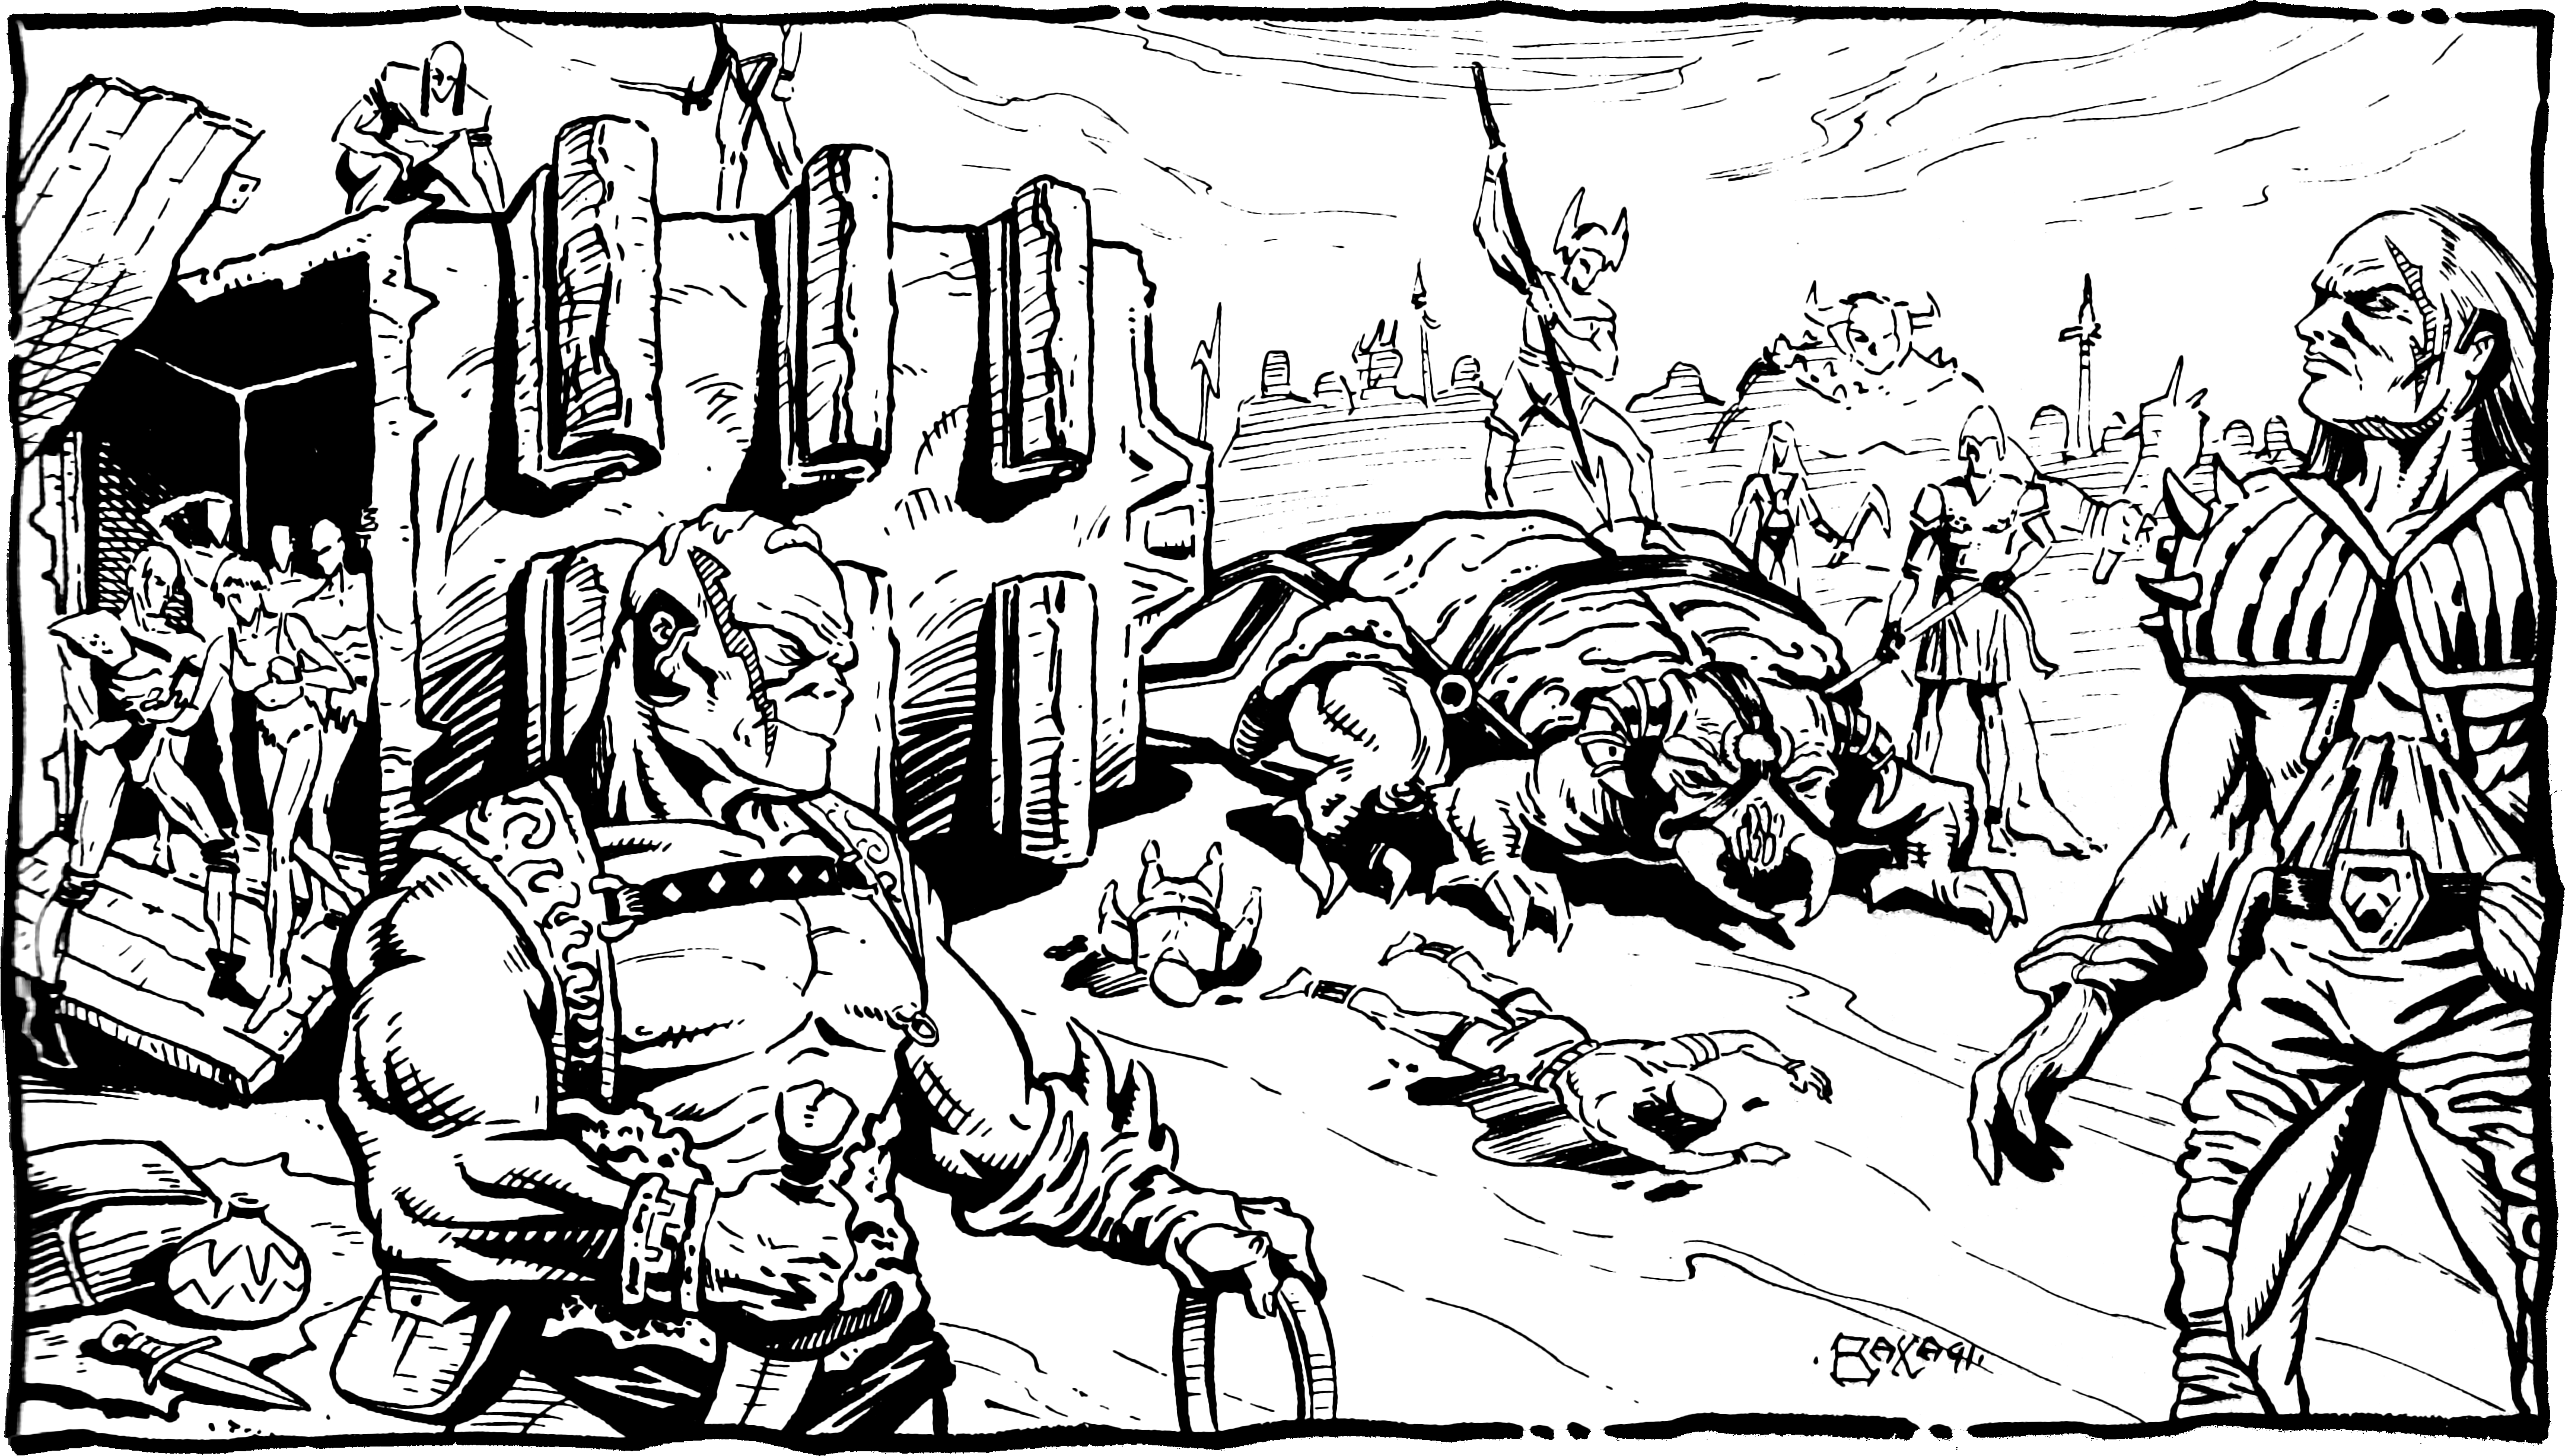
\includegraphics[width=\textwidth]{images/raiders-2.png}
\WOTC
\end{figure*}

\Capitalize{D}{ark} Sun 3.5 is a new edition of the {\tableheader Dark Sun} campaign setting, written as a revision of athas.org's {\tableheader Dark Sun} 3 rulebook and the \emph{Athasian Emporium}. This rulebook condenses all d20 System information available under OGL, including psionic rules, but it also changes the system a bit. In addition, you might find useful to download the \emph{Terrors of Athas} (ToA), \emph{Terrors of the Dead Lands} (TotDL), and \emph{Faces of the Forgotten North} (FFN), since this book does not contain information on monsters.

This document is intended for an audience already familiar with the {\tableheader Dark Sun} campaign setting, and does not attempt to detail the world of Athas in full. For more information on Athas, visit \url{www.athas.org}---the official {\tableheader Dark Sun} website. In addition to the latest version of this document, you may find other {\tableheader Dark Sun} material available as free downloads.

All {\tableheader Dark Sun} products published by TSR may be purchased from RPGNow! as PDF downloads.

\section{This is Athas}
Athas' savage, primal landscape is the result of long centuries of ecological and magical abuses. The world is dying. It breathes its last gasps as water turns to silt, grasslands become sandy wastes, and jungles decay into stony barrens. Still, life finds ways to endure even in these hellish conditions. In fact, it thrives.

Children growing up beneath the crimson sun don't aspire to become heroes. True heroes who champion causes or seek to make the world a better place are as rare as steel on Athas. Living to see the next dawn is more important than defending a set of beliefs, so survival ultimately motivates all living creatures---not virtue or righteousness.

But heroes are desperately needed in this harsh, savage world... Heroes like the ones who stepped forward to destroy the sorcerer-king Kalak and set Tyr free. Heroes like those who risked everything to kill the Dragon and keep Rajaat the Warbringer from devastating the land.

Today, Athas rushes toward its future. If the course of destruction is to be diverted, of Athas is to be restored, then more heroes must grab the reins of destiny and give new hope and promise to the world.

\subsection{Ten Things You Need to Know}
Every Dungeon Master and player needs to know and remember these facts about the world of Athas.

\begin{enumerate}
\item \textbf{Dark Sun is Different from Traditional D\&D.} Many monsters, prestige classes, spells or magic items from the core rulebooks simply are not available in Athas. Many races were extinguished from Athas during the Cleansing Wars. This is because Athas has a very different background than most D\&D settings. Check with your DM to see which options you have to choose from before building your character.

\item \textbf{Tone and Attitude.} Athas puts the survival of the fittest concept to its fullest. Those who cannot adapt to endure the tyrannical sorcerer-kings, the unrelenting sun, or the many dangers of the wastes will certainly perish. Illiteracy and slavery are commonplace, while magic is feared and hated. The term ``hero'' has a very different meaning on Athas.

\item \textbf{A Burnt World.} Thousands of years of reckless spellcasting and epic wars have turned Athas into a barren world, on the verge of an ecological collapse. From the first moments of dawn until the last twinkling of dusk, the crimson sun shimmers in the olive-tinged sky like a fiery puddle of blood, creating temperatures up to 65$^\circ$ C (150$^\circ$ F) by late afternoon. Waters is scarce, so most Athasians need to come up with alternative solutions for dealing with the heat or perish.

\item \textbf{A World Without Metal.} Metals are very rare on Athas. Its scarcity has forced Athasians to rely on barter and different materials, such as ceramic, to use as currency. It also hampers industrial and economic development as well; mills and workshops rarely have quality tools to produce everyday products. Even though most Athasians have developed ways of creating weapons and armor made of nonmetallic components, but the advantage of having metal equipment in battle is huge.

\item \textbf{The Will and The Way.} From the lowliest slave to the most powerful sorcerer-king, psionics pervade all levels of Athasian society. Virtually every individual has some mental ability, and every city-state has some sort of psionic academy available. Athasians use the term Will to refer to someone's innate ability for psionics and the Way for the study of psionics.

\item \textbf{A World Without Gods.} Athas is a world without true deities. Powerful sorcerer-kings often masquerade as gods but, though their powers are great and their worshipers many, they are not true gods. Arcane magic require life force, either from plants or animals, to be used. All divine power comes from the Elemental planes and the spirits of the land that inhabit geographic features.

\item \textbf{Planar Insulation.} Barriers exist between Athas and other planes. In the case of other planes of existence, the Gray impedes planar travel, except to the Elemental Planes. Consequently, travel via spelljamming is impossible, and planar travel is much more difficult. The same holds true for those trying to contact or reach Athas. The barrier formed by the Gray impedes travel in both directions.

\item \textbf{The Struggle For Survival.} The basic necessities of life are scarce on Athas. This means that every society must devote itself to attaining food and safeguarding its water supply, while protecting themselves from raiding tribes, Tyr-storms, and other city-states. This essentially means that most Athasian must devout a large deal of their lives just to survive.

\item \textbf{The Seven City-states.} The Tyr Region is the center of the world of Athas, at least as far as the people of the seven city-states are concerned. It's here, along the shores of the Silt Sea and in the shadows of the Ringing Mountains that civilization clings to a few scattered areas of fertile land and fresh water. The majority of the population lives in the city-states of Tyr, Urik, Raam, Draj, Nibenay, Gulg, and Balic. The remainder lives in remote villages built around oases and wells, or wanders about in nomadic tribes searching for what they need to survive.

\item \textbf{New and Changed Races.} The common races found in D\&D changed with the harsh planet, elves are tireless nomads, dwarves are bald and have a focused mind, half-elves struggle to fit in the society, and halflings are cannibals living in the jungles. In addition to those races, players can choose to play aarakocra, half-giants, muls, pterrans, and thri-kreen. Aarakocra are avian freedom-loving creatures, but extremely zealous and xenophobic. Half-giants are creatures with great strength, but dull wits. Muls are a hybrid race that combines the natural dwarven resilience and stubbornness with the adaptability from humans. Pterrans are reptilian nature-worshiping creatures that are always in the pursuit of their ``life paths''. Thri-kreen are insectoid creatures that roam the Athasian wastes in search for prey.
\end{enumerate}

\subsection{The Five Ages of Play}
{\tableheader Dark Sun} 3.5 supports adventures and campaigns set in many different ages, five of which are detailed in this book. You can set your campaign right after the events of the Prism Pentad. Known as the Age of Heroes, this is a period that fundamentally changed the world, when individuals begun fighting back all the tyranny and oppression, ending up with several sorcerer-kings dead and the first free city of the Tablelands appeared.

Or, you can go backward in time to the classic period where most sorcerer-kings were still alive and play during the Brown Age or the Age of Sorcerer-kings, when the world was becoming more and more a wasteland by defiling magic, and the Dragon of Tyr was almighty.

Or, you can go even more backward in time and play during the Cleansing Wars, when Rajaat unleashed his human armies and his Champions in order to wipe out all other intelligent races from the face of Athas.

Or, you can go to Green Age, when the New Races began populating the lands left unscathed by the receding waves, and the first great cities were found, and psionics started to show its true power.

Or, you can go to the very first age, known as the Blue Age, when the world was still young and the only intelligent races where the rhulisti, the ancient halflings, and the kreen, lived in a world filled with oceans and a blue sun, and magic was nonexistent.

In addition, the rules set in this book can be used to support campaigns set in other ages. For example, you could forward to several hundred years into the future, in a world that could be either devastated by the Kreen invasion, or that has just begun to heal from most of the damage it suffered since Rajaat discovered arcane magic. Although these ages are not covered in this book, the rules herein can be used as a basis for play in them.

\section{Where to Begin}
Players should begin by creating their {\tableheader Dark Sun} character after reading the first seven chapters of this book. Players may also want to read the timeline in order to understand the history of Athas. Remember to discuss with your DM before creating your character to find out what options and other books are allowed in his campaign.

The DM should start with \chapref{Life on Athas} and read material relevant to the locations, \chapref{Athasian Campaigns} for guidelines and tips when running your campaign, and \chapref{Others Eras of Play} to understand more about the era of play on which your campaign will focus.

\subsection{What You Need to Play}
This book contains revisions on the material from the three core rulebooks for {\tableheader Dungeons \& Dragons 3.5} and the \emph{Expanded Psionics Handbook} released under Open Game License (OGL). Throughout this book, superscript abbreviations are often used to denote game elements that appear in certain supplements: \emph{Complete Adventurer} (CAd), \emph{Complete Arcane} (CAr), \emph{Complete Champion} (CC), \emph{Complete Divine} (CD), \emph{Complete Mage} (CM), \emph{Complete Psionics} (CP), \emph{Complete Scoundrel} (CS), \emph{Complete Warrior} (CW), \emph{Player's Handbook II} (PH2). Having any of all of these supplements will enhance your enjoyment of this book, but they are not required.

\subsection{What Changed?}
Many new options were added to previous base classes, and some have been completely rewritten. Getting inspiration on the 5th edition, advantage and disadvantage were added to the system as well as multiclass prerequisites for base classes. Spell lists, domains, and magical items were changed. For a summary of all the changes between the d20 System rules under OGL and this book, see \apxref{Changes from d20 System}.

There are changes between the original \url{www.athas.org} rulebook and this revision, with some prestige classes being excluded, and others being reworked. New feats were also added and some of the previous ones were reworked. For a summary of all the changes between the \url{www.athas.org} rulebook and this book, see \apxref{Changes from Dark Sun 3}.

% \begin{figure}[t!]
% \centering
% 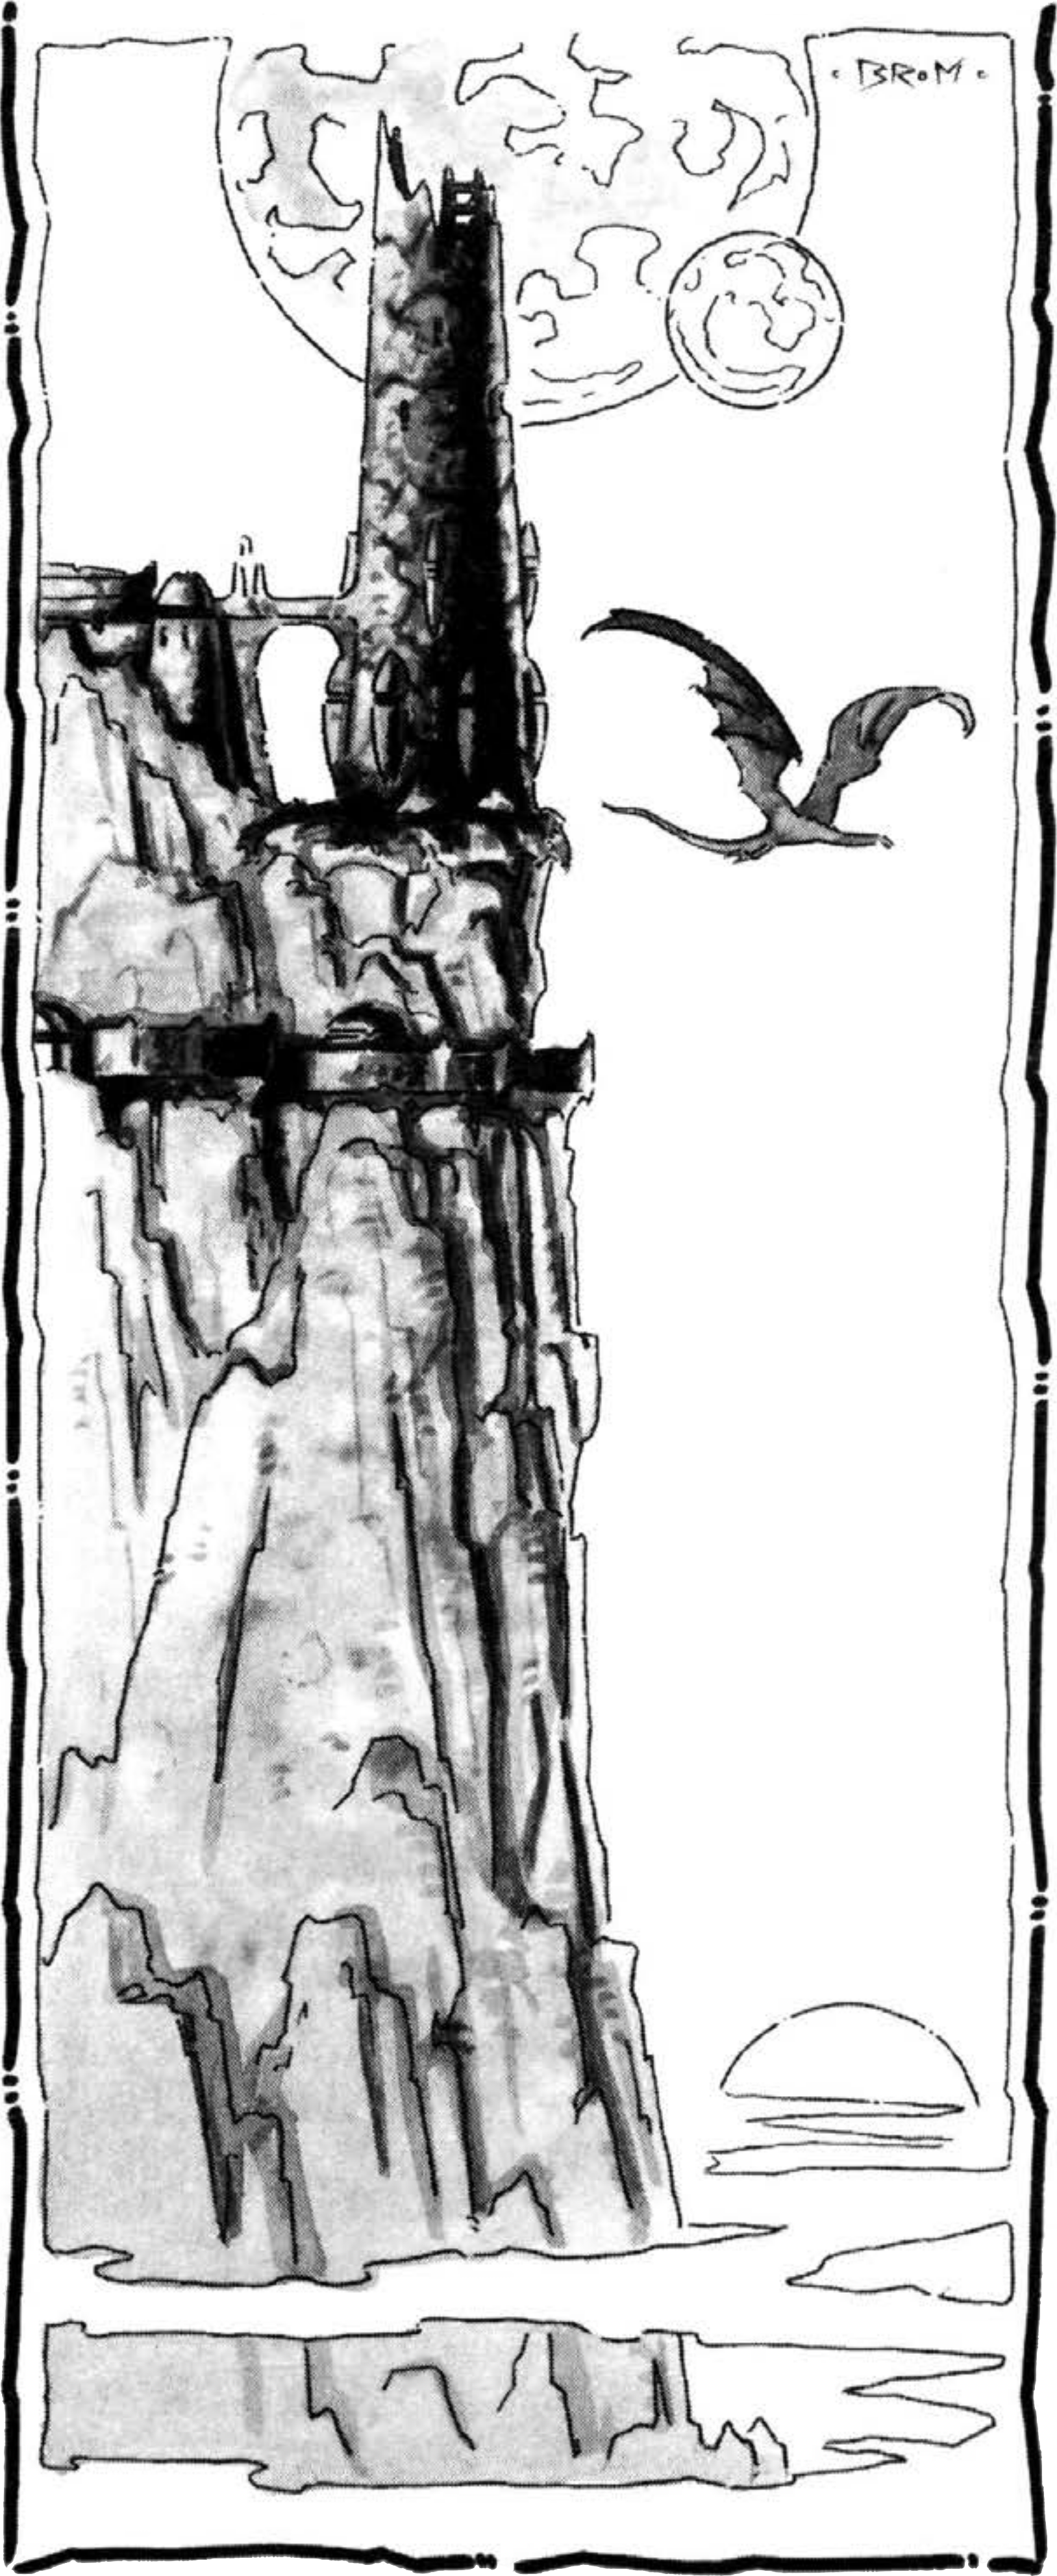
\includegraphics[width=\columnwidth-4mm]{images/tower-1.png}
% \WOTC
% \end{figure}

\clearpage
\section{The Core Mechanic}
Whenever you attempt an action that has some chance of failure, you roll a twenty-sided die (d20). To determine if your character succeeds at a task you do this:

\begin{itemize*}
\item Roll a d20.
\item Add any relevant modifiers.
\item Compare the result to a target number.
\item If the result equals or exceeds the target number, your character succeeds. If the result is lower than the target number, you fail.
\end{itemize*}

\subsection{Dice}
Dice rolls are described with expressions such as ``3d4+3,'' which means ``roll three four-sided dice and add 3'' (resulting in a number between 6 and 15). The first number tells you how many dice to roll (adding the results together). The number immediately after the ``d'' tells you the type of die to use. Any number after that indicates a quantity that is added or subtracted from the result.

\textbf{d\%:} Percentile dice work a little differently. You generate a number between 1 and 100 by rolling two different ten-sided dice. One (designated before you roll) is the tens digit. The other is the ones digit. Two 0s represent 100.

\subsection{Modifiers}
A modifier is any bonus or penalty applying to a die roll. A positive modifier is a bonus, and a negative modifier is a penalty.

\subsubsection{Stacking}
In most cases, modifiers to a given check or roll stack (combine for a cumulative effect) if they come from different sources and have different types (or no type at all), but do not stack if they have the same type or come from the same source (such as the same spell cast twice in succession). If the modifiers to a particular roll do not stack, only the best bonus and worst penalty applies. Dodge bonuses and circumstance bonuses however, do stack with one another unless otherwise specified.

\subsubsection{Modifier Types}
\textbf{Ability Modifier:} The bonus or penalty associated with a particular ability score. Ability modifiers apply to die rolls for character actions involving the corresponding abilities.

\textbf{Alchemical Bonus:} An alchemical bonus is granted by the use of a nonmagical, alchemical substance such as antitoxin.

\textbf{Armor Bonus:} An armor bonus applies to Armor Class and is granted by armor or by a spell or magical effect that mimics armor. Armor bonuses stack with all other bonuses to Armor Class (even with natural armor bonuses) except other armor bonuses. An armor bonus doesn't apply against touch attacks, except for armor bonuses granted by force effects (such as the mage armor spell) which apply against incorporeal touch attacks, such as that of a shadow.

\textbf{Circumstance Modifier:} A circumstance bonus (or penalty) arises from specific conditional factors impacting the success of the task at hand. Circumstance bonuses stack with all other bonuses, including other circumstance bonuses, unless they arise from essentially the same source.

\textbf{Competence Modifier:} A competence bonus (or penalty) affects a character's performance of a particular task, as in the case of the bardic ability to inspire competence. Such a bonus may apply on attack rolls, saving throws, skill checks, caster level checks, or any other checks to which a bonus relating to level or skill ranks would normally apply. It does not apply on ability checks, damage rolls, initiative checks, or other rolls that aren't related to a character's level or skill ranks. Multiple competence bonuses don't stack; only the highest bonus applies.

\textbf{Deflection Bonus:} A deflection bonus affects Armor Class and is granted by a spell or magic effect that makes attacks veer off harmlessly. Deflection bonuses stack with all other bonuses to AC except other deflection bonuses. A deflection bonus applies against touch attacks.

\textbf{Dodge Bonus:} A dodge bonus improves Armor Class (and sometimes Reflex saves) resulting from physical skill at avoiding blows and other ill effects. Dodge bonuses are never granted by spells or magic items. Any situation or effect (except wearing armor) that negates a character's Dexterity bonus also negates any dodge bonuses the character may have. Dodge bonuses stack with all other bonuses to AC, even other dodge bonuses. Dodge bonuses apply against touch attacks.

\textbf{Enhancement Bonus:} An enhancement bonus represents an increase in the sturdiness and/or effectiveness of armor or natural armor, or the effectiveness of a weapon, or a general bonus to an ability score. Multiple enhancement bonuses on the same object (in the case of armor and weapons), creature (in the case of natural armor), or ability score do not stack. Only the highest enhancement bonus applies. Since enhancement bonuses to armor or natural armor effectively increase the armor or natural armor's bonus to AC, they don't apply against touch attacks.

\textbf{Insight Bonus:} An insight bonus improves performance of a given activity by granting the character an almost precognitive knowledge of what might occur. Multiple insight bonuses on the same character or object do not stack. Only the highest insight bonus applies.

\textbf{Luck Modifier:} A luck modifier represents good (or bad) fortune. Multiple luck bonuses on the same character or object do not stack. Only the highest luck bonus applies.

\textbf{Morale Modifier:} A morale bonus represents the effects of greater hope, courage, and determination (or hopelessness, cowardice, and despair in the case of a morale penalty). Multiple morale bonuses on the same character do not stack. Only the highest morale bonus applies. Nonintelligent creatures (creatures with an Intelligence of 0 or no Intelligence at all) cannot benefit from morale bonuses.

\textbf{Natural Armor Bonus:} A natural armor bonus improves Armor Class resulting from a creature's naturally tough hide. Natural armor bonuses stack with all other bonuses to Armor Class (even with armor bonuses) except other natural armor bonuses. Some magical effects (such as the barkskin spell) grant an enhancement bonus to the creature's existing natural armor bonus, which has the effect of increasing the natural armor's overall bonus to Armor Class. A natural armor bonus doesn't apply against touch attacks.

\textbf{Profane Modifier:} A profane bonus (or penalty) stems from the power of evil. Multiple profane bonuses on the same character or object do not stack. Only the highest profane bonus applies.

\textbf{Racial bonus:} A bonus granted because of the culture a particular creature was brought up in or because of innate characteristics of that type of creature. If a creature's race changes (for instance, if it dies and is reincarnated), it loses all racial bonuses it had in its previous form.

\textbf{Resistance Bonus:} A resistance bonus affects saving throws, providing extra protection against harm. Multiple resistance bonuses on the same character or object do not stack. Only the highest resistance bonus applies.

\textbf{Sacred Modifier:} A sacred bonus (or penalty) stems from the power of good. Multiple sacred bonuses on the same character or object do not stack. Only the highest sacred bonus applies.

\textbf{Shield Bonus:} A shield bonus improves Armor Class and is granted by a shield or by a spell or magic effect that mimics a shield. Shield bonuses stack with all other bonuses to AC except other shield bonuses. A magic shield typically grants an enhancement bonus to the shield's shield bonus, which has the effect of increasing the shield's overall bonus to AC. A shield bonus granted by a spell or magic item typically takes the form of an invisible, tangible field of force that protects the recipient. A shield bonus doesn't apply against touch attacks.

\textbf{Size Modifier:} A size bonus or penalty is derived from a creature's size category. Size modifiers of different kinds apply to Armor Class, attack rolls, Hide checks, grapple checks, and various other checks.

\subsubsection{Rounding Fractions}
In general, if you wind up with a fraction, round down, even if the fraction is one-half or larger.

\textit{Exception:} Certain rolls, such as damage and hit points, have a minimum of 1.

% \begin{figure*}[b!]
% \centering
% 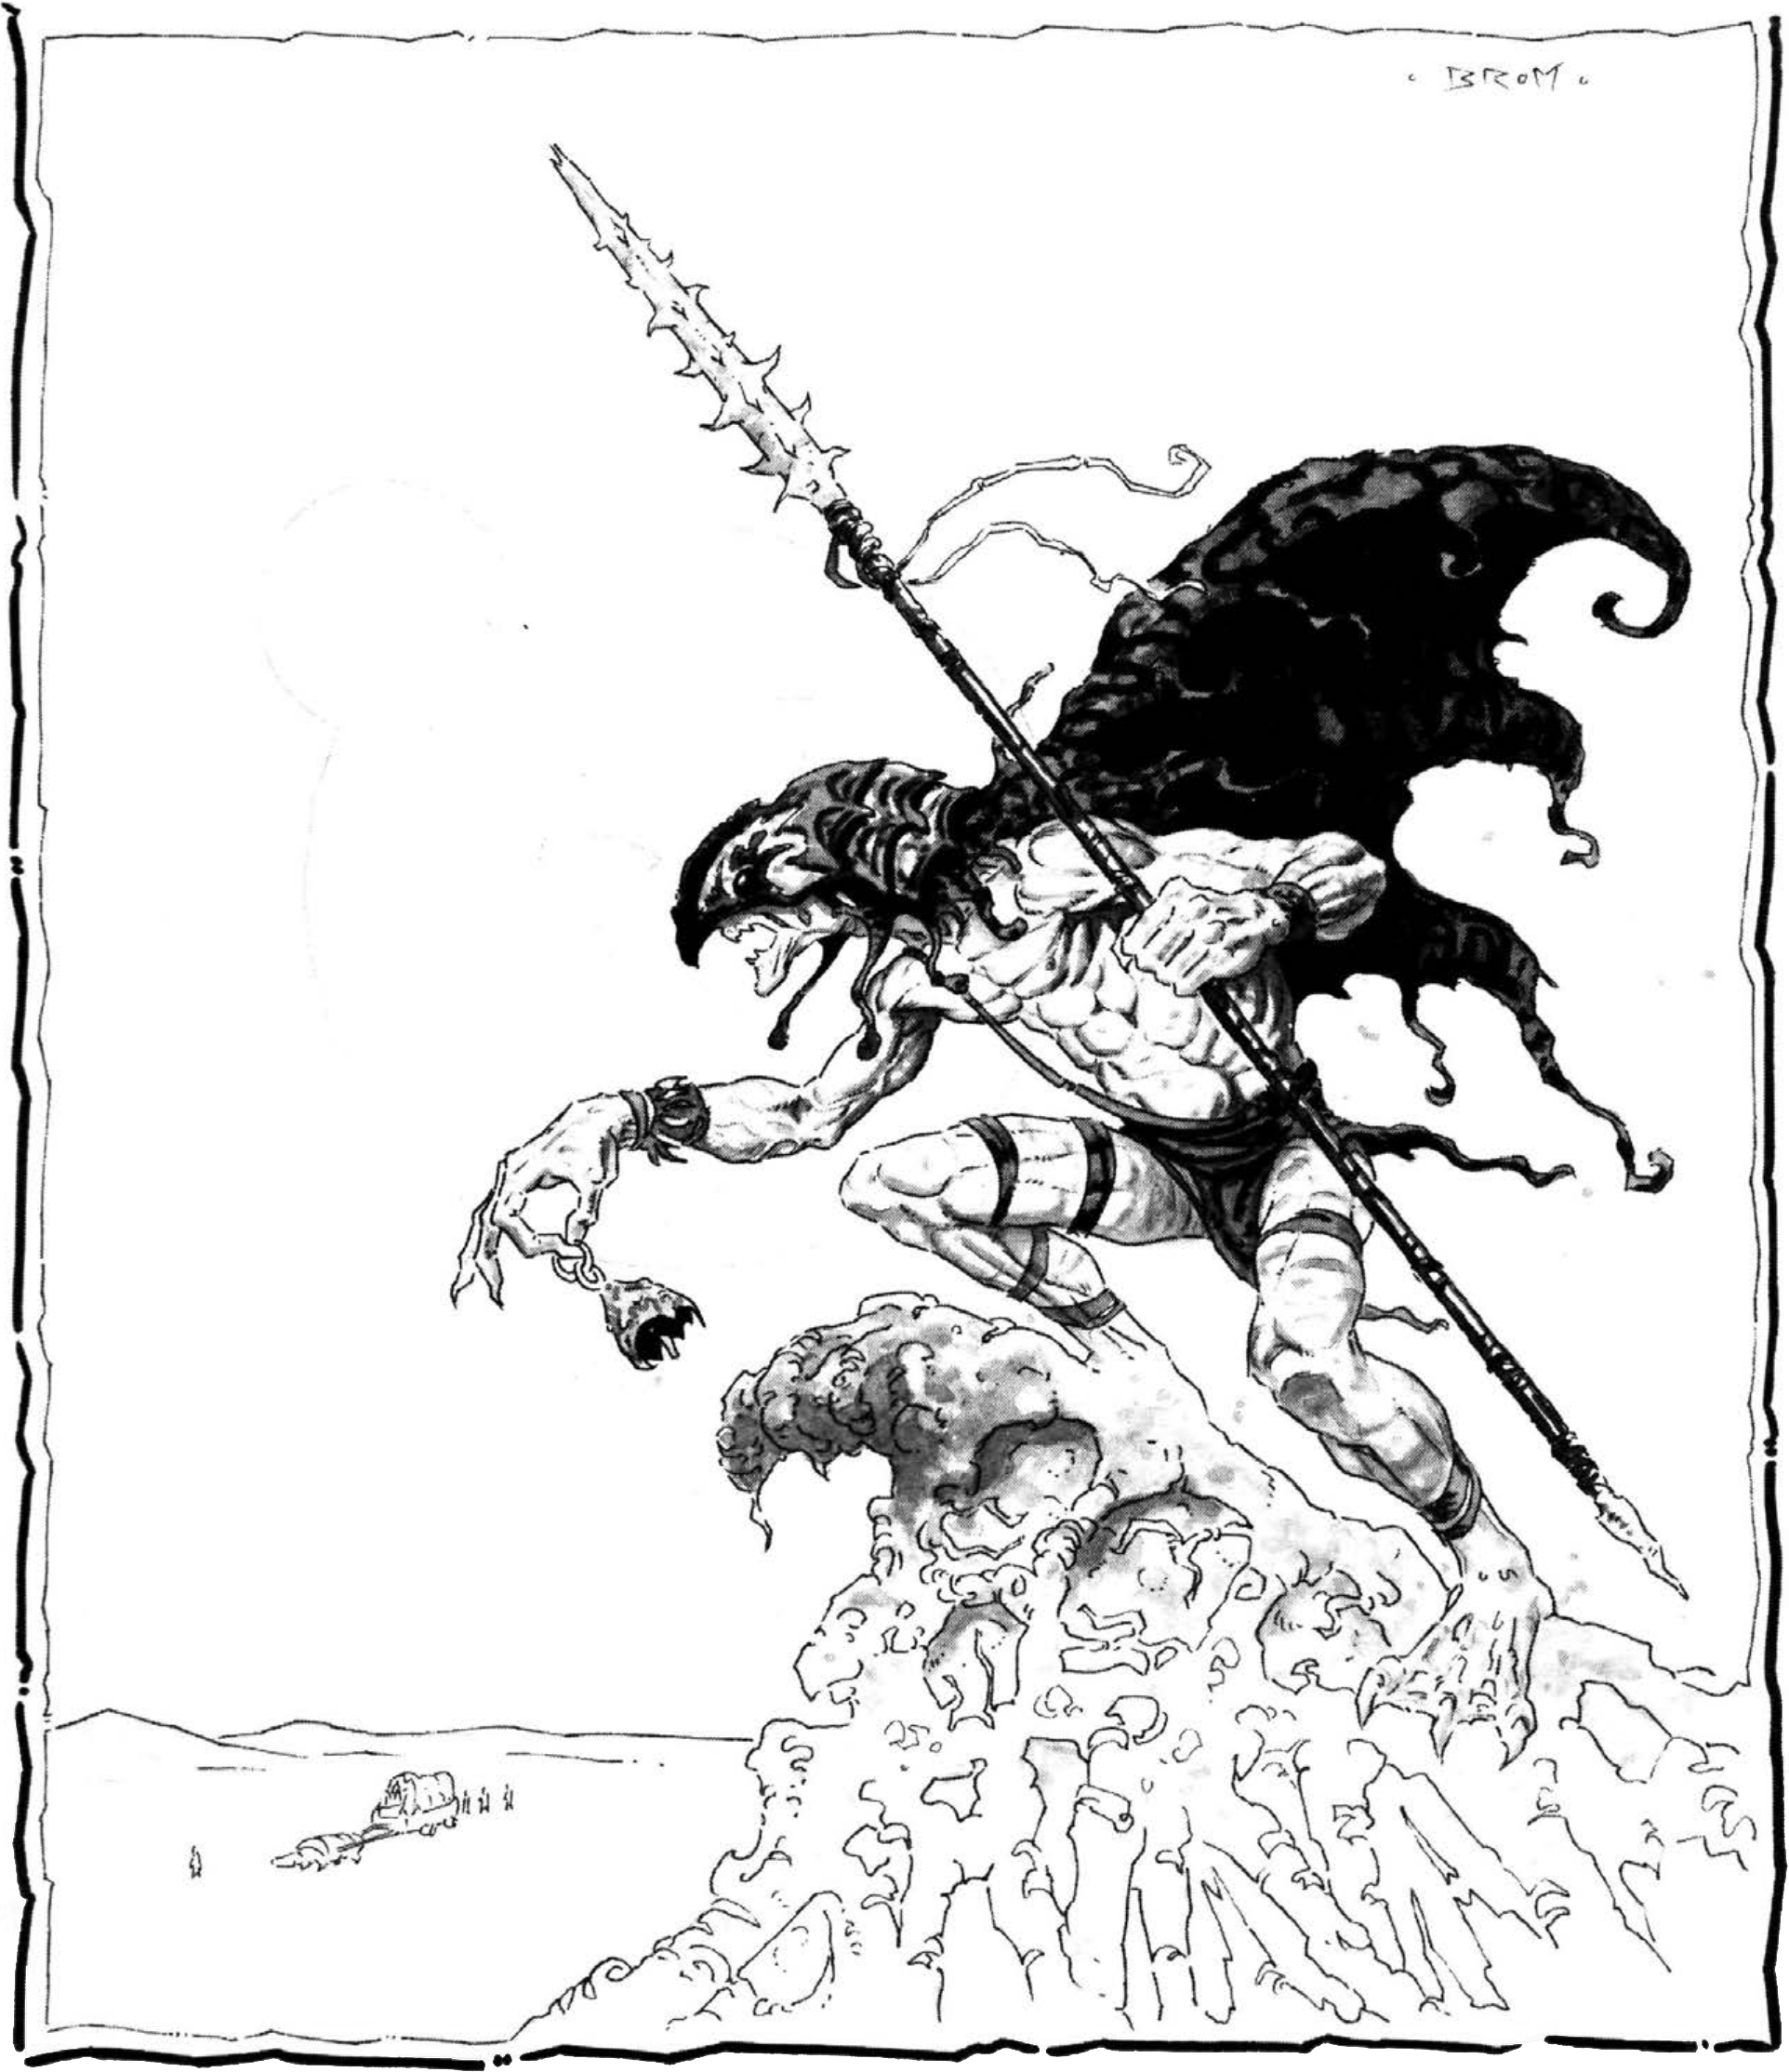
\includegraphics[width=\textwidth]{images/wizard-3.png}
% \WOTC
% \end{figure*}

\subsection{Multiplying}
Sometimes a rule makes you multiply a number or a die roll. As long as you're applying a single multiplier, multiply the number normally. When two or more multipliers apply to any abstract value (such as a modifier or a die roll), however, combine them into a single multiple, with each extra multiple adding 1 less than its value to the first multiple. Thus, a double ($\times$2) and a double ($\times$2) applied to the same number results in a triple ($\times$3, because 2 + 1 = 3).

When applying multipliers to real-world values (such as weight or distance), normal rules of math apply instead. A creature whose size doubles (thus multiplying its weight by 8) and then is turned to stone (which would multiply its weight by a factor of roughly 3) now weighs about 24 times normal, not 10 times normal. Similarly, a blinded creature attempting to negotiate difficult terrain would count each square as 4 squares (doubling the cost twice, for a total multiplier of $\times$4), rather than as 3 squares (adding 100\% twice).

\subsection{Advantage and Disadvantage}
Sometimes a special ability or spell tells you that you have advantage or disadvantage on an ability check, a saving throw, or an attack roll. When that happens, you roll a second d20 when you make the roll. Use the higher of the two rolls if you have advantage, and use the lower roll if you have disadvantage. For example, if you have disadvantage and roll a 17 and a 5, you use the 5. If you instead have advantage and roll those numbers, you use the 17.

If multiple situations affect a roll and each one grants advantage or imposes disadvantage on it, you don't roll more than one additional d20. If two favorable situations grant advantage, for example, you still roll only one additional d20.

If circumstances cause a roll to have both advantage and disadvantage, you are considered to have neither of them, and you roll one d20. This is true even if multiple circumstances impose disadvantage and only one grants advantage or vice versa. In such a situation, you have neither advantage nor disadvantage.
\Chapter{Abilities}
{Life is a mysterious and resilient thing. Even in the starkest wastes of Athas, the careful observer finds it clinging to the horns of sand dunes, peeking out from beneath wind-raked boulders, and creeping along the cracked plains of sun-baked clay.
To survive, almost every form of life has become a monster. On the increasingly infertile world of Athas, these adaptations have taken an almost diabolical turn. The land is so barren that every form of life, to one extent or another, is both predator and prey.}
{The Wanderer's Journal}

\Capitalize{E}{ach} character in {\tableheader Dark Sun} has six abilities: Strength (abbreviated Str), Dexterity (Dex), Constitution (Con), Intelligence (Int), Wisdom (Wis), and Charisma (Cha). Each of your abilities above average gives you a bonus on certain die rolls, and abilities below average give you a penalty on other die rolls.

\section{Ability Scores}
Previous editions used a rolling method that produced, on average, higher stats. This was supposed to convey that Athas was a much harsher world than normal D\&D campaign worlds, and that its denizens had adapted to compensate. However, the meaning of an attribute has changed in 3rd edition, and attributes start having a positive effect much sooner than they did in 2nd edition. Whereas many stats didn't start having a positive effect until they were at least 14, now as low as 12 have a positive effect. Using higher overall attributes for characters in {\tableheader Dark Sun} actually makes it easier for characters to survive and overcome obstacles that should be challenging, which would mean that the effective difficulty of a campaign would actually be lower using this stat generation method.

% \subsection{Creating Ability Scores}
% There are two methods for creating ability scores for your character: randomly or via point buy.  The average ability score for the typical commoner is 10 or 11, but your character is not typical. The most common ability scores for player characters (PCs) are 12 and 13.

% \subsubsection{Random Generation}
% To create an ability score for your character, roll 4d6. Disregard the lowest die roll and sum the rest. The result is a number between 3 (horrible) and 18 (tremendous)
% .
% Make this roll six times, recording each result on a piece of paper. Once you have six scores, assign each score to one of the six abilities.

% \subsubsection{Point Buy}
% All abilities scores start at 8. Take a number of points according to the type of your campaign to spread out among all abilities. For ability scores of 14 or lower, you buy additional points on a 1-for-1 basis. For ability scores higher than 14, it costs a little more.

% \Table{}{C C C C}{\tableheader Ability Score & \tableheader Point Cost & \tableheader Ability Score & \tableheader Point Cost \\
%   9 & 1 & 14 & 6 \\
%   10 & 2 & 15 & 8 \\
%   11 & 3 & 16 & 10 \\
%   12 & 4 & 17 & 13 \\
%   13 & 5 & 18 & 16}

% \Table{}{X r}{\tableheader Type of Campaign & \tableheader Points Allowed\\
%   Low-powered campaign & 15 points \\
%   Challenging campaign & 22 points \\
%   Normal campaign & 25 points \\
%   Tougher campaign & 28 points \\
%   High-powered campaign & 32 points}

\subsection{Ability Modifiers}

Each ability, after changes made because of race, has a modifier ranging from $-5$ to +5. \tabref{Ability Modifiers and Bonus Spells} shows the modifier for each score. It also shows bonus spells, which you'll need to know about if your character is a spellcaster.

The modifier is the number you apply to the die roll when your character tries to do something related to that ability. You also use the modifier with some numbers that aren't die rolls. A positive modifier is called a bonus, and a negative modifier is called a penalty.

\BigTable{Ability Modifiers and Bonus Spells}{X c *{10}{C}}{
  \hline
  \rowcolor{white}
  & & \multicolumn{10}{c}{\tableheader Bonus Spells (by spell level)} \\
  \hline
  \rowcolor{white}
  \tableheader Score & \tableheader Modifier & \tableheader 0 & \tableheader 1st & \tableheader 2nd & \tableheader 3rd & \tableheader 4th & \tableheader 5th & \tableheader 6th & \tableheader 7th & \tableheader 8th & \tableheader 9th \\
  1 & $-5$ & \cellcolor{TableColor}&\cellcolor{TableColor}&\cellcolor{TableColor}&\cellcolor{TableColor}&\cellcolor{TableColor}&\cellcolor{TableColor}&\cellcolor{TableColor}&\cellcolor{TableColor}&\cellcolor{TableColor}&\cellcolor{TableColor}\\
  2-3 & $-4$ & \cellcolor{TableColor}&\cellcolor{TableColor}&\cellcolor{TableColor}&\cellcolor{TableColor}&\cellcolor{TableColor}&\cellcolor{TableColor}&\cellcolor{TableColor}&\cellcolor{TableColor}&\cellcolor{TableColor}&\cellcolor{TableColor}\\
  4-5 & $-3$ & \cellcolor{TableColor}&\cellcolor{TableColor}&\cellcolor{TableColor}&\cellcolor{TableColor}&\cellcolor{TableColor}&\cellcolor{TableColor}&\cellcolor{TableColor}&\cellcolor{TableColor}&\cellcolor{TableColor}&\cellcolor{TableColor}\\
  6-7 & $-2$ & \cellcolor{TableColor}&\cellcolor{TableColor}&\cellcolor{TableColor}&\cellcolor{TableColor}&\cellcolor{TableColor}&\cellcolor{TableColor}&\cellcolor{TableColor}&\cellcolor{TableColor}&\cellcolor{TableColor}&\cellcolor{TableColor}\\
  8-9 & $-1$ &\multicolumn{10}{c}{\multirow{-5}{*}{\bfseries Can't cast spells tied to this ability}}\\
  10--11 & 0 &&&&&&&&&&\\
  12--13 & +1 && 1 &&&&&&&&\\
  14--15 & +2 && 1 & 1 &&&&&&&\\
  16--17 & +3 && 1 & 1 & 1 &&&&&&\\
  18--19 & +4 && 1 & 1 & 1 & 1 &&&&&\\
  20--21 & +5 && 2 & 1 & 1 & 1 & 1 &&&&\\
  22--23 & +6 && 2 & 2 & 1 & 1 & 1 & 1 &&&\\
  24--25 & +7 && 2 & 2 & 2 & 1 & 1 & 1 & 1 &&\\
  26--27 & +8 && 2 & 2 & 2 & 2 & 1 & 1 & 1 & 1 &\\
  28--29 & +9 && 3 & 2 & 2 & 2 & 2 & 1 & 1 & 1 & 1 \\
  30--31 & +10 && 3 & 3 & 2 & 2 & 2 & 2 & 1 & 1 & 1 \\
  32--33 & +11 && 3 & 3 & 3 & 2 & 2 & 2 & 2 & 1 & 1 \\
  34--35 & +12 && 3 & 3 & 3 & 3 & 2 & 2 & 2 & 2 & 1 \\
  36--37 & +13 && 4 & 3 & 3 & 3 & 3 & 2 & 2 & 2 & 2 \\
  38--39 & +14 && 4 & 4 & 3 & 3 & 3 & 3 & 2 & 2 & 2 \\
  40--41 & +15 && 4 & 4 & 4 & 3 & 3 & 3 & 3 & 2 & 2
}

\BigTable{Ability Scores and Bonus Power Points}{l *{20}{C}}{
  \hline
  \rowcolor{white}
  & \multicolumn{20}{c}{\tableheader Bonus Power Points (by class level)} \\
  \hline
  \rowcolor{white}
\tableheader Score & \tableheader 1st & \tableheader 2nd & \tableheader 3rd & \tableheader 4th & \tableheader 5th & \tableheader 6th & \tableheader 7th & \tableheader 8th & \tableheader 9th & \tableheader 10th & \tableheader 11th & \tableheader 12th & \tableheader 13th & \tableheader 14th & \tableheader 15th & \tableheader 16th & \tableheader 17th & \tableheader 18th & \tableheader 19th & \tableheader 20th \\
10--11 &&&&&&&&&&&&&&&&&&&&\\
12--13 && 1 & 1 & 2 & 2 & 3 & 3 & 4 & 4 & 5 & 5 & 6 & 6 & 7 & 7 & 8 & 8 & 9 & 9 & 10 \\
14--15 & 1 & 2 & 3 & 4 & 5 & 6 & 7 & 8 & 9 & 10 & 11 & 12 & 13 & 14 & 15 & 16 & 17 & 18 & 19 & 20 \\
16--17 & 1 & 3 & 4 & 6 & 7 & 9 & 10 & 12 & 13 & 15 & 16 & 18 & 19 & 21 & 22 & 24 & 25 & 27 & 28 & 30 \\
18--19 & 2 & 4 & 6 & 8 & 10 & 12 & 14 & 16 & 18 & 20 & 22 & 24 & 26 & 28 & 30 & 32 & 34 & 36 & 38 & 40 \\
20--21 & 2 & 5 & 7 & 10 & 12 & 15 & 17 & 20 & 22 & 25 & 27 & 30 & 32 & 35 & 37 & 40 & 42 & 45 & 47 & 50 \\
22--23 & 3 & 6 & 9 & 12 & 15 & 18 & 21 & 24 & 27 & 30 & 33 & 36 & 39 & 42 & 45 & 48 & 51 & 54 & 57 & 60 \\
24--25 & 3 & 7 & 10 & 14 & 17 & 21 & 24 & 28 & 31 & 35 & 38 & 42 & 45 & 49 & 52 & 56 & 59 & 63 & 66 & 70 \\
26--27 & 4 & 8 & 12 & 16 & 20 & 24 & 28 & 32 & 36 & 40 & 44 & 48 & 52 & 56 & 60 & 64 & 68 & 72 & 76 & 80 \\
28--29 & 4 & 9 & 13 & 18 & 22 & 27 & 31 & 36 & 40 & 45 & 49 & 54 & 58 & 63 & 67 & 72 & 76 & 81 & 85 & 90 \\
30--31 & 5 & 10 & 15 & 20 & 25 & 30 & 35 & 40 & 45 & 50 & 55 & 60 & 65 & 70 & 75 & 80 & 85 & 90 & 95 & 100 \\
32--33 & 5 & 11 & 16 & 22 & 27 & 33 & 38 & 44 & 49 & 55 & 60 & 66 & 71 & 77 & 82 & 88 & 93 & 99 & 104 & 110 \\
34--35 & 6 & 12 & 18 & 24 & 30 & 36 & 42 & 48 & 54 & 60 & 66 & 72 & 78 & 84 & 90 & 96 & 102 & 108 & 114 & 120 \\
36--37 & 6 & 13 & 19 & 26 & 32 & 39 & 45 & 52 & 58 & 65 & 71 & 78 & 84 & 91 & 97 & 104 & 110 & 117 & 123 & 130 \\
38--39 & 7 & 14 & 21 & 28 & 35 & 42 & 49 & 56 & 63 & 70 & 77 & 84 & 91 & 98 & 105 & 112 & 119 & 126 & 133 & 140 \\
40--41 & 7 & 15 & 22 & 30 & 37 & 45 & 52 & 60 & 67 & 75 & 82 & 90 & 97 & 105 & 112 & 120 & 127 & 135 & 142 & 150}

\subsection{Abilities, Spellcasters and \hskip4em Manifesters}
The ability that governs bonus spells depends on what type of spellcaster your character is: Intelligence for wizards; Wisdom for clerics, druids, and rangers; or Charisma for templars. In addition to having a high ability score, a spellcaster must be of high enough class level to be able to cast spells of a given spell level.

Psions also depend on abilities for additional power for each discipline: Intelligence for metacreativity and psychokinesis, Wisdom for clairscience and telepathy, and Constitution for psychometabolism and psychoportation. The modifier for this ability is referred to as your key ability modifier. If your character's key ability score is 9 or lower, you can't manifest powers from that discipline.
% Psionic classes also depend on abilities for additional power: Intelligence for psions, Wisdom for psychic warriors, and Charisma for wilders. The modifier for this ability is referred to as your key ability modifier. If your character's key ability score is 9 or lower, you can't manifest powers from that psionic class.

Just as a high Intelligence score grants bonus spells to a wizard and a high Wisdom score grants bonus spells to a cleric, a character who manifests powers (psions) gains bonus power points according to his Intelligence score. Refer to \tabref{Ability Scores and Bonus Power Points}.

\subsubsection{How To Determine Bonus Power Points}
Your key ability score grants you additional power points equal to your key ability modifier $\times$ your manifester level $\times$ \onehalf. \tabref{Ability Scores and Bonus Power Points} shows these calculations for class levels 1st through 20th and key ability scores from 10 to 41.

\section{The Abilities}
Each ability partially describes your character and affects some of his or her actions.

\subsection{Strength (Str)}
Strength measures your character's muscle and physical power. This ability is especially important for gladiators, fighters, barbarians, and rangers because it helps them prevail in combat. Strength also limits the amount of equipment your character can carry.

You apply your character's Strength modifier to:
\begin{itemize*}
\item Melee attack rolls.
\item Damage rolls when using a melee weapon or a thrown weapon (including a sling). (Exceptions: Off-hand attacks receive only one-half the character's Strength bonus, while two-handed attacks receive one and a half times the Strength bonus. A Strength penalty, but not a bonus, applies to attacks made with a bow that is not a composite bow.)
\item \skill{Climb}, \skill{Jump}, and \skill{Swim} checks. These are the skills that have Strength as their key ability.
\item Strength checks (for breaking down doors and the like).
\end{itemize*}

\subsection{Dexterity (Dex)}
Dexterity measures hand-eye coordination, agility, reflexes, and balance. This ability is the most important one for rogues, and bards, but it's also high on the list for characters who typically wear light or medium armor (gladiators, rangers, wilders, and barbarians) or no armor at all (psions and wizards), and for anyone who wants to be a skilled archer.

You apply your character's Dexterity modifier to:
\begin{itemize*}
\item Ranged attack rolls, including those for attacks made with bows, crossbows, throwing axes, and other ranged weapons.
\item Armor Class (AC), provided that the character can react to the attack.
\item Reflex saving throws, for avoiding fireballs and other attacks that you can escape by moving quickly.
\item \skill{Balance}, \skill{Escape Artist}, \skill{Hide}, \skill{Move Silently}, \skill{Open Lock}, \skill{Ride}, \skill{Sleight of Hand}, \skill{Tumble}, and \skill{Use Rope} checks. These are the skills that have Dexterity as their key ability.
\end{itemize*}
\subsection{Constitution (Con)}
Constitution represents your character's health and stamina. A Constitution bonus increases a character's hit points, so the ability is important for all classes.

You apply your character's Constitution modifier to:
\begin{itemize*}
\item Each roll of a Hit Die (though a penalty can never drop a result below 1---that is, a character always gains at least 1 hit point each time he or she advances in level).
\item Fortitude saving throws, for resisting poison and similar threats.
\item \skill{Concentration} checks. Concentration is a skill, important to spellcasters, that has Constitution as its key ability.
\end{itemize*}

If a character's Constitution score changes enough to alter his or her Constitution modifier, the character's hit points also increase or decrease accordingly.

\subsection{Intelligence (Int)}
Intelligence determines how well your character learns and reasons. This ability is important for wizards because it affects how many spells they can cast, how hard their spells are to resist, and how powerful their spells can be. It's also important for any character who wants to have a wide assortment of skills.

You apply your character's Intelligence modifier to:
\begin{itemize*}
\item The number of languages your character knows at the start of the game.
\item The number of skill points gained each level. (But your character always gets at least 1 skill point per level.)
\item \skill{Appraise}, \skill{Craft}, \skill{Decipher Script}, \skill{Disable Device}, \skill{Forgery}, \skill{Knowledge}, \skill{Search}, and \skill{Spellcraft} checks. These are the skills that have Intelligence as their key ability.
\end{itemize*}

A wizard gains bonus spells based on her Intelligence score. The minimum Intelligence score needed to cast a wizard spell is 10 + the spell's level.

An animal has an Intelligence score of 1 or 2. A creature of human-like intelligence has a score of at least 3.

\subsection{Wisdom (Wis)}
Wisdom describes a character's willpower, common sense, perception, and intuition. While Intelligence represents one's ability to analyze information, Wisdom represents being in tune with and aware of one's surroundings. Wisdom is the most important ability for clerics and druids, and it is also important for rangers. If you want your character to have acute senses, put a high score in Wisdom. Every creature has a Wisdom score.

You apply your character's Wisdom modifier to:
\begin{itemize*}
\item Will saving throws (for negating the effect of charm person and other spells).
\item \skill{Heal}, \skill{Listen}, \skill{Profession}, \skill{Sense Motive}, \skill{Spot}, and \skill{Survival} checks. These are the skills that have Wisdom as their key ability.
\item Clerics, druids, and rangers get bonus spells based on their Wisdom scores. The minimum Wisdom score needed to cast a cleric, druid, or ranger spell is 10 + the spell's level.
\end{itemize*}

\subsection{Charisma (Cha)}
Charisma measures a character's force of personality, persuasiveness, personal magnetism, ability to lead, and physical attractiveness. This ability represents actual strength of personality, not merely how one is perceived by others in a social setting. Charisma is most important for templars. It is also important for clerics, since it affects their ability to turn undead. Every creature has a Charisma score.

You apply your character's Charisma modifier to:
\begin{itemize*}
\item \skill{Bluff}, \skill{Diplomacy}, \skill{Disguise}, \skill{Gather Information}, \skill{Handle Animal}, \skill{Intimidate}, \skill{Perform}, and \skill{Use Magic Device} checks. These are the skills that have Charisma as their key ability.
\item Checks that represent attempts to influence others.
\item Turning checks for clerics and templars attempting to turn zombies, vampires, and other undead.
\end{itemize*}

Templars get bonus spells based on their Charisma scores. The minimum Charisma score needed to cast a templar spell is 10 + the spell's level.

\subsection{Changing Ability Scores}
When an ability score changes, all attributes associated with that score change accordingly. A character does not retroactively get additional skill points for previous levels if she increases her intelligence.

\pagepdf*{images/color-halfelf-1.pdf}
\Chapter{Character Races}
{I live in a world of fire and sand. The crimson sun scorches the life from anything that crawls or flies, and storms of sand scour the foliage from the barren ground. Lightning strikes from the cloudless sky, and peals of thunder roll unexplained across the vast tablelands. Even the wind, dry and searing as a kiln, can kill a man with thirst.}
{The Wanderer's Journal}

\Capitalize{A}{thas} is a world of many races, from the gith who wander the deserts, to the tareks, too stubborn to know when they have died. Giants terrorize the Silt Sea, while belgoi steal grown men in the night. The magic of the Pristine Tower produces the New Races; most never see a second generation. Despite the variety of intelligent life, only a few races have the numbers to significantly impact the politics of the Tablelands.

Though the races of the {\tableheader Dark Sun} campaign setting resemble those of other campaign worlds, it is frequently in name only. The insular elves roam the Tablelands, trusted by no one but their own tribe-mates. Halflings are feral creatures, possessed of a taste for human flesh. Hairless dwarves work endlessly, their entire perception of the world filtered through the lens of a single, all-consuming task. Unsleeping thri-kreen roam the wastes, always hunting their next meal.

\section{Racial Characteristics}

\BigTablePair{Athasian Racial Ability Adjustments}{l l c L Y{22mm} l}{
\tableheader Race & \tableheader Type (Subtype) & \tableheader LA & \tableheader Ability Adjustments & \tableheader Favored Class & \tableheader Languages \\
Human      & Humanoid (human)    &    &                                                   & Any       & Common \\
Dwarf      & Humanoid (dwarf)    &    & +2 Strength, $-2$ Dexterity, +4 Constitution,
                                        \newline$-4$ Charisma                             & Gladiator & Common, Dwarven \\
Elf        & Humanoid (elf)      &    & +4 Dexterity, $-4$ Constitution, +2 Intelligence,
                                        \newline$-2$ Wisdom                               & Defiler, ranger, or templar & Common, Elven \\
Half-elf   & Humanoid (elf)      &    & +2 Dexterity, $-2$ Constitution                   & Any       & Common, Elven \\
Half-giant & Giant               & +2 & +8 Strength, +4 Constitution, $-4$ Intelligence,
                                        \newline$-4$ Wisdom, $-4$ Charisma                & Barbarian & Common \\
Halfling   & Humanoid (halfling) & +1 & $-4$ Strength, +4 Dexterity, +4 Wisdom,
                                        \newline$-2$ Charisma                             & Druid, ranger, or rogue & Halfling \\
Mul        & Humanoid (dwarf)    & +1 & +4 Strength, +2 Constitution, $-2$ Intelligence,
                                        \newline$-4$ Charisma                             & Fighter or gladiator & Common \\
Thri-kreen & Monstrous Humanoid  & +1 & +4 Dexterity, $-2$ Intelligence, +2 Wisdom,
                                        \newline$-4$ Charisma                             & Druid or fighter & Kreen
}
\subsection{Ability Adjustments}
Find your character's race on \tabref{Athasian Racial Ability Adjustments} and apply the adjustments to your character's ability scores. If these changes put your score above 18 or below 3, that's okay, except in the case of Intelligence, which does not go below 3 for characters.

\subsection{Level Adjustment}
To determine the effective character level (ECL) of a character, add its race's level adjustment (LA) to its character class levels.

Use ECL instead of character level to determine how many experience points a character needs to reach its next level. Also use ECL to determine starting wealth for a character.

\subsection{Favored Class}
Each race's favored class is also given on \tabref{Athasian Racial Ability Adjustments}. A character's favored class doesn't count against them when determining experience point penalties for multiclassing.

Psion never counts against a chararacter when determining experience point penalties for multiclassing.

\subsection{Race And Languages}
Only races that live in the reach of the city-states know how to speak Common. A aarakocra, dwarf, elf, half-elf, halfling, pterran, or thri-kreen also speaks a racial language, as appropriate. A character who has an Intelligence bonus at 1st level speaks other languages as well, one extra language per point of Intelligence bonus as a starting character.

\textbf{Literacy:} The ability to read has been outlawed for thousands of years by the sorcerer-kings. All characters in a {\tableheader Dark Sun} campaign start without the ability to read or write.

\textbf{Class-Related Languages:} Clerics, druids, templars, and wizards can choose certain languages as bonus languages even if they're not on the lists found in the race descriptions. These class-related languages are as follows:

\textit{Cleric:} Aquan, Auran, Ignan, Terran.

\textit{Druid:} Sylvan.

\textit{Templar:} Templar's City-State language.

\textit{Wizard:} Draconic.

\section{Humans}
\Quote{Humans are fools, and hopelessly naive as well. They outnumber us; they are everywhere, and yet they have no more sense of their strength than a rat. Let us hope that the Datto remain that way.}{Dukkoti Nightrunner, elven warrior}

While not the strongest race, nor the quickest, humans have dominated the Tablelands for the last three thousand years.

\textbf{Personality:} More than other races, human personality is shaped by their social standing and background.

\textbf{Physical Description:} Human males average 1.8 meter tall and 100 kg, while smaller females average 1.65 meters and 70 kg. Color of eyes, skin, and hair, and other physical features vary wildly; enlarged noses, webbed feet or extra digits are not uncommon.

\textbf{Relations:} Human treatment of other races is usually based on what their culture has taught them. In large settlements, such as in city-states, close proximity with many races leads to a suspicious unfriendly tolerance.

\textbf{Alignment:} Humans have no racial tendency toward any specific alignment.

\textbf{Human Lands:} Humans can be found anywhere, from the great city-states to the barren wastes.

\textbf{Magic:} Most humans fear and hate arcane magic, forming mobs to kill vulnerable wizards.

\textbf{Psionics:} Humans see the Way as a natural part of daily life, and readily become psions.

\textbf{Religion:} Most humans pay homage to the elements. Draji and Gulgs often worship their monarchs.

\textbf{Language:} Most humans speak the common tongue. Nobles and artisans within a given city-state usually speak the city language, but slaves typically only speak Common.

\textbf{Names:} Nobles, artisans and traders use titles or surnames; others some simply use one name.

\textbf{Male Names:} Agis of Asticles, King Tithian, Lord Vordon, Pavek, Trenbull Al'Raam'ke

\textbf{Female Names:} Akassia, General Zanthiros, Lady Essen of Rees, Neeva, Sadira

\textbf{Adventurers:} Some human adventurers seek treasure; others adventure for religious purposes as clerics or druids; others seek companionship or simply survival.

\subsection{Human Racial Traits}
\begin{itemize*}
  \item Medium: As Medium creatures, humans have no special bonuses or penalties due to their size. 
  \item Human base land speed is 9 meters.
  \item 1 extra feat at 1st level.
  \item 4 extra skill points at 1st level and 1 extra skill point at each additional level.
  \item Automatic Language: Common. Bonus Languages: Any (other than secret languages, such as Druidic). See the \skill{Speak Language} skill.
  \item Favored Class: Any. When determining whether a multiclass human takes an experience point penalty, his or her highest-level class does not count.
\end{itemize*}

% \section{Aarakocra}
\Quote{You are all slaves. You all suffer from the tyranny of the ground. Only in the company of clouds will you find the true meaning of freedom.}{Kekko Cloud-Brother, aarakocra cleric}

Aarakocra are the most commonly encountered bird-people of the Tablelands. Some are from Winter Nest in the White Mountains near Kurn, while others are from smaller tribes scattered in the Ringing Mountains and elsewhere. These freedom-loving creatures rarely leave their homes high in the mountains, but sometimes, either as young wanderers or cautious adventurers, they venture into the inhabited regions of the Tablelands.

\textbf{Personality:} These bird-people can spend hours riding the wind currents of the mountains, soaring in the olive-tinged Athasian sky. While traveling, aarakocra prefer to fly high above to get a good view all around their location and detect any threats well in advance. When they stop to rest, they tend to perch on high peaks or tall buildings. Enclosed spaces threaten the aarakocra, who have a racial fear of being anywhere they cannot stretch their wings. This claustrophobia affects their behavior. Unless it is absolutely necessary, no aarakocra will enter a cave or enclosed building, or even a narrow canyon.

\textbf{Physical Description:} Aarakocra stand 2 to 2.4 meters tall, with a wingspan of about 6 meters. They have black eyes, gray beaks, and from a distance they resemble lanky disheveled vultures. Aarakocran plumage ranges from silver white to brown, even pale blue. Male aarakocra weigh around 50 kg, while females average 42.5 kg. An aarakocra's beak comprises much of its head, and it can be used in combat. At the center of their wings, aarakocra have three-fingered hands with an opposable thumb, and the talons of their feet are just as dexterous. While flying, aarakocra can use their feet as hands, but while walking, they use their wing-hands to carry weapons or equipment. Aarakocra have a bony plate in their chest (the breastbone), which provides protection from blows. However, most of their bones are hollow and brittle and break more easily than most humanoids. The aarakocra's unusual build means they have difficulty finding armor, unless it has been specifically made for aarakocra. Aarakocra usually live between 30 and 40 years.

\textbf{Relations:} Aarakocra zealously defend their homeland. They are distrustful of strangers that venture onto their lands. Many of the southern tribes exact tolls on all caravans passing through their lands, sometimes kidnapping scouts or lone riders until tribute is paid. Tribute can take the form of livestock or shiny objects, which aarakocra covet. Some evil tribes may attack caravans without provocation. Aarakocra have great confidence and pride in their ability to fly, but have little empathy for land-bound races.

\textbf{Alignment:} Aarakocra tend towards neutrality with regard to law or chaos. With respect to good and evil, Aarakocran tribes usually follow the alignment of their leader. A tribe whose leader is neutral good will contain lawful good, neutral good, chaotic good and neutral members, with most members being neutral good. Aarakocra, even good ones, rarely help out strangers.

\textbf{Aarakocran Lands:} Most Aarakocran communities are small nomadic tribes. Some prey on caravans, while others or build isolated aeries high in the mountains. The least xenophobic aarakocra generally come from Winter Nest, in the White Mountains, a tribe allied with the city-state of Kurn. Of all the human communities, only Kurn builds perches especially made for aarakocra to rest and do business. In contrast, king Daskinor of Eldaarich has ordered the capture and extermination of all aarakocra. Other human communities tolerate Aarakocran characters but do not welcome them. Merchants will do business with aarakocra as long as they remain on foot. Most land-bound creatures are suspicious of strange creatures that fly over their herds or lands unannounced, and templars, even in Kurn, have standing orders to attack creatures that fly over the city walls without permission.

\textbf{Magic:} Most Aarakocran tribes shun wizardly magic, but a few evil tribes have defilers, and one prominent good-aligned tribe, Winter's Nest, has several preservers.

\textbf{Psionics:} Aarakocra are as familiar with psionics as other races of the tablelands. They particularly excel in the psychoportation discipline. In spite of their low strength and constitutions, they excel as psychic warriors, often using ranged touch powers from above to terrifying effect.

\textbf{Religion:} Aarakocran shamans are usually air clerics, sometimes sun clerics, and occasionally druids. Most rituals of Aarakocran society involve the summoning of an air elemental, or Hraak'thunn in Auran (although an aarakocra would call their language Silvaarak, and not Auran). Summoned air elementals are often used in an important ritual, the Hunt. The Aarakocran coming of age ceremony involves hunting the great beasts found in the Silt Sea.

\textbf{Language:} Athasian aarakocra speak Auran. Aarakocra have no written language of their own, though some of the more sophisticated tribes have borrowed alphabets from their land-bound neighbors. Regardless of the language spoken, aarakocra do not possess lips, and therefore cannot even approximate the 'm', 'b' or 'p' sounds. They have difficulty also with their 'f's and 'v's, and tend to pronounce these as 'th' sounds.

\textbf{Male Names:} Akthag, Awnunaak, Cawthra, Driikaak, Gazziija, Kraah, Krekkekelar, Nakaaka, Thraka.

\textbf{Female Names:} Arraako, Kariko, Kekko, Lisako, Troho.

\textbf{Tribal Names:} Cloud Gliders, Sky Divers, Peak Masters, Far Eyes, Brothers of the Sun.

\textbf{Adventurers:} Adventuring aarakocra are usually young adults with a taste for the unknown. They are usually curious, strong-minded individuals that wish to experience the lives of the land-bound peoples. Good tribes see these young ones as undisciplined individuals, but can tolerate this behavior. Evil tribes may view this sort of adventurous behavior as treacherous, and may even hunt down the rogue member.

\subsection{Aarakocra Society}
The aarakocra have a tribal society. The civilized tribes of Winter Nest form the largest known community of aarakocra in the Tyr region. Though their communities are lead by a chieftain, the aarakocra have a great love of personal freedom. So while the chieftain makes all major decisions for the community, unless she consults with the tribal elders and builds a strong consensus within the tribe first, her decisions may be ignored.

Air and sun shamans play an important role in aarakocra societies. Aarakocra worship the sun because it provides them with the thermals they need to soar. The air shamans of Winter Nest lead their community in daily worship of the air spirits.

Aarakocra of Winter Nest have a deep and abiding respect for the gifts of nature and little patience for those who abuse those gifts. They look after the natural resources of the White Mountains and have been known to punish those who despoil or abuse them.

In more primitive societies, female aarakocra rarely travel far from the safety of the nest, and focus solely on raising the young. In Winter Nest, both sexes participate in all aspects of society, with females more often elected by the elders to be chieftains.

Aarakocra believe that their ability to fly makes them superior to all other races and thus they have great confidence and pride in themselves. Though they often express sympathy for people unable to fly, this more often comes across as condescending.

Aarakocra are carnivores, but do not eat intelligent prey.
\subsection{Roleplaying Suggestions}
Loneliness doesn't bother you like it bothers people of other races. You loathe the heat and stink of the cities, and long for cold, clean mountain air. The spectacle and movement of so many sentient beings fascinates you, but watching them from above satisfies your curiosity. The very thought of being caught in a crowd of creatures, pinned so tight that you can't move your own wings, fills you with terror.

You are friendly enough with people of other races, provided they respect your physical distance, and are willing to be the ones that approach you. You form relationships with individuals, but don't involve yourself in the politics of other racial communities - in such matters you prefer to watch from above and to keep your opinions to yourself unless asked.

You prefer to enter buildings through a window rather than through a door. Your instincts are to keep several scattered, hidden, nests throughout the areas that you travel regularly: one never knows when one might need a high place to rest. Remember your love of heights and claustrophobia, and rely on Aarakocran skills and tactics (dive-bombing). Take advantage of your flying ability to scout out the area and keep a ``bird's eye view'' of every situation.

\subsection{Aarakocra Racial Traits}
\begin{itemize*}
    \item $-2$ Strength, +4 Dexterity, $-2$ Constitution: Aarakocra have keen reflexes, but their lightweight bones are fragile.
    \item Monstrous Humanoid: Aarakocra are not subject to spells or effects that affect humanoids only, such as charm person or dominate person.
    \item Medium: As Medium creatures, aarakocra have no special bonuses or penalties due to size.
    \item Low-light vision: Aarakocra can see twice as far as a human in moonlight and similar conditions of poor illumination, retaining the ability to distinguish color and detail.
    \item Aarakocra base land speed is 6 meters, and can fly with a movement rate of 27 meters (average maneuverability).
    \item +6 racial bonus to \skill{Spot} checks in daylight. Aarakocra have excellent vision.
    \item Natural Armor: Aarakocra have +1 natural armor bonus due to their bone chest plate that provides some protection from blows.
    \item Natural Weaponry: An aarakocra can rake with its claws for 1d3 points of damage, and use its secondary bite attack for 1d2 points of damage.
    \item Claustrophobic: Aarakocra receive a $-2$ morale penalty on all rolls when in an enclosed space. Being underground or in enclosed buildings is extremely distressing for them.
    \item Aerial Dive: Aarakocra can make dive attacks. A dive attack works just like a charge, but the diving creature must move a minimum of 9 meters. If attacking with a lance, the aarakocra deals double damage on a successful attack. Optionally, the aarakocra can make a full attack with its natural weapons (two claws and one bite) at the end of the charge, dealing normal damage.
    \item Automatic Languages: Auran and Common. Bonus Languages: Elven, Gith, and Saurian. Aarakocra often learn the languages of their allies and enemies.
    \item Favored Class: Cleric. A multiclass aarakocra's cleric class does not count when determining whether he takes an experience point for multiclassing.
    \item Level Adjustment: +1. Aarakocra are slightly more powerful and gain levels more slowly than most of the humanoid races of the Tablelands.
\end{itemize*}
\vskip4cm
\section{Dwarves}
\Quote{The worst thing you can say to a dwarf is 'It can't be done.' If he's already decided to do it, he may never speak to you again. If he hasn't decided to take up the task, he may commit imself to it simply out of spite. 'Impossible' is not a concept most dwarves understand. Anything can be done, with enough determination.}{Sha'len, Nibenese trader}

Dwarves form a good part of the people encountered in the Tablelands. These strong and devoted beings live to fulfill their focus, a task they choose to devote their lives to. Stubborn and strong-minded, dwarves make good companions, even though their usual focused nature can tend to be bothersome.

\textbf{Personality:} Dwarves prefer to occupy themselves with meaningful tasks, and often approach these tasks with an intensity rarely seen in other races. As such, dwarves make excellent laborers, and take great pride in their accomplishments. However, their stubbornness can lead to difficulties. Dwarves will sometimes fail to listen to reason, attempting to accomplish what are impossible tasks. Dwarves live for their focus. Dwarves that die while being unable to complete their focus return from the dead as banshees to haunt their unfinished work. A dwarf also rarely divulges his focus to anyone.

\textbf{Physical Description:} The dwarves of the Tablelands stand 1.35 m to 1.5 m tall, with big muscular limbs and a strong build. They weigh on average 100 kg. Dwarves are hairless, and find the very idea of hair repulsive. They have deeply tanned skin, and rarely decorate it with tattoos. Dwarves can live up to 250 years.

\textbf{Relations:} A dwarf's relation with others is often a function of his focus. People that help the dwarf accomplish his focus or share his goals are treated with respect and considered good companions. There is little room for compromise, though, with those that disagree with the dwarf's focus. If they hinder the dwarf, they are considered obstacles that must be removed. Community is important to the dwarves. Dwarves have a very strong racial affinity. They rarely share their history with non-dwarves; it can take years for a stranger to gain enough trust to be admitted into a Dwarven family circle.

\textbf{Alignment:} Dwarves tend towards a lawful alignment, with most members either good or neutral. Their devotion to following the established hierarchy in their village means they tend to follow the rules, sometimes to the point of ridicule.

\textbf{Dwarven Lands:} There are three main Dwarven settlements in the Tablelands: Kled, located near the city-state of Tyr, and the twin villages of North and South Ledopolus located in the southwestern edge of the Tablelands. Some Dwarven communities have developed in the city-states and in some small villages, while other dwarves have taken up residence with the slave tribes of the wastes.

\textbf{Magic:} Like most peoples, dwarves have an aversion to wizardly magic, and they are the least amenable to changing their minds about anything. Dwarves rarely take to the wizardly arts; the few that do are usually shunned from respectable Dwarven society. Some dwarves will travel with a wizard who proves himself a worthy companion, but few dwarves will truly ever trust a wizard.

\textbf{Psionics:} Like almost everything that they do, dwarves take to psionics with a vengeance. They make formidable egoists and nomads.

\textbf{Religion:} Dwarven communities are ruled by their elders; dwarves are particularly devoted to their community leader, the Urhnomous. Dwarves typically worship elemental earth. Fire is sometimes worshiped for its destructive power and water for its healing nature. Air's intangibility and chaotic nature attracts few Dwarven worshipers. Dwarven druids are unusual, and tend to devote themselves to a particular area of guarded land.

\textbf{Language:} Dwarves have a long and proud oral history. They have an old written language, but this is mostly used for writing histories. Dwarves will not teach their ancient language to outsiders, they prefer to keep that knowledge to themselves. The Dwarven language is deep and throaty, composed of many guttural sounds and harsh exclamations. Most non-dwarves get raw throats if they try to speak Dwarven for more than a few hours.

\textbf{Names:} A dwarf's name is usually granted to him by his clan leader after he completes his first focus.

\textbf{Male Names:} Baranus, Biirgaz, Bontar, Brul, Caelum, Caro, Daled, Drog, Fyra, Ghedran, Gralth, Gram, Jurgan, Lyanius, Murd, Nati, Portek.

\textbf{Female Names:} Ardin, Erda, Ghava, Greshin, Gudak, Lazra, N'kadir, Palashi, Vashara.

\textbf{Adventurers:} Dwarves adventure for different reasons. Sometimes they may adventure in order to learn about the Tablelands, although these curious adventurers tend to be young and brash. Many adventuring dwarves travel the Tablelands to complete their focus because sometimes a task may take them away from their communities. Some search for ancient Dwarven villages and the treasures they contain.

\subsection{Dwarf Society}
No dwarf is more content than while working toward the resolution of some cause. This task, called a focus, is approached with single-minded direction for the dwarf's entire life, if need be, though most focuses require considerable less time.

Free dwarves form communities based on clans, and are much focused on family. Ties of blood are honored and respected above all others, except the focus. Family honor is important to every dwarf, because an act that brings praise or shame in one generation is passed down to the family members of the next generation. There is no concept in the minds of dwarves of not following these family ties.

Dwarven communities are found in many types of terrain, from mountains and deserts to near human cities. Most communities are small, rarely exceeding 300 members and are usually formed of extended families linked by a common ancestor. Community leaders are called Urhnomous (over-leader). Each clan is lead by an uhrnius (leader).

Most free dwarves earn their money through trade. Those that stand out in this category are Dwarven metal smiths and mercenaries. Most Athasians acknowledge Dwarven forged metal to be among the best. Some dwarves even act as metal scavengers, seeking steel scraps where ever they can be found to sell to the smiths. Dwarven mercenaries are highly prized because once their loyalty is purchased it is never changed.

\subsection{Roleplaying Suggestions}
Remember the intensity of your focus. Breaking or ignoring a focus has social, philosophical and spiritual repercussions. For someone to stand in the way of your focus is an assault on you. There is no greater satisfaction than fulfilling a difficult focus. Keep a serious, sober attitude nearly always. The only time you show your festive side is when you have recently fulfilled a focus, during the hours or days until you set a new focus.

Only during these brief days of fulfillment, and only to other dwarves and your most trusted non-Dwarven friends, do you show your full joy and sense of humor. But these days are also a time of vulnerability, for until you set a new focus you lose all of your special focus-related bonuses.

\subsection{Dwarven Focus}

A dwarf's focus is the central point of his existence. Nothing is more rewarding to a dwarf than to complete his focus. A focus must take at least a week to complete; anything less than that is too simple a task to be considered a focus. Dwarves receive a morale bonus working to complete a focus. The task must be directly related to the completion of the focus, however.

For example, Grelak, protector of his Dwarven community, makes the retrieval of a sacred book stolen during a raid his focus. After a week of gathering clues, he sets out to retrieve the artifact from its current possessor, who hides in a trading post two weeks away. On the way to the outpost, he encounters a wild lirr; while battling this foe, he receives his morale bonus, because he is trying to reach the book. Later, Grelak stops in Nibenay for some rest, and gets in a brawl. He doesn't receive any bonuses, because he isn't actively pursuing his focus.

\subsection{Dwarf Racial Traits}
\begin{itemize*}
    \item +2 Constitution, $-2$ Charisma: Dwarves are strong and sturdy, but their single-mindedness hinders them when dealing with others.
    \item Humanoid (dwarf): Dwarves are humanoid creatures with the dwarf subtype.
    \item Medium: As Medium creatures, dwarves have no special bonuses or penalties due to size.
    \item Darkvision: Dwarves can see in the dark up to 18 meters. Darkvision is black and white only, but it is otherwise like normal sight, and dwarves can function just fine with no light at all.
    \item Dwarven base land speed is 6 meters. However, dwarves can move at this speed even when wearing medium or heavy armor or when carrying a medium or heavy load (unlike other creatures whose speed is reduced in such situations).
    \item Stability: A dwarf gains a +4 bonus on ability checks made to resist being bull rushed or tripped when standing on the ground (but not when climbing, flying, riding, or otherwise not standing firmly on the ground).
    \item +2 racial bonus on saving throws against poison.
    \item Weapon Familiarity: To dwarves, the urgrosh is treated as a martial rather than exotic weapon.
    \item +2 racial bonus on saving throws against spells and spell-like effects.
    \item +1 morale bonus on all checks directly related to their focus. This includes a skill bonus, an attack bonus, a damage bonus, or a saving throw bonus, or even a bonus to manifestation or spell save DCs.
    \item Automatic Languages: Common and Dwarven. Bonus Languages: Elven, Giant, Gith, Kreen, Saurian.
    \item Favored Class: Fighter. A multiclass dwarf's fighter class does not count when determining whether he takes an experience point for multiclassing.
\end{itemize*}
\section{Elves}
\Quote[-.7em]{Honor? The word does not exist in the elven language.}{Tharak, human guard}

Athas' deserts, plains, steppes and badlands are home to the elves, a long-limbed race of trading, raiding, thieving sprinters. Running is the key to acceptance and respect among elves. Elves that are injured and cannot run are often left behind to die.

\textbf{Personality:} Other races see elves as dishonest and lazy; generally a fair assessment. Elves idle around their time for days until compelled by need to exert themselves, but they can run for days without complaint. No self-respecting elf will consent to ride an animal. To do so is dishonorable; elven custom dictates that individuals keep up or be left behind. Elves prefer to lead short, happy lives rather than long, boring ones. Seeing the future as a dark, deadly place, they prefer to live in ``the now,'' enjoying each fleeting moment. They thrive in open spaces, and tend to wither in captivity.

\textbf{Physical Description:} Elves stand between 1.8 and 2.1 meters tall, with lean builds; angular, deeply etched features; and no facial hair. They dress in garb designed to protect from the desert and elements.

\textbf{Relations:} Elves tend to keep to their own tribe and their proven friends unless they have some sort of an angle - something to sell, or some deception to pass off. Strangers are potential enemies waiting to take advantage of them, so elves look for every opportunity to win the advantage. If an elf believes that a companion might make a worthy friend, the elf devises a series of ``tests'' of trust that allow the companion to prove that their friendship is ``stronger than the bonds of death,'' as elves say. Once a stranger has gained an elf's trust, he is forever that elf's friend. If this trust is ever betrayed, it is gone forever.

\Figure*{t}{images/elf-1.png}

\textbf{Alignment:} Elves tend towards chaos because of their love of freedom, variety and self-expression. With respect to good and evil, elves tend towards neutrality, although their behavior leans towards chaos because of their love of freedom. With respect to good and evil, elves tend towards neutrality, although their behavior leans towards good - even self-sacrifice---where the good of their tribe is at stake. Although they'll steal everything in sight, elves are not murderous. They rarely attack anyone except those who threaten them or stand in their way.

\textbf{Elven Lands:} Always at home when running in the wastes, elves often act as if all plains and badlands were elven lands. However, since most elves are loath to settle or build, they can rarely enforce their claims. Elven tribes make a living either through herding, raiding or trading; most tribes have at one time or another plied their hand at all three of these occupations. A tribe's current occupation usually determines which lands they currently claim as their own. Elven herders claim grazing lands. Elven raiders claim lands crossed by trade routes. Elven traders claim no lands, but wander in search of bargains and loose purses.

\textbf{Magic:} Of all Tableland races, elves have the greatest affinity towards and acceptance of arcane practices.

\textbf{Psionics:} Persistence is not an elven strong suit, so elven Will is often weaker than that of other races. A few elves study the Way to win one more advantage in battle and trade.

\textbf{Religion:} Elves revere Coraanu Star Racer as the ideal ``First Elf - the warrior thief'' the embodiment of all that elves wish to be, basing their calendar on his life and honoring his myth with exquisite song, dance and celebration. Many elves worship the elements; particularly air, which they associate with freedom, swiftness and song. Elves also honor and swear by the moons, perhaps because low-light vision turns moonlight into an elven advantage.

\textbf{Language:} Elves of Athas share a common language and can communicate easily with each other, although each tribe has its own distinct dialect. The elven language is filled with short, clipped words, runs with a rapid staccato pace and is difficult for novices to pick up. Disdaining the slow tedious languages of other races most elves condescend to learn the Common speech for trade. Elves that learn other tongues often hide their ability.

\textbf{Names:} Whether slave or free, elves prefer to keep elven names. Tribe members take the tribe name as surname. Elves treat the naming of young runners as a sacred responsibility, naming the children of the tribe after the first interesting thing that they do while learning to run. Elves believe with the appropriate name, a child can grow to greatness, but with the wrong name, the elf may vanish in the wastes. Sometimes a child's name is changed because of an extraordinary deed performed during an elf's rite of passage.

\textbf{Male Names:} Botuu (Water Runner), Coraanu (First Elf, the Warrior Thief), Dukkoti (Wind Fighter), Haaku (Two Daggers), Lobuu (First Runner), Mutami (Laughs at Sun), Nuuko (Sky Hunter), Traako (Metal Stealer).

\textbf{Female Names:} Alaa (Bird Chaser), Ekee (Wild Dancer), Guuta (Singing Sword), Hukaa (Fire Leaper), Ittee (Dancing Bow), Nuuta (Quiet Hunter), Utaa (Laughing Moon)

\textbf{Tribe (Clan) Names:} Clearwater Tribe (Fireshaper, Graffyon, Graystar, Lightning, Onyx, Sandrunner, Seafoam, Silverleaf, Songweaver, Steeljaw, Wavedivers, Windriders clans); Night Runner Tribe (Dark Moons, Full Moons, Half Moons, Lone Moons, New Moons, Quarter Moons clans); Shadow Tribe; Silt Stalker Tribe (Fire Bow, Fire Dagger, Fire Sword clans); Silver Hand Tribe; Sky Singer Tribe (Dawnchaser, Dayjumper, Twilightcatcher clans); Swiftwing Tribe; Water Hunter Tribe (Raindancer, Poolrunner, Lakesinger clans); Wind Dancer Tribe (Airhunter, Breezechaser clans)

\textbf{Adventurers:} Elves often take up adventuring out of wanderlust, but those that persist in adventuring generally do so out of desire for profit, glory, revenge, or out of loyalty to traveling companions who have won their friendship. Elves love to boast of their accomplishments or have their deeds woven into song. Elves often hoard keepsakes from a memorable raids; some quilt pieces of stolen clothing into their cloaks. Little pleases elves as much as to flaunt a stolen item in front of its original owner. Elven custom dictates that the victim should acknowledge the accomplishment by congratulating the thief on his possession of such an attractive item. Those who fail to show such gallantry are considered poor sports. Adventurers who keep their tribal membership should give their chief periodic choice of the treasure that they have won. Holding out on a chief suggests lack of loyalty to the tribe.

\subsection{Elf Society}
Elves have an intense tribal unity that does not extend beyond their own tribe. Elves from other tribes are considered potential enemies as much as any other creature. Within a tribe all elves are considered equal with one exception, the chief. The chief rules for life and makes the major decisions concerning the tribe. The method of choosing the chief varies from tribe to tribe, with some electing the individual who demonstrates qualities of leadership the most while, the leadership in other tribes is inherited by the descendants of the previous chief. Elves do not spend vast amounts of time huddled in conference or following their chief's orders. Their love of freedom keeps elves from becoming embroiled in the complicated court intrigues that other races face. They prefer to engage in intrigues directed against outsiders.

Only with considerable effort and intent can a stranger become accepted by an elf tribe or even an individual elf. The stranger must show bravery and a willingness to sacrifice for the elf to earn acceptance. Being an elf does not increase a stranger's chances of being accepted by a tribe.

When in the company of outsiders, elves create tests of trust and friendship constantly for their companions. This continues until either the companions fail a test, in which case they will never earn the elf's trust, or they succeed in passing enough tests to convince the elf to accept them.

Years of conditioning have instilled within all elves the ability to move quickly over sandy and rocky terrain and run for long distances. Because of this natural maneuverability, elves spurn the riding of beasts for transportation. To do so is dishonorable. The elven custom is to keep up on one's own or be left behind.

Elven culture is rich and diverse, with elf song and dance being the most captivating in the Tablelands. They have turned celebrating into an art form. Elven songs and celebrations revolve around heroes of the tribe both ancient and current members. When a hunt goes well, a tribe showers the hunt master with praise. To celebrate a marriage, elves dance to the tales of long remembered lovers.

Elves have the reputation as being lazy and deceitful, which in most cases is true. They desire to lead short, happy lives as opposed to long, sad ones. This leads the elves to focus on the present rather than plan for or expect consequences in the future.

However, elves do work. Thought most elves provide for themselves and their tribe through herding, all elves have a propensity for raiding. Others become merchants and some thieves. In many cases, others find it difficult to see the distinction. Though they detest hard labor, elves will spend hours negotiating with potential customers.

\subsection{Roleplaying Suggestions}
Rely on elven combat skills (distance, bows, and fighting by the light of the moons and stars). Use elven noncombat skills and philosophy (running, escape from entangling situations or relationships). When someone professes to be your friend, dismiss them at first and then later, offer them a test of trust. Don't tell them that it is a test, of course. Ask them to give you one of their prize possessions, for example, or leave your own valuables out and see if they take advantage of you. Pretend to sleep, and find out what they say about you when they think you are not listening. Some elves go as far as to allow themselves to be captured to see if the presumed friend will rescue them!

\subsection{Elf Racial Traits}
\begin{itemize*}
    \item +4 Dexterity, $-4$ Constitution, +2 Intelligence, $-2$ Wisdom: Elves are agile and more intelligent, but they are less resilient than humans.
    \item Humanoid (elf): Elves are humanoid creatures with the elf subtype.
    \item Medium: As Medium creatures, elves have no special bonuses or penalties due to size.
    \item Elven base land speed is 9 meters.
    \item Enhanced Land Speed: Elves gain +1.5 m racial bonus to their land speed for each bonus on Dexterity above +1 (+1.5 m at +2 bonus, +3 m at +3 bonus, +4.5 m at +4 bonus, and so on).
    % \item Low-Light vision: Elves can see twice as far as a human in moonlight and similar conditions of poor illumination, retaining the ability to distinguish color and detail.
    \item Darkvision: Elves can see in the dark up to 18 meters. Darkvision is black and white only, but it is otherwise like normal sight, and elves can function just fine with no light at all.
    \item +1 racial bonus on attack rolls made with long swords and longbows.
    \item +2 racial bonus on initiative rolls.
    % \item Proficient with all bows.
    \item Weapon Familiarity: Elven longblade. All elves treat the elven longblade as a martial weapon.
    % \item +2 racial bonus to \skill{Listen}, \skill{Perform}, \skill{Search} and \skill{Spot} checks. Elves have keen senses.
    \item +5 racial bonus to \skill{Diplomacy} checks made for bargaining. Elves are notoriously skilled in haggling.
    \item Elves have a natural resistance to sever temperatures and aren't adversely affected by the heat of the day or the chill of the night. They treat extreme heat (61 °C to 82 °C) or extreme cold ($-45$ °C to $-29$ °C) as if it were only hot or cold, but suffer normally from unearthly heat (83 °C to 99 °C) or burning heat (100 °C or higher), or from magical supernatural heat and cold.
    % \item Elf Run: After a minute of warm-up and a \skill{Autohypnosis} check (DC 10), elves can induce an elf run state. This state allows elves to hustle for long distances as easily as a human can move normally, and run for long distances as easily as a human can hustle. Each day that an elf continues the elf run, he must make additional \skill{Autohypnosis} checks to maintain his elf run state: A trivial check (DC 10) on the second day, an easy check (DC 15) on the third day, an average check (DC 20) on the fourth day, a difficult check (DC 30) on the fifth day, and a heroic check (DC 40) on the sixth day. Once the elf fails his \skill{Autohypnosis} check, he loses the elf run benefits and suffers normal penalties for extended hustling and running. After a full day's rest, the elf may attempt again to induce an elf run state. With a group of elves, runners add their leader's Charisma bonus both to their movement rate and to any Fortitude checks related to movement.
    \item Elf Run: With one full-round of preparation, an elf adds 1\onehalf $\times$ his Constitution score in kilometers to his daily overland movement, or \onehalf $\times$ his Constitution score in kilometers to his hustle movement. To determine how many days the elf can maintain the state of elf run, he must roll a Constitution check and compare with the following table:

    \Table{}{z{35mm}z{35mm}}{
        \tableheader Constitution Check DC & \tableheader Days Before Penalties \\
        18 & 7 \\
        15 & 6 \\
        12 & 5 \\
         9 & 4 \\
         5 & 3 \\
         0 & 2 \\
    }

    Failure in this test or not preparing for the elf run means the elf can still run for one whole day before the penalties apply. After this period, if the elf continues to run he becomes fatigued and takes nonlethal damage as if he was hustling (see \chapref{Adventuring}). An elf fatigued because of the elf run must rest for a full day to recover. A fatigued elf cannot start an elf run.

    \item Mass Elf Run: Three or more elves can take one hour to prepare for an elf run. The whole elven group adds 1\onehalf $\times$ the group leader's Constitution score plus the group leader's Charisma bonus (if any) in kilometers to their daily overland movement. In order to determine how many days the group can maintain the elf run, they roll a single Constitution check for the whole group. They use the leader's Constitution modifier plus the leader's Charisma modifier. The group leader is not necessarily who has better Constitution score.
    \item Automatic Languages: Common and Elven. Bonus Languages: Dwarven, Entomic, Kreen, Gith, Saurian, and Terran.
    \item Favored Class: Ranger or Wizard. An elf must choose between ranger or wizard as favored class. This choice cannot be changed. A multiclass elf's chosen class does not count when determining class prerequisites for multiclassing.
\end{itemize*}

\vskip2cm
\section{Half-Elves}
\Quote{People are no good. You can only trust animals and the bottle.}{Delmao, half-Elven thief}

\begin{figure}[b!]
\centering
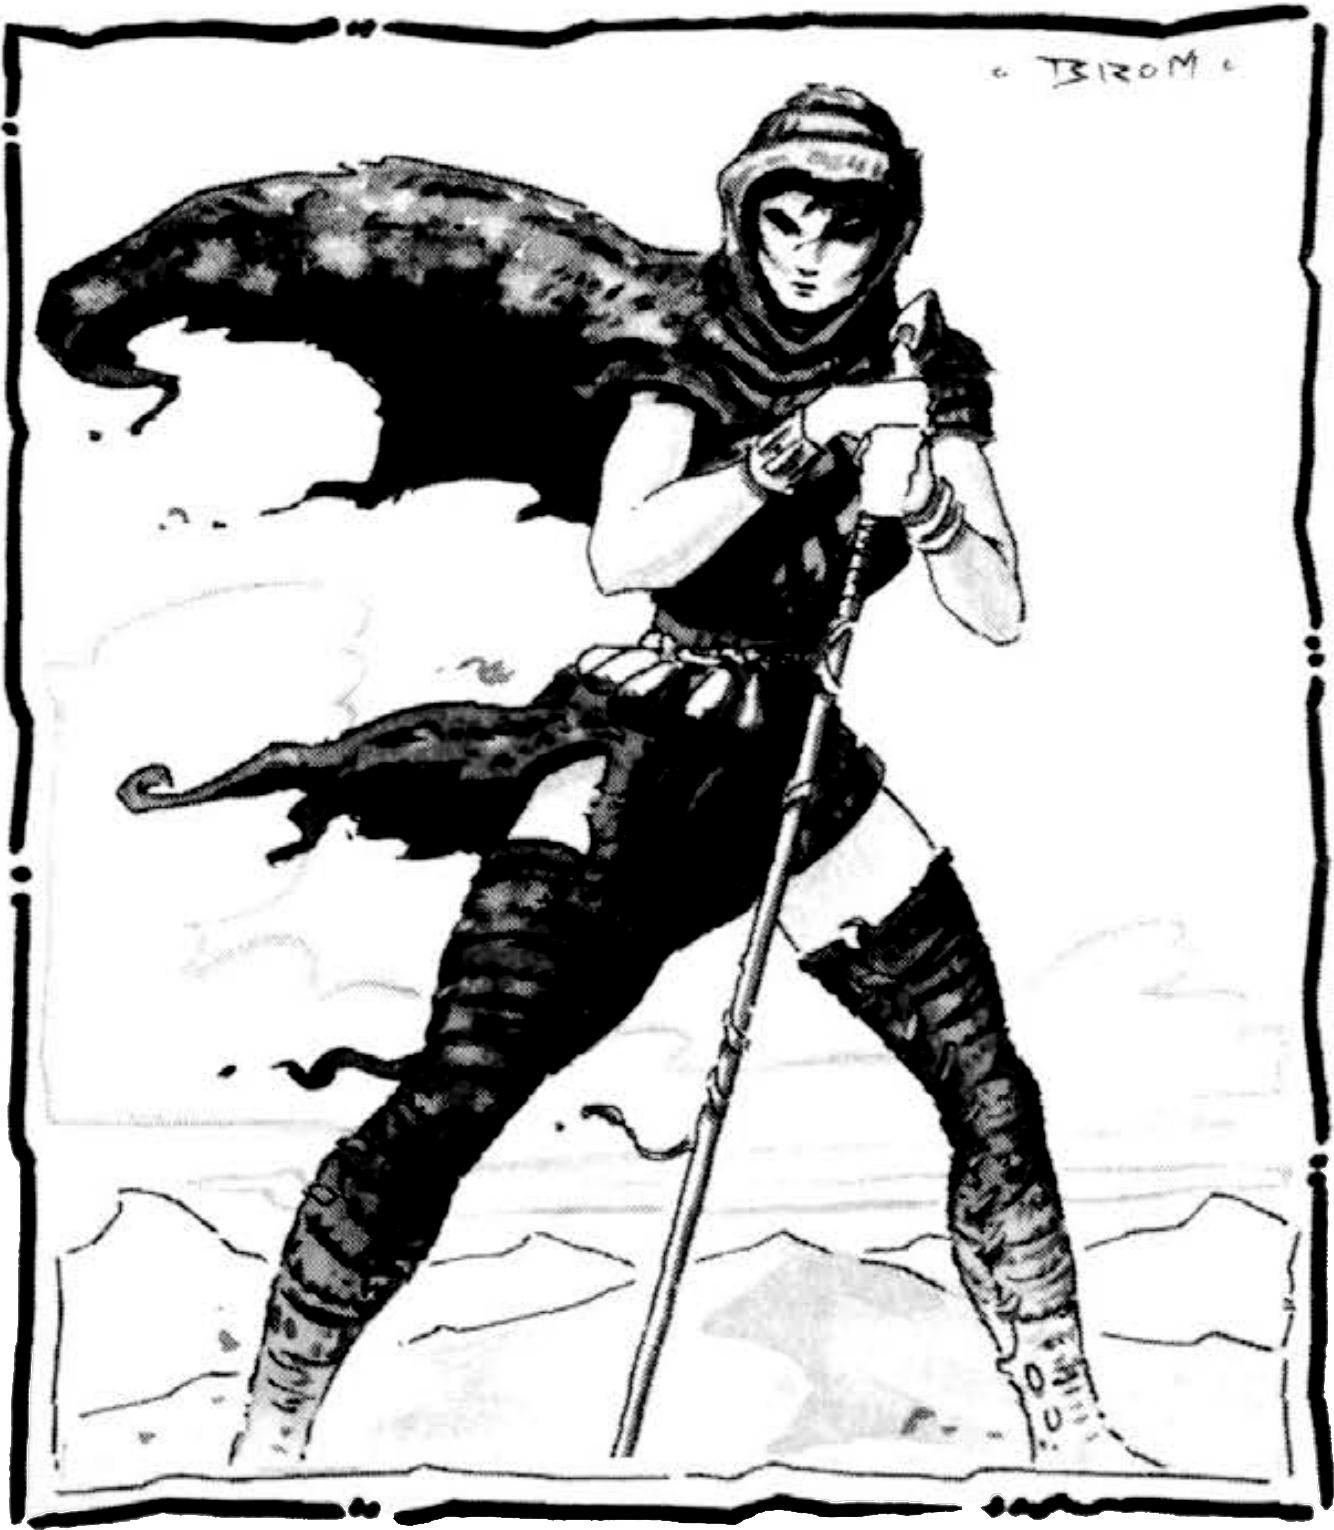
\includegraphics[width=\columnwidth]{images/halfelf-1.png}
\end{figure}
Unlike the parents of muls, elves and humans are often attracted to each other. Half-elves are typically the unwanted product of a casual interracial encounter.

\textbf{Personality:} Half-elves are notorious loners. Many Athasians believe that half-elves combine the worst traits of both races, but the most difficult aspect of half-elves---their lack of self-confidence comes not from their mixed origins but rather from a life of rejection from both parent races. Half-elves try in vain to gain the respect of humans or elves.

\textbf{Physical Description:} Averaging over 1.8 meters tall, half-elves combine Elven dexterity with human resilience. Bulkier than elves, most half-elves find it easier to pass themselves off as full humans than as full elves, but all have some features that hint at their Elven heritage.

\textbf{Relations:} Humans distrust the half-elf's Elven nature, while elves have no use for their mixed-blood children; Elven traditions demand that such children be left behind. Human society gives half-elves have a better chance of survival, but even less kindness. Half-elves sometimes find friendship among muls or even Thri-kreen. Half-elves will cooperate with companions when necessary, but find it difficult to rely on anyone. Many half-elves also turn to the animal world for company, training creatures to be servants and friends. Ironically, the survival skills and animal affinity that half-elves developed to cope with isolation make them valuable beast handlers in human society.

\textbf{Alignment:} Lawful and neutral half-elves labor for acceptance from a parent race, while chaotic ones have given up on acceptance, electing instead to reject the society that has rejected them.

\textbf{Half-Elven Lands:} Despite their unique nature, half-elves don't form communities. The few half-elves that settle down tend to live among humans who, unlike elves, at least find a use for them.

\textbf{Magic:} Half-elves often take up arcane studies, because it is a solitary calling.

\textbf{Psionics:} Mastery of the Way often provides the independence and self-knowledge that half-elves seek, and membership in a psionic academy can provide the half-elf with acceptance.

\textbf{Religion:} Because of their alienation from society and their affinity with animals, half-elves make excellent druids. Some half-elves turn their resentment of society into a profession and become sullen, bullying templars. As clerics, they are drawn to water's healing influence.

\textbf{Language:} Half-elves all speak the Common tongue. A few half-elves pick up the Elven language.

\textbf{Names:} Half-elves nearly always have human names. Unable to run as elves, they never receive Elven given names, or acceptance in an Elven tribe that they could use as surname.

\textbf{Adventurers:} In a party, half-elves often seem detached and aloof.

\subsection{Half-Elf Society}
Unlike other races, half-elves do not consider themselves a separate race, and, with very few exceptions, do not try to form half-Elven communities. A half-elf's life is typically harder than either a human's or an elf's. It is difficult for half-elves to find acceptance within either Elven or human society. Elves have not tolerance for those of mixed heritage, while humans do not trust their Elfish side. On the whole, humans are far more tolerant of half-elves than elves, who often refuse to allow such children into their tribes, and are likely to cast the half-elf's mother from the tribe as well.

Most half-elves consider themselves outsiders to all society and tend to wander throughout their entire lives, going through life as an outsider and loner. Half-elves are forced to develop a high level of self-reliance. Most half-elves take great pride in their self-reliance, but this pride often makes half-elves seem aloof to others. For many half-elves the detachment is a defensive mechanism to deal with a desire for acceptance from either human or Elven society that will likely never come. Some half-elves turn to the animal world for company, training creatures to be servants and friends.

\subsection{Roleplaying Suggestions}
Desperate for the approval of either elves or humans, you are even more desperate to appear independent and self-reliant, to cover your desire for approval. As a result, you tend towards a feisty, insecure, sullen self-reliance, refusing favors. You take every opportunity to show off your skills in front of elves and humans, but if an elf or a human were to actually praise you, you would probably react awkwardly or suspiciously. From your childhood, your closest friendships have been with animals. Other half-elves do not interest you. As time goes by and you learn from experience, you will find that you can also get along with other races neither human nor Elven: dwarves, pterran, muls, even thri-kreen. You don't feel the terrible need for their approval, and yet they give it more readily.

\subsection{Half-Elf Racial Traits}
\begin{itemize*}
    \item +2 Dexterity, $-2$ Charisma: Half-elves are limber like their Elven parents, but their upbringing leaves them with a poor sense of self, and affects their relations with others.
    \item Humanoid (elf): Half-elves are humanoid creatures with the elf subtype.
    \item Medium: As Medium creatures, half-elves have no bonuses or penalties due to size.
    \item Half-elf base land speed is 9 meters.
    \item Low-Light Vision: A half-elf can see twice as far as a human in starlight, moonlight, torchlight, and similar conditions of poor illumination. She retains the ability to distinguish color and detail under these conditions..
    \item Half-elves gain a +2 racial bonus to \skill{Disguise} checks when impersonating elves or humans.
    \item +1 racial bonus on \skill{Listen}, \skill{Search} and \skill{Spot} checks. Half-elves have keen senses, but not as keen as those of an elf.
    \item +2 racial bonus on all \skill{Survival} and \skill{Handle Animal} checks. Half-elves spend a lot of time in the wilds of the tablelands.
    \item Elven Blood: For all effects related to race, a half-elf is considered an elf. Half-elves, for example, are just as vulnerable to effects that affect elves as their elf ancestors are, and they can use magic items that are only usable by elves.
    \item Automatic Languages: Common and Elven. Bonus Languages: Any.
    \item Favored Class: Any. When determining whether a multiclass half-elf takes an experience point penalty, his highest-level class does not count when determining whether he takes an experience point for multiclassing.
\end{itemize*}
\section{Half-Giants}
\Quote{Mind of a child, strength of three grown men. I've seen a half-giant tear the walls out of a building because he wanted a better look at the tattoos on a mul inside.}{Daro, human trader}

Legend has it that in ages past, a sorcerer-queen used wizardry to beget a union of giant and human in order to create a race of powerful slaves. Whatever the truth of this legend, the half-giant race has increased in number and is now fairly common especially in human controlled lands near the shore of the Sea of Silt. Half-giants gain great strength, but dull wits, from their giant heritage, and are nearly as agile as their human forbearers.

\begin{figure}[t!]
\centering
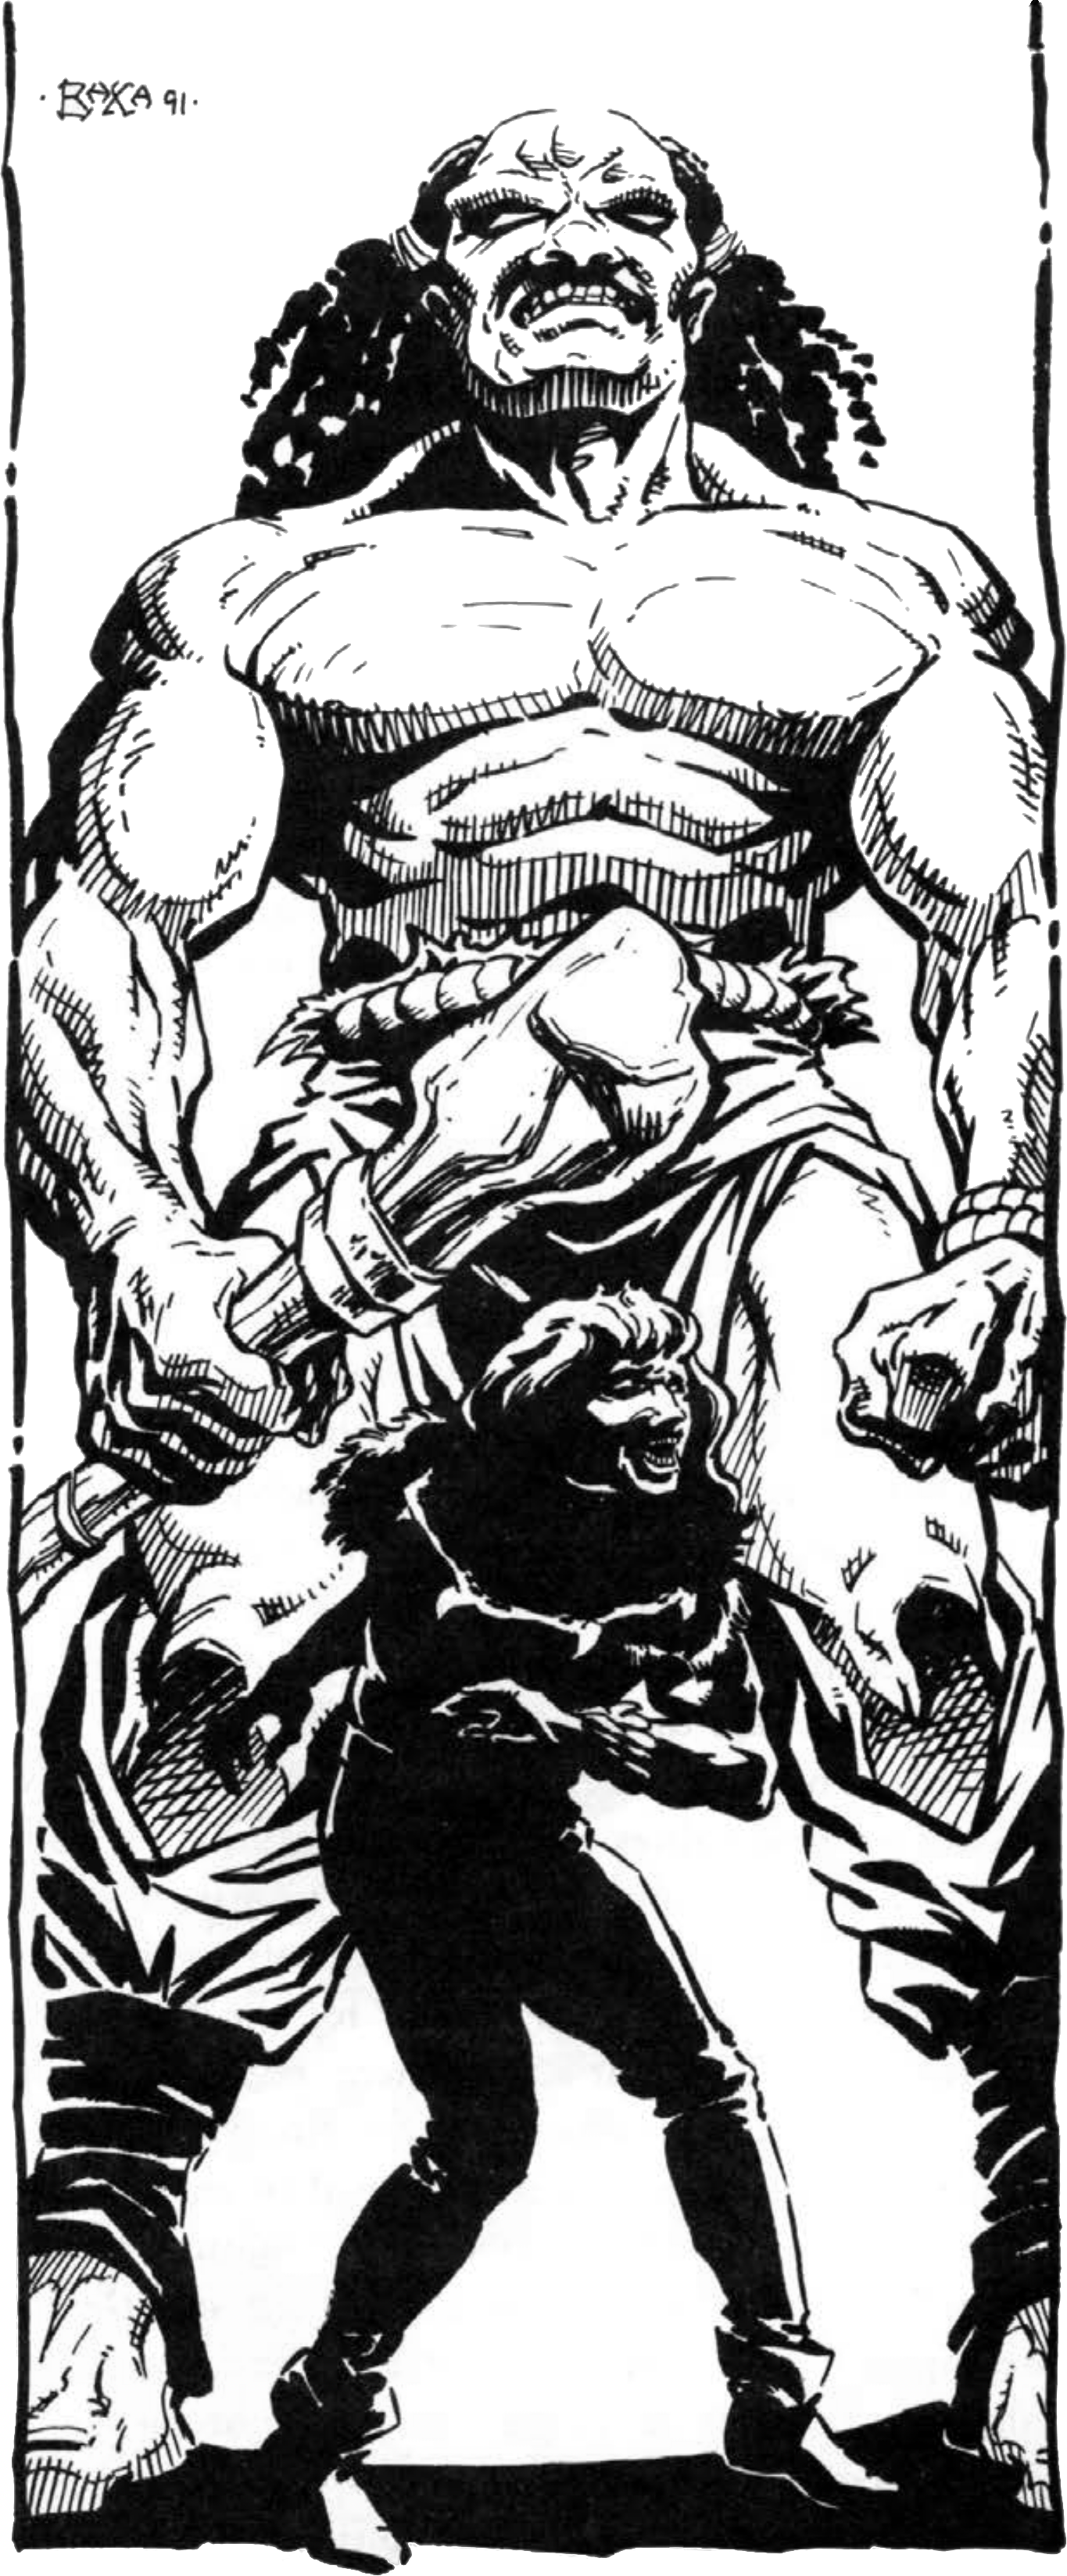
\includegraphics[width=\columnwidth]{images/halfgiant-1.png}
\WOTC
\end{figure}

\textbf{Personality:} Because of their artificial origins, there is no half-giant culture, tradition or homeland. Half-giants readily imitate the customs and cultures of their neighbors. Half-giants often display curiosity, a willingness to learn, and a general tendency towards kindness.

\textbf{Physical Description:} Physically, the half-giant is enormous, standing about 3.5 meters tall and weighing around 600 kg. Half-giants have thick hair, which is often kept braided (especially among females) or in a single tail that hangs behind the head and down the back. They dress in garb suitable to their occupation or environment. Half-giants mature at about 24 years of age and can live about 170 years.

\textbf{Relations:} The most powerful warriors on Athas, half-giants seem content to dwell in humanity's shadow. Half-giants tend to be friendly and eager to please, adopting the lifestyles, skills, and values of those they admire. A half-giant character who encounters a new situation looks around him to see what other people are doing. For example, a half-giant character that happens upon a Dwarven stone quarry may watch the dwarves, and then start quarrying stone himself. If he can make a living at it, he will continue to quarry stone just like his neighbor dwarves do; otherwise he will move on to something else.

\textbf{Alignment:} Half-giants can switch attitudes very quickly, taking on new values to fit new situations. A half-giant whose peaceful farming life is disrupted by marauders may soon adopt the morals of the renegades who sacked his village. A half-giant's nature is to switch his alignment aspect to imitate or otherwise react to a significant change around him.

\textbf{Half-Giant Lands:} Half-giants are most often found in the city-states, serving as gladiators, laborers, soldiers, and guards. A few half-giants collect into wilderness communities, often adopting the culture and customs of neighboring beings. The rare half-giant community often attaches itself to a charismatic or successful leader (not necessarily a half-giant) who demonstrates the tendencies they admire.

\textbf{Magic:} If a half-giant's companions accept wizardry, then the half-giant will also accept it. If a half-giant's companions hate wizardry, then the half-giant will be as eager as anyone to join in stoning a wizard. Among sophisticated companions who accept preserving magic but despise defiling magic, all but the brightest half-giants are likely to become confused, looking to their companions to see how they should react.

\textbf{Psionics:} While a single-classed half-giant psion is very rare, some half-giants take the path of the psychic warrior, becoming killing machines that can take apart a mekillot barehanded.

\textbf{Religion:} Half-giants do not display any affinity for the worship of one element over another.

\textbf{Language:} All half-giants speak the Common speech of slaves. Whatever tongue she speaks, the half-giant's voice is pitched so low as to occasionally be difficult to understand.

\textbf{Names:} Enslaved half-giants often have human names, and because of this they vary greatly. Free half-giants are likely to borrow the naming conventions of the race or people they are imitating at the time their child is born.

\textbf{Adventurers:} Half-giants are usually led to adventure by interesting companions of other races.

\subsection{Half-Giant Society}
A relatively young race, half-giants possess very little cultural identify of their own. Instead they adopt the customs and beliefs of those other cultures in which they live. Because of this, half-giants routinely change their alignment to match those around them who most influence them.
Half-giants can be found from one end of the Tablelands to the other, and often congregate in or near other population centers, absorbing the culture. Rarely do half-giants form communities of their own.

Unlike some other bastard races, half-giants can reproduce. A single off-spring is produced from half-giant unions after almost a year of pregnancy.

Though omnivorous, half-giants are tremendous consumers of water and food. They require twice the amount of food and water than humans. Clothing and equipment need twice the material to construct to fit a half-giant, leading to higher prices for half-giants.

Half-giants tend to damage objects and buildings around them through accidents of size alone. Some considerate half-giants camp outside city walls to avoid causing too much damage, but the draw of a city's culture and the below average intellect of most half-giants limits the number of half-giants who do so.

\subsection{Roleplaying Suggestions}
Always remember how much bigger and heavier you are than everyone else. Take advantage of your height in combat, but remember the disadvantages. Between your size and your lesser wits (even if you are a relatively intelligent half-giant people will assume you to be dull), you find yourself an object of comic relief. You are used to being teased and will endure more witty remarks than most people, but when you have been pushed too far your personality can suddenly shift, and you can unleash astonishing violence on your tormentors and any who stand in your way. Less frequently, these shifts can happen to you without provocation you just wake up with a different ethos and altered disposition.

Remember you are influenced by powerful personalities, and can shift your personality and ethics. You tend to imitate the tactics, clothes and demeanor of your ``little master.''
\subsection{Half-Giant Racial Traits}
\begin{itemize*}
    \item +8 Strength, +4 Constitution, $-2$ Dexterity, $-4$ Intelligence, $-4$ Wisdom, $-4$ Charisma: Half-giants are renowned for their great strength and dull wits.
    \item Large: As a Large creature, a half-giant takes a $-1$ penalty to Armor Class, a $-1$ penalty on attack rolls, and a $-4$ penalty on \skill{Hide} checks. She gains a +4 size bonus on grapple checks, and her lifting and carrying limits are double those of Medium characters, but she uses bigger weapons than humans use.
    \item Half-giants occupy a space of 3 meters and have a reach of 3 meters.
    \item Giant: Half-giants are creatures with the giant type.
    \item Half-giant base land speed is 12 meters.
    \item Darkvision: Half-giants can see in the dark out to 18 meters. Darkvision is black and white only, but it is otherwise like normal sight, and half-giants can function just fine with no light at all.
    \item Natural Armor: Half-giants have a +2 natural armor bonus to AC.
    \item Axis Alignment: One aspect of the half-giant's alignment must be fixed, and chosen during character creation. The other half must be chosen when they awake each morning. They are only bound to that alignment until they sleep again. For example, a half-giant may have a fixed lawful alignment. Every morning, he must choose to be lawful good, lawful neutral or lawful evil. This alignment change is not mandatory.
    \item Half-giants consume double the amount of food and water humans do.
    \item Favored Class: Barbarian. A multiclass half-giant's barbarian class does not count when determining whether he takes an experience point for multiclassing.
    \item Automatic Languages: Common. Bonus Languages: Dwarven, Gith, Giant. Half-giants will often pick up a race's tongue if imitating them long enough.
    \item Level Adjustment: +2. Half-giants are more powerful than the other races of the Tablelands and gain levels accordingly.
\end{itemize*}
\vskip6cm
\begin{figure*}[b!]
\centering
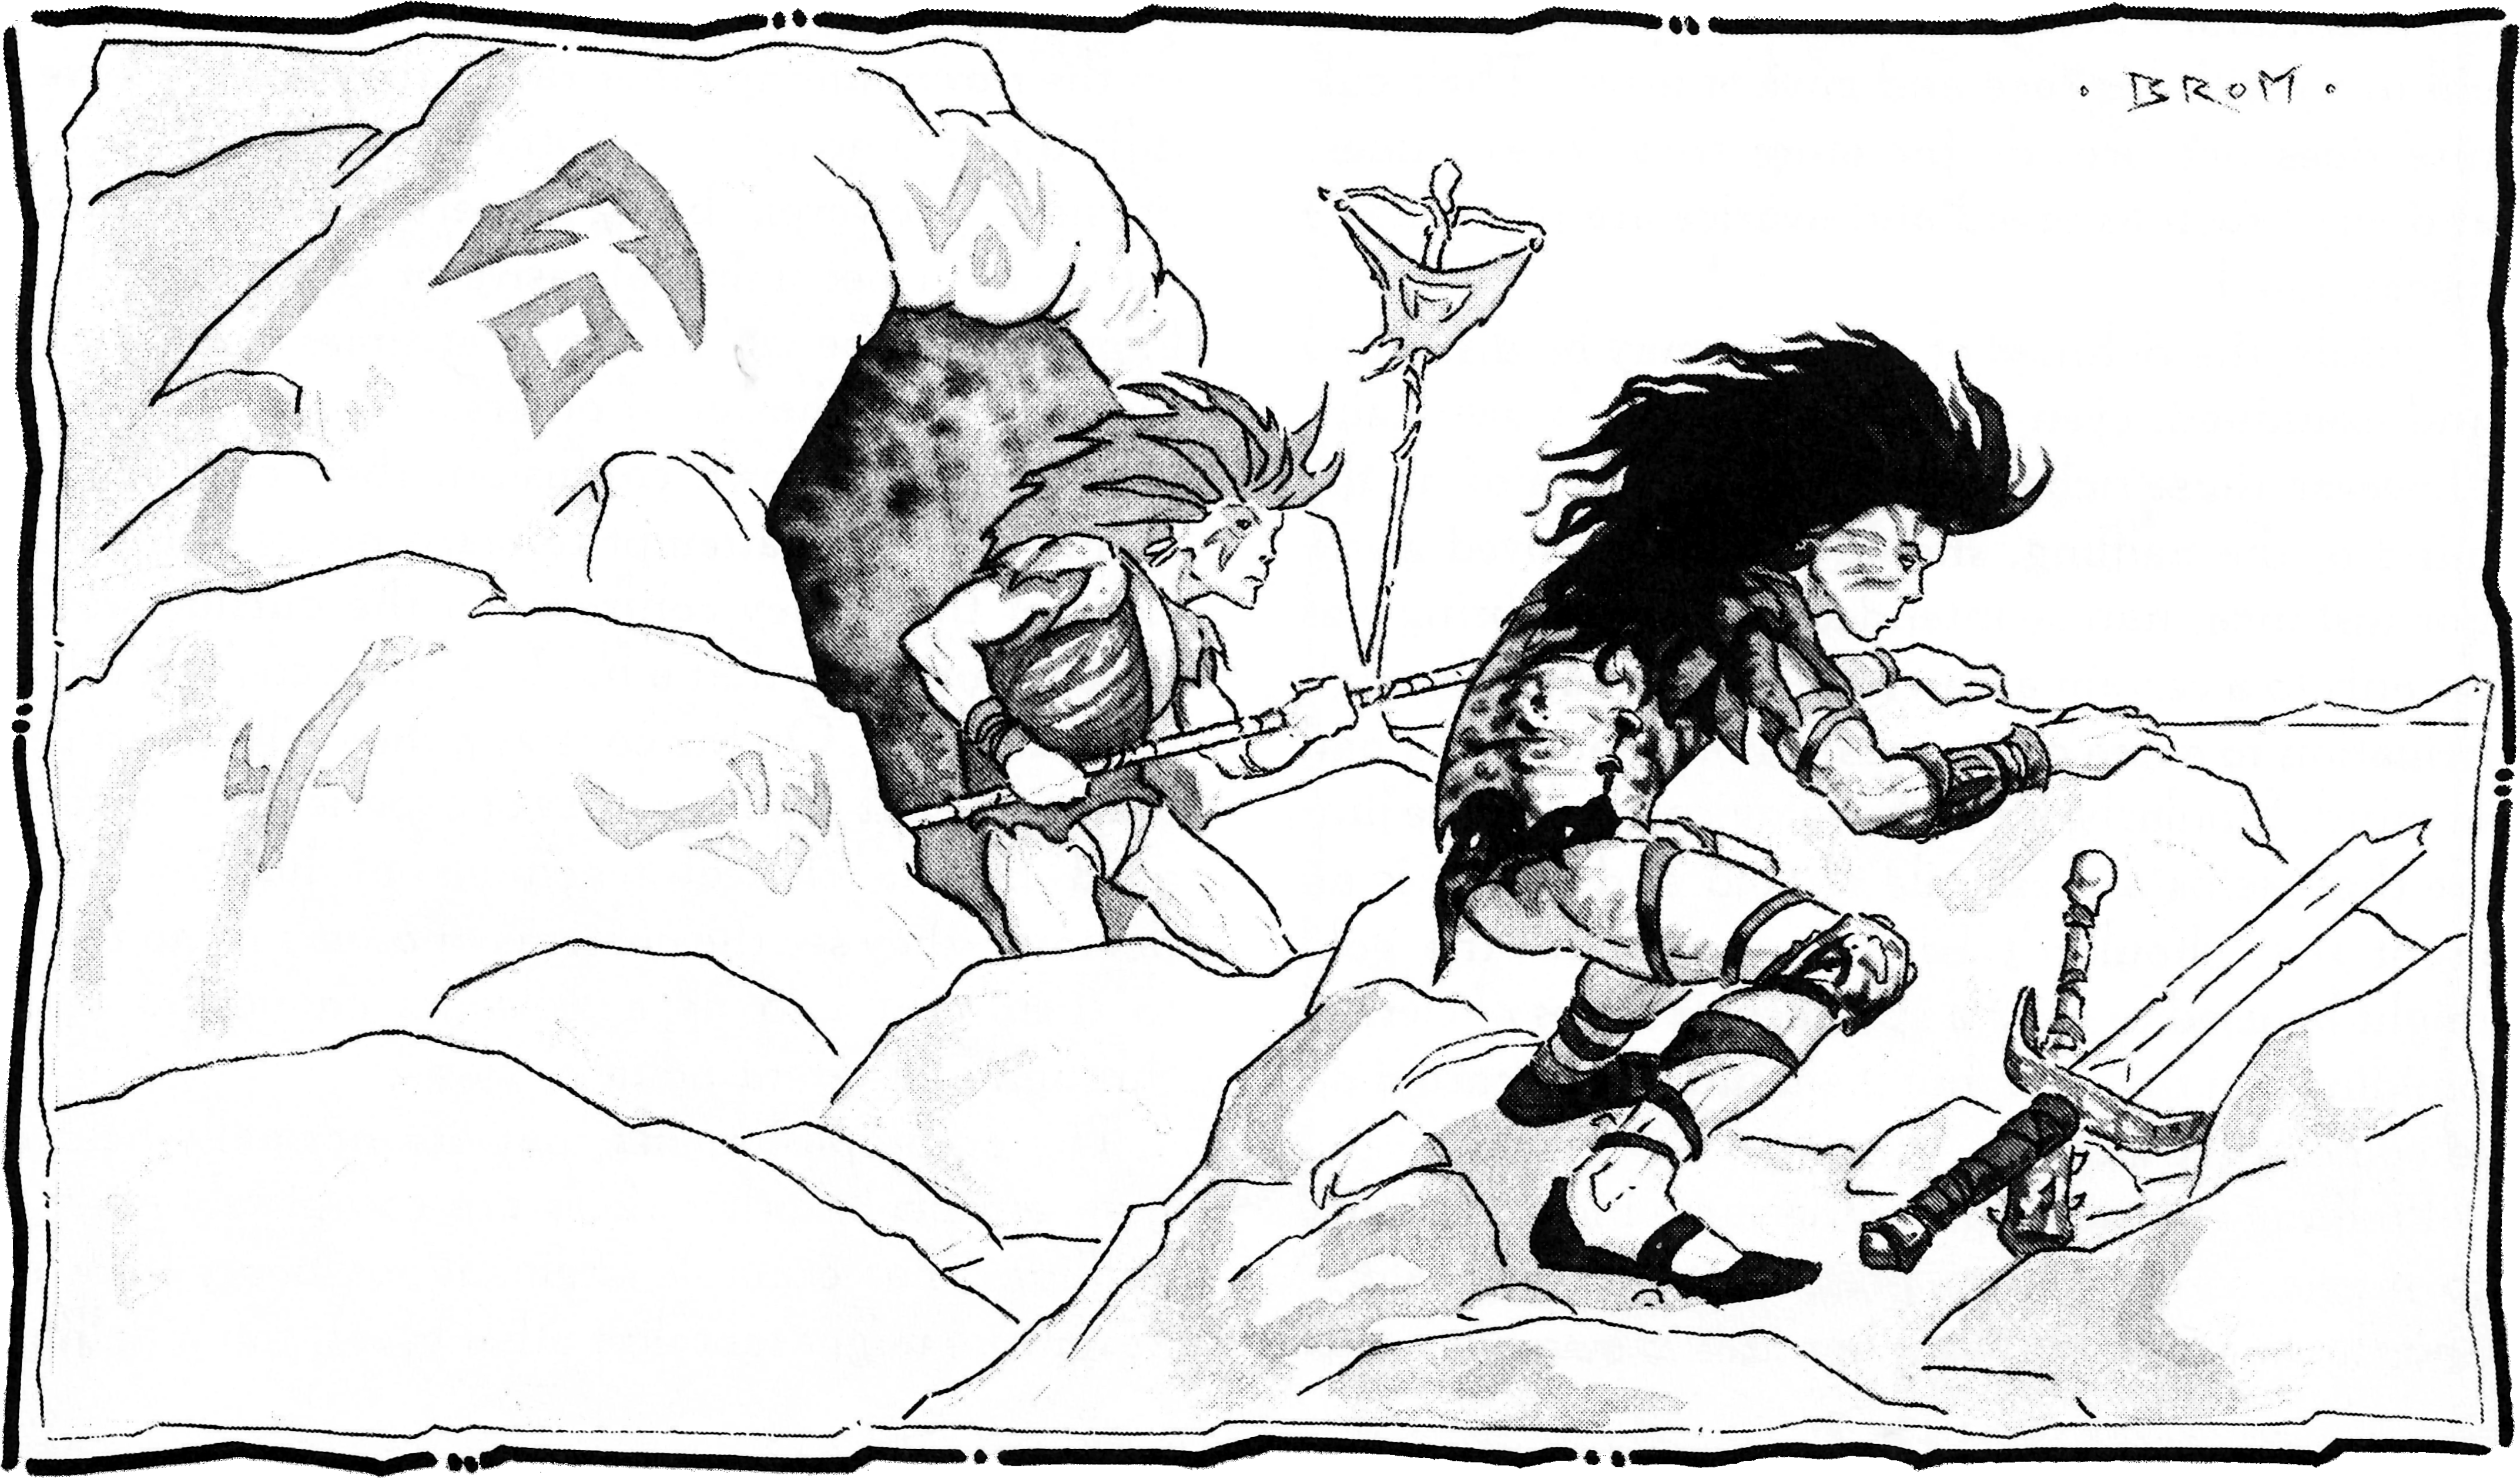
\includegraphics[width=\textwidth]{images/halfling-2.png}
\WOTC
\end{figure*}

\section{Halflings}
\Quote{Be wary of the forest ridge. The halflings who live there would as soon eat you alive as look at you. Chances are you won't even notice them until you've become the main course.}{Mo'rune, half-Elven ranger}

Halflings are masters of the jungles of the Ringing Mountains. They are small, quick and agile creatures steeped in an ancient and rich culture that goes back far into Athas' past. Although they are not common in the Tablelands, some halflings leave their homes in the forests to adventure under the{\tableheader Dark Sun}. As carnivores, halflings prefer to eat flesh raw.

\textbf{Personality:} Halflings have difficulty understanding others' customs or points of view, but curiosity helps some halflings overcome their xenophobia. Little concerned with material wealth, halflings are more concerned with how their actions will affect other halflings.

\textbf{Physical Description:} Halflings are small creatures, standing only about 1 meter tall and weighing 25 to 30 kilograms. Rarely affected by age, halfling faces are often mistaken for the faces of human children. They dress in loincloths, sometimes with a shirt or vest, and paint their skins with bright reds and greens. Forest halflings rarely tend to their hair, and some let it grow to great lengths, though it can be unkempt and dirty. They live to be about 120 years old.

\textbf{Relations:} Halfling's culture dominates their relations with others. They relate very well to each other, since they all have the same cultural traits and are able to understand each other. Halflings of different tribes still share a tradition of song, art and poetry, which serves as a basis of communication. Creatures that do not know these cultural expressions are often at a loss to understand the halfling's expressions, analogies and allusions to well-known halfling stories. Halflings can easily become frustrated with such ``uncultured'' creatures. They abhor slavery and most halflings will starve themselves rather than accept slavery.

\textbf{Alignment:} Halflings tend towards law and evil. Uncomfortable with change, halflings tend to rely on intangible constants, such as racial identity, family, clan ties and personal honor. On the other hand, halflings have little respect for the laws of the big people.

\textbf{Halfling Lands:} Halflings villages are rare in the tablelands. Most halflings live in tribes or clans in the Forest Ridge, or in the Rohorind forest west of Kurn. Many dwell in treetop villages. Non-halflings typically only see these villages from within a halfling cooking pot.

\textbf{Magic:} Many halfling tribes reject arcane magic. Tribes that accept wizards tend to have preserver chieftains. Only renegade halfling tribes are ever known to harbor defilers.

\textbf{Psionics:} Many halflings become seers or nomads. In the forest ridge, many tribal halflings become multiclassed seer/rangers, and become some of the deadliest trackers on Athas.

\textbf{Religion:} Halflings' bond with nature extends into most aspects of their culture. A shaman or witch doctor, who also acts as a spiritual leader, often rules their clans. This leader is obeyed without question. Halfling fighters willingly sacrifice themselves to obey their leader.

\textbf{Language:} Halflings rarely teach others their language, but some individuals of the Tablelands have learned the wild speech. Halflings found in the Tablelands often learn to speak Common.

\textbf{Names:} Halflings tend to have only one given name.

\textbf{Male Names:} Basha, Cerk, Derlan, Drassu, Entrok, Kakzim, Lokee, Nok, Pauk, Plool, Sala, Tanuka, Ukos, Zol.

\textbf{Female Names:} Alansa, Anezka, Dokala, Grelzen, Horga, Jikx, Joura, Nasaha, Vensa.

\textbf{Adventurers:} Exploring the Tablelands gives curious halflings the opportunity to learn other customs. Although they may at first have difficulty in understanding the numerous practices of the races of the Tablelands, their natural curiosity enables them to learn and interact with others. Other halflings may be criminals, renegades or other tribal outcasts, venturing into the Tablelands to escape persecution by other halflings.

\subsection{Halfling Society}
Most halflings have a common outlook on life that results in considerable racial unity across tribal and regional ties. Rarely will one halfling draw the blood of another even during extreme disagreements. Only renegade halflings do not share this racial unity, and are cast out of their tribes because of it.

Halfling society is difficult for other races to understand, as such concepts as conquest and plundering have no place. The most important value in halfling society is the abilities of the inner self as it harmonizes with the environment and the rest of the halfling race.

Halflings are extremely conscious of their environment. They are sickened by the ruined landscape of the Tyr region and desperately try to avoid having similar devastation occur to their homelands in the Forest Ridge. Most halflings believe that care must be taken to understand and respect nature and what it means to all life on Athas.

Halfling culture is expressed richly through art and song. Story telling in which oral history is passed on to the next generation is an important part of each halfling community. Halflings rely on this shared culture to express abstract thoughts and complicated concepts. This causes problems and frustration when dealing with non-halflings. Typically halflings assume that whomever they are talking to have the same cultural background to draw upon, and find it difficult to compensate for a listener who is not intimately familiar with the halfling history and ``lacks culture.''

Generally open-minded, wandering halflings are curious about outside societies and will attempt to learn all they can about other cultures. Never, will they adopt aspects of those cultures as their own, believing halfling culture to be innately superior to all others. Nor do they seek to change others' culture or views.

While halflings are omnivorous, they vastly prefer meat. Their meat heavy diet means that halflings view all living creatures, both humanoid and animal, as more food than equals. At the same time, most halflings believe that other races have the same perception of them. As a result, halflings are rarely likely to trust another member of any other race.

\subsection{Roleplaying Suggestions}
Remember to consistently take your height into account. Roleplay the halfling culture described above: eating opponents, treating fellow halflings with trust and kindness, suspicion of big people, and general lack of interest in money.

\subsection{Halfling Racial Traits}
\begin{itemize*}
    \item $-4$ Strength, +4 Dexterity, +4 Wisdom, $-2$ Charisma: Halflings are quick and stealthy, but weaker than humans.
    \item Humanoid (halfling): Halflings are humanoid creatures with the halfling subtype.
    \item Small: As a Small creature, a halfling gains a +1 size bonus to Armor Class, a +1 size bonus on attack rolls, and a +4 size bonus on \skill{Hide} checks, but she uses smaller weapons than humans use, and her lifting and carrying limits are three-quarters of those of a Medium character.%Halflings gain a +1 size bonus to Armor Class and a +1 size bonus on all attack rolls.
    \item Halfling base land speed is 6 meters.
    % \item Halflings receive a $-2$ penalty to all \skill{Diplomacy} skill checks when dealing with other races.
    \item +4 racial bonus on \skill{Climb} and \skill{Jump} checks: Halflings are agile.
    \item +2 racial bonus on saving throws against spells and spell-like effects.
    \item +1 racial attack bonus with a thrown weapon: javelins and slings are common weapons in feral halfling society, and many halflings are taught to throw at an early age.
    \item Halflings get advantage on \skill{Listen} checks---they have keen ears. Their senses of smell and taste are equally keen; they get advantage to all Wisdom checks that assess smell or taste.
    \item Halfings consume half the amount of food and water humans do.
    \item Automatic Languages: Halfling. Bonus Languages: Common, Dwarven, Elven, Gith, Kreen, Rhul-thaun, Sylvan, and Yuan-ti.
    \item Favored Class: Druid, Ranger, or Rogue. A halfling must choose between druid, ranger, or rogue as favored class. This choice cannot be changed. A multiclass halfling's chosen class does not count when determining whether he takes an experience point for multiclassing.
    \item Level Adjustment: +1.
\end{itemize*}
\section{Muls}
\Quote{See, the trick is to break their will. Not too much, mind you. Nobody wants to watch a docile gladiator, and muls are too expensive to waste as labor slaves. But, you don't want them trying to escape every other day. Would you like to tell the arena crowd that their favorite champion will not be appearing in today's match because he died trying to escape your pens?}{Gaal, Urikite arena trainer}

Born from the unlikely parentage of dwarves and humans, muls combine the height and adaptable nature of humans with the musculature and resilience of dwarves. Muls enjoy traits that are uniquely their own, such as their robust metabolism and almost inexhaustible capacity for work. The hybrid has disadvantages in a few areas as well: sterility, and the social repercussions of being created for a life of slavery. Humans and dwarves are not typically attracted to each other. The only reason that muls are so common in the Tablelands is because of their value as laborers and gladiators: slave-sellers force-breed humans and dwarves for profit. While mul-breeding practices are exorbitantly lucrative, they are often lethal to both the mother and the baby. Conception is difficult and impractical, often taking months to achieve. Even once conceived, the mul takes a full twelve months to carry to term; fatalities during this period are high. As likely as not, anxious overseers cut muls from the dying bodies of their mothers.

\textbf{Personality:} All gladiators who perform well in the arenas receive some degree of pampered treatment, but muls receive more pampering than others. Some mul gladiators even come to see slavery as an acceptable part of their lives. However, those that acquire a taste of freedom will fight for it. Stoic and dull to pain, muls are not easily intimidated by the lash. Masters are loath to slay or maim a mul who tries repeatedly to escape, although those who help the mul's escape will be tormented in order to punish the mul without damaging valuable property. Once a mul escapes or earns his freedom, slavery remains a dominant part of his life. Most muls are heavily marked with tattoos that mark his ownership, history, capabilities and disciplinary measures. Even untattooed muls are marked as a potential windfall for slavers: it is clearly cheaper to ``retrieve'' a mul who slavers can claim had run away, than to start from scratch in the breeding pits.

\begin{figure}[t!]
\centering
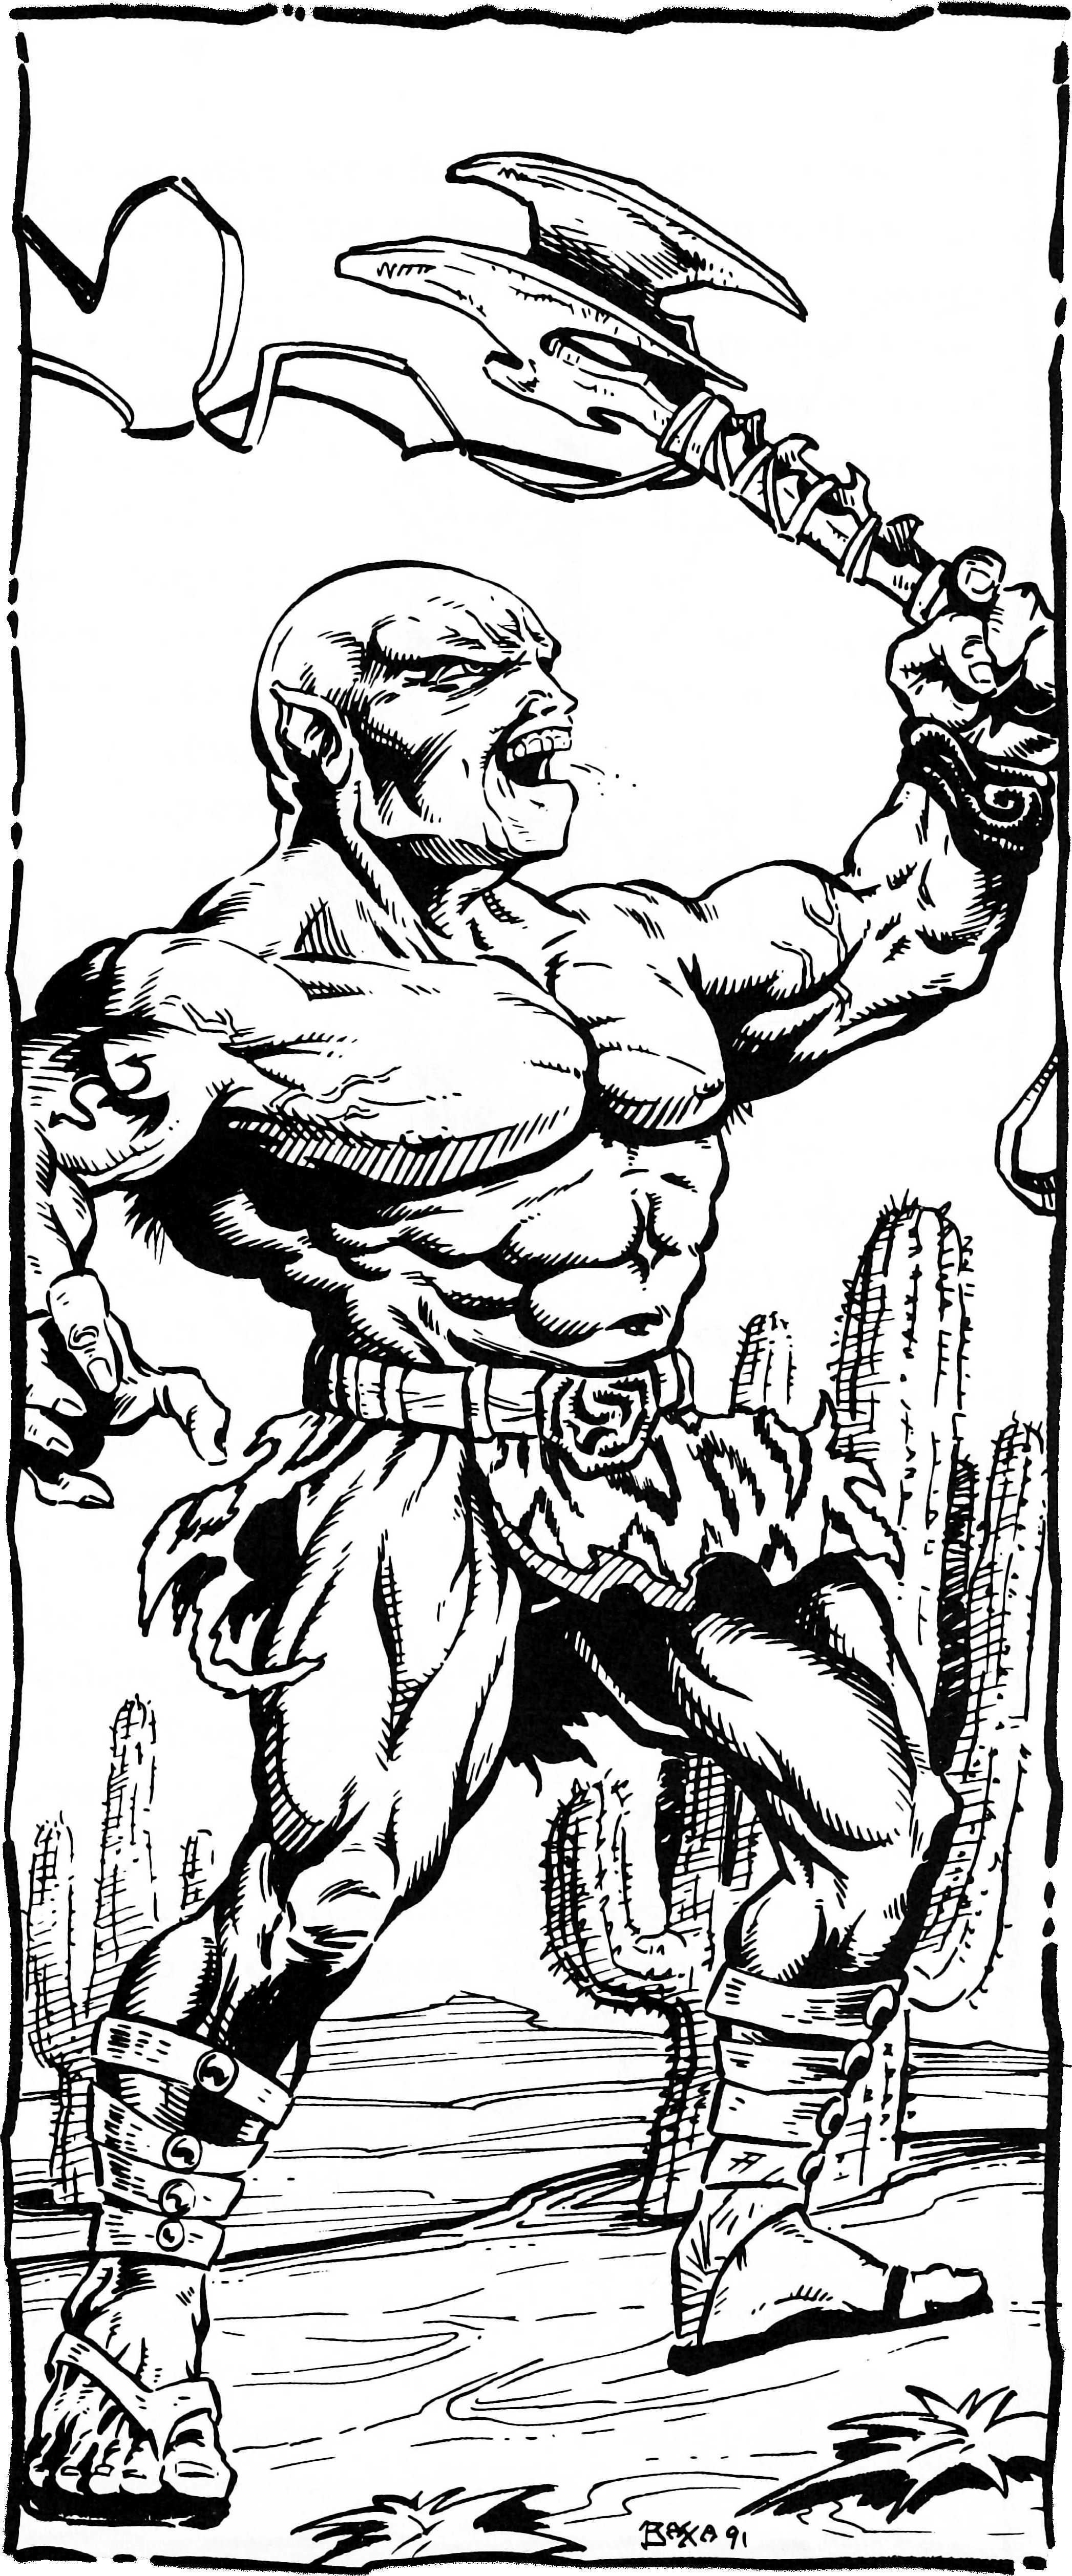
\includegraphics[width=\columnwidth]{images/mul-1.png}
\WOTC
\end{figure}

\textbf{Physical Description:} Second only to the half-giant, the mul is the strongest of the common humanoid races of the tablelands. Muls grow as high as 2.1 meters, weighing upwards of 125 kilograms, but carry almost no fat at all on their broad muscular frames. Universal mul characteristics include angular, almost protrusive eye ridges, and ears that point sharply backwards against the temples. Most muls have dark copper-colored skin and hairless bodies.

\textbf{Relations:} Most mul laborers master the conventions of slave life, figuring out through painful experience who can be trusted and who cannot. (Muls learn from their mistakes in the slave pits to a greater extent than other races not because they are cleverer, but because unlike slaves of other races they tend to survive their mistakes, while other slave races are less expensive and therefore disposable. Only the most foolish and disobedient mul would be killed. Most masters will sell a problem mul slave rather than kill him.) Their mastery of the rules of slave life and their boundless capacity for hard work allows them to gain favor with their masters and reputation among their fellow slaves.

\textbf{Alignment:} Muls tend towards neutrality with respect to good and evil, but run the gamut with respect to law or chaos. Many lawful muls adapt well to the indignities of slavery, playing the game for the comforts that they can win as valued slaves. A few ambitious lawful muls use the respect won from their fellow-slaves to organize rebellions and strike out for freedom. Chaotic muls, on the other hand, push their luck and their value as slaves to the breaking point, defying authority, holding little fear for the lash.

\textbf{Mul Lands:} As a collective group, muls have no lands to call their own. Occasionally, escaped muls band together as outlaws and fugitives, because of their common ex-slave backgrounds, and because their mul metabolism makes it easier for them to survive as fugitives while other races cannot keep up. Almost without exception, muls are born in the slave pits of the merchants and nobles of the city-states. Most are set to work as laborers, some as gladiators, and fewer yet as soldier-slaves. Very few earn their freedom, a greater number escape to freedom among the tribes of ex-slave that inhabit the wastes.

\textbf{Magic:} Muls dislike what they fear, and they fear wizards. They also resent that a wizard's power comes from without, with no seeming effort on the wizard's part, while the mul's power is born of pain and labor. Mul wizards are unheard of.

\textbf{Psionics:} Since most slave owners take steps to ensure that their property does not get schooled in the Way, it is rare for a mul to receive any formal training. Those that get this training tend to excel in psychometabolic powers.

\textbf{Religion:} Even if muls were to create a religion of their own, as sterile hybrids, they would have no posterity to pass it on to. Some cities accept muls as templars. Mul clerics tend to be drawn towards the strength of elemental earth.

\textbf{Language:} Muls speak the Common tongue of slaves, but those favored muls that stay in one city long enough before being sold to the next, sometimes pick up the city language. Because of their tireless metabolism, muls have the capacity to integrate with peoples that other races could not dream of living with, such as elves and Thri-kreen.

\textbf{Names:} Muls sold as laborers will have common slave names. Muls sold as gladiators will often be given more striking and exotic names. Draji names (such as Atlalak) are often popular for gladiators, because of the Draji reputation for violence. Masters who change their mul slaves' professions usually change their names as well, since it is considered bad form to have a gladiator with a farmer's name, and a dangerous incitement of slave rebellions to give a common laborer the name of a gladiator.

\textbf{Adventurers:} Player character muls are assumed to have already won their freedom. Most freed mul gladiators take advantage of their combat skills, working as soldiers or guards. Some turn to crime, adding rogue skills to their repertoire. A few muls follow other paths, such as psionics, templar orders or elemental priesthoods.

\subsection{Mul Society}
Muls have no racial history or a separate culture. They are sterile and cannot reproduce, preventing them from forming family groups and clans. The vast majority of muls are born in slavery, through breeding programs. Often the parents resent their roles in the breeding program and shun the child, leaving the mul to a lonely, hard existence. The taskmaster's whip takes the place of a family. For these reasons, many muls never seek friends or companionship, and often have rough personalities with tendencies towards violence.

The mul slave trade is very profitable, and thus the breeding programs continue. A slave trader can make as much on the sale of a mul as he could with a dozen humans. As slaves, a mul has his profession selected for him and is given extensive training as he grows.

Mul gladiators are often very successful, and win a lot of money for their owners. Highly successful gladiators are looked after by their owners, receiving a large retinue of other slaves to tend to their whims and needs. This has lead to the expression, ``pampered like a mul,'' being used often by the common folk.

Muls not trained as gladiators are often assigned to hard labor and other duties that can take advantage of the mul's hardy constitution and endurance.

\subsection{Roleplaying Suggestions}
Born to the slave pens, you never knew love or affection; the taskmaster's whip took the place of loving parents. As far as you have seen, all of life's problems that can be solved are solved by sheer brute force. You know to bow to force when you see it, especially the veiled force of wealth, power and privilege. The noble and templar may not look strong, but they can kill a man with a word. You tend towards gruffness. In the slave pits, you knew some muls that never sought friends or companionship, but lived in bitter, isolated servitude. You knew other muls who found friendship in an arena partner or co-worker. You are capable of affection, trust and friendship, but camaraderie is easier for you to understand and express - warriors slap each other on the shoulder after a victory, or give their lives for each other in battle. You don't think of that sort of event as ``friendship'' - it just happens.

\subsection{Mul Racial Traits}
\begin{itemize*}
    \item +4 Strength, +2 Constitution, $-2$ Intelligence, $-4$ Charisma: Combining the human height with the Dwarven musculature, muls end up stronger than either parent race, but their status as born-to-be slaves makes them insecure in their dealings with others.
    \item Humanoid (dwarf): Muls are humanoid creatures with the dwarf subtype.
    \item Medium: As Medium creatures, muls have no bonuses or penalties due to size.
    \item Mul base land speed is 9 meters.
    % \item Darkvision: Muls can see in the dark up to 9 meters. Darkvision is black and white only, but is otherwise like normal sight, and muls can function just fine with no light at all.
    \item Muls have +2 racial bonus on his damage rolls with light or thrown weapons (including unarmed strikes).
    \item Extended Activity: Muls require double the amount of time before making any check related to endurance.
    \begin{itemize*}
        \item Muls need to sleep every two days (but may choose to sleep every day);
        \item Muls can walk for 16 hours before beginning a forced march;
        \item Muls can hold their breath or run for a number of rounds equal to four times their Constitution score;
        \item Muls can go without food for six days;
        \item Muls can go without water for two days plus a number of hours equal to twice their Constitution score;
        \item Muls make Constitution checks every two hours of marching beyond 16 hours;
        \item Muls make Constitution checks every two rounds to continue holding their breath or running;
        \item Muls make Fortitude checks every two hours in a very hot (32 °C to 42 °C) or very cold ($-17$ °C to 4 °C) environments, every 20 minutes in severe heat (43 °C to 60 °C) or severe cold ($-28$ °C to $-18$ °C), and every 10 minutes in extreme heat \hskip10cm (61 °C to 82 °C), extreme cold ($-45$ °C to $-29$ °C), or worse environments;
        \item Muls make Constitution checks every two days after the first period without food;
        \item Muls make Constitution checks every two hours after the first period without water.
    \end{itemize*}
    % \item Tireless: Muls get a +4 racial bonus to checks for performing a physical action that extends over a period of time (running, swimming, holding breath, and so on). This bonus stacks with the \feat{Endurance} feat. This bonus may also be applied to savings throws against spells and magical effects that cause weakness, fatigue, exhaustion or enfeeblement.
    % \item Extended Activity: Muls may engage in up to 12 hours of hard labor or forced marching without suffering from the associated nonlethal damage and fatigue.
    \item Dwarven Blood: For all effects related to race, a mul is considered a dwarf. Muls, for example, are just as vulnerable to effects that affect dwarves as their dwarf ancestors are, and they can use magic items that are only usable by dwarves.
    % \item Nonlethal Damage Resistance 1/--. Muls are difficult to subdue, and do not notice minor bruises, scrapes, and other discomforts that pain creatures of other races.
    \item Favored Class: Fighter or Gladiator. A mul must choose between fighter or gladiator as favored class. This choice cannot be changed. A multiclass mul's chosen class does not count when determining whether he takes an experience point for multiclassing.
    \item Automatic Language: Common. Bonus Languages: Dwarven, Elven, Gith, and Giant.
    \item Level Adjustment: +1.
\end{itemize*}
% \section{Pterrans}
\Quote{The people of the Tablelands know nothing of life. They choose no Path for themselves, and consume everything until they are dead.}{Keltruch, pterran ranger}

\begin{figure}[b!]
\centering
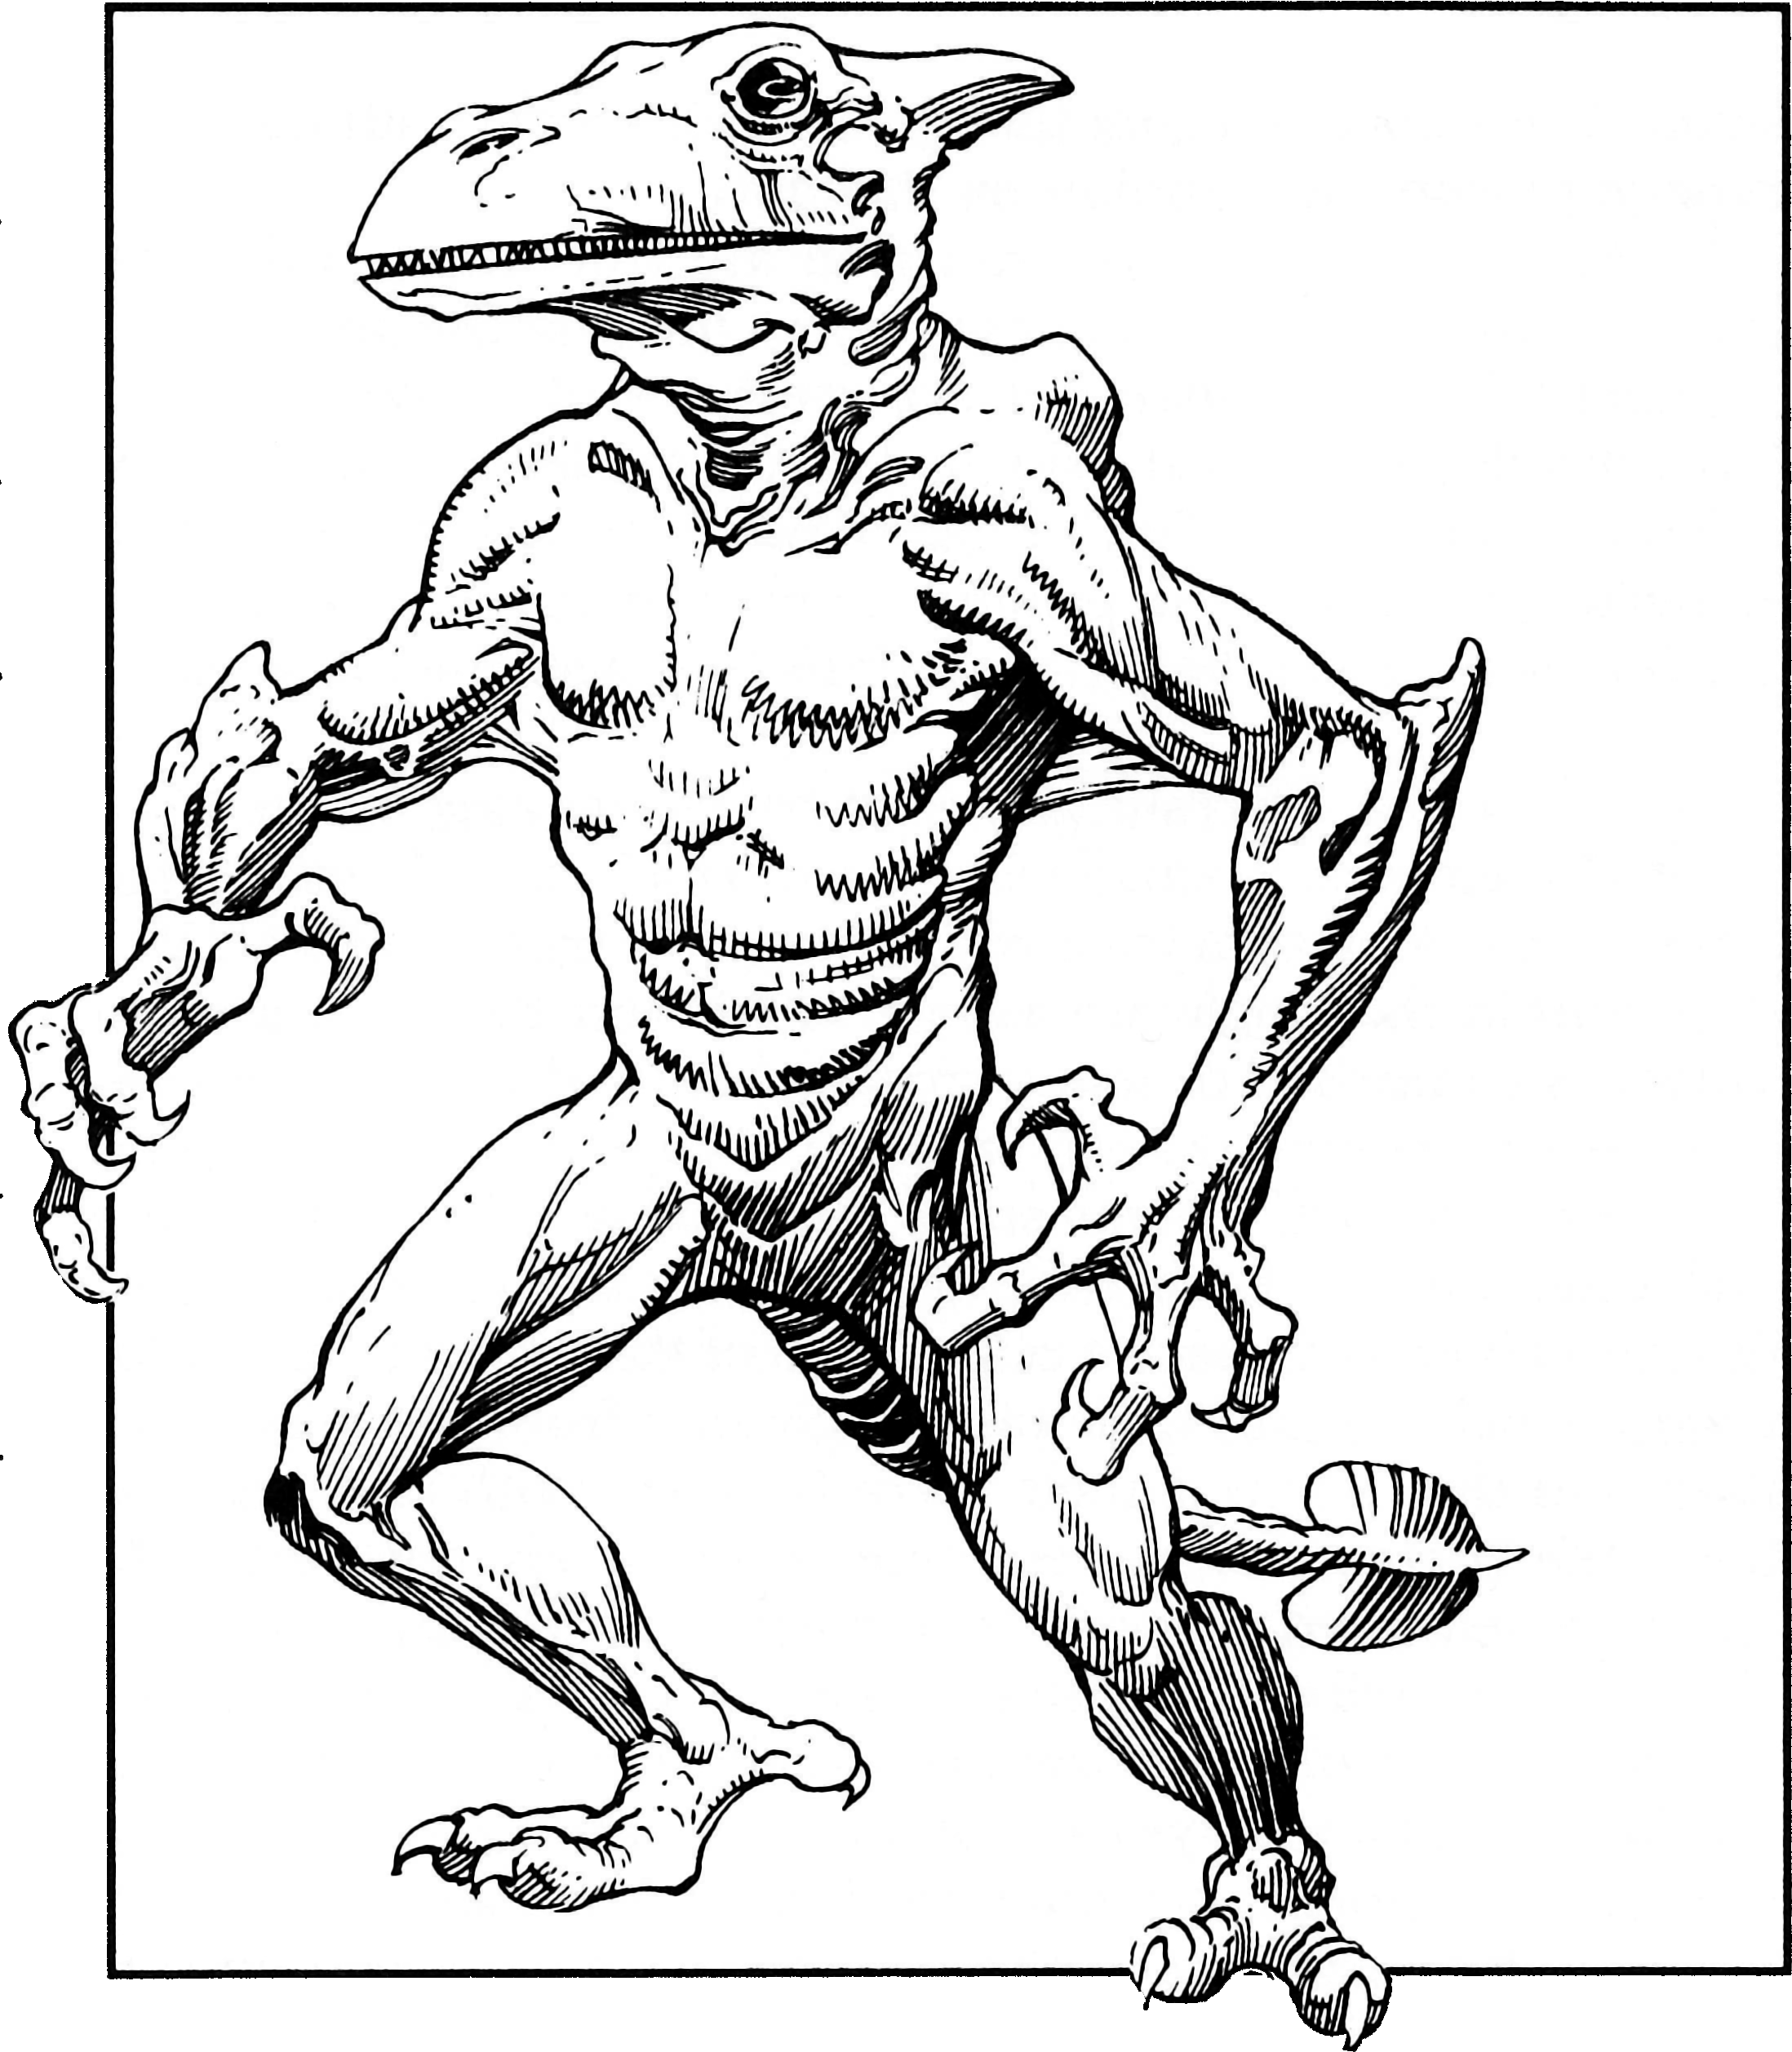
\includegraphics[width=\columnwidth]{images/pterran-1.png}
\end{figure}

Pterrans are rarely seen in the Tablelands. They live their lives in the Hinterlands, rarely leaving the safety of their villages. However, the recent earthquake and subsequent storms have brought disruption into the pterran's lives. More pterrans now venture outside their homes, and come to the Tyr region to seek trade and information.

\textbf{Personality:} Among strangers, pterrans seem like subdued, cautious beings, but once others earn a pterran's trust, they will find an individual that is open, friendly, inquisitive, and optimistic. In other respects, a pterran's personality is largely shaped by her chosen life path: Pterrans who choose the path of the warrior are less disturbed by the brutality of the Tablelands; they are constantly examining their surroundings and considering how the terrain where they are standing could be defended; they take greatest satisfaction from executing a combat strategy that results in victory without friendly casualties. Pterrans who choose the path of the druid are most interested in plants, animals, and the state of the land; they take greatest satisfaction when they eliminate a threat to nature. Pterrans that choose the path of the mind are most interested in befriending and understanding other individuals and societies; these telepaths take greatest satisfaction from intellectual accomplishments such as solving mysteries, exposing deception, resolving quarrels between individuals, and establishing trade routes between communities.

\textbf{Physical Description:} Pterrans are 1.5 to 1.9 meters tall reptiles with light brown scaly skin, sharp teeth, and a short tail. Pterrans wear little clothing, preferring belts and loincloths, or sashes. They walk upright, like humanoids, and have opposing thumbs and three-fingered, talon-clawed hands. Pterrans have two shoulder stumps, remnants of wings they possessed long ago, and a finlike growth juts out at the back of their heads. Pterrans weigh between 90 to 110 kilograms. There is no visible distinction between male and female pterrans.

\textbf{Relations:} Pterrans are new to the Tablelands, and unaccustomed to cultures and practices of the region. They have learned to not judge too quickly. Their faith in the Earth Mother means they undertake their adventure with open minds, but they will remain subdued and guarded around people they do not trust. A pterran's respect for the Earth Mother governs all his behavior. Creatures that openly destroy the land or show disrespect for the creatures of the wastes are regarded suspiciously. Pterrans understand the natural cycle of life and death, but have difficulty with some aspects of the city life, such as cramped living spaces, piled refuse, and the smells of unwashed humanoids.

\textbf{Alignment:} Pterrans tend towards lawful, well-structured lives, and most of them are good. Evil pterran adventurers are usually outcasts who have committed some horrible offense.

\textbf{Pterran Lands:} Most adventuring pterrans come from one of two villages in the Hinterlands, southwest of the Tyr regions: Pterran Vale and Lost Scale.

\textbf{Magic:} The wizard's use of the environment as a source of power conflicts with a pterran's religious beliefs. Pterrans will cautiously tolerate members of other races who practice preserving magic, if the difference is explained to them.

\textbf{Psionics:} Virtually all pterrans have a telepathic talent, and pterran psions are nearly universally telepaths. Telepathy is considered one of the honored pterran ``life paths.''

\textbf{Religion:} Pterrans worship the Earth Mother, a representation of the whole world of Athas. Their devotion to the Earth Mother is deeply rooted in all aspects of their culture, and it defines a pterran's behavior. All rituals and religious events are related to their worship of the Earth Mother. Religious events include festivals honoring hunts or protection from storms, with a priest presiding over the celebration. Most pterran priests are druids.

\textbf{Language:} Pterran speak Saurian with an accent that is difficult for other races to understand. The long appendage at the back of their head enables them to create sounds that no other race in the Tablelands can reproduce. The sounds are low, and resonate through the pterran's crest. Humanoid vocal chords cannot reproduce such sounds. Pterrans learn the Common tongue easily, but speak it with a slight, odd accent.

\textbf{Names:} Pterrans earn their first name just after they hatch, based on the weather and season of their hatching. After the pterran has decided upon a Life Path and has completed their apprenticeship, she receives title that becomes the first part of her name. This marks her transition into pterran society. There are a number of traditional names associated with each Life Path, but names do not always come from these ranks.

\textbf{Male Names:} Airson, Darksun, Earthsong, Suntail, Goldeye, Onesight, Terrorclaw.

\textbf{Female Names:} Cloudrider, Greenscale, Lifehearth, Rainkeeper, Spiritally, Watertender.

\textbf{Path Name:} Aandu, Caril, Dsar, Everin, Illik, Myril, Odten, Qwes, Pex, Ptellac, Ristu, Ssrui, Tilla, Xandu.

\textbf{Tribe or Village Names:} Pterran Vale, Lost Scale

\textbf{Adventurers:} Pterrans adventure because they believe the recent earthquake and disturbing events are signs from the Earth Mother that they should get more involved in the planet's affairs. They believe that these recent upheavals of nature are signs that the Earth Mother needs help, and this is a call the pterrans will gladly accept. As such, the most brave and adventurous of the pterrans have begun to establish contact with Tyr and some merchant houses, hoping to expand their contacts and information.

\subsection{Pterran Society}
Pterran society is based largely on ceremony and celebrations. An area is set aside in the center of each village for ceremonies. Pterrans revere the world of Athas as the Earth Mother, and believe themselves to be her favored children. Throughout the day, they engage in a number of ceremonies that give thanks to the Earth Mother. These are led by druids who play a very important role in pterran society.

A pterran village is a collection of many smaller family dwellings. Pterrans always bear young in pairs.

At age 15 every pterran chooses a ``life path.'' The three main life paths are the path of the warrior, the path of the druid and the path of the psionicist, though lesser life paths exist as well.

More pterrans follow the path of the warrior than any of the other paths, and become protectors of their villages as well as the tribe's weapon makers.

Pterrans that choose the path of the druid provide an important role in the daily ceremonies to the Earth Mother.

Fewer pterrans choose the path of the psionicist than the other two major paths, as psionics are viewed as outside of nature. Psionicists are viewed with suspicion by the rest of the tribe; however, they do provide valuable skills to the tribe and are often the tribe's negotiators when they meet outsiders.

Pterrans are omnivores. Much of their diet comes from hunting animals and raising crops. Kirre, id fiend, and flailer are all considered pterran delicacies.

\subsection{Roleplaying Suggestions}
Remember your character class is your ``life path.'' You think of yourself, and present yourself first and foremost as a druid, a warrior or a psion. Remember your daily celebrations and giving of thanks to the Earth Mother. You can usually find a reason to be grateful. Disrespect for the land angers you, since the whole land has withered under the disrespect of foolish humans and others. You celebrate with song and with dance. You have a good sense of humor but it does not extend to blasphemies such as defiling. In initial role-playing situations, you are unfamiliar with the customs and practices of the societies of the Tyr Region. However, you are not primitive by any definition of the word. You look upon differences with curiosity and a willingness to learn, as long as the custom doesn't harm the Earth Mother or her works.

\subsection{Pterran Racial Traits}
\begin{itemize*}
    \item $-2$ Dexterity, +2 Wisdom, +2 Charisma: Pterrans' strong confidence and keen instincts for others' motives make them keen diplomats, and when they take the path of the psion, powerful telepaths.
    \item Humanoid (psionic, reptilian): Pterrans are humanoid creatures with the psionic and reptilian subtypes.
    \item Medium: As Medium creatures, pterrans have no special bonuses or penalties due to size.
    \item Pterran base land speed is 9 meters.
    \item Poor Hearing: Pterrans have only slits for ears, and their hearing sense is diminished. Pterrans suffer a $-2$ penalty to Listen checks.
    \item Natural Weaponry: Pterrans can use their natural weapons instead of fighting with crafted weapons if they so choose. A pterran can rake with their primary claw attack for 1d3 of damage for each claw, and they bite for 1d4 points of damage as a secondary attack.
    \item Psi-Like Ability: At will---\psionic{missive}. All pterrans are gifted from the day they hatch with the ability to communicate telepathically, but only with their fellow reptiles. Manifester level is equal to \onehalf Hit Dice (minimum 1st).
    \item Weapon Familiarity: The following weapon is treated as martial rather than as an exotic weapon: thanak. This weapon is more common among pterrans than among other races.
    \item Automatic Languages: Saurian. Bonus Languages: Common, Dwarven, Elven, Halfling, Giant, Gith, Kreen, and Yuan-ti. Pterran know the languages of the few intelligent creatures that live in the Hinterlands.
    \item Life Path: A pterran's life path determines his favored class. Those following the Path of the Druid have druid as a favored class; the Path of the Mind gives psion as a favored class, while the Path of the Warrior gives ranger as a favored class. A Pterran chooses a life path upon coming of age, and the path cannot be changed once chosen at character creation time.
\end{itemize*}
\section{Thri-kreen}
\Quote{This one does not speak with the quivering soft shells that lay about all night. This one might eat you, but never speak.}{Tu'tochuk}

\Figure*{t}{images/thrikreen-1.png}

Thri-kreen are the strangest of the intelligent races of the Tablelands. These insectoid beings possess a mindset very different from any humanoid being encountered. They roam the wastes in packs, hunting for food day and night, since they require no sleep. Thri-kreen are quick and agile and make fearsome fighters, feared throughout the wastes.

\textbf{Personality:} Since thri-kreen (also known simply as the kreen) do not require sleep, they have difficulty understanding this need in the humanoid races. They have difficulty understanding this state of ``laziness'' in others. Other behaviors of humanoids seem unnecessarily complex. A keen's life is simple: hunt prey. Kreen live for the hunt, and own only what they can carry.

\textbf{Physical Description:} Mature thri-kreen stand about 2.1 meters tall, with a rough body length of 3.3 meters. Their four arms end in claws; their two legs are extremely powerful, capable of incredible leaps. However, kreen are unable to jump backwards. Their body is covered with a sandy-yellow chitin, a tough exoskeleton that grants the thri-kreen protection from blows. Their head is topped with two antennae, and their two eyes are compound and multifaceted. The kreen mouth consists of small pincers. Male and female thri-kreen are physically indistinguishable. Thri-kreen usually do not wear clothing, but wear some sort of harness to carry weapons and food. Many wear leg or armbands, or bracelets. Some attach rings on different places on their chitin, though this requires careful work by a skilled artisan.

\textbf{Relations:} The pack mentality dominates a keen's relation with others. Kreen hunt in packs, small groups that assemble together. Kreen will hunt prey in the same region for a while, but move on before their prey has been depleted. A kreen that joins a group of humanoids will often try to establish dominance in the group. This can be disconcerting to those unaware of the keen's behavior, since establishing dominance usually means making threatening gestures. Once the matter is settled, they will abide by the outcome. Thri-kreen view humanoids as sources of food, though they don't usually hunt them, only in dire need. Many kreen have a particularly fond taste for elves; as such, meetings between these two races are often tense. However, once part of a clutch, thri-kreen will never turn on their humanoid friends, even in the worst of situations.

\textbf{Alignment:} Most thri-kreen are lawful, since the pack mentality is ingrained in their beings. Kreen that deviate from this mentality are rare.

\textbf{Kreen Lands:} No thri-kreen settlements exist in the Tyr region; kreen encountered there are either small packs of kreen, or else adventuring with humanoids. To the north of the Tyr region, beyond the Jagged Cliffs, past the Misty Border, lies the Kreen Empire. This great nation of kreen rules the Crimson Savanna, forming great city-states that rival the humanoid city-states of the Tyr region.

\textbf{Magic:} Thri-kreen have no natural disposition towards magic, and a wizard's use of the environment as a source of power conflicts with a keen's beliefs. As well, the keen's lack of sleep and its instinctual need to hunt do not lend themselves well to magical study. Kreen wizards are extremely rare: no one has ever seen one in the Tablelands.

\textbf{Psionics:} Kreen view psionics as a natural part of their existence. Some packs rely on telepathy to communicate with each member and coordinate their hunting abilities. Many kreen also use psionic powers to augment their already formidable combat prowess. Psychometabolic powers are often used to boost speed, metabolism or strength to gain an advantage in combat. Most kreen (even non-adventurers) take the psychic warrior class, which kreen consider a natural part of growing up. Kreen do not need instruction to advance in the psychic warrior class---it comes to them as part of their ancestral memory.

\textbf{Religion:} Thri-kreen have no devotion to any god, but they hold nature and the elements in high regard. Ancestral memories guide them through their lives. Thri-kreen revere the Great One, a legendary kreen leader from the past.

\textbf{Language:} The Kreen language is very different from those of the other intelligent races. They have no lips or tongues, and so cannot make the same sounds humanoids make. Kreen language is made up of clicks, pops, or grinding noises.

\textbf{Names:} Kachka, Ka'Cha, Ka'Ka'Kyl, Klik-Chaka'da, Sa'Relka, T'Chai

\textbf{Adventurers:} Kreen adventure for different reasons. Most enjoy challenges presented by new prey. Some seek out the challenge of leading new clutches, new companions and observing the different ``hunting'' techniques of the dra (sentient meat-creatures such as humans).

\subsection{Thri-Kreen Society}
Thri-kreen hatch from eggs. All those who hatch at the same time form what is called a clutch. Thri-kreen gather in packs that roam the wastes. Each pack consists of several clutches that roam over an area that the pack considers theirs to hunt on. There are no permanent thri-kreen communities.

Clutches and packs are organized along strict order of dominance. The toughest member is leader; the second most powerful is second in command and so forth. A thri-kreen can challenge a superior for dominance initiating a contest. The contestants fight until one surrenders or dies. Afterwards, the matter is considered settled and there are no lingering resentments between victor and loser. The pack-mates take the view that the challenger was only acting to strength the pack.

Thri-kreen are obsessed with hunting. They are carnivores, but seldom hunt intelligent life for food. They do have a taste for elf, which gives them a bad reputation amongst Elven tribes. When not hunting, they craft weapons, teach their young, and craft sculptures.

The pack mentality is so ingrained in the culture that thri-kreen apply it to every situation. Thri-kreen feel compelled to be part of a clutch and will accept members of other races as clutch-mates.

\subsection{Roleplaying Suggestions}
You tend to rely on your natural attacks and special kreen weapons. Everything you kill is a potential dinner. You have a strong need for a party leader---obedience to this leader in the party is important to you. If you seem to be the most powerful and capable, then you will assume leadership; if someone challenges your authority then you will wish to test whether they are in fact stronger than you. It is not a question of vanity; you won't want to fight to the death, but merely to ascertain who is worthy to lead the party. You do not have the focus of a dwarf to complete a project, but you would give your life to protect your companions. If you did not trust and honor them as your own family, then you would not travel with them and work together with them. You do not understand the concept of sleep. It disturbs you that your dra companions lie unconscious for a third of their lifetimes. You own only what you can carry, caring little for money or other items that other races consider as treasure. Your philosophy of ownership sometimes leads you into conflict with presumptuous dra who think they can own buildings, land, and even whole herds of cattle!


% \Figure*{t}{images/adventurer-2.png}


\subsection{Thri-Kreen Racial Traits}
\begin{itemize*}
    \item +4 Dexterity, $-2$ Intelligence, +2 Wisdom, $-4$ Charisma: Thri-kreen are fast, but their alien mindset makes it difficult for them to relate to humanoids; furthermore, their ``clutch-mind'' instincts leave them with a poor sense of themselves as individuals.
    \item Monstrous Humanoid: Thri-kreen are not subject to spells or effects that affect humanoids only, such as \spell{charm person} or \spell{dominate person}.
    \item Medium: Thri-kreen receive no advantages or penalties due to size.
    \item Thri-kreen base land speed is 12 meters.
    \item Low-light Vision: Thri-kreen can see twice as far as a human in moonlight and similar conditions of poor illumination, retaining the ability to distinguish color and detail.
    \item Vestigial Antennae: Thri-kreen lessen miss chance from any type of concealment by 5\% (including total concealment or blindness). Thri-kreen have 15\% miss chance against foes with concealment, and 45\% miss chance against enemies with total concealment or when the thri-kreen is blinded.
    \item Sleep Immunity: Thri-kreen do not sleep, and are immune to sleep spells and similar effects. Thri-kreen spellcasters and manifesters still require 8 hours of rest before preparing spells or regaining power points.
    \item Water Efficient: Thri-kreen can go for one week on the amount of water a human needs in a day.
    \item Natural Armor: Thri-kreen have a +2 natural armor bonus to AC due to their naturally tough and resistant chitin.
    \item Multiple Limbs: Thri-kreen have four arms, and thus can take the \feat{Multiweapon Fighting} feat instead of the \feat{Two-Weapon Fighting} feat. Thri-kreen can also take the \feat{Multiattack} feat. (These are not bonus feats.)
    \item Natural Weapons: Thri-kreen may make bite and claw attacks as a full round action. Their primary claw attack does 1d4 points of damage for each of their four claws. Their secondary bite attack, deals 1d4 points of damage, and has a chance to poison. A thri-kreen can attack with a weapon (or multiple weapons) at its normal attack bonus, and make either a bite or claw attack as a secondary attack.
    \item Deflect Arrows: Thri-kreen gain the benefit of the \feat{Deflect Arrows} feat.
    \item Leap (Ex): When a thri-kreen reaches 3 Hit Dice, they become natural jumpers, gaining a +30 racial bonus to all \skill{Jump} checks.
    \item Poison (Ex): When a thri-kreen reaches 5 Hit Dice, their glands become able to deliver poison with a successful bite attack. Fortitude DC 11 + Con modifier. The initial and secondary damages are paralysis for 1d10 rounds.
    \item Weapon Familiarity: To thri-kreen, the chatkcha and gythka are treated as martial rather than exotic weapons. These weapons are more common among thri-kreen than among other races.
    \item Thri kreen have a +4 racial bonus on \skill{Hide} checks in sandy or arid areas.
    \item Alien Mind (Ex): A thri-kreen has difficulty understanding how the humanoid minds work. Whenever a thri-kreen targets a creature of another race with mind-affecting abilities, that creature gains +1 to its save against those powers.
    \item Automatic Languages: Kreen. Bonus Languages: Common, Dwarven, Elven, Entomic, Saurian, and Terran.
    \item Favored Class: Druid or Fighter. A thri-kreen must choose between druid or fighter as favored class. This choice cannot be changed. A multiclass thri-kreen's chosen class does not count when determining whether he takes an experience point for multiclassing.
    \item Level Adjustment: +1.
\end{itemize*}


% \Figure*{b}{images/adventurer-2.png}

% \vskip3cm
\section{Other Races}
Athas is a place where members of different races are usually found in the same city-state, usually because they are going to be used in gladiatorial games as an exotic attraction, or to become slaves due to their physical might. Even though they are not usually concentrated on a specific area, these races are significant players in the Tablelands. It is only fitting then, that belgoi, gith, jozhals, ssurrans, tareks, taris, yuan-tis, and a variety of other creatures commonly viewed as monsters might appear as player characters in a {\tableheader Dark Sun} campaign. Cultural information about several monstrous races appears in \chapref{Life on Athas}.

% \pagepdf{images/color-psionics-2.pdf}
\Chapter{Character Description}
{In my travels I have found that Athas is a world of clashing cultures. Primitive hunters stalk their prey into a city's barley fields, and are in turn hunted down by outraged nobles. Nomadic herders clog the trading roads with their unruly flocks, slowing even the fastest merchant caravan to a crawl. To keep from being massacred in their sleep, villagers working the mines of the Ringing Mountains buy off feral halfling tribes with worthless glass baubles.

On Athas, there are as many different societies as there are groups of people. Each has found a different key to survival in this harsh world. Sometimes these different bands coexist peacefully; more often, they clash whenever they meet.

Surprisingly, all of these societies are shaped by the same four forces: barrenness, shortage of metal, psionics, and magic. If you understand how any society deals with these forces, you will understand the society itself.}
{The Wanderer's Journal}

\section{Alignment}
A creature's general moral and personal attitudes are represented by its alignment: lawful good, neutral good, chaotic good, lawful neutral, neutral, chaotic neutral, lawful evil, neutral evil, or chaotic evil.

Alignment is a tool for developing your character's identity. It is not a straitjacket for restricting your character. Each alignment represents a broad range of personality types or personal philosophies, so two characters of the same alignment can still be quite different from each other. In addition, few people are completely consistent.

\subsection{Typical Alignments}
Sentient creatures usually can be of any alignment, but as a group they have a typical or most common alignment. The table \tabref{Creature, Race, and Class Alignments} shows the alignments for the most common races, classes and creature in Athas. Creatures shown in \emph{italic} are always of the given alignment.

\Table{Creature, Race, and Class Alignments}{X X X}{
  \vskip2pt \tableheader Lawful Good
& \vskip2pt \tableheader Neutral Good
& \vskip2pt \tableheader Chaotic Good\\

Dwarves  & \emph{Aviarag} & \emph{Djinn} \\
Pterrans & Aarakocras     & Preservers \\
         &                & Rangers \\

  \vskip2pt \tableheader Lawful Neutral
& \vskip2pt \tableheader Neutral
& \vskip2pt \tableheader Chaotic Neutral \\
Drays      & \emph{Animals}    & Elves \\
Halflings  & \emph{Elementals} & Barbarians \\
Jozhal     & Humans            & Bards \\
Thri-kreen & Druids            & Gladiators \\
Villichi   & Psions            & Rogues \\

  \vskip2pt \tableheader Lawful Evil
& \vskip2pt \tableheader Neutral Evil
& \vskip2pt \tableheader Chaotic Evil \\
\emph{Efreet} & Anakore  & \emph{Shadows} \\
Belgoi        & Braxats  & \emph{Tembos} \\
Templars      & Giants   & Gith \\
              & Hej-kin  & Defilers \\
              & T'Chowbs & Scrabs \\
}

\subsection{Good vs. Evil}
Good characters and creatures protect innocent life. Evil characters and creatures debase or destroy innocent life, whether for fun or profit.

``Good'' implies altruism, respect for life, and a concern for the dignity of sentient beings. Good characters make personal sacrifices to help others.

``Evil'' implies hurting, oppressing, and killing others. Some evil creatures simply have no compassion for others and kill without qualms if doing so is convenient. Others actively pursue evil, killing for sport or out of duty to some evil deity or master.

People who are neutral with respect to good and evil have compunctions against killing the innocent but lack the commitment to make sacrifices to protect or help others. Neutral people are committed to others by personal relationships.

Being good or evil can be a conscious choice. For most people, though, being good or evil is an attitude that one recognizes but does not choose. Being neutral on the good-evil axis usually represents a lack of commitment one way or the other, but for some it represents a positive commitment to a balanced view. While acknowledging that good and evil are objective states, not just opinions, these folk maintain that a balance between the two is the proper place for people, or at least for them.

Animals and other creatures incapable of moral action are neutral rather than good or evil. Even deadly vipers and tigers that eat people are neutral because they lack the capacity for morally right or wrong behavior.

\subsection{Law vs. Chaos}
Lawful characters tell the truth, keep their word, respect authority, honor tradition, and judge those who fall short of their duties.

Chaotic characters follow their consciences, resent being told what to do, favor new ideas over tradition, and do what they promise if they feel like it.

``Law'' implies honor, trustworthiness, obedience to authority, and reliability. On the downside, lawfulness can include close-mindedness, reactionary adherence to tradition, judgmentalness, and a lack of adaptability. Those who consciously promote lawfulness say that only lawful behavior creates a society in which people can depend on each other and make the right decisions in full confidence that others will act as they should.

``Chaos'' implies freedom, adaptability, and flexibility. On the downside, chaos can include recklessness, resentment toward legitimate authority, arbitrary actions, and irresponsibility. Those who promote chaotic behavior say that only unfettered personal freedom allows people to express themselves fully and lets society benefit from the potential that its individuals have within them.

Someone who is neutral with respect to law and chaos has a normal respect for authority and feels neither a compulsion to obey nor a compulsion to rebel. She is honest but can be tempted into lying or deceiving others.

Devotion to law or chaos may be a conscious choice, but more often it is a personality trait that is recognized rather than being chosen. Neutrality on the lawful-chaotic axis is usually simply a middle state, a state of not feeling compelled toward one side or the other. Some few such neutrals, however, espouse neutrality as superior to law or chaos, regarding each as an extreme with its own blind spots and drawbacks.

Animals and other creatures incapable of moral action are neutral. Dogs may be obedient and cats free-spirited, but they do not have the moral capacity to be truly lawful or chaotic.

\subsection{The Nine Alignments}
Nine distinct alignments define all the possible combinations of the lawful-chaotic axis with the good-evil axis. Each alignment description below depicts a typical character of that alignment. Remember that individuals vary from this norm, and that a given character may act more or less in accord with his or her alignment from day to day. Use these descriptions as guidelines, not as scripts.

The first six alignments, lawful good through chaotic neutral, are the standard alignments for player characters. The three evil alignments are for monsters and villains.

\textbf{Lawful Good, ``Crusader'':} A lawful good character acts as a good person is expected or required to act. She combines a commitment to oppose evil with the discipline to fight relentlessly. She tells the truth, keeps her word, helps those in need, and speaks out against injustice. A lawful good character hates to see the guilty go unpunished.

Lawful good is the best alignment you can be because it combines honor and compassion.

\textbf{Neutral Good, ``Benefactor'':} A neutral good character does the best that a good person can do. He is devoted to helping others. He works with kings and magistrates but does not feel beholden to them.

Neutral good is the best alignment you can be because it means doing what is good without bias for or against order.

\textbf{Chaotic Good, ``Rebel'':} A chaotic good character acts as his conscience directs him with little regard for what others expect of him. He makes his own way, but he's kind and benevolent. He believes in goodness and right but has little use for laws and regulations. He hates it when people try to intimidate others and tell them what to do. He follows his own moral compass, which, although good, may not agree with that of society.

Chaotic good is the best alignment you can be because it combines a good heart with a free spirit.

\textbf{Lawful Neutral, ``Judge'':} A lawful neutral character acts as law, tradition, or a personal code directs her. Order and organization are paramount to her. She may believe in personal order and live by a code or standard, or she may believe in order for all and favor a strong, organized government.

Lawful neutral is the best alignment you can be because it means you are reliable and honorable without being a zealot.

\textbf{Neutral, ``Undecided'':} A neutral character does what seems to be a good idea. She doesn't feel strongly one way or the other when it comes to good vs. evil or law vs. chaos. Most neutral characters exhibit a lack of conviction or bias rather than a commitment to neutrality. Such a character thinks of good as better than evil---after all, she would rather have good neighbors and rulers than evil ones. Still, she's not personally committed to upholding good in any abstract or universal way.

Some neutral characters, on the other hand, commit themselves philosophically to neutrality. They see good, evil, law, and chaos as prejudices and dangerous extremes. They advocate the middle way of neutrality as the best, most balanced road in the long run.

Neutral is the best alignment you can be because it means you act naturally, without prejudice or compulsion.

\textbf{Chaotic Neutral, ``Free Spirit'':} A chaotic neutral character follows his whims. He is an individualist first and last. He values his own liberty but doesn't strive to protect others' freedom. He avoids authority, resents restrictions, and challenges traditions. A chaotic neutral character does not intentionally disrupt organizations as part of a campaign of anarchy. To do so, he would have to be motivated either by good (and a desire to liberate others) or evil (and a desire to make those different from himself suffer). A chaotic neutral character may be unpredictable, but his behavior is not totally random. He is not as likely to jump off a bridge as to cross it.

Chaotic neutral is the best alignment you can be because it represents true freedom from both society's restrictions and a do-gooder's zeal.

\textbf{Lawful Evil, ``Dominator'':} A lawful evil villain methodically takes what he wants within the limits of his code of conduct without regard for whom it hurts. He cares about tradition, loyalty, and order but not about freedom, dignity, or life. He plays by the rules but without mercy or compassion. He is comfortable in a hierarchy and would like to rule, but is willing to serve. He condemns others not according to their actions but according to race, religion, homeland, or social rank. He is loath to break laws or promises.

This reluctance comes partly from his nature and partly because he depends on order to protect himself from those who oppose him on moral grounds. Some lawful evil villains have particular taboos, such as not killing in cold blood (but having underlings do it) or not letting children come to harm (if it can be helped). They imagine that these compunctions put them above unprincipled villains.

Some lawful evil people and creatures commit themselves to evil with a zeal like that of a crusader committed to good. Beyond being willing to hurt others for their own ends, they take pleasure in spreading evil as an end unto itself. They may also see doing evil as part of a duty to an evil deity or master.

Lawful evil is the most dangerous alignment because it represents methodical, intentional, and frequently successful evil.

\textbf{Neutral Evil, ``Malefactor'':} A neutral evil villain does whatever she can get away with. She is out for herself, pure and simple. She sheds no tears for those she kills, whether for profit, sport, or convenience. She has no love of order and holds no illusion that following laws, traditions, or codes would make her any better or more noble. On the other hand, she doesn't have the restless nature or love of conflict that a chaotic evil villain has.

Some neutral evil villains hold up evil as an ideal, committing evil for its own sake. Most often, such villains are devoted to evil deities or secret societies.

Neutral evil is the most dangerous alignment because it represents pure evil without honor and without variation.

\textbf{Chaotic Evil, ``Destroyer'':} A chaotic evil character does whatever his greed, hatred, and lust for destruction drive him to do. He is hot-tempered, vicious, arbitrarily violent, and unpredictable. If he is simply out for whatever he can get, he is ruthless and brutal. If he is committed to the spread of evil and chaos, he is even worse. Thankfully, his plans are haphazard, and any groups he joins or forms are poorly organized. Typically, chaotic evil people can be made to work together only by force, and their leader lasts only as long as he can thwart attempts to topple or assassinate him.

Chaotic evil is the most dangerous alignment because it represents the destruction not only of beauty and life but also of the order on which beauty and life depend.

\subsection{Alignment in Desperate Situations}
When life-threatening circumstances arise, a character's alignment is put to the test. In Athas, this usually happens when a group runs out of water or food---a long travel in a wastelands full of dangers can take a toll on a party's supply. There are many ways to prevent such situation, but in practice, the theory is different.

\textbf{Lawful Good:} A lawful good character will insist that everyone gets their even share---even those beyond hope. They will conceive and accept plans that call for unequal distribution of water for the good of the group, but they will never let the weak or dying go without sustenance.

\textbf{Neutral Good:} A neutral good character will insist that everyone gets their even share---even those beyond hope. They will consider plans calling for unequal water distribution, but they have to be convinced that the plan will ultimately benefit the party and not hurt him personally.

\textbf{Chaotic Good:} A chaotic good character will insist that everyone gets their even share---even those beyond hope. They will consider plans calling for unequal water distribution, unless they personally get more water as part of the plan.

\textbf{Lawful Neutral:} A lawful neutral character will insist that everyone gets their even share, but won't care about those beyond hope, one way or another. They will also accept plans that call for unequal water distribution for the good of the group.

\textbf{Neutral:} A neutral character will mostly think in short terms. They want their fair share, but won't necessarily come to aid the weak. They will consider plans calling for unequal water distribution, but only if they will benefit in the short term.

\textbf{Chaotic Neutral:} A chaotic neutral character will insist in their fair share, and won't concern themselves with the weak. They won't consider plans calling for unequal distribution of water, unless they personally get more water as part of the plan.

\textbf{Lawful Evil:} A lawful evil character will insist that water be distributed among the able-bodied, and won't offer any to those too far gone. They will accept plans that call for unequal water distribution, especially if that means more water to them.

\textbf{Neutral Evil:} A neutral evil character will insist in their fair share, and will be against giving water to the weak. They will consider plans for unequal distribution of water, but only if they will benefit in the short term.

\textbf{Chaotic Evil:} A chaotic evil character will insist in their fair share, and won't concern themselves with the weak. They won't consider plans for unequal distribution of water, unless they personally get more water as part of the plan.

\section{Religion}
On Athas, true gods don't exist, but this fact has never stopped its inhabitants from having faith and religions. Most devote themselves to a specific element, others to nature as a whole, and a few others pray to their sorcerer-kings.

A pterran psychic warrior who prays to Earth Mother and a thri-kreen druid often share the same world views, even though their faiths are not exactly the same. An elf rogue devotee of the element of Air and an aarakocra Air cleric are members of the same religion: they may differ in many respects, certainly in alignment and ethics, but they do not see religion as one of the lines dividing them.

\textbf{Race and Religion:} The religions of Athas are not, in general, racially based. Only pterrans, ssurrans, and a few other races have religions that are rarely practiced by members of other races. The other races share a number of religions that welcome clerics and adherents of all races and origins.

\subsection{The Elements}
\Figure*[\textwidth-12mm]{b}{images/halfgiant-2.png}

Elemental magic is a common source on Athas. Due tothe connection between Athas and the elemental planes,the powerful beings that dwell there will aid individualson Athas if they pledge to support their patron's element. Elemental priests exist in the city-states, in villages in thewastes, and along barren tracks of desert and scrub brush.Wherever people are found, they can be foundworshiping the elements.

\subsubsection{Air}
Clerics devoted to Air are found wherever the wind affects people's lives. Clerics of air help their communities by using wind turbines to grind grain, by taking the roles of seers by listening to the winds, and by bringing freedom to elf tribes by never staying in one place and going where the wind blows. Worshipers of Air are like the wind, their minds are constantly wandering. They rarely seem focused on a current problem or situation. The most important principle to clerics of Air is freedom. They loathe restrictions on their movement, beliefs, practices, even clothing and food. Air clerics rebel against any attempts to impose such limitations on themselves or others.

\subsubsection{Earth}
Those who worship earth tend to care about the soil and the land. Of all the elemental clerics, they seem to take the longest view, knowing that time spent now investing n the future can take years to come to fruition. They hate defilers more than any other Elemental clerics. They find themselves concerned with farming, crop rotation, and building projects. Their view of time makes them excellent planners. They also deal often with the dead, as they see death as a tragic but necessary stage in nature's endless chain of life. People will trust that those buried by the worshipers of Earth won't rise from the grave.

\subsubsection{Fire}
Of all the elemental clerics, fire is the most temperamental. While some are pyromaniacs, burning all they can and looking for destruction in all things, most take a more pragmatic view of the world. They know that the fiery passion they feel needs something to ignite. They often help with the planting of trees and the clearing of scrub brush. In the north, they enjoy the Burning Plains south of the Last Sea. When it comes to farming, they know that the ash left behind after a brush fire makes the crops grow faster and heartier. Finally, they are sometimes seen at funerals for those who don't choose to trust their dead to the earthen embrace. In cities, the fire worshipers are often in charge of the city crematory, as they can dispose of bodies without the need for space.

\subsubsection{Water}
Water is the giver of life, but the elemental lords of water now perform this task grudgingly. The Elemental Plane of Water has lost more than any of the others to the ravages of defiling. The Lords of Water demand that their clerics preserve and protect the water that remains. Despite this, it remains the duty of water clerics to give a water to any in need. As such, those who worship Water are seen as some of the most beneficial to communities. Where water clerics go, so too do they bring the ability to summon forth the element that they worship. Because of the shortage of water on Athas, water clerics are seen as wonder workers and miracle men. They help find water in the wastes for tribes on the go, help dig wells in cities and villages to ensure the community will survive, and help to purify water that an elf tribe frequents to ensure that it will be there on their next visit. Almost all people on Athas hold water worshipers in high esteem, as they can provide something that is needed in almost every community.

\subsection{The Paraelements}
Paraelemental worshipers are a varied lot. Because their patrons are concerned more with power than responsibility, the destructive nature of these Lords is feared by many. However, this is not always the case, as sometimes worshipers of these elements will work to protect a village from these elements instead of causing chaos.

\subsubsection{Magma}
Volcanic activity is relatively rare on Athas. That said, the land around Urik, and the Road of Fire is home to many who venerate Magma as a source of power. Magma clerics are elite warriors within the Urikite army, traders within the Road of Fire, and miners of obsidian for merchant houses and protectors of the farming villages around volcanic lands whose soil is rich and fertile.

\subsubsection{Rain}
Rain is the weakest element on Athas, even after the development of the Cerulean Storm. Rain worship is common in halfling villages in the Ringing Mountains, as it helps the jungle to grow and provide nourishment. Outside of these forest environments, rain clerics are found rarely in the wastes, bringing what little rain they can to starved villages.

\subsubsection{Silt}
Silt worshipers are found all along the Silt Sea. They protect villages by keeping the silt at bay, and they work for merchant houses by finding safe passage within the deep silt, and guiding travel and trade. They are also found in the fleets of both Balic and Eldaarich, helping the court navies hunt pirates and giants, using the silt to their advantage. Of course, these pirates and giants have silt priests of their own, and will often raise storms and use the silt against those they wish to attack.

\subsubsection{Sun}
Sun worshipers are seen across the Tablelands. They are quick to anger and are not afraid to scorch those they think have wronged them. Their pack with the Paraelemental Lords requires them to eliminate any obstructions that would defy the sun's rays. Any building, tree, or hill that provides shade is considered an affront to the Sun's harsh embrace. The Paraelemental Lords of Sun would like nothing better than a flat barren landscape in which no creature could find any shade. Elf tribes that venerate the Sun have been known to stake out victims so that they dry out and wither under the blistering rays. A few sun clerics are seen as beneficial to their village or tribe, and know that the sun is the source of all life on Athas.

\subsection{Nature}
Druids tend to be the ones who worship nature, owing their power to the land that they work with. Druids safeguard nature from defilers, seeking to destroy them and maintain the balance in their guarded lands. Druids are as varied in temperament as any other group, with some being violently opposed to any trespasser; while others will welcome those they see as potential allies. Others who work with druids, in various villages in the wastes, can work towards a balance of things and work in harmony with the land they inhabit. Those who venerate nature do so because they see that working with the land is better than stealing from it, and that the Spirits of the Land will protect those who care for them.

\subsection{The Sorcerer-Kings}
The sorcerer-kings are venerated differently, depending on the city state. Some are worshiped as gods, while others are content to have their followers honor them in other ways. Regardless of whether or not they are worshiped as gods, sorcerer-kings are not divine, though they do grant divine spells to their templars from their connection to the elemental planes.

\Figure{t}{images/dragon-2.png}

\subsubsection{Abalach-Re}
Before her death in FY 10, Abalach-Re called herself the Great Vizier. She claimed to be the representative of Badna, a greater power who bestowed powers upon her. Abalach-Re claimed that Badna would strike her dead if she did not execute her position well. As the head of this religion in the worship of this higher being, she was able to shift the anger of the most volatile city-state away from her and onto Badna. Since her death, Raam has been in chaos, with various religions taking her place. Few of her templars have bothered to continue the worship of Badna, as consolidating power is more pressing at the moment.

\subsubsection{Andropinis}
Before the death of the Dragon, Andropinis ruled Balic as an elected dictator. He held his post for over seven hundred years. His rule was absolute and fierce, which was helpful in his almost constant battles against giants and silt pirates. Anyone who spoke out against his rule was executed while Andropinis informed everyone within earshot that he was elected for a life term. Unfortunately for the citizens of Balic, that proved to be a very long time. Since his imprisonment within the Black, his templars have been scattered to the winds and driven underground. They have recently begun to reconnect with their master, and now draw their power from the plane that he is a prisoner of. There are rumors that they work to find a way for him to escape.

\subsubsection{Borys}
Before the events that led to the creation of the Cerulean Storm and the destruction of Ur Draxa, common Draxans almost worshiped the Dragon, referring to him in the same way a religious fanatic might to the leader of his sect. The Dragon could do no wrong; he was a living example of strength, wisdom, and power to be emulated. Despite the adulation Borys enjoyed, he did not seek deification. Thousands of years ago he could have proclaimed himself a god, but apparently the absolute loyalty of his citizens was sufficient for his purposes until his recent death.

\subsubsection{Daskinor}
Daskinor is not seen as a god by his people. In fact, he is not really seen at all, though his influence is definitely felt. His templars refer to him as ``The Old Spider.'' He rarely leaves his chambers, staying in a state of comatose withdrawal, and awakens only to be in fear of some new threat to his life, which he then mobilizes his city-state against, even if that threat is the city-state itself. Well past the point of madness, Daskinor's rule is one of terror. It is an insane asylum run by the craziest inmates of all, a prison rather than a city.

\subsubsection{Dregoth}
The people of Giustenal were convinced of Dregoth's divine nature even before he rose from the dead as a kaisharga. Returning to walk among them after falling to the sorcerer-kings only served to strengthen their devotion. Later, when he transformed them into the dray, his followers became ``the chosen people''. To this day, their belief in Dregoth has only increased---even among the first generation dray of Kragmorta.

All dray know the prophecy of the Coruscation, the Day of Light. In the future, Dregoth the Godking will lead the dray to the land above. There, they will swarm over a place of evil called Raam, killing all of its inhabitants as sacrifices to Dregoth. On that day, when the blood of thousands of unbelievers runs in rivers at the feet of Dregoth, the crimson sun will burst with bright light and the Day of Light will begin.

\subsubsection{Hamanu}
Hamanu portrays himself as a warrior god. He has never lost a battle when he was personally leading his troops. Within the city of Urik, the whim of the Lion is both a curse and a blessing, depending on how it is bestowed. Hamanu is seen as a fiercely protective and strict lord, whose demands and laws are to be followed. Since the fall of the Dragon, Hamanu has closed his city and claimed that he will protect his citizens from the chaos that has erupted across the Tablelands. So far, his godhood is unquestioned and unchallenged, as he has been able to maintain order and stability in a time of disorder and chaos.

\subsubsection{Kalak}
Before his death at the hands of the heroes of Tyr, King Kalak ruled the city state of Tyr with an iron fist. He never declared himself a god, but rather took the title, the Tyrant of Tyr. Pragmatic and utterly ruthless, Kalak was also the most straightforward of the sorcerer-kings. He placed his own survival above that of his citizens, and it is because of this that the Heroes of Tyr rose up against him. Since his death, he has not been venerated or honored, though rumors persist that a court necromancer has stolen his body and seeks to bring the Tyrant back.

\subsubsection{Lalali-Puy}
The sorcerer-queen of Gulg is called the Oba by her subjects. The Oba is an absolute monarch whose name means ``forest goddess'' in the language of her people. This is not a title she assumed herself, but one that her subjects placed upon her. Lalali-Puy can command anything she wishes and know that she will be instantly obeyed by her people. In their eyes, she is a goddess: they attribute her long life to immortality, and they believe that only a being of supreme power could have the abilities that she displays.

\subsubsection{Nibenay}
Nibenay is a bizarre and enigmatic figure. Called the Shadow King by his subjects, the ruler who gave his city his name stays out of the public eye for extended periods of time. Rumors constantly persisted that he died before the events surrounding the death of the Dragon. All his templars are women, and also his wives. While he does not claim to be a god, his subjects venerate and honor him as a wise, if distant ruler.

Since the death of the Dragon he has taken a more active role in the city, working on improving the army and planting agafari trees to replace those he cuts down. Citizens who may not have seen him more than once in a lifetime now see the Shadow King in his more public displays and interactions. Veneration of the ancients and ancestors is common in Nibenay, and no one is more interested in learning about the past than the Shadow King.

\subsubsection{Oronis}
A marked departure from any of the other sorcerer-kings, Oronis does not seek adoration or veneration. Oronis does not even consider himself a king, instead taking a position of advisor to the council that rules Kurn. This, however, makes the people who benefit from his counsel honor and adore him even more.

Oronis works hard to help his people, and is seen helping and risking much for his people. His templars know that he wants to change things, and also know that knowledge is power. He personally teaches at the psionics academy and considers the School of Spies to be an important part of the city.

His people know how life is outside of Kurn, and are learning about the terrible life lead by the Drylanders and Dimlanders. Refugees from Eldaarich come to Kurn to be volunteers as slaves to escape their past. Oronis accepts those he can, and is seen as wise and benevolent by his people.

\subsubsection{Tectuktitlay}
The sorcerer-king of Draj called himself The Mighty and Omnipotent Tectuktitlay, Father of Life and Master of the Two Moons. Claiming to be a god, he made himself the center of Draj religious ceremony and life. Battle and War were important aspects of this religion, and ritual blood sacrifice was central to the rites of their beliefs. Tectuktitlay's templars, called moon priests, claimed that he raised the city from the mudflat, and that he had ruled since time began.

Since his death, his son Atzetuk has taken the throne. The moon priests continue the rites and rituals in the same manner, connecting them to Ral and Guthay, and to the continued survival of the city. The House of the Mind, Draj's psionic academy has also been influential in maintaining order in the city, though rumors exist of tension between the two groups that advise the New King.

\subsection{Other Religions}
There are other religions that exist besides those of elemental worship or veneration of the sorcerer-kings. Some are specific to a particular race, while others are a throwback to an earlier time.

\subsubsection{Coraanu Star Racer}
Significant elven individuals from past generations are remembered and glorified in song and dance. This is one of the few examples of elven behavior not based on the current moment. In the legends and histories of past heroes, elves find inspiration for the now. Some of these ancient heroes are common to all elves.

Perhaps the greatest of these heroes is Coraanu Star Racer, who supposedly led the elves to Athas and established their most basic traditions. He taught the elves to run, to fight, to use the sword and bow, to steal, to sing, and even to dance. All tribes acknowledge his contributions, and most revere him as the greatest elf ever to run beneath the crimson sun.

\subsubsection{The Cerulean Storm}
A new worship has developed after the events in FY 10, the worship of the forces of the storm. The element of Rain has recently established a small temple in Draj. The recent turbulent events and subsequent Tyr-storms have shaken the population, and many have turned to new forces to find solace or meaning in their lives. The destructive nature of the Tyr-storms have awed many Athasians, but specially Draji, and Rain priests have made sure to use this into their advantage.

\subsubsection{The Great One}
The legend of the Great One, as held in kreen racial memory, is sketchy at best. The racial memory simply tells the thri-kreen that the Great One is to be revered; after the memory has been triggered, the thri-kreen reflexively feels awe and fascination when in the presence of the image, or of an actual avangion. The thri-kreen feel compelled to drop their heads close to the ground, and seek to touch their antennae to the image, or to the edge of an avangion's light aura. The Great One gives thri-kreen a sense of peace and calmness, and removes all aggressive tendencies while they stay in the Great One's presence. Thri-kreen consider images of the Great One-in either thri-kreen or avangion form to be sacred, and worthy of respect, though the word ``holy'' does not quite apply. Those thri-kreen who see the Chak'sa ``remember'' that it is sacred and very old, but have no knowledge of who carved it, or why.

Out in the Hinterlands, ruins exist where undead will tell tales of other, non-kreen Great Ones. Ruins of cities ravaged by time and war have signs of these Great Ones, though little is known of them, if these tales are true at all.

\subsubsection{The Earth Mother}
All pterrans revere the Earth Mother, the name they have given to Athas. They believe that they are the Earth Mother's first, best children, and that the Great Earthquake that happened in FY 10 and the subsequent aftershocks are a call to the Earth Mother's children to get more involved in the affairs of the planet. To this end, explorers have been sent to the east to make contact with other civilizations.

\subsubsection{Astrology}
Many people throughout the Tablelands study and practice astrology. The Merchant's Calendar uses the stars and the lunar cycle to not only designate months, but also for divination and veneration. Some druids worship the night sky, and Air clerics will also pay homage to and participate in astrology. In almost every major city state, and most client villages, a fortune teller will tell you what the stars will guide you to, and what Ral and Guthay will bring the next day.

\subsubsection{The Old Gods}
There are those who talk of the Old Gods, mythical beings that were worshiped in the past and then disappeared. No one knows what happened to these entities, and clerics and templars today claim them to be false. In ancient ruins one can find evidence of their worship, either through murals or writings, or even some undead lurking in the shadows. Some say that they were powerful beings, like the sorcerer-kings, able to grant spells to their followers. Others say that they were merely aspects of the Elements, with a god of the Forge being nothing more than a patron of fire. The truth might be out there, hiding in the next ruin or over the next dune.
\clearpage
\Figure*{b}{images/gulg-3.png}
\section{Vital Statistics}
The details of your character's age, gender, height, weight, and appearance are up to you. However, if you prefer some rough guidelines in determining those details, refer to the tables in this section.

\subsection{Character Age}
You can choose or randomly generate your character's age. If you choose it, it must be at least the minimum for the character's race and class (see \tabref{Random Starting Ages}). Your character's minimum starting age is the adulthood age of their race plus the number of dice indicated in the entry corresponding to the character's race and class on \tabref{Random Starting Ages}.

Alternatively, you may roll dice to determine how old your character is, as specified in \tabref{Random Starting Ages}.

\Table{Random Starting Ages}{X l Z{1.2cm} Z{1.2cm} Z{1.2cm}}{
\tableheader Race & \tableheader Adulthood & \tableheader Barbarian Rogue & \tableheader Bard Fighter Gladiator Ranger & \tableheader Cleric Druid Psion Templar Wizard \\
Human      & 15 years & +1d4 & +1d6 & +2d6\\
Aarakocra  &  8 years & +1d4 & +1d6 & +2d4\\
Dwarf      & 30 years & +2d6 & +4d6 & +6d6\\
Elf        & 20 years & +1d4 & +1d6 & +2d6\\
Half-elf   & 15 years & +1d6 & +2d6 & +3d6\\
Half-giant & 25 years & +1d6 & +2d6 & +4d6\\
Halfling   & 20 years & +3d6 & +3d6 & +4d6\\
Mul        & 14 years & +1d4 & +1d6 & +2d6\\
Pterran    & 10 years & +1d6 & +1d6 & +1d6\\
Thri-kreen &  4 years & +1d4 & +1d4 & +1d4\\
}

With age, a character's physical ability scores decrease and his or her mental ability scores increase. The effects of each aging step are cumulative. However, none of a character's ability scores can be reduced below 1 in this way.

\Table{}{b{1cm} lC b{1cm}}{
& \tableheader Aging Step & \tableheader Ability Score Changes & \\

& & $-1$ to Str, Dex, and Con  & \\
\cmidrule[0pt]{2-3}
\rowcolor{TableColor}
& \multirow{-2}{*}{{Middle Age}} & $+1$ to Int, Wis, and Cha  & \\

& & $-2$ to Str, Dex, and Con  & \\
\cmidrule[0pt]{2-3}
& \multirow{-2}{*}{{Old}} & $+1$ to Int, Wis, and Cha & \\

& & $-3$ to Str, Dex, and Con  & \\
\cmidrule[0pt]{2-3}
\rowcolor{TableColor}
& \multirow{-2}{*}{{Venerable}} & $+1$ to Int, Wis, and Cha & \\
}

% \begin{itemize*}
% \item \textbf{Middle Age:} $-1$ to Str, Dex, and Con; $+1$ to Int, Wis, and Cha.
% \item \textbf{Old:} $-2$ to Str, Dex, and Con; $+1$ to Int, Wis, and Cha.
% \item \textbf{Venerable:} $-3$ to Str, Dex, and Con; $+1$ to Int, Wis, and Cha.
% \end{itemize*}

Aarakocra, pterrans, and thri-kreens do not suffer aging penalties or gain aging bonuses until they reach venerable age, at which point all cumulative effects apply.

When a character reaches venerable age, secretly roll his or her maximum age, which is the number from the Venerable column on \tabref{Aging Effects} plus the result of the dice roll indicated on the Maximum Age column on that table, and records the result, which the player does not know. A character who reaches his or her maximum age dies of old age at some time during the following year.

The maximum ages are for player characters. Most people in the world at large die from pestilence, accidents, infections, or violence before getting to venerable age.

\Table{Aging Effects}{X c c c c}{
\tableheader Race & \tableheader Middle Age & \tableheader Old & \tableheader Venerable & \tableheader Max. Age\\
Human      &  35 yrs. &  53 yrs. &  70 yrs. &  +2d20 yrs. \\
Aarakocra  &          &          &  36 yrs. &  +1d10 yrs. \\
Dwarf      & 100 yrs. & 150 yrs. & 200 yrs. &  +4d20 yrs. \\
Elf        &  50 yrs. &  75 yrs. & 100 yrs. &  +3d20 yrs. \\
Half-elf   &  45 yrs. &  60 yrs. &  90 yrs. &  +2d20 yrs. \\
Half-giant &  60 yrs. &  90 yrs. & 120 yrs. & +1d100 yrs. \\
Halfling   &  50 yrs. &  75 yrs. & 100 yrs. &  +5d10 yrs. \\
Mul        &  30 yrs. &  45 yrs. &  60 yrs. &  +2d10 yrs. \\
Pterran    &          &          &  40 yrs. &  +1d10 yrs. \\
Thri-kreen &          &          &  25 yrs. &  +1d10 yrs. \\
}

\subsection{Height and Weight}
Choose your character's height and weight from the ranges mentioned on the racial description, or roll randomly on \tabref{Random Height and Weight}.

The dice roll given in the Height Modifier column determines the character's extra height beyond the base height. That same number multiplied by the dice roll or quantity given in the Weight Modifier column determines the character's extra weight beyond the base weight.

Thri-kreen characters are 1.20 meter longer than they are tall.

\Table{Random Height and Weight}{X r{1cm} b{1.2cm} r{1cm} b{1.2cm}}{
\tableheader Race & \tableheader Base Height & \tableheader Height Modifier ($\times 2.5$ cm) & \tableheader Base Weight & \tableheader Weight Modifier ($\times 0.5$ kg)\\
Human, male        & 1.47 m & +2d10 &   60 kg & $\times$ 2d4\\
Human, female      & 1.35 m & +2d10 & 42.5 kg & $\times$ 2d4\\
Aarakocra, male    & 1.93 m & +2d8  &   35 kg & $\times$ 1d4\\
Aarakocra, female  & 1.87 m & +2d8  &   30 kg & $\times$ 1d4\\
Dwarf, male        & 1.30 m & +2d4  &   65 kg & $\times$ 2d6\\
Dwarf, female      & 1.25 m & +2d4  &   50 kg & $\times$ 2d6\\
Elf, male          &    2 m & +2d6  &   65 kg & $\times$ 2d4\\
Elf, female        & 1.95 m & +2d6  &   55 kg & $\times$ 2d4\\
Half-elf, male     & 1.52 m & +2d10 &   65 kg & $\times$ 2d4\\
Half-elf, female   & 1.47 m & +2d10 &   45 kg & $\times$ 2d4\\
Half-giant, male   &    3 m & +2d12 &  700 kg & $\times$ 3d4\\
Half-giant, female &    3 m & +2d12 &  500 kg & $\times$ 3d4\\
Halfling, male     & 0.81 m & +2d4  &   15 kg & $\times$ 1\\
Halfling, female   & 0.76 m & +2d4  & 12.5 kg & $\times$ 1\\
Mul, male          & 1.47 m & +2d10 &   65 kg & $\times$ 2d6\\
Mul, female        & 1.37 m & +2d10 &   50 kg & $\times$ 2d6\\
Pterran, male      & 1.47 m & +2d10 &   65 kg & $\times$ 2d6\\
Pterran, female    & 1.40 m & +2d10 &   55 kg & $\times$ 2d6\\
Thri-kreen         & 2.08 m & +1d6  &  225 kg & $\times$ 1d4\\
}
\clearpage
\section{Background}
Characters exist in the context of their past. Where did they come from? How were they raised? Backgrounds serve to enrich the characters and show how Athas shaped their story. These are ``plot complications'' to make the character feel authentic.

\subsection{Family}

\subsubsection{Family Ranking}
Athas is a harsh world, and its society reflects it in the worst ways possible---it is harshly divided into clear castes. To check your family ranking in the Athasian society, you need to roll a d10 and check your race in \tabref{Family Ranking}.

\Table{Family Ranking}{*{3}{b{6mm}b{(\columnwidth-27mm)/3}}}{
\textit{d10} & \tableheader Human, ~~~~ Half-Elf & \textit{d10} & \tableheader Dwarf & \textit{d10} & \tableheader Elf \\
1  & Noble     & 1    & Noble     & 1--2 & Merchant  \\
2  & Templar   & 2    & Templar   & 3    & Crafter   \\
3  & Merchant  & 3--4 & Merchant  & 4    & Mercenary \\
4  & Crafter   & 5--6 & Crafter   & 5--6 & Nomad     \\
5  & Mercenary & 7--8 & Mercenary & 7--8 & Raider    \\
6  & Nomad     & 9    & Hermit    & 9    & Hermit    \\
7  & Hunter    & 10   & Slave     & 10   & Slave     \\
8  & Raider    & & & & \\
9  & Hermit    & & & & \\
10 & Slave     & & & & \\

\rowcolor{white}\\
\textit{d10} & \tableheader Half-Giant & \textit{d10} & \tableheader Halfling, Thri-Kreen & \textit{d10} & \tableheader Mul \\
1     & Noble     & 1    & Crafter   & 1     & Templar   \\
2     & Templar   & 2    & Mercenary & 2     & Crafter   \\
3     & Crafter   & 3--5 & Hunter    & 3     & Mercenary \\
4--6  & Mercenary & 6--8 & Raider    & 4     & Raider    \\
7--8  & Raider    & 9    & Hermit    & 5     & Hermit    \\
9--10 & Slave     & 10   & Slave     & 6--10 & Slave     \\

\rowcolor{white}\\
\textit{d10} & \multicolumn{3}{l}{\tableheader Aarakocra, Pterran} &&\\
1--5 & Crafter   &&&& \\
6    & Mercenary &&&& \\
7--9 & Hunter    &&&& \\
10   & Hermit    &&&& \\
}

% \begin{itemize*}
% 	\item \textbf{Noble:} The nobles control the farms and the water of the cities. Usually, each noble family picks a senior member to sit on a parliamentary council.
% 	\item \textbf{Templar:} Templars are clergymen devoted to the sorcerer-king of their city. These greedy templars dominate the king's bureaucracy.
% 	\item \textbf{Merchant:} Merchants are not citizens, for the nature of their work dictates that they maintain contact with a wide variety of societies (which makes our sorcerer-kings distrustful).
% 	\item \textbf{Crafter:}  The bulk of freemen are craftsmen and artisans who keep their shops within the city walls.
% 	\item \textbf{Mercenary:} Fighting forces for hire, they make most of the bodies in the battles. From the little villages seeking protection against raiders, to the merchant houses that need to protect their precious caravans, to the city-states needing more men to fight against each other.
% 	\item \textbf{Nomad:} Nomad herdsmen live in groups called \textit{douars}. A dozen families or so that move from pasture to pasture, pausing wherever there is water and enough forage to feed their animals. When the forage is gone, they pack up their belongings and move on.
% 	\item \textbf{Hunter:} Hunting and gathering clans are small groups that make their living through hunting meat animals and foraging for edible plants.
% 	\item \textbf{Raider:} Raiders feed and clothe themselves by stealing from caravans, lonely villages, hermits, and even the cultivated fields surrounding the cities. Their tribes vary in size from a dozen individuals to several hundred, depending on the territory they work and from whom they usually steal.
% 	\item \textbf{Hermit:} Hermits come in all races and from all walks of life. They live alone in some forlorn place far away from any permanent human or demihuman society, either by their own choice or because they are outcasts.
% 	\item \textbf{Slave:} A person can become a slave in one of three ways: by being born a slave, by being captured during a war or other armed conflict, or by being sold into slavery for committing some crime or failing to pay one's debts. A member of any race or social class can become a slave, though nobles and merchants usually have friends or family who will buy their freedom for them.
% \end{itemize*}



\subsubsection{Parents}
There is a 40\% chance that something has happened to one of both parents. If so, roll a d10 and check \tabref{Something Happened to Your Parents}.

\Table{Something Happened to Your Parents}{lX}{
\textit{d10} & \tableheader Event\\
1  & Your parent(s) died in a war.\\
2  & Your parent(s) died in an accident.\\
3  & Your parent(s) were murdered.\\
4  & Your parent(s) don't remember you.\\
5  & You never knew your parent(s).\\
6  & Your parent(s) are hiding to protect you.\\
7  & You were left with relatives.\\
8  & You grew up on the streets and never had parents.\\
9  & Your parent(s) gave you to adoption.\\
10 & Your parent(s) sold you.\\
}

\Figure{t}{images/ranger-1.png}

\vskip4cm
\subsubsection{Family Status}
There is a 40\% chance that your family status is in danger. If so, roll a d10 and check \tabref{Family Tragedy}.

\Table{Family Tragedy}{lX}{
\textit{d10} & \tableheader Event\\
1  & Family lost everything through betrayal.\\
2  & Family lost everything through bad management.\\
3  & Family exiled from home.\\
4  & Family was imprisoned and you alone escaped.\\
5  & Family vanished and you are the only remaining member.\\
6  & Family was killed and you are the only survivor.\\
7  & Family is involved with the Veiled Alliance.\\
8  & Family was scattered due to misfortune.\\
9  & Family is cursed with hereditary feud.\\
10 & You are the inheritor of a family debt; you must honor this debt.\\
}

\subsubsection{Childhood}
Aarakocras and pterrans raise their children free, so there is no chance the child has an extraordinary raising. For all other races, roll 1d10 and see \tabref{Childhood Environment}.

\Table{Childhood Environment}{lX|lX}{
\textit{d10} & \multicolumn{3}{l}{\tableheader Human, Half-Elf} \\
1  & \multicolumn{3}{l}{In the Nobles' Quarter}                 \\
2  & \multicolumn{3}{l}{In a city-state}                        \\
3  & \multicolumn{3}{l}{In merchant's outpost}                  \\
4  & \multicolumn{3}{l}{Spent on the streets}                   \\
5  & \multicolumn{3}{l}{In decaying village}                    \\
6  & \multicolumn{3}{l}{In a douar}                             \\
7  & \multicolumn{3}{l}{In a hunter-gatherer clan}              \\
8  & \multicolumn{3}{l}{In a raiders tribe}                     \\
9  & \multicolumn{3}{l}{In a pirate pack in the Sea of Salt}    \\
10 & \multicolumn{3}{l}{In slavery}                             \\

\rowcolor{white}\\
\textit{d10} & \tableheader Dwarf & \textit{d10} & \tableheader Elf \\
1     & In the Nobles' Quarter    & 1    & In a city-state          \\
2--3  & In a city-state           & 2--4 & In merchant's outpost    \\
4--5  & In merchant's outpost     & 5    & Spent on the streets     \\
6     & Spent on the streets      & 6--7 & In a douar               \\
7--8  & In decaying village       & 8--9 & In a raiders tribe       \\
9--10 & In slavery                & 10   & In slavery               \\

\rowcolor{white}\\
\textit{d10} & \tableheader Half-Giant & \textit{d10} & \tableheader Mul \\
1    & In the Nobles' Quarter          & 1     & In a city-state         \\
2--4 & In a city-state                 & 2     & In merchant's outpost   \\
5    & In merchant's outpost           & 3     & Spent on the streets    \\
6--7 & Spent on the streets            & 4     & In decaying village     \\
8--9 & In a raiders tribe              & 5     & In a raiders tribe      \\
10   & In slavery                      & 6--10 & In slavery              \\

\rowcolor{white}\\
\textit{d10} & \multicolumn{3}{l}{\tableheader Halfling, Thri-kreen} \\
1--2 & \multicolumn{3}{l}{In decaying village}                       \\
4--6 & \multicolumn{3}{l}{In a hunter-gatherer clan}                 \\
7--9 & \multicolumn{3}{l}{In a raiders tribe}                        \\
10   & \multicolumn{3}{l}{In slavery}                                \\
}

\subsubsection{Siblings}
Determine the number of siblings you have by rolling your race's dice (see below). You are an only child if you roll a result within your race's margin.

\Table{}{Xcc}{
\tableheader Race & \tableheader Die & \tableheader Only Child Margin\\
Aarakocra, half-giant, pterran & 1d6 & 5--6\\
Elf, human, half-elf, halfling, mul & 1d10 & 8--10\\
Dwarf & 1d12 & 10--12 \\
Thri-kreen & 1d20 & 18--20\\
}

For each sibling roll a die. If the result is even, the sibling is male, else the sibling is female. Then roll for each step in \tabref{Sibling}.

\Table{Sibling}{lX}{
\textit{d10} & \tableheader Relative age\\
1--5 & Sibling is older.\\
6--9 & Sibling is younger.\\
10 & Sibling is your twin.\\

\cmidrule[0pt]{1-2}
\rowcolor{white}\\
\textit{d10} & \tableheader Feelings towards you\\
1--2  & Sibling dislikes you.\\
3--4  & Sibling likes you.\\
5--6  & Sibling is neutral towards you.\\
7--8  & Sibling hero worship you.\\
9--10 & Sibling hates you.\\ 
}

% \vskip3cm
\subsection{Life Events}
For each year of your character's life past your race's adulthood age (see \tabref{Random Starting Ages}), roll 1d6 to see the next step:

\Table{Life Events}{lX}{
\textit{d6} & \tableheader Next Step \\
1--2 & Big event \\
3--4 & Friends \& Enemies \\
5 & Romance \\
6 & Nothing happened\\
}

\subsubsection{Big Event}
Roll a die. On an even roll, you got lucky---roll 1d10 and check \tabref{Lucky Event}. On an odd roll, something bad happened---roll 1d10 and check \tabref{Disaster Event}.

\Table{Lucky Event}{lX}{
\textit{d10} & \tableheader Event \\
1  & \textbf{Make a Powerful Connection:} Roll 1d6. 1--2: it's in the templarate. 3--4: it's in a large merchant house. 5--6: it's in the Veiled Alliance.\\
2  & \textbf{Financial Windfall:} Gain 1d4 $\times$ 10 cp.\\
3  & \textbf{Financial Windfall:} Gain 1d4 $\times$ 10 cp.\\
4  & \textbf{Find a Sensei:} Gain 1 power point.\\
5  & \textbf{Find a Specialist:} Gain 1 skill point.\\
6  & \textbf{Powerful Merchant} owes you one favor.\\
7  & \textbf{Local raider tribe befriends you}. You can call them for 1 favor/month.\\
8  & \textbf{Make a friend on the Templarate}. You gain +2 in \skill{Gather Information} in a city-state.\\
9  & \textbf{Local wizards like you}. You can call them for 1 favor/month.\\
10 & \textbf{Find a Combat Teacher:} You gain \feat{Weapon Focus} on a simple weapon.\\
}

\Figure{b}{images/cleric-2.png}

\Table{Disaster Event}{lX}{
\textit{d10} & \tableheader Event \\
1 & \textbf{Debt:} You lose 1d4 $\times$ 10 cp. If you can't pay this now, you have a debt to pay, in cash---or blood.\\
2 & \textbf{Imprisonment:} You were in prison or held hostage for 1d12 months.\\
3 & \textbf{Illness or addiction:} You have contracted either an illness or drug habit in this time.\\
4 & \textbf{Betrayal:} Roll 1d6. 1--2: you are being blackmailed. 3--4: a secret was exposed. 5--6: you were betrayed by a close friend.\\
5 & \textbf{Accident:} Roll 1d4. 1--2: you were disfigured and gain --5 in \skill{Diplomacy}. 3: you have lost 1d12 months of memory of that year. 4: you constantly relive nightmares of the accident and wake up screaming.\\
6 & \textbf{Lover, friend or relative killed:} Roll 1d6. 1--3: they died accidentally. 4--5: they were murdered by unknown parties. 6: they were murdered and you know who did it.\\
7 & \textbf{False Accusation:} Roll 1d10. 1--3: it's theft. 4--5: it's wizardry. 6--8: it's murder. 9: it's rape. 10: it's lying or betrayal.\\
8 & \textbf{Hunted by the Law:} Roll 1d6. 1--2: only local guards want you. 3--4: it's the entire city's guard. 5: it's the templarate. 6: all templarates are after you.\\
9 & \textbf{Hunted by a Merchant House:} Roll 1d6. 1--2: it's only a local shop. 3--4: it's a small merchant house. 5: it's a large merchant house. 6: all major houses are after you.\\
10& \textbf{Mental or physical incapacitation:} Roll 1d6. 1--2: a nervous disorder, $-1$ in Fort. 3--4: a mental problem, $-1$ in Will. 5--6: a major psychosis, $-1$ Ref.\\
}


\clearpage
\subsubsection{Friends \& Enemies}
Life under the crimison sun has no half measures. Your friends are tight, and your enemies are ruthless.

% \begin{enumerate*}
% \item Roll a die. On an even roll, they're male, otherwise they're female.
Roll a die. On an even roll, it's a friend---roll 1d10 and check the nature of the relationship on \tabref{Friend}. On an odd roll, it's an enemy---roll for each step in \tabref{Enemy}.
% \end{enumerate*}

\Table{Friend}{lX}{
\textit{d10} & \tableheader Relationship\\
1 & Like a big sibling to you.\\
2 & Like a kid sibling to you.\\
3 & A teacher/mentor.\\
4 & A partner or co-worker.\\
5 & An old lover.\\
6 & An old enemy.\\
7 & Like a foster parent to you.\\
8 & A relative.\\
9 & Reconnect with an old childhood friend.\\
10 & Met through a common interest.\\
\rowcolor{white}\\
\rowcolor{white}\\
}

\Table{Enemy}{lX}{
\textit{d10} & \tableheader Who is your enemy... \\
1  & Ex-friend              \\
2  & Ex-lover               \\
3  & Relative               \\
4  & Childhood enemy        \\
5  & Person working for you \\
6  & Person you work for    \\
7  & Partner or co-worker   \\
8  & Veiled Alliance member \\
9  & Merchant House member  \\
10 & Templar                \\
% }
% \Table{Cause of Enmity}{lX}{
\rowcolor{white}\\
\textit{d10} & \tableheader Started when one of you... \\
1  & Caused the other to lose face or status.\\
2  & Caused the loss of a lover, friend or relative.\\
3  & Caused a major humiliation.\\
4  & Accused the other of cowardice or some other personal flaw.\\
5  & Caused a physical disability. Roll 1d6. 1--2: lost eye. 3--4: lost arm. 5--6: badly scarred.\\
6  & Deserted or betrayed the other.\\
7  & Turned down other's offer of job or romance.\\
8  & You just didn't like each other.\\
9  & Was a romantic rival.\\
10 & Foiled a plan of the other's.\\
% }
% \Table{Who is Mad at Who}{lX}{
\rowcolor{white}\\
\textit{d6} & \tableheader Who is mad? \\
1--2 & They hate you.\\
3--4 & You hate them.\\
5--6 & The feeling's mutual.\\
\cmidrule[0pt]{1-2}
% }
% \Table{Injured Party}{lX}{
\rowcolor{white}\\
\textit{d10} & \tableheader What the injured party will do? \\
1--2 & Go into murderous killing rage.\\
3--4 & Avoid the scum.\\
5--6 & Backstab them indirectly.\\
7--8 & Ignore the scum.\\
9--10 & Rip them verbally.\\
% }
% \Table{Enemy forces}{lX}{
\cmidrule[0pt]{1-2}
\rowcolor{white}\\
\textit{d10} & \tableheader What can your enemy use against you? \\
1--3 & Just themselves \\
4--5 & Themselves and a few friends \\
6--7 & An entire raider tribe \\
8 & A small merchant house \\
9 & A large merchant house \\
10 & The entire templarate \\
}


\vskip3cm
\subsubsection{Romance}
There's more to life than just combat and bad kanks. Romance is also part of living on Athas. Roll 1d10 and check \tabref{How It Worked Out}.

\Table{How It Worked Out}{lX}{
\textit{d10}  &\tableheader How it worked out\\
1--4  & Happy love affair.\\
5--6  & Roll \tabref{Affair with Problems}.\\
7     & Roll \tabref{Tragic Love}.\\
8--10 & Fast affairs and hot dates.\\
}

\Table{Affair with Problems}{lX}{
\textit{d10} & \tableheader Problem\\
1 & Your lover's friends/family hate you.\\
2 & Your lover's friends/family would use any means to get rid of you.\\
3 & Your friends/family hate your lover.\\
4 & One of you has a romantic rival.\\
5 & You are separated in some way.\\
6 & You fight constantly.\\
7 & You're professional rivals.\\
8 & One of you is insanely jealous.\\
9 & One of you is ``messing around''.\\
10 & You have conflicting background and families.\\
}

\Table{Tragic Love}{lX}{
\textit{d10} & \tableheader What happened \\
1  & Lover died in accident.\\ 
2  & Lover mysteriously vanished.\\ 
3  & It didn't work out.\\ 
4  & A personal goal came between you.\\ 
5  & Lover kidnapped.\\ 
6  & Lover went insane.\\ 
7  & Lover committed suicide.\\ 
8  & Lover killed in a fight.\\ 
9  & Rival cut you out of the action.\\ 
10 & Lover imprisoned or exiled.\\ 

\rowcolor{white}\\
\textit{d10} & \tableheader Mutual feelings \\
1  & They still love you.\\
2  & You still love them.\\
3  & You still love each other.\\
4  & You hate them.\\
5  & They hate you.\\
6  & You hate each other.\\
7  & You're friends.\\
8  & No feelings either way; it's over.\\
9  & You like them, they hate you.\\
10 & They like you, you hate them.\\
}

\clearpage
\section{Archetypes}
Besides a backstory, a character has a certain identity beyond their past, an archetype. It can be due to their social status, their way of living, or even due to their isolation. This is generally who the character was before they start adventuring. A noble who used to attend to her family's business until she got bored, or a homeless man who got tired of the city's streets and decided to hop onto a caravan to see what's beyond the city walls.

\textbf{Archetype Skill:} Every archetype has one skill designated as the archetype skill, the most representative skill of the archetype no matter what choices a character of this archetype takes. This skill is treated as a class skill in all respects for all classes that character has levels in, both current and future.

\textbf{Bonus Feat:} Archetypes also provide a bonus skill feat. This feat gives a +2 bonus to two skills that are not the same as the archetype skill. This feat represents the adjacent skills that the archetype has aptitude, but it's not widely recognized as a \emph{master} at that field.

\subsection{Bounty Hunter}
Living from quarry to quarry, bounty hunters operate where templars can't: outside their city-state. Usually working as slave catchers or mage hunters, they go to any type of settlements in search of their quarry, from city-states to the tiny slave tribes. While most bounty hunters are paid by the Templarate, some are mercenaries working for the Merchant Houses, while others work even for the Veiled Alliance.

\textbf{Archetype Skill:} \skill{Knowledge} (local) (Int).

\textbf{Bonus Feat:} \feat{Investigator}.

\subsubsection{Archetype Feature}
\textbf{City Secrets:} Bounty hunters know the ins and outs of cities. When they are not in combat, they can travel between two locations in a city twice as fast as their speed would normally allow.

\subsection{Criminal}
Criminals have spent a lot of time breaking the law and making contacts in the underworld. They are far closer than most people to the world of murder, theft, and violence that pervades the underbelly of civilization, and they have survived up to this point by bribing, lying, and hiding.

\textbf{Archetype Skill:} \skill{Appraise} (Int).

\textbf{Bonus Feat:} \feat{Agile}, \feat{Deft Hands}, or \feat{Stealthy}.

\subsubsection{Archetype Feature}
%TODO: melhorar texto pra não ser pinpoint%
\textbf{Criminal Mind:} Criminals can recognize corrupt templars and guards---and criminals can bribe them whenever they need. In addition, criminals have one trade contact from the criminal underworld (see \hyperref[sec:contacts]{Contacts}).

\subsection{Charlatan}
Selling snake oil, and all other types of scams, charlatans live in the wastelands by fooling people around. This can be cheating in a game, creating scams, or entering people's lives to prey on their weakness. They know what people want to hear, and most of the time it isn't the reality. The charlatan simply speaks their desires.% The wastes are dangerous enough, and charlatans will do anything they can to stay inside the security of the civilization.

\textbf{Archetype Skill:} \skill{Bluff} (Cha).

\textbf{Bonus Feat:} \feat{Deceitful}.

\subsubsection{Archetype Feature}
\textbf{Schemer:} Charlatans can earn money with \skill{Bluff} checks as though using the \skill{Perform} skill. However, this is not a way of entertaining audiences. If a guard's \skill{Sense Motive} check succeeds their \skill{Bluff} check by 11, they see through the scheme and it warrants imprisonment.

\subsection{Entertainer}
As part of a traveling company or as a lone jester, entertainers thrive in front of an audience. Via music, poems, acting, or even fighting, they capture public's eyes and steer their emotions through art (martial or not). The life of a entertainer revolves around pleasing the public and getting famous.

\textbf{Archetype Skill:} \skill{Perform} (any one) (Cha).

\textbf{Bonus Feat:} \feat{Acrobatic}.

\subsubsection{Archetype Feature}
\textbf{Crowd-Pleaser:} Entertainers earn double the money per day a \skill{Perform} or \skill{Tumble} check normally gives when impressing audiences. In addition, entertainers receive free lodging and food at inns and taverns, as long as they perform each night.

\subsection{Former Slave}
A person can become enslaved in one of three ways: by being born enslaved, by being captured during a war or other armed conflict, or by being sold into slavery for committing some crime or failing to pay one's debts.

A former slave can come from two different situations: someone bought their freedom for them, or they escaped. The former almost exclusively happens to nobles and merchants, while the latter is the hardest and most common.

\textbf{Archetype Skill:} \skill{Listen} (Wis).

\subsubsection{Archetype Features}
\textbf{Laborer:} Former slaves gain +2 bonus on a single \skill{Craft} or \skill{Profession} skill.

\textbf{Unspoken Brotherhood:} Former slaves have advantage whenever using \skill{Gather Information} in a slave camp or a slave tribe. In addition, slave tribes offer refuge to former slaves.

\subsubsection{Variant: Craftsman}
The bulk of freemen are craftsmen and artisans who keep their shops within the city walls. Heavily taxed by the king and harassed by the corrupt templars, they are generally ill-contented and suspicious, but too cowardly and intimidated to openly resist their tormenters.

\textbf{Replaces:} You do not gain unspoken brotherhood.

\textbf{Benefit:} Craftsmen can make items at a faster pace than other people. They double their \skill{Craft} check for the purpose of making progress in the creation of an item (either by week or by day).

\Figure*{t}{images/herdsman.png}
\subsection{Herdsman}
Herdsmen live groups of a dozen families wandering the desert from pasture to pasture, pausing only to feed their animals and to drink whatever water is available. Each group tends to about 150 animals (either erdlus or kanks) to survive, so they need to use the land aptly as to not deprive it from grazing plants for their flocks. Traveling in the wilderness, these nomads use their time with any guest to know about the location of the dragon, raiding tribes, and anything else that might be a threat. 

\textbf{Archetype Skill:} \skill{Knowledge} (geography) (Int).

\textbf{Bonus Feat:} \feat{Self-Sufficient}.

\subsubsection{Archetype Feature}
\textbf{Nomad:} Herdsmen always remember the general features of any natural environment in which they are, such as type of plants and  formations, elevations, depressions. In addition, nomadic tribes offer refuge to herdsmen in need.

\subsection{Hermit}
Alone in some forlorn place far away from any permanent society (by their own choice or not) hermits live scattered throughout Athas. Hermits are not usually nomads, since even the most barren patch of land can meet their survival needs. Some choose the isolation to meditate in the psionic arts while others choose to protect a patch of land, but most are isolated because they are outcasts. No matter the reason, hermits tend to act differently because of their isolation---this isolation is what keeps them alive but it also keeps them a bit mad. Be away from society for too long and all social skills degrade over time.

\textbf{Archetype Skill:} \skill{Autohypnosis} (Wis).

\textbf{Bonus Feat:} \feat{Psionic Affinity}.

\subsubsection{Archetype Feature}
%TODO: mais bonus
\textbf{Paranoid Loner:} Hermits go to considerable lengths to keep their residences hard to find, as water attracts visitors and other dangers. Hermits have advantage in \skill{Autohypnosis}, \skill{Hide}, \skill{Move Silently}, and \skill{Listen} checks. However, they have disadvantage in \skill{Bluff}, \skill{Diplomacy}, \skill{Disguise}, \skill{Gather Information}, \skill{Sense Motive} checks.

\subsection{Hunter-Gatherer}
Living the most primitive lifestyle on Athas, hunter-gatherers live in small clans  hunting meat animals and foraging for edible plants. They follow game wherever it leads, with no regard for political boundaries. Their lives are dictated only by their needs, which is why this is also considered the freest lifestyle. If a hunter is not hungry, she does not hunt; if she already has a fine bow, she does not make another.

\textbf{Archetype Skill:} \skill{Survival} (Wis).

\textbf{Bonus Feat:} \feat{Animal Affinity}.

\subsubsection{Archetype Feature}
\textbf{Expert Provider:} Hunter-gatherers can find food better than other people. On a successful \skill{Survival} check for get along in the wild, a hunter-gatherer can provide food and water for double the number of people they would normally provide.

\subsection{Military Officer}
Military officers have learned the hard way how to survive in the battlefield. They trained to endure the long forced marches and to survive the extensive battles in which the city-states and the merchant houses get involved. Either part of the city-state army, a noble's private army, or a mercenary company, military officers are always ready for the next battle.

\textbf{Archetype Skill:} \skill{Spot} (Wis).

\textbf{Bonus Feat:} \feat{Field Officer}.

\subsubsection{Archetype Feature}
\textbf{Military Training:} As result of their training, a military officer gains +1 permanent bonus on Constitution.

\Figure*{t}{images/raiders-2.png}
\subsection{Merchant}
The Athasian life cannot be without merchants: everything a city-state needs and  cannot produce must pass through their hands. Success comes at a price, however, as they are never truly welcomed by the upper classes for their immense wealth does not come from a great line of noble people, but from the greed and schemes of the freefolk either through honest bargaining or through smuggling banned items.

\textbf{Archetype Skill:} \skill{Diplomacy} (Cha).

\textbf{Bonus Feat:} \feat{Trader}.

\subsubsection{Archetype Feature}
Choose one of the following:

\textbf{Bargainer:} Whenever merchants bargain, the result of this \skill{Diplomacy} opposed check is always one step better for the merchant. In addition, merchants can use caravans of smaller houses to move around the Tablelands.

\textbf{Contrabandist:} Merchants have access to items from the black market. They know where and when to go to buy and sell banned goods, such as spell components or stolen items. In addition, merchants have advantage on \skill{Bluff} and \skill{Disguise} checks related to their contraband.

\subsection{Noble}
The nobles control the farms and the water of the cities. Usually, each noble family picks a senior member to sit on a parliamentary council. These families sit above the Athasian society with their wealth, power, and privilege. Noble families are expected to defend themselves politically and militarily from the other families, so they live in a closely knit aristocratic society, full of intrigue and backstabbing.

\textbf{Archetype Skill:} \skill{Knowledge} (nobility and royalty) (Int).

\textbf{Bonus Feat:} \feat{Persuasive}.

\subsubsection{Archetype Feature}
\textbf{High Birth:} Nobles are always recognized wherever they go, and other people of high birth treat you as member of the same social sphere. Nobles can secure audience with local nobles if needed.

\subsection{Psionic Initiate}
Initiates are sent to psionic schools throughout the Tablelands to learn and master the Way---the study of the psionic arts. Initiates usually have a strict study routine at their psionic academy, but the routine depends on the school. Some follow the university paradigm (the Cerebran), while others resemble a monastery (the Seer's Dagada), a barracks (the House of the Mind) or even a cult (the Brotherhood of the Mind). No matter the style, in every school only a fraction of the students have any real potential.

\textbf{Archetype Skill:} \skill{Psicraft} (Int).

\textbf{Bonus Feat:} \feat{Autonomous}.

\subsubsection{Archetype Feature}
\textbf{Psionic Researcher:} Psionic initiates are affiliated with one psionic school (see \chapref{Organizations}). They can access its libraries and gain advantage with any \skill{Knowledge} check, while researching within its halls.

\subsection{Raider}
Raiders make their living by stealing from caravans, villages, hermits, or even farms surrounding cities. Their villages are isolated enough to increase the costs of sending a force to destroy them. They live by the law of the fittest, choosing their leaders through a hierarchy of violence.

\textbf{Archetype Skill:} \skill{Intimidate} (Cha).

\textbf{Bonus Feat:} \feat{Alertness}.

\subsubsection{Archetype Feature}
\textbf{Bad Reputation:} Raiders are easily recognizable wherever they go, be it for their posture, their facial tattoos, or their behavior. When a raider is in a settlement, they can get away with minor criminal offenses, such as refusing to pay for food at a tavern or breaking down doors at a local shop, since most people will not report their activity to the authorities.

\subsection{Scavenger}
Making a living with scraps found in the wastelands, scavengers roam the desert in search of broken caravans, devastated battlefields, or even poor souls that have become prey of the desert monsters. Scavengers are usually not nomads as most of them have a commensal relationship with raiders, taking what is left of a plunder.

\textbf{Archetype Skill:} \skill{Search} (Int).

\textbf{Bonus Feat:} \feat{Nimble Fingers}.

\subsubsection{Archetype Feature}
\textbf{Salvage:} Scavengers can make a \skill{Search} check to salvage destroyed caravans and vehicles. If the check succeeds, the scavenger earns ceramic pieces by the amount indicated on \tabref{Salvage Vehicle}, either by selling the salvaged parts or using them to offset the cost of other items.

A particular vehicle can be successfully salvaged only once. Any further attempts to salvage the wreckage fail automatically.

\Table{Salvage Vehicle}{Xccc}{
\tableheader Vehicle Size & \tableheader Time & \tableheader \skill{Search} DC & \tableheader cp Earned\\
Large or smaller & 15 min. & 10 & 10\\
Huge & 30 min. & 15 & 20\\
Gargantuan & 1 h & 20 & 30\\
Colossal & 3 h & 25 & 40\\
}

\subsection{Scribe}
Merchant houses, templars, and nobles depend on the work of scribes for their livelihood as scribes work as accountants, diplomats, lawyers, and writers. Vital for the Athasian high class, they are kept as valuable items by whoever hired them. Most scribes are slaves for this reason. Enemy houses could make incredible economical damage if they get hold of another house's financial history, and templars would hunt houses tat are financing either the escape of state-owned slaves or the Veiled Alliance.

\textbf{Archetype Skill:} \skill{Literacy} (N/A).

\textbf{Bonus Feat:} \feat{Diligent}.

\subsubsection{Archetype Feature}
\textbf{Take Note:} Scribes can write what is dictated to them as fast as they can hear. They can also aptly use any material available as if it was ink or paper. For instance, writing using a broken bone on a chitin plate.

\Figure{t}{images/druid-3.png}
\subsection{Traveler}
Travelers live a nomadic life, but not as herdsmen do: they are urban nomads. Guided by wanderlust, travelers go from settlement to the next experiencing what the people of Athas has to offer---their culture, their food, their customs---wandering the wastelands in search of ever new experiences and stories.

\textbf{Archetype Skill:} \skill{Speak Language} (N/A).

\textbf{Bonus Feat:} \feat{Negotiator}.

\subsubsection{Archetype Feature}
\textbf{Cultural Chameleon:} Travelers spend much of their lives living among the different races and cultures of Athas, so blending in became one of the best survival tactics for any traveler. After spending a day in a settlement, these people treat the traveler as one of their own.

\textit{Note:} This does not mean that they treat travelers in great regard. Wanderers have the onus and the bonus of being one of the tribe.

% ADD DESCRIPTION %
	\subsection{Witch Doctor}
Witch doctors are healers from more distant settlements, who most of the time act as leaders for their tribes. They tend to their tribe needs of medical treatment and magical guidance, generally giving advise on defiler threats.

\textbf{Archetype Skill:} \skill{Heal} (Wis).

\textbf{Bonus Feat:} \feat{Magical Aptitude}.

\subsubsection{Archetype Feature}
\textbf{Experienced Healer:} Witch doctors can heal double the number of hit points and ability score points that a single \skill{Heal} check normally would. This applies to first-aid and long-term care.


% \section{Region of Origin}

In Athas, where you character comes from can help dictate his speech, clothing, world view, and values. In the context of the game, these cultural differences are expressed in the choices of class, skills, feats, and prestige classes that characters from different regions make.

This section describes the most common choices of game-related options for several known regions of Athas. These choices are not meant to be restrictive, since exceptions always exist to such general rules. They simply offer guidelines for making a character seem like a true representative of his native culture.

\subsection{Balic}
The city-state of Balic sits at the eastern tip of the Balican Peninsula, the piece of land which splits the Estuary of the Forked Tongue into its northern and southern branches. Balic is currently ruled by a triumvirate made up of its largest merchant houses.

\textbf{Classes:} \class{Bard}, \class{Gladiator}, \class{Templar}.

\textbf{Skills:} \skill{Perform} (any).

\textbf{Feats:} \feat{Performance Artist}.

\textbf{Prestige Classes:} \class{Dune Trader}, \class{Master Shipfloater}, \class{Shadow Dancer}, \class{Shadow Wizard}.

\subsection{Barrier Wastes}
The Barrier Wastes is the desolate area that cuts across a massive portion of the Jagged Cliffs region, and it is home to the Bandit States, a collection of violent humanoid raiding tribes.

\textbf{Classes:} \class{Barbarian}, \class{Fighter}.

\textbf{Skills:} \skill{Intimidate}, \skill{Survival}.

\textbf{Feats:} \feat{Intimidating Presence}, \feat{Wastelander}.

\textbf{Prestige Classes:} \class{Master Scout}, \class{Kik}, \class{Savage}.

\subsection{Draj}
Draj is a warrior city-state mostly human but intermingled with the other common races, situated on a vast mud flat east of Raam.

\textbf{Classes:} \class{Fighter}, \class{Gladiator}, \class{Templar}.

\textbf{Skills:} \skill{Intimidate}, \skill{Knowledge} (nature).

\textbf{Feats:} \feat{Astrologer}, \feat{Mekillothead}.

\textbf{Prestige Classes:} \class{Arrow Knight}, \class{Cerulean}, \class{Dune Trader}, \class{Jaguar Knight}.

\subsection{Eldaarich}
Eldaarich occupies a small island in the Sea of Silt, just off the mainland. This human city-state is ruled by the mad Daskinor and his ruthless red guards.

\textbf{Classes:} \class{Gladiator}, \class{Templar}.

\textbf{Skills:} \skill{Intimidate}, \skill{Sense Motive}.

\textbf{Feats:} \feat{Grovel}, \feat{Paranoid}, \feat{Reign of Terror}.

\textbf{Prestige Classes:} \class{Executioner}, \class{Red Guard}.


\subsection{Forest Ridge}
The Forest Ridge stretches all along the western side of the Ringing Mountains, hugging the spine of the range from north to south. This is where most halflings come from.

\textbf{Classes:} \class{Druid}, \class{Ranger}.

\textbf{Skills:} \skill{Knowledge} (nature), \skill{Survival}.

\textbf{Feats:} \feat{Cannibalism Ritual}, \feat{Jungle Fighter}, \feat{Nature's Child}.

\textbf{Prestige Classes:} \class{Elite Sniper}, \class{Grove Master}.


\subsection{Gulg}
The predominantly human city-state of Gulg sits inside the southern portion of the Crescent Forest, almost directly east of Tyr.

\textbf{Classes:} \class{Gladiator}, \class{Templar}, \class{Ranger}.

\textbf{Skills:} \skill{Knowledge} (nature), \skill{Survival}.

\textbf{Feats:} \feat{Jungle Fighter}, \feat{Nature's Child}.

\textbf{Prestige Classes:} \class{Ambofari}, \class{Dune Trader}, \class{Hunter Noble}, \class{Elite Judaga}, \class{Master Scout}.


\subsection{Jagged Cliffs}
One of the mist isolated places in Athas, the Jagged Cliffs are home to the rhul-thaun, descendants of the rhulisti, and the distant relatives of the modern halflings, and keepers of the life-shaping arts.

\textbf{Classes:} \class{Fighter}, \class{Ranger}.

\textbf{Skills:} \skill{Climb}, \skill{Craft} (life-shaped), \skill{Knowledge} (life-shaping).

\textbf{Feats:} \feat{Cliff Combat}, \feat{Vertical Orientation}.

\textbf{Prestige Classes:} \class{Cliffclimber}, \class{Life-Shaper}, \class{Windrider}.


\subsection{Kurn}
Kurn lies in a fertile valley hidden among the White Mountains themselves. The mostly human residents of Kurn are among the most sophisticated and cultured people of Athas.

\textbf{Classes:} \class{Cleric} (air), \class{Templar}, \class{Wizard}.

\textbf{Skills:} \skill{Bluff}, \skill{Knowledge} (arcana).

\textbf{Feats:} \feat{Companion}.

\textbf{Prestige Classes:} \class{Dune Trader}, \class{Double Templar}, \class{Kurnan Maker}, \class{Kurnan Spymaster}, \class{Loremaster}.

\subsection{Nibenay}
The city-state of Nibenay is located east of Tyr at the northern tip of the Crescent Forest and it is famous for its artisans and musicians.

\textbf{Classes:} \class{Bard}, \class{Gladiator}, \class{Templar}.

\textbf{Skills:} \skill{Craft} (any), \skill{Knowledge} (nature), \skill{Perform} (any).

\textbf{Feats:} \feat{Artisan}, \feat{Astrologer}, \feat{Performance Artist}.

\textbf{Prestige Classes:} \class{Dune Trader}, \class{Mystic Dancer}.

\subsection{Raam}
The city-state of Raam is located east of Urik and is one of the largest and most chaotic cities in the Tablelands. It also has one of the most mixed populations.

\textbf{Classes:} \class{Gladiator}, \class{Templar}, \class{Psion}.

\textbf{Skills:} \skill{Craft} (any), \skill{Intimidate}.

\textbf{Feats:} \feat{Artisan}, \feat{Mansabdar}, \feat{Tarandan Method}.

\textbf{Prestige Classes:} \class{Dune Trader}, \class{Kuotagha}, \class{Psiologist}.

\subsection{Saragar}
Home to the Last Sea of Athas, Saragar is the legendary region where the Green Age still exists. Their residents are mostly human and elves and psionics is everyday life.

\textbf{Classes:} \class{Druid}, \class{Psion}, \class{Psychic Warrior}, \class{Wilder}.

\textbf{Skills:} \skill{Autohypnosis}, \skill{Knowledge} (psionics).

\textbf{Feats:} \feat{Psionic Schooling}.

\textbf{Prestige Classes:} \class{Metamind}, \class{Psion Uncarnate}.


\subsection{Sea of Silt}
An endless plain of pearly powder, The Silt Sea is home to powerful, aggressive, and primitive giants. Most humanoids use it as a way of transportation using specially crafted vehicles.

\textbf{Classes:} \class{Barbarian}, \class{Cleric} (silt), \class{Ranger}.

\textbf{Skills:} \skill{Knowledge} (nature), \skill{Survival}.

\textbf{Feats:} \feat{Giant Killer}.

\textbf{Prestige Classes:} \class{Elementalist}, \class{Master Shipfloater}.


\subsection{Trembling Plains}
The Trembling Plains are named for the enormous herds of mekillot that stampede across the plains during early Fruitbirth season, shaking the ground. It is home to humans, dwarves and half-elves known as Eloy.

\textbf{Classes:} \class{Fighter}, \class{Ranger}.

\textbf{Skills:} \skill{Survival}.

\textbf{Feats:} \feat{Elfish Eloy}, \feat{Longshanks}, \feat{Wind Racer}.

\textbf{Prestige Classes:} \class{Wind Walker}.


\subsection{Tyr}
Located in a fertile valley in the foothills of the Ringing Mountains, Tyr was the first city-state to successfully revolt against its sorcerer-king and to unban preserving magic.

\textbf{Classes:} \class{Gladiator}, \class{Wizard}, \class{Templar}.

\textbf{Skills:} \skill{Craft} (any), \skill{Diplomacy}.

\textbf{Feats:} \feat{Companion}, \feat{Freedom}, \feat{Metalsmith}.

\textbf{Prestige Classes:} \class{Arena Champion}, \class{Dune Trader}, \class{Templar Knight}.

\subsection{Urik}
Located northeast of Tyr, between the Dragon's Bowl and the Smoking Crown Mountains, the city-state of Urik is to fighters what Draj is to barbarians and cerulean wizards.

\textbf{Classes:} \class{Fighter}, \class{Gladiator}, \class{Psychic Warrior}, \class{Templar}.

\textbf{Skills:} \skill{Concentration}, \skill{Craft} (any), \skill{Knowledge} (warcraft).

\textbf{Feats:} \feat{Artisan}, \feat{Disciplined}.

\textbf{Prestige Classes:} \class{Dune Trader}, \class{Templar Knight}, \class{War Mind}.

\pagepdf*{images/color-fighter-1.pdf}
\Chapter{Character Classes}
{From the lowliest slave to the highest templar, our fates are decided for us. The slave at the hands of the master, and the templar at the will of the king. Pray to Ral and Guthay that your children are born when the stars align to favor them. Few are those privileged to choose their own path of life, and cursed are those for they are bound by choice and have but themselves to blame for their misfortune. The bard addicted to his alchemical mixtures, the templar imprisoned for his crimes, and the gladiator sacrificed for the thrill of the fight. It is the choices that define who you are and how you die, regardless of who makes them.}{The Oracle, Blue Shrine Scrolls}

\section{The Classes}
\Capitalize{Y}{ou} may notice that there are some classes not described here. Some of these are core classes that have been deemed inappropriate to the feel of the {\tableheader Dark Sun} campaign setting. Others are classes from previous editions of {\tableheader Dark Sun} that don't fit in the 3e.

\textbf{Monk:} There are several monasteries on Athas, though little evidence in previous material supports the martial artist variety of monk. Monks are too few in number to warrant a core class.

\textbf{Paladin:} The idea of doing good for its own sake runs contrary to the tone and theme of the setting. There are no gods to reward selfless acts, and no grand traditions of chivalry and nobility to promote. In essence, Athas is a world where evil behavior is the norm.

\textbf{Sorcerer:} Mechanically, a sorcerer's spontaneous casting and a psion's manifesting are similar, thus including the sorcerer removes some of the uniqueness of the psion. Some also feel that an arcane spellcaster without a spellbook violates the flavor of the setting.

\textbf{Soulknife:} There is no precedent of a concept such as the soulknife in any previous material. However, in a metal-poor, high psionic world, the ability to manifest a weapon using the mind has its place. There would probably not be enough soulknives to warrant a core class, which would need to be shoehorned into the existing campaign world.

\textbf{Trader:} The trader class, present in previous editions of the setting is not included here because it's benefits and traits are nearly all encompassed in the standard set of 3rd edition skills. Reproducing the class is easily done using a standard skill-focused class, like the rogue or bard, or using the expert NPC class.

Some DMs choose to run {\tableheader Dark Sun} as a low-magic, low treasure campaign. In such games, the monk and soulknife could become unbalanced because of their lack of dependence on treasure.

DMs are free to include any of the above core classes in their games, but these classes will not appear in any official releases.

\Table{}{lX}{
\tableheader Class & \tableheader Description\\
Barbarian       & Brute that rages in battle \\
Bard            & Minstrel that serves as assassin and merchant \\
Cleric          & Elemental priest devoted to preservation \\
Druid           & Protector of the land with shape-shifting abilities \\
Fighter         & Formal soldier dedicated to war \\
Gladiator       & Survivor of the many arenas in Athas \\
Psion           & Student of the Way \\
% Psychic warrior & Warrior that applies the Way in combat \\
Ranger          & Wanderer of the wastes \\
Rogue           & Thieves specialized against unprepared foes \\
Templar         & Disciples and enforcers of sorcerer-kings \\
% Wilder          & Psionicist with overflowing Will \\
Wizard          & Arcanist that gathers energy from plant-life \\
}

\subsection{The Power Point Reserve}
Psionic characters fuel their abilities through a pool, or reserve, of power points. Your power point reserve is equal to your base power points gained from your class, bonus power points from a high key ability score (see \chapref{Abilities}), and any additional bonus power points from sources such as your character race and feat selections.

\subsection{Changes from Previous Version}
This book brings revisions to some of the base classes, in order to address the power gap in high levels---specially with respect to how the spells and psionic powers impact the adventure. This means that some classes have more class features. The number of power points available each level was also changed for all psionic classes.

% \begin{figure}[b!]
% \centering
% 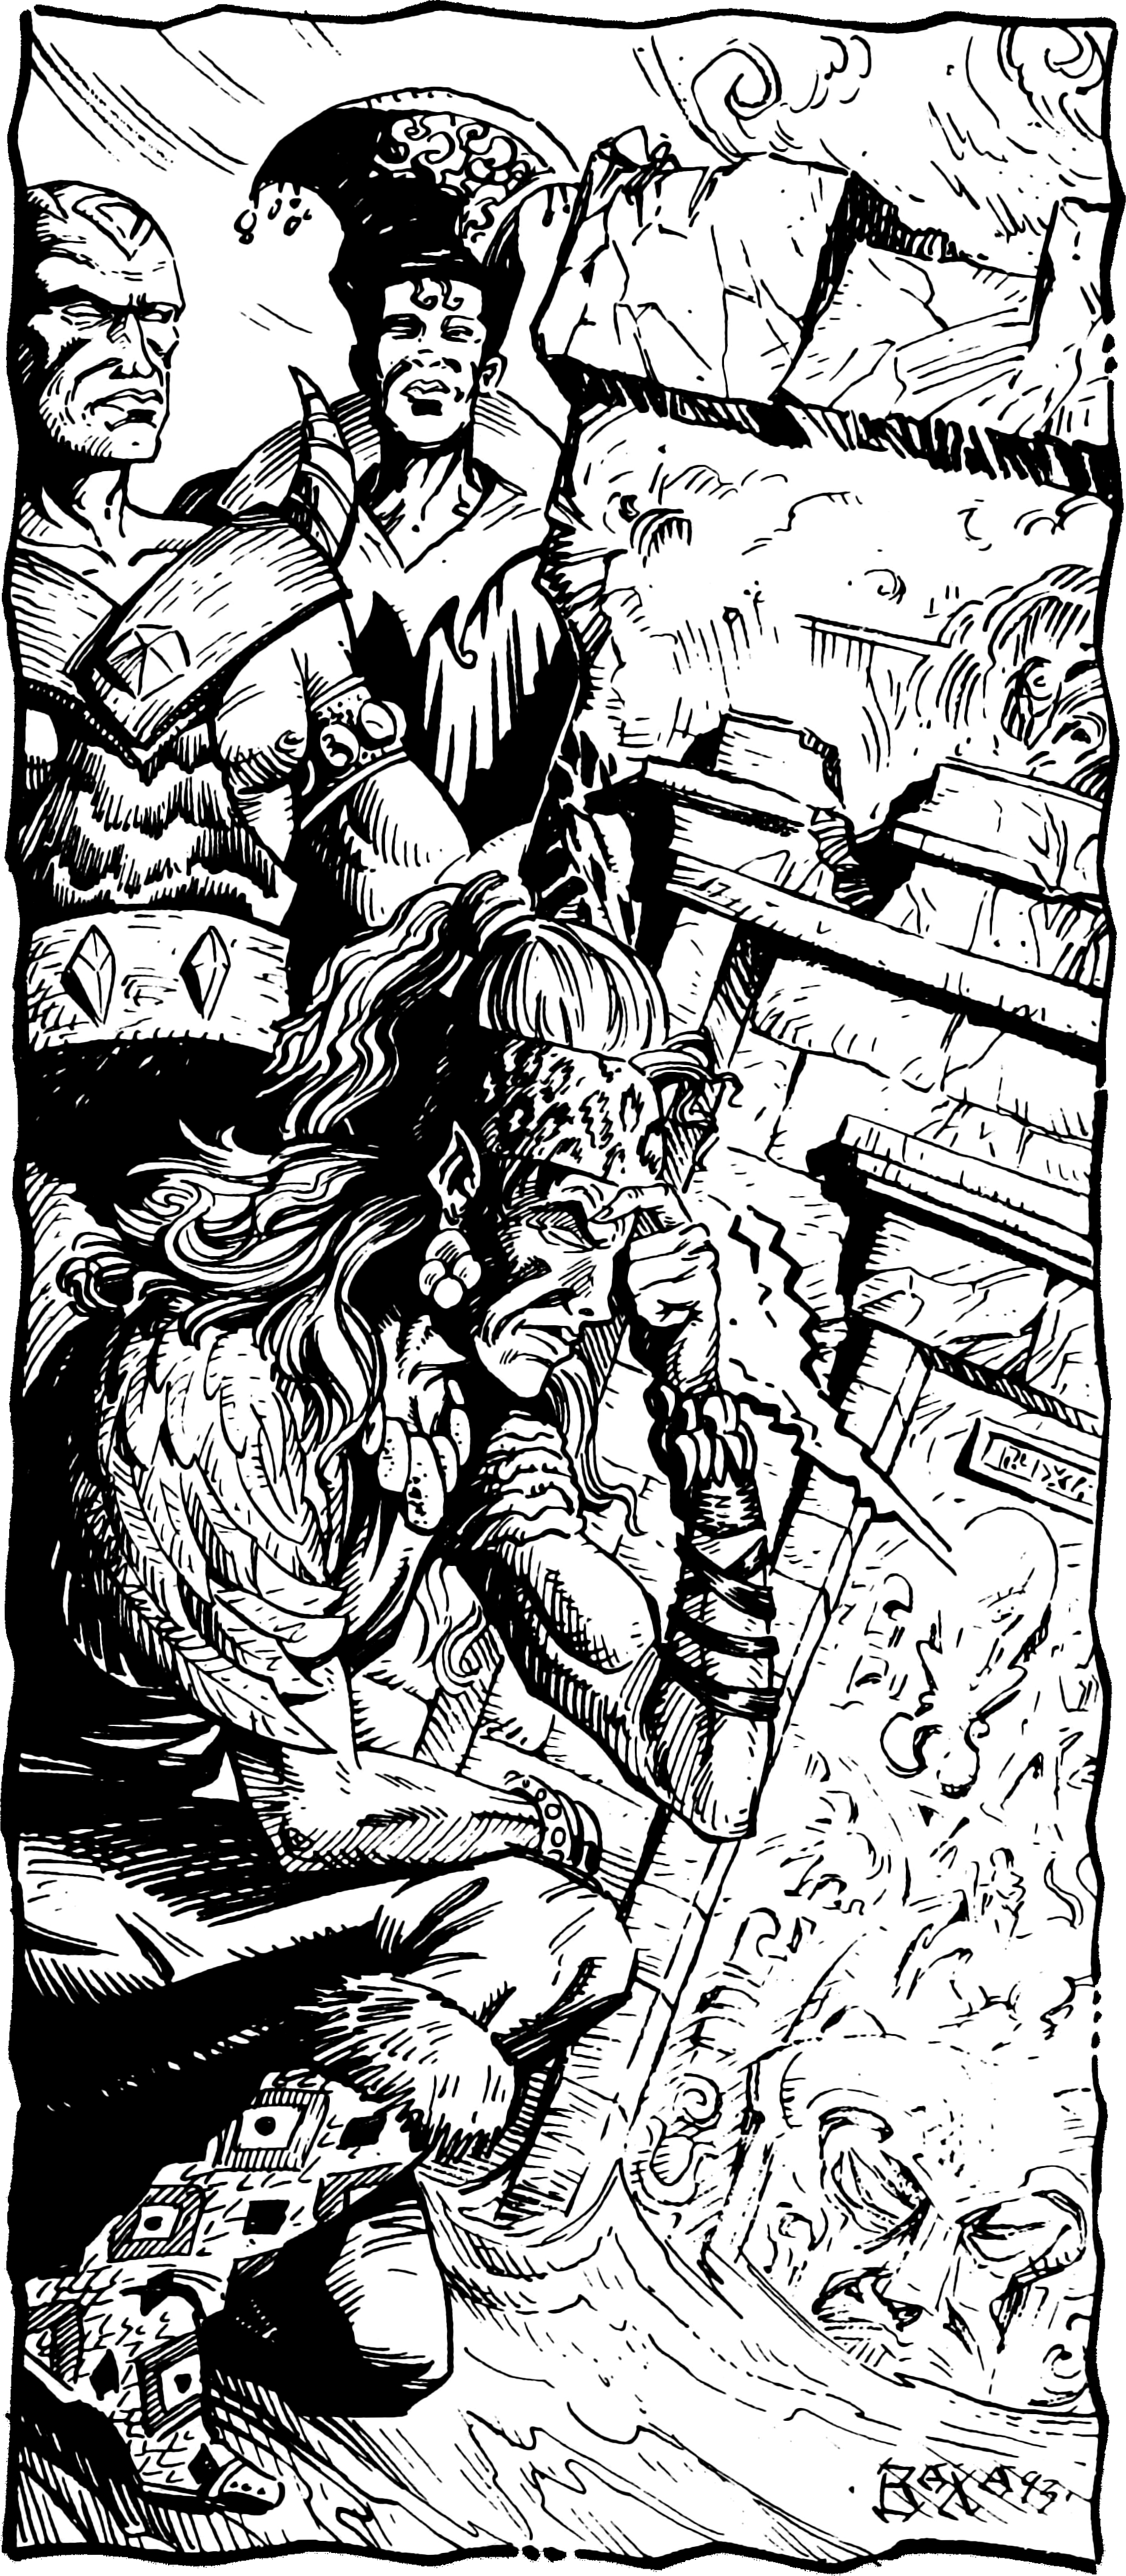
\includegraphics[width=\columnwidth-7mm]{images/cleric-4.png}
% \WOTC
% \end{figure}

\subsection{Other Sources}
In addition to the many options presented here, a few more base classes should be considered for {\tableheader Dark Sun} characters. This edition made a revision in most of the base classes. Because of this, some minor changes are suggested for each class.

\textbf{Scout} (\emph{Complete Adventurer}): Scout brings a mix of ranger and rogue that is adequate for the setting, being part of the core components of any caravan. When using this class, change the rate of bonus feats to: at 4th level and every three levels thereafter (7th, 10th, 13th, 16th, and 19th level).

\textbf{Lurk} (\emph{Complete Psionic}): This psionic rogue is as prevalent as any psychic warrior. When using this class, change the number of power points per day to match a psychic warrior of the same level.

% \begin{figure*}[b]
% \centering
% 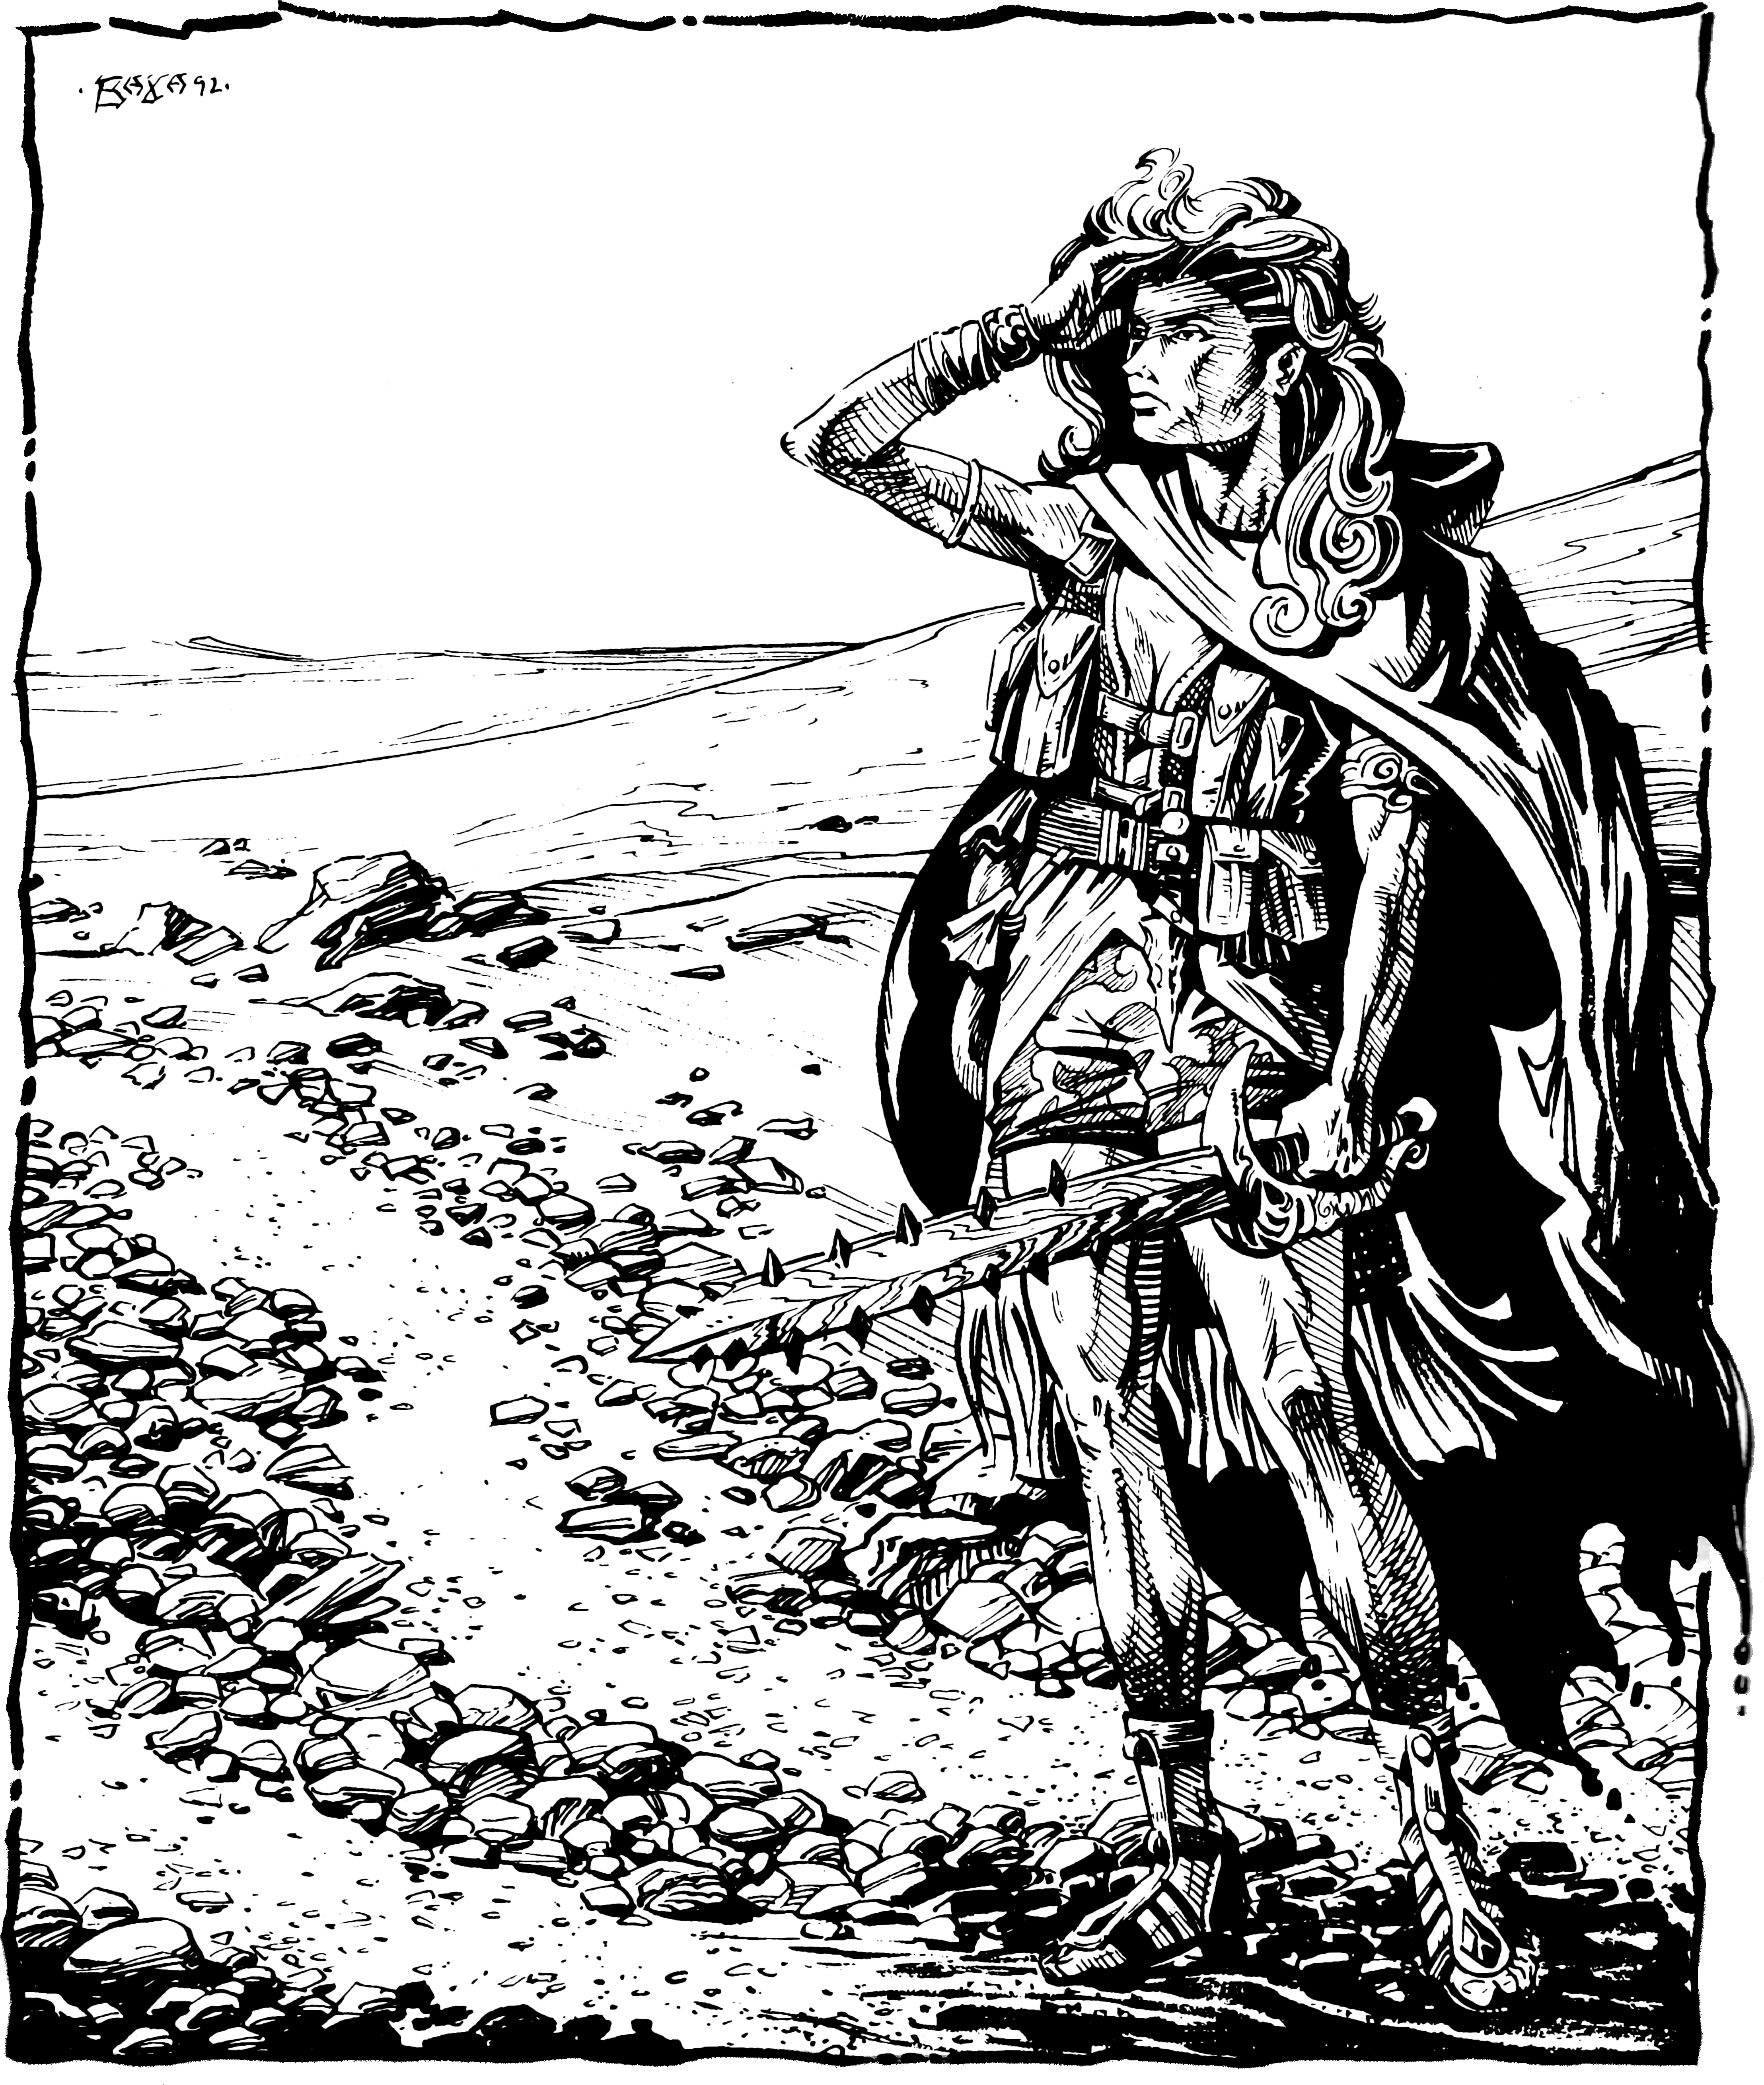
\includegraphics[width=\textwidth]{images/adventurer-1.png}
% \WOTC
% \end{figure*}

\clearpage
\Class{Barbarian}
{Gith's blood! I will hunt that wizard down and skin him alive.}{Borac, mul barbarian}

Brutality is a way of life in Athas, as much in some of the cities as in the dwindling tribes of Athas' harsh wastes. Cannibal headhunting halflings (who occasionally visit Urik from the Forest Ridge) sometimes express shock at the savagery and bloodshed of the folk that call themselves ``civilized'' and live between walls of stone. They would be more horrified if they were to see the skull piles of Draj, experience the Red Moon Hunt in Gulg, or watch a seemingly docile house slave in Eldaarich rage as she finally ``goes feral'', taking every frustration of her short cruel life out on whoever happens to be closest to hand. Nibenese sages claim that the potential for savagery is in every sentient race, and the history of Athas seems to support their claim.

Some on Athas have turned their brutality into an art of war. They are known as ``brutes'', ``barbarians'' or ``feral warriors'' and they wear the name with pride. Impious but superstitious, cunning and merciless, fearless and persistent, they have carved a name for their martial traditions out of fear and blood.

\WarriorTable{The Barbarian}{
1st  & +1             & +2  & +0 & +0 & Fast movement, rage 1/day               \\
2nd  & +2             & +3  & +0 & +0 & Uncanny dodge                           \\
3rd  & +3             & +3  & +1 & +1 & Wasteland trap sense +1                 \\
4th  & +4             & +4  & +1 & +1 & Rage 2/day                              \\
5th  & +5             & +4  & +1 & +1 & Improved uncanny dodge                  \\
6th  & +6/+1          & +5  & +2 & +2 & Wasteland trap sense +2                 \\
7th  & +7/+2          & +5  & +2 & +2 & Damage reduction 1/--                   \\
8th  & +8/+3          & +6  & +2 & +2 & Bonus feat, rage 3/day                  \\
9th  & +9/+4          & +6  & +3 & +3 & Greater rage, wasteland trap sense +3   \\
10th & +10/+5         & +7  & +3 & +3 & Damage reduction 2/--                   \\
11th & +11/+6/+1      & +7  & +3 & +3 & Bonus feat                              \\
12th & +12/+7/+2      & +8  & +4 & +4 & Rage 4/day, wasteland trap sense +4     \\
13th & +13/+8/+3      & +8  & +4 & +4 & Indomitable will, damage reduction 3/-- \\
14th & +14/+9/+4      & +9  & +4 & +4 & Bonus feat                              \\
15th & +15/+10/+5     & +9  & +5 & +5 & Tireless rage, wasteland trap sense +5  \\
16th & +16/+11/+6/+1  & +10 & +5 & +5 & Damage reduction 4/--, rage 5/day       \\
17th & +17/+12/+7/+2  & +10 & +5 & +5 & Bonus feat, mighty rage                 \\
18th & +18/+13/+8/+3  & +11 & +6 & +6 & Wasteland trap sense +6                 \\
19th & +19/+14/+9/+4  & +11 & +6 & +6 & Damage reduction 5/--                   \\
20th & +20/+15/+10/+5 & +12 & +6 & +6 & Bonus feat, rage 6/day                  \\
}

\begin{figure}[t!]
\centering
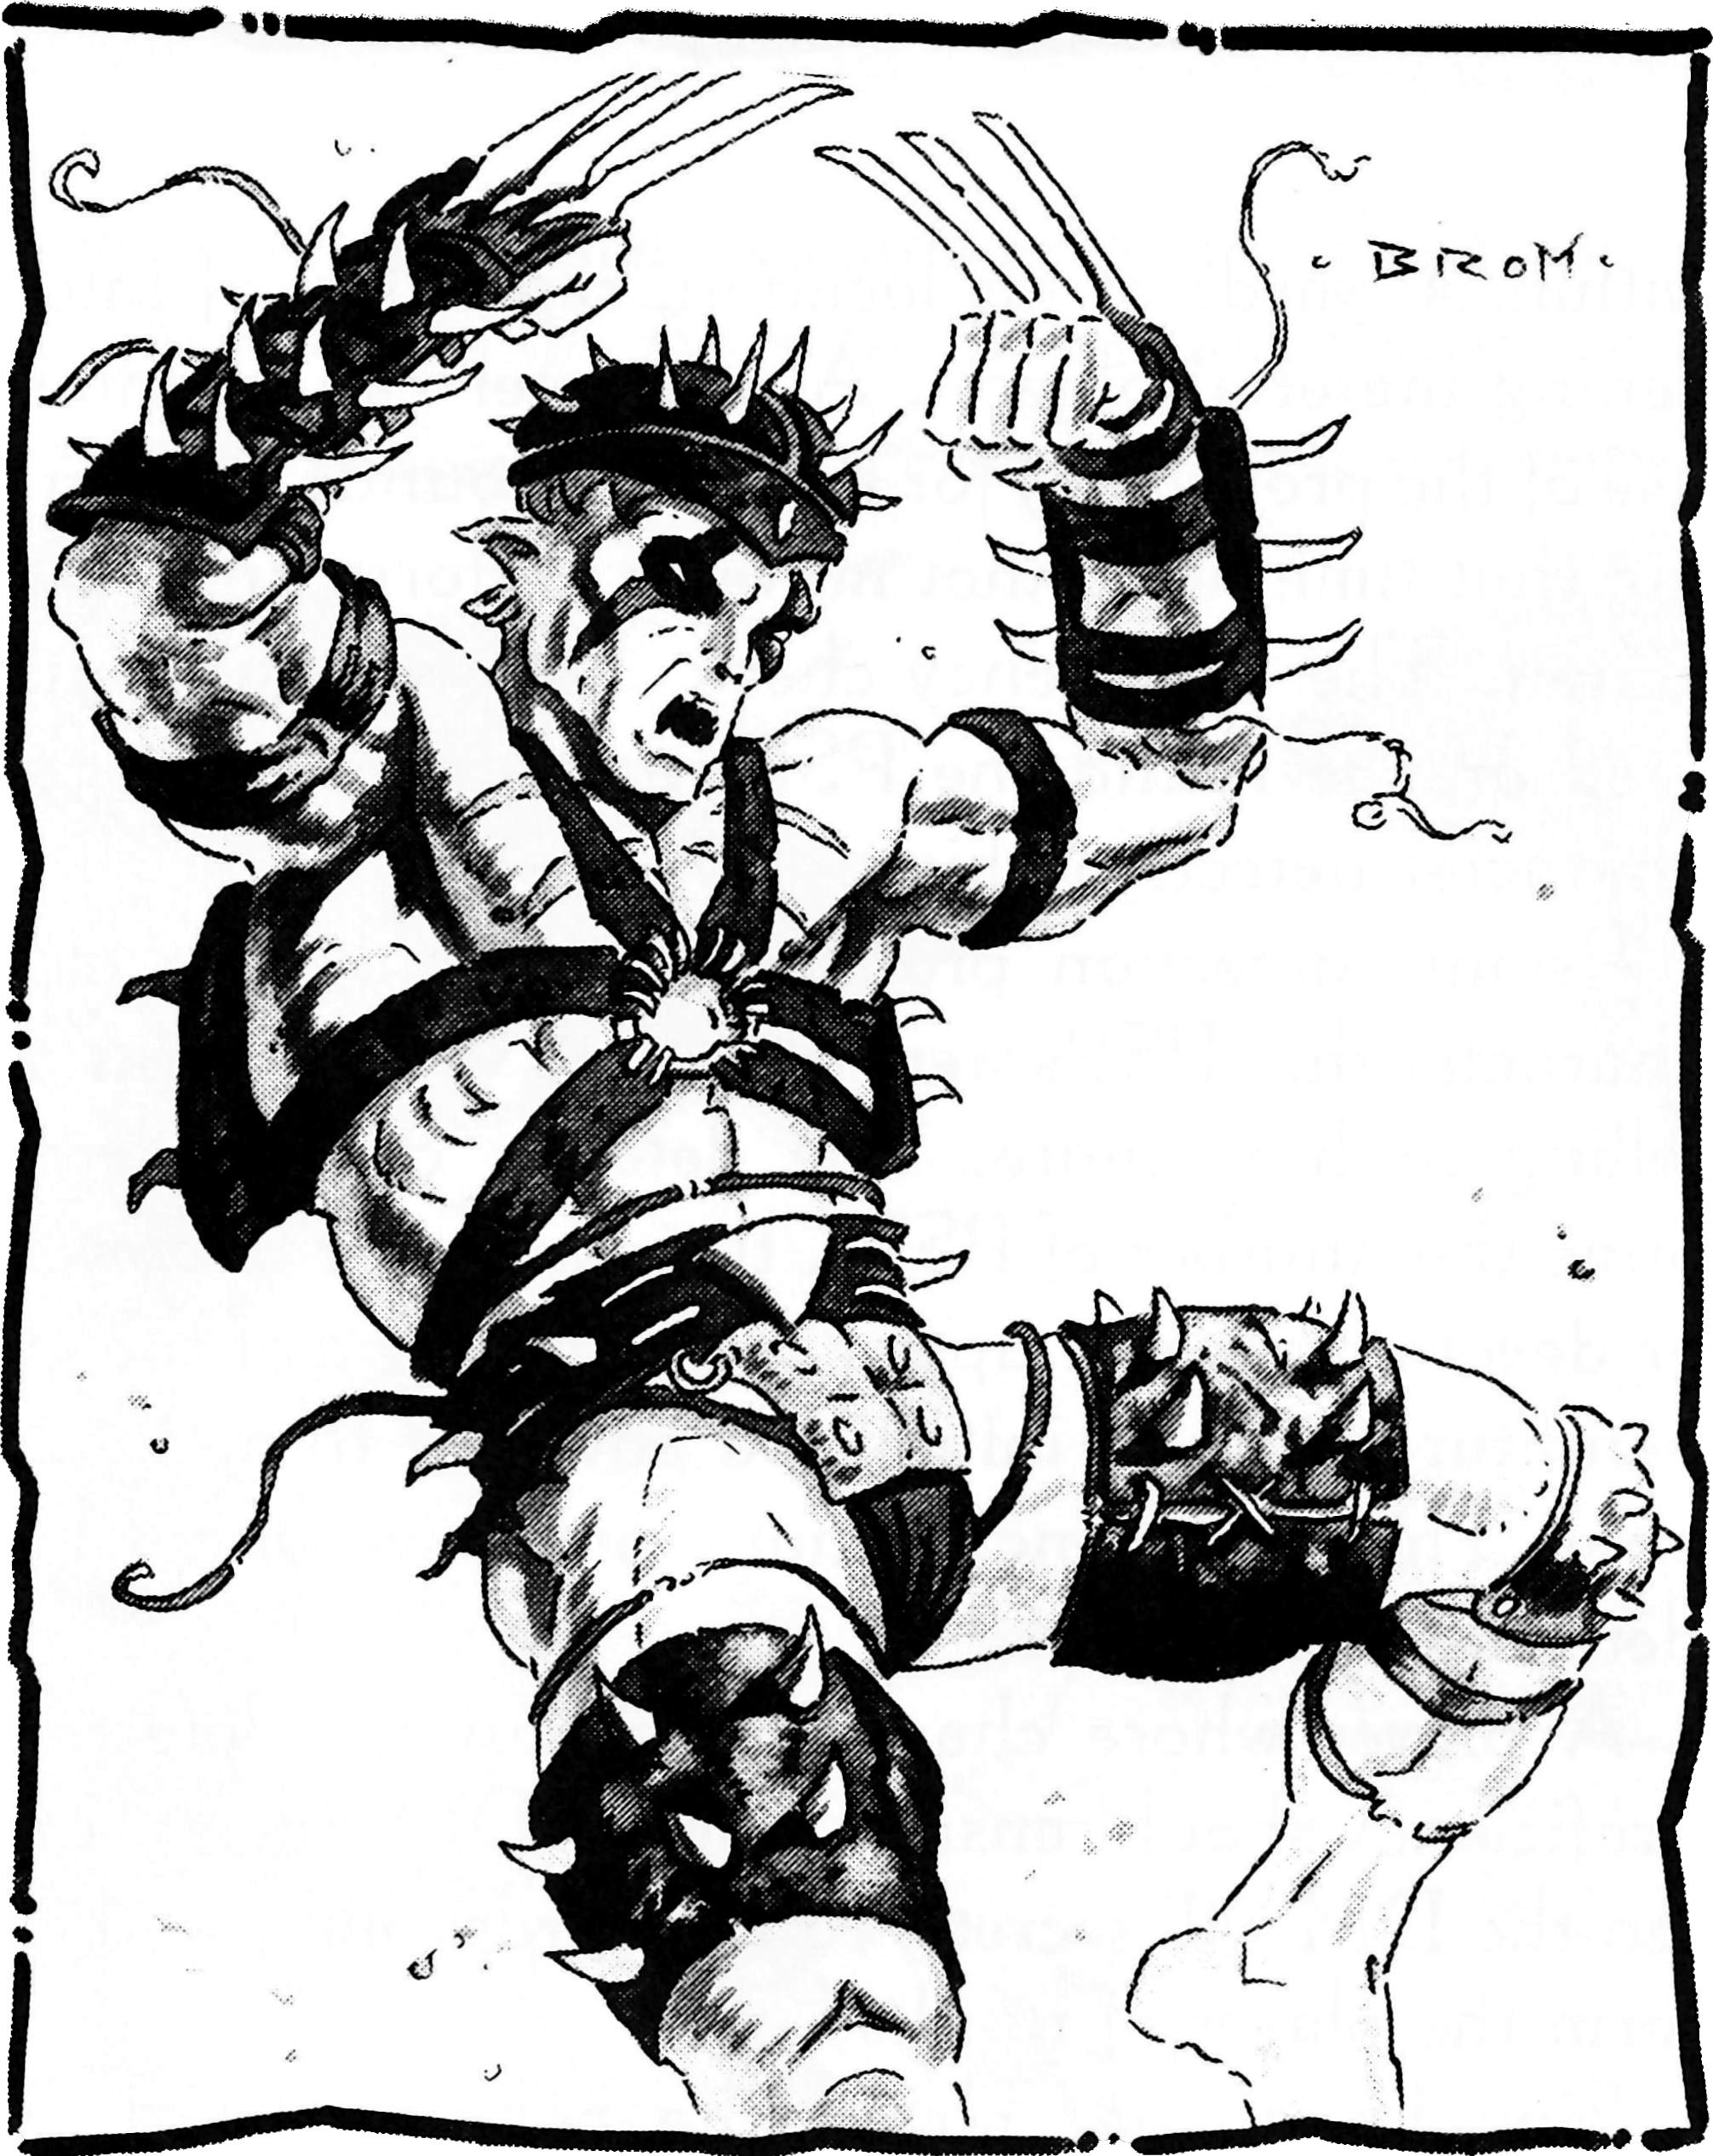
\includegraphics[width=\columnwidth]{images/barbarian-1.png}
\WOTC
\end{figure}

\subsection{Making a Barbarian}

The barbarian is a fearsome warrior, compensating for lack of training and discipline with bouts of powerful rage. While in this berserk fury, barbarians become stronger and tougher, better able to defeat their foes and withstand attacks. These rages leave barbarians winded; at first they only have the energy for a few such spectacular displays per day, but those few rages are usually sufficient.

\textbf{Races:} Humans are often barbarians, many having been raised in the wastes or escaped from slavery. Half-elves sometimes become barbarians, having been abandoned by their elven parents to the desert to survive on their own; if more of them survived they would be quite numerous. Dwarves are very rarely barbarians, but their mul half-children take to brutishness like a bird takes to flight, living by their wits and strengths in the wastes. Muls have a particular inclination this way of life, and very often ``go feral'' in the wilderness after escaping slavery in the city. Elves rarely take to the barbarian class; those that do are usually from raiding tribes such as the Silt Stalkers. Half-giants readily take the barbarian class. Despite their feral reputations, halflings rarely become barbarians; their small statures and weak strength adapts them better for the ranger class. Likewise, despite their wild nature, thri-kreen are rarely barbarians since their innate memories allow them to gain more specialized classes, such as ranger, without training. Pterrans of the Forest Ridge occasionally become barbarians, but like halflings they more often favor the ranger class.

\textbf{Alignment:} Barbarians are never lawful---their characteristic rage is anything but disciplined and controlled. Many barbarians in the cities are often rejects from the regular army, unable to bear regular discipline or training. Some may be honorable, but at heart they are wild. At best, chaotic barbarians are free and expressive. At worst, they are thoughtlessly destructive.

\subsection{Game Rule Information}
\textbf{Alignment:} Any nonlawful.

\textbf{Hit Die:} d12.

\subsubsection{Class Skills}
\skill{Autohypnosis} (Wis), \skill{Climb} (Str), \skill{Craft} (Int), \skill{Escape Artist} (Des), \skill{Handle Animal} (Cha), \skill{Intimidate} (Cha), \skill{Jump} (Str), \skill{Knowledge} (nature) (Int), \skill{Listen} (Wis), \skill{Profession} (Wis), \skill{Ride} (Dex), and \skill{Survival} (Wis).

\textbf{Skill Points per Level:} 4 + Int modifier ($\times4$ at 1st level).

\subsubsection{Class Features}

\textbf{Weapon and Armor Proficiency:} A barbarian is proficient with all simple and martial weapons, light armor, medium armor, and shields (except tower shields).

\textbf{Fast Movement (Ex):} A barbarian's land speed is faster than the norm for his race by +3 meters. This benefit applies only when he is wearing no armor, light armor, or medium armor and not carrying a heavy load. Apply this bonus before modifying the barbarian's speed because of any load carried or armor worn.

\textbf{Rage (Ex):} A barbarian can fly into a rage a certain number of times per day. In a rage, a barbarian temporarily gains a +4 bonus to Strength, a +4 bonus to Constitution, and a +2 morale bonus on Will saves, but he takes a $-2$ penalty to Armor Class. The increase in Constitution increases the barbarian's hit points by 2 points per level, but these hit points go away at the end of the rage when his Constitution  score drops back to normal. (These extra hit points are not lost first the way temporary hit points are.) While raging, a barbarian cannot use any Charisma-, Dexterity-, or Intelligence-based skills (except for \skill{Balance}, \skill{Escape Artist}, \skill{Intimidate}, and \skill{Ride}), the \skill{Concentration} skill, or any abilities that require patience or concentration, nor can he cast spells or activate magic items that require a command word, a spell trigger (such as a wand), or spell completion (such as a scroll) to function. He can use any feat he has except \feat{Combat Expertise}, item creation feats, and metamagic feats. A fit of rage lasts for a number of rounds equal to 3 + the character's (newly improved) Constitution modifier. A barbarian may prematurely end his rage. At the end of the rage, the barbarian loses the rage modifiers and restrictions and becomes fatigued ($-2$ penalty to Strength, $-2$ penalty to Dexterity, can't charge or run) for the duration of the current encounter (unless he is a 15th-level barbarian, at which point this limitation no longer applies).

A barbarian can fly into a rage only once per encounter. At 1st level he can use his rage ability once per day. At 4th level and every four levels thereafter, he can use it one additional time per day (to a maximum of six times per day at 20th level). Entering a rage takes no time itself, but a barbarian can do it only during his action, not in response to someone else's action. 

\textbf{Uncanny Dodge (Ex):} At 2nd level, a barbarian retains his Dexterity bonus to AC (if any) even if he is caught flat-footed or struck by an invisible attacker. However, he still loses his Dexterity bonus to AC if immobilized. If a barbarian already has uncanny dodge from a different class, he automatically gains improved uncanny dodge instead.

\textbf{Wasteland Trap Sense (Ex):} Starting at 3rd level, a barbarian gains a +1 bonus on Reflex saves made to avoid traps and natural hazards, and a +1 dodge bonus to AC against attacks made by traps and natural hazards. These bonuses rise by +1 every three barbarian levels thereafter (6th, 9th, 12th, 15th, and 18th level). Trap sense bonuses gained from multiple classes stack.

\textbf{Improved Uncanny Dodge (Ex):} At 5th level and higher, a barbarian can no longer be flanked. This defense denies a rogue the ability to sneak attack the barbarian by flanking him, unless the attacker has at least four more rogue levels than the target has barbarian levels. If a character already has uncanny dodge from a second class, the character automatically gains improved uncanny dodge instead, and the levels from the classes that grant uncanny dodge stack to determine the minimum level a rogue must be to flank the character.

\begin{figure}[t!]
\centering
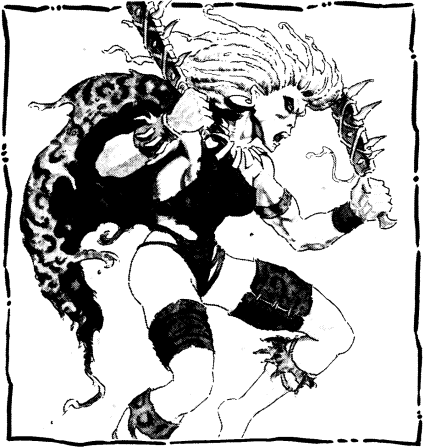
\includegraphics[width=\columnwidth]{images/halfling-1.png}
\WOTC
\end{figure}

\textbf{Damage Reduction (Ex):} At 7th level, a barbarian gains Damage Reduction. Subtract 1 from the damage the barbarian takes each time he is dealt damage from a weapon or a natural attack. At 10th level, and every three barbarian levels thereafter (13th, 16th, and 19th level), this damage reduction rises by 1 point. Damage reduction can reduce damage to 0 but not below 0.

\textbf{Bonus Feat:} At 8th level and every three levels thereafter (11th, 14th, 17th, and 20th level), a barbarian gains a bonus feat, which must be selected from the following list:
\feat{Awesome Blow},
\feat{Blind-Fight},
\feat{Cleave},
\feat{Closed Mind},
% \feat{Combat Reflexes},
Dash\textsuperscript{CW},
Destructive Rage\textsuperscript{CW},
\feat{Diehard},
\feat{Endurance},
Extend Rage\textsuperscript{CW},
Extra Rage\textsuperscript{CW},
% Faster Healing\textsuperscript{CW},
Fleet of Foot\textsuperscript{CW},
\feat{Great Cleave},
% \feat{Greater Critical},
Greater Resiliency\textsuperscript{CW},
\feat{Hard as Rock},
\feat{Hostile Mind},
\feat{Improved Bull Rush},
% \feat{Improved Critical},
% \feat{Improved Initiative},
\feat{Improved Sunder},
\feat{Innate Hunter},
Instantaneous Rage\textsuperscript{CW},
Intimidating Rage\textsuperscript{CW},
\feat{Mind Over Body},
\feat{Power Attack},
% \feat{Psionic Hole},
% \feat{Quick Draw},
\feat{Rapid Metabolism},
\feat{Reckless Offense},
\feat{Run},
Steadfast Determination\textsuperscript{PH2},
\feat{Toughness},
\feat{Track},
\feat{Wastelander}.
He must meet all the prerequisites for the feat.

\textbf{Greater Rage (Ex):} At 8th level, a barbarian's bonuses to Strength and Constitution during his rage each increase to +6, and his morale bonus on Will saves increases to +3. The penalty to AC remains at $-2$.

\textbf{Indomitable Will (Ex):} While in a rage, a barbarian of 13th level or higher gains a +4 bonus on Will saves to resist enchantment spells and telepathy powers. This bonus stacks with all other modifiers, including the morale bonus on Will saves he also receives during his rage.

\textbf{Tireless Rage (Ex):} At 15th level and higher, a barbarian no longer becomes fatigued at the end of his rage.

\textbf{Mighty Rage (Ex):} At 17th level, a barbarian's bonuses to Strength and Constitution during his rage each increase to +8, and his morale bonus on Will saves increases to +4. The penalty to AC remains at $-2$.

\subsubsection{Ex-Barbarians}
A barbarian who becomes lawful loses the ability to rage and cannot gain more levels as a barbarian. He retains all the other benefits of the class (damage reduction, fast movement, wasteland trap sense, and uncanny dodge).


\subsection{Playing a Barbarian}
All cower and stand in awe at the fury you can tap, enhancing your strength and toughness. But what do these people know of the burnt wastes of Athas, the hellish jungles of the Forest Ridge? The cruel vicissitudes of growing up in the wastes of Athas were nothing but normal to you. When your family was lost in a tembo attack, or when your entire village was either murdered or forced into slavery, how could you not know they might not had to die? These and many other brutal experiences marked you, and you now stand apart from those born into the ``comforts'' of the city-states.

\subsubsection{Religion}
Although most are profoundly superstitious, barbarians distrust the established elemental temples of the cities. Some worship the elements of fire or air or devote themselves to a famous figure. Most barbarians truly believe the sorcerer-kings to be gods, because of their undeniable power, and a few actually worship a sorcerer-king, usually the one that conquered their tribe. Such barbarians often escape menial slavery by joining an elite unit of barbarians in the service of an aggressive city-state such as Urik, Draj or Gulg.

\subsubsection{Other Classes}
Barbarians are most comfortable in the company of gladiators, and of clerics of Air and Fire. Enthusiastic lovers of music and dance, barbarians admire bardic talent, and some barbarians also express fascination with bardic poisons, antidotes and alchemical concoctions. With some justification, barbarians do not trust wizardry. Even though many barbarians manifest a wild talent, they tend to be wary of psions and Tarandan psionicists. Psychic warriors, on the other hand, are creatures after the barbarian's own heart, loving battle for its own sake. Barbarians have no special attitudes toward fighters or rogues. Barbarians admire gladiators and will ask about their tattoos and exploits, but will quickly grow bored if the gladiator does not respond boastfully.

\subsubsection{Combat}
You know that half the battle occurs before the fight even begins. You prefer to choose your battleground when you can, stalking your opponent into terrain that best suits your abilities. Once battle is joined, you become a wild frenzy of motion, striking quickly and powerfully until all your opponents are crushed. While you lack the training of the fighter, or the cunning of the gladiator, you more than compensate them through sheer power and resilience.

\subsubsection{Advancement}
Becoming a barbarian let you further tap into your feral nature, letting you become one with the savage beast in your hear, and through your training, you have learned what you must do to unlock it.

To fully utilize your barbarian abilities, you will want to focus on feats that take advantage of your superior strength and speed, such as Power Attack and Whirlwind Attack.


\subsection{Starting Packages}
\subsubsection{The Survivor}
Human Barbarian

\textbf{Ability Scores:} Str 15, Dex 13, Con 14, Int 10, Wis 12, Cha 8.

\textbf{Skills:} \skill{Climb}, \skill{Escape Artist}, \skill{Listen}, \skill{Survival}.

\textbf{Languages:} Common.

\textbf{Feat:} \feat{Great Fortitude}, \feat{Wastelander}.

\textbf{Weapons:} Carrikal (1d8/$\times$3)

Atlatl with 10 javelins (1d6/$\times$3, 12 m).

\textbf{Armor:} Scale mail (+4 AC).

\textbf{Gear:} Standard adventurer's kit, 13 cp.

\subsubsection{The Crusher}
Half-giant Barbarian

\textbf{Ability Scores:} Str 23, Dex 10, Con 18, Int 6, Wis 9, Cha 4.

\textbf{Skills:} \skill{Climb}, \skill{Intimidate}, \skill{Jump}.

\textbf{Languages:} Common.

\textbf{Feat:} \feat{Exotic Weapon Proficiency} (swatter).

\textbf{Weapons:} Swatter (3d8/$\times$4).

\textbf{Armor:} Leather (+2 AC).

\textbf{Gear:} Standard adventurer's kit, 0 cp.

\subsubsection{The Hunter}
Thri-kreen Barbarian

\textbf{Ability Scores:} Str 15, Dex 14, Con 12, Int 10, Wis 13, Cha 8.

\textbf{Skills:} \skill{Jump}, \skill{Knowledge} (nature), \skill{Search}, \skill{Survival}.

\textbf{Languages:} Kreen.

\textbf{Feat:} \feat{Track}.

\textbf{Weapons:} Four chatkchas (1d6, 6 m).

\textbf{Armor:} Heavy wooden shield (+2 AC).

\textbf{Gear:} Standard adventurer's kit, 13 cp.


\subsection{Barbarians on Athas}
\Quote{Don't make my friend angry. You won't like him when he's angry.}{Cabal, half-elven bard}

In a savage world like Athas, is only natural that some of its inhabitants have turned into barbarians. They are fierce combatants without the army training fighters receive or wild rangers without the hunting skills.

\subsubsection{Daily Life}
A barbarian is a passionate adventurer. As a survivalist, he often sees his involvement in a particular enterprise as a validation of his superior strength and resilience. In his mind, his presence alone is enough to ensure the success of a quest, adventure, or ruin raid. Even simple tasks are additional opportunities to prove his own worth by accomplishing the task with might and alacrity. Barbarians are typically hardheaded and unforgiving because of the rigors of his previous life.

\subsubsection{Notables}
It is rare for a barbarian to live long enough, or close enough to civilization, in order to become famous, but a few examples exist. Korno, a Raamite gladiator, became the leader of a group of slaves, and Korno's furious rage known from the arenas has only increased after losing everything in the Raam invasion by Dregoth. The leader of Pillage, Chilod, is a tarek know for his outbursts of rage and cruelty, being one of the most feared chiefs of the Bandit States.

\subsubsection{Organizations}
Because of their independent and sometimes downright chaotic natures, many barbarians refuse to join organizations of any kind, though they usually maintain relationships with trading houses and raiding tribes. There is no specific organization that binds barbarians together.

\subsubsection{NPC Reactions}
Many lay people cannot tell a barbarian from a ranger or a fighter until his rage overcomes him and he starts screaming and bashing. Most authority figures and templars do not appreciate barbarians since they are prone to losing control and cannot be truly trusted. Thus, they generally treat barbarians with a great deal of caution.

\subsubsection{Barbarian Lore}
Characters with ranks in \skill{Knowledge} (nature) can research barbarians to learn more about them. When a character makes a skill check, read or paraphrase the following, including the information from lower DCs.

\textbf{DC 10:} Barbarians are hot-blooded combatants who fight with great brutality and savagery.

\textbf{DC 15:} Barbarians become stronger and more resilient when they lose control.

\textbf{DC 20:} Barbarians can stand up to punishment that no other individual can endure, and their reflexes are as quick as a rogue's.
\Class{Bard}
{Some people think a club can solve any problem. Unless you're a half-giant, there are more sophisticated ways of settling a disagreement.}{Cabal, half-elven bard}

From the shadowy corners of Athas' most disreputable places hails the bard. Like their counterparts in other fantasy worlds, Athasian bards are the unquestioned masters of oral tradition and forgotten lore, but rather than sharing their lore with whoever will listen, Athasian bards guard their secrets as jealously as the sorcerer-kings harbor their water and iron. Athasian bards may sell information to the highest bidder; they peddle their services and the fruits of their knowledge, but trade secrets are what give bards an edge on the uninitiated. Bards would rather die than reveal these secrets.

Meeting a bard can be an uneasy encounter, since one never knows how the bard has chosen to devote his multiple talents. Some bards master the art of making poisons, and survive by selling these poisons and their antidotes for those who have coin to pay. Some bards master the art of entertainment, using their performances to amuse nobles and templars and gain wealth. Some become assassins, mixing their knowledge of poison and stealth to become hired hands. Bards' unique position in the Athasian society means they often overhear conversations between high-ranking templars or nobles, or they may have treated an injured person that prefers to remain anonymous. Respectable folk despise them; the powerful fear them; but in the Athasian cities, everyone eventually comes to need their services.

\WarriorTable[b{0.8cm} b{2.6cm} Z{1.4cm} Z{1.4cm} Z{1.4cm} X]{The Bard}{
1st  & +0         & +2  & +2  & +2  & Bardic music, bardic knowledge, smuggler, countersong, \emph{fascinate}, inspire courage +1\\
2nd  & +1         & +3  & +3  & +3  & Poison use, streetsmart                                  \\
3rd  & +2         & +3  & +3  & +3  & Inspire competence, \feat{Quick Draw}                    \\
4th  & +3         & +4  & +4  & +4  & Trade secret                                             \\
5th  & +3         & +4  & +4  & +4  & Mental resistance                                        \\
6th  & +4         & +5  & +5  & +5  & Improved poison use, \emph{suggestion}, quick thinking +2\\
7th  & +5         & +5  & +5  & +5  & Chance 1/day, inspire courage +2                         \\
8th  & +6/+1      & +6  & +6  & +6  & Trade secret                                             \\
9th  & +6/+1      & +6  & +6  & +6  & Inspire greatness, speed reactions                       \\
10th & +7/+2      & +7  & +7  & +7  & Special ability                                          \\
11th & +8/+3      & +7  & +7  & +7  & Quick thinking +4                                        \\
12th & +9/+4      & +8  & +8  & +8  & \emph{Song of freedom}, trade secret                     \\
13th & +9/+4      & +8  & +8  & +8  & Inspire courage +3                                       \\
14th & +10/+5     & +9  & +9  & +9  & Chance 2/day                                             \\
15th & +11/+6/+1  & +9  & +9  & +9  & Inspire heroics, special ability                         \\
16th & +12/+7/+2  & +10 & +10 & +10 & Quick thinking +6, trade secret                          \\
17th & +12/+7/+2  & +10 & +10 & +10 & Awareness                                                \\
18th & +13/+8/+3  & +11 & +11 & +11 & \emph{Mass suggestion}, \emph{mind blank}                \\
19th & +14/+9/+4  & +11 & +11 & +11 & Inspire courage +4                                       \\
20th & +15/+10/+5 & +12 & +12 & +12 & Special ability, trade secret                            \\
}

\Figure*{t}{images/bard-2.png}

\subsection{Making a Bard}
Bards receive numerous abilities they can use to survive. Many become masters of poisons, selling their illegal substances to anyone. Alone of the classes, bards hold the secrets of alchemy, creating fiery concoctions and mysterious mixes. Bards are master smugglers, selling spell components and other illegal items in the Bard's Quarters of the city-states. All bards, however, have some degree of entertainment skill. The songs of most bards can dazzle a crowd, or incite them to riot. Bards tend to learn to play a variety of instruments, or recite poetry or old legends by campfire. They can be acrobats, performing dazzling displays of physical prowess. They are often called upon as sources of information.

\textbf{Abilities:} Charisma is the most important ability for a bard, because many of their abilities and skills are affected by it. A high Dexterity improves the bard's defensive ability. Intelligence is also important because it bolster the numbers of skills he has access.

\textbf{Races:} All humanoid races of Athas can become bards. The social stigma in certain regions may be higher than others, however. For example, the loremasters of the halflings of the Jagged Cliffs are highly regarded because of the ancient secrets and histories they preserve. But in the city-states, where the Bard's Quarters are notorious, being a bard is not usually a good thing. Elven tribes often have a bard, who keeps the history of the tribe alive, its conquests and defeats. Humans are often bards, becoming performers of great talent, or assassins of deadly skill and precision. Half-elves, because of their lonely existence, often take to being bards. The prejudice they face at every stage in life can move some to become great poets or singers. Muls and half-giants make poor bards; their talents are usually better served elsewhere than the stage or the shadows of alleys. As well, thri-kreen are rarely seen as bards, relying instead upon their racial memory.

\textbf{Alignment:} Most bards are chaotic, and operate alone, brokering information, arranging deals, smuggling illegal wares such as poisons, drugs, spell components and other things. Neutral bards are the ones most likely to operate in fellowships with adventurers, or entertain in troupes with other bards. The rare lawful bards can easily secure positions as councilors or agents for templars, and noble and merchant houses. Good bards are often entertainers or lorekeepers, putting their talents to benevolent use, sometimes diagnosing poisonings and selling the proper antidotes. Evil bards are often masters of poisons and alchemy, selling their wares to anyone with the ceramic to pay.

\subsection{Game Rule Information}

\textbf{Hit Die:} d6.

\subsubsection{Class Skills}
\skill{Appraise} (Int), \skill{Balance} (Dex), \skill{Bluff} (Cha), \skill{Climb} (Str), \skill{Craft} (Int), \skill{Decipher Script} (Int), \skill{Diplomacy} (Cha), \skill{Disguise} (Cha), \skill{Escape Artist} (Dex), \skill{Forgery} (Int), \skill{Gather Information} (Cha), \skill{Heal} (Wis), \skill{Hide} (Dex), \skill{Intimidate} (Cha), \skill{Jump} (Str), \skill{Knowledge} (all skills individually) (Int), \skill{Listen} (Wis), \skill{Move Silently} (Dex), \skill{Perform} (Cha), \skill{Profession} (Wis), \skill{Ride} (Dex), \skill{Search} (Int), \skill{Sense Motive} (Wis), \skill{Sleight of Hand} (Dex), \skill{Speak Language} (N/A), \skill{Tumble} (Dex), \skill{Use Magic Device} (Cha), \skill{Use Psionic Device} (Cha), and \skill{Use Rope} (Dex).

\textbf{Skill Points per Level:} 6 + Int modifier ($\times4$ at 1st level).

\subsubsection{Class Features}

\textbf{Weapon and Armor Proficiency:} You are proficient in all simple weapons, plus the bard's friend, all crossbows, garrote, greater blowgun, whip and widow's knife. You are proficient in light armor, but not shields.

\textbf{Bardic Knowledge:} A bard may make a special bardic knowledge check with a bonus equal to his bard level + his Intelligence modifier to see whether he knows some relevant information about local notable people, legendary items, or noteworthy places. (If the bard has 5 or more ranks in \skill{Knowledge} (history), he gains a +2 bonus on this check.)

A successful bardic knowledge check will not reveal the powers of a magic item but may give a hint as to its general function. A bard may not take 10 or take 20 on this check; this sort of knowledge is essentially random.

\Table{}{p{0.6cm} X}{
\tableheader DC & \tableheader Type of Knowledge\\
10 & Common, known by at least a substantial minority of the local population.\\
20 & Uncommon but available, known by only a few people legends.\\
25 & Obscure, known by few, hard to come by.\\
30 & Extremely obscure, known by very few, possibly forgotten by most who once knew it, possibly known only by those who don't understand the significance of the knowledge.}

\textbf{Bardic Music:} Once per day per bard level, a bard can use his song or poetics to produce magical effects on those around him (usually including himself, if desired). While these abilities fall under the category of bardic music and the descriptions discuss singing or playing instruments, they can all be activated by reciting poetry, chanting, singing lyrical songs, singing melodies, whistling, playing an instrument, or playing an instrument in combination with some spoken performance. Each ability requires both a minimum bard level and a minimum number of ranks in the \skill{Perform} skill to qualify; if a bard does not have the required number of ranks in at least one \skill{Perform} skill, he does not gain the bardic music ability until he acquires the needed ranks. A bard cannot use \skill{Perform} (arena fighting) to use his bardic music abilities.

Starting a bardic music effect is a standard action. Some bardic music abilities require concentration, which means the bard must take a standard action each round to maintain the ability. Even while using bardic music that doesn't require concentration, a bard cannot cast spells, activate magic items by spell completion (such as scrolls), spell trigger (such as wands), or command word. Just as for casting a spell with a verbal component, a deaf bard has a 20\% chance to fail when attempting to use bardic music. If he fails, the attempt still counts against his daily limit.

\textit{Countersong (Su):} A bard with 3 or more ranks in a \skill{Perform} skill can use his music or poetics to counter magical effects that depend on sound (but not spells that simply have verbal components). Each round of the countersong, he makes a \skill{Perform} check. Any creature within 9 meters of the bard (including the bard himself) that is affected by a sonic or language-dependent magical attack may use the bard's \skill{Perform} check result in place of its saving throw if, after the saving throw is rolled, the \skill{Perform} check result proves to be higher. If a creature within range of the countersong is already under the effect of a noninstantaneous sonic or language-dependent magical attack, it gains another saving throw against the effect each round it hears the countersong, but it must use the bard's \skill{Perform} check result for the save. Countersong has no effect against effects that don't allow saves. The bard may keep up the countersong for 10 rounds.

\textit{Fascinate (Sp):} A bard with 3 or more ranks in a \skill{Perform} skill can use his music or poetics to cause one or more creatures to become fascinated with him. Each creature to be fascinated must be within 27 meters, able to see and hear the bard, and able to pay attention to him. The bard must also be able to see the creature. The distraction of a nearby combat or other dangers prevents the ability from working. For every three levels a bard attains beyond 1st, he can target one additional creature with a single use of this ability.

To use the ability, a bard makes a \skill{Perform} check. His check result is the DC for each affected creature's Will save against the effect. If a creature's saving throw succeeds, the bard cannot attempt to fascinate that creature again for 24 hours. If its saving throw fails, the creature sits quietly and listens to the song, taking no other actions, for as long as the bard continues to play and concentrate (up to a maximum of 1 round per bard level). While fascinated, a target takes a $-4$ penalty on skill checks made as reactions, such as \skill{Listen} and \skill{Spot} checks. Any potential threat requires the bard to make another \skill{Perform} check and allows the creature a new saving throw against a DC equal to the new \skill{Perform} check result.

Any obvious threat, such as someone drawing a weapon, casting a spell, or aiming a ranged weapon at the target, automatically breaks the effect. Fascinate is an enchantment (compulsion), mind-affecting ability.

\textit{Inspire Courage (Su):} A bard with 3 or more ranks in a \skill{Perform} skill can use song or poetics to inspire courage in his allies (including himself), bolstering them against fear and improving their combat abilities. To be affected, an ally must be able to hear the bard sing. The effect lasts for as long as the ally hears the bard sing and for 5 rounds thereafter. An affected ally receives a +1 morale bonus on saving throws against charm and fear effects and a +1 morale bonus on attack and weapon damage rolls. At 7th level, and every six bard levels thereafter, this bonus increases by 1 (+2 at 7th, +3 at 13th, and +4 at 19th). Inspire courage is a mind-affecting ability.

\textit{Inspire Competence (Su):} A bard of 3rd level or higher with 6 or more ranks in a \skill{Perform} skill can use his music or poetics to help an ally succeed at a task. The ally must be within 9 meters and able to see and hear the bard. The bard must also be able to see the ally.

The ally gets a +2 competence bonus on skill checks with a particular skill as long as he or she continues to hear the bard's music. Certain uses of this ability are infeasible. The effect lasts as long as the bard concentrates, up to a maximum of 2 minutes. A bard can't inspire competence in himself. Inspire competence is a mind-affecting ability.

\textit{Suggestion (Sp):} A bard of 6th level or higher with 9 or more ranks in a \skill{Perform} skill can make a \spell{suggestion} (as the spell) to a creature that he has already fascinated. Using this ability does not break the bard's concentration on the fascinate effect, nor does it allow a second saving throw against the fascinate effect.

Making a \emph{suggestion} doesn't count against a bard's daily limit on bardic music \skill{perform}ances. A Will saving throw (DC 10 + \onehalf bard's level + bard's Cha modifier) negates the effect. This ability affects only a single creature (but see \emph{mass suggestion}, below). \emph{Suggestion} is an enchantment (compulsion), mind-affecting, language dependent ability.

\textit{Inspire Greatness (Su):} A bard of 9th level or higher with 12 or more ranks in a \skill{Perform} skill can use music or poetics to inspire greatness in himself or a single willing ally within 9 meters, granting him or her extra fighting capability. For every three levels a bard attains beyond 9th, he can target one additional ally with a single use of this ability (two at 12th level, three at 15th, four at 18th). To inspire greatness, a bard must sing and an ally must hear him sing. The effect lasts for as long as the ally hears the bard sing and for 5 rounds thereafter. A creature inspired with greatness gains 2 bonus Hit Dice (d10s), the commensurate number of temporary hit points (apply the target's Constitution modifier, if any, to these bonus Hit Dice), a +2 competence bonus on attack rolls, and a +1 competence bonus on Fortitude saves. The bonus Hit Dice count as regular Hit Dice for determining the effect of spells that are Hit Dice dependent. Inspire greatness is a mind-affecting ability.

\textit{Song of Freedom (Sp):} A bard of 12th level or higher with 15 or more ranks in a \skill{Perform} skill can use music or poetics to create an effect equivalent to the \spell{break enchantment} spell (caster level equals the character's bard level). Using this ability requires 1 minute of uninterrupted concentration and music, and it functions on a single target within 9 meters. A bard can't use song of freedom on himself.

\Figure{t}{images/bard-1.png}

\textit{Inspire Heroics (Su):} A bard of 15th level or higher with 18 or more ranks in a \skill{Perform} skill can use music or poetics to inspire tremendous heroism in himself or a single willing ally within 9 meters. For every three bard levels the character attains beyond 15th, he can inspire heroics in one additional creature. To inspire heroics, a bard must sing and an ally must hear the bard sing for a full round. A creature so inspired gains a +4 morale bonus on saving throws and a +4 dodge bonus to AC. The effect lasts for as long as the ally hears the bard sing and for up to 5 rounds thereafter. Inspire heroics is a mind-affecting ability.

\textit{Mass Suggestion (Sp):} This ability functions like \emph{suggestion}, above, except that a bard of 18th level or higher with 21 or more ranks in a \skill{Perform} skill can make the suggestion simultaneously to any number of creatures that he has already fascinated. \emph{Mass suggestion} is an enchantment (compulsion), mind-affecting, language-dependent ability.

\textbf{Smuggler (Ex):} A bard receives a +1 insight bonus to \skill{Bluff} and \skill{Sleight of Hand} checks for every two bard levels.

\textbf{Poison Use:} Bards are trained in the use of poisons, and as of 2nd level, never risk accidentally poisoning themselves when applying poison to a blade.

\textbf{Streetsmart (Ex):} When a bard reaches 2nd level, he gets a +2 competence bonus to \skill{Gather Information} and \skill{Intimidate} checks.

\textbf{Quick Draw:} Bards learn to strike quickly and without warning. At 3rd level, a bard gains \feat{Quick Draw} as a bonus feat.

\textbf{Trade Secrets:} At 4th level and every four levels thereafter (8th, 12th, 16th, and 20th level), a bard learns a trade secret chosen from the list below.

\textit{Alchemy Dealer (Ex):} A bard with this trade secret pays \onehalf of the market price for raw materials needed to craft alchemical items.

\textit{Coolheaded:} A bard with this trade secret may take 10 on \skill{Bluff} and \skill{Diplomacy} checks. A bard must be at least 12th level to select this trade secret.

\textit{Improvised Materials (Ex):} A bard with this trade secret can craft poisons from raw materials at hand instead of relying on specific ingredients. Doing so increases the \skill{Craft} (poisonmaking) check DC by 5 but otherwise has no effect on the poison's potency.

\textit{Poison Dealer (Ex):} A bard with this trade secret pays \onehalf of the market price for raw materials needed to craft poisons.

\textit{Poisonbane (Ex):} A bard with this trade secret receives a +4 insight bonus to \skill{Craft} (alchemy) checks when creating antitoxin and poison antidotes.

\textit{Poison Resistance (Ex):} A bard with this trade secret receives a +4 bonus to saving throws against poisons.

\textit{Scorpion's Touch:} A bard with this trade secret adds +1 to the save DC of all poisons applied by him. This trade secret may be chosen more than once, and its effects stack.

\textit{Skilled:} A bard with this trade secret adds \onequarter your bard level as a competence bonus to one of the following skills: \skill{Appraise}, \skill{Bluff}, \skill{Craft}, \skill{Diplomacy}, \skill{Heal}, \skill{Perform}, \skill{Profession}, \skill{Sense Motive} or \skill{Sleight of Hand}. This trade secret may be chosen more than once, each time it applies to a different skill.

\textit{Smokestick Application (Ex):} A bard with this trade secret can combine inhaled poisons with smokesticks. All creatures within the area the smokestick covers (3-m cube) are affected by the poison you applied to the smokestick.

\textit{Versatile:} A bard with this trade secret selects any two non-class skills to be considered class skills.


\textbf{Mental Resistance (Ex):} Bards carry many dark secrets they would prefer remain secret. This, combined with a large amount of knowledge based on half-truths and false rumors makes your mind unreliable to those who would seek to mentally affect it. A 5th level bard receives a +2 morale bonus to saves made against telepathic powers and enchantment (charm) spells.

\textbf{Improved Poison Use (Ex):} At 6th level, a bard can apply poison to a weapon as a free action without provoking attacks of opportunity.

\textbf{Quick Thinking (Ex):} Bards often find themselves in a tight spot where they have to act quickly, whether it is to escape a templar patrol or strike first when in confrontation with a foe. At 6th level, a bard gets a +2 bonus on initiative checks. This bonus increases by 2 at every five levels thereafter (+4 at 11th, and +6 at 16th level).

\textbf{Chance (Ex):} Bards live on the edge in many ways. At 7th level, a bard may reroll one single d20 roll once per day, but have to keep the latter result---for better or for worse. At 14th level, a bard may use this ability two times per day.

\textbf{Speed Reactions (Ex):} Beginning at 9th level, when a bard uses the attack action or full attack action in melee, he may subtract a number from all melee attack rolls and add the same number to his initiative. This number may not exceed his base attack bonus. He may not make ranged attacks this round. The initiative increase takes effect on the next round. The new initiative is his initiative for the remainder of the combat, unless you were to use speed reactions again, which would increase your initiative further.

\textbf{Special Ability:} On attaining 10th level, and at every five levels thereafter (15th, and 20th), a bard gains a special ability of his choice from among the following options.

\textit{Defensive Roll (Ex):} A bard learns how to avoid a potentially lethal blow to take less damage from it than he otherwise would. Once per day, when he would be reduced to 0 or fewer hit points by damage in combat (from a weapon or other blow, not a spell or special ability), the bard can attempt to roll with the damage. To use this ability, the bard must attempt a Reflex saving throw (DC = damage dealt). If the save succeeds, he takes only half damage from the blow; if it fails, he takes full damage. He must be aware of the attack and able to react to it in order to execute his defensive roll---if he is denied his Dexterity bonus to AC, he can't use this ability. Since this effect would not normally allow a character to make a Reflex save for half damage, the rogue's evasion ability does not apply to the defensive roll.

\textit{Infiltrator (Ex):} When trying to mimic another person's speech, writing, and behavior, the bard roll the checks for \skill{Bluff}, \skill{Disguise} and \skill{Forgery} with advantage. This ability only works for the first time he tries to impersonate.

\textit{Silver Tongue (Ex):} His constant dealing with others gives him a keen sense of how to make them believe his lies. A bard may attempt a retry of one of the following skills, but with disadvantage: \skill{Bluff}, \skill{Diplomacy}, \skill{Disguise}, or \skill{Intimidate}. A bard may gain this special ability multiple times, selecting an additional skill for it to apply to each time.

\textit{Slippery Mind (Ex):} If a bard with slippery mind is affected by an enchantment spell or effect or a telepathy power or effect and fails his saving throw, he can attempt it again 1 round later at the same DC. He gets only this one extra chance to succeed on his saving throw.

\textbf{Awareness (Ex):} At 17th level, you are never caught flat-footed and always act in the surprise round.

\textit{Mind Blank (Sp):} At 18th level your mind becomes completely sealed against involuntary intrusion as per the \spell{mind blank} spell. This spell-like ability is always considered active.


\subsection{Playing a Bard}
You are a master of oral tradition and lore, and a true artist, but you share your talents only with those who can afford to pay you.

You are an artist. You are the center of attention (whenever you want to), the person everyone wants to talk to, the ``face'' of the party. Even if you aren't the most attractive or charismatic member of your group, your unequaled skill at performance arts creates an irresistible appeal born of justified confidence. You are more than just light entertainment, though. Your target rarely survives the encounter if you don't want him to.

You might adventure because you desire entertainment. Someone with your smarts gets bored easily. Alternatively, you may have been blacklisted on your current location because of a ``business transaction'' gone wrong. You have to keep moving, and adventuring offers you a regular change of scenery. In any case, a life of adventure allows you to see new things, meet interesting people, and get some silvers in the process.

\subsubsection{Religion}
No central bardic organization exists, and more often than not bards have no particular penchant for religion. Some may worship the elements, fearing the power of the elemental forces, and most bards tend to relate to the Air ever-changing nature, but bards that worship sorcerer-kings are rare. A lifestyle of breaking the rules of the city-states does not lend one to worship the lawgivers.

\subsubsection{Other Classes}
Bards face life as it comes, and usually hold no special grudge or awe for any one class. They usually approach other's profession on the basis of how it can help them at the moment. Clerics and druids are respected for their devotion to a divine force, but usually not held in awe. Fighters, gladiators and rangers can be useful as sword-arms but are otherwise useless to the bard. Bards do not view wizards with the same aversion as others might view them, since bards sell them their components.

\subsubsection{Combat}
A bard rarely seeks to initiate combat---instead he skulks about, looking for an opportunity to strike swiftly, using his poisons to their greatest advantage. Your work best with teammates, maneuvering to get flanks and help bring down opponents with your various poisons. Use your bardic music to bolster your allies and distract your opponents while the real heavy hitters in your group mop them up.

\subsubsection{Advancement}
You have a flexibility in building your talents unrivaled by any other class. You can either emphasize on ability or nurse a broad range of abilities. In most cases, feats that consistently improve your talents are more useful than feats that function in only certain situations.

% Many feats in the Athasian Emporium supplement make the most of your poison abilities. 
As you advance in the class, continue to max out your ranks in \skill{Bluff} and \skill{Perform}, and invest skill points in \skill{Gather Information} and \skill{Sleight of Hand}. \feat{Improved Feint} is an excellent choice with your expertise in \skill{Bluff}, and \feat{Greasing the Wheels} if perfect for getting around templar inspections. If you play up the assassin aspect of this class, consider magic (or psionic) items that help you cloak your true intentions, such as an amulet of proof against detection and location or a veil of lies.

When multiclassing or taking a level in a prestige class, find combinations that further broaden your abilities or that increase your flexibility. The prestige classes \class{Poisonmaster}, \class{Dune Trader}, and \class{Assassin} deserve special mention. They are a great combination with the bard class.


\subsection{Starting Packages}
\subsubsection{The Assassin}
Elf Bard

\textbf{Ability Scores:} Str 13, Dex 17, Con 10, Int 10, Wis 14, Cha 8.

\textbf{Skills:} \skill{Climb}, \skill{Disguise}, \skill{Hide}, \skill{Move Silently}, \skill{Open Lock}, \skill{Spot}.

\textbf{Languages:} Elven, Common.

\textbf{Feat:} \feat{Stealthy}.

\textbf{Weapons:} Bard's friend (1d4/18-20)

Shortbow with 20 arrows (1d6/$\times$3, 18 m).

\textbf{Armor:} Studded leather (+3 AC).

\textbf{Gear:} Standard adventurer's kit, thieves' tools, musical instrument, 9 cp.

\subsubsection{The Information Smuggler}
Human Bard

\textbf{Ability Scores:} Str 8, Dex, 12, Con 10, Int 15, Wis 14, Cha 13.

\textbf{Skills:} \skill{Bluff}, \skill{Decipher Script}, \skill{Diplomacy}, \skill{Gather Information}, \skill{Knowledge} (local), \skill{Listen}, \skill{Sense Motive}.

\textbf{Languages:} City language, Common, Elven.

\textbf{Feat:} \feat{Investigator}, \feat{Negotiator}.

\textbf{Weapons:} Widow's knife (1d4/$\times$3)

Light crossbow with 20 bolts (1d8/19-20, 24 m).

\textbf{Armor:} Leather armor (+2 AC).

\textbf{Gear:} Standard adventurer's kit, 4 cp.

\subsubsection{The Poisoner}
Half-elf Bard

\textbf{Ability Scores:} Str 8, Dex 15, Con 10, Int 15, Wis 14, Cha 6.

\textbf{Skills:} \skill{Appraise}, \skill{Craft} (alchemy), \skill{Craft} (poisonmaking), \skill{Knowledge} (local), \skill{Sleight of Hand}.

\textbf{Languages:} City language, Common, Elven.

\textbf{Feat:} \feat{Skill Focus} (Craft [poisonmaking]).

\textbf{Weapons:} Bard's friend (1d4/18-20)

Blowgun with 20 needles (1, 3 m).

\textbf{Armor:} Shell armor (+4 AC).

\textbf{Gear:} Standard adventurer's kit, smokestick, 4 cp.


\subsection{Bards on Athas}
\Quote{She was a rare beauty: charming, graceful, talented. It's too bad she killed my boss.}{Talos, mul bodyguard}

Athasian bards use songs and tales as their tools of trade. A bard is a person of wit and camaraderie. Despite having few other talents to offer, the bard is a welcome source of entertainment and information across Athas. However, bards are noted to be extremely untrustworthy and even ruthless---they often sell their skills as assassins and poison alchemists to the highest bidder.

In the cities, bards often become tools of the nobility. They're commonly hired by one noble house and sent to another as a gift. The bards are sent not only to entertain, but usually to perform some other subtle task as well (such as robbery, espionage, or even assassination).

Nobles consider it rude to turn down the gift of a bard or bard company. However, when presented with a troop of bards from one's worst enemy, it's sometimes better to be rude and turn them away, for the consequences of their visit could be downright deadly. To get around this, the noble who hired them sometimes disguises their approach by having another noble send them. A very complicated collage of intrigue and deceit is often woven wherever bards are involved.

\subsubsection{Daily Life}
The way a bard behaves depends on his individual sense of morality. Some think nothing of adopting false identities, smuggling forbidden goods, or even coldblooded assassination. Other bards find themselves driven to use their skills to entertain and help people.

Bards can become great leaders. With their quick wits and great charisma, bards would be natural leaders were it not for their inconstancy. If a bard manages to earn the trust of companions, they value his leadership. Lacking that trust, a bard rarely leads for long.

\subsubsection{Notables}
Bards often gain notoriety for their deeds, although most prefer to remain behind false identities. The human bard only known as Wheelock has become a legend when it comes to creating poisons. Fyrian Wynder is a Tyrian half-elven bard notorious for his combination of bardic abilities and the Way, since his acting skills enable him to adopt several identities, while his psionic abilities provide a means of gaining access to secured areas and going unnoticed once he gets there.

\subsubsection{Organizations}
Bards don't organize together, but they often linger around the same places, which end up getting known as the Bard's Quarter in most city-states. A bard joining an organization probably has a specific goal (or target) in mind and rakes a position that best allows him to attain it. A long-term commitment to such a group rarely appeals to a bard.

\subsubsection{NPC Reactions}
Common folk ten to have a hard time differentiating bards from rogues. Bards further confuse the issue by regularly adopting false identities and hiding their varied abilities. Thus, the reaction a bard gets from those he meets depends on what he is pretending to be at a time. Individuals who know about the bard class and the reputation that comes with it have an initial attitude one step more hostile than normal. Templars in particular look poorly upon bards, since they know of the various illegal activities they usually perform.

\subsubsection{Bard Lore}
Characters with ranks in \skill{Knowledge} (local) can research bards to learn more about them. When a character makes a skill check, read or paraphrase the following, including the information from lower DCs.

\textbf{DC 15:} Bards are jacks of all trades, masters of performance and deception, and information smugglers.

\textbf{DC 20:} Bards are masters of poisons and lore, and they have many of the skills of rogues.
\Class{Cleric}
{Without destruction, there is nothing to build.}{Credo of the fire cleric}

In a world without gods, spiritualism on Athas has unlocked the secrets of the raw forces of which the very planet is comprised: earth, air, fire, and water. However, other forces exist which seek to supplant them and rise to ascendancy in their place. These forces have taken up battle against the elements of creation on the element's own ground in the form of entropic perversions of the elements themselves: magma, rain, silt and sun.

\SpellcasterTable{The Cleric}{.5cm}{
1 & +0 & +2 & +0 & +2 & Pact, turn or rebuke undead & 3 & 1+1 &  &  &  &  &  &  &  &  \\
2 & +1 & +3 & +0 & +3 &  & 4 & 2+1 &  &  &  &  &  &  &  &  \\
3 & +2 & +3 & +1 & +3 &  & 4 & 2+1 & 1+1 &  &  &  &  &  &  &  \\
4 & +3 & +4 & +1 & +4 &  & 5 & 3+1 & 2+1 &  &  &  &  &  &  &  \\
5 & +3 & +4 & +1 & +4 &  & 5 & 3+1 & 2+1 & 1+1 &  &  &  &  &  &  \\
6 & +4 & +5 & +2 & +5 &  & 5 & 3+1 & 3+1 & 2+1 &  &  &  &  &  &  \\
7 & +5 & +5 & +2 & +5 &  & 6 & 4+1 & 3+1 & 2+1 & 1+1 &  &  &  &  &  \\
8 & +6/+1 & +6 & +2 & +6 &  & 6 & 4+1 & 3+1 & 3+1 & 2+1 &  &  &  &  &  \\
9 & +6/+1 & +6 & +3 & +6 &  & 6 & 4+1 & 4+1 & 3+1 & 2+1 & 1+1 &  &  &  &  \\
10 & +7/+2 & +7 & +3 & +7 &  & 6 & 4+1 & 4+1 & 3+1 & 3+1 & 2+1 &  &  &  &  \\
11 & +8/+3 & +7 & +3 & +7 &  & 6 & 5+1 & 4+1 & 4+1 & 3+1 & 2+1 & 1+1 &  &  &  \\
12 & +9/+4 & +8 & +4 & +8 &  & 6 & 5+1 & 4+1 & 4+1 & 3+1 & 3+1 & 2+1 &  &  &  \\
13 & +9/+4 & +8 & +4 & +8 &  & 6 & 5+1 & 5+1 & 4+1 & 4+1 & 3+1 & 2+1 & 1+1 &  &  \\
14 & +10/+5 & +9 & +4 & +9 &  & 6 & 5+1 & 5+1 & 4+1 & 4+1 & 3+1 & 3+1 & 2+1 &  &  \\
15 & +11/+6/+1 & +9 & +5 & +9 &  & 6 & 5+1 & 5+1 & 5+1 & 4+1 & 4+1 & 3+1 & 2+1 & 1+1 &  \\
16 & +12/+7/+2 & +10 & +5 & +10 &  & 6 & 5+1 & 5+1 & 5+1 & 4+1 & 4+1 & 3+1 & 3+1 & 2+1 &  \\
17 & +12/+7/+2 & +10 & +5 & +10 &  & 6 & 5+1 & 5+1 & 5+1 & 5+1 & 4+1 & 4+1 & 3+1 & 2+1 & 1+1 \\
18 & +13/+8/+3 & +11 & +6 & +11 &  & 6 & 5+1 & 5+1 & 5+1 & 5+1 & 4+1 & 4+1 & 3+1 & 3+1 & 2+1 \\
19 & +14/+9/+4 & +11 & +6 & +11 &  & 6 & 5+1 & 5+1 & 5+1 & 5+1 & 5+1 & 4+1 & 4+1 & 3+1 & 2+1 \\
20 & +15/+10/+5 & +12 & +6 & +12 &  & 6 & 5+1 & 5+1 & 5+1 & 5+1 & 5+1 & 4+1 & 4+1 & 3+1 & 3+1}


\subsection{Making a Cleric}
Clerics are the masters of elemental forces; they possess unique supernatural abilities to direct and harness elemental energy, and cast elemental spells. All things are comprised of the four elements in some degree, thus clerics can use their elemental powers to heal or harm others. Due to their affinities with the elements, clerics possess a number of supernatural elemental abilities. Though dimly understood, there exists a connection between elemental forces and the nature of undeath. Clerics can turn away, control, or even destroy undead creatures. Athas is a dangerous world; this practicality dictates that clerics must be able to defend themselves capably. Clerics are trained to use simple weapons and, in some cases, martial weapons; they are also taught to wear and use armor, since wearing armor does not interfere with elemental spells as it does arcane spells.

\textbf{Races:} All races include clerics in their societies, though each race possesses different perspectives regarding what a cleric's role involves. As masters of myth and the elemental mysteries, most clerics hold a place of reverence within their respective societies. However, more than a few races have varying affinities for one element over another. Dwarves almost always become earth clerics, a connection they've shared since before they were driven from their halls under the mountains. Dwarven determination and obsessive dedication matches perfectly with the enduring earth. Elves most often revere water, fire, or the winds; as nomads, they seldom feel a deep-seated affinity for the land. Thri-kreen are known to ally with all elements to the exclusion of fire. This seems to stem from a mistrust of flame, which is common in many kreen.

\textbf{Alignment:} Attaining the abilities of a true servant of the elements requires a deep understanding of the chosen kind of element of paraelement. An aspiring cleric must make a study of the element's typical personality and role; opens the door to the element's power. Thus, Athasians clerics align their morals to suit the traits of the element to which they dedicate themselves.

\subsection{Game Rule Information}

\textbf{Hit Die:} d8.

\subsubsection{Class Skills}
\skill{Concentration} (Con), \skill{Craft} (Int), \skill{Diplomacy} (Cha), \skill{Heal} (Wis), \skill{Knowledge} (arcana) (Int), \skill{Knowledge} (history) (Int), \skill{Knowledge} (religion) (Int), \skill{Knowledge} (the planes) (Int), \skill{Profession} (Wis), and \skill{Spellcraft} (Int).

\textbf{Skill Points per Level:} 2 + Int modifier ($\times4$ at 1st level).

\subsubsection{Class Features}
\textbf{Weapon and Armor Proficiency:} Clerics are proficient with light armor and all simple weapons.

\textbf{Aura (Ex):} A cleric has a particularly powerful aura corresponding to the her alignment (see the \spell{detect evil} spell for details).

\textbf{Spells:} A cleric casts divine spells, which are drawn from the cleric spell list. However, his alignment may restrict him from casting certain spells opposed to his moral or ethical beliefs; see Chaotic, Evil, Good, and Lawful Spells, below. A cleric must choose and prepare his spells in advance (see below).

To prepare or cast a spell, a cleric must have a Wisdom score equal to at least 10 + the spell level. The Difficulty Class for a saving throw against a cleric's spell is 10 + the spell level + the cleric's Wisdom modifier.

Like other spellcasters, a cleric can cast only a certain number of spells of each spell level per day. His base daily spell allotment is given on \tabref{The Cleric}. In addition, he receives bonus spells per day if he has a high Wisdom score. A cleric also gets one domain spell of each spell level he can cast, starting at 1st level. When a cleric prepares a spell in a domain spell slot, it must come from one of his domains (see Pact, below).

Clerics meditate or pray for their spells. Each cleric must choose a time at which he must spend 1 hour each day in quiet contemplation or supplication to regain his daily allotment of spells. Time spent resting has no effect on whether a cleric can prepare spells. A cleric may prepare and cast any spell on the cleric spell list, provided that he can cast spells of that level, but he must choose which spells to prepare during his daily meditation.

\BigTablePair{Athasian Elements and Paraelements}{lXlXll} {
& \tableheader Type & \tableheader Class Skill & \tableheader Domains & \tableheader Energy Type & \tableheader Worshipers\\
\textit{Air} & Element & \skill{Survival} & Air, Freedom & Sonic & Aarakocra, elves\\
\textit{Earth} & Element & \skill{Knowledge} (nature) & Agriculture, Earth & Acid & Dwarves, muls\\
\textit{Fire} & Element & \skill{Knowledge} (architecture and engineering) & Cleansing, Fire & Fire & Dwarves, ssurrans\\
\textit{Water} & Element & \skill{Knowledge} (geography) & Healing, Water & Acid & Half-elves, lizardfolk\\
\textit{Magma} & Paraelement & \skill{Climb} & Magma & Fire & Ssurrans\\
\textit{Rain} & Paraelement & \skill{Survival} & Rain & Electricity & Drajis\\
\textit{Silt} & Paraelement & \skill{Balance} & Silt & Acid & Giants, silt runners\\
\textit{Sun} & Paraelement & \skill{Spot} & Sun & Fire & Aarakocra\\
}

% \textbf{Elements, Domains, and Domain Spells:} A cleric's element influences what magic he can perform, his values, and how others see him. A cleric chooses two domains from among those belonging to his element.

% Each domain gives the cleric access to a domain spell at each spell level he can cast, from 1st on up, as well as a granted power. The cleric gets the granted powers of both the domains selected.

% With access to two domain spells at a given spell level, a cleric prepares one or the other each day in his domain spell slot. If a domain spell is not on the cleric spell list, a cleric can prepare it only in his domain spell slot.

\textbf{Pact:} Clerics forge a pact of servitude with elemental beings in exchange of divine powers. Each element and paraelement requires different duties and give different set of powers. They give an additional class skill, and grant access to up to two domains (see \tabref{Athasian Elements and Paraelements}).

Each domain gives the cleric access to a domain spell at each spell level he can cast, from 1st on up, as well as a granted power. The cleric gets the granted powers of both the domains selected.

With access to two domain spells at a given spell level, a cleric prepares one or the other each day in his domain spell slot. If a domain spell is not on the cleric spell list, a cleric can prepare it only in his domain spell slot.

\textbf{Spontaneous Casting:} A good cleric can channel stored spell energy into healing spells that the cleric did not prepare ahead of time. The cleric can ``lose'' any prepared spell that is not a domain spell in order to cast any cure spell of the same spell level or lower (a cure spell is any spell with ``cure'' in its name).

An evil cleric, can't convert prepared spells to cure spells but can convert them to inflict spells (an inflict spell is one with ``inflict'' in its name).

A cleric who is neither good nor evil can convert spells to either cure spells or inflict spells (player's choice). Once the player makes this choice, it cannot be reversed. This choice also determines whether the cleric turns or commands undead.

\textbf{Chaotic, Evil, Good, and Lawful Spells:} A cleric can't cast spells of an alignment opposed to his own. Spells associated with particular alignments are indicated by the chaos, evil, good, and law descriptors in their spell descriptions.

\textbf{Turn or Rebuke Undead (Su):} Any cleric, regardless of alignment, has the power to affect undead creatures by channeling the power of his faith through his holy (or unholy) symbol.

A good cleric can turn or destroy undead creatures. An evil cleric instead rebukes or commands such creatures. A neutral cleric must choose whether his turning ability functions as that of a good cleric or an evil cleric. Once this choice is made, it cannot be reversed. This decision also determines whether the cleric can cast spontaneous cure or inflict spells.

A cleric's worshiped element or paraelement has no impact on your ability to turn or rebuke undead. However, all elements and paraelements consider the undead to be a violation of the natural order of things. While evil clerics are free to control undead, they are expected to eventually destroy them.

A cleric may attempt to turn undead a number of times per day equal to 3 + his Charisma modifier. A cleric with 5 or more ranks in \skill{Knowledge} (religion) gets a +2 bonus on turning checks against undead.

\subsubsection{Duties}
To fulfill the pact, a cleric must live up to the pact made with their patron. Elementals realize the balance needed to survive and their pact reflects their wish for preservation. Every elemental cleric must oppose defilers, although some are more zealous than others.

Paraelementals wish only to grow their domains to the extent of Athas itself, even if it destroys the planet in the process. Their greedy demands are usually met with mad clerics that take these tasks to the extreme.

For more information on what are the specific duties of each element, see \chapref{Magic}.

% \textit{Air:} The pact of Air requires air clerics to defend freedom.
% \begin{itemize*}
% 	\item Air clerics must actively oppose slavery and unfair imprisonment.
% 	\item Air clerics must preserve earth and water.
% \end{itemize*}

% \textit{Earth:} The pact of Earth requires earth clerics to preserve the soil of Athas.
% \begin{itemize*}
% 	\item Earth clerics must actively oppose defilers. They may not travel or work with a known defiler, nor can they allow a defiler to cast a spell in their presence.
% 	\item Earth clerics must teach the nature of the cycle of life.
% 	\item Earth clerics must teach proper agricultural techniques.
% \end{itemize*}

% \textit{Fire:} The pact of Fire paradoxically requires fire clerics to preserve Athas, only for them to destroy it later.
% \begin{itemize*}
% 	\item Fire clerics must encourage the growth of cities, forests, and fields.
% 	\item Fire clerics must actively oppose sorcerer-monarchs and defilers.
% \end{itemize*}

% \textit{Water:} The pact of Water requires water clerics to share the existing water.
% \begin{itemize*}
% 	\item Water clerics must give water and aid to anyone in need. The only exception being defilers.
% 	\item Water clerics must protect and preserve any remaining water sources from any danger, including defilers.
% 	\item Water clerics must teach how to best use water supplies.
% \end{itemize*}

% Paraelementals wish only to grow their domains to the extent of Athas itself, even if it destroys the planet in the process. Their greedy demands are usually met with mad clerics that take these tasks to the extreme.

% \textit{Magma:} The pact of Magma requires magma clerics to expand magma domain.
% \begin{itemize*}
% 	\item Magma clerics must keep magma heated.
% 	\item Magma clerics must destroy all moisture sources near magma, such as forests and lakes.
% \end{itemize*}

% \textit{Rain:} The pact of Rain requires rain clerics to protect forests.
% \begin{itemize*}
% 	\item Rain clerics must protect forests and water reserves.
% 	\item Rain clerics must plant new forests.
% \end{itemize*}

% \textit{Silt:} The pact of Silt requires silt clerics to advance the silt.
% \begin{itemize*}
% 	\item Silt clerics must transform earth into silt.
% 	\item Silt clerics must bury all moisture sources into silt, such as plants and pools of water.
% \end{itemize*}

% \textit{Sun:} The pact of the Sun requires sun clerics to keep the sun always present.
% \begin{itemize*}
% 	\item Sun clerics must make all gatherings under the sun.
% 	\item Sun clerics must remove any shade that blocks the sun.
% \end{itemize*}

\subsubsection{Ex-Clerics}
When a cleric fails to fulfill their vows or encourages others to waste their patron's resources, the elemental powers will suspend their blessing upon the cleric for up to six days, depending on the severity. They lose all spells during this period.

A cleric that breaks their vows for a second time can no longer gain any new cleric levels, and lose all clerical spells and abilities until they atone (see the \spell{atonement} spell).

\subsection{Playing a Cleric}
The clerics of Athas are like the rare snows that blanket the highest peaks of the Ringing Mountains. Though the cascading flakes all seem the same, the pattern of each is as different as the faces of men are from muls. Indeed, clerics are like snowflakes, each preaching about preservation and the elements, but no two of them do it for the same reason. This makes these environmental warriors an extremely diverse and interesting class to play. Some are merely power-hungry, some seek revenge, and some are honestly struggling to save their dying planet and reverse the ancient environmental disaster.

You are a servant of your element, your goal in life is to expand its presence in Athas, and find your element's foes and destroy them with your cleansing element.

You adventure out of a desire to preach the words of your element, prove your worth and to destroy infidels who worship opposed elements.

\subsubsection{Religion}
Unlike clerics found on other worlds, elemental clerics do not generally congregate at temples or churches, nor do they participate in a uniform, organized religion. Each cleric's calling to the raw energy of the elements is personal, individual. Some clerics believe that, upon their initiation, they enter pacts with powerful beings, elemental lords, who grant powers to those who contract with them. Others believe that the elements are neither malevolent nor benevolent, but a tool to be used, or a force to be harnessed. Regardless, all clerics desire the preservation of their patron element, though the reasons for this are many and varied.

Clerics are found everywhere on Athas. Most common clerics are wanderers, who preach the concept of preservation with the hope of restoring Athas to a greener state. Wanderers are generally well received by those that dwell in the desert, such as villagers and slave tribes. They cure the sick and heal the wounded, sometimes even aiding in defeating local threats. Other clerics act as wardens of small, hidden shrines, which they hope creates a clearer channel to the elemental plane of worship, and fortifies their powers and spells. Tribal and primitive societies include shamans, who see to the spiritual needs of their groups, offering advice to the leaders and providing supernatural protection and offense. Lastly, some clerics stay in the cities, where they most commonly work against the sorcerer-kings and their templars. There they quietly preach the message of preservation to the citizenry, and even sometimes work with the Veiled Alliance.

\subsubsection{Other Classes}
In an adventuring party, the cleric often fills the role of advisor and protector. Clerics often possess an unshakable distrust of wizards and their arcane spells. Most clerics are well aware of the danger that sorcery represents to the dying planet, and watch those who wield such power carefully. Generally speaking, the elemental clerics are all on friendly terms with each other, recognizing an ancient pact made by their ancestors to put aside their differences in the opposition of Athas' destruction. However, clerics whose elements are diametrically opposed often clash regarding the means used in furthering their goals, and at times this has led to bloodshed.

\subsubsection{Combat}
Athasian clerics make use of the same general combat tactics as those described in the Player's Handbook---that is, stay back from melee and use your spells to either destroy your enemies or enhance your allies' abilities.

Your tactics on the battlefield depend largely on your element and domains chosen. Air clerics are not very offensive, but when needed they usually employ sonic attacks from the heights. Earth clerics believe the best defense is a good offense, but they also employ the strongest of metal weapons. Fire clerics are feared and unpredictable, appearing to thrive only when everything around them is being devoured by the fiery appetites of their patrons. Water clerics are usually healers, but they can be known to be meticulous in the cruelty of their vengeance when someone wantonly wastes water.

Don't neglect your ability to heal yourself or your allies, but don't burn through your spells early in an attempt to do so; make the most efficient use of your spells in battle, saving the healing until combat is over or it becomes absolutely necessary.

\subsubsection{Advancement}
Your first steps towards becoming a cleric were witnessing your element in action. After learning what your element could do, and that they could grant such powers into you, you dedicated yourself into serving your element. Your elemental pact marked the beginning of your journey and unlocked the first of many new abilities other creatures can only dream about.

You have only just begun your quest to become worthy of your element, and a lifetime of striving still lies ahead of you. If you truly want to serve your element the best you can, consider taking the elementalist prestige class (page 93).

\subsection{Starting Packages}
\subsubsection{The Defender}

Dwarf Earth Cleric

\textbf{Ability Scores:} Str 13, Dex 8, Con 16, Int 12, Wis 15, Cha 8.

\textbf{Skills:} \skill{Concentration}, \skill{Knowledge} (religion).

\textbf{Languages:} Common, Dwarven, Terran.

\textbf{Feat:} \feat{Disciplined}.

\textbf{Weapons:} Maul (1d12)

Bolas (1d4, 3 m).

\textbf{Armor:} Scale mail (+6 AC).

\textbf{Gear:} Spell component pouch, standard adventurer's kit, 45 Cp.

\textbf{Class Features:} Channels positive energy; Earthen Embrace and Mountain's Fury domains.

\textbf{Spells Prepared:} 1st---\spell{magic stone}$^D$, \spell{protection from evil}, \spell{shield of faith}; 0---\spell{create element}, \spell{detect element}, \spell{resistance}.

D: Domain spell.

\subsubsection{The Destroyer}

Human Magma Cleric

\textbf{Ability Scores:} Str 14, Dex 8, Con 13, Int 10, Wis 15, Cha 12.

\textbf{Skills:} Concentration.

\textbf{Languages:} Common.

\textbf{Feat:} Combat Casting, Elemental Might.

\textbf{Weapons:} Heartpick (1d8/$\times$4).

\textbf{Armor:} Scale mail (+4 AC), heavy wooden shield (+2 AC).

\textbf{Gear:} Spell component pouch, standard adventurer's kit, 59 Cp.

\textbf{Class Features:} Channels positive energy; Broken Sands and Mountain's Fury domains.

\textbf{Spells Prepared:} 1st---\spell{bless}, \spell{divine favor}, \spell{sand pit}$^{D}$; 0---\spell{create element}, \spell{resistance}, \spell{virtue}.

D: Domain spell.

\subsubsection{The Healer}

Pterran Water Cleric

\textbf{Ability Scores:} Str 14, Dex 10, Con 10, Int 8, Wis 17, Cha 15.

\textbf{Skills:} Concentration, Diplomacy, Heal.

\textbf{Languages:} Saurian.

\textbf{Feat:} Skill Focus (Heal).

\textbf{Weapons:} Longspear (1d8/$\times$3)

Net (3 m).

\textbf{Armor:} Scale mail (+4 AC).

\textbf{Gear:} Spell component pouch, standard adventurer's kit, 50 Cp.

\textbf{Class Features:} Channels positive energy; Drowning Despair and Living Waters domains.

\textbf{Spells Prepared:} 1st---\spell{clear water}$^{D}$, \spell{protection from evil}, \spell{sanctuary}; 0---\spell{create element}, \spell{detect poison}, \spell{purify food and drink}.

D: Domain spell.

\subsection{Clerics on Athas}
\Quote{As for the elemental clerics, some say we are mad---driven insane by the chaotic beings we serve. But others see the gleam of patience in our eyes, and know that one day the clerics of Athas will throw off the yoke of oppression and return the flowing rivers and the sprawling forests to our withered lands.}{Jurgan, Urikite earth cleric}

Like the Athasian deserts, the elemental powers are neither benevolent nor malevolent, caring only that their natural forms are preserved in the material world. This is the source of their power, and the impending ecological collapse in Athas has created an unusual and dynamic power struggle on the elemental planes. The clerics of Athas are nothing but the pawns of this titanic struggle.

\subsubsection{Daily Life}

A cleric typically begins his day by finding a suitable locale where he can commune with his element and pray for the spells he desires. He then spends the rest of the day engaged in whatever task seems most important for advancing his element's goals while trying to avoid too much trouble. When not adventuring, clerics often spend their time seeking out scraps of information about the elemental planes and other clerics. The pursuit of such knowledge is often quite dangerous and can result in the cleric undertaking additional adventures.

\subsubsection{Notables}

The pursuit of his element's goals garners notoriety for a cleric, but it also can bring about his death of force him into exile. The Wanderer, famous for compiling the history and geography of Athas, is said to be an earth cleric. The sun cleric Caelum (page 285) became famous for leading his Dwarven army in their metal armor against the sorcerer-kings and helping re-imprisoning Rajaat back in to the Hollow.

\subsubsection{Organizations}

A cleric usually finds a role in an adventuring party or other organization that allows his free time to explore his divine abilities freely. Since no organization specifically caters to Athasian clerics, many find themselves in drastically different circumstances from those of their comrades.

Within the ranks of elemental clerics, prestige and influence is measured by the depth of their devotion to their element. The most highly admired are those who have further accomplished their element's pact and those who most wield elemental power. When two or more clerics come into conflict, they usually defer to the one with a greater knowledge of their element, relying on wisdom and experiences to provide a reasonable solution.

The elemental clerics are much more tightly tied to their temples than paraelemental ones. Because the elements are losing the battle against the paraelements, they cannot afford to be without staunch allies.

\subsubsection{NPC Reactions}

The reactions clerics receive from communities are directly tied to how those cultures regard their specific element. A silt cleric is viewed in a much friendlier manner near to the Sea of Silt than near the Forest Ridge, for example.

As a general rule of thumb, an NPC's attitude is one step nearer helpful for elemental clerics and one step nearer hostile for paraelemental clerics.

\subsubsection{Cleric Lore}

Characters with ranks in \skill{Knowledge} (religion) can research clerics to learn more about them. When a character makes a skill check, read or paraphrase the following, including the information from lower DCs.

\textbf{DC 10:} Clerics are divine spellcasters that serve the elemental powers.

\textbf{DC 15:} A cleric devotes himself to a particular kind of element gains power based on the element chosen. They can easily heal of harm those around him by channeling divine energy.

\textbf{DC 20:} Elemental clerics have forged a pact of sorts in order to fight the paraelement clerics and their quick expansion over Athas.

\Class{Druid}
{A spirit took me in, when neither of my parents would accept me. Athas provides for those who care for it. We live in a desert simply because no-one cares for the land.}{Sutura, half-elven druid}

Athasian druids are the protectors of Athas' dying landscape. Patient and often unforgiving, they try to preserve and reclaim the barren lands that surround the Tyr region. Well armed with spells and abilities from the Spirits of the Land, they work to bolster Athas' failing ecology.

Often, druids prefer to remain hidden, observing the behavior of creatures and people before passing judgment. Travelers to an oasis are often unaware they are being observed; wanton destruction of the oasis will find themselves under the full fury of the druid and his many abilities.

\SpellcasterTable{3mm}{The Druid}{
\SpellHeader{9} \\
1st  & +0         & +2  & +0 & +2  & Nature sense, wild empathy & 3 & 1 &   &   &   &   &   &   &   &  \\
2nd  & +1         & +3  & +0 & +3  & Woodland stride            & 4 & 2 &   &   &   &   &   &   &   &  \\
3rd  & +2         & +3  & +1 & +3  & Trackless step             & 4 & 2 & 1 &   &   &   &   &   &   &  \\
4th  & +3         & +4  & +1 & +4  & Nature's speech            & 5 & 3 & 2 &   &   &   &   &   &   &  \\
5th  & +3         & +4  & +1 & +4  & Wild shape (1/day)         & 5 & 3 & 2 & 1 &   &   &   &   &   &  \\
6th  & +4         & +5  & +2 & +5  & Wild shape (2/day)         & 5 & 3 & 3 & 2 &   &   &   &   &   &  \\
7th  & +5         & +5  & +2 & +5  &                            & 6 & 4 & 3 & 2 & 1 &   &   &   &   &  \\
8th  & +6/+1      & +6  & +2 & +6  & Venom immunity             & 6 & 4 & 3 & 3 & 2 &   &   &   &   &  \\
9th  & +6/+1      & +6  & +3 & +6  & Wild shape (3/day, Large)  & 6 & 4 & 4 & 3 & 2 & 1 &   &   &   &  \\
10th & +7/+2      & +7  & +3 & +7  &                            & 6 & 4 & 4 & 3 & 3 & 2 &   &   &   &  \\
11th & +8/+3      & +7  & +3 & +7  &                            & 6 & 5 & 4 & 4 & 3 & 2 & 1 &   &   &  \\
12th & +9/+4      & +8  & +4 & +8  & Wild shape (4/day, plant)  & 6 & 5 & 4 & 4 & 3 & 3 & 2 &   &   &  \\
13th & +9/+4      & +8  & +4 & +8  & Wild shape (Tiny)          & 6 & 5 & 5 & 4 & 4 & 3 & 2 & 1 &   &  \\
14th & +10/+5     & +9  & +4 & +9  & A thousand faces           & 6 & 5 & 5 & 4 & 4 & 3 & 3 & 2 &   &  \\
15th & +11/+6/+1  & +9  & +5 & +9  & Wild shape (5/day)         & 6 & 5 & 5 & 5 & 4 & 4 & 3 & 2 & 1 &  \\
16th & +12/+7/+2  & +10 & +5 & +10 & Timeless body              & 6 & 5 & 5 & 5 & 4 & 4 & 3 & 2 & 1 &  \\
17th & +12/+7/+2  & +10 & +5 & +10 & Wild shape (Huge)          & 6 & 5 & 5 & 5 & 4 & 4 & 3 & 2 & 1 & 1 \\
18th & +13/+8/+3  & +11 & +6 & +11 & Wild shape (6/day, vermin) & 6 & 5 & 5 & 5 & 4 & 4 & 3 & 2 & 2 & 1 \\
19th & +14/+9/+4  & +11 & +6 & +11 &                            & 6 & 5 & 5 & 5 & 4 & 4 & 3 & 3 & 2 & 1 \\
20th & +15/+10/+5 & +12 & +6 & +12 &                            & 6 & 5 & 5 & 5 & 4 & 4 & 3 & 3 & 2 & 2 \\
}

\subsection{Making a Druid}
Druids cast divine spells through the powers granted them by a spirit of the land. A druid develops a special relationship with the land's spirit. As a druid travels the tablelands, she is recognized by the spirit of the land as a friend. The spirit grants the druid's spells, while the druid protects the land and reinforces the spirit. In addition to spells, druids receive special abilities as they gain in knowledge and power.

\textbf{Races:} Druids come from all races common in the Tablelands, although some have more natural talent than others. Half-elves, with their natural affinity for animals, make good druids. Their often-lonely existence also lends itself well to a lone druid caring for a piece of Athas. Pterrans are often druids, as it follows their Life Path, the Path of the Druid. Aarakocra, muls and Thri-kreen are also good candidates for druids. Halflings druids often hold a position of respect and authority among their tribe. Halfling druids are rarely found outside of the Forest Ridge, though. Half-giants, with their slow wits, make poor druids. Of the savage races, tareks sometimes have druids in their numbers, but rarely do other creatures have the patience or ability to care for a particular piece of Athas.

Druids get along well with most of the races of the Tablelands, provided they respect the natural order of the land. Creatures that kill without need or destroy out of sheer pleasure will find an enemy in the druid.

\textbf{Alignment:} Druids understand the harsh cycle of life and death, of predator and prey, and so one component of their alignment must be neutral. Good druids will tend to help the people they protect, if they serve as protector of a village. They will leave visitors alone, letting them refill their water pouches at no cost, provided there is no abuse. Neutral druids will put the concerns of their guarded lands first, and will not hesitate to punish those that break any rules the druid has determined. Evil druids often rule by fear; some people of the Tablelands prefer the justice of the druid to that of the city-states, even though the druid may be harsh and cruel. The evil druid will often make the villagers work for their protection, helping to plant trees or shrubs, or repair any damage done by a Tyr-storm. Evil druids that guard an oasis or similar geological feature will demand a toll or gift of small bands for the use of their land.

\subsection{Game Rule Information}

\textbf{Alignment:} Any neutral.

\textbf{Hit Die:} d8.

\subsubsection{Class Skills}
\skill{Concentration} (Con), \skill{Craft} (Int), \skill{Handle Animal} (Cha), \skill{Heal} (Wis), \skill{Hide} (Dex), \skill{Knowledge} (nature) (Int), \skill{Listen} (Wis), \skill{Move Silently} (Dex), \skill{Profession} (Wis), \skill{Ride} (Dex), \skill{Spellcraft} (Int), \skill{Spot} (Wis), \skill{Survival} (Wis).

\textbf{Skill Points per Level:} 2 + Int modifier ($\times4$ at 1st level).

\begin{figure}[t!]
\centering
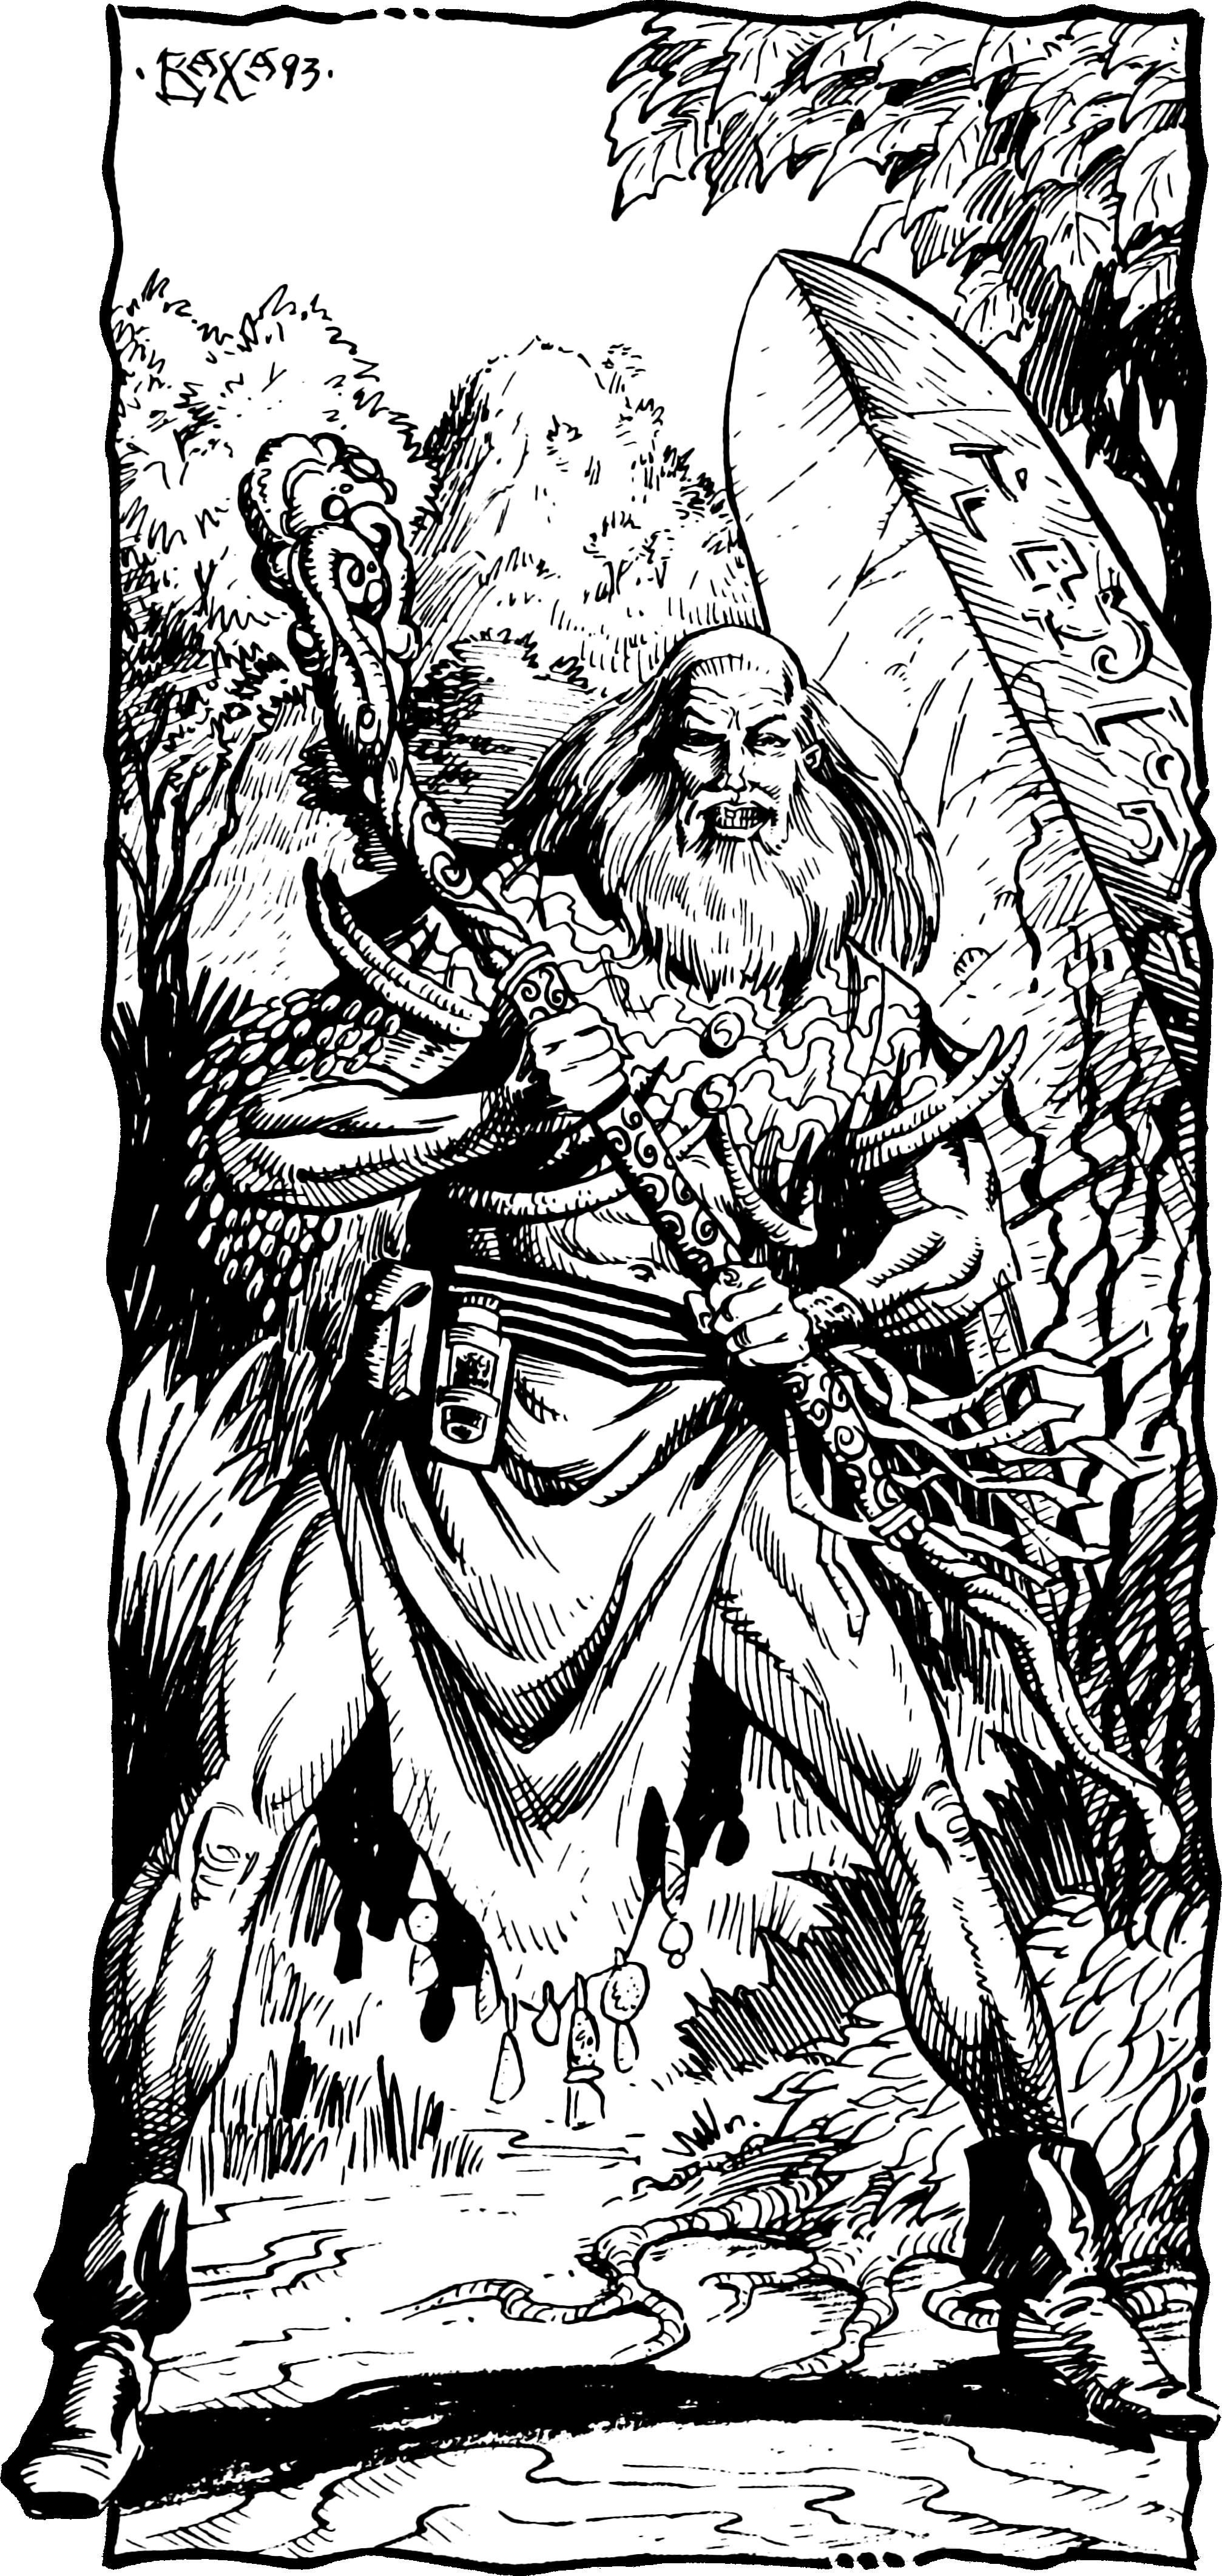
\includegraphics[width=\columnwidth]{images/druid-2.png}
\WOTC
\end{figure}

\subsubsection{Class Features}

\textbf{Weapon and Armor Proficiency:} Druids are proficient with the following weapons: alak, blowgun, club, dagger, dart, quarterstaff, scimitar, sickle, shortspear, sling, and spear. They are also proficient with all natural attacks (claw, bite, and so forth) of any form they assume with wild shape.

Druids are proficient with light and medium armor but are prohibited from wearing metal armor; thus, they may wear only padded, leather, or hide armor. (A druid may also wear wooden armor that has been altered by the ironwood spell so that it functions as though it were steel. See the ironwood spell description) Druids are proficient with shields (except tower shields) but must use only wooden ones.

A druid who wears prohibited armor or carries a prohibited shield is unable to cast druid spells or use any of her supernatural or spell-like class abilities while doing so and for 24 hours thereafter.

\textbf{Spells:} A druid casts divine spells, which are drawn from the druid spell list. Her alignment may restrict her from casting certain spells opposed to her moral or ethical beliefs; see Chaotic, Evil, Good, and Lawful Spells, below. A druid must choose and prepare her spells in advance (see below).

To prepare or cast a spell, the druid must have a Wisdom score equal to at least 10 + the spell level. The Difficulty Class for a saving throw against a druid's spell is 10 + the spell level + the druid's Wisdom modifier.

Like other spellcasters, a druid can cast only a certain number of spells of each spell level per day. Her base daily spell allotment is given on \tabref{The Druid}. In addition, she receives bonus spells per day if she has a high Wisdom score. She does not have access to any domain spells or granted powers, as a cleric does.

A druid prepares and casts spells the way a cleric does, though she cannot lose a prepared spell to cast a cure spell in its place (but see Spontaneous Casting, below). A druid may prepare and cast any spell on the druid spell list, provided that she can cast spells of  that level, but she must choose which spells to prepare during her daily meditation.

\textbf{Spontaneous Casting:} A druid can channel stored spell energy into summoning spells that she hasn't prepared ahead of time. She can ``lose'' a prepared spell in order to cast any summon nature's ally spell of the same level or lower.

\textbf{Chaotic, Evil, Good, and Lawful Spells:} A druid can't cast spells of an alignment opposed to her own. Spells associated with particular alignments are indicated by the chaos, evil, good, and law descriptors in their spell descriptions.

\textbf{Bonus Languages:} A druid's bonus language options include Sylvan, the language of woodland creatures. This choice is in addition to the bonus languages available to the character because of her race.

A druid also knows Druidic, a secret language known only to druids, which she learns upon becoming a 1st-level druid. Druidic is a free language for a druid; that is, she knows it in addition to her regular allotment of languages and it doesn't take up a language slot. Druids are forbidden to teach this language to nondruids. Druidic has its own alphabet.

% \textbf{Animal Companion (Ex):} A druid may begin play with an animal companion selected from the following list: lesser boneclaw, carru, dire rat, eagle, erdlu, jankx, jhakar, kes'trekel, kivit, owl, snake (Small or Medium viper). If the DM's campaign takes place wholly or partly in a silt environment, the DM may add silt spawn to the druid's list of options. This animal is a loyal companion that accompanies the druid on her adventures as appropriate for its kind. 

% A 1st-level druid's companion is completely typical for its kind except as noted below. As a druid advances in level, the animal's power increases as shown on the table. If a druid releases her companion from service, she may gain a new one by performing a ceremony requiring 24 uninterrupted hours of prayer. This ceremony can also replace an animal companion that has perished.

% A druid of 4th level or higher may select from alternative lists of animals. Should she select an animal companion from one of these alternative lists, the creature gains abilities as if the character's druid level were lower than it actually is. Subtract the value indicated in the appropriate list header from the character's druid level and compare the result with the druid level entry on the table to determine the animal companion's powers. (If this adjustment would reduce the druid's effective level to 0 or lower, she can't have that animal as a companion.)

\textbf{Nature Sense (Ex):} A druid gains a +2 bonus on \skill{Knowledge} (nature) and \skill{Survival} checks.

\textbf{Wild Empathy (Ex):} A druid can improve the attitude of an animal. This ability functions just like a \skill{Diplomacy} check made to improve the attitude of a person. The druid rolls 1d20 and adds her druid level and her Charisma modifier to determine the wild empathy check result. The typical domestic animal has a starting attitude of indifferent, while wild animals are usually unfriendly.

To use wild empathy, the druid and the animal must be able to study each other, which means that they must be within 9 meters of one another under normal conditions. Generally, influencing an animal in this way takes 1 minute but, as with influencing people, it might take more or less time.

A druid can also use this ability to influence a magical beast with an Intelligence score of 1 or 2, but she takes a $-4$ penalty on the check.

\textbf{Woodland Stride (Ex):} Starting at 2nd level, a druid may move through any sort of undergrowth (such as natural thorns, briars, overgrown areas, and similar terrain) at her normal speed and without taking damage or suffering any other impairment. However, thorns, briars, and overgrown areas that have been magically manipulated to impede motion still affect her.

\textbf{Trackless Step (Ex):} Starting at 3rd level, a druid leaves no trail in natural surroundings and cannot be tracked. She may choose to leave a trail if so desired.

\textbf{Nature's Speech (Su):} Starting at 4th level, a druid become able to speak with animals everywhere, as if under the effects of the \spell{speak with animals} spell.

\textbf{Wild Shape (Su):} At 5th level, a druid gains the ability to turn herself into any Small or Medium animal and back again once per day. Her options for new forms include all creatures with the animal type. This ability functions like the alternate form special ability, except as noted here. The effect lasts for 1 hour per druid level, or until she changes back. Changing form (to animal or back) is a standard action and doesn't provoke an attack of opportunity. Each time you use wild shape, you regain lost hit points as if you had rested for a night.

Any gear worn or carried by the druid melds into the new form and becomes nonfunctional. When the druid reverts to her true form, any objects previously melded into the new form reappear in the same location on her body that they previously occupied and are once again functional. Any new items worn in the assumed form fall off and land at the druid's feet.

The form chosen must be that of an animal the druid is familiar with.

A druid loses her ability to speak while in animal form because she is limited to the sounds that a normal, untrained animal can make, but she can communicate normally with other animals of the same general grouping as her new form. (The normal sound a wild parrot makes is a squawk, so changing to this form does not permit speech.)

A druid can use this ability more times per day at 6th and every three levels thereafter (9th, 12th, 15th, and 18th level). In addition, she gains the ability to take the shape of a Large animal at 9th level, a Tiny animal at 13th level, and a Huge animal at 17th level. The new form's Hit Dice can't exceed the character's druid level.

At 12th level, a druid becomes able to use wild shape to change into a plant creature with the same size restrictions as for animal forms. (A druid can't use this ability to take the form of a plant that isn't a creature.)

At 18th level, a druid becomes able to use wild shape to change into a vermin with the same size restriction as for animal forms. This transformation uses two wild shape daily uses. In addition to the normal effects of wild shape, the druid gains all the vermin's special qualities. (A druid maintains her Intelligence score and does not gain the vermin traits.)

% At 18th level, a druid becomes able to use wild shape to change into an elemental (air, earth, fire, or water) with the same size restriction as for animal forms. This transformation uses two wild shape daily uses. In addition to the normal effects of wild shape, the druid gains all the elemental's extraordinary, supernatural, and spell-like abilities. She also gains the elemental's feats for as long as she maintains the wild shape, but she retains her own creature type.

% At 18th level, a druid becomes able to assume elemental form twice per day, and at 20th level she can do so three times per day. At 20th level, a druid may use this wild shape ability to change into a Huge elemental.

\textbf{Venom Immunity (Ex):} At 8th level, a druid gains immunity to all poisons.

\textbf{A Thousand Faces (Su):} At 14th level, a druid gains the ability to change her appearance at will, as if using the \spell{disguise self} spell, but only while in her normal form. This affects the druid's body but not her possessions. It is not an illusory effect, but a minor physical alteration of the druid's appearance, within the limits described for the spell.

\textbf{Timeless Body (Ex):} After attaining 16th level, a druid no longer takes ability score penalties for aging and cannot be magically aged. Any penalties she may have already incurred, however, remain in place. Bonuses still accrue, and the druid still dies of old age when her time is up.

\subsubsection{Ex-Druids}
A druid who ceases to revere nature, changes to a prohibited alignment, or teaches the Druidic language to a nondruid loses all spells and druid abilities (not including weapon, armor, and shield proficiencies). She cannot thereafter gain levels as a druid until she atones (see the \spell{atonement} spell description).
% A druid who ceases to revere nature, changes to a prohibited alignment, or teaches the Druidic language to a nondruid loses all spells and druid abilities (including her animal companion, but not including weapon, armor, and shield proficiencies). She cannot thereafter gain levels as a druid until she atones (see the \spell{atonement} spell description).

% \subsubsection{The Druid's Animal Companion}
% A druid's animal companion is different from a normal animal of its kind in many ways. A druid's animal companion is superior to a normal animal of its kind and has special powers, as described below.

% \begin{figure}[b!]
% \centering
% 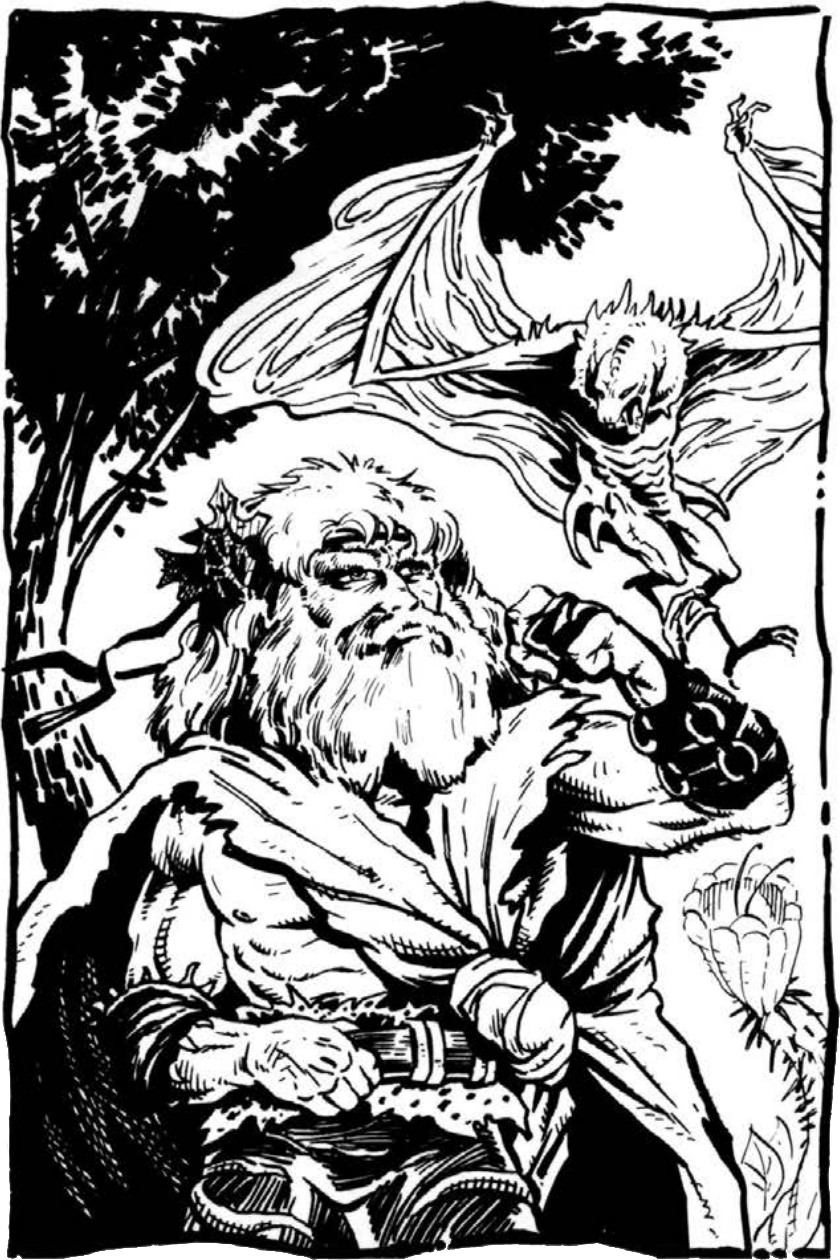
\includegraphics[width=\columnwidth]{images/druid-1.png}
% \WOTC
% \end{figure}

% \Table{}{l Z{.5cm} Z{.8cm} Z{.8cm} Z{.7cm} X}{\tableheader Class Level & \tableheader Bonus HD & \tableheader Natural Armor Adj. &\tableheader  Str/Dex Adj. &\tableheader  Bonus Tricks &\tableheader  Special\\
% 1st--2nd &&&& 1 & Link, share spells\\
% 3rd--5th & +2 & +2 & +1 & 2 & Evasion\\
% 6th--8th & +4 & +4 & +2 & 3 & Devotion\\
% 9th--11th & +6 & +6 & +3 & 4 & Multiattack\\
% 12th--14th & +8 & +8 & +4 & 5 &\\
% 15th--17th & +10 & +10 & +5 & 6 & Improved evasion\\
% 18th--20th & +12 & +12 & +6 & 7 &}

% \textbf{Animal Companion Basics:} Use the base statistics for a creature of the companion's kind, but make the following changes.

% \textbf{Class Level:} The character's druid level. The druid's class levels stack with levels of any other classes that are entitled to an animal companion for the purpose of determining the companion's abilities and the alternative lists available to the character.

% \textbf{Bonus HD:} Extra eight-sided (d8) Hit Dice, each of which gains a Constitution modifier, as normal. Remember that extra Hit Dice improve the animal companion's base attack and base save bonuses. An animal companion's base attack bonus is the same as that of a druid of a level equal to the animal's HD. An animal companion has good Fortitude and Reflex saves (treat it as a character whose level equals the animal's HD). An animal companion gains additional skill points and feats for bonus HD as normal for advancing a monster's Hit Dice.

% \textbf{Natural Armor Adj.:} The number noted here is an improvement to the animal companion's existing natural armor bonus.

% \textbf{Str/Dex Adj.:} Add this value to the animal companion's Strength and Dexterity scores.

% \textbf{Bonus Tricks:} The value given in this column is the total number of ``bonus'' tricks that the animal knows in addition to any that the druid might choose to teach it (see the \skill{Handle Animal} skill). These bonus tricks don't require any training time or \skill{Handle Animal} checks, and they don't count against the normal limit of tricks known by the animal. The druid selects these bonus tricks, and once selected, they can't be changed.

% \textbf{Link (Ex):} A druid can handle her animal companion as a free action, or push it as a move action, even if she doesn't have any ranks in the \skill{Handle Animal} skill. The druid gains a +4 circumstance bonus on all wild empathy checks and \skill{Handle Animal} checks made regarding an animal companion.

% \textbf{Share Spells (Ex):} At the druid's option, she may have any spell (but not any spell-like ability) she casts upon herself also affect her animal companion. The animal companion must be within 1.5 meter of her at the time of casting to receive the benefit. If the spell or effect has a duration other than instantaneous, it stops affecting the animal companion if the companion moves farther than 1.5 meter away and will not affect the animal again, even if it returns to the druid before the duration expires.

% Additionally, the druid may cast a spell with a target of ``You'' on her animal companion (as a touch range spell) instead of on herself. A druid and her animal companion can share spells even if the spells normally do not affect creatures of the companion's type (animal).

% \textbf{Evasion (Ex):} If an animal companion is subjected to an attack that normally allows a Reflex saving throw for half damage, it takes no damage if it makes a successful saving throw.

% \textbf{Devotion (Ex):} An animal companion gains a +4 morale bonus on Will saves against enchantment spells and effects.

% \textbf{Multiattack:} An animal companion gains \feat{Multiattack} as a bonus feat if it has three or more natural attacks and does not already have that feat. If it does not have the requisite three or more natural attacks, the animal companion instead gains a second attack with its primary natural weapon, albeit at a $-5$ penalty.

% \textbf{Improved Evasion (Ex):} When subjected to an attack that normally allows a Reflex saving throw for half damage, an animal companion takes no damage if it makes a successful saving throw and only half damage if the saving throw fails.

% \subsubsection{Alternative Animal Companions}
% A druid of sufficiently high level can select her animal companion from one of the following lists, applying the indicated adjustment to the druid's level (in parentheses) for purposes of determining the companion's characteristics and special abilities.

% Some animals are only available in certain environments. The animals available only in an aquatic environment, such as the Last Sea, are marked with $\dagger$. The animals available only in a silt environment, such as the Sea of Silt, are marked with $\diamond$.

% \Table{}{X X}{
% \multicolumn{2}{c}{\tableheader\footnotesize 4th Level or Higher (Level $-3$)}\\
% Carru, bull (6HD) & Leopard \\
% Cheetah & Lizard, giant \\
% Crodlu & Lizard, monitor\\
% Crodlu, heavy & Rasclinn\\
% Dire bat & Athasian shark$^\dagger$\\
% Erdland & Snake, constrictor\\
% Jhakar, Medium (6HD) & Snake, viper (Large)\\
% Kluzd & }

% \Table{}{X X}{
% \multicolumn{2}{c}{\tableheader\footnotesize 7th Level or Higher (Level $-6$)}\\
% Crodlu, heavy warmount & Puddingfish$^\dagger$ \\
% Inix & Lion\\
% Kalin & Lizard, subterranean\\
% Kluzd (7HD) & Snake, viper (Huge)\\
% Lirr & Takis\\
% Pterrax & Tiger}

% \Table{}{X X}{
% \multicolumn{2}{c}{\tableheader\footnotesize 10th Level or Higher (Level $-9$)}\\
% Cha'thrang & Lizard, minotaur\\
% Dire lion & Athasian shark (Huge)$^\dagger$ \\
% Hatori & Snake, giant constrictor}

% \Table{}{X X}{
% \multicolumn{2}{c}{\tableheader\footnotesize 13th Level or Higher (Level $-12$)}\\
% Lirr, large (11HD) & Athasian sloth\\
% Ruktoi$^\diamond$ & }

% \Table{}{X X}{
% \multicolumn{2}{c}{\tableheader\footnotesize 16th Level or Higher (Level $-15$)}\\
% Dire Athasian shark$^\dagger$ & Silt Horror, white$^\diamond$\\
% Dire tiger&Slimahacc\\
% Hatori, gargantuan (17HD) &}

\subsection{Playing a Druid}
You are a humanoid servant devoted to Athas and all of its elements equally. As a guardian, tender, warrior, and sometimes assassin, you further the cause of nature and help to make Athas verdant again.

You, like nature itself is neutral. You see the balance of all things. You know that every living creature is part of the food chain, and birth and death are the natural order of life. This is one of the reasons druids harbor such intense hatred for the defilers. Their magic of decay lies outside the normal cycle of life. Matter should not be destroyed, but converted to a form that will eventually return to the earth. Defiling magic destroys that which should never be destroyed, and its practice is an abomination to druids.

\subsubsection{Religion}
A druid is an individual who has devoted themselves to the balance of nature on Athas, and in particular someone who has sought out or been chosen by one of the few living spirits left in the barren land, protecting and nurturing them and the natural balance they represent.

Individual druids do not necessarily recognize one another as kin or as brothers in a religion; each conducts their affairs as they see fit in their quest to restore the balance of nature and protect their spirit's lands. Most druids recognize the various spirits as a manifestation of Athas itself, though some few more primitive or uncultured individuals or groups may believe the spirit to be a god and treat it as such.

\subsubsection{Other Classes}
Druids get along with most classes, though they despise wizards. Magic is the cause of Athas' current state, so say the druids, and while they may tolerate preservers for a short while, defilers are slain on sight. Templars are usually not welcomed by druids, as the templar is responsible for a city that encroaches on nature, and templars serve the sorcerer-kings, Athas' most powerful magic users. Elemental clerics are well received by druids, as they often share the same goals. Druids are usually at odds with paraelemental clerics, though. The paraelement proliferation on Athas is usually at the land's expense, destroying what the druid tries to accomplish.

Rangers are probably the druid's best allies. They often share the same goals, and the druid may even call upon the ranger for help in controlling a species that has become problematic or detrimental to an area. However, the ranger and the druid may sometimes be at odds, if the ranger is determined to eradicate his favored enemy while the druid seeks to protect that particular species.

\subsubsection{Combat}
Your ability to summon creatures and to turn into them is your primary weapons. Consider using them to aid your companions in flanking maneuvers, or better yet to harass enemy spellcasters (many of whom are easy to hit), especially if they are defilers. Few foes are prepared for an opponent who can call such potent beings to service, so you've also got the advantage of surprise.

Though somewhat skilled at both combat and spellcasting, you are more suited to guerrilla warfare---tracking enemies to their lair ambushing them while they sleep, or engaging in other sue surreptitious tactics. With woodland stride and trackless step, you can usually escape through the wilderness before your enemies know what hit them.

\subsubsection{Advancement}

You profit most from remaining a druid thought your advancement, so that %your animal companion and 
wild shape continue to improve as you gain levels. If you do multiclass, a level of barbarian is an excellent choice; the benefits it grants to combat and movement regardless of when you take that 1st level.

During their time of wandering, a young druid learns about the world, its ecology, the balance of nature and the ways of its creatures. After a few years of peregrination, most druids decide to settle in order to watch over a specific patch of land lands, watching over them and protecting them, and straighten their bond with a Spirit of the Land. Such druids become \class{Grove Masters}.

\subsection{Starting Packages}
\subsubsection{The Beastmaster}

Half-Elf Druid

\textbf{Ability Scores:} Str 10, Dex 15, Con 12, Int 8, Wis 15, Cha 12.

\textbf{Skills:} \skill{Handle Animal}, \skill{Hide}, \skill{Survival}.

\textbf{Languages:} Common, Elven.

\textbf{Feat:} \feat{Animal Affinity}.

\textbf{Weapons:} Longspear (1d8/$\times$3)

Sling with 20 bullets (1d4, 15 m).

\textbf{Armor:} Hide (+3 AC).

\textbf{Gear:} Spell component pouch, standard adventurer's kit, 20 cp.

\textbf{Class Features:} Jankx animal companion.

\textbf{Spells Prepared:} 1st---\spell{cure light wounds}, \spell{speak with animals}; 0---\spell{cure minor wounds} (2), \spell{defiler scent}.

\subsubsection{The Defiler Hunter}

Human Druid

\textbf{Ability Scores:} Str 13, Dex 14, Con 12, Int 10, Wis 15, Cha 8.

\textbf{Skills:} \skill{Concentration}, \skill{Hide}, \skill{Listen}, \skill{Move Silently}, \skill{Spot}, \skill{Survival}.

\textbf{Languages:} Common

\textbf{Feat:} \feat{Defender of the Land}, \feat{Track}.

\textbf{Weapons:} Spear (1d8/$\times$3, 6m)

Sling with 20 bullets (1d4, 15 m).

\textbf{Armor:} Hide (+3 AC).

\textbf{Gear:} Spell component pouch, standard adventurer's kit, 20 cp.

\textbf{Class Features:} Jhakar animal companion.

\textbf{Spells Prepared:} 1st---\spell{backlash}, \spell{longstrider};\hskip10pt 0---\spell{cure minor wounds}, \spell{defiler scent} (2).

\subsubsection{The Warden}

Pterran Druid

\textbf{Ability Scores:} Str 8, Dex 11, Con 14, Int 10, Wis 17, Cha 14.

\textbf{Skills:} \skill{Hide}, \skill{Knowledge} (nature), \skill{Move Silently}, \skill{Spot}, \skill{Survival}.

\textbf{Languages:} Saurian.

\textbf{Feat:} \feat{Spell Focus} (conjuration).

\textbf{Weapons:} Alak (1d6/$\times$3)

Blowgun with 20 needles (1, 3 m).

\textbf{Armor:} Leather (+2 AC), light wooden shield (+1 AC).

\textbf{Gear:} Spell component pouch, standard adventurer's kit, 20 cp.

\textbf{Class Features:} Lesser boneclaw animal companion.

\textbf{Spells Prepared:} 1st---\spell{entangle}, \spell{plant renewal}; 0---\spell{defiler scent}, \spell{detect magic}, \spell{nurturing seeds}.

\subsection{Druids on Athas}
\Quote{The druids are no longer hunted in force by the sorcerer-kings. The kings believe there simply aren't enough left to threaten them. But the templars, and even some elves I know, have been well rewarded for delivering the heads of wasteland druids.}{Jurgan, Urikite earth cleric}

Perhaps the only thing rarer to see in Athas than a wizard is a druid. After centuries of persecution, they were forced to either die in the hands of the agents of the sorcerer-monarchs, or to watch their beloved land wither and die before their eyes.

Because of that, druids are usually loners and avert to social interaction. They live off the land, within the land, and they have sacrificed their entire lives for the land, very little besides it occupies the mind of a druid.

\subsubsection{Daily Life}

A druid adventures to learn about Athas, to protect nature, and to further his own aims. Druids usually spend their days in contemplation of nature, and tending their lands; one may watch over a particular stretch of open desert, another may protect a belt of scrub grass within it, while still another might watch over a small oasis that borders on both, always hidden and always watching.

The Athasian druid is a wanderer who hunts down a powerful defiler that has despoiled the wastes, or a visionary who tends the land and teaches the local population how to live in harmony with their surroundings. The Athasian druid fights for an almost lost cause, and it matters not if that cause is revenge himself against those who destroyed his land and friends or a ceaseless desire to bring green and hope to Athas.

\subsubsection{Notables}

Druids very rarely become famous, since they usually avoid social interaction combined the fact that it might put their lives at risk since usually sorcerer-kings and defiler usually put a reward for the head of a notorious or troublesome druid. A legend claim that Mearedes the druidess came to the island of Shault when its forest was all but dead and she managed to nurture it back to its vibrant health.

\subsubsection{Organizations}

Ever since the Eradication, an anti-druidic jihad led by sorcerer-kings more than 1,500 years ago, no specific druidic organization exists, although some form temporary alliances with Veiled Alliance members from time to time. Legends say that the druids who remained after the Eradication gathered on a high mesa somewhere in the northern Tablelands. It was there they decided that they should scatter to the most remote reaches and farthest regions of Athas, there to bide their time, waiting for the day when they were powerful enough to challenge the sorcerer-kings again. This was a long time ago, and the druids have yet to return to the cities of the defilers. Some say that they will never return and that their seclusion and isolation have destroyed whatever power they once wielded as a circle. Others say that the druid's long wait is indicative of their cunning, and that their plan is to insure that the next confrontation with the kings won't end in defeat.

\subsubsection{NPC Reactions}

Druids are natural loners, and usually avoid social interactions unless they have to. In such cases, those who are directly benefited from the druid's work of tending the land begin two steps nearer helpful, while defilers and evil paraelemental clerics begin two steps nearer hostile.

\subsubsection{Druid Lore}

Characters with ranks in \skill{Knowledge} (nature) can research druids to learn more about them. When a character makes a skill check, read or paraphrase the following, including the information from lower DCs.

\textbf{DC 10:} Druids devote themselves to the land, drawing off their power straight from Athas itself.

\textbf{DC 15:} Druids from a mystical connection to mysterious beings known as Spirits of the Land. They hate all defilers and those who abuse the land.

\textbf{DC 20:} Druids are masters of the forces of nature, being able to transform into the creatures that dwell in their lands, and some even learn to counter the destruction of defilement.

\Class{Fighter}
{Any wastelander can pick up a bone and call it a club, but try pitting fifty of those against one dozen trained soldiers, and maybe you'll have an even match.}{Nikolos, human fighter}

From the small forts in sandy wastes of Athas to the guards of the merchant houses in the city-states, fighters are Athas' most common sight. Whether it is as mercenaries for the sorcerer-kings or as hired guards protecting the wealth of the nobility, fighters can be found everywhere in the Tablelands. Athas' fighters are trained to fight in small groups or huge units. Those that have proven themselves become the commanders in the city-states' armies, commanding hundreds or even thousands of men into war.

\subsection{Making a Fighter}
Fighters receive the best allotment of fighting skills and abilities. They learn the use of most weapons, the best armors and shields, as well as gaining special abilities to use with these weapons and armor.

Some fighters specialize in using a single weapon, and become masters at its use and deadliness. Other fighters will prefer more rounded skills, learning to shoot from far with bows and arrows, or nets or spears. Regardless, the fighter is to be feared.

\textbf{Races:} All of Athas' races can become fighters. Humans are usually the most numerous, though, since they are the most numerous of the races of the Tablelands. Dwarves make good fighters, even though they are smaller than most races; their inborn toughness and great strength more than makes up for their smaller stature. The half-giants are also seen very often as fighters, since their great strength and size are perfect for the job. Muls, with the inherited traits of both humans and dwarves, are also great fighters. Elves, with their long legs and frail constitution, are not often seen as fighters. Athas' intelligent insects, the Thri-kreen, make excellent warriors, with their four arms and the fact they do not need to sleep. Many of the savage races of the Tablelands are fighters, although most become rangers in order to survive.

\textbf{Alignment:} Fighters come from all walks of life, and can be of any alignment. Good fighters are usually seen as the protectors of small villagers or are part of renegade slave tribes, helping their tribe to survive in the harsh desert. Or they can be found as a dwarf perhaps, whose focus it is to guard his fellows. Evil fighters are often part of mercenary bands or under the control of a sorcerer-king; these beings often fight for power and money. Evil fighters can also be found as the rulers of small forts, guarding their oasis and exacting a hefty toll for its use.

\Figure{t}{images/fighter-3.png}

\MiniWarriorTable{The Fighter}{
1st  & +1             & +2  & +0 & +0 & Bonus feat \\
2nd  & +2             & +3  & +0 & +0 & Bonus feat \\
3rd  & +3             & +3  & +1 & +1 &  \\
4th  & +4             & +4  & +1 & +1 & Bonus feat \\
5th  & +5             & +4  & +1 & +1 & Martial prowess \\
6th  & +6/+1          & +5  & +2 & +2 & Bonus feat \\
7th  & +7/+2          & +5  & +2 & +2 & Martial prowess \\
8th  & +8/+3          & +6  & +2 & +2 & Bonus feat \\
9th  & +9/+4          & +6  & +3 & +3 & Martial prowess \\
10th & +10/+5         & +7  & +3 & +3 & Bonus feat \\
11th & +11/+6/+1      & +7  & +3 & +3 & Martial prowess \\
12th & +12/+7/+2      & +8  & +4 & +4 & Bonus feat \\
13th & +13/+8/+3      & +8  & +4 & +4 & Martial prowess \\
14th & +14/+9/+4      & +9  & +4 & +4 & Bonus feat \\
15th & +15/+10/+5     & +9  & +5 & +5 & Martial prowess \\
16th & +16/+11/+6/+1  & +10 & +5 & +5 & Bonus feat \\
17th & +17/+12/+7/+2  & +10 & +5 & +5 & Martial prowess \\
18th & +18/+13/+8/+3  & +11 & +6 & +6 & Bonus feat \\
19th & +19/+14/+9/+4  & +11 & +6 & +6 & Martial prowess \\
20th & +20/+15/+10/+5 & +12 & +6 & +6 & Bonus feat \\
}

\subsection{Game Rule Information}
\textbf{Hit Die:} d10.

\subsubsection{Class Skills}
\skill{Autohypnosis} (Wis), \skill{Climb} (Str), \skill{Craft} (Int), \skill{Handle Animal} (Cha), \skill{Intimidate} (Cha), \skill{Jump} (Str), \skill{Knowledge} (warcraft) (Int), \skill{Ride} (Dex), and \skill{Spot} (Wis).

\textbf{Skill Points per Level:} 4 + Int modifier ($\times4$ at 1st level).

\subsubsection{Class Features}
\textbf{Weapon and Armor Proficiency:} A fighter is proficient with all simple and martial weapons and with all armor (heavy, medium, and light) and shields (including tower shields).

\textbf{Bonus Feats:} At 1st level, a fighter gets a bonus combat-oriented feat in addition to the feat that any 1st-level character gets and the bonus feat granted to a human character. The fighter gains an additional bonus feat at 2nd level and every two fighter levels thereafter (4th, 6th, 8th, 10th, 12th, 14th, 16th, 18th, and 20th). These bonus feats must be drawn from the feats noted as fighter bonus feats. A fighter must still meet all prerequisites for a bonus feat, including ability score and base attack bonus minimums.

These bonus feats are in addition to the feat that a character of any class gets from advancing levels. A fighter is not limited to the list of fighter bonus feats when choosing these feats.

\textbf{Martial Prowess:} At 5th level and every two levels thereafter, a fighter improves his repertoire with new techniques. He may choose one of the following options.

\textit{Active Defense (Ex):} A fighter gains a dodge bonus to AC equal to \onequarter his fighter levels when wielding a shield and fighting defensively or using the \feat{Combat Expertise} feat. When using total defense, this bonus increases to \onehalf his fighter levels.

\textit{Aim (Ex):} A fighter can take full-round action to make a \skill{Spot} check to improve his next attack against a specific foe. DC is equal to his target's AC. His next attack against the target ignore armor bonus and natural armor bonus. This attack must be made within a number of rounds equal to \onequarter his fighter levels.

\Figure*{t}{images/battle-1.png}

\textit{Ambidextrous (Ex):} A fighter may add his full Strength modifier to his off-hand weapon damage, instead of \onehalf his Strength bonus.

\textit{Bravery (Ex):} A fighter with this ability gains a bonus equal to \onehalf his fighter levels on Will saves against mind-affecting abilities.

\textit{Close Combat Shot (Ex):} A fighter can attack with a ranged weapon while in a threatened square and not provoke an attack of opportunity.

\textit{Commanding Strike (Ex):} A fighter may forgo his attack with the lowest base attack bonus in a total attack to create an opening for an ally. The designated ally may use one of his attacks of opportunity to strike a foe. The ally may use ranged attacks---this is an exception for the rules for attacks of opportunity.

\textit{Coordinate Allies (Ex):} A fighter can use a full-round action to identify and apply an effective tactic for his allies. Each creature to be affected must be able to see and hear him, and able to pay attention to him. To coordinate, the fighter must make a \skill{Knowledge} (warcraft) check with a DC equal to 15 + the number of allies affected. If the check succeeds, all affected allies gain a competence bonus on attack rolls or a dodge bonus to AC equal to \onequarter his fighter levels. He chooses which of the two benefits to impart and must impart the same benefit to all affected allies. The benefits last for 1 round. The fighter cannot use this ability on himself.

\textit{Crossbowman (Ex):} Whenever a fighter attacks with a crossbow as a readied action, his target is denied its Dexterity bonus to its AC.

\textit{Defensive Tactics (Ex):} A fighter may use a move action to coordinate his allies to a defensive maneuver. Each creature to be affected must be able to see and hear him, and able to pay attention to him. To coordinate, the fighter must make a \skill{Knowledge} (warcraft) check with a DC equal to 10 + the number of allies affected. If the check succeeds, all affected allies gain a moral bonus to AC against attacks of opportunity equal to \onequarter his fighter levels. The benefits last for 1 round.

\textit{Double Opportunity (Ex):} When a fighter makes an attack of opportunity, he may attack once with both his primary and secondary weapons. The penalties for attacking with two weapons apply normally. The fighter must be at least 11th level to select this technique.

\textit{Flanking Tactics (Ex):} A fighter may use a move action to coordinate his allies to a flanking maneuver against a target. Each creature to be affected must be able to see and hear him, and able to pay attention to him. To coordinate, the fighter must make a \skill{Knowledge} (warcraft) check with a DC equal to the target's Base Attack Bonus. If the check succeeds, all affected allies gain a competence bonus on damage rolls equal to \onequarter his fighter levels when they flank the target. The benefits last for 1 round. The fighter cannot use this ability on himself.

\textit{Harden Resolve (Ex):} A fighter may use a standard action to improve his allies' morale. Each creature to be affected must be able to see and hear him, and able to pay attention to him. To coordinate, the fighter must make a \skill{Knowledge} (warcraft) check with a DC equal to 25 + 2 for each ally affected. If the check succeeds, all affected allies gain damage reduction equal to \onequarter his fighter levels. If an ally already has damage reduction, it improves by the same amount. The benefits last for 1 round. A fighter must be at least 11th level to select this technique.

\textit{Hawkeye (Ex):} Whenever a fighter isn't flat-footed, he has advantage on \skill{Spot} checks.

\textit{Lead the Charge (Ex):} A fighter may make a \skill{Knowledge} (warcraft) check during a charge against one specific foe. The check DC is equal to 20 + the number of allies affected. If the check succeeds, all affected allies that charge the same foe gain a competence bonus on attack and damage rolls equal to \onequarter his fighter levels. The benefits last for 1 round.

\textit{Leadership:} A fighter may gain the \feat{Leadership} feat as a bonus feat.

\textit{Maneuvering Attack (Ex):} A fighter may forgo his attack with the lowest base attack bonus in a total attack to maneuver one of his comrades into a more advantageous position. The fighter chooses a friendly creature that can see and hear him. That creature can use an immediate action to move up to half its speed.

\textit{Martial Versatility (Ex):} A fighter can apply any feat he has that affects only one weapon type (such as, \feat{Weapon Focus} or \feat{Rapid Reload}) to any simple weapon. A fighter must be at least 11th level to select this technique.

\textit{Mirror Move (Ex):} A fighter gains \onequarter his fighter levels as an insight bonus to AC when attacked by any weapon with which he has the \feat{Weapon Specialization} feat.

\textit{Overhand Chop (Ex):} When a fighter makes a single attack (with the attack action or a charge) with a two-handed weapon, he adds triple his Strength bonus on damage rolls, instead of 1\onehalf his Strength bonus.

\textit{Phalanx (Ex):} As long as a fighter is wielding a shield, he may use any two-handed polearm or spear as if it was an one-handed weapon. A fighter cannot use this ability with a buckler.

\textit{Pressing Shield (Ex):} A fighter may use his shield to help with his bull rush and overrun attempts. He adds his shield bonus on Strength checks made to push back the defender, and on Strength checks to knock down his opponent. A fighter cannot use this ability with a buckler.

\textit{Quick Aid (Ex):} A fighter may use the aid another action with a full attack. He must use his attack with the highest base attack bonus and roll against AC 20.

\textit{Ready Polearm (Ex):} A fighter can ready any weapon that deals increased damage against charge as an immediate action. A fighter must be at least 11th level to select this technique.

\textit{Second Wind (Ex):} A fighter with this ability can dig his resolve and endurance to find an extra burst of vitality. He can use a standard action to gain a number of temporary hit points equal to his Constitution modifier $\times$ his fighter levels. These hit points last until for the end of the encounter. He can use this ability only once per encounter.

\textit{Shield Another (Ex):} A fighter can use his shield to protect an adjacent ally. When using aid another to grant AC to an ally, he can choose a number to add as penalty to his shield bonus until his next turn. The ally target of the aid another action gains improves their shield bonus by that number. The fighter can't choose a number greater than his shield bonus or his base attack bonus. A fighter cannot use this ability with a buckler.

\textit{Shorten Haft (Ex):} A fighter may threaten adjacent squares when wielding reach weapons.

\textit{Skirmisher (Ex):} Whenever a fighter moves 3 or more meters in his turn, he gains a dodge bonus against ranged attacks equal to \onequarter his fighter.

\textit{Tortoise Style (Ex):} While wielding a shield, the fighter improves his shield bonus by \onequarter his fighter levels. A fighter cannot use this ability with a buckler.

\textit{Two-handed Style (Ex):} When the fighter rolls a 1 or 2 on a damage die for an attack made with a melee weapon wielded with two hands, he can reroll the die and must use the new roll even if the new roll is a 1 or 2. The fighter cannot use this benefit with light weapons.

\textit{Uncanny Dodge (Ex):} A fighter can react to danger before his senses would normally allow his to do so. He retains his Dexterity bonus to AC (if any) even if he is caught flat-footed or struck by an invisible attacker. However, he still loses his Dexterity bonus to AC if immobilized. If a fighter already has uncanny dodge from a different class he automatically gains improved uncanny dodge instead.

\textit{Weapon Training (Ex):} A fighter improves his aptitude in martial weapons. He gains a competence bonus on his attack rolls equal to \onequarter his fighter levels, whenever he is wielding a simple or martial weapon.


\subsection{Playing a Fighter}
Playing an Athasian fighter is not much different than playing one in other settings, the only difference is that the extreme heat makes most armor less than desirable on Athas.

As a fighter, you undertake adventures according to the dictates of your cause, your faith, or your own selfish needs. You might find yourself on the hot, sandy field of battle, charging shoulder to shoulder with peasants and soldiers, raising pitchforks and shields against the defilers of the enemy army.

\subsubsection{Religion}
There are no gods on Athas, but many fighters worship the sorcerer-king of their respective cities as gods. Some fighters pay homage to the elemental forces of the Tablelands, asking their favored element for luck before entering the battlefield.

\subsubsection{Other Classes}
Fighters get along with most other classes. The rangers of the Tablelands often receive the highest of the respect for their ability to survive the wastes. Gladiators and fighters are often at each other's throats, since both share great combat abilities but differ in their methodology; they often try to show how each is better than the other is. Elemental clerics are welcome for their healing abilities as well as the help they can provide in battle.

Fighters are uneasy around wizards; like the rest of the population they distrust magic. Templars are also distrusted, for the same reasons everyone else distrusts templars. Rogues are usually scorned by fighters; they prefer open battle to the rogue's sneaky ways.

\subsubsection{Combat}
Your specific tactics in battle depend on your role in the party and your weapon of choice. However, certain tactics are common to all fighters.

You are generally at the forefront of any battle. Fighting on the front line allows you maximize your combat feats. Furthermore, if opponents focus on you, they cannot injure your allies. As a fighter, you're at your best when you can take on the monster or opponent that deals the most damage.

\subsubsection{Advancement}
When looking at feats to select as you gain levels, you have two basic paths. You can focus on your fighting skills, or you can attempt to expand your capabilities to serve as the party's leader. The former option is best when you are the group's primary combat specialist. If the party includes another fighter or suitable melee character, you can afford to dabble in Charisma-based skills. Although Diplomacy is not a class skill for you, the Field Office feat combined with a few cross-class ranks makes you a serviceable emissary.

When it comes to combat feats, look to ones that improve your ability to deal damage. Feats such as Power Attack, Weapon Focus, and so forth are excellent options to boost your offense. Concentrated Fire, Rotate Lines, Shield Wall, and Spear Wall are excellent feats for army fighters.

Improved Initiative is a critically important feat, since it allows you to act first, move forward and defend or guide your allies. The sooner you find a place in the front line, the longer you can hold back the enemy.


\subsection{Starting Packages}
\subsubsection{The Archer}
Elf Fighter

\textbf{Ability Scores:} Str 15, Dex 16, Con 11, Int 10, Wis 12, Cha 8.

\textbf{Skills:} \skill{Jump}, \skill{Spot} (cc).

\textbf{Languages:} Common, Elven.

\textbf{Feat:} \feat{Point Blank Shot}, \feat{Precise Shot}.

\textbf{Weapons:} Macahuitl (1d8/19-20)

Dagger (1d4/19-20, 3 m)

Longbow with 40 arrows (1d8/$\times$3, 30 m).

\textbf{Armor:} Chitin armor (+4 AC).

\textbf{Gear:} Standard adventurer's kit, 11 cp.

\subsubsection{The Defender}
Dwarf Fighter

\textbf{Ability Scores:} Str 15, Dex 13, Con 16, Int 10, Wis 12, Cha 8.

\textbf{Skills:} \skill{Craft} (weaponsmithing), \skill{Knowledge} (warcraft), \skill{Intimidate}.

\textbf{Languages:} Common, Dwarven.

\textbf{Feat:} \feat{Disciplined}, \feat{Weapon Focus} (dwarven waraxe).

\textbf{Weapons:} Dwarven waraxe (1d10/$\times$3)

Shortbow with 20 arrows (1d6/$\times$3, 18 m).

\textbf{Armor:} Scale mail (+4 AC), heavy wooden shield (+2 AC).

\textbf{Gear:} Standard adventurer's kit, 42 cp.

\subsubsection{The Leader}
Human Fighter

\textbf{Ability Scores:} Str 15, Dex 8, Con 13, Int 10, Wis 12, Cha 14.

\textbf{Skills:} \skill{Diplomacy} (cc), \skill{Knowledge} (warcraft), \skill{Intimidate}.

\textbf{Languages:} Common.

\textbf{Feat:} \feat{Field Officer}, \feat{Inspiring Presence}, \feat{Weapon Focus} (great macahuitl).

\textbf{Weapons:} Great macahuitl (2d6, 19-20)

Shortbow with 20 arrows (1d6/$\times$3, 18).

\textbf{Armor:} Scale mail (+4 AC).

\textbf{Gear:} Standard adventurer's kit, 19 cp.


\subsection{Fighters on Athas}
\Quote[-.em]{Yeah, he was alright with a sword, but he would wet himself every time we walked out onto the sand of the arena. I think it was the crowd... or the goat-headed giant they paired us against. Poor little weed, he never saw that club coming.}{Grek the Grand, talking about his onetime matched pair contest with Slavek Thydor}

Fighters bring clashing weapons, stirring speeches, and mass combat to the campaign. On Athas, the fighter is a trained warrior, a soldier skilled in mass warfare. Every society on Athas maintains an army of fighters to protect itself from attack or to wage wars of plunder and annihilation against its neighbors. Fighters are both the commanders and soldiers in these armies, and at higher levels are experts in both individual and formation combat, leadership, and morale.

\subsubsection{Daily Life}
A fighter adventures to prove his superior skill at arms, to advance the cause of whatever master he might serve, and to further his own aims.

Once he has reached a respectable level of accomplishment, a fighter might take the Leadership feat and start building his own army. As word spreads, less experienced warriors who are eager to fight for the same causes seek him out as the desperate peoples of Athas constantly look for great commanders, warriors who will lead them.

\subsubsection{Notables}
Fighters can notoriety for their deeds, whether triumphs in combat, selfless acts of great honor, or great tyranny. Many an adventurer grew up on stories such as that of the Crimson Legion, and how it managed to defeat Urik's previously undefeated army.

Another legend tells of about the rise and fall of General Zanthiros, the leader of the Balican army who managed to save the city from an onslaught of beast-headed giants more than once, and after losing the elections, left the city with hundreds of soldiers loyal to him and formed a raiding tribe.

\subsubsection{Organizations}
Fighters often band together into small armies or as mercenary groups working for trade houses. These organizations typically have different credos and values, but they allow their members to focus their time on their individual quests.

\subsubsection{NPC Reactions}
Individuals react to fighters based on their previous interactions with other members of the class. A brave fighter meets cold silence and contempt around the Barrier Wastes where evil fighters oppress the populace.

Gladiators usually talk down on fighters, saying that gladiators are the true masters of combat. Fighters usually reply that gladiators are nothing without a crowd looking. Because of that, their initial reaction is one step towards unfriendly than normal.

A fighter who has lived long enough to retire from adventuring typically acquires some position of authority, with commensurate political power, whether as a caravan leader, army general, or ruler of a raiding or slave tribe.

\subsubsection{Fighter Lore}
Characters with ranks in \skill{Knowledge} (warcraft) can research fighters to learn more about them. When a character makes a skill check, read or paraphrase the following, including the information from lower DCs.

\textbf{DC 10:} Fighters may not be as flashy as gladiators in combat, but they surely are more effective in mass combat.

\textbf{DC 15:} Fighters are combat-oriented characters adept at hand-on-hand combat just as well as commanding entire armies.

\textbf{DC 20:} A fighter's mere presence in the battlefield can be enough to inspire his soldiers and weaken the resolve of his enemies.

\Class{Gladiator}
{I might be a slave, but I am famous, I dine well, and my company is that of the finest noble women. Tell me, what do you have that I do not, slave trader---except the freedom to feel miserable?}{Jarek, arena champion}

\begin{figure}[t!]
\centering
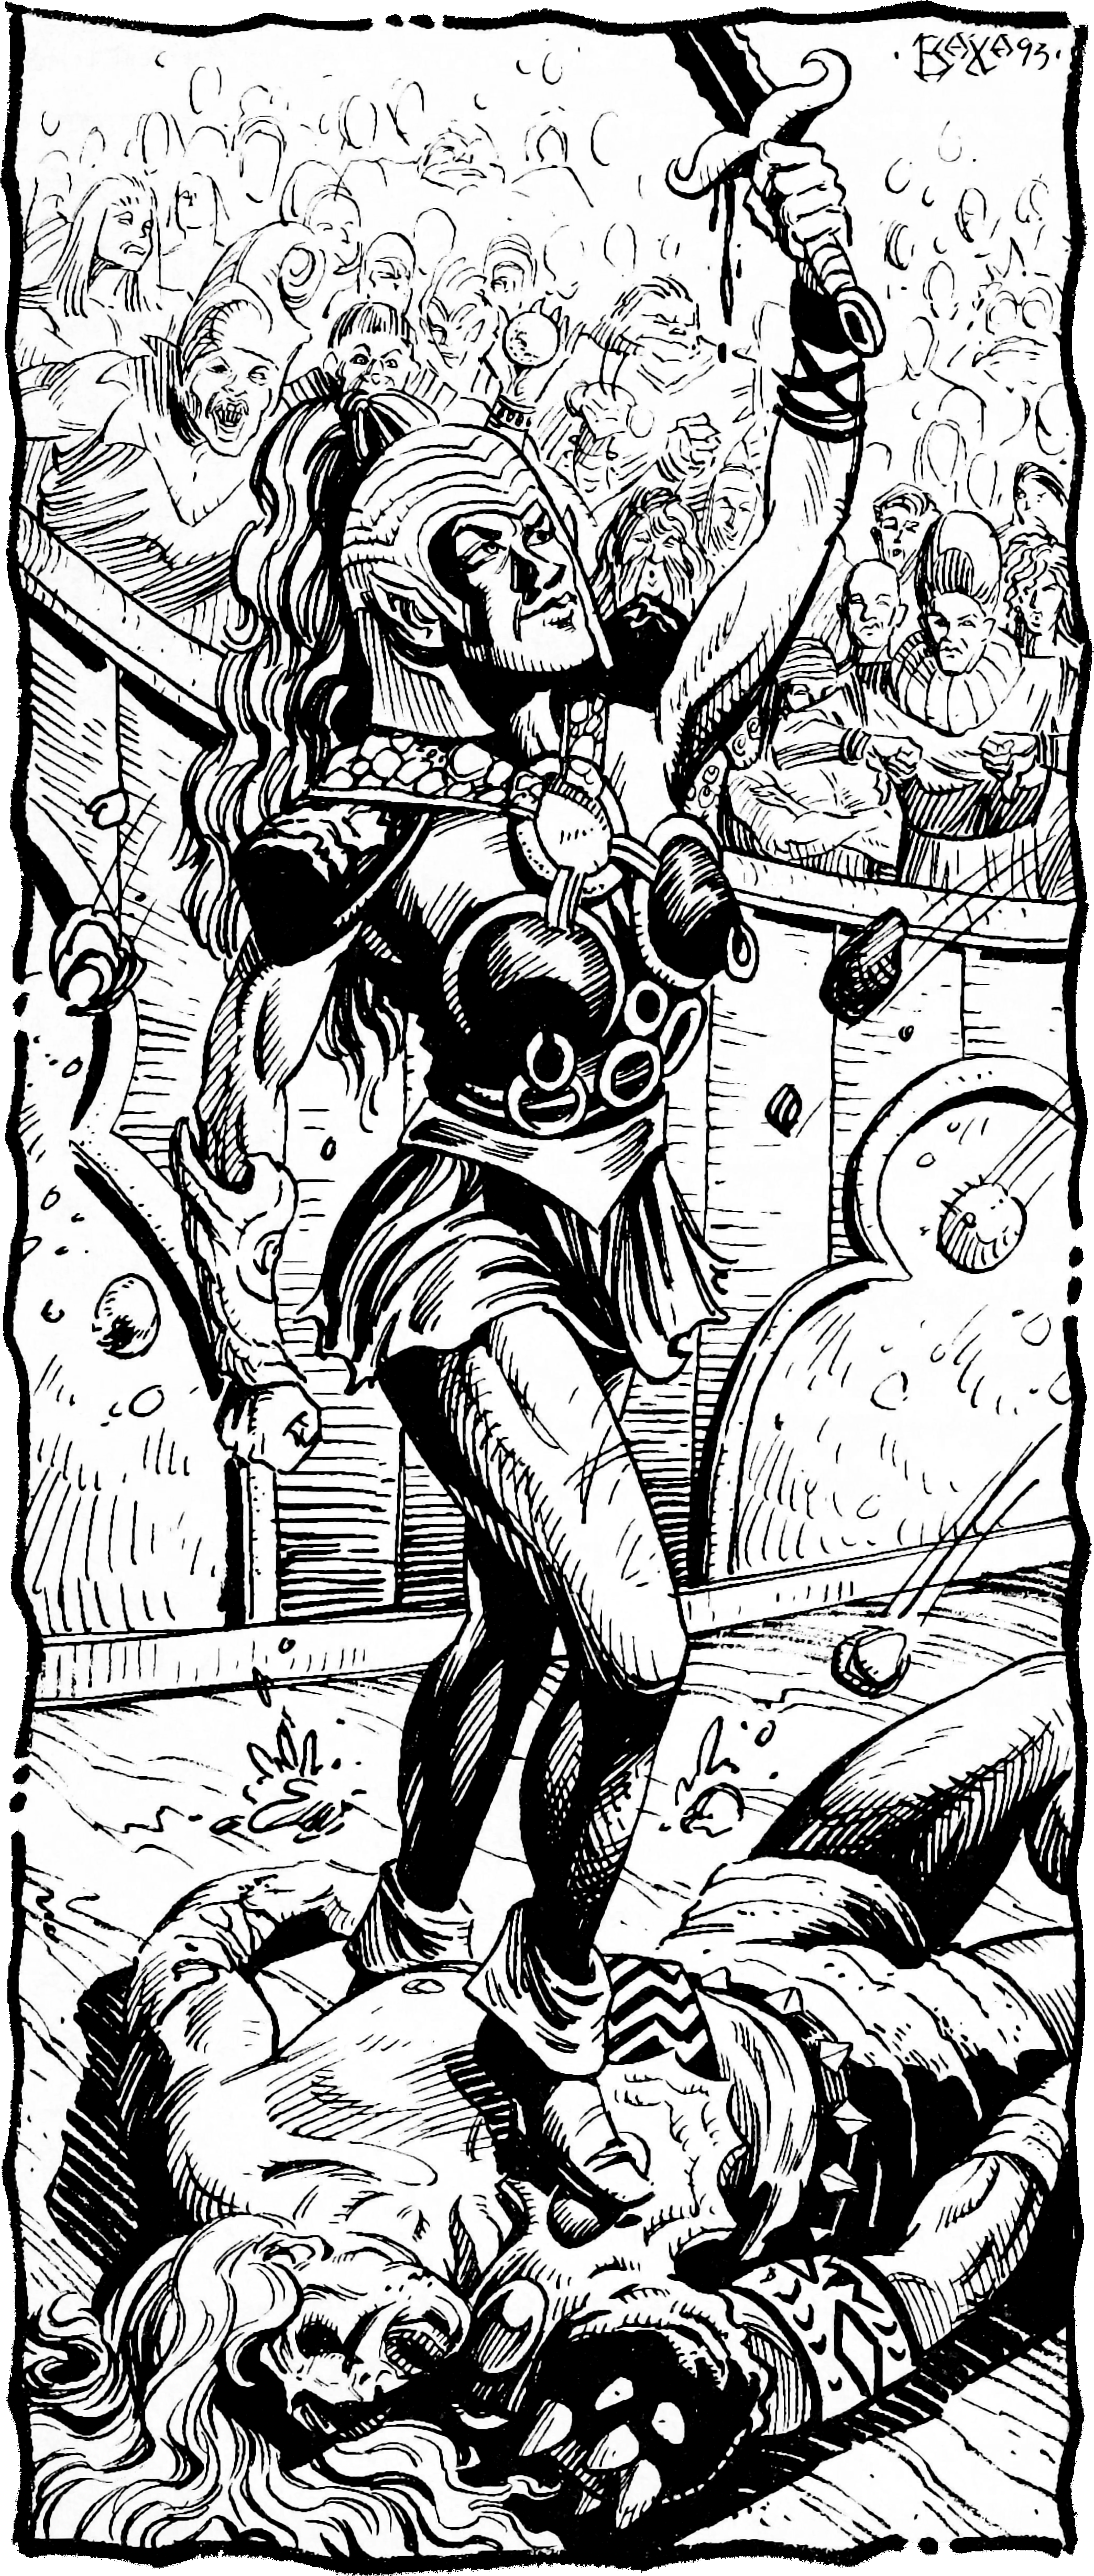
\includegraphics[width=\columnwidth]{images/gladiator-2.png}
\WOTC
\end{figure}

The arena is the battlefield of the gladiator. From hand-to-hand combat in the mud pits of small forts to the grand games of the city-states, the gladiator is a warrior who fights to the sounds of people cheering his name or cursing his presence. A master of crowd control and the art of prolonged combat, gladiators are trained to fight.

They train to best wild beasts in deadly games for the amusement of the masses. They fight for glory, wealth, prestige and power. They fight to survive. Some are merely slaves, having to fight and perhaps hoping to win a chance to obtain freedom, while some fight willingly for the thrill of combat or the promise of riches and fame.

\WarriorTable[ll *{3}{C} p{8cm}]{The Gladiator}{
1  & +1             & +2  & +0 & +0 & Unarmed strike, gladiatorial performance, dirty trick +1/$-1$                 \\
2  & +2             & +3  & +0 & +0 & Bonus feat, exotic weapon, stance (arena guile)                               \\
3  & +3             & +3  & +1 & +1 & Bonus feat, exotic aptitude, taunt                                            \\
4  & +4             & +4  & +1 & +1 & Uncanny dodge                                                                 \\
5  & +5             & +4  & +1 & +1 & Armor optimization 1, \feat{Improved Feint}                                   \\
6  & +6/+1          & +5  & +2 & +2 & Exotic weapon, parry, shake off                                               \\
7  & +7/+2          & +5  & +2 & +2 & Bonus feat, dirty trick +2/$-2$, stance (threatening glare, defensive stance) \\
8  & +8/+3          & +6  & +2 & +2 & Improved uncanny dodge, mercy                                                 \\
9  & +9/+4          & +6  & +3 & +3 & \feat{Leadership}, pounce                                                     \\
10 & +10/+5         & +7  & +3 & +3 & Armor optimization 2, exotic weapon                                           \\
11 & +11/+6/+1      & +7  & +3 & +3 & Improved parry                                                                \\
12 & +12/+7/+2      & +8  & +4 & +4 & Dragon's fury, stance (keen eye, scoundrel pose)                              \\
13 & +13/+8/+3      & +8  & +4 & +4 & Dirty trick +3/$-3$, greater feint                                            \\
14 & +14/+9/+4      & +9  & +4 & +4 & Exotic weapon                                                                 \\
15 & +15/+10/+5     & +9  & +5 & +5 & Armor optimization 3, dragon's speed                                          \\
16 & +16/+11/+6/+1  & +10 & +5 & +5 & Greater parry                                                                 \\
17 & +17/+12/+7/+2  & +10 & +5 & +5 & Stance (balancing dance, hypnotic fortitude)                                  \\
18 & +18/+13/+8/+3  & +11 & +6 & +6 & Exotic weapon, mindless focus                                                 \\
19 & +19/+14/+9/+4  & +11 & +6 & +6 & Dirty trick +4/$-4$                                                           \\
20 & +20/+15/+10/+5 & +12 & +6 & +6 & Armor optimization 4                                                          \\
}


\subsection{Making a Gladiator}
Gladiators are among the best one-on-one fighters in all the Tablelands. They are trained in hand-to-hand combat before moving on to the use of exotic weapons of the arena. They learn to improvise weapons, wielding broken bones or wooden shafts with deadly precision. They learn how to taunt and tease opponents, driving them to reckless acts and taking advantage of the situation to strike down or maim a foe.

After all, a long, drawn-out combat is more a crowd pleaser than a ten-second bout.

\textbf{Abilities:} Strength and Constitution are vital to a gladiator, since he is often in harm's way. Intelligence is useful for gaining plenty of skills points, which a gladiator needs to purchase Bluff, Intimidate, Performance, and Sense Motive, key skills for any arena performer.

\textbf{Races:} All races of Athas can be found in the arenas of the Tablelands. Muls, with their mixed dwarven and human parentage, are highly prized in the arenas. They are often bought for a high price and treated well in return for victory on the combat floor. Elves are often used for their swiftness and natural flair for taunting their opponent. Humans are the most common of gladiators, since humans are the most common race in the Tablelands. Halflings make poor gladiators, since they abhor slavery and will usually starve themselves to death rather than being used as commodities by anyone. The savage races of the wastes are often used as gladiators, usually as fodder for the most successful gladiators, though those demonstrating excellent combat prowess receive formal training.

\textbf{Alignment:} Gladiators are of all alignments. Some gladiators will obey all arena rules, being lawful individuals, though these often do not last long in the arena. Many gladiators tend toward a chaotic alignment. Evil gladiators use dirty tricks to gain an advantage over an opponent. Gladiators of all alignments can become crowd favorites, increasing their chances of winning their matches, since often times these matches are prearranged. The intrigues of the city-states can reach deep into the arena.

\subsection{Game Rule Information}

\textbf{Hit Die:} d8.

\subsubsection{Class Skills}
\skill{Autohypnosis} (Wis), \skill{Balance} (Dex), \skill{Bluff} (Cha), \skill{Climb} (Str), \skill{Craft} (Int), \skill{Handle Animal} (Cha), \skill{Intimidate} (Cha), \skill{Jump} (Str), \skill{Perform} (Cha), \skill{Profession} (Wis), \skill{Ride} (Dex), \skill{Sense Motive} (Wis), \skill{Spot} (Wis), and \skill{Tumble} (Dex).

\textbf{Skill Points per Level:} 4 + Int modifier ($\times4$ at 1st level).

\subsubsection{Class Features}

\textbf{Weapon and Armor Proficiency:} You are proficient with all simple and martial weapons, light armor, medium armor and shields (except tower shields).

\textbf{Gladiatorial Performance:} Once per day per gladiator level, you can use your talents to affect enemies and allies. Each ability requires both a minimum gladiator level and a minimum number of ranks in the \skill{Perform} (arena fighting) skill to qualify. Starting a gladiatorial performance effect is a move action unless otherwise stated.

\textit{Dirty Trick (Ex):} A gladiator with 3 or more ranks in \skill{Perform} (arena fighting) can use his arena guile to get an advantage over his enemies. Once per encounter per opponent, a gladiator can use a dirty trick to do one of the following:

\begin{itemize*}
\item Gain +1 morale bonus on his attack rolls for one round.
\item Gain +1 morale bonus on his damage rolls for one round.
\item Impose $-1$ morale penalty on target opponent's attack rolls for one round.
\item Impose $-1$ morale penalty on target opponent's damage rolls for one round.
\end{itemize*}

A gladiator can use dirty trick more than once per encounter, but a gladiator may never repeat the same option against the same enemy or use it more than once in a single round against the same enemy. Using a dirty trick is a free action.

The bonus and penalties increase by 1 at 7th level and every six levels thereafter (+2/$-2$ at 7th, +3/$-3$ at 13th, and +4/$-4$ at 19th).

\textit{Taunt (Ex):} A gladiator of 3rd level or higher with 6 or more ranks in \skill{Perform} (arena fighting) can taunt one opponent to fly into a rage. The opponent to be taunted must be within 9 meters, able to see and hear the gladiator, and must have an Intelligence of 3 or higher. The gladiator must also be able to see the creature. For every three levels a gladiator attains beyond the 1st, he can target one additional creature with a single use of this ability.

A gladiator makes a \skill{Perform} (arena fighting) check. His check result is the DC for each affected creature's Will save against the effect. If a creature's saving throw succeeds, the gladiator cannot attempt to taunt that creature again for 24 hours. If its saving throw fails, the creature flies into a blind rage. While enraged, a target takes $-2$ penalty on attack rolls and AC. The rage lasts until either the gladiator or his target become unconscious.

Taunt is a mind-affecting ability.

\textit{Shake Off (Ex):} A gladiator of 6th or higher level with 9 or more ranks in \skill{Perform} (arena fighting) can try to end a mind-affecting effect in play on himself or an ally. He shakes his head violently to clear his mind, or slap an ally to bring them back to them senses. The recipient of the shake off can reroll a single failed save or opposed skill check (with the same DC as the failed roll) to end a mind-affecting effect. If there is no save or check to avoid the mind-affecting effect, the effect ends automatically.

\textit{Pounce (Ex):} A gladiator of 9th or higher level with 12 or more ranks in \skill{Perform} (arena fighting) can throw himself with pure savagery. As a swift action, he gains the pounce ability until the end of turn, allowing the gladiator to make a full attack at the end of a charge.

\textit{Dragon's Fury (Ex):} A gladiator of 12th or higher level with 15 or more ranks in \skill{Perform} (arena fighting) can enter a trance-like state in which his full offensive gladiatorial potential is unleashed. As a full-round action, the gladiator can make a full attack with +4 competence bonus to attack rolls and damage rolls, and an additional attack made at his highest base attack bonus.

\textit{Dragon's Speed (Ex):} A gladiator of 15th or higher level with 18 or more ranks in \skill{Perform} (arena fighting) can exert himself to move more than what seems possible. As a swift action, the gladiator gains an additional move action until the end of his turn. This means that he can make use of up to three move actions in the same turn, or two move actions and a standard action, or one move action and a full-round action.

\textit{Mindless Focus (Ex):} A gladiator of 18th or higher level with 21 or more ranks in \skill{Perform} (arena fighting) may become fearless as the Dragon. As a swift action, the gladiator becomes immune to enchantment, telepathy, and mind-affecting effects until the start of his next turn. If the gladiator is already under the effect of any enchantment, telepathy, or mind-affecting effect, he may roll a \skill{Perform} (arena fighting) check against the DC of the effect to end it, instead.

\textbf{Unarmed Strike:} A gladiator gains \feat{Improved Unarmed Strike} as a bonus feat. A gladiator's attacks may be with either fist interchangeably or even from elbows, knees, and feet. This means that a gladiator may even make unarmed strikes with his hands full. There is no such thing as an off-hand attack for a gladiator striking unarmed. A gladiator may thus apply his full Strength bonus on damage rolls for all his unarmed strikes.

Usually a gladiator's unarmed strikes deal lethal damage, but he can choose to deal nonlethal damage instead with no penalty on his attack roll. He has the same choice to deal lethal or nonlethal damage while grappling.

A gladiator also deals more damage with his unarmed strikes than a normal person would. A Medium gladiator deals 1d6 points of damage. Small gladiators deal 1d4 points of damage, and Large gladiators deal 1d8 points of damage.

\textbf{Stance (Ex):} Starting at 2nd level, a gladiator may adopt a combat stance. Each stance requires a minimum gladiator level and a minimum number of ranks in a skill. A gladiator assumes a stance as a swift action. A stance remains in effect indefinitely and is not expended. He enjoys the benefit his stance confers until he changes to another stance he knows as a swift action. He can remain in a stance outside of combat situations, and he can enjoy its benefit while exploring or traveling.

\textit{Arena Guile (Ex):} A gladiator of 2nd level or higher may add one-half his gladiator level (rounded down) as a bonus to all \skill{Bluff} and \skill{Sense Motive} checks that relate directly to melee combat.

% \textit{Shorten Haft (Ex):} A gladiator of 7th level or higher with 10 or more ranks in \skill{Balance} may use reach weapons with greater prowess. He threatens adjacent squares when wielding reach weapons. A gladiator cannot use this stance if he is being flanked. 

\textit{Threatening Glare (Ex):} A gladiator of 7th level or higher with 10 or more ranks in \skill{Intimidate} may cause fear into his enemies when fighting with a group. If both him and an ally are adjacent and threatening the same creature, the two of them gain the benefit for flanking that opponent. The gladiator can gain this benefit against multiple opponents at the same time, as can his allies. If both him and an ally are adjacent and threatening the same two creatures, the two of them gain the benefit of flanking against both creatures. A gladiator cannot use this stance if he is wielding a two-handed weapon.

\textit{Defensive Stance (Ex):} A gladiator of 7th level or higher with 10 or more ranks in \skill{Tumble} can improve his defenses when fighting defensively or in total defense. When in total defense, he may add \onehalf his gladiator level as dodge bonus to AC. When fighting defensively, he may add \onequarter his gladiator level as dodge bonus to AC. A gladiator cannot use this stance if he is wearing medium armor or heavier.

\textit{Keen Eye (Ex):} A gladiator of 12th level or higher with 15 or more ranks in \skill{Spot} may find weakness in the enemies defenses. Whenever he misses an attack, he gains a circumstance bonus on the next attack equal to +2 for each previous miss in the same round. While in this stance, as a swift action the gladiator may expend two of his daily gladiatorial performances to ignore armor bonus and natural bonus on a single attack. 

\textit{Scoundrel Pose (Ex):} A gladiator of 12th level or higher with 15 or more ranks in \skill{Bluff} can fool lesser enemies and back stab. He is treated as if he had a rogue level equal to his gladiator level $-2$, so he can flank foes with improved uncanny dodge. While in this stance, as a swift action the gladiator may expend two of his daily gladiatorial performances to gain sneak attack +5d6 until his next turn.

% \textit{Mindless Focus (Ex):} A gladiator of 17th level or higher with 20 or more ranks in \skill{Autohypnosis} may become fearless as the Dragon. He becomes immune to fear effects. While in this stance, as a swift action the gladiator may expend one of his daily gladiatorial performances to become immune to mind-affecting abilities for one round.

\textit{Balancing Dance (Ex):} A gladiator of 17th level or higher with 20 or more ranks in \skill{Balance} gains additional reach with melee weapons. Each time he makes a successful melee attack, he can move 1.5 meter. This movement does not provoke attacks of opportunity from the creature he struck. A gladiator cannot use this stance to move more than his current speed in a single round.

\textit{Hypnotic Fortitude (Ex):} A gladiator of 17th level or higher with 20 or more ranks in \skill{Autohypnosis} can gain extraordinary resilience to endure incapacitating strikes. So long as he remains in this stance, he cannot be killed or incapacitated by effects or attacks that reduce him to 0 or fewer hit points. If he takes such damage, he can make an \skill{Autohypnosis} check with a DC equal to the damage received. If he fails this save, he dies or falls unconscious (as appropriate). If this save is successful, he is still alive and conscious, with 1 hit point remaining.

After he attempts three \skill{Autohypnosis} checks to avoid death or unconsciousness, this stance automatically ends. He can activate it again on his turn as normal. Even the toughest gladiator can endure only so much punishment.

\textbf{Bonus Feat:} At 2nd level, a gladiator may select either \feat{Blind-Fight} or \feat{Endurance} as bonus feat. At 3rd level, a gladiator may select either \feat{Combat Expertise} or \feat{Mounted Combat} as bonus feat. At 7th level, a gladiator may select one of \feat{Improved Bull Rush}, \feat{Improved Disarm}, \feat{Improved Grapple}, \feat{Improved Overrun}, \feat{Improved Sunder}, \feat{Improved Trip}, or \feat{Ride-By Attack}. A gladiator need not have any of the prerequisites normally required for these feats to select them.

\textbf{Exotic Weapon:} At 2nd level, a gladiator gains \feat{Exotic Weapon Proficiency} as a bonus feat. He gains a new exotic weapon proficiency every four levels thereafter, at 6th, 10th, 14th, and 18th level.

\textbf{Exotic Aptitude (Ex):} Beginning at 3rd level, a gladiator qualifies for feats that usually require a minimum number of fighter levels (such as \feat{Weapon Specialization}) as if he had a fighter level equal to his gladiator level $-2$. For example, a 6th-level gladiator could take \feat{Weapon Specialization}, since he's treated as being a 4th-level fighter for this purpose. These fighter levels stack with any actual fighter levels he has. Thus, a fighter 2/gladiator 4 would also qualify for \feat{Weapon Specialization}.

The gladiator may also apply any feat that applies only to a single weapon (such as \feat{Weapon Focus}) to any exotic weapon he has proficiency. For example, a 6th-level gladiator who has \feat{Weapon Focus} (longsword) and \feat{Weapon Specialization} (longsword) can also apply these feats bonus on attack and damage rolls of any exotic weapon with which he has \feat{Exotic Weapon Proficiency}.

\textbf{Uncanny Dodge (Ex):} At 4th level, a gladiator retains his Dexterity bonus to AC (if any) even if he is caught flat-footed or struck by an invisible attacker. However, he still loses his Dexterity bonus to AC if immobilized. If a gladiator already has uncanny dodge from a different class, he automatically gains improved uncanny dodge instead.

\textbf{Armor Optimization (Ex):} At 5th level, a gladiator gains an understanding of how his armor can better serve him. He increases the armor bonus to AC and reduces the armor check penalty by 1 whenever he is wearing any armor he is proficient with.

At every five levels thereafter, the improvement increases by 1 (2 at 10th, 3 at 15th, and 4 at 20th level).

\textbf{Improved Feint:} At 5th level, a gladiator gains \feat{Improved Feint} as a bonus feat.

% \textbf{No Mercy (Ex):} Beginning at 6th level, you can perform a coup de grace as a standard action rather than a full-round action.

\textbf{Parry (Ex):} Beginning at 6th level, once per round a gladiator can forfeit an attack to attempt to parry an incoming melee attack. The forfeited attack has to be the one with his highest base attack bonus. If wielding two weapons, the parry must be made using his secondary weapon. The gladiator makes an opposed attack roll with a $-5$ penalty against his attacker roll. If he succeeds, the attack is parried and he suffers no damage or ill effects related to the attack, including touch attacks used to deliver spells.

\textbf{Improved Uncanny Dodge (Ex):} At 8th level and higher, a gladiator can no longer be flanked. This defense denies a rogue the ability to sneak attack the gladiator by flanking him, unless the attacker has at least four more rogue levels than the target has gladiator levels. If a character already has uncanny dodge from a second class, the character automatically gains improved uncanny dodge instead, and the levels from the classes that grant uncanny dodge stack to determine the minimum level a rogue must be to flank the character.

\textbf{Mercy (Ex):} At 8th level, a gladiator suffers no penalty to attack rolls when attacking with a weapon to inflict nonlethal damage.

\textbf{Leadership:} At 9th level, a gladiator gains \feat{Leadership} as a bonus feat.

\textbf{Improved Parry:} At 11th level, a gladiator no longer suffer a $-5$ penalty to his opposed attack roll for parry.

\textbf{Greater Feint:} Beginning at 13th level, a gladiator can make a \skill{Bluff} check to feint in combat as a free action.

\textbf{Greater Parry:} At 16th level, a gladiator may forfeit two attacks to parry, instead of one. Both forfeited attacks must be the ones with highest base attack bonus. If wielding two weapons, both parries must be made using his secondary weapon.

\subsection{Playing a Gladiator}
Mastering the techniques of blade and shield is important to you, but even more is the sense of daring, danger, and even joy that you feel when you battle inside the arena. You fight for the glory, the thrill of combat, and for the adoration of the crowd. Thus, you approach each encounter as if the bards will sing of it for ages. Silver and concubines are pleasant tokens, but the real measure of your success is how loud the crowd screams your name when you step into the pit.

As a gladiator, you find adventure wherever an opportunity for glory exists. You might be one of the gladiators that went out of job when the sorcerer-king of you city was killed by Tyrians and now you have become a mercenary warrior, still looking for the thrill of combat. You might have been able to flee from your owner and now user your sword to protect your slave tribe.

\subsubsection{Religion}
Gladiators have no special religion of their own. Some may worship the sorcerer-king of the city-state they are in, while some few may worship the elemental forces. Often, the hard life of training and combat leaves the gladiator with little to think of except survival.

\subsubsection{Other Classes}
Gladiators tend to think of themselves as the superior warriors of the Tablelands, sometimes to the point of arrogance.

In a sense, though, they are right. Gladiators receive training in one-on-one combat, and the use of anything they can find as a weapon. However, a group of trained fighters fighting in concert is certainly a match for a bunch of gladiators, who are unused to fighting in groups. Like most people of Athas, gladiators have a deep distrust of magic, and tend to shun wizards. They view clerics as nothing more than healers, people who put their faith in abstract things rather than a sharp blade.

\subsubsection{Combat}
You revel in melee. Your place is battling against hulking baazrags and wicked tembo, where you can hear the crowd cheering and chanting your name. You make good use of your various trick abilities to give yourself an important edge in combat. Consider taking feats such as Toughness to increase your ability to soak up damage and partially offset your lack of heavy armor. Choose feats that enhance your combat capabilities (such as Arena Clamor and Brutal Attack) or increase your acting skills (such as Persuasive and Skill Focus).

Feints, tricks, and deception play a very important role in arena combat, but don't forget that you don't just need to win, you need to win dramatically. Pretend to be more wounded than you really are. Wait for the right to deliver the final blow.

\subsubsection{Advancement}
Gladiators come from all walks of like. Perhaps you were fascinated with the illustrious life the famous gladiators live. Perhaps you lost your freedom when your village was raided or because of debt, needing to fight for your freedom.

Your race matters little; anyone with the drive to win glory through arena combat is a good candidate for gladiator training. Although not everyone is as suited for arena combat as a mul or half-giant, but with enough training anyone can become a talented, or at least interesting gladiator.

As you become more skilled, your most important decisions are which specialization path you will take. The most common specialty paths are the blind-fighter, jazst, and the montare. The blind fighters specialize in a unique form of gladiatorial combat, battling in complete darkness. Jazst are widely traveled theatrical performers in the Athasian arenas and are usually early warm-up acts that amuse the eager crowds. Montare are gladiators who fight in mounted combat, riding a single mount, driving chariots or sometimes even a mobile war machine.

\subsection{Starting Packages}
\subsubsection{The Blind-Fighter}
Dwarf Gladiator

\textbf{Ability Scores:} Str 15, Dex 10, Con 15, Int 8, Wis 14, Cha 10.

\textbf{Skills:} \skill{Bluff}, \skill{Listen}, \skill{Perform}, \skill{Sense Motive}, \skill{Tumble}.

\textbf{Languages:} Common, Dwarven.

\textbf{Feat:} \feat{Blind-Fight}.

\textbf{Weapons:} Thanak (2d6/$\times$3).

\textbf{Armor:} Scale mail (+4 AC).

\textbf{Gear:} Standard adventurer's kit.

\subsubsection{The Jazst}
Elf Gladiator

\textbf{Ability Scores:} Str 10, Dex 17, Con 10, Int 8, Wis 13, Cha 14.

\textbf{Skills:} \skill{Bluff}, \skill{Diplomacy}, \skill{Intimidate}, \skill{Perform}, \skill{Sense Motive}, \skill{Tumble}.

\textbf{Languages:} Common, Elven.

\textbf{Feat:} \feat{Skill Focus} (Perform).

\textbf{Weapons:} Elven longblade (1d8/18--20).

\textbf{Armor:} Leather armor (+2 AC).

\textbf{Gear:} Standard adventurer's kit.

\subsubsection{The Montare}
Mul Gladiator

\textbf{Ability Scores:} Str 14, Dex 15, Con 13, Int 8, Wis 12, Cha 10.

\textbf{Skills:} \skill{Bluff}, \skill{Handle Animal}, \skill{Intimidate}, \skill{Perform}, \skill{Ride}, \skill{Sense Motive}.

\textbf{Languages:} Common.

\textbf{Feat:} \feat{Mounted Combat}.

\textbf{Weapons:} Heartpick (1d8/$\times$4)

Composite shortbow with 20 arrows (1d6/$\times$3, 21 m).

\textbf{Armor:} Leather armor (+2 AC).

\textbf{Gear:} Standard adventurer's kit.

\subsection{Gladiators on Athas}
\Quote{I am Darsus. I will be closer to you in these next few days, which will be the last days of your miserable lives, than the mother who first brought you screaming into this world. I did not pay good money for your company, I paid it so I could profit from your deaths. And just as your mother was there at your beginning, so I shall be there at your end. And when you die, and die you shall, your journey to the Gray will be to the sound of clapping and cheering. Don't let me down, and I won't feed your corpses to the jhakars.}{Darsus, arena manager}

In a world with civilizations as harsh as those of Athas, only the most bloodthirsty sports can entertain the crowds enough to keep their attention from their miserable lot in life. The arenas provide such sport with the spilling of blood by mighty gladiators. The killing is a release for the crowd, symbolic of that which the citizens cannot perform themselves.

It is therefore no wonder that the best of the gladiators rise above the crowd, to become the popular heroes of the age. Their exploits are the stuff of legends. Children follow their progress avidly, some even going so far as to paint the walls of the cities with pictures of their favorites in defiance of the templars. Some gladiators achieve such a measure of fame that their reputation spreads far from their city-states, bringing citizens of outlying towns to the arenas to witness these masters at their craft.

\subsubsection{Daily Life}

A gladiator must train constantly to maintain his puissance. Thus, much of his day is spent swinging wooden weapons, doing basic calisthenics, tightrope walking, and attending dodging practice. While out adventuring, a gladiator often spends time at night on watch practicing his move and stretching.

Once he has reached a respectable level of accomplishment, a gladiator might seek sponsorship from nobles and templars. These patrons offer better training and housing in return for no less than 50\% of the free gladiator's earnings and the companionship of the gladiator.

\subsubsection{Notables}

Famous gladiators usually fall into two categories: active gladiators who still perform in the many arenas of Athas, and former gladiators. Among those who still practice it there is Nightmare, a Gulgan blind gladiator who wears a great helm in the shape of a nightmare beast. Sandsinger is renowned elven jazst, and an accomplished dancer in and out of the arena. The most famous ex-gladiator of all is the mul Rikus of Tyr, responsible not for the death of one sorcerer-king, but three.

\subsubsection{Organizations}

High-level gladiators often find sponsorship from the rich. Nobles and templars will pay well to get an aspiring gladiator into their gladiator stables. Those cities that allow free gladiators to enter the games often have gladiators without such ties.

\subsubsection{NPC Reactions}

Easily motivated by promises of silver, glory, and freedom (whichever the employer possesses a surplus at the moment), gladiators can lend excellent, efficient muscle to any party. Most people look on gladiators with awe. The exception is when dealing with rival gladiators and their fans, which usually view them with contempt and try to belittle their abilities, generally displaying indifferent to unfriendly attitudes.

\subsubsection{Gladiator Lore}

Characters with ranks in \skill{Knowledge} (local) can research gladiators to learn more about them. When a character makes a skill check, read or paraphrase the following, including the information from lower DCs.

\textbf{DC 10:} A gladiator is a fighter with delusions of grandeur! These showoffs think they can live forever in a bard's song!

\textbf{DC 15:} Gladiators are extremely resilient and tricky combatants, and they seem to know with all kinds of weapons with the same degree of expertise.

\textbf{DC 20:} Some gladiators achieve such prestigious reputations that their fame spreads all over the Tablelands.

\Class{Psion}
{Resist all you like. I have ways of making you think.}{Dechares, Dwarven inquisitor}

The psion learns the Way, a philosophy of mental discipline, to become master of his will, or innate mental power. Most aspiring psions seek out an instructor, a master of the Way. Most Athasian cities contain psionic academies where students receive instructions in exchange for money or loyal service.

\PsychicTable{The Psion}{
1st  & +0         & +0 & +0 & +2  & Bonus feat, discipline & 20 & 3  & 1 \\
2nd  & +1         & +0 & +0 & +3  &                        & 25 & 5  & 2 \\
3rd  & +2         & +1 & +1 & +3  &                        & 30 & 7  & 2 \\
4th  & +3         & +1 & +1 & +4  &                        & 35 & 9  & 2 \\
5th  & +3         & +1 & +1 & +4  & Bonus feat             & 40 & 10 & 3 \\
6th  & +4         & +2 & +2 & +5  &                        & 45 & 11 & 3 \\
7th  & +5         & +2 & +2 & +5  &                        & 50 & 12 & 3 \\
8th  & +6/+1      & +2 & +2 & +6  &                        & 55 & 13 & 3 \\
9th  & +6/+1      & +3 & +3 & +6  &                        & 60 & 14 & 4 \\
10th & +7/+2      & +3 & +3 & +7  & Bonus feat             & 62 & 15 & 4 \\
11th & +8/+3      & +3 & +3 & +7  &                        & 64 & 16 & 4 \\
12th & +9/+4      & +4 & +4 & +8  &                        & 66 & 17 & 4 \\
13th & +9/+4      & +4 & +4 & +8  &                        & 68 & 18 & 5 \\
14th & +10/+5     & +4 & +4 & +9  &                        & 70 & 19 & 5 \\
15th & +11/+6/+1  & +5 & +5 & +9  & Bonus feat             & 72 & 20 & 5 \\
16th & +12/+7/+2  & +5 & +5 & +10 &                        & 74 & 21 & 5 \\
17th & +12/+7/+2  & +5 & +5 & +10 &                        & 76 & 22 & 6 \\
18th & +13/+8/+3  & +6 & +6 & +11 &                        & 78 & 23 & 6 \\
19th & +14/+9/+4  & +6 & +6 & +11 &                        & 80 & 24 & 6 \\
20th & +15/+10/+5 & +6 & +6 & +12 & Bonus feat             & 82 & 25 & 6 \\
}

\Figure{t}{images/psion-2.png}
\subsection{Making a Psion}
The psion learns the Way in order to shape his Will. The psion uses, through study called the Way, how to manifest the power inherent in his inner self. The psion is able to project this power, the Will, into creating all sorts of supernatural effects. The psion may know a limited number of ways to shape his will, but he enjoys great flexibility in how he uses his known powers.

\textbf{Races:} Nearly all living creatures have a latent psionic capacity, and psions are found among all sentient races of the Tablelands, and even among some creatures that are not ordinarily considered sentient.

\textbf{Alignment:} The search for refinement of the Way tends to draw many psions into a neutral view of the world, so most psions have one part of their alignment that is neutral. Good psions may spend their time in search of new powers, or help their village defend itself against predators, or maybe join the ranks of Merchant Houses. Evil psions may serve as agents in service of the sorcerer-kings, or as more shady agents of Merchant Houses, or simply work as mercenaries and offer their specialized services to the highest bidder. Even though many psions tend to have a neutral view of the world, they can be of any alignment.

\subsection{Game Rule Information}
\textbf{Hit Die:} d6.

\subsubsection{Class Skills}
\skill{Autohypnosis} (Wis), \skill{Concentration} (Con), \skill{Craft} (Int), \skill{Handle Animal} (Cha), \skill{Knowledge} (nobility and royalty) (Int), \skill{Knowledge} (psionics) (Int), \skill{Knowledge} (religion) (Int), \skill{Perform} (Cha), \skill{Profession} (Wis), \skill{Psicraft} (Int), Speak Language (N/A), and \skill{Use Rope} (Dex).

\textbf{Skill Points per Level:} 2 + Int modifier ($\times 4$ at 1st level).

\subsubsection{Class Features}
\textbf{Weapon and Armor Proficiency:} Psions are proficient with the club, dagger, heavy crossbow, light crossbow, quarterstaff, and shortspear. They are not proficient with any type of armor or shield. Armor does not, however, interfere with the manifestation of powers.

\textbf{Power Points per Day:} A psion's ability to manifest powers is limited by the power points he has available. His base daily allotment of power points is given on \tabref{The Psion}. In addition, he receives bonus power points per day if he has a high ability score (see \tabref{Ability Scores and Bonus Power Points}). A psion gain bonus power points with Constitution, Intelligence, and Wisdom. His race may also provide bonus power points per day, as may certain feats and items.

\textbf{Discipline:} Every psion must decide at 1st level which psionic discipline he will specialize in. Choosing a discipline provides a psion with access to the powers restricted to that discipline. However, choosing a discipline also means that the psion cannot learn powers that are restricted to other disciplines. He can't even use such powers by employing psionic items.

Beginning at 2nd level and every four levels thereafter, the psion gains access to a new discipline and may learn powers of this new discipline.

\Figure{t}{images/psionic-1.png}
\textbf{Powers Known:} A psion begins play knowing three powers of your choice. Each time he achieves a new level, he unlocks the knowledge of new powers.

Choose the powers known from the list of powers of your chosen discipline. You cannot choose powers from discipline lists other than your own discipline list. You must fulfill the power prerequisites (if any) to learn a power---these are powers that you must know before learning that power.

The number of times a psion can manifest powers in a day is limited only by his daily power points.

A psion simply knows his powers; they are ingrained in his mind. He does not need to prepare them (in the way that some spellcasters prepare their spells), though he must get a good night's sleep each day to regain all his spent power points.

To learn or manifest a power, a psion must have a key ability score of at least 10 + the power's level. The key ability depends on the discipline of the power. See \tabref{Disciplines and Associated Abilities}.

The Difficulty Class for saving throws against psion powers is 10 + the power's level + the psion's key ability modifier. The key ability depends on the discipline of the power being manifested. See \tabref{Disciplines and Associated Abilities}.

\Table{Disciplines and Associated Abilities}{XX}{
  \tableheader Discipline
& \tableheader Associated Ability \\
Psychometabolism & Constitution \\
Psychoportation  & Constitution \\
Psychokinesis    & Intelligence \\
Metacreativity   & Intelligence \\
Clairscience     & Wisdom \\
Telepathy        & Wisdom \\
Universal        & Wisdom \\
}


\textbf{Bonus Feats:} A psion gains a bonus feat at 1st level, 5th level, 10th level, 15th level, and 20th level. This feat must be a psionic feat, a metapsionic feat, a psionic item creation feat, or the \feat{Improved Unarmed Strike} feat.

These bonus feats are in addition to the feats that a character of any class gains every three levels. A psion is not limited to psionic feats, metapsionic feats, and psionic item creation feats when choosing these other feats.

\subsubsection{Psionic Disciplines}
A discipline is one of six groupings of powers, each defined by a common theme. The six disciplines are clairsentience, metacreativity, psychokinesis, psychometabolism, psychoportation, and telepathy.

\textbf{Clairsentience:} A psion who chooses clairsentience is known as a seer. Seers can learn precognitive powers to aid their comrades in combat, as well as powers that permit them to gather information in many different ways.

\textbf{Metacreativity:} A psion specializing in metacreativity is known as a shaper. This discipline include powers that combine of two other disciplines, and powers that deal with psionics itself. %includes powers that draw ectoplasm or matter from the Astral Plane, creating semisolid and solid items such as armor, weapons, or animated constructs to do battle at the shaper's command.

\textbf{Psychokinesis:} Psions who specialize in psychokinesis are known as kineticists. They are the masters of powers that manipulate and transform matter and energy. Kineticists can attack with devastating blasts of energy.

\textbf{Psychometabolism:} A psion who specializes in psychometabolism is known as an egoist. This discipline consists of powers that alter the psion's psychobiology, or that of creatures near him. An egoist can both heal and transform himself into a fearsome fighter.

\textbf{Psychoportation:} A psion who relies on psychoportation powers is known as a nomad. Nomads can wield powers that propel or displace objects in space or time.

\textbf{Telepathy:} A psion who chooses the discipline of telepathy is known as a telepath. He is the master of powers that allow mental contact and control of other sentient creatures. A telepath can deceive or destroy the minds of his enemies with ease.

\subsection{Playing a Psion}
When you first learned to use psionics, you were taught to create a nexus---a point in the center of your being where physical, mental, and spiritual energy can be harnessed. It is the union of these powers that allows you to perform the remarkable feats you're capable of.

As a psion, your choice of discipline is all-important to you. Seers are not very powerful, if one defines power as the ability to cause immediate harm to one's foes, but they are the most capable information gatherers of Athas. Shapers are tinkerers, creating toys and monsters out of thin air, just to dismiss them and build another. Kineticists are battlefield psionicists who are actively sought out as military auxiliaries, and is almost as good as a wizard for creating mayhem in a fight. Egoists have a wide range of useful powers: they can fight as well as a fighter, become stealthier than a thief, heal like a cleric, or change shape like a wizard. Nomads possess an array of valuable powers that can bypass almost any obstacle and confound any enemies, working with the very fabric of space, time, and reality itself to achieve his goals. Telepaths are considered by some to the most powerful psions, and most Athasians are terrified of a telepath's ability to manipulate their very thoughts.

\subsubsection{Religion}
Psions use the Way to manifest their inner powers; through long hours of meditation and extremes of the senses, they seek knowledge inward. Their power comes from inside them, so only psions from the most animistic cultures look to outside beings or religions for spiritual fulfillment.

\subsubsection{Other Classes}
Psions tend to be drawn to those like themselves. Lower-level psions tend to towards a nearly worshipful attitude towards higher level psions, curious about their mysterious training and knowledge.

Higher-level psions tend to either stay to themselves, or to try to befriend almost everyone, pressing for party leadership. Most psions tolerate priests and druids (although some psions make needling remarks about ``foolish superstition''), but most psions are uneasy with wizards. Psions view wilders much in the same way that a fighter views a barbarian---untrained, erratic, and as much a danger to his companions as to his enemies.

\subsubsection{Combat}
You usually disdain combat and other primitive displays of force, but when needed, you use your impressive array of psionic powers for both attack and defense against your enemies, just as any other psionic character would.

\subsubsection{Advancement}
Most psions were strongly inclined towards a specific discipline before their ever realized they had any psionic talent. Once you have undergone your initial training, you can continue your studies on your own, much the way a wizard learn new spells.

As you attain more levels in the psion class, the most important choice you face is which powers to learn. A psion has access to much fewer spells than a wizard, so he has to chose carefully in order to find a good mix of offensive, defensive, and utility powers.

\subsection{Starting Packages}
\subsubsection{The Blaster}
Aarakocra Psion (Kineticist)

\textbf{Ability Scores:} Str 8, Dex 18, Con 13, Int 15, Wis 12, Cha 6.

\textbf{Skills:} \skill{Concentration}, \skill{Intimidate}, \skill{Knowledge} (psionics), \skill{Psicraft}.

\textbf{Languages:} Auran, Common.

\textbf{Feat:} \feat{Overchannel}.

\textbf{Weapons:} Shortspear (1d6, 6 m)

Light crossbow with 20 bolts (1d6/19--20, 24 m).

\textbf{Armor:} None.

\textbf{Other Gear:} Standard adventurer's kit, 62 cp.

\subsubsection{The Mindbender}
Human Psion (Telepath)

\textbf{Ability Scores:} Str 8, Dex 10, Con 12, Int 15, Wis 13, Cha 14.

\textbf{Skills:} \skill{Bluff}, \skill{Concentration}, \skill{Gather Information}, \skill{Knowledge} (local), \skill{Sense Motive}.

\textbf{Languages:} Common.

\textbf{Feat:} \skill{Inquisitor}, \skill{Psionic Endowment}.

\textbf{Weapons:} Club (1d4)

Light crossbow with 20 bolts (1d6/19--20, 24 m).

\textbf{Armor:} None.

\textbf{Other Gear:} Standard adventurer's kit, 63 cp.

\subsubsection{The Teleporter}
Elf Psion (Nomad)

\textbf{Ability Scores:} Str 10, Dex 16, Con 10, Int 15, Wis 13, Cha 8.

\textbf{Skills:} \skill{Concentration}, \skill{Jump}, \skill{Psicraft}, \skill{Survival}.

\textbf{Languages:} Elven, Common.

\textbf{Feat:} \feat{Speed of Thought}.

\textbf{Weapons:} Quarterstaff (1d6)

Dagger (1d4/19--20, 3 m)

Shortbow with 20 arrows (1d6/$\times$3. 18 m).

\textbf{Armor:} None.

\textbf{Other Gear:} Standard adventurer's kit, 64 cp.

% \vskip5cm
\subsection{Psions on Athas}
\Quote{Once, I encountered a shattered tribe of elves wandering aimlessly through the desert. Lost and unprovisioned, they clearly had no hope of survival beyond the next few days. I later learned that they had made the mistake of disturbing a psionic master's trance as they attempted to rob his home.}{The Wanderer's Journal}

Nearly every level of Athasian society is permeated with psionics. Even the humblest slave may possess an unusual talent or ability, while the most powerful enchantments of the sorcerer-monarchs include psionic elements. Mental powers are used on an everyday basis in Athasian culture.

Telepaths allow instantaneous communication across hundreds of miles. Draft animals and slaves are kept under control by psionic overseers. Prophets use their visionary powers to forecast the fortunes of kings and peasants, find missing objects, and solve crimes. Kineticists and egoists use their potent abilities in all manner of enterprises, both legitimate and otherwise.

\subsubsection{Daily Life}
The study of the Way is very similar to the study of magic. Just as wizards strive to master more advanced and difficult spells, psionicists must constantly seek to unlock new and more powerful abilities. Unlike wizardry, there is no single formula that will reproduce an effect of the Way that will work the same for each individual. Students must independently develop the command of their powers.

High-level psions tend to become contemplative masters, so they can make good patrons for lower-level PCs. Such psions often hire adventurers to gather rare psionic items for study or to recover lost knowledge of the ancient ages in their stead.

\subsubsection{Notables}
The human psion known as Pharistes brought chaos over the Tyr Region when he activated a powerful artifact that dampened all psionic power in the region and drove all thri-kreen mad because he thought the abuse of psionics was the cause of all the evil under the dark sun. Agis of Asticles was an accomplished telepath and politician, who fought to bring freedom to the city-stated of Tyr and helped to remove Athas from the menace of the Dragon of Tyr.

\subsubsection{Organizations}
Psions don't organize together, but they often join other organizations, specially psionic academies and monasteries. Psions who dedicate themselves into extensive studies in such organizations in order to master the Way often become \class{Psiologists}.

\subsubsection{NPC Reactions}
The common people usually react to a psion exactly as they would to any other psionicists in their community. Because trained psionicists are scarce and their skills are vital, they are highly valued by many elements of the Athasian society. Unlike wizards, psionicists are free of the taint of magic and need not disguise their calling. They owe no loyalty to the sorcerer-kings, unlike the templars. Even clerics and druids have elemental powers and guarded lands that they must place before all other considerations. Psionicists are free of these patrons and responsibilities and may employ their powers as they see fit.

\subsubsection{Psion Lore}
Characters with ranks in \skill{Knowledge} (psionics) can research psions to learn more about them. When a character makes a skill check, read or paraphrase the following, including the information from lower DCs.

\textbf{DC 10:} Psions are manifesters who use the forces of their own minds to affect their environment.

\textbf{DC 15:} Psionic powers do not draw upon magical energy that surrounds all things. Rather they are derived from within when the psionicist has his entire essence in coordination; his mind, body, and soul in perfect harmony.

\textbf{DC 20:} Psions choose one of the six psionic disciplines in which to focus their efforts.

% \Class{Psychic Warrior}
{The body is not bound to the forms and function you were born with. To master the art of delivering death, you must break your given mold.}{Tharlkar, psychic sense}

The term ``psychic warrior'' is a loose translation of the Thri-kreen word ``chakak,'' which is better translated as ``mind warrior.'' In the Tablelands, non-kreen psychic warriors have long been known as ``mercenary psionicists.''

\PsychicTable{The Psychic Warrior}{
1 & +0 & +2 & +0 & +0 & Bonus feat & 0 & 1 & 1st\\
2 & +1 & +3 & +0 & +0 & Bonus feat & 1 & 2 & 1st\\
3 & +2 & +3 & +1 & +1 && 3 & 3 & 1st\\
4 & +3 & +4 & +1 & +1 && 5 & 4 & 2nd\\
5 & +3 & +4 & +1 & +1 & Bonus feat & 7 & 5 & 2nd\\
6 & +4 & +5 & +2 & +2 && 11 & 6 & 2nd\\
7 & +5 & +5 & +2 & +2 && 15 & 7 & 3rd\\
8 & +6/+1 & +6 & +2 & +2 & Bonus feat & 19 & 8 & 3rd\\
9 & +6/+1 & +6 & +3 & +3 && 23 & 9 & 3rd\\
10 & +7/+2 & +7 & +3 & +3 && 27 & 10 & 4th\\
11 & +8/+3 & +7 & +3 & +3 & Bonus feat & 35 & 11 & 4th\\
12 & +9/+4 & +8 & +4 & +4 && 43 & 12 & 4th\\
13 & +9/+4 & +8 & +4 & +4 && 51 & 13 & 5th\\
14 & +10/+5 & +9 & +4 & +4 & Bonus feat & 59 & 14 & 5th\\
15 & +11/+6/+1 & +9 & +5 & +5 && 67 & 15 & 5th\\
16 & +12/+7/+2 & +10 & +5 & +5 && 79 & 16 & 6th\\
17 & +12/+7/+2 & +10 & +5 & +5 & Bonus feat & 91 & 17 & 6th\\
18 & +13/+8/+3 & +11 & +6 & +6 && 103 & 18 & 6th\\
19 & +14/+9/+4 & +11 & +6 & +6 && 115 & 19 & 6th\\
20 & +15/+10/+5 & +12 & +6 & +6 & Bonus feat & 127 & 20 & 6th
}

\begin{figure*}[b!]
\centering
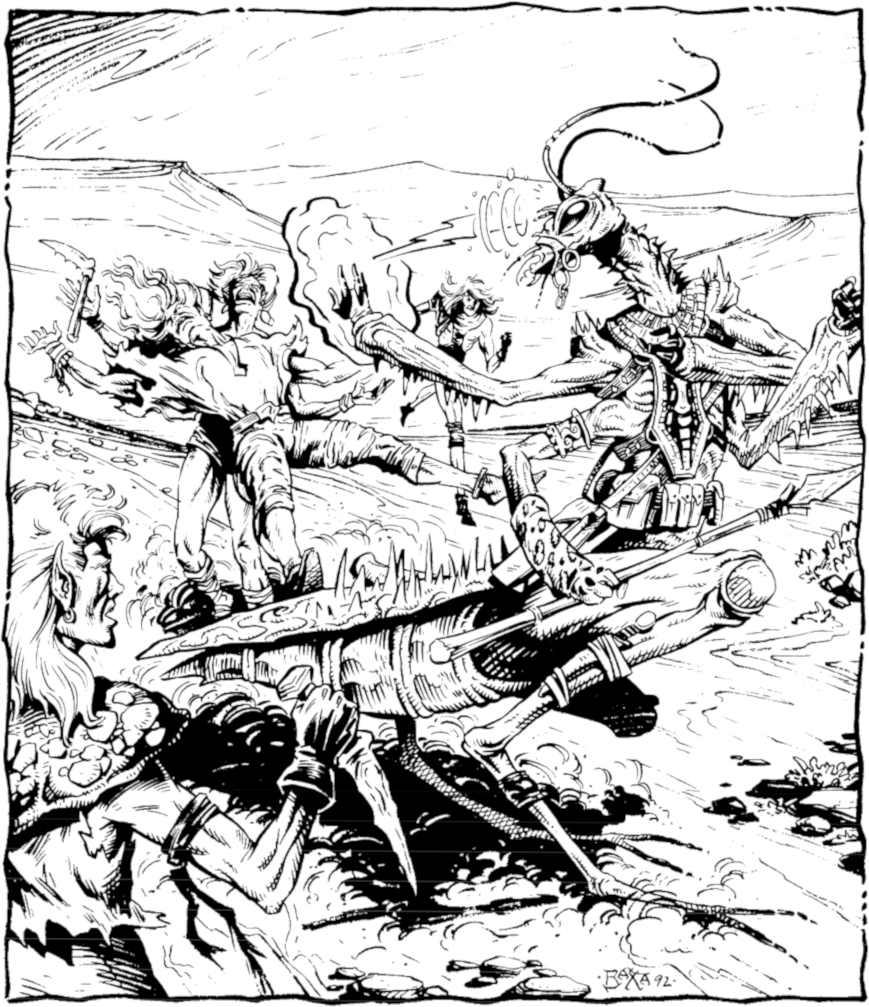
\includegraphics[width=\textwidth-1cm]{images/psywarrior-1.png}
\end{figure*}

\subsection{Making a Psychic Warrior}
Despite his spectacular combat powers, a psychic warrior is not a typical front-line combatant. Although a fighter, barbarian, or gladiator might swing a sword more accurately, or with greater force, a psychic warrior depends on his repertoire of power and feats. A psychic warrior is the psionic equivalent of an eldritch knight or a warmage from other settings. A psychic warrior's role in the party isn't easily defined, but his combination of physical might, the Way, and martial arts is useful in almost any encounter.

\textbf{Races:} Practicing psionics as part of hunting or combat comes as naturally to a Thri-kreen, as running comes to an elf. The Thri-kreen propensity to become ``chakak'' is rooted in the kreen ancestral memory. Becoming ``chakak'' is an almost unavoidable rite of kreen adulthood. Even kreen who focus their attentions in another class, such as the druid, tend to take at least one level as a psychic warrior. Nearly all pack-leaders and clutchleaders are accomplished chakak. Because of the clutch-mind, kreen chakak are far more cooperative, and infinitely less competitive with each other than the psychic warriors of other races.

Muls particularly excel as psychic warriors, as do humans, elves, and dwarves, to a lesser extent. Aarakocra and pterran psychic warriors are rare in those racial cultures, but individuals who take up the psychic warrior class tend to thrive. Halflings and jozhal psychic warriors are virtually unheard of.

\textbf{Alignment:} Psychic warriors tend towards neutrality with regards to good and evil, but they must be either lawful or chaotic. Chaotic psychic warriors, known commonly as ``mercenary psionicists,'' often work asattack thugs or assassins, though like bards, mercenary psionicists are notorious for switching allegiances according to the highest purse. Lawful psychic warriors, or ``mindguards,'' are the most sought-after personal guards for nobles and merchant lords. Like the elite rogue servants of the nobles, mindguards serve loyally in exchange for lavish compensation.

\subsection{Game Rule Information}

\textbf{Alignment:} Any lawful or chaotic.

\textbf{Hit Die:} d8.

\subsubsection{Class Skills}
\skill{Autohypnosis} (Wis), \skill{Climb} (Str), \skill{Concentration} (Con), \skill{Craft} (Int), \skill{Intimidate} (Cha), \skill{Jump} (Str), \skill{Knowledge} (psionics) (Int), \skill{Profession} (Wis), \skill{Ride} (Dex), and \skill{Search} (Int).

\textbf{Skill Points per Level:} 2 + Int modifier ($\times 4$ at 1st level).

\subsubsection{Class Features}

\textbf{Weapon and Armor Proficiency:} Psychic warriors are proficient with all simple and martial weapons, with all types of armor (heavy, medium, and light), and with shields (except tower shields).

\textbf{Power Points/Day:} A psychic warrior's ability to manifest powers is limited by the power points he has available. His base daily allotment of power points is given on \tabref{The Psychic Warrior}. In addition, he receives bonus power points per day if he has a high Wisdom score (see \tabref{Ability Scores and Bonus Power Points}). His race may also provide bonus power points per day, as may certain feats and items. A 1st-level psychic warrior gains no power points for his class level, but he gains bonus power points (if he is entitled to any), and can manifest the single power he knows with those power points.

\textbf{Powers Known:} A psychic warrior begins play knowing one psychic warrior power of your choice. Each time he achieves a new level, he unlocks the knowledge of a new power.

Choose the powers known from the psychic warrior power list. (Exception: The feat \feat{Expanded Knowledge} do allow a psychic warrior to learn powers from the lists of other classes.) A psychic warrior can manifest any power that has a power point cost equal to or lower than his manifester level.

The total number of powers a psychic warrior can manifest in a day is limited only by his daily power points.

A psychic warrior simply knows his powers; they are ingrained in his mind. He does not need to prepare them (in the way that some spellcasters prepare their spells), though he must get a good night's sleep each day to regain all his spent power points.

The Difficulty Class for saving throws against psychic warrior powers is 10 + the power's level + the psychic warrior's Wisdom modifier.

\textbf{Maximum Power Level Known:} A psychic warrior begins play with the ability to learn 1st-level powers. As he attains higher levels, he may gain the ability to master more complex powers.

To learn or manifest a power, a psychic warrior must have a Wisdom score of at least 10 + the power's level.

\textbf{Bonus Feats:} At 1st level, a psychic warrior gets a bonus combat-oriented feat in addition to the feat that any 1st level character gets and the bonus feat granted to a human character. The psychic warrior gains an additional bonus feat at 2nd level and every three levels thereafter (5th, 8th, 11th, 14th, 17th, and 20th). These bonus feats must be drawn from the feats noted as fighter bonus feats or psionic feats. The psychic warrior must still meet all prerequisites for the bonus feat, including ability score and base attack bonus minimums as well as class requirements. A psychic warrior cannot choose feats that specifically require levels in the fighter class unless he is a multiclass character with the requisite levels in the fighter class.

These bonus feats are in addition to the feats that a character of any class gains every three levels. A psychic warrior is not limited to fighter bonus feats and psionic feats when choosing these other feats.

\subsubsection{Ex-Psychic Warriors}
Any psychic warrior who ceases to be either lawful or chaotic, can no longer progress as a psychic warrior. She keeps all her powers known, power points, and bonus feats.

\subsection{Playing a Psychic Warrior}
When you mold your body and mind with the same rigor as a dwarf tempers his steel, no feat or combat prowess is beyond you. Through it all, you seek to understand the secret knowledge of combat, and how to take your nexus---a point in the center of your being where physical, mental, and spiritual energy can be harnessed---to the next level. You know the exact extent of your abilities and how hard it was to achieve them, so you are prone to showing it off flamboyantly, and claim to fear nothing.

Psychic warriors adventure for a plethora of reasons. Neither the religious fervor of an elemental cleric nor the glory of the fighter causes you to travel the Tablelands. More than faith, more than glory, you seek martial perfection. Whether you find that perfection in the cannibal-filled jungles of the Forest Ridge, in the choking silt of the Silt Sea, or in the den of the deadly braxat, you are driven to learn it and master it.

\subsubsection{Religion}
Religion might be entirely delusional to you, or you might find comfort in the elemental (or paraelemental) faiths, or even in the sorcerer-monarch of your city-state. If you are among the minority of psychic warriors who revere an element, you probably worship one associated with physical strength, such as Earth or Magma, or wisdom, such as Air or Sun.

\subsubsection{Other Classes}
Psychic warriors get along best with rogues, and to a lesser extent, fighters and bards. Generally, allies who show admiration for the psychic warriors' talents tend to get along well with the psychic warrior. Gladiators tend to get suspicious and envious of the psychic warrior's shows of unnatural and spectacular force, and many psychic warriors take a perverse pleasure in playing against the gladiator's jealousy, showing up the gladiator with spectacular stunts. Psychic warriors pretend to be indifferent to wizards, and to a lesser extent, psions, but many secretly envy the spectacle of a fireball.

\subsubsection{Combat}

You use your sword skills to defeat your foes as well as the limited access to manifest melee-oriented psionic powers. You have access to an amazing array of powerful combat feats. You have almost exclusive access to feats such as Deep Impact, Focused Sunder, and Wounding Attack, and you would do well to learn at least some of them. You have a limited selection of powers, so choose them carefully so you have a good mix of offensive, defensive and utility powers at your disposal.

\subsubsection{Advancement}
Your training began when you fought your way into an apprenticeship with a mentor---either a retired psychic warrior or an instructor in one of the many psionic academies dotting the Tablelands. You knew that finding that psychic warrior apprenticeship would not be that easy---that in fact, it would be an ordeal designed to test your body and mind to its fullest.

As a psychic warrior, your selection of psionic powers is paramount to your success. You might choose to focus on a specific psionic discipline, such as psychometabolism or psychokinesis, but learning a few powers from other disciplines is almost always advisable. True success in combat requires being ready for everything.

\subsection{Starting Packages}
\subsubsection{The Defender}

Mul Psychic Warrior

\textbf{Ability Scores:} Str 18, Dex 12, Con 15, Int 10, Wis 15, Cha 6.

\textbf{Skills:} \skill{Autohypnosis}, \skill{Concentration}, \skill{Intimidate}.

\textbf{Languages:} Common.

\textbf{Feat:} \feat{Combat Manifestation}.

\textbf{Weapons:} Great macahuitl (2d6/19--20)

Five javelins (1d6, 9 m).

\textbf{Armor:} Scale mail (+4 AC).

\textbf{Other Gear:} Standard adventurer's kit, 45 cp.

\subsubsection{The Destroyer}

Thri-kreen Psychic Warrior

\textbf{Ability Scores:} Str 17, Dex 17, Con 12, Int 8, Wis 16, Cha 4.

\textbf{Skills:} \skill{Concentration}, \skill{Intimidate}, \skill{Jump}.

\textbf{Languages:} Kreen.

\textbf{Feat:} \feat{Multiweapon Fighting}.

\textbf{Weapons:} Gythka (1d8/1d8)

Four chatkchas (1d6, 6 m).

\textbf{Armor:} Leather (+2 AC).

\textbf{Other Gear:} Standard adventurer's kit.

\subsubsection{The Skirmisher}

Human Psychic Warrior

\textbf{Ability Scores:} Str 14, Dex 13, Con 12, Int 10, Wis 15, Cha 8.

\textbf{Skills:} \skill{Concentration}, \skill{Intimidate}, \skill{Jump}, \skill{Psicraft}, \skill{Spot} (cc).

\textbf{Languages:} Common.

\textbf{Feat:} \feat{Dodge}, \feat{Weapon Focus} (glaive).

\textbf{Weapons:} Gouge (1d10/$\times$3)

Five javelins (1d6, 9 m).

\textbf{Armor:} Studded leather (+3 AC).

\textbf{Other Gear:} Standard adventurer's kit, 100 cp.

\subsection{Psychic Warriors on Athas}
\Quote{'Your studies have gone well, Turek,' he said quietly. 'You have learned the basics of psychic defense. It is time to practice your lessons.'

Turek nodded, his palms wet with sweat. He had known this was coming; he was one of the older students and it was time to begin his final studies before leaving the academy.

His master watched him without expression. Suddenly Turek found his attention ripped away from the patio and the master's physical form, being drawn inward. In his mind's eye a glowing sword appeared, poised to strike. 'I am the Sword', his master whispered. I pierce barriers and rend armor.' Turek swallowed nervously and summoned his defense. 'I am the Void, he thought over and over again. I cannot be found, I cannot be harmed.'

The Sword lunged forward, driving through the heart of the nothingness that cloaked Turek's presence...}{}

No place on Athas is safe from psionics. Armies and fortresses mean nothing to a master of the Way. To answer the threat of psionic attack, nobles and merchants retain the services of mercenary psionicists to guard against other users of the Way.

With a potential to advance in a number of different directions---offensive, defensive, support, and quick strike---psychic warriors make excellent additions to adventuring parties.

\subsubsection{Daily Life}

A psychic warrior spends the majority of his time perfecting his mind and body. The mental and spiritual demands of the Way require constant attention, so he can spare little time for carousing.

A psychic warrior with an apprentice spends much of his time training his student. A psychic warrior without one might or might not spend time seeking out one, according to his whims.

\subsubsection{Notables}

Hurgen Vurst, the half-giant garrison chief for Fort Harbeth is considered to be one of the most deadly specimens of his race, combining massive strength and a cleverness rarely found on half-giants. Chukaka the thri-kreen, was one of the first to be coin the term Kiltektet (the-learning-pack-who-enlightens), was a psychic warrior. Known as much for her wisdom, her teachings, as for her chatkchas, she is regarded by many the prototypical psychic warrior---serene, poised, and deadly.

\subsubsection{Organizations}

There is no specific organization that caters to psychic warriors. The Exalted Path (for males) and Serene Bliss (for females) orders in the city-state of Nibenay keep the city's ancient monastic tradition and they usually have several psychic warriors in their milieu. Villichi communities, female humans born with amazing psionic abilities, lie hidden in the deserts, harboring powerful psychic warriors.

\subsubsection{NPC Reactions}

As with fighters, individuals react to psychic warriors based on their previous interactions with other members of the class.

Gladiators have mixed feelings towards psychic warriors, they abilities can be of great value in the arena, but sometimes they feel a bit jealous of those abilities themselves, and they do not like other show offs competing for attention during gladiatorial matches. The only characters that psychic warriors as a rule will have an extremely hard time getting along with are other psychic warriors. Any party unfortunate enough to include more than one psychic warrior will be wrought with petty bickering, snide remarks, and endless competitions of spectacular force.

Merchants and nobles, on the other hand, greatly appreciate psychic warriors. They can always find ready employment as an elite mercenary, in the permanent guard of a noble family, or a merchant house sentry cadre.

\subsubsection{Psychic Warrior Lore}

Characters with ranks in \skill{Knowledge} (psionics) can research psychic warriors to learn more about them. When a character makes a skill check, read or paraphrase the following, including the information from lower DCs.

\textbf{DC 10:} A psychic warrior is a psionic sword-swinger who thinks he knows more about swordplay than anyone else.

\textbf{DC 15:} Like psions and wilders, psychic warrior walk the Unseen Way. Unlike them, psychic warriors train their bodies with the same rigor that they train their minds.

\textbf{DC 20:} Psychic warriors are strong, calm, and lethal. They gain the most psychic might of all those who study the Way.

\Class{Ranger}
{What you call monsters and beasts are simply other beings trying to survive in the wastelands. Some of them are just as desperate, lost, and confused as you are.}{Sudatu, elven scout}

The wastes of Athas are home to fierce and cunning creatures, from the bloodthirsty tembo to the malicious gaj. Because of that, Athasians have long learned how to adapt and survive even in the most inhospitable and savage environments.

One of the most cunning and powerful creatures of the wastes is the ranger, a skilled hunter and stalker. He knows his lands as if they were his home (as indeed they are); he knows his prey in deadly detail.

\HalfSpellcasterTable{The Ranger}{
1 & +1 & +2 & +2 & +0 & 1st favored enemy, Track, wild empathy &&&&\\
2 & +2 & +3 & +3 & +0 & Combat style &&&&\\
3 & +3 & +3 & +3 & +1 & Endurance &&&&\\
4 & +4 & +4 & +4 & +1 & Animal companion & 0 &&&\\
5 & +5 & +4 & +4 & +1 & 2nd favored enemy & 0 &&&\\
6 & +6/+1 & +5 & +5 & +2 & Improved combat style & 1 &&&\\
7 & +7/+2 & +5 & +5 & +2 & Woodland stride & 1 &&&\\
8 & +8/+3 & +6 & +6 & +2 & Swift tracker & 1 & 0 &&\\
9 & +9/+4 & +6 & +6 & +3 & Evasion & 1 & 0 &&\\
10 & +10/+5 & +7 & +7 & +3 & 3rd favored enemy & 1 & 1 &&\\
11 & +11/+6/+1 & +7 & +7 & +3 & Combat style mastery & 1 & 1 & 0 &\\
12 & +12/+7/+2 & +8 & +8 & +4 & & 1 & 1 & 1 &\\
13 & +13/+8/+3 & +8 & +8 & +4 & Camouflage & 1 & 1 & 1 &\\
14 & +14/+9/+4 & +9 & +9 & +4 & & 2 & 1 & 1 & 0 \\
15 & +15/+10/+5 & +9 & +9 & +5 & 4th favored enemy & 2 & 1 & 1 & 1 \\
16 & +16/+11/+6/+1 & +10 & +10 & +5 & & 2 & 2 & 1 & 1 \\
17 & +17/+12/+7/+2 & +10 & +10 & +5 & Hide in plain sight & 2 & 2 & 2 & 1 \\
18 & +18/+13/+8/+3 & +11 & +11 & +6 & & 3 & 2 & 2 & 1 \\
19 & +19/+14/+9/+4 & +11 & +11 & +6 & & 3 & 3 & 3 & 2 \\
20 & +20/+15/+10/+5 & +12 & +12 & +6 & 5th favored enemy & 3 & 3 & 3 & 3}


\subsection{Making a Ranger}
Rangers are capable in combat, although less so in open melee than the fighter, gladiator, or barbarian. His skills allow him to survive in the wilderness, to find his prey and to avoid detection. The ranger has the ability to gain special knowledge of certain types of creatures or lands. Knowledge of his enemies makes him more capable of finding and defeating those foes. Knowledge of terrain types or of specific favored lands makes it easier for him to live off the land, and makes it easier for him to take advantage of less knowledgeable foes. Rangers eventually learn to use the lesser spirits that inhabit Athas in order to produce spell-like effects. These lesser spirits inhabit small features of the land -- rocks, trees, cacti and the like.

These spirits are relatively powerless, and cannot manifest themselves. Their awareness is low, and their instincts are of the most primitive sort. The relationship between these lesser spirits and the creatures known as Spirits of the Land is unknown.

\textbf{Races:} As the race that carries the most fear and hatred of other races, and as the people with the richest land to protect, Halflings become rangers more commonly than any other race except for half-elves. Halflings are at home in their terrain (typically Forest Ridge or the Jagged Cliffs) and the ranger class teaches them the grace to move without detection, often to deadly effect. Their practice of cannibalism to emphasize their superiority over other sentient beings puts the ranger's tracking abilities to deadly use. Halfling rangers tend to take favored lands primarily, followed by favored enemy benefits. In the Forest Ridge, halfling rangers tend to pick pterrans and other neighboring races as favored enemies; rangers of the Jagged Cliffs tend to focus on bvanen, and kreen.

Elves frequently become rangers, serving as scouts and hunters for their tribes, but elves are not as naturally drawn to the wilderness as they are to magic. Half-elves are the race most compellingly drawn to the ranger class, since their isolation and natural gift with animals gives them a head start above rangers of other races. Half-Elven rangers sometimes seek to impress their Elven cousins with their desert skills, and when they are rejected, the wilderness often becomes the half-elf's only solace. A few half-elves turn to bitter hatred of the parent races that rejected them, and become merciless slave--hunters.

Although ranger skills do not come to naturally humans, their famous adaptability wins out in the end, and many humans make fine rangers. A few muls take up the ranger class while surviving in the wilderness after escaping slavery. Dwarves who become rangers find that their focus ability combines powerfully with the abilities of favored enemy and favored lands, but such characters rarely become adventurers since they tend to master wilderness skills in order to guard Dwarven communities.

Pterran rangers are common since rangers get along so well with the druidic and psionic leaders of the pterran villages. Aarakocra are similarly drawn to the ranger class to protect their villages from predators and enemies. Rangers are not unusual among the most hated humanoid races of Athas, such as gith, belgoi, and braxat. Among the various and dwindling communities of the wastes rangers are the most common character class.

\textbf{Alignment:} Rangers can be of any alignment, although they tend not to be lawful, preferring nature to civilization, silence to casual conversation, and ambush to meeting a foe boldly on the battlefield. Good rangers often serve as protectors of a village or of a wild area. In this capacity, rangers try to exterminate or drive off evil creatures that threaten the rangers' lands. Good rangers sometimes protect those who travel through the wilderness, serving sometimes as paid guides, but sometimes as unseen guardians. Neutral rangers tend to be wanderers and mercenaries, rarely tying themselves down to favored lands. The tracking and animal skills of rangers are well known in the World; virtually every trade caravan has at least one ranger scout or mekillot handler. Sometimes they stalk the land for vengeance, either for themselves or for an employer. Generally only evil rangers ply their skills in the slave trade. Other evil rangers seek to emulate nature's most fearsome predators, and take pride and pleasure in the terror that strangers take in their names.

\subsection{Game Rule Information}

\textbf{Hit Die:} d8.

\subsubsection{Class Skills}
\skill{Climb} (Str), \skill{Concentration} (Con), \skill{Craft} (Int), \skill{Handle Animal} (Cha), \skill{Heal} (Wis), \skill{Hide} (Dex), \skill{Jump} (Str), \skill{Knowledge} (dungeoneering) (Int), \skill{Knowledge} (geography) (Int), \skill{Knowledge} (nature) (Int), \skill{Listen} (Wis), \skill{Move Silently} (Dex), \skill{Profession} (Wis), \skill{Ride} (Dex), \skill{Search} (Int), \skill{Spot} (Wis), \skill{Survival} (Wis), and \skill{Use Rope} (Dex).

\textbf{Skill Points per Level:} 6 + Int modifier ($\times 4$ at 1st level).

\begin{figure*}[b!]
\centering
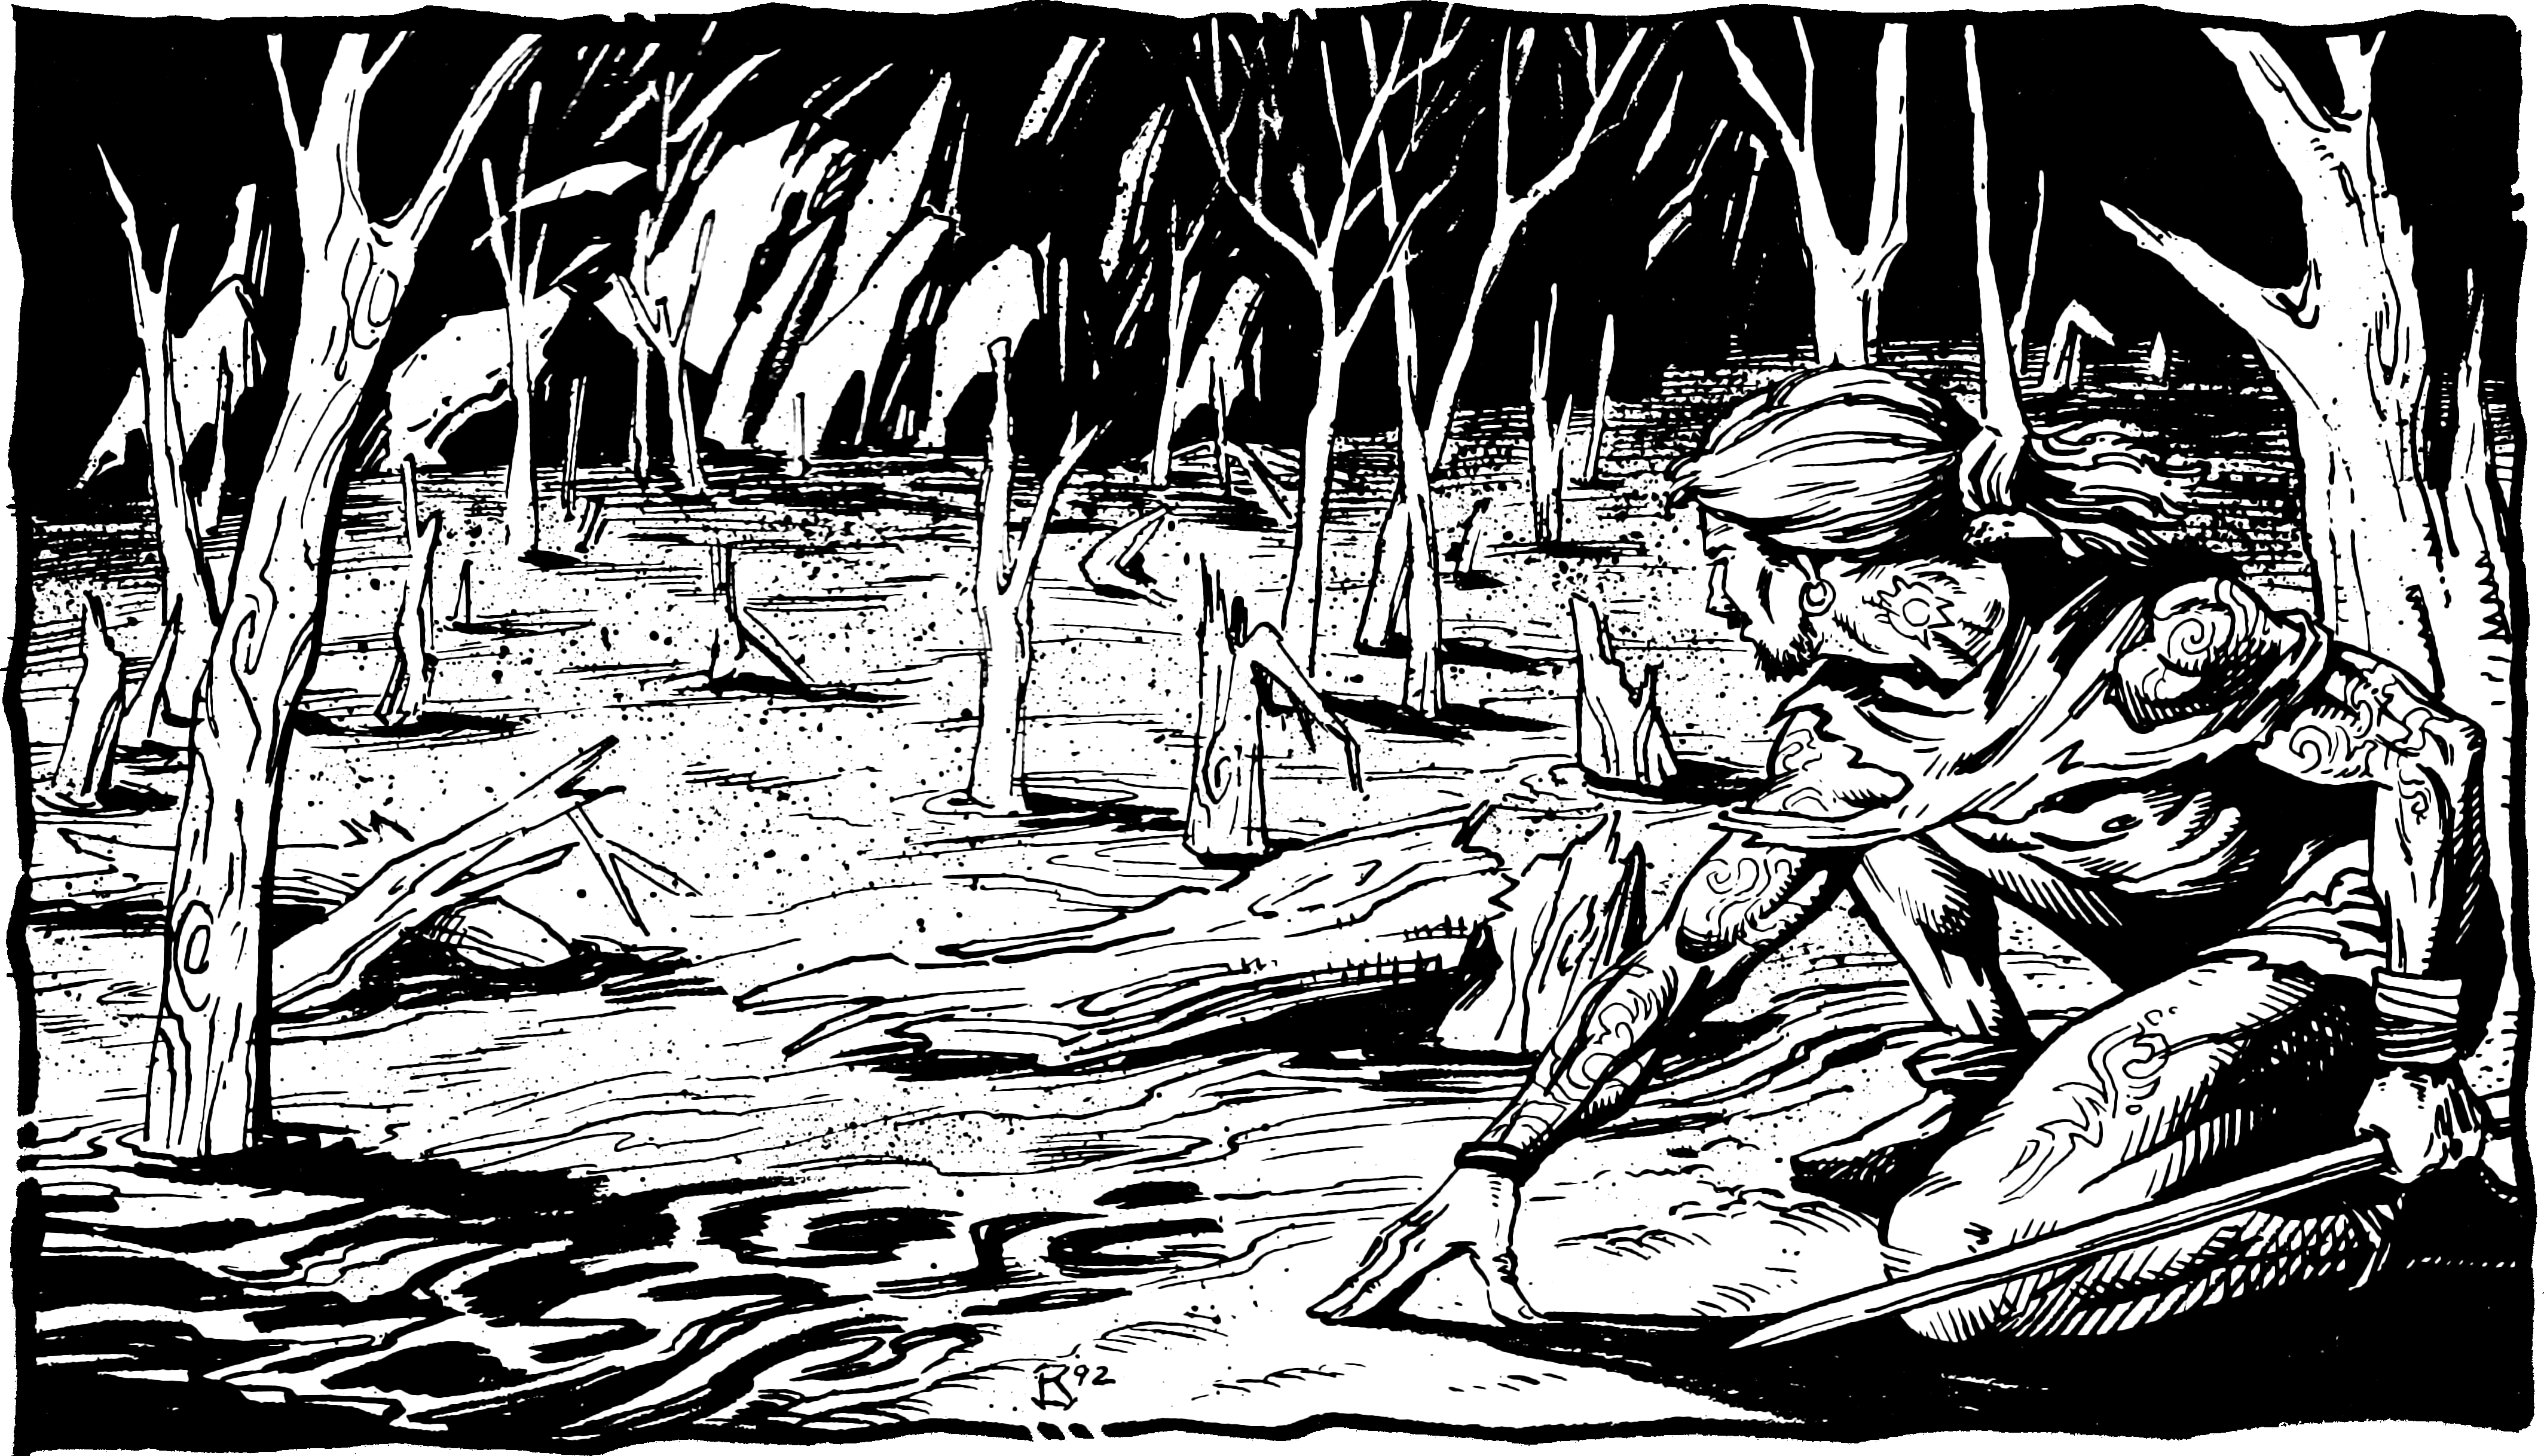
\includegraphics[width=\textwidth]{images/ranger-2.png}
\par\textit{\small\textcopyright Wizards of the Coast, 2020.}
\end{figure*}

\subsubsection{Class Features}
\textbf{Weapon and Armor Proficiency:} A ranger is proficient with all simple and martial weapons, and with light armor and shields (except tower shields).

\textbf{Favored Enemy (Ex):} At 1st level, a ranger may select a type of creature from among those given on \tabref{Athasian Favored Enemies}. The ranger gains a +2 bonus on \skill{Bluff}, \skill{Listen}, \skill{Sense Motive}, \skill{Spot}, and \skill{Survival} checks when using these skills against creatures of this type. Likewise, he gets a +2 bonus on weapon damage rolls against such creatures.

At 5th level and every five levels thereafter (10th, 15th, and 20th level), the ranger may select an additional favored enemy from those given on the table. In addition, at each such interval, the bonus against any one favored enemy (including the one just selected, if so desired) increases by 2.

If the ranger chooses humanoids or outsiders as a favored enemy, he must also choose an associated subtype, as indicated on the table. If a specific creature falls into more than one category of favored enemy, the ranger's bonuses do not stack; he simply uses whichever bonus is higher.

\Table{Athasian Favored Enemies}{X X}{
\tableheader Type (Subtype) & \tableheader Example\\
Aberration & gaj \\
Animal & lion \\
Construct & golem \\
Elemental (air) & air elemental beast \\
Elemental (earth) & crystal spider \\
Elemental (fire) & fire incarnation \\
Elemental (water) & rain paraelemental beast \\
Giant & beasthead giant \\
Humanoid (dwarf) & dwarf \\
Humanoid (elf) & elf \\
Humanoid (gith) & gith \\
Humanoid (halfling) & halfling \\
Humanoid (human) & human \\
Humanoid (jozhal) & jozhal \\
Humanoid (nikaal) & nikaal \\
Humanoid (psionic) & villichi \\
Humanoid (pterran) & pterran \\
Humanoid (reptilian) & silt runner \\
Humanoid (tarek) & tarek \\
Humanoid (tari) & tari \\
Magical beast & kirre \\
Monstrous humanoid & Thri-kreen \\
Outsider & silt half-elemental \\
Plant & hunting cactus \\
Undead & kaisharga \\
Vermin & kank}

\Table{Athasian Terrains}{X X}{
\tableheader Terrain Type & \tableheader Terrain Type\\
Boulder Field & Rocky Badland \\
Forest & Salt Flat \\
Jagged Cliffs & Sandy Waste \\
Mountain & Sea of Silt \\
Mud Flat & Stony Barren \\
Obsidian Waste & Swamp \\
Ocean & Verdant Belt}

\textbf{Favored Terrain (Ex):} At any time when a ranger could normally select a favored enemy, he may instead choose to select a favored terrain given on \tabref{Athasian Terrains}. A ranger receives a +2 bonus on \skill{Hide}, \skill{Listen}, \skill{Move Silently}, \skill{Search}, \skill{Spot} and \skill{Survival} checks made within your favored terrain. Likewise, he gets +2 bonus on \skill{Knowledge} (geography) and \skill{Knowledge} (nature) checks about your favored terrain.

This ability uses the same graduated progression that the favored enemy ability receives.

For example, at first level Sudatu selects monstrous humanoids as a favored enemy, receiving a +2 bonus when combating them. At fifth level, instead of taking a new favored enemy, he selects a Rocky Badlands as his favored terrain, and chooses to increase his favored enemy bonus to +4. At 10th level, Sudatu may again choose a new Favored Enemy, and may also choose between raising his favored enemy or favored terrain bonus by +2.

\textbf{Track:} A ranger gains \feat{Track} as a bonus feat.

\textbf{Wild Empathy (Ex):} A ranger can improve the attitude of an animal. This ability functions just like a \skill{Diplomacy} check to improve the attitude of a person. The ranger rolls 1d20 and adds his ranger level and his Charisma modifier to determine the wild empathy check result. The typical domestic animal has a starting attitude of indifferent, while wild animals are usually unfriendly.

To use wild empathy, the ranger and the animal must be able to study each other, which means that they must be within 9 meters of one another under normal visibility conditions. Generally, influencing an animal in this way takes 1 minute, but, as with influencing people, it might take more or less time.

The ranger can also use this ability to influence a magical beast with an Intelligence score of 1 or 2, but he takes a $-4$ penalty on the check.

\textbf{Combat Style (Ex):} At 2nd level, a ranger must select one of two combat styles to pursue: archery or two-weapon combat. This choice affects the character's class features but does not restrict his selection of feats or special abilities in any way.

If the ranger selects archery, he is treated as having the \feat{Rapid Shot} feat, even if he does not have the normal prerequisites for that feat.

If the ranger selects two-weapon combat, he is treated as having the \feat{Two-Weapon Fighting} feat, even if he does not have the normal prerequisites for that feat.

The benefits of the ranger's chosen style apply only when he wears light or no armor. He loses all benefits of his combat style when wearing medium or heavy armor.

\textbf{Endurance:} A ranger gains \feat{Endurance} as a bonus feat at 3rd level.

\textbf{Animal Companion (Ex):} At 4th level, a ranger gains an animal companion selected from the following list: badger, camel, dire rat, dog, riding dog, eagle, hawk, horse (light or heavy), owl, pony, snake (Small or Medium viper), or wolf. If the campaign takes place wholly or partly in an aquatic environment, the following creatures may be added to the ranger's list of options: manta ray, porpoise, Medium shark, and squid. This animal is a loyal companion that accompanies the ranger on his adventures as appropriate for its kind.

This ability functions like the druid ability of the same name, except that the ranger's effective druid level is one-half his ranger level. A ranger may select from the alternative lists of animal companions just as a druid can, though again his effective druid level is half his ranger level. Like a druid, a ranger cannot select an alternative animal if the choice would reduce his effective druid level below 1st.

\textbf{Spells:} Beginning at 4th level, a ranger gains the ability to cast a small number of divine spells, which are drawn from the ranger spell list. A ranger must choose and prepare his spells in advance (see below).

To prepare or cast a spell, a ranger must have a Wisdom score equal to at least 10 + the spell level. The Difficulty Class for a saving throw against a ranger's spell is 10 + the spell level + the ranger's Wisdom modifier.

Like other spellcasters, a ranger can cast only a certain number of spells of each spell level per day. His base daily spell allotment is given on \tabref{The Ranger}. In addition, he receives bonus spells per day if he has a high Wisdom score. When \tabref{The Ranger} indicates that the ranger gets 0 spells per day of a given spell level, he gains only the bonus spells he would be entitled to based on his Wisdom score for that spell level. The ranger does not have access to any domain spells or granted powers, as a cleric does.

A ranger prepares and casts spells the way a cleric does, though he cannot lose a prepared spell to cast a cure spell in its place. A ranger may prepare and cast any spell on the ranger spell list, provided that he can cast spells of that level, but he must choose which spells to prepare during his daily meditation.

Through 3rd level, a ranger has no caster level. At 4th level and higher, his caster level is one-half his ranger level.

\textbf{Improved Combat Style (Ex):} At 6th level, a ranger's aptitude in his chosen combat style (archery or two-weapon combat) improves. If he selected archery at 2nd level, he is treated as having the \feat{Manyshot} feat, even if he does not have the normal prerequisites for that feat.

If the ranger selected two-weapon combat at 2nd level, he is treated as having the \feat{Improved Two-Weapon Fighting} feat, even if he does not have the normal prerequisites for that feat.

As before, the benefits of the ranger's chosen style apply only when he wears light or no armor. He loses all benefits of his combat style when wearing medium or heavy armor.

\textbf{Woodland Stride (Ex):} Starting at 7th level, a ranger may move through any sort of undergrowth (such as natural thorns, briars, overgrown areas, and similar terrain) at his normal speed and without taking damage or suffering any other impairment.

However, thorns, briars, and overgrown areas that are enchanted or magically manipulated to impede motion still affect him.

\textbf{Swift Tracker (Ex):} Beginning at 8th level, a ranger can move at his normal speed while following tracks without taking the normal $-5$ penalty. He takes only a $-10$ penalty (instead of the normal $-20$) when moving at up to twice normal speed while tracking.

\textbf{Evasion (Ex):} At 9th level, a ranger can avoid even magical and unusual attacks with great agility. If he makes a successful Reflex saving throw against an attack that normally deals half damage on a successful save, he instead takes no damage. Evasion can be used only if the ranger is wearing light armor or no armor. A helpless ranger does not gain the benefit of evasion.

\textbf{Combat Style Mastery (Ex):} At 11th level, a ranger's aptitude in his chosen combat style (archery or two-weapon combat) improves again. If he selected archery at 2nd level, he is treated as having the \feat{Improved Precise Shot} feat, even if he does not have the normal prerequisites for that feat.

If the ranger selected two-weapon combat at 2nd level, he is treated as having the \feat{Greater Two-Weapon Fighting} feat, even if he does not have the normal prerequisites for that feat.

As before, the benefits of the ranger's chosen style apply only when he wears light or no armor. He loses all benefits of his combat style when wearing medium or heavy armor.

\textbf{Camouflage (Ex):} A ranger of 13th level or higher can use the \skill{Hide} skill in any sort of natural terrain, even if the terrain doesn't grant cover or concealment.

\textbf{Hide in Plain Sight (Ex):} While in any sort of natural terrain, a ranger of 17th level or higher can use the \skill{Hide} skill even while being observed.

\subsection{Playing a Ranger}

As a ranger, you nurture a close, almost mystical connection to the deadly terrain of Athas. To you, the burnt landscape is not a friend, but a well-respected adversary. Danger is always present, yet you understand it and even find a certain succor in living alongside it.

\subsubsection{Religion}

Many rangers pay homage to the elements, but a greater number honor the moons and the stars that guide them in the night---even though these celestial bodies do not have priests. In several city-states, particularly Gulg,
Kurn, and Eldaarich, many rangers owe fealty to the sorcerer-kings---virtually the entire noble caste of Gulg is comprised of rangers called judaga. Some rangers pay patronage to the Spirits of the Land, although these spirits do not bestow spells on rangers except those that multi-class as druid.

\subsubsection{Other Classes}

Rangers are slow to make friends with anyone, but have a particular affinity to druids, and to a lesser extent, barbarians and psions. Rangers tend not to lean on others for support and friendship, and often find it difficult to tolerate others who are quite different from themselves, such as talkative traders or controlling templars. Good rangers might simply try to avoid sharing a watch with a character that annoys them; neutral rangers tend to abandon annoying companions or just let them die; while evil rangers act friendly to the annoying companion and then slit their throat in their sleep.

Good rangers tend to hate defilers, although many rangers are ignorant of the distinction between preserving and defiling and hate wizards of all stripes. Strangely, many rangers have little objection to taking a companion who is of a favored enemy race, so long as that they are convinced that the companion is trustworthy and loyal.

\subsubsection{Combat}

Although you are a formidable warrior, you usually prefer not to stand against the sheer might of Athas' fighter, barbarians and gladiators. Your greatest ally is the environment itself. While in you favored terrain, you have a clear advantage over your adversaries. Try choosing favored enemies that are more common in your favored terrain.

As you advance, you are well served to invest in spells that have an effect other than dealing damage. If you can't drop a foe in one or two attacks, you can use entangle, snare, sting of the gold scorpion, or the like to make your opponents less dangerous in a prolonged fight.

\subsubsection{Advancement}

Perhaps the most dangerous place in Athas is inside a city-state: an environment rife with political intrigue, diseases, and assassination. To escape these noxious environs, you sought refuge in the wild where even the foulest elements of a society fear to tread. By gaining an intimate knowledge of this hazardous realm, you buy some breathing room and security from the urban madness.

As your ranger abilities increase, you find the Athasian wilderness a more and more inviting place (if a place with such constant peril can be called inviting). You can use your skills to establish safe havens for yourself or to gain employment opportunities---perhaps guiding a group of recently caught slaves through the Tyr valley or some noble into distant dangerous, location. You can also find that continuing to advance as a ranger or barbarian augments your already impressive abilities in the Athasian lands.

Continue to focus on skills such as Hive, Move Silently, and Survival. Spend discovered treasure on poison, magic weapons, and protective magic. The Mobility feat is good to consider, as is Nature's Child or Wastelander.

\subsection{Starting Packages}
\subsubsection{The Archer}
Elf Ranger

\textbf{Ability Scores:} Str 14, Dex 17, Con 10, Int 10, Wis 13, Cha 8.

\textbf{Skills:} \skill{Hide}, \skill{Listen}, \skill{Move Silently}, \skill{Spot}, \skill{Survival}.

\textbf{Languages:} Common, Elven.

\textbf{Feat:} \feat{Point Blank Shot}, \feat{Track}.

\textbf{Weapons:} Macahuitl (1d8/19--20)

Longbow with 20 arrows (1d8/$\times$3, 30 m).

\textbf{Armor:} Studded leather (+3 AC).

\textbf{Other Gear:} Standard adventurer's kit, 19 cp.

\subsubsection{The Scout}
Halfling Ranger

\textbf{Ability Scores:} Str 11, Dex 17, Con 12, Int 10, Wis 14, Cha 8.

\textbf{Skills:} \skill{Hide}, \skill{Knowledge} (nature), \skill{Listen}, \skill{Move Silently}, \skill{Spot}, \skill{Survival}.

\textbf{Languages:} Halfling.

\textbf{Feat:} \feat{Stealthy}, \feat{Track}.

\textbf{Weapons:} Macahuitl (1d6/19--20)

Small macahuitl (1d3/19--20)

Five javelins (1d4, 9 m).

\textbf{Armor:} Studded leather (+3 AC).

\textbf{Other Gear:} Standard adventurer's kit, 65 cp.

\subsubsection{The Wastelander}
Thri-kreen Ranger

\textbf{Ability Scores:} Str 14, Dex 19, Con 14, Int 8, Wis 15, Cha 4.

\textbf{Skills:} \skill{Hide}, \skill{Knowledge} (nature), \skill{Listen}, \skill{Move Silently}, \skill{Spot}, \skill{Survival}.

\textbf{Languages:} Kreen.

\textbf{Feat:} \feat{Track}, \feat{Wastelander}.

\textbf{Weapons:} Gythka (1d8/1d8)

Three chatkchas (1d6, 6 m).

\textbf{Armor:} Studded leather (+3 AC).

\textbf{Other Gear:} Standard adventurer's kit, 5 cp.

\subsection{Rangers on Athas}
\Quote{Trust me. He might not talk a lot and smell funnier than the rest of your men, but there is no other one I would bring along with me around the Great Ivory Plains.}{Waltian Inika, Gulg dune trader}

The Athasian wilderness is harsh and unforgiving, calling for skilled and capable men to master its ways---the ranger answers that challenge, living a rugged life through clever mastery of his surroundings. The ranger has a potent combination of stealth, woodcraft, magic, and fighting skill, making him the master of the wilderness.

\subsubsection{Daily Life}

A ranger adventures to learn about Athas, to protect nature, and to prove his superior hunting skills. Rangers spend their days in contemplation of nature, and tending their animal companions.

The Athasian ranger is a wanderer who hunts down a defiler to avenge himself for having his village destroyed, or a mercenary hunter for both monsters and humanoid creatures, or even a loner who simply prefers the company of animals.

\subsubsection{Notables}

Tales of halfling snipers are among the common Athasian legends. Any traveler to the Forest Ridge should rightfully fear the cannibals that move without a sound and strike without being seen. Thri-kreen are fabled for their rangers, as they are fast-moving relentless natural hunters, and their unarmed combat abilities become even more deadly when applied to subduing a quarry.

\subsubsection{Organizations}

There is no organized ranger organization; you are most likely to be a loner---or at best the leader of a group of raiders or renegades---than you are to gather with other rangers.

Often merchant houses are eager to employ you as a caravan guide through the most dangerous trade routes, or a city-state's templarate might hire you to provide a safe path to a templar patrol.

\subsubsection{NPC Reactions}

Within a city-state or large settlement, you find that you are either ignored or regarded with some small amount of curiosity. It is only after a city-dweller find himself outside the boundaries of his city-state that he truly appreciates you. Indeed, he holds you in the highest of regards, knowing that you are all that stands between him and a horrible death in the wastes.

\subsubsection{Ranger Lore}

Characters with ranks in \skill{Knowledge} (nature) can research rangers to learn more about them. When a character makes a skill check, read or paraphrase the following, including the information from lower DCs.

\textbf{DC 10:} Only those assisted by a ranger can hope to survive in the Athasian wilderness for long.

\textbf{DC 15:} Rangers move with ease through the harsh terrains that others find dangerous or impassable. They make of this aptitude to specialize in battling specific creatures of the wild.

\textbf{DC 20:} As a ranger advances in knowledge and skill, he grows more and more connected to the land, and eventually manages to draw spells from it.

\Class{Rogue}
{Marek, always helpful, said that the UnderTyr catacombs are supposed to be haunted. Think I'll go make some inquiries about where a 'heretic' like me can get some holy earth. Always go prepared...}{Janos, human rogue}

{\tableheader Dark Sun} offers a world of intrigue, manipulation, secret deals, and subtle treachery---in short, a rogue's playground. Rather than eking out their living at the
borders of society, many Athasian rogues dominate the action in many of the most powerful political factions in the Seven Cities: the Noble Houses, the templars, and the Merchant Houses. Often rogues themselves, the wealthy and powerful deploy lesser rogues as pawns in their endless games of acquisition, espionage, and deceit.

Individual rogues run the gamut of Athasian society, from the street rats of the cities to the vagabonds of the outlands, to the prosperous and respectable dune traders, to the low-ranking templars that search their caravans at the gates. Accomplished rogues are often sought by the nobility as agents, and can earn both wealth and honor in such positions---or earn a quick death should they be caught contemplating treachery against their masters.

\WarriorTable{The Rogue}{
1 & +0 & +0 & +2 & +0 & Sneak attack +1d6, trapfinding\\
2 & +1 & +0 & +3 & +0 & Evasion\\
3 & +2 & +1 & +3 & +1 & Sneak attack +2d6, trap sense +1\\
4 & +3 & +1 & +4 & +1 & Uncanny dodge\\
5 & +3 & +1 & +4 & +1 & Sneak attack +3d6\\
6 & +4 & +2 & +5 & +2 & Trap sense +2\\
7 & +5 & +2 & +5 & +2 & Sneak attack +4d6\\
8 & +6/+1 & +2 & +6 & +2 & Improved uncanny dodge\\
9 & +6/+1 & +3 & +6 & +3 & Sneak attack +5d6, trap sense +3\\
10 & +7/+2 & +3 & +7 & +3 & Special ability\\
11 & +8/+3 & +3 & +7 & +3 & Sneak attack +6d6\\
12 & +9/+4 & +4 & +8 & +4 & Trap sense +4\\
13 & +9/+4 & +4 & +8 & +4 & Sneak attack +7d6, special ability\\
14 & +10/+5 & +4 & +9 & +4 & \\
15 & +11/+6/+1 & +5 & +9 & +5 & Sneak attack +8d6, trap sense +5\\
16 & +12/+7/+2 & +5 & +10 & +5 & Special ability\\
17 & +12/+7/+2 & +5 & +10 & +5 & Sneak attack +9d6\\
18 & +13/+8/+3 & +6 & +11 & +6 & Trap sense +6\\
19 & +14/+9/+4 & +6 & +11 & +6 & Sneak attack +10d6, special ability\\
20 & +15/+10/+5 & +6 & +12 & +6 & }

\subsection{Making a Rogue}

A rogue can't stand up face to face with a mul warrior as well as a fighter or gladiator can. With his cunning and your various skills, however, he excels at taking the slightest opportunity and turning to his advantage. His ability to slip under the notice of an observer makes him a capable lone hunter, but his greatest strength are found through interaction with allies and foes, inside or outside, a battle---he can use his enemy`s slightest distraction to deliver a lethal blow, or ensure his party`s safe passage through a templar patrol.

\textbf{Races:} Elves, half-elves, and humans take to the rogue's skills and lifestyle with the greatest ease. Halflings, dwarves, and muls, while not commonly rogues, adapt to the class remarkably well when they take to it. Thri-kreen, pterrans, and aarakocra are usually quite adverse to the rogue class, and tend to do poorly. Half-giant rogues are unheard of except as fictional figures in comical tales around the fireside.

\textbf{Alignment:} Athasian rogues follow opportunity rather than ideals, but as many of them are lawful as chaotic. Lawful rogues tend to seek security and advancement in the service of nobles or in the ranks of the templars.

\subsection{Game Rule Information}
\textbf{Hit Die:} d6.

\subsubsection{Class Skills}
\skill{Appraise} (Int), \skill{Balance} (Dex), \skill{Bluff} (Cha), \skill{Climb} (Str), \skill{Craft} (Int), \skill{Decipher Script} (Int), \skill{Diplomacy} (Cha), \skill{Disable Device} (Int), \skill{Disguise} (Cha), \skill{Escape Artist} (Dex), \skill{Forgery} (Int), \skill{Gather Information} (Cha), \skill{Hide} (Dex), \skill{Intimidate} (Cha), \skill{Jump} (Str), \skill{Knowledge} (local) (Int), \skill{Listen} (Wis), \skill{Move Silently} (Dex), \skill{Open Lock} (Dex), \skill{Perform} (Cha), \skill{Profession} (Wis), \skill{Search} (Int), \skill{Sense Motive} (Wis), \skill{Sleight of Hand} (Dex), \skill{Spot} (Wis), \skill{Tumble} (Dex), \skill{Use Magic Device} (Cha), \skill{Use Psionic Device} (Cha), and \skill{Use Rope} (Dex).

\textbf{Skill Points per Level:} 8 + Int modifier ($\times4$ at 1st level).

\subsubsection{Class Features}
\textbf{Weapon and Armor Proficiency:} Rogues are proficient with all simple weapons, plus the bard's friend, blowgun, garrote, hand crossbow, rapier, sap, shortbow, short sword, small macahuitl, tonfa, widow's knife, and wrist razor. Rogues are proficient with light armor, but not with shields.

\textbf{Sneak Attack:} If a rogue can catch an opponent when he is unable to defend himself effectively from her attack, she can strike a vital spot for extra damage.

The rogue's attack deals extra damage any time her target would be denied a Dexterity bonus to AC (whether the target actually has a Dexterity bonus or not), or when the rogue flanks her target. This extra damage is 1d6 at 1st level, and it increases by 1d6 every two rogue levels thereafter. Should the rogue score a critical hit with a sneak attack, this extra damage is not multiplied.

Ranged attacks can count as sneak attacks only if the target is within 9 meters.

With a sap (blackjack) or an unarmed strike, a rogue can make a sneak attack that deals nonlethal damage instead of lethal damage. She cannot use a weapon that deals lethal damage to deal nonlethal damage in a sneak attack, not even with the usual $-4$ penalty.

A rogue can sneak attack only living creatures with discernible anatomies---undead, constructs, oozes, plants, and incorporeal creatures lack vital areas to attack. Any creature that is immune to critical hits is not vulnerable to sneak attacks. The rogue must be able to see the target well enough to pick out a vital spot and must be able to reach such a spot. A rogue cannot sneak attack while striking a creature with concealment or striking the limbs of a creature whose vitals are beyond reach.

\textbf{Trapfinding:} Rogues (and only rogues) can use the Search skill to locate traps when the task has a Difficulty Class higher than 20.

Finding a nonmagical trap has a DC of at least 20, or higher if it is well hidden. Finding a magic trap has a DC of 25 + the level of the spell used to create it.

Rogues (and only rogues) can use the \skill{Disable Device} skill to disarm magic traps. A magic trap generally has a DC of 25 + the level of the spell used to create it.

A rogue who beats a trap's DC by 10 or more with a \skill{Disable Device} check can study a trap, figure out how it works, and bypass it (with her party) without disarming it.

\textbf{Evasion (Ex):} At 2nd level and higher, a rogue can avoid even magical and unusual attacks with great agility. If she makes a successful Reflex saving throw against an attack that normally deals half damage on a successful save, she instead takes no damage. Evasion can be used only if the rogue is wearing light armor or no armor. A helpless rogue does not gain the benefit of evasion.

\textbf{Trap Sense (Ex):} At 3rd level, a rogue gains an intuitive sense that alerts her to danger from traps, giving her a +1 bonus on Reflex saves made to avoid traps and a +1 dodge bonus to AC against attacks made by traps. These bonuses rise to +2 when the rogue reaches 6th level, to +3 when she reaches 9th level, to +4 when she reaches 12th level, to +5 at 15th, and to +6 at 18th level.

Trap sense bonuses gained from multiple classes stack.

\textbf{Uncanny Dodge (Ex):} Starting at 4th level, a rogue can react to danger before her senses would normally allow her to do so. She retains her Dexterity bonus to AC (if any) even if she is caught flat-footed or struck by an invisible attacker. However, she still loses her Dexterity bonus to AC if immobilized.

If a rogue already has uncanny dodge from a different class she automatically gains improved uncanny dodge instead.

\textbf{Improved Uncanny Dodge (Ex):} A rogue of 8th level or higher can no longer be flanked.

This defense denies another rogue the ability to sneak attack the character by flanking her, unless the attacker has at least four more rogue levels than the target does.

If a character already has uncanny dodge from a second class, the character automatically gains improved uncanny dodge instead, and the levels from the classes that grant uncanny dodge stack to determine the minimum rogue level required to flank the character.

\textbf{Special Abilities:} On attaining 10th level, and at every three levels thereafter (13th, 16th, and 19th), a rogue gains a special ability of her choice from among the following options.

\textit{Crippling Strike (Ex):} A rogue with this ability can sneak attack opponents with such precision that her blows weaken and hamper them. An opponent damaged by one of her sneak attacks also takes 2 points of Strength damage. Ability points lost to damage return on their own at the rate of 1 point per day for each damaged ability.

\textit{Defensive Roll (Ex):} The rogue can roll with a potentially lethal blow to take less damage from it than she otherwise would. Once per day, when she would be reduced to 0 or fewer hit points by damage in combat (from a weapon or other blow, not a spell or special ability), the rogue can attempt to roll with the damage. To use this ability, the rogue must attempt a Reflex saving throw (DC = damage dealt). If the save succeeds, she takes only half damage from the blow; if it fails, she takes full damage. She must be aware of the attack and able to react to it in order to execute her defensive roll---if she is denied her Dexterity bonus to AC, she can't use this ability. Since this effect would not normally allow a character to make a Reflex save for half damage, the rogue's evasion ability does not apply to the defensive roll.

\textit{Dune Trader:} You gain +4 competence bonus to \skill{Diplomacy} checks with regard to buying or selling goods. Furthermore, \skill{Speak Language} becomes a class skill.

\textit{False Vulnerability (Ex):} While lying prone, you are not as helpless as you appear. Opponents do not get +4 to hit you while you are prone, and you can ``kip up,'' or leap from a prone position as a free action. You do not provoke an attack of opportunity when standing up. If this ability is used with a feint action, you get a +4 circumstance bonus to your opposed Bluff roll.

\textit{Improved Evasion (Ex):} This ability works like evasion, except that while the rogue still takes no damage on a successful Reflex saving throw against attacks henceforth she takes only half damage on a failed save. A helpless rogue does not gain the benefit of improved evasion.

\textit{Looter's Luck (Ex):} You can use your \skill{Appraise} skill to instinctively identify the most valuable item in a pile of loot as a move action. The DC for this accomplishment is DC 10 + the number of items in the selection. If you cannot see the items that you are choosing from (e.g. you are trying to pickpocket someone), then a full-round action is required, and the DC rises to 15 + the number of items.

\textit{Notoriety:} The fame of your exploits precedes you in the Seven Cities; you gain +4 to all \skill{Intimidate} and \skill{Bluff} checks. Adventurers seek your fellowship; you receive a +4 to your Leadership score if you have the \feat{Leadership} feat.

\textit{Opportunist (Ex):} Once per round, the rogue can make an attack of opportunity against an opponent who has just been struck for damage in melee by another character. This attack counts as the rogue's attack of opportunity for that round. Even a rogue with the \feat{Combat Reflexes} feat can't use the opportunist ability more than once per round.

\textit{Silver Tongue (Ex):} Your constant dealing with others gives you a keen sense of how to make them believe your lies. You may attempt a retry of the Bluff skill, but with a $-5$ penalty. This ability also gives you a +2 bonus to your \skill{Disguise} skill.

\textit{Skill Mastery:} The rogue becomes so certain in the use of certain skills that she can use them reliably even under adverse conditions.

Upon gaining this ability, she selects a number of skills equal to 3 + her Intelligence modifier. When making a skill check with one of these skills, she may take 10 even if stress and distractions would normally prevent her from doing so. A rogue may gain this special ability multiple times, selecting additional skills for it to apply to each time.

\textit{Slippery Mind (Ex):} This ability represents the rogue's ability to wriggle free from magical effects that would otherwise control or compel her. If a rogue with slippery mind is affected by an enchantment spell or effect and fails her saving throw, she can attempt it again 1 round later at the same DC. She gets only this one extra chance to succeed on her saving throw.

\textit{Feat:} A rogue may gain a bonus feat in place of a special ability.

\subsection{Playing a Rogue}

Rogues run the gamut of society. Athasian rogues range from gutter snipes who prey upon the merchants and free citizens of the cities to vagabonds who steal what they can from passing caravans or merchant trains. At their best, rogues can be in the employ of the nobility, plying their trade by contract in the name of a royal household, or they can be men or women of principle and honor who steal only from the corrupt and wealthy.

There is no thieves' guild on Athasian cities. However, most Athasians rogues attempt to attract a patron. A patron is a noble or senior templar who will sponsor the rogue and protect him under his house and name. The rogue is then expected to perform certain tasks for his new master in return---including theft, spying, and even assassination.

You might adventure because you desire excitement. Someone with your smarts get bored with ordinary pursuits. Alternatively, you might have set off a life of adventure after your big heist or some political manipulation gone wrong. For some reason, you have to keep moving, and a life of adventure offers you a regular change of scenery.

All seek to exercise their abilities to grow to even greater levels of power. You are clever enough to know that there's always more to learn. Although you tend to be (dangerously) self-reliant, you understand the value of having ``friends'' and allies in your pursuits, so try to not entangle them in your web of lies and trickery until you no longer need them.

\subsubsection{Religion}

Although they are as superstitious as the next Athasian, rogues are not known for their devotion or piety. Chaotic rogues tend to get along best with religions associated with elemental air.

\subsubsection{Other Classes}

Rogues enjoy working with members of other classes so long as their own skills and are valued and treated with respect. On Athas, rogue is as honorable a profession as any other, and more honorable than some (such as
wizard), and they mark for enmity anyone who describes them as a common thief.

\subsubsection{Combat}

You are at your best when you catch foes unaware. Use your skills to hide ourself so that you can employ surprise tactics. In melee, move into flanking position or use the Bluff skill to feint in combat and drop a powerful sneak attack.

\subsubsection{Advancement}

You should assign your various skills points according to your role in your adventuring group. If the group already has someone who is good at finding traps and sneaking about, boost your ranks in social skills such as Diplomacy and Gather Information. High bonuses in Bluff and Move Silently are a must if you're going to use your sneak attacks often.

You have many good options for feats, but be sure to take Combat Expertise and Improved Feint to get the most out of your sneak attacks. If you are interested in having a lot of feats, it might be worthwhile to take a level of psychic warrior, since the first level of psychic warrior gives you proficiency with all types of armor, a bonus feat you could use for Combat Expertise or Improved Feint, and a psionic power you could use to boost your rogue skills. If you are the social type, consider becoming a dune trader (page 90).

\subsection{Starting Packages}
\subsubsection{The Archer}
Half-Elf Rogue

\textbf{Ability Scores:} Str 8, Dex 17, Con 12, Int 13, Wis 14, Cha 8.

\textbf{Skills:} \skill{Climb}, \skill{Disable Device}, \skill{Hide}, \skill{Listen}, \skill{Move Silently}, \skill{Open Lock}, \skill{Search}, \skill{Spot}, \skill{Tumble}.

\textbf{Languages:} Common.

\textbf{Feat:} \feat{Point Blank Shot}.

\textbf{Weapons:} Wrist razor (1d6/18--20)

Shortbow with 20 arrows (1d6/$\times$3, 18 m).

\textbf{Armor:} Studded leather (+3 AC).

\textbf{Other Gear:} Standard adventurer's kit, thieves' tools, 29 cp.

\subsubsection{The Knife in the Dark}
Elf Rogue

\textbf{Ability Scores:} Str 13, Dex 17, Con 10, Int 10, Wis 14, Cha 8.

\textbf{Skills:} \skill{Balance}, \skill{Bluff}, \skill{Disable Device}, \skill{Hide}, \skill{Listen}, \skill{Move Silently}, \skill{Open Lock}, \skill{Search}, \skill{Spot}, \skill{Tumble}.

\textbf{Languages:} Elven, Common.

\textbf{Feat:} \feat{Stealthy}.

\textbf{Weapons:} Macahuitl (1d8/19--20)

Tonfa (1d4)

Shortbow with 20 arrows (1d6/$\times$3, 18 m).

\textbf{Armor:} Studded leather (+3 AC).

\textbf{Other Gear:} Standard adventurer's kit, thieves' tools, 5 cp.

\subsubsection{The Trader}
Human Rogue

\textbf{Ability Scores:} Str 8, Dex 15, Con 10, Int 13, Wis 12, Cha 14.

\textbf{Skills:} \skill{Appraise}, \skill{Bluff}, \skill{Diplomacy}, \skill{Forgery}, \skill{Gather Information}, \skill{Knowledge} (local), \skill{Profession}, \skill{Sense Motive}, \skill{Speak Language} (cc).

\textbf{Languages:} Common.

\textbf{Feat:} \feat{Combat Reflexes}, \feat{Trader}.

\textbf{Weapons:} Longspear (1d8/$\times$3)

Wrist razor (1d6/18--20)

Light crossbow with 20 bolts (1d8/19--20, 24 m).

\textbf{Armor:} Studded leather (+3 AC).

\textbf{Other Gear:} Standard adventurer's kit, thieves' tools, 14 cp.

\subsection{Rogues on Athas}
\Quote{Going on personal experience, my one piece of advice to you is this--never trust anything with pointy ears. It'll either cheat you or try to eat you.}{Marek, human trader}

The rogue class gives a player a chance to play the archetypical trickster or scoundrel. Rogues also make great villains. By manipulating NPCs and situations the PCs encounter, or by being employed by a rival noble, an evil rogue can operate behind the scenes and trick the adventurers to his own ends.

\subsubsection{Daily Life}
The way a rogue behaves depends largely on his sense of morality. Some think nothing of adopting false identities or working as assassins for their noble patrons in exchange for silver, relying on their skills and charms to get through anything. A few other rogues find themselves driven to use their powers to help people.

\subsubsection{Notables}
The human Ramphion is the current leader of the Balican Veiled Alliance and has held the position for thirteen years, managing to rise to his title through sheer force of personality and charisma albeit not being able to cast even the simplest of cantrips. All trade lords are accomplished rogues. Master Sintha Valex is one of those, owner of large warehouses in Tyr. Frequently small quantities of the raw material are ``seeming lost'' in the warehouse, and end up being sold by Sintha to outgoing caravans to be sold in other cities of the Tablelands.

\subsubsection{Organizations}
Rogues don't organize together, but they often linger around the same places, such as the Bard's Quarter, the Elven Quarter, or Merchant House's Emporiums. A rogue joining an organization probably has a specific goal (or target) in mind and rakes a position that best allows him to attain it. A long-term commitment to such a group rarely appeals to a rogue.

\subsubsection{NPC Reactions}
Rogues make a good job about hiding their true motives and identities. Individuals who know about a rogue's true colors begin with an attitude one step more hostile than normal. Lawful clerics and templars in particular look poorly upon rogues, as does anyone who puts importance in forthrightness.

\subsubsection{Rogue Lore}
Characters with ranks in \skill{Knowledge} (local) can research rogues to learn more about them. When a character makes a skill check, read or paraphrase the following, including the information from lower DCs.

\textbf{DC 10:} Rogues are opportunists and tricksters. They employ deception and quick reflexes to get what they want.

\textbf{DC 15:} Rogues don't fight fair, if they fight at all, and their tongues are just as dangerous as their poisonous daggers.

\textbf{DC 20:} Rogues are adept at striking at vital spots when their targets are distracted, and their reflexes are quick enough to dodge most magical attacks.
\Class{Templar}
{Against the law? The law is a convenience, a tool for us to use as we will, not a yoke bound to our necks. Laws are guidelines, not rules cast in iron. Stretching them is not the same as breaking them, my young apprentice. Take that to heart, for if you accuse me again, I will have your heart served cold.}{Zelgado De'Draigee, human templar}

Templars are civil servants within a city-state's government organization commonly referred to as a ``temple,'' ``bureau,'' or ``order.'' Each templar swears obedience to his temple, and absolute fealty to his sorcerer-king. In return, the sorcerer-king grants them spell power stolen from the elemental planes.

In most city-states, templars are the ultimate authority---judge, jury, and executioner. Templars police and administer the city-states, and serve other civil roles ranging from general to jailor and from tax collector to garbage collector.

\SpellcasterTable{4mm}{The Templar}{
\SpellHeader{9} \\
1  & +0         & +2  & +0 & +2  & Assume domain, secular aptitude, sigil & 5 & 3+1 &&&&&&&&\\
2  & +1         & +3  & +0 & +3  &                                        & 6 & 4+1 &&&&&&&&\\
3  & +2         & +3  & +1 & +3  &                                        & 6 & 5+1 &&&&&&&&\\
4  & +3         & +4  & +1 & +4  & Turn or rebuke undead                  & 6 & 6+1 & 3+1 &&&&&&&\\
5  & +3         & +4  & +1 & +4  &                                        & 6 & 6+1 & 4+1 &&&&&&&\\
6  & +4         & +5  & +2 & +5  & \feat{Scribe Scroll}                   & 6 & 6+1 & 5+1 & 3+1 &&&&&&\\
7  & +5         & +5  & +2 & +5  &                                        & 6 & 6+1 & 6+1 & 4+1 &&&&&&\\
8  & +6/+1      & +6  & +2 & +6  & \feat{Brew Potion}                     & 6 & 6+1 & 6+1 & 5+1 & 3+1 &&&&&\\
9  & +6/+1      & +6  & +3 & +6  &                                        & 6 & 6+1 & 6+1 & 6+1 & 4+1 &&&&&\\
10 & +7/+2      & +7  & +3 & +7  &                                        & 6 & 6+1 & 6+1 & 6+1 & 5+1 & 3+1 &&&&\\
11 & +8/+3      & +7  & +3 & +7  &                                        & 6 & 6+1 & 6+1 & 6+1 & 6+1 & 4+1 &&&&\\
12 & +9/+4      & +8  & +4 & +8  &                                        & 6 & 6+1 & 6+1 & 6+1 & 6+1 & 5+1 & 3+1 &&&\\
13 & +9/+4      & +8  & +4 & +8  &                                        & 6 & 6+1 & 6+1 & 6+1 & 6+1 & 6+1 & 4+1 &&&\\
14 & +10/+5     & +9  & +4 & +9  &                                        & 6 & 6+1 & 6+1 & 6+1 & 6+1 & 6+1 & 5+1 & 3+1 &&\\
15 & +11/+6/+1  & +9  & +5 & +9  &                                        & 6 & 6+1 & 6+1 & 6+1 & 6+1 & 6+1 & 6+1 & 4+1 &&\\
16 & +12/+7/+2  & +10 & +5 & +10 &                                        & 6 & 6+1 & 6+1 & 6+1 & 6+1 & 6+1 & 6+1 & 5+1 & 3+1 &\\
17 & +12/+7/+2  & +10 & +5 & +10 &                                        & 6 & 6+1 & 6+1 & 6+1 & 6+1 & 6+1 & 6+1 & 6+1 & 4+1 &\\
18 & +13/+8/+3  & +11 & +6 & +11 &                                        & 6 & 6+1 & 6+1 & 6+1 & 6+1 & 6+1 & 6+1 & 6+1 & 5+1 & 3+1 \\
19 & +14/+9/+4  & +11 & +6 & +11 &                                        & 6 & 6+1 & 6+1 & 6+1 & 6+1 & 6+1 & 6+1 & 6+1 & 6+1 & 4+1 \\
20 & +15/+10/+5 & +12 & +6 & +12 &                                        & 6 & 6+1 & 6+1 & 6+1 & 6+1 & 6+1 & 6+1 & 6+1 & 6+1 & 5+1
}
\begin{figure}[t!]
\centering
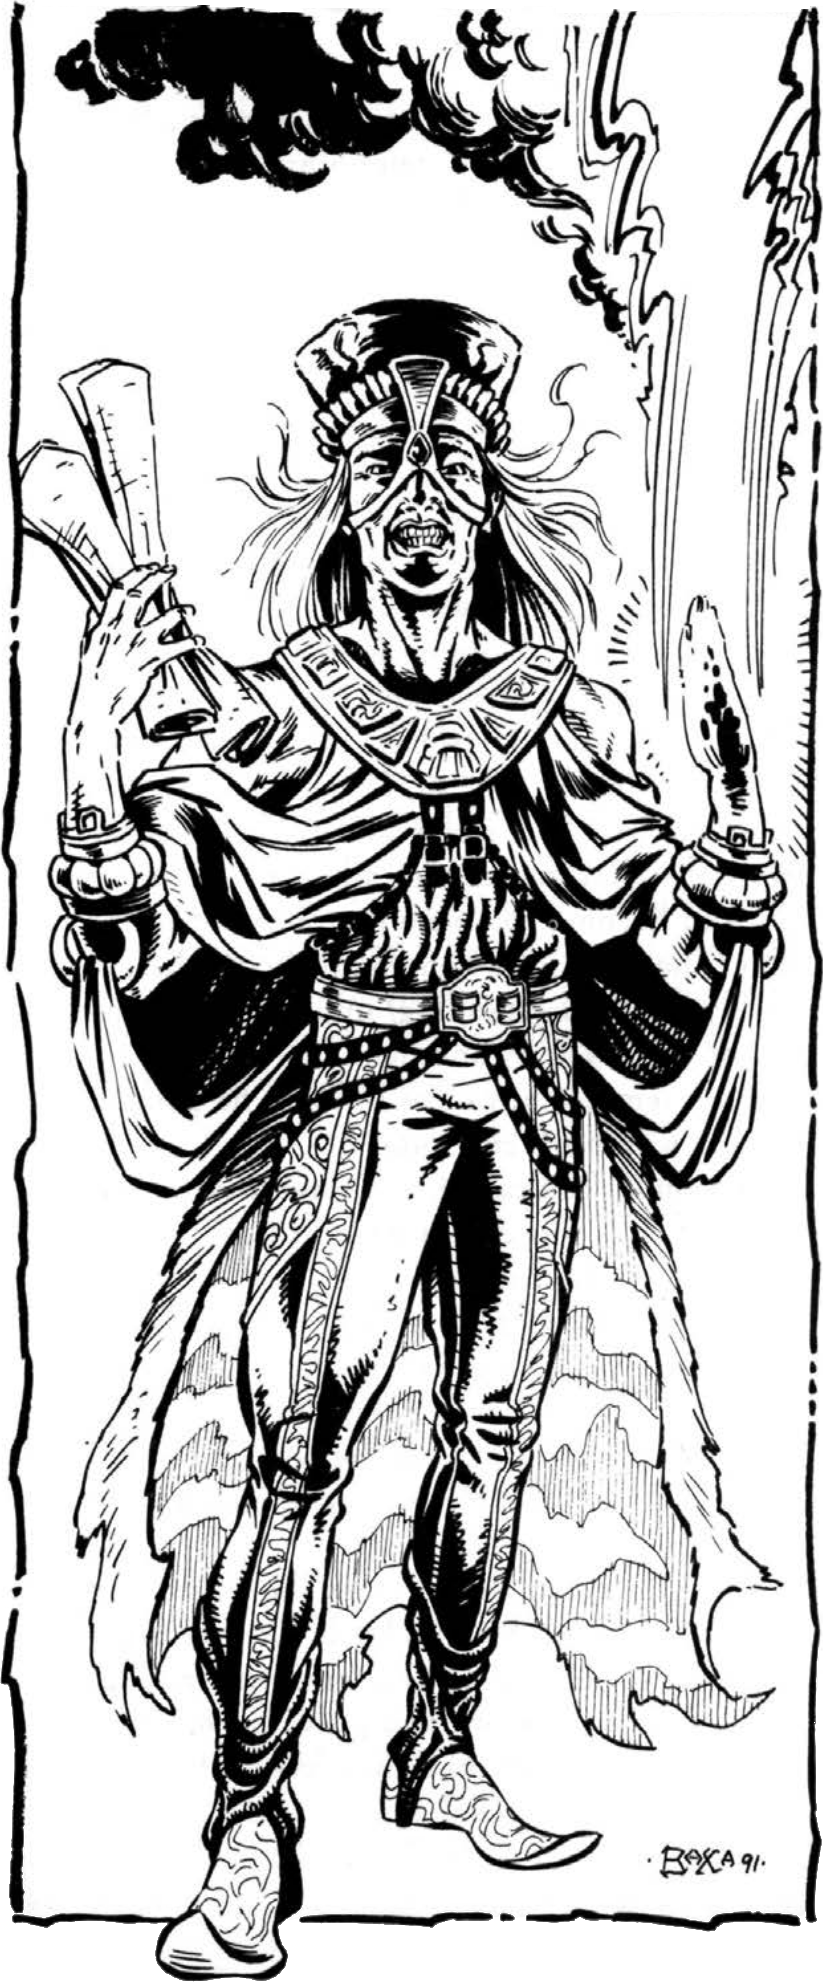
\includegraphics[width=\columnwidth]{images/templar-1.png}
\WOTC
\end{figure}

\subsection{Making a Templar}
Templars can cast a number of divine spells each day, as granted by their lord. If necessary they can be a destructive fighting force, but they serve much better as officers of slave-soldiers, mercenaries, or undead. Their wide array of available skills reflects the equally wide array of roles that Templars fill as servants of the sorcerer-kings and queens.

\textbf{Abilities:} If you want to make good use of your templar spells and you secular aptitude, you'll need a high Charisma. As with any melee-oriented class, Strength is a key ability for templars and Constitution provides you with increased ht points as usual.

\textbf{Races:} While the need for religion and divine magic is nearly universal on Athas, the need for specialized militant priest--bureaucrats is peculiar to large city-states dominated by sorcerer-kings. While in theory, no sentient race is precluded from the templar class, in practice, a sorcerer-king grant spells only to those who he wants to represent him. Humans dominate the templar priesthoods of all city-states except for New Giustenal. Dwarves, muls, and half-elves commonly become templars in many cities, while elves are less commonly accepted. Templars of other races are rare or unheard--of in most cities.

\textbf{Alignment:} A templar's alignment must be within one step of his sorcerer-king's (that is, it may be one step away on either the lawful--chaotic axis or the good--evil axis, but not both). Because of that, templars are almost never good. The laws they uphold are corrupt; the monarchs they serve are arguably the vilest creatures on the face of Athas, and often the templars are cruel and unjust themselves. However, many templars take considerable pride in the prosperity and magnificence of their city-state, and in the well--oiled machine of their order. Templars are most commonly lawful neutral or lawful evil.

\subsection{Game Rule Information}

\textbf{Alignment:} A templar's alignment must be within one step of his sorcerer-monarch's in each axis (that is, it may be one step away on the lawful-chaotic axis or the good-evil axis, but not two steps in either of them). A cleric may not be neutral unless his sorcerer-monarch's alignment is also neutral.

\textbf{Hit Die:} d8.

\subsubsection{Class Skills}
\skill{Appraise} (Int), \skill{Bluff} (Cha), \skill{Concentration} (Con), \skill{Craft} (Int), \skill{Diplomacy} (Cha), \skill{Forgery} (Int), \skill{Gather Information} (Cha), \skill{Heal} (Wis), \skill{Intimidate} (Cha), \skill{Knowledge} (all skills individually) (Int), \skill{Literacy} (N/A), \skill{Profession} (Wis), \skill{Sense Motive} (Wis), \skill{Spellcraft} (Int), and \skill{Spot} (Wis).

\textbf{Skill Points per Level:} 4 + Int modifier ($\times 4$ at 1st level).

\subsubsection{Class Features}

\textbf{Weapon and Armor Proficiency:} Templars are proficient in all simple weapons. Since templar training involves some education in warfare, templars receive two martial weapons proficiencies. Templars are proficient in light and medium armor and shields (except tower shields).

\textbf{Spellcasting:} A templar casts divine spells, which are drawn from the templar spell list. When she gain access to a new level of spells, she automatically knows all the spells for that level on the templar's spell list. She can cast any spell she know without preparing it ahead of time. Essentially, her spell list is the same as her spells known list.

To cast a spell, a templar must have a Charisma score of 10 + the spell's level. The Difficulty Class for a saving throw against a templar's spell is 10 + the spell's level + the templar's Cha modifier. Like other spellcasters, a templar can cast only a certain number of spells of each level per day. The base daily allotment is given on \tabref{The Templar}. In addition, she receives bonus spells if she has a high Charisma score.

She can also cast one domain spell of each spell level per day, as a cleric does. The domain spell is chosen at the time of casting from the spells associated with your assumed domains (see below), as she casts spells spontaneously and need not prepare spells ahead of time.

A templar need not prepare spells in advance. She can cast any spell she knows at any time, assuming she has not yet used up your spells per day for that spell level.

Templars use their sorcerer-king's sigil as divine focus.

\textbf{Assume Domain:} A templar is assigned two domains based on her sorcerer-monarch. Each domain gives her access to a domain spell at each spell level she can cast, from 1st on up, as well as a granted power. She gets the granted powers of both the assumed domains. With access to two domain spells at a given spell level, she adds only one of those spells to your spells known list.

\Table{Sorcerer-Kings' Domains and Alignment}{l X l}{
\tableheader Sorcerer-Monarch & \tableheader Domains & \tableheader Alignment\\
Abalach-Re & Chaos, Charm & Chaotic Evil \\
Andropinis & Law, Nobility & Neutral Evil \\
Borys & Destruction, Protection & Lawful Evil \\
Daskinor & Chaos, Madness & Lawful Evil \\
Dregoth & Death, Destruction & Chaotic Evil \\
Hamanu & Strength, War$\dagger$ & Neutral Evil \\
Kalak & Magic, Trickery & Neutral Evil \\
Lalali-Puy & Animal, Plant & Neutral Evil \\
Nibenay & Magic, Mind & Neutral Evil \\
Oronis & Knowledge, Protection & Neutral Good \\
Tectuktitlay & Glory, Strength & Neutral Evil \\
\rowcolor{white}
\multicolumn{3}{l}{$\dagger$ Hamanu's favored weapon is the longsword.}
}

\textbf{Secular Aptitude (Ex):} A templar gains \feat{Secular Authority} as a bonus feat. In addition, she receives a competence bonus to Secular Authority checks equal to half her class level.

\textit{Sigil} \textbf{(Sp):} Every templar receives a sigil that is the sign of their rank and station as a templar within their city's templarate. The form of the sigil is unique to each city-state, but is always unmistakable for what it is. The sigil serves as your divine focus, and also allows you to use the spell-like powers \spell{arcane mark}, \spell{purify food and drink}, and \spell{slave scent} a combined total of times equal to 3 + your Cha modifier. These spell-like powers do not count against your total of spells per day.

\textbf{Turn or Rebuke Undead (Su):} Any templar, regardless of alignment, has the power to affect undead creatures by channeling the power of his sorcerer-king through his sigil.

A good templar (or a neutral templar who worships a good sorcerer-king) can turn or destroy undead creatures. An evil templar (or a neutral templar who worships an evil sorcerer-king) instead rebukes or commands such creatures. A neutral templar of a neutral sorcerer-king must choose whether his turning ability functions as that of a good templar or an evil templar. Once this choice is made, it cannot be reversed.

A templar may attempt to turn undead a number of times per day equal to 3 + your Charisma modifier. A templar with 5 or more ranks in \skill{Knowledge} (religion) gets a +2 bonus on turning checks against undead. A templar turns undead as a cleric of three levels lower would.

\textbf{Scribe Scroll:} At 6th level, a templar gains \feat{Scribe Scroll} as a bonus feat.

\textbf{Brew Potion:} At 8th level, a templar gains \feat{Brew Potion} as a bonus feat.

\subsubsection{Ex-Templars}
A templar who displeases or abandons his sorcerer-monarch, or one whose sorcerer-monarch dies, loses all templar spellcasting abilities. An ex-templar is treated as a member of an NPC class (commoner, expert, etc) for purposes of determining CR. If the templar later becomes the templar of another sorcerer-monarch, he immediately regains his full templar spellcasting abilities.

\subsection{Playing a Templar}

A templar can take the fighter's place in the front ranks of a party or ensorcel his foes from a distance like a cleric. While you aren't quite as good as either a dedicated fighter or a dedicated cleric or psion in those roles, you're reasonably effective in either, and you can change roles on a round-by-round basis as needed.

As a templar, you believe the acquisition of power and influence is a worthy end in itself. By having power, you can effect your will in the world, be it good or bad. Those who have or seek power deserve your respect, while those who have power but fail to use it deserve your derision.

You adventure out of a desire to gain more power and influence in every quest. Drawn by your power, others follow your lead, and you are happy to command them.

\subsubsection{Religion}
The reverence of templars and their respective sorcerer-monarch varies greatly with the city-state. Some rulers, like Hamanu or Lalali-Puy, claim they are gods and demand their citizen and templars to worship them as such. Other, like Nibenay and Andropinis, only require service, not worship, from their templars.

\subsubsection{Other Classes}
Templars sometimes clash with druids and elemental clerics, who represent an older, more primal relationship between mortal, nature, and the elements. Templars tend to tolerate these ``primitive priests,'' as long as the druids and clerics do not share their opinions that sorcerer-kings are usurpers of profane divine elemental power. Templars get along with most other classes very well, provided of course that a templar is in charge.

\subsubsection{Combat}
Most of a templar's spells target a single target or have a range of touch, so you are most effective when you single out and focus upon defeating a single opponent. Your spells that affect areas are limited mostly to cones,
which means you need to be on or near the front lines to get the greatest effect from them. Even if you come close to being effective as a fighter or cleric in his chosen field, you're certainly not as effective as a fighter and a cleric.

Outside combat, use your secular authority to its greatest advantage, securing troops and resources for when it happens. If you have a cleric or other healer in the group, save your cures for emergency healing, since a cleric can spontaneously convert their spells into healing ones. If no other healer is present, save it to heal yourself and your allies after combat.

\subsubsection{Advancement}
You don't necessarily profit most from remaining a templar throughout your advancement, since you will lose all your spellcasting abilities in case you displease your sorcerer-king, or in the remote possibility your sorcerer-king dies. If you do multiclass, picking an arcane or psionic class is an excellent choice, especially one that has Charisma as a key ability. Alternatively, you might consider beginning your career as either a wizard or as a wilder, then multiclassing into a templar.

Assign as many skill points as possible to \skill{Bluff}, \skill{Diplomacy}, and \skill{Sense Motive}, since these will be helpful in politics even if you are stripped out of your spells. For feats, take the \feat{Negotiator} feat and also consider metamagic feats, such as \feat{Silent Spell} and \feat{Empower Spell}.

\subsection{Starting Packages}
\subsubsection{The Blaster}
Human Templar

\textbf{Ability Scores:} Str 8, Dex 14, Con 13, Int 10, Wis 12, Cha 15.

\textbf{Skills:} \skill{Bluff}, \skill{Concentration}, \skill{Diplomacy}, \skill{Knowledge} (local), \skill{Sense Motive}, \skill{Spellcraft}.

\textbf{Languages:} Common.

\textbf{Feat:} \feat{Combat Casting}, \feat{Weapon Focus} (ranged spell).

\textbf{Weapons:} Macahuitl (1d8/19--20)

Light crossbow with 20 bolts (1d8/19--20, 24 m).

\textbf{Armor:} Leather (+2 AC).

\textbf{Other Gear:} Sigil, standard adventurer's kit, 43 cp.

\subsubsection{The Controller}
Dwarf Templar

\textbf{Ability Scores:} Str 10, Dex 8, Con 14, Int 14, Wis 13, Cha 13.

\textbf{Skills:} \skill{Bluff}, \skill{Diplomacy}, \skill{Intimidate}, \skill{Knowledge} (local), \skill{Sense Motive}.

\textbf{Languages:} Common, Dwarven, Elven, Saurian.

\textbf{Feat:} \skill{Spell Focus} (enchantment).

\textbf{Weapons:} Puchik (1d4/$\times$3)

Light crossbow with 20 bolts (1d8/19--20, 24 m).

\textbf{Armor:} Scale mail (+4 AC).

\textbf{Other Gear:} Sigil, standard adventurer's kit, 34 cp.

\subsubsection{The Politician}
Elf Templar

\textbf{Ability Scores:} Str 8, Dex 14, Con 8, Int 13, Wis 14, Cha 15.

\textbf{Skills:} \skill{Bluff}, \skill{Diplomacy}, \skill{Knowledge} (nobility and royalty), \skill{Literacy}, \skill{Sense Motive}.

\textbf{Languages:} Common, city language, Elven.

\textbf{Feat:} \feat{Negotiator}.

\textbf{Weapons:} Dagger (1d4/19--20, 3 m).

\textbf{Armor:} Leather (+2 AC).

\textbf{Other Gear:} Sigil, standard adventurer's kit, 113 cp.

\subsection{Templars on Athas}
\Quote{Power does not corrupt men. Fools, however, if they get into a position of power, corrupt power.}{Gorg the mad}

Templar duties typically prevent them from adventuring in the standard sense. They often serve missions for their superiors, typically to recover an important item, assassinate a troublemaker, force the hand of a merchant house or barter with an elf tribe. But that is not to say that templars cannot pursue their own interests.

While all templars are technically bound to their civil service positions on a daily basis, a sufficient bribe can buy them a few days of freedom and adventure, as long as they do not get caught going against the interests of their temple or sorcerer-king. Most templars who do adventure, do so for personal power, seeking to acquire items of great power, or for money or fame to impress their lord or superiors.

\subsubsection{Daily Life}
A templar remains ever ready to face the challenges of the Athasian life. Without the need to rest, study or pray for their powers, templars can leap up in pursuit of whatever their templarate requires them to do.

Templars often possess the charisma and take-charge attitude required of great leaders, but many suffer from an inability to empathize with those they lead. Templars respect the pursuit of might and its use, and they often minimize the value of those who adhere to other philosophies. Even among themselves, templars tend to be contentious, battling for power over the cost of another one.

\subsubsection{Notables}
Living in the shadow of their sorcerer-king, templars who develop too much power and influence are usually executed without a second thought. Nonetheless, there are a few who manage to hide their powers and postpone this unavoidable fate. The most famous templar of the Tyr Region managed to do what was thought to be impossible: succeed the throne of a sorcerer-king. Tithian of Mericles helped in the assassination plot to kill King Kalak of Tyr and in return was put into the throne by Agis of Asticles and his allies.

\subsubsection{Organizations}
While not all templars are members of the same bureau or even the same city-state, they all have the same basic organization. These organizations vary dramatically from one place to the other, however. The city-state of Kurn, for instance, only employs those who genuinely wish to protect and serve the people, whereas the members from Eldaarich are chosen only from the most brutal, cruel, and vicious members from the templar's families.

Regardless, a templar's daily life allows little free time. Waking hours not spent in direct service to the templarate, on patrol, or on the field of battle are filled with martial training, divine study, and bureaucratic
activities.

\subsubsection{NPC Reactions}
Templars who do not show affiliation with their city-state's templarate rarely elicit an unusual reaction from others. To most they might seem as a fighter or perhaps a cleric. Those who know or their connection or see evidence of it, such as their sigil or typical clothing react depending on their attitude toward the templar's sorcerer-king (or bureau). This reaction is one step closer to hostile if the sorcerer-monarch is feared or hated by that individual (which is the most likely scenario). The reaction is one step closer to friendly if that individual is directly associated with that sorcerer-monarch. Clerics, druids, and others who are deeply entrenched with a moral outlook view the templar's choice with great suspicion, and their reaction is one step closer to hostile regardless of the templar's sorcerer-monarch.

\subsubsection{Templar Lore}
Characters with ranks in \skill{Knowledge} (local) can research templars to learn more about them. When a character makes a skill check, read or paraphrase the following, including the information from lower DCs.

\textbf{DC 10:} Templars are the minions of the sorcerer-kings and can draw mystical energies from them.

\textbf{DC 15:} A templar dedicates himself to a particular sorcerer-monarch and gains powers based on the sorcerer-monarch chosen. They can control undead, cast divine spells and have control over the city's resources.

\textbf{DC 20:} In addition to the details above, the result allows the PC to know that a templar has a similar connection to their sorcerer-monarch like a cleric and his element, and if that particular sorcerer-monarch dies, the connection is lost and the templar loses all his powers.
% \Class{Wilder}
{Power flows through my veins, beckoning to be released. But if I do, it burns!}{Garath, gith wilder}

For most wilders, psionic power is not a choice, but a discovery. Some wilders discovered their mental powers in childhood or puberty. While psions train in the academies to harness their abilities, wilders tend to discover their powers accidentally and without training. Most wilders never work to harness their powers, lacking the time, inclination or will to further their training. Low-level wilders often think of their power as a handy ``gift'' or ``knack'', rather than a trait that defines them. Generally, only the more focused and powerful will actually identify themselves as ``wilders''.

Wilders often first release their abilities while under great stress. Even as they progress, stress or excitement can flood through a wilder, allowing a display of power beyond his normal range of ability.

\PsychicTable{The Wilder}{
1 & +0 & +0 & +0 & +2 & Wild surge +1, psychic enervation & 2 & 1 & 1st \\
2 & +1 & +0 & +0 & +3 & Elude touch & 6 & 2 & 1st \\
3 & +2 & +1 & +1 & +3 & Wild surge +2 & 11 & 2 & 1st \\
4 & +3 & +1 & +1 & +4 & Surging euphoria +1 & 17 & 3 & 2nd \\
5 & +3 & +1 & +1 & +4 & Volatile mind (1 power point) & 25 & 3 & 2nd \\
6 & +4 & +2 & +2 & +5 && 35 & 4 & 3rd \\
7 & +5 & +2 & +2 & +5 & Wild surge +3 & 46 & 4 & 3rd \\
8 & +6/+1 & +2 & +2 & +6 && 58 & 5 & 4th \\
9 & +6/+1 & +3 & +3 & +6 & Volatile mind (2 power points) & 72 & 5 & 4th \\
10 & +7/+2 & +3 & +3 & +7 && 88 & 6 & 5th \\
11 & +8/+3 & +3 & +3 & +7 & Wild surge +4 & 106 & 6 & 5th \\
12 & +9/+4 & +4 & +4 & +8 & Surging euphoria +2 & 126 & 7 & 6th \\
13 & +9/+4 & +4 & +4 & +8 & Volatile mind (3 power points) & 147 & 7 & 6th \\
14 & +10/+5 & +4 & +4 & +9 && 170 & 8 & 7th \\
15 & +11/+6/+1 & +5 & +5 & +9 & Wild surge +5 & 195 & 8 & 7th \\
16 & +12/+7/+2 & +5 & +5 & +10 && 221 & 9 & 8th \\
17 & +12/+7/+2 & +5 & +5 & +10 & Volatile mind (4 power points) & 250 & 9 & 8th \\
18 & +13/+8/+3 & +6 & +6 & +11 && 280 & 10 & 9th \\
19 & +14/+9/+4 & +6 & +6 & +11 & Wild surge +6 & 311 & 10 & 9th \\
20 & +15/+10/+5 & +6 & +6 & +12 & Surging euphoria +3 & 343 & 11 & 9th
}

\begin{figure}[t!]
\centering
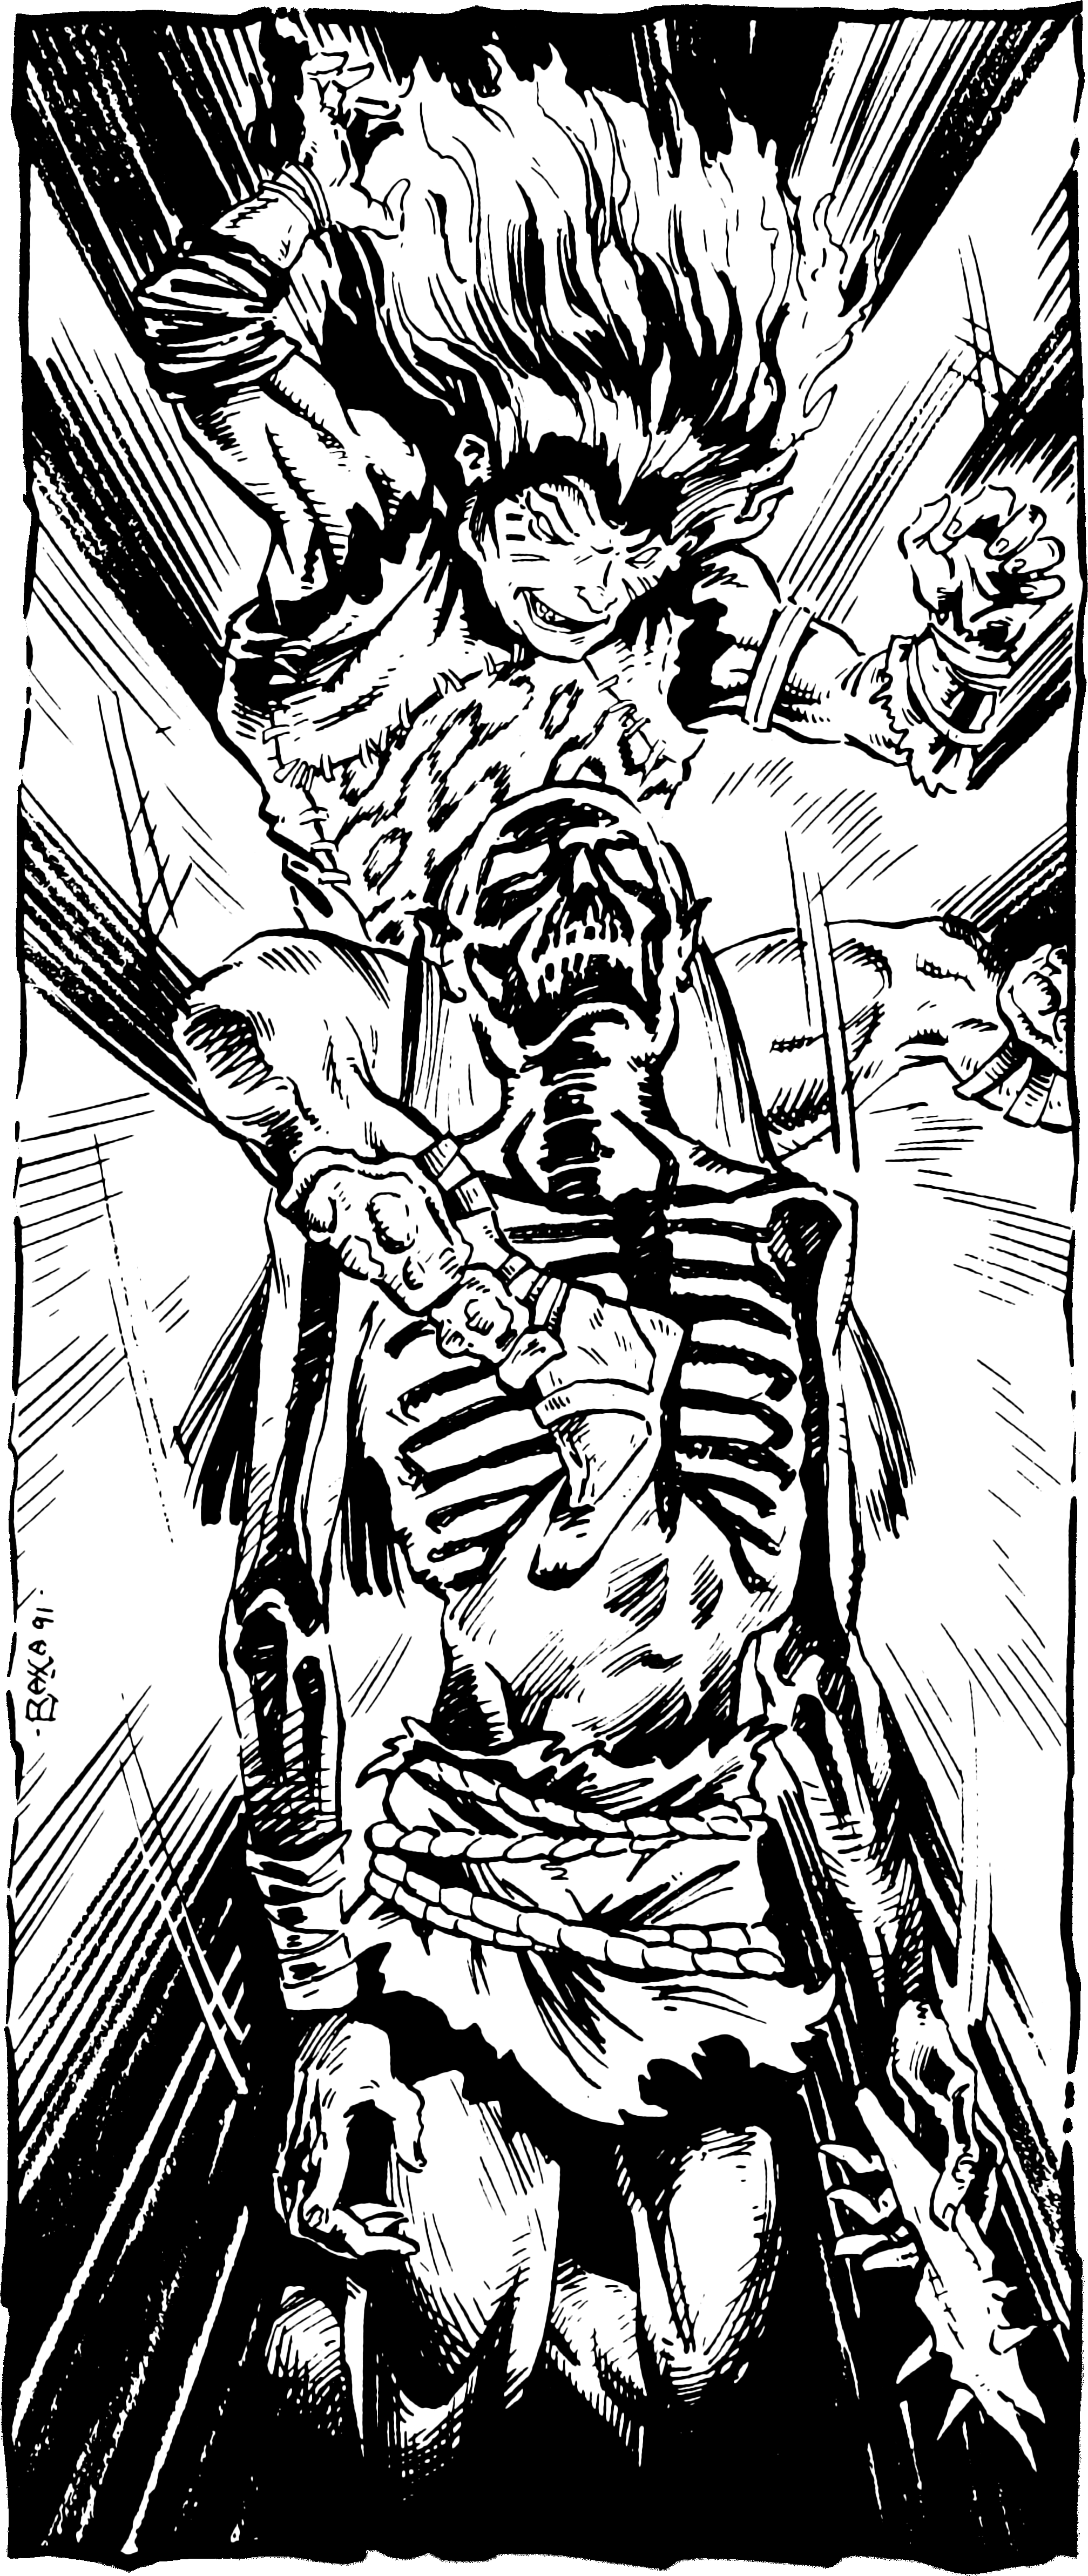
\includegraphics[width=\columnwidth]{images/psionic-1.png}
\par\textit{\small\textcopyright Wizards of the Coast, 2020.}
\end{figure}

\subsection{Making a Wilder}

Through experience, the wilder discovers supernatural powers that are an extension of his personality. Wilders know fewer powers than other manifesting classes, but their wild surge ability gives their powers greater flexibility. These surges are not without cost, however, and can have a great toll on the careless wilder.

\textbf{Races:} Psionic talent is common in the tablelands. Because of the limited access to psionic instruction, humans elves, halflings, and to a lesser extent, muls, are much more likely to be wilders than psions. Races that are less charismatic, less individualistic, and less prone to emotion, such as thri-kreen and dwarves rarely become wilders; more of them become psions or psychic warriors. The pterran culture glorifies the path of the psion, so wilders are rare. Half-giants tend to become wilders rather than psions, because even with psionic training, many half-giants lack the wit, Will, or focus to excel as psions.

\textbf{Alignment:} Though wilders have no inclinations towards good or evil, as a whole they tend to be chaotic.

\subsection{Game Rule Information}

\textbf{Hit Die:} d6.

\subsubsection{Class Skills}
\skill{Autohypnosis} (Wis), \skill{Balance} (Dex), \skill{Bluff} (Cha), \skill{Climb} (Str), \skill{Concentration} (Con), \skill{Craft} (Int), \skill{Escape Artist} (Dex), \skill{Intimidate} (Cha), \skill{Jump} (Str), \skill{Knowledge} (psionics) (Int), \skill{Listen} (Wis), \skill{Profession} (Wis), \skill{Psicraft} (Int), \skill{Sense Motive} (Wis), \skill{Spot} (Wis), \skill{Survival} (Wis), and \skill{Tumble} (Dex).

\textbf{Skill Points per Level:} 4 + Int modifier ($\times 4$ at 1st level).

\subsubsection{Class Features}

\textbf{Weapon and Armor Proficiency:} Wilders are proficient with all simple weapons, with light armor, and with shields (except tower shields).

\textbf{Power Points/Day:} A wilder's ability to manifest powers is limited by the power points she has available. Her base daily allotment of power points is given on \tabref{The Wilder}. In addition, she receives bonus power points per day if she has a high Charisma score (see \tabref{Ability Scores and Bonus Power Points}). Her race may also provide bonus power points per day, as may certain feats and items.

\textbf{Powers Known:} A wilder begins play knowing one wilder power of your choice. At every even-numbered class level after 1st, she unlocks the knowledge of new powers.

Choose the powers known from the wilder power list. (Exception: The feat \feat{Expanded Knowledge} do allow a wilder to learn powers from the lists of other classes.) A wilder can manifest any power that has a power point cost equal to or lower than her manifester level.

The total number of powers a wilder can manifest in a day is limited only by her daily power points.

A wilder simply knows her powers; they are ingrained in her mind. She does not need to prepare them (in the way that some spellcasters prepare their spells), though she must get a good night's sleep each day to regain all her spent power points.

The Difficulty Class for saving throws against wilder powers is 10 + the power's level + the wilder's Charisma modifier.

\textbf{Maximum Power Level Known:} A wilder begins play with the ability to learn 1st-level powers. As she attains higher levels, she may gain the ability to master more complex powers.

To learn or manifest a power, a wilder must have a Charisma score of at least 10 + the power's level.

\textbf{Wild Surge (Su):} A wilder can let her passion and emotion rise to the surface in a wild surge when she manifests a power. During a wild surge, a wilder gains phenomenal psionic strength, but may harm herself by the reckless use of her power (see Psychic Enervation, below).

A wilder can choose to invoke a wild surge whenever she manifests a power. When she does so, she gains +1 to her manifester level with that manifestation of the power. The manifester level boost gives her the ability to augment her powers to a higher degree than she otherwise could; however, she pays no extra power point for this wild surge. Instead, the additional 1 power point that would normally be required to augment the power is effectively supplied by the wild surge.

Level-dependent power effects are also improved, depending on the power a wilder manifests with her wild surge.

This improvement in manifester level does not grant her any other benefits (psicrystal abilities do not advance, she does not gain higher-level class abilities, and so on).

She cannot use the \feat{Overchannel} psionic feat and invoke her wild surge at the same time.

At 3rd level, a wilder can choose to boost her manifester level by two instead of one. At 7th level, she can boost her manifester level by up to three; at 11th level, by up to four; at 15th level, by up to five; and at 19th level, by up to six.

In all cases, the wild surge effectively pays the extra power point cost that is normally required to augment the power; only the unaugmented power point cost is subtracted from the wilder's power point reserve.

\textbf{Psychic Enervation (Ex):} Pushing oneself by invoking a wild surge is dangerous. Immediately following each wild surge, a wilder may be overcome by the strain of her effort. The chance of suffering psychic enervation is equal to 5\% per manifester level added with the wild surge.

A wilder who is overcome by psychic enervation is dazed until the end of her next turn and loses a number of power points equal to her wilder level.

\textbf{Elude Touch (Ex):} Starting at 2nd level, a wilder's intuition supersedes her intellect, alerting her to danger from touch attacks (including rays). She gains a bonus to Armor Class against all touch attacks equal to her Charisma bonus; however, her touch AC can never exceed her Armor Class against normal attacks.

\textbf{Surging Euphoria (Ex):} Starting at 4th level, when a wilder uses her wild surge ability, she gains a +1 morale bonus on attack rolls, damage rolls, and saving throws for a number of rounds equal to the intensity of her wild surge.

If a wilder is overcome by psychic enervation following her wild surge, she does not gain the morale bonus for this use of her wild surge ability.

At 12th level, the morale bonus on a wilder's attack rolls, damage rolls, and saving throws increases to +2. At 20th level, the bonus increases to +3.

\textbf{Volatile Mind (Ex):} A wilder's temperamental mind is hard to encompass with the discipline of telepathy. When any telepathy power is manifested on a wilder of 5th level or higher, the manifester of the power must pay 1 power point more than he otherwise would have spent.

The extra cost is not a natural part of that power's cost. It does not augment the power; it is simply a wasted power point. The wilder's volatile mind can force the manifester of the telepathy power to exceed the normal power point limit of 1 point per manifester level. If the extra cost raises the telepathy power's cost to more points than the manifester has remaining in his reserve, the power simply fails, and the manifester exhausts the rest of his power points.

At 9th level, the penalty assessed against telepathy powers manifested on a wilder is increased to 2 power points. At 13th level, the penalty increases to 3 power points, and at 17th level it increases to 4 power points.

As a standard action, a wilder can choose to lower this effect for 1 round.

\subsection{Playing a Wilder}
As a wilder, you adventure to practice your abilities and gain further understanding and mastery about the Will. You are very passionate about your powers, and you often push yourself to your limits with your wild surges, but you are not blind to its dangers.

\subsubsection{Religion}
Although wilders, like psions, draw their energies from within, wilder powers require less focus and discipline, so wilders are as likely as any other Athasian to be religious. A wilders religion can have a great impact on his power selection. A wilder who worships fire, for example, often discovers powers that involve light, heat or flame.

\subsubsection{Other Classes}
Wilder's opinions vary wildly. Some wilders view psions with awe, respecting the psion's greater knowledge and control; others chafe under the psion's perceived superiority complex.

\subsubsection{Combat}
In combat, you use your impressive array of psionic powers for both attack and defense against your enemies and opponents, just as any other psionicist would. Of course, as a wilder, you can call upon swells of psionic potential that other psionicists cannot access in the form of wild surges.

\subsubsection{Advancement}
Your interest on psionics is more than academic---it has been your motivating force for years. Perhaps you became a wilder after witnessing one destroying an entire village during one of his surges, or you vowed to gain control of the power you first displayed in your puberty every time you got were angered. Whatever the case, since the day you first became a wilder, you've worked to master a power more primal than spells and stronger than steel.

The powers you choose strongly shape your abilities. You are heavily invested in combat prowess as a result of the erratic and emotional nature of your power, but you have some flexibility in how you learn your powers. If you choose only offensive powers, you will have few defenses and limited versatility beyond combat, but you'll be devastating even in dire situations. If you focus on other powers, you will have more options outside a fight, but you might have only area attacks that could accidentally hurt a friend.

\vskip5cm
\subsection{Starting Packages}
\subsubsection{The Battle Wilder}
Mul Wilder

\textbf{Ability Scores:} Str 17, Dex 8, Con 16, Int 10, Wis 12, Cha 13.

\textbf{Skills:} \skill{Concentration}, \skill{Intimidate}, \skill{Psicraft}.

\textbf{Languages:} Common.

\textbf{Feat:} \feat{Combat Manifestation}.

\textbf{Weapons:} Longspear (1d8/$\times$3).

\textbf{Armor:} Scale mail (+4 AC).

\textbf{Other Gear:} Standard adventurer's kit, 20 cp.

\subsubsection{The Blaster}
Human Wilder

\textbf{Ability Scores:} Str 8, Dex 14, Con 13, Int 12, Wis 10, Cha 15.

\textbf{Skills:} \skill{Concentration}, \skill{Intimidate}, \skill{Knowledge} (psionics), \skill{Psicraft}.

\textbf{Languages:} Common.

\textbf{Feat:} \feat{Lightning Reflexes}, \feat{Psionic Endowment}.

\textbf{Weapons:} Spear (1d8/$\times$3, 6 m)

Light crossbow with 20 bolts (1d8/19--20, 24 m).

\textbf{Armor:} Leather (+2 AC).

\textbf{Other Gear:} Standard adventurer's kit, 26 cp.

\subsubsection{The Sharpshooter}
Halfling Wilder

\textbf{Ability Scores:} Str 6, Dex 16, Con 13, Int 12, Wis 10, Cha 15.

\textbf{Skills:} \skill{Concentration}, \skill{Intimidate}, \skill{Spot} (cc).

\textbf{Languages:} Halfling.

\textbf{Feat:} \feat{Point Blank Shot}.

\textbf{Weapons:} Spear (1d8/$\times$3, 6 m)

Light crossbow with 20 bolts (1d8/19--20, 24 m).

\textbf{Armor:} Leather (+2 AC).

\textbf{Other Gear:} Standard adventurer's kit, 26 cp.

\subsection{Wilders on Athas}
\Quote{Something seemed strange the second I saw Nakua's face. It's odd. He acted like a different person. My friend Kuko asked him if he was really Nakua or if he was someone else. And those were his last words}{Ekee, elven dancer}

Psionic is very common on Athas, and wilders can be widely found in the Tablelands, representing psionic energy in its most raw state, and change for change's sake. Neutral wilders are rare, but such characters become famous within the ranks of their comrades, since their vision is unclouded by moral concerns.

Wilders know that using psionic powers can be strenuous, and the limit of a character's endurance is his Will. Eventually, even the most powerful of masters becomes exhausted and must rest to replenish his strength. When wounds and exhaustion cloud the vision and the mind swims in delirium, only the greatest wilders possess the Will to continue using their powers.

\subsubsection{Daily Life}

Wilders spend their days in travel and contemplation, with an occasional rant and wild outburst (usually against the foes an adventurer comes across). They enjoy talking about their psionic abilities and about their life philosophies.

\subsubsection{Notables}

The xenophobic Kenkus (FFN 126) are the race to most commonly sport wilders, although no one knows for sure why. Elves, due to their chaotic nature, also seem to have a higher rate of wilders in their milieu.

\subsubsection{Organizations}

A wilder's path is his own to thread, since no overarching organization exists to recruit you into its ranks. Most wilders are just too erratic and freedom-loving to join one, anyway.

\subsubsection{NPC Reactions}

Most people do not understand the difference between a psion and a wilder, so their attitudes span the spectrum. Psions NPC attitudes range from indifferent to unfriendly, although most psiologists (page 104) tend to have their attitude bent towards hostile.

\subsubsection{Wilder Lore}

Characters with ranks in \skill{Knowledge} (psionics) can research wilders to learn more about them. When a character makes a skill check, read or paraphrase the following, including the information from lower DCs.

\textbf{DC 10:} A wilder is a kind of psionicist that can trigger a surge of psionic power beyond control.

\textbf{DC 15:} Wilders usually become very weak, both physically and mentally, after unleashing their psionic surges.

\textbf{DC 20:} Experienced wilders learn how to further tap into their Will and manage to also strengthen their bodies while surging.
\Class{Wizard}
{So what if the land becomes barren? It's not like we're going to stick around.}{Datuu Dawnchaser, elf defiler}

Athasian wizards drain energy from the surrounding soil. The method used labels the wizard as a defiler or a preserver. Preservers have the self-control to gather energy without destroying plants. Those who do not, or who feel no remorse about the damage caused, become Defilers. Defilers leave behind sterile soil and infertile ash when they cast spells. Because of this, most wastelanders blame wizards for the desert landscape that dominates the Tablelands today, and their hatred extends to defilers and preservers alike. In the seven cities, arcane magic is outlawed and feared.

Writing is also illegal in the Tablelands, thus wizards have to go to great lengths to conceal their spellbooks, and they have refined this art to the point where even fellow wizards can be hard pressed to identify a spell book. When found, they are precious resources, hoarded and studied by wizards thirsty for knowledge or power.

\SpellcasterTable{The Wizard}{.3cm}{
1st & +0 & +0 & +0 & +2 & Path, summon familiar, \feat{Scribe Scroll} & 3 & 1 &&&&&&&&\\
2nd & +1 & +0 & +0 & +3 &  & 4 & 2 &&&&&&&&\\
3rd & +1 & +1 & +1 & +3 &  & 4 & 2 & 1 &&&&&&&\\
4th & +2 & +1 & +1 & +4 &  & 4 & 3 & 2 &&&&&&&\\
5th & +2 & +1 & +1 & +4 & Bonus feat & 4 & 3 & 2 & 1 &&&&&&\\
6th & +3 & +2 & +2 & +5 &  & 4 & 3 & 3 & 2 &&&&&&\\
7th & +3 & +2 & +2 & +5 &  & 4 & 4 & 3 & 2 & 1 &&&&&\\
8th & +4 & +2 & +2 & +6 &  & 4 & 4 & 3 & 3 & 2 &&&&&\\
9th & +4 & +3 & +3 & +6 &  & 4 & 4 & 4 & 3 & 2 & 1 &&&&\\
10th & +5 & +3 & +3 & +7 & Bonus feat & 4 & 4 & 4 & 3 & 3 & 2 &&&&\\
11th & +5 & +3 & +3 & +7 &  & 4 & 4 & 4 & 4 & 3 & 2 & 1 &&&\\
12th & +6/+1 & +4 & +4 & +8 &  & 4 & 4 & 4 & 4 & 3 & 3 & 2 &&&\\
13th & +6/+1 & +4 & +4 & +8 &  & 4 & 4 & 4 & 4 & 4 & 3 & 2 & 1 &&\\
14th & +7/+2 & +4 & +4 & +9 &  & 4 & 4 & 4 & 4 & 4 & 3 & 3 & 2 &&\\
15th & +7/+2 & +5 & +5 & +9 & Bonus feat & 4 & 4 & 4 & 4 & 4 & 4 & 3 & 2 & 1 &\\
16th & +8/+3 & +5 & +5 & +10 &  & 4 & 4 & 4 & 4 & 4 & 4 & 3 & 3 & 2 &\\
17th & +8/+3 & +5 & +5 & +10 &  & 4 & 4 & 4 & 4 & 4 & 4 & 4 & 3 & 2 & 1\\
18th & +9/+4 & +6 & +6 & +11 &  & 4 & 4 & 4 & 4 & 4 & 4 & 4 & 3 & 3 & 2\\
19th & +9/+4 & +6 & +6 & +11 &  & 4 & 4 & 4 & 4 & 4 & 4 & 4 & 4 & 3 & 3\\
20th & +10/+5 & +6 & +6 & +12 & Bonus feat & 4 & 4 & 4 & 4 & 4 & 4 & 4 & 4 & 4 & 4
}

\subsection{Making a Wizard}
The wizard's greatest strength is also his greatest liability. Often wizards will conceal their abilities, learning to mask their spellcasting behind other actions. For all but the most powerful wizards, secrecy is of prime importance, and some will not exercise their power in the presence of those that they do not feel they can trust. Because of this, and because of their generally frail nature, wizards can often be seen as a liability by those not aware of the power they hide.

\textbf{Races:} Elves and humans are the most likely to be wizards. Elves are more tolerant of the faults of magic, even at its worst, due to their nomadic nature. Defiling simply isn't as much of a concern if the ruined land is fifty miles behind you by the end of the next day. The solitary life lead by most half-elves makes it easier for them to conceal their wizardry, should they choose to follow that path. Some rare halflings and pterrans will take up the arts of wizardry, but these races are so closely tuned to flow of life on Athas that they will never willingly defile. Half-giants, trusting and slow-witted, rarely become wizards, and those that do rarely survive for long. Dwarves rarely take to the magic arts, though their focus allows those that do to become exceptionally skilled. Thri-kreen and muls almost never become wizards.

\textbf{Alignment:} Overall, most wizards display a tendency towards lawfulness. The self-control and restraint necessary to keep oneself secret, as well as the disciplined need for long days of studying take their toll on many of the less careful wizards. Most wizards of good alignment have developed the skill and control necessary to master preserving, and only in the direst of situations would a good-aligned wizard defile. Neutral or evil wizards, however, are more likely to become defilers, though evil preservers are not unheard of.

\subsection{Game Rule Information}

\textbf{Alignment:} Preservers can be of any alignment. Defilers must be of any nongood.

\textbf{Hit Die:} d4.

\subsubsection{Class Skills}
\skill{Bluff} (Cha), \skill{Concentration} (Con), \skill{Craft} (Int), \skill{Decipher Script} (Int), \skill{Disguise} (Cha), \skill{Knowledge} (all skills, taken individually) (Int), \skill{Literacy} (N/A), \skill{Profession} (Wis), and \skill{Spellcraft} (Int).

\textbf{Skill Points per Level:} 2 + Int modifier ($\times4$ at 1st level).

\subsubsection{Class Features}
\textbf{Weapon and Armor Proficiency:} Wizards are proficient with the club, dagger, heavy crossbow, light crossbow, and quarterstaff, but not with any type of armor or shield. Armor of any type interferes with a wizard's movements, which can cause her spells with somatic components to fail.

\textbf{Spells:} A wizard casts arcane spells which are drawn from the wizard spell list. A wizard must choose and prepare her spells ahead of time (see below).

To learn, prepare, or cast a spell, the wizard must have an Intelligence score equal to at least 10 + the spell level. The Difficulty Class for a saving throw against a wizard's spell is 10 + the spell level + the wizard's Intelligence modifier.

Like other spellcasters, a wizard can cast only a certain number of spells of each spell level per day. Her base daily spell allotment is given on \tabref{The Wizard}. In addition, she receives bonus spells per day if she has a high Intelligence score.

A wizard may know any number of spells. She must choose and prepare her spells ahead of time by getting a good night's sleep and spending 1 hour studying her spellbook. While studying, the wizard decides which spells to prepare.

\begin{figure*}[b!]
\centering
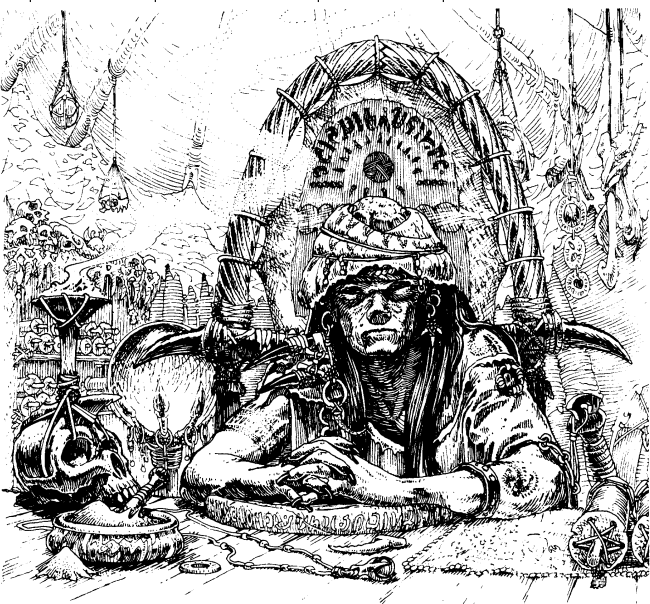
\includegraphics[width=\textwidth-2cm]{images/wizard-5.png}
\WOTC
\end{figure*}

\textbf{Bonus Languages:} A wizard may substitute Draconic for one of the bonus languages available to the character because of her race.

\textbf{Familiar:} A wizard can obtain a familiar. Doing so takes 24 hours and uses up magical materials that cost 100 ceramic pieces. A familiar is a magical beast that resembles a small animal and is unusually tough and intelligent. The creature serves as a companion and servant.

The wizard chooses the kind of familiar he gets. As the wizard advances in level, his familiar also increases in power.

If the familiar dies or is dismissed by the wizard, the wizard must attempt a DC 15 Fortitude saving throw. Failure means he loses 200 experience points per wizard level; success reduces the loss to one-half that amount. However, a wizard's experience point total can never go below 0 as the result of a familiar's demise or dismissal. A slain or dismissed familiar cannot be replaced for a year and day. A slain familiar can be raised from the dead just as a character can be, and it does not lose a level or a Constitution point when this happy event occurs.

A character with more than one class that grants a familiar may have only one familiar at a time.

\textbf{Scribe Scroll:} At 1st level, a wizard gains \feat{Scribe Scroll} as a bonus feat.

\textbf{Path:} At 1st level, a wizard must choose a philosophical path: preservation or defilement. This choice is not final. Preservers can defile and be corrupted, and defilers can get redemption.

\textit{Path Dexter:} Wizards who take this path are preservers. They master the balance of the arcane, casting spells with no collateral environmental damage.

Preservers learn one spell at each wizard level from abjuration or divination schools. They are drawn to protection and information spells.

\textit{Path Sinister:} This path is allowed only for nongood wizards. The wizards who take this path are defilers. With every spell cast, defilers take the life out of the plants and soil around them.

Defilers learn one spell at each wizard level from evocation or necromancy schools. They best utilize those darker and more destructive schools.

\textbf{Bonus Feats:} At 5th, 10th, 15th, and 20th level, a wizard gains a bonus feat. At each such opportunity, she can choose a metamagic feat, a raze feat, an item creation feat, or \feat{Spell Mastery}. The wizard must still meet all prerequisites for a bonus feat, including caster level minimums.

These bonus feats are in addition to the feat that a character of any class gets from advancing levels. The wizard is not limited to the categories of item creation feats, metamagic feats, or Spell Mastery when choosing these feats.

\textbf{Spellbooks:} A wizard must study her spellbook each day to prepare her spells. She cannot prepare any spell not recorded in her spellbook, except for read magic, which all wizards can prepare from memory.

A wizard begins play with a spellbook containing all 0-level wizard spells (except those from her prohibited school or schools, if any; see School Specialization, below) plus three 1st-level spells of your choice. For each point of Intelligence bonus the wizard has, the spellbook holds one additional 1st-level spell of your choice.

At each new wizard level, she gains three new spells of any spell level or levels that she can cast (based on her new wizard level) for her spellbook, one of which must be from her path's schools. At any time, a wizard can also add spells found in other wizards' spellbooks to her own.

\subsubsection{Familiars}
A familiar is a normal animal that gains new powers and becomes a magical beast when summoned to service by a wizard. It retains the appearance, Hit Dice, base attack bonus, base save bonuses, skills, and feats of the normal animal it once was, but it is treated as a magical beast instead of an animal for the purpose of any effect that depends on its type. Only a normal, unmodified animal may become a familiar. An animal companion cannot also function as a familiar.

A familiar also grants special abilities to its master, as given on the table below. These special abilities apply only when the master and familiar are within 1.5 kilometer of each other.

Levels of different classes that are entitled to familiars stack for the purpose of determining any familiar abilities that depend on the master's level.

\Table{Familiars}{l X}{
	\tableheader Familiar & \tableheader Special\\
	Bat & Master gains a +3 bonus on \skill{Listen} checks\\
	Cat & Master gains a +3 bonus on \skill{Move Silently} checks\\
	Dustgull & Master gains a +3 bonus on \skill{Spot} checks\\
	Hawk & Master gains a +3 bonus on \skill{Spot} checks in bright light\\
	Kes'trekel & Master gains a +2 bonus on Reflex saves\\
	Lizard & Master gains a +3 bonus on \skill{Climb} checks\\
	Owl & Master gains a +3 bonus on \skill{Spot} checks in shadows\\
	Rat & Master gains a +2 bonus on Fortitude saves\\
	Raven$\dagger$ & Master gains a +3 bonus on \skill{Appraise} checks\\
	Skyfish & Master gains a +3 bonus on \skill{Swim} checks\\
	Sygra & Master gains a +3 hit points\\
	Tiny viper & Master gains a +3 bonus on \skill{Bluff} checks\\
	% Toad & Master gains +3 hit points\\
	% Weasel & Master gains a +2 bonus on Reflex saves
	\rowcolor{white}
	\multicolumn{2}{p{\columnwidth}}{$\dagger$ A raven familiar can speak one language of its master's choice as a supernatural ability.}
}


\textbf{Familiar Basics:} Use the basic statistics for a creature of the familiar's kind, but make the following changes:

\textit{Hit Dice:} For the purpose of effects related to number of Hit Dice, use the master's character level or the familiar's normal HD total, whichever is higher.

\textit{Hit Points:} The familiar has one-half the master's total hit points (not including temporary hit points), rounded down, regardless of its actual Hit Dice.

\textit{Attacks:} Use the master's base attack bonus, as calculated from all his classes. Use the familiar's Dexterity or Strength modifier, whichever is greater, to get the familiar's melee attack bonus with natural weapons.

Damage equals that of a normal creature of the familiar's kind.

\textit{Saving Throws:} For each saving throw, use either the familiar's base save bonus (Fortitude +2, Reflex +2, Will +0) or the master's (as calculated from all his classes), whichever is better. The familiar uses its own ability modifiers to saves, and it doesn't share any of the other bonuses that the master might have on saves.

\textit{Skills:} For each skill in which either the master or the familiar has ranks, use either the normal skill ranks for an animal of that type or the master's skill ranks, whichever are better. In either case, the familiar uses its own ability modifiers. Regardless of a familiar's total skill modifiers, some skills may remain beyond the familiar's ability to use.

\Table{Familiar Progression}{b{1.4cm} Z{1.2cm} c X}{
	\tableheader Master Class Level & \tableheader Natural Armor Adj. & \tableheader Int & \tableheader Special\\
	1st--2nd & +1 & 6 & Alertness, improved evasion, share spells, empathic link\\
	3rd--4th & +2 & 7 & Deliver touch spells\\
	5th--6th & +3 & 8 & Speak with master\\
	7th--8th & +4 & 9 & Speak with animals of its kind\\
	9th--10th & +5 & 10 & \\
	11th--12th & +6 & 11 & Spell resistance\\
	13th--14th & +7 & 12 & Scry on familiar\\
	15th--16th & +8 & 13 & \\
	17th--18th & +9 & 14 & \\
	19th--20th & +10 & 15 &
}

\textbf{Familiar Ability Descriptions:} All familiars have special abilities (or impart abilities to their masters) depending on the master's combined level in classes that grant familiars, as shown on the table above. The abilities given on the table are cumulative.

\textit{Natural Armor Adj.:} The number noted here is an improvement to the familiar's existing natural armor bonus.

\textit{Int:} The familiar's Intelligence score.

\textit{Alertness (Ex):} While a familiar is within arm's reach, the master gains the Alertness feat.

\textit{Improved Evasion (Ex):} When subjected to an attack that normally allows a Reflex saving throw for half damage, a familiar takes no damage if it makes a successful saving throw and half damage even if the saving throw fails.

\textit{Share Spells:} At the master's option, he may have any spell (but not any spell-like ability) he casts on himself also affect his familiar. The familiar must be within 1.5 meter at the time of casting to receive the benefit.

If the spell or effect has a duration other than instantaneous, it stops affecting the familiar if it moves farther than 1.5 meter away and will not affect the familiar again even if it returns to the master before the duration expires. Additionally, the master may cast a spell with a target of ``You'' on his familiar (as a touch range spell) instead of on himself.

A master and his familiar can share spells even if the spells normally do not affect creatures of the familiar's type (magical beast).

\textit{Empathic Link (Su):} The master has an empathic link with his familiar out to a distance of up to 1.5 kilometer. The master cannot see through the familiar's eyes, but they can communicate empathically. Because of the limited nature of the link, only general emotional content can be communicated.

Because of this empathic link, the master has the same connection to an item or place that his familiar does.

\textit{Deliver Touch Spells (Su):} If the master is 3rd level or higher, a familiar can deliver touch spells for him. If the master and the familiar are in contact at the time the master casts a touch spell, he can designate his familiar as the ``toucher.'' The familiar can then deliver the touch spell just as the master could. As usual, if the master casts another spell before the touch is delivered, the touch spell dissipates.

\textit{Speak with Master (Ex):} If the master is 5th level or higher, a familiar and the master can communicate verbally as if they were using a common language. Other creatures do not understand the communication without magical help.

\textit{Speak with Animals of Its Kind (Ex):} If the master is 7th level or higher, a familiar can communicate with animals of approximately the same kind as itself (including dire varieties): bats with bats, rats with rodents, cats with felines, hawks and owls and ravens with birds, lizards and snakes with reptiles, toads with amphibians, weasels with similar creatures (weasels, minks, polecats, ermines, skunks, wolverines, and badgers). Such communication is limited by the intelligence of the conversing creatures.

\textit{Spell Resistance (Ex):} If the master is 11th level or higher, a familiar gains spell resistance equal to the master's level + 5. To affect the familiar with a spell, another spellcaster must get a result on a caster level check (1d20 + caster level) that equals or exceeds the familiar's spell resistance.

\textit{Scry on Familiar (Sp):} If the master is 13th level or higher, he may scry on his familiar (as if casting the scrying spell) once per day.

\subsubsection{School Specialization}
A school is one of eight groupings of spells, each defined by a common theme. If desired, a wizard may specialize in one school of magic (see below). Specialization allows a wizard to cast extra spells from her chosen school, but she then never learns to cast spells from some other schools.

A specialist wizard can prepare one additional spell of her specialty school per spell level each day. She also gains a +2 bonus on \skill{Spellcraft} checks to learn the spells of her chosen school.

The wizard must choose whether to specialize and, if she does so, choose her specialty at 1st level. At this time, she must also give up two other schools of magic (unless she chooses to specialize in divination; see below), which become her prohibited schools.

A wizard can never give up divination to fulfill this requirement.

Spells of the prohibited school or schools are not available to the wizard, and she can't even cast such spells from scrolls or fire them from wands. She may not change either her specialization or her prohibited schools later.

The eight schools of arcane magic are abjuration, conjuration, divination, enchantment, evocation, illusion, necromancy, and transmutation.

Spells that do not fall into any of these schools are called universal spells.

\begin{figure}[t!]
\centering
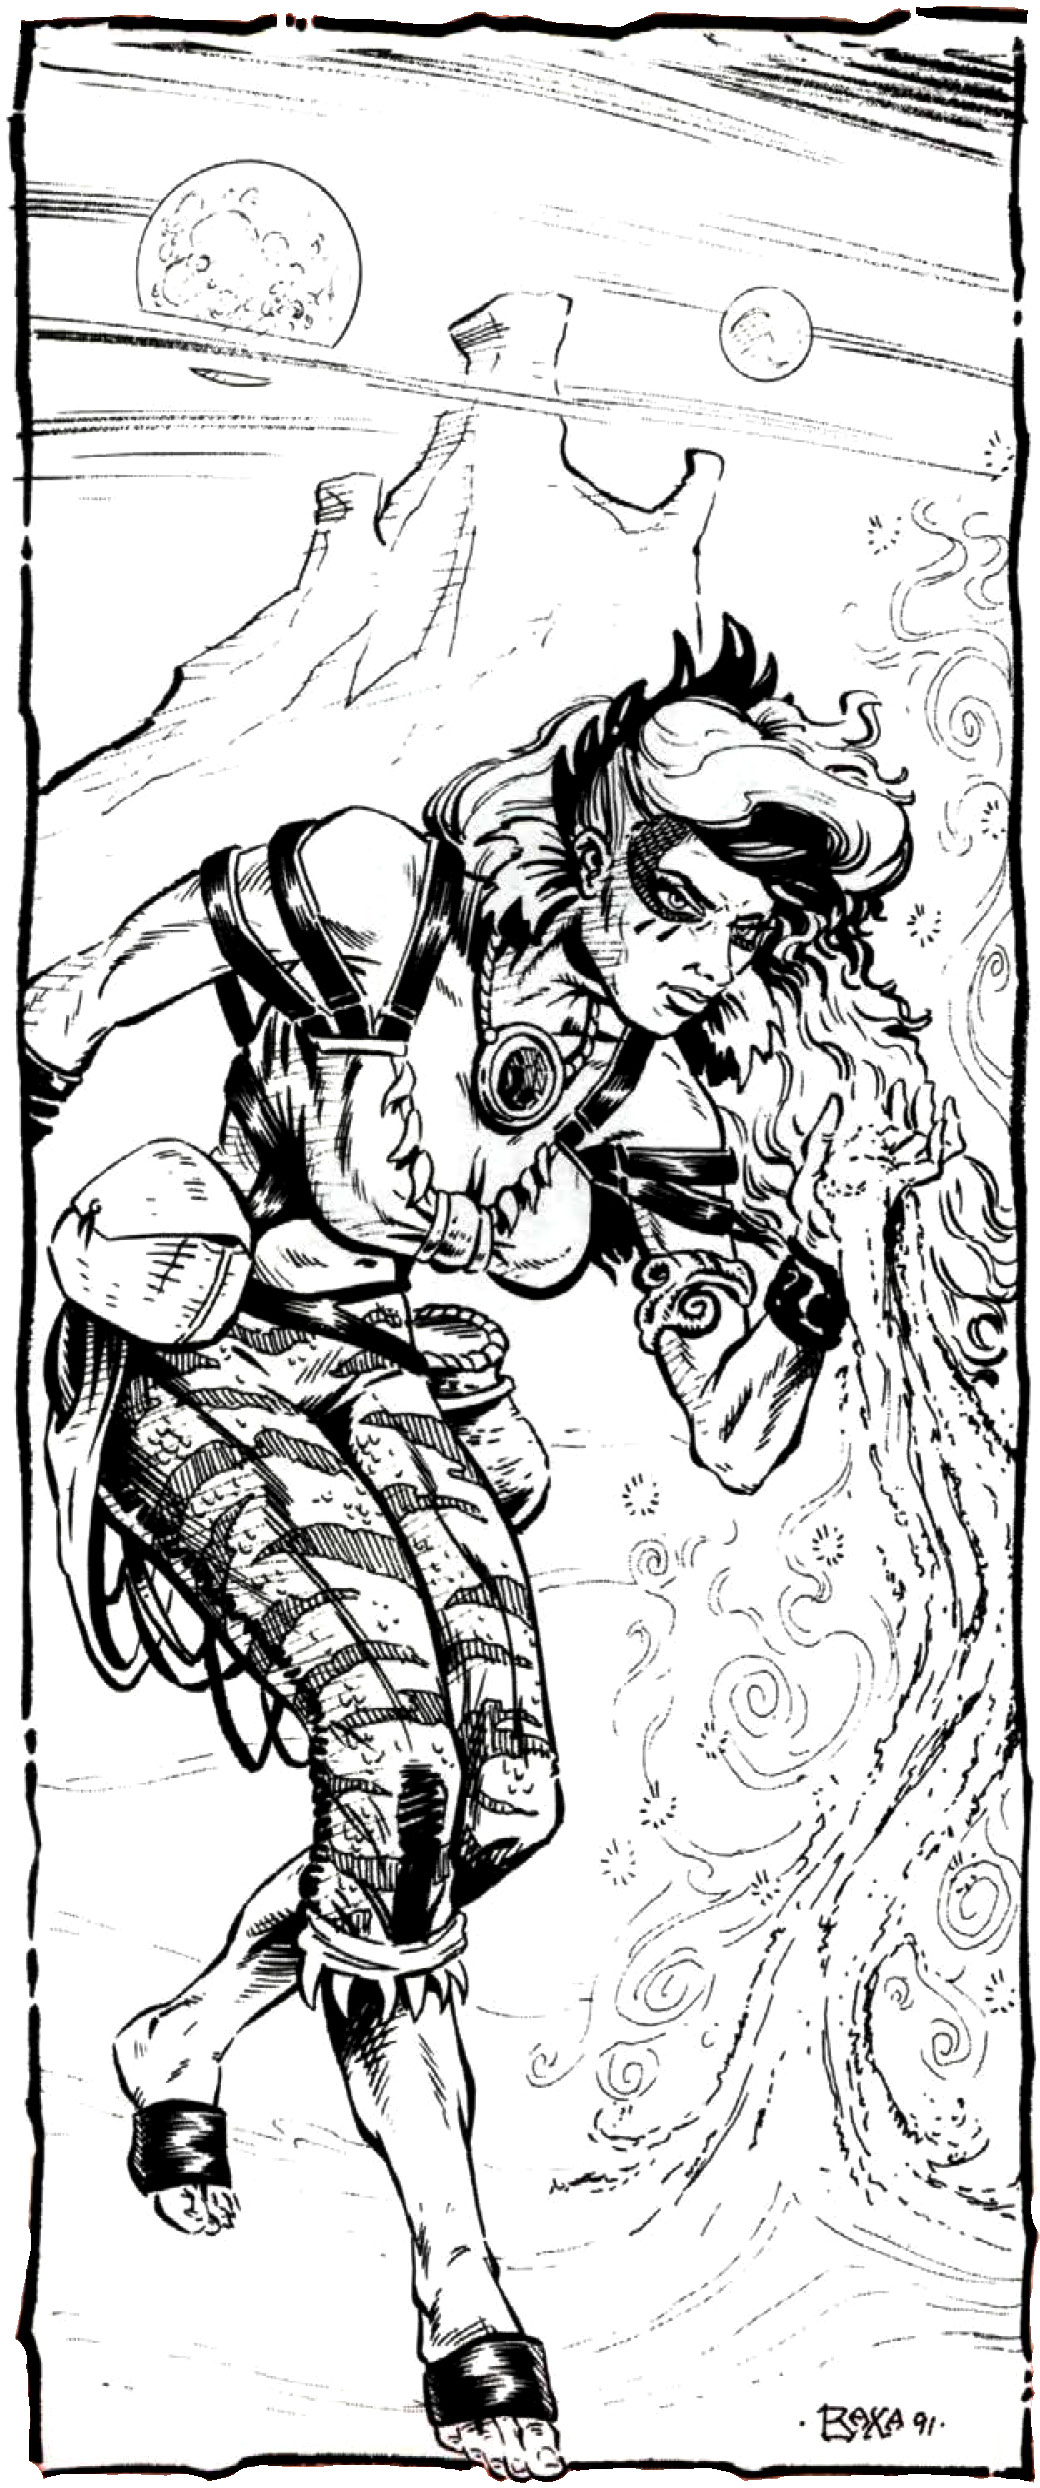
\includegraphics[width=\columnwidth]{images/wizard-2.png}
\WOTC
\end{figure}


\textbf{Abjuration:} Spells that protect, block, or banish. An abjuration specialist is called an abjurer.

\textbf{Conjuration:} Spells that bring creatures or materials to the caster. A conjuration specialist is called a conjurer.

\textbf{Divination:} Spells that reveal information. A divination specialist is called a diviner. Unlike the other specialists, a diviner must give up only one other school.

\textbf{Enchantment:} Spells that imbue the recipient with some property or grant the caster power over another being. An enchantment specialist is called an enchanter.

\textbf{Evocation:} Spells that manipulate energy or create something from nothing. An evocation specialist is called an evoker.

\textbf{Illusion:} Spells that alter perception or create false images. An illusion specialist is called an illusionist.

\textbf{Necromancy:} Spells that manipulate, create, or destroy life or life force. A necromancy specialist is called a necromancer.

\textbf{Transmutation:} Spells that transform the recipient physically or change its properties in a more subtle way. A transmutation specialist is called a transmuter.

\textbf{Universal:} Not a school, but a category for spells that all wizards can learn. A wizard cannot select universal as a specialty school or as a prohibited school. Only a limited number of spells fall into this category.

\subsubsection{Ex-Defilers}
Arcane casters who defile must roll a Will save DC 10 + spell level + amount of times previously defiled. Failing this save, they become defilers. Preservers succeeding the save lose their preserver status and become tainted. For more rules on defiling, see \chapref{Magic}.

Tainted wizards are not defilers, but risk becoming so. Tainted wizards may seek redemption from a druid. The druid, if willing and able, can cast a \spell{conversion} spell on the tainted wizard, restoring her preserver status (reset the number of times defiled to zero). The wizard loses 100 XP per arcane spellcaster level.

Defilers can also seek redemption, but lose 1,000 XP per arcane spellcaster level. Usually the defiler must undertake a quest or otherwise demonstrate a true willingness to redeem herself before the druid casts the \spell{conversion} spell.


\subsection{Playing a Wizard}
You are a master of arcane secrets. You have learned, either on your own, or from someone in your family, how to draw on vegetable life in order to power your spells. But such power comes with a caveat, arcane magic is universally feared and hated. You might be inclined to see conspiracies and enemies where none exist, so accustomed are you to being hunted and persecuted by the general populace and sorcerer-king's templars because of your talents.

Mostly, you adventure to perfect your understanding and mastery of magic. You likely prefer endeavors that allow frequent use of your abilities, or those that promise access to ancient lore. You might have personal goals as well, and it's not uncommon for an Athasian wizard to adventure for the sake of riches, power, eternal life, or any other ``standard'' adventurer motive.

\subsubsection{Religion}
Wizards frequently find themselves at odds with the elemental forces that grant clerics their powers, though it is not unheard of for preservers to forge an Elemental Pact. Some preservers might also associate themselves with the assorted Spirits of the Land. Since they understand the sorcerer-kings to simply be exceptionally advanced wizards, they are not given to revering their kings, as some of their more naive brothers are known to do.

\subsubsection{Other Classes}
Wizards have a difficult time relating to most of the other classes. Templars and wizards are, in most cases, deadly enemies across an irreconcilable gap---the exception is those rare defilers in the employ of the sorcerer-kings. Likewise, druids are likely to consider any wizard a potential defiler, and would turn on a companion the moment this suspicion is confirmed. Due to their similar, ``underground'' nature, wizards feel a certain respect for bards. While preservers enjoy an uneasy truce with the elemental powers, defilers and paraelemental clerics tend get along quite well.

\subsubsection{Combat}
Athasian wizards stay back from melee and use your spells to either destroy your enemies or enhance your companion's abilities. Secrecy is a major component, even more so if you are a defiler. Casting even of the simplest of arcane spells can focus all of your enemies' attention to you, even more so if you are a defiler. Be prepared to run of fly away in such cases.

\subsubsection{Advancement}
Continuing your advancement as a wizard requires a substantial amount of time and effort. You must procure and study arcane texts, not merely to learn new spells, but to comprehend the nature of what you do.

When you not studying, you are practicing, training your mind and your body to channel ever greater amounts of life force.

As you start to progress in the class, consider studying other sources of arcane energy, such as the Black, the Gray, and the Cerulean, since those would remove your dependency on vegetable life around you. Most wizards seek to become some day as powerful as Dragon Kings or the fabled winged creature the Urikite known as Korgunard turned into.

Mechanically, you should increase your Intelligence and Charisma as you attain levels. Beyond this, focus on feats (such as Path Dexter or Path Sinister) and skills that enhance your spells and provide you the abilities you need to remain in secrecy, mainly Bluff and Disguise.

\vskip3cm

\subsection{Starting Packages}
\subsubsection{The Dexter}
Pterran Wizard

\textbf{Ability Scores:} Str 8, Dex 10, Con 10, Int 15, Wis 16, Cha 15.

\textbf{Skills:} \skill{Bluff}, \skill{Concentration}, \skill{Disguise}, \skill{Knowledge} (arcana), \skill{Knowledge} (local), \skill{Spellcraft}.

\textbf{Languages:} Common, Elven, Saurian.

\textbf{Feat:} \feat{Path Dexter}.

\textbf{Weapons:} Dagger (1d4/19--20, 3 m)

Light crossbow with 20 bolts (1d6/$\times$3, 18 m).

\textbf{Armor:} Padded (+1 AC).

\textbf{Other Gear:} Standard adventurer's kit, spell

component pouch, 31 cp.

\subsubsection{The Concurrent}
Human Wizard

\textbf{Ability Scores:} Str 8, Dex 13, Con 10, Int 15, Wis 14, Cha 12.

\textbf{Skills:} \skill{Bluff}, \skill{Concentration}, \skill{Decipher Script}, \skill{Disguise}, \skill{Knowledge} (arcana), \skill{Knowledge} (local), \skill{Spellcraft}.

\textbf{Languages:} City language, Common, Elven.

\textbf{Feat:} \feat{Alertness}, \feat{Improved Initiative}.

\textbf{Weapons:} Dagger (1d4/19--20, 3 m)

Light crossbow with 20 bolts (1d6/$\times$3, 18 m).

\textbf{Armor:} Padded (+1 AC).

\textbf{Other Gear:} Standard adventurer's kit, spell component pouch, 31 cp.

\subsubsection{The Sinister}
Elf Wizard

\textbf{Ability Scores:} Str 10, Dex 16, Con 10, Int 15, Wis 13, Cha 8.

\textbf{Skills:} \skill{Bluff}, \skill{Concentration}, \skill{Knowledge} (arcana), \skill{Knowledge} (local), \skill{Spellcraft}.

\textbf{Languages:} City language, Common, Elven.

\textbf{Feat:} \feat{Destructive Raze}.

\textbf{Weapons:} Dagger (1d4/19--20, 3 m)

Light crossbow with 20 bolts (1d6/$\times$3, 18 m).

\textbf{Armor:} Padded (+1 AC).

\textbf{Other Gear:} Standard adventurer's kit, spell component pouch, 31 cp.

\subsection{Wizards on Athas}
\Quote{'Witch!' they chanted. 'Kill the witch!' By the time the soldiers woke, the crowd had finished her off, and worse. The mage's death did not satisfy the mob; her body suffered much more. When the mul leader shouted, 'we'll take her and burn her!' they cheered. For the only time in my life I saw a crowd cheer for Kalak's guards. For the first time I saw wizard's magic. For the first time I understood its peril.}{Manok, Tyrian wizard}

On Athas, the energy for wizardly magic doesn't come from some extradimensional source as it does on other worlds, but from the living environment itself. It provides great power to those who can gather and shape it, though the cost to Athas can be beyond measure.

In recent times wizards have emerged who have learned to draw energy from alternate sources that have no impact on the environment, see Prestige Class Appendix I for more information.

\subsubsection{Daily Life}
The kinds of activities that appeal to wizards depend largely on their alignment and energy gathering method. Good wizards spend their time trying to restore the devastation of Athas and fighting against the forces of the sorcerer-kings, while evil preservers of defilers are interested in helping themselves.

When not adventuring, Athasian wizards spend the majority of their time in study and in hiding. Much like wizards from other settings, they must constantly research new spells and study ancient arcane texts so thoroughly that they have little time to devote to other endeavors.

\subsubsection{Notables}
Usually wizards try to stay incognito for as long as they can, since their survival depends on it. However, a few wizards manage to become quite famous on Athas. Royal defilers and arena necromancers, such as Dote Mal Payn, even though hated by the general populace are sponsored by their sorcerer-kings and do not need to hide their skills. Sadira of Tyr was made famous for her contribution in killing King Kalak the Tyrant and the Dragon, and she has become the first (and maybe the only one) wizard able to tap into the power of the crimson sun. The most famous wizards are the Dragon Kings, of course, who can destroy both plant life and living creatures to power their spells.

\subsubsection{Organizations}
Wizardly magic on Athas isn't as codified and formal as it is in other campaign settings. For example, there are no academies or colleges for teaching the wizardly arts. Instead, a wizard-in-training must find a teacher, which isn't very easy in a world where wizards must hide their profession in order to survive. For protection from nearly universal hatred, the good wizards of Athas and their allies have formed secret societies, collectively known as the Veiled Alliance.

However, each city-state holds a different Alliance, they do not cooperate, and they share no leaders. Members of one Alliance do not automatically become members of another. At best, the different groups respect each other, and may offer courtesy assistance to a foreign member who arrives in town.

Defilers don't usually organize together, but they often join organizations, especially Merchant Houses and raiding tribes.

\subsubsection{NPC Reactions}
Arcane magic in Athas is viewed as more dangerous and destructive than helpful, so general NPC attitudes towards someone suspected to be a wizard range from indifferent to unfriendly. If a NPC actually witness a wizard drawing magical energy or casting a spell, the resultant fear and hatred shifts the NPC's attitude toward hostile.

Arcane magic is banned in almost all city-states; Tyr has unbanned it after FY 0 after Kalak was killed and Kurn has no qualms about preserving magic. Templars constantly patrol the streets searching for wizards and arcane items.

\subsubsection{Wizard Lore}

Characters with ranks in \skill{Knowledge} (arcana) can research wizards to learn more about them. When a character makes a skill check, read or paraphrase the following, including the information from lower DCs.

\textbf{DC 10:} Wizards are magic users that fuel their spells with plant life.

\textbf{DC 15:} A wizard can be either a defiler or a preserver. Only the first destroys the land when casting a spell. Defilers can increase the potency of their spells by destructing larger areas of vegetation than necessary.

\textbf{DC 20:} Some say that other wizards have developed a way to draw energy from other source than plants.


\begin{figure}[b!]
\centering
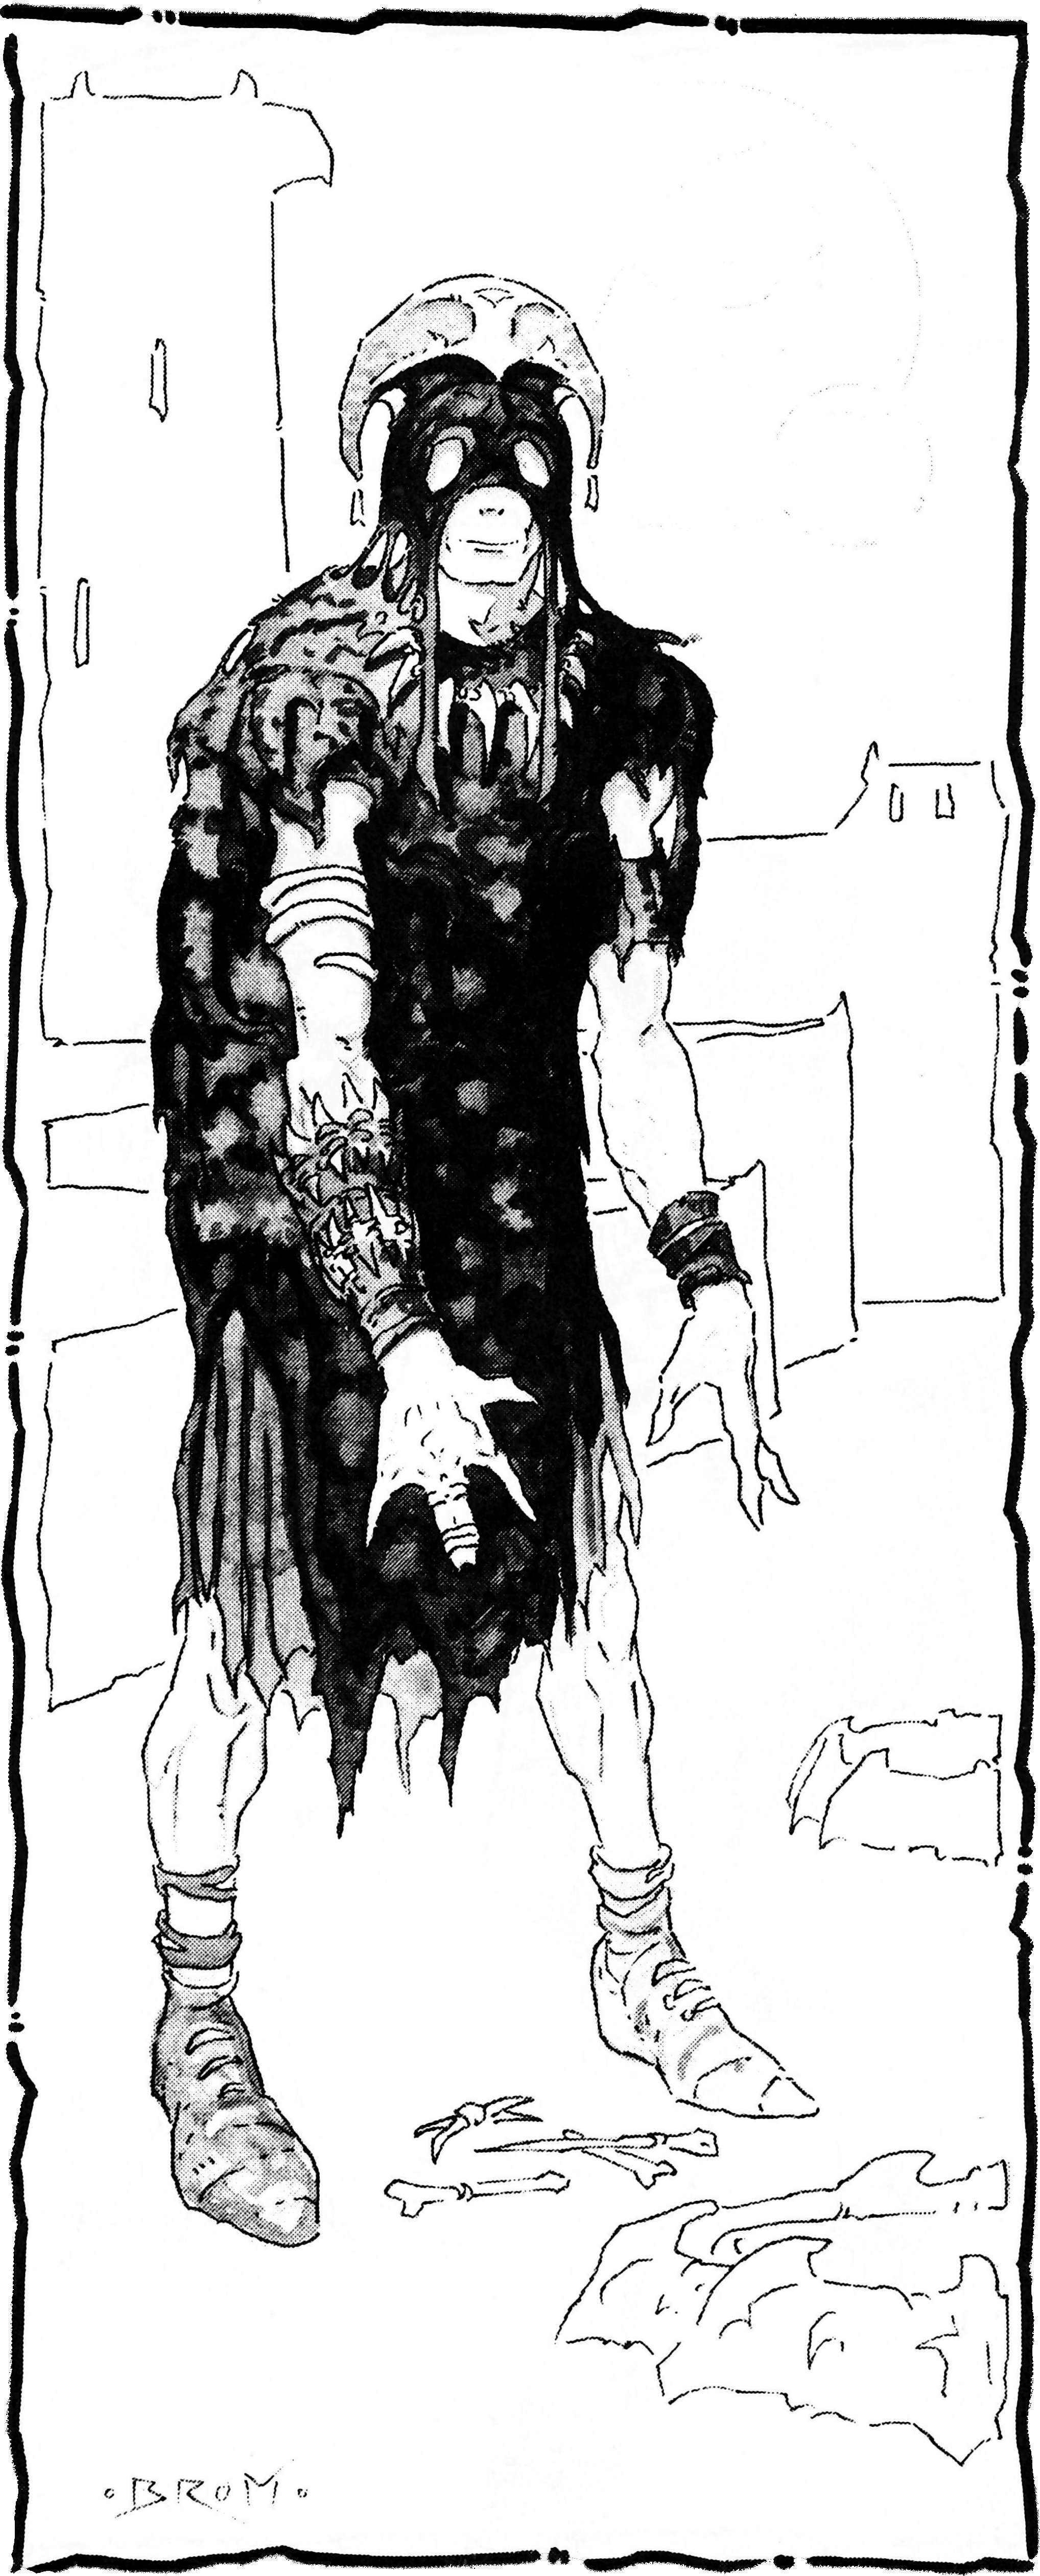
\includegraphics[width=\columnwidth]{images/wiz-1.png}
\WOTC
\end{figure}
\clearpage
\section{Character Progress}

DMs use adventures to offer a number of challenges (or encounters) for the characters to overcome. As the characters overcome these encounters, they should improve and gain new abilities to overcome greater challenges. The rate of encounters is called the pace of the adventure, or the pace of the campaign. \tabref{Paces of Campaign} shows how many encounters or sessions are expected for each type of campaign.

\Table{Paces of Campaign}{X R R}{
\tableheader Pace of Campaign & \tableheader Encounters per Level & \tableheader Sessions per Level\\
Rushed  &  5 encounters & 1 session \\
Fast    & 10 encounters & 2 sessions \\
Default & 12 encounters & 3 sessions \\
Slow    & 15 encounters & 4 sessions \\
Dragged & 20 encounters & 5+ sessions \\
}

Instead of the standard of using Experience Points (XP) to attain new character levels, we recommend that players gain levels based on a fixed number of sessions. This way the DM can tailor the experience based on the frequency of the sessions, e.g., if your group can only play once per month it may be better to speed up the progress of the characters.

If your group would rather use a traditional leveling system via XP, you can use \tabref{Traditional Experience and Wealth}. In this table there is the expected wealth of player characters. Use this as a guide to balance adventures, i.e., do not assume a 3rd-level character should have a 3,000 cp item.

\Table{Traditional Experience and Wealth}{lRRR}{
\tableheader ECL & \tableheader Total XP & \tableheader XP for next level & \tableheader Wealth\\
1  &         &  1,500 & 3d4 $\times$ 10 cp\\
2  &   1,500 &  3,000 & 600 cp\\
3  &   4,500 &  4,500 & 1,500 cp\\
4  &   9,000 &  6,000 & 3,000 cp\\
5  &  15,000 &  7,500 & 6,000 cp\\
6  &  22,500 &  9,000 & 9,000 cp\\
7  &  31,500 & 10,500 & 12,000 cp\\
8  &  42,000 & 12,000 & 18,000 cp\\
9  &  54,000 & 13,500 & 24,000 cp\\
10 &  67,500 & 15,000 & 30,000 cp\\
11 &  82,500 & 16,500 & 42,000 cp\\
12 &  99,000 & 18,000 & 54,000 cp\\
13 & 117,000 & 19,500 & 66,000 cp\\
14 & 136,500 & 21,000 & 90,000 cp\\
15 & 157,500 & 22,500 & 114,000 cp\\
16 & 180,000 & 24,000 & 138,000 cp\\
17 & 204,000 & 25,500 & 186,000 cp\\
18 & 229,500 & 27,000 & 234,000 cp\\
19 & 256,500 & 28,500 & 282,000 cp\\
20 & 285,000 &        & 378,000 cp\\
}

\subsubsection{Level-Dependent Benefits}
Besides the bonuses given by their character classes, all characters gain additional feats and increase their abilities from advancing in level as seen in \tabref{Level-Dependent Benefits}. This does not count a race's level adjustment---only character classes.

\textbf{Feat:} Every character gets their first feat at 1st level. At 3rd level and every other 3 levels, characters gain another feat. More information on feats on \chapref{Feats}.

\textbf{Ability Score Increase:} At 4th level and every 4 levels thereafter, the player chooses one of their character's ability scores to increase by 1 point. This improvement is permanent.

\textbf{Class Skill Max Ranks:} The maximum number of ranks a character can have in a class skill is equal to their character level +3.

\textbf{Cross-Class Skill Max Ranks:} For cross-class skills, the maximum number of ranks is one-half the maximum for a class skill.

\Table{Level-Dependent Benefits}{lccCC}{
\multirow[b]{2}{11mm}{\tableheader Character Level}
& \multirow[b]{2}{5mm}{\centering \tableheader Feat}
& \multirow[b]{2}{15mm}{\centering \tableheader Ability Score\\Increase}
& \multicolumn{2}{c}{\tableheader Max Ranks}\\
\cmidrule[0.5pt]{4-5}
&&& \tableheader Class Skill & \tableheader Cross-Class Skill\\

 1 & 1st &     &  4 & 2          \\
 2 &     &     &  5 & 2\onehalf  \\
 3 & 2nd &     &  6 & 3          \\
 4 &     & 1st &  7 & 3\onehalf  \\
 5 &     &     &  8 & 4          \\
 6 & 3rd &     &  9 & 4\onehalf  \\
 7 &     &     & 10 & 5          \\
 8 &     & 2nd & 11 & 5\onehalf  \\
 9 & 4th &     & 12 & 6          \\
10 &     &     & 13 & 6\onehalf  \\
11 &     &     & 14 & 7          \\
12 & 5th & 3rd & 15 & 7\onehalf  \\
13 &     &     & 16 & 8          \\
14 &     &     & 17 & 8\onehalf  \\
15 & 6th &     & 18 & 9          \\
16 &     & 4th & 19 & 9\onehalf  \\
17 &     &     & 20 & 10         \\
18 & 7th &     & 21 & 10\onehalf \\
19 &     &     & 22 & 11         \\
20 &     & 5th & 23 & 11\onehalf \\
}

\subsection{Gaining Experience}
Award players for combat, skills, and role-playing. Combat can be inevitable and emerging victorious in a combat should earn experience points. Skills are the way of dealing with problems without violence. Like combat, awards are only for successful attempts.

There are also some guidelines to award players experience points for their roleplay. These are based on their race, so that they are incentivized to follow the racial culture.

\subsubsection{Awards per Race}
These awards are for roleplaying some of the stereotypical aspects of athasian character races. Players should remember that races are more than just stats on their character sheets, they have culture and history which are what these stereotypes try to enforce.

The judgment of good roleplaying ultimately lies with the DM, and they must be familiar with the nuances of the character races. The communication between the DM and the players should be clear so that a good roleplaying experience can arise, and the nature of \textbf{Dark Sun} can be emphasized.

To determine the XP award for a particular action, check the correspondent table for the character's race and multiply the award by the character's effective character level (ECL). Remember that this will quicken the rate of progress of the characters.

\textbf{Aarakocra}: Aarakocras are claustrophobic. Whenever not entering a closed space becomes a hard choice, aarakocras should be rewarded for choosing their phobia over the closed space. This should not be awarded when the stakes for not entering are low.

Aarakocras are a flying race. Whenever aarakocras enter buildings through windows because they were flying high, they should get experience bonus.

\XPTable{Aarakocras}{
Enter building through window & 25 XP \\
Refuse to enter closed spaces & 100 XP \\
}

\textbf{Dwarf}: Dwarves live by their foci. A focus must take at least a week to complete. If a focus takes a least a year to complete, it becomes a major focus.

Focus can be changed in very rare circumstances. These circumstances must be agreed between the player and the DM.

\XPTable{Dwarves}{
Pursue present focus & 50 XP $\times$ days pursuing \\
Ignore present focus & -100 XP $\times$ days ignoring \\
Complete major focus & 1,000 XP \\
}

\textbf{Elf}: Roleplaying an elf is centered around trust. Elves are self-reliant and do not want to gain friendship with every character they meet. They test redeemable outsiders (in the elvish perspective) to see if they are trustworthy.

\textit{Examples of subtle tests of trust}:
\begin{itemize*}
	\item entrust with confidential information,
	\item leave a valuable item easy for taking to see the outsider takes it,
	\item ask to deliver a message or item.
\end{itemize*}

\textit{Examples of life-threatening tests of trust}:
\begin{itemize*}
	\item let themselves get captured to see if there is a rescue attempt,
	\item fake unconsciousness after a battle to see what type of care is provided,
	\item cut supplies to see if they get a fair share.
\end{itemize*}

\XPTable{Elves}{
Subtle test of trust & 25 XP \\
Life-threatening test of trust & 200 XP \\
Refuse animal or magical transport & 50 XP \\
Continuous run & 10 XP $\times$ distance in km \\
}

\textbf{Half-Elf}: Every half-elf seek acceptance among humans and elves, t hough they deny it as much as possible. Observing simple customs for the first time should award bonus experience points. These can be drinking the local ale with the elven chieftain or participating in a human wedding ritual.

If a local custom takes form of a competition, the half-elf gains bonus experience points if they perform better than any \emph{one} of the humans or elves also participating. If they perform better than \emph{all} the humans or elves, they get double the experience award.

\XPTable{Half-Elves}{
Observe human or elven custom & 25 XP \\
Better a human or elf in custom & 250 XP \\
}

\textbf{Half-Giant}: A half-giant seeks guidance and purpose in others' lifestyles. Player characters should seek to imitate the most charismatic member of the party in their racial and class customs. Whenever they do, they should be rewarded for it.

Half-giant can also look elsewhere for inspiration, imitating non-player characters and may even switch sides in an adventure. Whenever a player goes this far, they should get bonus experience points.

Whenever half-giants shift their alignment based on the events in the campaign, the DM should give them bonus experience points. This is only for appropriate shifts that are followed by a meaningful roleplay.

\XPTable{Half-Giants}{
Imitate charismatic friend & 25 XP $\times$ days imitating \\
Shift alignment per influence & 50 XP \\
}

\textbf{Halfling}: Halflings come from isolated tribes and, similar to half-elves, they want to experiment other races' customs. Unlike half-elves, their drive is curiosity, instead of trying to fit in. Whenever halflings try a  custom for the first time, no matter how trivial, they gain an experience bonus.

Their sense of belonging makes them honor bound to aid another halfling in need. This should only be rewarded when there is danger of injury or loss of life to the aiding halfling.

\XPTable{Halflings}{
Refuse money & 25 XP \\
Practice another race's custom & 50 XP \\
Eat slain foe & 50 XP \\
Aid another halfling & 100 XP \\
}

\textbf{Mul}: As a race bred exclusively for slavery, muls lack a culture similar to the other races. What they all share is the culture of labor. Whenever they exert themselves, they should be awarded bonus experience. This should only be rewarded if the exertion is meaningful to the adventure.

\XPTable{Muls}{
Heavy exertion & 10 XP $\times$ day of work \\
}

\textbf{Pterran}: Pterran culture venerates Earth Mother, so whenever pterrans celebrate her they should be rewarded. This also means that defilers are natural foes to pterrans, since they desecrate Earth Mother.

As a vibrant culture, they are curious to witness other cultures---as long as they don't harm the Earth Mother.

\XPTable{Pterrans}{
Celebration for Earth Mother & 25 XP\\
Practice another race's custom & 50 XP \\
Defeat defiler & 50 XP $\times$ defiler's CR\\
}

\textbf{Thri-Kreen}: Thri-kreen come from an empire of hunter-gatherers. Whenever they take back a slain creature for food, it should warrant experience bonus.

\XPTable{Thri-Kreens}{
Defeat creature for food & 50 XP \\
Paralyze creature & 100 XP \\
}

% \subsubsection{Awards per Class}
% Multiclass characters must choose which class to consider when receiving awards---you can only gain award for a single class.

% \textbf{\class{Barbarian}}: Barbarians are survivalists, so beyond defeating living creatures, defeating traps and natural hazards on their might alone award them bonus experience points.

% \XPTable{Barbarians}{
% Use special attack & 5 XP\\
% Use rage & 10 XP\\
% Defeat a creature & 10 XP $\times$ creature's CR\\
% Defeat trap or natural hazard & 10 XP $\times$ trap's CR\\
% }

% \textbf{\class{Bard}}: Bards gain bonus experience points for successful use of their bardic abilities. However they also gain XP for using poison against a creature---to weaken or kill the victim.

% \XPTable{Bards}{
% Use bardic music & 10 XP\\
% Use bardic knowledge & 25 XP\\
% Use poison effectively & 5 XP $\times$ creature's CR\\
% Defeat a creature & 5 XP $\times$ creature's CR\\
% Obtain treasure & 5 XP $\times$ value in cp\\
% }

% \textbf{\class{Cleric}}: Using elements with finesse and flair to overcome an obstacle should reaward clerics bonus experience points.

% \XPTable{Clerics}{
% Use domain power & 10 XP\\
% Use element creatively & 50 XP\\
% Cast spell & 5 XP $\times$ spell level\\
% Cast Healing spell & 10 XP $\times$ spell level\\
% Turn/rebuke undead & 25 XP $\times$ undead's CR\\
% Destroy/command undead & 50 XP $\times$ undead's CR\\
% Create magic item & 200 XP\\
% }

% \textbf{\class{Druid}}:

% \XPTable{Druids}{
% Cast spell & 5 XP $\times$ spell level\\
% Case Healing spell & 10 XP $\times$ spell level\\
% Use wild empathy & 25 XP\\
% Use wild shape & 10 XP\\
% Defeat defiler & 50 XP $\times$ defiler's CR\\
% Create magic item & 200 XP\\
% }

% \textbf{\class{Fighter}}: The fighter's role in society is about mass warfare, so being a good soldier during these times will award her additional experience points. Fighters do not gain experience points for spending weeks in reserve, even if they're commanding followers.

% \XPTable{Fighters}{
% Use special attack & 5 XP\\
% Defeat a creature alone & 5 XP $\times$ creature's CR\\
% Defeat a creature with a group & 10 XP $\times$ creature's CR\\
% Follow commands in battle & 25 XP\\
% Command a battle & 50 XP\\
% Build a war machine & 100 XP\\
% }

% \textbf{\class{Gladiator}}: Gladiators desire to be in the spotlight of an arena, to be the victor of a duel. Therefore, they receive additional experience points for defeating creatures in an arena without outside aid. The glory must be their alone.

% \XPTable{Gladiators}{
% Use special attack & 5 XP\\
% Use gladiatorial perfomance & 10 XP\\
% Defeat a creature & 5 XP $\times$ creature's CR\\
% Defeat a creature alone in an arena & 10 XP $\times$ creature's CR\\
% }

% \textbf{\class{Psion}}:

% \XPTable{Psions}{
% Defeat a psionic creature & 5 XP $\times$ creature's CR\\
% Research new psionic knowledge & 50 XP\\
% Manifest a power & 5 XP $\times$ power level\\
% Manifest a power to avoid combat & 10 XP $\times$ power level\\
% Create psionic item & 200 XP\\
% }

% \textbf{\class{Psychic Warrior}}:

% \XPTable{Psychic Warriors}{
% Defeat a creature & 5 XP $\times$ creature's CR\\
% Defeat a psionic creature & 5 XP $\times$ creature's CR\\
% Manifest a power & 5 XP $\times$ power level\\
% }

% \textbf{\class{Ranger}}: Rangers track their foes and hunt favored enemies. Accomplishing these taks award them additional experience points.

% \XPTable{Ranger}{
% Cast spell & 5 XP $\times$ spell level\\
% Defeat a creature & 5 XP $\times$ creature's CR\\
% Defeat a creature in a favorite territory & 5 XP $\times$ creature's CR\\
% Defeat a favorite enemy & 10 XP $\times$ enemy's CR\\
% Track a creature & 10 XP\\
% Track a creature in a favorite territory & 10 XP\\
% Track a favorite enemy & 10 XP\\
% Use wild empathy & 25 XP\\
% }

% \textbf{\class{Rogue}}:

% \XPTable{Rogue}{
% Defeat a creature & 5 XP $\times$ creature's CR\\
% Disable trap & 25 XP $\times$ trap's CR\\
% Obtain treasure & 5 XP $\times$ value in cp\\
% Obtain treasure for patron & 5 XP $\times$ value in cp\\
% Use sneak attack & 5 XP\\
% }

% \textbf{\class{Templar}}:

% \XPTable{Templar}{
% Cast spell & 5 XP $\times$ spell level\\
% Use secular authority on slave & 5 XP\\
% Use secular authority on freeman & 10 XP\\
% Use secular authority on noble & 25 XP\\
% Use secular authority on templar & 50 XP\\
% Fulfill sorcerer-king's mission & 100 XP\\
% }

% \textbf{\class{Wilder}}:

% \XPTable{Wilders}{
% Defeat a psionic creature & 5 XP $\times$ creature's CR\\
% Create psionic item & 200 XP\\
% Surge without enervation & 10 XP $\times$ bonus level\\
% Manifest a power & 5 XP $\times$ power level\\
% Manifest a power to avoid combat & 10 XP $\times$ power level\\
% }

% \textbf{\class{Wizard}}: Preservers and defilers serve different roles in the athasian society. Preservers want to remain hidden from the eyes of the templars, so they gain additional experience points for keeping spellcasting secret. Defilers on the other hand are aligned with the \emph{status quo} and are awarded additional experience points for carrying out the business of their sorcerer-monarchs.

% \XPTable{Wizards}{
% Cast spell & 5 XP $\times$ spell level\\
% Cast spell for sorcerer-king (defiler) & 5 XP $\times$ spell level\\
% Find new spell to spellbook & 50 XP $\times$ spell level\\
% Keep spellcasting secret (preserver) & 25 XP\\
% Create magic item & 200 XP\\
% }

\subsubsection{Awards for Skill Check}
Skill checks represent nonviolent challenges in the game. To determine the XP award for a successful skill check, follow these steps:

\begin{enumerate*}
	\item Calculate the adjusted Difficulty Class (DC) of the check. It is equal to the skill check's DC minus any racial bonus the character has in that check.
	\item Use \tabref{Experience Awards from Skill Checks} to cross-reference the campaign's pace with the adjusted DC to find the XP award.
\end{enumerate*}
 
Only successful checks award XP. Checks with adjusted DC lower than 10 do not give XP. The award is not based on the check's result.

Opposed checks do not have Difficulty Class. For the purposes of experience awards, they are considered to have a DC equal to a roll of 12. For example, a barbarian with a Hide modifier of +4 would be awarded 50 XP if they pass a Hide check DC 16---regardless of the result of the barbarian's Hide check or any opposed Spot check.

\Table{Experience Awards from Skill Checks}{L *5C}{
\rowcolor{white}
\multirow[c]{2}{1cm}{\tableheader Adjusted DC} & \multicolumn{5}{c}{\tableheader Experience Points Award}\\
\cmidrule[0.5pt]{2-6}
& \tableheader Rushed & \tableheader Fast & \tableheader Normal & \tableheader Slow & \tableheader Dragged \\

10--11 & 25 & 15 & 10 & 8 & 5 \\
12--14 & 60 & 30 & 25 & 20 & 15 \\
15--19 & 120 & 60 & 50 & 40 & 30 \\
20--24 & 250 & 120 & 100 & 80 & 60 \\
25--29 & 600 & 300 & 250 & 200 & 150 \\
30--39 & 1,200 & 600 & 500 & 400 & 300 \\
40--49 & 2,400 & 1,200 & 1,000 & 800 & 600 \\
50+ & 6,000 & 3,000 & 2,500 & 2,000 & 1,500 \\
}

\subsubsection{Awards for Combat}
When the players defeat the enemy in battle, they earn experience points. Only characters who take part in the battle should gain XP. Characters who died before the combat, or did not participate for any other reason, should not be awarded.

To determine the XP award for a combat, follow these steps.
\begin{enumerate*}
	\item Determine each character's effective character level (ECL).
	\item For each monster or trap defeated, determine its Challenge Rating (CR).
	\item Use \tabref{Experience Awards from Combats} to cross-reference the campaign's pace with the CR of each monster or trap to find the base XP award.
	\item Divide the base XP award by the number of characters in the party.
	\item Add up all the XP awards for all the monsters or traps the character helped defeat.
	\item Repeat the process for each character.
\end{enumerate*}

Creatures summoned or that otherwise are related to an enemy's ability (such as animal companion) do not award XP. These abilities are already taken into account in the enemy's CR.

\Table{Experience Awards from Combats}{X *{5}{C}} {
\rowcolor{white}
\multirow[l]{2}{1cm}{\tableheader Challenge Rating} & \multicolumn{5}{c}{\tableheader Experience Points Award (per monster)}\\
\cmidrule[0.5pt]{2-6}
& \tableheader Rushed & \tableheader Fast & \tableheader Normal & \tableheader Slow & \tableheader Dragged \\

1 & 1,200 & 600 & 500 & 400 & 300 \\
2 & 2,400 & 1,200 & 1,000 & 800 & 600 \\
3 & 3,600 & 1,800 & 1,500 & 1,200 & 900 \\
4 & 4,800 & 2,400 & 2,000 & 1,600 & 1,200 \\
5 & 6,000 & 3,000 & 2,500 & 2,000 & 1,500 \\
6 & 7,200 & 3,600 & 3,000 & 2,400 & 1,800 \\
7 & 8,400 & 4,200 & 3,500 & 2,800 & 2,100 \\
8 & 9,600 & 4,800 & 4,000 & 3,200 & 2,400 \\
9 & 10,800 & 5,400 & 4,500 & 3,600 & 2,700 \\
10 & 12,000 & 6,000 & 5,000 & 4,000 & 3,000 \\
11 & 13,200 & 6,600 & 5,500 & 4,400 & 3,300 \\
12 & 14,400 & 7,200 & 6,000 & 4,800 & 3,600 \\
13 & 15,600 & 7,800 & 6,500 & 5,200 & 3,900 \\
14 & 16,800 & 8,400 & 7,000 & 5,600 & 4,200 \\
15 & 18,000 & 9,000 & 7,500 & 6,000 & 4,500 \\
16 & 19,200 & 9,600 & 8,000 & 6,400 & 4,800 \\
17 & 20,400 & 10,200 & 8,500 & 6,800 & 5,100 \\
18 & 21,600 & 10,800 & 9,000 & 7,200 & 5,400 \\
19 & 22,800 & 11,400 & 9,500 & 7,600 & 5,700 \\
20 & 24,000 & 12,000 & 10,000 & 8,000 & 6,000 \\
}

\subsection{Alternative Progress}
Here are presented two alternative ways to change the experience progress in your campaign: partial progression and tiered powers. Each variant rule tries to delay (or halt) level progress. You are not required to use any of those variant rules to run a {\tableheader Dark Sun} adventure, since these are designed to tackle different problems and different tastes.

\subsubsection{Partial Progression}
Characters gain experience and that experience may be represented as a new level. But that is not the only way to mark character growth. Here we present some alternate rules for expending experience points. These options may be adequate for adventures that don't strive to get into high levels. Maybe you want for the characters to stay in the same level for longer than normal. With these options, they can get meaningful progression without receiving an actual level.

In \tabref{Partial Progression}, you can see the benefits and their costs. Some benefits are intentionally left out of the table, such as general feats or extra spell slots. Those benefits are too close to a new level, so it would be more meaningful to give an actual level.

\Table{Partial Progression}{XX}{
\tableheader Benefit & \tableheader XP Cost (per ECL)\\
1 skill point        & 100 XP\\
1 skill feat         & 200 XP\\
1 racial feat        & 300 XP\\
1 regional feat      & 300 XP\\
1 item creation feat & 500 XP\\
}

\textbf{Skill Point:} You gain one skill point, just as the skill points gained by acquiring a new level. You can't have more ranks than you are allowed for your level. Spending this skill point on a cross-class skill still gets your character \onehalf rank in that skill. For more information on skill points, see \chapref{Skills}.

\textbf{Feats:} You may purchase a new feat, granted you have its prerequisites. You can only purchase some types of feats: item creation feats, racial feats, regional feats, and skill feats. For more information on these types of feats, see \chapref{Feats}.

\subsubsection{Tiered Powers}
There is a natural imbalance towards magical (and psionic) powers. So much so that the whole system is balanced around wonderous items, and it is expected to have spellcasters in an adventuring group. But at higher levels, this imbalance in power can become frustrating for both DMs and players, as the powers become increasingly more complex and game-changing.

In \tabref{Tiered Powers}, you can see the level adjustment based on the maximum spell level or power level available for a manifester or spellcaster. This means that a 17th-level human wizard should be equivalent to a 19th-level character---she has access to 9th-level magic and thus has a +2 level adjustment. An elf psychic warrior of the same level (17th) should be equivalent to a 18th-level character---6th-level psionic powers grant +1 level adjustment.

\Table{Tiered Powers}{lXc}{
\tableheader Tier & \tableheader Maximum Spell/Power Level Available & \tableheader Total Level Adjustment \\
I   & 1st--3rd & +0 \\
II  & 4th--6th & +1 \\
III & 7th--9th & +2 \\
}

In an already running adventure, a character that will change their tier should only advance another level after gaining enough experience for two whole levels. For instance, Jozan is a 6th-level human cleric. In order for him to get his 7th level (and 4th-level spells), he must gain enough XP to advance to an effective 8th character level. Once the character makes a tier breakthrough, he advances normally with his level adjustment and new effective character level until another breakthrough must be made. So from his 7th level to 12th level, Jozan advances with a +1 level adjustment. After he becomes a 12th-level cleric (13 ECL), he should again acquire enough XP to advance two character levels in order to gain access to 7th-level spells---this time to an effective 15th character level. After that, he advances normally again with his +2 level adjustment.
\section{Multiclass Characters}
A character may add new classes as he or she progresses in level, thus becoming a multiclass character. The class abilities from a character's different classes combine to determine a multiclass character's overall abilities. Multiclassing improves a character's versatility at the expense of focus.

\subsection{Prerequisites}
To qualify for a new class, you must meet the ability score prerequisites for both your current class and your new one, as shown in \tabref{Multiclassing Prerequisites}. For example, a barbarian who decides to multiclass into the druid class must have Wisdom score of 15 or higher, and both Strength and Constitution scores of 13 or higher. Without the full training that a beginning character receives, you must be a quick study in your new class, having a natural aptitude that is reflected by higher-than-average ability scores.

\Table{Multiclassing Prerequisites}{lL}{
\tableheader Class & \tableheader Ability Score Minimum \\
Barbarian       & Strength 13, Constitution 13 \\
Bard            & Charisma 13, Dexterity or Intelligence 13 \\
Cleric          & Wisdom 13, Charisma 13 \\
Druid           & Wisdom 15 \\
Fighter         & Constitution 13, Strength or Dexterity 13 \\
Gladiator       & Strength 13, Intelligence or Charisma 13 \\
Psion           & Wisdom 13, Constitution or Intelligence 13 \\
% Psychic Warrior & Strength or Dexterity 13, Wisdom 13 \\
Ranger          & Wisdom 13, Strength or Dexterity 13 \\
Scout           & Dexterity 13, Strength or Wisdom 13 \\
Templar         & Wisdom 13, Charisma 13 \\
Thief           & Dexterity 13, Intelligence or Charisma 13 \\
% Wilder          & Charisma 15 \\
Wizard          & Intelligence 15 \\
}

\subsection{Class And Level Features}
As a general rule, the abilities of a multiclass character are the sum of the abilities of each of the character's classes.

\textbf{Level:} ``Character level'' is a character's total number of levels. It is used to determine when feats and ability score boosts are gained.

``Class level'' is a character's level in a particular class. For a character whose levels are all in the same class, character level and class level are the same.

\textbf{Hit Points:} A character gains hit points from each class as his or her class level increases, adding the new hit points to the previous total.

\textbf{Base Attack Bonus:} Add the base attack bonuses acquired for each class to get the character's base attack bonus. A resulting value of +6 or higher provides the character with multiple attacks.

\textbf{Saving Throws:} Add the base save bonuses for each class together.

\textbf{Skills:} If a skill is a class skill for any of a multiclass character's classes, then character level determines a skill's maximum rank. (The maximum rank for a class skill is 3 + character level.)

If a skill is not a class skill for any of a multiclass character's classes, the maximum rank for that skill is one-half the maximum for a class skill.

\textbf{Class Features:} A multiclass character gets all the class features of all his or her classes but must also suffer the consequences of the special restrictions of all his or her classes.

In the special case of turning undead, both clerics and experienced templars have the same ability. If the character's templar level is 4th or higher, her effective turning level is her cleric level plus her templar level.

In the special case of uncanny dodge, experienced barbarians, experienced gladiators, experienced scouts, and experienced thieves have the same ability. When a barbarian/rogue would gain uncanny dodge a second time (for her second class), she instead gains improved uncanny dodge, if she does not already have it. Her barbarian and rogue levels stack to determine the rogue level an attacker needs to flank her.

\textbf{Feats:} A multiclass character gains feats based on character levels, regardless of individual class level

\textbf{Ability Increases:} A multiclass character gains ability score increases based on character level, regardless of individual class level.

\textbf{Spells:} The character gains spells from all of his or her spellcasting classes and keeps a separate spell list for each class. If a spell's effect is based on the class level of the caster, the player must keep track of which class's spell list the character is casting the spell from.

\textbf{Power Points:} If you have levels in more than one psionic class, you combine your power points from each class to make up your reserve. You can use these power points to manifest powers from any psionic class you have.

While you maintain a single reserve of power points from your class, race, and feat selections, you are still limited by the manifester level you have achieved with each power you know.

\section{Contacts}
\label{sec:contacts}
This system codifies a phenomenon commonplace in most long-term campaigns: the friendly bartender, gruff weaponsmith, or absentminded sage who points the PCs in the right direction, passes along important clues, or offers unusual skills and knowledge.

Some alternate class features and prestige classes grant a PC with a reliable contact to call when the time comes. The player defines his contact at the time he gains this ability: where she lives, her race, personality, and so on. He is encouraged to roll the background of his contact (see \chapref{Character Description}).

\subsection{NPCs and Contacts}
While all defined contacts are friendly NPCs, that doesn't mean that all friendly NPCs are defined contacts. The contact mechanic is intended to supplement, not replace, other social interactions with noncombatant NPCs. It gives a player a chance to insert a minor character into the ongoing drama.

Defined contacts should be among the campaign's most stable characters. Unless the characters are completely obtuse or have remarkable misfortune, the minor characters they define as contacts aren't going anywhere. They're generally available wherever they happen to live, and they usually have the time and inclination to help their friend the PC. Major NPC characters---those defined entirely by the GM---are off limits as contacts. A player can't just say, ``I want to define the sorcerer-queen as a contact.''

A contact won't risk life or livelihood on the PC's say-so, but a contact makes some sacrifices for a friend. For example, a contact will burn the midnight oil translating an ancient text or sneak the key to the pantry out of the castle (as long as it's back by morning).

\subsection{Types of Contacts}
While your contact is friendly and tries to be helpful in small ways, you can ask for a more serious favor once per week per contact. Contacts have half as many character levels as you do. Contacts always have levels on NPC classes (see \chapref{Campaigns}). They come in three varieties, one of which you must choose: influence contacts, skill contacts, and trade contacts.

\textit{Influence Contacts:} An influence contact is an aristocrat associated with one of the big organizations of Athas (see \chapref{Organizations}). While a player can't define the leader of an organization as his character's contact, he can define one of the nobles associated with its logistic as a contact. The noble doesn't have a broad store of information, and she doesn't have any skills the PCs might need. But she might be able to put in a good word with the organization, and she can certainly make introductions between the PC and the rest of the organization's logistic staff. The purpose of an influence contact is to enable and smooth talks with more important, but less friendly, NPCs.

These contacts are not skillful nor have goods to trade, but they can pull some strings to help you in the following ways: 

\begin{itemize*}
\item Grant an appointment or meeting with an NPC (templar, noble, gladiatorial slave, chieftain, etc. At DM's discretion).
\item Access to a place to stay hidden for three days.
\item Avoid templar inspection.
\end{itemize*}

These are not the only ways an influence contact may help, but they give a direction for the DM to come up with other favors this contact can make.

\textit{Skill Contacts:} A skill contact is an expert focused on a single skill. Some skills---especially categories of \skill{Craft}, \skill{Profession}, and \skill{Knowledge}---are rarely possessed by PCs. Skill contacts have those skills in abundance, so they're useful when characters need a smith to repair a lance or an honest broker to appraise a giant emerald. Some just have an uncanny sense of what’s going on in their neighborhood or town, such as the grumpy bartender or the talkative fruit merchant. These are specialized in \skill{Diplomacy}, \skill{Gather Information}, or \skill{Sense Motive}.

This contact has maximum ranks in the skill he is best at, and his highest ability score is in the key ability for the skill in question. A skill contact always has the \feat{Skill Focus} feat related to his field of specialty. When called for a favor this contact can deliver the effect of a skill check of DC equal to 18 + \onehalf your character level.

\textit{Trade Contacts:} A trade contact is an expert who has access to a particular type of service or product. A guy who knows where to buy from the black market, or who has mercenary contacts. Whenever a barter may happen in his neighborhood, he knows. When asked for a favor, a trader contact can give you one of the following options:

\begin{itemize*}
\item +5 circumstance bonus on \skill{Diplomacy} check to bargain a single transaction.
\item Access to purchase and sell black market goods.
\item Access to hire mercenary of trader's desired race and class (see Hirelings).
\item Access to purchasing spellcasting services from a particular class.
\end{itemize*}
\section{Alternative Class Features}
Choosing a class fixes key aspects of a character: their role, their abilities, and their attack and save bonuses. However, you can change a class feature to provide a new experience. Variant versions of several of class features are presented below. If you prefer the variant to the standard class feature, ask your game master if he approves of your swapping out your class feature for the variant version.

These alternative class features can exist side by side with the standard class features---some bards might work alone while their comrades favor having contacts all over Athas---or can completely replace the standard features. The balance between the standard class features and the alternative features is up to the game master.

The description of alternative class features is the following.

\subsubsection{Alternative Class Feature Name}
A general description of the ability.

\textbf{Special Requirement:} Any special requirements that you must meet before selecting the alternative class feature. Many of the alternative class features described here require ranks of a skill. Since skill ranks are purchased before class features are selected, you can meet this requirement at the same level that you gain the alternative class feature.

\textbf{Level:} The alternative class feature can be selected only at this level. In some cases, different levels might be given for different classes.

\textbf{Replaces:} The ability that you must sacrifice to gain the alternative class feature.

\textbf{Benefit:} The mechanical effects of the new ability.


\subsection{Bard}
Athasian bards are city guides, traders, translators, or even assassins. They fill their role in society with their social skills and scoundrel minds.

\AlternateClassFeature{Contact}
{Instead of relying on their own wits like a traditional bard, a \emph{draqoman} relies on the help of others more capable in specific matters. Draqomen serve as guides and translators for newcomers to the cities. Local laws and customs vary by location, and a local resident who knows the city like the back of his hand and can call in a favor if necessary is definitely worth his pay. A draqoman will usually be loyal as long as he is paid and fed well. Mistreat your draqoman and you will soon find yourself on the wrong end of someone's blade or in the prisons run by the templars.}
{\skill{Diplomacy} 2 ranks, \skill{Gather Information} 4 ranks, \skill{Knowledge} (local) 4 ranks.}
{6th, 11th, and 16th.}
{You do not gain quick thinking, or its improvements at 11th and 16th levels.}
{
	You gain the trust of two non-player characters he can rely on when the time comes. You can ask for a favor once per week per contact. Contacts come in three varieties, one of which you must choose: influence contacts, skill contacts, and trade contacts (see \hyperref[sec:contacts]{Contacts}).

	You gain one additional contact every three levels thereafter (3 at 9th, 4 at 12th, 5 at 15th, and 6 at 18th level).
}
\AlternateClassFeature{Procurer}
{To all outward appearances, procurers seem to be everyday elf traders. They conduct their thefts in secret, using normal trading practices to cover their filching activities. These elves usually work for elven merchant houses, filling the market stalls with goods stolen from other merchants, nobles, free citizens, templars, and even the sorcerer-kings.}
{Elf or half-elf.}
{4th, 8th, 12th, 16th, or 20th.}
{You do not gain a trade secret.}
{
	You gain +5 in \skill{Search} checks to find secret doors, and if you pass within 1.5 meter of a secret door, you are entitled to a \skill{Search} check to notice it as if the character was actively looking for it.
}


\subsection{Fighter}
The nomad elves need fighters who can keep up with the tribe, maybe even lead it one day, while The Kreen Empire breeds a stronger strain to defend it against the humanoid threat. No matter the reason, Each culture and race has reached a way to specialize their fighters to survive the dangers of Athas.

\AlternateClassFeature{Reckless}
{The eagle knights are among the most brutal and fanatical Draji warriors. They are more than willing to charge headfirst into battle for the glory of Draj and their god-king.}
{Must be trained by the Draji army.}
{11th.}
{You do not gain martial prowess.}
{
	When using the attack or full attack option, you can subtract a number from his Armor Class and add this number to damage inflicted on successful attacks. This number may not exceed your base attack bonus. The Armor Class penalty and damage bonus last until the your next standard action.
}
\AlternateClassFeature{Savage Hunter}
{The savage hunter is the most common elf warrior type, serving as both a tribal defender and an important food provider. Respected by others of the tribe, the savage hunter uses the same skills to hunt prey and to fight outsiders and other threats to the tribe. The ways of the city-states are alien to these wilderness warriors, for they are only at home in the wastes when on a hunt.}
{Elf or half-elf.}
{1st.}
{You do not gain a bonus feat.}
{
	You gain \feat{Track} as a bonus feat. You add \skill{Survival} to your fighter class skills.
}

\AlternateClassFeature{Tik-Tik}
{Larger and less dexterous than most other kreen, the ``hunter-of-hunters'' guards the weaker members of the pack. In dangerous territory, Tik-Tik rarely hunt, unless the pack's normal hunters are spread too thinly or have been incapacitated by enemies.}
{Thri-kreen.}
{1st.}
{You do not gain a bonus feat.}
{
	Your natural armor bonus increases by 1 (+3 total). You add \skill{Survival} to your fighter class skills.
}


\subsection{Gladiator}
The city-state arenas are packed with all kinds of gladiators, from those who fight only with the heaviest piece of armor available to those who are able to optimize their flexibility and movement with what they have.

\AlternateClassFeature{Flexibility Adjustment}
{These gladiators adjust their armor to improve their reflex capabilities instead of increasing the area it protects.}
{}
{5th, 10th, 15th, and 20th.}
{You do not gain armor optimization, or its improvements at 10th, 15th, and 20th levels.}
{
	You improve the maximum Dexterity bonus and reduce the armor check penalty by 1, whenever you are wearing any armor you are proficient with.

	At every five levels thereafter, the improvement increases by 1 (2 at 10th, 3 at 15th, and 4 at 20th level).
}
\AlternateClassFeature{Lighten Load}
{By changing slightly the armor to their own bodies, these gladiators can move faster with a heavier armor.}
{}
{5th.}
{You do not gain the first armor optimization.}
{
	You treat the medium armor as light armor. You also reduce the armor check penalty by 1, whenever you are wearing any armor you are proficient with.
}


\subsection{Psion}
The Way is taught differently throughout the Tablelands. Urban folk teach, willingly or not, about having a friendship network in their cities. Tribal people, without formal study, have devised a ritual to aid their psychic abilities. The Kreen uses their Will to overcome the difference between their mind and the humanoid ones.

\AlternateClassFeature{Contact}
{The cities of Athas are filled with intrigue, treachery, and double-dealing. In this setting, information is a weapon that may be wielded against one's enemies. The auditor's job description ranges from information broker to psionic assassin. In most cities, the templars have auditors working for them. Other auditors are members of the Veiled Alliance, criminal gangs, or are employed by the merchant dynasties.}
{\skill{Diplomacy} 2 ranks, \skill{Gather Information} 4 ranks, \skill{Knowledge} (local) 4 ranks.}
{1st, 5th, 10th, 15th, and 20th.}
{You do not gain any bonus feat.}
{
	You gain the trust of a non-player character he can rely on when the time comes. You can ask for a favor once per week per contact. Contacts come in three varieties, one of which you must choose: influence contacts, skill contacts, and trade contacts (see \hyperref[sec:contacts]{Contacts}).

	You gain one additional use of contact at 5th level and every four levels thereafter (2 contacts at 5th, 3 at 9th, 4 at 13th, 5 at 17th).
}
\AlternateClassFeature{Psionic Ritual}
{Bereft of formal training in the Way, psionically talented individuals from the tribal and nomadic peoples of the Tablelands and beyond must make do with their own understanding of the psionic arts. Seen by formally trained psions as an aberration of proper psionic practice, these self trained individuals can sometimes produce effects that leave their detractors speechless.}
{\skill{Profession} (herbalist) 8 ranks, \skill{Survival} 6 ranks.}
{10th.}
{You do not gain a bonus feat.}
{
	Once per day, you can perform such a ritual to temporarily increase your Will. Each psionic ritual is unique, being of your own design, but all take one hour to complete and require a DC 20 \skill{Concentration} check. If the ritual is successful, you gain 1d4+1 temporary power points over and above your normal maximum. These power points remain available for one day or until they are used.
}

\AlternateClassFeature{Tekchakak}
{The tekchakak is devoted to the preservation and prosperity of clutch and pack. These psions use their abilities to support their clutchmates and packmates, helping to find prey and to defend compatriots against raiders and predators. Within a thri-kreen pack, the tekchakak offers advice, guidance, and teaching in addition to active support through their psionic abilities.}
{Thri-kreen.}
{1st.}
{You do not gain a bonus feat.}
{
	You no longer have alien mind (see \chapref{Character Races}). You add \skill{Survival} to your psion class skills.
}


\subsection{Ranger}
Protectors of the wastelands, rangers are lone survivalists who help those in need. More often than not, they aim their hatred towards those who threaten their tribes.

\AlternateClassFeature{Elf Favored Enemy}
{These insectoid hunters love the taste of elf flesh, and they prey upon the desert runners whenever the  opportunity presents itself. In order to combat the threat posed by the fast, strong, and cunning thri-kreen, a special class of desert runner has developed---the thri-kreen slayer.}
{Elf or half-elf.}
{1st.}
{You do not gain favored enemy.}
{
	You narrow down your choice of favored enemy to thri-kreen. You gain a +3 bonus on \skill{Hide}, \skill{Listen}, \skill{Move Silently}, \skill{Spot}, and \skill{Survival} checks when using these skills against creatures of this race. Likewise, you get a +3 bonus on weapon damage rolls against such creatures.

	Each time you gain a new favored enemy and you choose to increase your bonus against thri-kreen, it increases by 3.
}
\AlternateClassFeature{Psionic Hunter}
{The tablelands are filled with psionic creatures, so much so that psionic abilities are expected from everyone in Athas. Most rangers do not concern with this common capabilities, but some are more interested on what a creature does. These rangers learn to identify psionic signs and make it their business to combat those who use psionic powers in opposition to their goals.}
{\skill{Knowledge} (psionic) 2 ranks.}
{1st.}
{You do not gain favored enemy.}
{
	You gain favored enemy (psionicists). This feature works just like the favored enemy ability. The bonuses granted apply to any character capable of manifesting psionic powers (but not psi-like abilities).
}
% \AlternateClassFeature{Salvage}
% {The kik has fully turned away from the life as a hunter and instead embraced the life of a raider, known in the language of the thri-kreen as a kik. The kik are in many ways more barbaric then the average kreen who roam the Tablelands, though they are not as feral as their cousins the trin.}
% {Thri-kreen, \skill{Search} 5 ranks, \skill{Survival} 5 ranks.}
% {7th.}
% {You do not gain woodland stride.}
% {
	% You can make a \skill{Search} check to salvage destroyed caravans and vehicles. If the check succeeds, you earn ceramic pieces by the amount indicated on \tabref{Salvage Vehicle}, either by selling the salvaged parts or using them to offset the cost of other items.

	% A particular vehicle can be successfully salvaged only once. Any further attempts to salvage the wreckage fail automatically.

	% \Table{Salvage Vehicle}{Xccc}{
	% \tableheader Vehicle Size & \tableheader Time & \tableheader \skill{Search} DC & \tableheader cp Earned\\
	% Large or smaller & 15 min. & 10 & 10\\
	% Huge & 30 min. & 15 & 20\\
	% Gargantuan & 1 h & 20 & 30\\
	% Colossal & 3 h & 25 & 40\\
	% }
% }

\subsection{Scout}
\AlternateClassFeature{Desert Runner}
{Desert runners are elves that have devoted themselves to the run, pushing themselves to the limit of Elven running ability. They are the scouts and messengers of a tribe. They run ahead of the rest, or alone through the desert to deliver important messages or items between clans with the greatest of speed. They are also some of the more competent hunters of the tribe able to track quarry silently while moving quickly through the desert.}
{Elf or half-elf.}
{8th, 12th, 16th, and 20th.}
{You do not gain any bonus feat.}
{
	You gain +1 bonus on all Constitution checks related to the elf run ability, and all other checks to continue running. This includes skill checks to avoid tripping or falling and saving throws to resist effects that would directly slow or impede movement (such as a Will save to resist a \spell{slow} spell). It does not however include indirectly related checks, such as a \skill{Spot} check to notice a pit trap. This bonus increases by +1 for every four ranger levels thereafter (+2 at 8th, +3 at 12th, +4 at 16th, and +5 at 20th).

	You gain +3 meters of land speed while wearing no armor or light armor, and not carrying heavy load. Your speed increases by 3 meters for every three ranger levels thereafter (+6 m at 7th, +9 m at 10th, +12 m at 13th, +15 m at 16th, and +18 m at 19th).

	You gain +1 AC dodge bonus when running. This bonus increases by 1 for every three ranger levels thereafter (+2 at 7th, +3 at 10th, +4 at 13th, +5 at 16th, and +6 at 19th).

	\emph{Desert runner} is a psi-like ability.
}
\AlternateClassFeature{Sand Chitin}
{Usually selected from those thri-kreen that are slightly smaller and quicker, these kreen are trained extensively in the lore of the hunt and the way of stealth, honing their natural skills beyond those of the norm of their kind.}
{Thri-kreen.}
{6th, 10th, 14th, or 18th.}
{You do not gain a trade secret.}
{
	Your racial \skill{Hide} bonus increases by 2 (+6 total). You can choose this feature multiple times, each time increasing your racial bonus by another 2.
}

\subsection{Templar}
\AlternateClassFeature{Badna's Chosen}
{Templars of Raam have been told that their divine powers stem from an entity called Badna. Most templars know or at least suspect that Badna is a fictional being created by Abalach-Re to suppress the people of Raam.}
{\skill{Knowledge} (religion) 5 ranks, must be from the templarate of Raam.}
{8th.}
{To select this class feature, you must permanently sacrifice one of your 4th-level spell slots.}
{
	You always act in the surprise round, but you permanently lose 2 points of Wisdom.
}
\AlternateClassFeature{Hamanu's Intervention}
{Urikite templars wear yellow robes, and as they rise in status strands of metal are woven into their sleeves and they receive Hamanu's personal attention. Under the tutelage of Hamanu, his templars excel in the art of combat and they can call upon their liege to power their magic or blows.}
{\skill{Knowledge} (warcraft) 4 ranks, must be from the templarate of Urik.}
{6th or any even-numbered higher level.}
{To select this class feature, you must permanently sacrifice one of your 3rd-level spell slots.}
{
	Once per day, as a move action, you may choose between +4 bonus on caster level to the next spell you cast or make your next melee attack an automatic threat (roll to determine if the attack is a critical hit).

	You may select this ability multiple times. Each time you must sacrifice another 3rd-level spell slot.

	\emph{Hamanu's intervention} is a spell-like ability.
}
\AlternateClassFeature{Nibenay's Diligence}
{The Nibenese templarate consists of women, all wedded to the Shadow King. Disciplined, educated and trained in the arts of war, the templar-wives fit perfectly into Nibenay's highly autocratic structured system of government.}
{\skill{Knowledge} (warcraft) 5 ranks, must be from the templarate of Nibenay.}
{8th.}
{To select this class feature, you must permanently sacrifice one of your 4th-level spell slots.}
{
	You can take 10 on \skill{Concentration} checks to cast spells defensively.
}
\AlternateClassFeature{Oba's Truth}
{The disciples of the Oba follow their own rites and traditions that are as ancient as those of the people of Gulg. Lalali-Puy's templars  The queen allows for templars to be dispatched to a residential dagada at the request of the dagada's leader. This request usually comes when an ambo is fearful for the security of his dagada or suspicious of an illegal activity, such as smuggling or magic use.}
{\skill{Knowledge} (nature) 7 ranks, must be from the templarate of Gulg.}
{10th.}
{To select this class feature, you must permanently sacrifice one of your 5th-level spell slots.}
{
	Once per day, you may poison a creature with a touch attack. That creature becomes infused with poison for 24 hours. If the creature tells a lie, it suffers the effect of the poison with no saving throw. The initial damage is 2d6 Con, and the secondary damage is 1d6 Con. Casting \spell{neutralize poison} or \spell{heal} will remove the poison from the victim's body.

	\emph{Oba's truth} is a spell-like ability.
}
\AlternateClassFeature{Ral's Convergence}
{For more than a thousand years, the moon priests have served Tectuktitlay, the king of Draj. Dressed in blue robes, with a yellow moon in front and in the back of their robes, the Moon Priests are responsible for the administration of the Temples of Ral and Guthay, as well as being the lead organizers of the sacrifices on the Great Pyramid.}
{\skill{Knowledge} (nature) 5 ranks, must be from the templarate of Draj.}
{8th.}
{To select this class feature, you must permanently sacrifice one of your 4th-level spell slots.}
{
	Once per day, you may reroll one d20 roll that they have just made. You must keep the result of the second roll, even if it's worse than the original roll.

	\emph{Ral's convergence} is a spell-like ability.
}

% Tyr
% Balic
% Kurn
% Eldaarich


% \AlternateClassFeature{Bureau Specialization}
% {}
% {Must be from the templarate of Tyr.}
% {8th and 12th.}
% {To select this class feature, you must permanently sacrifice one of your 4th-level spell slots, then another 6th-level spell slot at 12th level.}
% {Choose a templar class skill. You gain +3 bonus on checks of the chosen skill at 8th level.

% At 12th level, this bonus increases to +6 and you can take 10 even if stress and distraction would normally prevent you from doing so.}


% \subsection{Wilder}
% \AlternateClassFeature{Psionic Ritual}
% {Bereft of formal training in the Way, psionically talented individuals from the tribal and nomadic peoples of the Tablelands and beyond must make do with their own understanding of the psionic arts. Seen by formally trained psions as an aberration of proper psionic practice, these self trained individuals can sometimes produce effects that leave their detractors speechless.}
% {\skill{Profession} (herbalist) 4 ranks, \skill{Survival} 4 ranks.}
% {7th.}
% {You do not improve wild surge at 7th level. Instead, you gain wild surge +3 at 11th level, with an addtional increase of +1 every four levels there after (to a maximum of +5 at 19th level).}
% {
% 	Once per day, you can perform such a ritual to temporarily increase your Will. Each psionic ritual is unique, being of your own design, but all take one hour to complete and require a DC 20 \skill{Concentration} check. If the ritual is successful, you gain 1d4+1 temporary power points over and above your normal maximum. These power points remain available for one day or until they are used.
% }


\subsection{Thief}
\AlternateClassFeature{Arcane Assassin}
{Wizards are target of many assassinations, either by the demands of the Veiled Alliance targeting defilers or by the templarate targeting the veiled ones. Arcane assassins know how to put their foes under stress and don't waste any opportunity to strike.}
{\skill{Knowledge} (arcane) 6 ranks, \skill{Spellcraft} 6 ranks, \skill{Spot} 10 ranks.}
{10th, 13th, 16th, or 19th.}
{You do not gain an special ability.}
{
	Any spellcaster the rogue is flanking provokes an attack of opportunity if they try to cast defensively.
}

\subsection{Wizard}
\AlternateClassFeature{Exegete}
{As a result of their endless research and studies, arcanists end up knowing a little about a lot of different things. They are consulted often, becoming experts and advisers for their tribes.}
{Elf, \skill{Knowledge} (history) 10 ranks.}
{10th.}
{You do not gain a bonus feat.}
{
	You are considered to be trained in all forms of Knowledge and can choose to take 10 in \skill{Knowledge} checks which you have at least 10 ranks in.
}

\AlternateClassFeature{Phantasmal Guardian}
{Halfling protectors are masters of illusions that can aid their tribes and bring doom to their enemies in many strange ways.}
{Halfling, \skill{Knowledge} (nature) 10 ranks, \skill{Spellcraft} 10 ranks.}
{10th.}
{To select this class feature, you must permanently sacrifice one of your 5th-level spell slots.}
{
	You can summon a non-corporeal shadow figure that wards an area with a radius of 30 m + 3 m per level. Any other creature entering the warded area, except you and those you designate, will be attacked by the \emph{phantasmal guardian}, as per the \spell{phantasmal killer} spell. The \emph{guardian} can only attack once, where upon it dissipates. Summoning the \emph{guardian} takes 1 minute, and it remains in the area until you dispels it (move action, unlimited range), or until it attacks someone. You can only have one \emph{guardian} summoned at a time.

	You can use this ability 3 times per day.

	\emph{Phantasmal guardian} is a spell-like ability.
}
% \AlternateClassFeature{Psionic Mimicry}
% {The arena mage is a wizard who has acquired the skills necessary to survive the rigors of arena combat, engaging his opponents with an arsenal of spells. The lesson to conceal this spellcasting ability comes quickly, as failure means death. As such, an arena mage becomes a
% master at casting spells in secret, as well as masking his magic-use. To accomplish this feat, the arena mage has developed a unique talent to help him: giving his spells the trappings of psionic powers. Through the art of deception and a constant charade of psionic aptitude he is able to maintain secret his spellcasting even in the most public of places.}
% {\skill{Bluff} 4 ranks, \skill{Concentration} 4 ranks, \skill{Disguise} 4 ranks, \skill{Knowledge} (psionics) 4 ranks.}
% {1st.}
% {You do not gain a familiar.}
% {
% 	% You may attempt to conceal the fact that you are attempting to cast a spell. This is an especially important skill for wizards, who are all-too-frequently the unfortunate target of impromptu lynch mobs.
% 	When fighting in an gladiatorial arena, you may disguise your spells as psionic powers by making a \skill{Bluff} check as a move action, to distract the crowd. Spells with psionic counterparts, such as \spell{daze}, emulate the displays of their counterparts. Spells without psionic counterparts get attributed random displays.

% 	Onlookers may oppose the roll with a \skill{Sense Motive} or \skill{Spellcraft} check. If the spell being cast has a psionic counterpart, they may also oppose with a \skill{Psicraft} check.

% 	Defilers with this ability are accustomed to minimizing their damage in an arena and do not suffer additional penalties.
% }
\AlternateClassFeature{Rebuke Undead}
{Necromancers are wizards draw their power from the undead plane known as the Gray, instead of the plant life. They are seeking to unravel the mysteries of death and find answers to questions that only the ancient dead know.}
{You must be a specialist necromancer, \skill{Knowledge} (arcana) 6 ranks, \skill{Knowledge} (religion) 6 ranks.}
{5th.}
{You do not gain a bonus feat.}
{
	You gain the supernatural ability to rebuke undead. You may use this ability a number of times per day equal to 3 + your Charisma modifier. You rebuke undead as a cleric four levels lower would.
}

\pagepdf*{images/color-barbarian-1.pdf}
\Chapter{Skills}
{You can learn much from observing another being. The way the gith hunches before it leaps at you, or how the aarakocra circles before it dives. The way the halfling inhales and pauses briefly before shooting his poisoned needles, or how the Urikite trader licks his lips before making his final offer. But appearances can deceive. No two creatures are alike. Remember that when the gith hunches before casting a defiler spell, or the Urikite trader moistens his lips and spits a needle at you.}{The Oracle, Blue Shrine Scrolls}
\section{Skill Summary}
\Capitalize{I}{f} you buy a class skill, your character gets 1 rank (equal to a +1 bonus on checks with that skill) for each skill point. If you buy other classes' skills (cross-class skills), you get \onehalf rank per skill point.

Your maximum rank in a class skill is your character level + 3.

Your maximum rank in a cross-class skill is one-half of this number (do not round up or down).

\subsection{Using Skills}
To make a skill check, roll:

{
	\centering
	\vskip1em
	{\Large 1d20 + \textit{skill modifier}}
	\vskip.3em
	\Cell{\small\textit{Skill modifier} = skill rank + ability modifier\\\small + miscellaneous modifiers.}
	\vskip1em
}

This roll works just like an attack roll or a saving throw---the higher the roll, the better. Either you're trying to match or exceed a certain Difficulty Class (DC), or you're trying to beat another character's check result.

\textbf{Skill Ranks:} A character's number of ranks in a skill is based on how many skill points a character has invested in a skill. Many skills can be used even if the character has no ranks in them; doing this is called making an untrained skill check.

\textbf{Ability Modifier:} The ability modifier used in a skill check is the modifier for the skill's key ability (the ability associated with the skill's use). The key ability of each skill is noted in its description.

\textbf{Miscellaneous Modifiers:} Miscellaneous modifiers include racial bonuses, armor check penalties, and bonuses provided by feats, among others.

\subsection{Acquiring Skill Ranks}
Each skill point you spend on a class skill gets you 1 rank in that skill. Class skills are the skills found on your character's class skill list. Each skill point you spend on a cross-class skill gets your character \onehalf rank in that skill. Cross-class skills are skills not found on your character's class skill list. (Half ranks do not improve your skill check, but two \onehalf ranks make 1 rank.) You can't save skill points to spend later.

The maximum rank in a class skill is the character's level + 3. If it's a cross-class skill, the maximum rank is half of that number (do not round up or down).

Regardless of whether a skill is purchased as a class skill or a cross-class skill, if it is a class skill for any of your classes, your maximum rank equals your total character level + 3.

\section{Using Skills}
When your character uses a skill, you make a skill check to see how well he or she does. The higher the result of the skill check, the better. Based on the circumstances, your result must match or beat a particular number (a DC or the result of an opposed skill check) for the check to be successful. The harder the task, the higher the number you need to roll.

Circumstances can affect your check. A character who is free to work without distractions can make a careful attempt and avoid simple mistakes. A character who has lots of time can try over and over again, thereby assuring the best outcome. If others help, the character may succeed where otherwise he or she would fail.

\subsection{Skill Checks}
A skill check takes into account a character's training (skill rank), natural talent (ability modifier), and luck (the die roll). It may also take into account his or her race's knack for doing certain things (racial bonus) or what armor he or she is wearing (armor check penalty), or a certain feat the character possesses, among other things.

To make a skill check, roll 1d20 and add your character's skill modifier for that skill. The skill modifier incorporates the character's ranks in that skill and the ability modifier for that skill's key ability, plus any other miscellaneous modifiers that may apply, including racial bonuses and armor check penalties. The higher the result, the better. Unlike with attack rolls and saving throws, a natural roll of 20 on the d20 is not an automatic success, and a natural roll of 1 is not an automatic failure.

\subsubsection{Difficulty Class}
Some checks are made against a Difficulty Class (DC). The DC is a number (set using the skill rules as a guideline) that you must score as a result on your skill check in order to succeed.

\Table{Difficulty Class Examples}{l X}{
\tableheader Difficulty (DC) & \tableheader Example (Skill Used)\\
Very easy (0) & Notice something large in plain sight (Spot)\\
Easy (5) & Climb a knotted rope (Climb)\\
Average (10) & Hear an approaching guard (Listen)\\
Tough (15) & Rig a wagon wheel to fall off (Disable Device)\\
Challenging (20) & Swim in stormy water (Swim)\\
Formidable (25) & Open an average lock (Open Lock)\\
Heroic (30) & Leap across a 9-meter chasm (Jump)\\
Nearly impossible (40) & Track a squad of orcs across hard ground after 24 hours of rainfall (Survival)
}

\subsubsection{Opposed Checks}
An opposed check is a check whose success or failure is determined by comparing the check result to another character's check result. In an opposed check, the higher result succeeds, while the lower result fails. In case of a tie, the higher skill modifier wins. If these scores are the same, roll again to break the tie.

\Table{Example Opposed Checks}{L b{2.67cm} y{2.5cm}}{
\tableheader Task & \tableheader Skill (Key Ability) & \tableheader Opposing Skill \quad\quad (Key Ability)\\
Con someone & Bluff (Cha) & Sense Motive (Wis)\\
Pretend to be someone else & Disguise (Cha) & Spot (Wis)\\
Create a false map & Forgery (Int) & Forgery (Int)\\
Hide from someone & Hide (Dex) & Spot (Wis)\\
Sneak up on someone & Move Silently (Dex) & Listen (Wis)\\
Steal a coin pouch & Sleight of Hand (Dex) & Spot (Wis)\\
Tie a prisoner securely & Use Rope (Dex) & Escape Artist (Dex)
}

\subsubsection{Trying Again}
In general, you can try a skill check again if you fail, and you can keep trying indefinitely. Some skills, however, have consequences of failure that must be taken into account. A few skills are virtually useless once a check has failed on an attempt to accomplish a particular task. For most skills, when a character has succeeded once at a given task, additional successes are meaningless.

\subsubsection{Untrained Skill Checks}
Generally, if your character attempts to use a skill he or she does not possess, you make a skill check as normal. The skill modifier doesn't have a skill rank added in because the character has no ranks in the skill. Any other applicable modifiers, such as the modifier for the skill's key ability, are applied to the check.

Many skills can be used only by someone who is trained in them.

\subsubsection{Favorable And Unfavorable Conditions}
Some situations may make a skill easier or harder to use, resulting in a bonus or penalty to the skill modifier for a skill check or a change to the DC of the skill check.

\Table{Favorable and Unfavorable Conditions}{Lc}{
\tableheader Circumstance & \tableheader Effect in skill check \\
1 condition that improves performance         & +2 circumstance bonus \\
2 or more conditions that improve performance & Advantage \\
1 condition that hampers performance          & $-2$ penalty \\
2 or more conditions that hamper performance  & Disadvantage \\
1 condition that make the task easier         & $-2$ DC\footnotemark[1] \\
1 condition that make the task harder         & +2 DC\footnotemark[1] \\

\TableNote{2}{1 These effects are cumulative for each different condition applicable.}\\
}

The chance of success can be altered in four ways to take into account exceptional circumstances.

\begin{enumerate*}
\item Give the skill user +2 circumstance bonus on the skill check to represent conditions that improve performance, such as having the perfect tool for the job, getting help from another character (see Combining Skill Attempts), or possessing unusually accurate information. If multiple conditions apply to the situation, give the skill user advantage on the skill check, no matter how many conditions apply.
\item Give the skill user $-2$ circumstance bonus on the skill check to represent conditions that hamper performance, such as being forced to use improvised tools or having misleading information. If multiple conditions apply to the situation, give the skill user disadvantage on the skill check, no matter how many conditions apply.
\item Reduce the DC by 2 to represent circumstances that make the task easier, such as having a friendly audience or doing work that can be subpar.
\item Increase the DC by 2 to represent circumstances that make the task harder, such as having an uncooperative audience or doing work that must be flawless.
\end{enumerate*}
Conditions that affect your character's ability to perform the skill change the skill modifier. Conditions that modify how well the character has to perform the skill to succeed change the DC. A bonus to the skill modifier and a reduction in the check's DC have the same result: They create a better chance of success. But they represent different circumstances, and sometimes that difference is important.

\subsubsection{Time And Skill Checks}
Using a skill might take a round, take no time, or take several rounds or even longer. Most skill uses are standard actions, move actions, or full-round actions. Types of actions define how long activities take to perform within the framework of a combat round (6 seconds) and how movement is treated with respect to the activity. Some skill checks are instant and represent reactions to an event, or are included as part of an action.

These skill checks are not actions. Other skill checks represent part of movement.

\subsubsection{Checks Without Rolls}
A skill check represents an attempt to accomplish some goal, usually while under some sort of time pressure or distraction. Sometimes, though, a character can use a skill under more favorable conditions and eliminate the luck factor.

\textbf{Taking 10:} When your character is not being threatened or distracted, you may choose to take 10. Instead of rolling 1d20 for the skill check, calculate your result as if you had rolled a 10. For many routine tasks, taking 10 makes them automatically successful. Distractions or threats (such as combat) make it impossible for a character to take 10. In most cases, taking 10 is purely a safety measure---you know (or expect) that an average roll will succeed but fear that a poor roll might fail, so you elect to settle for the average roll (a 10). Taking 10 is especially useful in situations where a particularly high roll wouldn't help.

\textit{Taking 10 with Advantage or Disadvantage:} Consider one of the dice as 10, roll the second die. Use the higher value if you have advantage, and use the lower value if you have disadvantage. For example, if you have disadvantage and roll a 17, you use the 10. If you instead have advantage, you use the 17.

\textbf{Taking 20:} When you have plenty of time (generally 2 minutes for a skill that can normally be checked in 1 round, one full-round action, or one standard action), you are faced with no threats or distractions, and the skill being attempted carries no penalties for failure, you can take 20. In other words, eventually you will get a 20 on 1d20 if you roll enough times. Instead of rolling 1d20 for the skill check, just calculate your result as if you had rolled a 20.

Taking 20 means you are trying until you get it right, and it assumes that you fail many times before succeeding. Taking 20 takes twenty times as long as making a single check would take.

Since taking 20 assumes that the character will fail many times before succeeding, if you did attempt to take 20 on a skill that carries penalties for failure, your character would automatically incur those penalties before he or she could complete the task. Common ``take 20'' skills include \skill{Escape Artist}, \skill{Open Lock}, and \skill{Search}.

\textbf{Ability Checks and Caster Level Checks:} The normal take 10 and take 20 rules apply for ability checks. Neither rule applies to caster level checks.

\subsection{Combining Skill Attempts}
When more than one character tries the same skill at the same time and for the same purpose, their efforts may overlap.

\subsubsection{Individual Events}
Often, several characters attempt some action and each succeeds or fails independently. The result of one character's \skill{Climb} check does not influence the results of other characters \skill{Climb} check.

\subsubsection{Aid Another}
You can help another character achieve success on his or her skill check by making the same kind of skill check in a cooperative effort. If you roll a 10 or higher on your check, the character you are helping gets advantage on his or her check, as per the rule for favorable conditions. (You can't take 10 on a skill check to aid another.) In many cases, a character's help won't be beneficial, or only a limited number of characters can help at once.

In cases where the skill restricts who can achieve certain results you can't aid another to grant a bonus to a task that your character couldn't achieve alone.

\subsubsection{Skill Synergy}
It's possible for a character to have two skills that work well together. In general, having 5 or more ranks in one skill gives the character a +2 bonus on skill checks with each of its synergistic skills, as noted in the skill description. In some cases, this bonus applies only to specific uses of the skill in question, and not to all checks. Some skills provide benefits on other checks made by a character, such as those checks required to use certain class features.

\Table{Skill Synergies}{L p{4.9cm}}{
\tableheader 5 or more ranks in... & \tableheader Gives a +2 bonus on...\\
Appraise & Diplomacy checks to bargain\\
Autohypnosis & Knowledge (psionics) checks\\
Balance & Tumble checks\\
Bluff & Diplomacy checks\\
Bluff & Disguise checks to act in character\\
Bluff & Intimidate checks\\
Bluff & Sleight Of Hand checks\\
Concentration & Autohypnosis checks\\
Craft & related Appraise checks\\
Decipher Script & Forgery checks\\
Decipher Script & Use Magic Device checks involving scrolls\\
Diplomacy & Gather Information checks\\
Disable Device & Open Lock checks\\
Escape Artist & Use Rope checks involving bindings\\
Handle Animal & Ride checks\\
Handle Animal & wild empathy checks\\
Jump & Tumble checks\\
Knowledge (arcana) & Spellcraft checks\\
~ (architecture and engineering) & Search checks involving secret doors and similar compartments\\
~ (dungeoneering) & Survival checks when underground\\
~ (geography) & Survival checks to keep from getting lost or for avoiding hazards\\
~ (history) & bardic knowledge checks\\
~ (local) & Gather Information checks\\
~ (nature) & Survival checks in aboveground natural environments\\
~ (nobility and royalty) & Diplomacy checks\\
~ (psionics) & Psicraft checks\\
~ (religion) & checks to turn or rebuke undead\\
~ (the planes) & Survival checks when on other planes\\
~ (warcraft) & Diplomacy checks dealing with troops\\
Open Lock & Disable Device checks\\
% Psicraft & Use Psionic Device checks involving power stones\\
Ride & Handle Animal checks involving mounts\\
Search & Survival checks when following tracks\\
Sense Motive & Diplomacy checks\\
Spellcraft & Use Magic Device involving scrolls\\
Survival & Knowledge (nature) checks\\
Tumble & Balance checks\\
Tumble & Jump checks\\
Use Magic Device & Appraise checks involving magic items\\
Use Magic Device & Spellcraft checks to decipher scrolls\\
Use Psionic Device & Appraise checks involving psionic items\\
% Use Psionic Device & Psicraft checks to address power stones\\
Use Rope & Climb checks involving climbing ropes\\
Use Rope & Escape Artist checks involving ropes
}

\subsection{Ability Checks}
Sometimes a character tries to do something to which no specific skill really applies. In these cases, you make an ability check. An ability check is a roll of 1d20 plus the appropriate ability modifier. Essentially, you're making an untrained skill check.

In some cases, an action is a straight test of one's ability with no luck involved. Just as you wouldn't make a height check to see who is taller, you don't make a Strength check to see who is stronger.

\section{Skill Descriptions}
This section describes each skill, including common uses and typical modifiers. Characters can sometimes use skills for purposes other than those noted here.

Here is the format for skill descriptions.

\subsection{Skill Name}
The skill name line includes (in addition to the name of the skill) the following information.

\textbf{Key Ability:} The abbreviation of the ability whose modifier applies to the skill check. Exception: \skill{Speak Language} and \skill{Literacy} have ``None'' as its key ability because the use of those skills does not require a check.

\textbf{Trained Only:} If this notation is included in the skill name line, you must have at least 1 rank in the skill to use it. If it is omitted, the skill can be used untrained (with a rank of 0). If any special notes apply to trained or untrained use, they are covered in the Untrained section (see below).

\textbf{Armor Check Penalty:} If this notation is included in the skill name line, an armor check penalty applies (when appropriate) to checks using this skill. If this entry is absent, an armor check penalty does not apply.

The skill name line is followed by a general description of what using the skill represents. After the description are a few other types of information:

\textbf{Check:} What a character (``you'' in the skill description) can do with a successful skill check and the check's DC.

\textbf{Action:} The type of action using the skill requires, or the amount of time required for a check.

\textbf{Try Again:} Any conditions that apply to successive attempts to use the skill successfully. If the skill doesn't allow you to attempt the same task more than once, or if failure carries an inherent penalty (such as with the Climb skill), you can't take 20. If this paragraph is omitted, the skill can be retried without any inherent penalty, other than the additional time required.

\textbf{Special:} Any extra facts that apply to the skill, such as special effects deriving from its use or bonuses that certain characters receive because of class, feat choices, or race.

\textbf{Synergy:} Some skills grant a bonus to the use of one or more other skills because of a synergistic effect. This entry, when present, indicates what bonuses this skill may grant or receive because of such synergies. See \tabref{Skill Synergies} for a complete list of bonuses granted by synergy between skills (or between a skill and a class feature).

\textbf{Restriction:} The full utility of certain skills is restricted to characters of certain classes or characters who possess certain feats. This entry indicates whether any such restrictions exist for the skill.

\textbf{Untrained:} This entry indicates what a character without at least 1 rank in the skill can do with it. If this entry doesn't appear, it means that the skill functions normally for untrained characters (if it can be used untrained) or that an untrained character can't attempt checks with this skill (for skills that are designated as ``Trained Only'').

\Figure{b}{images/artifact-2.png}
\Skill{Appraise}{Int}
\textbf{Check:} You can appraise common or well-known objects with a DC 12 Appraise check. Failure means that you estimate the value at 50\% to 150\% (2d6+3 times 10\%,) of its actual value.

Appraising a rare or exotic item requires a successful check against DC 15, 20, or higher. If the check is successful, you estimate the value correctly; failure means you cannot estimate the item's value.

\Table{Appraise DCs}{L c}{
\tableheader Type (Examples) & \tableheader Appraise DC \\

Common items (Trade goods, mundane items) & 12\footnotemark[1] \\
Rare items (Fine clothing, precious metals, gems, artwork) & 15\footnotemark[2] \\
Exotic items (Jewelry, spell components, obscure religous items) & 20\footnotemark[2] \\
Unique items (Masterwork artwork, royal adornment) & 25\footnotemark[2] \\
Magical items\footnotemark[3] & 15 + caster level \\
Psionic items\footnotemark[3] & 10 + manifester level \\

\TableNote{2}{1 Failure means that you estimate the value at 2d6+3 $\times$ 10\% of its actual value.}\\
\TableNote{2}{2 Failure means you cannot estimate the item's value.}\\
\TableNote{2}{3 Requires a special ritual to assess the items properties.}\\
}

A magnifying glass gives you +2 circumstance bonus on Appraise checks involving any item that is small or highly detailed, such as a gem. A merchant's scale gives you +2 circumstance bonus on Appraise checks involving any items that are valued by weight, including anything made of precious metals.

Using both items give advantage on the check, instead.

\textit{Appraise Item of Power:} If you know that an item is magical or psionic, you can use Appraise to identify the item's properties. This use requires 25 cp worth of special materials. The DC for appraising magical items is 15 + the caster level of the item, and the DC for psionic items is 10 + the manifester level of the item.

\textbf{Action:} Appraising a mundane item takes 1 minute (ten consecutive full-round actions). Appraising a magical or psionic item takes 8 hours of uninterrupted work.

\textbf{Try Again:} No. You cannot try again on the same object, regardless of success.

\textbf{Special:} The master of a raven familiar gains a +3 bonus on Appraise checks.

A character with the \feat{Diligent} feat or the \feat{Trader} feat gets a +2 bonus on Appraise checks.

\textbf{Synergy:} If you have 5 ranks in Appraise, you gain a +2 bonus on \skill{Diplomacy} checks related to bargaining.

If you have 5 ranks in any \skill{Craft} skill, you gain a +2 bonus on Appraise checks related to items made with that \skill{Craft} skill.

\textbf{Untrained:} For common items, failure on an untrained check means no estimate. For rare items, success means an estimate of 50\% to 150\% (2d6+3 times 10\%). You can't appraise magical or psionic items with an untrained check.
\Figure*{b}{images/gladiator-5.png}
\Skill{Autohypnosis}{wis; trained only}
You have trained your mind to gain mastery over your body and the mind's own deepest capabilities.

\textbf{Check:} The DC and the effect of a successful check depend on the task you attempt.

\Table{Autohypnosis DCs}{X R}{
\tableheader Task & \tableheader DC\\
Ignore caltrop wound & 18\\
Memorize             & 15\\
Rejuvenate           & 20\\
Resist dying         & 20\\
Resist fear          & Fear effect DC\\
Tolerate poison      & Poison's DC\\
Willpower            & 20\\
}

\textit{Ignore Caltrop Wound:} If you are wounded by stepping on a caltrop, your speed is reduced to one-half normal. A successful Autohypnosis check removes this movement penalty. The wound doesn't go away---it is just ignored through self-persuasion.

\textit{Memorize:} You can attempt to memorize a long string of numbers, a long passage of verse, or some other particularly difficult piece of information (but you can't memorize magical writing or similarly exotic scripts). Each successful check allows you to memorize a single page of text (up to 800 words), numbers, diagrams, or sigils (even if you don't recognize their meaning). If a document is longer than one page, you can make additional checks for each additional page. You always retain this information; however, you can recall it only with another successful Autohypnosis check.

\textit{Rejuvenate:} You enter in a deep state of meditation, and recover power points as quickly as if you were sleeping. You continue this state until you choose to finish willingly.

\textit{Resist Dying:} You can attempt to subconsciously prevent yourself from dying. If you have negative hit points and are losing hit points (at 1 per round, 1 per hour), you can substitute a DC 20 Autohypnosis check for your d\% roll to see if you become stable. If the check is successful, you stop losing hit points (you do not gain any hit points, however, as a result of the check). You can substitute this check for the d\% roll in later rounds if you are initially unsuccessful.

\textit{Resist Fear:} In response to any fear effect, you make a saving throw normally. If you fail the saving throw, you can make an Autohypnosis check on your next round even while overcome by fear. If your Autohypnosis check meets or beats the DC for the fear effect, you shrug off the fear. On a failed check, the fear affects you normally, and you gain no further attempts to shrug off that particular fear effect.

\textit{Tolerate Poison:} You can choose to substitute an Autohypnosis check for a saving throw against any standard poison's secondary damage or effect. This skill has no effect on the initial saving throw against poison.

\textit{Willpower:} If reduced to 0 hit points (disabled), you can make an Autohypnosis check. If successful, you can take a normal action while at 0 hit points without taking 1 point of damage. You must make a check for each strenuous action you want to take. A failed Autohypnosis check in this circumstance carries no direct penalty---you can choose not to take the strenuous action and thus avoid the hit point loss. If you do so anyway, you drop to $-1$ hit points, as normal when disabled.

\textbf{Action:} None. Making an Autohypnosis check doesn't require an action; it is either a free action (when attempted reactively) or part of another action (when attempted actively).

\textbf{Try Again:} Yes, for memorize and willpower uses, though a success doesn't cancel the effects of a previous failure. No for the other uses.

\textbf{Special:} If you have the \feat{Autonomous} feat, you get a +2 bonus on Autohypnosis checks.
\Figure*{b}{images/bluff.png}
\Skill{Balance}{dex; armor check penalty}
\textbf{Check:} You can walk on a precarious surface. A successful check lets you move at half your speed along the surface for 1 round. A failure by 4 or less means you can't move for 1 round. A failure by 5 or more means you fall. The difficulty varies with the surface, as follows:

\Table{Balance DCs}{X Z{9mm} X Z{9mm}}{
  \tableheader Narrow Surface
& \tableheader Balance DC
& \tableheader Difficult Surface
& \tableheader Balance DC\\
15--30 cm wide      & 10 & Uneven flagstone       & 10\\
5--14 cm wide       & 15 & Hewn stone floor       & 10\\
2--5 cm wide        & 20 & Sloped or angled floor & 10\\
Less than 2 cm wide & 40 &&\\
}

\Table{Narrow Surface Modifiers}{X c}{
  \tableheader Surface
& \tableheader DC Modifier \\
Lightly obstructed  & +2 \\
Severely obstructed & +5 \\
Lightly slippery    & +2 \\
Severely slippery   & +5 \\
Sloped or angled    & +2 \\
}

For narrow surfaces, use the DC given on \tabref{Balance DCs} and add modifiers from \tabref{Narrow Surface Modifiers}, as appropriate. Those modifiers stack.

Make checks for difficult surfaces only if running or charging. Failure by 4 or less means the character can't run or charge, but may otherwise act normally.

\textit{Being Attacked while Balancing:} You are considered flat-footed while balancing, since you can't move to avoid a blow, and thus you lose your Dexterity bonus to AC (if any). If you have 10 or more ranks in Balance, you aren't considered flat-footed while balancing. If you take damage while balancing, you must make another Balance check against the same DC to remain standing.

\textit{Accelerated Movement:} You can try to walk across a precarious surface more quickly than normal. If you accept a $-5$ penalty, you can move your full speed as a move action. (Moving twice your speed in a round requires two Balance checks, one for each move action used.) You may also accept this penalty in order to charge across a precarious surface; charging requires one Balance check for each multiple of your speed (or fraction thereof) that you charge.

\textit{Sprinting Balance:} You can try to run across a narrow surface by accepting a $-20$ penalty on your Balance check.

\textbf{Action:} None. A Balance check doesn't require an action; it is made as part of another action or as a reaction to a situation.

\textbf{Special:} If you have the \feat{Agile} feat, you get a +2 bonus on Balance checks.

If you have 10 or more ranks in Balance, you can make a Balance check in place of a Strength or Dexterity check to avoid being tripped by an opponent. You take a $-10$ penalty on your Balance check. If you succeed on this check, you are not tripped. When you succeed on a Balance check to resist being tripped, you may not attempt to trip your opponent.

\textbf{Synergy:} If you have 5 or more ranks in \skill{Tumble}, you get a +2 bonus on Balance checks.

If you have 5 or more ranks in Balance, you get a +2 bonus on \skill{Tumble} checks.
\Skill{Bluff}{cha}
\textbf{Check:} A Bluff check is opposed by the target's Sense Motive check. See the accompanying table for examples of different kinds of bluffs and the modifier to the target's Sense Motive check for each one.

Favorable and unfavorable circumstances weigh heavily on the outcome of a bluff. Two circumstances can weigh against you: The bluff is hard to believe, or the action that the target is asked to take goes against its self-interest, nature, personality, orders, or the like. If it's important, you can distinguish between a bluff that fails because the target doesn't believe it and one that fails because it just asks too much of the target. For instance, if the target gets a +10 bonus on its Sense Motive check because the bluff demands something risky, and the Sense Motive check succeeds by 10 or less, then the target didn't so much see through the bluff as prove reluctant to go along with it. A target that succeeds by 11 or more has seen through the bluff.

A successful Bluff check indicates that the target reacts as you wish, at least for a short time (usually 1 round or less) or believes something that you want it to believe. Bluff, however, is not a suggestion spell.

A bluff requires interaction between you and the target. Creatures unaware of you cannot be bluffed.

\Table{Bluff Examples}{X r{1.5cm}}{
\tableheader Example Circumstances & \tableheader Sense Motive Modifier\\
The target wants to believe you. & $-5$\\
The bluff is believable and doesn't affect the target much. & +0\\
The bluff is a little hard to believe or puts the target at some risk. & +5\\
The bluff is hard to believe or puts the target at significant risk. & +10\\
The bluff is way out there, almost too incredible to consider. & +20
}

\textit{Feinting in Combat:} You can also use Bluff to mislead an opponent in melee combat (so that it can't dodge your next attack effectively). To feint, make a Bluff check opposed by your target's Sense Motive check, but in this case, the target may add its base attack bonus to the roll along with any other applicable modifiers.

If your Bluff check result exceeds this special Sense Motive check result, your target is denied its Dexterity bonus to AC (if any) for the next melee attack you make against it. This attack must be made on or before your next turn.

Feinting in this way against a nonhumanoid is difficult because it's harder to read a strange creature's body language; you take a $-4$ penalty on your Bluff check. Against a creature of animal Intelligence (1 or 2) it's even harder; you take a $-8$ penalty. Against a nonintelligent creature, it's impossible.

Feinting in combat does not provoke an attack of opportunity.

\textit{Creating a Diversion to Hide:} You can use the Bluff skill to help you hide. A successful Bluff check gives you the momentary diversion you need to attempt a Hide check while people are aware of you. This usage does not provoke an attack of opportunity.

\textit{Delivering a Secret Message:} You can use Bluff to get a message across to another character without others understanding it. The DC is 15 for simple messages, or 20 for complex messages, especially those that rely on getting across new information. Failure by 4 or less means you can't get the message across. Failure by 5 or more means that some false information has been implied or inferred. Anyone listening to the exchange can make a Sense Motive check opposed by the Bluff check you made to transmit in order to intercept your message (see Sense Motive).

% \textit{Conceal Spellcasting:} Spellcasters may attempt to conceal the fact that they are attempting to cast a spell. This is an especially important skill for wizards, who are all-too-frequently the unfortunate target of impromptu lynch mobs. When casting a spell, a spellcaster may attempt to conceal verbal and somatic components by making a Bluff check as a move action, to distract any witnesses. Onlookers may oppose the roll with a Sense Motive or Spellcraft check.

% Attempting to conceal spellcasting if the spellcaster is defiling carries a $-20$ circumstance penalty.
% % Bluff
% % The spellcaster is defiling & $-20$
% % Spellcraft or Sense Motive

% \Table{}{X r{2cm}}{
% \tableheader Circumstances & \tableheader Spellcraft/Sense Motive Modifier\\
% Target is closely observing spellcaster & +5\\
% Target knows the character is a spellcaster & +5
% }

% Casting spells in cities with witnesses can be very dangerous. Lynch mobs, templars and even other wizards generally flock to the scene when someone cries \textit{``Wizard!''}.

\textbf{Action:} Varies. A Bluff check made as part of general interaction always takes at least 1 round (and is at least a full-round action), but it can take much longer if you try something elaborate. A Bluff check made to feint in combat or create a diversion to hide is a standard action. A Bluff check made to conceal spellcasting is a move action. A Bluff check made to deliver a secret message doesn't take an action; it is part of normal communication.

\textbf{Try Again:} Varies. Generally, a failed Bluff check in social interaction makes the target too suspicious for you to try again in the same circumstances, but you may retry freely on Bluff checks made to feint in combat. Retries are also allowed when you are trying to send a message, but you may attempt such a retry only once per round.

Each retry carries the same chance of miscommunication.

\textbf{Special:} A ranger gains a bonus on Bluff checks when using this skill against a favored enemy.

The master of a snake familiar gains a +3 bonus on Bluff checks.

If you have the \feat{Persuasive} feat or the \feat{Trader} feat, you get a +2 bonus on Bluff checks.

\textbf{Synergy:} If you have 5 or more ranks in Bluff, you get a +2 bonus on \skill{Diplomacy}, \skill{Intimidate}, and \skill{Sleight of Hand} checks, as well as on \skill{Disguise} checks made when you know you're being observed and you try to act in character.


\Skill{Climb}{Str; Armor Check Penalty}
\textbf{Check:} With a successful Climb check, you can advance up, down, or across a slope, a wall, or some other steep incline (or even a ceiling with handholds) at one-quarter your normal speed. A slope is considered to be any incline at an angle measuring less than 60 degrees; a wall is any incline at an angle measuring 60 degrees or more.

A Climb check that fails by 4 or less means that you make no progress, and one that fails by 5 or more means that you fall from whatever height you have already attained.

A climber's kit gives you advantage on Climb checks.

The DC of the check depends on the conditions of the climb. Compare the task with those on the following table to determine an appropriate DC.

\Table{Climb DCs}{l X}{
\tableheader Climb DC & \tableheader Example Surface or Activity\\
0 & A slope too steep to walk up, or a knotted rope with a wall to brace against.\\
5 & A rope with a wall to brace against, or a knotted rope, or a rope affected by the rope trick spell.\\
10 & A surface with ledges to hold on to and stand on, such as a very rough wall or a ship's rigging.\\
15 & Any surface with adequate handholds and footholds (natural or artificial), such as a very rough natural rock surface or a tree, or an unknotted rope, or pulling yourself up when dangling by your hands.\\
20 & An uneven surface with some narrow handholds and footholds, such as a typical wall in a dungeon or ruins.\\
25 & A rough surface, such as a natural rock wall or a brick wall.\\
25 & An overhang or ceiling with handholds but no footholds.\\
--- & A perfectly smooth, flat, vertical surface cannot be climbed.
}

\Table{Climb DC Modifiers}{l X}{
\tableheader Climb DC Modifier & Example Surface or Activity\\
% These modifiers are cumulative; use any that apply.
$-10$ & Climbing a chimney (artificial or natural) or other location where you can brace against two opposite walls (reduces DC by 10).\\
-5 & Climbing a corner where you can brace against perpendicular walls (reduces DC by 5).\\
+5 & Surface is slippery (increases DC by 5).
}

You need both hands free to climb, but you may cling to a wall with one hand while you cast a spell or take some other action that requires only one hand. While climbing, you can't move to avoid a blow, so you lose your Dexterity bonus to AC (if any). You also can't use a shield while climbing.

Any time you take damage while climbing, make a Climb check against the DC of the slope or wall. Failure means you fall from your current height and sustain the appropriate falling damage.

\textit{Accelerated Climbing:} You try to climb more quickly than normal. By accepting a $-5$ penalty, you can move half your speed (instead of one-quarter your speed).

\textit{Making Your Own Handholds and Footholds:} You can make your own handholds and footholds by pounding pitons into a wall. Doing so takes 1 minute per piton, and one piton is needed per meter of distance. As with any surface that offers handholds and footholds, a wall with pitons in it has a DC of 15. In the same way, a climber with a handaxe or similar implement can cut handholds in an ice wall.

\textit{Catching Yourself When Falling:} It's practically impossible to catch yourself on a wall while falling. Make a Climb check (DC = wall's DC + 20) to do so. It's much easier to catch yourself on a slope (DC = slope's DC + 10).

\textit{Catching a Falling Character While Climbing:} If someone climbing above you or adjacent to you falls, you can attempt to catch the falling character if he or she is within your reach. Doing so requires a successful melee touch attack against the falling character (though he or she can voluntarily forego any Dexterity bonus to AC if desired). If you hit, you must immediately attempt a Climb check (DC = wall's DC + 10). Success indicates that you catch the falling character, but his or her total weight, including equipment, cannot exceed your heavy load limit or you automatically fall. If you fail your Climb check by 4 or less, you fail to stop the character's fall but don't lose your grip on the wall. If you fail by 5 or more, you fail to stop the character's fall and begin falling as well.

\textbf{Action:} Climbing is part of movement, so it's generally part of a move action (and may be combined with other types of movement in a move action). Each move action that includes any climbing requires a separate Climb check. Catching yourself or another falling character doesn't take an action.

\textbf{Special:} You can use a rope to haul a character upward (or lower a character) through sheer strength. You can lift double your maximum load in this manner.

A halfling has a +2 racial bonus on Climb checks because halflings are agile and surefooted.

The master of a lizard familiar gains a +3 bonus on Climb checks.

If you have the \feat{Athletic} feat, you get a +2 bonus on Climb checks.

A creature with a climb speed has a +8 racial bonus on all Climb checks. The creature must make a Climb check to climb any wall or slope with a DC higher than 0, but it always can choose to take 10, even if rushed or threatened while climbing. If a creature with a climb speed chooses an accelerated climb (see above), it moves at double its climb speed (or at its land speed, whichever is slower) and makes a single Climb check at a $-5$ penalty. Such a creature retains its Dexterity bonus to Armor Class (if any) while climbing, and opponents get no special bonus to their attacks against it. It cannot, however, use the run action while climbing.

\textbf{Synergy:} If you have 5 or more ranks in \skill{Use Rope}, you get a +2 bonus on Climb checks made to climb a rope, a knotted rope, or a rope-and-wall combination.
\Figure{b}{images/psion-5.png}
\Skill{Concentration}{Con}
\textbf{Check:} You must make a Concentration check whenever you might potentially be distracted (by taking damage, by harsh weather, and so on) while engaged in some action that requires your full attention. Such actions include casting a spell, concentrating on an active spell, directing a spell, using a spell-like ability, or using a skill that would provoke an attack of opportunity. In general, if an action wouldn't normally provoke an attack of opportunity, you need not make a Concentration check to avoid being distracted.

If the Concentration check succeeds, you may continue with the action as normal. If the check fails, the action automatically fails and is wasted. If you were in the process of casting a spell, the spell is lost. If you were concentrating on an active spell, the spell ends as if you had ceased concentrating on it. If you were directing a spell, the direction fails but the spell remains active. If you were using a spell-like ability, that use of the ability is lost. A skill use also fails, and in some cases a failed skill check may have other ramifications as well.

The table below summarizes various types of distractions that cause you to make a Concentration check. If the distraction occurs while you are trying to cast a spell, you must add the level of the spell you are trying to cast to the appropriate Concentration DC. If more than one type of distraction is present, make a check for each one; any failed Concentration check indicates that the task is not completed.

If you are trying to cast, concentrate on, or direct a spell when the distraction occurs, add the level of the spell to the indicated DC.

If the distracting spell or power allows no save, use the save DC it would have if it did allow a save.

\Table{Concentration DCs}{Y{3cm} >{\raggedright\arraybackslash}X}{
\tableheader Concentration DC & \tableheader Distraction\\
% 
% Such as during the casting of a spell with a casting time of 1 round or more, or the execution of an activity that takes more than a single full-round action (such as Disable Device). Also, damage stemming from an attack of opportunity or readied attack made in response to the spell being cast (for spells with a casting time of 1 standard action) or the action being taken (for activities requiring no more than a full-round action).
% Such as from acid arrow.
% 
10 + damage dealt & Damaged during the action.\\
10 + half of continuous damage last dealt & Taking continuous damage during the action, such as from \emph{acid arrow}.\\
Distracting spell's save DC & Distracted by nondamaging spell.\\
10 & Vigorous motion (on a moving mount, taking a bouncy wagon ride, in a small boat in rough water, belowdecks in a stormtossed ship).\\
15 & Violent motion (on a galloping horse, taking a very rough wagon ride, in a small boat in rapids, on the deck of a storm-tossed ship).\\
20 & Extraordinarily violent motion (earthquake).\\
15 & Entangled.\\
20 & Grappling or pinned. (You can cast only spells without somatic components for which you have any required material component in hand.)\\
5 & Weather is a high wind carrying blinding rain or sleet.\\
10 & Weather is wind-driven hail, dust, or debris.\\
Distracting spell's save DC & Weather caused by a spell, such as \emph{storm of vengeance}.\\
% \hline
Distracting power's save DC & Distracted by nondamaging power.\\
15 + power level & Attempting to manifest a power without its display.\\
20 & Gain psionic focus.\\
20 & Grappling or pinned. (You can manifest powers normally unless you fail your Concentration check.)\\
Distracting power's save DC & Weather caused by power
}

\textit{Gain Psionic Focus:} Merely holding a reservoir of psionic power points in mind gives psionic characters a special energy. Psionic characters can put that energy to work without actually paying a power point cost---they can become psionically focused as a special use of the Concentration skill.

If you have 1 or more power points available, you can meditate to attempt to become psionically focused. The DC to become psionically focused is 20. Meditating is a full-round action that provokes attacks of opportunity. When you are psionically focused, you can expend your focus on any single Concentration check you make thereafter. When you expend your focus in this manner, your Concentration check is treated as if you rolled a 15. It's like taking 10, except that the number you add to your Concentration modifier is 15. You can also expend your focus to gain the benefit of a psionic feat---many psionic feats are activated in this way.

Once you are psionically focused, you remain focused until you expend your focus, become unconscious, or go to sleep (or enter a meditative trance, in the case of elans), or until your power point reserve drops to 0.

\textbf{Action:} Usually none. In most cases, making a Concentration check doesn't require an action; it is either a free action (when attempted reactively) or part of another action (when attempted actively). Meditating to gain psionic focus is a full-round action.

\textbf{Try Again:} Yes, though a success doesn't cancel the effect of a previous failure, such as the loss of a spell you were casting or the disruption of a spell you were concentrating on.

\textbf{Special:} You can use Concentration to cast a spell, use a spell-like ability, or use a skill defensively, so as to avoid attacks of opportunity altogether. This doesn't apply to other actions that might provoke attacks of opportunity.

The DC of the check is 15 (plus the spell's level, if casting a spell or using a spell-like ability defensively). If the Concentration check succeeds, you may attempt the action normally without provoking any attacks of opportunity. A successful Concentration check still doesn't allow you to take 10 on another check if you are in a stressful situation; you must make the check normally. If the Concentration check fails, the related action also automatically fails (with any appropriate ramifications), and the action is wasted, just as if your concentration had been disrupted by a distraction.

A character with the Combat Casting feat gets a +4 bonus on Concentration checks made to cast a spell or use a spell-like ability while on the defensive or while grappling or pinned.

You can use Concentration to manifest a power or use a psi-like ability defensively, so as to avoid attacks of opportunity altogether. The DC of the check is 15 + the power's level. If the Concentration check succeeds, you can manifest normally without provoking any attacks of opportunity. If the Concentration check fails, the power also automatically fails and the power points are wasted, just as if your concentration had been disrupted by a distraction.

A character with the Combat Manifestation feat gets a +4 bonus on Concentration checks made to manifest a power or use a psi-like ability while on the defensive or while grappling or pinned.

\textbf{Synergy:} If you have 5 or more ranks in Concentration, you get a +2 bonus on \skill{Autohypnosis} checks.
\Figure{b}{images/craft.png}
\Skill{Craft}{Int}
Like \skill{Knowledge}, \skill{Perform}, and \skill{Profession}, Craft is actually a number of separate skills. You could have several Craft skills, each with its own ranks, each purchased as a separate skill.

A Craft skill is specifically focused on creating something. If nothing is created by the endeavor, it probably falls under the heading of a Profession skill.

\textbf{Check:} You can practice your trade and make a decent living, earning about half your check result in gold pieces per week of dedicated work. You know how to use the tools of your trade, how to perform the craft's daily tasks, how to supervise untrained helpers, and how to handle common problems. (Untrained laborers and assistants earn an average of 1 silver piece per day.)

The basic function of the Craft skill, however, is to allow you to make an item of the appropriate type. The DC depends on the complexity of the item to be created. The DC, your check results, and the price of the item determine how long it takes to make a particular item. The item's finished price also determines the cost of raw materials.

In some cases, the fabricate spell can be used to achieve the results of a Craft check with no actual check involved. However, you must make an appropriate Craft check when using the spell to make articles requiring a high degree of craftsmanship.

A successful Craft check related to woodworking in conjunction with the casting of the ironwood spell enables you to make wooden items that have the strength of steel.

When casting the spell minor creation, you must succeed on an appropriate Craft check to make a complex item.

All crafts require artisan's tools to give the best chance of success. If improvised tools are used, the check is made with a $-2$ circumstance penalty. On the other hand, masterwork artisan's tools provide a +2 circumstance bonus on the check.

To determine how much time and money it takes to make an item, follow these steps.

\begin{enumerate*}
\item Find the item's price. Put the price in bits (1 ceramic = 10 bits).
\item Find the DC from the table below.
\item Pay one-third of the item's price for the cost of raw materials.
\item Make an appropriate Craft check representing one week's work. If the check succeeds, multiply your check result by the DC. If the result $\times$ the DC equals the price of the item in bits, then you have completed the item. (If the result $\times$ the DC equals double or triple the price of the item in bits, then you've completed the task in one-half or one-third of the time. Other multiples of the DC reduce the time in the same manner.) If the result $\times$ the DC doesn't equal the price, then it represents the progress you've made this week. Record the result and make a new Craft check for the next week. Each week, you make more progress until your total reaches the price of the item in bits.
\end{enumerate*}

Creating metal items takes 10 times longer than crafting non-metal items. It also carries a $-5$ penalty on all Craft checks.

If you fail a check by 4 or less, you make no progress this week.

If you fail by 5 or more, you ruin half the raw materials and have to pay half the original raw material cost again.

\textit{Progress by the Day:} You can make checks by the day instead of by the week. In this case your progress (check result $\times$ DC) is in lead beads instead of bits.

\textit{Creating Masterwork Items:} You can make a masterwork item---a weapon, suit of armor, shield, or tool that conveys a bonus on its use through its exceptional craftsmanship, not through being magical. To create a masterwork item, you create the masterwork component as if it were a separate item in addition to the standard item. The masterwork component has its own price (300 cp for a weapon, 300 cp for a poison, or 150 cp for a suit of armor or a shield) and a Craft DC of 20. Once both the standard component and the masterwork component are completed, the masterwork item is finished. Note: The cost you pay for the masterwork component is one-third of the given amount, just as it is for the cost in raw materials.

\textit{Repairing Items:} Generally, you can repair an item by making checks against the same DC that it took to make the item in the first place. The cost of repairing an item is one-fifth of the item's price.

When you use the Craft skill to make a particular sort of item, the DC for checks involving the creation of that item are typically as given on the following table.

\Table{Craft DCs}{L l Y{1.2cm}}{
\tableheader Item & \tableheader Craft Skill & \tableheader Craft DC\\
% You must be a spellcaster to craft any of these items.
% Traps have their own rules for construction.
Acid & Alchemy & 15\\
Alchemist's fire, smokestick, or tindertwig & Alchemy & 20\\
Antitoxin, sunrod, tanglefoot bag, or thunderstone & Alchemy & 25\\
Armor or shield & Armorsmithing & 10 + AC bonus\\
Longbow or shortbow & Bowmaking & 12\\
Composite longbow or composite shortbow & Bowmaking & 15\\
Composite longbow or composite shortbow with high strength rating & Bowmaking & 15 + (2 $\times$ rating)\\
Contact poison & Poisonmaking & 10 + save DC\\
Ingested poison & Poisonmaking & 5 + save DC\\
Inhaled poison & Poisonmaking & 10 + save DC\\
Injury poison & Poisonmaking & 5 + save DC\\
Crossbow & Weaponsmithing & 15\\
Simple melee or thrown weapon & Weaponsmithing & 12\\
Martial melee or thrown weapon & Weaponsmithing & 15\\
Exotic melee or thrown weapon & Weaponsmithing & 18\\
Mechanical trap & Trapmaking & Varies\\
Very simple item (wooden spoon) & Varies & 5\\
Typical item (iron pot) & Varies & 10\\
High-quality item (bell) & Varies & 15\\
Complex or superior item (lock) & Varies & 20
}

\textbf{Action:} Does not apply. Craft checks are made by the day or week (see above).

\textbf{Try Again:} Yes, but each time you miss by 5 or more, you ruin half the raw materials and have to pay half the original raw material cost again.

\textbf{Special:} You may voluntarily add +10 to the indicated DC to craft an item. This allows you to create the item more quickly (since you'll be multiplying this higher DC by your Craft check result to determine progress). You must decide whether to increase the DC before you make each weekly or daily check.

To make an item using Craft (alchemy), you must have alchemical equipment and be a bard. If you are working in a city, you can buy what you need as part of the raw materials cost to make the item, but alchemical equipment is difficult or impossible to come by in some places. Purchasing and maintaining an alchemist's lab grants a +2 circumstance bonus on Craft (alchemy) checks because you have the perfect tools for the job, but it does not affect the cost of any items made using the skill.

If you have the \feat{Metalsmith} feat, you don't receive the $-5$ penalty to craft metal items.

\textbf{Synergy:} If you have 5 ranks in a Craft skill, you get a +2 bonus on \skill{Appraise} checks related to items made with that Craft skill.

If you have 5 ranks in \skill{Heal}, you get a +2 bonus when attempting to manufacture antidotes.

If you have 5 ranks in Craft (alchemy), you get a +2 bonus to Craft (poisonmaking).
\Skill{Decipher Script}{Int; Trained Only}
\textbf{Check:} You can decipher writing in an unfamiliar language or a message written in an incomplete or archaic form. The base DC is 20 for the simplest messages, 25 for standard texts, and 30 or higher for intricate, exotic, or very old writing.

If the check succeeds, you understand the general content of a piece of writing about one page long (or the equivalent). If the check fails, make a DC 5 Wisdom check to see if you avoid drawing a false conclusion about the text. (Success means that you do not draw a false conclusion; failure means that you do.)

Both the Decipher Script check and (if necessary) the Wisdom check are made secretly, so that you can't tell whether the conclusion you draw is true or false.

\textbf{Action:} Deciphering the equivalent of a single page of script takes 1 minute (ten consecutive full-round actions).

\textbf{Try Again:} No.

\textbf{Special:} A character with the Diligent feat gets a +2 bonus on Decipher Script checks.

\textbf{Synergy:} If you have 5 or more ranks in Decipher Script, you get a +2 bonus on \skill{Use Magic Device} checks involving scrolls.
\Figure*{b}{images/merchant-3.png}
\Skill{Diplomacy}{Cha}
\textbf{Check:} You can change the attitudes of others (nonplayer characters) with a successful Diplomacy check. In negotiations, participants roll opposed Diplomacy checks, and the winner gains the advantage. Opposed checks also resolve situations when two advocates or diplomats plead opposite cases in a hearing before a third party.

\textit{Influencing NPC Attitudes:} Use the table below to determine the effectiveness of Diplomacy checks (or Charisma checks) made to influence the attitude of a nonplayer character, or wild empathy checks made to influence the attitude of an animal or magical beast.

\Table{Diplomacy DCs}{l *{5}{C}}{
\rowcolor{white}
\multirow{2}{1cm}{\tableheader Initial Attitude} & \multicolumn{5}{c}{\tableheader New Attitude (DC to achieve)}\\
\cmidrule[.5pt]{2-6}
& \tableheader Hostile & \tableheader Unfriendly & \tableheader Indifferent & \tableheader Friendly & \tableheader Helpful\\
Hostile & Less than 20 & 20 & 25 & 35 & 50\\
Unfriendly & Less than 5 & 5 & 15 & 25 & 40\\
Indifferent && Less than 1 & 1 & 15 & 30\\
Friendly &&& Less than 1 & 1 & 20\\
Helpful &&&& Less than 1 & 1}

\Table{NPC Attitudes}{l X X}{
\tableheader Attitude & \tableheader Means & \tableheader Possible Actions\\
Hostile & Will take risks to hurt you & Attack, interfere, berate, flee\\
Unfriendly & Wishes you ill & Mislead, gossip, avoid, watch suspiciously, insult\\
Indifferent & Doesn't much care & Socially expected interaction\\
Friendly & Wishes you well & Chat, advise, offer limited help, advocate\\
Helpful & Will take risks to help you & Protect, back up, heal, aid
}

\textit{Bargaining:} Roll opposed Diplomacy checks between the merchant and the client. Subtract the merchant's result from the client's result, and use the table below to determine the discount (or overcharge) for a given transaction. 

\Table{Bargaining}{CC}{
\tableheader Check Difference & \tableheader Price Modifier\\
50 or higher   & $-90\%$ \\
40 to 49         & $-75\%$ \\
30 to 39         & $-50\%$ \\
20 to 29         & $-40\%$ \\
15 to 19         & $-25\%$ \\
10 to 14         & $-10\%$ \\
5 to 9           & $-5\%$  \\
$-4$ to 4        & $+0\%$  \\
$-9$ to $-5$     & $+5\%$  \\
$-14$ to $-10$   & $+10\%$ \\
$-19$ to $-15$   & $+25\%$ \\
$-29$ to $-20$   & $+40\%$ \\
$-39$ to $-30$   & $+50\%$ \\
$-49$ to $-40$   & $+75\%$ \\
$-50$ or lower & $+90\%$ \\
}

\textbf{Action:} Changing others' attitudes with Diplomacy generally takes at least 1 full minute (10 consecutive full-round actions). In some situations, this time requirement may greatly increase. A rushed Diplomacy check can be made as a full-round action, but you take a $-10$ penalty on the check.

\textbf{Try Again:} Optional, but not recommended because retries usually do not work. Even if the initial Diplomacy check succeeds, the other character can be persuaded only so far, and a retry may do more harm than good. If the initial check fails, the other character has probably become more firmly committed to his position, and a retry is futile.

\textbf{Special:} A half-elf has a +2 racial bonus on Diplomacy checks.

If you have the \feat{Negotiator} feat, you get a +2 bonus on Diplomacy checks.

\textbf{Synergy:} If you have 5 or more ranks in \skill{Bluff}, \skill{Knowledge (nobility and royalty)}, or \skill{Sense Motive}, you get a +2 bonus on Diplomacy checks.

If you have 5 or more ranks in \skill{Appraise}, you get +2 bonus on Bargaining checks.
\Skill{Disable Device}{int; trained only}
\textbf{Check:} The Disable Device check is made secretly, so that you don't necessarily know whether you've succeeded.

The DC depends on how tricky the device is. Disabling (or rigging or jamming) a fairly simple device has a DC of 10; more intricate and complex devices have higher DCs.

If the check succeeds, you disable the device. If it fails by 4 or less, you have failed but can try again. If you fail by 5 or more, something goes wrong. If the device is a trap, you spring it. If you're attempting some sort of sabotage, you think the device is disabled, but it still works normally.

You also can rig simple devices such as saddles or wagon wheels to work normally for a while and then fail or fall off some time later (usually after 1d4 rounds or minutes of use).

\Table{}{l b{1.4cm} Z{1.2cm} X}{
  \tableheader Device
& \tableheader Time
& \tableheader Disable Device DC
& \tableheader Example\\
Simple    & 1 round    & 10 & Jam a lock\\
Tricky    & 1d4 rounds & 15 & Sabotage a wagon wheel\\
Difficult & 2d4 rounds & 20 & Disarm a trap, reset a trap\\
Wicked    & 2d4 rounds & 25 & Disarm a complex trap, cleverly sabotage a clockwork device\\
}

If you attempt to leave behind no trace of your tampering, add 5 to the DC.

\textit{Quick Disable:} You can try to disable a device more quickly than normal, by increasing the Difficulty Class of the check.

\Table{}{XC}{
  \tableheader Reduce To
& \tableheader DC Modifier \\
1 round     & +20 \\
Move action & +50 \\
}

\textbf{Action:} The amount of time needed to make a Disable Device check depends on the task, as noted above. Disabling a simple device takes 1 round and is a full-round action. An intricate or complex device requires 1d4 or 2d4 rounds.

\textbf{Try Again:} Varies. You can retry if you have missed the check by 4 or less, though you must be aware that you have failed in order to try again.

\textbf{Special:} If you have the \feat{Nimble Fingers} feat, you get a +2 bonus on Disable Device checks.

A rogue who beats a trap's DC by 10 or more can study the trap, figure out how it works, and bypass it (along with her companions) without disarming it.

\textbf{Synergy:}  If you have 5 or more ranks in Disable Device, you get a +2 bonus on \skill{Open Lock} checks.

\textbf{Restriction:} Rogues (and other characters with the trapfinding class feature) can disarm magic traps. A magic trap generally has a DC of 25 + the spell level of the magic used to create it.

The spells \spell{fire trap}, \spell{glyph of warding}, \spell{symbol}, and \spell{teleportation circle} also create traps that a rogue can disarm with a successful Disable Device check. The spells \spell{spike growth} and \spell{spike stones}, however, create magic traps against which Disable Device checks do not succeed. See the individual spell descriptions for details.

\subsubsection{Other Ways To Beat A Trap}
It's possible to ruin many traps without making a Disable Device check.

\textbf{Ranged Attack Traps:} Once a trap's location is known, the obvious way to ruin it is to smash the mechanism---assuming the mechanism can be accessed. Failing that, it's possible to plug up the holes from which the projectiles emerge. Doing this prevents the trap from firing unless its ammunition does enough damage to break through the plugs.

\textbf{Melee Attack Traps:} These devices can be thwarted by smashing the mechanism or blocking the weapons, as noted above. Alternatively, if a character studies the trap as it triggers, he might be able to time his dodges just right to avoid damage. A character who is doing nothing but studying a trap when it first goes off gains a +4 dodge bonus against its attacks if it is triggered again within the next minute.

\textbf{Pits:} Disabling a pit trap generally ruins only the trapdoor, making it an uncovered pit. Filling in the pit or building a makeshift bridge across it is an application of manual labor, not the Disable Device skill. Characters could neutralize any spikes at the bottom of a pit by attacking them---they break just as daggers do.

\textbf{Magic Traps:} \emph{Dispel magic} helps here. Someone who succeeds on a caster level check against the level of the trap's creator suppresses the trap for 1d4 rounds. This works only with a targeted \spell{dispel magic}, not the area version.
\Skill{Disguise}{cha}
\textbf{Check:} Your Disguise check result determines how good the disguise is, and it is opposed by others' Spot check results. If you don't draw any attention to yourself, others do not get to make Spot checks. If you come to the attention of people who are suspicious (such as a guard who is watching commoners walking through a city gate), it can be assumed that such observers are taking 10 on their Spot checks.

You get only one Disguise check per use of the skill, even if several people are making Spot checks against it. The Disguise check is made secretly, so that you can't be sure how good the result is.

The effectiveness of your disguise depends in part on how much you're attempting to change your appearance.

\Table{Disguise Check Modifiers}{X r{3cm}}{
\tableheader Disguise & \tableheader Disguise Check Modifier\\
% 
Minor details only & +5\\
Disguised as different gender & $-2$\\
Disguised as different race & $-2$\\
Disguised as different age category & $-2$ per step of difference
}

Modifiers for gender, race, and age are cumulative; use any that apply.

Apply modifiers for age per step of difference between your actual age category and your disguised age category. The steps are: young (younger than adulthood), adulthood, middle age, old, and venerable.


If you are impersonating a particular individual, those who know what that person looks like get a bonus on their Spot checks according to the table below. Furthermore, they are automatically considered to be suspicious of you, so opposed checks are always called for.

\Table{}{l R}{
\tableheader Familiarity & \tableheader Viewer's Spot Check Bonus\\
Recognizes on sight & +4\\
Friends or associates & +6\\
Close friends & +8\\
Intimate & +10
}

Usually, an individual makes a Spot check to see through your disguise immediately upon meeting you and each hour thereafter. If you casually meet many different creatures, each for a short time, check once per day or hour, using an average Spot modifier for the group.

\textit{Conceal Spellcasting:} Spellcasters may attempt to conceal the fact that they are attempting to cast a spell. This is an especially important skill for wizards, who are all-too-frequently the unfortunate target of impromptu lynch mobs. When casting a spell, a spellcaster may attempt to conceal verbal and somatic components by making a Disguise check as a move action, to distract any witnesses. Onlookers may oppose the roll with a \skill{Spellcraft} or \skill{Spot} check.

Attempting to conceal spellcasting if the spellcaster is defiling carries a $-20$ circumstance penalty.
% % Bluff
% % The spellcaster is defiling & $-20$
% % Spellcraft or Sense Motive

\Table{}{X r{2cm}}{
\tableheader Circumstances & \tableheader Spellcraft/Spot Modifier \\
Target is closely observing spellcaster & +5 \\
Target knows the character is a spellcaster & +5 \\
The spellcaster is defiling & $-20$ \\
}

Casting spells in cities with witnesses can be very dangerous. Lynch mobs, templars and even other wizards generally flock to the scene when someone cries \textit{``Wizard!''}.

\textbf{Action:} Creating a disguise requires 1d3 $\times$ 10 minutes of work. Concealing spellcasting requires a move action.

\textbf{Try Again:} Yes. You may try to redo a failed disguise, but once others know that a disguise was attempted, they'll be more suspicious.

\textbf{Special:} A half-elf has +2 racial bonus on Disguise checks made when impersonating elves or humans.

Magic that alters your form, such as \spell{alter self}, \spell{disguise self}, \spell{polymorph}, or \spell{shapechange}, grants you a +10 bonus on Disguise checks (see the individual spell descriptions). You must succeed on a Disguise check with a +10 bonus to duplicate the appearance of a specific individual using the \spell{veil} spell. Divination magic that allows people to see through illusions (such as \spell{true seeing}) does not penetrate a mundane disguise, but it can negate the magical component of a magically enhanced one.

You must make a Disguise check when you cast a \spell{simulacrum} spell to determine how good the likeness is.

If you have the \feat{Deceitful} feat, you get a +2 bonus on Disguise checks.

\textbf{Synergy:} If you have 5 or more ranks in \skill{Bluff}, you get a +2 bonus on Disguise checks when you know that you're being observed and you try to act in character.
\Skill{Escape Artist}{Dex; Armor Check Penalty}
\textbf{Check:} The table below gives the DCs to escape various forms of restraints.

\textit{Ropes:} Your Escape Artist check is opposed by the binder's Use Rope check. Since it's easier to tie someone up than to escape from being tied up, the binder gets a +10 bonus on his or her check.

\textit{Manacles and Masterwork Manacles:} The DC for manacles is set by their construction.

\textit{Tight Space:} The DC noted on the table is for getting through a space where your head fits but your shoulders don't. If the space is long you may need to make multiple checks. You can't get through a space that your head does not fit through.

\textit{Grappler:} You can make an Escape Artist check opposed by your enemy's grapple check to get out of a grapple or out of a pinned condition (so that you're only grappling).

\Table{Escape Artist DCs}{Y{3.5cm} R}{
\tableheader Restraint & \tableheader Escape Artist DC\\
Ropes & Binder's \skill{Use Rope} check at +10\\
Net, \emph{animate rope} spell, \emph{command plants} spell, \emph{control plants} spell, or \emph{entangle} spell & 20\\
Snare spell & 23\\
Manacles & 30\\
Tight space & 30\\
Masterwork manacles & 35\\
Grappler & Grappler's grapple check result
}

\textbf{Action:} Making an Escape Artist check to escape from rope bindings, manacles, or other restraints (except a grappler) requires 1 minute of work. Escaping from a net or an \emph{animate rope}, \emph{command plants}, \emph{control plants}, or \emph{entangle} spell is a full-round action. Escaping from a grapple or pin is a standard action. Squeezing through a tight space takes at least 1 minute, maybe longer, depending on how long the space is.

\textbf{Try Again:} Varies. You can make another check after a failed check if you're squeezing your way through a tight space, making multiple checks. If the situation permits, you can make additional checks, or even take 20, as long as you're not being actively opposed.

\textbf{Special:} If you have the \feat{Agile} feat, you get a +2 bonus on Escape Artist checks.

\textbf{Synergy:} If you have 5 or more ranks in Escape Artist, you get a +2 bonus on \skill{Use Rope} checks to bind someone.

If you have 5 or more ranks in \skill{Use Rope}, you get a +2 bonus on Escape Artist checks when escaping from rope bonds.
\Skill{Forgery}{Int}
\textbf{Check:} Forgery requires writing materials appropriate to the document being forged, enough light or sufficient visual acuity to see the details of what you're writing, wax for seals (if appropriate), and some time. To forge a document on which the handwriting is not specific to a person (military orders, a government decree, a business ledger, or the like), you need only to have seen a similar document before, and you gain a +8 bonus on your check. To forge a signature, you need an autograph of that person to copy, and you gain a +4 bonus on the check. To forge a longer document written in the hand of some particular person, a large sample of that person's handwriting is needed.

The Forgery check is made secretly, so that you're not sure how good your forgery is. As with Disguise, you don't even need to make a check until someone examines the work. Your Forgery check is opposed by the Forgery check of the person who examines the document to check its authenticity. The examiner gains modifiers on his or her check if any of the conditions on the table below exist.

\Table{Forgery Check Modifiers}{L Z{1.85cm}}{
\tableheader Condition & \tableheader Reader's Forgery Check Modifier\\
Type of document unknown to reader & $-2$\\
Type of document somewhat known to reader & +0\\
Type of document well known to reader & +2\\
Handwriting not known to reader & $-2$\\
Handwriting somewhat known to reader & +0\\
Handwriting intimately known to reader & +2\\
Reader only casually reviews the document & $-2$
}

A document that contradicts procedure, orders, or previous knowledge, or one that requires sacrifice on the part of the person checking the document can increase that character's suspicion (and thus create favorable circumstances for the checker's opposing Forgery check).

\textbf{Action:} Forging a very short and simple document takes about 1 minute. A longer or more complex document takes 1d4 minutes per page.

\textbf{Try Again:} Usually, no. A retry is never possible after a particular reader detects a particular forgery. But the document created by the forger might still fool someone else. The result of a Forgery check for a particular document must be used for every instance of a different reader examining the document. No reader can attempt to detect a particular forgery more than once; if that one opposed check goes in favor of the forger, then the reader can't try using his own skill again, even if he's suspicious about the document.

\textbf{Special:} If you have the Deceitful feat, you get a +2 bonus on Forgery checks.

\textbf{Restriction:} Forgery is language-dependent; thus, to forge documents and detect forgeries, you must be able to read and write the language in question. A barbarian can't learn the Forgery skill unless he has learned to read and write.
\Skill{Gather Information}{Cha}
\textbf{Check:} An evening's time, a few gold pieces for buying drinks and making friends, and a DC 10 Gather Information check get you a general idea of a city's major news items, assuming there are no obvious reasons why the information would be withheld. The higher your check result, the better the information.

If you want to find out about a specific rumor, or a specific item, or obtain a map, or do something else along those lines, the DC for the check is 15 to 25, or even higher.

\textbf{Action:} A typical Gather Information check takes 1d4+1 hours.

\textbf{Try Again:} Yes, but it takes time for each check. Furthermore, you may draw attention to yourself if you repeatedly pursue a certain type of information.

\textbf{Special:} A half-elf has a +2 racial bonus on Gather Information checks.

If you have the Investigator feat, you get a +2 bonus on Gather Information checks.

\textbf{Synergy:} If you have 5 or more ranks in \skill{Knowledge} (local), you get a +2 bonus on Gather Information checks.
\Skill{Handle Animal}{Cha; Trained Only}
\textbf{Check:} The DC depends on what you are trying to do.

\Table{Handle Animal DCs}{X Z{2.5cm}}{
\tableheader Task & \tableheader Handle Animal DC\\
Handle an animal & 10\\
``Push'' an animal & 25\\
Rear a wild animal & 15 + HD of animal\\
Teach trick: Attack & 20\\
Teach trick: Come & 15\\
Teach trick: Defend & 20\\
Teach trick: Down & 15\\
Teach trick: Fetch & 15\\
Teach trick: Guard & 20\\
Teach trick: Heel & 15\\
Teach trick: Perform & 15\\
Teach trick: Seek & 15\\
Teach trick: Stay & 15\\
Teach trick: Track & 20\\
Teach trick: Work & 15\\
Train for purpose: Combat riding & 20\\
Train for purpose: Fighting & 20\\
Train for purpose: Guarding & 20\\
Train for purpose: Heavy labor & 15\\
Train for purpose: Hunting & 20\\
Train for purpose: Performance & 15\\
Train for purpose: Riding & 15
}

\textit{Handle an Animal:} This task involves commanding an animal to perform a task or trick that it knows. If the animal is wounded or has taken any nonlethal damage or ability score damage, the DC increases by 2. If your check succeeds, the animal performs the task or trick on its next action.

\textit{``Push'' an Animal:} To push an animal means to get it to perform a task or trick that it doesn't know but is physically capable of performing. This category also covers making an animal perform a forced march or forcing it to hustle for more than 1 hour between sleep cycles. If the animal is wounded or has taken any nonlethal damage or ability score damage, the DC increases by 2. If your check succeeds, the animal performs the task or trick on its next action.

\textit{Teach an Animal a Trick:} You can teach an animal a specific trick with one week of work and a successful Handle Animal check against the indicated DC. An animal with an Intelligence score of 1 can learn a maximum of three tricks, while an animal with an Intelligence score of 2 can learn a maximum of six tricks. Possible tricks (and their associated DCs) include, but are not necessarily limited to, the following.

{Attack (DC 20):} The animal attacks apparent enemies. You may point to a particular creature that you wish the animal to attack, and it will comply if able. Normally, an animal will attack only humanoids, monstrous humanoids, giants, or other animals. Teaching an animal to attack all creatures (including such unnatural creatures as undead and aberrations) counts as two tricks.

{Come (DC 15):} The animal comes to you, even if it normally would not do so.

{Defend (DC 20):} The animal defends you (or is ready to defend you if no threat is present), even without any command being given. Alternatively, you can command the animal to defend a specific other character.

{Down (DC 15):} The animal breaks off from combat or otherwise backs down. An animal that doesn't know this trick continues to fight until it must flee (due to injury, a fear effect, or the like) or its opponent is defeated.

{Fetch (DC 15):} The animal goes and gets something. If you do not point out a specific item, the animal fetches some random object.

{Guard (DC 20):} The animal stays in place and prevents others from approaching.

{Heel (DC 15):} The animal follows you closely, even to places where it normally wouldn't go.

{Perform (DC 15):} The animal performs a variety of simple tricks, such as sitting up, rolling over, roaring or barking, and so on.

{Seek (DC 15):} The animal moves into an area and looks around for anything that is obviously alive or animate.

{Stay (DC 15):} The animal stays in place, waiting for you to return. It does not challenge other creatures that come by, though it still defends itself if it needs to.

{Track (DC 20):} The animal tracks the scent presented to it. (This requires the animal to have the scent ability)

{Work (DC 15):} The animal pulls or pushes a medium or heavy load.

\textit{Train an Animal for a Purpose:} Rather than teaching an animal individual tricks, you can simply train it for a general purpose. Essentially, an animal's purpose represents a preselected set of known tricks that fit into a common scheme, such as guarding or heavy labor. The animal must meet all the normal prerequisites for all tricks included in the training package. If the package includes more than three tricks, the animal must have an Intelligence score of 2.

An animal can be trained for only one general purpose, though if the creature is capable of learning additional tricks (above and beyond those included in its general purpose), it may do so. Training an animal for a purpose requires fewer checks than teaching individual tricks does, but no less time.

{Combat Riding (DC 20):} An animal trained to bear a rider into combat knows the tricks attack, come, defend, down, guard, and heel. Training an animal for combat riding takes six weeks. You may also ``upgrade'' an animal trained for riding to one trained for combat riding by spending three weeks and making a successful DC 20 Handle Animal check. The new general purpose and tricks completely replace the animal's previous purpose and any tricks it once knew. Warhorses and riding dogs are already trained to bear riders into combat, and they don't require any additional training for this purpose.

{Fighting (DC 20):} An animal trained to engage in combat knows the tricks attack, down, and stay. Training an animal for fighting takes three weeks.

{Guarding (DC 20):} An animal trained to guard knows the tricks attack, defend, down, and guard. Training an animal for guarding takes four weeks.

{Heavy Labor (DC 15):} An animal trained for heavy labor knows the tricks come and work. Training an animal for heavy labor takes two weeks.

{Hunting (DC 20):} An animal trained for hunting knows the tricks attack, down, fetch, heel, seek, and track. Training an animal for hunting takes six weeks.

{Performance (DC 15):} An animal trained for performance knows the tricks come, fetch, heel, perform, and stay. Training an animal for performance takes five weeks.

{Riding (DC 15):} An animal trained to bear a rider knows the tricks come, heel, and stay. Training an animal for riding takes three weeks.

\textit{Rear a Wild Animal:} To rear an animal means to raise a wild creature from infancy so that it becomes domesticated. A handler can rear as many as three creatures of the same kind at once.

A successfully domesticated animal can be taught tricks at the same time it's being raised, or it can be taught as a domesticated animal later.

\textbf{Action:} Varies. Handling an animal is a move action, while pushing an animal is a full-round action. (A druid or ranger can handle her animal companion as a free action or push it as a move action.) For tasks with specific time frames noted above, you must spend half this time (at the rate of 3 hours per day per animal being handled) working toward completion of the task before you attempt the Handle Animal check. If the check fails, your attempt to teach, rear, or train the animal fails and you need not complete the teaching, rearing, or training time. If the check succeeds, you must invest the remainder of the time to complete the teaching, rearing, or training. If the time is interrupted or the task is not followed through to completion, the attempt to teach, rear, or train the animal automatically fails.

\textbf{Try Again:} Yes, except for rearing an animal.

\textbf{Special:} You can use this skill on a creature with an Intelligence score of 1 or 2 that is not an animal, but the DC of any such check increases by 5. Such creatures have the same limit on tricks known as animals do.

A half-elf has a +2 racial bonus on Handle Animal checks because of the time spent in the wilds of the tablelands.

A druid or ranger gains a +4 circumstance bonus on Handle Animal checks involving her animal companion.

In addition, a druid's or ranger's animal companion knows one or more bonus tricks, which don't count against the normal limit on tricks known and don't require any training time or Handle Animal checks to teach.

If you have the \feat{Animal Affinity} feat, you get a +2 bonus on Handle Animal checks.

\textbf{Synergy:} If you have 5 or more ranks in Handle Animal, you get a +2 bonus on \skill{Ride} checks and wild empathy checks.

\textbf{Untrained:} If you have no ranks in Handle Animal, you can use a Charisma check to handle and push domestic animals, but you can't teach, rear, or train animals. A druid or ranger with no ranks in Handle Animal can use a Charisma check to handle and push her animal companion, but she can't teach, rear, or train other nondomestic animals.



\Figure{b}{images/arena-4.png}
\Skill{Heal}{Wis}
\textbf{Check:} The DC and effect depend on the task you attempt.

\Table{Heal DCs}{X r{2.5cm}}{
\tableheader Task & \tableheader Heal DC\\
First aid & 15\\
Long-term care & Varies\\
Treat wound from caltrop, \spell{spike growth}, or \spell{spike stones} & 15\\
Treat poison & Poison's save DC\\
Treat disease & Disease's save DC\\
}

\textit{First Aid:} You usually use first aid to save a dying character. If a character has negative hit points and is losing hit points (at the rate of 1 per round, 1 per hour, or 1 per day), you can make him or her stable. A stable character regains no hit points but stops losing them. You may heal 1 hit point for each 2 points by which your check result exceeds 15, until the dying character is at 0 hit points.

\textit{Long-Term Care:} Providing long-term care means treating a wounded person for a day or more. If your Heal check is successful, the patient recovers hit points or ability score points (lost to ability damage) at the rate stated in \tabref{Long-Term Care DCs} after a full day of complete rest. Full 8 hours of rest recovers at half the indicated rate.

\Table{Long-Term Care DCs}{CCc}{
\tableheader Hit Points per Patient Level & \tableheader Ability Score Points & \tableheader Heal DC \\
4 & 4 & 15 \\
6 & 6 & 20 \\
Healer's ranks in Heal & Healer's ranks in Heal & 30 \\
Double the healer's ranks in Heal & Double the healer's ranks in Heal & 50 \\
}

You can tend as many as six patients at a time. You need a few items and supplies (bandages, salves, and so on) that are easy to come by in settled lands. Giving long-term care counts as light activity for the healer. You cannot give long-term care to yourself.

\textit{Treat Wound from Caltrop, \spell{Spike Growth}, or \spell{Spike Stones}:}
A creature wounded by stepping on a caltrop moves at one-half normal speed. A successful Heal check removes this movement penalty.

A creature wounded by a spike growth or spike stones spell must succeed on a Reflex save or take injuries that reduce his speed by one-third. Another character can remove this penalty by taking 10 minutes to dress the victim's injuries and succeeding on a Heal check against the spell's save DC.

\textit{Treat Poison:} To treat poison means to tend a single character who has been poisoned and who is going to take more damage from the poison (or suffer some other effect). Every time the poisoned character makes a saving throw against the poison, you make a Heal check. The poisoned character uses your check result or his or her saving throw, whichever is higher.

\textit{Treat Disease:} To treat a disease means to tend a single diseased character. Every time he or she makes a saving throw against disease effects, you make a Heal check. The diseased character uses your check result or his or her saving throw, whichever is higher.

\textbf{Action:} Providing first aid, treating a wound, or treating poison is a standard action. Treating a disease or tending a creature wounded by a spike growth or spike stones spell takes 10 minutes of work. Providing long-term care requires 8 hours of light activity.

\textbf{Try Again:} Varies. Generally speaking, you can't try a Heal check again without proof of the original check's failure. You can always retry a check to provide first aid, assuming the target of the previous attempt is still alive.

\textbf{Special:} A character with the \feat{Self-Sufficient} feat gets a +2 bonus on Heal checks.

A healer's kit gives you +2 circumstance bonus on Heal checks.
\Figure{t}{images/hide-2.png}
\Skill{Hide}{dex; armor check penalty}
\textbf{Check:} Your Hide check is opposed by the Spot check of anyone who might see you. You can move up to one-half your normal speed and hide at no penalty. When moving at a speed greater than one-half but less than your normal speed, you take a $-5$ penalty. It's practically impossible ($-20$ penalty) to hide while attacking, running or charging.

A creature larger or smaller than Medium takes a size bonus or penalty on Hide checks depending on its size category: Fine +16, Diminutive +12, Tiny +8, Small +4, Large $-4$, Huge $-8$, Gargantuan $-12$, Colossal $-16$.

You need cover or concealment in order to attempt a Hide check. Total cover or total concealment usually (but not always; see Special, below) obviates the need for a Hide check, since nothing can see you anyway.

If people are observing you, even casually, you can't hide. You can run around a corner or behind cover so that you're out of sight and then hide, but the others then know at least where you went.

If your observers are momentarily distracted (such as by a Bluff check; see below), though, you can attempt to hide. While the others turn their attention from you, you can attempt a Hide check if you can get to a hiding place of some kind. (As a general guideline, the hiding place has to be within 30 centimeters per rank you have in Hide.) This check, however, is made at a $-10$ penalty because you have to move fast.

\textit{Sniping:} If you've already successfully hidden at least 3 meters from your target, you can make one ranged attack, then immediately hide again. You take a $-20$ penalty on your Hide check to conceal yourself after the shot.

\textit{Creating a Diversion to Hide:} You can use Bluff to help you hide. A successful Bluff check can give you the momentary diversion you need to attempt a Hide check while people are aware of you.

\textit{Hide Another:} By accepting a $-30$ penalty on your Hide check, you can hide another adjacent creature whose size is no more than one category larger than your own. Modifiers to the check for the size of the creature still apply, as do all other penalties, including those for moving faster than half speed. Likewise, you can only hide another creature when it is not under direct observation by a third party. The creature you hide remains hidden until it is spotted or it takes some other action that breaks its concealment, as normal.

\textbf{Action:} Usually none. Normally, you make a Hide check as part of movement, so it doesn't take a separate action. However, hiding immediately after a ranged attack (see Sniping, above) is a move action.

\textbf{Special:} If you are invisible, you gain a +40 bonus on Hide checks if you are immobile, or a +20 bonus on Hide checks if you're moving.

A thri-kreen has a +4 racial bonus on Hide checks in sandy or arid areas.

If you have the \feat{Stealthy} feat, you get a +2 bonus on Hide checks.

A 13th-level ranger can attempt a Hide check in any sort of natural terrain, even if it doesn't grant cover or concealment. A 17th-level ranger can do this even while being observed.
% \Figure{b}{images/b-rohg.png}
\Skill{Intimidate}{Cha}
\textbf{Check:} You can change another's behavior with a successful check. Your Intimidate check is opposed by the target's modified level check (1d20 + character level or Hit Dice + target's Wisdom bonus [if any] + target's modifiers on saves against fear). If you beat your target's check result, you may treat the target as friendly, but only for the purpose of actions taken while it remains intimidated. (That is, the target retains its normal attitude, but will chat, advise, offer limited help, or advocate on your behalf while intimidated. See the \skill{Diplomacy} skill, above, for additional details.) The effect lasts as long as the target remains in your presence, and for 1d6 $\times$ 10 minutes afterward. After this time, the target's default attitude toward you shifts to unfriendly (or, if normally unfriendly, to hostile).

If you fail the check by 5 or more, the target provides you with incorrect or useless information, or otherwise frustrates your efforts.

\textit{Demoralize Opponent:} You can also use Intimidate to weaken an opponent's resolve in combat. To do so, make an Intimidate check opposed by the target's modified level check (see above). If you win, the target becomes shaken for 1 round. A shaken character takes a $-2$ penalty on attack rolls, ability checks, and saving throws. You can intimidate only an opponent that you threaten in melee combat and that can see you.

\textbf{Action:} Varies. Changing another's behavior requires 1 minute of interaction. Intimidating an opponent in combat is a standard action.

\textbf{Try Again:} Optional, but not recommended because retries usually do not work. Even if the initial check succeeds, the other character can be intimidated only so far, and a retry doesn't help. If the initial check fails, the other character has probably become more firmly resolved to resist the intimidator, and a retry is futile.

\textbf{Special:} You gain a +4 bonus on your Intimidate check for every size category that you are larger than your target. Conversely, you take a $-4$ penalty on your Intimidate check for every size category that you are smaller than your target.

A character immune to fear can't be intimidated, nor can nonintelligent creatures.

If you have the Persuasive feat, you get a +2 bonus on Intimidate checks.

\textbf{Synergy:} If you have 5 or more ranks in \skill{Bluff}, you get a +2 bonus on Intimidate checks.
\Figure{t}{images/raiders-5.png}
\Skill{Jump}{Str; Armor Check Penalty}
\textbf{Check:} The DC and the distance you can cover vary according to the type of jump you are attempting (see below).

Your Jump check is modified by your speed. If your speed is 30 feet then no modifier based on speed applies to the check. If your speed is less than 30 feet, you take a $-6$ penalty for every 10 feet of speed less than 30 feet. If your speed is greater than 30 feet, you gain a +4 bonus for every 10 feet beyond 30 feet.

All Jump DCs given here assume that you get a running start, which requires that you move at least 20 feet in a straight line before attempting the jump. If you do not get a running start, the DC for the jump is doubled.

Distance moved by jumping is counted against your normal maximum movement in a round.

If you have ranks in Jump and you succeed on a Jump check, you land on your feet (when appropriate). If you attempt a Jump check untrained, you land prone unless you beat the DC by 5 or more.

\Table{Long Jump DCs}{C C}{
\tableheader Long Jump Distance & \tableheader Jump DC\\
5 feet & 5\\
10 feet & 10\\
15 feet & 15\\
20 feet & 20\\
25 feet & 25\\
30 feet & 30\\
}

\textit{Long Jump:} A long jump is a horizontal jump, made across a gap like a chasm or stream. At the midpoint of the jump, you attain a vertical height equal to one-quarter of the horizontal distance. The DC for the jump is equal to the distance jumped (in feet).

If your check succeeds, you land on your feet at the far end. If you fail the check by less than 5, you don't clear the distance, but you can make a DC 15 Reflex save to grab the far edge of the gap. You end your movement grasping the far edge. If that leaves you dangling over a chasm or gap, getting up requires a move action and a DC 15 Climb check.

\Table{High Jump DCs}{C C}{
\tableheader High Jump Distance & \tableheader Jump DC\\
1 foot & 4\\
2 feet & 8\\
3 feet & 12\\
4 feet & 16\\
5 feet & 20\\
6 feet & 24\\
7 feet & 28\\
8 feet & 32\\
}

\textit{High Jump:} A high jump is a vertical leap made to reach a ledge high above or to grasp something overhead. The DC is equal to 4 times the distance to be cleared.

If you jumped up to grab something, a successful check indicates that you reached the desired height. If you wish to pull yourself up, you can do so with a move action and a DC 15 Climb check. If you fail the Jump check, you do not reach the height, and you land on your feet in the same spot from which you jumped. As with a long jump, the DC is doubled if you do not get a running start of at least 20 feet.

\Table{Vertical Reach}{C C}{
\tableheader Creature Size & \tableheader Vertical Reach\\
Colossal & 128 ft.\\
Gargantuan & 64 ft.\\
Huge & 32 ft.\\
Large & 16 ft.\\
Medium & 8 ft.\\
Small & 4 ft.\\
Tiny & 2 ft.\\
Diminutive & 1 ft.\\
Fine & \onehalf ft.\\
}

Obviously, the difficulty of reaching a given height varies according to the size of the character or creature. The maximum vertical reach (height the creature can reach without jumping) for an average creature of a given size is shown on the table below. (As a Medium creature, a typical human can reach 8 feet without jumping.)

Quadrupedal creatures don't have the same vertical reach as a bipedal creature; treat them as being one size category smaller.

\textit{Hop Up:} You can jump up onto an object as tall as your waist, such as a table or small boulder, with a DC 10 Jump check. Doing so counts as 10 feet of movement, so if your speed is 30 feet, you could move 20 feet, then hop up onto a counter. You do not need to get a running start to hop up, so the DC is not doubled if you do not get a running start.

\textit{Jumping Down:} If you intentionally jump from a height, you take less damage than you would if you just fell. The DC to jump down from a height is 15. You do not have to get a running start to jump down, so the DC is not doubled if you do not get a running start.

If you succeed on the check, you take falling damage as if you had dropped 10 fewer feet than you actually did.

\textbf{Action:} None. A Jump check is included in your movement, so it is part of a move action. If you run out of movement mid-jump, your next action (either on this turn or, if necessary, on your next turn) must be a move action to complete the jump.

\textbf{Special:} Effects that increase your movement also increase your jumping distance, since your check is modified by your speed.

If you have the Run feat, you get a +4 bonus on Jump checks for any jumps made after a running start.

A halfling has a +2 racial bonus on Jump checks because halflings are agile and athletic.

A thri-kreen has a +20 racial bonus on Jump checks because thri-kreens are natural jumpers.

If you have the Acrobatic feat, you get a +2 bonus on Jump checks.

\textbf{Synergy:} If you have 5 or more ranks in \skill{Tumble}, you get a +2 bonus on Jump checks.

If you have 5 or more ranks in Jump, you get a +2 bonus on \skill{Tumble} checks.

\Figure*{b}{images/books-2.png}
\Skill{Knowledge}{Int; Trained Only}
Like the \skill{Craft} and \skill{Profession} skills, Knowledge actually encompasses a number of unrelated skills. Knowledge represents a study of some body of lore, possibly an academic or even scientific discipline.

Below are listed typical fields of study.

\begin{itemize*}
\item Ancient History (Green Age, the Cleansing Wars, the Champions, Rajaat)
\item Arcana (ancient mysteries, magic traditions, arcane symbols, cryptic phrases, constructs, dragons, magical beasts)
\item Architecture and engineering (buildings, aqueducts, bridges, fortifications)
\item Dungeoneering (aberrations, caverns, oozes, spelunking)
\item Geography (lands, terrain, climate, people)
\item History (royalty, wars, colonies, migrations, founding of cities)
\item Local (legends, personalities, inhabitants, laws, customs, traditions, humanoids)
\item Nature (animals, fey, giants, monstrous humanoids, plants, seasons and cycles, weather, vermin)
\item Nobility and royalty (lineages, heraldry, family trees, mottoes, personalities)
\item Psionics (ancient mysteries, psionic traditions, psychic symbols, cryptic phrases, astral constructs, and psionic races)
\item Religion (gods and goddesses, mythic history, ecclesiastic tradition, holy symbols, undead)
\item The planes (the Inner Planes, the Outer Planes, the Astral Plane, the Ethereal Plane, outsiders, elementals, magic related to the planes)
\item Warcraft (construction of defenses, construction of siege weaponry, logistics, siege weapon operations, war beetle operations, teaching in the use of weapons and communication through signals and messengers)
\end{itemize*}

\textbf{Check:} Answering a question within your field of study has a DC of 10 (for really easy questions), 15 (for basic questions), or 20 to 30 (for really tough questions).

In many cases, you can use this skill to identify monsters and their special powers or vulnerabilities. In general, the DC of such a check equals 10 + the monster's HD. A successful check allows you to remember a bit of useful information about that monster.

For every 5 points by which your check result exceeds the DC, you recall another piece of useful information.

\textit{Identify tactics:} You can use Knowledge (warcraft) to identify tactics, armies, and battle formations. In general, the DC of such a check equals 10 + the army's Encounter Level. A successful check allows you to remember a bit of useful information about that particular army, or tactic or battle formation. For every 5 points by which your check result exceeds the DC, you recall another piece of useful information.

\textit{Coordinate Allies:} You can also use Knowledge (warcraft) to coordinate allies. Each creature to be affected must be able to see and hear you, and able to pay attention to you. To coordinate, make a Knowledge (warcraft) check with a DC equal to 15 + the number of allies affected. If the check succeeds, all affected allies gain a competence bonus on attack rolls or a dodge bonus to AC equal to your Charisma modifier. You choose which
of the two benefits to impart and must impart the same benefit to all affected allies. The benefits last for 1 round.

You cannot use this ability on yourself.

Coordinate allies does not provoke an attack of opportunity.

\textbf{Action:} Usually none. A Knowledge (warcraft) check made to coordinate allies is a full-round action. In most cases, making a Knowledge check doesn't take an action---you simply know the answer or you don't.

\textbf{Try Again:} No. The check represents what you know, and thinking about a topic a second time doesn't let you know something that you never learned in the first place.

\textbf{Special:} There are no easy or basic questions for Knowledge (ancient history). While most people have heard legends of a better time, to most they are simply disregarded as fanciful mythology. The sorcerer-kings have destroyed most written records of the history of Athas, and what little remains is plagued with half-truths and outright lies.

If you have the \feat{Field Officer} feat, you get a +2 bonus on Knowledge (warcraft) checks.

If you have the \feat{Autonomous} feat, you get a +2 bonus on Knowledge (psionics) checks.

\textbf{Synergy:} If you have 5 or more ranks in Knowledge (arcana), you get a +2 bonus on Spellcraft checks.

If you have 5 or more ranks in Knowledge (architecture and engineering), you get a +2 bonus on Search checks made to find secret doors or hidden compartments.

If you have 5 or more ranks in Knowledge (dungeoneering), you get a +2 bonus on Survival checks made while underground.

If you have 5 or more ranks in Knowledge (geography), you get a +2 bonus on Survival checks made to keep from getting lost or to avoid natural hazards.

If you have 5 or more ranks in Knowledge (history), you get a +2 bonus on bardic knowledge checks.

If you have 5 or more ranks in Knowledge (local), you get a +2 bonus on Gather Information checks.

If you have 5 or more ranks in Knowledge (nature), you get a +2 bonus on Survival checks made in aboveground natural environments (aquatic, desert, forest, hill, marsh, mountains, or plains).

If you have 5 or more ranks in Knowledge (nobility and royalty), you get a +2 bonus on Diplomacy checks.

If you have 5 or more ranks in Knowledge (psionics), you get a +2 bonus on Psicraft checks.

If you have 5 or more ranks in Knowledge (religion), you get a +2 bonus on turning checks against undead.

If you have 5 or more ranks in Knowledge (the planes), you get a +2 bonus on Survival checks made while on other planes.

If you have 5 or more ranks in Knowledge (warcraft), you get a +2 bonus on Diplomacy checks related to dealing with troops.

If you have 5 or more ranks in Autohypnosis, you get a +2 bonus on Knowledge (psionics) checks.

If you have 5 or more ranks in Survival, you get a +2 bonus on Knowledge (nature) checks.

\textbf{Untrained:} An untrained Knowledge check is simply an Intelligence check. Without actual training, you know only common knowledge (DC 10 or lower).



\Skill{Listen}{Wis}
\textbf{Check:} Your Listen check is either made against a DC that reflects how quiet the noise is that you might hear, or it is opposed by your target's Move Silently check.

In case of people talking or whispering, if you beat the DC by 10 or more, you can make out what's being said, assuming that you understand the language.

In the case of people trying to be quiet, the DCs given on the table could be replaced by Move Silently checks, in which case the indicated DC would be their average check result.

\Table{Listen DCs}{l X} {
\tableheader Listen DC &\tableheader Sound\\
% If you beat the DC by 10 or more, you can make out what's being said, assuming that you understand the language.
$-10$ & A battle\\
0 & People talking\\
5 & A person in medium armor walking at a slow pace (3 m/round) trying not to make any noise.\\
10 & An unarmored person walking at a slow pace (4.5 m/round) trying not to make any noise\\
15 & A 1st-level rogue using Move Silently to sneak past the listener\\
15 & People whispering\\
19 & A cat stalking\\
30 & An owl gliding in for a kill\\
10 $-$ spell level & Aural effects of a spell being cast\\
}

\Table{Listen DC Modifiers}{l X}{
\tableheader Listen DC Modifier & \tableheader Condition\\
 +5 & Through a door \\
+15 & Through a stone wall \\
 +1 & Per 3 meters of distance \\
 +5 & Listener distracted \\
 +3 & Loud noises in the environment \\
}

\textbf{Action:} Varies. Every time you have a chance to hear something in a reactive manner (such as when someone makes a noise or you move into a new area), you can make a Listen check without using an action. Trying to hear something you failed to hear previously is a move action.

\textbf{Try Again:} Yes. You can try to hear something that you failed to hear previously with no penalty.

\textbf{Special:} When several characters are listening to the same thing, a single 1d20 roll can be used for all the individuals' Listen checks.

A fascinated creature takes a $-4$ penalty on Listen checks made as reactions.

If you have the \feat{Alertness} feat, you get a +2 bonus on Listen checks.

A ranger gains a bonus on Listen checks when using this skill against a favored enemy.

% An elf or halfling has a +2 racial bonus on Listen checks.

% A half-elf has a +1 racial bonus on Listen checks.

A pterran suffer $-2$ penalty on Listen checks.

A sleeping character may make Listen checks at a $-10$ penalty. A successful check awakens the sleeper.
\Skill{Literacy}{none; trained only}

The ability to read has been outlawed for thousands of years by the sorcerer-kings. All characters in a {\tableheader Dark Sun} campaign start without the ability to read or write, and must take ranks in Literacy in order to read anything.

\textbf{Action:} Not applicable.

\textbf{Try Again:} Not applicable. There are no Literacy checks to fail.

The Literacy skill doesn't work like other skills. It works as follows:

\begin{itemize*}
\item You can purchase Literacy just like any other skill, but instead of buying a rank in it, it grants the ability to read and write a single language. Note that the ability to speak the language is not required.
\item You don't make Literacy checks. You either know a language or you don't.
\end{itemize*}


\Skill{Move Silently}{Dex; Armor Check Penalty}
\textbf{Check:} Your Move Silently check is opposed by the Listen check of anyone who might hear you. You can move up to one-half your normal speed at no penalty. When moving at a speed greater than one-half but less than your full speed, you take a $-5$ penalty. It's practically impossible ($-20$ penalty) to move silently while running or charging.

Noisy surfaces, such as bogs or undergrowth, are tough to move silently across. When you try to sneak across such a surface, you take a penalty on your Move Silently check as indicated below.

\Table{}{L c}{
\tableheader Surface & \tableheader Check Modifier\\
Noisy (scree, shallow or deep bog, undergrowth, dense rubble) & $-2$\\
Very noisy (dense undergrowth, deep snow) & $-5$
}

\textbf{Action:} None. A Move Silently check is included in your movement or other activity, so it is part of another action.

\textbf{Special:} The master of a cat familiar gains a +3 bonus on Move Silently checks.

A halfling has a +2 racial bonus on Move Silently checks.

If you have the \skill{Stealthy} feat, you get a +2 bonus on Move Silently checks.
\Figure*{b}{images/performance.png}
\Skill{Open Lock}{dex; trained only}
Attempting an Open Lock check without a set of thieves' tools imposes a $-2$ circumstance penalty on the check, even if a simple tool is employed. If you use masterwork thieves' tools, you gain +2 circumstance bonus on the check.

\textbf{Check:} The DC for opening a lock varies from 20 to 40, depending on the quality of the lock, as given on the table below.

\Table{Lock DCs}{CC}{
  \tableheader Lock
& \tableheader DC\\
Very simple lock & 20\\
Average lock     & 25\\
Good lock        & 30\\
Amazing lock     & 40\\
}

\textit{Quick Lockpick:} You can try to open a lock more quickly than normal, by increasing the Difficulty Class of the check.

\Table{}{XC}{
  \tableheader Reduce to
& \tableheader DC Modifier\\
Move action & +20 \\
Free action & +50 \\
}

\textbf{Action:} Opening a lock is a full-round action.

\textbf{Special:} If you have the Nimble Fingers feat, you get a +2 bonus on Open Lock checks.

\textbf{Untrained:} You cannot pick locks untrained, but you might successfully force them open.

\Skill{Perform}{Cha}
Like Craft, Knowledge, and Profession, Perform is actually a number of separate skills.

You could have several Perform skills, each with its own ranks, each purchased as a separate skill.

Each of the nine categories of the Perform skill includes a variety of methods, instruments, or techniques, a small list of which is provided for each category below.

\begin{itemize*}
\item Act (comedy, drama, mime)
\item Comedy (buffoonery, limericks, joke-telling)
\item Dance (ballet, waltz, jig)
\item Keyboard instruments (harpsichord, piano, pipe organ)
\item Oratory (epic, ode, storytelling)
\item Percussion instruments (bells, chimes, drums, gong)
\item String instruments (fiddle, harp, lute, mandolin)
\item Wind instruments (flute, pan pipes, recorder, shawm, trumpet)
\item Sing (ballad, chant, melody)
\end{itemize*}

\textbf{Check:} You can impress audiences with your talent and skill.

\Table{Perform DCs}{Z{1cm} X}{
\tableheader Perform DC & \tableheader Performance\\
10 & Routine performance. Trying to earn money by playing in public is essentially begging. You can earn 1d10 cp/day.\\
15 & Enjoyable performance. In a prosperous city, you can earn 1d10 sp/day.\\
20 & Great performance. In a prosperous city, you can earn 3d10 sp/day. In time, you may be invited to join a professional troupe and may develop a regional reputation.\\
25 & Memorable performance. In a prosperous city, you can earn 1d6 gp/day. In time, you may come to the attention of noble patrons and develop a national reputation.\\
30 & Extraordinary performance. In a prosperous city, you can earn 3d6 gp/day. In time, you may draw attention from distant potential patrons, or even from extraplanar beings.
}

A masterwork musical instrument gives you a +2 circumstance bonus on Perform checks that involve its use.

\textbf{Action:} Varies. Trying to earn money by playing in public requires anywhere from an evening's work to a full day's performance. The bard's special Perform-based abilities are described in that class's description.

\textbf{Try Again:} Yes. Retries are allowed, but they don't negate previous failures, and an audience that has been unimpressed in the past is likely to be prejudiced against future performances. (Increase the DC by 2 for each previous failure.)

\textbf{Special:} A bard must have at least 3 ranks in a Perform skill to inspire courage in his allies, or to use his countersong or his fascinate ability. A bard needs 6 ranks in a Perform skill to inspire competence, 9 ranks to use his suggestion ability, 12 ranks to inspire greatness, 15 ranks to use his song of freedom ability, 18 ranks to inspire heroics, and 21 ranks to use his mass suggestion ability. See Bardic Music in the bard class description.

In addition to using the Perform skill, you can entertain people with sleight of hand, tumbling, tightrope walking, and spells (especially illusions).



\Skill{Profession}{Wis; Trained Only}
Like \skill{Craft}, \skill{Knowledge}, and \skill{Perform}, Profession is actually a number of separate skills. You could have several Profession skills, each with its own ranks, each purchased as a separate skill. While a Craft skill represents ability in creating or making an item, a Profession skill represents an aptitude in a vocation requiring a broader range of less specific knowledge.

\textbf{Check:} You can practice your trade and make a decent living, earning about half your Profession check result in ceramic pieces per week of dedicated work. You know how to use the tools of your trade, how to perform the profession's daily tasks, how to supervise helpers, and how to handle common problems.

\textbf{Action:} Not applicable. A single check generally represents a week of work.

\textbf{Try Again:} Varies. An attempt to use a Profession skill to earn an income cannot be retried. You are stuck with whatever weekly wage your check result brought you. Another check may be made after a week to determine a new income for the next period of time. An attempt to accomplish some specific task can usually be retried.

\textbf{Untrained:} Untrained laborers and assistants (that is, characters without any ranks in Profession) earn an average of 1 silver piece per day.
% \Figure*{b}{images/silt-sea-2.png}
\Figure*{b}{images/roc-rider.png}
\Skill{Psicraft}{Int; Trained Only}
Use this skill to identify powers as they are manifest or powers already in place.

\textbf{Check:} You can identify powers and psionic effects. The DCs for Psicraft checks relating to various tasks are summarized on the table below.

\Table{Psicraft DCs}{l X}{
\tableheader Psicraft DC & \tableheader Task\\
15 + power level & Identify  a power being manifested. (You must sense the power's display, or see some visible effect, to identify  a power.) No action required. No retry.\\
15 + power level & When manifesting detect psionics, determine the discipline involved in the aura of a single item or creature you can see. (If the aura is not a power effect, the DC is 15 + \onehalf manifester level.) No action required.\\
15 + power level & Address a power stone to figure out what power or powers it contains.\\
20 + power level &   a power that's already in place and in effect. You must be able to see or detect the effects of the power. No action required. No retry.\\
20 + power level & Identify materials created or shaped by psionics, such as noting that a particular object was created using a metacreativity power. No action required. No retry.\\
25 + power level & After rolling a saving throw against a power targeted on you, determine what that power was. No action required. No retry.\\
25 & Identify a psionic tattoo. Requires 1 minute. No retry.\\
20 & Draw a diagram to enhance manifestation of psionic dimensional anchor on a summoned creature. Requires 10 minutes. No retry. The player does not see the result of this check.\\
30 or higher & Understand a strange or unique psionic effect, such as the effects of an outcrop of psionically resonant crystal. Time required varies. No retry.
}

Additionally, certain powers allow you to gain information about psionic effects, provided that you make a successful Psicraft check as detailed in the power description.

\textbf{Action:} Varies, as noted above.

\textbf{Try Again:} See above.

\textbf{Special:} A psion gains a +2 bonus on Psicraft checks when dealing with a power or effect from his discipline.

If you have the Psionic Affinity feat, you get a +2 bonus on Psicraft checks.

\textbf{Synergy:} If you have 5 or more ranks in \skill{Knowledge} (psionics), you get a +2 bonus on Psicraft checks.

If you have 5 or more ranks in Psicraft, you get a +2 bonus on \skill{Use Psionic Device} checks related to power stones.

If you have 5 or more ranks in \skill{Use Psionic Device}, you get a +2 bonus on Psicraft checks to address power stones.
\Skill{Ride}{Dex}
If you attempt to ride a creature that is ill suited as a mount, you take a $-5$ penalty on your Ride checks.

\textbf{Check:} Typical riding actions don't require checks. You can saddle, mount, ride, and dismount from a mount without a problem.

The following tasks do require checks.

\Table{Ride DCs}{L Z{.7cm}}{
\tableheader Task & \tableheader Ride DC\\
Guide with knees & 5\\
Stay in saddle & 5\\
Fight with warhorse & 10\\
Cover & 15\\
Soft fall & 15\\
Leap & 15\\
Spur mount & 15\\
Control mount in battle & 20\\
Fast mount or dismount (armor check penalty applies) & 20
}

\textit{Guide with Knees:} You can react instantly to guide your mount with your knees so that you can use both hands in combat. Make your Ride check at the start of your turn. If you fail, you can use only one hand this round because you need to use the other to control your mount.

\textit{Stay in Saddle:} You can react instantly to try to avoid falling when your mount rears or bolts unexpectedly or when you take damage. This usage does not take an action.

\textit{Fight with Warhorse:} If you direct your war-trained mount to attack in battle, you can still make your own attack or attacks normally. This usage is a free action.

\textit{Cover:} You can react instantly to drop down and hang alongside your mount, using it as cover. You can't attack or cast spells while using your mount as cover. If you fail your Ride check, you don't get the cover benefit. This usage does not take an action.

\textit{Soft Fall:} You can react instantly to try to take no damage when you fall off a mount---when it is killed or when it falls, for example. If you fail your Ride check, you take 1d6 points of falling damage. This usage does not take an action.

\textit{Leap:} You can get your mount to leap obstacles as part of its movement. Use your Ride modifier or the mount's Jump modifier, whichever is lower, to see how far the creature can jump. If you fail your Ride check, you fall off the mount when it leaps and take the appropriate falling damage (at least 1d6 points). This usage does not take an action, but is part of the mount's movement.

\textit{Spur Mount:} You can spur your mount to greater speed with a move action. A successful Ride check increases the mount's speed by 10 feet for 1 round but deals 1 point of damage to the creature. You can use this ability every round, but each consecutive round of additional speed deals twice as much damage to the mount as the previous round (2 points, 4 points, 8 points, and so on).

\textit{Control Mount in Battle:} As a move action, you can attempt to control a light horse, pony, heavy horse, or other mount not trained for combat riding while in battle. If you fail the Ride check, you can do nothing else in that round. You do not need to roll for warhorses or warponies.

\textit{Fast Mount or Dismount:} You can attempt to mount or dismount from a mount of up to one size category larger than yourself as a free action, provided that you still have a move action available that round. If you fail the Ride check, mounting or dismounting is a move action. You can't use fast mount or dismount on a mount more than one size category larger than yourself.

\textbf{Action:} Varies. Mounting or dismounting normally is a move action. Other checks are a move action, a free action, or no action at all, as noted above.

\textbf{Special:} If you are riding bareback, you take a $-5$ penalty on Ride checks.

If your mount has a military saddle you get a +2 circumstance bonus on Ride checks related to staying in the saddle.

The Ride skill is a prerequisite for the feats Mounted Archery, Mounted Combat, Ride-By Attack, Spirited Charge, Trample.

If you have the \feat{Animal Affinity} feat, you get a +2 bonus on Ride checks.

\textbf{Synergy:} If you have 5 or more ranks in \skill{Handle Animal}, you get a +2 bonus on Ride checks.


\Skill{Search}{Int}
\textbf{Check:} You generally must be within 10 feet of the object or surface to be searched. The table below gives DCs for typical tasks involving the Search skill.

\textbf{Action:} It takes a full-round action to search a 5-foot-by-5-foot area or a volume of goods 5 feet on a side.

\textbf{Special:} An elf has a +2 racial bonus on Search checks, and a half-elf has a +1 racial bonus.

If you have the \feat{Investigator} feat, you get a +2 bonus on Search checks.

The spells \spell{explosive runes}, \spell{fire trap}, \spell{glyph of warding}, \spell{symbol}, and \spell{teleportation circle} create magic traps that a rogue can find by making a successful Search check and then can attempt to disarm by using \skill{Disable Device}. Identifying the location of a snare spell has a DC of 23. \spell{Spike growth} and \spell{spike stones} create magic traps that can be found using Search, but against which \skill{Disable Device} checks do not succeed. See the individual spell descriptions for details.

Active abjuration spells within 10 feet of each other for 24 hours or more create barely visible energy fluctuations. These fluctuations give you a +4 bonus on Search checks to locate such abjuration spells.

\textbf{Synergy:} If you have 5 or more ranks in Search, you get a +2 bonus on \skill{Survival} checks to find or follow tracks.

If you have 5 or more ranks in \skill{Knowledge} (architecture and engineering), you get a +2 bonus on Search checks to find secret doors or hidden compartments.

\textbf{Restriction:} While anyone can use Search to find a trap whose DC is 20 or lower, only a rogue can use Search to locate traps with higher DCs. (Exception: The spell \spell{find traps} temporarily enables a cleric to use the Search skill as if he were a rogue.)
\Skill{Sense Motive}{wis}
\textbf{Check:} A successful check lets you avoid being bluffed. You can also use this skill to determine when ``something is up'' (that is, something odd is going on) or to assess someone's trustworthiness.

\Table{Sense Motive DCs}{X C}{
\tableheader Task & \tableheader Sense Motive DC\\
Hunch & 20\\
Sense enchantment & 25 or 15\\
Discern secret message & Varies
}

\textit{Hunch:} This use of the skill involves making a gut assessment of the social situation. You can get the feeling from another's behavior that something is wrong, such as when you're talking to an impostor. Alternatively, you can get the feeling that someone is trustworthy.

\textit{Sense Enchantment:} You can tell that someone's behavior is being influenced by an enchantment effect (by definition, a mind-affecting effect), even if that person isn't aware of it. The usual DC is 25, but if the target is dominated (see dominate person), the DC is only 15 because of the limited range of the target's activities.

\textit{Discern Secret Message:} You may use Sense Motive to detect that a hidden message is being transmitted via the Bluff skill. In this case, your Sense Motive check is opposed by the Bluff check of the character transmitting the message. For each piece of information relating to the message that you are missing, you take a $-2$ penalty on your Sense Motive check. If you succeed by 4 or less, you know that something hidden is being communicated, but you can't learn anything specific about its content. If you beat the DC by 5 or more, you intercept and understand the message. If you fail by 4 or less, you don't detect any hidden communication. If you fail by 5 or more, you infer some false information.

\textbf{Action:} Trying to gain information with Sense Motive generally takes at least 1 minute, and you could spend a whole evening trying to get a sense of the people around you.

\textbf{Try Again:} No, though you may make a Sense Motive check for each Bluff check made against you.

\textbf{Special:} A ranger gains a bonus on Sense Motive checks when using this skill against a favored enemy.

If you have the \feat{Negotiator} feat, you get a +2 bonus on Sense Motive checks.

\textbf{Synergy:} If you have 5 or more ranks in Sense Motive, you get a +2 bonus on Diplomacy checks.
\Skill{Sleight of Hand}{dex; trained only; armor check penalty}
\textbf{Check:} A DC 10 Sleight of Hand check lets you palm a coin-sized, unattended object. Performing a minor feat of legerdemain, such as making a coin disappear, also has a DC of 10 unless an observer is determined to note where the item went.

When you use this skill under close observation, your skill check is opposed by the observer's Spot check. The observer's success doesn't prevent you from performing the action, just from doing it unnoticed.

You can hide a small object (including a light weapon or an easily concealed ranged weapon, such as a dart, sling, or hand crossbow) on your body. Your Sleight of Hand check is opposed by the Spot check of anyone observing you or the Search check of anyone frisking you. In the latter case, the searcher gains a +4 bonus on the Search check, since it's generally easier to find such an object than to hide it. A dagger is easier to hide than most light weapons, and grants you a +2 bonus on your Sleight of Hand check to conceal it. An extraordinarily small object, such as a coin, shuriken, or ring, grants you a +4 bonus on your Sleight of Hand check to conceal it, and heavy or baggy clothing (such as a cloak) grants you a +2 bonus on the check.

Drawing a hidden weapon is a standard action and doesn't provoke an attack of opportunity.

If you try to take something from another creature, you must make a DC 20 Sleight of Hand check to obtain it. The opponent makes a Spot check to detect the attempt, opposed by the same Sleight of Hand check result you achieved when you tried to grab the item. An opponent who succeeds on this check notices the attempt, regardless of whether you got the item.

You can also use Sleight of Hand to entertain an audience as though you were using the Perform skill. In such a case, your ``act'' encompasses elements of legerdemain, juggling, and the like.

\Table{Sleight of Hand DCs}{Z{1.3cm} X} {
\tableheader Sleight of Hand DC & \tableheader Task\\
10 & Palm a coin-sized object, make a coin disappear\\
20 & Lift a small object from a person\\
50 & Lift a sheathed weapon from another creature and hide it on you, if the weapon is no more than one size category larger than your size.\\
}

\textbf{Action:} Any Sleight of Hand check normally is a standard action. However, you may perform a Sleight of Hand check as a free action by taking a $-20$ penalty on the check.

\textbf{Try Again:} Yes, but after an initial failure, a second Sleight of Hand attempt against the same target (or while you are being watched by the same observer who noticed your previous attempt) increases the DC for the task by 10.

\textbf{Special:} If you have the Deft Hands feat, you get a +2 bonus on Sleight of Hand checks.

\textbf{Synergy:} If you have 5 or more ranks in Bluff, you get a +2 bonus on Sleight of Hand checks.

\textbf{Untrained:} An untrained Sleight of Hand check is simply a Dexterity check. Without actual training, you can't succeed on any Sleight of Hand check with a DC higher than 10, except for hiding an object on your body.


\Skill{Speak Language}{none; trained only}
\Table{Common Languages and Their Alphabets}{l X l}{
\tableheader Language & \tableheader Typical Speakers & \tableheader Alphabet\\
Aquan & Water-based creatures & Elven\\
Auran & Air-based creatures, aarakocra & Saurian\\
Common & Humans, half-elves, half-giants & Common\\
Druidic & Druids (only) & Druidic\\
Dwarven & Dwarves, muls & Dwarven\\
Elven & Elves, half-elves & Elven\\
Entomic & Insectoid creatures, scrabs & Kreen\\
Giant & Giants & Dwarven\\
Gith & Gith & Elven\\
Halfling & Halflings & Halfling\\
Ignan & Fire-based creatures & Saurian\\
Kreen & Thri-kreen, tohr-kreen & Kreen\\
Rhul-thaun & Rhul-thaun & Rhulisti\\
Saurian & Jozhals, pterrans, ssurrans & Saurian\\
Sylvan & Druids, halflings & Halfling\\
Terran & Earth-based creatures, taris & Dwarven\\
Yuan-ti & Yuan-ti & Saurian
}

In addition to the languages on \tabref{Common Languages and Their Alphabets}, each city-state and Dynastic Merchant House has its own language, although merchant houses chiefly use it in cipher form. The following languages are considered dead and are restricted, at DM's discretion: Bodachi, Draxan, Giustenal, Kalidnese, Rhulisti, Saragarian, and Yaramukite.

\textbf{Action:} Not applicable.

\textbf{Try Again:} Not applicable. There are no Speak Language checks to fail.

The Speak Language skill doesn't work like other skills. Languages work as follows.

\begin{itemize*}
\item You start at 1st level knowing one or two languages (based on your race), plus an additional number of languages equal to your starting Intelligence bonus.
\item You can purchase Speak Language just like any other skill, but instead of buying a rank in it, you choose a new language that you can speak.
\item You don't make Speak Language checks. You either know a language or you don't.
\item Each language has an alphabet, though sometimes several spoken languages share a single alphabet.
\end{itemize*}

\Skill{Spellcraft}{int; trained only}
Use this skill to identify spells as they are cast or spells already in place.

\textbf{Check:} You can identify spells and magic effects. The DCs for Spellcraft checks relating to various tasks are summarized on the table below.

\Table{Spellcraft DCs}{l X}{
\tableheader Spellcraft DC & \tableheader Task\\
13 & When using \spell{read magic}, identify a \spell{glyph of warding}. No action required.\\
15 + spell level & Identify a spell being cast. (You must see or hear the spell's verbal or somatic components.) No action required. No retry.\\
15 + spell level & Learn a spell from a spellbook or scroll (wizard only). No retry for that spell until you gain at least 1 rank in Spellcraft (even if you find another source to try to learn the spell from). Requires 8 hours.\\
15 + spell level & Prepare a spell from a borrowed spellbook (wizard only). One try per day. No extra time required.\\
15 + spell level & When casting \spell{detect magic}, determine the school of magic involved in the aura of a single item or creature you can see. (If the aura is not a spell effect, the DC is 15 + one-half caster level.) No action required.\\
19 & When using \spell{read magic}, identify a symbol. No action required.\\
20 + spell level & Identify a spell that's already in place and in effect. You must be able to see or detect the effects of the spell. No action required. No retry.\\
20 + spell level & Identify materials created or shaped by magic, such as noting that an iron wall is the result of a \spell{wall of iron} spell. No action required. No retry.\\
20 + spell level & Decipher a written spell (such as a scroll) without using \spell{read magic}. One try per day. Requires a full-round action.\\
25 + spell level & After rolling a saving throw against a spell targeted on you, determine what that spell was. No action required. No retry.\\
25 & Identify a potion. Requires 1 minute. No retry.\\
20 & Draw a diagram to allow \spell{dimensional anchor} to be cast on a magic circle spell. Requires 10 minutes. No retry. This check is made secretly so you do not know the result.\\
30 or higher & Understand a strange or unique magical effect, such as the effects of a magic stream. Time required varies. No retry.
}

\textbf{Action:} Varies, as noted above.

\textbf{Try Again:} See above.

\textbf{Special:} If you are a specialist wizard, you get a +2 bonus on Spellcraft checks when dealing with a spell or effect from your specialty school. You take a $-5$ penalty when dealing with a spell or effect from a prohibited school (and some tasks, such as learning a prohibited spell, are just impossible).

If you have the \feat{Magical Aptitude} feat, you get a +2 bonus on Spellcraft checks.

\textbf{Synergy:} If you have 5 or more ranks in \skill{Knowledge} (arcana), you get a +2 bonus on Spellcraft checks.

If you have 5 or more ranks in \skill{Use Magic Device}, you get a +2 bonus on Spellcraft checks to decipher spells on scrolls.

If you have 5 or more ranks in Spellcraft, you get a +2 bonus on \skill{Use Magic Device} checks related to scrolls.

Additionally, certain spells allow you to gain information about magic, provided that you make a successful Spellcraft check as detailed in the spell description.
\Skill{Spot}{Wis}
\textbf{Check:} The Spot skill is used primarily to detect characters or creatures who are hiding. Typically, your Spot check is opposed by the Hide check of the creature trying not to be seen. Sometimes a creature isn't intentionally hiding but is still difficult to see, so a successful Spot check is necessary to notice it.

A Spot check result higher than 20 generally lets you become aware of an invisible creature near you, though you can't actually see it.

Spot is also used to detect someone in disguise, and to read lips when you can't hear or understand what someone is saying.

Spot checks may be called for to determine the distance at which an encounter begins. A penalty applies on such checks, depending on the distance between the two individuals or groups, and an additional penalty may apply if the character making the Spot check is distracted (not concentrating on being observant).

\Table{Spot Check Penalties}{X C}{
\tableheader Condition & \tableheader Penalty\\
Per 10 feet of distance & $-1$\\
Spotter distracted & $-5$
}

\textit{Read Lips:} To understand what someone is saying by reading lips, you must be within 30 feet of the speaker, be able to see him or her speak, and understand the speaker's language. (This use of the skill is language-dependent.) The base DC is 15, but it increases for complex speech or an inarticulate speaker. You must maintain a line of sight to the lips being read.

If your Spot check succeeds, you can understand the general content of a minute's worth of speaking, but you usually still miss certain details. If the check fails by 4 or less, you can't read the speaker's lips. If the check fails by 5 or more, you draw some incorrect conclusion about the speech. The check is rolled secretly in this case, so that you don't know whether you succeeded or missed by 5.

\textbf{Action:} Varies. Every time you have a chance to spot something in a reactive manner you can make a Spot check without using an action. Trying to spot something you failed to see previously is a move action. To read lips, you must concentrate for a full minute before making a Spot check, and you can't perform any other action (other than moving at up to half speed) during this minute.

\textbf{Try Again:} Yes. You can try to spot something that you failed to see previously at no penalty. You can attempt to read lips once per minute.

\textbf{Special:} A fascinated creature takes a $-4$ penalty on Spot checks made as reactions.

If you have the Alertness feat, you get a +2 bonus on Spot checks.

A ranger gains a bonus on Spot checks when using this skill against a favored enemy.

An aarakocra has a +6 racial bonus on Spot checks in daylight.

An elf has a +2 racial bonus on Spot checks.

A half-elf has a +1 racial bonus on Spot checks.

The master of a hawk familiar gains a +3 bonus on Spot checks in daylight or other lighted areas.

The master of an owl familiar gains a +3 bonus on Spot checks in shadowy or other darkened areas.


\Figure{b}{images/silhouette.png}
\Skill{Survival}{wis}
\textbf{Check:} You can keep yourself and others safe and fed in the wild. The table below gives the DCs for various tasks that require Survival checks.

Survival does not allow you to follow difficult tracks unless you are a ranger or have the \feat{Track} feat (see the Restriction section below).

\Table{Survival DCs}{c X}{
\tableheader Survival DC & \tableheader Task\\
15 & Avoid natural hazards, such as quicksand.\\
15 & Predict the weather up to 24 hours in advance. For every 5 points by which your Survival check result exceeds 15, you can predict the weather for one additional day in advance.\\
Varies & Avoid getting lost (see \tabref{Avoid Getting Lost}).\\
Varies & Endure the elements (see \tabref{Endure the Elements}).\\
Varies & Find shelter (see \tabref{Find Shelter}).\\
Varies & Get along in the wild (see \tabref{Get Along in the Wild}).\\
Varies & Follow tracks (see the \feat{Track} feat).\\
}

\textit{Avoid Getting Lost:} If conditions exist that make getting lost a possibility, the character leading the way must succeed on a \skill{Survival} check or become lost. The difficulty of this check varies based on the terrain, the visibility conditions, and whether or not the character has a map of the area being traveled through. Refer to the table below and use the highest DC that applies.

\Table{Avoid Getting Lost}{L Z{12.5mm}}{
\tableheader Terrain Type & \tableheader Survival DC \\
Forests                                                 & 17 \\
Mountains, scrub plains                                 & 15 \\
Boulder fields, rocky badlands, stone barrens           & 12 \\
Mudflats, salt flat, sea of silt, swamp, verdant plains & 10 \\
}

\Table{Modifiers to Avoid Getting Lost}{Lc} {
\tableheader Condition & \tableheader Survival DC Modifier \\
Map             & $-4$ \\
Duststorm       & +4 \\
Sandstorm       & +6 \\
Glare           & +2 \\
% Mist            & +2 \\
Mirage          & +4 \\
Poor visibility & +2 \\
Trackless       & +2 \\
}


\textit{Endure the Elements:} Gain a +2 bonus on all Fortitude saves against severe weather while moving up to one-half your overland speed, or gain a +4 bonus if you remain stationary. Use the DCs in \tabref{Endure the Elements}. You may grant the same bonus to one other character for every number of points in Extra Person Modifier by which your Survival check result exceeds the DC.

\Table{Endure the Elements}{X *{2}{Z{9mm}}}{
  \tableheader Terrains
& \tableheader Survival DC
& \tableheader Extra Person Modifier\\
Forests, lakes, oasis, oceans               & 15 & 1 \\
Verdant plains, swamp, mudflats             & 20 & 2 \\
Mountains, rocky badlands, scrub plains     & 25 & 3 \\
Boulder fields, sandy wastes, stony barrens & 30 & 5 \\
Dust sinks, salt flats, sea of silt         & 35 & 7 \\
Obsidian Plains                             & 40 & 10 \\
}

\textit{Find Shelter:} You find or make a shelter to protect from the sun and get some sleep. This does not remove the possibility of a random encounter, just make sure you can get a good night of sleep or hide from the sun. Terrain types affect the amount of natural resources available to find or make a useful shelter. Use the DCs in \tabref{Find Shelter}. This process takes 1d4 hours.

\Table{Find Shelter}{X Z{9mm}}{
\tableheader Terrains & \tableheader Survival DC \\
Forests, mountains, oasis, rocky badlands, scrub plains & 15 \\
Boulder fields, stony barrens, swamp                    & 20 \\
Verdant plains, mudflats                                & 25 \\
Obsidian Plains, salt flats                             & 20 \\
Dust sinks, sea of silt                                 & 30 \\
Lakes, oceans                                           & 40 \\
}

\textit{Get Along in the Wild:} Move up to one-half your overland speed while hunting and foraging (no food or water supplies needed). Terrain types affect the amount of food and water available through hunting and foraging. Use the DCs in \tabref{Get Along in the Wild}. You can provide food and water for one other person for every number of points in Extra Person Modifier by which your check result exceeds the DC.

\Table{Get Along in the Wild}{X *{2}{Z{9mm}}}{
  \tableheader Terrains
& \tableheader Survival DC
& \tableheader Extra Person Modifier\\
Forests, lakes, oasis, oceans               & 10 & 2 \\
Verdant plains, swamp, mudflats             & 15 & 3 \\
Mountains, rocky badlands, scrub plains     & 20 & 5 \\
Boulder fields, sandy wastes, stony barrens & 25 & 7 \\
Dust sinks, salt flats, sea of silt         & 30 & 10 \\
Obsidian Plains                             & 40 & 15 \\
}

\textbf{Accelerated Movement:} By accepting a $-30$ penalty on your Survival checks, you can move your full overland speed instead of one-half your overland speed.

\textbf{Action:} Varies. A single Survival check may represent activity over the course of hours or a full day. A Survival check made to find tracks is at least a full-round action, and it may take even longer.

\textbf{Try Again:} Varies. For getting along in the wild or for gaining the Fortitude save bonus noted in the table above, you make a Survival check once every 24 hours. The result of that check applies until the next check is made. To avoid getting lost or avoid natural hazards, you make a Survival check whenever the situation calls for one. Retries to avoid getting lost in a specific situation or to avoid a specific natural hazard are not allowed. For finding tracks, you can retry a failed check after 1 hour (outdoors) or 10 minutes(indoors) of searching.

\textbf{Restriction:} While anyone can use Survival to find tracks (regardless of the DC), or to follow tracks when the DC for the task is 10 or lower, only a ranger (or a character with the \feat{Track} feat) can use Survival to follow tracks when the task has a higher DC.

\textbf{Special:} If you have 10 or more ranks in Survival, you can automatically determine where true north lies in relation to yourself.

A ranger gains a bonus on Survival checks when using this skill to find or follow the tracks of a favored enemy.

If you have the \feat{Self-Sufficient} feat, you get a +2 bonus on Survival checks.

\textbf{Synergy:} If you have 5 or more ranks in Survival, you get a +2 bonus on \skill{Knowledge} (nature) checks.

If you have 5 or more ranks in \skill{Knowledge} (dungeoneering), you get a +2 bonus on Survival checks made while underground.

If you have 5 or more ranks in \skill{Knowledge} (nature), you get a +2 bonus on Survival checks in aboveground natural environments (aquatic, desert, forest, hill, marsh, mountains, and plains).

If you have 5 or more ranks in \skill{Knowledge} (geography), you get a +2 bonus on Survival checks made to keep from getting lost or to avoid natural hazards.

If you have 5 or more ranks in \skill{Knowledge} (the planes), you get a +2 bonus on Survival checks made while on other planes.

If you have 5 or more ranks in Search, you get a +2 bonus on Survival checks to find or follow tracks.


\Skill{Swim}{Str; Armor Check Penalty}
\textbf{Check:} Make a Swim check once per round while you are in the water. Success means you may swim at up to one-half your speed (as a full-round action) or at one-quarter your speed (as a move action). If you fail by 4 or less, you make no progress through the water. If you fail by 5 or more, you go underwater.

If you are underwater, either because you failed a Swim check or because you are swimming underwater intentionally, you must hold your breath. You can hold your breath for a number of rounds equal to twice your Constitution score, but only if you do nothing other than take move actions or free actions. If you take a standard action or a full-round action (such as making an attack), the remainder of the duration for which you can hold your breath is reduced by 1 round. (Effectively, a character in combat can hold his or her breath only half as long as normal.) After that period of time, you must make a DC 10 Constitution check every round to continue holding your breath. Each round, the DC for that check increases by 1. If you fail the Constitution check, you begin to drown.

The DC for the Swim check depends on the water, as given on the table below.

\Table{Swim DCs}{X c}{
\tableheader Water & \tableheader Swim DC\\
Calm water & 10\\
Rough water & 15\\
Stormy water & 20\\
}

You can't take 10 on a Swim check in stormy water, even if you aren't otherwise being threatened or distracted.

Each hour that you swim, you must make a DC 20 Swim check or take 1d6 points of nonlethal damage from fatigue.

\textbf{Action:} A successful Swim check allows you to swim one-quarter of your speed as a move action or one-half your speed as a full-round action.

\textbf{Special:} Swim checks are subject to double the normal armor check penalty and encumbrance penalty.

If you have the \feat{Athletic} feat, you get a +2 bonus on Swim checks.

If you have the \feat{Endurance} feat, you get a +4 bonus on Swim checks made to avoid taking nonlethal damage from fatigue.

A creature with a swim speed can move through water at its indicated speed without making Swim checks. It gains a +8 racial bonus on any Swim check to perform a special action or avoid a hazard. The creature always can choose to take 10 on a Swim check, even if distracted or endangered when swimming. Such a creature can use the run action while swimming, provided that it swims in a straight line.

\textbf{Restriction:} Large bodies of water are so uncommon on Athas, that swimming is not a class skill for any class other than for some clerics of elemental water.
\Skill{Tumble}{Dex; Trained Only; Armor Check Penalty}
You can't use this skill if your speed has been reduced by armor, excess equipment, or loot.

\textbf{Check:} You can land softly when you fall or tumble past opponents. You can also tumble to entertain an audience (as though using the Perform skill). The DCs for various tasks involving the Tumble skill are given on the table below.

\Table{Tumble DCs}{c X}{
\tableheader Tumble DC & \tableheader Task\\
15 & Treat a fall as if it were 3 meters shorter than it really is when determining damage.\\
15 & Tumble at one-half speed as part of normal movement, provoking no attacks of opportunity while doing so. Failure means you provoke attacks of opportunity normally. Check separately for each opponent you move past, in the order in which you pass them (player's choice of order in case of a tie). Each additional enemy after the first adds +2 to the Tumble DC.\\
25 & Tumble at one-half speed through an area occupied by an enemy (over, under, or around the opponent) as part of normal movement, provoking no attacks of opportunity while doing so. Failure means you stop before entering the enemy-occupied area and provoke an attack of opportunity from that enemy. Check separately for each opponent. Each additional enemy after the first adds +2 to the Tumble DC.
}

Obstructed or otherwise treacherous surfaces, such as natural cavern floors or undergrowth, are tough to tumble through. The DC for any Tumble check made to tumble into such a square is modified as indicated below.

\Table{Tumble DC Modifiers}{X c}{
\tableheader Surface Is... & \tableheader DC Modifier\\
Lightly obstructed (scree, light rubble, shallow bog, undergrowth) & +2\\
Severely obstructed (natural cavern floor, dense rubble, dense undergrowth) & +5\\
Lightly slippery (wet floor) & +2\\
Severely slippery (ice sheet) & +5\\
Sloped or angled & +2
}

Tumbling is impossible in a deep bog.

\textbf{Accelerated Tumbling:} You try to tumble past or through enemies more quickly than normal. By accepting a $-10$ penalty on your Tumble checks, you can move at your full speed instead of one-half your speed.

\textbf{Action:} Not applicable. Tumbling is part of movement, so a Tumble check is part of a move action.

\textbf{Try Again:} Usually no. An audience, once it has judged a tumbler as an uninteresting performer, is not receptive to repeat performances.

You can try to reduce damage from a fall as an instant reaction only once per fall.

\textbf{Special:} If you have 5 or more ranks in Tumble, you gain a +3 dodge bonus to AC when fighting defensively instead of the usual +2 dodge bonus to AC.

If you have 5 or more ranks in Tumble, you gain a +6 dodge bonus to AC when executing the total defense standard action instead of the usual +4 dodge bonus to AC.

If you have the \feat{Acrobatic} feat, you get a +2 bonus on Tumble checks.

\textbf{Synergy:} If you have 5 or more ranks in Tumble, you get a +2 bonus on \skill{Balance} and \skill{Jump} checks.

If you have 5 or more ranks in \skill{Jump}, you get a +2 bonus on Tumble checks.

\Skill{Use Magic Device}{cha; trained only}
Use this skill to activate magic devices, including scrolls and wands, that you could not otherwise activate.

\textbf{Check:} You can use this skill to read a spell or to activate a magic item. Use Magic Device lets you use a magic item as if you had the spell ability or class features of another class, as if you were a different race, or as if you were of a different alignment.

You make a Use Magic Device check each time you activate a device such as a wand. If you are using the check to emulate an alignment or some other quality in an ongoing manner, you need to make the relevant Use Magic Device check once per hour.

You must consciously choose which requirement to emulate. That is, you must know what you are trying to emulate when you make a Use Magic Device check for that purpose. The DCs for various tasks involving Use Magic Device checks are summarized on the table below.

\Table{Use Magic Device DCs}{X c}{
\tableheader Task & \tableheader Use Magic Device DC\\
Activate blindly & 25\\
Decipher a written spell & 25 + spell level\\
Use a scroll & 20 + caster level\\
Use a wand & 20\\
Emulate a class feature & 20\\
Emulate an ability score & See text\\
Emulate a race & 25\\
Emulate an alignment & 30
}

\textit{Activate Blindly:} Some magic items are activated by special words, thoughts, or actions. You can activate such an item as if you were using the activation word, thought, or action, even when you're not and even if you don't know it. You do have to perform some equivalent activity in order to make the check. That is, you must speak, wave the item around, or otherwise attempt to get it to activate. You get a special +2 bonus on your Use Magic Device check if you've activated the item in question at least once before. If you fail by 9 or less, you can't activate the device. If you fail by 10 or more, you suffer a mishap. A mishap means that magical energy gets released but it doesn't do what you wanted it to do. The default mishaps are that the item affects the wrong target or that uncontrolled magical energy is released, dealing 2d6 points of damage to you. This mishap is in addition to the chance for a mishap that you normally run when you cast a spell from a scroll that you could not otherwise cast yourself.

\textit{Decipher a Written Spell:} This usage works just like deciphering a written spell with the Spellcraft skill, except that the DC is 5 points higher. Deciphering a written spell requires 1 minute of concentration.

\textit{Emulate an Ability Score:} To cast a spell from a scroll, you need a high score in the appropriate ability (Intelligence for wizard spells, Wisdom for divine spells, or Charisma for templar spells). Your effective ability score (appropriate to the class you're emulating when you try to cast the spell from the scroll) is your Use Magic Device check result minus 15. If you already have a high enough score in the appropriate ability, you don't need to make this check.

\textit{Emulate an Alignment:} Some magic items have positive or negative effects based on the user's alignment. Use Magic Device lets you use these items as if you were of an alignment of your choice. You can emulate only one alignment at a time.

\textit{Emulate a Class Feature:} Sometimes you need to use a class feature to activate a magic item. In this case, your effective level in the emulated class equals your Use Magic Device check result minus 20. This skill does not let you actually use the class feature of another class. It just lets you activate items as if you had that class feature. If the class whose feature you are emulating has an alignment requirement, you must meet it, either honestly or by emulating an appropriate alignment with a separate Use Magic Device check (see above).

\textit{Emulate a Race:} Some magic items work only for members of certain races, or work better for members of those races. You can use such an item as if you were a race of your choice. You can emulate only one race at a time.

\textit{Use a Scroll:} If you are casting a spell from a scroll, you have to decipher it first. Normally, to cast a spell from a scroll, you must have the scroll's spell on your class spell list. Use Magic Device allows you to use a scroll as if you had a particular spell on your class spell list. The DC is equal to 20 + the caster level of the spell you are trying to cast from the scroll. In addition, casting a spell from a scroll requires a minimum score (10 + spell level) in the appropriate ability. If you don't have a sufficient score in that ability, you must emulate the ability score with a separate Use Magic Device check (see above).

This use of the skill also applies to other spell completion magic items.

\textit{Use a Wand:} Normally, to use a wand, you must have the wand's spell on your class spell list. This use of the skill allows you to use a wand as if you had a particular spell on your class spell list. This use of the skill also applies to other spell trigger magic items, such as staffs.

\textbf{Action:} None. The Use Magic Device check is made as part of the action (if any) required to activate the magic item.

\textbf{Try Again:} Yes, but if you ever roll a natural 1 while attempting to activate an item and you fail, then you can't try to activate that item again for 24 hours.

\textbf{Special:} You cannot take 10 with this skill.

You can't aid another on Use Magic Device checks. Only the user of the item may attempt such a check.

If you have the \feat{Magical Aptitude} feat, you get a +2 bonus on Use Magic Device checks.

\textbf{Synergy:} If you have 5 or more ranks in \skill{Spellcraft}, you get a +2 bonus on Use Magic Device checks related to scrolls.

If you have 5 or more ranks in \skill{Decipher Script}, you get a +2 bonus on Use Magic Device checks related to scrolls.

If you have 5 or more ranks in Use Magic Device, you get a +2 bonus to \skill{Spellcraft} checks made to decipher spells on scrolls, as well as on \skill{Appraise} checks made to appraise magical items.


\Skill{Use Psionic Device}{Cha; Trained Only}
Use this skill to activate psionic devices, including power stones (chunks of crystal that store specific powers) and dorjes (slender crystal wands charged with several uses of the same power), that otherwise you could not activate.

\textbf{Check:} You can use this skill to address a power stone (to learn what powers are encoded on it) or to activate a psionic item. This skill lets you use a psionic item as if you had the manifesting ability or class features of another class, as if you were a different race, or as if you were a different alignment.

You make Use Psionic Device checks each time you activate a device such as a dorje. If you are using the check to emulate an alignment or some other quality in an ongoing manner, you need to make the relevant emulation checks once per hour.

You must consciously choose what to emulate. That is, you must know what you are trying to emulate when you make an emulation check. The DCs for various tasks involving Use Psionic Device are summarized on the table below.

\Table{Use Psionic Device DCs}{c X}{
\tableheader Use Psionic Device DC & \tableheader Task\\
25 & Activate blindly\\
25 + power level & Address a power stone\\
See text & Emulate an ability score\\
30 & Emulate an alignment\\
20 & Emulate a class feature\\
25 & Emulate a race\\
20 & Use a dorje\\
20 + manifester level & Use a power stone
}

\textit{Activate Blindly:} Some psionic items are activated by special specific thoughts or conceptions. You can activate such items as if you were using the activation method, even if you're not and even if you don't know it. You do have to use something equivalent. You have to wave the item around or otherwise attempt to get it to activate. You get a special +2 bonus if you've activated the item at least once before.

If you fail the check by 10 or more, you suffer brainburn. This brainburn affects you in the same way as brainburn that can occur when you attempt to manifest a power from a power stone, except that the damage is 1d4 points per power level instead of 1d6. Brainburn damage from activating blindly is in addition to brainburn damage from manifesting a power from a power stone.

\textit{Address a Power Stone:} Successfully addressing a power stone allows you to find out what power or powers it contains. Doing this requires 1 minute of concentration.

\textit{Emulate an Ability Score:} To manifest a power from a power stone, you need a high ability score in the appropriate ability. Your effective ability score (appropriate to the class you're emulating when you try to manifest the power from the power stone) is your check result minus 15. If you already have a high enough score in the appropriate ability, you don't need to make this check.

\textit{Emulate an Alignment:} Some psionic items have positive or negative effects based on your alignment. Use Psionic Device lets you use these items as if you were of an alignment of your choice. You can emulate only one alignment at a time.

\textit{Emulate a Class Feature:} Sometimes you need to use a class feature to activate a psionic item. Your effective level in the emulated class equals your check result minus 20. This skill does not let you use the class feature of another class. It just lets you activate items as if you had the class feature.

If the class whose feature you are emulating has an alignment requirement, you must meet it, either honestly or by emulating an appropriate alignment as a separate check (see above).

\textit{Emulate a Race:} Some psionic items work only for certain races, or work better for those of certain races. You can use such an item as if you were a race of your choice. You can emulate only one race at a time.

\textit{Use a Dorje:} Normally, to use a dorje, you must have the dorje's power on your class power list. This use of the skill allows you to use a dorje as if you had a particular power on your class power list. This use of the skill applies to other power trigger psionic items, if applicable.

\textit{Use a Power Stone:} Normally, to manifest a power from a power stone, you must have the power stone's power on your class power list. This use of the skill allows you to use a power stone as if you had a particular power on your class power list. The DC is equal to 20 + the manifester level of the power you are trying to manifest from the power stone. Note: Before you use a power stone, you must first have addressed it to determine what powers it contains. In addition, manifesting a power from a power stone requires a minimum score (10 + power level) in the appropriate ability. If you don't have a high enough score, you must emulate the ability score with a separate check (see above). This use of the skill applies to other power completion psionic items.

\textbf{Action:} None. The Use Psionic Device check is made as part of the action (if any) required to activate the psionic item.

\textbf{Try Again:} Yes, but if you ever roll a natural 1 while attempting to activate an item and you fail, you can't try to activate it again for a day.

\textbf{Special:} You cannot take 10 with this skill.

You can't aid another on Use Psionic Device checks. Only the user of the item can attempt such a check.

A character with the Psionic Affinity feat gets a +2 bonus on Use Psionic Device checks.

\textbf{Synergy:} If you have 5 or more ranks in \skill{Psicraft}, you get a +2 bonus on Use Psionic Device checks related to power stones.

If you have 5 or more ranks in Use Psionic Device, you get a +2 bonus on \skill{Psicraft} checks to address power stones, as well as on \skill{Appraise} checks made to appraise psionic items.
\Skill{Use Rope}{Dex}
\textbf{Check:} Most tasks with a rope are relatively simple. The DCs for various tasks utilizing this skill are summarized on the table below.

\Table{Use Rope DCs}{c X}{
\tableheader Use Rope DC & \tableheader Task\\
10 & Tie a firm knot\\
10 & Secure a grappling hook (Add 2 to the DC for every 3 meters the hook is thrown; see below.)\\
15 & Tie a special knot, such as one that slips, slides slowly, or loosens with a tug\\
15 & Tie a rope around yourself one-handed\\
15 & Splice two ropes together\\
Varies & Bind a character
}

\textit{Secure a Grappling Hook:} Securing a grappling hook requires a Use Rope check (DC 10, +2 for every 3 meters of distance the grappling hook is thrown, to a maximum DC of 20 at 15 meters). Failure by 4 or less indicates that the hook fails to catch and falls, allowing you to try again. Failure by 5 or more indicates that the grappling hook initially holds, but comes loose after 1d4 rounds of supporting weight. This check is made secretly, so that you don't know whether the rope will hold your weight.

\textit{Bind a Character:} When you bind another character with a rope, any Escape Artist check that the bound character makes is opposed by your Use Rope check.

You get a +10 bonus on this check because it is easier to bind someone than to escape from bonds. You don't even make your Use Rope check until someone tries to escape.

\textbf{Action:} Varies. Throwing a grappling hook is a standard action that provokes an attack of opportunity. Tying a knot, tying a special knot, or tying a rope around yourself one-handed is a full-round action that provokes an attack of opportunity. Splicing two ropes together takes 5 minutes. Binding a character takes 1 minute.

\textbf{Special:} A silk rope gives you a +2 circumstance bonus on Use Rope checks. If you cast an animate rope spell on a rope, you get a +2 circumstance bonus on any Use Rope checks you make when using that rope.

These bonuses stack.

If you have the \feat{Deft Hands} feat, you get a +2 bonus on Use Rope checks.

\textbf{Synergy:} If you have 5 or more ranks in Use Rope, you get a +2 bonus on \skill{Climb} checks made to climb a rope, a knotted rope, or a rope-and-wall combination.

If you have 5 or more ranks in Use Rope, you get a +2 bonus on \skill{Escape Artist} checks when escaping from rope bonds.

If you have 5 or more ranks in \skill{Escape Artist}, you get a +2 bonus on checks made to bind someone.


\pagepdf*{images/color-mounted-1.pdf}
\Chapter{Feats}
{Turning from political histories to folklore, who has not heard a bard's sonorous voice sing the marvels of the world before ours? The lyrics speak of a land of plenty, with grass on every hill and water in every draw. Fields of barley and whey stretched for miles, and there were so many sheep that the herds could not be counted. Proud forests of oak and maple covered the wild lands, and men were the masters of the beasts.

These ballads sing the praises of warriors who fought not for food or entertainment, but for honor, glory, and lady love. The kings in these songs were noble warriors who fought terrible beasts and waged righteous wars in defense of their subjects. Clearly, they were men who placed the needs of their domains above their own desires and cravings.}
{The Wanderer's Journal}

\section{Prerequisites}
Some feats have prerequisites. Your character must have the indicated ability score, class feature, feat, skill, base attack bonus, or other quality designated in order to select or use that feat. A character can gain a feat at the same level at which he or she gains the prerequisite.

A character can't use a feat if he or she has lost a prerequisite.

\section{Types Of Feats}
Some feats are general, meaning that no special rules govern them as a group. Others are item creation feats, which allow spellcasters to create magic items of all sorts. A metamagic feat lets a spellcaster prepare and cast a spell with greater effect, albeit as if the spell were a higher spell level than it actually is.

\subsection{Fighter Bonus Feats}
Any feat designated as a fighter feat can be selected as a fighter's bonus feat. This designation does not restrict characters of other classes from selecting these feats, assuming that they meet any prerequisites.

\subsection{Racial Feats}
Racial feats are available only to characters of a certain race. 

\subsection{Regional Feats}
Regional feats are feats that require that a character belongs to a certain culture, either a race or a specified area. These feats can only be selected at 1st level. A character can only take one single regional feat. This is because most regional feats are more powerful when compared to other feats.

\subsection{Psionic Feats}
Psionic feats are available only to characters and creatures with the ability to manifest powers. (In other words, they either have a power point reserve or have psi-like abilities.)

Because psionic feats are supernatural abilities---a departure from the general rule that feats do not grant supernatural abilities---they cannot be disrupted in combat (as powers can be) and generally do not provoke attacks of opportunity (except as noted in their descriptions). Supernatural abilities are not subject to power resistance and cannot be dispelled; however, they do not function in areas where psionics is suppressed, such as a null psionics field. Leaving such an area immediately allows psionic feats to be used.

Many psionic feats can be used only when you are psionically focused; others require you to expend your psionic focus to gain their benefit. Expending your psionic focus does not require an action; it is part of another action (such as using a feat). When you expend your psionic focus, it applies only to the action for which you expended it.

\subsection{Divine Feats}
Divine feats are available only to characters with the ability to turn or rebuke undead. Using a divine feat costs at least one turn attempt from the character's number of attempts each day. If you don't have any turn or rebuke attempts left, you can't use a divine feat.

As psionic feats, divine feats are also supernatural abilities. Activating a divine feat does not provoke attacks of opportunity, unless otherwise noted. You can activate only one divine feat (or turn/rebuke once) per round.

\subsection{Raze Feats}
Raze feats are feats that require an arcane spellcaster to be a defiler. They can only be applied when defiling.

Multiple raze feats can be applied simultaneously. For example, a defiler who has \feat{Distance Raze}, \feat{Destructive Raze} and \feat{Fast Raze} can benefit from all of them when casting a single spell. A wizard's bonus feats can be used to acquire Raze feats if the wizard fulfills the feat prerequisites.

\subsection{Metamagic Feats}
As a spellcaster's knowledge of magic grows, she can learn to cast spells in ways slightly different from the ways in which the spells were originally designed or learned. Preparing and casting a spell in such a way is harder than normal but, thanks to metamagic feats, at least it is possible. Spells modified by a metamagic feat use a spell slot higher than normal. This does not change the level of the spell, so the DC for saving throws against it does not go up.

\textbf{Wizards and Divine Spellcasters:} Wizards and divine spellcasters must prepare their spells in advance. During preparation, the character chooses which spells to prepare with metamagic feats (and thus which ones take up higher-level spell slots than normal).

\textbf{Templars:} Templars choose spells as they cast them. They can choose when they cast their spells whether to apply their metamagic feats to improve them. As with other spellcasters, the improved spell uses up a higher-level spell slot. But because the templar has not prepared the spell in a metamagic form in advance, he must apply the metamagic feat on the spot. Therefore, such a character must also take more time to cast a metamagic spell (one enhanced by a metamagic feat) than he does to cast a regular spell. If the spell's normal casting time is 1 standard action, casting a metamagic version is a full-round action for a templar. (This isn't the same as a 1-round casting time.)

For a spell with a longer casting time, it takes an extra full-round action to cast the spell.

\textbf{Spontaneous Casting and Metamagic Feats:} A cleric spontaneously casting a cure or inflict spell can cast a metamagic version of it instead. Extra time is also required in this case. Casting a 1-action metamagic spell spontaneously is a full-round action, and a spell with a longer casting time takes an extra full-round action to cast.

\textbf{Effects of Metamagic Feats on a Spell:} In all ways, a metamagic spell operates at its original spell level, even though it is prepared and cast as a higher-level spell. Saving throw modifications are not changed unless stated otherwise in the feat description.

The modifications made by these feats only apply to spells cast directly by the feat user. A spellcaster can't use a metamagic feat to alter a spell being cast from a wand, scroll, or other device.

Metamagic feats that eliminate components of a spell don't eliminate the attack of opportunity provoked by casting a spell while threatened. However, casting a spell modified by \feat{Quicken Spell} does not provoke an attack of opportunity.

Metamagic feats cannot be used with all spells. See the specific feat descriptions for the spells that a particular feat can't modify.

\textbf{Multiple Metamagic Feats on a Spell:} A spellcaster can apply multiple metamagic feats to a single spell. Changes to its level are cumulative. You can't apply the same metamagic feat more than once to a single spell.

\textbf{Magic Items and Metamagic Spells:} With the right item creation feat, you can store a metamagic version of a spell in a scroll, potion, or wand. Level limits for potions and wands apply to the spell's higher spell level (after the application of the metamagic feat). A character doesn't need the metamagic feat to activate an item storing a metamagic version of a spell.

\textbf{Counterspelling Metamagic Spells:} Whether or not a spell has been enhanced by a metamagic feat does not affect its vulnerability to counterspelling or its ability to counterspell another spell.

\subsection{Metapsionic Feats}
As a manifester's knowledge of psionics grows, he can learn to manifest powers in ways slightly different from how the powers were originally designed or learned. Of course, manifesting a power while using a metapsionic feat is more expensive than manifesting the power normally.

\textbf{Manifesting Time:} Powers manifested using metapsionic feats take the same time as manifesting the powers normally unless the feat description specifically says otherwise.

\textbf{Manifestation Cost:} To use a metapsionic feat, a psionic character must both expend his psionic focus (see the \skill{Concentration} skill description) and pay an increased power point cost as given in the feat description.

\textbf{Limits on Use:} As with all powers, you cannot spend more power points on a power than your manifester level. Metapsionic feats merely let you manifest powers in different ways; they do not let you violate this rule.

\textbf{Effects of Metapsionic Feats on a Power:} In all ways, a metapsionic power operates at its original power level, even though it costs additional power points. The modifications to a power made by a metapsionic feat have only their noted effect on the power. A manifester can't use a metapsionic feat to alter a power being cast from a power stone, dorje, or other device.

Manifesting a power modified by the \feat{Quicken Power} feat does not provoke attacks of opportunity.

Some metapsionic feats apply only to certain powers, as described in each specific feat entry.

\textbf{Psionic Items and Metapsionic Powers:} With the right psionic item creation feat, you can store a metapsionic power in a power stone, psionic tattoo, or dorje. Level limits for psionic tattoos apply to the power's higher metapsionic level.

A character doesn't need the appropriate metapsionic feat to activate an item in which a metapsionic power is stored, but does need the metapsionic feat to create such an item.

\subsection{Item Creation Feats}
An item creation feat lets a spellcaster create a magic item of a certain type. Regardless of the type of items they involve, the various item creation feats all have certain features in common.

\textbf{XP Cost:} Experience that the spellcaster would normally keep is expended when making a magic item. The XP cost equals 1/25 of the cost of the item in gold pieces. A character cannot spend so much XP on an item that he or she loses a level. However, upon gaining enough XP to attain a new level, he or she can immediately expend XP on creating an item rather than keeping the XP to advance a level.

\textbf{Raw Materials Cost:} The cost of creating a magic item equals one-half the sale cost of the item.

Using an item creation feat also requires access to a laboratory or magical workshop, special tools, and so on. A character generally has access to what he or she needs unless unusual circumstances apply.

\textbf{Time:} The time to create a magic item depends on the feat and the cost of the item. The minimum time is one day.

\textbf{Item Cost:} Brew Potion, Craft Wand, and Scribe Scroll create items that directly reproduce spell effects, and the power of these items depends on their caster level---that is, a spell from such an item has the power it would have if cast by a spellcaster of that level. The price of these items (and thus the XP cost and the cost of the raw materials) also depends on the caster level. The caster level must be high enough that the spellcaster creating the item can cast the spell at that level. To find the final price in each case, multiply the caster level by the spell level, then multiply the result by a constant, as shown below:

\textit{Scrolls:} Base price = spell level $\times$ caster level $\times$ 25 gp.

\textit{Potions:} Base price = spell level $\times$ caster level $\times$ 50 gp.

\textit{Wands:} Base price = spell level $\times$ caster level $\times$ 750 gp.

A 0-level spell is considered to have a spell level of \onehalf for the purpose of this calculation.

\textbf{Extra Costs:} Any potion, scroll, or wand that stores a spell with a costly material component or an XP cost also carries a commensurate cost. For potions and scrolls, the creator must expend the material component or pay the XP cost when creating the item.

For a wand, the creator must expend fifty copies of the material component or pay fifty times the XP cost.

Some magic items similarly incur extra costs in material components or XP, as noted in their descriptions.


\subsection{Psionic Item Creation Feats}
Manifesters can use their personal power to create lasting psionic items. Doing so, however, is draining. A manifester must put a little of himself or herself into every psionic item he or she creates.

A psionic item creation feat lets a manifester create a psionic item of a certain type. Regardless of the type of items they involve, the various item creation feats all have certain features in common.

\textbf{XP Cost:} Power and energy that the manifester would normally keep is expended when making a psionic item. The experience point cost of using a psionic item creation feat equals 1/25 the cost of the item in gold pieces. A character cannot spend so much XP on an item that he or she loses a level. However, upon gaining enough XP to attain a new level, he or she can immediately expend XP on creating an item rather than keeping the XP to advance a level.

\textbf{Raw Materials Cost:} Creating a psionic item requires costly components, most of which are consumed in the process. The cost of these materials equals onehalf the cost of the item.

Using a psionic item creation feat also requires access to a laboratory or psionic workshop, special tools, and other equipment. A character generally has access to what he or she needs unless unusual circumstances apply (such as if he's traveling far from home).

\textbf{Time:} The time to create a psionic item depends on the feat and the cost of the item. The minimum time is one day.

\textbf{Item Cost:} Craft Dorje, Imprint Stone, and Scribe Tattoo create items that directly reproduce the effects of powers, and the strength of these items depends on their manifester level---that is, a power from such an item has the strength it would have if manifested by a manifester of that level. Often, that is the minimum manifester level necessary to manifest the power. (Randomly discovered items usually follow this rule.) However, when making such an item, the item's strength can be set higher than the minimum. Any time a character creates an item using a power augmented by spending additional power points, the character's effective manifester level for the purpose of calculating the item's cost increases by 1 for each 1 additional power point spent. (Augmentation is a feature of many powers that allows the power to be amplified in various ways if additional power points are spent.) All other level-dependent parameters of the power forged into the item are set according to the effective manifester level.

The price of psionic items (and thus the XP cost and the cost of the raw materials) depends on the level of the power and a character's manifester level. The character's manifester level must be high enough that the item creator can manifest the power at the chosen level. To find the final price in each case, multiply the character's manifester level by the power level, then multiply the result by a constant, as shown below.

\textit{Power Stones:} Base price = power level $\times$ manifester level $\times$ 25 gp.

\textit{Psionic Tattoos:} Base price = power level $\times$ manifester level $\times$ 50 gp.

\textit{Dorjes:} Base price = power level $\times$ manifester level $\times$ 750 gp.

\textbf{Extra Costs:} Any dorje, power stone, or psionic tattoo that stores a power with an XP cost also carries a commensurate cost.

For psionic tattoos and power stones, the creator must pay the XP cost when creating the item. For a dorje, the creator must pay fifty times the XP cost.

Some psionic items similarly incur extra costs in XP, as noted in their descriptions.


\section{Feat Descriptions}
Here is the format for feat descriptions.

\subsection{Feat Name {\normalsize[Type Of Feat]}}
\textbf{Prerequisite:} A minimum ability score, another feat or feats, a minimum base attack bonus, a minimum number of ranks in one or more skills, or a class level that a character must have in order to acquire this feat. This entry is absent if a feat has no prerequisite. A feat may have more than one prerequisite.

\textbf{Benefit:} What the feat enables the character (``you'' in the feat description) to do. If a character has the same feat more than once, its benefits do not stack unless indicated otherwise in the description.

In general, having a feat twice is the same as having it once.

\textbf{Normal:} What a character who does not have this feat is limited to or restricted from doing. If not having the feat causes no particular drawback, this entry is absent.

\textbf{Special:} Additional facts about the feat that may be helpful when you decide whether to acquire the feat.

\FeatTable{General}{
	\feat{Ability Focus} & Special attack & +2 DC to chosen special attack \\
	\feat{Ancestral Knowledge} & Int 13, \skill{Knowledge} (history) 10 ranks & +10 bonus on \skill{Knowledge} (history) checks or bardic knowledge checks about a time period\\
	\feat{Antipsionic Magic} & \skill{Spellcraft} 5 ranks & +2 bonus on caster level check to defeat power resistence\\
	\feat{Arena Clamor} & Cha 13, \feat{Improved Critical}, Perform 5 ranks & +2 bonus on attack rolls after a critical hit\\
	\feat{Armor Proficiency (Light)} && No armor check penalty on attack rolls\\
	~\feat{Armor Proficiency (Medium)} & Armor Proficiency (Light) & No armor check penalty on attack rolls\\
	~ ~\feat{Armor Proficiency (Heavy)} & Armor Proficiency (Medium) & No armor check penalty on attack rolls\\
	\feat{Augment Summoning} & \feat{Spell Focus} (conjuration) & Summoned creatures gain +4 Str, +4 Con\\
	\feat{Brutal Attack} & Cha 13, \feat{Improved Critical}, \skill{Perform} 5 ranks & Enemies become shaken after a critical hit\\
	\feat{Bug Trainer} & \skill{Handle Animal} 5 ranks, \skill{Knowledge} (nature) 5 ranks & Use \skill{Handle Animal} on vermin\\
	\feat{Chaotic Mind} & Chaotic alignment, Cha 15 & Creatures do not gain insight bonus against you\\
	\feat{Cloak Dance} & \skill{Hide} 10 ranks, \skill{Perform} (dance) 2 ranks & Gain concealment for one turn\\
	\feat{Closed Mind} && +2 bonus on saves to resist powers\\
	\feat{Combat Casting} && +4 bonus on checks for defensive casting\\
	\feat{Cornered Fighter} & Base attack bonus +5 & +2 on attack rolls and AC when flanked \\
	\feat{Deadly Precision} & Dex 15, base attack bonus +5 & Reroll 1 on sneak attack's dice\\
	\feat{Defender of the Land} & Wild shape class feature & Bonus damage in spells cast against defilers\\
	\feat{Dissimulated} & Int 13, Cha 13, \skill{Bluff} 5 ranks & Add Int modifier to \skill{Bluff} checks\\
	\feat{Drake's Child} & Str 13, Wis 13 & +1 bonus to Will and Fortitude saves\\
	\feat{Elemental Cleansing} & Ability to turn or rebuke undead & Turn undead deals 2d6 energy damage\\
	\feat{Empower Spell-Like Ability} & Spell-like ability at caster level 6th or higher & +50\% damage to chosen spell-like ability\\
	\feat{Endurance} && +4 bonus on checks to resist nonlethal damage\\
	~ \feat{Diehard} & \feat{Endurance} & Become stable between $-1$ and $-9$ hit points\\
	\feat{Eschew Materials} && Cast spells without material components\\
	\feat{Extra Turning} & Ability to turn or rebuke creatures & Can use turn or rebuke 4 more times per day\\
	\feat{Faithful Follower} && +5 bonus on saves against fear if near an ally with \feat{Leadership} feat\\
	\feat{Favorite} & \feat{Secular Authority}, \skill{Diplomacy} 10 ranks & Can use \feat{Secular Autority} 4 more times per day\\
	\feat{Fearsome} & Str 15 & Use Str on \skill{Intimidade} checks\\
	\feat{Flyby Attack} & Fly speed & Take a standard action at any point during flight\\
	\feat{Gladiatorial Entertainer} & Gladiatorial performance class feature & Can use gladiatorial performance 4 more times per day\\
	\feat{Greasing the Wheels} & Cha 13, \skill{Diplomacy} 7 ranks, \skill{Knowledge} (local) 5 ranks & Use \skill{Diplomacy} to bribe a character\\
	\feat{Great Fortitude} && +2 bonus on Fortitude saves\\
	\feat{Grovel} & Eldaarich, \skill{Perform} 1 rank & +3 on \skill{Diplomacy} and \skill{Bluff} checks\\
	\feat{Hard as Rock} & Con 15, \feat{Diehard}, \feat{Great Fortitude} & Become immune to death from massive damage\\
	\feat{Hover} & Fly speed & Stay in place while flying\\
	\feat{Hostile Mind} & Cha 15 & Deal damage to telepathic manifesters\\
	\feat{Improved Counterspell} && Use spell from the same school to counterspell\\
	\feat{Improved Familiar} & Ability to acquire a new familiar & Acquire nonstandard familiar\\
	\feat{Improved Natural Armor} & Natural armor, Con 13 & +1 natural armor\\
	\feat{Improved Natural Attack} & Natural attack, base attack bonus +4 & Increase dice damage of chosen natural attack\\
	\feat{Improved Sigil} & Sigil ability, \skill{Diplomacy} 9 ranks & Use two 1st-level spells as spell-like ability\\
	\feat{Improved Turning} & Ability to turn or rebuke creatures & +1 level on turning checks\\
	\feat{Improviser} & Wis 13, base attack bonus +3 & Reduce penalty of improvised weapons\\
	\feat{Innate Hunter} & \feat{Track}, \skill{Survival} 5 ranks & +4 bonus on \skill{Survival} for hunting, +1 bonus on attack rolls versus animals\\
	\feat{Iron Will} && +2 bonus on Will saves\\
	~ \feat{Force of Will} & \feat{Iron Will} & Can make a Will save instead of a Fort or Ref save against psionics powers\\
	\feat{Jaguar Roar} & Cha 13, Draj, \skill{Intimidate} 9 ranks & Affected creatures become shaken for 2d4 rounds\\
	\feat{Kiltektet} && All \skill{Knowledge} skills are class skills\\
	\feat{Leadership} & Character level 6th & Gain followers and cohort\\
	\feat{Lightning Reflexes} && +2 bonus on Reflex saves\\
	\feat{Linguist} && Gain two spoken languages\\
	\feat{Martial Weapon Proficiency} && No penalties attacking with specific weapon\\
	\feat{Mastyrial Blood} & Con 13 & +4 bonus on saves against poison\\
	\feat{Mental Resistance} & Base Will save bonus +2 & 3/--- against psionic attacks\\
	\feat{Mind Over Body} & Con 13 & Heal ability damage more quickly\\
	\feat{Multiattack} & Three or more natural attacks & Reduce secondary attack's penalty\\
	\feat{Multiweapon Fighting} & Dex 13, three or more hands & Reduce penalty for fighting with multiple weapons\\
	\feat{Natural Spell} & Wis 13, wild shape ability & Cast spells while in wild shape\\
	\feat{Open Minded} && +5 skill points\\
	\feat{Path Dexter} & Preserver & +1 caster level for chosen abjuration/divination spells\\
	\feat{Path Sinister} & Defiler & +1 caster level for chosen evocation/necromancy spells\\
	\feat{Protective} && +4 bonus to saves to items\\
	\feat{Psionic Hole} & Con 15 & Foes lose psionic focus and power points\\
	\feat{Psionic Mimicry} & \skill{Bluff} 8 ranks, \skill{Knowledge} (psionics) 4 ranks, \skill{Psicraft} 4 ranks & Use \skill{Bluff} to disguise spell as psionics\\
	\feat{Psionic Schooling} && One psionic class becomes an additional favored class\\
}

\FeatTable{General}{
	\feat{Quicken Spell-Like Ability} & Spell-like ability at caster level 10th or higher & Use chosen spell-like ability as swift action\\
	\feat{Raised by Beasts} && Wild empathy for a kind of animal\\
	\feat{Rapid Metabolism} & Con 13 & Heal hit points more quickly\\
	\feat{Reckless Offense} & Base attack bonus +1 & Take $-4$ penalty to AC to gain +2 on melee attack rolls\\
	\feat{Reign of Terror} & \skill{Intimidate} 5 ranks, member of Takrits, Savak, or Neshtap Order & +4 bonus on \feat{Secular Authority} checks\\
	\feat{Run} && Move 5$\times$ normal speed, +4 bonus on \skill{Jump} checks\\
	\feat{Secular Authority} & Cha 13, \skill{Diplomacy} 6 ranks, \feat{Negotiator}, accepted into city-state's templarate & New uses for \skill{Diplomacy}\\
	\feat{Shield Proficiency} && No shield penalty on attack rolls\\
	~ \feat{Tower Shield Proficiency} && No shield penalty on attack rolls using tower shield\\
	\feat{Sidestep Charge} & Dex 13, \feat{Dodge} & +4 bonus to AC against charge attacks\\
	\feat{Simple Weapon Proficiency} && No $-4$ penalty on attack rolls for simple weapons\\
	\feat{Sniper} & Dex 13, \skill{Hide} 1 rank & +5 bonus on \skill{Hide} checks to stay hidden\\
	\feat{Skill Focus} && +3 bonus on checks of chosen skill\\
	\feat{Spell Focus} && +1 bonus to DC on spells of chosen school\\
	~ \feat{Greater Spell Focus} && +1 bonus to DC on spells of chosen school\\
	\feat{Spell Mastery} & Wizard level 1st & Can prepare some spells without spellbook\\
	\feat{Spell Penetration} && +2 bonus on caster level check to defeat spell resistence\\
	~ \feat{Greater Spell Penetration} & \feat{Spell Penetration} & +2 bonus on caster level check to defeat spell resistence\\
	\feat{Stand Still} & Str 13 & Use attack of opportunity to stop moving foe\\
	\feat{Toughness} && +3 hit points\\
	\feat{Track} && Use \skill{Survival} to track\\
	\feat{Wastelander} && +1 bonus on Fortitude saves, +2 bonus on \skill{Survival} checks\\
	\feat{Wild Talent} && Gain psionic powers and 2 power points\\
	\feat{Wingover} & Fly speed & Change flight direction using 3 m of movement\\
}

\FeatTable[p{3cm}]{Skill}{
	\feat{Acrobatic} && +2 bonus on \skill{Jump} and \skill{Tumble} checks \\
	\feat{Agile} && +2 bonus on \skill{Balance} and \skill{Escape Artist} checks \\
	\feat{Alertness} && +2 bonus on \skill{Listen} and \skill{Spot} checks \\
	\feat{Animal Affinity} && +2 bonus on \skill{Handle Animal} and \skill{Ride} checks \\
	\feat{Athletic} && +2 bonus on \skill{Climb} and \skill{Swim} checks \\
	\feat{Autonomous} && +2 bonus on \skill{Autohypnosis} and \skill{Knowledge} (psionics) checks \\
	\feat{Deceitful} && +2 bonus on \skill{Disguise} and \skill{Forgery} checks \\
	\feat{Deft Hands} && +2 bonus on \skill{Sleight of Hand} and \skill{Use Rope} checks \\
	\feat{Diligent} && +2 bonus on \skill{Appraise} and \skill{Decipher Script} checks \\
	\feat{Field Officer} && +2 bonus on \skill{Diplomacy} and \skill{Knowledge} (warcraft) checks \\
	\feat{Investigator} && +2 bonus on \skill{Gather Information} and \skill{Search} checks \\
	\feat{Magical Aptitude} && +2 bonus on \skill{Spellcraft} and \skill{Use Magic Device} checks \\
	\feat{Negotiator} && +2 bonus on \skill{Diplomacy} and \skill{Sense Motive} checks \\
	\feat{Nimble Fingers} && +2 bonus on \skill{Disable Device} and \skill{Open Lock} checks \\
	\feat{Persuasive} && +2 bonus on \skill{Bluff} and \skill{Intimidate} checks \\
	\feat{Psionic Affinity} && +2 bonus on \skill{Psicraft} and \skill{Use Psionic Device} checks \\
	\feat{Self-Sufficient} && +2 bonus on \skill{Heal} and \skill{Survival} checks \\
	\feat{Stealthy} && +2 bonus on \skill{Hide} and \skill{Move Silently} checks \\
	\feat{Trader} && +2 bonus on \skill{Appraise} and \skill{Bluff} checks
}

\FeatTable[p{3cm}]{Racial}{
	\feat{Active Glands} & Thri-kreen & Use poison two additional times per day\\
	\feat{Advanced Antennae} & Thri-kreen & Gain scent ability\\
	\feat{Blend} & Thri-kreen & +3 on \skill{Hide} checks in sandy or arid terrain\\
	\feat{Blessed by the Ancestors} & Thri-kreen & +1 bonus on all saves\\
	\feat{Cannibalism Ritual} & Wis 13, halfling & Gain ability bonus for 1 day after devouring slain foe\\
	\feat{Dwarven Vision} & Mul & Gain darkvision 18 m\\
	\feat{Elfeater} & Thri-kreen & +1 on attack rolls and +2 on some skill checks against elves\\
	\feat{Improved Gyth'sa} & Thri-kreen, Con 13 & Recover double hit points after a night's rest\\
	\feat{Longshanks} & Half-elf, both parents must be half-elves & +3 m speed\\
	\feat{Tikchak} & Thri-kreen, character level 5th & Add Wis to \skill{Survival} checks, gain proficiency with chatkcha\\
	\feat{Tokchak} & Thri-kreen & Adjacent allies gain +1 bonus on Ref saves
}

\FeatTable[p{3cm}]{Regional}{
	\feat{Artisan} & {Nibenay, Raam, Urik} & +3 on \skill{Concentration} and \skill{Craft} checks\\
	\feat{Astrologer} & {Draj, Nibenay} & +3 on \skill{Knowledge} (nature) checks, +5 to avoid getting lost\\
	\feat{Companion} & {Kurn, Tyr} & Your aid another action grants +3 bonus\\
	\feat{Disciplined} & {Dwarf, Urik} & +1 to Will saves, +3 on \skill{Concentration} checks\\
	\feat{Elfish Eloy} & Half-elf, both parents must be half-elves & +3 on \skill{Hide} while aboveground\\
	\feat{Freedom} & {Tyr} & Take extra actions per day\\
	\feat{Giant Killer} & {Sea of Silt} & +4 to confirm criticals and +2 to AC against giants\\
	\feat{Jungle Fighter} & {Forest Ridge, Gulg} & +2 dodge bonus to AC in forests\\
	\feat{Legerdemain} & {Elf, Salt View} & +3 bonus on \skill{Open Lock} and \skill{Sleight of Hand} checks\\
	\feat{Mansabdar} & {Raam} & +1 to Fort saves, +3 bonus on \skill{Intimidate} checks\\
}
\FeatTable[p{3cm}]{Regional}{
	\feat{Mekillothead} & {Draj, mul} & +1 to Will saves, +3 bonus on \skill{Intimidate} checks\\
	\feat{Metalsmith} & {Dwarf, Tyr} & You do not suffer $-5$ penalty to forge metal items\\
	\feat{Nature's Child} & {Gulg, halfling} & +3 on \skill{Knowledge} (nature) and \skill{Survival} checks\\
	\feat{Paranoid} & {Eldaarich} &  +1 to Ref saves, +3 bonus on \skill{Sense 
	motive} checks\\
	\feat{Performance Artist} & {Balic, Nibenay, Salt View} & +3 bonus on \skill{Knowledge} (local) and \skill{Perform} checks\\
	\feat{Tarandan Method} & {Raam} & +2 DC to powers from chosen discipline
}

\FeatTable[>{\raggedright}p{3.5cm}]{Fighter}{
	\feat{Blind-Fight} && Reduce penalties fighting invisible foes\\
	\feat{Combat Expertise} & Int 13 & Take penalty in attack rolls to increase AC\\
	~ \feat{Improved Disarm} & Int 13, \feat{Combat Expertise} & +4 on disarm rolls, no attack of opportunity\\
	~ \feat{Improved Feint} & Int 13, \feat{Combat Expertise} & Feint as a move action\\
	~ \feat{Improved Trip} & Int 13, \feat{Combat Expertise} & +4 on trip rolls, no attack of opportunity\\
	\feat{Combat Reflexes} && Make additional attacks of opportunity\\
	\feat{Commanding Presence} & \skill{Diplomacy} 7 ranks, \skill{Knowledge} (warcraft) 5 ranks & New use for \skill{Diplomacy}\\
	\feat{Concentrated Fire} & Base attack bonus +1 & +1 bonus on attack rolls when firing with a squad \\
	\feat{Dodge} & Dex 13 & +1 dodge bonus to AC against one opponent\\
	~ \feat{Mobility} & Dex 13, \feat{Dodge} & +4 dodge bonus against some attacks of opportunity\\
	~ ~ \feat{Shot On The Run} & Dex 13, \feat{Dodge}, \feat{Mobility}, \feat{Point Blank Shot}, base attack bonus +4 & Move before and after a ranged attack\\
	~ ~ \feat{Spring Attack} & Dex 13, \feat{Dodge}, \feat{Mobility}, base attack bonus +4 & Move before and after a melee attack\\
	~ ~ ~ \feat{Whirlwind Attack} & Dex 13, Int 13, \feat{Combat Expertise}, \feat{Dodge}, \feat{Mobility}, \feat{Spring Attack}, base attack bonus +4 & Attack all opponents within reach with one full-round attack\\
	\feat{Exotic Weapon Proficiency} & Base attack bonus +1 & No penalty when attacking with chosen weapon\\
	\feat{Implacable Defender} & Str 13, Base attack bonus +3 & +2 bonus to resist special attacks and improved defense\\
	\feat{Improved Critical} & Proficient with weapon, base attack bonus +8 & Double threat range of chosen weapon\\
	~ \feat{Greater Critical} & Proficient with weapon, base attack bonus +12, \feat{Improved Critical} with weapon & +1 to critical multiplier of chosen weapon and may score critical on immune foes\\
	\feat{Improved Initiative} && +4 bonus on initiative\\
	\feat{Improved Shield Bash} & \feat{Shield Proficiency} & Retain shield AC when attacking with it\\
	\feat{Improved Unarmed Strike} && Considered armed when unarmed\\
	~ \feat{Deflect Arrows} & Dex 13, \feat{Improved Unarmed Strike} & Deflect one ranged attack per round\\
	~ ~ \feat{Snatch Arrows} & Dex 15, \feat{Deflect Arrows}, \feat{Improved Unarmed Strike} & Catch ranged weapon instead of deflecting\\
	~ \feat{Improved Grapple} & Dex 13, \feat{Improved Unarmed Strike} & +4 bonus on grapple checks, no attack of opportunity\\
	~ \feat{Stunning Fist} & Dex 13, Wis 13, \feat{Improved Unarmed Strike}, base attack bonus +8 & Stuns foe with an unarmed attack\\
	\feat{Intimidating Presence} & Cha 13, \skill{Intimidate} 7 ranks & Demoralize more opponents per round\\
	\feat{Inspiring Presence} & Cha 13 & Allies within 3 meters gain bonus on Will saves\\
	\feat{Mounted Combat} & Ride 1 rank & Prevent one attack on your mount per round\\
	~ \feat{Mounted Archery} & Ride 1 rank, \feat{Mounted Combat} & Half penalties using ranged weapons while mounted\\
	~ \feat{Ride-By Attack} & Ride 1 rank, \feat{Mounted Combat} & Move before and after a mounted charge attack\\
	~ ~ \feat{Spirited Charge} & Ride 1 rank, \feat{Mounted Combat}, \feat{Ride-By Attack} & Double damage in a mounted charge\\
	~ \feat{Trample} & Ride 1 rank, \feat{Mounted Combat} & Mounted overrun cannot be avoided\\
}

\FeatTable[>{\raggedright}p{3.5cm}]{Fighter}{
	\feat{Point Blank Shot} && +1 bonus on attack and damage within 9 m\\
	~ \feat{Far Shot} & \feat{Point Blank Shot} & Increase range increment by 50\% or 100\%\\
	~ \feat{Precise Shot} & \feat{Point Blank Shot} & No penalty to shoot at engaged foe\\
	~ ~ \feat{Improved Precise Shot} & Dex 19, \feat{Point Blank Shot}, \feat{Precise Shot}, base attack bonus +11 & Ignore anything less than total cover or total concealment\\
	~ \feat{Rapid Shot} & Dex 13, \feat{Point Blank Shot} & Extra attack in full attack with $-2$ penalty\\
	~ ~ \feat{Manyshot} & Dex 17, \feat{Point Blank Shot}, \feat{Rapid Shot}, base attack bonus +6 & Shoot many arrows as standard action\\
	~ ~ ~ \feat{Greater Manyshot} & Dex 17, \feat{Manyshot}, \feat{Point Blank Shot}, \feat{Rapid Shot}, base attack bonus +6 & Use \feat{Manyshot} at different targets\\
	\feat{Power Attack} & Str 13 & Trade attack bonus for damage\\
	~ \feat{Cleave} & Str 13, \feat{Power Attack} & Extra attack after defeating foe, once per round\\
	~ ~ \feat{Great Cleave} & Str 13, \feat{Cleave}, \feat{Power Attack}, base attack bonus +4 & No limits for \feat{Cleave} per round\\
	~ \feat{Improved Bull Rush} & Str 13, \feat{Power Attack} & +4 bonus on bull rush checks, no attacks of opportunity\\
	~ ~ \feat{Awesome Blow} & Str 25, \feat{Power Attack}, \feat{Improved Bull Rush}, size Large or larger & Send foe flying 3 m as standard action\\
	~ \feat{Improved Overrun} & Str 13, \feat{Power Attack} & +4 bonus on overrun checks, it cannot be avoided\\
	~ \feat{Improved Sunder} & Str 13, \feat{Power Attack} & +4 bonus on sunder rolls, no attacks of opportunity\\
	\feat{Quick Draw} & Base attack bonus +1 & Draw weapon as free action\\
	\feat{Rapid Reload} & \feat{Weapon Proficiency} (crossbow) & Reduce reload time to free action or move action\\
	\feat{Rotate Lines} & Base attack bonus +3 & Swap places with an ally 1.5 m away\\
	\feat{Shield Evasion} & Dex 13, \feat{Shield Proficiency}, base attack bonus +3 & Add shield bonus to Reflex saves and gain evasion when fighting defensively\\
	\feat{Shield Wall} & \feat{Shield Proficiency}, base attack bonus +2 & +1 AC for each adjacent ally with a large shield\\
	\feat{Spear Wall} & Base attack bonus +1 & Double damage in ready attack against charging foe\\
	\feat{Tactical Expertise} & \skill{Knowledge} (warcraft) 7 ranks & Coordinate allies as standard action\\
	\feat{Teamwork} & Base attack bonus +1 & Aid another as move action\\
	\feat{Two-Weapon Fighting} & Dex 15 & Reduce penalties for fighting with two weapons\\
	~ \feat{Improved Two-Weapon Fighting} & Dex 17, \feat{Two-Weapon Fighting}, base attack bonus +6 & Second off-hand attack with $-5$ penalty\\
	~ ~ \feat{Greater Two-Weapon Fighting} & Dex 19, \feat{Improved Two-Weapon Fighting}, \feat{Two-Weapon Fighting}, base attack bonus +11 & Third off-hand attack with $-10$ penalty\\
	~ \feat{Two-Weapon Defense} & Dex 15, \feat{Two-Weapon Fighting} & +1 shield bonus to AC when wielding two weapons\\
	\feat{Weapon Finesse} & Base attack bonus +1 & Use Dex modifier instead of Str for some attack rolls\\
	\feat{Weapon Focus} & Proficiency with weapon, base attack bonus +1 & +1 bonus on attack rolls with chosen weapon\\
	~ \feat{Greater Weapon Focus} & Proficiency with weapon, \feat{Weapon Focus} with weapon, fighter level 8th & +1 bonus on attack rolls with chosen weapon\\
	~ ~ \feat{Greater Weapon Specialization} & Proficiency with weapon, \feat{Greater Weapon Focus} with weapon, \feat{Weapon Focus} with weapon, \feat{Weapon Specialization} with weapon, fighter level 12th& +2 bonus damage with chosen weapon\\
	~ \feat{Weapon Specialization} & Proficiency with weapon, \feat{Weapon Focus} with weapon, fighter level 4th & +2 bonus damage with chosen weapon\\
}
\subsectionA{General Feats}

\Feat{Ability Focus}
{Choose one of the creature's special attacks.}
{Special attack.}
{Add +2 to the DC for all saving throws against the special attack on which the creature focuses.}
{}
{A creature can gain this feat multiple times. Its effects do not stack. Each time the creature takes the feat it applies to a different special attack.}

\Feat{Ancestral Knowledge}
{You know legends and facts about long past events that have been shrouded by the sands of time.}
{Int 13, \skill{Knowledge} (history) 10 ranks.}
{Choose one of the following time periods: Blue Age, Green Age, or Cleansing Wars. You gain a +10 bonus on \skill{Knowledge} (history) checks or bardic knowledge checks to gain information about the chosen category.}{}
{You can take this feat more than once, but the bonus doesn't stack. Each time you take this feat, you choose another time period.}

% \Feat{Antipsionic Magic}
% {Your spells are more potent when used against psionic characters and creatures.}
% {\skill{Spellcraft} 5 ranks.}
% {You get a get a +2 bonus on caster level checks made to overcome a psionic creature's power resistance.

% This bonus stacks with the bonus conferred by Spell Penetration and Greater Spell Penetration. Moreover, whenever a psionic creature attempts to dispel a spell you cast, it makes its manifester level check against a DC of 13 + its manifester level.

% The benefits of this feat apply only to power resistance.

% % The bonus does not apply to spell resistance. This is an exception to the psionics-magic transparency rule.
% }{}
% {You cannot take or use this feat if you have the ability to use powers (if you have a power point reserve or psi-like abilities).}

\Feat{Arena Clamor}
{With your savage blows, you can make your companions give their best.}
{Cha 13, \feat{Improved Critical}, \skill{Perform} (arena fighting) 5 ranks.}
{Whenever you confirm a critical hit, all allies within a 18-meter radius who have line of sight on you receive a +2 morale bonus on attack rolls for 1 round. This is a mind-affecting effect. This effect is not cumulative. Characters cannot be affected more than once in this way in the same combat.}{}{}

\GFeat{Arena Fighter}
{Martial prowess, stance (arena guile).}
{
Your gladiator and fighter levels stack for the purpose of determining your bonus from any martial prowess technique. For example, a 5th-level gladiator/7th-level fighter with bravery and tortoise style would gain +6 on Will saves against mind-affecting abilities and would improve the shield bonus by 3, as if he was a 12th-level fighter.

Your gladiator and fighter levels also stack for the purpose of determining which stances you have access to. For example, a 5th-level gladiator/7th-level fighter would have access to keen eye and scoundrel pose, as if he was a 12th-level gladiator.
}

\GFeat{Arena Performer}
{Bardic music, gladiatorial performance.}
{
Your bard and gladiator levels stack for the purpose of determining your bonus from inspire courage. For example, a 3rd-level bard/5th-level gladiator would give +2 morale bonus with inspire courage, as if she were an 8th-level bard.

Your bard and gladiator levels also stack for the purpose of determining the bonus and penalties from dirty trick. For example, a 3rd-level bard/5th-level gladiator could give +2 morale bonus or -2 morale penalty with dirty trick, as if she were an 8th-level gladiator.

Additionally, you may expend a bardic music daily use to start a gladiatorial performance, and you may use \skill{Perform} (arena fighting) to start a bardic music.
}

% \GFeat{Arena Psionicist}
% {Gladiatorial performance, psychic warrior level 1st.}
% {
% Your gladiator and psychic warrior levels stack for the purpose of determining which gladiatorial performances you have access. For example, a 8th-level gladiator/1st-level psychic warrior would have access to shake off, as if he was a 9th-level gladiator.

% Your gladiator and psychic warrior levels also stack for the purpose of determining your manifester level. For example, a 8th-level gladiator/1st-level psychic warrior with a Wisdom score of 16 would have 13 additional power points from his ability score and could spend 9 power points in a single psionic power, as if he was a 9th-level psychic warrior.
% }

\Feat{Armor Proficiency (Heavy)}
{}
{Armor Proficiency (light), Armor Proficiency (medium).}
{See Armor Proficiency (light).}
{See Armor Proficiency (light).}
{Fighters, psychic warriors, and clerics automatically have Armor Proficiency (heavy) as a bonus feat. They need not select it.}

\Feat{Armor Proficiency (Light)}
{}{}
{When you wear a type of armor with which you are proficient, the armor check penalty for that armor applies only to \skill{Balance}, \skill{Climb}, \skill{Escape Artist}, \skill{Hide}, \skill{Jump}, \skill{Move Silently}, \skill{Sleight of Hand}, and \skill{Tumble} checks.}
{A character who is wearing armor with which she is not proficient applies its armor check penalty to attack rolls and to all skill checks that involve moving, including Ride.}
{All characters except wizards, and psions automatically have Armor Proficiency (light) as a bonus feat. They need not select it.}

\Feat{Armor Proficiency (Medium)}
{}
{Armor Proficiency (light).}
{See Armor Proficiency (light).}
{See Armor Proficiency (light).}
{Fighters, barbarians, gladiators, psychic warriors, clerics, druids, and templars automatically have Armor Proficiency (medium) as a bonus feat. They need not select it.}

\Feat{Armored Stealth}
{}
{Dex 13, \skill{Hide} 4 ranks, \skill{Move Silently} 4 ranks, \feat{Armor Proficiency (Light)}, \feat{Stealthy}.}
{You do not apply armor check penalty to \skill{Hide} and \skill{Move Silently} checks, whenever you are wearing a light armor.}
{You apply the armor check penalty to all skills with the notation (see \chapref{Skills}), including \skill{Hide} and \skill{Move Silently}.}
{}

\GFeat{Augment Summoning}
{\feat{Spell Focus} (conjuration).}
{Each creature you conjure with any summon spell gains a +4 enhancement bonus to Strength and Constitution for the duration of the spell that summoned it.}

\Feat{Brutal Attack}
{Your decisive attacks are especially frightening for those who watch.}
{Cha 13, \feat{Improved Critical}, \skill{Perform} (arena fighting) 5 ranks.}
{Whenever you confirm a critical hit, all enemies within a 3-meter radius who have line of sight on you must make a Will save (DC 10 + \onehalf your character level + your Cha modifier) or become shaken for a number of rounds equal to your Cha modifier. This is a mind-affecting fear effect.

Whether or not the save is successful, that creature cannot be affected again by the same character's brutal attack for 24 hours.}{}{}

\Feat{Bug Trainer}
{You can train vermin creatures, such as kanks and cilops.}
{\skill{Handle Animal} 5 ranks, \skill{Knowledge} (nature) 5 ranks.}
{You can use the \skill{Handle Animal} skill for vermin as though they were animals with an Intelligence score of 1.}
{You can use the \skill{Handle Animal} skill only on creatures with an Intelligence score of 1 or 2.}
{}

\Feat{Chaotic Mind}
{The turbulence of your thoughts prevents others from gaining insight into your actions.}
{Chaotic alignment, Cha 15.}
{Creatures and characters who have an insight bonus on their attack rolls, an insight bonus to their Armor Class, or an insight bonus on skill checks or ability checks do not gain those bonuses against you.

The benefit of this feat applies only to insight bonuses gained from psionic powers and psi-like abilities. %This is an exception to the psionics-magic transparency rule.
}{}
{You cannot take or use this feat if you have the ability to use powers (if you have a power point reserve or psi-like abilities).}

\Feat{Cloak Dance}
{You are skilled at using optical tricks to make yourself seem to be where you are not.}
{\skill{Hide} 10 ranks, \skill{Perform} (dance) 2 ranks.}
{You can take a move action to obscure your exact position. Until your next turn, you have concealment. Alternatively, you can take a full-round action to entirely obscure your exact position. Until your next turn, you have total concealment.}{}{}

\Feat{Closed Mind}
{Your mind is better able to resist psionics than normal.}{}
{You get a +2 bonus on all saving throws to resist powers.

The benefit of this feat applies only to psionic powers and psi-like abilities. %This is an exception to the psionics-magic transparency rule.
}{}
{You cannot take or use this feat if you have the ability to use powers (if you have a power point reserve or psi-like abilities).}

\GFeat{Combat Casting}{}
{You get a +4 bonus on Concentration checks made to cast a spell or use a spell-like ability while on the defensive or while you are grappling or pinned.}

\Feat{Cornered Fighter}
{You fight better when you freedom is put at risk.}
{Base attack bonus +5.}
{You receive a +2 bonus on attack rolls and a +2 bonus to AC when fighting against opponents who flank you.}
{}{}

\Feat{Deadly Precision}
{You empty your mind of all distracting emotion, becoming an instrument of deadly precision.}
{Dex 15, base attack bonus +5.}
{You have deadly accuracy with your sneak attacks. You can reroll any result of 1 on your sneak attack's extra damage dice. You must keep the result of the reroll, even if it is another 1.}{}{}

\Feat{Defender of the Land}
{You share power with the spirit from your guarded land, to nurture and protect the land to which the spirit is tied.}
{Wild shape class feature.}
{You receive a +1 caster level on spells you cast against defilers and your spells damage is increased by 1 per die against defilers.}
{}{}

\Feat{Diehard}
{}
{\feat{Endurance}.}
{When reduced to between $-1$ and $-9$ hit points, you automatically become stable. You don't have to roll d\% to see if you lose 1 hit point each round.

When reduced to negative hit points, you may choose to act as if you were disabled, rather than dying. You must make this decision as soon as you are reduced to negative hit points (even if it isn't your turn). If you do not choose to act as if you were disabled, you immediately fall unconscious.

When using this feat, you can take either a single move or standard action each turn, but not both, and you cannot take a full round action. You can take a move action without further injuring yourself, but if you perform any standard action (or any other action deemed as strenuous, including some free actions, swift actions, or immediate actions, such as casting a quickened spell) you take 1 point of damage after completing the act. If you reach $-10$ hit points, you immediately die.}
{A character without this feat who is reduced to between $-1$ and $-9$ hit points is unconscious and dying.}
{}

\Feat{Dissimulated}
{Your ability to speak what others want to hear increases the credibility of your words.}
{Int 13, Cha 13, \skill{Bluff} 5 ranks.}
{In addition to your Charisma modifier, you can add your Intelligence modifier to your \skill{Bluff} checks.}
{}{}

\Feat{Drake's Child}
{You are what is known as a drake's child, an individual who shows both exceptional strength and wisdom.}
{Str 13, Wis 13.}
{You get a +1 bonus to Will saves and a +1 bonus to Fortitude saves. You gain an additional +1 bonus to saving throws against ability drain, ability damage, energy drain, and death effects.}
{}{}

\GFeat{Druidic Hunter}
{Animal companion, wild shape.}
{
Your druid and ranger levels stack for the purpose of determining your effective ranger level for the purpose of determining the bonus Hit Dice, extra tricks, special abilities, and other bonuses that your animal companion receives. For example, a 5th-level druid/4th-level ranger's animal companion would gain +4 HD and have a total of 3 bonus tricks, as if he was a 9th-level ranger.
}


\Feat{Elemental Cleansing}
{Undead you turn or rebuke suffer elemental damage.}
{Ability to turn or rebuke undead.}
{Any undead that you successfully turn or rebuke takes 2d6 points of energy damage in addition to the normal turning or rebuking effect. The type of damage dealt is the one associated with your patron element.}
{}{}

\Feat{Empower Spell-Like Ability}
{}
{Spell-like ability at caster level 6th or higher.}
{Choose one of the creature's spell-like abilities, subject to the restrictions below. The creature can use that ability as an empowered spell-like ability three times per day (or less, if the ability is normally usable only once or twice per day).

When a creature uses an empowered spell-like ability, all variable, numeric effects of the spell-like ability are increased by one half. Saving throws and opposed rolls are not affected. Spell-like abilities without random variables are not affected.

The creature can only select a spell-like ability duplicating a spell with a level less than or equal to half its caster level (round down) $-2$. For a summary, see the table in the description of the \feat{Quicken Spell-Like Ability} feat.}
{}
{This feat can be taken multiple times. Each time it is taken, the creature can apply it to a different one of its spell-like abilities.}

\Feat{Endurance}
{}
{You gain a +4 bonus on the following checks and saves: Swim checks made to resist nonlethal damage, Constitution checks made to continue running, Constitution checks made to avoid nonlethal damage from a forced march, Constitution checks made to hold your breath, Constitution checks made to avoid nonlethal damage from starvation or thirst, Fortitude saves made to avoid nonlethal damage from hot or cold environments, and Fortitude saves made to resist damage from suffocation. Also, you may sleep in light or medium armor without becoming fatigued.}
{A character without this feat who sleeps in medium or heavier armor is automatically fatigued the next day.}{}
{A ranger automatically gains Endurance as a bonus feat at 3rd level. He need not select it.}

\GFeat{Eschew Materials}{}
{You can cast any spell that has a material component costing 1 cp or less without needing that component. (The casting of the spell still provokes attacks of opportunity as normal.) If the spell requires a material component that costs more than 1 cp, you must have the material component at hand to cast the spell, just as normal.}

\Feat{Extra Music}
{}
{Bardic music ability.}
{Each time you take this feat, you can use your bardic music ability four more times per day than normal.}
{}
{You can gain Extra Music multiple times. Its effects stack. Each time you take the feat, you can use bardic music four additional times per day.}

\Feat{Extra Performance}
{You can make gladiatorial performances more often than normal.}
{Gladiatorial performance ability.}
{Each time you take this feat, you can use your gladiatorial performance ability four more times per day than normal.}
{}
{You can gain Extra Performance multiple times. Its effects stack. Each time you take the feat, you can use gladiatorial performance four additional times per day.}

\Feat{Extra Turning}
{}
{Ability to turn or rebuke creatures.}
{Each time you take this feat, you can use your ability to turn or rebuke creatures four more times per day than normal.

If you have the ability to turn or rebuke more than one kind of creature each of your turning or rebuking abilities gains four additional uses per day.}
{Without this feat, a character can typically turn or rebuke undead (or other creatures) a number of times per day equal to 3 + his or her Charisma modifier.}
{You can gain Extra Turning multiple times. Its effects stack. Each time you take the feat, you can use each of your turning or rebuking abilities four additional times per day.}

\Feat{Faithful Follower}
{You overcome your fears while being led.}{}
{You receive a +5 morale bonus on saving throws against fear effects whenever you are within 6 meters of an ally with the \feat{Leadership} feat.}{}{}

\Feat{Favorite}
{You have gained the graces of your sorcerer-monarch, receiving extra benefits.}
{\feat{Secular Authority}, \skill{Diplomacy} 10 ranks.}
{You can use your secular authority ability four more times per day than normal. Furthermore, whenever you contest or are contested in the use of secular authority, you receive a +2 bonus on your opposed \skill{Diplomacy} check.}
{Without this feat, a templar can typically use secular authority only once per day per templar level.}
{You can gain Favorite multiple times. Its effects stack. Each time you take the feat, you can use secular authority four additional times per day.}

\Feat{Fearsome}
{Your might frightens your foes.}
{Str 15.}
{You can use your Strength modifier instead of your Charisma modifier on \skill{Intimidate} checks. Additionally, you receive a +2 bonus on \skill{Intimidate} checks.}{}{}

\Feat{Flyby Attack}
{}
{Fly speed.}
{When flying, the creature can take a move action (including a dive) and another standard action at any point during the move. The creature cannot take a second move action during a round when it makes a flyby attack.}
{Without this feat, the creature takes a standard action either before or after its move.}
{}

\Feat{Force of Will}
{You are able to resist psionic attacks with extreme force of will.}
{\feat{Iron Will}.}
{Once per round, when targeted by a psionic effect that allows a Reflex save or a Fortitude save, you can instead make a Will saving throw to avoid the effect.

The benefit of this feat applies only to psionic powers and psi-like abilities. %This is an exception to the psionics-magic transparency rule.
}{}
{You cannot take or use this feat if you have the ability to use powers (if you have a power point reserve or psi-like abilities).}

\Feat{Greasing the Wheels}
{You can circumvent various official obstacles when a person in a position of trust or authority is willing to accept ``presents.''}
{Cha 13, \skill{Diplomacy} 7 ranks, \skill{Knowledge} (local) 5 ranks.}
{This feat grants a new use for the \skill{Diplomacy} skill. You must share a language with a creature in order to use this option. This option cannot be used during combat.

% \textit{Bribery Etiquette:} You can discern the timing of the offer, the amount that will most likely garner the wanted reaction, and the best way to disguise the bribe so that it doesn't draw attention from unwanted witnesses. An insulted character will have his attitude changed one step for the worse and might report you to the proper authorities (this can be negated by a successful \skill{Diplomacy} check, albeit with a $-10$ penalty).

% To bribe a character, you must give him a number of ceramic pieces (in coins, items or other valuables) as shown below.

\textit{Bribe Official:} You can discern the timing of the offer, the amount that will most likely garner the wanted reaction, and the best way to disguise the bribe so that it doesn't draw attention from unwanted witnesses.

You can help a \skill{Diplomacy} check to improve an NPC attitude by bribing. To determine the amount of ceramic pieces, roll the base bribe described in the table below and multiply it by the target DC (see \tabref{Diplomacy DCs}).

\Table{}{l R}{
\tableheader NPC station & \tableheader Base Bribe\\
Peasant or slave    &  2d4 cp\\
Freeman or soldier  &  3d8 cp\\
Merchant or officer & 5d10 cp\\
Noble or general    & 5d10 $\times$ 10 cp\\
% Templar or guard, low-level (1--4) & 12 cp\\
% Templar or guard, mid-level (5--8) & 20 cp\\
% Templar or guard, high-level (9+) & 30 cp
}

Several factors can affect the amount needed to bribe a character, but the DM may modify these values as he sees fit.

\Table{}{X c}{
\tableheader PC Background & \tableheader Bribe Modifier\\
Renown             & $-2$\\
Illegal profession & +5\\
PC is wanted       & $\times2$\\
Slave              & +2\\
Noble              & $-2$\\
Templar            & $\times$\onehalf\\
}
}{}{}

\GFeat{Great Fortitude}{}
{You get a +2 bonus on all Fortitude saving throws.}

\Feat{Greater Spell Focus}
{Choose a school of magic to which you already have applied the \feat{Spell Focus} feat.}{}
{Add +1 to the Difficulty Class for all saving throws against spells from the school of magic you select. This bonus stacks with the bonus from \feat{Spell Focus}.}{}
{You can gain this feat multiple times. Its effects do not stack. Each time you take the feat, it applies to a new school of magic to which you already have applied the \feat{Spell Focus} feat.}{}

\Feat{Greater Counterspell}
{}
{\skill{Spellcraft} 8 ranks, \feat{Improved Counterspell}.}
{You may counterspell using an immediate action, instead of readying action.}
{Without this feat, you may counter a spell only by choosing to ready action.}
{}

\GFeat{Greater Spell Penetration}
{\feat{Spell Penetration}.}
{You get a +2 bonus on caster level checks (1d20 + caster level) made to overcome a creature's spell resistance. This bonus stacks with the one from Spell Penetration.}

\GFeat{Grovel}
{Eldaarich, \skill{Perform} 1 rank.}
{By dramatically throwing yourself prone and helpless on the ground, you get a +3 bonus to all \skill{Diplomacy} checks and \skill{Bluff} checks.}

\Feat{Hard as Rock}
{You are resolute while fighting and particularly tough to kill.}
{Con 15, \feat{Diehard}, \feat{Endurance}.}
{You are immune to death from massive damage.

You can use your Constitution modifier in place of your Dexterity modifier on Reflex saves.}
{}{}

\Feat{Hostile Mind}
{Your mind recoils violently against those who use psionics against you.}
{Cha 15.}
{Whenever you are subject to a power from the telepathy discipline (regardless of whether the power is harmful or beneficial to you), the manifester must make a Will saving throw against a DC of 10 + \onehalf your character level + your Charisma bonus or take 2d6 points of damage.

The benefit of this feat applies only to psionic powers and psi-like abilities. %This is an exception to the psionics-magic transparency rule.
}{}
{You cannot take or use this feat if you have the ability to use powers (if you have a power point reserve or psi-like abilities).}

\Feat{Hover}
{}
{Fly speed.}
{When flying, the creature can halt its forward motion and hover in place as a move action. It can then fly in any direction, including straight down or straight up, at half speed, regardless of its maneuverability.

If a creature begins its turn hovering, it can hover in place for the turn and take a full-round action. A hovering creature cannot make wing attacks, but it can attack with all other limbs and appendages it could use in a full attack. The creature can instead use a breath weapon or cast a spell instead of making physical attacks, if it could normally do so.

If a creature of Large size or larger hovers within 6 meters of the ground in an area with lots of loose debris, the draft from its wings creates a hemispherical cloud with a radius of 18 meters. The winds so generated can snuff torches, small campfires, exposed lanterns, and other small, open flames of non-magical origin. Clear vision within the cloud is limited to 3 meters. Creatures have concealment at 4.5 to 6 meters (20\% miss chance). At 7.5 meters or more, creatures have total concealment (50\% miss chance, and opponents cannot use sight to locate the creature).

Those caught in the cloud must succeed on a \skill{Concentration} check (DC 10 + onehalf creature's HD) to cast a spell.}
{Without this feat, a creature must keep moving while flying unless it has perfect maneuverability.}
{}

\Feat{Improved Counterspell}
{}
{\skill{Concentration} 4 ranks, \skill{Knowledge} (arcana) 2 ranks, \skill{Spellcraft} 4 ranks.}
{When counterspelling, you may use a spell of the same school that is one or more spell levels higher than the target spell.}
{Without this feat, you may counter a spell only with the same spell or with a spell specifically designated as countering the target spell.}{}

\Feat{Improved Familiar}
{This feat allows spellcasters to acquire a new familiar from a nonstandard list, but only when they could normally acquire a new familiar.}
{Ability to acquire a new familiar, sufficiently high level (see below).}
{When choosing a familiar, the creatures listed below are also available to the spellcaster. The spellcaster may choose a familiar with an alignment up to one step away on each of the alignment axes (lawful through chaotic, good through evil).

\Table{Improved Familiars}{p{2cm} X Z{1.2cm}}{
\tableheader Familiar & \tableheader Condition & \tableheader Arcane Spellcaster Level\\
Black/Gray Touched & Ability to channel energy from the Black or the Grey & 3rd\\
Boneclaw, lesser &  Neutral Alignment & 3rd\\
Pterrax & Reptilian subtype or ability to manifest psionic powers & 3rd\\
Element-touched\footnotemark[1] & Matching subtype or patron element, or preserver & 5th\\
Paraelement-touched\footnotemark[1] & Matching subtype or patron element, or defiler & 5th\\
Tagster & Preserver & 5th\\
Dagorran & Neutral alignment & 5th\\
Elemental, Small & Matching subtype or patron element, or preserver & 5th\\
Paraelemental, Small & Matching subtype or patron element, or defiler & 5th\\
Boneclaw, greater & Neutral alignment or ability to manifest psionic powers & 7th\\
Tigone & Neutral alignment or preserver & 7th\\
Tembo & Defiler or ability to manifest psionic powers & 7th\\
Wall walker & Neutral alignment or defiler & 7th\\
Psionocus & Ability to manifest psionic powers (The master must first create the psionocus.) & 7th\\

\TableNote{3}{1 Apply the template to a familiar from the standard list.}\\
}



Improved familiars otherwise use the rules for regular familiars, with two exceptions: If the creature's type is something other than animal, its type does not change; and improved familiars do not gain the ability to speak with other creatures of their kind (although many of them already have the ability to communicate).}{}{}

\Feat{Improved Natural Armor}
{}
{Natural armor, Con 13.}
{Your natural armor bonus increases by 1.}
{}
{You can gain this feat multiple times. Its effects stack. Each time you take this feat, your natural armor bonus increases by another point.}

\Feat{Improved Natural Attack}
{}
{Natural weapon, base attack bonus +4.}
{Choose one of the your natural attack forms. The damage for this natural weapon increases by one step, as if the your size had increased by one category: 1d2, 1d3, 1d4, 1d6, 1d8, 2d6, 3d6, 4d6, 6d6, 8d6, 12d6.

A weapon or attack that deals 1d10 points of damage increases as follows: 1d10, 2d8, 3d8, 4d8, 6d8, 8d8, 12d8.}
{}
{You can gain this feat multiple times. Its effects do not stack. Each time you take the feat, it applies to a different natural attack.

You may choose your unarmed strike as natural attack.}

\Feat{Improved Sigil}
{You templar sigil has been imbued with special powers.}
{Sigil ability, \skill{Diplomacy} 9 ranks.}
{Choose two 1st-level divine spells on your spell list. You can use them once per day as a spell-like ability. You must grasp and hold your sigil to use this ability. The save DC for these spell-like abilities is 11 + your Charisma modifier.}{}{}

\GFeat{Improved Turning}
{Ability to turn or rebuke creatures.}
{You turn or rebuke creatures as if you were one level higher than you are in the class that grants you the ability.}

\Feat{Improviser}
{You are adept at using makeshift weapons.}
{Wis 13, base attack bonus +3.}
{Whenever using improvised weapons in combat, you suffer a $-1$ penalty on attack rolls made with them.}
{Whenever using improvised weapons in combat, you suffer a $-4$ penalty on attack rolls made with them.}{}

\Feat{Innate Hunter}
{You are an excellent hunter, capable to find sustenance even in the most desolate areas.}
{\feat{Track}, \skill{Survival} 5 ranks.}
{You receive a +4 insight bonus on \skill{Survival} checks involving hunting. You also receive a +1 insight bonus on attack rolls when fighting with creatures with the animal type.}{}{}

\GFeat{Iron Will}{}
{You get a +2 bonus on all Will saving throws.}

% \GFeat{Jaguar Roar}
% {Cha 13, Draj, \skill{Intimidate} 9 ranks.}
% {Making a jaguar roar is a swift action. All intelligent creatures who can hear you and who are within 9 meters may become shaken for 2d4 rounds. A creature in the affected area can resist the effect with a successful Will save (DC 10 + your level + Charisma modifier). Any creature that successfully resists the effect cannot be affected again by the same character's jaguar roar for 24 hours.}

\Feat{Kiltektet}
{The Kiltektet is a group consisting mostly, but not solely, of kreen dedicated to hunting for knowledge and spreading it.}{}
{All Knowledge skills are class skills for you.}{}{}

\GFeat{Leadership}
{Character level 6th.}
{Having this feat enables the character to attract loyal companions and devoted followers, subordinates who assist her. See the table below for what sort of cohort and how many followers the character can recruit.

\Table{Leadership}{p{2cm} C *{6}{Z{.4cm}}}{
\rowcolor{white}
\multirow{2}{2cm}{\tableheader Leadership Score} & \multirow{2}{*}{\tableheader Cohort Level} & \multicolumn{6}{c}{\tableheader Number of Followers by Level}\\
\cmidrule[0.5pt]{3-8}
             &      & 1st & 2nd & 3rd & 4th & 5th & 6th \\
1 or lower   &      &     &     &     &     &     &     \\
2            &  1st &     &     &     &     &     &     \\
3            &  2nd &     &     &     &     &     &     \\
4            &  3rd &     &     &     &     &     &     \\
5            &  3rd &     &     &     &     &     &     \\
6            &  4th &     &     &     &     &     &     \\
7            &  5th &     &     &     &     &     &     \\
8            &  5th &     &     &     &     &     &     \\
9            &  6th &     &     &     &     &     &     \\
10           &  7th &   5 &     &     &     &     &     \\
11           &  7th &   6 &     &     &     &     &     \\
12           &  8th &   8 &     &     &     &     &     \\
13           &  9th &  10 &   1 &     &     &     &     \\
14           & 10th &  15 &   1 &     &     &     &     \\
15           & 10th &  20 &   2 &  1  &     &     &     \\
16           & 11th &  25 &   2 &  1  &     &     &     \\
17           & 12th &  30 &   3 &  1  &  1  &     &     \\
18           & 12th &  35 &   3 &  1  &  1  &     &     \\
19           & 13th &  40 &   4 &  2  &  1  &  1  &     \\
20           & 14th &  50 &   5 &  3  &  2  &  1  &     \\
21           & 15th &  60 &   6 &  3  &  2  &  1  &  1  \\
22           & 15th &  75 &   7 &  4  &  2  &  2  &  1  \\
23           & 16th &  90 &   9 &  5  &  3  &  2  &  1  \\
24           & 17th & 110 &  11 &  6  &  3  &  2  &  1  \\
25 or higher & 17th & 135 &  13 &  7  &  4  &  2  &  2  \\
}

\textit{Leadership Score:} A character's base Leadership score equals his level plus any Charisma modifier. In order to take into account negative Charisma modifiers, this table allows for very low Leadership scores, but the character must still be 6th level or higher in order to gain the Leadership feat. Outside factors can affect a character's Leadership score, as detailed above.

\textit{Cohort Level:} The character can attract a cohort of up to this level. Regardless of a character's Leadership score, he can only recruit a cohort who is two or more levels lower than himself. The cohort should be equipped with gear appropriate for its level. A character can try to attract a cohort of a particular race, class, and alignment. The cohort's alignment may not be opposed to the leader's alignment on either the law-vs-chaos or good-vs-evil axis, and the leader takes a Leadership penalty if he recruits a cohort of an alignment different from his own.

Cohorts earn XP as follows:

\begin{enumerate*}
\item The cohort does not count as a party member when determining the party's XP.
\item Divide the cohort's level by the level of the PC with whom he or she is associated (the character with the Leadership feat who attracted the cohort).
\item Multiply this result by the total XP awarded to the PC and add that number of experience points to the cohort's total.
\end{enumerate*}

If a cohort gains enough XP to bring it to a level one lower than the associated PC's character level, the cohort does not gain the new level---its new XP total is 1 less than the amount needed attain the next level.

\textit{Number of Followers by Level:} The character can lead up to the indicated number of characters of each level. Followers are similar to cohorts, except they're generally low-level NPCs. Because they're generally five or more levels behind the character they follow, they're rarely effective in combat.

Followers don't earn experience and thus don't gain levels. However, when a character with Leadership attains a new level, the player consults the table above to determine if she has acquired more followers, some of which may be higher level than the existing followers. (You don't consult the table to see if your cohort gains levels, however, because cohorts earn experience on their own.)

\textit{Leadership Modifiers:} Several factors can affect a character's Leadership score, causing it to vary from the base score (character level + Cha modifier). A character's reputation (from the point of view of the cohort or follower he is trying to attract) raises or lowers his Leadership score, see \tabref{Reputation}.

\Table{Reputation}{X c}{
\tableheader Leader's Reputation & \tableheader Modifier\\
Great renown & +2\\
Fairness and generosity & +1\\
Special power & +1\\
Failure & $-1$\\
Aloofness & $-1$\\
Cruelty & $-2$
}

Other modifiers may apply when the character tries to attract a cohort, see \tabref{Attracting Cohorts}.

\Table{Attracting Cohorts}{X c}{
\tableheader The Leader... & \tableheader Modifier\\
Has a familiar, special mount, or animal companion & $-2$\\
Recruits a cohort of a different alignment & $-1$\\
Caused the death of a cohort & $-2$ per cohort killed
}

Followers have different priorities from cohorts. When the character tries to attract a new follower, use any of the modifiers that apply on \tabref{Attracting Followers}.

\Table{Attracting Followers}{X c}{
\tableheader The Leader... & \tableheader Modifier\\
Has a stronghold, base of operations, guildhouse, or the like & +2\\
Moves around a lot & $-1$\\
Caused the death of other followers & $-1$
}}

\GFeat{Lightning Reflexes}{}
{You get a +2 bonus on all Reflex saving throws.}

\Feat{Linguist}
{You have an ear for language.}{}
{Speak Language is a class skill to you. You can also speak 2 additional languages.}{}
{This feat must be selected at 1st level.}

\GFeat{Martial Performer}
{Bardic music, martial prowess.}
{
Your bard and fighter levels stack for the purpose of determining your bonus from any martial prowess technique. For example, a 4th-level bard/8th-level fighter with bravery and tortoise style would gain +6 on Will saves against mind-affecting abilities and would improve the shield bonus by 3, as if he was a 12th-level fighter.

Your bard and fighter levels also stack for the purpose of determining the bonuses given by inspire courage. For example, a 4th-level bard/8th-level fighter would give +2 morale bonus with inspire courage, as if he was a 12th-level bard.

Additionally, you may forgo your attack with the lowest base attack bonus in a total attack to start or concentrate on a bardic music.
}

% \GFeat{Martial Psionicist}
% {Martial prowess, psychic warrior level 1st.}
% {
% Your fighter and psychic warrior levels stack for the purpose of determining your bonus from any martial prowess technique. For example, a 5th-level fighter/1st-level psychic warrior with tortoise style would improve the shield bonus by 3, as if he was a 6th-level fighter.

% Your fighter and psychic warrior levels also stack for the purpose of determining your manifester level. For example, a 5th-level fighter/1st-level psychic warrior with a Wisdom score of 16 would have 9 additional power points from his ability score and could spend 6 power points in a single psionic power, as if he was a 6th-level psychic warrior.
% }

\Feat{Martial Weapon Proficiency}
{Choose a type of martial weapon. You understand how to use that type of martial weapon in combat.}
{}
{You make attack rolls with the selected weapon normally.}
{When using a weapon with which you are not proficient, you take a $-4$ penalty on attack rolls.}
{Barbarians, fighters, gladiators, psychic warriors, and rangers are proficient with all martial weapons. They need not select this feat.

You can gain Martial Weapon Proficiency multiple times. Each time you take the feat, it applies to a new type of weapon.

A Hamanu's templar, because of the the War domain, automatically gains the Martial Weapon Proficiency feat related to his sorcerer-monarchs's favored weapon as a bonus feat, the longsword. He need not select it.}

\Feat{Mastyrial Blood}
{You have an uncanny resistance against toxic substances.}
{Con 13.}
{You receive a +4 bonus on saving throws against poison.}{}
{This feat must be selected at 1st level.}

\Feat{Mental Resistance}
{Your mind is armored against mental intrusion.}
{Base Will save bonus +2.}
{Against psionic attacks that do not employ an energy type to deal damage you gain damage reduction 3/--. In addition, when you are hit with ability damage (but not ability drain or ability burn damage) from a psionic attack, you take 3 points less than you would normally take.

The benefit of this feat applies only to psionic powers and psi-like abilities. %This is an exception to the psionics-magic transparency rule.
}{}
{You cannot take or use this feat if you have the ability to use powers (if you have a power point reserve or psi-like abilities).}

\Feat{Mind Over Body}
{Your ability damage heals more rapidly.}
{Con 13.}
{You heal ability damage and ability burn damage more quickly than normal. You heal a number of ability points per day equal to 1 + your Constitution bonus.}
{You heal ability damage and ability burn damage at a rate of 1 point per day.}{}

\Feat{Multiattack}
{}
{Three or more natural attacks.}
{The creature's secondary attacks with natural weapons take only a $-2$ penalty.}
{Without this feat, the creature's secondary attacks with natural weapons take a $-5$ penalty.}
{}

\Feat{Multiweapon Fighting}
{}
{Dex 13, three or more hands.}
{Penalties for fighting with multiple weapons are reduced by 2 with the primary hand and reduced by 6 with off hands.}
{A creature without this feat takes a $-6$ penalty on attacks made with its primary hand and a $-10$ penalty on attacks made with its off hands. (It has one primary hand, and all the others are off hands.) See \feat{Two-Weapon Fighting}.}
{This feat replaces the \feat{Two-Weapon Fighting} feat for creatures with more than two arms.}

\GFeat{Natural Spell}
{Wis 13, wild shape ability.}
{You can complete the verbal and somatic components of spells while in a wild shape. You substitute various noises and gestures for the normal verbal and somatic components of a spell.

You can also use any material components or focuses you possess, even if such items are melded within your current form. This feat does not permit the use of magic items while you are in a form that could not ordinarily use them, and you do not gain the ability to speak while in a wild shape.}

\Feat{Open Minded}
{You are naturally able to reroute your memory, mind, and skill expertise.}{}
{You immediately gain an extra 5 skill points. You spend these skill points as normal. If you spend them on a cross-class skills they count as onehalf ranks. You cannot exceed the normal maximum ranks for your level in any skill.}{}
{You can gain this feat multiple times. Each time, you immediately gain another 5 skill points.}

\Feat{Protective}
{You know that your gear could save your life, and you will do anything to protect it.}{}
{Gear on your person gains a +4 bonus to saving throws. If an item takes damage while you're holding it in your hands, you may make a Reflex save DC 10 + the amount of damage the item takes (after subtracting hardness) to transfer the damage to yourself.}{}{}

\Feat{Psionic Hole}
{You are anathema to psionic creatures and characters.}
{Con 15.}
{When a foe strikes you in melee combat, the foe immediately loses its psionic focus, if any. Also, if you are the target of a power, the manifester of the power must spend an additional number of power points equal to your Wisdom bonus, or the power fails (all the power points spent on the power are still lost). This extra cost does not count toward the maximum power points a manifester can spend on a single power.}{}
{You cannot take or use this feat if you have the ability to use powers (if you have a power point reserve or psi-like abilities).}

\Feat{Psionic Mimicry}
{Due to your study of psionic powers, you can pass off your spells as such.}
{\skill{Bluff} 8 ranks, \skill{Knowledge} (psionics) 4 ranks, \skill{Psicraft} 4 ranks.}
{You can disguise your spells as psionic powers by making a successful \skill{Bluff} check (DC 10 + spell level). An onlooker suspecting the nature of your spellcasting can attempt to identify a spell being cast using the \skill{Spellcraft} skill, but your check DC increases by 2.}{}{}

\Feat{Psionic Schooling}
{In your homeland, all who show some skill in the Way may receive training as a psion.}{}
{Psion, psychic warrior, or wilder is now a favored class for you (pick one), in addition to any other favored class you already possess. It does not count when determining multiclass XP penalties.}
{A character can have one favored class.}
{This feat must be selected at 1st level.}

% \GFeat{Psychic Hunter}
% {Favored enemy, psychic warrior level 1st.}
% {
% Your ranger and psychic warrior levels stack for the purpose of determining your manifester level. For example, a 5th-level ranger/1st-level psychic warrior with a Wisdom score of 16 would have 9 additional power points from his ability score and could spend 6 power points in a single psionic power, as if he was a 6th-level psychic warrior.

% As a swift action, you can sacrifice any number of power points (up to a maximum equal to your manifester level) to add a bonus to your attack and damage rolls against a favored enemy. This bonus is equal to half that number.
% }

\Feat{Quicken Spell-Like Ability}
{}
{Spell-like ability at caster level 10th or higher.}
{Choose one of the creature's spell-like abilities, subject to the restrictions described below. The creature can use that ability as a quickened spell-like ability three times per day (or less, if the ability is normally usable only once or twice per day).

Using a quickened spell-like ability is a swift action that does not provoke an attack of opportunity. The creature can perform another action---including the use of another spell-like ability---in the same round that it uses a quickened spell-like ability. The creature may use only one quickened spell-like ability per round.

The creature can only select a spell-like ability duplicating a spell with a level less than or equal to half its caster level (round down) $-4$. For a summary, see the associated table.

In addition, a spell-like ability that duplicates a spell with a casting time greater than 1 full round cannot be quickened.}
{Normally the use of a spell-like ability requires a standard action and provokes an attack of opportunity unless noted otherwise.}
{This feat can be taken multiple times. Each time it is taken, the creature can apply it to a different one of its spell-like abilities.}

\Feat{Raised by Beasts}
{Abandoned when you were very young, you were raised by wild animals.}{}
{Choose a kind of animal (amphibian, avian, mammal, fish, or reptile). You receive the wild empathy ability with animals of that kind. You also receive a +2 insight bonus on all \skill{Handle Animal} checks with animals of that kind.}{}
{This feat must be selected at 1st level.}

\Feat{Rapid Metabolism}
{Your wounds heal rapidly.}
{Con 13.}
{You naturally heal a number of hit points per day equal to the standard healing rate + double your Constitution bonus. You heal even if you do not rest. This healing replaces your normal natural healing. If you are tended successfully by someone with the Heal skill, you instead regain double the normal amount of hit points + double your Constitution bonus.}{}{}

\Feat{Reckless Offense}
{You can shift your focus from defense to offense.}
{Base attack bonus +1.}
{When you use the attack action or full attack action in melee, you can take a penalty of $-4$ to your Armor Class and add a +2 bonus on your melee attack roll. The bonus on attack rolls and penalty to Armor Class last until the beginning of your next turn.}{}{}

\GFeat{Reign of Terror}
{Raam, \skill{Intimidate} 5 ranks.}
{You gain a +4 bonus on \feat{Secular Authority} checks.}

\GFeat{Rogue Performer}
{Bardic music, sneak attack +2d6.}
{
Your bard and rogue levels stack for the purpose of determining the number of times per day that you can use your bardic music. For example, a 3rd-level bard/5th-level rogue could use her bardic music 8 times per day, as if she were an 8th-level bard.

Your bard and rogue levels stack for the purpose of determining your sneak attack bonus damage. For example, a 3rd-level bard/5th-level rogue would deal an extra 4d6 points of damage with her sneak attack, as if she were an 8th-level rogue.
}

\Feat{Run}
{}{}
{When running, you move five times your normal speed (if wearing medium, light, or no armor and carrying no more than a medium load) or four times your speed (if wearing heavy armor or carrying a heavy load). If you make a jump after a running start (see the \skill{Jump} skill description), you gain a +4 bonus on your \skill{Jump} check. While running, you retain your Dexterity bonus to AC.}
{You move four times your speed while running (if wearing medium, light, or no armor and carrying no more than a medium load) or three times your speed (if wearing heavy armor or carrying a heavy load), and you lose your Dexterity bonus to AC.}{}

\Feat{Secular Authority}
{You can use your authority within your city-state to order slaves to do your bidding, requisition troops, enter the homes of freemen and nobles, and have them arrested.}
{Cha 13, \skill{Diplomacy} 6 ranks, \feat{Negotiator}, accepted into city-state's templarate.}
{This feat grants four new uses for the \skill{Diplomacy} skill. None of them functions during combat.

\textit{Requisition:} You can draw upon the resources of your city, gaining the use of any slave, overriding the wishes of its owner.

\textit{Intrude:} You can, at any time, search the home, person or possessions of a slave. You may search and impound any evidence of wrongdoing, if found. Your authority does not extend to confiscating items for personal use.

\textit{Accuse:} You may have a slave imprisoned indefinitely, awaiting the gathering of evidence against him. You may only imprison one suspect in such a manner.

\textit{Judge:} You may pass judgment on a slave. This includes setting fines, prison sentences, death sentences or anything else you wish, within the laws of your city-state.

As you gain more ranks in the \skill{Diplomacy} ranks, you gain the authority to take these actions against progressively higher social rankings, as described on the table below.

\Table{Secular Authority abilities}{c X}{
\tableheader Ranks & \tableheader Ability\\
2 & Requisition slave\\
3 & Intrude on slave\\
4 & Accuse slave\\
5 & Requisition troops\\
6 & Intrude on freeman\\
7 & Judge slave\\
8 & Accuse freeman\\
9 & Requisition gear\\
10 & Intrude on noble\\
11 & Judge freeman\\
12 & Accuse noble\\
13 & Requisition spellcaster/manifester\\
14 & Intrude on templar\\
15 & Judge noble\\
16 & Accuse templar\\
17 & Requisition property\\
18+ & Judge templar
}

Failure to comply with these demands is usually sanctioned with fines, imprisonment, outlaw status, and possibly execution. Any of this ability can be contested by another person with the Secular Authority feat, and move to have the action reversed with an opposed \skill{Diplomacy} check. If the challenger wins the opposed roll, the defending templar's action is reversed (for example an imprisoned freeman is set free). If the defender wins the opposed roll nothing happens. Secular Authority can be contested in a particular case only once. A defending character who loses the opposed roll may not contest the result. Nor can he use Secular Authority to repeat the action that was contested against the same target.

You may use Secular Authority once per day for every four levels you have attained (but see Special), but only
within your city-state.}
{}
{A templar automatically gains Secular Authority as a bonus feat. He need not select it. A templar may use Secular Authority a number of times per day equal to his templar level, plus one more time per day for every four levels he has in classes other than templar.}

\Feat{Shield Proficiency}
{}{}
{You can use a shield and take only the standard penalties.}
{When you are using a shield with which you are not proficient, you take the shield's armor check penalty on attack rolls and on all skill checks that involve moving, including \skill{Ride} checks.}
{Barbarians, clerics, druids, fighters, gladiators, psychic warriors, rangers, and templars automatically have Shield Proficiency as a bonus feat. They need not select it.}

\Feat{Sidestep Charge}
{You are skilled at dodging past charging opponents and taking advantage when they miss.}
{Dex 13, \feat{Dodge}.}
{You get a +4 dodge bonus to Armor Class against charge attacks. If a charging opponent fails to make a successful attack against you, you gain an immediate attack of opportunity. This feat does not grant you more attacks of opportunity than you are normally allowed in a round. If you are flat-footed or otherwise denied your Dexterity bonus to Armor Class, you do not gain the benefit of this feat.}{}{}

\Feat{Simple Weapon Proficiency}
{}{}
{You make attack rolls with simple weapons normally.}
{When using a weapon with which you are not proficient, you take a $-4$ penalty on attack rolls.}
{All characters except for druids, psions, and wizards are automatically proficient with all simple weapons. They need not select this feat.}

\Feat{Sniper}
{You are better at hiding when firing missile weapons and trying to stay hidden.}
{Dex 13, \skill{Hide} 1 rank.}
{You receive a +5 competence bonus to \skill{Hide} checks when firing missiles while trying to stay hidden.}{}{}

\Feat{Skill Focus}
{Choose a skill.}{}
{You get a +3 bonus on all checks involving that skill. This skill is treated as a class skill in all respects for all classes you have levels in, both current and future.}{}
{You can gain this feat multiple times. Its effects do not stack. Each time you take the feat, it applies to a new skill.}

\Feat{Spell Focus}
{Choose a school of magic.}{}
{Add +1 to the Difficulty Class for all saving throws against spells from the school of magic you select.}{}
{You can gain this feat multiple times. Its effects do not stack. Each time you take the feat, it applies to a new school of magic.}

\Feat[Special]{Spell Mastery}{}
{Wizard level 1st.}
{Each time you take this feat, choose a number of spells equal to your Intelligence modifier that you already know. From that point on, you can prepare these spells without referring to a spellbook.}
{Without this feat, you must use a spellbook to prepare all your spells, except read magic.}{}

\GFeat{Spell Penetration}{}
{You get a +2 bonus on caster level checks (1d20 + caster level) made to overcome a creature's spell resistance.}

\Feat{Stand Still}
{You can prevent foes from fleeing or closing.}
{Str 13.}
{When a foe's movement out of a square you threaten grants you an attack of opportunity, you can give up that attack and instead attempt to stop your foe in his tracks. Make your attack of opportunity normally. If you hit your foe, he must succeed on a Reflex save against a DC of 10 + your damage roll (the opponent does not actually take damage), or immediately halt as if he had used up his move actions for the round.

Since you use the Stand Still feat in place of your attack of opportunity, you can do so only a number of times per round equal to the number of times per round you could make an attack of opportunity (normally just one).}
{Attacks of opportunity cannot halt your foes in their tracks.}{}

\Feat{Toughness}
{}{}
{You gain +3 hit points.}{}
{A character may gain this feat multiple times. Its effects stack.}

\Feat{Tower Shield Proficiency}
{}
{\feat{Shield Proficiency}.}
{You can use a tower shield and suffer only the standard penalties.}
{A character who is using a shield with which he or she is not proficient takes the shield's armor check penalty on attack rolls and on all skill checks that involve moving, including Ride.}
{Fighters automatically have Tower Shield Proficiency as a bonus feat. They need not select it.}

\Feat{Track}
{}{}
{To find tracks or to follow them for 1.5 kilometer requires a successful \skill{Survival} check. You must make another \skill{Survival} check every time the tracks become difficult to follow.

You move at half your normal speed (or at your normal speed with a $-5$ penalty on the check, or at up to twice your normal speed with a $-20$ penalty on the check). The DC depends on the surface and the prevailing conditions, as given on \tabref{Track DC}.


\Table{Track DC}{X Z{1.4cm} X Z{1.4cm}}{
\tableheader Surface & \tableheader \skill{Survival} DC & \tableheader Surface & \tableheader \skill{Survival} DC\\
Very soft ground & 5 & Firm ground & 15\\
Soft ground & 10 & Hard ground & 20
}

\textit{Very Soft Ground:} Any surface (fresh snow, thick dust, wet mud) that holds deep, clear impressions of footprints.

\textit{Soft Ground:} Any surface soft enough to yield to pressure, but firmer than wet mud or fresh snow, in which a creature leaves frequent but shallow footprints.

\textit{Firm Ground:} Most normal outdoor surfaces (such as lawns, fields, woods, and the like) or exceptionally soft or dirty indoor surfaces (thick rugs and very dirty or dusty floors). The creature might leave some traces (broken branches or tufts of hair), but it leaves only occasional or partial footprints.

\textit{Hard Ground:} Any surface that doesn't hold footprints at all, such as bare rock or an indoor floor. Most streambeds fall into this category, since any footprints left behind are obscured or washed away. The creature leaves only traces (scuff marks or displaced pebbles).

Several modifiers may apply to the \skill{Survival} check, as given on \tabref{Track DC Modifiers}.

\Table{Track DC Modifiers}{X Z{1.4cm}}{
\tableheader Condition & \tableheader \skill{Survival} DC Modifier\\
Every three creatures in the group being tracked & $-1$\\
Size of creature or creatures being tracked & \\
~ Fine & +8\\
~ Diminutive & +4\\
~ Tiny & +2\\
~ Small & +1\\
~ Medium & 0\\
~ Large & $-1$\\
~ Huge & $-2$\\
~ Gargantuan & $-4$\\
~ Colossal & $-8$\\
Every 24 hours since the trail was made & +1\\
Every hour of rain since the trail was made & +1\\
Fresh snow cover since the trail was made & +10\\
Poor visibility (Apply only the largest modifier from this category.) & \\
~ Overcast or moonless night & +6\\
~ Moonlight & +3\\
~ Fog or precipitation & +3\\
Tracked party hides trail (and moves at half speed) & +5
}

For a group of mixed sizes, apply only the modifier for the largest size category.

If you fail a \skill{Survival} check, you can retry after 1 hour (outdoors) or 10 minutes (indoors) of searching.}
{Without this feat, you can use the \skill{Survival} skill to find tracks, but you can follow them only if the DC for the task is 10 or lower. Alternatively, you can use the \skill{Search} skill to find a footprint or similar sign of a creature's passage using the DCs given above, but you can't use Search to follow tracks, even if someone else has already found them.}
{A ranger automatically has Track as a bonus feat. He need not select it.

This feat does not allow you to find or follow the tracks made by a subject of a pass without trace spell.}

\Feat{Urban Tracking}
{You can track down the location of missing persons or wanted individuals within communities.}{}
{
To find the trail of an individual or to follow it for 1 hour requires a \skill{Gather Information} check. You must make another \skill{Gather Information} check every hour of the search, as well as each time the trail becomes difficult to follow, such as when it moves to a different area of town.

\Table{Urban Tracking DC}{Xcl}{
\tableheader Community Size & \tableheader DC & \tableheader Checks Required\\
Thorp, hamlet, or village & 5 & 1d3\\
Small or large town & 10 & 1d4+1\\
Small or large city & 15 & 2d4\\
Metropolis & 20 & 2d4+2\\
}

The DC of the check, and the number of checks required to track down your quarry, depends on the community size and the conditions:

\Table{Urban Tracking Modifiers}{X Z{1.4cm}}{
\tableheader Conditions & \tableheader DC Modifier\\
Every three creatures in the group being sought & $-1$\\
Every 24 hours party has been missing/sought & +1\\
Tracked party ``lies low'' & +5\\
Tracked party matches community's primary racial demographic & +2\\
Tracked party does not match community's primary, or secondary racial demographic & -2\\
}
If you fail a \skill{Gather Information} check, you can retry after 1 hour of questioning. The DM should roll the number of checks required secretly, so that the player doesn't know exactly how long the task will require.

}
{A character without this feat can use \skill{Gather Information} to find out information about a particular individual, but each check takes 1d4+1 hours and doesn't allow effective trailing.}
{A character with 5 ranks in \skill{Knowledge} (local) gains a +2 bonus on the \skill{Gather Information} check to use this feat.

You can cut the time between \skill{Gather Information} checks in half (to 30 minutes per check rather than 1 hour), but you take a $-5$ penalty on the check.}

\Feat{Wastelander}
{You are an experienced survivor of the wastes.}{}
{You get a +1 bonus to Fortitude saves and a +2 bonus to \skill{Survival} checks.}{}{}

\Feat{Wild Talent}
{Your mind wakes to a previously unrealized talent for psionics.}
{}
{Your latent power of psionics flares to life, conferring upon you the designation of a psionic character. You learn one psionic power that does not have prerequistes. You must have the relevant key ability score 10 + the power's level (see the \class{Psion} class).

As a psionic character, you gain a reserve of power points equal to 5 $\times$ the power's level. If the chosen power can be maintained, you gain additional power points equal to 4 $\times$ the power's level.

You can take psionic feats, metapsionic feats, and psionic item creation feats.}
{}
{You cannot take or use this feat if you have the ability to use powers or cast spells.

This feat must be taken at 1st level.}
% {Your mind wakes to a previously unrealized talent for psionics.}{}
% {Your latent power of psionics flares to life, conferring upon you the designation of a psionic character. As a psionic character, you gain a reserve of 2 power points and can take psionic feats, metapsionic feats, and psionic item creation feats. You do not, however, gain the ability to manifest powers simply by virtue of having this feat.}{}{}

\GFeat{Wingover}
{Fly speed.}
{A flying creature with this feat can change direction quickly once each round as a free action. This feat allows it to turn up to 180 degrees regardless of its maneuverability, in addition to any other turns it is normally allowed. A creature cannot gain altitude during a round when it executes a wingover, but it can dive.

The change of direction consumes 3 meters of flying movement.}
\subsectionA{Skill Feats}

\GFeat[Skill]{Acrobatic}{}
{You get a +2 bonus on all \skill{Jump} checks and \skill{Tumble} checks.}

\GFeat[Skill]{Agile}{}
{You get a +2 bonus on all \skill{Balance} checks and \skill{Escape Artist} checks.}

\Feat[Skill]{Alertness}{}{}
{You get a +2 bonus on all \skill{Listen} checks and \skill{Spot} checks.}
{}
{The master of a familiar gains the benefit of the Alertness feat whenever the familiar is within arm's reach.}

\GFeat[Skill]{Animal Affinity}{}
{You get a +2 bonus on all \skill{Handle Animal} checks and \skill{Ride} checks.}

\GFeat[Skill]{Athletic}{}
{You get a +2 bonus on all \skill{Climb} checks and \skill{Swim} checks.}

\GFeat[Skill]{Autonomous}{}
{You get a +2 bonus on all \skill{Autohypnosis} checks and \skill{Knowledge} (psionics) checks.}

\GFeat[Skill]{Deceitful}{}
{You get a +2 bonus on all \skill{Disguise} checks and \skill{Forgery} checks.}

\GFeat[Skill]{Deft Hands}{}
{You get a +2 bonus on all \skill{Sleight of Hand} checks and \skill{Use Rope} checks.}

\GFeat[Skill]{Diligent}{}
{You get a +2 bonus on all \skill{Appraise} checks and Decipher \skill{Script} checks.}

\GFeat[Skill]{Field Officer}{}
{You get a +2 bonus on all \skill{Diplomacy} checks and \skill{Knowledge} (warcraft) checks.}

\GFeat[Skill]{Investigator}{}
{You get a +2 bonus on all \skill{Gather Information} checks and \skill{Search} checks.}

\GFeat[Skill]{Magical Aptitude}{}
{You get a +2 bonus on all \skill{Spellcraft} checks and \skill{Use Magic Device} checks.}

\GFeat[Skill]{Negotiator}{}
{You get a +2 bonus on all \skill{Diplomacy} checks and \skill{Sense Motive} checks.}

\GFeat[Skill]{Nimble Fingers}{}
{You get a +2 bonus on all \skill{Disable Device} checks and \skill{Open Lock} checks.}

\GFeat[Skill]{Persuasive}{}
{You get a +2 bonus on all \skill{Bluff} checks and \skill{Intimidate} checks.}

\GFeat[Skill]{Psionic Affinity}{}
{You get a +2 bonus on all \skill{Psicraft} checks and \skill{Use Psionic Device} checks.}

\GFeat[Skill]{Self-Sufficient}{}
{You get a +2 bonus on all \skill{Heal} checks and \skill{Survival} checks.}

\GFeat[Skill]{Stealthy}{}
{You get a +2 bonus on all \skill{Hide} checks and \skill{Move Silently} checks.}

\GFeat[Skill]{Trader}{}
{You get a +2 bonus on all \skill{Appraise} checks and \skill{Bluff} checks.}
\subsectionA{Racial Feats}

\Feat[Racial]{Active Glands}
{Your venom glands are particularly active.}
{Character level 5th, thri-kreen.}
{The Fortitude DC of your poison is 10 + \onehalf your class levels + Con modifier.}
{A thri-kreen poison Fortitude DC is fixed to 11 + Con modifier.}
{}

\Feat[Racial]{Advanced Antennae}
{Your antennae are more developed than those of your fellow thri-kreen, enabling you to detect both predators and prey near you.}
{Thri-kreen.}
{You gain the scent ability.}
{}{}

\Feat[Racial]{Blend}
{Your carapace meshes better with your surroundings.}
{Thri-kreen.}
{You gain advantage on \skill{Hide} checks in sandy or arid terrain.}
{}{}

\Feat[Racial]{Cannibalism Ritual}
{You know the secrets of ingesting a defeated opponent's flesh to improve your physical attributes.}
{Wis 17, halfling.}
{When you have slain a creature in combat with Hit Dice equal or superior to your character level you may devour its remains after performing a ritual alone that lasts two hours. If you do, you receive a +4 enhancement bonus to either Strength, Dexterity or Constitution for 24 hours. This effect is not cumulative.}
{}{}

\Feat[Racial]{Dwarven Vision}
{You are born with the full heritage of your dwarven parent's vision.}
{Mul.}
{You have darkvision up to 18 meters.}
{}{}

\Feat[Racial]{Hardened Body}
{You resist better to the Athasian weapons.}
{Con 15, mul.}
{You gain damage reduction 1/metal.}
{}{}

\Feat[Racial]{Improved Resilience}
{You are more resilient to magic than your brethren.}
{Con 17, dwarf or halfling.}
{You get spell resistance equal to 5 + your class levels.}
{}{}

\Feat[Racial]{Longshanks}
{You are as fast a full-blooded elf.}
{Dex 17, half-elf.}
{Your land speed is 3 meters faster.}
{}{}

\Feat[Racial]{Outlander}
{You have spent enough time in the wastelands to know your ways in the wild.}
{Half-elf.}
{You get advantage on \skill{Survival} checks made in aboveground natural environments.}
{}{}

\Feat[Racial]{Rock Throw}
{You have adopted the custom of hurling rocks as true giants.}
{Str 23, half-giant.}
{You can hurl rocks weighing 20 to 25 kilograms each (Small objects), with a range increment of 18 meters. These rocks deal 2d6 points of damage. As a thrown weapon, you can reach up to five range increments. You use only one hand to hurl rocks.}
{}
{}

\section{Regional Feats}

\Feat[Regional]{Artisan}
{}
{Nibenay or Raam or Urik.}
{You get a +3 bonus on all \skill{Concentration} checks and one \skill{Craft} skill check.}
{}
{You may select this feat only at 1st level. You may only have one regional feat.}

\Feat[Regional]{Astrologer}
{}
{Draj or Nibenay.}
{You get a +3 bonus on all \skill{Knowledge} (nature) and a +5 bonus to \skill{Survival} checks made to avoid getting lost when able to see the sun, moon or stars.}
{}
{You may select this feat only at 1st level. You may only have one regional feat.}

\Feat[Regional]{Companion}
{}
{Kurn or Tyr.}
{When assisting on skill checks and using the aid another action you grant a +3 bonus.}
{When assisting on skill checks and using the Aid Another action you grant a +2 bonus.}
{You may select this feat only at 1st level. You may only have one regional feat.}

\Feat[Regional]{Disciplined}
{}
{Dwarf, Urik.}
{You get a +1 bonus to Will saves and a +3 bonus to \skill{Concentration} checks.}
{}
{You may select this feat only at 1st level. You may only have one regional feat.}

\Feat[Regional]{Elfish Eloy}
{}
{Half-elf, both parents must be half-elves}
{You receive the same natural resistance to extreme temperatures that regular elves have. In addition, you receive a +3 bonus to \skill{Hide} checks made in aboveground natural terrain.}
{}
{You may select this feat only at 1st level. You may only have one regional feat.}

\Feat[Regional]{Freedom}
{}
{Tyr.}
{You may take an extra move action or standard action in a round, which must be taken immediately (before you take any other actions). You may use this feat a number of times per day depending on your character level (as shown below), but never more than once per round.

\Table{}{C C}{
\tableheader Character Level & \tableheader Times per Day\\
1st--5th & 1 \\
6th--10th & 2 \\
11th--15th & 3 \\
16th--20th & 4
}}
{}
{You may select this feat only at 1st level. You may only have one regional feat.}

\Feat[Regional]{Giant Killer}
{}
{Sea of Silt.}
{You receive a +4 bonus on rolls to confirm criticals and a +2 dodge bonus to your AC when fighting against creatures with the giant type.}
{}
{You may select this feat only at 1st level. You may only have one regional feat.}

\Feat[Regional]{Jungle Fighter}
{}
{Forest Ridge or Gulg.}
{When fighting in forest terrain, you receive a +2 dodge bonus to AC.}
{}
{You may select this feat only at 1st level. You may only have one regional feat.}

\Feat[Regional]{Legerdemain}
{}
{Elf, Salt View.}
{You get a +3 bonus on all \skill{Open Lock} and \skill{Sleight of Hand} checks.}
{}
{You may select this feat only at 1st level. You may only have one regional feat.}

\Feat[Regional]{Mansabdar}
{}
{Raam.}
{You get a +3 bonus on all \skill{Intimidate} checks and a +1 bonus to Fortitude saves.}
{}
{You may select this feat only at 1st level. You may only have one regional feat.}

\Feat[Regional]{Mekillothead}
{}
{Draj, mul.}
{You get a +1 bonus to Will saves and a +3 bonus to Intimidate checks.}
{}
{You may select this feat only at 1st level. You may only have one regional feat.}

\Feat[Regional]{Metalsmith}
{}
{Dwarf, Tyr.}
{You suffer no penalty to \skill{Craft} checks when crafting items from metal. Put the item's price in silver pieces when calculating creation time.}
{You suffer a $-5$ penalty to \skill{Craft} checks when crafting items from metal. Put the item's price in ceramic pieces when calculating creation time.}
{You may select this feat only at 1st level. You may only have one regional feat.}

\Feat[Regional]{Nature's Child}
{}
{Gulg, halfling.}
{You get a +3 bonus on all \skill{Knowledge} (nature) and \skill{Survival} checks.}
{}
{You may select this feat only at 1st level. You may only have one regional feat.}

\Feat[Regional]{Paranoid}
{}
{Eldaarich.}
{You get a +3 bonus on all \skill{Sense Motive} checks and a +1 bonus to Reflex saves.}
{}
{You may select this feat only at 1st level. You may only have one regional feat.}

\Feat[Regional]{Performance Artist}
{}
{Balic or Nibenay or Salt View.}
{You get a +3 bonus to a specific type of \skill{Perform} checks and \skill{Knowledge} (local) checks for your region.}
{}
{You may select this feat only at 1st level. You may only have one regional feat.}

\Feat[Regional]{Tarandan Method}
{}
{Raam.}
{Add 2 to the save DC of powers from your chosen discipline.}
{}
{You may select this feat only at 1st level. You may only have one regional feat.}
\subsectionA{Fighter Feats}

\GFeat[Fighter]{Awesome Blow}
{Str 25, \feat{Power Attack}, \feat{Improved Bull Rush}, size Large or larger.}
{As a standard action, the creature may choose to subtract 4 from its melee attack roll and deliver an awesome blow. If the creature hits a corporeal opponent smaller than itself with an awesome blow, its opponent must succeed on a Reflex save (DC = damage dealt) or be knocked flying 3 meters in a direction of the attacking creature's choice and fall prone. The attacking creature can only push the opponent in a straight line, and the opponent can't move closer to the attacking creature than the square it started in. If an obstacle prevents the completion of the opponent's move, the opponent and the obstacle each take 1d6 points of damage, and the opponent stops in the space adjacent to the obstacle.}

\Feat[Fighter]{Blind-Fight}
{}
{In melee, every time you miss because of concealment, you can reroll your miss chance percentile roll one time to see if you actually hit.

An invisible attacker gets no advantages related to hitting you in melee. That is, you don't lose your Dexterity bonus to Armor Class, and the attacker doesn't get the usual +2 bonus for being invisible. The invisible attacker's bonuses do still apply for ranged attacks, however.

You take only half the usual penalty to speed for being unable to see. Darkness and poor visibility in general reduces your speed to three-quarters normal, instead of one-half.}
{Regular attack roll modifiers for invisible attackers trying to hit you apply, and you lose your Dexterity bonus to AC. The speed reduction for darkness and poor visibility also applies.}
{The Blind-Fight feat is of no use against a character who is the subject of a \spell{blink} spell.}{}

\GFeat[Fighter]{Cleave}
{Str 13, \feat{Power Attack}.}
{If you deal a creature enough damage to make it drop (typically by dropping it to below 0 hit points or killing it), you get an immediate, extra melee attack against another creature within reach. You cannot take a 1.5-meter step before making this extra attack. The extra attack is with the same weapon and at the same bonus as the attack that dropped the previous creature. You can use this ability once per round.}

\Feat[Fighter]{Combat Expertise}
{}
{Int 13.}
{When you use the attack action or the full attack action in melee, you can take a penalty of as much as $-5$ on your attack roll and add the same number (+5 or less) as a dodge bonus to your Armor Class. This number may not exceed your base attack bonus. The changes to attack rolls and Armor Class last until your next action.}
{A character without the Combat Expertise feat can fight defensively while using the attack or full attack action to take a $-4$ penalty on attack rolls and gain a +2 dodge bonus to Armor Class.}{}

\Feat[Fighter]{Combat Reflexes}
{}
{You may make a number of additional attacks of opportunity equal to your Dexterity bonus.

With this feat, you may also make attacks of opportunity while flat-footed.}
{A character without this feat can make only one attack of opportunity per round and can't make attacks of opportunity while flat-footed.}
{The Combat Reflexes feat does not allow a rogue to use her opportunist ability more than once per round.}{}

\Feat[Fighter]{Commanding Presence}
{Your mere presence can enable your allies.}
{\skill{Diplomacy} 7 ranks, \skill{Knowledge} (warcraft) 5 ranks.}
{This feat grants a new use for the \skill{Diplomacy} skill.

\textit{Enabling an Ally:} You can remove harmful conditions from an ally as a move action by making a DC 20 \skill{Diplomacy} check. If the check succeeds, you can negate any one of the following conditions: cowering, dazed, fatigued, nauseated, panicked, shaken, or stunned.

You cannot use this ability on yourself.}{}{}

\Feat[Fighter]{Concentrated Fire}
{You are trained in formation archery and taking out specific targets through joint efforts.}
{Base attack bonus +1.}
{When readying and firing projectile weapons at a single target, you add a +1 bonus to your attack roll for every other participant with this feat who readies and fires at the same target on your initiative count. The total bonus cannot exceed +4.}{}{}

\GFeat[Fighter]{Deflect Arrows}
{Dex 13, \feat{Improved Unarmed Strike}.}
{You must have at least one hand free (holding nothing) to use this feat. Once per round when you would normally be hit with a ranged weapon, you may deflect it so that you take no damage from it. You must be aware of the attack and not flat-footed.

Attempting to deflect a ranged weapon doesn't count as an action. Unusually massive ranged weapons and ranged attacks generated by spell effects can't be deflected.}

\GFeat[Fighter]{Dodge}
{Dex 13.}
{During your action, you designate an opponent and receive a +1 dodge bonus to Armor Class against attacks from that opponent. You can select a new opponent on any action.

A condition that makes you lose your Dexterity bonus to Armor Class (if any) also makes you lose dodge bonuses. Also, dodge bonuses stack with each other, unlike most other types of bonuses.}

\Feat[Fighter]{Exotic Weapon Proficiency}
{Choose a type of exotic weapon. You understand how to use that type of exotic weapon in combat.}
{Base attack bonus +1 (plus Str 13 for bastard sword or dwarven waraxe).}
{You make attack rolls with the weapon normally.}
{A character who uses a weapon with which he or she is not proficient takes a $-4$ penalty on attack rolls.}
{You can gain Exotic Weapon Proficiency multiple times. Each time you take the feat, it applies to a new type of exotic weapon. Proficiency with the bastard sword or the dwarven waraxe has an additional prerequisite of Str 13.}

\GFeat[Fighter]{Far Shot}
{\feat{Point Blank Shot}.}
{When you use a projectile weapon, such as a bow, its range increment increases by one-half (multiply by 1\onehalf). When you use a thrown weapon, its range increment is doubled.}

\GFeat[Fighter]{Great Cleave}
{Str 13, \feat{Cleave}, \feat{Power Attack}, base attack bonus +4.}
{This feat works like \feat{Cleave}, except that there is no limit to the number of times you can use it per round.}

\Feat[Fighter]{Greater Manyshot}
{You are skilled at firing many arrows at once, even at different opponents.}
{Dex 17, \feat{Manyshot}, \feat{Point Blank Shot}, \feat{Rapid Shot}, base attack bonus +6.}
{When you use the \feat{Manyshot} feat, you can fire each arrow at a different target instead of firing all of them at the same target. You make a separate attack roll for each arrow, regardless of whether you fire them at separate targets or the same target. Your precision-based damage applies to each arrow fired, and, if you score a critical hit with more than one of the arrows, each critical hit deals critical damage.}{}{}

\Feat[Fighter]{Greater Two-Weapon Fighting}
{}
{Dex 19, \feat{Improved Two-Weapon Fighting}, \feat{Two-Weapon Fighting}, base attack bonus +11.}
{You get a third attack with your off-hand weapon, albeit at a $-10$ penalty. See the Two-Weapon Fighting special attack.}{}
{An 11th-level ranger who has chosen the two-weapon combat style is treated as having Greater Two-Weapon Fighting, even if he does not have the prerequisites for it, but only when he is wearing light or no armor.}

\Feat[Fighter]{Greater Weapon Focus}
{Choose one type of weapon for which you have already selected Weapon Focus. You can also choose unarmed strike or grapple as your weapon for purposes of this feat.}
{Proficiency with selected weapon, \feat{Weapon Focus} with selected weapon, fighter level 8th.}
{You gain a +1 bonus on all attack rolls you make using the selected weapon. This bonus stacks with other bonuses on attack rolls, including the one from Weapon Focus (see below).}{}
{You can gain Greater Weapon Focus multiple times. Its effects do not stack. Each time you take the feat, it applies to a new type of weapon.

A fighter must have Greater Weapon Focus with a given weapon to gain the \feat{Greater Weapon Specialization} feat for that weapon.}

\Feat[Fighter]{Greater Weapon Specialization}
{Choose one type of weapon for which you have already selected Weapon Specialization. You can also choose unarmed strike or grapple as your weapon for purposes of this feat.}
{Proficiency with selected weapon, \feat{Greater Weapon Focus} with selected weapon, \feat{Weapon Focus} with selected weapon, \feat{Weapon Specialization} with selected weapon, fighter level 12th.}
{You gain a +2 bonus on all damage rolls you make using the selected weapon. This bonus stacks with other bonuses on damage rolls, including the one from Weapon Specialization (see below).}{}
{You can gain Greater Weapon Specialization multiple times. Its effects do not stack. Each time you take the feat, it applies to a new type of weapon.}

\Feat[Fighter]{Implacable Defender}
{You have learned not to fall victim to certain types of attack.}
{Str 13, Base attack bonus +3.}
{You receive a +2 bonus on opposed Strength checks to resist bull rush, overrun, or trip attempts.}{}{}

\Feat[Fighter]{Improved Bull Rush}
{}
{Str 13, \feat{Power Attack}.}
{When you perform a bull rush you do not provoke an attack of opportunity from the defender. You also gain a +4 bonus on the opposed Strength check you make to push back the defender.}{}{}

\Feat[Fighter]{Improved Critical}
{Choose one type of weapon.}
{Proficient with weapon, base attack bonus +8.}
{When using the weapon you selected, your threat range is doubled.}{}
{You can gain Improved Critical multiple times. The effects do not stack. Each time you take the feat, it applies to a new type of weapon.

This effect doesn't stack with any other effect that expands the threat range of a weapon.}{}

\Feat[Fighter]{Improved Disarm}
{}
{Int 13, \feat{Combat Expertise}.}
{You do not provoke an attack of opportunity when you attempt to disarm an opponent, nor does the opponent have a chance to disarm you. You also gain a +4 bonus on the opposed attack roll you make to disarm your opponent.}
{See the normal disarm rules.}{}

\Feat[Fighter]{Improved Feint}
{}
{Int 13, \feat{Combat Expertise}.}
{You can make a \skill{Bluff} check to feint in combat as a move action.}
{Feinting in combat is a standard action.}{}

\Feat[Fighter]{Improved Grapple}
{}
{Dex 13, \feat{Improved Unarmed Strike}.}
{You do not provoke an attack of opportunity when you make a touch attack to start a grapple. You also gain a +4 bonus on all grapple checks, regardless of whether you started the grapple.}
{Without this feat, you provoke an attack of opportunity when you make a touch attack to start a grapple.}{}

\GFeat[Fighter]{Improved Initiative}
{}
{You get a +4 bonus on initiative checks.}

\Feat[Fighter]{Improved Overrun}
{}
{Str 13, \feat{Power Attack}.}
{When you attempt to overrun an opponent, the target may not choose to avoid you. You also gain a +4 bonus on your Strength check to knock down your opponent.}
{Without this feat, the target of an overrun can choose to avoid you or to block you.}{}

\Feat[Fighter]{Improved Precise Shot}
{}
{Dex 19, \feat{Point Blank Shot}, \feat{Precise Shot}, base attack bonus +11.}
{Your ranged attacks ignore the AC bonus granted to targets by anything less than total cover, and the miss chance granted to targets by anything less than total concealment. Total cover and total concealment provide their normal benefits against your ranged attacks.

In addition, when you shoot or throw ranged weapons at a grappling opponent, you automatically strike at the opponent you have chosen.}
{See the normal rules on the effects of cover and concealment. Without this feat, a character who shoots or throws a ranged weapon at a target involved in a grapple must roll randomly to see which grappling combatant the attack strikes.}
{An 11th-level ranger who has chosen the archery combat style is treated as having Improved Precise Shot, even if he does not have the prerequisites for it, but only when he is wearing light or no armor.}

\Feat[Fighter]{Improved Shield Bash}
{}
{\feat{Shield Proficiency}.}
{When you perform a shield bash, you may still apply the shield's shield bonus to your AC.}
{Without this feat, a character who performs a shield bash loses the shield's shield bonus to AC until his or her next turn.}{}

\Feat[Fighter]{Improved Sunder}
{}
{Str 13, \feat{Power Attack}.}
{When you strike at an object held or carried by an opponent (such as a weapon or shield), you do not provoke an attack of opportunity.

You also gain a +4 bonus on any attack roll made to attack an object held or carried by another character.}
{Without this feat, you provoke an attack of opportunity when you strike at an object held or carried by another character.}{}

\Feat[Fighter]{Improved Trip}
{}
{Int 13, \feat{Combat Expertise}.}
{You do not provoke an attack of opportunity when you attempt to trip an opponent while you are unarmed. You also gain a +4 bonus on your Strength check to trip your opponent.

If you trip an opponent in melee combat, you immediately get a melee attack against that opponent as if you hadn't used your attack for the trip attempt.}
{Without this feat, you provoke an attack of opportunity when you attempt to trip an opponent while you are unarmed.}{}

\Feat[Fighter]{Improved Two-Weapon Fighting}
{}
{Dex 17, \feat{Two-Weapon Fighting}, base attack bonus +6.}
{In addition to the standard single extra attack you get with an off-hand weapon, you get a second attack with it, albeit at a $-5$ penalty. See the Two-Weapon Fighting special attack.}
{Without this feat, you can only get a single extra attack with an off-hand weapon.}
{A 6th-level ranger who has chosen the two-weapon combat style is treated as having Improved Two-Weapon Fighting, even if he does not have the prerequisites for it, but only when he is wearing light or no armor.}

\Feat[Fighter]{Improved Unarmed Strike}{}
{}
{You are considered to be armed even when unarmed---that is, you do not provoke attacks or opportunity from armed opponents when you attack them while unarmed. However, you still get an attack of opportunity against any opponent who makes an unarmed attack on you.

In addition, your unarmed strikes can deal lethal or nonlethal damage, at your option.}
{Without this feat, you are considered unarmed when attacking with an unarmed strike, and you can deal only nonlethal damage with such an attack.}{}

\Feat[Fighter]{Intimidating Presence}
{Your mere presence can weaken a foe's resolve.}
{Cha 13, \skill{Intimidate} 7 ranks.}
{You can demoralize a number of opponents per round equal to your Charisma modifier.}
{You can demoralize only a single opponent per round.}{}

\Feat[Fighter]{Inspiring Presence}
{Your mere presence can strengthen your allies' resolve.}
{Cha 13.}
{Each ally within 3 meters of you gains a morale bonus on Will saves equal to your Charisma modifier.}{}{}

\Feat[Fighter]{Manyshot}
{}
{Dex 17, \feat{Point Blank Shot}, \feat{Rapid Shot}, base attack bonus +6}
{As a standard action, you may fire two arrows at a single opponent within 9 meters. Both arrows use the same attack roll (with a $-4$ penalty) to determine success and deal damage normally (but see Special).

For every five points of base attack bonus you have above +6, you may add one additional arrow to this attack, to a maximum of four arrows at a base attack bonus of +16. However, each arrow after the second adds a cumulative $-2$ penalty on the attack roll (for a total penalty of $-6$ for three arrows and $-8$ for four).

Damage reduction and other resistances apply separately against each arrow fired.}{}
{Regardless of the number of arrows you fire, you apply precision-based damage only once. If you score a critical hit, only the first arrow fired deals critical damage; all others deal regular damage.

A 6th-level ranger who has chosen the archery combat style is treated as having Manyshot even if he does not have the prerequisites for it, but only when he is wearing light or no armor.}

\GFeat[Fighter]{Mobility}
{Dex 13, \feat{Dodge}.}
{You get a +4 dodge bonus to Armor Class against attacks of opportunity caused when you move out of or within a threatened area. A condition that makes you lose your Dexterity bonus to Armor Class (if any) also makes you lose dodge bonuses.

Dodge bonuses stack with each other, unlike most types of bonuses.}

\GFeat[Fighter]{Mounted Archery}
{\skill{Ride} 1 rank, \feat{Mounted Combat}.}
{The penalty you take when using a ranged weapon while mounted is halved: $-2$ instead of $-4$ if your mount is taking a double move, and $-4$ instead of $-8$ if your mount is running.}

\GFeat[Fighter]{Mounted Combat}
{\skill{Ride} 1 rank.}
{Once per round when your mount is hit in combat, you may attempt a \skill{Ride} check (as a reaction) to negate the hit. The hit is negated if your \skill{Ride} check result is greater than the opponent's attack roll. (Essentially, the \skill{Ride} check result becomes the mount's Armor Class if it's higher than the mount's regular AC.)}

\GFeat[Fighter]{Point Blank Shot}
{}
{You get a +1 bonus on attack and damage rolls with ranged weapons at ranges of up to 9 meters.}

\Feat[Fighter]{Power Attack}
{}
{Str 13.}
{On your action, before making attack rolls for a round, you may choose to subtract a number from all melee attack rolls and add the same number to all melee damage rolls. This number may not exceed your base attack bonus. The penalty on attacks and bonus on damage apply until your next turn.}
{If you attack with a two-handed weapon, or with a one-handed weapon wielded in two hands, instead add twice the number subtracted from your attack rolls. You can't add the bonus from Power Attack to the damage dealt with a light weapon (except with unarmed strikes or natural weapon attacks), even though the penalty on attack rolls still applies. (Normally, you treat a double weapon as a one-handed weapon and a light weapon. If you choose to use a double weapon like a two-handed weapon, attacking with only one end of it in a round, you treat it as a two-handed weapon.)}{}

\GFeat[Fighter]{Precise Shot}
{\feat{Point Blank Shot}.}
{You can shoot or throw ranged weapons at an opponent engaged in melee without taking the standard $-4$ penalty on your attack roll.}

\Feat[Fighter]{Quick Draw}
{}
{Base attack bonus +1.}
{You can draw a weapon as a free action instead of as a move action. You can draw a hidden weapon (see the Sleight of Hand skill) as a move action.

A character who has selected this feat may throw weapons at his full normal rate of attacks (much like a character with a bow).}
{Without this feat, you may draw a weapon as a move action, or (if your base attack bonus is +1 or higher) as a free action as part of movement. Without this feat, you can draw a hidden weapon as a standard action.}{}

\Feat[Fighter]{Rapid Reload}
{Choose a type of crossbow (hand, light, or heavy).}
{\feat{Weapon Proficiency} (crossbow type chosen).}
{The time required for you to reload your chosen type of crossbow is reduced to a free action (for a hand or light crossbow) or a move action (for a heavy crossbow). Reloading a crossbow still provokes an attack of opportunity.

If you have selected this feat for hand crossbow or light crossbow, you may fire that weapon as many times in a full attack action as you could attack if you were using a bow.}
{A character without this feat needs a move action to reload a hand or light crossbow, or a full-round action to reload a heavy crossbow.}
{You can gain Rapid Reload multiple times. Each time you take the feat, it applies to a new type of crossbow.}

\Feat[Fighter]{Rapid Shot}
{}
{Dex 13, \feat{Point Blank Shot}.}
{You can get one extra attack per round with a ranged weapon. The attack is at your highest base attack bonus, but each attack you make in that round (the extra one and the normal ones) takes a $-2$ penalty. You must use the full attack action to use this feat.}{}
{A 2nd-level ranger who has chosen the archery combat style is treated as having Rapid Shot, even if he does not have the prerequisites for it, but only when he is wearing light or no armor.}

\GFeat[Fighter]{Ride-By Attack}
{\skill{Ride} 1 rank, \feat{Mounted Combat}.}
{When you are mounted and use the charge action, you may move and attack as if with a standard charge and then move again (continuing the straight line of the charge). Your total movement for the round can't exceed double your mounted speed. You and your mount do not provoke an attack of opportunity from the opponent that you attack.}

\Feat[Fighter]{Rotate Lines}
{In the heat of battle, weary and wounded soldiers retreat to be replaced by fresh, unwounded ones.}
{Base attack bonus +3.}
{You can swap positions with an ally within 1.5 m This is a move action that does not generate an attack of opportunity for you or your ally. You may not take a 1.5 m step in addition when rotating lines.}{}{}

\Feat[Fighter]{Shield Wall}
{You are trained in defensive infantry formation.}
{\feat{Shield Proficiency}, base attack bonus +2.}
{If using a large shield and forming a row with allies facing the same direction, you get a +1 circumstance bonus from each adjacent ally in the row also possessing a large shield and this feat, up to two (+2 AC bonus).}{}{}

\GFeat[Fighter]{Shot On The Run}
{Dex 13, \feat{Dodge}, \feat{Mobility}, \feat{Point Blank Shot}, base attack bonus +4.}
{When using the attack action with a ranged weapon, you can move both before and after the attack, provided that your total distance moved is not greater than your speed.}

\GFeat[Fighter]{Snatch Arrows}
{Dex 15, \feat{Deflect Arrows}, \feat{Improved Unarmed Strike}.}
{When using the \feat{Deflect Arrows} feat you may catch the weapon instead of just deflecting it. Thrown weapons can immediately be thrown back at the original attacker (even though it isn't your turn) or kept for later use.

You must have at least one hand free (holding nothing) to use this feat.}

\Feat[Fighter]{Spear Wall}
{You are trained in inflicting as much damage as possible on a charging opponent.}
{Base attack bonus +1.}
{When readying a spear or other weapon that would inflict double damage against a charging opponent, you instead inflict triple damage on a hit.}{}{}

\GFeat[Fighter]{Spirited Charge}
{\skill{Ride} 1 rank, \feat{Mounted Combat}, \feat{Ride-By Attack}.}
{When mounted and using the charge action, you deal double damage with a melee weapon (or triple damage with a lance).}

\GFeat[Fighter]{Spring Attack}
{Dex 13, \feat{Dodge}, \feat{Mobility}, base attack bonus +4.}
{When using the attack action with a melee weapon, you can move both before and after the attack, provided that your total distance moved is not greater than your speed. Moving in this way does not provoke an attack of opportunity from the defender you attack, though it might provoke attacks of opportunity from other creatures, if appropriate. You can't use this feat if you are wearing heavy armor.

You must move at least 1.5 meters both before and after you make your attack in order to utilize the benefits of Spring Attack.}

\GFeat[Fighter]{Stunning Fist}
{Dex 13, Wis 13, \feat{Improved Unarmed Strike}, base attack bonus +8.}
{You must declare that you are using this feat before you make your attack roll (thus, a failed attack roll ruins the attempt). Stunning Fist forces a foe damaged by your unarmed attack to make a Fortitude saving throw (DC 10 + \onehalf your character level + your Wis modifier), in addition to dealing damage normally. A defender who fails this saving throw is stunned for 1 round (until just before your next action). A stunned creature drops everything held, can't take actions, takes a $-2$ penalty to AC, and loses his Dexterity bonus to AC. You may attempt a stunning attack once per day for every four levels you have attained (but see Special), and no more than once per round. Constructs, oozes, plants, undead, incorporeal creatures, and creatures immune to critical hits cannot be stunned.}

\Feat[Fighter]{Tactical Expertise}
{You are expert in war tactics.}
{\skill{Knowledge} (warcraft) 7 ranks.}
{You can use coordinate allies as a standard action.}
{Using coordinate allies is a full-round action.}{}

\Feat[Fighter]{Teamwork}
{You are trained in group combat. You have an easier time protecting your allies, and creating openings in an enemy's defense for others to exploit.}
{Base attack bonus +1.}
{You may aid another as a move action.}
{Aid another is a standard action.}{}

\GFeat[Fighter]{Trample}
{\skill{Ride} 1 rank, \feat{Mounted Combat}.}
{When you attempt to overrun an opponent while mounted, your target may not choose to avoid you. Your mount may make one hoof attack against any target you knock down, gaining the standard +4 bonus on attack rolls against prone targets.}

\GFeat[Fighter]{Two-Weapon Defense}
{Dex 15, \feat{Two-Weapon Fighting}.}
{When wielding a double weapon or two weapons (not including natural weapons or unarmed strikes), you gain a +1 shield bonus to your AC. See the Two-Weapon Fighting special attack.

When you are fighting defensively or using the total defense action, this shield bonus increases to +2.}

\Feat[Fighter]{Two-Weapon Fighting}
{You can fight with a weapon in each hand. You can make one extra attack each round with the second weapon.}
{Dex 15.}
{Your penalties on attack rolls for fighting with two weapons are reduced. The penalty for your primary hand lessens by 2 and the one for your off hand lessens by 6. See the Two-Weapon Fighting special attack.}
{If you wield a second weapon in your off hand, you can get one extra attack per round with that weapon. When fighting in this way you suffer a $-6$ penalty with your regular attack or attacks with your primary hand and a $-10$ penalty to the attack with your off hand. If your off-hand weapon is light the penalties are reduced by 2 each. (An unarmed strike is always considered light.)}
{A 2nd-level ranger who has chosen the two-weapon combat style is treated as having Two-Weapon Fighting, even if he does not have the prerequisite for it, but only when he is wearing light or no armor.}

\GFeat[Fighter]{Weapon Finesse}
{Base attack bonus +1.}
{With a light weapon, rapier, whip, or spiked chain made for a creature of your size category, you may use your Dexterity modifier instead of your Strength modifier on attack rolls. If you carry a shield, its armor check penalty applies to your attack rolls.

Natural weapons are always considered light weapons.}

\Feat[Fighter]{Weapon Focus}
{Choose one type of weapon. You can also choose unarmed strike or grapple (or ray, if you are a spellcaster) as your weapon for purposes of this feat.}
{Proficiency with selected weapon, base attack bonus +1.}
{You gain a +1 bonus on all attack rolls you make using the selected weapon.}{}
{You can gain this feat multiple times. Its effects do not stack. Each time you take the feat, it applies to a new type of weapon.}

\Feat[Fighter]{Weapon Specialization}
{Choose one type of weapon for which you have already selected the \feat{Weapon Focus} feat. You can also choose unarmed strike or grapple as your weapon for purposes of this feat. You deal extra damage when using this weapon.}
{Proficiency with selected weapon, \feat{Weapon Focus} with selected weapon, fighter level 4th.}
{You gain a +2 bonus on all damage rolls you make using the selected weapon.}{}
{You can gain this feat multiple times. Its effects do not stack. Each time you take the feat, it applies to a new type of weapon.}

\GFeat[Fighter]{Whirlwind Attack}
{Dex 13, Int 13, \feat{Combat Expertise}, \feat{Dodge}, \feat{Mobility}, \feat{Spring Attack}, base attack bonus +4.}
{When you use the full attack action, you can give up your regular attacks and instead make one melee attack at your full base attack bonus against each opponent within reach.

When you use the Whirlwind Attack feat, you also forfeit any bonus or extra attacks granted by other feats, spells, or abilities.}


\FeatTable{Psionic}{
	\feat{Aligned Attack}\footnotemark[1] & Base attack bonus +6 & +1d6 damage and attack becomes aligned\\
	\feat{Body Fuel} && Spend power points to recover ability burn damage\\
	\feat{Boost Construct} && Give one additional special ability to astral construct\\
	\feat{Combat Manifestation} && +4 bonus on \skill{Concentration} to manifest on the defensive\\
	\feat{Elemental Manifestation}\footnotemark[1] & Access to domain spells, manifester level 3rd & +2 DC to power with same descriptor as patron element\\
	\feat{Expanded Knowledge} & Manifester level 3rd & Gain one power known\\
	\feat{Focused Mind}\footnotemark[2] & Int 13 & +2 on \skill{Appraise}, \skill{Decipher Script} and \skill{Search} checks\\
	\feat{Focused Sunder}\footnotemark[1] & Str 13, \feat{Power Attack}, \feat{Improved Sunder} & Ignore half of the weapon's hardness\\
	\feat{Ghost Attack}\footnotemark[2] & Base attack bonus +3 & Make two rolls for miss chance against incorporeal foes\\
	\feat{Improved Dwarven Focus}\footnotemark[2] & Dwarf & +2 bonus on all checks related to your dwaven focus\\
	\feat{Improved Elf Run}\footnotemark[2] & Elf & +4.5 m to speed while in elf run state\\
	\feat{Inquisitor}\footnotemark[1] & Wis 13 & +10 bonus on a \skill{Sense Motive} check to oppose a \skill{Bluff}\\
	\feat{Jump Charge}\footnotemark[1] & \feat{Psionic Fist} or \feat{Psionic Weapon}, \skill{Jump} 8 ranks &  Increase damage of \feat{Psionic Fist} or \feat{Psionic Weapon} by 50\% or 100\% after a charge\\
	\feat{Mental Leap}\footnotemark[1] & Str 13, \skill{Jump} 5 ranks &  +10 bonus on a \skill{Jump} check\\
	\feat{Metamorphic Transfer} & Wis 13, manifester level 5th & Gain one supernatural ability of \psionic{metamorphosis} form\\
	\feat{Narrow Mind} & Wis 13 & +4 bonus to checks to become psionically focused\\
	\feat{Overchannel} && Take damage to increase your effective manifester level\\
	~ \feat{Talented} & \feat{Overchannel} & Take no damage to increase a power of 3rd level or lower\\
	\feat{Power Penetration}\footnotemark[1] && +4 bonus to level checks to overcome power resistance\\
	~ \feat{Greater Power Penetration}\footnotemark[1] & \feat{Power Penetration} & +8 bonus to level checks to overcome power resistance\\
	\feat{Power Specialization} & \feat{Weapon Focus} (ray), manifester level 4th & +2 damage to rays and ranged touch attacks\\
	~ \feat{Greater Power Specialization} & \feat{Power Specialization}, \feat{Weapon Focus} (ray), manifester level 12th & +2 damage to any power\\
	\feat{Psicrystal Affinity} & Manifester level 1st & Gain a psicrystal\\
	~ \feat{Improved Psicrystal} & \feat{Psicrystal Affinity} & Implant another personality in psicrystal\\
	~ \feat{Psicrystal Containment} & \feat{Psicrystal Affinity}, manifester level 3rd & Store psionic focus on psicrystal\\
	\feat{Psionic Body} && +2 hit points per psionic feat\\
	\feat{Psionic Dodge}\footnotemark[2] & Dex 13, \feat{Dodge} & +1 dodge bonus to AC\\
	\feat{Psionic Endowment}\footnotemark[1] && +1 DC to a power\\
	~ \feat{Greater Psionic Endowment}\footnotemark[1] & \feat{Psionic Endowment} & +2 DC to a power\\
	\feat{Psionic Fist}\footnotemark[1] & Str 13 & +2d6 damage to a unarmed strike or natural attack\\
	~ \feat{Greater Psionic Fist}\footnotemark[1] & Str 13, \feat{Psionic Fist}, base attack bonus +5 & +4d6 damage to a unarmed strike or natural attack\\
	~ \feat{Unavoidable Strike}\footnotemark[1] & Str 13, \feat{Psionic Fist}, base attack bonus +5 & Resolve a unarmed or natural attack as touch attack\\
	\feat{Psionic Meditation} & Wis 13, \skill{Concentration} 7 ranks & Move action to become psionically focused\\
	\feat{Psionic Shot}\footnotemark[1] & \feat{Point Blank Shot} & +2d6 to ranged attack damage\\
	~ \feat{Fell Shot}\footnotemark[1] & Dex 13, \feat{Point Blank Shot}, \feat{Psionic Shot}, base attack bonus +5 & Resolve a ranged attack as ranged touch attack\\
	~ ~ \feat{Return Shot}\footnotemark[1] & \feat{Point Blank Shot}, \feat{Psionic Shot}, \feat{Fell Shot}, base attack bonus +3 & Return ranged attack to foe using original attack bonus\\
	~ \feat{Greater Psionic Shot}\footnotemark[1] & \feat{Point Blank Shot}, \feat{Psionic Shot}, base attack bonus +5 & +4d6 to ranged attack damage\\
	\feat{Psionic Talent} & Having a power point reserve & Gain 2 additional power points\\
	\feat{Psionic Weapon}\footnotemark[1] & Str 13 & +2d6 to melee damage\\
	~ \feat{Deep Impact}\footnotemark[1] & Str 13, \feat{Psionic Weapon}, base attack bonus +5 & Resolve a melee attack as touch attack\\
	~ \feat{Greater Psionic Weapon}\footnotemark[1] & Str 13, \feat{Psionic Weapon}, base attack bonus +5 & +4d6 damage to melee attack damage\\
	\feat{Pterran Telepathy} & Pterran, \psionic{missive} psi-like ability & Use \psionic{missive} with humanoid in addition to repitiles\\
	\feat{Shipfloater} && +3 on \skill{Profession} (sailor), control \emph{obsidian engines} as standard action\\
	\feat{Speed of Thought}\footnotemark[2] & Wis 13 & +3 m to speed while not in heavy armor\\
	~ \feat{Psionic Charge}\footnotemark[1] & Dex 13, \feat{Speed of Thought} & Turn 90 degrees while charging\\
	\feat{Up The Walls}\footnotemark[2] & Wis 13 & Move on walls for brief distances\\
	\feat{Wind Racer}\footnotemark[2] & \skill{Balance} 2 ranks, \skill{Profession} (sailor) 1 rank & Double sail cart's speed for 1 round after skill check\\
	\feat{Wounding Attack}\footnotemark[1] & Base attack bonus +8 & Attack deals additional 1 point of Con damage\\
	\rowcolor{white}\multicolumn{3}{l}{1 Spend psionic focus}\\
	\rowcolor{white}\multicolumn{3}{l}{2 Must be psionic focused}\\
	\rowcolor{white}\vspace{1em}
}

\subsectionA{Psionic Feats}

\Feat[Psionic]{Aligned Attack}
{Your melee or ranged attack overcomes your opponent's alignment-based damage reduction and deals additional damage.}
{Base attack bonus +6.}
{When you take this feat, choose either chaos, good, evil or law. Your choice must match one of your alignment components. Once you've made this alignment choice, it cannot be changed.

To use this feat, you must expend your psionic focus. When you make a successful melee or ranged attack, you deal an extra 1d6 points of damage, and your attack is treated as either a good, evil, chaotic, or lawful attack (depending on your original choice) for the purpose of overcoming damage reduction.

You must decide whether or not to use this feat prior to making an attack. If your attack misses, you still expend your psionic focus.}
{}{}

\Feat[Psionic]{Body Fuel}
{You can expand your power point total at the expense of your health.}
{}
{You can recover 10 power points by taking 1 point of ability burn damage to each of your three ability scores: Strength, Dexterity, and Constitution.

You can recover additional power points for a proportional cost to Strength, Dexterity, and Constitution. These recovered points are added to your power point reserve as if you had gained them by resting overnight.}
{}
{Only living creatures can use this feat. You can take advantage of this feat only while in your own body.}

\Feat[Psionic]{Boost Construct}
{Your \emph{astral constructs} have more abilities.}
{}
{When you create an \psionic{astral construct}, you can give it one additional special ability from any menu that the construct currently has an ability from.}
{}{}

\Feat[Psionic]{Combat Manifestation}
{You are adept at manifesting powers in combat.}
{}
{You get a +4 bonus on \skill{Concentration} checks made to manifest a power or use a psi-like ability while on the defensive or while you are grappling or pinned.}
{}{}

\Feat[Psionic]{Deep Impact}
{You can strike your foe with a melee weapon as if making a touch attack.}
{Str 13, \feat{Psionic Weapon}, base attack bonus +5.}
{To use this feat, you must expend your psionic focus. You can resolve your attack with a melee weapon as a touch attack. You must decide whether or not to use this feat prior to making an attack. If your attack misses, you still expend your psionic focus.}
{}{}

\Feat[Psionic]{Elemental Manifestation}
{Your patron element aids you in your energy manifestations.}
{Access to domain spells, manifester level 3rd.}
{To use this feat, you must expend your psionic focus. You add 2 to the save DC of a power you manifest if that power has the same descriptor as your patron element.}
{}{}

\Feat[Psionic]{Expanded Knowledge}
{You learn another power.}
{Manifester level 3rd.}
{Add to your powers known one additional power of any level up to one level lower than the highest-level power you can manifest. You can choose any power, including powers from another discipline's list or even from another class's list.}
{}
{You can gain this feat multiple times. Each time, you learn one new power at any level up to one less than the highest-level power you can manifest.}

\Feat[Psionic]{Fell Shot}
{You can strike your foe with a ranged weapon as if making a touch attack.}
{Dex 13, \feat{Point Blank Shot}, \feat{Psionic Shot}, base attack bonus +5.}
{To use this feat, you must expend your psionic focus. You can resolve your ranged attack as a ranged touch attack.

You must decide whether or not to use this feat prior to making an attack. If your attack misses, you still expend your psionic focus.}
{}{}

\Feat[Psionic]{Focused Mind}
{Your meditations strengthen your reasoning.}
{Int 13.}
{As long as you are psionically focused, you receive a +2 bonus on any Intelligence-based skill checks.}
{}{}

\Feat[Psionic]{Focused Sunder}
{You can sense the stress points on others' weapons.}
{Str 13, \feat{Power Attack}, \feat{Improved Sunder}.}
{To use this feat, you must expend your psionic focus.

When you strike at an opponent's weapon, you ignore half of the weapon's total hardness (round down). Total hardness includes any magical or psionic enhancements possessed by the weapon that increase its hardness.}
{}
{You can also sense the stress points in any hard construction, such as wooden doors or stone walls, and can ignore half of the object's total hardness (round down) when attacking that object.}

\Feat[Psionic]{Ghost Attack}
{Your deadly strikes against incorporeal foes always find their mark.}
{Base attack bonus +3.}
{You must be psionically focused to use this feat. When you make a melee attack or a ranged attack against an incorporeal creature, you can make two rolls to check for the miss chance. If either is successful, the attack is treated as if it were made with a ghost touch weapon for the purpose of affecting the creature. Your weapon or natural weapon actually appears to become briefly incorporeal as the attack is made.}
{}{}

% \Feat[Psionic]{Greater Power Penetration}
% {Your powers are especially potent at breaking through power resistance.}
% {\feat{Power Penetration}.}
% {To use this feat, you must expend your psionic focus. You get a +8 bonus on manifester level checks to overcome a creature's power resistance. This bonus overlaps with the bonus from \feat{Power Penetration}.}
% {}{}

\Feat[Psionic]{Greater Power Specialization}
{You deal more damage with your powers.}
{\feat{Power Specialization}, \feat{Weapon Focus} (ray), manifester level 12th.}
{Your powers that deal damage deal an extra 2 points of damage. This damage stacks with other bonuses on damage rolls to powers, including the one from \feat{Power Specialization}. The damage bonus applies only if the target or targets are within 9 meters.}
{}{}

\Feat[Psionic]{Greater Psionic Endowment}
{You can use meditation to focus your powers.}
{\feat{Psionic Endowment}.}
{When you use the \feat{Psionic Endowment} feat, you add +2 to the save DC of a power you manifest instead of +1.}
{}{}

\Feat[Psionic]{Greater Psionic Fist}
{You can charge your unarmed strike or natural weapon with additional damage potential.}
{Str 13, \feat{Psionic Fist}, base attack bonus +5.}
{When you use the \feat{Psionic Fist} feat, your unarmed attack or attack with a natural weapon deals an extra 4d6 points of damage instead of an extra 2d6 points.}
{}{}

\Feat[Psionic]{Greater Psionic Shot}
{You can charge your ranged attacks with additional damage potential.}
{\feat{Point Blank Shot}, \feat{Psionic Shot}, base attack bonus +5.}
{When you use the \feat{Psionic Shot} feat, your ranged attack deals an extra 4d6 points of damage instead of an extra 2d6 points.}
{}{}

\Feat[Psionic]{Greater Psionic Weapon}
{You can charge your melee weapon with additional damage potential.}
{Str 13, \feat{Psionic Weapon}, base attack bonus +5.}
{When you use the \feat{Psionic Weapon} feat, your attack with a melee weapon deals an extra 4d6 points of damage instead of an extra 2d6 points.}
{}{}

\Feat[Psionic]{Improved Dwarven Focus}
{You can use the Way to help fulfill your focus.}
{Dwarf.}
{You must be psionically focused to use this feat. While actively pursuing your dwarven focus, you receive a +2 morale bonus on all checks related to your focus.}
{You receive a +1 morale bonus on checks related to completing your focus.}
{}

\Feat[Psionic]{Improved Elf Run}
{You can use the Way to run faster.}
{Elf.}
{You must be psionically focused to use this feat. While in an elf run state, you gain an insight bonus to your speed of 4.5 meters.}
{}{}

\Feat[Psionic]{Improved Psicrystal}
{You can upgrade your psicrystal.}
{\feat{Psicrystal Affinity}.}
{You can implant another personality fragment in your psicrystal. You gain the benefits of both psicrystal personalities. Your psicrystal's personality adjusts and becomes a blend between all implanted personality fragments. From now on, when determining the abilities of your psicrystal, treat your manifester level as one higher than your normal manifester level.}
{}
{You can gain this feat multiple times. Each time, you implant a new personality fragment in your psicrystal, from which you derive the noted benefits, and you treat your level as one higher for the purpose of determining your psicrystal's abilities.}

\Feat[Psionic]{Inquisitor}
{You know when others lie.}
{Wis 13.}
{To use this feat, you must expend your psionic focus.

You gain a +10 bonus on a \skill{Sense Motive} check to oppose a \skill{Bluff} check.

You must decide whether or not to use this feat prior to making a \skill{Sense Motive} check. If your check fails, or if the opponent isn't lying, you still expend your psionic focus.}
{}{}

\Feat[Psionic]{Jump Charge}
{You can charge an opponent by jumping at them, hitting the enemy with a powerful attack.}
{\feat{Psionic Fist} or \feat{Psionic Weapon}, \skill{Jump} 8 ranks.}
{To use this feat, you must expend your psionic focus. When charging an opponent, you may jump at them as part of the movement. Make a \skill{Jump} check. If your horizontal jump is at least 3 meters and you end your jump in a square in which you may threaten the opponent, you may increase by one-half the damage dealt by your \feat{Psionic Weapon} or \feat{Psionic Fist}. While using a two-handed weapon, damage is doubled instead. This attack must follow all the rules for charging and the \skill{Jump} skill, with the exception that you ignore the ground terrain in any spaces you jump over.}
{}{}

\Feat[Psionic]{Mental Leap}
{You can make amazing jumps.}
{Str 13, \skill{Jump} 5 ranks.}
{To use this feat, you must expend your psionic focus. You gain a +10 bonus on a \skill{Jump} check.}
{}{}

\Feat[Psionic]{Metamorphic Transfer}
{You can gain a supernatural ability of a metamorphed form.}
{Wis 13, manifester level 5th.}
{Each time you change your form, such as through the \psionic{metamorphosis} power, you gain one of the new form's supernatural abilities, if it has any.

You gain only three uses of the metamorphic ability per day, even if the creature into which you metamorph has a higher limit on uses (you are still subject to other restrictions on the use of the ability.) The save DC to resist a supernatural ability gained through Metamorphic Transfer (if it is an attack) is 10 + your Cha modifier + \onehalf your Hit Dice. No matter how many times you manifest the \psionic{metamorphosis} power on a given day, you can gain only a total of three supernatural ability transfers per day.}
{You cannot use the supernatural abilities of creatures whose form you assume.}
{You can gain this feat multiple times. Each time, you can gain one additional supernatural ability.}

\Feat[Psionic]{Narrow Mind}
{Your ability to concentrate is as keen as an arrowhead, allowing you to gain your psionic focus even in the most turbulent situations.}
{Wis 13.}
{You gain a +4 bonus on \skill{Concentration} checks you make to become psionically focused.}
{}{}

\Feat[Psionic]{Overchannel}
{You burn your life force to strengthen your powers.}
{}
{While manifesting a power, you can increase your total power check bonus by one, but in so doing you take 1d8 points of damage. At 8th level, you can choose to increase your total power check bonus by two, but you take 3d8 points of damage. At 15th level, you can increase your total power check bonus by three, but you take 5d8 points of damage.

% The effective increase in manifester level increases the number of power points you can expend on a single power manifestation, as well as increasing all manifester level-dependent effects, such as range, duration, and overcoming power resistance.
}
{Your total power check bonus is equal to the key ability score minus the power level.}
{}

% \Feat[Psionic]{Power Penetration}
% {Your powers are especially potent, breaking through power resistance more readily than normal.}
% {}
% {To use this feat, you must expend your psionic focus. You get a +4 bonus on manifester level checks made to overcome a creature's power resistance.}
% {}{}

\Feat[Psionic]{Power Specialization}
{You deal more damage with your powers.}
{\feat{Weapon Focus} (ray), manifester level 4th.}
{With rays and ranged touch attack powers that deal damage, you deal an extra 2 points of damage. If you expend your psionic focus when you manifest a ray or a ranged touch attack power that deals damage, you add your key ability bonus to the damage (instead of adding 2).}
{}{}

\Feat[Psionic]{Psicrystal Affinity}
{You have created a psicrystal.}
{Manifester level 1st.}
{This feat allows you to gain a psicrystal.}
{}{}

\Feat[Psionic]{Psicrystal Containment}
{Your psicrystal has advanced enough that it can hold a psionic focus that you store within it.}
{\feat{Psicrystal Affinity}, manifester level 3rd.}
{You can spend a full-round action attempting to psionically focus your psicrystal. At any time when you need to expend your psionic focus, you can expend your psicrystal's psionic focus instead, as long as the crystal is within 1.5 meter of you. Psionically focusing your psicrystal works just like focusing yourself. The psicrystal cannot focus itself---only the owner can spend the time to focus the crystal.}
{}{}

\Feat[Psionic]{Psionic Body}
{Your mind reinforces your body.}
{}
{When you take this feat, you gain 2 hit points for each psionic feat you have (including this one). Whenever you take a new psionic feat, you gain 2 more hit points.}
{}{}

\Feat[Psionic]{Psionic Charge}
{You can charge in a crooked line.}
{Dex 13, \feat{Speed of Thought}.}
{To use this feat, you must expend your psionic focus. When you charge, you can make one turn of up to 90 degrees during your movement. All other restrictions on charges still apply; for instance, you cannot pass through a square that blocks or slows movement, or that contains a creature. You must have line of sight to the opponent at the start of your turn.}
{}{}

\Feat[Psionic]{Psionic Dodge}
{You are proficient at dodging blows.}
{Dex 13, \feat{Dodge}.}
{You must be psionically focused to use this feat. You receive a +1 dodge bonus to your Armor Class. This bonus stacks with the bonus from the \feat{Dodge} feat (but only applies on attacks made by the opponent you have designated).}
{}{}

\Feat[Psionic]{Psionic Endowment}
{You can endow your manifestations with more concentrated focus.}
{}
{To use this feat, you must expend your psionic focus. You add 1 to the save DC of a power you manifest.}
{}{}

\Feat[Psionic]{Psionic Fist}
{You can charge your unarmed strike or natural weapon with additional damage potential.}
{Str 13.}
{To use this feat, you must expend your psionic focus. Your unarmed strike or attack with a natural weapon deals an extra 2d6 points of damage.

You must decide whether or not to use this feat prior to making an attack. If your attack misses, you still expend your psionic focus.}
{}{}

\Feat[Psionic]{Psionic Meditation}
{You can focus your mind faster than normal, even under duress.}
{Wis 13, \skill{Concentration} 7 ranks.}
{You can take a move action to become psionically focused.}
{A character without this feat must take a full-round action to become psionically focused.}
{}

\Feat[Psionic]{Psionic Shot}
{You can charge your ranged attacks with additional damage potential.}
{\feat{Point Blank Shot}.}
{To use this feat, you must expend your psionic focus. Your ranged attack deals +2d6 points of damage. You must decide whether or not to use this feat prior to making an attack. If your attack misses, you still expend your psionic focus.}
{}{}

\Feat[Psionic]{Psionic Talent}
{You gain additional power points to supplement those you already had.}
{Having a power point reserve.}
{When you take this feat for the first time, you gain 10 power points.}
{}
{You can take this feat multiple times. Each time you take the feat after the first time, the number of power points you gain increases by 5.}

\Feat[Psionic]{Psionic Weapon}
{You can charge your melee weapon with additional damage potential.}
{Str 13.}
{To use this feat, you must expend your psionic focus.

Your attack with a melee weapon deals an extra 2d6 points of damage. You must decide whether or not to use this feat prior to making an attack. If your attack misses, you still expend your psionic focus.}
{}{}

\Feat[Psionic]{Pterran Telepathy}
{You can leverage your missive psi-like ability to communicate with other creatures.}
{Pterran, missive psi-like ability.}
{You can use your missive ability to communicate with all humanoid creatures in addition to reptiles. Your manifester level for this effect is equal to \onehalf your Hit Dice (minimum 1st).}
{}{}

\Feat[Psionic]{Return Shot}
{You can return incoming arrows, as well as crossbow bolts, spears, and other projectile or thrown weapons.}
{\feat{Point Blank Shot}, \feat{Psionic Shot}, \feat{Fell Shot}, base attack bonus +3.}
{To use this feat, you must expend your psionic focus and have at least one hand free. Once per round when you would normally be hit by a projectile or a thrown weapon no more than one size category larger than your size, you can deflect the attack so that you take no damage from it. The attack is deflected back at your attacker, using the attack bonus of the original attack on you. You must be aware of the attack and not flat-footed. Attempting to return a shot is a free action.}
{}
{If you also have the \feat{Deflect Arrows} feat, the deflected attack is made with the original attack bonus plus your Dexterity bonus.}

% \Feat[Psionic]{Shipfloater}
% {You are a trained shipfloater, even knowing how to keep control of an obsidian engine even while taking other actions.}
% {}
% {You gain a +3 bonus on \skill{Profession} (sailor) check. You can also control an obsidian engine as a standard action. You must stay psionically focused and remain in touch with the engine as normal.}
% {You can control an obsidian engine as a full-round action. }
% {}

\Feat[Psionic]{Speed of Thought}
{The energy of your mind energizes the alacrity of your body.}
{Wis 13.}
{As long as you are psionically focused and not wearing heavy armor, you gain an insight bonus to your speed of 3 meters.}
{}{}

\Feat[Psionic]{Talented}
{You can overchannel powers with less cost to yourself.}
{\feat{Overchannel}.}
{To use this feat, you must expend your psionic focus. When manifesting a power of 3rd level or lower, you do not take damage from overchanneling.}
{}{}

\Feat[Psionic]{Unavoidable Strike}
{You can make an unarmed strike or use a natural weapon against your foe as if delivering a touch attack.}
{Str 13, \feat{Psionic Fist}, base attack bonus +5.}
{To use this feat, you must expend your psionic focus. You can resolve your unarmed strike or attack with a natural weapon as a touch attack.

You must decide whether or not to use this feat prior to making an attack. If your attack misses, you still expend your psionic focus.}
{}{}

\Feat[Psionic]{Up The Walls}
{You can run on walls for brief distances.}
{Wis 13.}
{While you are psionically focused, you can take part of one of your move actions to traverse a wall or other relatively smooth vertical surface if you begin and end your move on a horizontal surface. The height you can achieve on the wall is limited only by this movement restriction. If you do not end your move on a horizontal surface, you fall prone, taking falling damage as appropriate for your distance above the ground. Treat the wall as a normal floor for the purpose of measuring your movement. Passing from floor to wall or wall to floor costs no movement; you can change surfaces freely. Opponents on the ground can make attacks of opportunity as you move up the wall.}
{}
{You can take other move actions in conjunction with moving along a wall. For instance, the \feat{Spring Attack} feat allows you to make an attack from the wall against a foe standing on the ground who is within the area you threaten; however, if you are somehow prevented from completing your move, you fall. Likewise, you could tumble along the wall to avoid attacks of opportunity.}

\Feat[Psionic]{Wild Telepath}
{}
{Cha 13.}
{You use your Charisma as the key ability for metacreativity and telepathy disciplines. This applies to power DCs, power checks, and the minimum ability value to learn and manifest a power.}
{You use Intelligence as key ability for metacreativity powers, and Wisdom as key ability for telepathy powers.}
{}

\Feat[Psionic]{Wind Racer}
{You can achieve fantastic speeds with your sail cart in salt flats or sandy wastes.}
{\skill{Balance} 2 ranks, \skill{Profession} (sailor) 1 rank.}
{You must be psionically focused to use this feat. By making a successful \skill{Profession} (sailor) check, you can double your sail cart's speed for 1 round.}
{}{}

\Feat[Psionic]{Wounding Attack}
{Your vicious attacks wound your foe.}
{Base attack bonus +8.}
{To use this feat, you must expend your psionic focus. You can make an attack with such vicious force that you wound your opponent. A wound deals 1 point of Constitution damage to your foe in addition to the usual damage dealt.

You must decide whether or not to use this feat prior to making an attack. If your attack misses, you still expend your psionic focus.}
{}{}

%\newpage
\FeatTable[p{3cm}]{Divine}{
	\feat{Elemental Affinity} & Cha 13, ability to turn or rebuke undead & Gain +4 to Fort saves against patron element for some rounds\\
	\feat{Elemental Cleansing} & Ability to turn or rebuke undead & Turn undead deals 2d6 energy damage\\
	\feat{Elemental Might} & Str 13, ability to turn or rebuke undead, \feat{Power Attack} & Add Cha modifer as energy damage for 1 full round\\
	\feat{Elemental Vengeance} & Ability to turn undead, \feat{Extra Turning} & +2d6 energy damage to melee attacks against undead\\
	\feat{Superior Blessing} & Ability to turn or rebuke undead & Creatures exposed to blessed element take double damage
}

\FeatTable[p{3cm}]{Raze}{
	\feat{Agonizing Radius} & Defiler & Increase penalties for being caught in defiling radius\\
	~ \feat{Sickening Raze} & \feat{Agonizing Radius}, defiler & Creatures within defiling radius become nauseated\\
	\feat{Controlled Raze} & Defiler & Increases defiling radius by 1.5 m one spot may be unaffected\\
	\feat{Distance Raze} & Defiler & Move the center of the defiling radius\\
	\feat{Destructive Raze} & Defiler & +1 damage per die of evocation spells while defiling\\
	\feat{Efficient Raze} & Defiler & Treat terrain as one category better\\
	\feat{Exterminating Raze} & Defiler & Double damage for plant creatures caugt in defiling radius\\
	\feat{Fast Raze} & Defiler & Get +1 caster level as move action when defiling\\
}

\FeatTable[p{3cm}]{Metamagic}{
	\feat{Disguise Spell} & \skill{Perform} 12 ranks & Spell can't be identified by \skill{Spellcraft}\\
	\feat{Empower Spell} && Increase all variables of a spell by 50\%\\
	\feat{Energy Substitution} & Any other metamagic feat, \skill{Knowledge} (arcana) 5 ranks & Energy spells deal different energy damage\\
	\feat{Enlarge Spell} && Increase range of a spell by 100\%\\
	\feat{Extend Spell} && Double duration of a spell\\
	~ \feat{Persistent Spell} & \feat{Extend Spell} & Fixed or personal spells last 24 hours\\
	\feat{Heighten Spell} && Increase spell effective level\\
	\feat{Maximize Spell} && Maximize all variables of a spell\\
	\feat{Quicken Spell} && Cast spell as swift action\\
	\feat{Reach Spell} && Touch spell becomes a ray with 9-meter range\\
	\feat{Repeat Spell} & Any other metamagic feat & Spell is automatically cast again next round\\
	\feat{Silent Spell} && Cast spell without verbal component\\
	\feat{Still Spell} && Cast spell without somatic component\\
	\feat{Widen Spell} && Increase area of a spell by 100\%\\
}

\FeatTable[p{3cm}]{Metapsionic}{
	\feat{Burrowing Power} && Manifest power through barriers\\
	\feat{Chain Power} && Power that deals energy damage chains to secondary targets\\
	\feat{Delay Power} && Power activates after a trigger\\
	\feat{Empower Power} && Increase all variables of a power by 50\%\\
	\feat{Enlarge Power} && Increase range of a power by 100\%\\
	\feat{Extend Power} && Double duration of a power\\
	\feat{Maximize Power} && Maximize all variables of a power\\
	\feat{Opportunity Power} && Manifest power as attack of opportunity\\
	\feat{Quicken Power} && Manifest power as swift action\\
	\feat{Split Psionic Ray} & Any other metapsionic feat & Split psionic ray into two\\
	\feat{Twin Power} && Manifest a power twice at the same time\\
	\feat{Unconditional Power} && Manifest power in dazed, confused, nauseated, or stunned\\
	\feat{Widen Power} && Increase area of a power by 100\%
}

\FeatTable{Item Creation}{
	\feat{Brew Potion} & Caster level 3rd & Create magic potions\\
	\feat{Craft Cognizance Crystal} & Manifester level 3rd & Create power point storage\\
	\feat{Craft Construct} & \feat{Craft Magic Arms and Armor}, \feat{Craft Wondrous Item} & Create golems and other magical constructs\\
	% \feat{Craft Dorje} & Manifester level 5th & Create psionic wand\\
	\feat{Craft Magic Arms and Armor} & Caster level 5th & Create magic weapons, armor and shields\\
	\feat{Craft Psionic Item} & Manifester level 9th & Create intelligent psionic items\\
	% \feat{Craft Psicrown} & Manifester level 12th & Create psionic staff\\
	% \feat{Craft Psionic Arms and Armor} & Manifester level 5th & Create psionic weapons, armor and shields\\
	% \feat{Craft Psionic Construct} & \feat{Craft Psionic Arms and Armor}, \feat{Craft Universal Item} & Create golems and constructs using psionism\\
	\feat{Craft Rod} & Caster level 9th & Create magic rods\\
	\feat{Craft Staff} & Caster level 12th & Create magic staffs\\
	% \feat{Craft Universal Item} & Manifester level 3rd & Create universal items\\
	\feat{Craft Wand} & Caster level 5th & Create magic wand\\
	\feat{Craft Wondrous Item} & Caster level 3rd & Create wondrous items\\
	\feat{Forge Ring} & Caster level 12th & Create magic rings\\
	% \feat{Imprint Stone} & Manifester level 1st & \\
	\feat{Scribe Scroll} & Caster level 1st, literacy & Scribe magic scrolls\\
	% \feat{Scribe Tattoo} & Manifester level 3rd & Scribe psionic tattoos\\
	\vspace{.2em}
}

\subsectionA{Divine Feats}

\Feat[Divine]{Elemental Affinity}
{You are protected by your patron element.}
{Cha 13, ability to turn or rebuke undead.}
{As a free action, spend one of your turn or rebuke undead attempts to add a +4 sacred bonus to Fortitude saving throws against attacks by the energy type associated with your patron element for a number of rounds equal to your Charisma modifier.}
{}{}

\Feat[Divine]{Elemental Cleansing}
{Undead you turn or rebuke suffer elemental damage.}
{Ability to turn or rebuke undead.}
{Any undead that you successfully turn or rebuke takes 2d6 points of energy damage in addition to the normal turning or rebuking effect. The type of damage dealt is the one associated with your patron element.}
{}{}

\Feat[Divine]{Elemental Might}
{You can channel your element's energy to increase the damage you deal in combat.}
{Str 13, ability to turn or rebuke undead, \feat{Power Attack}.}
{As a free action, spend one of your turn or rebuke undead attempts to add 2 $\times$ your Charisma bonus as energy damage to your weapon for 1 full round. The type of damage dealt must match your patron element's descriptor.}
{}{}

\Feat[Divine]{Elemental Vengeance}
{You can channel your element's energy to deal extra damage against undead in melee.}
{Ability to turn undead, \feat{Extra Turning}.}
{As a free action, spend one of your turn undead attempts to add 2d6 points of energy damage to all your successful melee attacks against undead until the end of your next action. This is a supernatural ability. The type of damage dealt must match your patron element's descriptor.}
{}{}

\Feat[Divine]{Superior Blessing}
{You can bless your element with stronger positive energies.}
{Ability to turn or rebuke undead.}
{As a standard action, spend one of your turn or rebuke undead attempts to double the potency of your blessed element. Creatures exposed to your blessed element take 4d4 points of damage.}
{Creatures exposed to blessed elements receive 2d4 points of damage.}
{}
\section{Raze Feats}

\Feat[Raze]{Agonizing Radius}
{Your defiling techniques are particularly painful.}
{Defiler.}
{The penalties for being caught within your defiling radius increase by one (i.e. from $-1$ to $-2$).}
{}{}

\Feat[Raze]{Controlled Raze}
{You increase your defiling radius and may specify unaffected squares.}
{Defiler.}
{Your defiling radius increases by 1.5 meter. You can specify one 1.5 m square per 1.5 m radius of your defiling circle that is unaffected by your energy gathering. Creatures in unaffected squares do not suffer the adverse effects of being caught in the defiling circle, nor is vegetation in that square turned to ash.}
{}{}

\Feat[Raze]{Distance Raze}
{You can gather energy for spells at a distance.}
{Defiler.}
{You can move the center of your defiling circle (on the ground) up to 3 meters per caster level, in effect moving the entire circle of defiling.}
{Your defiling circle is centered on you.}
{}

\Feat[Raze]{Destructive Raze}
{You can focus the energy you absorb from plants to increase the damage your spells inflict.}
{Defiler.}
{Add +1 to damage per damage die inflicted by evocation spells when defiling.}
{}{}

\Feat[Raze]{Efficient Raze}
{You can gather energy more efficiently, utilizing the maximum energy potential of a given terrain.}
{Defiler.}
{Treat the terrain you gather energy in as one category better when you defile. e.g. a spell cast in barren terrain ($-1$ spell save DC and $-1$ penalty to caster level checks) is treated as if cast in infertile terrain (no spell save modifier and no penalty to caster level checks). In abundant terrain the bonuses to spell save DCs and spell checks are increased by an additional +1. This feat has no effect in the Obsidian Plains.}
{}{}

\Feat[Raze]{Exterminating Raze}
{Your defiling techniques are particularly damaging to plant creatures.}
{Defiler.}
{Plant creatures caught in your defiling radius suffer 4 points of damage per spell level.}
{Plant creatures caught in your defiling radius suffer 2 points of damage per spell level.}
{}

\Feat[Raze]{Fast Raze}
{You can gather energy faster.}
{Defiler.}
{When defiling, you can spend a move action to gain a +1 caster level bonus. Spells with a normal casting time of 1 round or longer still require an extra round to be cast in this manner. Your defiling radius increases by 1.5 m when using Fast Raze.}
{It takes one round to gain the caster level benefit.}
{}

\Feat[Raze]{Sickening Raze}
{Your defilement makes others sick.}
{\feat{Agonizing Radius}, defiler.}
{Creatures within your defiling radius become nauseated in addition to any other penalties for 1 round.}
{}{}
\section{Metamagic Feats}

\GFeat[Metamagic]{Empower Spell}{}
{All variable, numeric effects of an empowered spell are increased by one-half.

Saving throws and opposed rolls are not affected, nor are spells without random variables. An empowered spell uses up a spell slot two levels higher than the spell's actual level.}

\GFeat[Metamagic]{Enlarge Spell}{}
{You can alter a spell with a range of close, medium, or long to increase its range by 100\%. An enlarged spell with a range of close now has a range of 50 ft. + 5 ft./level, while medium-range spells have a range of 200 ft. + 20 ft./level and long-range spells have a range of 800 ft. + 80 ft./level. An enlarged spell uses up a spell slot one level higher than the spell's actual level.

Spells whose ranges are not defined by distance, as well as spells whose ranges are not close, medium, or long, do not have increased ranges.}

\GFeat[Metamagic]{Extend Spell}{}
{An extended spell lasts twice as long as normal. A spell with a duration of concentration, instantaneous, or permanent is not affected by this feat. An extended spell uses up a spell slot one level higher than the spell's actual level.}

\GFeat[Metamagic]{Heighten Spell}{}
{A heightened spell has a higher spell level than normal (up to a maximum of 9th level). Unlike other metamagic feats, Heighten Spell actually increases the effective level of the spell that it modifies. All effects dependent on spell level (such as saving throw DCs and ability to penetrate a lesser globe of invulnerability) are calculated according to the heightened level. The heightened spell is as difficult to prepare and cast as a spell of its effective level.}

\GFeat[Metamagic]{Maximize Spell}{}
{All variable, numeric effects of a spell modified by this feat are maximized. Saving throws and opposed rolls are not affected, nor are spells without random variables. A maximized spell uses up a spell slot three levels higher than the spell's actual level.

An empowered, maximized spell gains the separate benefits of each feat: the maximum result plus:  ne-half the normally rolled result.}

\Feat[Metamagic]{Quicken Spell}{}{}
{Casting a quickened spell is an swift action. You can perform another action, even casting another spell, in the same round as you cast a quickened spell. You may cast only one quickened spell per round. A spell whose casting time is more than 1 full round action cannot be quickened. A quickened spell uses up a spell slot four levels higher than the spell's actual level. Casting a quickened spell doesn't provoke an attack of opportunity.}
{}
{This feat can't be applied to any spell cast spontaneously (including templar spells, and cleric or druid spells cast spontaneously), since applying a metamagic feat to a spontaneously cast spell automatically increases the casting time to a full-round action.}

\GFeat[Metamagic]{Silent Spell}{}
{A silent spell can be cast with no verbal components. Spells without verbal components are not affected. A silent spell uses up a spell slot one level higher than the spell's actual level.}

\GFeat[Metamagic]{Still Spell}{}
{A stilled spell can be cast with no somatic components.

Spells without somatic components are not affected. A stilled spell uses up a spell slot one level higher than the spell's actual level.}

\GFeat[Metamagic]{Widen Spell}{}
{You can alter a burst, emanation, line, or spread shaped spell to increase its area. Any numeric measurements of the spell's area increase by 100\%. A widened spell uses up a spell slot three levels higher than the spell's actual level.

Spells that do not have an area of one of these four sorts are not affected by this feat.}

\section{Metapsionic Feats}

\Feat[Metapsionic]{Burrowing Power}
{Your powers sometimes bypass barriers.}{}
{To use this feat, you must expend your psionic focus. You can attempt to manifest your powers against targets that are sheltered behind a wall or force effect. Your power briefly skips through the Astral Plane to bypass the barrier.

The strength and thickness of the barrier determine your chance of success. To successfully bypass the barrier with your power, you make a \skill{Psicraft} check against a DC equal to 10 + the hardness of the barrier + 1 per 30 centimeters of thickness (minimum 1). Assign a hardness of 20 to barriers without a hardness rating, such as force effects (or a \psionic{wall of ectoplasm}). Force walls or \emph{walls of ectoplasm} are assumed to have less than 30 centimeters of thickness unless noted otherwise.

If a power requires line of sight (which includes most powers that affect a target or targets instead of an area), you cannot manifest it as a burrowing power unless you can somehow see the target, such as with \psionic{clairvoyant sense}.

Using this feat increases the power point cost of the power by 2. The power's total cost cannot exceed your manifester level.}{}{}

\Feat[Metapsionic]{Chain Power}
{You can manifest powers that arc to hit other targets in addition to the primary target.}
{}
{To use this feat, you must expend your psionic focus. You can chain any power that affects a single target and that deals either acid, cold, electricity, fire, or sonic damage. After the primary target is struck, the power can arc to a number of secondary targets equal to your manifester level (maximum twenty). The secondary arcs each strike one target and deal half as much damage as the primary one did (round down).

Each target gets to make a saving throw, if one is allowed by the power. You choose secondary targets as you like, but they must all be within 9 meters of the primary target, and no target can be struck more than once. You can choose to affect fewer secondary targets than the maximum (to avoid allies in the area, for example).

Using this feat increases the power point cost of the power by 6. The power's total cost cannot exceed your manifester level.}{}{}

\Feat[Metapsionic]{Delay Power}
{You can manifest powers that go off up to 5 rounds later.}
{}
{To use this feat, you must expend your psionic focus. You can manifest a power as a delayed power. A delayed power doesn't activate immediately. When you manifest the power, you choose one of three trigger mechanisms: (1) The power activates when you take a standard action to activate it; (2) It activates when a creature enters the area that the power will affect (only powers that affect areas can use this trigger condition); or (3) It activates on your turn after 5 rounds pass. If you choose one of the first two triggers and the conditions are not met within 5 rounds, the power activates automatically on the fifth round.

Only area and personal powers can be delayed.

Any decisions you would make about the delayed power, including attack rolls, designating targets, or determining or shaping an area, are decided when the power is manifested. Any effects resolved by those affected by the power, including saving throws, are decided when the delay period ends.

A delayed power can be dispelled normally during the delay, and can be detected normally in the area or on the target by the use of powers that can detect psionic effects.

Using this feat increases the power point cost of the power by 2. The power's total cost cannot exceed your manifester level.}{}{}

\Feat[Metapsionic]{Empower Power}
{You can manifest powers to greater effect.}
{}
{To use this feat, you must expend your psionic focus.

You can empower a power. All variable, numeric effects of an empowered power are increased by one-half. An empowered power deals half again as much damage as normal, cures half again as many hit points, affects half again as many targets, and so forth, as appropriate. Augmented powers can also be empowered (multiply 1\onehalf times the damage total of the augmented power). Saving throws and opposed checks (such as the one you make when you manifest dispel psionics) are not affected, nor are powers without random variables.

Using this feat increases the power point cost of the power by 2. The power's total cost cannot exceed your manifester level.}{}{}

\Feat[Metapsionic]{Enlarge Power}
{You can manifest powers farther than normal.}
{}
{To use this feat, you must expend your psionic focus. You can alter a power with a range of close, medium, or long to increase its range by 100\%. An enlarged power with a range of close has a range of 15 m + 1.5m per level, a medium-range power has a range of 60 m + 6 m per level, and a long-range power has a range of 240 m + 24 m per level.

Powers whose ranges are not defined by distance, as well as powers whose ranges are not close, medium, or long, are not affected.

Using this feat does not increase the power point cost of the power.}{}{}

\Feat[Metapsionic]{Extend Power}
{You can manifest powers that last longer than normal.}
{}
{To use this feat, you must expend your psionic focus.

You can manifest an extended power. An extended power lasts twice as long as normal. A power with a duration of concentration, instantaneous, or permanent is not affected by this feat.

Using this feat increases the power point cost of the power by 2. The power's total cost cannot exceed your manifester level.}{}{}

\Feat[Metapsionic]{Maximize Power}
{You can manifest powers to maximum effect.}
{}
{To use this feat, you must expend your psionic focus.

You can maximize a power. All variable, numeric effects of a power modified by this feat are maximized. A maximized power deals maximum damage, cures the maximum number of hit points, affects the maximum number of targets, and so on, as appropriate. Saving throws and opposed checks are not affected, nor are powers without random variables.

Augmented powers can be maximized; a maximized augmented power deals the maximum damage (or cures the maximum hit points, and so on) of the augmented power.

An empowered and maximized power gains the separate benefits of each feat: the maximum result plus one-half the normally rolled result.

Using this feat increases the power point cost of the power by 4. The power's total cost cannot exceed your manifester level.}{}{}

\Feat[Metapsionic]{Opportunity Power}
{You can make power-enhanced attacks of opportunity.}
{}
{To use this feat, you must expend your psionic focus. When you make an attack of opportunity, you can use any power you know with a range of touch, if you have at least one hand free.

Manifesting this power is an immediate action.

You cannot use this feat with a touch power whose manifesting time is longer than 1 full-round action.

Using this feat increases the power point cost of the power by 6. The power's total cost cannot exceed your manifester level.}
{Attacks of opportunity can be made only with melee weapons.}{}

\Feat[Metapsionic]{Quicken Power}
{You can manifest a power with a moment's thought.}
{}
{To use this feat, you must expend your psionic focus. You can quicken a power. You can perform another action, even manifest another power, in the same round that you manifest a quickened power. You can manifest only one quickened power per round. A power whose manifesting time is longer than 1 round cannot be quickened.

Using this feat increases the power point cost of the power by 6. The power's total cost cannot exceed your manifester level.

Manifesting a quickened power does not provoke attacks of opportunity.}{}{}

\Feat[Metapsionic]{Split Psionic Ray}
{You can affect two targets with a single ray.}
{Any other metapsionic feat.}
{To use this feat, you must expend your psionic focus. You can split psionic rays you manifest. The split ray affects any two targets that are both within the power's range and within 9 meters of each other. If the ray deals damage, each target takes as much damage as a single target would take.

Using this feat increases the power point cost of the power by 2.}{}{}

\Feat[Metapsionic]{Twin Power}
{You can manifest a power simultaneously with another power just like it.}
{}
{To use this feat, you must expend your psionic focus. You can twin a power. Manifesting a power altered by this feat causes the power to take effect twice on the area or target, as if you were simultaneously manifesting the same power two times on the same location or target. Any variables in the power (such as duration, number of targets, and so on) are the same for both of the resulting powers. The target experiences all the effects of both powers individually and receives a saving throw (if applicable) for each. In some cases, such as a twinned psionic charm, failing both saving throws results in redundant effects (although, in this example, any ally of the target would have to succeed on two dispel attempts to free the target from the charm effect).

Using this feat increases the power point cost of the power by 6. The power's total cost cannot exceed your manifester level.}{}{}

\Feat[Metapsionic]{Unconditional Power}
{Disabling conditions do not hold you back.}
{}
{To use this feat, you must expend your psionic focus. Your mental strength is enough to overcome some otherwise disabling conditions. You can manifest an unconditional power when you are dazed, confused, nauseated, or stunned.

Only personal powers and powers that affect your person can be manifested as unconditional powers.

Using this feat increases the power point cost of the power by 8. The power's total cost cannot exceed your manifester level.}{}{}

\Feat[Metapsionic]{Widen Power}
{You can increase the area of your powers.}
{}
{To use this feat, you must expend your psionic focus. You can alter a burst, emanation, line, or spread-shaped power to increase its area. (Powers that do not have an area of one of these four sorts are not affected by this feat.) Any numeric measurements of the power's area increase by 100\%.

Using this feat increases the power point cost of the power by 4. The power's total cost cannot exceed your manifester level.}{}{}
\section{Item Creation Feats}

\Feat[Item Creation]{Brew Potion}
{}
{Caster level 3rd.}
{You can create a potion of any 3rd-level or lower spell that you know and that targets one or more creatures. Brewing a potion takes one day. When you create a potion, you set the caster level, which must be sufficient to cast the spell in question and no higher than your own level. The base price of a potion is its spell level $\times$ its caster level $\times$ 50 gp. To brew a potion, you must spend 1/25 of this base price in XP and use up raw materials costing one half this base price.

When you create a potion, you make any choices that you would normally make when casting the spell. Whoever drinks the potion is the target of the spell.

Any potion that stores a spell with a costly material component or an XP cost also carries a commensurate cost. In addition to the costs derived from the base price, you must expend the material component or pay the XP when creating the potion.}
{}
{On Athas, potions take many different forms. The most common form is an enchanted fruit, often called a \emph{potionfruit}. Other common items for enchantment include obsidian orbs, packs of herbs, and bone fetishes. The potion, regardless of material used to make it, is consumed or destroyed when used.

Due to the nature of their magic, defilers cannot enchant organic materials, such as fruits, as a potion. As a consequence, most non-defilers use those receptacles almost exclusively, as a way of assuring the potion is not a product of defiler magic.}

\Feat[Item Creation]{Craft Cognizance Crystal}
{You can create psionic cognizance crystals that store power points.}
{Manifester level 3rd.}
{You can create a cognizance crystal. Doing so takes one day for each 1,000 gp in its base price. The base price of a cognizance crystal is equal to the highest-level power it could manifest using all its stored power points, squared, multiplied by 1,000 gp. To create a cognizance crystal, you must spend 1/25 of its base price in XP and use up raw materials costing one-half its base price.}{}{}

\GFeat[Item Creation]{Craft Construct}
{\feat{Craft Magic Arms and Armor}, \feat{Craft Wondrous Item}.}
{A creature with this feat can create any construct whose prerequisites it meets. Enchanting a construct takes one day for each 1,000 gp in its market price. To enchant a construct, a spellcaster must spend 1/25 the item's price in XP and use up raw materials costing half of this price (see individual construct monster entries for details).

A creature with this feat can repair constructs that have taken damage. In one day of work, the creature can repair up to 20 points of damage by expending 50 gp per point of damage repaired.

A newly created construct has average hit points for its Hit Dice.}

\Feat[Item Creation]{Craft Dorje}
{You can create slender crystal wands called dorjes than manifest powers when charges are expended.}
{Manifester level 5th.}
{You can create a dorje of any psionic power you know (barring exceptions, such as bestow power, as noted in a power's description). Crafting a dorje takes one day for each 1,000 gp in its base price. The base price of a dorje is its manifester level $\times$ the power level $\times$ 750 gp. To craft a dorje, you must spend 1/25 of this base price in XP and use up raw materials costing one-half of this base price.

A newly created dorje has 50 charges.

Any dorje that stores a power with an XP cost also carries a commensurate cost. In addition to the XP cost derived from the base price, you must pay fifty times the XP cost.}{}{}

\GFeat[Item Creation]{Craft Magic Arms and Armor}
{Caster level 5th.}
{You can create any magic weapon, armor, or shield whose prerequisites you meet. Enhancing a weapon, suit of armor, or shield takes one day for each 1,000 gp in the price of its magical features. To enhance a weapon, suit of armor, or shield, you must spend 1/25 of its features' total price in XP and use up raw materials costing one-half of this total price.

The weapon, armor, or shield to be enhanced must be a masterwork item that you provide. Its cost is not included in the above cost.

You can also mend a broken magic weapon, suit of armor, or shield if it is one that you could make. Doing so costs half the XP, half the raw materials, and half the time it would take to craft that item in the first place.}

\Feat[Item Creation]{Craft Psicrown}
{You can create psicrowns, which have multiple psionic effects.}
{Manifester level 12th.}
{You can create any psicrown whose prerequisites you meet. Crafting a psicrown takes one day for each 1,000 gp in its base price. To craft a psicrown, you must spend 1/25 of its base price in XP and use up raw materials costing one-half of its base price. Some psicrowns incur extra costs in XP as noted in their descriptions. These costs are in addition to those derived from the psicrown's base price.}{}{}

\Feat[Item Creation]{Craft Psionic Arms and Armor}
{You can create psionic weapons, armor, and shields.}
{Manifester level 5th.}
{You can create any psionic weapon, armor, or shield whose prerequisites you meet. Enhancing a weapon, suit of armor, or shield takes one day for each 1,000 gp in the price of its psionic features. To enhance a weapon, you must spend 1/25 of its features' total price in XP and use up raw materials costing one-half of this total price.

The weapon, armor, or shield to be enhanced must be a masterwork item that you provide. Its cost is not included in the above cost.

You can also mend a broken psionic weapon, suit of armor, or shield if it is one that you could make. Doing so costs half the XP, half the raw materials, and half the time it would take to enhance that item in the first place.}{}{}

\Feat[Item Creation]{Craft Psionic Construct}
{You can create golems and other psionic automatons that obey your orders.}
{\feat{Craft Psionic Arms and Armor}, \feat{Craft Universal Item}.}
{You can create any psionic construct whose prerequisites you meet. Creating a construct takes one day for each 1,000 gp in its base price. To create a construct, you must spend 1/25 of the construct's base price in XP and use up raw materials costing one-half of this price. A newly created construct has average hit points for its Hit Dice.}{}{}

\GFeat[Item Creation]{Craft Rod}
{Caster level 9th.}
{You can create any rod whose prerequisites you meet. Crafting a rod takes one day for each 1,000 gp in its base price. To craft a rod, you must spend 1/25 of its base price in XP and use up raw materials costing one-half of its base price.

Some rods incur extra costs in material components or XP, as noted in their descriptions. These costs are in addition to those derived from the rod's base price.}

\GFeat[Item Creation]{Craft Staff}
{Caster level 12th.}
{You can create any staff whose prerequisites you meet.

Crafting a staff takes one day for each 1,000 gp in its base price. To craft a staff, you must spend 1/25 of its base price in XP and use up raw materials costing one-half of its base price. A newly created staff has 50 charges.

Some staffs incur extra costs in material components or XP, as noted in their descriptions. These costs are in addition to those derived from the staff's base price.}

\Feat[Item Creation]{Craft Universal Item}
{You can create universal psionic items.}
{Manifester level 3rd.}
{You can create any universal psionic item whose prerequisites you meet. Crafting a universal psionic item takes one day for each 1,000 gp in its base price. To craft a universal psionic item, you must spend 1/25 of the item's base price in XP and use up raw materials costing one-half of this price.

You can also mend a broken universal item if it is one that you could make. Doing so costs half the XP, half the raw materials, and half the time it would take to craft that item in the first place.

Some universal items incur extra costs in XP, as noted in their descriptions. These costs are in addition to those derived from the item's base price. You must pay such a cost to create an item or to mend a broken one.}{}{}

\GFeat[Item Creation]{Craft Wand}
{Caster level 5th.}
{You can create a wand of any 4th-level or lower spell that you know. Crafting a wand takes one day for each 1,000 gp in its base price. The base price of a wand is its caster level $\times$ the spell level $\times$ 750 gp. To craft a wand, you must spend 1/25 of this base price in XP and use up raw materials costing one-half of this base price. A newly created wand has 50 charges.

Any wand that stores a spell with a costly material component or an XP cost also carries a commensurate cost. In addition to the cost derived from the base price, you must expend fifty copies of the material component or pay fifty times the XP cost.}

\GFeat[Item Creation]{Craft Wondrous Item}
{Caster level 3rd.}
{You can create any wondrous item whose prerequisites you meet. Enchanting a wondrous item takes one day for each 1,000 gp in its price. To enchant a wondrous item, you must spend 1/25 of the item's price in XP and use up raw materials costing half of this price.

You can also mend a broken wondrous item if it is one that you could make. Doing so costs half the XP, half the raw materials, and half the time it would take to craft that item in the first place.

Some wondrous items incur extra costs in material components or XP, as noted in their descriptions. These costs are in addition to those derived from the item's base price. You must pay such a cost to create an item or to mend a broken one.}

\GFeat[Item Creation]{Forge Ring}
{Caster level 12th.}
{You can create any ring whose prerequisites you meet. Crafting a ring takes one day for each 1,000 gp in its base price. To craft a ring, you must spend 1/25 of its base price in XP and use up raw materials costing one-half of its base price.

You can also mend a broken ring if it is one that you could make. Doing so costs half the XP, half the raw materials, and half the time it would take to forge that ring in the first place.

Some magic rings incur extra costs in material components or XP, as noted in their descriptions. You must pay such a cost to forge such a ring or to mend a broken one.}

\Feat[Item Creation]{Imprint Stone}
{You can create power stones to store psionic powers.}
{Manifester level 1st.}
{You can create a power stone of any power that you know. Encoding a power stone takes one day for each 1,000 gp in its base price. The base price of a power stone is the level of the stored power $\times$ its manifester level $\times$ 25 gp. To imprint a power stone, you must spend 1/25 of this base price in XP and use up raw materials costing one-half of this base price.

Any power stone that stores a power with an XP cost also carries a commensurate cost. In addition to the costs derived from the base price, you must pay the XP when encoding the stone.}{}{}

\Feat[Item Creation]{Scribe Scroll}
{}
{Caster level 1st.}
{You can create a scroll of any spell that you know. Scribing a scroll takes one day for each 1,000 gp in its base price. The base price of a scroll is its spell level $\times$ its caster level $\times$ 25 gp. To scribe a scroll, you must spend 1/25 of this base price in XP and use up raw materials costing one-half of this base price.

Any scroll that stores a spell with a costly material component or an XP cost also carries a commensurate cost. In addition to the costs derived from the base price, you must expend the material component or pay the XP when scribing the scroll.}
{}
{On Athas, scrolls take many different forms. Common forms include paper or papyrus sheets, clay tablets, and woven cloth.}

\Feat[Item Creation]{Scribe Tattoo}
{You can create psionic tattoos, which store powers within their designs.}
{Manifester level 3rd.}
{You can create a psionic tattoo of any power of 3rd level or lower that you know and that targets one or more creatures. Scribing a psionic tattoo takes one day. When you create a psionic tattoo, you set the manifester level. The manifester level must be sufficient to manifest the power in question and no higher than your own level. The base price of a psionic tattoo is its power level $\times$ its manifester level $\times$ 50 gp. To scribe a tattoo, you must spend 1/25 of this base price in XP and use up raw materials (special inks, masterwork needles, and so on) costing one-half of this base price.

When you create a psionic tattoo, you make any choices that you would normally make when manifesting the power.

When its wearer physically activates the tattoo, the wearer is the target of the power.

Any psionic tattoo that stores a power with an XP cost also carries a commensurate cost. In addition to the costs derived from the base price, you must pay the XP when creating the tattoo.}{}{}


\pagepdf*{images/color-halfelf-2-2.pdf}
\Chapter{Prestige Classes}
{There are many paths to power, but all power comes at a price. Fame or infamy follows those who make great sacrifices and who reach grand achievements. Would you be called tyrant or savior, I wonder. Perhaps you would prefer to be addressed as Mighty One, or plain and simply by your birthname? Will the bards speak of you as delusional or omnipotent? It all depends on the eye that sees. The hero of one is villain to another. But all beings of power share one trait---each has its own secrets. Remnants of the past, stories of the now, or visions of the future---secrets are the source of power. And the keepers of the greatest secrets are the most dangerous of all beings, for they will use any means to prevent others from unveiling them.}{The Oracle, Blue Shrine Scrolls}

\Capitalize{P}{restige} classes offer a new form of multiclassing. Unlike the basic classes, characters must meet Requirements before they can take their first level of a prestige class. The rules for level advancement apply to this system, meaning the first step of advancement is always choosing a class. If a character does not meet the Requirements for a prestige class before that first step, that character cannot take the first level of that prestige class. Taking a prestige class does not incur the experience point penalties normally associated with multiclassing.

% The prestige classes in this chapter are designed for characters in an Athasian campaign. They make use of defiling rules, the characters classes described in Chapter 2, or allow characters to further develop their elemental powers.

\Table{}{lX}{
\tableheader Class & \tableheader Description\\
Arcane trickster       & Multiclass rogue/wizard spellcaster \\
Arch defiler           & Defiler specialized in razing \\
Archmage               & Pinnacle of the wizard abilities \\
Arena champion         & Gladiator who takes advantage of popularity \\
Assassin               & Arcane rogue with death attack \\
Battle dancer          & Elf cleric that wields two longblades \\
Beastmaster psionicist & Manifester that uses psionics with animals \\
Cerebremancer          & Multiclass manifester/wizard\\
Cerulean               & Arcanist that draws power from Cerulean Storm \\
Chasseur               & Wizard who hunts their own kind \\
Convict                & Multiclass gladiator/rogue \\
Divine mind            & Multiclass divine caster/manifester \\
Dune trader            & Merchant with many contacts \\
Earth defender         & Radical preserver that defends many wards \\
% Elemental champion     &  \\
Elemental singer       & Elf cleric that gains bardic music \\
Elite sniper           & Ranged warrior specialized in hiding \\
Elocater               & Psionic travelers \\
Exterminator           & Defiler that prepares arcane poisons \\
Grove master           & Druid that settled in a specific area \\
Hierophant             & Divine caster that traded spells for abilities \\
Horizon walker         & Quintessential wanderer \\
Jazst                  & Gladiator focused on armor spikes \\
Loremaster             & Spellcaster focused on forgotten lore \\
Master scout           & Experienced leaders of caravans \\
Metamind               & Manifester with free manifesting \\
Mystic theurge         & Multiclass divine caster/wizard \\
Poisonmaster           & Crafter of improved poisons \\
Psiologist             & Teacher of the Way \\
Psion uncarnate        & Incorporeal manifester \\
Restorationist         & Preserver that prepares greater potions \\
Sensei                 & Psionicist that forgos protective items \\
Shadowdancer           & Rogue that can travel through shadows \\
Shadow wizard          & Wizard in connection with the Black \\
% Templar knight         & \\
Thaumaturgist          & Cleric focused on binding extraplanars \\
Wanderer               & Cleric whose theology involves traveling \\
War mind               & Manifester focused on combat superiority \\
}

\subsection{Other Prestige Classes}
In addition to the prestige classes presented in this chapter, characters in a {\tableheader Dark Sun} campaign can adopt any prestige classes from other sources as well---with the DM's permission. This chapter is not a comprehensive guide to the prestige classes on Athas. %Check the \href{http://athas.org/products/prc1}{Prestige Class Appendix I} and \href{http://athas.org/products/prc2}{Prestige Class Appendix II} for more Athasian prestige classes.

Besides athasian prestige classes, the DM may also use the following prestige classes from Wizards of the Coast supplements:

\Table{Other Prestige Classes}{XX}{
\TableSubheader{Psionicists}          & \TableSubheader{Arcanists} \\
Anarchic Initiate\textsuperscript{CP} & Argent Savant\textsuperscript{CAr} \\
Ebon Saint\textsuperscript{CP}        & Blood Magus\textsuperscript{CAr} \\
Ectopic Adept\textsuperscript{CP}     & Elemental Savant\textsuperscript{CAr} \\
Psibond Agents\textsuperscript{CS}    & Master Specialist\textsuperscript{CM} \\
Shadowmind\textsuperscript{CAd}       & Mindbender\textsuperscript{CAr} \\
                                      & Nightmare Spinner\textsuperscript{CM} \\
                                      & Unseen Seer\textsuperscript{CM} \\
\\
\cmidrule[0pt]{1-2}
\TableSubheader{Divine Casters}   & \\
Blighter\textsuperscript{CD}      & \\
Contemplative\textsuperscript{CD} & \\
Divine Oracle\textsuperscript{CD} & \\
Holt Warden\textsuperscript{CC}   & \\

\cmidrule[0pt]{1-2}\\

\cmidrule[0pt]{1-2}
\TableSubheader{Warriors}                 & \TableSubheader{Specialists} \\
Beastmaster\textsuperscript{CAd}          & Avenging Executioner\textsuperscript{CS} \\
Dervish\textsuperscript{CW}               & Bloodhound\textsuperscript{CAd} \\
Exotic Weapon Master\textsuperscript{CW}  & Cloaked Dancer\textsuperscript{CS} \\
Fist of the Forest\textsuperscript{CC}    & Combat Trapsmiths\textsuperscript{CS} \\
Frenzied Berserker\textsuperscript{CW}    & Exemplar\textsuperscript{CAd} \\
Highland Stalker\textsuperscript{CAd}     & Forest Reeve\textsuperscript{CC} \\
Hulking Hurler\textsuperscript{CW}        & Invisible Blade\textsuperscript{CW} \\
Master of Many Forms\textsuperscript{CAd} & Justiciar\textsuperscript{CW} \\
Master Thrower\textsuperscript{CW}        & Seeker of the Song\textsuperscript{CAr} \\
Nature's Warrior\textsuperscript{CW}      & Spymaster\textsuperscript{CAd} \\
Occult Slayer\textsuperscript{CW}         & Streetfighter\textsuperscript{CAd} \\
Reaping Mauler\textsuperscript{CW}        & Thief-Acrobat\textsuperscript{CAd} \\
Tempest\textsuperscript{CAd}              & \\
War Chanter\textsuperscript{CW}           & \\
Warshaper\textsuperscript{CW}             & \\
Wild Plains Outrider\textsuperscript{CAd} & \\
}

\subsection{Definitions of Terms}
Here are definitions of some terms used in this section.

\textbf{Base Class:} One of the standard classes.

\textbf{Caster Level:} Generally equal to the number of class levels (see below) in a spellcasting class. Some prestige classes add caster levels to an existing class.

\textbf{Character Level:} The total level of the character, which is the sum of all class levels held by that character.

\textbf{Class Level:} The level of a character in a particular class. For a character with levels in only one class, class level and character level are the same.

\PrestigeClass{Arcane Trickster}
{We all got tricks up in our sleves, don't we?}{Ulaam, elf arcane trickster}
{Arcane tricksters are magical spies and infiltrators who try to find a balance between their skills and their spellcasting, using their magic to hide, steal and murder more effectively.}
{d4}
{an}
{Arcane tricksters are mostly bards or rogues that have learned wizardry to get better at their jobs, but it is not uncommon for assassins to become arcane tricksters as well.}
{
\textbf{Alignment:} Any nonlawful.

\textbf{Skills:} \skill{Decipher Script} 7 ranks, \skill{Disable Device} 7 ranks, \skill{Escape Artist} 7 ranks, \skill{Knowledge} (arcana) 4 ranks.

\textbf{Spells:} Ability to cast \spell{mage hand} and at least one arcane spell of 3rd level or higher.

\textbf{Special:} Sneak attack +2d6.
}
{\skill{Appraise} (Int), \skill{Balance} (Dex), \skill{Bluff} (Cha), \skill{Climb} (Str), \skill{Concentration} (Con), \skill{Craft} (Int), \skill{Decipher Script} (Int), \skill{Diplomacy} (Cha), \skill{Disable Device} (Int), \skill{Disguise} (Cha), \skill{Escape Artist} (Dex), \skill{Gather Information} (Cha), \skill{Hide} (Dex), \skill{Jump} (Str), \skill{Knowledge} (all skills taken individually) (Int), \skill{Listen} (Wis), \skill{Move Silently} (Dex), \skill{Open Lock} (Dex), \skill{Profession} (Wis), \skill{Search} (Int), \skill{Sense Motive} (Wis), \skill{Sleight of Hand} (Dex), \skill{Speak Language} (None), \skill{Spellcraft} (Int), \skill{Spot} (Wis), \skill{Swim} (Str), \skill{Tumble} (Dex), and \skill{Use Rope} (Dex).
}
{4}
{\PrestigeSpellTable}{
1 & +0 & +0 & +2 & +2 & Ranged legerdemain 1/day & +1 level of existing class\\
2 & +1 & +0 & +3 & +3 & Sneak attack +1d6 & +1 level of existing class\\
3 & +1 & +1 & +3 & +3 & Impromptu sneak attack 1/day & +1 level of existing class\\
4 & +2 & +1 & +4 & +4 & Sneak attack +2d6 & +1 level of existing class\\
5 & +2 & +1 & +4 & +4 & Ranged legerdemain 2/day & +1 level of existing class\\
6 & +3 & +2 & +5 & +5 & Sneak attack +3d6 & +1 level of existing class\\
7 & +3 & +2 & +5 & +5 & Impromptu sneak attack 2/day & +1 level of existing class\\
8 & +4 & +2 & +6 & +6 & Sneak attack +4d6 & +1 level of existing class\\
9 & +4 & +3 & +6 & +6 & Ranged legerdemain 3/day & +1 level of existing class\\
10 & +5 & +3 & +7 & +7 & Sneak attack +5d6 & +1 level of existing class\\
}
{
\textbf{Weapon and Armor Proficiency:} Arcane tricksters gain no proficiency with any weapon or armor.

\textbf{Spells per Day:} When a new arcane trickster level is gained, the character gains new spells per day as if he had also gained a level in a spellcasting class he belonged to before adding the prestige class. He does not, however, gain any other benefit a character of that class would have gained, except for an increased effective level of spellcasting. If a character had more than one spellcasting class before becoming an arcane trickster, he must decide to which class he adds the new level for purposes of determining spells per day.

\textbf{Ranged Legerdemain:} An arcane trickster can perform one of the following class skills at a range of 9 meters: \skill{Disable Device}, \skill{Open Lock}, or \skill{Sleight of Hand}. Working at a distance increases the normal skill check DC by 5, and an arcane trickster cannot take 10 on this check. Any object to be manipulated must weigh 2.5 kg or less.

An arcane trickster can use ranged legerdemain once per day initially, twice per day upon attaining 5th level, and three times per day at 9th level or higher. He can make only one ranged legerdemain skill check each day, and only if he has at least 1 rank in the skill being used.

\textbf{Sneak Attack:} This is exactly like the rogue ability of the same name. The extra damage dealt increases by +1d6 every other level (2nd, 4th, 6th, 8th, and 10th). If an arcane trickster gets a sneak attack bonus from another source the bonuses on damage stack.

\textbf{Impromptu Sneak Attack:} Beginning at 3rd level, once per day an arcane trickster can declare one melee or ranged attack he makes to be a sneak attack (the target can be no more than 9 meters distant if the impromptu sneak attack is a ranged attack). The target of an impromptu sneak attack loses any Dexterity bonus to AC, but only against that attack. The power can be used against any target, but creatures that are not subject to critical hits take no extra damage (though they still lose any Dexterity bonus to AC against the attack).

At 7th level, an arcane trickster can use this ability twice per day.
}
{}
{arcana}
{The arcane trickster is a rogue who became an arcane caster.}
{Arcane tricksters are masters of using \spell{mage hand}, able to open locked doors at a distance.}
{Arcane tricksters learn to distract their foes using their magic, leaving them prone for a fatal attack.} %srd
\PrestigeClass{Arch Defiler}
{Power comes at a price. I am willing to pay it.}{Marakesh, human arch defiler}
{Arch defilers are defilers who seek to increase the power of their magic at the cost of a greater taint of defilement. So foul is the magic commanded by these defilers, that their very souls are scarred. Animals become nervous, people feel uncomfortable, and yet the arch defiler demands obedience. To command their foul magics, arch defilers need physical stamina to resist the vast energies they manipulate.}
{d4}
{an}
{Almost all arch defilers are wizards corrupted by their desire for power. Sometimes an adept becomes powerful enough to become one, but this is rare to say the best.}
{\textbf{Skills:} \skill{Knowledge} (arcana) 8 ranks, \skill{Spellcraft} 8 ranks.

\textbf{Feats:} \feat{Agonizing Radius}, \feat{Great Fortitude}, any metamagic feat.

\textbf{Spells:} Able to cast 3rd level arcane spells.

\textbf{Special:} Must be a defiler.}
{\skill{Bluff} (Cha), \skill{Concentration} (Con), \skill{Craft} (Int), \skill{Decipher Script} (Int), \skill{Disguise} (Cha), \skill{Intimidate} (Cha), \skill{Knowledge} (all skills individually) (Int), \skill{Profession} (Wiz), \skill{Spellcraft} (Int).}
{2}
{\PrestigeSpellTable}{
	% 1 & +0 & +0 & +0 & +2 & Tainted aura, defiler feat & +1 level of existing arcane spellcasting class\\
	% 2 & +1 & +0 & +0 & +3 &  & +1 level of existing arcane spellcasting class\\
	% 3 & +1 & +1 & +1 & +3 & Casting time metamagic 1/day & +1 level of existing arcane spellcasting class\\
	% 4 & +2 & +1 & +1 & +4 &  & +1 level of existing arcane spellcasting class\\
	% 5 & +2 & +1 & +1 & +4 & Painful radius, defiler feat & +1 level of existing arcane spellcasting class\\
	% 6 & +3 & +2 & +2 & +5 &  & +1 level of existing arcane spellcasting class\\
	% 7 & +3 & +2 & +2 & +5 & Casting time metamagic 2/day & +1 level of existing arcane spellcasting class\\
	% 8 & +4 & +2 & +2 & +6 &  & +1 level of existing arcane spellcasting class\\
	% 9 & +4 & +3 & +3 & +6 & Defiler feat & +1 level of existing arcane spellcasting class\\
	% 10 & +5 & +3 & +3 & +7 & Metamagic raze & +1 level of existing arcane spellcasting class\\

	1 & +0 & +0 & +0 & +2 & Tainted aura, raze feat & +1 level of existing arcane spellcasting class\\
	2 & +1 & +0 & +0 & +3 & Casting time metamagic 1/day & +1 level of existing arcane spellcasting class\\
	3 & +1 & +1 & +1 & +3 & Painful radius, raze feat & +1 level of existing arcane spellcasting class\\
	4 & +2 & +1 & +1 & +4 & Casting time metamagic 2/day & +1 level of existing arcane spellcasting class\\
	5 & +2 & +1 & +1 & +4 & Metamagic raze, raze feat & +1 level of existing arcane spellcasting class\\
}
{
% You study how to extract every possible amount of energy from your surroundings, no matter what the cost. You understand the adverse effects of defiling and use them to the fullest.
\textbf{Weapon and Armor Proficiency:} Arch defilers gain no proficiency with any weapon or armor.

\textbf{Spells per Day:} When a new arch defiler level is gained, you gain new spells per day as if you had also gained a level in whatever arcane spellcasting class in which  you belonged to before you added the prestige class. You do not, however, gain any other benefit a character of that class would have gained. This essentially means that you add the level of arch defiler to the level of whatever other arcane spellcasting class you have, and then determines spells per day and caster level accordingly. If you had more than one arcane spellcasting class before you became an arch defiler, you must decide to which class you add each level of arch defiler for the purpose of determining spells per day.

\textbf{Tainted Aura (Su):} An arch defiler is tainted by his arcane ways in such a matter that it is noticeable. People feel uncomfortable and wary when he is present and animals whimper when you approach. He suffers a $-1$ circumstance penalty to \skill{Bluff}, \skill{Diplomacy}, \skill{Gather Information} and \skill{Handle Animal} checks for every level of arch defiler. Likewise, he receives a +2 circumstance bonus to \skill{Intimidate} checks for every level of arch defiler. The tainted aura has a range of 1.5 meter per arch defiler level.

\textbf{Raze Feat:} At 1st, 3rd and 5th levels, an arch defiler gains a bonus raze feat. He must qualify for any feat requirements.

\textbf{Casting Time Metamagic:} An arch defiler of 2nd level or higher can apply a metamagic feat he knows to a spell at casting time, once per day. This does not increase the spell's level or require a higher level spell slot. Casting time metamagic doubles the casting time of the spell (a casting time of 1 action becomes 1 full round). At 4th level, he can use casting time metamagic twice per day, but only once per spell. Only metamagic feats that would increase a spell slot by 3 or less may be applied with casting time metamagic.

\textbf{Painful Radius:} At 3rd level, the penalties suffered to attacks, saves and skill checks for being caught in an arch defiler's defiling radius increase by one. This effect stacks with the \feat{Agonizing Radius} feat, bringing the modifier to a total of $-3$.

\textbf{Metamagic Raze:} At 5th level, an arch defiler can gather energy during spell preparation to improve his metamagic capacity. Spell slot level adjustments from metamagic feats are reduced by one (to a minimum of one), but only once per spell. For each use of metamagic raze, he defiles a 1.5-meter-radius where the spell is prepared. Preparation of multiple spells increase the radius by 1.5 meter for each spell prepared with this ability.

% \subsection{Playing an Arch Defiler}
% Your years of reckless defiling and delving into forbidden secrets have taken a toll on your soul. Your presence has become uncomfortable for most creatures. So what if you're doomed to spend your last days on Athas as a lonely, and sometimes hunted, wanderer? The power and knowledge you seek is worth any price.

% \subsubsection{Combat}
% Spellcasting remains your greatest strength and progresses at its full rate as you advance. Thus, your place in combat is not likely to change much---if you are like most wizards, you will hang back from melee in order to blast opponents with the most potent evocation spells you have available.

% All of your abilities revolve around defiling to make your spells stronger, so make sure to have a good mix of Raze feats---always good in a straightforward fight against a physically powerful foe.

% \subsubsection{Advancement}
% Arch defilers come from a variety of backgrounds. Human wizards corrupted by their desire for power often become arch defilers. So do nomadic elven mages without concern for the environment they leave behind them in the disappearing horizon, or those who want to increase their spellcasting powers to gain status in their tribes. What they all have in common is a fascination with the interweaving of magic, life, and power. With that fascination comes a lust for more knowledge, a lust that quickly overpowers any concerns about morality.

% As an arch defiler, you spend much of your time seeking out ancient scrolls containing forbidden secrets, ruins with arcane inscriptions, undead wizards and the vanished arts they might have preserved. Between adventures, you pore over the lore you have uncovered, looking for to one day to become as powerful as a sorcerer-king, or better yet, the Dragon.

% \subsubsection{Resources}
% The one resource you covet above others is knowledge. If you have arch defilers in your acquaintance---or even other defilers or similar characters with arcane interests---the exchange of knowledge can be highly profitable for all of you, if you manage to trust such corrupt and amoral people like yourself. Besides, keeping in touch with your peers puts you in a good position to seize their knowledge should some sad fate befall them.

% \subsection{Arch Defilers on Athas}
% \Quote{I remember the first time I drew in the sweet power of magic. I felt it course through my veins as the land around me turned to ash. I felt powerful, almost complete. Now, I am powerful. Let others worry about the ash, I am as far above those concerns as I am above the common man.}{Friztroy Gelt, under interrogation by high templars of Hamanu for destruction of the western grain fields.}

% Arch defilers can be found anywhere. Some are loners, practicing their dark art in secrecy, while others seek employment and safety in organizations and groups without moral scruples. NPC arch defilers can typically be found in the ranks of merchant houses, raiding tribes, or operating on their own.
% \subsubsection{Organization}
% There is no general organization of arch defilers. A very few arch defiler cabals have been created, but they were quickly destroyed or disbanded since arch defilers, like most defilers, do not usually play well with others.
% \subsubsection{NPC Reactions}
% Arch defilers are typically greeted with nervousness, dislike, or outright disgust. Their taint might be invisible, but their corruption is sometimes abundantly clear even to casual acquaintances. As a result, most NPCs have an initial reaction of unfriendly when encountering an arch defiler, even if they can't put a finger on the reason for their dislike.

% Druids, good elemental clerics, and members of the Veiled Alliance are natural enemies of arch defilers, and will do almost anything to send them to a swift death.
}
% \subsubsection{Arch Defiler Lore}
{}
{arcana}
{The arch defiler is an arcane caster who focuses on defiling as an energy source.}
{The arch defiler embraces the taint of defiling so much his very presence becomes tainted with it.}
{Arch defilers learn defiling secrets that improves their spellcasting, weakens their foes, and grants them unearthly knowledge.}

Alternatively, similar information might be learned through bardic knowledge checks, or \skill{Gather Information} checks made with Veiled Alliance members.
\PrestigeClass{Archmage}
{What I've seen and what I've become are beyond your reach, defiler.}{Raek'n, halfling archmage}
{Archmages are advanced arcane practitioners who bend their spell power to acquire abilities other arcane spellcaster can't. They sacrifice their spell capability to apply effects to spells they cast and to gain exquisite abilities.}
{d4}
{an}
{High level wizards motivated either by lust for power or urge to protect become archmages. The arcane mastery does not distinguish preservers from defilers.}
{\textbf{Skills:} \skill{Knowledge} (arcana) 15 ranks, \skill{Spellcraft} 15 ranks.

\textbf{Feats:} \feat{Skill Focus} (Spellcraft), \feat{Spell Focus} in two schools of magic.

\textbf{Spells:} Ability to cast 7th-level arcane spells, knowledge of 5th-level or higher spells from at least five schools.
}
{\skill{Concentration} (Con), \skill{Craft} (alchemy) (Int), \skill{Knowledge} (all skills taken individually) (Int), \skill{Profession} (Wis), \skill{Search} (Int), and \skill{Spellcraft} (Int).}
{2}
{\PrestigeSpellTable}{
1 & +0 & +0 & +0 & +2 & High arcana & +1 level of existing arcane spellcasting class\\
2 & +1 & +0 & +0 & +3 & High arcana & +1 level of existing arcane spellcasting class\\
3 & +1 & +1 & +1 & +3 & High arcana & +1 level of existing arcane spellcasting class\\
4 & +2 & +1 & +1 & +4 & High arcana & +1 level of existing arcane spellcasting class\\
5 & +2 & +1 & +1 & +4 & High arcana & +1 level of existing arcane spellcasting class\\
}
{
\textbf{Weapon and Armor Proficiency:} Archmages gain no proficiency with any weapon or armor.

\textbf{Spells per Day/Spells Known:} When a new archmage level is gained, the character gains new spells per day (and spells known, if applicable) as if he had also gained a level in whatever arcane spellcasting class in which he could cast 7th-level spells before he added the prestige class level. He does not, however, gain any other benefit a character of that class would have gained. If a character had more than one arcane spellcasting class in which he could cast 7th-level spells before he became an archmage, he must decide to which class he adds each level of archmage for the purpose of determining spells per day.

\textbf{High Arcana:} An archmage gains the opportunity to select a special ability from among those described below by permanently eliminating one existing spell slot (she cannot eliminate a spell slot of higher level than the highest-level spell she can cast). Each special ability has a minimum required spell slot level, as specified in its description.

An archmage may choose to eliminate a spell slot of a higher level than that required to gain a type of high arcana.

\textit{Arcane Fire (Su):} The archmage gains the ability to change arcane spell energy into arcane fire, manifesting it as a bolt of raw magical energy. The bolt is a ranged touch attack with long range (120 m + 12 m/level of archmage) that deals 1d6 points of damage per class level of the archmage plus 1d6 points of damage per level of the spell used to create the effect. This ability costs one 9th-level spell slot.

\textit{Arcane Reach (Su):} The archmage can use spells with a range of touch on a target up to 9 meters away. The archmage must make a ranged touch attack. Arcane reach can be selected a second time as a special ability, in which case the range increases to 18 meters. This ability costs one 7th-level spell slot.

\textit{Mastery of Counterspelling:} When the archmage counterspells a spell, it is turned back upon the caster as if it were fully affected by a spell turning spell. If the spell cannot be affected by spell turning, then it is merely counterspelled. This ability costs one 7th-level spell slot.

\textit{Mastery of Elements:} The archmage can alter an arcane spell when cast so that it utilizes a different element from the one it normally uses. This ability can only alter a spell with the acid, cold, fire, electricity, or sonic descriptor. The spell's casting time is unaffected. The caster decides whether to alter the spell's energy type and chooses the new energy type when he begins casting. This ability costs one 8th-level spell slot.

\textit{Mastery of Shaping:} The archmage can alter area and effect spells that use one of the following shapes: burst, cone, cylinder, emanation, or spread. The alteration consists of creating spaces within the spell's area or effect that are not subject to the spell. The minimum dimension for these spaces is a 1.5-meter cube. Furthermore, any shapeable spells have a minimum dimension of 1.5 meter instead of 3 meters. This ability costs one 6th-level spell slot.

\textit{Spell Power:} This ability increases the archmage's effective caster level by +1 (for purposes of determining level-dependent spell variables such as damage dice or range, and caster level checks only). This ability costs one 5th-level spell slot.

\textit{Spell-Like Ability:} An archmage who selects this type of high arcana can use one of her arcane spell slots (other than a slot expended to learn this or any other type of high arcana) to permanently prepare one of her arcane spells as a spell-like ability that can be used twice per day. The archmage does not use any components when casting the spell, although a spell that costs XP to cast still does so and a spell with a costly material component instead costs her 10 times that amount in XP. This ability costs one 5th-level spell slot.

The spell-like ability normally uses a spell slot of the spell's level, although the archmage can choose to make a spell modified by a metamagic feat into a spell-like ability at the appropriate spell level.

The archmage may use an available higher-level spell slot in order to use the spell-like ability more often. Using a slot three levels higher than the chosen spell allows her to use the spell-like ability four times per day, and a slot six levels higher lets her use it six times per day.

If spell-like ability is selected more than one time as a high arcana choice, this ability can apply to the same spell chosen the first time (increasing the number of times per day it can be used) or to a different spell.
}
{}
{arcana}
{Archmages are among the most powerful arcane users on the whole Athas.}
{Archmages gave up the frequency of their spells for powerful abilities.}
{No archmage is equal, their abilites vary from person to person. Some become masters of counterspell, others become masters of damage.}

This information can also be learned through bardic knowledge checks or \skill{Gather Information} checks made with Veiled Alliance members. %srd
\PrestigeClass{Arena Champion}
{You fought like the Dragon.}{Jarek, half-elf arena champion}
{Arena champions are gladiatorial combatants who aspire to greatness in their blood sports. They dream of performing in arenas filled with thousands of frenzied spectators. Risking their lives for fame, wealth and adoration, arena champions are the heroes to commoners of all ages. Many hail from local neighborhoods or nearby communities.}
{d12}
{an}
{Gladiators make up the majority of arena champions, since their abilities already so closely mimic those of the prestige class. Most of the rest are fighters, along with the occasional psychic warrior or barbarian with a knack for flare and extravagance.}
{
\textbf{Base Attack Bonus:} +7.

\textbf{Skills:} \skill{Perform} (arena fighting) 10 ranks.

\textbf{Feats:} \feat{Endurance}, \feat{Extra Performance}, \feat{Weapon Focus}, \feat{Weapon Specialization}.
}
{\skill{Balance} (Dex), \skill{Bluff} (Cha), \skill{Climb} (Str), \skill{Craft} (Int), \skill{Intimidate} (Cha), \skill{Jump} (Str), \skill{Perform} (Cha), \skill{Sense Motive} (Wis), and \skill{Tumble} (Dex).
}
{4}
{\PrestigeWarriorTable}{
1 & +1 & +2 & +0 & +0 & Gladiatorial performance, \feat{Leadership}, improviser\\
2 & +2 & +3 & +0 & +0 & Crowd support +1 (10), reputation +1\\
3 & +3 & +3 & +1 & +1 & Armor optimization, \feat{Greater Weapon Focus}\\
4 & +4 & +4 & +1 & +1 & Signature move +2 \\
5 & +5 & +4 & +1 & +1 & Crowd support +2 (50), reputation +2\\
6 & +6 & +5 & +2 & +2 & Second wind\\
7 & +7 & +5 & +2 & +2 & Signature move +4 \\
8 & +8 & +6 & +2 & +2 & Armor optimization, crowd support +3 (100), reputation +3\\
9 & +9 & +6 & +3 & +3 & Roar of the crowd \\
10 & +10 & +7 & +3 & +3 & Legend, finishing move \\
}
{
\textbf{Weapon and Armor Proficiency:} Arena champions gain no proficiency with any weapon or armor.

\textbf{Gladiatorial Performance:} Gladiator levels stack with arena champion levels for the purpose of determining which gladiatorial performance abilities an arena champion has access to.

\textbf{Leadership:} An arena champion gains the \feat{Leadership} feat as a bonus feat.

\textbf{Improviser (Ex):} An arena champion's improvised weapon deals as much damage as his unarmed strike plus an extra 1d4 points. When an arena champion rolls a natural 1 on an attack roll while using an improvised weapon, that weapon breaks apart and becomes useless.

\textbf{Crowd Support (Ex):} At 2nd level, an arena champion enjoys a +1 morale bonus to attack and damage rolls whenever there are ten or more non-combatant spectators present. 

At 5th level, this bonus can increase by 1 (+2 total), if amount of spectators is at least fifty.

At 8th level, this bonus can increase by 2 (+3 total), but the minimum amount of spectators must be one hundred for the bonus to take effect.

\textbf{Reputation:} At 2nd level, an arena champion receives a +1 circumstance bonus to non-combat uses of the \skill{Bluff}, \skill{Diplomacy}, \skill{Gather Information} and \skill{Intimidate} skills. These benefits do not apply when dealing with the devoted fans of rival gladiators. The arena champion also gets a +1 bonus to his \feat{Leadership} score.

These bonuses increase to +2 at 5th level, and to +3 at 8th level.

\textbf{Armor Optimization (Ex):} At 3rd level, an arena champion gains an understanding of how his armor can better serve him. He increases the armor bonus to AC and reduces the armor check penalty by 1 whenever he is wearing any armor he is proficient with. At 8th level, these improvements increase by 1. If he has armor optimization from other sources (such as gladiator levels), these bonuses stack.

\textbf{Greater Weapon Focus:} At 3rd level, an arena champion gains the \feat{Greater Weapon Focus} feat with a chosen weapon. The weapon must be one for which he already has selected the \feat{Weapon Focus} and \feat{Weapon Specialization} feats.

\textbf{Signature Move (Ex):} Arena champions develop a signature move at 4th level. The exact technical nature of the move is up to the individual arena champion to develop, and it grants one of the following benefits:
\begin{itemize*}
\item +2 competence bonus on opposed rolls for disarm attempts.
\item +2 competence bonus on opposed rolls for trip attempts.
\item +2 competence bonus on damage rolls for sunder attempts.
\item +2 competence bonus on opposed Bluff and Sense Motive checks in combat.
\item +2 dodge bonus to AC when using total defense, or +1 dodge bonus to AC when fighting defensively.
\end{itemize*}

At 7th level, the benefit associated with the arena champion's chosen signature move is doubled. For example, a +2 competence bonus on opposed rolls for disarm attempts increases to +4. Alternatively, he may select a second signature move instead, to expand his repertoire.

\textbf{Second Wind (Ex):} At 6th level, an arena champion can dig his resolve and endurance to find an extra burst of vitality. He can use a standard action to gain a number of temporary hit points equal to his Constitution modifier $\times$ his arena champion levels. These hit points last for 10 minutes. He can use this ability only once per encounter.

\textbf{Roar of the Crowd (Ex):} At 8th level, an arena champion can use the cheering of the crowd to his advantage. In any round when he successfully deals damage to an opponent, he gains a +1 morale bonus on the next attack roll he makes in the same round.

\textbf{Legend:} At 10th level, an arena champion becomes a legend known to all. Treat general NPC initial attitudes as one category better. This benefit does not extend to the devoted fans of rival gladiators.

\textbf{Finishing Move (Ex):} At 10th level, if an attack reduces an opponent below 0 hit points, an arena champion can attempt a coup de grace as a free action.
}
% \PrestigeClass{Arrow Knight}
{The thing with stealing from the draji, my father used to say, is that if they spot you they will come charging at you with bloodlust in their eyes. Keeping a crodlu nearby can save your life, son, for you can always outride them... Then he met an arrow knight and now he can't say anything at all.}{Gorgathor, human rogue}
{The arrow knights form Draj's corps of elite archers. Ranked third among the special warrior forces of Draj, these archers' might with the bow is perhaps unrivaled in the Tablelands. Although they form an elite group, the arrow knights are the least respected of Draj's three elite warrior forces. As ranged attackers, they do not gain the honor that Draji culture places on hand to hand combat. However, their place in the Draji military earns them some measure of respect, and their military role's importance is unquestioned. To other tablelanders, Draji arrow knights are feared for their determination, precision and bloodlust.

Arrow knights get along well with other warriors, but they are fiercely determined to prove their worth when it comes to eagle and jaguar knights. NPC arrow knights are usually encountered in Draj, its client villages and military installations, or traveling with the army. Arrow knights rarely leave Draj on their own, but those few who do usually make a name for themselves as mercenaries.}
{d10}
{an}
{Arrow knights come exclusively from the ranks of single or multi-classed fighters. They are unequaled with the bow, spending countless hours on the archery fields every day. Draji muls, dwarves, half-elves and humans make up the arrow knight corps, though members of other races might be accepted into their ranks if they can prove their skill and battle spirit. In very rare instances, non-draji have been accepted as an arrow knight, but these are exceptions rather than the norm.}
{
\textbf{Base Attack Bonus:} +5.

\textbf{Feats:} \feat{Point Blank Shot}, \feat{Weapon Focus} (any bow), \feat{Weapon Specialization} (any bow).

\textbf{Special:} Must have been trained in the Draji army.
}
{\skill{Climb} (Str), \skill{Craft} (Int), \skill{Handle Animal} (Cha), \skill{Intimidate} (Cha), \skill{Jump} (Str), \skill{Knowledge} (warcraft) (Int), \skill{Spot} (Wis).}
{2}
{\PrestigeWarriorTable}{
1st & +1 & +0 & +2 & +0 & Close combat shot, draji training \\
2nd & +2 & +0 & +3 & +0 & Bonus feat \\
3rd & +3 & +1 & +3 & +1 & Long shot \\
4th & +4 & +1 & +4 & +1 & Bonus feat \\
5th & +5 & +1 & +4 & +1 & Lethal shot \\
}
{
\textbf{Weapon and Armor Proficiencies:} The arrow knight is proficient with all simple and martial weapons, light armor, and shields (but not tower shields).

\textbf{Close Combat Shot (Ex):} An arrow knight can attack with a ranged weapon while in a threatened square and not provoke an attack of opportunity.

\textbf{Draji Training:} Arrow knights go through rigorous training. Arrow knight levels stack with fighter levels to fulfill feat requirements.

\textbf{Bonus Feat:} At 2nd and 4th levels, an arrow knight may choose one fighter feat. The arrow knight must still meet all the prerequisites for the bonus feat.

\textbf{Long Shot (Ex):} Mastering long range archery makes an army archer even more deadly. While a company of archers is almost bound to hit something when they all fire at once, a company of experienced arrow knights will hit much more. Starting at 3rd level, archer knights take half the normal penalty on ranged attacks per range increment ($-1$ per range increment, rather than $-2$) when using a bow.

\textbf{Lethal Shot (Ex):} An arrow knight who reached 5th level can choose to trade accuracy for increased damage. Before making attack rolls for a round, an arrow knight may choose to subtract a number from all ranged attack rolls and add the same number to all ranged damage rolls. This number may not exceed his base attack bonus. The penalty on attacks and bonus on damage apply until his next turn. An arrow knight can only use lethal shot when firing any bow he has \feat{Weapon Focus}.
}
% {}
% {warcraft}
% {Arrow knights are elite archers from Draj.}
% {Arrow knights are amongst the best special forces on Athas. Their bloodlust in battle is unrivaled, as is their precision. Some bleed their foes to death instead of killing them on sight.}
% {Despite being one of the best ranged special forces in Athas, arrow knights are the least privileged special force since Draji culture prefers hand to hand combat.}

% Since much of the lore around arrow knights involves Draji culture, a successful check of \skill{Knowledge} (local [Draj]) can give the same information.
\PrestigeClass{Assassin}
{Oh, don't worry. It's not the stab that will kill you. Nor will it be the poison taking effect right now. What killed you, mage, was only your Alliance. You should have chosen better friends.}{Kalar, half-elf assassin}
{Assassins are stealthy warriors specialized in dealing a single fatal attack after studying the target. The methods they take before dealing this attack vary from assassin to assassin. They may be master infiltrators, attacking the target while disguised. Many are killers for hire, and most are spies for the sorcerer-monarchs. They train in the use of poison and the forbidden arcane arts in order to finish their jobs effectively.}
{d6}
{an}
{The assassins are predominantly bards and rogues that enjoy killing, one way or another. Rangers become assassins specialized on targets of a race or killing in a terrain.}
{
\textbf{Alignment:} Any evil.

\textbf{Skills:} \skill{Disguise} 4 ranks, \skill{Hide} 8 ranks, \skill{Move Silently} 8 ranks.

\textbf{Special:} The character must kill someone for no other reason than to join the assassins.
}
{
\skill{Balance} (Dex), \skill{Bluff} (Cha), \skill{Climb} (Str), \skill{Craft} (Int), \skill{Decipher Script} (Int), \skill{Diplomacy} (Cha), \skill{Disable Device} (Int), \skill{Disguise} (Cha), \skill{Escape Artist} (Dex), \skill{Forgery} (Int), \skill{Gather Information} (Cha), \skill{Hide} (Dex), \skill{Intimidate} (Cha), \skill{Jump} (Str), \skill{Listen} (Wis), \skill{Move Silently} (Dex), \skill{Open Lock} (Dex), \skill{Search} (Int), \skill{Sense Motive} (Wis), \skill{Sleight of Hand} (Dex), \skill{Spot} (Wis), \skill{Swim} (Str), \skill{Tumble} (Dex), \skill{Use Magic Device} (Cha), and \skill{Use Rope} (Dex).
}
{4}
{\SpellcasterTable[4]{6mm}}{
\SpellHeader[1]{4} \\
 1st & +0 & +0 & +2 & +0 & Sneak attack +1d6, death attack, poison use, spells & 0 &   &   &   \\
 2nd & +1 & +0 & +3 & +0 & +1 save against poison, uncanny dodge               & 1 &   &   &   \\
 3rd & +2 & +1 & +3 & +1 & Sneak attack +2d6                                   & 2 & 0 &   &   \\
 4th & +3 & +1 & +4 & +1 & +2 save against poison                              & 3 & 1 &   &   \\
 5th & +3 & +1 & +4 & +1 & Improved uncanny dodge, sneak attack +3d6           & 3 & 2 & 0 &   \\
 6th & +4 & +2 & +5 & +2 & +3 save against poison                              & 3 & 3 & 1 &   \\
 7th & +5 & +2 & +5 & +2 & Sneak attack +4d6                                   & 3 & 3 & 2 & 0 \\
 8th & +6 & +2 & +6 & +2 & +4 save against poison, hide in plain sight         & 3 & 3 & 3 & 1 \\
 9th & +6 & +3 & +6 & +3 & Sneak attack +5d6                                   & 3 & 3 & 3 & 2 \\
10th & +7 & +3 & +7 & +3 & +5 save against poison                              & 3 & 3 & 3 & 3 \\
}
{
\textbf{Weapon and Armor Proficiency:} Assassins are proficient with the crossbow (hand, light, or heavy), dagger (any type), dart, rapier, sap, shortbow (normal and composite), and short sword. Assassins are proficient with light armor but not with shields.

\textbf{Sneak Attack:} This is exactly like the rogue ability of the same name. The extra damage dealt increases by +1d6 every other level (1st, 3rd, 5th, 7th, and 9th). If an assassin gets a sneak attack bonus from another source the bonuses on damage stack.

\textbf{Death Attack:} If an assassin studies his victim for 3 rounds and then makes a sneak attack with a melee weapon that successfully deals damage, the sneak attack has the additional effect of possibly either paralyzing or killing the target (assassin's choice). While studying the victim, the assassin can undertake other actions so long as his attention stays focused on the target and the target does not detect the assassin or recognize the assassin as an enemy. If the victim of such an attack fails a Fortitude save (DC 10 + the assassin's class level + the assassin's Int modifier) against the kill effect, she dies. If the saving throw fails against the paralysis effect, the victim is rendered helpless and unable to act for 1d6 rounds plus 1 round per level of the assassin. If the victim's saving throw succeeds, the attack is just a normal sneak attack. Once the assassin has completed the 3 rounds of study, he must make the death attack within the next 3 rounds.

If a death attack is attempted and fails (the victim makes her save) or if the assassin does not launch the attack within 3 rounds of completing the study, 3 new rounds of study are required before he can attempt another death attack.

\textbf{Poison Use:} Assassins are trained in the use of poison and never risk accidentally poisoning themselves when applying poison to a blade.

\textbf{Spells:} Beginning at 1st level, an assassin gains the ability to cast a number of arcane spells. To cast a spell, an assassin must have an Intelligence score of at least 10 + the spell's level, so an assassin with an Intelligence of 10 or lower cannot cast these spells. Assassin bonus spells are based on Intelligence, and saving throws against these spells have a DC of 10 + spell level + the assassin's Intelligence bonus. When the assassin gets 0 spells per day of a given spell level he gains only the bonus spells he would be entitled to based on his Intelligence score for that spell level.

An assassin casts arcane spells, which are drawn from the assassin spell list (shown below). He can cast any spell he knows without preparing it ahead of time. Every assassin spell has a verbal component. An assassin can cast assassin spells while wearing light armor without incurring the normal arcane spell failure chance. However, like any other arcane spellcaster, an assassin wearing medium or heavy armor or using a shield incurs a chance of arcane spell failure if the spell in question has a somatic component (most do).

\Table{Assassin Spells Known}{b{1cm} CCCCC}{
\tableheader Level & \multicolumn{4}{c}{\tableheader Spells Known}\\
\cmidrule[0.5pt]{2-5}
& \tableheader 1st & \tableheader 2nd & \tableheader 3rd & \tableheader 4th \\
 1st & 2 &   &   &   \\
 2nd & 3 &   &   &   \\
 3rd & 3 & 2 &   &   \\
 4th & 4 & 3 &   &   \\
 5th & 4 & 3 & 2 &   \\
 6th & 4 & 4 & 3 &   \\
 7th & 4 & 4 & 3 & 2 \\
 8th & 4 & 4 & 4 & 3 \\
 9th & 4 & 4 & 4 & 3 \\
10th & 4 & 4 & 4 & 4 \\
}

An assassin can only learn spells of a certain level if he has at least one spell slot per day at that level. This means that when the number of slots available at that level is zero, he needs to have sufficient Intelligence to have a bonus spell at that level in order to know any spells of that level.

Upon reaching 6th level, at every even-numbered level after that (8th and 10th), an assassin can choose to learn a new spell in place of one he already knows. The new spell's level must be the same as that of the spell being exchanged, and it must be at least two levels lower than the highest-level assassin spell the assassin can cast. An assassin may swap only a single spell at any given level, and must choose whether or not to swap the spell at the same time that he gains new spells known for that level.

As noted above, an assassin need not prepare his spells in advance. He can cast any spell he knows at any time, assuming he has not yet used up his allotment of spells per day for the spell's level.

\textbf{Save Bonus against Poison:} The assassin gains a natural saving throw bonus to all poisons gained at 2nd level that increases by +1 for every two additional levels the assassin gains.

\textbf{Uncanny Dodge (Ex):} Starting at 2nd level, an assassin retains his Dexterity bonus to AC (if any) regardless of being caught flat-footed or struck by an invisible attacker. (He still loses any Dexterity bonus to AC if immobilized.)

If a character gains uncanny dodge from a second class the character automatically gains improved uncanny dodge (see below).

\textbf{Improved Uncanny Dodge (Ex):} At 5th level, an assassin can no longer be flanked, since he can react to opponents on opposite sides of him as easily as he can react to a single attacker. This defense denies rogues the ability to use flank attacks to sneak attack the assassin. The exception to this defense is that a rogue at least four levels higher than the assassin can flank him (and thus sneak attack him).

If a character gains uncanny dodge (see above) from a second class the character automatically gains improved uncanny dodge, and the levels from those classes stack to determine the minimum rogue level required to flank the character.

\textbf{Hide in Plain Sight (Su):} At 8th level, an assassin can use the \skill{Hide} skill even while being observed. As long as he is within 3 meters of some sort of shadow, an assassin can hide himself from view in the open without having anything to actually hide behind. He cannot, however, hide in his own shadow.

\subsubsection{Assassin Spell List}
Assassins choose their spells from the following list:

\textbf{1st Level:} \spell{disguise self}, \spell{detect poison}, \spell{feather fall}, \spell{ghost sound}, \spell{jump}, \spell{obscuring mist}, \spell{slave scent}, \spell{sleep}, \spell{true strike}.

\textbf{2nd Level:} \spell{alter self}, \spell{cat's grace}, \spell{darkness}, \spell{death mark}, \spell{footsteps of the quarry}, \spell{fox's cunning}, \spell{illusory script}, \spell{invisibility}, \spell{pass without trace}, \spell{spider climb}, \spell{undetectable alignment}.

\textbf{3rd Level:} \spell{boneclaw's cut}, \spell{death whip}, \spell{deep slumber}, \spell{deeper darkness}, \spell{false life}, \spell{magic circle against good}, \spell{misdirection}, \spell{nondetection}.

\textbf{4th Level:} \spell{clairaudience/clairvoyance}, \spell{claws of the tembo}, \spell{dimension door}, \spell{freedom of movement}, \spell{glibness}, \spell{greater invisibility}, \spell{locate creature}, \spell{mage seeker}, \spell{modify memory}, \spell{poison}, \spell{rangeblade}, \spell{scapegoat}.

% \textbf{5th Level:} \spell{dream}, \spell{false vision}, \spell{mind fog}, \spell{mislead}, \spell{nightmare}, \spell{shadow walk}.
}
% {}
% {local}
% {Assassins are spies that kill anyone for more than the right amount of money.}
% {Assassins specialize in dealing a single fatal attack. Their victims are known for being poisoned.}
% {Besides poison and their death attack, assassins can cast spells that enhance their abilities.} %srd
\PrestigeClass{Battle Dancer}
{Death to our enemies. Death to the ones who have wronged us.}{Santhaal Wind Dancer, elven chieftain}
{Battle dancers are elven clerics devoted to perfecting the union of body and clerical magic. They are warriors following the call of one element, and use their powers to defend their tribe. Battle dancers are looked upon with awe from fellow tribe members, and they often become champions for their tribes. Battle dancers are proud of their warrior prowess and dedication to elven traditions as well as their devotion to their element of worship.}
{d8}
{a}
{Battle dancers are always of elven blood. The vast majority are full-blooded elves, but occasionally a tribal half-elf aspires to the status of battle dancer. Battle dancers are single- or multi-classed clerics. Multi-classed clerics often take rogue or fighter levels to diversify their abilities or further augment their combat abilities.}
{
\textbf{Race:} Elf or half-elf.

\textbf{Base Attack Bonus:} +3.

\textbf{Skills:} \skill{Perform} (dance) 8 ranks, \skill{Knowledge} (religion) 6 ranks, \skill{Spellcraft} 5 ranks, \skill{Tumble} 4 ranks.

\textbf{Feats:} \feat{Blind-Fight}, \feat{Weapon Focus} (longsword).

\textbf{Spells:} Able to cast 2nd level divine spells.

\textbf{Special:} Must have an element as patron.
}
{\skill{Concentration} (Con), \skill{Craft} (Int), \skill{Disguise} (Cha), \skill{Heal} (Wis), \skill{Knowledge} (history) (Int), \skill{Knowledge} (religion) (Int), \skill{Literacy} (N/A), \skill{Perform} (Cha), \skill{Profession} (Wis), \skill{Speak Language} (N/A), \skill{Spellcraft} (Int), \skill{Survival} (Wis), and \skill{Tumble} (Dex).}
{4}
{\PrestigeSpellTable}{
1 & +0 & +0 & +2 & +0 & Bardic knowledge, bardic music (inspire) & \\
2 & +1 & +0 & +3 & +0 & Battle dance +1, \feat{Two-Weapon Fighting} & +1 level of existing divine spellcasting class \\
3 & +2 & +1 & +3 & +1 & & +1 level of existing divine spellcasting class \\
4 & +3 & +1 & +4 & +1 & Battle dance +2 & +1 level of existing divine spellcasting class \\
5 & +3 & +1 & +4 & +1 & Ambidexterity 1 & \\
6 & +4 & +2 & +5 & +2 & Battle dance +3 & +1 level of existing divine spellcasting class \\
7 & +5 & +2 & +5 & +2 & \emph{Elemental dance} & +1 level of existing divine spellcasting class \\
8 & +6 & +2 & +6 & +2 & Battle dance +4 & +1 level of existing divine spellcasting class \\
9 & +6 & +3 & +6 & +3 & Ambidexterity 2 & \\
10 & +7 & +3 & +7 & +3 & Battle dance +5 & +1 level of existing divine spellcasting class \\
}
{
\textbf{Weapon and Armor Proficiencies:} Battle dancers are proficient with all simple and martial weapons. Battle dancers are proficient with light armor, but not shields.

\textbf{Spellcasting:} When a new battle dancer level is gained---except 1st and every four levels thereafter (5th and 9th)---the character gains new spells per day as if he had also gained a level in whatever divine spellcasting class in which they could cast 2nd-level spells before they added the prestige class. They do not, however, gain any other benefit a character of that class would have gained. This essentially means that he adds the level of battle dancer to the level of whatever other divine spellcasting class he has, and then determines spells per day and caster level accordingly. If he had more than one divine spellcasting class before he became a battle dancer, he must decide to which class he adds each level of battle dancer for the purpose of determining spells per day.

\textbf{Bardic Knowledge:} A battle dancer collects the odd bits of lore and knowledge that bards acquire. He can add his battle dancer class level to his bardic knowledge checks, so his bardic knowledge checks have a bonus equal to his bard level + his battle dancer level + his Int modifier.

\textbf{Bardic Music:} Battle dancer levels stack with bard levels for the purpose of determining the battle dancer's daily uses of his bardic music abilities (if any) and the bardic musics inspire courage, inspire greatness, and inspire heroics. For example, a 4th-level bard/3rd-level water cleric/5th-level battle dancer could use bardic music nine times per day, his inspire courage ability would grant a +2 morale bonus on the appropriate rolls, and he would be able to inspire greatness.

He gains each inspire ability as a bard of the same level, if he does not have bard levels. For example, a 2nd-level rogue/3rd-level fire cleric/8th-level battle dancer could use bardic music nine times per day, and his inspire courage ability would grant +2 morale bonus on the appropriate rolls.

\textbf{Battle Dance (Ex):}

\textbf{Two-Weapon Fighting:} At 2nd level, a battle dancer gains \feat{Two-Weapon Fighting} as a bonus feat.

\textbf{Ambidexterity (Ex):} At 5th level, a battle dancer lessen the penalties for fighting with two weapons by 1 (from $-4$ to $-3$, or from $-2$ to $-1$ if the off-hand weapon is a light weapon). At 9th level, the penalties are lessened by another 1 (from $-3$ to $-2$, or from $-1$ to $+0$ if the off-hand weapon is a light weapon).

\textit{Elemental Dance (Sp):} At 7th level, a battle dancer may expend two daily turn or rebuke slots to infuse his weapons with elemental power for one minute, as the \spell{elemental weapon} spell. His caster level is equal to his class level.

}
\PrestigeClass{Beastmaster Psionicist}
{Come here, little guy. Come. Let me see what you're thinking.}{Hormandar, elf beastmaster psionicist}
{The beastmaster is a psionicist with an affinity for animals of all kinds. He can calm a raging mekillot with a few soothing words, or turn the most loyal guard creatures to his side. He is an outsider who is more comfortable with his animal charges than with any humanoid companionship.

Most beastmasters are not natives of the cities, but instead come from small villages or nomadic tribes---a background in which the young psionicist has extensive experience and contact with the animals he understands so well.}
{d8}
{a}
{Beastmasters tend to be multi-classed psychic warrior, with levels on either druid or ranger---they share the love of the natural beasts with these classes. There are also single-classed psychic warriors or telepaths, but these are rarer.}
{
\textbf{Base Attack Bonus:} +3.

\textbf{Skills:} \skill{Handle Animal} 4 ranks, \skill{Knowledge} (nature) 2 ranks, \skill{Knowledge} (psionics) 8 ranks, \skill{Survival} 4 ranks.

\textbf{Feat:} \feat{Endurance}.

\textbf{Powers:} Must be able to manifest at least two telepathy powers.

\textbf{Psionics:} Manifester level 4th.
}
{
\skill{Autohypnosis} (Wis), \skill{Concentration} (Con), \skill{Craft} (Int), \skill{Disable Device} (Int), \skill{Handle Animal} (Cha), \skill{Knowledge} (nature) (Int), \skill{Knowledge} (psionics) (Int), \skill{Psicraft} (Int), \skill{Ride} (Dex), \skill{Search} (Int), \skill{Survival} (Wis), and \skill{Use Rope} (Dex).
}
{4}
{\PrestigePowerTable}{
 1st & +1  & +0 & +2 & +2 & Animal companion, trapfinding, wild empathy       & +1 level of existing manifesting class\\
 2nd & +2  & +0 & +3 & +3 & \emph{Animal mindlink}, uncanny dodge             & \\
 3rd & +3  & +1 & +3 & +3 & \feat{Track}, wasteland trap sense +1             & +1 level of existing manifesting class\\
 4th & +4  & +1 & +4 & +4 & \emph{Speak with animals}                         & \\
 5th & +5  & +1 & +4 & +4 & Improved uncanny dodge                            & +1 level of existing manifesting class\\
 6th & +6  & +2 & +5 & +5 & \emph{Animal suggestion}, wasteland trap sense +2 & \\
 7th & +7  & +2 & +5 & +5 & Swift tracker                                     & +1 level of existing manifesting class\\
 8th & +8  & +2 & +6 & +6 & \emph{Animal dominate}                            & \\
 9th & +9  & +3 & +6 & +6 & Wasteland trap sense +3                           & +1 level of existing manifesting class\\
10th & +10 & +3 & +7 & +7 & Practiced telepath                                & \\
}
{
\textbf{Weapon and Armor Proficiency:} Beastmaster psionicists gain proficiency in all simple weapons, plus bolas, lasso, net, and whip. Beastmaster psionicists are proficient with light and medium armors, but not shields.

\textbf{Manifesting:} At every odd-numbered level, a beastmaster psionicist gains additional power points per day and access to new powers as if he had also gained a level in whatever manifesting class he belonged to before he added the prestige class. He does not, however, gain any other benefit a character of that class would have gained (bonus feats, metapsionic or item creation feats, and so on). This essentially means that he adds the level of beastmaster psionicist to the level of whatever manifesting class the character has, then determines power points per day, powers known, and manifester level accordingly.

If a character had more than one manifesting class before he became a beastmaster psionicist, he must decide to which class he adds the new level of beastmaster psionicist for the purpose of determining power points per day, powers known, and manifester level.

\textbf{Animal Companion (Ex):} A beastmaster psionicist gains the service of a loyal animal companion. See the ranger class feature. Treat the beastmaster psionicist as a ranger whose level is equal to the beastmaster psionicist's class level + 6. A beastmaster psionicist can select one of the animals available to a 4th-level ranger and then apply the modifications as appropriate for a 7th-level ranger's animal companion, or he can select a typical version of one of the animals available to a 7th-level ranger.

As a beastmaster psionicist gains class levels, his animal companion gains Hit Dice and other special abilities just as a ranger's animal companion does. Use the beastmaster psionicist's class level + 6 to determine the animal companion's special abilities.

If a beastmaster psionicist already has an animal companion from another class, his beastmaster psionicist class levels stack with class levels from all other classes that grant an animal companion. For example, a 4th-level ranger/4th-level psychic warrior/2nd-level beastmaster psionicist would be treated as a 12th-level ranger for the purpose of improving the statistics of his animal companion (and which alternative animal companions he could select).

\textbf{Trapfinding (Ex):} A beastmaster psionicist can find, disarm, or bypass traps with a DC of 20 or higher. He can use the \skill{Search} skill to find, and the \skill{Disable Device} skill to disarm, magic traps (DC 25 + the level of the spell used to create it). If his \skill{Disable Device} result exceeds the trap's DC by 10 or more, he discovers how to bypass the trap without triggering or disarming it.

\textbf{Wild Empathy (Ex):} A beastmaster psionicist can improve the attitude of an animal. See the druid class feature. If the beastmaster psionicist has wild empathy from another class, his levels stack for determining the bonus.

\textit{Animal Mindlink (Ps):} At 2nd level, a beastmaster psionicist adds \emph{animal mindlink} to his repertoire. It functions exactly like \psionic{mindlink} but it can only target animals or magical beasts. Once per day, he can manifest \emph{animal mindlink} at a reduced power point cost. The cost of \emph{animal mindlink} is reduced by the beastmaster psionicist's class level, to a minimum of 1 power point. The effect of this power is still restricted by the beastmaster psionicist's manifester level.

\textbf{Track:} At 3rd level, a beastmaster psionicist gains \feat{Track} as a bonus feat.

\textbf{Uncanny Dodge (Ex):} Starting at 3rd level, a beastmaster psionicist retains his Dexterity bonus to AC (if any) regardless of being caught flat-footed or struck by an invisible attacker. (He still loses any Dexterity bonus to AC if immobilized.)

If a character gains uncanny dodge from a second class the character automatically gains improved uncanny dodge (see below).

\textbf{Wasteland Trap Sense (Ex):} At 3rd level, a beastmaster psionicist is adept at evading the effects of traps and natural hazards. See the barbarian class feature. The bonuses rise by 1 for every three additional beastmaster psionicist levels gained (+2 at 6th level, +3 at 9th level) and stack with similar bonuses granted by other classes.

% \textbf{Evasion (Ex):} At 4th level, a beastmaster psionicist gains the evasion ability. If he makes a successful Reflex saving throw against an attack that normally deals half damage on a successful save, he instead takes no damage. Evasion can be used only if the beastmaster psionicist is wearing light armor or no armor. A helpless beastmaster psionicist (such as one who is unconscious or paralyzed) does not gain the benefit of the ability.

% If the character already has the evasion ability, he gains improved evasion instead. Improved evasion works like evasion, except that while the character still takes no damage on a successful Reflex saving throw, he takes only half damage on a failed save.

\textit{Speak with Animals (Sp):} At 4th level, a beastmaster psionicist can use \spell{speak with animals} as the spell once per day per beastmaster psionicist level. His caster level is equal to his class level.

\textbf{Improved Uncanny Dodge (Ex):} At 5th level, a beastmaster psionicist can no longer be flanked, since he can react to opponents on opposite sides of him as easily as he can react to a single attacker. This defense denies rogues the ability to use flank attacks to sneak attack the beastmaster psionicist. The exception to this defense is that a rogue at least four levels higher than the beastmaster psionicist can flank him (and thus sneak attack him).

If a character gains uncanny dodge (see above) from a second class the character automatically gains improved uncanny dodge, and the levels from those classes stack to determine the minimum rogue level required to flank the character.

\textit{Animal Suggestion (Ps):} At 6th level, a beastmaster psionicist adds \emph{animal suggestion} to his repertoire. It functions exactly like \psionic{psionic suggestion} but it can only target animals or magical beasts. Once per day, he can manifest \emph{animal suggestion} at a reduced power point cost. The cost of \emph{animal suggestion} is reduced by the beastmaster psionicist's class level, to a minimum of 1 power point. The effect of this power is still restricted by the beastmaster psionicist's manifester level.

\textbf{Swift Tracker (Ex):} Beginning at 7th level, a beastmaster psionicist can move at his normal speed while following tracks. See the ranger class feature.

\textit{Animal Dominate (Ps):} At 8th level, a beastmaster psionicist adds \emph{animal dominate} to his repertoire. It functions exactly like \psionic{psionic dominate} with the following exceptions. \emph{Animal dominate} can only target animals or magical beasts, without needing to augment the power by 2 power points. \emph{Animal dominate} cannot be augmented to affect other creature types.

\textbf{Practiced Telepath (Ex):} At 10th level, a beastmaster psionicist gains access to the telepath psionic discipline, if he doesn't already have it. He adds one power of that discipline for each level he can manifest to his repertoire. Whenever he gains access to a new power level, he may add one power of that psionic discipline to his repertoire.

}
% \PrestigeClass{Browncloak}
{}{}
{Dating back to the early Cleansing Wars, the Shtas are the most ancient of Daskinor's Orders still in operation, and may be the most ancient existing templar organization on Athas. Regardless of their past glories, the Shtas today are little more than puppets of the Red Guards; their outlying posts such as South Guard completely depend on provisions and equipment that the Red Guard provide, or refuse to provide, at their whim. Shtas soldiers are demoralized and unequipped, and at South Guard, face overwhelming foes, harsh weather, and must keep charge of angry foreign slaves that outnumber them eight to one.

Shtas Officers, the Browncloaks, provide the honeyed voices to recruit foolish Eldaarish youths to service in the Shtas. Other Browncloaks become responsible for putting and keeping these fools in harm's way. Browncloaks prevent desertion by a combination of patriotism, coercion, terror, a generous supply of psychoactive addictive substances.

Since Shtas posts are typically undermanned, Shtas soldiers cannot be allowed to quit fighting merely because they've had a limb or a head torn off. Shtas officers are especially adept at animating and commanding the dead corpses of soldiers under their command. Some Shtas officers would prefer to dispense with the living soldiers altogether, since zombies are so much more obedient, and never complain about the quantity or quality of rations. Alas, the laws of Eldaarich give the Shtas no rights to keep the bodies of dead humanoids. Naturally, the Browncloaks violate this law whenever they can get away with it.}
{d8}
{a}
{Browncloaks are exclusively evil templars from Eldaarich. But they may come as multiclass bards or rogues, or even evil clerics.}
{
\textbf{Alignment:} Any evil.

\textbf{Skills:} \skill{Bluff} 7 ranks, \skill{Diplomacy} 7 ranks.

\textbf{Spells:} Able to spontaneously cast 2nd level divine spells.

\textbf{Special:} Rebuke undead, promotion to officer in the Shtas Order.
}
{\skill{Bluff} (Cha), \skill{Craft} (Int), \skill{Diplomacy} (Cha), \skill{Heal} (Wis), \skill{Intimidate} (Cha), \skill{Knowledge} (local) (Int), \skill{Knowledge} (religion) (Int), \skill{Ride} (Dex), \skill{Psicraft} (Int), \skill{Sense Motive} (Wis), \skill{Spellcraft} (Int).}
{4}
{\PrestigeSpellTable}{
1 & +0 & +2 & +0 & +2 & Manipulator, poison use, rebuke undead & +1 level of existing divine spellcasting class\\
2 & +1 & +3 & +0 & +3 & Medicinal purposes & +1 level of existing divine spellcasting class\\
3 & +2 & +3 & +1 & +3 & Patch together & +1 level of existing divine spellcasting class\\
4 & +3 & +4 & +1 & +4 & Dreadful leadership & +1 level of existing divine spellcasting class\\
5 & +3 & +4 & +1 & +4 && +1 level of existing divine spellcasting class\\
6 & +4 & +5 & +2 & +5 & War caster & +1 level of existing divine spellcasting class\\
7 & +5 & +5 & +2 & +5 && +1 level of existing divine spellcasting class\\
8 & +6 & +6 & +2 & +6 && +1 level of existing divine spellcasting class\\
9 & +6 & +6 & +3 & +6 & Quicken undeath & +1 level of existing divine spellcasting class\\
10 & +7 & +7 & +3 & +7 & Call on the Founders & +1 level of existing divine spellcasting class\\
}
{
\textbf{Weapon and Armor Proficiencies:} Browncloaks are proficient with all martial weapons, whip, bolas, lasso. Browncloaks are proficient with all armors, all shields, including tower shields.

\textbf{Spells per Day:} When a new browncloak level is gained, the character gains new spells per day (and spells known, if applicable) as if he had also gained a level in whatever divine spellcasting class in which he could cast 2nd-level spells before he added the prestige class level. He does not, however, gain any other benefit a character of that class would have gained. If a character had more than one divine spellcasting class in which he could cast 2nd-level spells spontaneously before he became an browncloak, he must decide to which class he adds each level of browncloak for the purpose of determining spells per day.

\textbf{Manipulator (Ex):} From duping potential recruits to bullying terrified troops, the browncloaks is a skilled manipulator, gaining +2 bonus on \skill{Bluff}, \skill{Diplomacy}, and \skill{Intimidate} checks.

\textbf{Rebuke Undead (Su):} Browncloaks gain +3 to their effective cleric level when rebuking undead, and browncloak levels stack with templar levels for purposes of rebuking undead. This effectively puts the browncloak at a par with evil clerics for purposes of rebuking undead.

\textbf{Poison Use:} Browncloaks can apply poisons without chance of accidentally poisoning themselves.

\textbf{Medicinal Purposes (Ex):} At 2nd level, a browncloak gains the ability to learn the \skill{Craft} (alchemy) skill, and gains +4 bonus on \skill{Craft} (alchemy) checks to prepare drugs that are psychoactive, addictive, or both.

\textbf{Patch Together (Sp):} At 3rd level and higher, a browncloak may try to heal a creature with a \skill{Heal} check (DC 10). Patching a wounded creature takes 1 full round and converts 1d6 points of damage into an equal amount of nonlethal damage. If the \skill{Heal} check fails, no damage is converted and the target suffers 1d4 points of damage. A browncloak may only use this ability in the same creature once per day.

\textbf{Dreadful Leadership (Ex):} At 4th level, a browncloak gains the \feat{Leadership} feat, gaining command of the number of Shtas soldier followers indicated by his Leadership score. If the browncloak already has the \feat{Leadership} feat, then he gains +2 to his Leadership score. The browncloak's followers may be living or undead, if a living follower dies and the browncloak animates the follower.

\textbf{War Caster (Ex):} At 6th level, a browncloak becomes disciplined and coolheaded in the heat of battle. He can take 10 on \skill{Concentration} checks to cast spells defensively. He also gains a +2 bonus to Will saves against charm and compulsion effects.

\textbf{Quicken Undeath (Sp):} Beginning at 9th Level, the browncloak can cast \spell{animate dead} as a swift action. The browncloak uses the normal spell slot to cast the spell.

\textbf{Call on the Founders (Ex):} At 10th level, the browncloak is initiated into the dark secrets of the organization's inner circle. This initiation involves meeting the persons that founded the Shtas organization thousands of years ago. ``The Founders,'' as these persons are known, served Daskinor long ago, and are now Athasian Wraiths.

Once per week, the browncloak may summon two Athasian wraiths from the Temple of the Founders in Eldaarich. The browncloak cannot command or rebuke these Wraiths when they arrive, since the Founders are the browncloak's superior officers. The Founders will do what needs to be done to protect what they see as Eldaarich's interests, by possessing bodies and fighting enemies, but when the battle is over, if they perceive that the browncloak has been negligent or incompetent in his command, the Founders will seize the browncloak and take him back to the Temple of the Founders for judgment.
}
% {}
% {local [Eldaarich]}
% {}
% {}
% {}
\PrestigeClass{Cerebremancer}
{The thing is, even when I'm all dried up and exhausted from this psionic clash, I still can get power from the land and throw it into your face. But what about you, telepath? What will you do when I dry you up? Let's see who lasts longer.}{Omran, dwarf cerebremancer}
{Cerebremancers combine simulteaneously the arcane power of the wizards with the psionic power of the manifesters. They are the prestige class that made the biggest impact in the whole Athas, as all sorcerer-kings are members of this prestige class. The primary factor for entering this class is the lust for power, the desire to master all the most powerful abilities Athas has to offer with the least amount of effort.

Even though the prestige class has such prominent and evil members, cerebremancers can be both defiler and preservers. Cerebremancers preservers aspire to use their psionic abilities to restore Athas. And all cerebremancers seek the lore behind their abilities, and eventually how a power similar to theirs changed the world.
}
{d4}
{a}
{Cerebremancers must be wizards multiclass. The vast majority of the class combinations is wizard/psion, since both classes depend on a high Intelligence. Less frequently, you can encounter wizard/wilders and even more rarely wizard/psychic warriors.}
{
\textbf{Skills:} \skill{Knowledge} (arcana) 6 ranks, \skill{Knowledge} (psionics) 6 ranks.

\textbf{Spells:} Able to cast 2nd-level arcane spells.

\textbf{Psionics:} Able to manifest 2nd-level powers.
}
{
\skill{Concentration} (Con), \skill{Craft} (Int), \skill{Decipher Script} (Int), \skill{Knowledge} (arcana) (Int), \skill{Knowledge} (psionics) (Int), \skill{Profession} (Wis), \skill{Psicraft} (Int), and \skill{Spellcraft} (Int).
}
{2}
{\PrestigeOnlySpellTable}{
1 & +0 & +0 & +0 & +2 & +1 level of existing arcane spellcasting class/+1 level of existing manifesting class\\
2 & +1 & +0 & +0 & +3 & +1 level of existing arcane spellcasting class/+1 level of existing manifesting class\\
3 & +1 & +1 & +1 & +3 & +1 level of existing arcane spellcasting class/+1 level of existing manifesting class\\
4 & +2 & +1 & +1 & +4 & +1 level of existing arcane spellcasting class/+1 level of existing manifesting class\\
5 & +2 & +1 & +1 & +4 & +1 level of existing arcane spellcasting class/+1 level of existing manifesting class\\
6 & +3 & +2 & +2 & +5 & +1 level of existing arcane spellcasting class/+1 level of existing manifesting class\\
7 & +3 & +2 & +2 & +5 & +1 level of existing arcane spellcasting class/+1 level of existing manifesting class\\
8 & +4 & +2 & +2 & +6 & +1 level of existing arcane spellcasting class/+1 level of existing manifesting class\\
9 & +4 & +3 & +3 & +6 & +1 level of existing arcane spellcasting class/+1 level of existing manifesting class\\
10 & +5 & +3 & +3 & +7 & +1 level of existing arcane spellcasting class/+1 level of existing manifesting class\\
}
{
\textbf{Weapon and Armor Proficiency:} Cerebremancers gain no proficiency with any weapon or armor.

\textbf{Spellcasting/Manifesting:} When a new cerebremancer level is attained, the character gains new spells per day as if he had also attained a level in any one arcane spellcasting class he belonged to before he added the prestige class. He gains additional power points per day and access to new powers as if he had also gained a level in any one manifesting class he belonged to previously. He does not, however, gain any other benefit a character of either class would have gained (bonus metamagic, metapsionic, or item creation feats, psicrystal special abilities, and so on). This essentially means that he adds the level of cerebremancer to the level of whatever other arcane spellcasting class and manifesting class the character has, then determines spells per day, caster level, power points per day, powers known, and manifester level accordingly.

If a character had more than one arcane spellcasting class or more than one manifesting class before he became a cerebremancer, he must decide to which class he adds each level of cerebremancer for purpose of determining spells per day, caster level, power points per day, powers known, and manifester level.
}
% {}
% {arcana or psionics}
% {Cerebremancers seek to master the arcane power and the Way at the same time.}
% {With the range of possibilities of wizards and psions, there certainly isn't any cerebremancer equal to another.}
% {Unlocking the combined power of wizardry and psionics is the easiest way to be targeted by all the templarate of the Tablelands. Sorcerer-kings desire no rivals.} %xph
\PrestigeSpellTable{The Cerulean}{
 1st & +0 & +0 & +0 & +2 & Cerulean casting, blue lens focus & +1 level of existing arcane spellcasting class\\
 2nd & +1 & +0 & +0 & +3 &                                   & +1 level of existing arcane spellcasting class\\
 3rd & +1 & +1 & +1 & +3 & \emph{Call lightning} 1/day       & +1 level of existing arcane spellcasting class\\
 4th & +2 & +1 & +1 & +4 & \feat{Empower Spell}              & +1 level of existing arcane spellcasting class\\
 5th & +2 & +1 & +1 & +4 &                                   & +1 level of existing arcane spellcasting class\\
 6th & +3 & +2 & +2 & +5 & \emph{Call lightning} 2/day       & +1 level of existing arcane spellcasting class\\
 7th & +3 & +2 & +2 & +5 & Rain domain                       & +1 level of existing arcane spellcasting class\\
 8th & +4 & +2 & +2 & +6 &                                   & +1 level of existing arcane spellcasting class\\
 9th & +4 & +3 & +3 & +6 & \emph{Call lightning} 3/day       & +1 level of existing arcane spellcasting class\\
10th & +5 & +3 & +3 & +7 & \emph{Control weather} 1/day      & +1 level of existing arcane spellcasting class\\
}

\PrestigeClass{Cerulean}
{I am the eye of the storm.}{Krekara, aarakocra cerulean}
{
Ceruleans are mages who have discovered how to draw energy for their spells from the Cerulean storm. They are explorers and researchers who have discovered a new power source and seek to exploit it. For whatever reason, cerulean wizards are not content to practice magic as the generations before them have done. Whether they sought more power, an end to the destruction of the world's plant life, an outlet for their creativity or simply craved new knowledge; the cerulean wizards have found a new way to use magic. A minority of others have been lured to power by Tithian, the one-time king of Tyr who is trapped within the storm and seeks a means to escape.
}
{d4}
{a}
{
Most races that take to wizardry can become cerulean wizards. Aarakocra have an affinity for high, cold places, and thus find the class to be of particular interest, although they are somewhat reluctant to use the storm's destructive power. Ceruleans tend to avoid the Veiled Alliance and the agents of the sorcerer-kings. Both parties fear the ceruleans can cause disaster by their tampering with the forces of the Cerulean Storm. NPC ceruleans usually have various agendas. Some seek to release Tithian from his captivity in the Cerulean Storm. Ceruleans can often be found where Tyr Storms frequently wreak havoc, especially in and around Draj.
}
{
\textbf{Alignment:} Any chaotic.

\textbf{Skills:} \skill{Concentration} 6 ranks, \skill{Craft} (optics) 4 ranks, \skill{Spellcraft} 6 ranks.

% \textbf{Feats:} \feat{Empower Spell}.

\textbf{Spells:} Able to cast 2nd-level arcane spells.

\textbf{Special:} The character must craft a blue lens focus (see below).
}
{\skill{Bluff} (Cha), \skill{Concentration} (Con), \skill{Craft} (Int), \skill{Decipher Script} (Int), \skill{Disguise} (Cha), \skill{Knowledge} (all skills, taken individually) (Int), \skill{Literacy} (N/A), \skill{Profession} (Wis), \skill{Speak Language} (N/A), \skill{Spellcraft} (Int) and \skill{Survival} (Wis).}
{2}
{}{}
{
\textbf{Weapon and Armor Proficiencies:} Ceruleans gain no proficiency with any weapon or armor.

\textbf{Spellcasting:} When a new cerulean level is gained, you gain new spells per day as if you had also gained a level in whatever arcane spellcasting class in which they could cast 2nd-level spells before they added the prestige class. They do not, however, gain any other benefit a character of that class would have gained. This essentially means that you add the level of cerulean to the level of whatever other arcane spellcasting class you have, and then determines spells per day and caster level accordingly. If you had more than one arcane spellcasting class before you became a cerulean, you must decide to which class you add each level of cerulean for the purpose of determining spells per day.

\textbf{Cerulean Casting:} Ceruleans have discovered how to draw energy from the Cerulean storm to fuel their spells. They can choose whether to utilize plant energy or cerulean energy when casting spells. Cerulean energy has no impact on the environment.

It is impossible for cerulean wizards to disguise their spellcasting, as all spells they cast are accompanied by a crackling blue aura. Illusions cast to try to cover the distinctive blue energy are also accompanied by the crackling aura. As wizards are unpopular and Tyr-storms feared, cerulean wizards are unlikely to find a welcome anywhere that they cast spells.

\textbf{Blue Lens Focus:} A cerulean can channel the energy of the Cerulean Storm through a Blue Lens to substitute material components for arcane spells. However, drawing upon the power of the Cerulean Storm is not without its perils. Depending upon the value of the material component to be substituted, the cerulean suffers an amount of damage that cannot be redirected, absorbed or otherwise avoided. This damage is applied during the casting of the spell, and the cerulean is subject to the \skill{Concentration} check for damage. The damage increases with the level of the spell cast.

\Table{}{p{1cm} X R p{1cm}}{
& \tableheader Component Cost & \tableheader Damage per Spell Level &\\
& 1 cp or less & 0 & \\
& 1-50 cp & 5 & \\
& 51-300 cp & 11 & \\
& 301-750 cp & 17 & \\
& 750+ cp & 23 & \\
}

Crafting a blue lens requires raw materials worth 50 ceramic pieces. The \skill{Craft} (optics) DC is 20. The lens has 5 hit points and hardness 1. It uses the cerulean's save values.

\textit{Call Lightning} \textbf{(Sp):} At 3rd level, a cerulean can use the \spell{call lightning} as a spell-like ability, once per day. They can use use this ability twice per day at 6th level, and three times per day at 9th level.

\textbf{Empower Spell:} At 4th level, a cerulean gains \feat{Empower Spell} as a bonus feat.

\textbf{Rain Domain:} At 7th level, a cerulean gains access to the Rain domain. They are affected by its granted power---they are automatically successful in all Fortitude saves against wind effects from natural weather and are never hit by natural lightning.

In order to learn a spell from the Rain domain, a cerulean must find or purchase a scroll of that spell and pay the usual price to scribe the spell into their spellbook. 

When preparing spells, they can select one spell slot per spell level---and only one slot per spell level---to memorize a Rain domain spell. A cerulean can never prepare more than one domain spell of each level.

\textit{Control Weather} \textbf{(Sp):} At 10th level, a cerulean can use the \spell{control weather} as a spell-like ability once per day.
}

\PrestigeClass{Chasseur}
{All wizards must sleep sooner or later.}{Kael Stormseeker, elven chasseur}
{
Chasseurs, or huntsmen, are wizards who specialize in hunting down others of their kind. Some chasseurs are found working for the Veiled Alliance hunting down defilers, while others are employed by the templars and the sorcerer-kings to hunt down preservers. Some do not answer to any authority at all, but have their own agendas. Whether a defiler or a preserver, a chasseur uses skill and magic to hunt down and kill or capture other wizards.
}
{d6}
{a}
{
Chasseurs are usually elf, half-elf or human, though the rare aarakocra chasseur makes a dangerous airborne hunter. Many are multi-classed characters. Ranger/wizards excel at hunting down wizards traversing the wastes, while druid/wizards make vengeful and versatile enemies of all defilers. Urban rogue/wizards who become chasseurs sometimes take levels in the assassin class to focus on striking swiftly with deadly effect.
}
{
\textbf{Skills:} \skill{Disguise} 4 ranks, \skill{Gather Information} 4 ranks, \skill{Knowledge} (arcana) 6 ranks, \skill{Spellcraft} 8 ranks, \skill{Survival} 4 ranks.

\textbf{Feats:} \feat{Blind-Fight}, \feat{Urban Tracking}.

\textbf{Spells:} Able to cast 3rd-level arcane spells.
}
{\skill{Bluff} (Cha), \skill{Concentration} (Con), \skill{Craft} (Int), \skill{Decipher Script} (Int), \skill{Diplomacy} (Cha), \skill{Disguise} (Cha), \skill{Gather Information} (Cha), \skill{Hide} (Dex), \skill{Intimidate} (Cha), \skill{Knowledge} (arcana) (Int), \skill{Knowledge} (local) (Int), \skill{Listen} (Wis), \skill{Move Silently} (Dex), \skill{Profession} (Wis), \skill{Sense Motive} (Wis), \skill{Spellcraft} (Int), \skill{Spot} (Wis), and \skill{Survival} (Wis).}
{4}
{\PrestigeSpellTable}{
1 & +1 & +0 & +2 & +2 & Mage-hunter, anti-mage spellcasting & +1 level of existing arcane spellcasting class \\
2 & +2 & +0 & +3 & +3 & \feat{Improved Counterspell}, cry witch 1/week & +1 level of existing arcane spellcasting class \\
3 & +3 & +1 & +3 & +3 & Armored mage & +1 level of existing arcane spellcasting class \\
4 & +4 & +1 & +4 & +4 & Cry witch 2/week & +1 level of existing arcane spellcasting class \\
5 & +5 & +1 & +4 & +4 & Immediate counterspell & +1 level of existing arcane spellcasting class \\
}
{
\textbf{Weapon and Armor Proficiencies:} Chasseurs are proficient with all simple and martial weapons, net, light armor, and shields (except tower shields).

\textbf{Spellcasting:} When a new chasseur level is gained, the character gains new spells per day as if he had also gained a level in whatever arcane spellcasting class in which he could cast 2nd-level spells before he added the prestige class. He does not, however, gain any other benefit a character of that class would have gained. This essentially means that he adds the level of chasseur to the level of whatever other arcane spellcasting class he has, and then determines spells per day and caster level accordingly. If he had more than one arcane spellcasting class before he became a chasseur, he must decide to which class he adds each level of chasseur for the purpose of determining spells per day.

\textbf{Mage-Hunter (Ex):} At 1st level, a chasseur can add his class level to \skill{Bluff}, \skill{Gather Information}, \skill{Listen}, \skill{Sense Motive}, \skill{Spellcraft}, \skill{Spot}, and \skill{Survival} checks when using these skills against arcane spellcasters. Likewise, he gets a +2 bonus on weapon damage rolls against such creatures.

A chasseur can also add his class level as bonus to \skill{Diplomacy} checks made with non-wizards. When dealing with arcane spellcasters or when his spellcasting is revealed this bonus transforms into penalty, and he subtracts his class level from those checks, instead.

\textbf{Anti-mage Spellcasting (Su):} At 1st level, a chasseur adds his class level to the DC of any arcane spell he casts that target another arcane spellcaster. This does not apply to spells that do not have target, or spells that target creatures other than arcane spellcasters.

\textbf{Cry Witch (Ex):} At 2nd level, a chasseur can incite the common people against a target once a week. He must show his insignia and loudly accuse the target of wizardry. All common folk and local guard will try to seize and restrain the target by all means necessary. This is a mind-affecting, language-dependent effect.

The first time a chasseur cries witch in a community, the local folk believes blindly in his word. After the first time, the local folk makes a special DC 20 Will save. The DC decreases by 2 for each cry beyond the first. The DC decreases by 5 for each person falsely accused. Treat the listeners as a single entity with a +15 Will save for this effect.

He gains another weekly use at 4th level.

\textbf{Improved Counterspell:} At 2nd level, a chasseur gains \feat{Improved Counterspell} as a bonus feat.

\textbf{Armored Mage (Ex):} At 3rd level, a chasseur ignores arcane spell failure chances when wearing light armor.

\textbf{Immediate Counterspell (Ex):} Beginning at 5th level, a chasseur may use a immediate action to counter a spell, instead of preparing an action for it. Countering spells still follow the same rules, and the chasseur can use this ability with \feat{Improved Counterspell}.
}
\PrestigeClass{Convict}
{I'm not here by my own will, but I'm enjoying killing you.}{Nurodar, mul convict}
{Whether convicted of a crime, or merely accused by a templar, the result is always the same-the accused is branded a criminal. The consequences are imprisonment and slavery. The unfortunate convict either spends the remainder of his life at hard labor, or battles for survival in the arena. For some, the arena is the better choice. Convicts have nothing to lose and only time to gain.}
{d8}
{a}
{Convicts are usually multiclass bard/gladiator or gladiator/rogues that were unfortunate enough to meet a templar. Although rarer, single-classed gladiators can become convicts if they find themselves on the wrong end of the templar justice.}
{
\textbf{Base Attack Bonus:} +4.

\textbf{Skills:} \skill{Bluff} 6 ranks, \skill{Perform} (arena fighting) 8 ranks. One of the following: \skill{Open Lock} 5 ranks, \skill{Search} 5 ranks, or \skill{Sleight of Hand} 5 ranks.

\textbf{Feats:} \feat{Weapon Focus} (any dagger).

\textbf{Special:} Able to use the dirty trick gladiatorial performance ability.

\textbf{Special:} Must have been convicted of any crime by a templar.
}
{
\skill{Balance} (Dex), \skill{Bluff} (Cha), \skill{Climb} (Str), \skill{Craft} (Int), \skill{Diplomacy} (Cha), \skill{Disable Device} (Int), \skill{Escape Artist} (Dex), \skill{Hide} (Dex), \skill{Intimidate} (Cha), \skill{Jump} (Str), \skill{Move Silently} (Dex), \skill{Open Lock} (Dex), \skill{Perform} (Cha), \skill{Profession} (Wis), \skill{Search} (Wis), \skill{Sense Motive} (Wis), \skill{Sleight of Hand} (Dex), and \skill{Tumble} (Dex).
}
{4}
{\PrestigeWarriorTable}{
1st & +1 & +2 & +2 & +0 & Gladiatorial performance, dirty trick, sneak attack +1d6 \\
2nd & +2 & +3 & +3 & +0 & \feat{Improved Feint}, improviser, poison use \\
3rd & +3 & +3 & +3 & +1 & Blood in the eyes, sneak attack +2d6 \\
4th & +4 & +4 & +4 & +1 & Dirty fighter \\
5th & +5 & +4 & +4 & +1 & Experienced scoundrel, sneak attack +3d6 \\
}
{
\textbf{Weapon and Armor Proficiency:} Convicts gain no proficiency with any weapon or armor.

\textbf{Gladiatorial Performance:} Gladiator levels stack with convict levels for the purpose of determining the number of daily uses of gladiatorial performance, but not any other gladiatorial performance-related effects.

As a convict attains higher levels, he gains access to new gladiatorial performance abilities. These follow the normal rules for gladiatorial performance.

\textit{Dirty Trick (Ex):} Add together the character's levels from all classes that grant dirty trick to determine the total bonus and penalty can gain or impose with each use. For example, a 4th-level rogue/2nd-level gladiator/5th-level convict could gain a +2 bonus or impose a $-2$ penalty.

\textit{Blood in the Eyes (Ex):} A convict of 3rd level or higher with 11 or more ranks in \skill{Perform} (arena fighting) can use his arena presence to frighten his enemies. He can make a special attempt to demoralize an opponent, adding his class level to his \skill{Intimidate} check. If the convict succeeds in demoralizing his opponent with this ability, he may treat the target as flat-footed for the purpose of dealing sneak attack damage.

\textbf{Sneak Attack:} This is exactly like the rogue ability of the same name. The extra damage dealt increases by +1d6 every other level (1st, 3rd, and 5th). If a convict gets a sneak attack bonus from another source the bonuses on damage stack.

\textbf{Improved Feint:} At 2nd level, a convict gains \feat{Improved Feint} as a bonus feat.

\textbf{Improviser (Ex):} At 2nd level, a convict's improvised weapon deals as much damage as his unarmed strike plus an extra 1d4 points. When a convict rolls a natural 1 on an attack roll while using an improvised weapon, that weapon breaks apart and becomes useless.

\textbf{Poison Use:} At 2nd level, convicts become trained in the use of poison and never risk accidentally poisoning themselves when applying poison to a blade.

\textbf{Dirty Fighter (Ex):} Beginning at 4th level, a convict may surprise an opponent whenever he uses a dirty trick. Whenever a convict imposes a penalty on an enemy with the dirty trick gladiatorial performance, he may use feint as a free action (see \skill{Bluff} skill).

\textbf{Experienced Scoundrel (Ex):} At 5th level, a convict may add +5 competence bonus to \skill{Bluff} and \skill{Sense Motive} checks made in combat. He may use dirty trick more than once against the same enemy in a single round. He may also repeat dirty tricks against the same opponent in the same encounter, but not in the same round.

}
% \PrestigeClass{Duelist}
{Disregard the big guy there, it's that little guy you should be concerned about.}{Marek, human trader}
{Athas is a world where survival of the fittest rules---not \emph{strongest}. Duelists are agile fighters, often mischiefous, that rely on their dexterity and mobility to win.}
{d10}
{a}
{Most duelists are fighters or gladiators that have focused on the \feat{Dodge} feat tree, although it is not uncommon for multi-class bards and rogues to become duelists. High intelligence is rewarded not only by more skills but as improved defense.}
{\textbf{Base Attack Bonus:} +6.

\textbf{Skills:} \skill{Perform} 3 ranks, \skill{Tumble} 5 ranks.

\textbf{Feats:} \feat{Dodge}, \feat{Mobility}, \feat{Weapon Finesse}.
}
{\skill{Balance} (Dex), \skill{Bluff} (Cha), \skill{Escape Artist} (Dex), \skill{Jump} (Str), \skill{Listen} (Wis), \skill{Perform} (Cha), \skill{Sense Motive} (Wis), \skill{Spot} (Wis), and \skill{Tumble} (Dex).}
{4}
{\PrestigeWarriorTable}{
1 & +1 & +0 & +2 & +0 & Canny defense\\
2 & +2 & +0 & +3 & +0 & Improved reaction +2\\
3 & +3 & +1 & +3 & +1 & Enhanced mobility\\
4 & +4 & +1 & +4 & +1 & Grace\\
5 & +5 & +1 & +4 & +1 & Precise strike +1d6\\
6 & +6 & +2 & +5 & +2 & Acrobatic charge\\
7 & +7 & +2 & +5 & +2 & Elaborate parry\\
8 & +8 & +2 & +6 & +2 & Improved reaction +4\\
9 & +9 & +3 & +6 & +3 & Deflect Arrows\\
10 & +10 & +3 & +7 & +3 & Precise strike +2d6\\
}
{
\textbf{Weapon and Armor Proficiency:} The duelist is proficient with all simple and martial weapons, but no type of armor or shield.

\textbf{Canny Defense (Ex):} When not wearing armor or using a shield, a duelist adds 1 point of Intelligence bonus (if any) per duelist class level to her Dexterity bonus to modify Armor Class while wielding a melee weapon. If a duelist is caught flat-footed or otherwise denied her Dexterity bonus, she also loses this bonus.

\textbf{Improved Reaction (Ex):} At 2nd level, a duelist gains a +2 bonus on initiative checks.

At 8th level, the bonus increases to +4. This bonus stacks with the benefit provided by the Improved Initiative feat.

\textbf{Enhanced Mobility (Ex):} When wearing no armor and not using a shield, a duelist gains an additional +4 bonus to AC against attacks of opportunity caused when she moves out of a threatened square.

\textbf{Grace (Ex):} At 4th level, a duelist gains an additional +2 competence bonus on all Reflex saving throws. This ability functions for a duelist only when she is wearing no armor and not using a shield.

\textbf{Precise Strike (Ex):} At 5th level, a duelist gains the ability to strike precisely with a light or one-handed piercing weapon, gaining an extra 1d6 damage added to her normal damage roll.

When making a precise strike, a duelist cannot attack with a weapon in her other hand or use a shield. A duelist's precise strike only works against living creatures with discernible anatomies. Any creature that is immune to critical hits is not vulnerable to a precise strike, and any item or ability that protects a creature from critical hits also protects a creature from a precise strike. At 10th level, the extra damage on a precise strike increases to +2d6.

\textbf{Acrobatic Charge (Ex):} At 6th level, a duelist gains the ability to charge in situations where others cannot. She may charge over difficult terrain that normally slows movement. Depending on the circumstance, she may still need to make appropriate checks to successfully move over the terrain.

\textbf{Elaborate Parry (Ex):} At 7th level and higher, if a duelist chooses to fight defensively or use total defense in melee combat, she gains an additional +1 dodge bonus to AC for each level of duelist she has.

\textbf{Deflect Arrows:} At 9th level, a duelist gains the benefit of the \feat{Deflect Arrows} feat when using a light or one-handed piercing weapon.
} %srd
\PrestigeOnlySpellTable{The Divine Mind}{
 1st & +0 & +0 & +0 & +2 & +1 level of existing divine spellcasting class/+1 level of existing manifesting class\\
 2nd & +1 & +0 & +0 & +3 & +1 level of existing divine spellcasting class/+1 level of existing manifesting class\\
 3rd & +1 & +1 & +1 & +3 & +1 level of existing divine spellcasting class/+1 level of existing manifesting class\\
 4th & +2 & +1 & +1 & +4 & +1 level of existing divine spellcasting class/+1 level of existing manifesting class\\
 5th & +2 & +1 & +1 & +4 & +1 level of existing divine spellcasting class/+1 level of existing manifesting class\\
 6th & +3 & +2 & +2 & +5 & +1 level of existing divine spellcasting class/+1 level of existing manifesting class\\
 7th & +3 & +2 & +2 & +5 & +1 level of existing divine spellcasting class/+1 level of existing manifesting class\\
 8th & +4 & +2 & +2 & +6 & +1 level of existing divine spellcasting class/+1 level of existing manifesting class\\
 9th & +4 & +3 & +3 & +6 & +1 level of existing divine spellcasting class/+1 level of existing manifesting class\\
10th & +5 & +3 & +3 & +7 & +1 level of existing divine spellcasting class/+1 level of existing manifesting class\\
11th & +5 & +3 & +3 & +7 & +1 level of existing divine spellcasting class/+1 level of existing manifesting class\\
12th & +6 & +4 & +4 & +8 & +1 level of existing divine spellcasting class/+1 level of existing manifesting class\\
13th & +6 & +4 & +4 & +8 & +1 level of existing divine spellcasting class/+1 level of existing manifesting class\\
14th & +7 & +4 & +4 & +9 & +1 level of existing divine spellcasting class/+1 level of existing manifesting class\\
15th & +7 & +5 & +5 & +9 & +1 level of existing divine spellcasting class/+1 level of existing manifesting class\\
}
\PrestigeClass{Divine Mind}
{In order to spread the fiery chants, one needs to improve his inner flame and \emph{burn bright}!}{Hammu, half-elf divine mind}
{
The road of theology is paved in the search of answers to reconcile the entities of higher power with the self. Divine minds master both the psionic powers brought by their own minds as the divine spells given by their patrons. Clerics with this prestige class unlock the potential to become elemental creatures in the future, while druids with this prestige class unlock the potential to mend with a spirit of the land.
}
{d4}
{a}
{Divine minds must be manifesters multiclass. Most of the class combinations are cleric/psion or druid/psion, since those classes depend on a high Wisdom. Less frequently, you can encounter templar/psions.}
{
\textbf{Skills:} \skill{Knowledge} (nature) 4 ranks, \skill{Knowledge} (psionics) 9 ranks, \skill{Knowledge} (the planes) 4 ranks.

\textbf{Spells:} Able to cast 2nd-level divine spells.

\textbf{Psionics:} Able to manifest powers from 2 different disciplines.
}
{
\skill{Concentration} (Con), \skill{Craft} (Int), \skill{Decipher Script} (Int), \skill{Knowledge} (nature), \skill{Knowledge} (psionics) (Int), \skill{Knowledge} (religion) (Int), \skill{Knowledge} (the planes) (Int), \skill{Profession} (Wis), \skill{Psicraft} (Int), and \skill{Spellcraft} (Int).
}
{2}
{}{}
{
\textbf{Weapon and Armor Proficiency:} Divine minds gain no proficiency with any weapon or armor.

\textbf{Spellcasting/Manifesting:} When a new divine mind level is attained, the character gains new spells per day as if he had also attained a level in any one divine spellcasting class he belonged to before he added the prestige class. He gains additional power points per day and access to new powers as if he had also gained a level in any one manifesting class he belonged to previously. He does not, however, gain any other benefit a character of either class would have gained (bonus metamagic, metapsionic, or item creation feats, psicrystal special abilities, and so on). This essentially means that he adds the level of divine mind to the level of whatever other divine spellcasting class and manifesting class the character has, then determines spells per day, caster level, power points per day, powers known, and manifester level accordingly.

If a character had more than one divine spellcasting class or more than one manifesting class before he became a divine mind, he must decide to which class he adds each level of divine mind for purpose of determining spells per day, caster level, power points per day, powers known, and manifester level.
}

\PrestigeClass{Dune Trader}
{Don't trust anything with pointy ears. It will either cheat you or try to eat you.}{Marek, human trader}
{Wagons pulled by mekillots and kanks travel along dusty roads, carrying slaves, weapons, food and other goods between the city-states and the villages of the wastes. Caravans of all sizes trek across the Tablelands and beyond, owned by powerful Merchant Houses. Trade ensures the survival of many small villages and is vital to the economy of the city-states of the sorcerer-kings. Dune traders are agents for the merchant houses. Some even aspire to become invited family members of the ancient merchant dynasties.}
{d6}
{a}
{Because of the requirements for entry, the dune trader can appeal to a wide range of characters. Rogues, bards, rangers, and other skill-focused characters are the most likely to enter the prestige class, but the entry requirements are well within the reach of intelligent members of any class.}
{
\textbf{Skills:} \skill{Appraise} 5 ranks, \skill{Bluff} 5 ranks, \skill{Diplomacy} 7 ranks, \skill{Profession} (merchant) 2 ranks, \skill{Sense Motive} 5 ranks.

\textbf{Feats:} \feat{Trader}.

\textbf{Special:} Must be accepted into a merchant house.
}
{
\skill{Appraise} (Int), \skill{Bluff} (Cha), \skill{Craft} (Int), \skill{Decipher Script} (Int), \skill{Diplomacy} (Cha), \skill{Disguise} (Cha), \skill{Forgery} (Int), \skill{Gather Information} (Cha), \skill{Hide} (Dex), \skill{Intimidate} (Cha), \skill{Listen} (Wis), \skill{Literacy} (N/A), \skill{Move Silently} (Dex), \skill{Open Lock} (Dex), \skill{Profession} (Wis), \skill{Ride} (Dex), \skill{Search} (Int), \skill{Sense Motive} (Wis), \skill{Sleight of Hand} (Dex), \skill{Speak Language} (N/A), \skill{Spot} (Wis), and \skill{Survival} (Wis).
}
{8}
{\PrestigeWarriorTable}{
1 & +0 & +0 & +0 & +2 & Fast talk, poison use\\
2 & +1 & +0 & +0 & +3 & Contact (1), open arms\\
3 & +2 & +1 & +1 & +3 & Agent +2/+1, linguist\\
4 & +3 & +1 & +1 & +4 & Contact (2), dazzle (1 creature)\\
5 & +3 & +1 & +1 & +4 & \feat{Leadership}\\
6 & +4 & +2 & +2 & +5 & Contact (3), master diplomat\\
7 & +5 & +2 & +2 & +5 & Agent +4/+2, dazzle (2 creatures)\\
8 & +6 & +2 & +2 & +6 & Contact (4), taunt\\
9 & +6 & +3 & +3 & +6 & Allies\\
10 & +7 & +3 & +3 & +7 & Contact (5), dazzle (3 creatures)\\
}
{
\textbf{Weapon and Armor Proficiency:} Dune traders gain no proficiency with any weapon or armor.

\textbf{Fast Talk (Ex):} A dune trader can retry \skill{Bluff} and \skill{Diplomacy} checks at a $-5$ penalty, but only once per check.

\textbf{Poison Use:} Dune traders are trained in the use of poison and never risk accidentally poisoning themselves when applying poison to a blade.

\textbf{Open Arms:} Beginning at 2nd level, a dune trader becomes skilled at initiating peaceful (and not so peaceful) negotiations. The dune trader adds a competence bonus equal to one-half of his dune trader level (rounded down) on all \skill{Diplomacy} checks.

\textbf{Contact:} At 2nd level and every even-numbered level thereafter, a dune trader gains the trust of a non-player character he can rely on when the time comes. A dune trader can ask for a favor once per week per contact---each contact has their own lives and duties to attend to.

Contacts are NPC with half as many character levels as the dune trader. They come in three varieties: influence contacts, skill contacts, and trade contacts.

\textit{Influence Contacts:} An influence contact is an aristocrat associated with one of the big organizations of Athas (see \chapref{Organizations}). These contacts are not skillful nor have goods to trade, but they can pull some strings to help the dune trader in the following ways: 

\begin{itemize*}
\item Grant an appointment or meeting with an NPC (templar, noble, gladiatorial slave, chieftain, etc. At DM's discretion).
\item Access to a place to stay hidden for three days.
\item Avoid templar inspection.
\end{itemize*}

\textit{Skill Contacts:} A skill contact is an expert focused on a single skill. This contact can deliver the effect of a skill check of DC equal to 18 + \onehalf dune trader's character level.

\textit{Trade Contacts:} A trade contact is a commoner who has access to a particular type of service or product. When asked for a favor, a trader contact can give the dune trader one of the following options:

\begin{itemize*}
\item +5 circumstance bonus on \skill{Diplomacy} check to bargain a single transaction.
\item Access to purchase and sell black market goods.
\item Access to hire mercenary of trader's desired race and class (see Hirelings).
\item Access to purchasing spellcasting services from a particular class.
\end{itemize*}

% \textbf{Contact:} At 2nd level, dune traders gain the privilege of acquaintances that will do favors for them once per week. The DM has final say on the extent of favors that may be extracted. The following list provides sample uses of contact.

% \begin{itemize*}
% \item Appointment or meeting with an NPC (templar, noble, gladiatorial slave, chieftain, etc. At DM's discretion).
% \item Access to a place to stay hidden for three days.
% \item Avoid templar inspection.

% \item Additional 5\% discount on purchased goods.
% \item Access to purchase and sell black market goods.
% \item Access to hire mercenary of trader's desired race and class (see Hirelings).
% \item Access to purchasing spellcasting services.

% \item Access to information (equal to \skill{Gather Information} DC 20).
% \item Access to forged materials (equal to \skill{Forgery} DC 20).
% \item Access to decipher (equal to \skill{Decipher Script} DC 20).
% \item Access to other expert (skill check DC 20, at DM's discretion).
% \end{itemize*}

% A dune trader gains a new weekly use of contact at 6th and 10th levels.

\textbf{Agent:} At 3rd level, a dune trader becomes an agent of his merchant house. Agents of the major houses listed below gain a +2 circumstance bonus to a skill embedded in the merchant house's culture and organization. Agents of other, smaller houses gain a +1 circumstance bonus to a skill of their choice.

\textit{Inika:} \skill{Gather Information}.

\textit{M'ke:} \skill{Sense Motive}.

\textit{Shom:} \skill{Bluff}.

\textit{Stel:} \skill{Knowledge} (warcraft).

\textit{Tsalaxa:} \skill{Intimidate}.

\textit{Vordon:} \skill{Appraise}.

\textit{Wavir:} \skill{Diplomacy}.

\textit{Other:} Skill of choice.

At 7th level, major house bonus increase to +4, and small house bonus incresce to +2.

\textbf{Dazzle (Ex):} At 4th level, a dune trader gains the ability to dazzle a creature through sheer force of personality, a winning smile, and fast-talking. The creature to be fascinated must be within 27 meters, able to see, hear and understand the dune trader, and able to pay attention to him. The dune trader must also be able to see the creature. The distraction of nearby combat or other dangers prevents the ability from working.

As a move action, the dune trader makes an opposed \skill{Bluff} check. If he succeeds on the check, the creature receives a $-1$ penalty on attack rolls, ability checks, skill checks, and saving throws for a number of rounds equal to his dune trader level.

At 7th and 10th level, a dune trader can target one additional creature with a single use of this ability.

This is a mind-affecting, language-dependent ability.

\textbf{Linguist:} At 4th level, a dune trader becomes a master linguist. Whenever he encounters a new language, either spoken or written, that he does not know, he can make an Intelligence check (for a spoken language) or a \skill{Decipher Script} check (for a written language) to determine if he can understand it.

The DC for the check is DC 15 if the language is commonly spoken or DC 25 if the language is ancient or unique. Success means he can glean enough meaning from a conversation or document to ascertain the basic message, but this ability in no way simulates actually being able to converse or fluently read and write in a given language. A single check covers roughly one minute of a spoken language or one page of a written language.

\textbf{Agent:} At 5th level, a dune trader gains a cohort as per the \feat{Leadership} feat. His Leadership score is his level plus his Charisma bonus. If he possesses the \feat{Leadership} feat, he is entitled to two cohorts. In the case of multiple cohorts, their combined level may not exceed his character level + dune trader level (add his dune trader level twice).

\textbf{Improved Fast Talk (Ex):} Beginning at 5th level, a dune trader may make a rushed \skill{Diplomacy} check as a full-round action with a $-5$ penalty instead of the normal $-10$ penalty.

\textbf{Taunt (Ex):} At 8th level, a dune trader gains the ability to temporarily rattle a creature through the use of insults and goading. As a move action, he may taunt a target able to see, hear and understand him, with an Intelligence score of 3 or higher. The opponent resists the taunt by making a Will saving throw (DC 10 + his dune trader level + his Cha modifier). If the save fails, he is the only creature it can make melee attacks against for 1 round.

This is a mind-affecting, language-dependent ability.

\textbf{Allies:} Beginning at 9th level, a dune trader gains the favor of an organization, tribe, planar creature or a powerful individual---in the most extreme case, a sorcerer-king. The frequency and extent of favors a trader may call upon will vary (for example, spending the night under the protected tents of an Elven tribe is a small favor, while asking for a caravan raid in which several tribe members will perish is a large favor). The DM determines how often the trader can call upon his allies for aid without losing their favor. The maximum monetary value of the favor cannot exceed 1,000 cp.
}
% {}
% {local}
% {Dune traders? Oh, bless them, by all the elements! If it were not for the traders, we would surely perish in a season!}
% {Dune traders are masters of glibness, commerce, and information.}
% {Characters who achieve this level of success can learn important details about specific dune traders, in your campaign, including a notable individual, the area in which he operates, and the kinds of activities he undertakes.}

% PCs who try to establish contact with a dune trader should make a DC 15 Gather Information check to find a House Emporium, through which contact can be arranged, or a DC 20 Gather information to track a dune trader down directly. If the PCs are trying to make a deal with a dune trader, give them a +2 circumstance bonus on the check.
\PrestigeClass{Earth Defender}
{Arrogant aristocrats, witless farmers and vile defilers---they are all the same. They are my enemies, for they bring death to the fading life I have sworn to protect. Woe to these parasites if they cross my path!}{Nuan, human earth defender}
{Earth defenders are preservers concerned with protecting the environment at all costs. Some earth defenders choose to protect an area of land, while others devote their efforts to protect a species. The earth defender's charge is called a ward, and she is prepared to go to almost any length to protect it. Many earth defenders are fanatics. Their hatred against defilers or anything else that could harm their ward can be extreme. Death is the most usual punishment for threatening the earth defender's ward.}
{d8}
{an}
{
Earth defenders are single or multi-classed preserver wizards. Ranger/earth defenders often range across long distances, protecting members of endangered species wherever they journey. Druid/earth defenders, especially those who are grove masters, tend to guard a specific area.

Earth defenders are sworn enemies of defilers. NPC earth defenders are usually encountered protecting their chosen wards.
}
{
\textbf{Alignment:} Any nonlawful.

\textbf{Base Attack Bonus:} +3.

\textbf{Skills:} \skill{Hide} 6 ranks, \skill{Knowledge} (nature) 8 ranks, \skill{Spellcraft} 8 ranks, \skill{Survival} 6 ranks.

\textbf{Spells:} Able to cast 2nd-level arcane spells.

\textbf{Special:} Must be a preserver.
}
{\skill{Bluff} (Cha), \skill{Concentration} (Con), \skill{Craft} (Int), \skill{Disguise} (Cha), \skill{Hide} (Dex), \skill{Intimidate} (Cha), \skill{Knowledge} (arcana) (Int), \skill{Knowledge} (dungeoneering) (Int), \skill{Knowledge} (geography) (Int), \skill{Knowledge} (nature) (Int), \skill{Listen} (Wis), \skill{Move Silently} (Dex), \skill{Profession} (Wis), \skill{Spellcraft} (Int), \skill{Spot} (Wis), and \skill{Survival} (Wis).}
{6}
{\PrestigeSpellTable}{
1 & +0 & +0 & +2 & +0 & Skirmish +1d6, ward +1 & \\
2 & +1 & +0 & +3 & +0 & Nature's ally & +1 level of existing arcane spellcasting class \\
3 & +2 & +1 & +3 & +1 & Skirmish +1d6/+1 & +1 level of existing arcane spellcasting class \\
4 & +3 & +1 & +4 & +1 & Evasion & +1 level of existing arcane spellcasting class \\
5 & +3 & +1 & +4 & +1 & Skirmish +2d6/+1, ward +2 & \\
6 & +4 & +2 & +5 & +2 & Camouflage, armored mage & +1 level of existing arcane spellcasting class \\
7 & +5 & +2 & +5 & +2 & Skirmish +2d6/+2 & +1 level of existing arcane spellcasting class \\
8 & +6 & +2 & +6 & +2 & Arcane skirmish & +1 level of existing arcane spellcasting class \\
9 & +6 & +3 & +6 & +3 & Skirmish +3d6/+2, ward +3 & \\
10 & +7 & +3 & +7 & +3 & Hide in plain sight & +1 level of existing arcane spellcasting class \\
}
{
\textbf{Weapon and Armor Proficiencies:} Earth defenders are proficient with all simple  weapons, plus the handaxe, tortoise blade, atlatl, and shortbow. Earth defenders are proficient with light armor, but not shields.

\textbf{Spellcasting:} When a new earth defender level is gained---except 1st and every four levels thereafter (5th and 9th)---the character gains new spells per day as if she had also gained a level in whatever arcane spellcasting class in which she could cast 2nd-level spells before she added the prestige class. She does not, however, gain any other benefit a character of that class would have gained. This essentially means that she adds the level of earth defender to the level of whatever other arcane spellcasting class she has, and then determines spells per day and caster level accordingly. If she had more than one arcane spellcasting class before she became a earth defender, she must decide to which class she adds each level of earth defender for the purpose of determining spells per day.


\textbf{Skirmish (Ex):} An earth defender relies on mobility to deal extra damage and improve her defense. She deals an extra 1d6 points of damage on all attacks she makes during any round in which she moves at least 3 meters. The extra damage applies only to attacks taken during the earth defender's turn. This extra damage increases by 1d6 for every four levels gained above 1st (2d6 at 5th, 3d6 at 9th level).

The extra damage only applies against living creatures that have a discernible anatomy. Undead, constructs, oozes, plants, incorporeal creatures, and creatures immune to extra damage from critical hits are not vulnerable to this additional damage. The earth defender must be able to see the target well eough to pick out a vital spot and must be able to reach such a spot. Earth defenders can apply this extra damage to ranged attacks made while skirmishing, but only if the target is within 9 meters.

At 3rd level, an earth defender gains a +1 competence bonus to Armor Class during any round in which she moves at least 3 meters. The bonus applies as soon as the earth defender has moved 3 meters, and lasts until the start of her next turn. This bonus improves by 1 for every four levels gained above 3rd (+2 at 7th level).

An earth defender loses this ability when wearing medium or heavy armor or when carrying a medium or heavy load. If she gains the skirmish ability from another class, the bonuses stack.

\textbf{Ward (Ex):} At 1st level, an earth defender chooses a biome to guard from the ranger's favored terrains (see \tabref{Athasian Terrains})---except Obsidian Waste, since it is a lifeless place. She may add her class level as bonus on \skill{Knowledge} (geography) and \skill{Knowledge} (nature) checks about her ward and its species. Whenever she is actively defending her ward, she gains +1 competence in all saves. This bonus increases by +1 for every four levels gained about the 1st (+2 at 5th, +3 at 9th).

The earth defender chooses a new biome to guard at every four levels above the 1st (5th and 9th levels).

The earth defender must defend her wards, and the endangered species of plants and animals they host. This puts her in direct conflict with defilers. Whenever an earth defender encounters a defiler, she must make a DC 20 Will save or confront her hated enemy---even if it would be foolish or even deadly to do so.

\textbf{Nature's Ally (Ex):} Beginning at 2nd level, Spirits of the Land recognize the earth defender's dedication to nature and awards her. The earth defender adds all \emph{summon nature's ally} spells to her spell list, and she can use her spell slots to prepare \emph{summon nature's ally} spells. She does not need a spellbook to prepare these spells.

\textbf{Evasion (Ex):} At 4th level, an earth defender can avoid even magical and unusual attacks with great agility. If she makes a successful Reflex saving throw against an attack that normally deals half damage on a successful save, she instead takes no damage. Evasion can be used only if the earth defender is wearing light armor or no armor. A helpless earth defender does not gain the benefit of evasion.

\textbf{Camouflage (Ex):} Beginning at 6th level, an earth defender can use the \skill{Hide} skill in any sort of natural terrain, even if the terrain doesn't grant cover or concealment. She loses this benefit when wearing medium or heavy armor or when carrying a medium or heavy load.

\textbf{Armored Mage (Ex):} At 6h level, an earth defender ignores arcane spell failure chances when wearing light armor.

\textbf{Arcane Skirmish (Ex):} Beginning at 8th level, an earth defender may sacrifice her arcane powers to improve a skirmish attack.

Whenever she moves at least 3 meters, the earth defender may sacrifice one of her daily spell slots (of 1st level or higher), as a swift action. She gains a bonus on all her attack rolls and a bonus to AC both equal to the level of the spell sacrificed. These bonuses last until the start of her next turn.

For example, Nuan is a 8th level earth defender with able to cast 5th-level spells. On her turn, after moving 3 meters she chooses to sacrifice one of her 5th-level spells for the day, marking it off as if she had cast it. Until the end of her turn, she deals additional 2d6 damage from skirmish. Until the start of her next turn, she has +5 bonus on her attack rolls, and gains a total of +7 AC (+2 competence from skirmish and +5 from arcane skirmish).

\textbf{Hide in Plain Sight (Ex):} While in any sort of natural terrain, an earth defender of 10th level can use the \skill{Hide} skill even while being observed.

\subsubsection{Ex-Earth Defenders}
An earth defender who defiles, willfully allows damage to her ward, or refuses to help a fellow defender loses all earth defender abilites (except weapon and armor proficiencies). She may not progress any farther in levels as an earth defender. She regains her abilities and advancement potential if she atones for her violation (see the \spell{atonement} spell description), as appropriate.
}
% \PrestigeClass{Elemental Champion}
{The very wind screams for vengeance. Who am I not to listen?}{Grall, half-elf elemental champion}
{Rare warriors devoted to the elemental powers of this dying world, elemental champions are created for a single purpose---to protect the waning vitality of their elemental patron at any cost. Chosen from among the strongest warriors, elemental champions are a desperate measure taken against the continued devastation of the natural world. Imbued with the power of their patrons, elemental champions protect the few remaining pristine places on Athas and often serve as bodyguards or agents for clerics who serve their chosen element. The main goal of every champion though, is the execution of defilers. Each and every defiler they leave bloodied and broken in their wake is one less parasite draining away the essence of their patron, and some champions take this ideology even farther to extend their wrath to all wizards. With foes like these, however, few champions live long enough to truly make a difference.

Not all champions despise wizardry though, as the paraelemental powers have their champions as well.
Although they are very rare, paraelemental champions serve the same and opposite roles of the elemental counterparts, guarding and serving paraelemental clerics and defilers while seeking to expand the influence of their twisted masters. Paraelemental champions are otherwise the same as elemental champions in every respect except their allegiances.}
{d10}
{an}
{Almost all elemental champions come from the ranks of the warrior classes, but fighters make up the bulk of the class due to the ease that they can be the prerequisites. Barbarians and rangers also make excellent elemental champions. Of the common races, dwarves, mul, and half-giants are often chosen to become elemental champions due to their sheer strength and endurance, although a half-giant's notoriously feeble mentality can be a significant problem. Halflings are also common as elemental champions, particularly in the Forest Ridge.}
{
\textbf{Base attack bonus:} +6.

\textbf{Skills:} \skill{Knowledge} (religion) 3 ranks, \skill{Knowledge} (warcraft) 3 ranks.

\textbf{Feats:} \feat{Diehard}, \feat{Endurance}, \feat{Power Attack}.

\textbf{Special:} A prospective elemental champion must ritually petition his chosen elemental patron in order to take up the mantle of a champion of the element.
}
{\skill{Concentration} (Con), \skill{Craft} (Int), \skill{Heal} (Wis), \skill{Intimidate} (Cha), \skill{Knowledge} (religion) (Int), \skill{Knowledge} (the planes) (Int), \skill{Knowledge} (warcraft) (Int), \skill{Profession} (Wis), \skill{Ride} (Dex), \skill{Spellcraft} (Int), \skill{Survival} (Wis).}
{2}
{\HalfSpellcasterTable}{
1st & +1 & +2 & +0 & +2 & Defiler scent, smite 1/day & 0 &&&\\
2nd & +2 & +3 & +1 & +3 & Domain, elemental blessing & 1 &&&\\
3rd & +3 & +3 & +1 & +3 & Mettle & 1 & 1 &&\\
4th & +4 & +4 & +1 & +4 & Smite 2/day & 1 & 1 &&\\
5th & +5 & +4 & +2 & +4 & Aura of sacrifice & 1 & 1 & 1 &\\
6th & +6 & +5 & +2 & +5 & Bonus feat & 2 & 1 & 1 &\\
7th & +7 & +5 & +2 & +5 & Smite 3/day & 2 & 1 & 1 & 1 \\
8th & +8 & +6 & +3 & +6 & & 2 & 1 & 1 & 1 \\
9th & +9 & +6 & +3 & +6 & Bonus feat & 2 & 2 & 1 & 1 \\
10th & +10 & +7 & +3 & +7 & Smite 4/day & 2 & 2 & 2 & 1\\
}
{
\textbf{Weapon and Armor Proficiency:} Elemental champions are proficient in all simple and martial weapons. They are also proficient with all light and medium armor, and with shields (but not tower shields).

\textbf{Spellcasting:} An elemental champion has the ability to cast a small number of divine spells. To cast an elemental champion spell, you must have a Wisdom score of at least 10 + the spell's level, so an elemental champion with a Wisdom of 10 or lower cannot cast these spells.

Elemental champion bonus spells are based on Wisdom, and saving throws against these spells have a DC of 10 + spell level + your Wisdom modifier. When you get 0 spells per day of a given spell level you gain only the bonus spells you would be entitled to based on your Wisdom score for that spell level. The elemental champion's spell list appears below. An elemental champion has access to any spell on the list and can freely choose which to prepare, just as a cleric. An elemental champion prepares and casts spells just as a cleric does (though an elemental champion cannot spontaneously cast cure or inflict spells).

\textbf{Defiler Scent (Sp):} At 1st level, you gain the ability to use the \spell{defiler scent} spell at will as a spell-like ability.

\textbf{Smite (Su):} Once a day, an elemental champion of 1st level or higher may attempt to smite a creature with directly opposed alignment with one normal melee attack. You adds your Charisma modifier (if positive) to your attack roll and deals 1 extra point of damage per elemental champion level. If you accidentally smite a creature that is of opposite alignment, the smite has no effect but it is still used up for that day. At 4th level, 7th and 10th level, you may smite one additional time per day.

\textbf{Domain:} At 2nd level, an elemental champion receives one domain from the domains available to those who follow your patron element. You gain the domain's class skill(s), weapon and armor proficiencies, and granted power. You also can prepare and cast spells for the chosen domain in addition to the spells on the elemental champion spell list, up to the maximum spell level you can cast. You do not receive any additional spell slots due to this ability, however.

\textbf{Elemental Blessing (Su):} You apply your Charisma modifier (if positive) as a bonus on all saving throws.

\textbf{Mettle (Ex):} At 3rd level, you gain the ability to resist magical compulsions and other unusual attacks with uncommon willpower and stamina. If you make a successful Fortitude or Will save against an attack that would normally have a lesser effect with a successful save (such as a spell with a saving throw entry of Will half or Fortitude partial), the effect is instead completely negated. This ability only works as long as you are conscious, however.

\textbf{Aura of Sacrifice (Su):} By 5th level, your power has grown strong enough that you can protect the natural world from the ravages of defiling magic. If someone defiles within 9 meters of you, you can react to protect the land through sacrificing part of your own life force. This nullifies a wizard's defiling radius and any effects it entails, including those of Raze feats. You lose 1 hit point per 1.5 meter of defiling radius nullified.

\textbf{Bonus Feat:} You receive a bonus feat at 6th and 9th level. This feat can be chosen only from the fighter bonus feat list.

\subsubsection{Elemental Champion Spell List}
Elemental champions choose their spells from the following list:

\textbf{1st level:} \spell{bane}, \spell{bless}, \spell{bless element}, \spell{cause fear}, \spell{create element}, \spell{cure light wounds}, \spell{curse element}, \spell{detect poison}, \spell{divine favor}, \spell{endure elements}, \spell{guidance}, \spell{inflict light wounds}, \spell{magic weapon}, \spell{purify food and drink}, \spell{remove fear}, \spell{resistance}, \spell{shield of faith}, \spell{true strike}.

\textbf{2nd level:} \spell{align weapon}, \spell{augury}, \spell{bear's endurance}, \spell{bull's strength}, \spell{cat's grace}, \spell{cure moderate wounds}, \spell{eagle's splendor}, \spell{inflict moderate wounds}, \spell{resist energy}.

\textbf{3rd level:} \spell{breathing}, \spell{cure serious wounds}, \spell{dispel magic}, \spell{elemental armor}, \spell{elemental weapon}, \spell{greater magic weapon}, \spell{haste}, \spell{inflict serious wounds}, \spell{keen edge}, \spell{surface walk}.

\textbf{4th level:} \spell{bestow curse}, \spell{cure critical wounds}, \spell{death ward}, \spell{divination}, \spell{divine power}, \spell{freedom of movement}, \spell{inflict critical wounds}.

\subsubsection{Ex-Elemental Champions}
An elemental champion who defiles (even if he only defiles once) loses all elemental champion spells and abilities (but not weapon, armor, and shield proficiencies). He may not progress any farther in levels as an elemental champion. You regain your abilities and advancement potential if you atone for your violation (see the atonement spell description), as appropriate. Paraelemental champions, on the other hand, do not suffer from this restriction.
}
{}
{religion}
{}
{}
{}
\vskip4cm
\PrestigeClass{Elemental Singer}
{Listen to the call of the wind, and all of its notes!}{Daaku, air singer}
{Element singers are elven clerics. They serve as advisors, healers, leaders, organizers of rituals of passage, and perform other duties for their tribe. Element singers are viewed with awe and respect due to their ability to commune with the elemental force they revere, and the positions they hold within their elven tribes. An elven tribe seldom has more than one or two element singers, and each tribe has its own distinct element traditions. Element singers who worship other elements usually find themselves ostracized and forced to leave their tribe.}
{d6}
{an}
{Element singers are always of elven blood. Most are full-blooded elves, but on rare occasions a half-elf cleric may aspire to the rank of element singer.}
{
\textbf{Race:} Elf or half-elf.

\textbf{Skills:} \skill{Perform} (sing) 5 ranks, \skill{Knowledge} (religion) 10 ranks.

\textbf{Spells:} Able to cast 4th-level divine spells.

\textbf{Special:} Must have an element as patron.
}
{
\skill{Concentration} (Con), \skill{Craft} (Int), \skill{Disguise} (Cha), \skill{Handle Animal} (Cha), \skill{Heal} (Wis), \skill{Knowledge} (nature) (Int), \skill{Knowledge} (history) (Int), \skill{Knowledge} (religion) (Int), \skill{Perform} (Cha), \skill{Profession} (Wis), \skill{Spellcraft} (Int), and \skill{Survival} (Wis).
}
{2}
{\PrestigeSpellTable}{
 1st & +0 & +0 & +0 & +2 & Elemental singing, inspire courage & +1 level of existing divine spellcasting class \\
 2nd & +1 & +0 & +0 & +3 &                                    & +1 level of existing divine spellcasting class \\
 3rd & +1 & +1 & +1 & +3 &                                    & +1 level of existing divine spellcasting class \\
 4th & +2 & +1 & +1 & +4 & Bonus domain spells                & +1 level of existing divine spellcasting class \\
 5th & +2 & +1 & +1 & +4 & Song of enduring                   & +1 level of existing divine spellcasting class \\
 6th & +3 & +2 & +2 & +5 &                                    & +1 level of existing divine spellcasting class \\
 7th & +3 & +2 & +2 & +5 & Bonus domain                       & +1 level of existing divine spellcasting class \\
 8th & +4 & +2 & +2 & +6 &                                    & +1 level of existing divine spellcasting class \\
 9th & +4 & +3 & +3 & +6 &                                    & +1 level of existing divine spellcasting class \\
10th & +5 & +3 & +3 & +7 & Sacred song                        & +1 level of existing divine spellcasting class \\
}
{
\textbf{Weapon and Armor Proficiencies:} Elemental singers gain no proficiency with any weapon or armor.

\textbf{Spellcasting:} When a new elemental singer level is gained, the character gains new spells per day as if she had also gained a level in whatever divine spellcasting class in which they could cast 3rd-level spells before they added the prestige class. She does not, however, gain any other benefit a character of that class would have gained. This essentially means that she adds the level of battle dancer to the level of whatever other divine spellcasting class she has, and then determines spells per day and caster level accordingly. If she had more than one divine spellcasting class before she became a battle dancer, she must decide to which class she adds each level of battle dancer for the purpose of determining spells per day.

\textbf{Elemental Singing:} Once per day per class level, an elemental singer can use her voice to product magical effects on those around her. Each ability requires a minimum elemental singer level, and some require a minimum number of ranks in \skill{Perform} (sing) to qualify.

If an elemental singer has bard levels, she can add her bard levels to her elemental singer levels to determine the number of daily uses of her elemental singing.

\textit{Inspire Courage (Su):} An elemental singer can use her elemental singing to inspire courage in her allies (including herself), bolstering them against fear and improving their combat abilities. To be affected, an ally must be able to hear the singer perform. The effect lasts for as long as the ally hears the singer perform and for 5 rounds thereafter. An affected ally receives a +1 morale bonus on saving throws against charm and fear effects and a +1 morale bonus on attack and weapon damage rolls. Inspire courage is a mind-affecting ability.

An elemental singer's ability to inspire courage doesn't normally improve with level. However, if an elemental singer already has this ability from another class (such as from bard levels), add together her class levels from all classes that grant this ability to determine the morale bonus granted by this ability. For example, a 2nd-level bard/5th-level fire cleric/6th-level elemental singer would grant a +2 morale bonus on the appropriate rolls.

\textit{Song of Enduring (Su):} An elemental singer of 5th level or higher with 10 or more ranks in \skill{Perform} (sing) can call upon the elemental healing magic on her allies. Each ally within 9 meters who can see and hear the elemental singer gains fast healing 3, and the mettle ability. If the ally makes a successful Fortitude or Will save against an attack that would normally have a lesser effect with a successful save (such as a spell with a saving throw entry of Will half or Fortitude partial), the effect is instead completely negated. Mettle only works as long as the ally is conscious. If an ally already has fast healing, this song improves it by 3. An elemental singer can keep up her song of enduring for one minute.

\textit{Sacred Song (Su):} An elemental singer of 10th level or higher with 20 or more ranks in \skill{Perform} (sing) can use chant holy words to her elemental patrons and call for blessings upon her allies. Each ally within 9 meters who can see and hear the elemental singer gains +4 sacred bonus to AC, +4 sacred bonus on saving throws, spell resistance equal to her ranks in \skill{Perform} (sing). The effect lasts for as long as the ally hears the song and 5 rounds thereafter.

\textbf{Bonus Domain Spells:} At 4th level, an elemental singer gains one new domain spell slot for the spell level she is capable of casting. Whenever she gains the access to a new spell level, she gains a new domain spell slot of that level.

\textbf{Bonus Domain:} At 7th level, an elemental singer may choose a bonus domain of her choice. The character can choose any domain made available by her element. The character gains the granted power associated with the domain she chooses, and can select the spells in that domain as her daily domain spells.

\subsubsection{Ex-Elemental Singers}
An elemental singer who defiles, worships a sorcerer-king, or refuses to answer a call for help from a member of her tribe loses all elemental singer abilities. She may not progress any farther in levels as an elemental singer. She regains her abilities and advancement potential if she atones for her violation (see the \spell{atonement} spell description), as appropriate.
}
\PrestigeClass{Elite Sniper}
{The path is clear...}{Last words of Badu, caravan scout}
{In the jungles of the Forest Ridge, unseen halfling snipers with blowguns are the worst predators one can encounter. Out in the open desert landscape, elven snipers wielding the longbow quickly dispatch the commanders of their enemies, turning the tides of raider attacks to the elves' advantage. In the cities, urban snipers attacking from rooftops and through windows are deadly opponents. Elite snipers come from mixed races and backgrounds, but all are dangerous adversaries.}
{d8}
{an}
{Tales of halfling snipers are among the common Athasian legends. Any traveler to the Forest Ridge should rightfully fear the cannibals that move without a sound and strike without being seen. Halfling elite snipers are usually ranger/fighters who choose the ranged combat style. Elven elite snipers are usually fighter/rogues who benefit from additional sneak attack damage.}
{
\textbf{Base Attack Bonus:} +5.

\textbf{Skills:} \skill{Hide} 8 ranks, \skill{Spot} 8 ranks.

\textbf{Feats:} \feat{Point Blank Shot}, \feat{Precise Shot}, \feat{Sniper}, \feat{Weapon Focus} (any ranged weapon).
}
{\skill{Balance} (Dex), \skill{Climb} (Str), \skill{Craft} (Int), \skill{Heal} (Wis), \skill{Hide} (Dex), \skill{Jump} (Str), \skill{Listen} (Wis), \skill{Move Silently} (Dex), \skill{Spot} (Wis), \skill{Tumble} (Dex), and \skill{Use Rope} (Dex).}
{4}
{\PrestigeWarriorTable}{
1st & +1 & +0 & +2 & +0 & Improved sniping, poison use, ranged sneak attack +1d6\\
2nd & +2 & +0 & +3 & +0 & Aim\\
3rd & +3 & +1 & +3 & +1 & Ranged sneak attack +2d6\\
4th & +4 & +1 & +4 & +1 & Hide in plain sight\\
5th & +5 & +1 & +4 & +1 & Critical aim, ranged sneak attack +3d6\\
6th & +6 & +2 & +5 & +2 & Hawkeye\\
7th & +7 & +2 & +5 & +2 & Ranged sneak attack +4d6\\
8th & +8 & +2 & +6 & +2 & Marksman\\
9th & +9 & +3 & +6 & +3 & Ranged sneak attack +5d6\\
10th & +10 & +3 & +7 & +3 & Improved aim, \emph{vanish}\\
}
{
\textbf{Weapon and Armor Proficiencies:} Elite snipers are proficient in light armor. They gain no additional weapon proficiencies.

\textbf{Improved Sniping (Ex):} An elite sniper can add her elite sniper level as a bonus to \skill{Hide} checks made after a ranged attack.

\textbf{Poison Use:} Elite snipers are trained in the use of poisons, and do not risk accidentally poisoning themselves when applying poison to their weapons.

\textbf{Ranged Sneak Attack (Ex):} Any time an elite sniper's target would be denied its Dexterity bonus to AC (whether the target actually has a Dexterity bonus or not), the elite sniper's ranged attack deals an extra 1d6 points of damage. This damage increases by 1d6 every two elite sniper levels after the 1st (3rd, 5th, 7th, and 9th). Should an elite sniper score a critical hit with a ranged sneak attack, this extra damage is not multiplied. This bonus damage is not applied to melee attacks (even if she uses a ranged weapon for the attack), it is only applied to ranged attacks.

An elite sniper can sneak attack only living creatures with discernible anatomies---undead, constructs, oozes, plants, and incorporeal creatures lack vital areas to attack. Any creature that is immune to critical hits is not vulnerable to sneak attacks. The elite sniper must be able to see the target well enough to pick out a vital spot and must be able to reach such a spot. An elite sniper cannot sneak attack while striking a creature with concealment or striking the limbs of a creature whose vitals are beyond reach\

If an elite sniper gets a sneak attack bonus from another source (such as rogue levels), the extra damage stacks.

\textbf{Aim (Ex):} At 2nd level, an elite sniper can take full-round action to make a \skill{Spot} check (DC = target's AC) to improve her next attack against a specific foe. Her next attack against the target ignore armor bonus and natural armor bonus.

\textbf{Hide in Plain Sight (Ex):} While in any sort of natural terrain, an elite sniper of 4th level or higher can use the \skill{Hide} skill even while being observed.

\textbf{Critical Aim (Ex):} At 5th level, an elite sniper gains the \feat{Improved Critical} feat for any ranged weapons with which she has \feat{Weapon Focus}.

\textbf{Hawkeye (Ex):} An elite sniper of 6th level or higher can take 10 when making a \skill{Spot} check even if stress and distraction would normally prevent her from doing so.

\textbf{Marksman (Ex):} An elite sniper of 8th level or higher can make ranged sneak attacks (and sneak attacks, if she has the ability) at a range of up to 18 meters.

\textit{Vanish (Psi):} At 10th level, the elite sniper can make a \skill{Hide} check to stay hidden after using a full attack action, as a swift action. It follows the same rules as Sniping, otherwise---including the bonus from improved sniping.

\textbf{Improved Aim (Ex):} At 10th level, an elite sniper may use aim as a move action.
}
\PrestigeClass{Elocater}
{Go where?! I mean, that's fine by me but that'll cost you extra.}{Darondan, elf elocator}
{Elocaters are renowned for their agile combat stratagems, using their knowledge of motion and space to set themselves up for quick attacks against slower opponents. Elocaters excel on the field of battle, slipping in and out of harm's way like a violent wind, surprising foes with their sudden opportunistic attacks and then darting away before foes are able to retaliate. Elocaters are also known for ``getting there,'' wherever ``there'' is. They are swift travelers, proficient in simple scouting or in gaining entrance into locked and trapped treasure vaults.}
% 
% Elocaters are natural scouts. Their mobility allows them to get out of harm when needed or to make opportunistic strikes against slower foes.}
{d6}
{an}
{Psychic warriors seem most attracted to the elocater class, though combat-oriented wilders and psions of the kineticist and nomad disciplines also fi nd elocater class features of interest.}
{
\textbf{Base Attack Bonus:} +3.

\textbf{Skills:} \skill{Concentration} 8 ranks.

\textbf{Feats:} \feat{Mobility}, \feat{Spring Attack}.

\textbf{Psionics:} Able to manifest 1st-level powers.
}
{
\skill{Autohypnosis} (Wis), \skill{Balance} (Dex), \skill{Climb} (Str), \skill{Concentration} (Con), \skill{Craft} (Int), \skill{Disable Device} (Int), \skill{Escape Artist} (Dex), \skill{Gather Information} (Cha), \skill{Hide} (Dex), \skill{Jump} (Str), \skill{Knowledge} (local) (Int), \skill{Knowledge} (psionics), \skill{Listen} (Wis), \skill{Move Silently} (Dex), \skill{Open Lock} (Dex), \skill{Perform} (Cha), \skill{Profession} (Wis), \skill{Psicraft} (Int), \skill{Search} (Int), \skill{Sense Motive} (Wis), \skill{Sleight of Hand} (Dex), \skill{Spot} (Wis), \skill{Swim} (Str), \skill{Tumble} (Dex), \skill{Use Psionic Device} (Cha), and \skill{Use Rope} (Dex).
}
{4}
{\PrestigePowerTable}{
1 & +0 & +0 & +2 & +2 & Scorn earth, \feat{Sidestep Charge} & +1 level of existing manifesting class\\
2 & +1 & +0 & +3 & +3 & Opportunistic strike +2 &\\
3 & +2 & +1 & +3 & +3 & Dimension step & +1 level of existing manifesting class\\
4 & +3 & +1 & +4 & +4 & Flanker & +1 level of existing manifesting class\\
5 & +3 & +1 & +4 & +4 & Opportunistic strike +4 &\\
6 & +4 & +2 & +5 & +5 & Transporter & +1 level of existing manifesting class\\
7 & +5 & +2 & +5 & +5 & Capricious step & +1 level of existing manifesting class\\
8 & +6 & +2 & +6 & +6 & Opportunistic strike +6 &\\
9 & +6 & +3 & +6 & +6 & Dimension spring attack & +1 level of existing manifesting class\\
10 & +7 & +3 & +7 & +7 & Accelerated action & +1 level of existing manifesting class\\
}
{
\textbf{Weapon and Armor Proficiency:} Elocaters are proficient with all simple and martial weapons and with light armor.

\textbf{Powers Known:} At every level indicated on the table, the character gains additional power points per day and access to new powers as if she had also gained a level in whatever manifesting class she belonged to before she added the prestige class. She does not, however, gain any other benefit a character of that class would have gained (bonus feats, metapsionic or item creation feats, psicrystal special abilities, and so on). This essentially means that she adds the level of elocater to the level of whatever manifesting class the character has, then determines power points per day, powers known, and manifester level accordingly.

If a character had more than one manifesting class before she became an elocater, she must decide to which class she adds the new level of elocater for the purpose of determining power points per day, powers known, and manifester level.

\textbf{Scorn Earth (Su):} At 1st level, an elocater's feet lift from the ground. From now on, she can float a foot above the ground. Instead of walking she glides along, unconcerned with the hard earth or difficult terrain. While she remains within 30 centimeters of a flat surface of any solid or liquid, she can take normal actions and make normal attacks, and can move at her normal speed (she can even ``run'' at four times her normal speed). However, at distances higher than 30 centimeters above any surface, her speed diminishes to 3 meters per round.

While she remains within 30 centimeters of a surface, she can make melee and ranged attacks normally, but if she moves any higher, she incurs the penalties on melee and ranged attack rolls as if she were the subject of the psionic levitate power.

\textbf{Sidestep Charge (Ex):} At 1st level, an elocater gains \feat{Sidestep Charge} as a bonus feat, even if she does not meet the prerequisites. If the character already has this feat, she gains no benefit.

\textbf{Opportunistic Strike (Ex):} Beginning at 2nd level, an elocater's hyperawareness of spatial relations gives her an instinctive view of the battlefield, which allows her to make a cunning attack against distracted opponents. The elocater gains a +2 insight bonus on her attack roll and her damage roll (if the attack hits) for the first attack she makes against an opponent that has been dealt damage in melee by another character since the elocater's last action. At 5th level the insight bonus increases to +4, and at 8th level the insight bonus increases to +6.

\textbf{Dimension Step (Su):} An elocater of 3rd level or higher can slip psionically between spaces as if using the psionic dimension door power, once per day. The elocater cannot bring any other creatures with her. Her manifester level for this effect is equal to her elocater level.

\textbf{Flanker (Ex):} An elocater of 4th level or higher can flank enemies from seemingly impossible angles. She can designate any adjacent square as the square from which flanking against an ally is determined (including the square where she stands, as normal). She can designate the square at the beginning of her turn or at any time during her turn. The designated square remains her effective square for flanking until she is no longer adjacent to it or until she chooses a different square (at the start of one of her turns). The character can even choose a square that is impassable or occupied.

\textbf{Transporter (Ex):} At 6th level, an elocater learns both \psionic{psionic teleport} and \psionic{psionic plane shift}. These powers are in addition to any powers the elocater normally learns by advancing a level.

The elocater treats these powers as if they were 3rd-level powers on her class list. This means, among other things, that manifesting these powers costs 5 power points. (If the character does not have a high enough manifester level to manifest 3rd-level powers the character cannot manifest these powers until she has attained the required manifester level.)

\textbf{Capricious Step (Ex):} At 7th level, an elocater can take an extra 1.5-meter step in any round when she doesn't perform any other movement (except for the first 1.5-meter step). Like the first, the second 1.5-meter step does not provoke attacks of opportunity. The character can take the extra 1.5-meter step immediately after taking the first, or wait until the end of her other actions for the round. In all other ways, the rules for taking a 1.5-meter step apply.

\textbf{Dimension Spring Attack (Su):} An elocater of 9th level or higher can use her dimension step ability in conjunction with her \feat{Spring Attack} feat once per day. This ability can be used only against opponents within 18 meters to which the elocater has line of sight. She can dimension step up to the target, use \feat{Spring Attack}, and then use dimension step to return to her starting point. (When she uses this ability, the total distance she can travel before and after the attack is not limited by her speed.) The use of this ability counts as her use of the dimension step ability on that day (and this ability is not available during a day when she has already used dimension step).

\textbf{Accelerated Action (Su):} When she attains 10th level, an elocater can accelerate herself and thereby take more actions than normal. An elocater can accelerate herself for a total of 5 rounds per day. She can choose to parcel out her accelerated actions in 1-round increments. (This effect is not cumulative with similar effects that provide additional actions, such as schism or a haste spell---and in fact an elocater can't take an accelerated action if affected by these or similar effects.)

If she makes a full attack while accelerated, an elocater can make one extra attack with any weapon she is holding. The attack is made using her full base attack bonus, plus any modifiers appropriate to the situation. If the elocater uses her accelerated action to move, she gains an enhancement bonus to her speed of +9 meters. The elocater can use her accelerated action to manifest a power, as long as she has not already manifested a power in the current round and the one she wants to manifest has a manifesting time of 1 standard action or shorter. While accelerated, she gains a +2 dodge bonus on attack rolls and Reflex saves and a +2 dodge bonus to Armor Class. Any condition that makes her lose her Dexterity bonus to Armor Class (if any) also makes her lose these dodge bonuses.
} %xph
% \PrestigeClass{Executioner}
{To find Harmony, the people must understand that the King has all power and that the people have none. The spectacle of public execution teaches that the King has power over life and death. The executioner represents the King, while the perpetrator represents the people.}{excerpt from Finding Harmony in these Troubled Times, T'karei Khala, Haleban High Templar}
{While death for entertainment and public executions are far from uncommon in the Tyr region, only in Eldaarich has public execution become the predominant form of performance art. The Haleban encourages this trend, believing executions bring harmony to society by teaching proper fear of the King.

Executioners receive many privileges within Eldaarich: an honorary exception to the laws forbidding persons to wear armor and carry weapons in the city, and some are even allowed the privilege of disguising themselves as King Daskinor while carrying out an arena execution.}
{d12}
{an}
{Most executioners begin as either fighters or gladiators. Fighters are often drawn to the melee aspect of it. Most gladiators who become executioners do so because they just want the crowd around while they kill someone.}
{\textbf{Alignment:} Lawful evil.

\textbf{Skills:} \skill{Perform} (acting or oratory) 8 ranks, \skill{Heal} 4 ranks.

\textbf{Feats:} \feat{Weapon Finesse}.

\textbf{Special:} Must have composed and popularized a new style of execution; must have executed someone to entertain a crowd of at least 100 people. Must be approved by the Haleban Order.}
{
\skill{Bluff} (Cha), \skill{Craft} (Int), \skill{Diplomacy} (Cha), \skill{Disguise} (Cha), \skill{Escape Artist} (Dex), \skill{Handle Animal} (Cha), \skill{Heal} (Wis), \skill{Intimidate} (Cha), \skill{Jump} (Str), \skill{Perform} (Cha), \skill{Ride} (Dex), \skill{Sense Motive} (Wis), \skill{Sleight of Hand} (Dex), \skill{Spot} (Wis), \skill{Tumble} (Dex), and \skill{Use Rope} (Dex).
}
{4}
{\PrestigeWarriorTable}{
1 & +1 & +2 & +0 & +0 & Status, exact agony\\
2 & +2 & +3 & +0 & +0 & Gruesome trophy\\
3 & +3 & +3 & +1 & +1 & Crippling strike\\
4 & +4 & +4 & +1 & +1 & Die again\\
5 & +5 & +4 & +1 & +1 & Exact status, live to die another day
}
{
\textbf{Weapon and Armor Proficiency:} Executioners are proficient with all axes, bard's garrote, net, and lasso.

\textbf{Status (Ex):} By making a move-equivalent action and a \skill{Spot} check (DC 15 or the creature's \skill{Bluff} check, whichever is higher), you can discern the conditions affecting any one living creature within 3 meters of you. Executioners regard this ability as a sacred mystery, and would never share this information with any other person, including allies and superiors.

\textbf{Exact Agony (Su):} You can set a damage cap for the damage on your weapon damage rolls. Regardless of the die roll, the victim will not take more than the designated cap damage. Additionally, you can choose to deal nonlethal damage against one target rather than lethal damage, with either weapons, spells, or psionic powers, without any attack roll penalty, higher spell slot or additional power point expenditure (anyone other than the specified target that is affected by the attack takes lethal damage as normal).

\textbf{Gruesome Trophy (Sp):} Beginning at 2nd level, you learn the mysterious Eldaarish craft of shrinking heads, and you're able to create magical shrunken heads from enemies you have personally executed, even if you're not  a spellcaster. Additionally, while displaying the head of one of your victims, you gain a circumstance bonus on \skill{Intimidate} checks equal to you executioner level, against anyone who witnessed the execution or who knew the victim.

\textbf{Crippling Strike (Ex):} This is exactly like the rogue special ability of the same name, except no sneak attack is required and it only inflicts 1 Str damage. Hence, the executioner does not need to deny the target's Dex bonus in order to make the crippling strike.

\textbf{Die Again (Sp):} You can animate any single deceased character within 9 meters as a swift action into a zombie. This ability otherwise works like the animate dead spell, except you can't have more HD of undead than twice your executioner level and no material component is needed. Executioners often use this ability to give the appearance that the executed person has gotten back up and is attacking him from behind, so that the executioner can whirl around and hack the body's head off right  before it the zombie strikes him, electrifying the crowd.

\textbf{Exact Status (Ex):} At 5th level, you can use your status ability to identify the exact hit points left and nonlethal damage of any one living creature. Executioners use this ability, in conjunction with the exact agony ability, to make it appear that they have absolute power over life and death. Obviously, executioners regard this ability as sacred as the exact agony one. Any executioner who discloses information learned through this ability loses all executioner abilities (but not weapon proficiencies). He may not progress any farther in levels as an executioner. He regains his abilities and advancement potential if he atones for his violations (see the atonement spell description) to a Haleban templar, as appropriate.

\textbf{Live to Die Another Day (Sp):} At 5th level, you can produce a \spell{raise dead} effect, as the spell, once per week. The recipient must have died within the last 5 minutes for the ability to be successful.
}
% {}
% {local [Eldaarich]}
% {Executioners are some kind of gladiator that always seem to know when his victims are about to die.}
% {This is a much-demanded occupation in Eldaarich and most dens in the city host executions.}
% {The most experienced executioners are able to bring their victims back from the Grey, only to ruthless execute them again.}
\PrestigeClass{Exterminator}
{I'll suck the life out of you and your damned plants, druid!}{Akrun, half-elf exterminator}
{Exterminators are defilers who use their defiling methods to purposefully destroy the ecosystem. Some of these defilers enjoy the rush of power that destroying plants give them; some are so consumed by hatred that they want to annihilate everything in their path. Others may be convinced that the evil plants of Athas need to be obliterated.}
{d6}
{an}
{Exterminators are usually evokers or necromancers, or defilers who enjoy the destruction of the flora. Without devoting time to improve his defiling, a wizard cannot become an exterminator.}
{
\textbf{Alignment:} Any nongood.

\textbf{Skills:} \skill{Craft} (poisonmaking) 5 ranks, \skill{Knowledge} (nature) 8 ranks, \skill{Spellcraft} 5 ranks.

\textbf{Feats:} \feat{Efficient Raze}, \feat{Exterminating Raze}.

\textbf{Spells:} Able to cast 3rd-level arcane spells.

\textbf{Special:} Must be a defiler.
}
{\skill{Bluff} (Cha), \skill{Concentration} (Con), \skill{Craft} (Int), \skill{Decipher Script} (Int), \skill{Disguise} (Cha), \skill{Intimidate} (Cha), \skill{Knowledge} (arcana) (Int), \skill{Knowledge} (nature) (Int), \skill{Literacy} (N/A), \skill{Profession} (Wis), \skill{Spellcraft} (Int), and \skill{Survival} (Wis).}
{4}
{\PrestigeSpellTable}{
1 & +0 & +2 & +0 & +2 & Extended raze, poison use, \emph{revert growth} & +1 level of existing arcane spellcasting class \\
2 & +1 & +3 & +0 & +3 & Poison mastery & +1 level of existing arcane spellcasting class \\
3 & +2 & +3 & +1 & +3 & Razing sustenance & +1 level of existing arcane spellcasting class \\
4 & +3 & +4 & +1 & +4 & Arcane poison & +1 level of existing arcane spellcasting class \\
5 & +3 & +4 & +1 & +4 & \emph{Revert awakening} & +1 level of existing arcane spellcasting class \\
}
{
\textbf{Weapon and Armor Proficiencies:} Exterminators are proficient with all simple  weapons, plus the scythe. Exterminators are not proficient with any armor or shield.

\textbf{Extended Raze:} Because they love destroying plants so much and practice it so thoroughly, exterminators leave an increased razed area. Increase the defiling radius by 50\%, after applying all raze feats.

\textbf{Poison Use:} Exterminators are trained in the use of poison and never risk accidentally poisoning themselves when applying poison to a blade.

\textit{Revert Growth} \textbf{(Sp):} An exterminator can revert the effect of spells that rely on plant growth: \spell{entangle}, \spell{plant renewal}, \spell{plant growth}, \spell{spike growth}. In order to revert one of those spells, the exterminator must spend a spell slot of the same level or higher than the spell being reverted.

\textbf{Poison Mastery (Ex):} Starting at 2nd level, an exterminator may take 20 when crafing poisons without any risk of ruining raw materials. He can only take 20 for one chosen type of poison: contact, ingested, inhaled, or injury. 

\textbf{Razing Sustenance (Su):} At 3rd level and higher, an exterminator gains his daily needs of food or water to survive whenever he defiles in an infertile terrain or better (see \chapref{Magic}).

\textbf{Arcane Poison (Ex):} Starting at 4th level, an exterminator may infuse poison with the effect of an arcane spell of 5th-level or lower that targets one or more creatures. This requires raw materials that cost a value equal to the spell level $\times$ exterminator's caster level $\times$ 25 cp. Crafting an arcane poison increases the craft time by one day, but only after the base poison has been completed (see \skill{Craft} skill).

When the target is inflicted with the poison, he is the target of the spell infused.

\textit{Revert Awakening} \textbf{(Sp):} At 5th level, an exterminator can revert the effect of spells that animate plants: \spell{awaken}, \spell{animate plants}, \spell{shambler}. In order to revert those spells, the exterminator must spend a spell slot of the same or higher level as the spell being reverted. If the spell being reverted required XP to cast, the exterminator must spend the same amount of XP to revert the spell.
}
\PrestigeClass{Grove Master}
{Like the silk wyrm, I strike at night under the guise of the moons. Like the tembo, I wear down my enemy, and like the dune reaper I hold no remorse.}{Jak, dwarven grove master}
{Grove masters are experienced druids devoted to protecting a certain area from the destruction of defilers and other intruders that would harm the land. In return for their devotion, the Spirit of the Land bestows additional powers on the grove masters. Grove masters are formidable enemies while on their guarded lands.

Most grove masters allow travelers free passage as long as they do not harm the ecosystem, but some view all as intruders and enemies. The latter are typically grove masters who have sworn to protect an endangered plant or species from eradication, and will go to any lengths to do so.}
{d8}
{a}
{Druids are natural candidates for this class, but members of this prestige class can come from a variety of backgrounds. A grove master is chosen more for his devotion to the wilderness than for any specific skill he possesses. Sometimes a very dedicated ranger manages to gain the trust of a Spirit of the Land and become a grove master.}
{
\textbf{Skills:} \skill{Knowledge} (nature) 10 ranks, \skill{Survival} 5 ranks, \skill{Hide} 4 ranks.

\textbf{Feats:} \feat{Wastelander}.

\textbf{Spells:} Able to cast 3rd‐level divine spells.

\textbf{Special:} Must gain the trust of a Spirit of the Land.
}
{\skill{Concentration} (Con), \skill{Craft} (Int), \skill{Diplomacy} (Cha), \skill{Disguise} (Cha), \skill{Handle Animal} (Cha), \skill{Heal} (Wis), \skill{Hide} (Dex), \skill{Knowledge} (nature) (Int), \skill{Listen} (Wis), \skill{Move Silently} (Dex), \skill{Profession} (Wis), \skill{Ride} (Dex), \skill{Spellcraft} (Int), \skill{Spot} (Wis), and \skill{Survival} (Wis).
}
{4}
{\PrestigeSpellTable}{
1 & +0 & +0 & +0 & +2 & Animal companion, wild shape, guarded lands, sacrifice & +1 level of existing divine spellcasting class\\
2 & +1 & +0 & +0 & +3 & Smite intruder 1/day & +1 level of existing divine spellcasting class \\
3 & +1 & +1 & +1 & +3 & Sustenance, \emph{invisibility} 1/day & +1 level of existing divine spellcasting class\\
4 & +2 & +1 & +1 & +4 & \emph{Teleport} 1/day & +1 level of existing divine spellcasting class \\
5 & +2 & +1 & +1 & +4 & Nondetection & +1 level of existing divine spellcasting class \\
6 & +3 & +2 & +2 & +5 & \emph{Invisibility} 2/day & +1 level of existing divine spellcasting class \\
7 & +3 & +2 & +2 & +5 & Smite intruder 2/day & +1 level of existing divine spellcasting class \\
8 & +4 & +2 & +2 & +6 & \emph{Greater teleport} 2/day & +1 level of existing divine spellcasting class \\
9 & +4 & +3 & +3 & +6 & \emph{Greater\ invisibility} 1/day & +1 level of existing divine spellcasting class \\
10 & +5 & +3 & +3 & +7 & Timeless body & +1 level of existing divine spellcasting class\\
}
{
\textbf{Spellcasting:} When a new grove master level is gained, you gain new spells per day as if you had also gained a level in whatever divine spellcasting class you belonged to before you added the prestige class. You do not, however, gain any other benefit a character of that class would have gained. This essentially means that you add the level of grove master to the level of whatever other divine spellcasting class you have, and then determines spells per day and caster level accordingly.

If you had more than one divine spellcasting class before you became a grove master, you must decide to which class you add each level of grove master for the purpose of determining spells per day.

\textbf{Animal Companion:} Your effective druid levels stack with your grove master levels for the purpose of determining the abilities of your animal companion.

\textbf{Wild Shape (Su):} Your druid levels stack with your grove master levels for the purpose of determining the number of daily uses, the maximum Hit Dice, size (but not creature type), and the duration of your wild shape ability.

\textbf{Guarded Lands (Su):} You choose a single area of up to 20 square miles to become your guarded lands. If someone defiles when casting arcane spells on your guarded lands, you instinctively know of the act and where on your lands it takes place.

\textbf{Sacrifice (Su):} If someone defiles on your guarded lands, you can react to protect your lands through sacrificing part of your own life force. This nullifies a wizard's defiling radius and any effects it entails, such as penalties to attacks and saving throws, and damage to plants. It also nullifies the benefits of any Raze feats used in the casting of the defiling spell. You lose 1 hit point per 1.5 meter of defiling radius nullified.

\textbf{Smite Intruder (Su):} The local Spirit of the Land infuses you with the power to smite intruders. Once a day, you may attempt to smite intruders with one normal melee attack. You add your Charisma modifier (if positive) to your attack roll and deals 1 extra point of damage per grove master level.

At 7th level, you may smite intruders one additional time per day.

\textbf{Sustenance (Su):} At 3rd level, you need not eat or drink after spending 24 hours in your guarded lands as long as you remain on your guarded lands. While on your guarded lands, the Spirit of the Land provides you with nutrition. 

\textbf{Invisibility (Sp):} Starting at 3rd level, you can become invisible as the \spell{invisibility} spell while on your guarded lands, once per day. Your caster level is equal to your grove master level. If you move outside the boundaries of your guarded lands while invisible, the effect is dispelled.

At 6th level, you may use this ability one additional time per day.

\textbf{Teleport (Sp):} At 4th level, you can teleport as the \spell{teleport} spell to any location within your guarded lands, once per day. You cannot teleport to a location beyond the boundaries of your guarded lands, nor can you teleport back to your lands if you move outside your guarded lands.

At 8th level, you use the effect of \spell{greater teleport} spell instead, and you gain an additional use per day.

\textbf{Nondetection (Sp):} While on your guarded lands, you become difficult to locate through magical means. You are treated as if under the effects of the \spell{nondetection} spell.

\textbf{Greater Invisibility (Sp):} You can become invisible and strike without revealing yourself as the \spell{greater invisibility} spell, once per day. Your caster level is equal to your grove master level. This ability functions only on your guarded lands. If you move outside the boundaries of your guarded lands while invisible, the effect is dispelled.

\textbf{Timeless Body (Ex):} You no longer suffer ability score penalties from aging and cannot be magically aged. Any penalties you may have already incurred, however, remain in place. Bonuses still accrue, and you will die of old age when your time is up.
}
{}
{nature or religion}
{Grove masters are experienced druids devoted to protecting a certain area from harm. In return, they receive additional powers from their Spirit of the Land.}
{Within their guarded lands, grove masters are almost undetectable and can sense defiling from miles away.}
{Characters who achieve this level of success can learn important details about a specific grove master in your campaign, including the areas where he operates, and the kinds of activities he undertakes.}

Due to their lack of any central organization, and a tendency of being loners, finding a grove master is no small feat. The best PCs might manage is to visit places known to have Spirits of the Land inhabiting them and hope that a grove master hears of their interest.
\PrestigeClass{Hierophant}
{The elements are not for us to contain and domesticate. Fire, as beautiful as it is, is not ours. It made the world and gives us life, through the Sun. Fire is what gives us our passion, what gives us our Will. So \textsc{burn}, people. Let \textsc{your} fire ignite, embrace the element that gave your heart desire.}{Alarak, fire hierophant}
{Hierophants are powerful divine spellcaster that hinder their spell capability in order to have a better control of the power bestowed upon them. They usually serve as representatives of their faith, leaders of their grove.}
{d8}
{a}
{Hierophants are usually clerics or druids, rarely templars. Since the prestige class requires high-level spells, hierophants rarely multiclass.}
{
\textbf{Skills:} \skill{Knowledge} (religion) 15 ranks.

\textbf{Feats:} Any metamagic feat.

\textbf{Spells:} Able to cast 7th-level divine spells.
}
{
\skill{Concentration} (Con), \skill{Craft} (Int), \skill{Diplomacy} (Cha), \skill{Heal} (Wis), \skill{Knowledge} (arcana) (Int), \skill{Knowledge} (religion) (Int), \skill{Profession} (Wis), and \skill{Spellcraft} (Int).
}
{2}
{\PrestigeWarriorTable}{
1 & +0 & +2 & +0 & +2 & Special ability\\
2 & +1 & +3 & +0 & +3 & Special ability\\
3 & +1 & +3 & +1 & +3 & Special ability\\
4 & +2 & +4 & +1 & +4 & Special ability\\
5 & +2 & +4 & +1 & +4 & Special ability\\
}
{
\textbf{Weapon and Armor Proficiency:} Hierophants gain no proficiency with any weapon or armor.

\textbf{Spells and Caster Level:} Levels in the hierophant prestige class, even though they do not advance spell progression in the character's base class, still stack with the character's base spellcasting levels to determine caster level.

\textbf{Special Ability:} Every level, a hierophant gains a special ability of his choice from among the following.

\textit{Blast Infidel (Su):} A hierophant can use negative energy spells to their maximum effect on creatures with an alignment opposed to the hierophant. (See the table below for a list of which alignments are opposed to each alignment.) Any spell with a description that involves inflicting or channeling negative energy cast on a creature of the opposed alignment works as if under the effect of a \feat{Maximize Spell} feat (without using a higher-level spell slot). Undead affected by this ability heal the maximized amount of damage.

A neutral hierophant chooses one of these alignments to be the one that he opposes, for the purposes of this special ability.

\Table{}{X R}{
\tableheader Hierophant Alignment & \tableheader Opposed Alignment\\
Lawful good & Chaotic evil\\
Neutral good & Neutral evil\\
Chaotic good & Lawful evil\\
Lawful neutral & Chaotic neutral\\
Neutral & Lawful good, chaotic good, lawful evil, chaotic evil1\\
Chaotic neutral & Lawful neutral\\
Lawful evil & Chaotic good\\
Neutral evil & Neutral good\\
Chaotic evil & Lawful good\\
}

\textit{Divine Reach (Su):} A hierophant with this ability can use touch spells on targets up to 9 meters away. If the spell requires a melee touch attack, the hierophant must make a ranged touch attack instead. Divine reach can be selected a second time as a special ability, in which case the range increases to 18 meters.

\textit{Faith Healing (Su):} A hierophant can use healing spells to their maximum effect on creatures of the same alignment as the hierophant (including the hierophant himself). Any spell with the healing descriptor cast on such creatures works as if under the effects of a \feat{Maximize Spell} feat (without using a higher-level spell slot).

\textit{Gift of the Divine (Su):} Available only to hierophants with cleric levels, this ability allows a hierophant to transfer one or more uses of his turn undead ability to a willing creature. (Hierophants who rebuke undead transfer uses of rebuke undead instead.) The transfer lasts anywhere from 24 hours to one week (chosen at the time of transfer), and while the transfer is in effect, the number of turning attempts per day allowed to the hierophant is reduced by the number transferred. The recipient turns undead as a cleric of the hierophant's cleric level but uses her own Charisma modifier.

\textit{Mastery of Energy (Su):} Available only to hierophants with cleric levels, this ability allows a hierophant to channel positive or negative energy much more effectively, increasing his ability to affect undead. Add a +4 bonus to the hierophant's turning checks and turning damage rolls. This ability only affects undead, even if the hierophant can turn other creatures, such as with a granted power of a domain.

\textit{Metamagic Feat:} A hierophant can choose a metamagic feat in place of one of the special abilities described here if desired.

\textit{Power of Nature (Su):} Available only to hierophants with druid levels, this ability allows a hierophant to temporarily transfer one or more of his druid Class Features to a willing creature. The transfer lasts anywhere from 24 hours to one week (chosen at the time of transfer), and while the transfer is in effect, the hierophant cannot use the transferred power. He can transfer any of his druid powers except spellcasting and the ability to have an animal companion.

The druid's wild shape ability can be partially or completely transferred. The heirophant choses how many uses of wild shape per day to give to transfer and retains the rest of the uses for himself. If the hierophant can assume the form of Tiny or Huge animals, the recipient can as well.

As with the imbue with spell ability spell, the hierophant remains responsible to his deity for any use to which the recipient puts the transferred abilities.

\textit{Spell Power:} This special ability increases a hierophant's effective caster level by 1 for purposes of determining level-dependent spell variables and for caster level checks. This ability can be selected more than once, and changes to effective caster level are cumulative.

\textit{Spell-Like Ability:} A hierophant who selects this special ability can use one of his divine spell slots to permanently prepare one of his divine spells as a spell-like ability that can be used twice per day. The hierophant does not use any components when casting the spell, although a spell that costs XP to cast still does so, and a spell with a costly material component instead costs him 10 times that amount in XP.

The spell normally uses a spell slot of the spell's level (or higher, if the hierophant chooses to permanently attach a metamagic feat to the spell chosen). The hierophant can use an available higher-level spell slot to use the spell-like ability more than twice per day. Allocating a slot three levels higher allows him to cast the spell four times per day, and a slot six levels higher lets him cast it six times per day. If selected more than one time as a special ability, this ability can apply to the same spell (increasing the number of times per day it can be used) or to a different spell.
}
% {}
% {religion}
% {Hierophants are among the most powerful divine casters.}
% {Most hierophants are clerics and druids. They gain powerful abilities and usually are the head of their faiths or circles.}
% {Hierophants abilities come with a cost---they delay their spell capabilities to gain divine power.} %srd
\PrestigeClass{Horizon Walker}
{Been there, done that.}{Alahna, horizon walker}
{Horizon walkers are ever-travelers, adventuring to the most interesting places in Athas---and beyond. These travels make them adapt to any environment they find themselves, but also more distant as nothing can truly impress them.}
{d8}
{a}
{Rangers are predominately the class that makes the ranks of horizon walkers. But air clerics, bards, even barbarians and rogues occasionally adopt the prestige class. The one thing all have in common is their lust for new places.}
{
\textbf{Skills:} \skill{Knowledge} (geography) 8 ranks.

\textbf{Feats:} \feat{Endurance}.
}
{
\skill{Balance} (Dex), \skill{Climb} (Str), \skill{Diplomacy} (Cha), \skill{Handle Animal} (Cha), \skill{Hide} (Dex), \skill{Knowledge} (geography) (Int), \skill{Listen} (Wis), \skill{Move Silently} (Dex), \skill{Profession} (Wis), \skill{Ride} (Dex), \skill{Speak Language} (N/A), \skill{Spot} (Wis), and \skill{Survival} (Wis).
}
{4}
{\PrestigeWarriorTable}{
1 & +1 & +2 & +0 & +0 & Terrain mastery\\
2 & +2 & +3 & +0 & +0 & Terrain mastery\\
3 & +3 & +3 & +1 & +1 & Terrain mastery\\
4 & +4 & +4 & +1 & +1 & Terrain mastery\\
5 & +5 & +4 & +1 & +1 & Terrain mastery\\
6 & +6 & +5 & +2 & +2 & Planar terrain mastery\\
7 & +7 & +5 & +2 & +2 & Planar terrain mastery\\
8 & +8 & +6 & +2 & +2 & Planar terrain mastery\\
9 & +9 & +6 & +3 & +3 & Planar terrain mastery\\
10 & +10 & +7 & +3 & +3 & Planar terrain mastery\\
}
{
\textbf{Weapon and Armor Proficiency:} Horizon walkers gain no proficiency with any weapon or armor.

\textbf{Terrain Mastery:} At each level, the Horizon Walker adds a new terrain environment to their repertoire from those given below. Terrain mastery gives a horizon walker a bonus on checks involving a skill useful in that terrain, or some other appropriate benefit. A horizon walker also knows how to fight dangerous creatures typically found in that terrain, gaining a +1 insight bonus on attack rolls and damage rolls against creatures with that terrain mentioned in the Environment entry of their descriptions. The horizon walker only gains the bonus if the creature description specifically lists the terrain type.

Horizon walkers take their terrain mastery with them wherever they go. They retain their terrain mastery bonuses on skill checks, attack rolls, and damage rolls whether they're actually in the relevant terrain or not.

\textbf{Planar Terrain Mastery:} Planar terrain mastery functions just like terrain mastery, except that the horizon walker can choose one of the planar categories at each level. The horizon walker can take a non-planar terrain type instead, if she wishes.

\subsubsection{Terrain Mastery Benefits}
\textbf{Aquatic:} You gain a +4 competence bonus on Swim checks, or a +3-meter bonus to your swim speed if you have one. You gain a +1 insight bonus on attack and damage rolls against aquatic creatures.

\textbf{Desert:} You resist effects that tire you. You are immune to fatigue, and anything that would cause you to become exhausted makes you fatigued instead. You gain a +1 insight bonus on attack and damage rolls against desert creatures.

\textbf{Forest:} You have a +4 competence bonus on Hide checks. You gain a +1 insight bonus on attack and damage rolls against forest creatures.

\textbf{Hills:} You gain a +4 competence bonus on Listen checks. You gain a +1 insight bonus on attack and damage rolls against hills creatures.

\textbf{Marsh:} You have a +4 competence bonus on Move Silently checks. You gain a +1 insight bonus on attack and damage rolls against marsh creatures.

\textbf{Mountains:} You gain a +4 competence bonus on Climb checks, or a +3-meter bonus to your climb speed if you have one. You gain a +1 insight bonus on attack and damage rolls against mountain creatures.

\textbf{Plains:} You have a +4 competence bonus on Spot checks. You gain a +1 insight bonus on attack and damage rolls against plains creatures.

\textbf{Underground:} You have 18-meter darkvision, or 36-meter darkvision if you already had darkvision from another source. You gain a +1 insight bonus on attack and damage rolls against underground creatures.

\textbf{Fiery (Planar):} This kind of planar terrain mastery provides you with resistance to fire 20. You gain a +1 insight bonus on attack and damage rolls against outsiders and elementals with the fire subtype.

\textbf{Weightless (Planar):} You gain a +9-meter bonus to your fly speed on planes with no gravity or subjective gravity. You gain a +1 insight on attack and damage rolls against creatures native to the Astral Plane, the Elemental Plane of Air, and the Ethereal Plane.

\textbf{Cold (Planar):} This kind of planar terrain mastery provides you with resistance to cold 20. You gain a +1 insight bonus on attack and damage rolls against outsiders and elementals with the cold subtype.

\textbf{Shifting (Planar):} You instinctively anticipate shifts in the reality of the plane that bring you closer to your destination, giving you the spell-like ability to use dimension door (as the spell cast at your character level) once every 1d4 rounds. You gain a +1 insight bonus on attack and damage rolls against outsiders and elementals native to a shifting plane.

\textbf{Cavernous (Planar):} You gain tremorsense with a 9-meter range.
}
{}
{geography or the planes}
{Horizon walkers cannot stay in one place for long. They always have something to show from the places they visit.}
{Those walkers have adaptations for each environment they visited.}
{They don't travel only within Athas but go beyond, to other planes. And they get strange powers for traveling to those planes.} %srd
% \PrestigeClass{Jaguar Knight}
{The draji might be mekillots in their skulls, but in their hearts they are jaguars.}{Chao Chin, nibenese entrepreneur}
{The jaguar knights are Draj's finest elite warriors. They undergo intense training, learning to put fear into their opponents before they strike. Their skills as battlefield warriors are unrivaled in Draj, as they are immune to fear and can wade through vast amounts of foes, cleaving their way. Jaguar knights are flawless in their own and every other Draji's eyes---resistant against cowardly mental attacks and powerful enough to strike down any foe foolish enough to stand in their way. The ferocity of the jaguar stirs in the heart of the jaguar knight, and his scream leaves enemies trembling before they die.

Jaguar knights are proud warriors. They frown upon cowardice and believe mercy is for the weak. Combatants who do not stare their enemy in the eye are shown no respect. Jaguar knights seldom get along with rogues and bards who rely upon stealth and tricks such as poison to overcome their enemies. Nor do jaguar knights trust wizards or wielders of the Way, but they do recognize divine spellcasting for its healing properties that allow them to recover quickly to be engaged in battle again sooner.}
{d10}
{a}
{Jaguar knights usually come from the ranks of fighters, gladiators, rangers or the psychic warrior class. Occasionally a particularly determined member of another class becomes a jaguar knight, but these characters are rare.}
{
\textbf{Base Attack Bonus:} +7.

\textbf{Feats:} \feat{Iron Will}, \feat{Power Attack}, \feat{Cleave}, \feat{Great Cleave}.

\textbf{Special:} Must have been trained in the Draji army.
}
{
\skill{Climb} (Str), \skill{Craft} (Int), \skill{Handle Animal} (Cha), \skill{Intimidate} (Cha), \skill{Jump} (Str), and \skill{Knowledge} (warcraft) (Int).
}
{2}
{\PrestigeWarriorTable}{
1 & +1 & +2 & +0 & +2 & Know no fear\\
2 & +2 & +3 & +0 & +3 & Supreme cleave\\
3 & +3 & +3 & +1 & +3 & Slippery mind\\
4 & +4 & +4 & +1 & +4 & Jaguar roar\\
5 & +5 & +4 & +1 & +4 & Improved power attack\\
}
{
\textbf{Weapon and Armor Proficiencies:} The jaguar knight is proficient with all simple and martial weapons, all types of armor (light, medium, heavy), and shields (including tower shields).

\textbf{Know No Fear:} Jaguar knights are immune to fear-effects.

\textbf{Supreme Cleave:} The jaguar knight may take his 1.5 meter step before executing his \feat{Cleave} or \feat{Great Cleave} attack.

\textbf{Slippery Mind (Ex):} At 3rd level, as part of their intense training involves sharpening their mental defense capabilities against the attacks of telepaths, and the result of this painful exercise is an ability to shrug off mental attacks. If a jaguar knight is affected by an enchantment spell or effect and fails his saving throw, he can attempt it again 1 round later at the same DC. He gets only this one extra chance to succeed on his saving throw.

\textbf{Jaguar Roar:} At 4th level, a jaguar knight gains the \feat{Jaguar Roar} feat even if he does not meet the prerequisites. If the jaguar knight already possesses the \feat{Jaguar Roar} feat, the save DC increases by 2.

\textbf{Improved Power Attack:} The testament of the master warrior in Draj, the jaguar strike is legendary. A jaguar knight deals +50\% the normal damage from his use of the \feat{Power Attack} feat. In other words, when using the \feat{Power Attack} feat, a jaguar knight wielding a two-handed weapon gains a +3 bonus on damage rolls (instead of a +2 bonus) for each $-1$ penalty he applies to his attack rolls.
% When using the \feat{Power Attack} feat, the jaguar knight multiplies the number subtracted from his base attack by 1.5, and adds this number (rounded down) to his damage roll. For instance, if he subtracts 4 points from his base attack, he adds 6 points to damage.
}
\PrestigeClass{Jazst}
{}{}
{}
{d10}
{a}
{}
{
\textbf{Base Attack Bonus:} +5.

\textbf{Skills:} \skill{Jump} 5 ranks, \skill{Perform} (arena fighting) 8 ranks, \skill{Tumble} 5 ranks.

\textbf{Feats:} \feat{Weapon Focus} (armor spikes).
}
{\skill{Balance} (Dex), \skill{Bluff} (Cha), \skill{Climb} (Str), \skill{Craft} (Int), \skill{Diplomacy} (Cha), \skill{Disguise} (Cha), \skill{Intimidate} (Cha), \skill{Jump} (Str), \skill{Perform} (Cha), \skill{Sense Motive} (Wis), \skill{Survival} (Wis), and \skill{Tumble} (Dex).
}
{4}
{\PrestigeWarriorTable}{
1 & +1 & +0 & +2 & +0 & Gladiatorial performance \\
2 & +2 & +0 & +3 & +0 & Principle of the razor \\
3 & +3 & +1 & +3 & +1 & \\
4 & +4 & +1 & +4 & +1 & Pounce \\
5 & +5 & +1 & +4 & +1 & \\
6 & +6 & +2 & +5 & +2 & \\
7 & +7 & +2 & +5 & +2 & \\
8 & +8 & +2 & +6 & +2 & \\
9 & +9 & +3 & +6 & +3 & \\
10 & +10 & +3 & +7 & +3 & Dance of whirling blades \\
}
{
\textbf{Weapon and Armor Proficiency:} Arena champions gain no proficiency with any weapon or armor.

\textbf{Gladiatorial Performance:} Gladiator levels stack with arena champion levels for the purpose of determining which gladiatorial performance abilities an arena champion has access to.


}
\PrestigeSpellTable{The Loremaster}{
 1st & +0 & +0 & +0 & +2 & Secret & +1 level of existing class\\
 2nd & +1 & +0 & +0 & +3 & Lore & +1 level of existing class\\
 3rd & +1 & +1 & +1 & +3 & Secret & +1 level of existing class\\
 4th & +2 & +1 & +1 & +4 & Bonus language & +1 level of existing class\\
 5th & +2 & +1 & +1 & +4 & Secret & +1 level of existing class\\
 6th & +3 & +2 & +2 & +5 & Greater lore & +1 level of existing class\\
 7th & +3 & +2 & +2 & +5 & Secret & +1 level of existing class\\
 8th & +4 & +2 & +2 & +6 & Bonus language & +1 level of existing class\\
 9th & +4 & +3 & +3 & +6 & Secret & +1 level of existing class\\
10th & +5 & +3 & +3 & +7 & True lore & +1 level of existing class\\
}

\PrestigeClass{Loremaster}
{Oh my... `Rajaat'? Quite dangerous to ask around about this, you know? But let see my tables...}{Erkaar, elf loremaster}
{Loremasters are spellcasters who specialize on knowledge and secrets over material treasures. They enhance themselves by uncovering forgotten secrets in their studies. They usually are the guardians of ancient lore, working on a king's library, as a tribe's sage, or even as information brokers.}
{d4}
{a}
{Usually loremasters are wizards (preservers or defilers) that seek to better understand their magic, its consequences, and its connections with the history of Athas. Clerics find themselves meditating on the elements and their planes, and how to find balance between the arcane and the divine. Templars seek to understand their connection with the sorcerer-kings, and how psionics rules the society.}
{
\textbf{Skills:} \skill{Knowledge} (any two) 10 ranks in each.

\textbf{Feats:} Any three metamagic or item creation feats, plus \feat{Skill Focus} (\skill{Knowledge} [any individual \skill{Knowledge} skill]).

\textbf{Spells:} Able to cast seven different divination spells, one of which must be 3rd level or higher.
}
{
\skill{Appraise} (Int), \skill{Concentration} (Con), \skill{Craft} (alchemy) (Int), \skill{Decipher Script} (Int), \skill{Gather Information} (Cha), \skill{Handle Animal} (Cha), \skill{Heal} (Wis), \skill{Knowledge} (all skills taken individually) (Int), \skill{Perform} (Cha), \skill{Profession} (Wis), \skill{Speak Language} (None), \skill{Spellcraft} (Int), \skill{Use Magic Device} (Cha), and \skill{Use Psionic Device} (Cha).
}
{2}
{}{}
{
\textbf{Weapon and Armor Proficiency:} Loremasters gain no proficiency with any weapon or armor.

\Figure{t}{images/books.png}
\textbf{Spellcasting:} When a new loremaster level is gained, the character gains new spells per day (and spells known, if applicable) as if she had also gained a level in a spellcasting class she belonged to before she added the prestige class. She does not, however, gain any other benefit a character of that class would have gained. This essentially means that she adds the level of loremaster to the level of some other spellcasting class the character has, then determines spells per day, spells known, and caster level accordingly.

\textbf{Secret:} At 1st level and every two levels higher than 1st (3rd, 5th, 7th, and 9th), the loremaster chooses one secret from the table below. Her loremaster level plus Intelligence modifier determines the secrets from which she can choose. She can't choose the same secret twice.

\Table{}{y{.9cm} y{3cm} X}{
\tableheader Level + Int Modifier & \tableheader Secret & \tableheader Effect\\
1 & Instant mastery & 4 ranks of a skill in which the character has no ranks\\
2 & Secret health & +3 hit points\\
3 & Secrets of inner strength & +2 bonus on Will saves\\
4 & The lore of true stamina & +2 bonus on Fortitude saves\\
5 & Secret knowledge of avoidance & +2 bonus on Reflex saves\\
6 & Weapon trick & +1 bonus on attack rolls\\
7 & Dodge trick & +1 dodge bonus to AC\\
8 & Applicable knowledge & Any one feat\\
9 & Newfound arcana & 1 bonus 1st-level spell slot\\
10 & More newfound arcana & 1 bonus 2nd-level spell slot\\
}

\textbf{Lore:} At 2nd level, a loremaster gains the ability to know legends or information regarding various topics, just as a bard can with bardic knowledge. The loremaster adds her level and her Intelligence modifier to the lore check, which functions otherwise exactly like a bardic knowledge check.

\textbf{Bonus Languages:} A loremaster can choose any new language at 4th and 8th level.

\textbf{Greater Lore (Ex):} At 6th level, a loremaster gains the ability to understand magic items, as with the \spell{identify} spell.

\textbf{True Lore (Ex):} At 10th level, once per day a loremaster can use her knowledge to gain the effect of a \spell{legend lore} spell or an \spell{analyze dweomer} spell.
}
% {}
% {history}
% {Loremasters are sages who uncover powerful secrets in their studies.}
% {As sages, they remember important people and events as a bard does. But without all that singing and dancing.}
% {They study to the point of gaining access to knowledge only possible through wizardry.}
 %srd
\PrestigeClass{Master Scout}
{Stay away from the cacti... STAY AWAY from the cacti.}{Badu, caravan scout}
{Caravan masters, army commanders, raiding parties, adventuring groups, and anyone else traversing the hostile wilderness of Athas, all need the services of the master scout. Experienced wanderers and trackers who know every path and rock provide a safety and advantage valued by those who have come to know their services.}
{d8}
{a}
{Rangers are natural candidates for the master scout class, with their extensive knowledge of the wastes and its creatures. Barbarians also make good scouts due to their fast movement. Thri-kreen, elves and other races with inborn speed and endurance make excellent master scouts, though few can compare with the flight capabilities of aarakocra scouts. Halfling master scouts use their natural aptitude for stealth to compensate for their lack of overland speed. Master scouts are usually mercenaries for hire, many of whom cater to adventurers, or they are members of slave, elf or halfling tribes.}
{
\textbf{Skills:} \skill{Survival} 8 ranks.

\textbf{Feats:} \feat{Track}, \feat{Wastelander}.
}
{
\skill{Balance} (Dex), \skill{Climb} (Str), \skill{Craft} (Int), \skill{Handle Animal} (Cha), \skill{Hide} (Dex), \skill{Jump} (Str), \skill{Knowledge} (nature) (Int), \skill{Listen} (Wis), \skill{Move Silently} (Dex), \skill{Spot} (Wis), \skill{Survival} (Wis) and \skill{Use Rope} (Dex).
}
{6}
{\PrestigeWarriorTable}{
1 & +0 & +2 & +2 & +0 & Blaze trail, hard march \\
2 & +1 & +3 & +3 & +0 & Swift strike +1d6 \\
3 & +2 & +3 & +3 & +1 & Uncanny stealth (normal speed) \\
4 & +3 & +4 & +4 & +1 & Favored terrain \\
5 & +3 & +4 & +4 & +1 & Swift tracker (normal speed), swift strike +2d6 \\
6 & +4 & +5 & +5 & +2 & Bonus feat \\
7 & +5 & +5 & +5 & +2 & Uncanny stealth (running) \\
8 & +6 & +6 & +6 & +2 & Swift strike +3d6 \\
9 & +6 & +6 & +6 & +3 & Favored terrain \\
10 & +7 & +7 & +7 & +3 & Swift tracker (running)\\
}
{
\textbf{Weapon and Armor proficiencies:} Master scouts are proficient in light armor and simple weapons.

\textbf{Blaze Trail:} The master scout is skilled at finding the best route through unfamiliar or obstructed areas and can guide others as well. Add 1.5 meter to the master scout's base speed. Up to one additional creature per master scout level can benefit from Blaze Trail. In Favored Terrains, the master scout may add an additional 1.5 meter to his own and his party's speed, due to familiarity with these terrains and areas.

\textbf{Hard March:} Due to his knowledge and experience of travel, add the master scout's Wisdom modifier (if positive) to Fortitude saves for enduring a forced march. Up to one additional creature per master scout level can benefit from Hard March.

\textbf{Swift Strike (Ex):} At 2nd level, you become skilled at taking down unwary targets quickly. You deal +1d6 points of damage on successful melee and ranged weapon attacks made against a flat-footed opponent. This extra damage can be lethal or nonlethal, as determined by the choice of weapon and the manner in which it's used.

The extra damage increases to +2d6 at 5th level and +3d6 at 8th level.

\textbf{Uncanny Stealth:} Master scouts learn to move quickly yet quietly. At 4th level, you no longer suffer the $-5$ penalty on \skill{Hide} and \skill{Move Silently} checks while moving at normal speed.

At 7th level, you suffer only a $-10$ penalty on \skill{Hide} and \skill{Move Silently} checks while running or charging (instead of the normal $-20$ penalty).

\textbf{Favored Terrain:} At 4th and 8th level you gain a favored terrain, as per the ranger class feature. This benefit scales with previously chosen favored terrains.

\textbf{Swift Tracker (Ex):} At 5th level, you can move at normal speed without penalty when using the \skill{Survival} skill to track. You can move at twice normal speed while tracking, but you take a $-10$ penalty on the check when doing so.

At 10th level, you receive no penalty on \skill{Survival} checks while running or charging.

\textbf{Bonus Feat:} At 6th level, the master scout has survived the Athasian wilderness and has become resilient from experience. He gains a bonus feat chosen from the following list: \feat{Endurance}, \feat{Great Fortitude}, \feat{Iron Will}, \feat{Lightning Reflexes}, \feat{Toughness}.
}
% {}
% {nature}
% {Master scouts take many names in each language, but all agree that they are instrumental for crossing the wastelands.}
% {Master scouts move very quickly even tracking or while being stealthy.}
% {Moving through the wastelands in small groups with master scouts may cut the time of travel by almost half when they are in their favorite terrain.}

% Members with connections with a merchant house should have little problem contacting master scouts through house agents (\skill{Gather Information} DC 10).
% \PrestigeClass{Master Shipfloater}
{You can rest assured. I will stand by my post until we are there.}{Saeltus, Balikite master shipfloater}
{Master shipfloaters form the core of those who sail the psionic silt skimmers, specializing in the control of the obsidian engines that power them.}
{d4}
{a}
{Psions make up the majority of those who become master shipfloaters, if they travel enough on the silt to warrant the taking of these levels. While psions like the contemplative state one must be in to control the skimmer, those who prefer more action like psychic warriors will find that sitting hours before an obsidian engine to be quite monotonous.}
{
\textbf{Skills:} \skill{Concentration} 8 ranks, \skill{Psicraft} 6 ranks.

\textbf{Feats:} \feat{Shipfloater}, \feat{Skill Focus} (Concentration).

\textbf{Psionics:} Able to manifest 3rd-level powers, with at least one from the psychokinesis discipline.
}
{\skill{Concentration} (Con), \skill{Craft} (Int), \skill{Knowledge} (any) (Int), \skill{Listen} (Wis), \skill{Psicraft} (Int), \skill{Profession} (Wis), \skill{Search} (Int), and \skill{Spot} (Wis).}
{2}
{\PrestigePowerTable}{
1 & +0 & +0 & +0 & +2 & Adept steersman & +1 level of existing manifesting class\\
2 & +1 & +0 & +0 & +3 & Stay in control &\\
3 & +1 & +1 & +1 & +3 & Accomplished steersman & +1 level of existing manifesting class\\
}
{
\textbf{Manifesting:} When a master shipfloater reaches 1st and 3rd level, you gain additional power points per day and access to new powers as if you had also gained a level in whatever manifesting class you belonged to before you added the prestige class. You do not, however, gain any other benefit a character of the class would have gained (bonus feats, metapsionic, psionic or item creation feats, psicrystal special abilities, and so on). This essentially means that you add the level of master shipfloater to the level of whatever manifesting class you have, then determines power points per day, powers known, and manifester level accordingly. If you had more than one manifesting class before you became a master shipfloater, you must decide to which class you add the new level of master shipfloater for the purpose of determining power points per day, powers known, and manifester level.

\textbf{Adept Steersman (Ex):} The master shipfloater knows from experience how to better transfer his psychic energies through an obsidian engine. You gain a bonus equal to twice your master shipfloater level to your \skill{Concentration} check to control the obsidian engine under safe circumstances. The master shipfloater also gains a +2 bonus to its Constitution check to resist taking nonlethal damage by making a forced march while in control of an obsidian engine.

\textbf{Stay In Control (Ex):} At 2nd level, you become so in touch with an obsidian engine that you can control it as a free action. You must stay psionically focused and remain in touch with the engine as normal.

\textbf{Accomplished Steersman (Ex):} By 3rd level, you can use your psychic energies to control and power an obsidian engine far better than other users. From now on, you can take 10 to make your \skill{Concentration} check each round the vessel is in danger of sinking, or if you are personally attacked.
}
% {}
% {geography or psionics}
% {}
% {}
% {}
\PrestigeClass{Metamind}
{Your powers are like a child's compared to mine, telepath! I'll burn your Will down!}{Kynn, dwarf metamind}
{Metaminds live their lives to gather the most power in the shortest time, no matter what others think of them. They want to accumulate as much psionic capabilities as they can, which is reflected in their psicrystals, that inflate and change grotesquely, and even themselves---their body changes in order to contain such powers.}
{d4}
{a}
{Any manifester can become a metamind. Those who enter know they trade access to higher-level powers for psionic explosiveness. Commonly, this leads to wilders being the majority of the members of the prestige class, as the wasteland is unforgiving and access to quick power is key to survival.}
{
\textbf{Skills:} \skill{Knowledge} (psionics) 8 ranks, \skill{Psicraft} 4 ranks.

\textbf{Feat:} \feat{Psicrystal Affinity}.

\textbf{Psionics:} Manifester level 4th.
}
{
\skill{Autohypnosis} (Wis), \skill{Concentration} (Con), \skill{Craft} (Int), \skill{Knowledge} (psionics) (Int), and \skill{Psicraft} (Int).
}
{2}
{\PrestigePowerTable}{
1st & +0 & +0 & +0 & +2 & \emph{Free manifesting} 1st, 3/day &\\
2nd & +1 & +0 & +0 & +3 & Cognizance psicrystal 5 points & +1 level of existing manifesting class\\
3rd & +1 & +1 & +1 & +3 & \emph{Free manifesting} 2nd, 3/day &\\
4th & +2 & +1 & +1 & +4 & Cognizance psicrystal 7 points & +1 level of existing manifesting class\\
5th & +2 & +1 & +1 & +4 & \emph{Free manifesting} 3rd, 1/day &\\
6th & +3 & +2 & +2 & +5 & Cognizance psicrystal 9 points & +1 level of existing manifesting class\\
7th & +3 & +2 & +2 & +5 & \emph{Free manifesting} 4th, 1/day &\\
8th & +4 & +2 & +2 & +6 & Cognizance psicrystal 11 points & +1 level of existing manifesting class\\
9th & +4 & +3 & +3 & +6 & \emph{Free manifesting} 5th, 1/day &\\
10th & +5 & +3 & +3 & +7 & \emph{Font of power} & +1 level of existing manifesting class\\
}
{
\textbf{Weapon and Armor Proficiency:} Metaminds gain no proficiency with any weapon or armor.

\textbf{Manifesting:} At every even-numbered level, a metamind gains additional power points per day and access to new powers as if he had also gained a level in whatever manifesting class he belonged to before he added the prestige class. He does not, however, gain any other benefit a character of that class would have gained (bonus feats, metapsionic or item creation feats, and so on). This essentially means that he adds the level of metamind to the level of whatever manifesting class the character has, then determines power points per day, powers known, and manifester level accordingly.

If a character had more than one manifesting class before he became a metamind, he must decide to which class he adds the new level of metamind for the purpose of determining power points per day, powers known, and manifester level.

\textit{Free Manifesting (Ps):} At 1st level, a metamind can manifest any 1st-level power he knows for free (without spending power points) three times per day.

At higher levels, a metamind gains the ability to freely manifest additional higher-level powers: three 2nd-level powers per day at 3rd level; one 3rd-level power per day at 5th level; one 4th-level power per day at 7th level; and one 5th-level power per day at 9th level.

This benefit applies only to the power point cost of an unaugmented power. Points spent to augment a power and an experience point cost (if any) must be paid as normal.

\textbf{Cognizance Psicrystal (Ex):} At 2nd level, a metamind masters the trick of storing excess power points in a psicrystal. The psicrystal is now treated as a \emph{cognizance crystal} capable of storing 5 power points, in addition to its psicrystal abilities. At every even-numbered level, a metamind becomes able to store an additional 2 power points in his psicrystal, to a maximum of 11 points at 8th level.

\textit{Font of Power (Ps):} A 10th-level metamind can act as a living \emph{cognizance crystal}, producing seemingly endless power points once per day, for up to 1 minute. His eyes shine like tiny stars, and faint illumination seems to beam out of his mouth and the end of each of his fingers. While so empowered, he can manifest any of his powers without drawing from his power point reserve. He finds the power points he needs welling up within his own body.

If a metamind using this ability enters a metaconcert, his power point reserve is accessed normally for the purpose of his contributing to the pool.
}
% {}
% {psionics}
% {Metaminds are usually loners that seek unusual psionic knowledge.}
% {They all have psicrystals, and seem to have more power than normal manifesters.}
% {Master metaminds may enter a powerful psionic state, all radiant with shining eyes and everything else. They become a living psicrystal in this state.} %xph
% \PrestigeClass{Moon Priest}
{You will know fear!}{Talixomac, moon priest}
{The moon priests are the high templars and administrators of Draj. They represent the upper hierarchy of the templarate, those who have attained great influence and political power in Draj. Dressed in blue robes, with a yellow moon in front and in the back of their robes, the Moon Priests are responsible for the administration of the Temples of Ral and Guthay, as well as being the lead organizers of the sacrifices on the Great Pyramid. The moon priests wield considerable power in Draj. Their ability to judge and sentence slaves and sometimes even nobles makes them a force to be reckoned with. For more than a thousand years, the moon priests have served Tectuktitlay, the king of Draj. With a new king in Draj, the moon priests have lost their spellcasting capabilities, but their mastery of rituals tied to their worship of the moons still grant them substantial powers. Also, their knowledge of the inner workings of Draj make the moon priests invaluable in administering the city.

Moon priests are mysterious and powerful individuals. Despite having lost their spells, the arrogance and superiority of their rank is obvious. The Draji still turn to their moon priests for spiritual guidance and the moon priests know to take full advantage of the obedience of their people. Outside of Draj, the moon priests' influence is much less, and it is very rare indeed to find a moon priest outside of Draj, unless it is in one of Draj's client villages.}
{d8}
{a}
{Moon priests are mostly humans, dwarves, muls and half-elves. Pureblooded elves are rare due to their reputation for roguish ways and pterrans and aarakocra have yet to reach Draj in substantial numbers. Half-giant and halfling moon priests are exceedingly rare.}
{
\textbf{Feats:} \feat{Astrologer}, \feat{Mekillothead}, \feat{Secular Authority}.

\textbf{Skills:} \skill{Diplomacy} 8 ranks, \skill{Intimidate} 5 ranks, \skill{Profession} (astrologer) 5 ranks.

\textbf{Special:} Acceptance into the templarate of Draj.
}
{
\skill{Appraise} (Int), \skill{Bluff} (Cha), \skill{Concentration} (Con), \skill{Craft} (Int), \skill{Diplomacy} (Cha), \skill{Forgery} (Int), \skill{Gather Information} (Cha), \skill{Heal} (Wis), \skill{Intimidate} (Cha), \skill{Knowledge} (all skills, taken individually) (Int), \skill{Literacy} (N/A), \skill{Profession} (Wis), \skill{Sense Motive} (Wis), \skill{Speak Language} (N/A) and \skill{Spellcraft} (Int).
}
{2}
{\PrestigeSpellTable}{
1 & +0 & +2 & +0 & +2 & Moon priest's authority & +1 level of existing divine spellcasting class\\
2 & +1 & +3 & +0 & +3 & Guthay's revelation & +1 level of existing divine spellcasting class\\
3 & +2 & +3 & +1 & +3 && +1 level of existing divine spellcasting class\\
4 & +3 & +4 & +1 & +4 & Ral's convergence & +1 level of existing divine spellcasting class\\
5 & +3 & +4 & +1 & +4 && +1 level of existing divine spellcasting class\\
6 & +4 & +5 & +2 & +5 & Jaguar presence & +1 level of existing divine spellcasting class\\
7 & +5 & +5 & +2 & +5 && +1 level of existing divine spellcasting class\\
8 & +6 & +6 & +2 & +6 & Feathered serpent & +1 level of existing divine spellcasting class\\
9 & +6 & +6 & +3 & +6 && +1 level of existing divine spellcasting class\\
10 & +7 & +7 & +3 & +7 & Eclipse & +1 level of existing divine spellcasting class\\
}
{
\textbf{Weapon and Armor Proficiencies:} Moon priests gain no proficiency in any additional weapons. They are proficient in light and medium armors and shields (except tower shields).

\textbf{Moon Priest's Authority (Ex):} The moon priests are feared and respected and they are accompanied by an air of authority wherever they walk. Moon priests receive a +2 bonus to \skill{Intimidate} checks. Moon priest levels stack with templar levels for determining the amount of times per day a character can use the \feat{Secular Authority} feat.

\textbf{Guthay's Revelation (Sp):} Through mysterious rituals conducted by the moon priests, the elite templars of Draj gain the supernatural ability to see what the eyes of ordinary men may not. The moon priest can use see \spell{invisibility} once per day as the spell.

\textbf{Ral's Convergence (Su):} The moon priests know better than anyone else how the moons influence life on Athas. Their study of the moons and the rituals they conduct eventually grant them the power to alter their own fate for better or for worse. Once per day, the moon priest may reroll one d20 roll that he has just made. He must keep the result of the second roll, even if it's worse than the original roll.

\textbf{Jaguar Presence (Sp):} A 6th level moon priest has mastered horrifying rituals, and he may inspire fear in others merely by looking in their direction. Jaguar Presence functions exactly like the \spell{fear} spell. The DC is 14 + the moon priest's Charisma modifier. A moon priest may use this spell-like ability 3/day.

\textbf{Feathered Serpent (Su):} The quatl, or feathered serpent, holds a key role in Draji mythology. Some scholars claim there exists a link between the silk worm and the quatl of legend, and elven tales would have it that the silk wyrms are born on the face of the moon of Guthay. Regardless of fact or fiction, at 8th level, the moon priest has mastered rituals that allow him to sprout massive feathered wings from his back once per day. With these wings, the moon priest may fly at his normal land speed with average maneuverability. If the moon priest would suffer from reduced land speed from wearing medium and heavy armor, or due to carrying capacity, his flying speed is also reduced. The wings disappear after 1 hour.

\textbf{Eclipse (Su):} Only a select few of the most powerful moon priests of all times have mastered the ritual of the Eclipse. Wrapped in secrets and elusive nature, the ritual is in itself is practically impossible to extract from the minds of those who have mastered it. Their minds and very existence are cloaked by the shroud of the moons. 10 level moon priests are treated as if they
had \spell{mindblank} permanently cast on them. If Eclipse is dispelled, the moon priest can reactivate it as a free action.

\subsubsection{Ex-Templars}
A moon priest who abandons his sorcerer-monarch, or whose sorcerer-monarch dies, loses all templar spellcasting abilities. If the moon priest later becomes the templar of another sorcerer-monarch, he immediately regains his full templar spellcasting abilities.
}
% {}
% {local [Draj] or religion}
% {They represent the upper hierarchy of the templarate.}
% {Some moon priests can sprout colorful wings from their backs, like a quatl.}
% {While the moon priests have impressive abilities, they can no longer cast any spells.}
\PrestigeClass{Mystic Theurge}
{All of this may seem like a desert to you, lifeless. But take a closer look. Each rock is a house. Each cavern is a city. Our very ground is a huge metropolis for all living things. This is why I preserve. This is what is worth preserving.}{Arlaam, halfing mystic theurge}
{Athas is a world changed deeply by the use of arcane magic. While most would rather stay in the arcane (or divine) path, mystic theurges try to draw power from the elements and from Athas itself. Their knowledge is not only theoretical, but pratical, as they master both types of spells simultaneously. A mystic theurge does not hinder its spell capabilities from any of their sources, being able to cast most of the spells in this book.}
{d4}
{a}
{Since mystic theurges can cast both arcane and divine spells, all of its members are multiclass spellcasters. Preservers multiclass with either cleric or druid in order to further their ability to protect Athas. While defilers multiclass with cleric or templar, so they can improve their firepower to corrupt all they can.}
{
\textbf{Skills:} \skill{Knowledge} (arcana) 6 ranks, \skill{Knowledge} (religion) 6 ranks.

\textbf{Spells:} Able to cast 2nd-level divine spells and 2nd-level arcane spells.
}
{
\skill{Concentration} (Con), \skill{Craft} (Int), \skill{Decipher Script} (Int), \skill{Knowledge} (arcana) (Int), \skill{Knowledge} (religion) (Int), \skill{Profession} (Wis), \skill{Sense Motive} (Wis), and \skill{Spellcraft} (Int).
}
{2}
{\PrestigeOnlySpellTable}{
 1st & +0 & +0 & +0 & +2 & +1 level of existing arcane spellcasting class/+1 level of existing divine spellcasting class\\
 2nd & +1 & +0 & +0 & +3 & +1 level of existing arcane spellcasting class/+1 level of existing divine spellcasting class\\
 3rd & +1 & +1 & +1 & +3 & +1 level of existing arcane spellcasting class/+1 level of existing divine spellcasting class\\
 4th & +2 & +1 & +1 & +4 & +1 level of existing arcane spellcasting class/+1 level of existing divine spellcasting class\\
 5th & +2 & +1 & +1 & +4 & +1 level of existing arcane spellcasting class/+1 level of existing divine spellcasting class\\
 6th & +3 & +2 & +2 & +5 & +1 level of existing arcane spellcasting class/+1 level of existing divine spellcasting class\\
 7th & +3 & +2 & +2 & +5 & +1 level of existing arcane spellcasting class/+1 level of existing divine spellcasting class\\
 8th & +4 & +2 & +2 & +6 & +1 level of existing arcane spellcasting class/+1 level of existing divine spellcasting class\\
 9th & +4 & +3 & +3 & +6 & +1 level of existing arcane spellcasting class/+1 level of existing divine spellcasting class\\
10th & +5 & +3 & +3 & +7 & +1 level of existing arcane spellcasting class/+1 level of existing divine spellcasting class\\
11th & +5 & +3 & +3 & +7 & +1 level of existing arcane spellcasting class/+1 level of existing divine spellcasting class\\
12th & +6 & +4 & +4 & +8 & +1 level of existing arcane spellcasting class/+1 level of existing divine spellcasting class\\
13th & +6 & +4 & +4 & +8 & +1 level of existing arcane spellcasting class/+1 level of existing divine spellcasting class\\
14th & +7 & +4 & +4 & +9 & +1 level of existing arcane spellcasting class/+1 level of existing divine spellcasting class\\
15th & +7 & +5 & +5 & +9 & +1 level of existing arcane spellcasting class/+1 level of existing divine spellcasting class\\
}
{
\textbf{Weapon and Armor Proficiency:} Mystic theurges gain no proficiency with any weapon or armor.

\textbf{Spellcasting:} When a new mystic theurge level is gained, the character gains new spells per day as if he had also gained a level in any one arcane spellcasting class he belonged to before he added the prestige class and any one divine spellcasting class he belonged to previously. He does not, however, gain any other benefit a character of that class would have gained. This essentially means that he adds the level of mystic theurge to the level of whatever other arcane spellcasting class and divine spellcasting class the character has, then determines spells per day and caster level accordingly. If a character had more than one arcane spellcasting class or more than one divine spellcasting class before he became a mystic theurge, he must decide to which class he adds each level of mystic theurge for the purpose of determining spells per day.
}
% {}
% {arcane or religion}
% {Mystic theurges are wizards who trained in divine arts.}
% {There are as many different mystic theurges as there are giant faces. You get them preservers, defilers, templars...}
% {While they seem as powerful as either wizards or clerics, they give up all other abilities so they can focus on just spellcasting.} %srd
\PrestigeClass{Poisonmaster}
{That wasn't tea... and that wasn't cinnamon. Oh, dear.}{Salima, elven poisonmaster}
{All experienced bards know how to apply poisons to a blade and spike a drink, but some go on to study poisons in depth, seeking out ancient recipes and secrets of poison lore. Some pursue poisons with a passion, others for more sinister reasons. Whether it is the thrill of trying out a new poison on a new victim, or inhaling the fumes of the boiling brew, these bards more often than not develop some form of peculiarities as their experimenting with poisons over time deteriorate their nerves and minds.}
{d6}
{a}
{Bards make up the majority of poisonmasters, with multiclass rangers and rogues forming the bulk of the rest. These three classes rely most often on poisons. Sometimes a multiclassed assassin expands his deadly repertoire by manipulating poisons to more potent effects.}
{
\textbf{Skills:} \skill{Craft} (poisonmaking) 8 ranks, \skill{Craft} (alchemy) 4 ranks, \skill{Heal} 4 ranks.

\textbf{Feats:} \feat{Skill Focus} (\skill{Craft} [poisonmaking]).

\textbf{Special:} Must be trained in the use of poison.
}
{
\skill{Appraise} (Int), \skill{Bluff} (Cha), \skill{Concentration} (Con), \skill{Craft} (Int), \skill{Decipher Script} (Int), \skill{Diplomacy} (Cha), \skill{Disguise} (Cha), \skill{Gather Information} (Cha), \skill{Heal} (Wis), \skill{Hide} (Dex), \skill{Intimidate} (Cha), \skill{Knowledge} (nature) (Int), \skill{Listen} (Wis), \skill{Move Silently} (Dex), \skill{Perform} (Cha), \skill{Profession} (Wis), \skill{Sense Motive} (Wis), \skill{Sleight of Hand} (Dex), and \skill{Spot} (Wis).
}
{4}
{\PrestigeWarriorTable}{
1 & +0 & +2 & +2 & +2 & Dosage, identify poison \\
2 & +1 & +3 & +3 & +3 & Poison secret \\
3 & +2 & +3 & +3 & +3 & Extend poison \\
4 & +3 & +4 & +4 & +4 & Poison secret, mental resistance \\
5 & +3 & +4 & +4 & +4 & Damage reduction 3/--, empower poison \\
6 & +4 & +5 & +5 & +5 & Poison secret, poison mastery \\
7 & +5 & +5 & +5 & +5 & Poisoner's fortitude, maximize poison \\
8 & +6 & +6 & +6 & +6 & Poison secret, \emph{mindblank} \\
9 & +6 & +6 & +6 & +6 & Quicken poison \\
10 & +7 & +7 & +7 & +7 & Damage reduction 6/--, poison secret, tough body \\
}
{
\textbf{Weapon and Armor Proficiency:} Poisonmasters gain proficiency with all simple weapons, light armor, but no shields.

\textbf{Dosage (Ex):} Poisonmasters know the exact amount of poison needed for an application, making sure no excessive poison is used. Each dose of poison created by a poisonmaster can be applied twice.

\textbf{Identify Poison (Ex):} Poisonmasters can safely identify any poison through an appropriate method (smell, taste, alchemical test) without risking harm.

\textbf{Poison Secret (Ex):} At 2nd level and every two levels thereafter, a poisonmaster can select one of the following bardic secrets: poisondealer, scorpion's touch, smokestick application, poisonbane, poison resistance. Some of these secrets may be selected more than once. See the bard class for details.

\textbf{Extend Poison (Ex):} Beginning at 3rd level, a poisonmaster can alter the onset time of any poison they manufacture by up to one hour. This can be applied to either or both primary and secondary damage. This increases the poison's base price by 25\%.

\textbf{Mental Resistance (Su):} At 4th level, a poisonmaster receives a +2 circumstance bonus to saves made against telepathic powers and enchantment (charm) spells.

\textbf{Damage Reduction (Ex):} Beginning at 5th level, a poisonmaster's nervous system suffers from their experimentations with poisons, making you slightly resistant to physical attacks. Subtract 3 points from the damage the poisonmaster takes each time he is dealt damage. At 10th level, this damage reduction rises to 6/--. Damage reduction can reduce damage to 0 but not below 0.

\textbf{Empower Poison (Ex):} Beginning at 5th level, a poisonmaster can alter the strength of any poison with numeric variables they manufacture. All variable, numeric effects of an empowered poison are increased by one‐half. This can be applied to either or both primary and secondary damage. Empower poison increases a poison's base price by 50\%.

\textbf{Poison Mastery (Ex):} Starting at 6th level, a poisonmaster may take 20 when crafing poisons without any risk of ruining raw materials.

\textbf{Poisoner's Fortitude (Ex):} At 7th level, a poisonmaster gets a +4 bonus to Fortitude saves from physiological changes due to poison, but suffers mental side effects, reducing their Wisdom by 2.

\textbf{Maximize Poison (Ex):} Beginning at 7th level, a poisonmaster can maximize the strength of any poison with numeric variables they manufacture. For example, a poison that inflicts 2d6 Str damage inflicts 12 points of Str damage. Maximize poison increases a poison's base price by 75\%.

\textit{Mindblank (Sp):} At 8th level, a poisonmaster's mind becomes completely sealed against involuntary intrusion as per the \spell{mindblank} spell. This ability is always considered active and supersedes mental resistance.

\textbf{Quicken Poison (Ex):} Beginning at 9th level, a poisonmaster can reduce the time between a poison's initial and secondary damage from 1 minute to 1 round. Quicken poison increases a poison's base price by 100\%.

\textbf{Tough Body (Ex):} At 10th level, a poisonmaster becomes immune to all nonmagical diseases and poisons.
}
\PrestigeClass{Psiologist}
{The Way is hard for those without the Will to follow it to the end.}{Urmexca, Draji psiologist}
{Many are those who are trained in the use of the Way, but few dedicate themselves completely to its comprehension. The psiologist studies extensively in the psionic academies and schools to unlock a mastery over the Way that other never dream of. By learning from the various existing traditions of the Way, he can benefit from the wisdom of hundreds of great masters. Intense contemplation on the uses of his powers and on the understanding of his Will are paramount to this end. He firmly believes that psionics is superior to magic, or any other physical training, if its user is knowledgeable enough in the Way and has the Will to back it up. The psiologist even considers himself superior to other, more mundane users of the Way.}
{d4}
{a}
{Only manifesters who have given a priority to their psionic development are likely to be drawn to becoming psiologists. Thus, almost all psiologists come from the ranks of psions or psionicists (NPC psionic class), and a few wilders who trained in the academies after developing their powers on their own. Psychic warriors and soulknives rarely have the intellectual focus required to become psiologists.}
{
\textbf{Alignment:} Any lawful.

\textbf{Skills:} \skill{Knowledge} (psionics) 12 ranks, \skill{Psicraft} 12 ranks.

\textbf{Feats:} \feat{Psionic Affinity}, \feat{Skill Focus} (\skill{Knowledge} [psionics]), \feat{Skill Focus} (\skill{Psicraft}), any two metapsionic feats.

\textbf{Psionics:} Able to manifest 5th-level powers.

\textbf{Special:} Must have trained in at least three different psionic academies or schools and must still be a member in good standing in one of them.
}
{
\skill{Autohypnosis} (Wis), \skill{Bluff} (Cha), \skill{Concentration} (Con), \skill{Diplomacy} (Cha), \skill{Knowledge} (all skills, taken individually) (Int), \skill{Psicraft} (Int), \skill{Sense Motive} (Wis), and \skill{Use Psionic Device} (Cha).
}
{2}
{\PrestigePowerTable}{
1 & +0 & +0 & +0 & +2 & Psiologism & +1 level of existing manifesting class\\
2 & +1 & +0 & +0 & +3 & Psionic acumen +1 & +1 level of existing manifesting class\\
3 & +1 & +1 & +1 & +3 & Psionic rationalization 1 & +1 level of existing manifesting class\\
4 & +2 & +1 & +1 & +4 & Forethought 1/day & +1 level of existing manifesting class\\
5 & +2 & +1 & +1 & +4 & Psionic acumen +2 & +1 level of existing manifesting class\\
6 & +3 & +2 & +2 & +5 & Forethought 2/day & +1 level of existing manifesting class\\
7 & +3 & +2 & +2 & +5 & Psionic rationalization 2 & +1 level of existing manifesting class\\
8 & +4 & +2 & +2 & +6 & Discipline insight & +1 level of existing manifesting class\\
9 & +4 & +3 & +3 & +6 & Psionic acumen +3 & +1 level of existing manifesting class\\
10 & +5 & +3 & +3 & +7 & Schoolmaster & +1 level of existing manifesting class\\
}
{
\textbf{Weapon and Armor Proficiency:} Psiologists gain no proficiency with any weapon or armor.

\textbf{Manifesting:} At every level a psiologist gains additional power points per day and access to new powers as if he had also gained a level in whatever manifesting class he belonged to before he added the prestige class. He does not, however, gain any other benefit a character of that class would have gained (bonus feats, metapsionic or item creation feats, psicrystal special abilities, and so on). This essentially means that he adds the level of psiologist to the level of whatever manifesting class the character has, then determines power points per day, powers known, and manifester level accordingly.

If a character had more than one manifesting class before he became a psiologist, he must decide to which class he adds the new level of psiologist for the purpose of determining power points per day, powers known, and manifester level.

\textbf{Psiologism (Ex):} The time you spend learning and discovering the intricacies of the Way provides you with an ever-growing knowledge and mastery of the things of the mind. You gain a competence bonus equal to one-half your psiologist level on all \skill{Concentration}, \skill{Knowledge} (psionics) and \skill{Psicraft} checks.

\textbf{Psionic Acumen (Su):} At 2nd level, you develop ways to strengthen your powers farther than other users of the Way. You can now augment any power you know for a total of 1 power point more than your manifester level. At 5th and 9th level, you add an additional power point to the limit of power points you can spend for augmenting powers you know. This benefit cannot be used while you are wild surging, since it is by controlling consciously your use of the Will that you achieve this result.

\textbf{Psionic Rationalization (Su):} At 3rd level, your understanding of the Way shows itself as you can enhance your powers while making less use of your Will. When using a metapsionic feat, you reduce the increased power point cost by 1. At 7th level, you can reduce the cost by an additional point. The cost cannot be reduced below its original cost by the use of this ability.

\textbf{Forethought (Su):} Upon achieving 4th level, your control of the Way becomes such that you can manifest a power as if you were using the \feat{Quicken Power} feat once per day. Later at 6th level, you may use this ability twice per day, instead.

\textbf{Discipline Insight (Su):} At 8th level, you master a single discipline that you choose. Your knowledge and understanding of this chosen discipline is so great that you can, once per day, manifest a power from that discipline as if you had two additional manifester levels. This benefit cannot be used while you are wild surging, since it is by controlling consciously your use of the Will that you achieve this result. If you are already a psion, then you must choose your chosen psion discipline when using this ability.

\textbf{Schoolmaster (Su):} At 10th level, you are able to manifest powers from your chosen discipline for the maximum effect possible. Once per day, you can manifest a power from that discipline that is both empowered and maximized, without any extra power point cost. The chosen discipline for the schoolmaster ability must be the same one as was chosen for discipline insight.
}
\PrestigeClass{Psion Uncarnate}
{}{}
{}
{d4}
{a}
{}
{
\textbf{Skills:} \skill{Knowledge} (psionics) 8 ranks, \skill{Psicraft} 8 ranks.

\textbf{Feat:} \feat{Psionic Body}.

\textbf{Psionics:} Able to manifest 3rd-level powers.

\textbf{Special:} Must have had some instruction by another psion uncarnate.
}
{
\skill{Autohypnosis} (Wis), \skill{Bluff} (Cha), \skill{Concentration} (Con), \skill{Craft} (Int), \skill{Disguise} (Cha), \skill{Knowledge} (the planes) (Int), \skill{Knowledge} (psionics) (Int), \skill{Psicraft} (Int), and \skill{Sense Motive} (Wis).
}
{2}
{\PrestigePowerTable}{
1 & +0 & +0 & +0 & +2 & Incorporeal touch 1d6, uncarnate armor &\\
2 & +1 & +0 & +0 & +3 & Shed body 1/day & +1 level of existing manifesting class\\
3 & +1 & +1 & +1 & +3 & Assume equipment & +1 level of existing manifesting class\\
4 & +2 & +1 & +1 & +4 & Assume likeness &\\
5 & +2 & +1 & +1 & +4 & Incorporeal touch 2d6 & +1 level of existing manifesting class\\
6 & +3 & +2 & +2 & +5 & Shed body 2/day & +1 level of existing manifesting class\\
7 & +3 & +2 & +2 & +5 & Telekinetic force &\\
8 & +4 & +2 & +2 & +6 & Uncarnate bridge & +1 level of existing manifesting class\\
9 & +4 & +3 & +3 & +6 & Incorporeal touch 3d6 & +1 level of existing manifesting class\\
10 & +5 & +3 & +3 & +7 & Uncarnate &\\
}
{
\textbf{Weapon and Armor Proficiency:} Psion uncarnates gain no proficiency with any weapon or armor.

\textbf{Manifesting:} At every level indicated on \tabref{The Psion Uncarnate}, a psion uncarnate gains additional power points per day and access to new powers as if he had also gained a level in whatever manifesting class he belonged to before he added the prestige class. He does not, however, gain any other benefit a character of that class would have gained (bonus feats, metapsionic or item creation feats, psicrystal special abilities, and so on). This essentially means that he adds the level of psion uncarnate to the level of whatever manifesting class the character has, then determines power points per day, powers known, and manifester level accordingly.

If a character had more than one manifesting class before he became a psion uncarnate, he must decide to which class he adds the new level of psion uncarnate for the purpose of determining power points per day, powers known, and manifester level.

\textbf{Incorporeal Touch (Su):} Beginning at 1st level, a psion uncarnate can make up to three melee touch attacks per day that each deal 1d6 points of damage if they hit. The character's Strength modifier is not applied to this attack, but it is effective against incorporeal creatures (and against corporeal creatures while the psion uncarnate is incorporeal) The character's hand and arm seem to become slightly translucent when he makes these attacks. A miss still counts as a use of the ability.

While uncarnate (see below), a psion uncarnate can make melee touch attacks at will that do not count against his uses of this ability.

For every four levels higher than 1st the psion uncarnate attains, the damage on these attacks increases by 1d6 points.

\textbf{Uncarnate Armor (Su):} A psion uncarnate wearing armor (or using inertial armor or a similar effect) gets his armor bonus to AC even when he becomes incorporeal (see Shed Body, below). However, unlike other incorporeal creatures, a psion uncarnate does not gain a deflection bonus to Armor Class from his Charisma modifier. This ability works even if the armor being worn becomes incorporeal (such as through the use of the assume equipment ability described below).

\textbf{Shed Body (Su):} Starting at 2nd level, a psion uncarnate can become incorporeal (or ``uncarnate'') once per day as a standard action. The character can remain uncarnate for up to 1 minute. During this time, the character's body fades into an immaterial form that retains the character's basic likeness. While uncarnate, the character gains the incorporeal subtype (see below). He gains a fly speed equal to his land speed (perfect maneuverability). His material armor remains in place and continues to provide its armor bonus to AC (see Uncarnate Armor, above). His material weapons also remain corporeal. Losing his physical form allows the character to more easily access his mental abilities, and he gains a +1 bonus on all save DCs for powers he manifests while uncarnate.

He can use equipment normally, deriving benefits from items that enhance his capabilities; however, all his equipment remains material even when the character is uncarnate (but see the assume equipment ability, described below).

Often, a psion uncarnate appears almost like a ghost wearing items of the material world. This doesn't make his equipment more susceptible to attack (the normal rules for attended objects apply), but it does make it impossible for the character to enter or pass through solid objects while wearing solid equipment. If he drops his material equipment, he can pass through solid objects at will as described below.

At 6th level and higher, a psion uncarnate can shed his body twice per day for up to 1 minute each time.

\textit{Incorporeal Subtype:} An incorporeal psion uncarnate has no physical body. He can be harmed only by other incorporeal creatures, magic weapons or creatures that strike as magic weapons, and spells, spell-like abilities, or supernatural abilities. He is immune to all nonmagical attack forms. Even when hit by spells or magic weapons, he has a 50\% chance to ignore any damage from a corporeal source (except for positive energy, negative energy, force effects, or attacks made with ghost touch weapons).

An incorporeal psion uncarnate has no natural armor bonus---and, unlike other incorporeal creatures, does not gain a deflection bonus from his Charisma modifier. An incorporeal psion uncarnate can enter or pass through solid objects (subject to the restrictions described in the shed body and assume equipment abilities), but must remain adjacent to the object's exterior, and so cannot pass entirely through an object whose space is larger than his own. He can sense the presence of creatures or objects within a square adjacent to his current location, but enemies have total concealment (50\% miss chance) from an incorporeal psion uncarnate that is inside an object. To see farther from the object he is in and attack normally, the incorporeal psion uncarnate must emerge. An incorporeal psion uncarnate inside an object has total cover, but when he attacks a creature outside the object he only has cover, so a creature outside with a readied action could strike at him as he attacks. An incorporeal psion uncarnate cannot pass through a force effect.

An incorporeal psion uncarnate's attacks pass through (ignore) natural armor, armor, and shields, although deflection bonuses and force effects work normally against him. He can pass through and operate in water as easily as he does in air. An incorporeal psion uncarnate cannot fall or take falling damage. He cannot make trip or grapple attacks, nor can he be tripped or grappled. In fact, he cannot take any physical action that would move or manipulate an opponent or its equipment, nor is he subject to such actions.

Incorporeal creatures have no weight and do not set off traps that are triggered by weight. An incorporeal creature moves silently and cannot be heard with \skill{Listen} checks if it doesn't wish to be. It has no Strength score, so its Dexterity modifier applies to both its melee attack rolls and its ranged attack rolls. Nonvisual senses, such as scent and blindsight, are either ineffective or only partly effective with regard to incorporeal creatures. Incorporeal creatures have an innate sense of direction and can move at full speed even when they cannot see.

\textbf{Assume Equipment (Su):} Beginning at 3rd level, a psion uncarnate can designate a number of pieces of his worn equipment (including armor and weapons) equal to his psion uncarnate level to become incorporeal when he uses his shed body ability. This has no effect on the equipment's function, but now when the psion uncarnate is incorporeal, he can enter or pass through solid objects while wearing nothing other than the designated equipment. Once designated, the equipment automatically changes to incorporeal when the character sheds his body, and it returns to corporeality when the character does. The character can change his designations as he desires.

\textbf{Assume Likeness (Su):} At 4th level and higher, while incorporeal, a psion uncarnate can assume the likeness of any Small, Medium, or Large creature as a standard action that does not provoke attacks of opportunity. The character's abilities do not change, but he appears to be the creature that he assumes the likeness of, allowing him the ability to effectively disguise himself and bluff those who might wonder at his true nature. Each physical interaction with a creature requires a successful \skill{Bluff} check (opposed by the creature's \skill{Sense Motive} check) to convince the creature of the psion uncarnate's new appearance. The psion uncarnate must not do anything to give away his true (incorporeal) nature in order for the bluff to be successful; for instance, if he accepts an item from another creature only to have it fall through his immaterial hands, the \skill{Bluff} check automatically fails. However, a \skill{Bluff} check would be allowed if the psion uncarnate uses his telekinetic force ability (see below) to hold the received item.

When using his assume likeness ability, a psion uncarnate has an additional +10 circumstance bonus on \skill{Disguise} checks. If he can read an opponent's mind, he gets a further +4 circumstance bonus on \skill{Bluff} and \skill{Disguise} checks.

\textbf{Telekinetic Force (Su):} Beginning at 7th level, while incorporeal, a psion uncarnate can use a telekinetic force effect as a standard action that does not provoke attacks of opportunity. The save DC is equal to 14 + the psion uncarnate's key ability modifier (either Int, Wis, or Cha). The character's manifester level is the manifester level of the effect.

Even while corporeal, a psion uncarnate can use this ability, but only three times per day (uses while he is uncarnate do not count against this use limit).

\textbf{Uncarnate Bridge (Su):} At 8th level, as a creature of almost pure mind, a psion uncarnate becomes more closely attuned to the minds of other creatures. He gains the ability to transport himself via the minds of living creatures. Once per day as a standard action while incorporeal, he can seamlessly enter any living creature with an Intelligence score and pass to another living creature with an Intelligence score that is within line of sight of the first creature.

The psion uncarnate must be in a space adjacent to the entry creature before transporting, and he appears in a space adjacent to the destination creature after transporting. The entry and destination creatures need not be familiar to the character. A psion uncarnate cannot use himself as the entry or destination creature. Neither creature need be a willing participant.

When exiting the destination creature, the psion uncarnate chooses an adjacent square in which to appear. Entering and leaving a creature is painless, unless the psion uncarnate wishes otherwise (see below). In most cases, though, the destination creature finds being the endpoint of a mental bridge surprising and quite unsettling.

If he desires, a psion uncarnate can destructively exit the destination creature. If the creature fails a Will save (DC 15 + psion uncarnate's key ability modifier), the exiting psion uncarnate tunes his mental form to destructively interfere with the target's mind. He bursts forth explosively from the creature's body, dealing it 10d6 points of damage.

\textbf{Uncarnate (Ex):} At 10th level, a psion uncarnate becomes a being of pure psionic consciousness. This ability is similar to shed body, except the character is permanently incorporeal (and gains that subtype). If the character desires, he can become corporeal once per day for up to 1 minute, but he spends the rest of his time as an entity of mind untethered by the physical world.
}
% {}
% {psionics}
% {}
% {}
% {} %xph
\PrestigeClass{Restorationist}
{Athas is a blasted wasteland scarred by ancient wars and the defiling magic of the sorcerer-kings. But before the wars, before the sorcerer-kings, Athas was a verdant paradise. There has to be a way to restore Athas to her former splendor, and I intend to find it.}{Diadinatius, half-elf restorationist}
{Restorationists are preservers whose main goal is to return Athas to its former state of verdant vegetation and plentiful water. Wholly subsumed to their task, restorationists often tutor others in ecologically sound land management. A restorationist seldom takes lives unnecessarily, eats meat only when fruit and other plants that can return something to the land are unavailable, and searches for magic in her travels that can revitalize Athas.}
{d4}
{a}
{Restorationists are preserver wizards of any race. Multi-classed druid/wizards who become restorationists are perhaps the most knowledgeable when it comes to nurturing the land. Multi-classed ranger/wizards are particularly adept at surviving in the wilderness during long travels.}
{
\textbf{Alignment:} Any nonevil.

\textbf{Skills:} \skill{Knowledge} (nature) 8 ranks, \skill{Profession} (herbalist) 4 ranks, \skill{Spellcraft} 8 ranks.

\textbf{Spells:} Able to cast 3rd level arcane spells.

\textbf{Special:} Must be a preserver.
}
{\skill{Concentration} (Con), \skill{Craft} (Int), \skill{Decipher Script} (Int), \skill{Diplomacy} (Cha),  \skill{Disguise} (Cha), \skill{Knowledge} (all skills taken individually) (Int), \skill{Literacy} (N/A), \skill{Profession} (Wis), \skill{Speak Language} (N/A), \skill{Spellcraft} (Int), and \skill{Survival} (Wis).}
{4}
{\PrestigeSpellTable}{
1 & +0 & +0 & +0 & +2 & Careful casting, \emph{speak with plants} & +1 level of existing arcane spellcasting class \\
2 & +1 & +0 & +0 & +3 & \feat{Brew Potion}, gentle & +1 level of existing arcane spellcasting class \\
3 & +1 & +1 & +1 & +3 & Plant domain & +1 level of existing arcane spellcasting class \\
4 & +2 & +1 & +1 & +4 & Brew greater potion & +1 level of existing arcane spellcasting class \\
5 & +2 & +1 & +1 & +4 & Timeless body & +1 level of existing arcane spellcasting class \\
}
{
\textbf{Weapon and Armor Proficiencies:} Restorationists gain no proficiency with any weapon or armor.

\textbf{Careful Casting:} A restorationist always takes extra time when tapping into a plant's life energy and carefully replace the life-force after extracting the small amount of energy he needs. At 1st level, a restorationist increases the casting time of each spell following \tabref{Careful Casting}. Spells that take 1 immediate action to cast are unaffected.

\Table{Careful Casting}{XX}{
\tableheader Original Casting Time & \tableheader New Casting Time\\
1 swift action & 1 move action \\
1 standard action & 1 full round \\
1 full round or longer & Double the time \\
}

This allows the restorationist to extract the arcane energy from the environment with more care. He treats terrain as one step better (see \chapref{Magic}).

\textit{Speak with Plants} \textbf{(Sp):} At will, a restorationist can use \spell{speak with plants} as the spell.

\textbf{Brew Potion:} At 2nd level, a restorationist gains \feat{Brew Potion} as a bonus feat.

\textbf{Gentle (Ex):} Beginning at 2nd level, a restorationist may add his class level in his \skill{Diplomacy} checks. These wizards are not hated and reviled like others because they are the most careful not to let anyone know that they are spellcasters. Nobles and commoners alike come to them for advice on growing more abundant crops, and they are respected for their knowledge.

\textbf{Plant Domain:} At 3rd level, a restorationist gains access to the Plant domain. They gain its granted power---Rebuke or command plant creatures as an evil cleric rebukes or commands undead. He can use this ability a total number of times per day equal to 3 + your Charisma modifier.

In order to learn a spell from the Plant domain, a restorationist must find or purchase a scroll of that spell and pay the usual price to scribe the spell into their spellbook. 

When preparing spells, they can select one spell slot per spell level---and only one slot per spell level---to memorize a Plant domain spell. A restorationist can never prepare more than one domain spell of each level.

\textbf{Brew Greater Potion (Ex):} At 4th level, a restorationist can brew potions of spells 5th-level or lower.

\textbf{Timeless Body (Ex):} At 5th level, the restorationist no longer suffers ability penalties for aging and cannot be magically aged. Any penalties she may have already suffered remain in place. Bonuses still accrue, and the restorationist eventually dies of old age.

\subsubsection{Ex-Restorationists}
A restorationist who pulls energy from any one group of plants or area (approximately 3-meter square) more than once per day, defiles, or willfully allows damage to happen to plants loses all class features and may not progress in levels as restorationist. He regain his abilities if he atones (see \spell{atonement} spell).
}
\PrestigeClass{Sensei}
{Physical perfection is useless without mental perfection.}{Talanoa, Nibenese sensei}
{The most powerful characters on Athas combine the study of psionics with the study of another discipline. Dragons study sorcery in conjunction with the Way, while elemental clerics harness the power of their minds to the power of their worship. The sensei combines an intensive physical training program with the Way, seeking to become the perfect weapon.

Sensei are very rare in the Tyr region, since their art is extraordinarily demanding. Few people are even aware that they exist. Each sensei charts his own course in life; there is no organization or school that binds them together.}
{d8}
{a}
{The few known sensei are usually humans, half-elves, elves and muls, since they are usually the only races with both the physical and mental requisites. Sensei from other races are unknown in the Tyr Region. Some may be assassins, others gladiators, and others wandering champions who fight against injustice.}
{
\textbf{Base Attack Bonus:} +3.

\textbf{Skills:} \skill{Autohypnosis} 5 ranks, \skill{Concentration} 8 ranks, \skill{Knowledge} (psionics) 6 ranks, \skill{Jump} 5 ranks, \skill{Tumble} 4 ranks.

\textbf{Feats:} \feat{Endurance}, \feat{Improved Unarmed Strike}, \feat{Psionic Meditation}, \feat{Weapon Focus}.

\textbf{Special:} Manifester level 4th.

\textbf{Special:} Able to manifest \psionic{body adjustment}.
}
{
\skill{Autohypnosis} (Wis), \skill{Balance} (Dex), \skill{Concentration} (Con), \skill{Diplomacy} (Cha), \skill{Heal} (Wis), \skill{Jump} (Str), \skill{Knowledge} (psionics) (Int), \skill{Perform} (Cha), \skill{Psicraft} (Int), \skill{Sense Motive} (Wis), \skill{Swim} (Str), and \skill{Tumble} (Dex).
}
{4}
{\PrestigeMonkTable}{
 1 &  +1 & +2 & +2 & +2 & +1 & 1d6  & Bonus feat, unarmed strike & \\
 2 &  +2 & +3 & +3 & +3 & +1 & 1d6  & Mettle, versatile focus & +1 level of existing manifesting class\\
 3 &  +3 & +3 & +3 & +3 & +1 & 1d8  & Disciplined mind, purity of body & +1 level of existing manifesting class\\
 4 &  +4 & +4 & +4 & +4 & +2 & 1d8  & Improved meditation & +1 level of existing manifesting class\\
 5 &  +5 & +4 & +4 & +4 & +2 & 1d8  & Bonus feat, mental mastery & \\
 6 &  +6 & +5 & +5 & +5 & +2 & 1d10 & Disciplined mind & +1 level of existing manifesting class\\
 7 &  +7 & +5 & +5 & +5 & +2 & 1d10 & Diamond body & +1 level of existing manifesting class\\
 8 &  +8 & +6 & +6 & +6 & +3 & 1d10 & Improved mettle & +1 level of existing manifesting class\\
 9 &  +9 & +6 & +6 & +6 & +3 & 2d6  & Bonus feat, disciplined mind & \\
10 & +10 & +7 & +7 & +7 & +3 & 2d6  & Diamond soul & +1 level of existing manifesting class\\
11 & +11 & +7 & +7 & +7 & +3 & 2d6  & Timeless body & +1 level of existing manifesting class\\
12 & +12 & +8 & +8 & +8 & +4 & 2d8  & Disciplined mind, perfect self & +1 level of existing manifesting class\\
}
{
\textbf{Weapon and Armor Proficiency:} Sensei are proficient with all simple weapons, gythka, and chatkcha. Sensei gain no proficiency with any armor.

\textbf{Manifesting:} At every level---except 1st and every four levels thereafter (5th and 9th)---a sensei gains additional power points per day and access to new powers as if she had also gained a level in whatever manifesting class she belonged to before she added the prestige class. She does not, however, gain any other benefit a character of that class would have gained (bonus feats, metapsionic or item creation feats, psicrystal special abilities, and so on). This essentially means that she adds the level of sensei to the level of whatever manifesting class the character has, then determines power points per day, powers known, and manifester level accordingly.

If a character had more than one manifesting class before she became a sensei, she must decide to which class she adds the new level of sensei for the purpose of determining power points per day, powers known, and manifester level.

\textbf{AC Bonus:} When unarmored and unencumbered, the sensei adds her Wisdom bonus (if any) to her AC. In addition, a sensei gains a +1 bonus to AC. This bonus increases by 1 for every four sensei levels (+2 at 4th, +3 at 8th, and +4 at 12th level).

These bonuses to AC apply even against touch attacks or when the sensei is flat-footed. She loses these bonuses when she is immobilized or helpless, when she wears any armor, when she carries a shield, or when she carries a medium or heavy load.

\textbf{Unarmed Strike:} A sensei's attacks may be with either fist interchangeably or even from elbows, knees, and feet. This means that a sensei may even make unarmed strikes with her hands full. There is no such thing as an off-hand attack for a sensei striking unarmed. A sensei may thus apply her full Strength bonus on damage rolls for all her unarmed strikes.

Usually a sensei's unarmed strikes deal lethal damage, but she can choose to deal nonlethal damage instead with no penalty on her attack roll. She has the same choice to deal lethal or nonlethal damage while grappling.

A sensei's unarmed strike is treated both as a manufactured weapon and a natural weapon for the purpose of powers, spells, and effects that enhance or improve either manufactured weapons or natural weapons.

A sensei also deals more damage with her unarmed strikes than a normal person would, as shown on \tabref{The Sensei}. The unarmed damage on \tabref{The Sensei} is for Medium monks. A Small sensei deals less damage than the amount given there with her unarmed attacks, while a Large sensei deals more damage; see \tabref{Small or Large Sensei Unarmed Damage}.

\Table{Small or Large Sensei Unarmed Damage}{lCC}{
& \multicolumn{2}{c}{Unarmed Damage}\\
\cmidrule[0.5pt]{2-3}
\tableheader Level & \tableheader Small & \tableheader Large \\
1st--2nd & 1d4 & 1d8 \\
3rd--5th & 1d6 & 2d6 \\
6th--8th & 1d8 & 2d8 \\
9th--11th & 1d10 & 3d6 \\
12th & 2d6 & 3d8 \\
}

\textbf{Bonus Feat:} At 1st level and every four levels thereafter (5th and 9th), a sensei gets a bonus psionic feat. She must still meet the prerequisites for the feat.

\textbf{Mettle (Su):} At 2nd level, a sensei gains the ability to resist magical compulsions and other unusual attacks with uncommon willpower and stamina. If she makes a successful Fortitude or Will save against an attack that would normally have a lesser effect with a successful save (such as a spell with a saving throw entry of ``Will half'' or ``Fortitude partial''), the effect is instead completely negated. This ability only works as long as she is conscious, however.

\textbf{Versatile Focus (Ex):} At 2nd level, a sensei gains the benefit of \feat{Weapon Focus} for any weapon she is proficient with.

\textbf{Disciplined Mind (Ex):} At 3rd level, a sensei chooses a discipline between Psychometabolism and Psychokinesis. She learns a new power from her chosen discipline at 3rd level and every three levels thereafter (6th, 9th and 12th).

\textbf{Purity of Body (Ex):} At 3rd level, a sensei gains immunity to all diseases except for supernatural and magical diseases.

\textbf{Improved Meditation (Su):} At 4th level, a sensei can gain psionic focus with a swift action (see \skill{Concentration} skill).

\textbf{Mental Mastery (Ex):} At 5th level, a sensei has reached inner knowledge to focus on what matters. When making a \skill{Autohypnosis}, \skill{Concentration}, or \skill{Psicraft} check, she may take 10 even if stress or distraction would normally prevent her from doing so.

\textbf{Diamond Body (Su):} At 7th level, a sensei gains immunity to poisons of all kinds.

\textbf{Improved Mettle (Su):} This ability, gained at 8th level, works like mettle. If she makes a successful Fortitude or Will save against an attack that would normally have a lesser effect with a successful save, the effect is instead completely negated. What's more, she takes only the lesser effect even if she fails her saving throw.

\textbf{Diamond Soul (Ex):} At 10th level, a sensei gains power resistance equal to 10 + her sensei level + her Wisdom bonus.

\textbf{Timeless Body (Ex):} Upon attaining 11th level, a sensei no longer takes penalties to her ability scores for aging and cannot be magically aged. Any such penalties that she has already taken, however, remain in place. Bonuses still accrue, and the sensei still dies of old age when her time is up.

\textbf{Perfect Self:} At 12th level, a sensei becomes a psionic creature. Her type changes to outsider. Additionally, the sensei gains damage reduction 10/magic. Unlike other outsiders, the sensei can still be brought back from the dead as if she were a member of her previous creature type.

\textbf{Code of Conduct:} A sensei must not use armor or any magical device to improve her Armor Class. She must not use magical weapons, either. Sensei belive on their own abilities and disdains the use of such crutches in the practice of their art.

\subsubsection{Ex-Sensei}
A sensei who uses a magical weapon or who uses any armor or magical device to improve her AC loses all class features and powers and may not progress in levels as a sensei. %She regains her abilities if she atones for her violations (see \spell{atonement} spell).

A sensei faces a special restriction in multiclassing. A sensei who gains a level in a class other than sensei may never again raise her sensei level, though she retains all her sensei abilities.
}
\PrestigeClass{Shadowdancer}
{Now you see me.}{}
{Mysterious. Unknown. Shadowdancers operate as thieves and spies. Their connection with the darkness and the shadows does not make this an evil profession, there are as many good shadowdancers as there are evil ones. This association makes the commonfolk never know what to think of them, keeping an aura of mystery around them.}
{d8}
{a}
{Bards and rogues make the majority of the shadowdancers. Occasionally, rangers, even druids and gladiators enter the prestige class. Spellcasters use the defensive abilities to cast spells and move away quickly, while some non-spellcasters use the abilities to strike with surprise.}
{
\textbf{Skills:} \skill{Move Silently} 8 ranks, \skill{Hide} 10 ranks, \skill{Perform} (dance) 5 ranks.

\textbf{Feats:} \feat{Combat Reflexes}, \feat{Dodge}, \feat{Mobility}.
}
{
\skill{Balance} (Dex), \skill{Bluff} (Cha), \skill{Decipher Script} (Int), \skill{Diplomacy} (Cha), \skill{Disguise} (Cha), \skill{Escape Artist} (Dex), \skill{Hide} (Dex), \skill{Jump} (Str), \skill{Listen} (Wis), \skill{Move Silently} (Dex), \skill{Perform} (Cha), \skill{Profession} (Wis), \skill{Search} (Int), \skill{Sleight of Hand} (Dex), \skill{Spot} (Wis), \skill{Tumble} (Dex), and \skill{Use Rope} (Dex).
}
{6}
{\WarriorTable}{
1 & +0 & +0 & +2 & +0 & Hide in plain sight\\
2 & +1 & +0 & +3 & +0 & Evasion, darkvision, uncanny dodge\\
3 & +2 & +1 & +3 & +1 & Shadow illusion, summon shadow\\
4 & +3 & +1 & +4 & +1 & Shadow jump 6 m\\
5 & +3 & +1 & +4 & +1 & Defensive roll, improved uncanny dodge\\
6 & +4 & +2 & +5 & +2 & Shadow jump 12 m, summon shadow\\
7 & +5 & +2 & +5 & +2 & Slippery mind\\
8 & +6 & +2 & +6 & +2 & Shadow jump 24 m\\
9 & +6 & +3 & +6 & +3 & Summon shadow\\
10 & +7 & +3 & +7 & +3 & Shadow jump 48 m, improved evasion\\
}
{
\textbf{Weapon and Armor Proficiency:} Shadowdancers are proficient with the club, crossbow (hand, light, or heavy), dagger (any type), dart, mace, morningstar, quarterstaff, rapier, sap, shortbow (normal and composite), and short sword. Shadowdancers are proficient with light armor but not with shields.

\textbf{Hide in Plain Sight (Su):} A shadowdancer can use the \skill{Hide} skill even while being observed. As long as she is within 3 meters of some sort of shadow, a shadowdancer can hide herself from view in the open without anything to actually hide behind. She cannot, however, hide in her own shadow.

\textbf{Evasion (Ex):} At 2nd level and higher, a shadowdancer can avoid even magical and unusual attacks with great agility. If she makes a successful Reflex saving throw against an attack that normally deals half damage on a successful save, she instead takes no damage. Evasion can be used only if the shadowdancer is wearing light armor or no armor. A helpless shadowdancer does not gain the benefit of evasion.

\textbf{Darkvision (Su):} At 2nd level, a shadowdancer can see in the dark as though she were permanently under the effect of a \spell{darkvision} spell.

\textbf{Uncanny Dodge (Ex):} Starting at 2nd level, a shadowdancer retains her Dexterity bonus to AC (if any) regardless of being caught flat-footed or struck by an invisible attacker. (She still loses any Dexterity bonus to AC if immobilized.)

If a character gains uncanny dodge from a second class, the character automatically gains improved uncanny dodge (see below).

\textit{Shadow Illusion} \textbf{(Sp):} When a shadowdancer reaches 3rd level, she can create visual illusions. This ability's effect is identical to that of the arcane spell \spell{silent image} and may be employed once per day.

\textbf{Summon Shadow (Su):} At 3rd level, a shadowdancer can summon a shadow, an undead shade. Unlike a normal shadow, this shadow's alignment matches that of the shadowdancer, and the creature cannot create spawn. The summoned shadow cannot be turned, rebuked, or commanded by any third party. This shadow serves as a companion to the shadowdancer and can communicate intelligibly with the shadowdancer. Every third level gained by the shadowdancer adds +2 HD (and the requisite base attack and base save bonus increases) to her shadow companion.

If a shadow companion is destroyed, or the shadowdancer chooses to dismiss it, the shadowdancer must attempt a DC 15 Fortitude save. If the saving throw fails, the shadowdancer loses 200 experience points per shadowdancer level. A successful saving throw reduces the loss by half, to 100 XP per prestige class level. The shadowdancer's XP total can never go below 0 as the result of a shadow's dismissal or destruction. A destroyed or dismissed shadow companion cannot be replaced for 30 days.

\textbf{Shadow Jump (Su):} At 4th level, a shadowdancer gains the ability to travel between shadows as if by means of a \spell{dimension door} spell. The limitation is that the magical transport must begin and end in an area with at least some shadow. A shadowdancer can jump up to a total of 6 meters each day in this way; this may be a single jump of 6 meters or two jumps of 3 meters each. Every two levels higher than 4th, the distance a shadowdancer can jump each day doubles (12 meters at 6th, 24 meters at 8th, and 48 meters at 10th). This amount can be split among many jumps, but each one, no matter how small, counts as a 3-meter increment.

\textbf{Defensive Roll (Ex):} Starting at 5th level, once per day, when a shadowdancer would be reduced to 0 hit points or less by damage in combat (from a weapon or other blow, not a spell or special ability), she can attempt to roll with the damage. She makes a Reflex saving throw (DC = damage dealt) and, if successful, takes only half damage from the blow. She must be aware of the attack and able to react to it in order to execute her defensive roll. If she is in a situation that would deny her any Dexterity bonus to AC, she can't attempt a defensive roll.

\textbf{Improved Uncanny Dodge (Ex):} At 5th level, a shadowdancer can no longer be flanked. This defense denies rogues the ability to use flank attacks to sneak attack the shadowdancer. The exception to this defense is that a rogue at least four levels higher than the shadowdancer can flank her (and thus sneak attack her).

If a character gains uncanny dodge (see above) from a second class the character automatically gains improved uncanny dodge, and the levels from those classes stack to determine the minimum rogue level required to flank the character.

\textbf{Slippery Mind (Ex):} At 7th level, if a shadowdancer is affected by an enchantment and fails her saving throw, 1 round later she can attempt her saving throw again. She only gets this one extra chance to succeed at her saving throw. If it fails as well, the spell's effects occur normally.

\textbf{Improved Evasion (Ex):} This ability, gained at 10th level, works like evasion (see above). A shadowdancer takes no damage at all on successful saving throws against attacks that allow a Reflex saving throw for half damage. What's more, she takes only half damage even if she fails her saving throw.
}
% {}
% {local or religion}
% {Shadowdancers are master of hiding, and act only during the night.}
% {Shadowdancers are evasive, and can enter any building with ease. They use the shadows to dodge attacks.}
% {Beyond mere use of common shadows for hiding and subterfuge, shadowdancers can control undead shadows and travel from shadow to shadow.} %srd
\vskip4cm
\PrestigeClass{Shadow Wizard}
{Why do you fear the darkness? You do not fear the light.}{Carrakachan, half-elf shadow wizard}
{Shadow wizards are arcane spellcasters who have tapped into a different source of spell energy: The Black. Sometimes referred to as Black Wizards, these mages have been around for centuries, but never in great numbers. Shadow wizards often appear cold and distant, wrapped in cloaks that conceal their true appearances. The more the shadow wizard uses his source of power, the darkness of the Black taints him, spreading across his body. Their alien appearances often turn shadow wizards into mysterious loners.}
{d4}
{a}
{The majority of shadow wizards are human, but a number of shadow wizards are half-elves. These outcasts often lead solitary lives, allowing them to practice their art unnoticed. The claustrophobic nature of the Black is unappealing to aarakocra. Shadow wizards usually avoid the Veiled Alliance and templar factions, fearing their reactions. Occasionally, two shadow wizards can be found together, one as mentor and the other as apprentice.}
{
\textbf{Alignment:} Any neutral.

\textbf{Skills:} \skill{Knowledge} (arcana) 8 ranks, \skill{Knowledge} (the planes) 8 ranks.

\textbf{Spells:} Ability to cast 3rd-level arcane spells; ability to cast at least one light spell of 1st-level or higher.
}
{
\skill{Autohypnosis} (Wis), \skill{Craft} (Int), \skill{Knowledge} (arcane) (Int), \skill{Knowledge} (the planes) (Int), \skill{Literacy} (N/A), \skill{Profession} (Wis), \skill{Spellcraft} (Int), and \skill{Survival} (Wis).
}
{2}
{\PrestigeSpellTable}{
1 & +0 & +2 & +0 & +2 & \emph{Inflict wounds} (light), shadow casting & +1 level of existing arcane spellcasting class\\
2 & +1 & +3 & +0 & +3 & Speak with shadows, shadow taint $-1$ & +1 level of existing arcane spellcasting class\\
3 & +1 & +3 & +1 & +3 & \emph{Inflict wounds} (moderate) & +1 level of existing arcane spellcasting class\\
4 & +2 & +4 & +1 & +4 & Fortification 25\%, shadow taint $-2$ & +1 level of existing arcane spellcasting class\\
5 & +2 & +4 & +1 & +4 & \emph{Inflict wounds} (serious) & +1 level of existing arcane spellcasting class\\
6 & +3 & +5 & +2 & +5 & Negative energy resistance, \hskip2cm shadow taint $-3$ & +1 level of existing arcane spellcasting class\\
7 & +3 & +5 & +2 & +5 & \emph{Inflict wounds} (critical) & +1 level of existing arcane spellcasting class\\
8 & +4 & +6 & +2 & +6 & Shadow taint $-4$ & +1 level of existing arcane spellcasting class\\
9 & +4 & +6 & +3 & +6 & Fortification 50\% & +1 level of existing arcane spellcasting class\\
10 & +5 & +7 & +3 & +7 & Shadow apotheosis & +1 level of existing arcane spellcasting class\\
}
{
\textbf{Weapon and Armor Proficiency:} Shadow wizards gain no proficiency with any weapon or armor.

\textbf{Spellcasting:} When a new shadow wizard level is gained, the character gains new spells per day as if he had also gained a level in whatever arcane spellcasting class in which they could cast 3rd-level spells before they added the prestige class. They do not, however, gain any other benefit a character of that class would have gained. This essentially means that he adds the level of shadow wizard to the level of whatever other arcane spellcasting class he has, and then determines spells per day and caster level accordingly. If he had more than one arcane spellcasting class before he became a shadow wizard, he must decide to which class he adds each level of shadow wizard for the purpose of determining spells per day.

\textit{Inflict Wounds} \textbf{(Sp):} The Black taints the shadow wizard. For every level gained, 5\% of his body becomes enveloped in shadow, starting with one of his hands. The hand functions as normal, but is cold to the touch and appears jet black. At 1st level, shadow wizard can use \spell{inflict light wounds} as the spell. He may use this ability a number of times per day equal to his class level.

At every two levels beyond the 1st, the ability to channel negative energy becomes stronger. At 3rd level, he uses \spell{inflict moderate wounds}, instead. At 5th level, he uses \spell{inflict serious wounds}, instead. At 7th level, he uses \spell{inflict critical wounds}, instead.

\textbf{Shadow Casting:} A shadow wizard gets his arcane powers from the Black, not from the usual plant life that most wizards use. This connection is unstable, and a shadow wizard must roll every encounter to determine the strength of his connection. Roll a d10 to see the modifier on his caster level and his spells' DC.

\Table{}{CXC}{
\tableheader d10 & \tableheader Connection Strength & \tableheader Modifier\\
1 & Minimal & $-2$\\
2--4 & Poor & $-1$\\
5--7 & Normal & +0\\
8--9 & Good & +1\\
10 & Superb & +2\\
}

If there are no shadows within 3 meters from the shadow wizard, such as in total darkness, he is cut off from the Black. He must use the normal methods, but he treats the terrain as one step worse (see \chapref{Magic}). The shadow wizard also must make a DC 15 Fortitude save or take 1d4 damage of negative energy from the temperature shock.

\textbf{Speak with Shadows (Ex):} At 2nd level, a shadow wizard gains the ability to speak and understand shadows. They may not heed him, but they will understand him and he them.

\textbf{Shadow Taint (Ex):} Beginning at 2nd level, a shadow wizard becomes increasingly more bizarre and the air becomes strangely cold around him. When his shadow tain is concealed, he takes a $-1$ penalty in \skill{Bluff}, \skill{Diplomacy}, \skill{Disguise}, and \skill{Gather Information}. This penalty increases every two levels thereafter, up to $-4$ at 8th level.

Living creatures with an Intelligence score of 3 or higher who see the shadow taint for the first time must make a Will save DC 10 + shadow wizard class level, or become panicked for 1d4 rounds. Black-touched creatures and creatures from the Black are immune to this effect.

\textbf{Fortification:} Starting at 4th level, a shadow wizard gains 25\% resistance to critical hits and sneak attacks; this is equivalent to the light fortification armor special ability. At 9th level, this fortification increases to 50\%.

\textbf{Negative Energy Resistance:} At 6th level, a shadow wizard gains +4 bonus on saving throws made to resist negative energy effects, including energy drain, some ability drain, and \emph{inflict} spells.

\textbf{Shadow Apotheosis (Ex):} At 10th level, a shadow wizard becomes perfectly atunned with the Black. The shadow wizard's type changes to outsider. Additionally, he gains immunity to negative energy. Unlike other outsiders, a shadow wizard can be raised and resurrected.

}
% \PrestigeClass{Templar Knight}
{Halt in the name of the Lion King.}{Talon, human templar knight}
{
Templars knights are usually experienced warriors with strong personalities who serve a sorcerer-king. Their duties differ, but many lead patrols of templar guards, act as bodyguards for higher ranking templars, or are charged with missions requiring a single capable warrior and templar.

In return for their services, the templar knights receive combat enhancing powers and spells from their sorcerer-king. However, due to their focus on combat prowess, the amount and selection of spells is limited.
}
{d10}
{a}
{Any character willing to draw power and authority from his sorcerer-king can become a templar knight. The majority hail from combat-oriented classes, especially fighters, but occasionally a psychic warrior or barbarian train enough to qualify for the class.}
{
\textbf{Base Attack Bonus:} +5.

\textbf{Skills:} \skill{Diplomacy} 2 ranks.

\textbf{Special:} Must be proficient with at least one martial weapon. Must be accepted into the templarate.
}
{\skill{Bluff} (Cha), \skill{Climb} (Str), \skill{Concentration} (Con), \skill{Craft} (Int), \skill{Diplomacy} (Cha), \skill{Handle Animal} (Cha), \skill{Heal} (Wis), \skill{Intimidate} (Cha), \skill{Jump} (Str), \skill{Knowledge} (religion) (Int), \skill{Knowledge} (warcraft) (Int), \skill{Literacy} (N/A), \skill{Profession} (Wis), \skill{Ride} (Dex), \skill{Sense Motive} (Wis), and \skill{Spellcraft} (Int).}
{2}
{\HalfSpellcasterTable[.6cm]}{
1 & +1 & +2 & +0 & +0 & Secular authority, spell-like abilities, smite opponents 1/day & 0 &&&\\
2 & +2 & +3 & +0 & +0 & Fearless presence & 1 &&&\\
3 & +3 & +3 & +1 & +1 & Bonus feat & 1 & 0 &&\\
4 & +4 & +4 & +1 & +1 && 1 & 1 &&\\
5 & +5 & +4 & +1 & +1 & Spell channeling, smite opponents 2/day & 1 & 1 & 0 &\\
6 & +6 & +5 & +2 & +2 & Bonus feat & 1 & 1 & 1 &\\
7 & +7 & +5 & +2 & +2 & Smite opponents 3/day & 2 & 1 & 1 & 0 \\
8 & +8 & +6 & +2 & +2 && 2 & 1 & 1 & 1 \\
9 & +9 & +6 & +3 & +3 & Bonus feat & 2 & 2 & 1 & 1 \\
10  & +10 & +7 & +3 & +3 & Spell channeling (full attack), smite opponents 3/day & 2 & 2 & 2 & 1\\
}
{
\textbf{Weapon and Armor Proficiency:} Templar knights are proficient with all martial weapons, as well as all armors and shields (including tower shields).

\textbf{Spellcasting:} You cast divine spells, which are drawn from the templar knight spell list (see below). When you gain access to a new level of spells, you automatically know all the spells for that level on the templar knight's spell list. You can cast any spell you know without preparing it ahead of time. Essentially, your spell list is the same as your spells known list.

To cast a templar knight spell, you must have a Wisdom score of 10 + the spell's level. The Difficulty Class for a saving throw against a templar knight's spell is 10 + the spell's level + the templar knight's Wis modifier. Like other spellcasters, a templar knight can cast only a certain number of spells of each level per day. The base daily allotment is given on \tabref{The Templar Knight}. In addition, you receive bonus spells for a high Wisdom score.

A templar knight need not prepare spells in advance. You can cast any spell you know at any time, assuming you have not yet used up your spells per day for that spell level.

You use your sorcerer-king's sigil as divine focus, but unlike templars, your sigil cannot be used to cast certain orisons at will.

\textbf{Secular Authority:} At 1st level, you gain \feat{Secular Authority} as a bonus feat.

\textbf{Spell-Like Abilities (Sp):} You can use the spell-like powers defiler scent, detect magic, and slave scent a combined total of times per day equal to 3 + your Wis modifier. These spell-like powers do not count against your total of spells per day.

\textbf{Smite Opponent (Su):} Once per day, you may attempt to smite an opponent with one normal melee attack. You add your Charisma bonus (if any) to your attack roll and deals 1 extra point of damage per templar knight level. At 5th and 10th level, you may smite opponents one additional time per day.

\textbf{Fearless Presence (Su):} Beginning at 2nd level, you are immune to fear (magical or otherwise). Each ally within 3 meters of you gains a +4 morale bonus on saving throws against fear effects. This ability functions while you are conscious, but not if you are unconscious or dead.

\textbf{Bonus Feat:} At 3rd, 6th, and 9th level, you get a bonus combat-oriented feat. These bonus feats must be drawn from the feats noted as fighter bonus feats. You must still meet all prerequisites for the bonus feat, including ability score and base attack bonus minimums as well as class requirements. You cannot choose feats that specifically require levels in the fighter class unless you are a multiclass character with the requisite levels in the fighter class.

\textbf{Spell Channeling (Su):} Beginning at 5th level, you can use a standard action to cast any touch spell you know and deliver the spell through your weapon with a melee attack. Casting a spell in this manner does not provoke an attack of opportunity. The spell must have a casting time of 1 standard action or less. If the melee attack is successful, the attack deals damage normally; then the effect of the spell is resolved. At 10th level, you can cast any touch spell you know as part of a full attack action, and the spell affects each target you hit in melee combat that round. Doing so discharges the spell at the end of the round, in the case of a touch spell that would otherwise last longer than 1 round.

\subsubsection{Templar Knight Spell List}
The templar knight spell list appears below.

\textbf{1st:} \spell{cause fear}, \spell{command}, \spell{cure light wounds}, \spell{detect magic}, \spell{divine favor}, \spell{doom}, \spell{entropic shield}, \spell{inflict light wounds}, \spell{magic weapon}, \spell{shield of faith}, \spell{true strike}.

\textbf{2nd:} \spell{bear's endurance}, \spell{bull's strength}, \spell{cure moderate wounds}, \spell{death knell}, \spell{hold person}, \spell{inflict moderate wounds}, \spell{rage}, \spell{resist energy}.

\textbf{3rd:} \spell{bestow curse}, \spell{cure serious wounds}, \spell{dispel magic}, \spell{inflict serious wounds}, \spell{invisibility purge}, \spell{magic vestment}, \spell{protection from energy}, \spell{searing light}, \spell{speak with dead}.

\textbf{4th:} \spell{cure critical wounds}, \spell{divine power}, \spell{freedom of movement}, \spell{inflict critical wounds}, \spell{greater magic weapon}, \spell{wrath of the sorcerer-king}.

\subsubsection{Ex-Templar Knights}
A templar knight who abandons his sorcerer-monarch, or whose sorcerer-monarch dies, loses all templar knight spellcasting abilities. If you later become the templar knight of another sorcerer-monarch, you immediately regain your full templar knight spellcasting abilities.
}
% {}
% {religion}
% {Oh, yeah, I have heard of them. Soldiers who got promoted to templars and now cast spells and offer to be bribed just like all templars do.}
% {Templar knights develop the ability to deliver spell damage through weapon strikes.}
% {Characters who achieve this level of success can learn important details about specific templar knights in your campaign, including notable members, the areas where they operate, and the kinds of activities they undertake.}

% PCs who wish to meet with a templar knight need
% only to go to his templarate. Although the information
% might not be shared easily, it could be easily
% accomplished with a few silvers.
\PrestigeClass{Thaumaturgist}
{}{}
{Thaumaturgist calls to the Elemental Planes for a creature to do his bidding. Their job could be to defend him and his group in a single battle, or it could be a long-term job---to protect a temple, or search for a long forgotten item. These creatures only start their job after an agreement between them and the thaumaturgist, after which they become utterly devoted to him.} 
{d4}
{a}
{All thaumaturgists are clerics, even if they are multiclass. Their element influences their choice of Elemental Plane from which to call their planar allies.}
{
\textbf{Feats:} \feat{Spell Focus} (conjuration).

\textbf{Spells:} Able to cast \spell{lesser planar ally}.
}
{
\skill{Concentration} (Con), \skill{Craft} (Int), \skill{Diplomacy} (Cha), \skill{Knowledge} (religion) (Int), \skill{Knowledge} (the planes) (Int), \skill{Profession} (Wis), \skill{Sense Motive} (Wis), \skill{Speak Language} (N/A), and \skill{Spellcraft} (Int).
}
{2}
{\PrestigeSpellTable}{
1 & +0 & +0 & +0 & +2 & Improved ally & +1 level of existing spellcasting class\\
2 & +1 & +0 & +0 & +3 & Augment Summoning & +1 level of existing spellcasting class\\
3 & +1 & +1 & +1 & +3 & Extended summoning & +1 level of existing spellcasting class\\
4 & +2 & +1 & +1 & +4 & Contingent conjuration & +1 level of existing spellcasting class\\
5 & +2 & +1 & +1 & +4 & Planar cohort & +1 level of existing spellcasting class\\
}
{
\textbf{Weapon and Armor Proficiency:} Thaumaturgists gain no proficiency with any weapon or armor.

\textbf{Spellcasting:} When a new thaumaturgist level is gained, the character gains new spells per day as if he had also gained a level in whatever spellcasting class he belonged to before he added the prestige class. He does not, however, gain any other benefit a character of that class would have gained. This essentially means that he adds the level of thaumaturgist to the level of whatever other spellcasting class the character has, then determines spells per day and caster level accordingly.

If a character had more than one spellcasting class before he became a thaumaturgist, he must decide to which class he adds each level of thaumaturgist for the purpose of determining spells per day.

\textbf{Improved Ally:} When a thaumaturgist casts a planar ally spell (including the lesser and greater versions), he makes a \skill{Diplomacy} check to convince the creature to aid him for a reduced payment. If the thaumaturgist's \skill{Diplomacy} check adjusts the creature's attitude to helpful the creature will work for 50\% of the standard fee, as long as the task is one that is not against its nature.

The thaumaturgist's improved ally class feature only works when the planar ally shares at least one aspect of alignment with the thaumaturgist.

A thaumaturgist can have only one such ally at a time, but he may bargain for tasks from other planar allies normally.

\textbf{Augment Summoning:} At 2nd level, a thaumaturgist gains the \feat{Augment Summoning} feat.

\textbf{Extended Summoning:} At 3rd level and higher, all spells from the summoning subschool that the thaumaturgist casts have their durations doubled, as if the Extend Spell feat had been applied to them. The levels of the summoning spells don't change, however. This ability stacks with the effect of the Extend Spell feat, which does change the spell's level.

\textbf{Contingent Conjuration:} A 4th-level thaumaturgist can prepare a summoning or calling spell ahead of time to be triggered by some other event. This functions as described for the contingency spell, including having the thaumaturgist cast the summoning or calling spell beforehand. The spell is cast instantly when the trigger event occurs.

The conditions needed to bring the spell into effect must be clear, although they can be general. If complicated or convoluted condition as are prescribed, the contingent conjuration may fail when triggered. The conjuration spell occurs based solely on the stated conditions, regardless of whether the thaumaturgist wants it to, although most conjurations can be dismissed normally. A thaumaturgist can have only one contingent conjuration active at a time.

\textbf{Planar Cohort:} A 5th-level thaumaturgist can use any of the planar ally spells to call a creature to act as his cohort. The called creature serves loyally and well as long as the thaumaturgist continues to advance a cause important to the creature.

To call a planar cohort, the thaumaturgist must cast the relevant spell, paying the XP costs normally. It takes an offering of 1,000 gp $\times$ the HD of the creature to convince it to serve as a planar cohort, and the improved ally class feature can't be used to reduce or eliminate this cost. The planar cohort can't have more Hit Dice than the thaumaturgist has, and must have an ECL no higher than the thaumaturgist's character level $-2$.

A thaumaturgist can have only one planar cohort at a time, but he can continue to make agreements with other called creatures normally. A planar cohort replaces a thaumaturgist's existing cohort, if he has one by virtue of the \feat{Leadership} feat.
}
{}
{arcane or religion}
{}
{}
{} %srd
\PrestigeClass{Wanderer}
{Like the silk wyrm, I strike at night under the guise of the moons. Like the tembo, I wear down my enemy, and like the dune reaper I hold no remorse.}{Jak, dwarven grove master}
{Grove masters are experienced druids devoted to protecting a certain area from the destruction of defilers and other intruders that would harm the land. In return for their devotion, the Spirit of the Land bestows additional powers on the grove masters. Grove masters are formidable enemies while on their guarded lands.

Most grove masters allow travelers free passage as long as they do not harm the ecosystem, but some view all as intruders and enemies. The latter are typically grove masters who have sworn to protect an endangered plant or species from eradication, and will go to any lengths to do so.}
{d8}
{a}
{Druids are natural candidates for this class, but members of this prestige class can come from a variety of backgrounds. A grove master is chosen more for his devotion to the wilderness than for any specific skill he possesses. Sometimes a very dedicated ranger manages to gain the trust of a Spirit of the Land and become a grove master.}
{
\textbf{Alignment:} Any chaotic.

\textbf{Skills:} \skill{Knowledge} (religion) 6 ranks.

\textbf{Spells:} Able to cast 2rd‐level divine spells.

\textbf{Special:} Must have an element or paraelement as patron.
}
{\skill{Autohypnosis} (Wis), \skill{Concentration} (Con), \skill{Craft} (Int), \skill{Diplomacy} (Cha), \skill{Gather Information} (Cha), \skill{Heal} (Wis), \skill{Knowledge} (geography) (Int), \skill{Knowledge} (nature) (Int), \skill{Knowledge} (religion) (Int), \skill{Profession} (Wis), \skill{Ride} (Dex), \skill{Spellcraft} (Int), \skill{Spot} (Wis), and \skill{Survival} (Wis).
}
{4}
{\PrestigeSpellTable}{
1 & +0 & +0 & +0 & +2 & Animal companion, wild shape, guarded lands, sacrifice & +1 level of existing divine spellcasting class\\
2 & +1 & +0 & +0 & +3 & Smite intruder 1/day & +1 level of existing divine spellcasting class \\
3 & +1 & +1 & +1 & +3 & Sustenance, \emph{invisibility} 1/day & +1 level of existing divine spellcasting class\\
4 & +2 & +1 & +1 & +4 & \emph{Teleport} 1/day & +1 level of existing divine spellcasting class \\
5 & +2 & +1 & +1 & +4 & Nondetection & +1 level of existing divine spellcasting class \\
6 & +3 & +2 & +2 & +5 & \emph{Invisibility} 2/day & +1 level of existing divine spellcasting class \\
7 & +3 & +2 & +2 & +5 & Smite intruder 2/day & +1 level of existing divine spellcasting class \\
8 & +4 & +2 & +2 & +6 & \emph{Greater teleport} 2/day & +1 level of existing divine spellcasting class \\
9 & +4 & +3 & +3 & +6 & \emph{Greater\ invisibility} 1/day & +1 level of existing divine spellcasting class \\
10 & +5 & +3 & +3 & +7 & Timeless body & +1 level of existing divine spellcasting class\\
}
{
\textbf{Spellcasting:} When a new grove master level is gained, you gain new spells per day as if you had also gained a level in whatever divine spellcasting class you belonged to before you added the prestige class. You do not, however, gain any other benefit a character of that class would have gained. This essentially means that you add the level of grove master to the level of whatever other divine spellcasting class you have, and then determines spells per day and caster level accordingly.

If you had more than one divine spellcasting class before you became a grove master, you must decide to which class you add each level of grove master for the purpose of determining spells per day.

\textbf{Animal Companion:} Your effective druid levels stack with your grove master levels for the purpose of determining the abilities of your animal companion.

\textbf{Wild Shape (Su):} Your druid levels stack with your grove master levels for the purpose of determining the number of daily uses, the maximum Hit Dice, size (but not creature type), and the duration of your wild shape ability.

\textbf{Guarded Lands (Su):} You choose a single area of up to 20 square miles to become your guarded lands. If someone defiles when casting arcane spells on your guarded lands, you instinctively know of the act and where on your lands it takes place.

\textbf{Sacrifice (Su):} If someone defiles on your guarded lands, you can react to protect your lands through sacrificing part of your own life force. This nullifies a wizard's defiling radius and any effects it entails, such as penalties to attacks and saving throws, and damage to plants. It also nullifies the benefits of any Raze feats used in the casting of the defiling spell. You lose 1 hit point per 1.5 meter of defiling radius nullified.

\textbf{Smite Intruder (Su):} The local Spirit of the Land infuses you with the power to smite intruders. Once a day, you may attempt to smite intruders with one normal melee attack. You add your Charisma modifier (if positive) to your attack roll and deals 1 extra point of damage per grove master level.

At 7th level, you may smite intruders one additional time per day.

\textbf{Sustenance (Su):} At 3rd level, you need not eat or drink after spending 24 hours in your guarded lands as long as you remain on your guarded lands. While on your guarded lands, the Spirit of the Land provides you with nutrition. 

\textbf{Invisibility (Sp):} Starting at 3rd level, you can become invisible as the \spell{invisibility} spell while on your guarded lands, once per day. Your caster level is equal to your grove master level. If you move outside the boundaries of your guarded lands while invisible, the effect is dispelled.

At 6th level, you may use this ability one additional time per day.

\textbf{Teleport (Sp):} At 4th level, you can teleport as the \spell{teleport} spell to any location within your guarded lands, once per day. You cannot teleport to a location beyond the boundaries of your guarded lands, nor can you teleport back to your lands if you move outside your guarded lands.

At 8th level, you use the effect of \spell{greater teleport} spell instead, and you gain an additional use per day.

\textbf{Nondetection (Sp):} While on your guarded lands, you become difficult to locate through magical means. You are treated as if under the effects of the \spell{nondetection} spell.

\textbf{Greater Invisibility (Sp):} You can become invisible and strike without revealing yourself as the \spell{greater invisibility} spell, once per day. Your caster level is equal to your grove master level. This ability functions only on your guarded lands. If you move outside the boundaries of your guarded lands while invisible, the effect is dispelled.

\textbf{Timeless Body (Ex):} You no longer suffer ability score penalties from aging and cannot be magically aged. Any penalties you may have already incurred, however, remain in place. Bonuses still accrue, and you will die of old age when your time is up.
}
{}
{nature or religion}
{Grove masters are experienced druids devoted to protecting a certain area from harm. In return, they receive additional powers from their Spirit of the Land.}
{Within their guarded lands, grove masters are almost undetectable and can sense defiling from miles away.}
{Characters who achieve this level of success can learn important details about a specific grove master in your campaign, including the areas where he operates, and the kinds of activities he undertakes.}

Due to their lack of any central organization, and a tendency of being loners, finding a grove master is no small feat. The best PCs might manage is to visit places known to have Spirits of the Land inhabiting them and hope that a grove master hears of their interest. %
\PrestigeClass{War Mind}
{Through physical training alone, you may become a fantastic soldier, but nothing more. Through history lessons, you may become a superb sage, but nothing more. Through physical training and history lessons is that we may become masters in the art of war. }{Erthan, dwarf war mind}
{War minds are expert fighters who claim to possess unequaled knowledge in the art of war. Through inner contemplation and martial studies, war minds grow their craft of arms and war.}
{d10}
{a}
{Psychic warriors are most likely to take this prestige class, but even those who begin their careers as fighters or barbarians may pick some training in a psionic class for the express purpose of eventually being able to study as a war mind.}
{
\textbf{Alignment:} Any nonchaotic.

\textbf{Base Attack Bonus:} +3.

\textbf{Skills:} \skill{Knowledge} (history) 2 ranks, \skill{Knowledge} (psionics) 8 ranks.

\textbf{Psionics:} Must have a power point reserve of at least 1 power point.

\textbf{Special:} Must have had some instruction by another war mind.
}
{\skill{Autohypnosis} (Wis), \skill{Concentration} (Con), \skill{Intimidate} (Cha), \skill{Knowledge} (history) (Int), \skill{Knowledge} (psionics) (Int), and \skill{Psicraft} (Int).}
{2}
{\PsychicTable}{
 1 &  +1 & +2 & +2 & +0 & Chain of personal superiority +2 & 2 & 1 & 1st\\
 2 &  +2 & +3 & +3 & +0 & Chain of defensive posture +2 & 5 & 2 & 1st\\
 3 &  +3 & +3 & +3 & +1 & Enduring body (DR 1/--) & 9 & 2 & 1st\\
 4 &  +4 & +4 & +4 & +1 & & 14 & 3 & 2nd\\
 5 &  +5 & +4 & +4 & +1 & Sweeping strike & 20 & 3 & 2nd\\
 6 &  +6 & +5 & +5 & +2 & Enduring body (DR 2/--) & 28 & 4 & 3rd\\
 7 &  +7 & +5 & +5 & +2 & Chain of personal superiority +4 & 37 & 4 & 3rd\\
 8 &  +8 & +6 & +6 & +2 & Chain of defensive posture +4 & 47 & 5 & 4th\\
 9 &  +9 & +6 & +6 & +3 & Enduring body (DR 3/--) & 58 & 5 & 4th\\
10 & +10 & +7 & +7 & +3 & Chain of overwhelming force & 70 & 6 & 5th\\
}
{
\textbf{Weapon and Armor Proficiency:} War minds gain no proficiency with any weapon or armor.

\textbf{Power Points/Day:} A war mind can manifest powers. His ability to manifest powers is limited by the power points he has available. His base daily allotment of power points is given on \tabref{The War Mind}. In addition, he receives bonus power points per day if he has a high Wisdom score. His race may also provide bonus power points per day, as may certain feats and items. If a war mind has power points from a different class, those points are pooled together and usable to manifest powers from either class. Bonus power points from having a high ability score can be gained only for the character's highest psionic class.

\textbf{Powers Known:} A war mind chooses his powers from the psychic warrior power list. At 1st level, a war mind knows one psychic warrior power of your choice. At every even-numbered level higher than 1st, he learns one new power. A war mind can manifest any power that has a power point cost equal to or lower than his manifester level. The total number of powers a war mind can manifest per day is limited only by his daily power points.

A war mind simply knows his powers; they are ingrained in his mind. He does not need to prepare them (in the way that some spellcasters prepare their spells), though he must get a good night's sleep each day to regain all his spent power points.

The Difficulty Class for saving throws against war mind powers is 10 + the power's level + the war mind's Wisdom modifier.

\textbf{Maximum Power Level Known:} A war mind gains the ability to learn one 1st-level power when he takes his first level in the prestige class. As he attains each even-numbered level beyond 2nd, a war mind gains the ability to master more complex powers.

To learn or manifest a power, a war mind must have a Wisdom score of at least 10 + the power's level.

\textbf{Chain of Personal Superiority (Ex):} At 1st level, a war mind learns the first principle of warfare for the individual combatant: the ability to both deal punishment and take it. Calling upon inner reserves of knowledge and dedication, a war mind can provide himself with a +2 insight bonus to Strength and Constitution for up to 1 minute. A war mind can use this power three times per day. Activating this power is a free action. At 7th level, the insight bonus to Strength and Constitution improves to +4.

\textbf{Chain of Defensive Posture (Ex):} At 2nd level, a war mind learns the second principle of warfare for the individual combatant: the ability to avoid the enemy's counterattacks if that enemy is not immediately overwhelmed. Calling upon inner reserves of knowledge and dedication, a war mind can provide himself with a +2 insight bonus to Armor Class for up to 1 minute. A war mind can use this power three times per day. Activating this power is a free action. At 8th level, the insight bonus to Armor Class improves to +4.

\textbf{Enduring Body (Ex):} At 3rd level, a war mind learns the third principle of warfare for the individual combatant: to unleash in oneself the spirit of the enduring body. The spirit of the ideal body transforms a war mind, granting him damage reduction 1/--. At 6th level, his damage reduction improves to 2/--. At 9th level, his damage reduction improves to 3/--.

\textbf{Sweeping Strike (Ex):} At 5th level, a war mind gains the ability to make great, sweeping swings with a melee weapon. On each melee attack a war mind makes, he can choose squares he threatens that are adjacent to each other, and his attacks apply to creatures in those two squares equally. A war mind can use this ability on any attack, even an attack of opportunity or a cleave attempt.

A war mind cannot use this ability if he has moved more than 3 meters since the end of his last turn. If a war mind drops one or both of his foes with a sweeping strike, he can attempt a cleave normally; however, he makes only one cleave attempt per sweeping strike, even if he drops more than one foe.

\textbf{Chain of Overwhelming Force (Su):} At 10th level, a war mind learns the fourth principle of warfare for the individual combatant: to discover the underlying violence of the world and deliver it in a perfectly executed attack.

The war mind taps into this underlying energy and apply it to a single attack, dealing an extra 10d6 points of damage. A war mind can use this power once per day. Activating this power is a free action. If the attack misses, the power is wasted.
} %xph
\pagepdf{images/color-market-1.pdf}
\Chapter{Equipment}
{I have heard tales that suits of clothing fashioned from metal have even been found from time to time. It is generally agreed that these were worn by warriors to protect against the blows of enemy weapons. I can only speculate that the climate must have been far cooler in those ancient days. Any fool that would wear such clothing now would die faster from heat stroke than he would have from the weapons of his foes. Still, the idea that there was once enough metal in the world to allow such a garment to have been manufactured astounds me.

There are even rumors that mounds of steel, silver, and gold lie hidden in the deepest tunnels of certain forlorn cities. I have never seen such a thing myself, but if such treasures exist, they will reward those who find them most handsomely. Those who control such stores of metal can buy food, power, influence, and sometimes even the sorcerer-king's protection.}
{The Wanderer's Journal}

{\tableheader Dark Sun} characters must be well equipped in order to endure the rigors of Athas. This chapter covers a variety of topics related to mundane equipment that every hero needs to survive and prosper.

% \section{Equipping a Character}
% The world of Athas has a very specific feel to it; many things that are taken for granted in other campaign worlds, like the availability of metal and water, are very different on this heat-wracked planet. To maintain this feel, the equipment available to characters should reflect these differences.


\Figure*{t}{images/equipment-1.png}

\section{Wealth and Money}
\subsection{Coins}
All prices in {\tableheader Dark Sun} are given in terms of ceramic pieces, the most common coin. Ceramics are made from glazed clay and baked in batches once a year in a secure process supervised by the high templar that supervises the city's treasury. Bits are literally one-tenth parts of a ceramic piece---the ceramic pieces break easily into ten bits. Some cities' ceramic pieces have small holes that can be threaded onto a bracelet or necklace. The lowest unit of Athasian trade is the lead bead (bd).

Each of the city-states of the Tablelands produces its own currency. All cities use ceramic pieces as the most common coin, but also mint silver coins and, in some cases, rare and highly prized gold coins.

\Table{Currency Conversions}{l *4C}{
& \multicolumn{4}{c}{\tableheader Exchange Value}\\
\cmidrule[0.5pt]{2-5}
& \tableheader bd
& \tableheader bit
& \tableheader cp
& \tableheader sp\\
\textit{Lead bead (bd)}     & 1 & 1/10 & 1/100 & 1/1,000\\
\textit{Ceramic bit (bit)}  & 10 & 1 & 1/10 & 1/100\\
\textit{Ceramic piece (cp)} & 100 & 10 & 1 & 1/10\\
\textit{Silver piece (sp)}  & 1,000 & 100 & 10 & 1\\
\textit{Gold piece (gp)}    & 10,000 & 1000 & 100 & 10\\
}

\subsubsection{Moneychangers}
Adventurers that travel between cities will need to change their currency for local currency at each city they visit. With a couple of exceptions, the city-states have moneychangers available for incoming visitors. Located near the city gates and in large market places, moneychangers denote their business by hanging a large purple banner from their shop. The banners are always purple, but the moneychangers in each city-state display a different emblem on the banner, based on their city's standard.

Moneychangers charge each customer a fee to change coins. The fees differ by city and are summarized on \tabref{Moneychangers}.

\Table{Moneychangers}{C C}{
\tableheader City & \tableheader Exchange Rate\\
Balic   & 6\%\\
Draj    & 8\%\\
Gulg    & 10\%\\
Kurn    & 16\%\\
Nibenay & 14\%\\
Raam    & 12\%\\
Tyr     & 12\%\\
Urik    & 9\%\\
}

These fees are averages and may vary slightly. There are of course many unscrupulous money merchants who will charge as much as they can get away with. Moneychangers in Kurn are rare but a couple do exist. Since metal coins from any city-state are readily accepted by local merchants and no corresponding Kurnish coins exist there is little need to exchange such coins. There are, however, a few moneychangers willing to exchange ceramic pieces.

There are two cities that do not have moneychangers. Visitors to Celik have no need of a moneychangers, as merchants in that city take coins of all types. Nor are there any moneychangers in Eldaarich. Since Eldaarich has been shut off from the rest of the land for so long, visitors needing to exchange money have been nonexistent, so no moneychangers have set up business.

\subsection{Trade}
In general, the Athasian economy in the cities is relatively stable thanks to the Merchant Houses. Under normal conditions, supply is ample thanks to the caravans traveling back and forth between the cities. However, for smaller communities and trade outposts the price situation on certain goods can sway drastically. A raider attack or sandstorm can result in lack of necessities such as food and water, for which people will pay almost any amount of coin. Coins are not the only means of exchange. Barter and trade in commodities is widespread.

Dune traders commonly exchange trade goods without using currency, instead relying on a basic bartering system.


\Table{Trade Goods}{X r{1.3cm}}{
\tableheader Item & \tableheader Cost \\
One kilogram of salt & 4 bits \\
One kilogram of grain or faro & 6 bits \\
One kilogram of lead & 1 cp \\
One kilogram of nuts, or one kilogram of kank nectar & 2 cp \\
One square meter of cotton (cloth) & 4 cp \\
One kilogram of obsidian, or one square meter of silk, or one metric ton of water, or one erdlu & 10 cp \\
One herding kank, or one aprig & 50 cp \\
One kilogram of copper, or one male carru, or one inix & 100 cp \\
 One kilogram of iron, or one mekillot & 200 cp \\
One female carru & 300 cp \\
One kilogram of silver & 1,000 cp \\
One kilogram of gold & 10,000 cp \\
}

\subsection{Selling Loot}
In general, a character can sell something for half its listed price.

Trade goods are the exception to the half-price rule. A trade good, in this sense, is a valuable good that can be easily exchanged almost as if it were cash itself.

\section{Weapons}
Characters in a {\tableheader Dark Sun} game use a variety of weapons: some with direct counterparts in the real world, some without.

\subsection{Weapon Categories}
Weapons are grouped into several interlocking sets of categories.

These categories pertain to what training is needed to become proficient in a weapon's use (simple, martial, or exotic), the weapon's usefulness either in close combat (melee) or at a distance (ranged, which includes both thrown and projectile weapons), its relative encumbrance (light, one-handed, or two-handed), and its size (Small, Medium, or Large).

\textbf{Simple, Martial, and Exotic Weapons:} Anybody but a druid or wizard is proficient with all simple weapons. Barbarians, fighters, gladiators, and rangers are proficient with all simple and all martial weapons. Characters of other classes are proficient with an assortment of mainly simple weapons and possibly also some martial or even exotic weapons. A character who uses a weapon with which he or she is not proficient takes disadvantage on attack rolls.

\textbf{Melee and Ranged Weapons:} Melee weapons are used for making melee attacks, though some of them can be thrown as well. Ranged weapons are thrown weapons or projectile weapons that are not effective in melee.

\textit{Reach Weapons:} Glaives, guisarmes, lances, longspears, ranseurs, spiked chains, and whips are reach weapons. A reach weapon is a melee weapon that allows its wielder to strike at targets that aren't adjacent to him or her. Most reach weapons double the wielder's natural reach, meaning that a typical Small or Medium wielder of such a weapon can attack a creature 3 meters away, but not a creature in an adjacent square. A typical Large character wielding a reach weapon of the appropriate size can attack a creature 4.5 or 6 meters away, but not adjacent creatures or creatures up to 3 meters away.

Note: Small and Medium creatures wielding reach weapons threaten all squares 3 meters (2 squares) away, even diagonally. (This is an exception to the rule that 2 squares of diagonal distance is measured as 4.5 meters.)

\textit{Double Weapons:} Dire flails, dwarven urgroshes, gnome hooked hammers, orc double axes, quarterstaffs, and two-bladed swords are double weapons. A character can fight with both ends of a double weapon as if fighting with two weapons, but he or she incurs all the normal attack penalties associated with two-weapon combat, just as though the character were wielding a one-handed weapon and a light weapon.

The character can also choose to use a double weapon two handed, attacking with only one end of it. A creature wielding a double weapon in one hand can't use it as a double weapon---only one end of the weapon can be used in any given round.

\textit{Thrown Weapons:} Daggers, clubs, shortspears, spears, darts, javelins, throwing axes, light hammers, tridents, shuriken, and nets are thrown weapons. The wielder applies his or her Strength modifier to damage dealt by thrown weapons (except for splash weapons). It is possible to throw a weapon that isn't designed to be thrown (that is, a melee weapon that doesn't have a numeric entry in the Range Increment column on Table: Weapons), but a character who does so takes disadvantage on the attack roll. Throwing a light or one-handed weapon is a standard action, while throwing a two-handed weapon is a full-round action. Regardless of the type of weapon, such an attack scores a threat only on a natural roll of 20 and deals double damage on a critical hit. Such a weapon has a range increment of 3 meters.

\textit{Projectile Weapons:} Light crossbows, slings, heavy crossbows, shortbows, composite shortbows, longbows, composite longbows, hand crossbows, and repeating crossbows are projectile weapons. Most projectile weapons require two hands to use (see specific weapon descriptions). A character gets no Strength bonus on damage rolls with a projectile weapon unless it's a specially built composite shortbow, specially built composite longbow, or sling. If the character has a penalty for low Strength, apply it to damage rolls when he or she uses a bow or a sling.

\textit{Ammunition:} Projectile weapons use ammunition: arrows (for bows), bolts (for crossbows), or sling bullets (for slings). When using a bow, a character can draw ammunition as a free action; crossbows and slings require an action for reloading. Generally speaking, ammunition that hits its target is destroyed or rendered useless, while normal ammunition that misses has a 50\% chance of being destroyed or lost.

Although they are thrown weapons, shuriken are treated as ammunition for the purposes of drawing them, crafting masterwork or otherwise special versions of them (see Masterwork Weapons), and what happens to them after they are thrown.

\textbf{Light, One-Handed, and Two-Handed Melee Weapons:} This designation is a measure of how much effort it takes to wield a weapon in combat. It indicates whether a melee weapon, when wielded by a character of the weapon's size category, is considered a light weapon, a one-handed weapon, or a two-handed weapon.

\textit{Light:} A light weapon is easier to use in one's off hand than a one-handed weapon is, and it can be used while grappling. A light weapon is used in one hand. Add the wielder's Strength bonus (if any) to damage rolls for melee attacks with a light weapon if it's used in the primary hand, or one-half the wielder's Strength bonus if it's used in the off hand. Using two hands to wield a light weapon gives no advantage on damage; the Strength bonus applies as though the weapon were held in the wielder's primary hand only.

An unarmed strike is always considered a light weapon.

\textit{One-Handed:} A one-handed weapon can be used in either the primary hand or the off hand. Add the wielder's Strength bonus to damage rolls for melee attacks with a one-handed weapon if it's used in the primary hand, or \onehalf his or her Strength bonus if it's used in the off hand. If a one-handed weapon is wielded with two hands during melee combat, add 1\onehalf times the character's Strength bonus to damage rolls.

\textit{Two-Handed:} Two hands are required to use a two-handed melee weapon effectively. Apply 1\onehalf times the character's Strength bonus to damage rolls for melee attacks with such a weapon.

\textbf{Weapon Size:} Every weapon has a size category. This designation indicates the size of the creature for which the weapon was designed.

\Table{Larger and Smaller Weapon Damage}{l C C C C C}{
\tableheader Example Weapon & \tableheader Tiny & \tableheader Small & \tableheader Medium & \tableheader Large & \tableheader Huge \\
Shuriken & -- & 1 & 1d2 & 1d3 & 1d4\\
Gauntlet & 1 & 1d2 & 1d3 & 1d4 & 1d6\\
Dagger & 1d2 & 1d3 & 1d4 & 1d6 & 1d8\\
Shortspear & 1d3 & 1d4 & 1d6 & 1d8 & 2d6\\
Falchion & 1d4 & 1d6 & 2d4 & 2d6 & 3d6\\
Longsword & 1d4 & 1d6 & 1d8 & 2d6 & 3d6\\
Bastard Sword & 1d6 & 1d8 & 1d10 & 2d8 & 3d8\\
Greataxe & 1d8 & 1d10 & 1d12 & 3d6 & 4d6\\
Greatsword & 1d8 & 1d10 & 2d6 & 3d6 & 4d6\\
}

A weapon's size category isn't the same as its size as an object. Instead, a weapon's size category is keyed to the size of the intended wielder. In general, a light weapon is an object two size categories smaller than the wielder, a one-handed weapon is an object one size category smaller than the wielder, and a two-handed weapon is an object of the same size category as the wielder.

\textit{Inappropriately Sized Weapons:} A creature can't make optimum use of a weapon that isn't properly sized for it. A cumulative $-2$ penalty applies on attack rolls for each size category of difference between the size of its intended wielder and the size of its actual wielder. If the creature isn't proficient with the weapon disadvantage also applies.

The measure of how much effort it takes to use a weapon (whether the weapon is designated as a light, one-handed, or two-handed weapon for a particular wielder) is altered by one step for each size category of difference between the wielder's size and the size of the creature for which the weapon was designed. If a weapon's designation would be changed to something other than light, one-handed, or two-handed by this alteration, the creature can't wield the weapon at all.

\textbf{Improvised Weapons:} Sometimes objects not crafted to be weapons nonetheless see use in combat. Because such objects are not designed for this use, any creature that uses one in combat is considered to be nonproficient with it and takes disadvantage on attack rolls made with that object. To determine the size category and appropriate damage for an improvised weapon, compare its relative size and damage potential to the weapon list to find a reasonable match. An improvised weapon scores a threat on a natural roll of 20 and deals double damage on a critical hit. An improvised thrown weapon has a range increment of 3 meters.

\subsubsection{Metal Weapons}
Metal is rare on Athas, and many weapons ordinarily crafted using metal components are extremely expensive. Unworked iron is worth 100 cp per pound on average, but can cost much, much more in some places. Worked metal is even more expensive, as craftsmen who actually know how to craft metal items are rare at best. Most metal weapons are items dating back to the Green Age, or have been crafted from the meager resources of Tyr's iron mines.

Due to the rarity of metal, weapons and other items constructed primarily from metal are priced at in gp, e.g., a metal longsword costs 15 gp (or 1,500 cp). These weapons provide +1 bonus on damage rolls.

Due to the extremely high cost of metal weaponry, most weapons are constructed from inferior, but functional, materials instead on Athas. Most common are bone and stone such as flint or obsidian, but treated wood is sometimes used as well. Metal weapons constructed from inferior materials, such as bone longsword or an axe with a head made from stone, suffer a $-1$ penalty to attack and damage rolls. This penalty cannot reduce damage dealt below 1.

Furthermore, due to the rarity of metal, Athas has its share of unique weapons designed to be constructed from non-metal materials; as such, they do not suffer from the inferior materials penalties described above.

\NamedWeaponTable{Simple Weapons}{
\WeaponType{Unarmed Attacks}\\
Gauntlet
	& 2 cp & 4 cp & 1d2 & 1d3 & 1d4 & $\times2$ & & 0.25 kg& 0.5 kg& 1 kg & Bludgeoning\\
Unarmed strike
	& & & 1d2 & 1d3 & 1d4 & $\times2$ & & & & & Blud. non-lethal\\

\WeaponType{Light Melee Weapons}\\
Dagger
	& 2 cp & 4 cp & 1d3 & 1d4 & 1d6 & 19--20/$\times2$ & 3 m & 0.25 kg & 0.5 kg & 1 kg & Pierc. or slash.\\
Pushik
	& 4 cp & 8 cp & 1d3 & 1d4 & 1d6 & $\times3$ & & 0.25 kg & 0.5 kg & 1 kg & Piercing\\

\WeaponType{One-Handed Melee Weapons}\\
Club
	& & & 1d4 & 1d6 & 1d8 & $\times2$ & 3 m & 0.75 kg & 1.5 kg & 3 kg & Bludgeoning\\
Quabone
	& 3 cp & 6 cp & 1d4 & 1d6 & 1d8 & $\times2$ & & 1 kg & 2 kg & 4 kg & Bludgeoning\\
Shortspear
	& 1 cp & 2 cp & 1d4 & 1d6 & 1d8 & $\times2$ & 6 m & 0.75 kg & 1.5 kg & 3 kg & Piercing\\
Tonfa
	& 5 cp & 10 cp & 1d3 & 1d4 & 1d6 & $\times2$ & & 0.5 kg & 1 kg & 2 kg & Bludgeoning\\

\WeaponType{Two-Handed Melee Weapons}\\
Great tonfa
	& 10 cp & 20 cp & 1d4 & 1d6 & 1d8 & $\times2$ & & 1.25 kg & 2.5 kg & 5 kg & Bludgeoning\\
Longspear\footnotemark[1]
	& 5 cp & 10 cp & 1d6 & 1d8 & 2d6 & $\times3$ &  & 2.25 kg & 4.5 kg & 9 kg & Piercing\\
Quarterstaff\footnotemark[2]
	& & & 1d4 1d4 & 1d6 1d6 & 1d8 1d8 & $\times2$ & & 1 kg & 2 kg & 4 kg & Bludgeoning\\
Spear
	& 2 cp & 4 cp & 1d6 & 1d8 & 2d6 & $\times3$ & 6 m & 1.5 kg & 3 kg & 6 kg & Piercing\\

\WeaponType{Ranged Weapons}\\
Blowgun
	& 5 cp & 10 cp & 1 & 1d2 & 1d3 & $\times2$ & 3 m & 1 kg & 2 kg & 4 kg & Piercing\\
\Projectile{Needles, blowgun (20)}{1 cp}{2 cp}{}{}{}\\
Crossbow, heavy
	& 50 cp & 100 cp & 1d8 & 1d10 & 2d8 & 19--20/$\times2$ & 36 m & 2 kg & 4 kg & 8 kg & Piercing\\
\Projectile{Bolts, crossbow (10)}{1 cp}{2 cp}{0.25 kg}{0.5 kg}{1 kg}\\
Crossbow, light
	& 35 cp & 70 cp & 1d6 & 1d8 & 2d6 & 19--20/$\times2$ & 24 m & 1 kg & 2 kg & 4 kg & Piercing\\
\Projectile{Bolts, crossbow (10)}{1 cp}{2 cp}{0.25 kg}{0.5 kg}{1 kg}\\
Dart
	& 5 bits & 1 cp & 1d3 & 1d4 & 1d6 & $\times2$ & 6 m & 0.12 kg & 0.25 kg & 0.5 kg & Piercing\\
Javelin
	& 1 cp & 2 cp & 1d4 & 1d6 & 1d8 & $\times2$ & 9 m & 0.5 kg & 1 kg & 2 kg & Piercing\\
Pelota
	& 2 cp & 4 cp & 1d3 & 1d4 & 1d6 & $\times2$ & 3 m & 0.25 kg & 0.5 kg & 1 kg & Blud. and pierc.\\
Sling
	& & & 1d3 & 1d4 & 1d6 & $\times2$ & 15 m & & & & Bludgeoning\\
\Projectile{Bullets, sling (10)}{1 bit}{2 bits}{0.25 kg}{0.5 kg}{1 kg}\\

\BigTableNote{12}{1 Reach weapon}\\
\BigTableNote{12}{2 Double weapon}\\
}

\NamedWeaponTable{Martial Weapons}{
\WeaponType{Light Melee Weapons}\\
Forearm Axe
	& 30 cp & 60 cp & 1d3 & 1d4 & 1d6 & $\times3$ & & 1.5 kg & 3 kg & 6 kg & Slashing\\
Macahuitl, small
	& 20 cp & 40 cp & 1d4 & 1d6 & 1d8 & $\times2$ & & 0.5 kg & 1 kg & 2 kg & Slashing\\
Sap
	& 1 cp & 2 cp & 1d4 & 1d6 & 1d8 & $\times2$ & & 0.5 kg & 1 kg & 2 kg & Blud. non-lethal\\
Shield, light
	& $\star$ & $\star$ & 1d2 & 1d3 & 1d4 & $\times2$ & & $\star$ & $\star$ & $\star$ & Bludgeoning\\
Slodak
	& 18 cp & 36 cp & 1d4 & 1d6 & 1d8 & $\times2$ & & 1 kg & 2 kg & 4 kg & Slashing\\
Spiked armor
	& $\star$ & $\star$ & 1d4 & 1d6 & 1d8 & $\times2$ & & $\star$ & $\star$ & $\star$ & Piercing\\
Spiked shield, light
	& $\star$ & $\star$ & 1d3 & 1d4 & 1d6 & $\times2$ & & $\star$ & $\star$ & $\star$ & Piercing\\
Tortoise blade
	& 20 cp & 40 cp & 1d3 & 1d4 & 1d6 & 20/$\times2$ & & 0.5 kg & 1 kg & 2 kg & Piercing\\

\WeaponType{One-Handed Melee Weapons}\\
Alak
	& 7 cp & 14 cp & 1d4 & 1d6 & 1d8 & $\times3$ & & 1.5 kg & 3 kg & 6 kg & Piercing\\
Alhulak\footnotemark[1]
	& 40 cp & 80 cp & 1d4 & 1d6 & 1d8 & $\times3$ & & 2.25 kg & 4.5 kg & 9 kg & Piercing\\
Carrikal
	& 10 cp & 20 cp & 1d6 & 1d8 & 2d6 & $\times3$ & & 1.5 kg & 3 kg & 6 kg & Slashing\\
Impaler
	& 8 cp & 16 cp & 1d4 & 1d6 & 1d8 & $\times4$ & & 1.25 kg & 2.5 kg & 5 kg & Piercing\\
Macahuitl
	& 35 cp & 70 cp & 1d6 & 1d8 & 2d6 & $\times2$ & & 1.25 kg & 2.5 kg & 5 kg & Slashing\\
Shield, heavy
	& $\star$ & $\star$ & 1d3 & 1d4 & 1d6 & $\times2$ & & $\star$ & $\star$ & $\star$ & Bludgeoning\\
Spiked shield, heavy
	& $\star$ & $\star$ & 1d4 & 1d6 & 1d8 & $\times2$ & & $\star$ & $\star$ & $\star$ & Piercing\\

\WeaponType{Two-Handed Melee Weapons}\\
Club, datchi\footnotemark[1]
	& 5 cp & 10 cp & 1d6 & 1d8 & 2d6 & $\times3$ & & 2.5 kg & 5 kg & 10 kg & Bludgeoning\\
Crusher, Fixed\footnotemark[1]
	& 60 cp & 120 cp & 1d6 & 1d8 & 2d6 & $\times2$ & & 3 kg & 6 kg & 12 kg & Bludgeoning\\
Gouge
	& 20 cp & 40 cp & 1d8 & 1d10 & 2d8 & $\times3$ & & 3 kg & 6 kg & 12 kg & Piercing\\
Greatclub
	& 5 cp & 10 cp & 1d8 & 1d10 & 2d8 & $\times2$ & & 2 kg & 4 kg & 8 kg & Bludgeoning\\
Lance
	& 10 cp & 20 cp & 1d6 & 1d8 & 2d6 & $\times3$ & & 2.5 kg & 5 kg & 10 kg & Piercing\\
Macahuitl, Great
	& 50 cp & 100 cp & 1d10 & 2d6 & 3d6 & $\times2$ & & 3 kg & 6 kg & 12 kg & Slashing\\
Maul
	& 25 cp & 50 cp & 1d10 & 1d12 & 3d6 & $\times2$ & & 2.5 kg & 5 kg & 10 kg & Bludgeoning\\
Shield, long
	& $\star$ & $\star$ & 1d4 & 1d6 & 1d8 & $\times2$ & & $\star$ & $\star$ & $\star$ & Bludgeoning\\
Spiked shield, long
	& $\star$ & $\star$ & 1d6 & 1d8 & 2d6 & $\times2$ & & $\star$ & $\star$ & $\star$ & Piercing\\
Tkaesali\footnotemark[1]
	& 8 cp & 16 cp & 1d8 & 1d10 & 2d8 & $\times3$ & & 3.75 kg & 7.5 kg & 15 kg & Slashing\\
Trikal
	& 10 cp & 20 cp & 1d6 & 1d8 & 2d6 & $\times3$ & & 1.75 kg & 3.5 kg & 7 kg & Slashing\\

\WeaponType{Ranged Weapons}\\
Atlatl
	& 25 cp & 50 cp & 1d4 & 1d6 & 1d8 & $\times3$ & 12 m & 1.5 kg & 3 kg & 6 kg & Piercing\\
\Projectile{Javeli, atlatl}{2 cp}{4 cp}{0.5 kg}{1 kg}{2 kg}\\
Crossbow, fixed
	& 200 cp & 400 cp & 1d12 & 2d8 & 3d8 & 19--20/$\times2$ & 45 m & 25 kg & 50 kg & 100 kg & Piercing\\
\Projectile{Bolts (10)}{3 cp}{6 cp}{0.75 kg}{1.5 kg}{3 kg}\\
Longbow
	& 75 cp & 150 cp & 1d6 & 1d8 & 2d6 & $\times3$ & 30 m & 0.75 kg & 1.5 kg & 3 kg & Piercing\\
\Projectile{Arrows (10)}{1 cp}{2 cp}{0.75 kg}{1.5 kg}{3 kg}\\
Longbow, composite
	& 100 cp & 200 cp & 1d6 & 1d8 & 2d6 & $\times3$ & 33 m & 0.75 kg & 1.5 kg & 3 kg & Piercing\\
\Projectile{Arrows (10)}{1 cp}{2 cp}{0.75 kg}{1.5 kg}{3 kg}\\
Shortbow
	& 30 cp & 60 cp & 1d4 & 1d6 & 1d8 & $\times3$ & 18 m & 0.5 kg & 1 kg & 2 kg & Piercing\\
\Projectile{Arrows (10)}{1 cp}{2 cp}{0.75 kg}{1.5 kg}{3 kg}\\
Shortbow, composite
	& 75 cp & 150 cp & 1d4 & 1d6 & 1d8 & $\times3$ & 21 m & 0.5 kg & 1 kg & 2 kg & Piercing\\
\Projectile{Arrows (10)}{1 cp}{2 cp}{0.75 kg}{1.5 kg}{3 kg}\\

\BigTableNote{12}{1 Reach weapon}\\
\BigTableNote{12}{$\star$ Inherent properties of the armor or shield. See Armor for details.}\\
}

\NamedWeaponTable{Exotic Weapons}{
\WeaponType{Light Melee Weapons}\\
Bard's Friend
	& 20 cp & 40 cp & 1d3 & 1d4 & 1d6 & 18--20/$\times2$ & & 0.25 kg & 0.5 kg & 1 kg & Piercing\\
Bard's Garrote
	& 200 cp & 400 cp & 1d6 & 2d4 & 2d6 & $\times2$ & & 0.25 kg & 0.5 kg & 1 kg & Blud. non-lethal\\
Ko
	& 1 cp & 2 cp & 1d3 & 1d4 & 1d6 & $\times4$ & & 0.75 kg & 1.5 kg & 3 kg & Piercing\\
Handfork
	& 20 cp & 40 cp & 1d3 & 1d4 & 1d6 & $\times2$ & & 0.5 kg & 1 kg & 2 kg & Slashing\\
Lajav
	& 8 cp & 16 cp & 1d3 & 1d4 & 1d6 & $\times4$ & & 2 kg & 4 kg & 8 kg & Bludgeoning\\
Nunchaku
	& 2 cp & 4 cp & 1d4 & 1d6 & 1d8 & $\times2$ & & 0.5 kg & 1 kg & 2 kg & Bludgeoning\\
Sai
	& 1 cp & 2 cp & 1d3 & 1d4 & 1d6 & $\times2$ & 3 m & 0.25 kg & 0.5 kg & 1 kg & Bludgeoning\\
Singing Sticks
	& 10 cp & 20 cp & 1d4 & 1d6 & 1d8 & $\times2$ & & 0.25 kg & 0.5 kg & 1 kg & Bludgeoning\\
Talid
	& 40 cp & 80 cp & 1d4 & 1d6 & 1d8 & 19--20/$\times2$ & & 1 kg & 2 kg & 4 kg & Piercing\\
Widow's Knife
	& 50 cp & 100 cp & 1d3 & 1d4 & 1d6 & $\times3$ & & 0.5 kg & 1 kg & 2 kg & Piercing\\
Wrist Razor
	& 15 cp & 30 cp & 1d4 & 1d6 & 1d8 & 18--20/$\times2$ & & 0.5 kg & 1 kg & 2 kg & Slashing\\

\WeaponType{One-Handed Melee Weapons}\\
Heartpick
	& 9 cp & 18 cp & 1d6 & 1d8 & 2d6 & $\times4$ & & 0.5 kg & 1 kg & 2 kg & Piercing\\
Master's Whip\footnotemark[1]
	& 25 cp & 50 cp & 1d2 & 1d3 & 1d4 & $\times2$ & & 1.25 kg & 2.5 kg & 5 kg & Slashing\\
Whip\footnotemark[1]
	& 1 cp & 2 cp & 1d2 & 1d3 & 1d4 & $\times2$ & & 0.5 kg & 1 kg & 2 kg & Slash. non-lethal\\

\WeaponType{Two-Handed Melee Weapons}\\
Cahulak\footnotemark[2]
	& 120 cp & 240 cp & 1d4 1d4 & 1d6 1d6 & 1d8 1d8 & $\times3$ & & 3 kg & 6 kg & 12 kg & Piercing\\
Crusher, free\footnotemark[1]
	& 18 cp & 36 cp & 1d8 & 1d10 & 2d8 & $\times2$ & & 3 kg & 6 kg & 12 kg & Bludgeoning\\
Dragon's paw\footnotemark[2]
	& 80 cp & 160 cp & 1d4 1d4 & 1d6 1d6 & 1d8 1d8 & 19--20/$\times2$ & & 2.25 kg & 4.5 kg & 9 kg & Piercing\\
Gythka\footnotemark[2]
	& 60 cp & 120 cp & 1d6 1d6 & 1d8 1d8 & 2d6 2d6 & $\times2$ & & 6.25 kg & 12.5 kg & 25 kg & Slashing\\
Lotulis\footnotemark[2]
	& 115 cp & 230 cp & 1d6 1d6 & 1d8 1d8 & 2d6 2d6 & 19--20/$\times2$ & & 2.25 kg & 4.5 kg & 9 kg & Slashing\\
Pike, weighted\footnotemark[2]
	& 75 cp & 150 cp & 1d6 1d4 & 1d8 1d6 & 2d6 1d8 & 19--20/$\times2$ & & 3.75 kg & 7.5 kg & 15 kg & Bludgeoning Piercing\\
Spear, double-tipped\footnotemark[2]
	& 20 cp & 40 cp & 1d6 1d6 & 1d8 1d8 & 2d6 2d6 & $\times3$ & 6 m & 1.5 kg & 3 kg & 6 kg & Piercing\\
Thanak
	& 20 cp & 40 cp & 1d10 & 2d6 & 3d6 & $\times3$ & & 2.5 kg & 5 kg & 10 kg & Slashing\\
Swatter
	& 100 cp & 200 cp & 1d12 & 2d8 & 3d8 & $\times4$ & & 8.75 kg & 17.5 kg & 35 kg & Bludgeoning\\
Mekillot sap\footnotemark[1]
	& 25 cp & 50 cp & 1d12 & 2d8 & 3d8 & $\times2$ & 3 m & 7.5 kg & 15 kg & 30 kg & Blud. non-lethal\\

\WeaponType{Ranged Weapons}\\
Blowgun, greater
	& 10 cp & 20 cp & 1d3 & 1d4 & 1d6 & $\times2$ & 3 m & 1 kg & 2 kg & 4 kg & Piercing\\
\Projectile{Darts, blowgun (10)}{1 cp}{2 cp}{0.25 kg}{0.5 kg}{1 kg}\\
Bolas
	& 5 cp & 10 cp & 1d3 & 1d4 & 1d6 & $\times2$ & 3 m & 0.5 kg & 1 kg & 2 kg & Blud. non-lethal\\
Chatkcha
	& 20 cp & 40 cp & 1d4 & 1d6 & 1d8 & $\times2$ & 6 m & 0.75 kg & 1.5 kg & 3 kg & Piercing\\
Crossbow, hand
	& 100 cp & 200 cp & 1d3 & 1d4 & 1d6 & 19--20/$\times2$ & 9 m & 0.5 kg & 1 kg & 2 kg & Piercing\\
\Projectile{Bolts (10)}{1 cp}{2 cp}{0.25 kg}{0.5 kg}{1 kg}\\
Crossbow, repeat. heavy
	& 400 cp & 800 cp & 1d8 & 1d10 & 2d8 & 19--20/$\times2$ & 36 m & 3 kg & 6 kg & 12 kg & Piercing\\
\Projectile{Bolts (5)}{1 cp}{2 cp}{0.25 kg}{0.5 kg}{1 kg}\\
Crossbow, repeating light
	& 250 cp & 500 cp & 1d6 & 1d8 & 2d6 & 19--20/$\times2$ & 24 m & 1.5 kg & 3 kg & 6 kg & Piercing\\
\Projectile{Bolts (5)}{1 cp}{2 cp}{0.25 kg}{0.5 kg}{1 kg}\\
Dejada
	& 20 cp & 40 cp & 1d4 & 1d6 & 1d8 & $\times2$ & 9 m & 0.5 kg & 1 kg & 2 kg & Piercing\\
\Projectile{Pelota, dejada}{2 cp}{4 cp}{0.25 kg}{0.5 kg}{1 kg}\\
Lasso
	& 2 cp & 4 cp & & & & $\times2$ & 3 m & 0.5 kg & 1 kg & 2 kg & Bludgeoning\\
Net
	& 20 cp & 40 cp & & & & & 3 m & 1.5 kg & 3 kg & 6 kg & \\
Skyhammer
	& 50 cp & 100 cp & 1d8 & 1d10 & 2d8 & $\times2$ & 4.5 m & 1.5 kg & 3 kg & 6 kg & Bludgeoning\\
Splashbow
	& 300 cp & 600 cp & 1d3 & 1d4 & 1d6 & $\times2$ & 18 m & 15 kg & 30 kg & 60 kg & Bludgeoning\\
~ Pelota, hinged
	& 5 cp & 10 cp & & & & $\times2$ & 4.5 m & 0.5 kg & 1 kg & 2 kg & Bludgeoning\\
Zerka
	& 30 cp & 60 cp & 1d6 & 1d8 & 2d6 & 18--20/$\times2$ & 9 m & 2.25 kg & 4.5 kg & 9 kg & Piercing\\

\BigTableNote{12}{1 Reach weapon}\\
\BigTableNote{12}{2 Double weapon}\\
}

\NamedWeaponTable{Metal Simple Weapons}{
\WeaponType{Light Melee Weapons}\\
Dagger, punching
	& 2 gp & 4 gp & 1d3 & 1d4 & 1d6 & $\times3$ & & 0.25 kg & 0.5 kg & 1 kg & Piercing\\
\InferiorWeapon{(bone or wood)}{1 cp}{2 cp}{0.12 kg}{0.25 kg}{0.5 kg}\\
\InferiorWeapon{(stone)}{1 cp}{2 cp}{0.5 kg}{1 kg}{2 kg}\\
Gauntlet, spiked
	& 25 sp & 5 gp & 1d3 & 1d4 & 1d6 & $\times2$ & & 0.25 kg & 0.5 kg & 1 kg & Piercing\\
\InferiorWeapon{(bone or wood)}{25 bits}{5 cp}{0.12 kg}{0.25 kg}{0.5 kg}\\
\InferiorWeapon{(stone)}{25 bits}{5 cp}{0.5 kg}{1 kg}{2 kg}\\
Mace, light
	& 5 gp & 10 gp & 1d4 & 1d6 & 1d8 & $\times2$ & & 1 kg & 2 kg & 4 kg & Bludgeoning\\
\InferiorWeapon{(bone or wood)}{25 bits}{5 cp}{0.5 kg}{1 kg}{2 kg}\\
\InferiorWeapon{(stone)}{25 bits}{5 cp}{2 kg}{4 kg}{8 kg}\\
Sickle
	& 6 gp & 12 gp & 1d4 & 1d6 & 1d8 & $\times2$ & & 0.5 kg & 1 kg & 2 kg & Slashing\\
\InferiorWeapon{(bone or wood)}{1 cp}{2 cp}{0.25 kg}{0.5 kg}{1 kg}\\
\InferiorWeapon{(stone)}{1 cp}{2 cp}{1 kg}{2 kg}{4 kg}\\

\WeaponType{One-Handed Melee Weapons}\\
Mace, heavy
	& 12 gp & 24 cp & 1d6 & 1d8 & 2d6 & $\times2$ & & 2 kg & 4 kg & 8 kg & Bludgeoning\\
\InferiorWeapon{(bone or wood)}{6 cp}{12 cp}{1 kg}{2 kg}{4 kg}\\
\InferiorWeapon{(stone)}{6 cp}{12 cp}{4 kg}{8 kg}{16 kg}\\
Morningstar
	& 8 gp & 16 gp & 1d6 & 1d8 & 2d6 & $\times2$ & & 1.5 kg & 3 kg & 6 kg & Blud. and pierc.\\
\InferiorWeapon{(bone or wood)}{4 cp}{8 cp}{0.75 kg}{1.5 kg}{3 kg}\\
\InferiorWeapon{(stone)}{4 cp}{8 cp}{3 kg}{6 kg}{12 kg}\\

\BigTableNote{12}{$\diamond$ Inferior material weapons suffer $-1$ penalty to attack and damage rolls.}\\
% \rowcolor{white}\\
\rowcolor{white}\\
}

\NamedWeaponTable{Metal Martial Weapons 1}{
\WeaponType{Light Melee Weapons}\\
Axe, throwing
	& 8 gp & 16 gp & 1d4 & 1d6 & 1d6 & $\times2$ & 3 m & 0.5 kg & 1 kg & 2 kg & Slashing\\
\InferiorWeapon{(bone or wood)}{4 cp}{8 cp}{0.25 kg}{0.5 kg}{1 kg}\\
\InferiorWeapon{(stone)}{4 cp}{8 cp}{1 kg}{2 kg}{4 kg}\\
Hammer, light
	& 1 gp & 2 gp & 1d3 & 1d4 & 1d4 & $\times2$ & 6 m & 0.5 kg & 1 kg & 2 kg & Bludgeoning\\
\InferiorWeapon{(bone or wood)}{5 bits}{1 cp}{0.25 kg}{0.5 kg}{1 kg}\\
\InferiorWeapon{(stone)}{5 bits}{1 cp}{1 kg}{2 kg}{4 kg}\\
Handaxe
	& 6 gp & 12 gp & 1d4 & 1d6 & 1d6 & $\times3$ & & 0.75 kg & 1.5 kg & 3 kg & Slashing\\
\InferiorWeapon{(bone or wood)}{3 cp}{6 cp}{0.37 kg}{0.75 kg}{1.5 kg}\\
\InferiorWeapon{(stone)}{3 cp}{6 cp}{1.5 kg}{3 kg}{6 kg}\\
Kukri
	& 8 gp & 16 gp & 1d3 & 1d4 & 1d6 & 18--20/$\times2$ & & 0.5 kg & 1 kg & 2 kg & Slashing\\
\InferiorWeapon{(bone or wood)}{4 cp}{8 cp}{0.25 kg}{0.5 kg}{1 kg}\\
\InferiorWeapon{(stone)}{4 cp}{8 cp}{1 kg}{2 kg}{4 kg}\\
Pick, light
	& 4 gp & 8 gp & 1d3 & 1d4 & 1d6 & $\times4$ & & 0.75 kg & 1.5 kg & 3 kg & Piercing\\
\InferiorWeapon{(bone or wood)}{2 cp}{4 cp}{0.37 kg}{0.75 kg}{1.5 kg}\\
\InferiorWeapon{(stone)}{2 cp}{4 cp}{1.5 kg}{3 kg}{6 kg}\\
Sword, short
	& 10 gp & 20 gp & 1d4 & 1d6 & 1d8 & 19--20/$\times2$ & & 0.5 kg & 1 kg & 2 kg & Piercing\\
\InferiorWeapon{(bone or wood)}{5 cp}{10 cp}{0.25 kg}{0.5 kg}{1 kg}\\
\InferiorWeapon{(stone)}{5 cp}{10 cp}{1 kg}{2 kg}{4 kg}\\

\WeaponType{One-Handed Melee Weapons}\\
Battleaxe
	& 10 gp & 20 gp & 1d6 & 1d8 & 2d6 & $\times3$ & & 1.5 kg & 3 kg & 6 kg & Slashing\\
\InferiorWeapon{(bone or wood)}{5 cp}{10 cp}{0.75 kg}{1.5 kg}{3 kg}\\
\InferiorWeapon{(stone)}{5 cp}{10 cp}{3 kg}{6 kg}{12 kg}\\
Flail
	& 8 gp & 16 gp & 1d6 & 1d8 & 2d6 & $\times2$ & & 1.25 kg & 2.5 kg & 5 kg & Bludgeoning\\
\InferiorWeapon{(bone or wood)}{4 cp}{8 cp}{0.62 kg}{1.25 kg}{2.5 kg}\\
\InferiorWeapon{(stone)}{4 cp}{8 cp}{2.5 kg}{5 kg}{10 kg}\\
Longsword
	& 15 gp & 30 gp & 1d6 & 1d8 & 2d6 & 19--20/$\times2$ & & 1 kg & 2 kg & 4 kg & Slashing\\
\InferiorWeapon{(bone or wood)}{75 bits}{15 cp}{0.5 kg}{1 kg}{2 kg}\\
\InferiorWeapon{(stone)}{75 bits}{15 cp}{2 kg}{4 kg}{8 kg}\\
Pick, heavy
	& 8 gp & 16 gp & 1d4 & 1d6 & 1d8 & $\times4$ & & 1.5 kg & 3 kg & 6 kg & Piercing\\
\InferiorWeapon{(bone or wood)}{4 cp}{8 cp}{0.75 kg}{1.5 kg}{3 kg}\\
\InferiorWeapon{(stone)}{4 cp}{8 cp}{3 kg}{6 kg}{12 kg}\\
Rapier
	& 20 gp & 40 gp & 1d4 & 1d6 & 1d8 & 18--20/$\times2$ & & 0.5 kg & 1 kg & 2 kg & Piercing\\
\InferiorWeapon{(bone or wood)}{10 cp}{20 cp}{0.25 kg}{0.5 kg}{1 kg}\\
\InferiorWeapon{(stone)}{10 cp}{20 cp}{1 kg}{2 kg}{4 kg}\\
Scimitar
	& 15 gp & 30 gp & 1d4 & 1d6 & 1d8 & 18--20/$\times2$ & & 1 kg & 2 kg & 4 kg & Slashing\\
\InferiorWeapon{(bone or wood)}{75 bits}{15 cp}{0.5 kg}{1 kg}{2 kg}\\
\InferiorWeapon{(stone)}{75 bits}{15 cp}{2 kg}{4 kg}{8 kg}\\
Trident
	& 15 gp & 30 gp & 1d6 & 1d8 & 2d6 & $\times2$ & 3 m & 1 kg & 2 kg & 4 kg & Piercing\\
\InferiorWeapon{(bone or wood)}{75 bits}{15 cp}{0.5 kg}{1 kg}{2 kg}\\
\InferiorWeapon{(stone)}{75 bits}{15 cp}{2 kg}{4 kg}{8 kg}\\
Warhammer
	& 12 gp & 24 gp & 1d6 & 1d8 & 2d6 & $\times3$ & & 1.25 kg & 2.5 kg & 5 kg & Bludgeoning\\
\InferiorWeapon{(bone or wood)}{6 cp}{12 cp}{0.62 kg}{1.25 kg}{2.5 kg}\\
\InferiorWeapon{(stone)}{6 cp}{12 cp}{2.5 kg}{5 kg}{10 kg}\\

\BigTableNote{12}{$\diamond$ Inferior material weapons suffer $-1$ penalty to attack and damage rolls.}\\
\rowcolor{white}\\
\rowcolor{white}\\
}

\NamedWeaponTable{Metal Martial Weapons 2}{
\WeaponType{Two-Handed Melee Weapons}\\
Falchion
	& 75 gp & 150 gp & 1d6 & 2d4 & 2d6 & 18--20/$\times2$ & & 2 kg & 4 kg & 8 kg & Slashing\\
\InferiorWeapon{(bone or wood)}{32.5 cp}{75 cp}{1 kg}{2 kg}{4 kg}\\
\InferiorWeapon{(stone)}{32.5 cp}{75 cp}{4 kg}{8 kg}{16 kg}\\
Glaive\footnotemark[1]
	& 8 gp & 16 gp & 1d8 & 1d10 & 2d8 & $\times3$ & & 2.5 kg & 5 kg & 10 kg & Slashing\\
\InferiorWeapon{(bone or wood)}{4 cp}{8 cp}{1.25 kg}{2.5 kg}{5 kg}\\
\InferiorWeapon{(stone)}{4 cp}{8 cp}{5 kg}{10 kg}{20 kg}\\
Greataxe
	& 20 gp & 40 gp & 1d10 & 1d12 & 3d6 & $\times3$ & & 3 kg & 6 kg & 12 kg & Slashing\\
\InferiorWeapon{(bone or wood)}{10 cp}{20 cp}{1.5 kg}{3 kg}{6 kg}\\
\InferiorWeapon{(stone)}{10 cp}{20 cp}{6 kg}{12 kg}{24 kg}\\
Flail, heavy
	& 15 gp & 30 gp & 1d8 & 1d10 & 2d8 & 19--20/$\times2$ & & 2.5 kg & 5 kg & 10 kg & Bludgeoning\\
\InferiorWeapon{(bone or wood)}{75 bits}{15 cp}{1.25 kg}{2.5 kg}{5 kg}\\
\InferiorWeapon{(stone)}{75 bits}{15 cp}{5 kg}{10 kg}{20 kg}\\
Greatsword
	& 50 gp & 100 gp & 1d10 & 2d6 & 3d6 & 19--20/$\times2$ & & 2 kg & 4 kg & 8 kg & Slashing\\
\InferiorWeapon{(bone or wood)}{25 cp}{50 cp}{1 kg}{2 kg}{4 kg}\\
\InferiorWeapon{(stone)}{25 cp}{50 cp}{4 kg}{8 kg}{16 kg}\\
Guisarme\footnotemark[1]
	& 45 sp & 9 gp & 1d6 & 2d4 & 2d6 & $\times3$ & & 3 kg & 6 kg & 12 kg & Slashing\\
\InferiorWeapon{(bone or wood)}{25 bits}{45 bits}{0.25 kg}{0.5 kg}{1 kg}\\
\InferiorWeapon{(stone)}{25 bits}{45 bits}{1 kg}{2 kg}{4 kg}\\
Halberd
	& 10 gp & 20 gp & 1d8 & 1d10 & 2d8 & $\times3$ & & 3 kg & 6 kg & 12 kg & Pierc. or slash.\\
\InferiorWeapon{(bone or wood)}{5 cp}{10 cp}{1.5 kg}{3 kg}{6 kg}\\
\InferiorWeapon{(stone)}{5 cp}{10 cp}{6 kg}{12 kg}{24 kg}\\
Ranseur\footnotemark[1]
	& 10 gp & 20 gp & 1d6 & 2d4 & 2d6 & $\times3$ & & 3 kg & 6 kg & 12 kg & Piercing\\
\InferiorWeapon{(bone or wood)}{5 cp}{10 cp}{1.5 kg}{3 kg}{6 kg}\\
\InferiorWeapon{(stone)}{5 cp}{10 cp}{6 kg}{12 kg}{24 kg}\\
Scythe
	& 18 gp & 36 gp & 1d6 & 2d4 & 2d6 & $\times4$ & & 2.5 kg & 5 kg & 10 kg & Pierc. or slash.\\
\InferiorWeapon{(bone or wood)}{9 cp}{18 cp}{1.25 kg}{2.5 kg}{5 kg}\\
\InferiorWeapon{(stone)}{9 cp}{18 cp}{5 kg}{10 kg}{20 kg}\\

\WeaponType{Ranged Weapons}\\
\Projectile{Arrows, metal (20)}{1 gp}{2 gp}{0.75 kg}{1.5 kg}{3 kg}\\


\BigTableNote{12}{1 Reach weapon}\\
\BigTableNote{12}{$\diamond$ Inferior material weapons suffer $-1$ penalty to attack and damage rolls.}\\
}

\NamedWeaponTable{Metal Exotic Weapons}{
\WeaponType{Light Melee Weapons}\\
Kama
	& 2 gp & 4 gp & 1d4 & 1d6 & 1d8 & $\times2$ & & 0.5 kg & 1 kg & 2 kg & Slashing\\
\InferiorWeapon{(bone or wood)}{1 cp}{2 cp}{0.25 kg}{0.5 kg}{1 kg}\\
\InferiorWeapon{(stone)}{1 cp}{2 cp}{1 kg}{2 kg}{4 kg}\\
\WeaponType{One-Handed Melee Weapons}\\
Longblade, elven
	& 15 gp & 30 gp & 1d6 & 1d8 & 2d6 & 18--20/$\times2$ & & 0.75 kg & 1.5 kg & 3 kg & Slashing\\
\InferiorWeapon{(bone or wood)}{8 cp}{15 cp}{0.37 kg}{0.75 kg}{1.5 kg}\\
\InferiorWeapon{(stone)}{8 cp}{15 cp}{1.5 kg}{3 kg}{6 kg}\\
Sword, bastard
	& 35 gp & 70 gp & 1d8 & 1d10 & 2d8 & 19--20/$\times2$ & & 1.5 kg & 3 kg & 6 kg & Slashing\\
\InferiorWeapon{(bone or wood)}{18 cp}{35 cp}{0.75 kg}{1.5 kg}{3 kg}\\
\InferiorWeapon{(stone)}{18 cp}{35 cp}{3 kg}{6 kg}{12 kg}\\
Waraxe, dwarven
	& 30 gp & 60 gp & 1d8 & 1d10 & 2d8 & $\times3$ & & 2 kg & 4 kg & 8 kg & Slashing\\
\InferiorWeapon{(bone or wood)}{15 cp}{30 cp}{1 kg}{2 kg}{4 kg}\\
\InferiorWeapon{(stone)}{15 cp}{30 cp}{4 kg}{8 kg}{16 kg}\\

\WeaponType{Two-Handed Melee Weapons}\\
Chain, spiked\footnotemark[1]
	& 25 gp & 50 gp & 1d6 & 2d4 & 2d6 & $\times2$ & & 2.5 kg & 5 kg & 10 kg & Piercing\\
\InferiorWeapon{(bone or wood)}{13 cp}{25 cp}{1.25 kg}{2.5 kg}{5 kg}\\
\InferiorWeapon{(stone)}{13 cp}{25 cp}{5 kg}{10 kg}{20 kg}\\
Flail, dire
	& 90 gp & 180 gp & 1d6 1d6 & 1d8 1d8 & 2d6 2d6 & $\times2$ & & 2.5 kg & 5 kg & 10 kg & Bludgeoning\\
\InferiorWeapon{(bone or wood)}{45 cp}{90 cp}{1.25 kg}{2.5 kg}{5 kg}\\
\InferiorWeapon{(stone)}{45 cp}{90 cp}{5 kg}{10 kg}{20 kg}\\
Sword, two-bladed\footnotemark[2]
	& 100 gp & 200 gp & 1d6 1d6 & 1d8 1d8 & 2d6 2d6 & 19--20/$\times2$ & & 2.5 kg & 5 kg & 10 kg & Slashing\\
\InferiorWeapon{(bone or wood)}{45 cp}{90 cp}{1.25 kg}{2.5 kg}{5 kg}\\
\InferiorWeapon{(stone)}{45 cp}{90 cp}{5 kg}{10 kg}{20 kg}\\
Urgrosh, dwarven\footnotemark[2]
	& 50 gp & 100 gp & 1d6 1d4 & 1d8 1d6 & 2d6 1d8 & $\times3$ & & 3 kg & 6 kg & 12 kg & Slashing Piercing\\
\InferiorWeapon{(bone or wood)}{25 cp}{50 cp}{1.5 kg}{3 kg}{6 kg}\\
\InferiorWeapon{(stone)}{25 cp}{50 cp}{6 kg}{12 kg}{24 kg}\\

\WeaponType{Ranged Weapons}\\
Shuriken (5)
	& 1 gp & 2 gp & 1 & 1d2 & 1d3 & $\times2$ & 3 m & 0.25 kg & 0.5 kg & 1 kg & Piercing\\
\InferiorWeapon{(bone or wood)}{5 bits}{1 cp}{0.12 kg}{0.25 kg}{0.5 kg}\\
\InferiorWeapon{(stone)}{5 bits}{1 cp}{0.5 kg}{1 kg}{2 kg}\\

\BigTableNote{12}{1 Reach weapon}\\
\BigTableNote{12}{2 Double weapon}\\
\BigTableNote{12}{$\diamond$ Inferior material weapons suffer $-1$ penalty to attack and damage rolls.}\\
}



\subsection{Weapon Qualities}
Here is the format for weapon entries (given as column headings on each weapon table).

\textbf{Cost:} This value is the weapon's cost in gold pieces (gp), silver pieces (sp), ceramic pieces (cp) or ceramic bits (bits). The cost includes miscellaneous gear that goes with the weapon.

This cost is the same for a Small or Medium version of the weapon. A Large version costs twice the listed price.

\textbf{Damage:} The Damage columns give the damage dealt by the weapon on a successful hit. There are three columns for different weapon sizes: ``S'' for Small weapons, ``M'' for Medium weapons, and ``L'' for Large weapons. If two damage ranges are given then the weapon is a double weapon. Use the second damage figure given for the double weapon's extra attack. \tabref{Larger and Smaller Weapon Damage} gives weapon damage values for weapons of various sizes.

\textbf{Critical:} The entry in this column notes how the weapon is used with the rules for critical hits. When your character scores a critical hit, roll the damage two, three, or four times, as indicated by its critical multiplier (using all applicable modifiers on each roll), and add all the results together.

\textit{Exception:} Extra damage over and above a weapon's normal damage is not multiplied when you score a critical hit.

\textit{\multiplied2:} The weapon deals double damage on a critical hit.

\textit{\multiplied3:} The weapon deals triple damage on a critical hit.

\textit{\multiplied4:} The weapon deals quadruple damage on a critical hit.

\textit{19--20/\multiplied2:} The weapon scores a threat on a natural roll of 19 or 20 (instead of just 20) and deals double damage on a critical hit. (The weapon has a threat range of 19--20.)

\textit{18--20/\multiplied2:} The weapon scores a threat on a natural roll of 18, 19, or 20 (instead of just 20) and deals double damage on a critical hit. (The weapon has a threat range of 18--20.)

\textbf{Range Increment:} Any attack at less than this distance is not penalized for range. However, each full range increment imposes a cumulative $-2$ penalty on the attack roll. A thrown weapon has a maximum range of five range increments. A projectile weapon can shoot out to ten range increments.

\textbf{Weight:} There are three columns for the weight of a weapon: ``S'' for Small weapons, ``M'' for Medium weapons, and ``L'' for Large weapons.

\textbf{Type:} Weapons are classified according to the type of damage they deal: bludgeoning, piercing, or slashing. Some monsters may be resistant or immune to attacks from certain types of weapons.

Some weapons deal damage of multiple types. If a weapon is of two types, the damage it deals is not half one type and half another; all of it is both types. Therefore, a creature would have to be immune to both types of damage to ignore any of the damage from such a weapon.

In other cases, a weapon can deal either of two types of damage. In a situation when the damage type is significant, the wielder can choose which type of damage to deal with such a weapon.

\textbf{Special:} Some weapons have special features. See the weapon descriptions for details.

\subsection{Weapon Descriptions}
Weapons found on \tabref{Weapons} that have special options for the wielder (``you'') are described below. Splash weapons are described under Special Substances and Items.

\textbf{Alak:} An alak consists of a 60 centemeters long shaft of bone or wood, with four serrated bones tied to the sharp end, like the four prongs of a grappling hook.

When using an alak, you get a +2 bonus on the opposed attack roll when attempting to disarm an opponent (including the roll to avoid being disarmed if you fail to disarm your opponent). 

\textbf{Alhulak:} The alhulak consists of an alak tied to a 1.5 meter long leather cord, which wraps around your wrist at the other end. An alhulak has reach. You can strike opponents 3 meters away with it. In you getition, you can use it against an adjacent foe.

When using an alhulak, you get a +2 bonus on the opposed attack roll when attempting to disarm an opponent (including the roll to avoid being disarmed if the character fails to disarm his or her opponent). 

\textbf{Arrows:} An arrow used as a melee weapon is treated as a light improvised weapon ($-4$ penalty on attack rolls) and deals damage as a dagger of its size (critical multiplier $\times$2). Arrows come in a leather quiver that holds 20 arrows. An arrow that hits its target is destroyed; one that misses has a 50\% chance of being destroyed or lost. 

\textbf{Atlatl:} The atlatl, sometimes called a ``staff-sling,'' is a javelin-throwing device that is swung over the shoulder, using both hands. Javelins flung with an atlatl gain greater range than those thrown by hand. 

\textbf{Bard's Friend:} This weapon is crafted with several obsidian blades and wooden prongs, which are fastened to a handle. Several small spikes jut out from where the knuckles hold the weapon. Bards are known for smearing these spikes with injury poison. The bard's friend can be coated with three charges of poison, but only one may be delivered per attack made with the weapon. 

\textbf{Blowgun, Greater:} The greater blowgun fires blowgun darts, which are slightly smaller than thrown darts, and are capable of delivering poison as well. 

\textbf{Blowgun:} The blowgun is a long tube through which you blow air to fire needles. The needles don't deal much damage, but are often coated in poison. 

\textbf{Bolas:} You can use this weapon to make a ranged trip attack against an opponent. You can't be tripped during your own trip attempt when using a set of bolas. 

\textbf{Bolts:} A crossbow bolt used as a melee weapon is treated as a light improvised weapon ($-4$ penalty on attack rolls) and deals damage as a dagger of its size (crit $\times$2). Bolts come in a wooden case that holds 10 bolts (or 5, for a repeating crossbow). A bolt that hits its target is destroyed; one that misses has a 50\% chance of being destroyed or lost. 

\textbf{Bullets, Sling:} Bullets come in a leather pouch that holds 10 bullets. A bullet that hits its target is destroyed; one that misses has a 50\% chance of being destroyed or lost. 

\textbf{Cahulak:} A cahulak consists of two alaks (see above) joined by a 1.5 meter rope. You may fight as if fighting with two weapons, but if you do, you incur all the normal attack penalties associated with fighting with a light offhand weapon. A creature using a double weapon in one hand, such as a half-giant using a set of cahulaks can't use it as a double weapon.

When using a cahulak, you get a +2 bonus on the opposed attack roll when attempting to disarm an opponent (including the roll to avoid being disarmed if the character fails to disarm his or her opponent).

Because the cahulak can wrap around an enemy's leg or other limb, you can make trip attacks with it. If you are tripped during your own trip attempt, you can drop the cahulak to avoid being tripped.

If you strike at an opponent 3 meters away, you cannot use the cahulak as a double weapon unless you possess natural reach. 

\textbf{Carrikal:} The sharpened jawbone of a large creature is lashed to a haft. The jagged edges are sharpened, forming a sort of battleaxe with two forward-facing heads.

\textbf{Chain, Spiked:} A spiked chain has reach, so you can strike opponents 3 meters away with it. In addition, unlike most other weapons with reach, it can be used against an adjacent foe.

You can make trip attacks with the chain. If you are tripped during your own trip attempt, you can drop the chain to avoid being tripped.

When using a spiked chain, you get a +2 bonus on opposed attack rolls made to disarm an opponent (including the roll to avoid being disarmed if such an attempt fails).

You can use the \feat{Weapon Finesse} feat to apply your Dexterity modifier instead of your Strength modifier to attack rolls with a spiked chain sized for you, even though it isn't a light weapon for you. 

\textbf{Chatkcha:} The chatkcha returns to a proficient thrower on a missed attack roll. To catch it, the character must make an attack roll against AC 10 using the same bonus they threw the chatkcha with. Failure indicates the weapon falls to the ground 3 meters in a random direction from the thrower. Catching the chatkcha is part of the attack and does not count as a separate attack.

\textbf{Crossbow, Fixed:} This version of the crossbow can be fired by any capable of using it, but cannot be carried like a conventional crossbow. It is fixed in place, i.e. mounted on top of a wall, pole, or vehicle, and swivels so that you can aim the shot. Crossbows at the edge of a caravan, cart, or wall tend to offer cover, but limit your range of firing to a cone shape directly in front of the weapon.

It is possible to mount a fixed crossbow on top of a pole but inside a shallow pit, giving you a 360-degree range of motion, while giving you cover. In any case, it is impossible to swivel a fixed crossbow in order to attack upwards (your upward angle is limited to 45 degrees). Reloading a fixed crossbow is a full-round action.

\textbf{Crossbow, Hand:} You can draw a hand crossbow back by hand. Loading a hand crossbow is a move action that provokes attacks of opportunity.

You can shoot, but not load, a hand crossbow with one hand at no penalty. You can shoot a hand crossbow with each hand, but you take a penalty on attack rolls as if attacking with two light weapons. 

\textbf{Crossbow, Heavy:} You draw a heavy crossbow back by turning a small winch. Loading a heavy crossbow is a full-round action that provokes attacks of opportunity.

Normally, operating a heavy crossbow requires two hands. However, you can shoot, but not load, a heavy crossbow with one hand at a $-4$ penalty on attack rolls. You can shoot a heavy crossbow with each hand, but you take a penalty on attack rolls as if attacking with two one-handed weapons. This penalty is cumulative with the penalty for one-handed firing. 

\textbf{Crossbow, Light:} You draw a light crossbow back by pulling a lever. Loading a light crossbow is a move action that provokes attacks of opportunity.

Normally, operating a light crossbow requires two hands. However, you can shoot, but not load, a light crossbow with one hand at a $-2$ penalty on attack rolls. You can shoot a light crossbow with each hand, but you take a penalty on attack rolls as if attacking with two light weapons. This penalty is cumulative with the penalty for one-handed firing. 

\textbf{Crossbow, Repeating:} The repeating crossbow (whether heavy or light) holds 5 crossbow bolts. As long as it holds bolts, you can reload it by pulling the reloading lever (a free action). Loading a new case of 5 bolts is a full-round action that provokes attacks of opportunity.

You can fire a repeating crossbow with one hand or fire a repeating crossbow in each hand in the same manner as you would a normal crossbow of the same size. However, you must fire the weapon with two hands in order to use the reloading lever, and you must use two hands to load a new case of bolts. 

\textbf{Crusher:} The crusher is made from a large stone or metal weight, mounted at the end of a 4.5 meters long shaft of springy wood. The weight is whipped back and forth. The crusher is a reach weapon. You can strike opponents 3 meters away with it, but you cannot use it against an adjacent foe. You need a 4.5 meters ceiling to use the weapon, but it can reach over cover.

Crushers come in two varieties, fixed and free. A fixed crusher requires a base to use. The fixed crusher's base is enormously heavy, usually consisting of a thick slab of stone with a hole drilled through it to support the crusher's pole. The base is transported separately from the pole, and it takes one full minute to set the fixed crusher up for battle. The fixed crusher is a martial weapon, finding most use in infantry units.

It is possible to use the crusher pole without the base as a free crusher, but this requires considerable expertise. You need an exotic weapon proficiency in the free crusher to accomplish this feat without the $-4$ proficiency penalty, even if you are proficient in the fixed crusher.

\textbf{Dagger:} You get a +2 bonus on Sleight of Hand checks made to conceal a dagger on your body (see the Sleight of Hand skill). 

\textbf{Datchi Club:} A datchi club has reach. You can strike opponents 3 meters away with it, but you cannot use it against an adjacent foe. This weapon, generally found in the arenas, is made by affixing a 1.2-$-1$.5 meter length of dried insect hive or roots to a 90 centimeters long shaft. Teeth, claws, or obsidian shards are embedded into the head of the weapon.

\textbf{Dejada:} The dejada allows the wielder to throw pelota (see the pelota description for details). These pelotas deal more damage than those thrown by hand, due to the great speed at which they are thrown from a dejada.

\textbf{Dragon's Paw:} Popular in the arenas, the dragon's paw consists of a 1.5-$-1$.8 meter long pole, with a blade on either end. A basket guards your hands from attack, granting a +2 bonus on all attempts to defend against being disarmed.

A dragon's paw is a double weapon. You may fight as if fighting with two weapons, but if you do, you incur all the normal attack penalties associated with fighting with a light off-hand weapon. A creature using a double weapon in one hand, such as a half-giant using a dragon's paw can't use it as a double weapon.

\textbf{Flail or Heavy Flail:} With a flail, you get a +2 bonus on opposed attack rolls made to disarm an enemy (including the roll to avoid being disarmed if such an attempt fails).

You can also use this weapon to make trip attacks. If you are tripped during your own trip attempt, you can drop the flail to avoid being tripped. 

\textbf{Flail, Dire:} A dire flail is a double weapon. You can fight with it as if fighting with two weapons, but if you do, you incur all the normal attack penalties associated with fighting with two weapons, just as if you were using a one-handed weapon and a light weapon. A creature wielding a dire flail in one hand can't use it as a double weapon---only one end of the weapon can be used in any given round.

When using a dire flail, you get a +2 bonus on opposed attack rolls made to disarm an enemy (including the opposed attack roll to avoid being disarmed if such an attempt fails).

You can also use this weapon to make trip attacks. If you are tripped during your own trip attempt, you can drop the dire flail to avoid being tripped. 

\textbf{Forearm Axe:} Strapped to the forearm like a buckler, the forearm axe resembles a double-headed battleaxe, with the wearer's arm serving as the haft of the axe. You may continue to use your hand normally, but you cannot attack with the forearm axe and a wielded weapon in the same hand in one round. Your opponent cannot use a disarm action to disarm you of a forearm axe.

\textbf{Garrote, Bard's:} This exotic weapon is made from giant hair. A bard's garrote can only be used as part of a grapple attack, and you must wield it with both hands regardless of your size. As part of a grapple attack, using a garrote subjects you to attacks of opportunity and all other limitations described in the grappling rules, except that as follows: The garrote inflicts 2d4 points of nonlethal damage plus 1.5 times your Strength bonus. You can use a bard's garrote to deliver a coup de grace.

\textbf{Gauntlet, Spiked:} Your opponent cannot use a disarm action to disarm you of spiked gauntlets. The cost and weight given are for a single gauntlet. An attack with a spiked gauntlet is considered an armed attack. 

\textbf{Gauntlet:} This metal glove lets you deal lethal damage rather than nonlethal damage with unarmed strikes. A strike with a gauntlet is otherwise considered an unarmed attack. The cost and weight given are for a single gauntlet. Medium and heavy armors (except breastplate) come with gauntlets. 

\textbf{Glaive:} A glaive has reach. You can strike opponents 3 meters away with it, but you can't use it against an adjacent foe. 

\textbf{Gouge:} Worn in an over-the-shoulder harness, the gouge is commonly found in the Nibenese infantry. A wide blade of bone, obsidian or chitin is mounted to a 90 centimeters long shaft of wood. Your opponent cannot use a disarm action to disarm you of a gouge while you are wearing the harness. Donning the harness is a full-round action. Removing it is a move action.

\textbf{Guisarme:} A guisarme has reach. You can strike opponents 3 meters away with it, but you can't use it against an adjacent foe.  You can also use it to make trip attacks. If you are tripped during your own trip attempt, you can drop the guisarme to avoid being tripped. 

\textbf{Gythka:} A gythka is a double weapon. You may fight as if fighting with two weapons, but if you do, you incur all the normal attack penalties associated with fighting with a light off-hand weapon. A creature using a double weapon in one hand, such as a half-giant using a gythka can't use it as a double weapon.

\textbf{Halberd:} If you use a ready action to set a halberd against a charge, you deal double damage on a successful hit against a charging character.

You can use a halberd to make trip attacks. If you are tripped during your own trip attempt, you can drop the halberd to avoid being tripped. 

\textbf{Handfork:} The handfork, most popular among tareks, is a slicing weapon with a handle-grip and obsidian blades that join above the knuckles in an ``M'' shape.

\textbf{Heartpick:} The name of this weapon expresses its simple intent. Usually made of bone, the heartpick is a hammer like weapon with a serrated pick on the front, and a heavy, flat head on the back.

\textbf{Impaler:} Like many Athasian weapons, the impaler was developed for the arenas. Two blades are mounted parallel to the end of a 1.2 meter long shaft, forming a bladed 'T'. The impaler is swung horizontally or vertically with great force.

\textbf{Javelin:} Since it is not designed for melee, you are treated as nonproficient with it and take a $-4$ penalty on attack rolls if you use a javelin as a melee weapon. 

\textbf{Kama:} You can use a kama to make trip attacks. If you are tripped during your own trip attempt, you can drop the kama to avoid being tripped. 

\textbf{Ko:} The Ko combines a jagged blade that has been carved from a roughly oval stone. This exotic weapon of kreen manufacture is typically used in matching pairs. The ko is designed to pierce chitin, shells and tough skin. If a ko is used against a creature with natural armor, the attacker gets a +1 bonus to attack rolls.

\textbf{Kyorkcha:} The kyorkcha is a more dangerous variant of the chatkcha. This tohr-kreen weapon consists of a curved blade, much like a boomerang, with several protrusions along the edge, as well as jutting spikes near each end.

\textbf{Lajav:} The lajav is a kreen weapon designed to capture opponents. It incorporates two flattened bones, joined in a hinge about 60 centimeters from the end. The result looks something like a nutcracker, and is used roughly in the same crushing way.

If you hit an opponent at least one size category smaller than yourself with a lajav, you can immediately initiate a grapple (as a free action) without provoking an attack of opportunity.

Regardless of your size, you need two hands to use a lajav, since a second hand is required to catch the other end of the lajav. As with the gythka, kreen are able to wield two lajav at a time because of their four arms.

\textbf{Lance:} A lance deals double damage when used from the back of a charging mount. It has reach, so you can strike opponents 3 meters away with it, but you can't use it against an adjacent foe.

While mounted, you can wield a lance with one hand. 

\textbf{Lasso:} This weapon consists of a rope that you can throw and then draw closed. The total range of your lasso depends on the length of the rope. Throwing a lasso is a ranged touch attack. If you successfully hit your opponent, make a grapple check. If you succeed at the grapple check, then your opponent is grappled, and you can continue the grapple contest by continuing to pull on the rope. You can make trip attacks with a lasso against a grappling opponent. If you are tripped during your own trip attempt, you can drop the lasso to avoid being tripped.

\textbf{Longblade, elven:} You can use the \feat{Weapon Finesse} feat to apply your Dexterity modifier, rather than your Strength modifier, to all attack rolls made with the elven longblade.

\textbf{Longbow, Composite:} You need at least two hands to use a bow, regardless of its size. You can use a composite longbow while mounted. All composite bows are made with a particular strength rating (that is, each requires a minimum Strength modifier to use with proficiency). If your Strength bonus is less than the strength rating of the composite bow, you can't effectively use it, so you take a $-2$ penalty on attacks with it. The default composite longbow requires a Strength modifier of +0 or higher to use with proficiency. A composite longbow can be made with a high strength rating to take advantage of an above-average Strength score; this feature allows you to add your Strength bonus to damage, up to the maximum bonus indicated for the bow. Each point of Strength bonus granted by the bow adds 100 gp to its cost.

For purposes of weapon proficiency and similar feats, a composite longbow is treated as if it were a longbow. 

\textbf{Longbow:} You need at least two hands to use a bow, regardless of its size. A longbow is too unwieldy to use while you are mounted. If you have a penalty for low Strength, apply it to damage rolls when you use a longbow. If you have a bonus for high Strength, you can apply it to damage rolls when you use a composite longbow (see below) but not a regular longbow. 

\textbf{Longspear:} A longspear has reach. You can strike opponents 3 meters away with it, but you can't use it against an adjacent foe. If you use a ready action to set a longspear against a charge, you deal double damage on a successful hit against a charging character. 

\textbf{Lotulis:} Two barbed, crescent shaped blades adorn either end of the lotulis, a double weapon once popular in the arena of Tyr. You may fight as if fighting with two weapons, but if you do, you incur all the normal attack penalties associated with fighting with a light off-hand weapon. A creature using a double weapon in one hand, such as a half-giant using a lotulis can't use it as a double weapon.

\textbf{Macahuitl:} A macahuitl is a sword painstakingly crafted using a core of solid wood, with small, sharp shards of obsidian embedded into the wood to form an edge on two opposite sides of the weapon. These weapons are swung like the scimitar, though macahuitls tend to require more maintenance. The macahuitl is especially popular among the Draji, who seem to be the only ones who can easily pronounce this weapon's Draji name (``ma-ka-wheet-luh''). Non-Draji simply refer to it as the ``obsidian sword'' or the ``Draji sword.''

\textbf{Master's Whip:} The master's whip is usually braided from giant hair or leather, and has shards of chitin, obsidian or bone braided into the end of the whip. Unlike normal whips, the master's whip deals damage normally, has only a 3 meters range, and you apply your Strength modifier to damage dealt. In all other respects, it is treated as a normal whip.

\textbf{Maul:} A maul is effectively a very large sledgehammer that crushes opponents to death. This weapon is commonly used by dwarves, muls, half-giants and other creatures that value great strength.

\textbf{Mekillot Sap:} The mekillot sap is a soft but tough large leather bag filled with fine gravel or sand, stitched together with giant's hair, and tied to the end of a 1.5 meter rope. The throwing sap is swung overhead with both hands.

A mekillot sap has reach, so you can strike opponents 3 meters away with it. In addition, unlike other weapons with reach, you can grip the rope higher, and use the mekillot sap against an adjacent foe. You can make trip attacks with the mekillot sap. If you are tripped during your own trip attempt, you can drop the sap to avoid being tripped. You get a +2 bonus to your opposed Strength check when attempting to trip your opponent.

\textbf{Net:} A net is used to entangle enemies. When you throw a net, you make a ranged touch attack against your target. A net's maximum range is 3 meters. If you hit, the target is entangled. An entangled creature takes a $-2$ penalty on attack rolls and a $-4$ penalty on Dexterity, can move at only half speed, and cannot charge or run. If you control the trailing rope by succeeding on an opposed Strength check while holding it, the entangled creature can move only within the limits that the rope allows. If the entangled creature attempts to cast a spell, it must make a DC 15 Concentration check or be unable to cast the spell.

An entangled creature can escape with a DC 20 Escape Artist check (a full-round action). The net has 5 hit points and can be burst with a DC 25 Strength check (also a full-round action).

A net is useful only against creatures within one size category of you.

A net must be folded to be thrown effectively. The first time you throw your net in a fight, you make a normal ranged touch attack roll. After the net is unfolded, you take a $-4$ penalty on attack rolls with it. It takes 2 rounds for a proficient user to fold a net and twice that long for a nonproficient one to do so. 

\textbf{Nunchaku:} With a nunchaku, you get a +2 bonus on opposed attack rolls made to disarm an enemy (including the roll to avoid being disarmed if such an attempt fails). 

\textbf{Pelota, Hinged:} To the careless eye a hinged pelota looks like an ordinary pelota without obsidian spikes. Hinged pelota can be twisted open like a small jar. Bards and assassins often use this feature to insert a splash-globe---a thin crystal sphere that contains acid, injury poison, contact poison, alchemical fire, or some other liquid. When the pelota strikes, the globe breaks, spilling the liquid through the holes of the pelota. Like pelota, hinged pelota can be thrown with a dejada. Hinged pelotas are also used as ammunition for the splashbow.

\textbf{Pelota:} Popular in arena games and increasingly popular in the street games of some city-states, pelota are hollow leaden spheres with small holes that cause the sphere to whistle as it flies through the air. The surface of most pelota is studded with obsidian shards. You can use the dejada throwing glove to cast pelota at much higher speed and with greater accuracy, dealing more damage than a pelota thrown by hand.

\textbf{Puchik:} A bone or obsidian punching dagger.

\textbf{Quabone:} Four jawbones are fastened around a central haft, at right angles to one another. The quabone is often used in the arenas. The wounds it inflicts are non-lethal, yet have entertainment value, as the quabone tends to open up many small cuts that bleed freely---for a brief time.

\textbf{Quarterstaff:} A quarterstaff is a double weapon. You can fight with it as if fighting with two weapons, but if you do, you incur all the normal attack penalties associated with fighting with two weapons, just as if you were using a one-handed weapon and a light weapon. A creature wielding a quarterstaff in one hand can't use it as a double weapon---only one end of the weapon can be used in any given round. 

\textbf{Ranseur:} A ranseur has reach. You can strike opponents 3 meters away with it, but you can't use it against an adjacent foe.

With a ranseur, you get a +2 bonus on opposed attack rolls made to disarm an opponent (including the roll to avoid being disarmed if such an attempt fails). 

\textbf{Rapier:} You can use the \feat{Weapon Finesse} feat to apply your Dexterity modifier instead of your Strength modifier to attack rolls with a rapier sized for you, even though it isn't a light weapon for you. You can't wield a rapier in two hands in order to apply 1\onehalf times your Strength bonus to damage. 

\textbf{Sai:} With a sai, you get a +4 bonus on opposed attack rolls made to disarm an enemy (including the roll to avoid being disarmed if such an attempt fails). 

\textbf{Scythe:} A scythe can be used to make trip attacks. If you are tripped during your own trip attempt, you can drop the scythe to avoid being tripped. 

\textbf{Shield, Heavy or Light or Long:} You can bash with a shield instead of using it for defense. See Armor for details. 

\textbf{Shortbow, Composite:} You need at least two hands to use a bow, regardless of its size. You can use a composite shortbow while mounted. All composite bows are made with a particular strength rating (that is, each requires a minimum Strength modifier to use with proficiency). If your Strength bonus is lower than the strength rating of the composite bow, you can't effectively use it, so you take a $-2$ penalty on attacks with it. The default composite shortbow requires a Strength modifier of +0 or higher to use with proficiency. A composite shortbow can be made with a high strength rating to take advantage of an above-average Strength score; this feature allows you to add your Strength bonus to damage, up to the maximum bonus indicated for the bow. Each point of Strength bonus granted by the bow adds 75 gp to its cost.

For purposes of weapon proficiency and similar feats, a composite shortbow is treated as if it were a shortbow. 

\textbf{Shortbow:} You need at least two hands to use a bow, regardless of its size. You can use a shortbow while mounted. If you have a penalty for low Strength, apply it to damage rolls when you use a shortbow. If you have a bonus for high Strength, you can apply it to damage rolls when you use a composite shortbow (see below) but not a regular shortbow. 

\textbf{Shortspear:} A shortspear is small enough to wield one-handed. It may also be thrown. 

\textbf{Shuriken:} A shuriken can't be used as a melee weapon. Although they are thrown weapons, shuriken are treated as ammunition for the purposes of drawing them, crafting masterwork or otherwise special versions of them and what happens to them after they are thrown. 

\textbf{Sickle:} A sickle can be used to make trip attacks. If you are tripped during your own trip attempt, you can drop the sickle to avoid being tripped. 

\textbf{Singing Stick:} A singing stick is a carefully crafted and polished club, often used in pairs. Singing sticks draw their name from the characteristic whistling sound they make when used. A character proficient with singing sticks may use a pair of singing sticks as if he had the Two-Weapon Fighting feat. In the hands of a nonproficient character, singing sticks are nothing more than light clubs.

\textbf{Skyhammer:} The sky hammer consists of a 3 meter length of rope with a large hammer-like object at one end. Its rope is coiled and swung around the body two-handedly until enough momentum is gained to hurl the hammer at a target. A successful hit grants a free trip attempt, and you receive a +4 bonus to your opposed Strength roll due to the momentum of the skyhammer.

\textbf{Sling:} Your Strength modifier applies to damage rolls when you use a sling, just as it does for thrown weapons. You can fire, but not load, a sling with one hand. Loading a sling is a move action that requires two hands and provokes attacks of opportunity.  You can hurl ordinary stones with a sling, but stones are not as dense or as round as bullets. Thus, such an attack deals damage as if the weapon were designed for a creature one size category smaller than you and you take a $-1$ penalty on attack rolls. 

\textbf{Slodak:} The slodak is a wooden short sword, carved from young hardwood trees and treated with a mixture of tree sap and id fiend blood. This treatment renders the blade of the weapon extremely strong, making it a deadly weapon.

\textbf{Spear, Double-Tipped:} A double-tipped spear is a double weapon. You can fight with it as if fighting with two weapons, but if you do, you incur all the normal attack penalties associated with fighting with two weapons, just as if you were using a one-handed weapon and a light weapon. A creature wielding a double-tipped spear in one hand can't use it as a double weapon---only one end of the weapon can be used in any given round.

\textbf{Spear:} A spear can be thrown. If you use a ready action to set a spear against a charge, you deal double damage on a successful hit against a charging character. 

\textbf{Spiked Armor:} You can outfit your armor with spikes, which can deal damage in a grapple or as a separate attack. See Armor for details. 

\textbf{Spiked Shield, Heavy or Light:} You can bash with a spiked shield instead of using it for defense. See Armor for details. 

\textbf{Splashbow:} This exotic weapon looks like a misshapen crossbow, only 90 centimeters long from bow to handle, but with a horizontal bow nearly 1.5 meter wide. Rather than bolts, the splashbow fires hinged pelotas, which can be filled with splash-globes of alchemical fire, contact poison, acids, or other interesting liquids. Splash-globes burst on impact, spraying their contents like a thrown grenade. The splashbow takes a full round to draw and load, assuming that the hinged pelotas have already been prepared.

\textbf{Swatter:} The swatter is a popular name for a half-giant weapon consisting of a heavy spiked club made from hardwood, with a bronze or lead core in the tip for added weight. The swatter got its name from the tales of a half- giant soldier who reputedly used a similar weapon to defeat an entire thri-kreen hunting party.

\textbf{Sword, Bastard:} A bastard sword is too large to use in one hand without special training; thus, it is an exotic weapon. A character can use a bastard sword two-handed as a martial weapon. 

\textbf{Sword, Two-Bladed:} A two-bladed sword is a double weapon. You can fight with it as if fighting with two weapons, but if you do, you incur all the normal attack penalties associated with fighting with two weapons, just as if you were using a one-handed weapon and a light weapon. A creature wielding a two-bladed sword in one hand can't use it as a double weapon---only one end of the weapon can be used in any given round. 

\textbf{Talid:} The talid, also known as the gladiator's gauntlet, is made of stiff leather with metal, chitin or bone plating on the hand cover and all along the forearm. Spikes protrude from each of the knuckles and along the back of the hand. A sharp blade runs along the thumb and there is a 6-inch spike on the elbow. A strike with a talid is considered an armed attack. The cost and weight given are for a single talid. An opponent cannot use a disarm action to disarm a character's talid.

\textbf{Thanak:} The thanak is a chopping weapon of pterran manufacture resembling a jagged sword or sawblade. It consists of a pair of hardwood strips bound together, with a row of pterrax teeth protruding from between them along one edge of the weapon particularly capable of slicing through muscle and sinew. On a critical hit, the thanak inflicts one point of Strength damage in addition to triple normal damage.

\textbf{Tkaesali:} This polearm, commonly used by the nikaal, consists of long wooden haft topped with a circular, jagged blade. A tkaesali has reach. You can strike opponents 3 meters away with it, but you can't use it against an adjacent foe.

\textbf{Tonfa:} The tonfa is a stick with a short handle, and is popular among street-patrolling Nibenese templars and their guards. You can deal nonlethal damage with a tonfa without taking the usual $-4$ penalty.

\textbf{Tortoise Blade:} The tortoise blade consists of a 30 centimeters dagger mounted to the center of a shell. The tortoise blade is strapped over the wearer's hand, preventing them from holding anything but the tortoise blade. The tortoise blade also functions as a buckler, granting a +1 armor bonus, inflicting a $-1$ armor check penalty and incurring a 5\% arcane spell failure chance. A masterwork tortoise blade either functions as a masterwork shield or a masterwork weapon (or both, for twice the normal masterwork cost).

\textbf{Trident:} This weapon can be thrown. If you use a ready action to set a trident against a charge, you deal double damage on a successful hit against a charging character. 

\textbf{Trikal:} Three blades project radially from the business end of a 1.8 meter long haft. A series of sharp serrated edges line the shaft below the 30 centimeters blades, while the far end of the weapon is weighted, in order to balance the weapon. Because of the trikal's curved blades on the top of the weapon, trip attacks can also be made with it. If a character is tripped during his or her trip attempt, the trikal can be dropped to avoid being tripped.

\textbf{Unarmed Strike:} A Medium character deals 1d3 points of nonlethal damage with an unarmed strike. A Small character deals 1d2 points of nonlethal damage. A monk or any character with the Improved Unarmed Strike feat can deal lethal or nonlethal damage with unarmed strikes, at her option. The damage from an unarmed strike is considered weapon damage for the purposes of effects that give you a bonus on weapon damage rolls.

An unarmed strike is always considered a light weapon. Therefore, you can use the \feat{Weapon Finesse} feat to apply your Dexterity modifier instead of your Strength modifier to attack rolls with an unarmed strike. 

\textbf{Urgrosh, Dwarven:} A dwarven urgrosh is a double weapon. You can fight with it as if fighting with two weapons, but if you do, you incur all the normal attack penalties associated with fighting with two weapons, just as if you were using a one-handed weapon and a light weapon. The urgrosh's axe head is a slashing weapon that deals 1d8 points of damage. Its spear head is a piercing weapon that deals 1d6 points of damage. You can use either head as the primary weapon. The other is the off-hand weapon. A creature wielding a dwarven urgrosh in one hand can't use it as a double weapon---only one end of the weapon can be used in any given round.

If you use a ready action to set an urgrosh against a charge, you deal double damage if you score a hit against a charging character. If you use an urgrosh against a charging character, the spear head is the part of the weapon that deals damage.

Dwarves treat dwarven urgroshes as martial weapons. 

\textbf{Waraxe, Dwarven:} A dwarven waraxe is too large to use in one hand without special training; thus, it is an exotic weapon. A Medium character can use a dwarven waraxe two-handed as a martial weapon, or a Large creature can use it one-handed in the same way. A dwarf treats a dwarven waraxe as a martial weapon even when using it in one hand. 

\textbf{Weighted Pike:} A solid head, generally stone or baked ceramic, is mounted on the end of a spear or a pike. A weighted pike is a double weapon. You may fight as if fighting with two weapons, but if you do, you incur all the normal attack penalties associated with fighting with a light off-hand weapon. A creature using a double weapon in one hand, such as a half-giant using a weighted pike can't use it as a double weapon.

\textbf{Whip:} A whip deals nonlethal damage. It deals no damage to any creature with an armor bonus of +1 or higher or a natural armor bonus of +3 or higher. The whip is treated as a melee weapon with 4.5 meters reach, though you don't threaten the area into which you can make an attack. In addition, unlike most other weapons with reach, you can use it against foes anywhere within your reach (including adjacent foes).

Using a whip provokes an attack of opportunity, just as if you had used a ranged weapon.

You can make trip attacks with a whip. If you are tripped during your own trip attempt, you can drop the whip to avoid being tripped.

When using a whip, you get a +2 bonus on opposed attack rolls made to disarm an opponent (including the roll to keep from being disarmed if the attack fails).

You can use the \feat{Weapon Finesse} feat to apply your Dexterity modifier instead of your Strength modifier to attack rolls with a whip sized for you, even though it isn't a light weapon for you. 

\textbf{Widow's Knife:} Two prongs are hidden within the hilt of a widow's knife. On a successful hit, you may trigger the prongs by releasing a catch in the hilt as a free action. The prongs do an additional 1d3 points of damage (1d2 for a Small widow's knife, 1d4 for a Large widow's knife) when sprung, and take a standard action to reload.

\textbf{Wrist Razor:} Several shards of obsidian or bone are fastened to a strip of leather or other binding material, or are lashed onto the forearm of the wielder. Wrist razors are hard to disarm, granting you a +2 bonus when opposing a disarm attempt.

\textbf{Zerka:} The zerka is a javelin with short barbs that cover 60 centimeters of the bone shaft. These barbs point away from the zerka's tip, causing the weapon's head to snag against its target's flesh and bone as it is removed. If a zerka hits, it lodges in the victim if he fails a Reflex save (DC equal to 5 + damage inflicted). A failed check means the zerka is stuck and the victim moves at half-speed, cannot charge or run, and must make a Concentration check (DC 10 + spell level) in order to cast a spell with somatic components. The victim can pull the zerka from his wound with a move action if he has at least one hand free, but suffers an additional 1d4 damage. A Heal check DC 13 allows the zerka to be removed without further injury.


\subsection{Masterwork Weapons}
A masterwork weapon is a finely crafted version of a normal weapon. Wielding it provides a +1 enhancement bonus on attack rolls.

You can't add the masterwork quality to a weapon after it is created; it must be crafted as a masterwork weapon (see the \skill{Craft} skill). The masterwork quality adds 300 cp to the cost of a normal weapon (or 6 cp to the cost of a single unit of ammunition). Adding the masterwork quality to a double weapon costs twice the normal increase (+600 cp).

Masterwork ammunition is damaged (effectively destroyed) when used. The enhancement bonus of masterwork ammunition does not stack with any enhancement bonus of the projectile weapon firing it.

All magic weapons are automatically considered to be of masterwork quality. The enhancement bonus granted by the masterwork quality doesn't stack with the enhancement bonus provided by the weapon's magic.

Even though some types of armor and shields can be used as weapons, you can't create a masterwork version of such an item that confers an enhancement bonus on attack rolls. Instead, masterwork armor and shields have lessened armor check penalties.

\section{Armor}

While Athasian characters use all the varieties of armor, the armor they use incorporates materials commonly found in the world around them. Though most of the armors are made using various parts of common Athasian animals, the armor construction process makes use of several different reinforcement methods developed over time. Many of the armors are highly composite, made using the pieces of several different animals---no two suits of armor look quite alike. Through the use of hardening resins, shaped chitin and stiff leather backings, Athasian armorers can craft remarkably durable armors from the material at hand.

Thousands of years of tortuous heat have lead Athasian armorers to develop ingenious air ventilation and air circulation methods. This allows medium and heavy armors to be worn in the Athasian heat.


\begin{table*}[t!]
\caption{\label{tab:Armor and Shields}Armor and Shields}
\rowcolors{0}{TableColor}{}
\scriptsize
\begin{tabularx}{\textwidth}{X r{9mm}r{11mm}z{7mm}z{9mm}z{8mm}z{9mm}z{7mm}z{7mm}z{7mm}r{11mm}r{11mm}r{11mm}}
	\rowcolor{white}
& \multicolumn{2}{c}{\tableheader Cost}
& \multirow[b]{2}{7mm}{\centering \tableheader AC Bonus}
& \multirow[b]{2}{1cm}{\centering \tableheader Max. Dex Bonus}
& \multirow[b]{2}{8mm}{\centering \tableheader Armor Penalty}
& \multirow[b]{2}{9mm}{\centering \tableheader Failure Chance}
& \multicolumn{3}{c}{\tableheader Speed}
& \multicolumn{3}{c}{\tableheader Weight}\\
\cmidrule[0.5pt]{2-3}
\cmidrule[0.5pt]{8-13}

\footnotesize \tableheader Armor & \tableheader S/M & \tableheader L & & & & & \tableheader 6 m & \tableheader 9 m & \tableheader 12 m & \tableheader S & \tableheader M & \tableheader L\\

\multicolumn{13}{l}{\textit{Light Armor}}\\
Padded & 5 cp & 10 cp & +1 & +8 & +0 & 5\% & 6 m & 9 m & 12 m & 2.5 kg & 5 kg & 10 kg\\
Leather & 10 cp & 20 cp & +2 & +6 & +0 & 10\% & 6 m & 9 m & 12 m & 3.75 kg & 7.5 kg & 15 kg\\
Studded leather & 25 cp & 50 cp & +3 & +5 & $-1$ & 15\% & 6 m & 9 m & 12 m & 5 kg & 10 kg & 20 kg\\
Gladiator, light & 50 cp & 100 cp & +3 & +6 & $-1$ & 15\% & 6 m & 9 m & 12 m & 3 kg & 6 kg & 12 kg\\
Caravan & 75 cp & 150 cp & +4 & +3 & $-2$ & 20\% & 6 m & 9 m & 12 m & 4 kg & 8 kg & 16 kg\\
Chitin & 100 cp & 200 cp & +4 & +4 & $-2$ & 20\% & 6 m & 9 m & 12 m & 6.25 kg & 12.5 kg & 25 kg\\

\multicolumn{13}{l}{\textit{Medium Armor}}\\
Hide & 15 cp & 30 cp & +3 & +4 & $-3$ & 20\% & 4.5 m & 6 m & 9 m & 6.25 kg & 12.5 kg & 25 kg\\
Scale mail & 50 cp & 100 cp & +4 & +3 & $-4$ & 25\% & 4.5 m & 6 m & 9 m & 7.5 kg & 15 kg & 30 kg\\
Gladiator, medium & 100 cp & 200 cp & +4 & +5 & $-3$ & 20\% & 4.5 m & 6 m & 9 m & 4 kg & 8 kg & 16 kg\\
Shell & 150 cp & 300 cp & +5 & +2 & $-5$ & 30\% & 4.5 m & 6 m & 9 m & 10 kg & 20 kg & 40 kg\\
Breastplate & 200 cp & 400 cp & +5 & +3 & $-4$ & 25\% & 4.5 m & 6 m & 9 m & 7.5 kg & 15 kg & 30 kg\\

\multicolumn{13}{l}{\textit{Heavy armor}\footnotemark[1]}\\
Chitin warsuit & 165 cp & 330 cp & +5 & +1 & $-5$ & 40\% & 4.5 m & 6 m & 9 m & 6.25 kg & 12.5 kg & 25 kg\\
Splint mail & 200 cp & 400 cp & +6 & +0 & $-7$ & 40\% & 4.5 m & 6 m & 9 m & 11.25 kg & 22.5 kg & 45 kg\\
Banded mail & 250 cp & 500 cp & +6 & +1 & $-6$ & 35\% & 4.5 m & 6 m & 9 m & 8.75 kg & 17.5 kg & 35 kg\\
Tyrian warsuit & 410 cp & 810 cp & +6 & +1 & $-5$ & 30\% & 4.5 m & 6 m & 9 m & 10 kg & 20 kg & 40 kg\\
Half-plate & 6 gp & 12 gp & +7 & +0 & $-7$ & 40\% & 4.5 m & 6 m & 9 m & 12.5 kg & 25 kg & 50 kg\\
Full plate & 15 gp & 30 gp & +8 & +1 & $-6$ & 35\% & 4.5 m & 6 m & 9 m & 12.5 kg & 25 kg & 50 kg\\

\multicolumn{13}{l}{\textit{Shields}}\\
Buckler & 15 cp & 30 cp & +1 && $-1$ & 5\% &&&& 1.25 kg & 2.5 kg & 5 kg\\
Shield, light wooden & 3 cp & 6 cp & +1 && $-1$ & 5\% &&&& 1.25 kg & 2.5 kg & 5 kg\\
Shield, light steel & 9 gp & 18 gp & +1 && $-1$ & 5\% &&&& 1.5 kg & 3 kg & 6 kg\\
Shield, heavy wooden & 7 cp & 14 cp & +2 && $-2$ & 15\% &&&& 2.5 kg & 5 kg & 10 kg\\
Shield, heavy steel & 20 gp & 40 gp & +2 && $-2$ & 15\% &&&& 3.75 kg & 7.5 kg & 15 kg\\
Shield, long & 20 cp & 40 cp & +3 && $-4$ & 20\% &&&& 2.5 kg & 5 kg & 10 kg\\
Shield, tower & 30 cp & 60 cp & +4\footnotemark[2] & +2 & $-10$ & 50\% &&&& 11.25 kg & 22.5 kg & 
45 kg\\

\multicolumn{13}{l}{\textit{Extras}}\\
Armor spikes & +50 cp & +100 cp &&&& &&&& +2.5 kg & +5 kg & +10 kg\\
Gauntlet, locked & 8 cp & 16 cp &&& $\star$ & $\star$ &&&& +1.25 kg & +2.5 kg & +5 kg\\
Shield spikes & +10 cp & +20 cp &&&& &&&& +1.25 kg & +2.5 kg & +5 kg\\
\rowcolor{white}
\multicolumn{13}{l}{1 When running in heavy armor, you move only triple your speed, not quadruple.}\\
\rowcolor{white}
\multicolumn{13}{l}{2 A tower shield can instead grant you cover.}\\
\rowcolor{white}
\multicolumn{13}{l}{$\star$ Hand not free to cast spells or employ skills.}\\
\end{tabularx}
\end{table*}

\subsection{Armor Qualities}
To wear heavier armor effectively, a character can select the Armor Proficiency feats, but most classes are automatically proficient with the armors that work best for them.

Armor and shields can take damage from some types of attacks.

Here is the format for armor entries (given as column headings on \tabref{Armor and Shields}, below).

\textbf{Cost:} The cost of the armor for Small, Medium, or Large humanoid creatures. See Armor for Unusual Creatures, below, for armor prices for other creatures.

\textbf{Armor/Shield Bonus:} Each armor grants an armor bonus to AC, while shields grant a shield bonus to AC. The armor bonus from a suit of armor doesn't stack with other effects or items that grant an armor bonus. Similarly, the shield bonus from a shield doesn't stack with other effects that grant a shield bonus.

\textbf{Maximum Dex Bonus:} This number is the maximum Dexterity bonus to AC that this type of armor allows. Heavier armors limit mobility, reducing the wearer's ability to dodge blows. This restriction doesn't affect any other Dexterity-related abilities.

Even if a character's Dexterity bonus to AC drops to 0 because of armor, this situation does not count as losing a Dexterity bonus to AC.

Your character's encumbrance (the amount of gear he or she carries) may also restrict the maximum Dexterity bonus that can be applied to his or her Armor Class.

\textit{Shields:} Shields do not affect a character's maximum Dexterity bonus.

\textbf{Armor Check Penalty:} Any armor heavier than leather hurts a character's ability to use some skills. An armor check penalty number is the penalty that applies to \skill{Balance}, \skill{Climb}, \skill{Escape Artist}, \skill{Hide}, \skill{Jump}, \skill{Move Silently}, \skill{Sleight of Hand}, and \skill{Tumble} checks by a character wearing a certain kind of armor. Double the normal armor check penalty is applied to Swim checks. A character's encumbrance (the amount of gear carried, including armor) may also apply an armor check penalty.

\textit{Shields:} If a character is wearing armor and using a shield, both armor check penalties apply.

\textit{Nonproficient with Armor Worn:} A character who wears armor and/or uses a shield with which he or she is not proficient takes the armor's (and/or shield's) armor check penalty on attack rolls and on all Strength-based and Dexterity-based ability and skill checks. The penalty for nonproficiency with armor stacks with the penalty for nonproficiency with shields.

\textit{Sleeping in Armor:} A character who sleeps in medium or heavy armor is automatically fatigued the next day. He or she takes a -2 penalty on Strength and Dexterity and can't charge or run. Sleeping in light armor does not cause fatigue.

\textbf{Arcane Spell Failure:} Armor interferes with the gestures that a spellcaster must make to cast an arcane spell that has a somatic component. Arcane spellcasters face the possibility of arcane spell failure if they're wearing armor. Bards can wear light armor without incurring any arcane spell failure chance for their bard spells.

\textit{Casting an Arcane Spell in Armor:} A character who casts an arcane spell while wearing armor must usually make an arcane spell failure roll. The number in the Arcane Spell Failure Chance column on Table: Armor and Shields is the chance that the spell fails and is ruined. If the spell lacks a somatic component, however, it can be cast with no chance of arcane spell failure.

\textit{Shields:} If a character is wearing armor and using a shield, add the two numbers together to get a single arcane spell failure chance.

\textbf{Speed:} Medium or heavy armor slows the wearer down. The number on \tabref{Armor and Shields} is the character's speed while wearing the armor. When running in heavy armor, you move only triple your speed, not quadruple.

Elves, half-giants, and thri-kreen have an unencumbered speed of 12 meters. Humans, half-elves, muls, and pterrans have an unencumbered speed of 9 meters.

They use the first column. Aarakocras, dwarves, and halflings have an unencumbered speed of 6 meters. They use the second column. Remember, however, that a dwarf's land speed remains 6 meters even in medium or heavy armor or when carrying a medium or heavy load.

\textit{Shields:} Shields do not affect a character's speed.

\textbf{Weight:} This column gives the weight of the armor sized for a Medium wearer. Armor fitted for Small characters weighs half as much, and armor for Large characters weighs twice as much.

\subsection{Getting Into And Out Of Armor}
The time required to don armor depends on its type; see \tabref{Donning Armor}.

\textbf{Don:} This column tells how long it takes a character to put the armor on. (One minute is 10 rounds.) Readying (strapping on) a shield is only a move action.

\textbf{Don Hastily:} This column tells how long it takes to put the armor on in a hurry. The armor check penalty and armor bonus for hastily donned armor are each 1 point worse than normal.

\textbf{Remove:} This column tells how long it takes to get the armor off. Loosing a shield (removing it from the arm and dropping it) is only a move action.

\TransparentTable{Donning Armor}{l CCC}{
\tableheader Armor Type & \tableheader Don & \tableheader Don Hastily & \tableheader Remove\\
\rowcolor{TableColor}
Shield (any) & 1 move action & n/a & 1 move action\\
Padded & \multirow{6}{*}{1 minute} & \multirow{6}{*}{5 rounds} & \multirow{6}{*}{1 minute\footnotemark[1]}\\
Leather &&&\\
Hide &&&\\
Studded leather &&&\\
Chitin &&&\\
Chitin warsuit &&&\\
\rowcolor{TableColor}
Breastplate &&&\\
\rowcolor{TableColor}
Caravan &&&\\
\rowcolor{TableColor}
Light gladiator &&&\\
\rowcolor{TableColor}
Medium gladiator &&&\\
\rowcolor{TableColor}
Scale mail &&&\\
\rowcolor{TableColor}
Shell &&&\\
\rowcolor{TableColor}
Banded mail &&&\\
\rowcolor{TableColor}
Splint mail & \multirow{-8}{*}{4 minutes\footnotemark[1]} & \multirow{-8}{*}{1 minute} & \multirow{-8}{*}{1 minute\footnotemark[1]}\\
Half-plate & \multirow{3}{*}{4 minutes\footnotemark[2]} & \multirow{3}{*}{4 minutes\footnotemark[1]} & \multirow{3}{1.5cm}{\centering 1d4+1 minutes\footnotemark[1]}\\
Full plate &&&\\
Tyrian warsuit &&&\\

\rowcolor{white}
\multicolumn{4}{p{0.9\linewidth}}{
\begin{tabular}{l p{7cm}}
1 & If the character has some help, cut this time in half. A single character doing nothing else can help one or two adjacent characters. Two characters can't help each other don armor at the same time.\\
2 &The wearer must have help to don this armor. Without help, it can be donned only hastily.
\end{tabular}
}\\
}

\subsection{Armor For Unusual Creatures}
Armor and shields for unusually big creatures, unusually little creatures, and nonhumanoid creatures have different costs and weights from those given on \tabref{Armor and Shields}. Refer to the appropriate line on the table below and apply the multipliers to cost and weight for the armor type in question.

For creatures of size Tiny or smaller, divide armor bonus by 2.

\Table{}{l CCCC}{
 & \multicolumn{2}{c}{\tableheader Humanoid} & \multicolumn{2}{c}{\tableheader Nonhumanoid} \\
\cmidrule[0.5pt]{2-5}
\tableheader Size & \tableheader Cost & \tableheader Weight & \tableheader Cost & \tableheader Weight\\
Tiny or smaller & $\times$\onehalf & $\times$1/10 & $\times$1 & $\times$1/10\\
Small & $\times$1 & $\times$\onehalf & $\times$2 & $\times$\onehalf\\
Medium & $\times$1 & $\times$1 & $\times$2 & $\times$1\\
Large & $\times$2 & $\times$2 & $\times$4 & $\times$2\\
Huge & $\times$4 & $\times$5 & $\times$8 & $\times$5\\
Gargantuan & $\times$8 & $\times$8 & $\times$16 & $\times$8\\
Colossal & $\times$16 & $\times$12 & $\times$32 & $\times$12\\
}

\subsection{Armor Descriptions}
Any special benefits or accessories to the types of armor found on \tabref{Armor and Shields} are described below.

\textbf{Armor Spikes:} You can have spikes added to your armor, which allow you to deal extra piercing damage on a successful grapple attack. The spikes count as a martial weapon. If you are not proficient with them, you take a -4 penalty on grapple checks when you try to use them. You can also make a regular melee attack (or off-hand attack) with the spikes, and they count as a light weapon in this case. (You can't also make an attack with armor spikes if you have already made an attack with another off-hand weapon, and vice versa.)\\An enhancement bonus to a suit of armor does not improve the spikes' effectiveness, but the spikes can be made into magic weapons in their own right.

\textbf{Banded Mail:} The suit includes gauntlets.

\textbf{Breastplate:} It comes with a helmet and greaves.

\textbf{Buckler:} This small metal shield is worn strapped to your forearm. You can use a bow or crossbow without penalty while carrying it. You can also use your shield arm to wield a weapon (whether you are using an off-hand weapon or using your off hand to help wield a two-handed weapon), but you take a -1 penalty on attack rolls while doing so. This penalty stacks with those that may apply for fighting with your off hand and for fighting with two weapons. In any case, if you use a weapon in your off hand, you don't get the buckler's AC bonus for the rest of the round.

You can't bash someone with a buckler.

\textbf{Caravan Armor:} This suit of armor is a combination of several different materials. Thick chitin bracers provide efficient protection to the forearms, while thick leather protects the shins and knees. A leather kilt and and shirt of thick cord layers protect the body and provide sufficient cooling. This armor is so named because it's mostly used by caravan guards who need decent protection while not being slowed down by their armor. Light caravan armor comes with a turban made of thick cord.

This armor doesn't provide full-body protection and thus the wearer is more prone to critical hits; the AC against rolls to confirm a critical hit is reduced by 1.

\textbf{Chitin Warsuit:} This suit of armor comes with padded armor, which is worn beneath the actual armor, to prevent abrasions. A long shell shirt covers the torso and the waist, chitin sleeves over both arms and shoulders and end in chitin gauntlets, long chitin pants cover the legs, and a bone or chitin helmet, usually made of a creature's skull or head exoskeleton, covers the head. This armor offers good protection, but brings the usual problems with heat accumulation.

\textbf{Chitin:} This armor is skillfully made by interlocking hexagonal bits of chitin (usually carved from a kank's carapace).

A chitin armor comes with a chitin cap.

\textbf{Full Plate:} The suit includes gauntlets, heavy leather boots, a visored helmet, and a thick layer of padding that is worn underneath the armor. Each suit of full plate must be individually fitted to its owner by a master armorsmith, although a captured suit can be resized to fit a new owner at a cost of 200 to 800 (2d4$\times$100) ceramic pieces.

\textbf{Gauntlet, Locked:} This armored gauntlet has small chains and braces that allow the wearer to attach a weapon to the gauntlet so that it cannot be dropped easily. It provides a +10 bonus on any roll made to keep from being disarmed in combat. Removing a weapon from a locked gauntlet or attaching a weapon to a locked gauntlet is a full-round action that provokes attacks of opportunity.

The price given is for a single locked gauntlet. The weight given applies only if you're wearing a breastplate, light armor, or no armor. Otherwise, the locked gauntlet replaces a gauntlet you already have as part of the armor.

While the gauntlet is locked, you can't use the hand wearing it for casting spells or employing skills. (You can still cast spells with somatic components, provided that your other hand is free.)

Like a normal gauntlet, a locked gauntlet lets you deal lethal damage rather than nonlethal damage with an unarmed strike.

\textbf{Half-Plate:} The suit includes gauntlets.

\textbf{Light Gladiator Armor:} This suit of armor combines leather and bone to provide the gladiator with decent protection and minimal hindrance. Thick leather shinpads provide leg protection whithout hampering movement, while a breastplate of bone and leather skirt or loincoth protects the  gladiator's torso. A bone helmet protect the head and face, and a cuff of thick leather protects the gladiator's weapon hand. Gladiators that rely on high maneuverability prefer this kind of of armor; masterwork suits are highly desired and respected.

This armor's lightweight and area-specific coverage provides many openings for critical hits; thus, the AC against rolls to confirm critical hits is reduced by 2.

\textbf{Medium Gladiator Armor:} This suit of armor combines leather and chitin to provide the gladiator with good protection without hampering his freedom of movement too much. A vambrace made of chitin covers the gladiator's weapon arm and is held in place by a leather corselet, while a shoulder plate of chitin covers the off-hand shoulder. A thick leather skirt protects the gladiator's haunch and chitin shinpads protect his tibia. This suit of picemeal armor comes with a chitin helm that usually resembles a beast's head.

This armor provides many openings for critical hits; therefore, the AC against rolls to confirm critical hits is reduced by 2.

\textbf{Scale Mail:} Scale mail is usually made from the scales of an erdlu, inix or other naturally scaled creatures.

The suit includes gauntlets.

\textbf{Shell:} Shell armor is made by weaving giant's hair around the shells of various small creatures such as an aprig.

The suit includes gauntlets.

\textbf{Shield, Heavy:} You strap a shield to your forearm and grip it with your hand. A heavy shield is so heavy that you can't use your shield hand for anything else.

\textit{Wooden or Steel:} Wooden and steel shields offer the same basic protection, though they respond differently to special attacks.

\textit{Shield Bash Attacks:} You can bash an opponent with a heavy shield, using it as an off-hand weapon. See \tabref{Martial Weapons} for the damage dealt by a shield bash. Used this way, a heavy shield is a martial bludgeoning weapon. For the purpose of penalties on attack rolls, treat a heavy shield as a one-handed weapon. If you use your shield as a weapon, you lose its AC bonus until your next action (usually until the next round). An enhancement bonus on a shield does not improve the effectiveness of a shield bash made with it, but the shield can be made into a magic weapon in its own right.

\textbf{Shield, Light:} You strap a shield to your forearm and grip it with your hand. A light shield's weight lets you carry other items in that hand, although you cannot use weapons with it.

\textit{Wooden or Steel:} Wooden and steel shields offer the same basic protection, though they respond differently to special attacks.

\textit{Shield Bash Attacks:} You can bash an opponent with a light shield, using it as an off-hand weapon. See \tabref{Martial Weapons} for the damage dealt by a shield bash. Used this way, a light shield is a martial bludgeoning weapon. For the purpose of penalties on attack rolls, treat a light shield as a light weapon. If you use your shield as a weapon, you lose its AC bonus until your next action (usually until the next round). An enhancement bonus on a shield does not improve the effectiveness of a shield bash made with it, but the shield can be made into a magic weapon in its own right.

\textbf{Shield, Long:} This is a slim, two-handed shield commonly used by the kreen races of the northern kreen Empire; it is extremely rare to find a long shield in the hands of a nomadic kreen of the Tablelands, although they are occasionally spotted in the arena. Kreen usually hold the long shield with two arms from the same side. Long shields are made of bone, chitin, hide, or wood.

You need two hands to use a long shield. Two handed humanoids who use a long shield can do so by using it horizontally, but by doing so you cannot wield a weapon.

\textit{Shield Bash Attacks:} You can bash an opponent with a long shield, using it as an off-hand weapon. See \tabref{Martial Weapons} in the Player's Handbook for the damage dealt by a shield bash. Used this way, a long shield is a martial bludgeoning weapon. For the purpose of penalties on attack rolls, treat a long shield as a two-handed weapon. If you use your shield as a weapon, you lose its AC bonus until your next action (usually until the next round). An enhancement bonus on a shield does not improve the effectiveness of a shield bash made with it, but the shield can be made into a magic weapon in its own right.

\textbf{Shield, Tower:} This massive wooden shield is nearly as tall as you are. In most situations, it provides the indicated shield bonus to your AC. However, you can instead use it as total cover, though you must give up your attacks to do so. The shield does not, however, provide cover against targeted spells; a spellcaster can cast a spell on you by targeting the shield you are holding. You cannot bash with a tower shield, nor can you use your shield hand for anything else.

When employing a tower shield in combat, you take a -2 penalty on attack rolls because of the shield's encumbrance.

\textbf{Shield Spikes:} When added to your shield, these spikes turn it into a martial piercing weapon that increases the damage dealt by a shield bash as if the shield were designed for a creature one size category larger than you. You can't put spikes on a buckler or a tower shield. Otherwise, attacking with a spiked shield is like making a shield bash attack.

An enhancement bonus on a spiked shield does not improve the effectiveness of a shield bash made with it, but a spiked shield can be made into a magic weapon in its own right.

\textbf{Splint Mail:} The suit includes gauntlets.

\textbf{Tyrian Warsuit:} This armor combines metal and chitin. A chitin breatplate covers the front, back, shoulders and upper arms, while a long shell skirt protects the haunch. Metal shinpads, padded on the inside, are worn over leather boots, to avoid burns, while metal gauntlets, also padded on the inside, are worn over leather cuffs. This suit of armor comes with a full chitin helmet.

\subsection{Masterwork Armor}
Just as with weapons, you can purchase or craft masterwork versions of armor or shields. Such a well-made item functions like the normal version, except that its armor check penalty is lessened by 1.

A masterwork suit of armor or shield costs an extra 150 cp over and above the normal cost for that type of armor or shield.

The masterwork quality of a suit of armor or shield never provides a bonus on attack or damage rolls, even if the armor or shield is used as a weapon.

All magic armors and shields are automatically considered to be of masterwork quality.

You can't add the masterwork quality to armor or a shield after it is created; it must be crafted as a masterwork item.
\section{Poisons}
Athasian bards are masters of the dark art of poisoning, and of the fine art of creating potent poisons out of plant extracts and creature venom.

\BigTablePair{Non-Injury Poisons}{l l X X r{11mm}}{
\tableheader Name & \tableheader Save DC & \tableheader Initial Damage & \tableheader Secondary Damage & \tableheader Price\\

\multicolumn{5}{l}{\textit{Contact}}\\
~ Mulworm & DC 10 & 2d6 Dex & 1d6 Con & 120 cp\\
~ Beetle, dragon\footnotemark[1] & DC 12 & 2d6 Con & 2d6 Con & 150 cp\\
~ Sassone leaf residue & DC 16 & 2d12 hp & 1d6 Con & 300 cp\\
~ T'liz essence & DC 16 & $\star$ & --- & 400 cp\\
~ T'chowb ichor & DC 13 & 1 Int$^\dagger$ & 2d4 Int + 1 Int$^\dagger$ & 500 cp\\
~ Malyss root paste & DC 16 & 1 Dex & 2d4 Dex & 500 cp\\
~ Nitharit & DC 13 & --- & 3d6 Con & 650 cp\\
~ Id fiend essence & DC 16 & shaken 1 minute & panicked 2d6 minutes & 750 cp\\
~ Terinav root & DC 16 & 1d6 Dex & 2d6 Dex & 750 cp\\
~ Dragon bile & DC 26 & 3d6 Str & --- & 1,500 cp\\
~ Antloid, soldier (contact) & DC 16 & 2d6 Con & --- & 1,800 cp\\
~ Black lotus extract & DC 20 & 3d6 Con & 3d6 Con & 4,500 cp\\

\multicolumn{5}{l}{\textit{Ingested}}\\
~ Kivit & DC 10 & 1d3 Con & 1d3 Con & 90 cp\\
~ Oil of taggit & DC 15 & --- & Unconsciousness & 90 cp\\
~ Arsenic & DC 13 & 1 Con & 1d8 Con & 120 cp\\
~ Id moss & DC 14 & 1d4 Int & 2d6 Int & 125 cp\\
~ Kank taint\footnotemark[2] & DC 13 & 1d4 Con + $\star$ & --- & 125 cp\\
~ Mulworm & DC 12 & 1d6 Con & 1d6 Con & 125 cp\\
~ Crescent forest wine & DC 16 & 1d3 Int & 1d4 Int +1d3 Str & 175 cp\\
~ Striped toadstool & DC 11 & 1 Wis & 2d6 Wis + 1d4 Int & 180 cp\\
~ Lich dust & DC 17 & 2d6 Str & 1d6 Str & 250 cp\\
~ Dark reaver powder & DC 18 & 2d6 Con & 1d6 Con + 1d6 Str & 300 cp\\
~ Elf scent & DC 16 & skill penalty & --- & 300 cp\\
~ Purple grass extract & DC 15 & 4d10 hit points & $\star$ & 500 cp\\
~ Bleached inix slumber & DC 16 & $\star$ & $\star$ & 650 cp\\
~ Fael appetite & DC 14 & 1d6 Wis + $\star$ & 1d6 Wis + $\star$ & 700 cp\\
~ Methelinoc & DC 16 & 1d6 Con & 1d6 Con & 800 cp\\
~ Zombie plant extract & DC 15 & 1d6 Int & 2d6 Int + $\star$ & 1,300 cp\\
~ Fruit, tree of death\footnotemark[3] & DC 22 & 4d6 Con & 4d6 Con & 4,500 cp\\
~ Templar's ultimatum & DC 23 & suggestibility 1 minute & 5d6 Con & 5,000 cp\\

\multicolumn{5}{l}{\textit{Inhaled}}\\
~ Ungol dust & DC 15 & 1 Cha & 1d6 Cha + 1 Cha$^\dagger$ & 1,000 cp\\
~ Brain seed powder & DC 14 & 1d4 Wis & 2d4 Wis & 1,100 cp\\
~ Gaj poison gas & DC 16 & 1d4 Con and nauseated for 1 round & --- & 1,200 cp\\
~ Insanity mist & DC 15 & 1d4 Wis & 2d6 Wis & 1,500 cp\\
~ Burnt othur fumes & DC 18 & 1 Con1 & 3d6 Con & 2,100 cp\\
~ Jalath'gak & DC 16 & paralysis 2d6 rounds & --- & 3,000 cp\\
~ Fordorran & DC 16 & 2d6 Dex & 3d6 Dex & 3,500 cp\\
~ Jalath'gak, giant & DC 21 & paralysis 3d6 rounds & --- & 4,500 cp\\
~ Poisonweed spores & DC 21 & unconsciousness 2d6 minutes & unconsciousness 2d6 minutes & 6,500 cp\\

\rowcolor{white}
\multicolumn{5}{l}{
\begin{tabular}{l p{\textwidth-3em}}
$\star$ & See entry.\\
$\dagger$ & Permanent drain, not temporary damage.\\
1 & Only affects dray and creatures with the Dragon type.\\
2 & Affects creatures with the Elemental type, and creatures with the air, earth, fire, and/or water subtype---including those that are otherwise immune to poison.\\
3 & Cannot be crafted.\\
\end{tabular}
}
}

\BigTablePair{Injury Poisons}{l l X X r{11mm}}{
\tableheader Name & \tableheader Save DC & \tableheader Initial Damage & \tableheader Secondary Damage & \tableheader Price\\

% \multicolumn{6}{l}{\textit{Injury}}\\
Cactus, spider & DC 12 & paralysis for 2d4 rounds & --- & 75 cp\\
Elven poison & DC 13 & Unconsciousness & Unconsciousness for 2d4 hours & 75 cp\\
Hej-kin & DC 11 & 1 Con & 1 Con & 80 cp\\
Assassin bug & DC 10 & 1d3 Dex & 1d3 Dex & 90 cp\\
Blight & DC 10 & paralysis & paralysis & 90 cp\\
Small centipede poison & DC 11 & 1d2 Dex & 1d2 Dex & 90 cp\\
Bloodroot & DC 12 & --- & 1d4 Con + 1d3 Wis & 100 cp\\
Dust glider & DC 13 & 1d4 Str & 1d4 Str & 100 cp\\
Greenblood oil & DC 13 & 1 Con & 1d2 Con & 100 cp\\
Wall walker & DC 14 & paralysis 1d6 rounds & --- & 100 cp\\
Dune freak & DC 14 & 1 point Str & 1d6 Str & 110 cp\\
Silt serpent & DC 10 & 1d6 Str & 1d6 Con & 110 cp\\
Spider, dark defiler & DC 13 & 1d6 Con & --- & 110 cp\\
Black adder venom & DC 11 & 1d6 Con & 1d6 Con & 120 cp\\
Blue whinnis & DC 14 & 1 Con & Unconsciousness & 120 cp\\
Kank, soldier & DC 13 & 1d6 Str & 1d6 Str & 120 cp\\
Scorpion, gold & DC 12 & 1d6 Str & 1d4 Str & 120 cp\\
Thri-kreen & DC 11 & paralysis & paralysis & 120 cp\\
Pulp bee & DC 14 & 1d4 Dex & 1d4 Dex & 130 cp\\
Spider, dark psion & DC 14 & 1d6 Con & --- & 130 cp\\
Boneclaw, lesser & DC 10 & 1d6 Con & 1d6 Con & 150 cp\\
Floater & DC 13 & paralysis & --- & 150 cp\\
Jankx & DC 11 & 1d6 Str & 2d6 Dex & 150 cp\\
Medium spider venom & DC 14 & 1d4 Str & 1d4 Str & 150 cp\\
Trin & DC 13 & paralysis & paralysis & 150 cp\\
Spider, dark warrior & DC 15 & 1d6 Con & --- & 175 cp\\
Silt horror, black & DC 14 & paralysis for 1 minute & paralysis 1d6 rounds & 180 cp\\
Spider, silt & DC 13 & paralysis & paralysis & 180 cp\\
Wezer, soldier & DC 13 & unconsciousness 1 minute & unconsciousness 2d4 days & 180 cp\\
Braxat hide & DC 18 & --- & $\star$ & 200 cp\\
Cactus, hunting & DC 14 & paralysis 1 minute & paralysis for 1d4+2 rounds & 200 cp\\
Large spider venom & DC 18 & 1d6 Str & 1d6 Str & 200 cp\\
Psionocus & DC 13 & sleep 1 min plus drain PP & sleep 5d6 min plus drain PP & 200 cp\\
Giant wasp poison & DC 18 & 1d6 Dex & 1d6 Dex & 210 cp\\
Mulworm & DC 12 & 1d6 Con & 1d6 Con & 250 cp\\
Shadow essence & DC 17 & 1 Str$^\dagger$ & 2d6 Str & 250 cp\\
Cha'thrang & DC 18 & 1 Str & 2d6 Str & 300 cp\\
Random displays & DC 16 & 1d4 Int & $\star$ & 300 cp\\
Bloodgrass (plains) & DC 13 & 1d6 Dex & paralysis 2d6 rounds & 350 cp\\
Silt serpent, giant & DC 13 & 2d4 Str & 2d4 Con & 375 cp\\
Single-mindedness & DC 15 & 1d4 Wis + $\star$ & --- & 450 cp\\
Halfling tar & DC 17 & unconsciousness & --- & 500 cp\\
Silt serpent, giant (immature) & DC 15 & 2d4 Str & 2d4 Con & 500 cp\\
Purple worm poison & DC 24 & 1d6 Str & 2d6 Str & 700 cp\\
Scorpion, barbed & DC 17 & 1d4 Con & 1d4 Con & 800 cp\\
Blossomkiller & DC 17 & 1d6 Dex & unconsciousness 2d10 minutes & 1,000 cp\\
Silt horror, red & DC 17 & paralysis 2d6 rounds & paralysis 2d6 rounds & 1,000 cp\\
Spider, crystal & DC 17 & 1d6 Con & 1d6 Con & 1,000 cp\\
Mastyrial, desert & DC 18 & 1d6 Con & 1d6 Con & 1,200 cp\\
Mastyrial, black & DC 16 & 2d6 Dex & 1d6 Str & 1,300 cp\\
Spider, mountain & DC 15 & paralysis 2d12 minutes & paralysis 2d12 minutes & 1,350 cp\\
Zik-trin'ak & DC 17 & paralysis & paralysis & 1,350 cp\\
Zik-trin'ta & DC 15 & paralysis & 2d6 Con & 1,500 cp\\
Antloid, soldier (injury) & DC 16 & 2d6 Con & --- & 1,500 cp\\
Scarlet warden & DC 21 & 1d6 Con & 1d6 Con & 1,500 cp\\
Cistern fiend & DC 25 & 1d6 Dex & 2d6 Dex & 1,500 cp\\
Deathblade & DC 20 & 1d6 Con & 2d6 Con & 1,800 cp\\
Bloodgrass (jungle) & DC 19 & 1d6 Dex & paralysis 2d6 rounds & 2,100 cp\\
Spider, dark queen & DC 19 & 1d6 Con & 2d6 Con & 2,100 cp\\
Puddingfish & DC 21 & paralysis 1 minute & paralysis 2d4 rounds & 2,500 cp\\
Silk wyrm & DC 18 & 1d4 Str & paralysis 1d4 days & 2,500 cp\\
S'thag zagath & DC 21 & 1d4 Dex & paralysis 1 minute & 2,500 cp\\
Drik, high & DC 18 & 2d6 Con & 1d6 Con & 2,500 cp\\
Wyvern poison & DC 17 & 2d6 Con & 2d6 Con & 3,000 cp\\
% Drakesblood 3 & DC 25 & 1 point of DR 4 & 1d3 points of DR 4 & 1,500 cp\\



\rowcolor{white}
\multicolumn{5}{l}{
\begin{tabular}{l p{\textwidth-3em}}
$\star$ & See entry.\\
$\dagger$ & Permanent drain, not temporary damage.\\
\end{tabular}
}
}
\subsubsection{Poisons Descriptions}
Here is the format for poison entries (given as column headings on \tabref{Non-Injury Poisons} and \tabref{Injury Poisons}, below).

\textbf{Type:} The poison's method of delivery---ingested, inhaled, via an injury, or contact

\textbf{Save DC:} The Fortitude save DC needed to avoid the poison's damage.

\textbf{Initial Damage:} The damage the character takes immediately upon failing his saving throw against this type of poison. Ability score damage is temporary unless marked with a dagger ($\dagger$), in which case the loss is a permanent drain instead of temporary damage. Paralysis lasts for 2d6 minutes unless otherwise noted. Unconsciousness lasts for 1d3 hours unless otherwise noted.

\textbf{Secondary Damage:} The amount of damage the character takes 1 minute after exposure as a result of the poisoning, if he fails a second saving throw. Special conditions caused by specific poisons are described below. Effects marked with an asterisk are permanent drain instead of temporary damage.

\textbf{Price:} The price of one dose (one vial) of the poison. It is not possible to use or apply poison in any quantity smaller than one dose. Poisons are normally available only in the city-states' Bard's Quarters, which one always enter at his own risk. Poisons are, likewise, normally illegal to possess within the city-states.


\textbf{Antloid Poison:} The poison of the soldier antloid causes the instant rupturing of any flesh it contacts, resulting in severe, burn-like wounds that are difficult to heal and often leave horrible scars. Despite the difference in delivery methods, the poison from the archer and infantry antloid soldier are identical; a skilled poison crafter may create either an injury or contact poison using the harvested poison glands from either type of antloid.

\textbf{Assassin Bug Poison:} The poison of the male assassin bug causes a flesh-numbing sensation that ends with a stiffness of the victim's limbs.

\textbf{Barbed Scorpion Poison:} The preferred poison of several elven tribes, the barbed scorpion's poison causes stomach cramping and mild to severe muscle twitching. As with other potent neurotoxins, large or repeat doses of this poison can lead to organ failure and death.

\textbf{Black Mastyrial Poison:} Poison extracted from the black mastyrial's tail stinger leeches feeling from the victim, resulting in the loss of strength and coordination from the body part struck. Repeated doses can render a victim completely numb and useless.

\textbf{Black Silt Horror Venom:} This venom temporarily scrambles brain signals destined for the limbs, resulting in uncontrollable, random body movements that effectively paralyze the victim.

\textbf{Bleached Inix Slumber:} Made from mixing sun bleached inix bone and epserweed sap, this poison is typically mixed with spiced wine. This poison is typically used by bards and templars as a preliminary attack before ambushing rival noble houses, templar officials, or Veiled Alliance cells. Those failing their saving throw fall into a deep slumber for 1d6 hours. Those who are successful on their save suffer a -2 penalty to attack and initiative rolls for 1d6 hours. Those who make their save must make an additional save. Failure results in the person being unable to use psionics or cast spells for 2d6 hours.

\textbf{Braxat Hide:} This poison, created from powdered braxat hide and mixed with braxat blood, slowly turns a person's skin into dark green hide, much like that of a braxat. Every day the victim must make a Fortitude save or have 15\% of her body change. For every 30\% of her body that changes, the vicitm gains a +1 natural armor bonus and a -1 to Charisma. In addition to the change, every day she fails her save, she takes 1d6 Intelligence or 1d6 Dexterity damage, alternating every day. After two weeks the poison has run its course, with the victim totally or partially changed into a monstrous image of her former self. Once the poison has changed a person, only a \spell{restoration}, \spell{limited wish}, \spell{miracle} or \spell{wish} spell, or the \psionic{reality revision} power, will repair the damage.

This poison is prized by nobles, who use it through bards on their enemies, as well as on their gladiators, hoping to gain the benefits of the change and avoid the damaging factors through healers.

\textbf{Blight Poison:} The undead pixie's poison disrupts the central nervous system's ability to communicate between the brain and the muscles, thereby causing paralysis.

\textbf{Bloodgrass Poison:} Poison harvested from either the plains or jungle variety of the bloodgrass plant disrupts signals between the brain and spinal cord, resulting in loss of coordination and possible paralysis.

\textbf{Blossomkiller Poison:} This paralytic toxin floods the brain with sleep-inducing neurotransmitters, causing immediate drowsiness, vertigo and loss of equilibrium. Shortly thereafter the toxin overwhelms the victim, putting them into a state of deep slumber.

\textbf{Brain Seed Powder:} Although rare and difficult to procure, seed-spores produced by the brain seed plant may be ground down and combined with other materials to produce an inhaled poison that makes a victim more susceptible to mental attacks. Those breathing the powder become disoriented, losing their sense of judgment as their mental faculties become impaired.


\textbf{Cha'thrang Poison:} This alkaloid toxin causes the victim to sweat excessively as it works its way through their system, binding to opioid receptors in their brain and as a result causing severe muscle weakness.

\textbf{Cistern Fiend Poison:} The highly toxic fluid secreted from sacs located at the base of this creature's tentacles can be refined into a potent poison that numbs the victim, inhibiting their motor skills and potentially resulting in paralysis.

\textbf{Crescent Wine:} Derived from the venom of a small, vermin-eating snake found in the Crescent Forest, this alcohol-soluble poison is most commonly mixed into wine (hence the name), where its otherwise bitter taste and alcohol-like effects are easily masked. Victims initially feel groggy and light-headed, as if intoxicated, and as the poison continues to take effect their eyes become glazed and some stomach cramping occurs. Repeated doses eventually put the victim into a coma-like stupor, barely able to move, complete with cold sweats and a drastic slowdown of their heartbeat. This poison is most commonly found in the Bard's Quarter of Nibenay, although it can also be purchased in Gulg and from other black market dealers throughout the Ivory Triangle.

\textbf{Crystal Spider Venom:} Notoriously time-consuming and difficult to extract, refined crystal spider venom binds with iron and other metals in the victim's body, damaging bone marrow and causing severe anemia as well as other potentially life-threatening ailments. The most obvious signs of crystal spider poisoning are a paleness of skin, physical weakness, and an overall feeling of fatigue.

\textbf{Dark Spider Venom:} This venom causes an ulcerous wound that ruptures any skin, muscle and organ tissues it comes into contact with. Depending on the severity of the wound and potency of the venom, the effect of this poison can be deadly as well.

\textbf{Desert Mastyrial Poison:} Unlike its cousin the black mastyrial, the poison from a desert mastyrial causes internal hemorrhaging, resulting in painful splotchy bruises appearing all over the victim's skin, body chills, and possible bleeding from bodily orifices.

\textbf{Dragon Beetle Poison:} This foot-long beetle is named after the only creatures that are affected by its poison: dragons, drakes and dray. Against affected creatures, the area around a wound containing the poison swells into a red, burning welt. Soon after the poison enters its victim's body, he feels excruciating pain as if burning from the inside-out. Against any other creature, the poison of the dragon beetle is harmless.

% \textbf{Drakesblood:} Just as the elemental drakes came to be bound to Athas, a large quantity of drake blood can be rendered down into a thick, gummy poison capable of ``binding'' elementals and other elementally-aligned creatures to the prime material plane, thereby lowering their resistance to mundane forms of damage. This poison reduces supernatural damage reduction, causing the creature to suffer more damage from weapons that do not bypass their defenses. Unlike other poisons, drakesblood only affects creatures with the elemental type, or those with the air, earth, fire and/or water subtypes; other creatures that are immune to poison are unaffected, as are creatures whose damage reduction is an extraordinary ability (such as the tough skin of a drake, ironically enough). This poison also affects the appropriate creature types, regardless of any innate resistances to poison they may have (such as an elemental's natural immunity to poison). Repeated DR loss from this poison stacks with previous damage, is treated as ability score damage for the purpose of healing, and cannot reduce a creature's damage reduction below 0.\\For example, an elemental with DR 10/-- is hit with a drakesblood-coated weapon that deals a total of 11 damage, causing 1 point of damage to the elemental and thus affecting it with the injury poison; if the damage had been 10 or less the poison would not have affected the target, as per normal poison rules. The elemental fails its Fortitude save against the poison's primary effect, reducing its DR to 9/--. 10 rounds later it again fails its save against the secondary effect, resulting in an additional 1d3 points of DR lost, potentially reducing it as low as DR 6/--.

\textbf{Dune Freak Venom:} Working directly on the victim's muscle tissue, this venom causes dizziness, fatigue, and muscle weakness.

\textbf{Dust Glider Poison:} When removed and boiled in an acidic solution, the poison-producing gland found at the tip of a dust glider's barbed tail can be made into a strength-sapping paste. Due to its near-transparent color, this poison is prized by those who wish to keep their poison use a secret.

\textbf{Elf Scent:} This poison causes the victim to emit pheromones similar to that of an agitated elf, attracting the attention of thri-kreen in the vicinity. The victim suffers a –4 penalty to all Diplomacy and Hide checks made against thri-kreens for a period of two weeks following the ingestion of the poison. Thri-kreen will also have thier reactions shifted one category closer to Hostile.

\textbf{Fael Appetite:} This poison is crafted from the dried stomach of a child who died from hunger. This poison is used primarily by nobles at parties and feasts to eliminate rivals and rise through the ranks. It is also used inside elf tribes to eliminate chiefs or others in power. When ingested, the victim becomes overwhelmed wtih the desire to consume every edible substance in sight. On a failed save, the vicitm takes 1d6 Wisdom damage, and must make a Will save (DC 20). On a failed save he will continue to eat until his stomach bursts. For every hour spent gorging, the character takes 6d6 damage until he dies, is administered the antidote, or psionically or magically cured. After 24 hours, if the person is not cured and has not died, he takes an additional 1d6 Wisdom damage.

\textbf{Floater Poison:} Poison extracted from a floater's tentacles attacks the victim's central nervous system, flooding it with signals that send the victim into a paralyzing seizure. Those who have lived through the experience describe the pain as if they were being burned alive.

\textbf{Fordorran Musk:} The horrendous stench of fordorran musk causes disorientation, nausea, loss of muscle control, and can even end in convulsions and paralysis if the victim if the victim breaths the musk of the beast for too long. 

\textbf{Gaj Poison Gas:} This noxious gas clogs the victims breathing conduits, making it difficult to breathe as well as causing nausea and blurred vision. Additionally, a painful tingling of the skin occurs where the gas touches exposed flesh.

\textbf{Gold Scorpion Poison:} The poison of the gold scorpion is extremely potent for its tiny size, causing muscle spasms and loss of strength more commonly associated with much larger poisonous creatures.

\textbf{Halfling Tar:} The staple poison of the feral halfling tribes of the Forest Ridge, this black, tar-like substance was originally designed as a defense against the ferocious Athasian Sloth; against less hardy creatures, the poison results in near-instant incapacitation. To create this poison, halfling poison crafters combine several species of plant and fungus native only to the Forest Ridge, refining and extracting the active toxins found within. The recipe is a cultural tradition, and one that is seldom shared with outsiders. Due to the rarity of these materials outside of the Forest Ridge, doses of this poison have a market value up to five times that listed when purchased in the Tablelands, and even then is nearly impossible to find any farther east than Tyr or Urik.

\textbf{High Drik Saliva:} This green, venomous ichor is a fast-acting blood coagulant, causing extreme chest and head pain as the victim's circulatory system attempts to pump the ever-thickening blood. In many cases the victim dies from a massive stroke or heart attack, their blood literally congealing inside of their veins.

\textbf{Hej-kin Poison:} This poison irritates the skin near the wound, causing rashes and itching that suppresses the victim's immune system.

\textbf{Hunting Cactus Venom:} When correctly harvested and refined, the venom contained in the tiny sac at the base of a hunting cactus' spine can be made into a fast-acting paralytic agent, distrupting the victim's central nervous system for nearly two minutes.

\textbf{Id Fiend Essence:} A combination of an id fiend's blood and cranial fluid can be reduced through a slow boil into a pinkish fluid that, when absorbed by a targets' skin, causes frightful visual hallucinations. If left unchecked, these hallucinations can send the victim into blind panic, fleeing from the unseen assailants that harass and threaten him. Coincidentally, an id fiend's blood alone is reputed to be an ingredient in some psionic-boosting potions.

\textbf{Jalath'gak Poison:} Jalath'gak poison contains neuro-inhibitors that block the brain's signals to the muscles, as well as causing great swelling around the wound site.

\textbf{Jankx Poison:} Jankx poison has a withering effect upon flesh, inflicting tremendous pain that is quite capable of crippling a grown man in moments.

\textbf{Kank Soldier Venom:} This venom causes severe swelling and a painful burning sensation at the injury site, restricting blood flow to nearby muscle groups and thereby reducing the victim's effective strength.

\textbf{Kank Taint:} Elves will typically create this poison for use against caravans that they feel might be vulnerable to attack, or adventurers they come across. When this poison, made from liquified kank meat and kank honey, is fed to a kank any honey produced by that kank for the next 7 days will be contaminated with an ingested type poison, DC 16, causing 1d6 Constitution of primary and secondary damage. Beside being extremely foul tasting, this poison has no effect on creatures other tha kanks.

\textbf{Kivit Musk:} When ingested, the refined extract from a Kivit's musk gland causes constant stomach pain accompanied by sporadic vomiting and diarrhea, the effects sometimes lasting for days.

\textbf{Kreen Venom:} The venom of the various kreen and trin races contain enzymes that, when injected into the bloodstream, prevent muscles from flexing and extending, thereby causing paralysis. As new blood flows through the frozen muscle tissue the victim's immune system begins cleaning the enzymes away, restoring mobility after several minutes.

\textbf{Lesser Boneclaw Saliva:} Harvested from the saliva glands of the timid boneclaw, this toxin causes temporary renal malfunction resulting in intense back pain.

\textbf{Methelinoc:} Found growing only in the Ringing Mountains, this purple herb is used to poison water sources. Poisoned water turns a telltale purple, a tint which most intelligent creatures stay away from. Ingesting liquid poisoned with methelinoc causes severe stomach cramps, which can even be completely debilitating. Elves, kanks and kluzd are immune to the effects of methelinoc.

\textbf{Mountain Spider Venom:} A potent-yet-simple neurotoxin, the venom of the mountain spider quickly attacks the victim's nervous system, resulting in long-lasting paralysis. Because of its (chemical) simplicity, this venom is also sought after for use in anti-paralysis alchemical brews.

\textbf{Mulworm Poison:} Those who simply come into contact with mulworm poison suffer a severe rash; a far worse fate awaits those injured by the poison, which attacks the body's immune system, causing a debilitating inability to defend itself from other infections. Mulworm secretion becomes inert within 5 minutes of being harvested from the creatures' body.

\textbf{Poisonweed Spores:} The orange flowers of the poisonweed plant contain spores that, when inhaled, release a potent vasodilator chemical into the bloodstream, causing a sudden drop in blood pressure resulting in temporary unconsciousness.

\textbf{Pulp Bee Poison:} This insect's poison causes a swelling near the wound followed by a numbness of the extremities.

\textbf{Purple Grass Extract:} Made from the purple grass that grows outside of Urik, this poison both damages the victim, and inebriates them. This poison is not commonly used, but herders and gatherers know to avoid it in the areas around Urik. Bards have recently been attempting to find uses for this poison, given the long period of intoxication that follows. Anyone ingesting the plant, which tastes like a delicious dry wine, has their teeth and lips stained purple for 1d8 days. Those who fail their save take 4d10 damage. Those who make their save take only 1d4 damage. Anyone who fails their save is also intoxicated for 1d4 days. The victim is exhausted and confused during this time, unless a \spell{neutralize poison} spell or a Heal check DC 20 is made.

\textbf{Psionocus Venom:} The sleep-inducing venom of the psionocus produces a deep and restless slumber. While the victim sleeps, they lose 2 power points (if applicable) each round that they are asleep. Unlike poisons that cause unconsciousness or paralysis, victims of psionocus poisoning can be awoken through jostling or other natural means, although they must still save against the secondary effect unless the poison is somehow neutralized, as normal.

\textbf{Puddingfish Poison:} Victims feel a horrible burning sensation at the site of the injury as nearby nerve clusters become overexcited, which quickly spreads as the poison works its way throughout their body. Due to the potency and speed of this toxin, the victim's entire nervous system is quickly overwhelmed, resulting in a short-lived yet excruciatingly painful paralysis.

\textbf{Random Displays:} This poison, crafted from fermented esperweed sap, damages the mind of the victim. In addition, this poison causes the displays from the victims known powers to go off randomly. Every minute for the next 2d10 minutes, the victim must make a successful DC 15 Will save. A failed save indicates that a random psionic display will be manifested, depleting the character of one power point. This spell is used by bards against psions, and by templars when trying to subdue those with psionic powers.

\textbf{Red Silt Horror Venom:} Although stronger and less predictable in duration than the venom of its smaller relative, the red silt horror's venom is otherwise identical in effect.

\textbf{Scarlet Warden Venom:} This venom causes severe dizziness and lung spasms that may lead to respiratory failure and death. A humanoid reduced to 0 Constitution by scarlet warden venom dies from lack of oxygen to the brain; their body, however, continues breathing shallowly for 1d6 days.

\textbf{Silk Wyrm Poison:} The poison of the silk wyrm floods the bloodstream with toxins that causes severe muscle fatigue, making the victim feel as if they'd spent hours performing hard manual labor. If allowed to work their way through the victim's body, the toxins eventually stress the muscles to the point of total collapse. At this stage, the muscle fatigue is so severe that it can be days before the victim is able to move again.

\textbf{Silt Serpent Venom:} The combination of strength-sapping narcotic agents combined with cell-destroying enzymes makes the silt serpent's poison a favorite of bards and assassins alike (<if you even think there's a reason to differentiate the two). When possible, poison experts prefer to work with the venom of immature silt serpents, as the potency of the venom is greater than that from an adult specimen.

\textbf{Silt Spider Venom:} Relatively harmless in ``normal'' doses, repeated doses of silt spider venom builds up in a victim's body, eventually overwhelming their immune system and causing temporary paralysis as muscles uncontrollably spasm for minutes. Although the poison is relatively easy to work with once extracted, one must harvest venom from literally hundreds of silt spiders in order to create a single dose. This is no easy task, obviously, and definitely worthy of praise<or ridicule, depending on your point of view.

\textbf{Single-mindedness:} This poison is used against psions and psychic warriors, for the express purpose of forcing them to use a power that will make them vulnerable in combat. Crafted from berries collected in the Cresent Forest, it lowers the victims willpower. In addition, it reduces a psionic character arsenal of powers to one. The first power manifested after the poison is administered will become the only power the victim can manifest from then on and for the next 7 days. No matter what power he tries to manifest, it will always uncousciously be the same power, along with the accompanying power point cost, augmented as it was initially by the manifester.

\textbf{Spider Cactus Poison:} The purple needles of the spider cactus may be ground down into a powder and converted into a sticky resin that, when injected into a victim's blood stream, causes full-body convulsions that paralyze the victim for a short period of time.

\textbf{S'thag Zagath Venom:} S'thag zagath venom slowly shuts down all motor faculties of the victim, ending with short-term paralysis.

\textbf{T'chowb Ichor:} The lymph nodes and enlarged sweat glands found in the hands of the t'chowb can be used to create a viscous contact poison that, like the touch of the creature itself, drains the victim of his Intelligence.

\textbf{T'liz Essence:} Crafted from the sap of the burnflower, this poison causes the victim to become deathly allergic to the sun. It was initially used in Urik, where the Lion King would punish criminals by leaving them to die of exposure. It has since fallen into the hands of elf tribes across the Tablelands who use it on merchant caravans and others that they stalk. This poison does not take effect immediately. After the initial failed saving throw the victim will feel more and more uncomfortable in the sun until the dawn of the next day, when he begins taking damage after being exposed to the sun. For every hour that he is out in the sun and not completely covered up he takes 1d6 points of damage. This effect last two weeks.

\textbf{Templar's Ultimatum:} One of the most feared poisons on Athas, the substance known as templar's ultimatum is produced through a complicated, lengthy process involving the pineal gland from an aviarag, the adrenal gland of a drake, and several other exotic components. The end result, a horribly sour liquid that quickly absorbs through the lining of a victim's mouth or throat, is used by templars to extract answers from ``uncooperative'' individuals who have already resisted psionic, magical, and/or physical interrogation methods.

Upon entering into the victim's body, neurotoxins immediately bind to various receptor sites in the brain, resulting in the victim acting as if under the effect of a \spell{suggestion} spell for 1 minute; creatures immune to mind-affecting compulsions may or may not be immune to this effect, at the DM's discretion (creatures with magical protection against mind-affecting compulsions are likely affected, for instance, while those who have a natural immunity will more than likely be immune to this poison). Exactly one minute later, if the poison is not counteracted, the victim suffers excruciating pain as their circulatory system goes into what can only be described as ``extreme overdrive,'' causing massive internal hemorrhaging, cardiac failure, and in many cases the explosive rupturing of blood vessels through the skin.

As one survivor recounts: ``You now have one minute to satisfy me with your answers, and this antidote is yours,'' the templar stated, shaking a small bone vial between his blood-stained fingers. ``So, tell me...''

\textbf{Tree of Death Fruit:} Eating a piece of fruit from a tree of death causes intense chest pain as the victim suffers cardiac arrest, normally leading to a quick and painful death. The fruit is large enough for 8 pieces to be bitten off, each representing a dose of poison, although the fruit goes bad within one minute of the first bite---losing its poisonous effects---unless it is preserved through magic or psionic means. For each bite of fruit beyond the first ingested by a creature within 24 hours, the poison save DC increases by +1.

\textbf{Wall Walker Poison:} This poison causes severe cramping in the victim's muscles, temporarily preventing him from moving.

\textbf{Wezer Soldier Poison:} In addition to causing severe swelling around the injury site, wezer poison overloads the victim's nervous system, knocking him unconscious. In some cases the victim's brain effectively ``shuts down'' after this overload, putting him into a coma that can last up to a week.

\textbf{Zombie Plant Extract:} This poison is used by merchants against each other, typically in attempts to secure contracts. A rival bidder will be given this poison to keep them from being present during negotiations. It is made from the berries of a zombie plant. Five berries are necessary to create one dose of the poison. After ingestion the victim must make a save to avoid becoming addicted to the poison. If he fails he searches relentlessly for more of it, having to make new saving throws each time he has another dose. If he knows who he got it from he will seek out that person even if he dies trying, and will defend that person with his life. If he doesn't know where it came from, he will search through bars and markets more frantically than a mother who has lost her child. If he doesn't take any more after the first dose, the addiction wears off after one week, and he regains Intelligence at the normal rate.

\subsection{Masterwork Poisons}
Just like armors and weapons, poisons can be crafted as masterwork items. These poisons are more difficult to resist, their save DC increases by 1.

A masterwork poison costs an extra 300 cp over and above the normal cost for that type of poison. You can't add the masterwork quality to a poison after it is created; it must be crafted as a masterwork item.
\section{Drugs}

\BigTablePair{Drugs}{ll ccXlr{11mm}}{
\tableheader Name & \tableheader Fort DC & \tableheader Addiction DC & \tableheader Slaking Period & \tableheader Spiral Damage & \tableheader \skill{Craft} DC & \tableheader Cost\\

\multicolumn{7}{l}{\TableSubheader{Contact}}\\
N'ko shard & DC 15 & DC 15 & 2 days & 1d4 Str, 1d4 Dex, 1d4 Con & DC 18 & 20 cp\\
\multicolumn{7}{l}{\TableSubheader{Inhaled}}\\
Bellaweed & DC 12 & DC 25 & 1 day & 1d4 Dex, 1d2 Int, 1d2 Wis, 1d6 Cha & DC 14 & 2 bits\\
Shrinebush fumes & DC 25 & DC 17 & 3 days & 1d6 Wis, 1d6 Cha & DC 32 & 3,500 cp\\
\multicolumn{7}{l}{\TableSubheader{Ingested}}\\
Weomre sap & DC 17 & DC 15 & 1 day & 1d3 Dex, 1d3 Con, 1d6 Wis & & 75 cp\\
Esperweed & DC 15 & DC 15 & 1 day & 1d6 Int, 1d6 Wis & & 250 cp\\
Esperweed, refined & DC 22 & DC 20 & 7 days & 1d4 Str, 1d4 Dex, 1d4 Con, 1d8 Int, 1d8
Wis & DC 25 $\star$ & 1,500 cp\\
\rowcolor{white}
\multicolumn{7}{l}{$\star$ Additionally, you must make a \skill{Psicraft} check DC 15.}
}

Drugs are a special type of poison, one in which the user or victim afterwards craves more of the agent that influenced him.

Drugs are affected by magic and psionic powers the same way poisons are, as such \psionic{antidote simulation}, \spell{delay poison}, \spell{detect poison}, and \spell{neutralize poison} affect drugs as if they were poisons.

Using a drug causes secondary effects, but also provides effects that benefits the character, such as a sense of euphoria or bonuses to ability scores. These are the primary effects. Characters can attempt to use a drug without incuring its secondary effects, so as to only benefit from its use, by making a saving throw against the secondary effects DC. Characters that are addicted to a drug must add +5 to this DC. The primary effects always occur wether the saving throw against the secondary effects is successful or not; side effects also cannot be avoided. An overdose occurs when the save to avoid the secondary effects is failed by 10 or more.

A character affected by a drug, whether intentionally or not, must succeed at a save against its addiction DC or become addicted to the drug. An addicted character that cannot obtain more of the drug by the end of the slaking period takes the given spiral damage indicated for that drug. After taking the spiral damage, another save against the addiction DC is made. A successful save indicates the character has broken off his addiction to the drug, while a failed save means the character must again use the drug within the slaking time or suffer more spiral damage. Using a given drug more than once during its given slaking period causes the character to makes a new save to resist addiction, but with a +5 to the DC for each additional use.

Drugs are crafted using the \skill{Craft} (poisonmaking) skill, just like poisons. Some drugs require an additional \skill{Psicraft} or \skill{Spellcraft} check to create, due to their magic or psionic nature. A successful \skill{Craft} (poisonmaking) check allows you to create one dose, plus one additional dose for every four points by which you exceed the \skill{Craft} check.

The purchase and possession of most drugs is illegal in the city-states, but can be obtained in bard quarters and elven markets.

Here is the format for the quick drug references (given as column headings on \tabref{Drugs}).

\textbf{Type}: The drug's method of delivery (contact, ingested or inhaled)

\textit{Contact}: Contact drugs are very rare; the agent is placed directly on the skin for a certain amount of time. Contact drugs cannot be utilized in a combat situation. A creature with a natural armor bonus higher than +4 is unaffected by exposure to a contact drug as the agent cannot be absorbed through their skin.

\textit{Ingested}: Ingested drugs are the norm; the agent is masticated, eaten, drank, or otherwise left in the mouth to absorb through the sensitive flesh. Ingested drugs cannot be utilized in a combat situation. A bad-intentioned person can administer a dose to an unconscious creature or attempt to dupe someone into ingesting a drug mixed with food or drink.

\textit{Inhaled}: Inhaled drugs usually come in the form of smokesticks or small balls of gummy or crystalized material which are burned and whose smoke is then inhaled. Inhaled drugs cannot be utilized in a combat situation. In indoor conditions, one dose of an inhaled drug creates smoke that spreads to fill the volume of a 3-meter cube. If more than five doses are burned simultaneously within an enclosed space, even creatures that are not actively using the drug are affected. Each creature within the area must make a saving throw as if they were using the drug, but at a reduced DC, both for resisting secondary effects and addiction (substract 5 from the DC). (Holding one's breath is ineffective against inhaled drugs as they can also affect the nasal membranes, tear ducts, and other parts of the body.)

\textbf{Fortitude save DC}: Save to avoid secondary effects. The character must make this saving throw each time they use a drug.

\textbf{Addiction save DC}: Save to avoid addiction. The character must make this saving throw each time they use a drug.

\textbf{Slaking Period}: The period of time that follows the taking of a drug, during which a character who takes another dose sees its save DC to avoid addiction increase by +5 for each additional dose taken. For example, a user that has just taken a dose of a drug with a slaking period of ten days must wait until the eleventh day before taking another dose. If he takes another dose during the slacking period he must save against the DC to avoid addiction with an increase of +5 to the DC. An additional dose after that adds +5 to the already modified DC, and so on. Each time a character takes a dose of a drug, the time that has passed towards reaching the end of the slacking period is reset to zero.

\textbf{Spiral Damage}: The effects upon an addicted character who reaches the end of a drug's slaking period. (Ability damage is temporary unless otherwise noted.)

\textbf{Craft}: The \skill{Craft} (poisonmaking) DC to create one dose of the drug. Some drugs require an additional \skill{Psicraft} or \skill{Spellcraft} check in order to create.

\textbf{Price}: The cost of one dose of the drug. It is not possible to use a drug in any quantity smaller than one dose.

Drugs have effects and potential overdose that are more detailed below. Here is the format for the detailed drug entries, as used below.

\textbf{Side Effects}: Adverse effects from using the drug. These effects occur immediately upon taking the drug and cannot be avoided.

\textbf{Primary Effects}: The effects that are beneficial and often dsired by the character exposed to the drug.

\textbf{Secondary Effects}: These effects vary greatly from one drug to another, and can be beneficial or detrimental (or both) to the character exposed to the drug. These effects occur if the character fails his save. (Ability damage is temporary unless otherwise noted.)

\textbf{Overdose}: The effects of failing a save to avoid the drug's secondary effects by 10 or more. (Ability damage is temporary unless otherwise noted.)


\subsection{Drugs Descriptions}

\textbf{Bellaweed}: This drug is made from the leaves of the small bellaweed plant, a thriving desert vine that sports coarse, dark-green leaves and large, bell-shaped white blossoms. The leaves are dried and finely chopped, then mixed with the pulverized seeds of the plant. The mixture is then allowed to macerate in wine for a time before being dried, producing a paste that can be smoked, giving off a sickly odor.

Bellaweed is extremely addictive. Thrill seekers first try bellaweed to feel the sensation of well-being and the surealistic visions inhaling the smoke provides. But as more and more bellaweed is used, the taste for everything else, including all that was important to the user before, begins to lose ground before the need for the drug. Most of the people addicted to bellaweed finish as docile slaves, unable to shrug off their addiction, slowly losing their will, doing only simple and basic tasks while under the effect of the bellaweed their masters provide.

\textit{Side Effects}: The user of bellaweed is considered helpless for the duration of the primary effects.

\textit{Primary Effects}: After 1d6 rounds, the user enters a state of euphoria and begins to experience pleasing visions and hallucinations for the next 1d4 hours. The user is considered immune to fear effects and gaze attacks during that time.

\textit{Secondary Effects}: After the duration of the primary effects, real life---compared to the vision provided by the bellaweed---seems dull and flat. The user takes 1d2 points of permanent Wisdom and Intelligence damage until these scores get to 3, after which they don't go down more from using bellaweed.

\textit{Overdose}: The user becomes nauseated for 1d4 hours.

\textbf{Esperweed}: The esperweed is a rare plant that grows in the Forest Ridge and on some of the mudflats surrounding the Sea of Silt. The plant, which grows up to three feet high, has a brownish-green stalk that turns bright green near the flowers and leaves at its top. The flowers each sport six reddish-orange petals surrounding a bright red stamen. The root of the esperweed is a potent psionic stimulant that must be used within a week of being picked, unless somehow magically kept fresh (as through the \spell{nurturing seeds} spell). The roots of one plant give 2d4 doses.

\textit{Side Effects}: The user becomes nauseated for 1 minute.

\textit{Primary Effects}: The user begins to regain one power point per minute, up to 10\% above his normal power point limit (round down). The user also gains the empathy power. These effects last for one hour, after which he loses all remaining power points above his normal limit. These extra power points, if any, are spent first when manifesting powers (much like temporary hit points).

\textit{Secondary Effects}: The user takes 1d4 points of Strength damage.

\textit{Overdose}: The user takes a $-4$ penalty to Will saves for the next 2d6 hours.

\textbf{Esperweed, Refined}: This drug is obtained from the distillation of common esperweed roots. It takes 4 doses of normal esperweed to create one dose of refined esperweed.

\textit{Side Effects}: The user becomes nauseated for 2d10 minutes.

\textit{Primary Effects}: After the duration of the side effects, for the next 1d4+5 minutes, the user gains a +5 bonus to his effective manifester level. He also begins to regain one power point per round, up to 20\% above his normal power point limit (rounded down). After the duration of the primary effects end, he loses all remaining power points above his normal limit. These extra power points, if any, are spent first when manifesting powers (much like temporary hit points).

\textit{Secondary Effects}: The user takes 1d4$-1$ points of Strength, Dexterity and Constitution damage.

\textit{Overdose}: The user gains a $-2$ effective level penalty to every psionic classes he possess for 24 hours. Whenever the user's level is used in a die roll or calculation, reduce it by $-2$ for each psionic class he possesses. At the end of the 24 hours, the user must make a successful Will save (DC 25) or lose one level from any psionic class they possess (player's choice). This has the same effect as if the character suffered from a permanent level drain caused by an energy drain attack, except that the class level lost may not be the most recent level the character acquired.

\textbf{N'ko Shard}: This drug is obtained from the crystallization of the pale blue leaves of the n'ko'ma plant. This small plant is found throughout the Tyr Region, growing in bushes near oasises and water holes. The shard must be held in contact with the skin, often by means of wrappings, for 10 minutes before its effects can be felt. The crystal shard leaves a permanent pale-blue stain in the shape of the crystal where it was in contact with the skin; recurrent users have a great deal of skin surface tinted a telltale blue color. This drug is mostly used in the gladiatorial arena and by nomadic warriors.

A user of a n'ko shard gets an increase in his reflexes and an inordinate amount of split-second perception---a kind of supernatural sixth sense---resulting in heightened combat senses, at the cost of being less attuned to details surrounding him, resulting in a visual haze somewhat akin to that experienced by an individual with vision impairment.

\textit{Side Effects}: The user takes a $-4$ penalty to Spot and Search checks for the next 12 hours.

\textit{Primary Effects}: For the next 1d2 hours, the user gains a +1 bonus to melee attack rolls and a +1 dodge bonus to AC and Reflex saves.

\textit{Secondary Effects}: The user's vision becomes blurred, so all opponents are considered to have concealment (20\% miss chance) relative to the n'ko shard's user.

\textit{Overdose}: The user is blinded for 2d4 hours.

\textbf{Shrinebush Fumes}: This dangerous drug was used by Green Age religions in cathartic ceremonies that sometimes ended in the death of its participants, and was reserved for the grand priests of the time. The drug is made from the dried leaves of a mature shrinebush plant, which grows on graves and is said to have a connection to the Gray. The plant became more common with the advent of mass graves during the Cleansing Wars, but its use in the making of this drug was nearly forgotten during those conflicted times. To be used to contact a spirit---the most common reason---the drug must be inhaled within 10 feet of a corpse, or piece of corpse, whose spirit the user wishes to contact.

\textit{Side Effects}: The user falls unconscious for the duration of the primary effects.

\textit{Primary Effects}: For 1d10 minutes, the drug's user creates a temporary mindscape that it uses to attempt contact with spirits dwelling in the Gray, in a manner similar to the \spell{speak with dead} spell, but with only a 25\% chance of successfully contacting the targeted spirit. If successful, the user can ask up to one question per minute to the spirit. If unsuccessful, it is the other spirits near the mindscape that answer the questions and communicate with the user, lying and creating answers as their alignment and agendas---if any---allow.

A serious danger to creating such a mindscape is that any undead outside the mindscape can communicate with the user and will often try to lure him into the void. Due to imperfections in the manifestation of the mindscape such undead can enter its boundaries as a free action, and those that have the possession ability can attempt to possess the user's physical body.

\textit{Secondary Effects}: The mindscape is not as perfect as one created by a spell or power and lets some of the Gray energies pass through it, making such mindscapes rather unsafe to use. The user's life force is slowly sucked out into the Gray; upon failing his save he takes 1 negative energy level of damage, which is permanent if he fails a second save 24 hours later.

\textit{Overdose}: The user enters an unconscious state and produces a mindscape that is even more permeable than usual to the energies of the Gray. He is considered as being nearly in the void and he must make a Will save (DC 20 + the number of previous saves) each minute for 1d10 minutes or perish. Users cannot use the drug's primary effects while in an overdose-induced mindscape.
\clearpage
\section{Goods and Services}
The world of Athas has a very specific feel to it; many things that are taken for granted in other campaign worlds, like the availability of metal and water, are very different on this heat-wracked planet. To maintain this feel, the equipment available to characters should reflect these differences.

\begin{figure*}[t!]
\centering
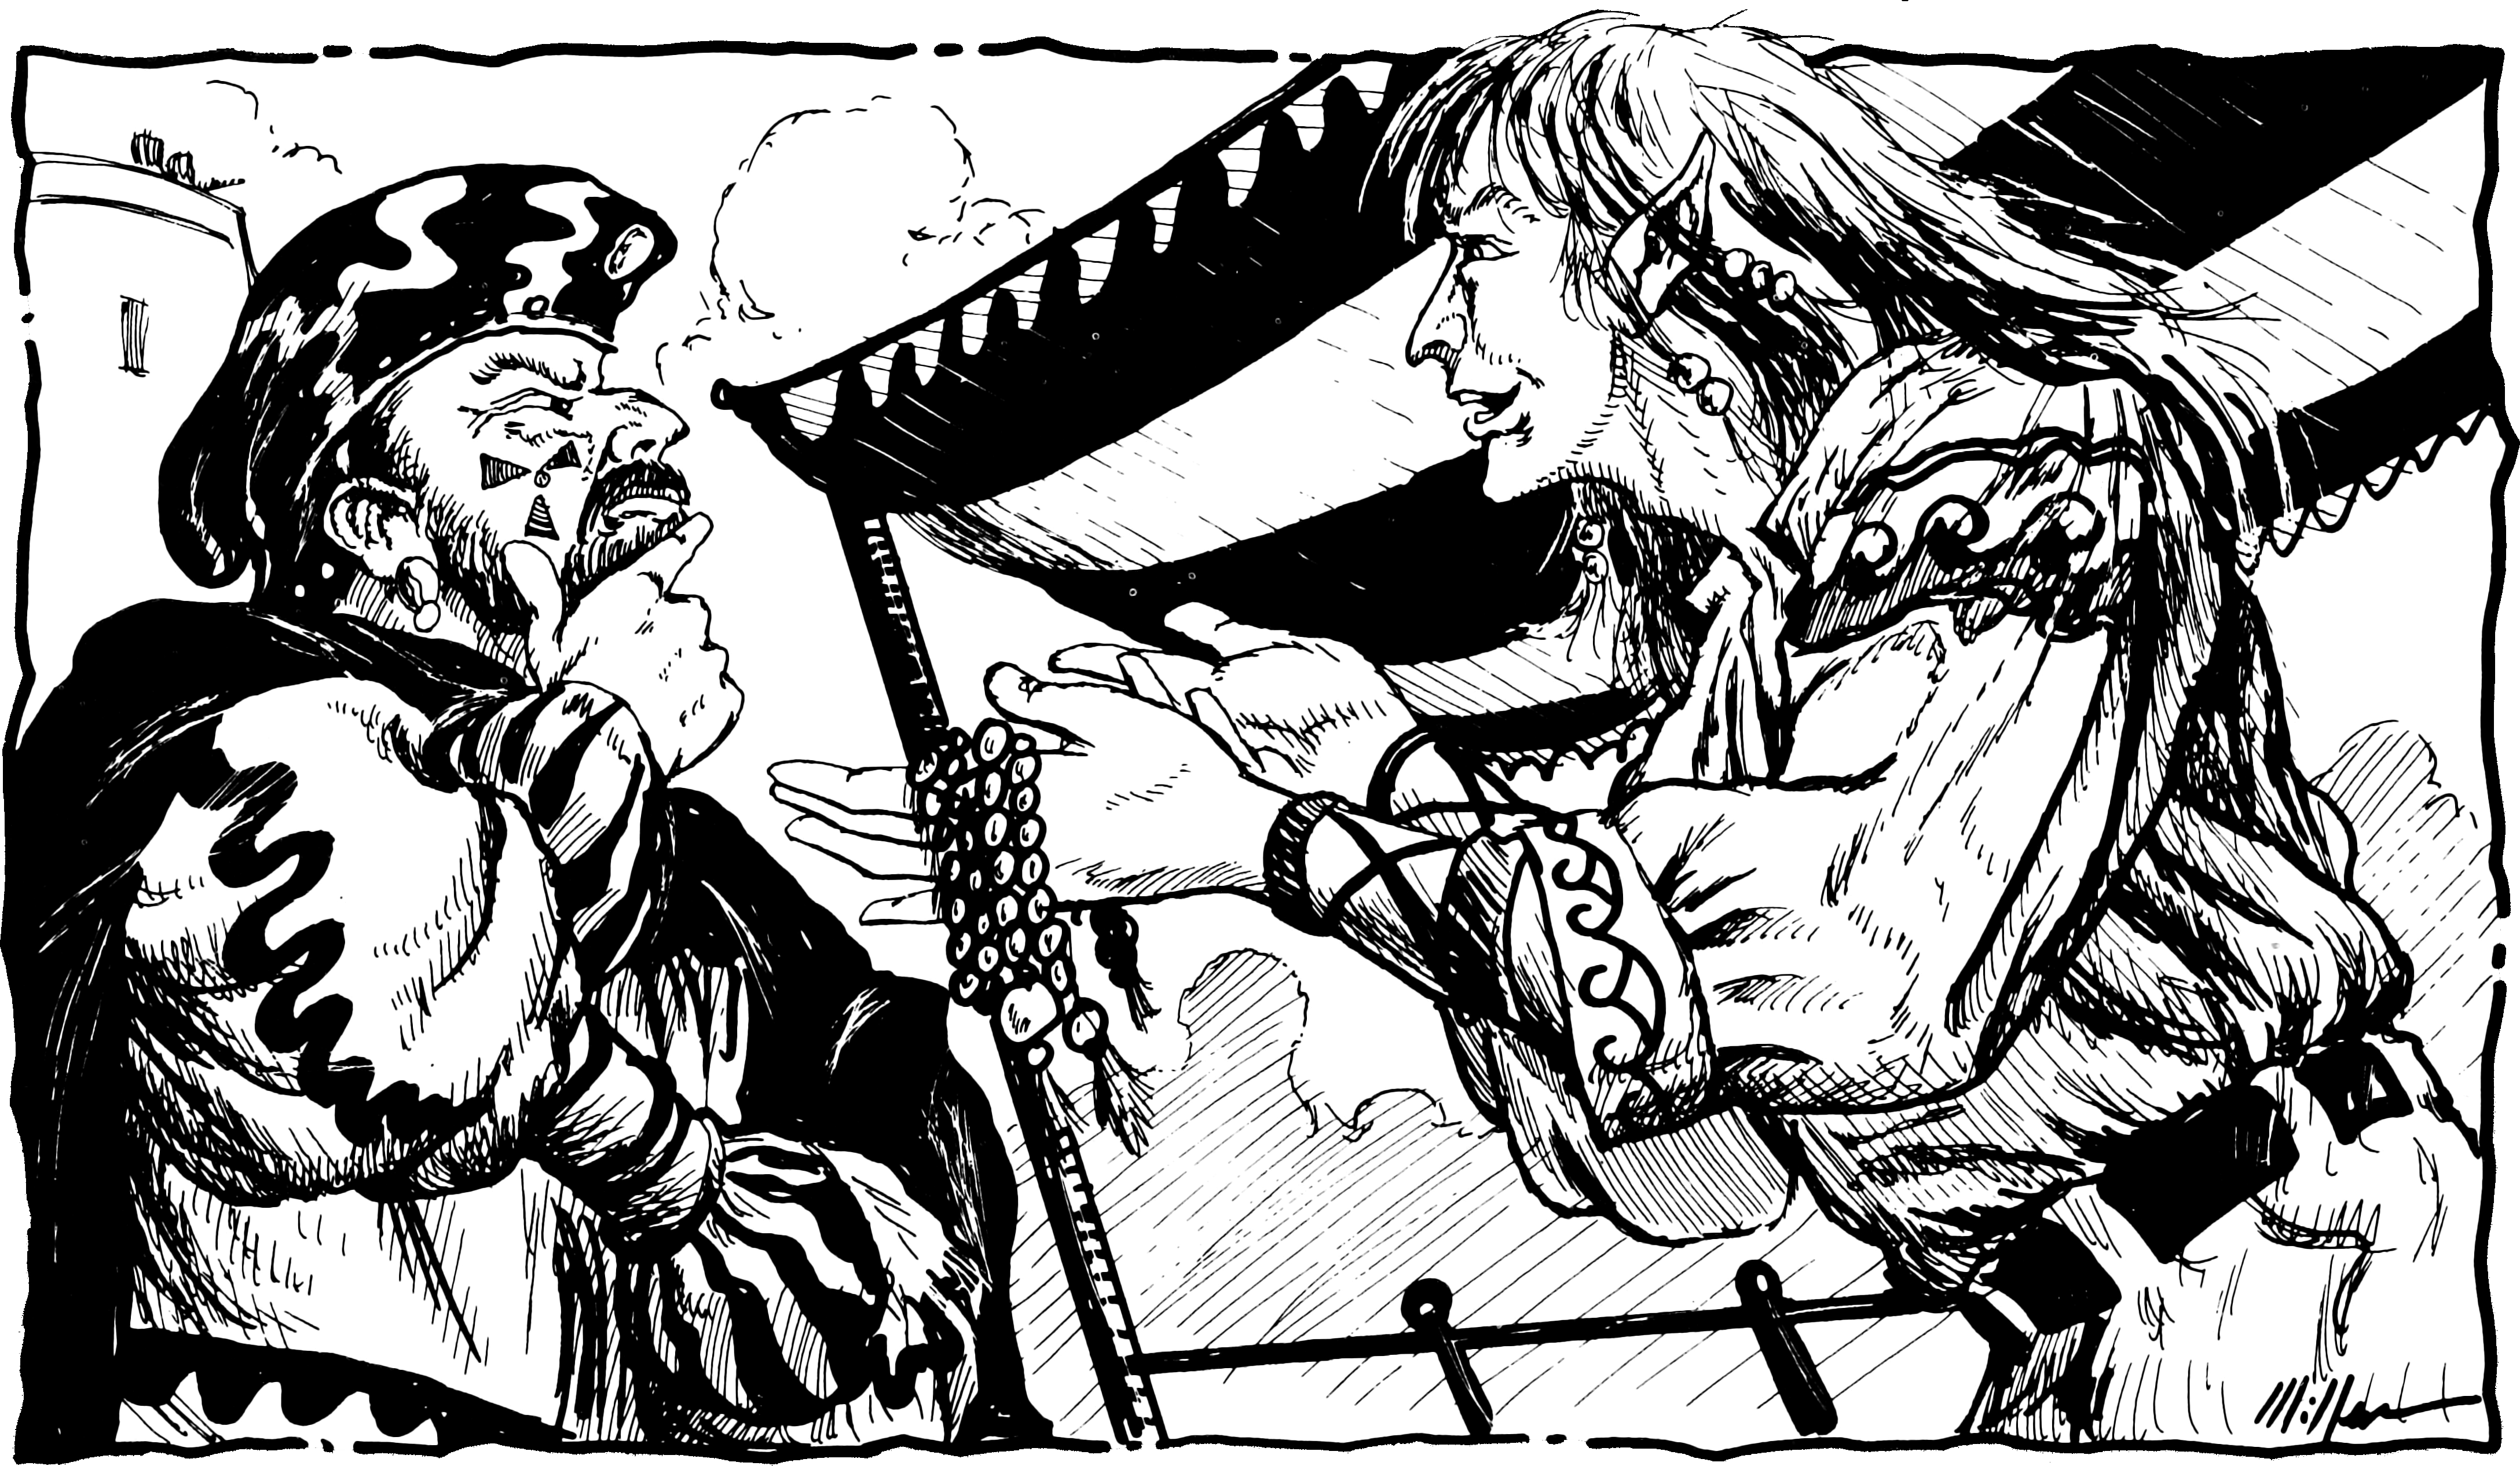
\includegraphics[width=\textwidth]{images/merchant-1.png}
\par\textit{\small\textcopyright Wizards of the Coast, 2020.}
\end{figure*}

\subsection{Adventuring Gear}

\Table{Adventuring Gear}{l RRRR}{
&& \multicolumn{3}{c}{\tableheader Weight}\\
\cmidrule[0.5pt]{3-5}
\tableheader Goods & \tableheader Cost & \tableheader M & \tableheader S & \tableheader L\\
Backpack (empty) & 2 cp & 1 kg & 0.25 kg & 4 kg\\
Barrel (empty) & 2 cp & 15 kg & &\\
Basket (empty) & 4 bits & 0.5 kg & &\\
Bedroll & 1 bits & 2.5 kg & 2.5 kg & 2.5 kg\\
Bell & 1 cp & & &\\
Blanket, winter & 5 bits & 1.5 kg & 0.37 kg & 6 kg\\
Block and tackle & 5 cp & 2.5 kg & &\\
Bottle, wine, glass & 2 cp & & &\\
Bucket (empty) & 5 bits & 1 kg & &\\
Caltrops & 1 cp & 1 kg & &\\
Candle & 1 bd & & &\\
Canvas (sq. m.) & 1 bits & 0.5 kg & &\\
Case, map or scroll & 1 cp & 0.25 kg & &\\
Chain (3 m.) & 30 cp & 1 kg & &\\
Chalk, 1 piece & 1 bd & & &\\
Chest (empty) & 2 cp & 12.5 kg & &\\
Crowbar & 2 cp & 2.5 kg & &\\
Firewood (per day) & 1 bd & 10 kg & &\\
Fishhook & 1 bits & & &\\
Fishing net, 2 sq. m. & 4 cp & 2.5 kg & &\\
Flask (empty) & 3 bd & 0.75 kg & &\\
Flint and steel & 1 cp & & &\\
Grappling hook & 1 cp & 2 kg & &\\
Hammer & 5 bits & 1 kg & &\\
Ink (30 ml vial) & 8 cp & & &\\
Inkpen & 1 bits & & &\\
Jug, clay & 3 bd & 9 lb. & &\\
Ladder, 3-meter & 5 bd & 10 kg & &\\
Lamp, common & 1 bits & 0.5 kg & &\\
Lantern, bullseye & 12 cp & 1.5 kg & &\\
Lantern, hooded & 7 cp & 1 kg & &\\
Lock (very simple) & 20 cp & 0.5 kg & &\\
Lock (average) & 40 cp & 0.5 kg & &\\
Lock (good) & 80 cp & 0.5 kg & &\\
Lock (amazing) & 150 cp & 0.5 kg & &\\
Manacles & 15 cp & 1 kg & &\\
Manacles, masterwork & 50 cp & 1 kg & &\\
Mirror, small steel & 10 cp & 0.25 kg & &\\
Mug/Tankard, clay & 2 bd & 0.5 kg & &\\
Oil (500 ml flask) & 1 bits & 0.5 kg & &\\
Paper (sheet) & 4 bits & & &\\
Parchment (sheet) & 2 bits & & &\\
Pick, miner's & 3 cp & 5 kg & &\\
Pitcher, clay & 2 bd & 2.5 kg & &\\
Piton & 1 bits & 0.25 kg & &\\
Pole, 3-meter & 2 bits & 4 kg & &\\
Pot, iron & 5 bits & 5 kg & &\\
Pouch, belt (empty) & 1 cp & 0.25 kg & 0.06 kg & 1 kg\\
Ram, portable & 10 cp & 10 kg & &\\
Rations, trail (per day) & 5 bits & 0.5 kg & 0.12 kg & 2 kg\\
Rope, giant hair (15 m.) & 50 cp & 5 kg & &\\
Rope, hempen (15 m.) & 1 cp & 5 kg & &\\
Rope, silk (15 m.) & 10 cp & 2.5 kg & &\\
Sack (empty) & 1 bits & 0.25 kg & 0.06 kg & 1 kg\\
Sealing wax & 1 cp & 0.5 kg & &\\
Sewing needle & 5 bits & & &\\
Signal whistle & 8 bits & & &\\
Signet ring & 5 cp & & &\\
Sledge & 1 cp & 5 kg & &\\
Soap (per 0.5 kg) & 5 bits & 0.5 kg & &\\
Spade or shovel & 2 cp & 4 kg & &\\
Spyglass & 1,000 cp & 0.5 kg & &\\
Tent & 10 cp & 10 kg & 2.5 kg & 40 kg\\
Torch & 1 bd & 0.5 kg & &\\
Vial, ink or potion & 1 cp & 0.05 kg & &\\
Waterskin & 1 cp & 2 kg & 0.5 kg & 8 kg\\
Whetstone & 2 bd & 0.5 kg & &\\
}


Some items weight differently for Small or Large characters, these items weigh one-quarter of the Medium-sized when made for Small characters and weigh four times as much the normal weight when made for Large characters. Containers for Small characters also carry one-quarter the normal amount, while containers for Large characters carry four times as much the normal amount.

A few of the pieces of adventuring gear are described below, along with any special benefits they confer on the user (``you'').


\textbf{Caltrops:} A caltrop is a four-pronged iron spike crafted so that one prong faces up no matter how the caltrop comes to rest. You scatter caltrops on the ground in the hope that your enemies step on them or are at least forced to slow down to avoid them. One 1-kilogram bag of caltrops covers an area 1.5 meter square.

Each time a creature moves into an area covered by caltrops (or spends a round fighting while standing in such an area), it might step on one. The caltrops make an attack roll (base attack bonus +0) against the creature. For this attack, the creature's shield, armor, and deflection bonuses do not count. If the creature is wearing shoes or other footwear, it gets a +2 armor bonus to AC. If the caltrops succeed on the attack, the creature has stepped on one. The caltrop deals 1 point of damage, and the creature's speed is reduced by one-half because its foot is wounded. This movement penalty lasts for 24 hours, or until the creature is successfully treated with a DC 15 \skill{Heal} check, or until it receives at least 1 point of magical curing. A charging or running creature must immediately stop if it steps on a caltrop. Any creature moving at half speed or slower can pick its way through a bed of caltrops with no trouble.

Caltrops may not be effective against unusual opponents.

\textbf{Candle:} A candle dimly illuminates a 1.5-meter radius and burns for 1 hour.

\textbf{Chain:} Chain has hardness 10 and 5 hit points. It can be burst with a DC 26 Strength check.

\textbf{Crowbar:} A crowbar grants a +2 circumstance bonus on Strength checks made for such purposes. If used in combat, treat a crowbar as a one-handed improvised weapon that deals bludgeoning damage equal to that of a club of its size.

\textbf{Flint and Steel:} Lighting a torch with flint and steel is a full-round action, and lighting any other fire with them takes at least that long.

\textbf{Grappling Hook:} Throwing a grappling hook successfully requires a \skill{Use Rope} check (DC 10, +2 per 3 meters of distance thrown).

\textbf{Hammer:} If a hammer is used in combat, treat it as a one-handed improvised weapon that deals bludgeoning damage equal to that of a spiked gauntlet of its size.

\textbf{Ink:} This is black ink. You can buy ink in other colors, but it costs twice as much.

\textbf{Jug, Clay:} This basic ceramic jug is fitted with a stopper and holds 4 liters of liquid.

\textbf{Lamp, Common:} A lamp clearly illuminates a 4.5-meter radius, provides shadowy illumination out to a 9-meter radius, and burns for 6 hours on 500 ml of oil. You can carry a lamp in one hand.

\textbf{Lantern, Bullseye:} A bullseye lantern provides clear illumination in a 18-meter cone and shadowy illumination in a 36-meter cone. It burns for 6 hours on 500 ml of oil. You can carry a bullseye lantern in one hand.

\textbf{Lantern, Hooded:} A hooded lantern clearly illuminates a 9-meter radius and provides shadowy illumination in a 18-meter radius. It burns for 6 hours on 500 ml of oil. You can carry a hooded lantern in one hand.

\textbf{Lock:} The DC to open a lock with the \skill{Open Lock} skill depends on the lock's quality: simple (DC 20), average (DC 25), good (DC 30), or superior (DC 40).

\textbf{Manacles and Manacles, Masterwork:} Manacles can bind a Medium creature. A manacled creature can use the \skill{Escape Artist} skill to slip free (DC 30, or DC 35 for masterwork manacles). Breaking the manacles requires a Strength check (DC 26, or DC 28 for masterwork manacles). Manacles have hardness 10 and 10 hit points.

Most manacles have locks; add the cost of the lock you want to the cost of the manacles.

For the same cost, you can buy manacles for a Small creature.

For a Large creature, manacles cost ten times the indicated amount, and for a Huge creature, one hundred times this amount. Gargantuan, Colossal, Tiny, Diminutive, and Fine creatures can be held only by specially made manacles.

\textbf{Oil:} A pint of oil burns for 6 hours in a lantern. You can use a flask of oil as a splash weapon. Use the rules for alchemist's fire, except that it takes a full round action to prepare a flask with a fuse. Once it is thrown, there is a 50\% chance of the flask igniting successfully.

You can pour a pint of oil on the ground to cover an area 1.5 meter square, provided that the surface is smooth. If lit, the oil burns for 2 rounds and deals 1d3 points of fire damage to each creature in the area.

\textbf{Ram, Portable:} This iron-shod wooden beam gives you a +2 circumstance bonus on Strength checks made to break open a door and it allows a second person to help you without having to roll, increasing your bonus by 2.

\textbf{Rope, Giant Hair:} This rope has 5 hardness, 2 hit points and can be burst with a DC 30 Strength check.

\textbf{Rope, Hempen:} This rope has 2 hit points and can be burst with a DC 23 Strength check.

\textbf{Rope, Silk:} This rope has 4 hit points and can be burst with a DC 24 Strength check. It is so supple that it provides a +2 circumstance bonus on \skill{Use Rope} checks.

\textbf{Spyglass:} Objects viewed through a spyglass are magnified to twice their size.

\textbf{Torch:} A torch burns for 1 hour, clearly illuminating a 6-meter radius and providing shadowy illumination out to a 12-meter radius. If a torch is used in combat, treat it as a one-handed improvised weapon that deals bludgeoning damage equal to that of a gauntlet of its size, plus 1 point of fire damage.

\textbf{Vial:} A vial holds 30 milliliters of liquid. The stoppered container usually is no more than 3 centimeters wide and 8 centimeters high.

\subsection{Special Substances And Items}
The following items are often, but not always available for sale in the Bard's Quarter of most city-states. Contacting someone willing to sell these and other associated goods usually requires proficient use of the \skill{Bluff}, \skill{Diplomacy}, and/or \skill{Gather Information} skills.

Any of these substances except for the everburning torch and holy water can be made by a character with the \skill{Craft} (alchemy) skill.

\ItemTable{Special Substances and Items}{
Acid (flask) & 10 cp & 0.5 kg\\
Alchemist's fire (flask) & 20 cp & 0.5 kg\\
Antitoxin (vial) & 50 cp &\\
Balican sting & 5 cp & 0.5 kg\\
Chitin ointment & 40 cp & 0.5 kg\\
Draxia ointment & 20 cp & 0.5 kg\\
Esperweed & 250 cp &\\
Everburning torch & 110 cp & 0.5 kg\\
Holy water (flask) & 25 cp & 0.5 kg\\
Hypnotic brew & 30 cp & 0.5 kg\\
Ignan tallgrass & 100 cp &\\
Kuzza powder & 20 cp &\\
Ranike sap (1 liter) & 2 cp & 0.5 kg\\
Smokestick & 20 cp & 0.25 kg\\
\TableSubheader{Splash-globe}&&\\
~ Acid & 10 cp &\\
~ Kip pheromones & 30 cp &\\
~ Liquid darkness & 10 cp &\\
~ Liquid dust & 10 cp &\\
~ Liquid fire & 10 cp &\\
~ Liquid light & 10 cp &\\
~ Poison & Poison cost $\times$ 1.5 &\\
~ Ranike sap smoke & 10 cp &\\
~ Stench cloud & 50 cp &\\
~ Stun cloud & 35 cp &\\
Sunrod & 2 cp & 0.5 kg\\
Tanglefoot bag & 50 cp & 2 kg\\
Thunderstone & 30 cp & 0.5 kg\\
Tindertwig & 1 cp &\\
}

\textbf{Acid:} You can throw a flask of acid as a splash weapon. Treat this attack as a ranged touch attack with a range increment of 3 meters. A direct hit deals 1d6 points of acid damage. Every creature within 1.5 meter of the point where the acid hits takes 1 point of acid damage from the splash.

\textbf{Alchemist's Fire:} You can throw a flask of alchemist's fire as a splash weapon. Treat this attack as a ranged touch attack with a range increment of 3 meters.

A direct hit deals 1d6 points of fire damage. Every creature within 1.5 meter of the point where the flask hits takes 1 point of fire damage from the splash. On the round following a direct hit, the target takes an additional 1d6 points of damage. If desired, the target can use a full-round action to attempt to extinguish the flames before taking this additional damage. Extinguishing the flames requires a DC 15 Reflex save. Rolling on the ground provides the target advantage on the save. Leaping into a lake or magically extinguishing the flames automatically smothers the fire.

\textbf{Antitoxin:} If you drink antitoxin, you get a +5 alchemical bonus on Fortitude saving throws against poison for 1 hour.

\textbf{Balican Sting:} This mixture of many vegetal irritants is used in conjunction with the flint-tipped javelin of the Balican fleet. Bards working for the late king Andropinis developed the substance to improve the damage done by his warriors fighting against the thick-skinned giants. This mixture, which is only effective against giants of the beasthead, crag, desert, or plains variety, causes the wound made by a balican javelin that breaks within it to itch. Unless a DC 15 Wisdom check is made by the giant on each of the following 1d4 rounds, he will scratch and inadvertently rub the shallow shards deeper, causing an additional 1d4 points of damage for each failed check.

\textbf{Chitin Ointment:} This salve is used to cure damaged chitin on kreens and other insectoid creatures. Once applied, as a standard action, this substance mends brittle or broken chitin, effectively stabilizing the creature if it had less than 0 hit points. Applying this substance to non-chitinous creatures produces no effects.

\textbf{Draxia Ointment:} The draxia weed grows on the islands of the Sea of Silt. It can be turned into an ointment that repels silt spawn by mixing the plant's juices with oil or fat. The ointment, when applied to the skin, emits a smell that repels silt spawn for two hours. Silt spawn will not come within 3 meters of a creature or object coated with draxia ointment. Although adult silt horrors find the smell irritating, they are usually unaffected by it. Sometimes silt horrors are irritated to such a level, however, that they may attack the creature or object giving off the smell. There is a 60\% chance that a silt horror will ignore all other targets and instead attack a character or object that smells of draxia weed.

\textbf{Everburning Torch:} This otherwise normal torch has a continual flame spell cast upon it. An everburning torch clearly illuminates a 6-meter radius and provides shadowy illumination out to a 12-meter radius.

\textbf{Holy Water:} Holy water damages undead creatures and evil outsiders almost as if it were acid. A flask of holy water can be thrown as a splash weapon.

Treat this attack as a ranged touch attack with a range increment of 3 meters. A flask breaks if thrown against the body of a corporeal creature, but to use it against an incorporeal creature, you must open the flask and pour the holy water out onto the target. Thus, you can douse an incorporeal creature with holy water only if you are adjacent to it. Doing so is a ranged touch attack that does not provoke attacks of opportunity.

A direct hit by a flask of holy water deals 2d4 points of damage to an undead creature or an evil outsider. Each such creature within 1.5 meter of the point where the flask hits takes 1 point of damage from the splash.

Temples to good deities sell holy water at cost (making no profit).

\textbf{Ignan Tallgrass:} A redish plant that grows in the Burning Plains near the Last Sea, ignan tallgrass can be harvested from the plains after flashfires, when they are easily spotted in small clumps untouched by the fires. Ignan tallgrass is tough and can be used to make mats and roofs of twinned fibers that stay fireproof for several months, if the harvesters are brave enough to face the flashfires to get to it, as the plant cannot be cultivated. If ignan tallgrass is sun-dried, crushed, and ingested within a week of it being picked, unless somehow magically kept fresh (as through the nurturing seeds spell), it confers resistance to fire 1 for one hour.

\textbf{Kuzza Powder:} Kuzza peppers are very hot. Typically, these vivid red peppers, when ripe, measure 2 to 2 1/2 inches long. These peppers are sometimes dried and ground into a powder by unscrupulous gladiators who use a blowpipe to blow the powder on a target, causing sever irritation. Treat this blowpipe as a blowgun with half the range increment. Filling a blowpipe is a move action that provokes attacks of opportunity. A direct hit blinds a creature for 1 round unless it makes a Fortitude save (DC 15). Every creature within 1.5 meter of the target takes a $-2$ penalty to \skill{Search} and \skill{Spot} checks for 5 rounds.

\textbf{Ranike Sap:} The sap of the ranike tree, which constantly runs down its bark, is toxic to insects. Gulg posesses the secret of safely extracting large quantities of sap from this tree, effectively milking the tree in a process called ``bleeding''. If a liter of the sap is poured in a large receptacle, such as a brazier, and lit afire, a clear smoke that impairs neither vision or breathing forms, filling a 15-meter cube (a moderate or stronger wind dissipates the smoke in 5 rounds). The smoke repels mundane insects, while giant insects, or those creatures that can be categorised as insect-like (such as antloids, kanks, and thri-kreen), that breathe or contact the smoke must make a Fortitude save (DC 15) each round for one minute; failure indicates that they are sickened for that round. The sap burns 1 hour for each liter of sap in the receptacle, after which the smoke dissipates naturally.

A shallow depression in the ground several meters wide can replace the need for a receptacle. The sap can also be used to deliniate an area---each liter poured on the ground can create a line a few inches wide and 3 meters long. When such a line is set afire, it burns for 1 minute and creates smoke in an area 3 meters long by 1.5 meter wide and high.

\textbf{Smokestick:} This alchemically treated wooden stick instantly creates thick, opaque smoke when ignited. The smoke fills a 3-meter cube (treat the effect as a fog cloud spell, except that a moderate or stronger wind dissipates the smoke in 1 round). The stick is consumed after 1 round, and the smoke dissipates naturally.

\textbf{Splash-globes:} Splash-globes are spherical glass jars containing contact poison or up to half a pint of some alchemical fluid. In addition to bursting on impact like any grenade, splash-globes can be placed in hinged pelota, thus giving the grenade additional range when fired through a splash-bow or dejada. The following types of splash-globes are available:

 \textit{Acid:} Standard flask acid can be placed in splash-globes.

 \textit{Contact Poison:} Any contact poison can be placed in a splash-globe.

 \textit{Kip Pheromones:} This splash-globe is commonly crafted by bards using kip pheromones collected by dwarven kip herders. The liquid contained within the globe is an alchemical mixture that turns into smoke on contact with air. The smoke produced is clear and does not impair vision or breathing, filling a 3-meter cube for one minute (a moderate or stronger wind dissipates the smoke in 1 round). Those within the smoke must make a DC 15 Fortitude save each round they are in contact with it or become fascinated for the as long as the smoke remains. Dwarves gain a +4 racial bonus on their Fortitude save against kip pheromones.

 \textit{Liquid Darkness:} Anyone struck directly by liquid darkness must make a Reflex save (DC 15) or be blinded for one minute. Those splashed with liquid darkness have their vision blurred for one minute if they fail a DC 15 Reflex save, granting their opponents concealment. In addition, all natural fires within the splash area are instantly extinguished. Liquid darkness immediately extinguishes liquid light.

 \textit{Liquid Dust:} The liquid from this splash-globe turns into dust on contact with the air. You can use this liquid to cover up to 20 1.5-meter squares of tracks. On impact, liquid dust forms a 4.5-meter diameter cloud, three meters high that lasts one round. Alternately, liquid dust can be launched via slash-globes. Anyone struck directly by liquid dust must make a DC 15 Fortitude save each round for one minute; failure dictates that they are nauseated for that round. Those splashed with liquid dust suffer the same effect for one round if they fail a DC 15 Fortitude save.

 \textit{Liquid Fire:} Alchemist's fire can be placed in splash-globes.

 \textit{Liquid Light:} This splash-globe contains two liquids that mix together when the splash-globe is ruptured. The resulting mixture glows for eight hours. If you break the liquid light globe while it is still in its pouch, the pouch can serve as a light source just like a sunrod. Anyone struck directly by liquid light must make a DC 20 Fortitude save or be temporarily dazzled ($-1$ on all attack rolls) for 1 minute, and will glow in darkness for eight hours unless they somehow cover the affected areas. Creatures splashed with liquid light (see grenade rules) also glow in the darkness, but are not blinded.

 \textit{Ranike Sap Smoke:} The liquid from this splash-globe is an alchemical mixture of ranike sap that turns into smoke on contact with air. The smoke produced is clear and does not impair vision or breathing, filling a 3-meter cube (a moderate or stronger wind dissipates the smoke at the end of the character's action). The smoke repels mundane insects, while giant insects, or those creatures that can be categorised as insect-like (such as antloids, kanks, and thri-kreens), that breath or enter in contact with the smoke must make a DC 15 Fortitude save each round for one minute; failure indicates that they are sickened for that round. This small quantity of sap only reacts with the air for 1 round, after which the smoke dissipates naturally.

 \textit{Stench Cloud:} The liquid inside this splash-globe is crafted from fordorran musk and stinkweed extract. The foul liquid turns into smoke on contact with air. The smoke produced is clear and does not impair vision or breathing, filling a 3-meter cube for one minute (a moderate or stronger wind dissipates the smoke in 1 round). Those within the smoke must make a DC 15 Fortitude save each round they are in contact with it or become nauseated for as long as they remain in contact with the cloud.

 \textit{Stun Cloud:} The liquid inside this splash-globe is crafted from boiled floater jelly combined with the pulped spines from a poisonous cactus. The liquid turns into smoke on contact with air. The smoke produced is clear and does not impair vision or breathing, filling a 3-meter cube for one minute (a moderate or stronger wind dissipates the smoke in 1 round). Those within the smoke must make a DC 15 Fortitude save each round they are in contact with it or become stunned for as long as they remain in contact with the cloud.

\textbf{Sunrod:} This 30-centimeter long, gold-tipped, iron rod glows brightly when struck. It clearly illuminates a 9-meter radius and provides shadowy illumination in a 18-meter radius. It glows for 6 hours, after which the gold tip is burned out and worthless.

\textbf{Tanglefoot Bag:} When you throw a tanglefoot bag at a creature (as a ranged touch attack with a range increment of 3 meters), the bag comes apart and the goo bursts out, entangling the target and then becoming tough and resilient upon exposure to air. An entangled creature takes a $-2$ penalty on attack rolls and a $-4$ penalty to Dexterity and must make a DC 15 Reflex save or be glued to the floor, unable to move. Even on a successful save, it can move only at half speed. Huge or larger creatures are unaffected by a tanglefoot bag. A flying creature is not stuck to the floor, but it must make a Reflex save (DC 15) or be unable to fly (assuming it uses its wings to fly) and fall to the ground. A tanglefoot bag does not function underwater.

A creature that is glued to the floor (or unable to fly) can break free by making a DC 17 Strength check or by dealing 15 points of damage to the goo with a slashing weapon. A creature trying to scrape goo off itself, or another creature assisting, does not need to make an attack roll; hitting the goo is automatic, after which the creature that hit makes a damage roll to see how much of the goo was scraped off. Once free, the creature can move (including flying) at half speed. A character capable of spellcasting who is bound by the goo must make a \skill{Concentration} check (DC 15) to cast a spell. The goo becomes brittle and fragile after 2d4 rounds, cracking apart and losing its effectiveness. An application of universal solvent to a stuck creature dissolves the alchemical goo immediately.

\textbf{Thunderstone:} You can throw this stone as a ranged attack with a range increment of 6 meters. When it strikes a hard surface (or is struck hard), it creates a deafening bang that is treated as a sonic attack. Each creature within a 3-meter-radius spread must make a DC 15 Fortitude save or be deafened for 1 hour. A deafened creature, in addition to the obvious effects, takes a $-4$ penalty on initiative and has a 20\% chance to miscast and lose any spell with a verbal component that it tries to cast.

Since you don't need to hit a specific target, you can simply aim at a particular 1.5-meter square. Treat the target square as AC 5.

\textbf{Tindertwig:} The alchemical substance on the end of this small, wooden stick ignites when struck against a rough surface. Creating a flame with a tindertwig is much faster than creating a flame with flint and steel (or a magnifying glass) and tinder. Lighting a torch with a tindertwig is a standard action (rather than a full-round action), and lighting any other fire with one is at least a standard action.
\subsectionA{Metaempiric Components}
Useful for spellcasters, these items are special material components that have a chance of influencing the casting of certain spells while held in hand. Since a metempiric component must be held in one hand to use, it cannot be used in conjunction with the \feat{Still Spell} feat and, being optional for the casting of a spell, does not count as a normal material component for the purpose of the \feat{Eschew Materials} feat. Metempiric components are consumed during the casting of a spell, unless otherwise noted.

\ItemTable{Metaempiric Components}{
Aviarag horn & 1,350 cp & 2.5 kg\\
Beasthead blood & 45 cp & 0.5 kg\\
Dagorran crystal, diminutive & 100 cp &\\
Dagorran crystal, tiny & 300 cp & 0.25 kg\\
Defiler's ash & 1,700 cp &\\
Defiled poisonweed petals & 350 cp &\\
Eagle beasthead feather & 40 cp &\\
Roc feather & 450 cp &\\
Royal justice token & 1,375 cp & 0.5 kg\\
Shadow giant fumes & 390 cp & 0.5 kg\\
Sun paraelemental essence & 935 cp & 0.5 kg\\
T'chowb's thalamus & 1,250 cp & 0.25 kg\\
}

\textbf{Aviarag Horn:} A horn willingly given by an aviarag for use by someone after its passing into death is a powerful weapon for those seeking to do good. When presented while casting a spell, the goodness still emanating from the beast's horn is so tangible that the spell itself benefits from it. When used as a component for any spell with the good descriptor, the aviarag horn increases the spell's effective caster level by 1d4. An aviarag horn is not consumed after being used.

\textbf{Beasthead Blood:} As sorcerous mutations of normal Athasian giants, the blood of beasthead giants has some magical properties. When beasthead blood is used as a component in any transmutation spell, it increases the spell's saving throw DC by +1. Inexplicably, only druids and preservers may use beasthead blood this way; it provides no benefit for other types of spellcasters.

\textbf{Dagorran Crystal:} This green crystal growth is extracted from the body of a daggoran. Daggorans come in two sizes, which affect the size and potency of the crystal: a Medium daggoran provides a Diminutive crystal while a Large daggoran provides a Tiny crystal. When used as a component for a spell with the mind-affecting descriptor, a Diminutive daggoran crystal increases the spell's saving throw DC by +2.

\textbf{Defiler's Ash:} Mixed in with a special mixture of blood, these ashes must be taken from at least three different spellcasters' ashen circles caused by powerful spellcasting (spell level 6th and above). When used in the casting of a spell with the necromancy descriptor, defiler's ash empower the spell as if the caster had applied the Empower Spell feat (but without changing the spell's effective level or increasing its casting time).

\textbf{Defiled Poisonweed Petals:} The bright orange petals of a poisonweed plant turned undead by the action of defiling represent the epitome of noxiousness. When used as a component for any spell with the death descriptor, the petals of a defiled poisonweed increase the spell's saving throw DC by +2.

\textbf{Eagle Beasthead Feather:} If a feather from an eagle-headed beasthead giant is in hand when falling, it can be used as a component when casting feather fall, doubling the duration of the spell.

\textbf{Roc Feather:} These huge feathers---from anywhere between 0.6 and 1.2 meter long---come from an Athasian rock. When used as a component for a spell confering flight, a roc feather doubles the spell's duration.

\textbf{Royal Justice Token:} Only used by templars in the service of the sorcerer-monarch for which the token was created, the royal justice token shows graven symbols associated with the justice system used in a particular city-state. Symbols include ever-vigilant eyes, readied swords, and open hand or closed fist. When used as a component for the \spell{wrath of the sorcerer-king} spell, the token increases the spell's effective caster level by +2. A royal justice token is not consumed after being used.

\textbf{Shadow Giant Fumes:} If bottled, the black, cold fumes that emanate from a shadow giant's mouth as it speaks can be used to enhance spells that have a connection to the Black. When used as a component for the spells \spell{greater shadow conjuration}, \spell{shades}, or \spell{shadow conjuration}, the potency of the spell is one-fifth (20\%) better than normal.

\textbf{Sun Paraelemental Essence:} This bright and blinding essence comes from a dead sun paraelemental of at least Huge size. The essence must be trapped in a clear crystal container within one minute of the elemental's death and must always be kept under the light of the sun during the day, or else losing its potency. During the night, the light fades and gives off the same illumination as a candle. When used as a component for any spell with the light descriptor, the essence increases the effective caster level by +2.

\textbf{T'chowb's Thalamus:} The thalamus of a recently fed (within the last 24 hours) t'chowb is said to be seething with absorbed intelligence. When used as a metempiric component, the t'chowb's thalamus gives the caster a +10 circumstance bonus on caster level checks made to overcome a target's spell resistance.
\subsection{Psychoactive Components}
Useful for manifesters, these items are components that have a chance of influencing the manifestation of certain powers when used properly. Unlike metempiric components, each psychoactive component must be used in a specific fashion in order to provide its benefits to the manifester. Unless otherwise noted, psychoactive components are consumed during the manifesting of a power.

Also included in this category is a creature sometimes used by psionic characters to access the residual psionic energy their mind's produce throughout the day.

\ItemTable{Psychoactive Components}{
Aviarag horn melange & 250 cp & 0.5 kg\\
Bouyan crystal & 400 cp & 1 kg\\
Cilops compound eye & 65 cp & \\
Dagorran crystal, diminutive & 100 cp & \\
Dagorran crystal, tiny & 300 cp & \onequarter kg\\
Tas'l worm & 100 cp & \\
T'chowb's thalamus & 1,250 cp & \onequarter kg\\
}

\textbf{Aviarag Horn Melange:} The great horn of the noble aviarag, when crushed and mixed with a specially treated wine, preserves some of the psionic power of the aviarag and can expand the reach and power of the drinker's mind. A manifester drinking this psychoactive substance no more than 1 minute before using the \psionic{mindwipe} power increases the power's save DC by +2, and drinking it before manifesting \psionic{mindlink} doubles the power's range, as per the \feat{Enlarge Power} feat (but without changing the power's effective level or requiring the expendature of a psionic focus). Drinking this melange is a standard action that provokes attacks of opportunity.

\textbf{Bouyan Crystal:} From salt formations found within the great salt plains, the clear gray bouyan stone is cut to a great degree of perfection, allowing a manifester to focus his mind upon it. A manifester that concentrates upon a held bouyan crystal when manifesting any telepathy power (a free action, assuming the manifester is already holding the component) increases the power's effective manifester level by +1.

\textbf{Cilops Compound Eye:} Crushing the central compound eye of a cilops produces a thick jelly that may extend the user's senses of his surroundings. If this jelly is spread over the eyes of a character (a full-round action) before he manifests object reading, and the temporary blindness it induces is endured for the extent of the power's duration, then this power always successfully identifies all other former owners of an object in sequence, with no chance that former owners will be skipped and thus not identified. Removing the jelly from one's eyes, thus negating the blindness, takes 1 minute. Eating the jelly before manifesting sensitivity to psychic impressions reduces the manifesting time of that power to 10 minutes.

\textbf{Dagorran Crystal:} This green crystal growth is extracted from the body of a daggoran. Manifesters use these crystals to harness the dagorran's ability to sense the psionic nature of creatures. A Diminutive daggoran crystal gives manifesters advantage to \skill{Psicraft} checks made when using the \psionic{psychic tracking} psionic power, while a Tiny daggoran crystal gives a +5 competence bonus. Such a crystal is not consumed when used.

\textbf{Tas'l Worm:} Tas'l worms are worms of Diminutive size, similar in appearance to ock'n, but without eyestalks. Only found on living psionic creatures, these 1-inch long worms snake slowly between the skin and the skull of their host, accumulating and living off of residual psionic energy.

A tas'l worm can be removed by cutting open the skin. A character can remove a worm by taking 10 minutes to locate and extract it from the host's scalp. The extraction does 1d6 points of damage to the victim, and has a 75\% chance of killing the worm in the process. If a successful \skill{Heal} check (DC 20) is made, the cutting damage is reduced to 1d2, with no chance of killing the worm.

A worm outside of its host lives for 1 hour. The worm, when put against the skin of a psionic creature, burrows into its flesh, causing 1 point of damage. Afterwards, the worm must stay within the host for at least 24 hours before it amasses enough residual energy to be used. Tas'l worms use the innocuous vermin statistics (see page 191 of Terrors of Athas). A worm linked to a host has a lifespan of 2d6 months. If more than one worm live on the same scalp, there is a 55\% chance for 1d2 worms to spawn each month thereafter.

The creature hosting tas'l worms can make a \skill{Concentration} check (DC 20) as a free action, once per day, to tap the energy they contain. If the check is successful, each tas'l worm hosted by a creature provides 1 power point. All worms must be tapped at once, or none at all. These power points are considered a part of the creature's own power point reserve for the purpose of using stored power points. A failed check can be retried on the character's next turn.

The hosting creature receives a cumulative $-1$ circumstance penalty to Will saves against telepathic powers for each worm living within its body, as the worms make their host more responsive to outside psionic influence.

A tas'l worm registers as psionic to \psionic{detect psionics}.

\textbf{T'chowb's Thalamus:} The thalamus of a recently fed (within the last 24 hours) t'chowb is said to be seething with absorbed intelligence. If crushed in one's hand during the manifestation of a power (a free action, assuming the manifester is already holding the component), the t'chowb's thalamus gives a manifester a +10 circumstance bonus on manifester level checks made to overcome a target's power resistance.
\subsectionA{Tools and Skill Kits}

\ItemTable{Tools and Skill Kits}{
Alchemist's lab & 500 cp & 20 kg\\
Artisan's tools & 5 cp & 2.5 kg\\
Artisan's tools, masterwork & 55 cp & 2.5 kg\\
Book of poisons & 125 cp & 1 kg\\
Candle of rejuvenation & 50 cp & \\
Climber's kit & 80 cp & 2.5 kg1\\
Concealing weave & 5 cp & 1 kg\\
Disguise kit & 50 cp & 4 kg1\\
Healer's kit & 50 cp & 0.5 kg\\
Holly and mistletoe & & \\
Holy symbol, silver & 25 cp & 0.5 kg\\
Holy symbol, wooden & 1 cp & \\
Hourglass & 25 cp & 0.5 kg\\
Magnifying glass & 100 cp & \\
Meditative kit & 35 cp & 1.5 kg\\
Musical instrument, common & 5 cp & 1.5 kg1\\
Musical instrument, masterwork & 100 cp & 1.5 kg1\\
Navigator kit & 75 cp & 5 kg\\
Remote viewing kit & & 5 kg\\
Scale, merchant's & 2 cp & 0.5 kg\\
Spell component pouch & 5 cp & 1 kg\\
Spellbook, wizard's (blank) & 15 cp & 1.5 kg\\
Thieves' tools & 30 cp & 0.5 kg\\
Thieves' tools, masterwork & 100 cp & 1 kg\\
Tool, masterwork & 50 cp & 0.5 kg\\
Water clock & 1,000 cp & 100 kg\\
}

The items described below are particularly useful to characters that have certain specific skills or abilities and are used in specific situations.


\textbf{Alchemist's Lab:} An alchemist's lab always has the perfect tool for making alchemical items, so it provides +2 circumstance bonus on \skill{Craft} (alchemy) checks. It has no bearing on the costs related to the \skill{Craft} (alchemy) skill. Without this lab, a character with the \skill{Craft} (alchemy) skill is assumed to have enough tools to use the skill but not enough to get the +2 bonus that the lab provides.

\textbf{Artisan's Tools, Masterwork:} These tools serve the same purpose as artisan's tools (above), but masterwork artisan's tools are the perfect tools for the job, so you get +2 circumstance bonus on \skill{Craft} checks made with them.

\textbf{Artisan's Tools:} These special tools include the items needed to pursue any craft. Without them, you have to use improvised tools (-2 penalty on \skill{Craft} checks), if you can do the job at all.

\textbf{Book of Poisons:} The original Book of Poisons is rumored to have been written by the half-elven bard Cabal, with current copies containing but fragments of the original poison recipes. This set of clay tablets is covered with markings, known mostly to bards, that can only be understood by making a \skill{Decipher Script} check (DC 15). Once deciphered, the reader can see that they contain a number of recipes that describe, step-by-step, tried-and-true methods for crafting specific poisons. The tablets grant the following benefits when used in conjunction with the crafting of poisons described in the set (normally 5 to 10 different poisons, of the DM's choice): +2 circumstance bonus to \skill{Craft} (poisonmaking) checks and a +1 to the save DC of the poisons being crafted. This last bonus stacks with the scorpion's touch bardic ability.

\textbf{Candle of Rejuvenation:} This item allows a manifester to recover power points as if he were resting at night. The manifester recovers 10 power points at the end of each complete hour spent within 3 meters of a lit candle. By making an \skill{Autohypnosis} DC 15 check, this amount increases by one-half. Each candle burns for a total of eight hours.

\textbf{Climber's Kit:} This is the perfect tool for climbing and gives you +2 circumstance bonus on \skill{Climb} checks.

\textbf{Concealing Weave:} This kit is composed of one or more related articles of clothing specifically made to camouflage a caster's arm and hand movements while casting a spell. This kit grants +2 circumstance bonus on \skill{Bluff} checks made to conceal the casting of spells with a somatic component.

\textbf{Disguise Kit:} The kit is the perfect tool for disguise and provides +2 circumstance bonus on \skill{Disguise} checks. A disguise kit is exhausted after ten uses.

\textbf{Healer's Kit:} It is the perfect tool for healing and provides +2 circumstance bonus on \skill{Heal} checks. A healer's kit is exhausted after ten uses.

\textbf{Holy Symbol, Silver or Wooden:} A holy symbol focuses positive energy. A cleric uses it as the focus for his spells and as a tool for turning undead. Each religion has its own holy symbol.

 \textit{Unholy Symbols:} An unholy symbol is like a holy symbol except that it focuses negative energy and is used by evil clerics (or by neutral clerics who want to cast evil spells or command undead).

 \textit{Sorcerer-king's Sigil:} A sorcerer-king's sigil is like a holy symbol for templars. It is the sign of their rank and station within the templarate. It is unique to each city-state.

\textbf{Magnifying Glass:} This simple lens allows a closer look at small objects. It is also useful as a substitute for flint and steel when starting fires. Lighting a fire with a magnifying glass requires light as bright as sunlight to focus, tinder to ignite, and at least a full-round action. A magnifying glass grants +2 circumstance bonus on \skill{Appraise} checks involving any item that is small or highly detailed.

\textbf{Meditative Kit:} This small and delicately carved crystal container produces an hypnotic rainbow-like effect while filled with clear water and struck by light. After 1 minute of uninterrupted observation of the rainbow pattern, the kit provides +2 circumstance bonus to the next \skill{Autohypnosis} check made by the viewer within the next 10 minutes.

\textbf{Musical Instrument, Common or Masterwork:} A masterwork instrument grants +2 circumstance bonus on \skill{Perform} checks involving its use.

\textbf{Navigator's Kit:} Prized posessions of many trading houses and frequent wanderers of the wastes, each of these kits is composed of a set of maps made of straight sticks representing roads, and small stones for villages, cities and others special locations, all lashed together by strings. If you succeed at a \skill{Knowledge} (geography) check DC 10 while using this kit, you gain a +4 bonus on \skill{Survival} checks made to keep from getting lost.

\textbf{Remote Viewing Kit:} This kit allows for a more potent use of the \psionic{remote viewing} power. Unlike other class or skill kits, this kit is created from local natural materials, effectively making it free in cost, but its user must recreate the kit before each use. Five ranks in \skill{Knowledge} (psionics), and 10 minutes, are required to create the kit. It must be created in silence, without distractions, and in a windless area. The kit takes the form of a 1.5-meter square patch of flat ground, covered with sand or particulate dirt to a depth of at least 2.5 centimeters, with 1d6 palm-sized stones deposited on it. Lines and circles are then traced around the stones and over the entire surface, creating a unique, maze-like pattern.

To gain the benefits of the kit, the user must focus on the patch of ground and succeed at a DC 15 \skill{Concentration} check after its creation; failure indicating that the user needs to recreate the kit anew. A successful check means the user's next manifestation of remove viewing, which must be within 1 minute of making the check, is altered in the following ways. First, the subject of the user's viewing attempt receives a $-2$ penalty to his Will saving throw against the \psionic{remote viewing}. Second, the user receives +2 circumstance bonus to \skill{Concentration} checks made to manifest a power through \psionic{remote viewing}. Finally, the user receives +2 circumstance bonus to \skill{Hide} checks to prevent his quasi-real viewpoint from being noticed by the subject he his viewing.

The effects of this kit can be made more potent if more than one character assists with its creation. Each character that helps adds another 1.5-meter square to the space taken by the kit, and another 10 minutes to the time required for the kit's completion. Each character that succeeds at a DC 15 \skill{Concentration} check at the time of the kit's completion can use the aid another action to help the user with skill checks made while the user is manifesting \psionic{remote viewing}. A kit created in this fashion is more complex, and as such requires two more ranks in \skill{Knowledge} (psionics) to create for each additional character that helped in its creation. Only a limited number of characters can help to create a remove viewing kit, equal to half the user's manifester level.

\textbf{Scale, Merchant's:} A scale grants +2 circumstance bonus on \skill{Appraise} checks involving items that are valued by weight, including anything made of precious metals.

\textbf{Spell Component Pouch:} A spellcaster with a spell component pouch is assumed to have all the material components and focuses needed for spellcasting, except for those components that have a specific cost, divine focuses, and focuses that wouldn't fit in a pouch.

\textbf{Spellbook, Wizard's (Blank):} A spellbook has 100 pages of parchment, and each spell takes up one page per spell level (one page each for 0-level spells).

\textbf{Thieves' Tools, Masterwork:} This kit contains extra tools and tools of better make, which grant +2 circumstance bonus on \skill{Disable Device} and \skill{Open Lock} checks.

\textbf{Thieves' Tools:} This kit contains the tools you need to use the \skill{Disable Device} and \skill{Open Lock} skills. Without these tools, you must improvise tools, and you have disadvantage on \skill{Disable Device} and \skill{Open Lock} checks.

\textbf{Tool, Masterwork:} This well-made item is the perfect tool for the job. It grants +2 circumstance bonus on a related skill check (if any). Bonuses provided by multiple masterwork items used toward the same skill check do not stack.

\textbf{Water Clock:} This large, bulky contrivance gives the time accurate to within half an hour per day since it was last set. It requires a source of water, and it must be kept still because it marks time by the regulated flow of droplets of water.
\subsection{Clothing}
Clothes weigh one-quarter the normal amount when made for Small characters, and four times as much when made for Large characters.

\Table{Clothing}{lRRRR}{
&& \multicolumn{3}{c}{\tableheader Weight}\\
\cmidrule[0.25pt]{3-5}
\tableheader Item & \tableheader Cost & \tableheader S & \tableheader M & \tableheader L\\
Artisan's outfit & 1 cp & 0.5 kg & 2 kg & 8 kg\\
Cleric's vestments & 5 cp & 0.75 kg & 3 kg & 12 kg\\
% Cold weather outfit & 8 cp & 3.5 kg & 3.5 kg & 15 kg\\
Courtier's outfit & 30 cp & 0.75 kg & 3 kg & 12 kg\\
Elven outfit & 30 cp & 0.62 kg & 2.5 kg & 10 kg\\
Entertainer's outfit & 3 cp & 0.5 kg & 2 kg & 8 kg\\
Explorer's outfit & 10 cp & 1 kg & 4 kg & 16 kg\\
High templar's outfit & 100 cp & 0.62 kg & 2.5 kg & 10 kg\\
% Monk's outfit & 5 cp & 1 kg & 1 kg & 1 kg\\
Noble's outfit & 75 cp & 1.25 kg & 5 kg & 20 kg\\
Peasant's outfit & 1 sp & 0.25 kg & 1 kg & 4 kg\\
Royal defiler's outfit & 80 cp & 0.62 kg & 2.5 kg & 10 kg\\
Royal outfit & 200 cp & 1.87 kg & 7.5 kg & 30 kg\\
Scholar's outfit & 5 cp & 0.75 kg & 3 kg & 12 kg\\
Slave's outfit & 2 bd & 0.12 kg & 0.5 kg & 2 kg\\
Traveler's outfit & 1 cp & 0.62 kg & 2.5 kg & 10 kg\\
Wastelander outfit & 20 cp & 0.75 kg & 3 kg & 12 kg\\
}


\textbf{Artisan's Outfit:} This outfit includes a shirt with buttons, a skirt or pants with a drawstring, shoes, and perhaps a cap or hat. It may also include a belt or a leather or cloth apron for carrying tools.

\textbf{Cleric's Vestments:} These ecclesiastical clothes are for performing priestly functions, not for adventuring.

% \textbf{Cold Weather Outfit:} A cold weather outfit includes a wool coat, linen shirt, wool cap, heavy cloak, thick pants or skirt, and boots. This outfit grants a +5 circumstance bonus on Fortitude saving throws against exposure to cold weather.

\textbf{Courtier's Outfit:} This outfit includes fancy, tailored clothes in whatever fashion happens to be the current style in the courts of the nobles. Anyone trying to influence nobles or courtiers while wearing street dress will have a hard time of it (-2 penalty on Charisma-based skill checks to influence such individuals). If you wear this outfit without jewelry (costing an additional 50 cp), you look like an out-of-place commoner.

\textbf{Elven Outfit:} Although varying greatly from tribe to tribe, all elven clothing is based around two concepts: functionality and flattery. This set of clothes most often includes a hooded cloak or stylized robes, although some outfits make do with tight leather wrappings or other heat-shielding and water-retaining materials. In regards to its other aspect---visual appeal---every elven outfit is, no matter how functional, also designed to complement the wearer's form. Each outfit is tailor-made by elves, following a particular tribal pattern, and are normally not for sale. In addition, various portions of this outfit---such as a cloak, thick shoulder scarf, or even an entire tunic---are colored, patterned, or designed to be reversible in such a way as to blend in with the Athasian landscape, helping the wearer to blend in with the terrain in sandy areas: this provides a +3 circumstance bonus on \skill{Hide} checks while in desert terrain. For twice the listed price, this outfit can be made to fit over light armor.

\textbf{Entertainer's Outfit:} This set of flashy, perhaps even gaudy, clothes is for entertaining. While the outfit looks whimsical, its practical design lets you tumble, dance, walk a tightrope, or just run (if the audience turns ugly).

\textbf{Explorer's Outfit:} This is a full set of clothes for someone who never knows what to expect. It includes sturdy boots, leather breeches or a skirt, a belt, a shirt (perhaps with a vest or jacket), gloves, and a cloak. Rather than a leather skirt, a leather overtunic may be worn over a cloth skirt. The clothes have plenty of pockets (especially the cloak). The outfit also includes any extra items you might need, such as a scarf or a wide-brimmed hat.

\textbf{High Templar's Outfit:} High templar's outfits differ for each of the Tablelands' cities. This set of clothing is made of the best material produced by a city-state's artisans and exemplifies that city's templarate. Wearing the proper high templar outfit for a city's templarate gives a +2 circumstance bonus to \skill{Diplomacy} checks in contests of the \feat{Secular Authority} feat made within that city.

% \textbf{Monk's Outfit:} This simple outfit includes sandals, loose breeches, and a loose shirt, and is all bound together with sashes. The outfit is designed to give you maximum mobility, and it's made of high-quality fabric. You can hide small weapons in pockets hidden in the folds, and the sashes are strong enough to serve as short ropes.

\textbf{Noble's Outfit:} This set of clothes is designed specifically to be expensive and to show it. Precious metals and gems are worked into the clothing. To fit into the noble crowd, every would-be noble also needs a signet ring (see Adventuring Gear, above) and jewelry (worth at least 100 cp).

\textbf{Peasant's Outfit:} This set of clothes consists of a loose shirt and baggy breeches, or a loose shirt and skirt or overdress. Cloth wrappings are used for shoes.

\textbf{Royal Defiler's Outfit:} Royal defilers, who practice sorcery with the full legal backing of a sorcerer-king, must clearly indicate their protected status if they are to be spared the mob's wrath. This set of clothing is made from the best materials available to a city-state's artisans, and is second in quality only to a templar's outfit. The outfit varies greatly from city to city. In Raam, for example, this outfit is a checkered silk robe adorned with a silver brooch denoting royal defiler status. Wearing the proper defiler outfit for a city gives a +2 circumstance bonus to \skill{Intimidate} checks against citizens who aren't part of the templarate.

\textbf{Royal Outfit:} This is just the clothing, not the royal scepter, crown, ring, and other accoutrements. Royal clothes are ostentatious, with gems, gold, silk, and fur in abundance.

\textbf{Scholar's Outfit:} Perfect for a scholar, this outfit includes a robe, a belt, a cap, soft shoes, and possibly a cloak.

\textbf{Slave's Outfit:} This simple set of clothes consists of a loincloth, or a short skirt and sleeveless tunic, all made of rough-hewn materials.

\textbf{Traveler's Outfit:} This set of clothes consists of boots, a wool skirt or breeches, a sturdy belt, a shirt (perhaps with a vest or jacket), and an ample cloak with a hood.

\textbf{Wastelander's Outfit:} Similar to clothing worn by the many elven tribes dotting the Athasian landscape, this set of clothes commonly includes a large hooded cloak, multiple layers of heat-resistant, porous cloth, and reinforced leather padding designed to protect against blowing sand, sharp rocks and the ever-present cacti needles. In addition, this outfit is colored to blend in with whatever environment the wastelander has chosen as his home, helping the wearer to blend in with rocky surroundings. This provides a +2 circumstance bonus on \skill{Hide} checks while in the appropriate terrain; each wastelander's outfit provides this bonus for a single terrain type only. For twice the price, this outfit can be made to fit over light armor.
\begin{figure*}[b!]
\centering
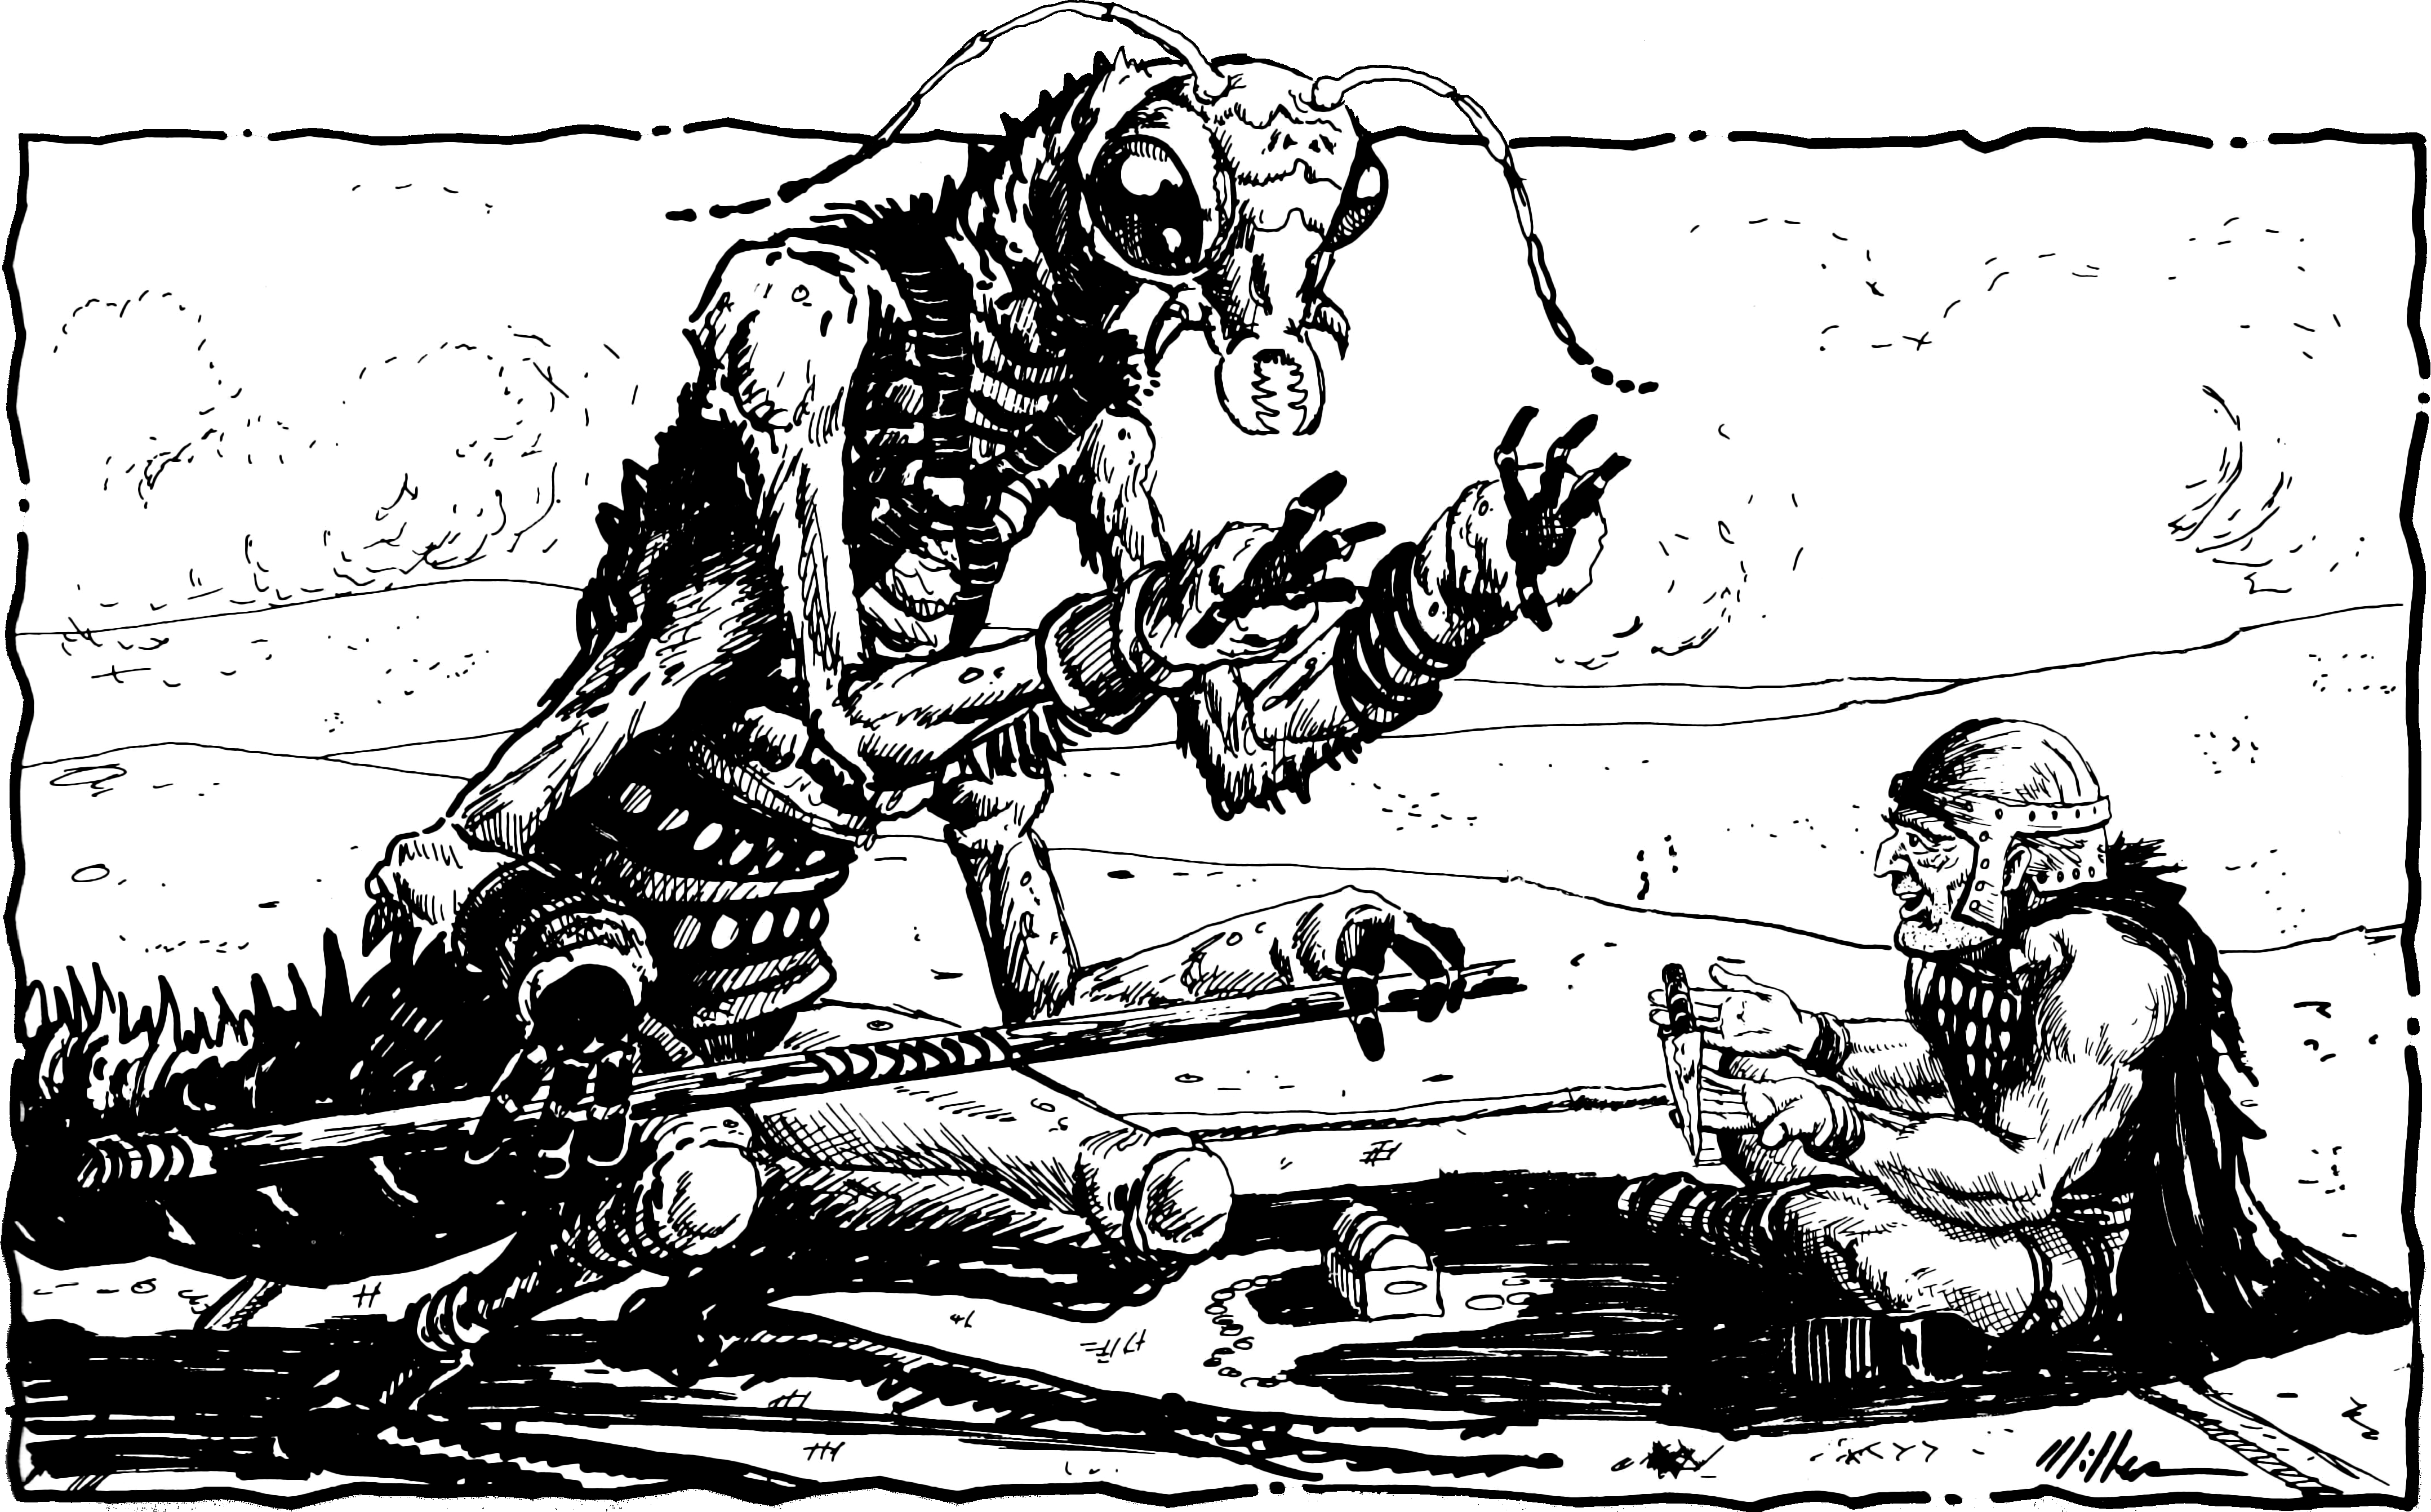
\includegraphics[width=\textwidth]{images/merchant-3.png}
\par\textit{\small\textcopyright Wizards of the Coast, 2020.}
\end{figure*}
\subsection{Documents}
This class of items has a symbolic function, conveying authority or permission. No price is listed for these items, because their value is not inherent.

\textbf{Letter of Marque}: This letter bears the personal mark of the sorcerer‐king, and bestows limited secular authority on the bearer, as if the bearer were a templar. The bearer of a letter of marque gains the authority to contest the actions of templars, using the bearer’s \skill{Diplomacy} check. If the bearer is already a templar, then having the letter as additional authority grants the templar a +4 circumstance check towards authority contest checks. The letter of marque does not grant the authority to Intrude, Requisition, Accuse or Judge, but does grant power to contest such actions by templars. A letter of marque is limited by time. After a specified period (usually one year, and never longer than seven years) the letter loses its effectiveness. A sorcerer‐king can also declare the letter invalid. Forging or fraudulently using a letter of marque is an unpardonable offense that brings a death sentence. Obviously, only the templars and other servants of the sorcerer‐king that issued the letter of marque will honor its terms. A person who is caught with a king’s letter of marque within another sorcerer‐king’s territory will have some explaining to do.

\textbf{Letter of Reprisal}: Like a letter of marque, this letter bears the personal mark of the sorcerer‐king, and bestows limited secular authority on the bearer, as if the bearer were a templar. Unlike a letter of marque, a letter of reprisal has a limited scope to carrying out a specific mission, usually a reprisal or retaliation against a specific group of the King’s enemies, for example, killing or capturing a specific enemy officer, capturing a particular enemy fortress or silt vessel, defiling a stretch of key farmland, or annihilating or enslaving a designated village. Depending on the bearer’s \skill{Diplomacy} ranks, she can Requisition, Intrude, Accuse, Judge, but only if she can show that her request relates to fulfilling her assigned mission. She can attempt to contest the actions of other templars, but takes a $-4$ circumstance penalty on such attempts, since the opposing templars can argue (even if it is not true) that she is acting outside of the scope of the assigned reprisal mission. The $-4$ penalty also applies if templars contest any of her Requisition, Intrude, Accuse, or Judge actions.
\subsectionA{Food, Drink, and Lodging}
Many Athasian travelers are lodged by merchant houses, elemental temples, psionic academies, or family. Adventurers, however, pay for hospitality.

\Table{Food, Drink, and Lodging}{XRR}{
\tableheader Item & \tableheader Cost & \tableheader Weight\\
\TableSubheader{Broy} &&\\
~ Keg (4 liters) & 2 cp & 5 kg\\
~ Mug & 4 bits & \onehalf kg\\
\TableSubheader{Inn stay (per day)} &&\\
~ Good & 2 sp & \\
~ Common & 5 cp & \\
~ Poor & 2 cp & \\
\TableSubheader{Meals (per day)} &&\\
~ Good & 5 bits & \\
~ Common & 3 bits & \\
~ Poor & 1 bit & \\
\TableSubheader{Water} &&\\
~ Keg (4 liters) & 2 bits & 5 kg\\
~ Mug & 1 bd & \onehalf kg\\
}

\textbf{Broy:} Broy is made from fermented kank nectar. Spiced broy and watered-down broy are also available. When served plain, it is potent and foul tasting. However, broy can be served warm and spiced with a pungent herb that disguises its sourness, as well as enhancing its enrapturing powers.

\textbf{Inn:} Poor accommodations at an inn amount to a place on the floor near the hearth. Common accommodations consist of a place on a raised, heated floor, the use of a blanket and a pillow. Good accommodations consist of a small, private room with one bed, some amenities, and a covered chamber pot in the corner.

\textbf{Meals:} Poor meals might be composed of bread, baked turnips, onions, and water. Common meals might consist of bread, chicken stew, carrots, and watered-down ale or wine. Good meals might be composed of bread and pastries, beef, peas, and ale or wine.
\subsectionA{Mounts and Related Gear}

\Table{Mounts and Related Gear}{XRR}{
\tableheader Goods or Services & \tableheader Cost & \tableheader Weight \\
\TableSubheader{Barding} &&\\
~ Medium creature & $\times$2 & $\times$1 \\
~ Large creature & $\times$4 & $\times$2 \\
Bit and bridle & 2 cp & \onehalf kg \\
Feed (per day) & 1 bit & 5 kg \\
\TableSubheader{Mounts} &&\\
~ \TableSubheader{Birds} &&\\
~ Erdland & 25 cp &\\
~ Erdlu & 10 cp &\\
~ \TableSubheader{Reptiles} &&\\
~ Crodlu, riding & 200 cp & \\
~ Crodlu, warmount & 400 cp & \\
~ Inix & 100 cp & \\
~ Mekillot & 200 cp & \\
~ \TableSubheader{Insects} &&\\
~ Kank, herding & 50 cp &\\
~ Kank, riding & 125 cp &\\
~ Kank, warmount & 250 cp &\\
\TableSubheader{Saddle} &&\\
~ Military & 20 cp & 15 kg \\
~ Pack & 5 cp & 7.5 kg \\
~ Riding & 10 cp & 12.5 kg \\
\TableSubheader{Saddle, Exotic} &&\\
~ Military & 60 cp & 20 kg \\
~ Pack & 15 cp & 10 kg \\
~ Riding & 30 cp & 15 kg \\
Saddlebags & 4 cp & 4 kg \\
Stabling (per day) & 5 bits &\\
}

\textbf{Barding, Medium Creature and Large Creature:} Barding is a type of armor that covers the head, neck, chest, body, and possibly legs of a horse or other mount. Barding made of medium or heavy armor provides better protection than light barding, but at the expense of speed. Barding can be made of any of the armor types found on \tabref{Armor and Shields}.

Armor for a horse (a Large nonhumanoid creature) costs four times as much as armor for a human (a Medium humanoid creature) and also weighs twice as much as the armor found on \tabref{Armor and Shields} (see Armor for Unusual Creatures). If the barding is for a pony or other Medium mount, the cost is only double, and the weight is the same as for Medium armor worn by a humanoid. Medium or heavy barding slows a mount that wears it, as shown on the table below.

Flying mounts can't fly in medium or heavy barding.

Removing and fitting barding takes five times as long as the figures given on \tabref{Donning Armor}. A barded animal cannot be used to carry any load other than the rider and normal saddlebags.

\Table{Barding}{XCCC}{
 & \multicolumn{3}{c}{\tableheader Base Speed}\\
\cmidrule[0.5pt]{2-4}
\tableheader Barding & \tableheader (12 m) & \tableheader (15 m) & \tableheader (18 m)\\
Medium & 9 m & 10.5 m & 12 m\\
Heavy & 9 m\footnotemark[1] & 10.5 m\footnotemark[1] & 12 m\footnotemark[1]\\

\TableNote{4}{1 A mount wearing heavy armor moves at only triple its normal speed when running instead of quadruple.}\\
}

\textbf{Crodlu:} A crodlu is a large bipedal lizard mount, resembling a scaled ostrich. A crodlu is appropriate as a mount for a Medium humanoid creature. Crodlu are hard to control in battle, while war crodlu can be ridden into battle easily. Crodlu benefit from stabling, can wear barding, and require feed like normal mounts.

\textbf{Erdland:} These creatures are large, flightless birds used as mounts or to pull caravans. They weigh around 2 tons and can stand up to 4.5 meters tall. An erdland is appropriate as a mount for a Medium humanoid creature. Erdlands can be ridden into battle easily. Erdlands benefit from stabling, can wear barding, and require feed like normal mounts.

\textbf{Erdlu:} Erdlus are a smaller variety of erdland, mostly used as herd beasts. They stand 2.1 meters tall and weigh around 100 kg. An erdlu is appropriate as a mount for a Medium humanoid creature. Erdlus are hard to control in battle. Erdlus benefit from stabling, can wear barding, and require feed like normal mounts.

\textbf{Feed:} Crodlus, erdlands, erdlus, inixes require feeding. Mekillots require eight times more than normal mounts.

\textbf{Inix:} The inix is a large, 5.5-meter long reptile commonly used for riding and as a beast of burden. An inix is appropriate as a mount for a Medium or Large humanoid creature. Inixes can be ridden into battle easily. Inixes benefit from stabling, can wear custom barding (specially constructed, adding an additional 50\% to the price), and require feed like normal mounts.

\textbf{Kank:} A kank is a large, 2.4-meter long insect, commonly used as a personal mount. These insects cannot be used as food, for their meat smells atrocious, but they produce highly nutritious globules of honey. A kank is appropriate as a mount for a Medium humanoid creature. Kanks are hard to control in battle. Kanks benefit from stabling, cannot wear barding, and do not require feeding.

\textbf{Mekillot:} A mekillot is a huge, 3,000-kg. lizard, used for hauling large cargo or serving as transportation for troops. These beasts are hard to control in combat and usually require a psionic handler. Mekillots benefit from stabling, can wear barding, and require feed eight times more than a normal mount.

\textbf{Saddle, Exotic:} An exotic saddle is like a normal saddle of the same sort except that it is designed for an unusual mount. Exotic saddles come in military, pack, and riding styles.

\textbf{Saddle, Military:} A military saddle braces the rider, providing advantage on \skill{Ride} checks related to staying in the saddle. If you're knocked unconscious while in a military saddle, you have a 75\% chance to stay in the saddle (compared to 50\% for a riding saddle).

\textbf{Saddle, Pack:} A pack saddle holds gear and supplies, but not a rider. It holds as much gear as the mount can carry.

\textbf{Saddle, Riding:} The standard riding saddle supports a rider.

\clearpage
\begin{figure}[t!]
\centering
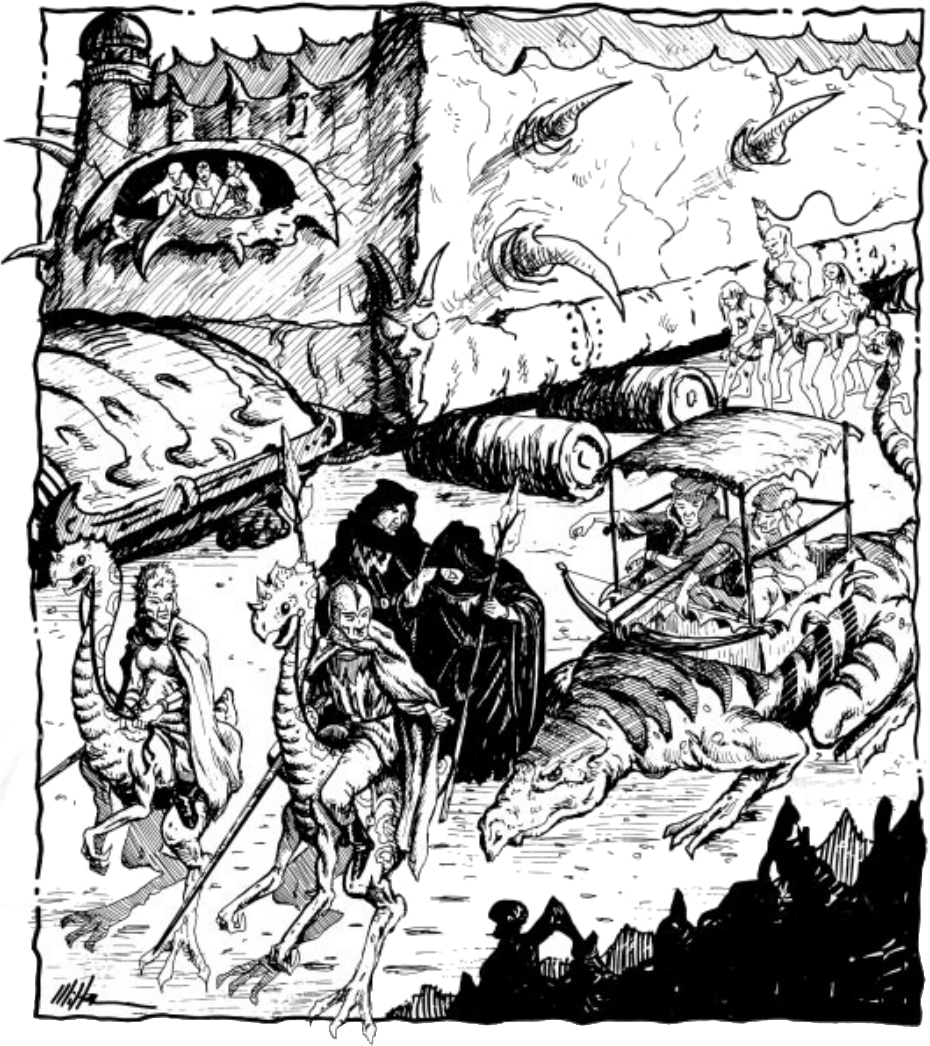
\includegraphics[width=\columnwidth]{images/caravan-3.png}
\par\textit{\small\textcopyright Wizards of the Coast, 2020.}
\end{figure}
\subsection{Transport}
Sometimes it is too hard or too dangerous to ride a kank---you'll need some other form of transportation. Some vehicles, such as the chariot and howdah, are moved by muscle power. The \skill{Handle Animal} skill is used only if that power comes from a team of draft animals. When the team consists of creatures with Intelligence scores of 3 or higher, the operative skill is \skill{Diplomacy}. When they are slaves or forced labor, the operative skill is \skill{Intimidate}.

\Table{Transport}{Xr{2cm}}{
\tableheader Transport & \tableheader Cost\\
Chariot, two-person, transport & 50 cp \\
Chariot, two-person, war & 125 cp \\
Chariot, four-person, war & 250 cp \\
Howdah, inix & 10 cp \\
Howdah, inix, war & 100 cp \\
Howdah, mekillot & 20 cp \\
Howdah, mekillot, war & 500 cp \\
Wagon, open, 500 kg capacity & 20 cp \\
Wagon, open, 1,250 kg capacity & 35 cp \\
Wagon, open, 2,500 kg capacity & 50 cp \\
Wagon, open, 5,000 kg capacity & 100 cp \\
Wagon, enclosed, 500 kg capacity & 40 cp \\
Wagon, enclosed, 1,250 kg capacity & 70 cp \\
Wagon, enclosed, 2,500 kg capacity & 100 cp \\
Wagon, enclosed, 5,000 kg capacity & 200 cp \\
Wagon, armored caravan & 1,000 cp \\
}

\textbf{Chariot}: A chariot is a two‐wheeled vehicle used for transportation, racing, war and processions. Transport chariots are very small and simple, requiring only a single animal to draw it. A war chariot built for two riders is slightly larger, but significantly better constructed. Generally one person will drive the chariot while the other uses a bow or other ranged weapon. A war chariot built for four is much larger than the other two kinds of chariots and requires at least two mounts to drive it. A war chariot offers cover to its occupants.

\textbf{Howdah}: A howdah is an enclosure mounted on a riding animal containing space for one or more persons. Howdahs can be fitted on inix or mekillots, and provide shade and cover from the elements. An inix howdah usually has room for only one person, though the war howdah, built much stronger, can hold four. A mekillot howdah can hold one or two persons, but a war howdah is much bigger, consisting of two levels and holding up to sixteen warriors.

\textbf{Wagon}: Wagons are an essential part of Athasian economy, as they facilitate the caravans that make life in the wastes possible. Open wagons are basic, open–topped wagons that can carry a certain amount of cargo. As Athasian wagons are built using little or no metal, there’s a limit to how much cargo they can carry. Open wagons generally require two beasts to draw them, but sometimes a single erdland will work.

\textit{Enclosed wagons}: They are more commonly used to transport people or fragile cargo that would otherwise be damaged by exposure to the elements.

\textit{Armored wagons}: They are primarily used by caravans traveling through areas plagued by dangerous monsters or raiders. It is an enclosed wagon with agafari wood used to strengthen the wagon throughout. There are also mount points for fixed crossbows on each side of that wagon that can swivel 180 degrees. Anyone using the crossbows or firing out of the rear of the wagon (when it is open) receives cover. Armored wagons require at least four smaller mounts to draw it, two inixes or one mekillot.

\subsectionA{Services}

\Table{Services}{lR}{
\tableheader Services & \tableheader Cost\\
Messenger         & 1 bit/km\\
Road or gate toll & 1 bit\\

\multicolumn{2}{l}{\TableSubheader{Hirelings, Military}}\\
Archer              & 1 bit/day  \\
Cavalry, heavy      & 3 bits/day \\
Cavalry, light      & 1 bit/day  \\
Crossbowman         & 5 bd/day   \\
Engineer            & 5 cp/day   \\
Infantry, heavy     & 5 bd/day   \\
Infantry, light     & 2 bd/day   \\
Infantry, irregular & 1 bd/day   \\

\multicolumn{2}{l}{\TableSubheader{Hirelings, Civilian}}\\
Draqoman                        & Level in cp/day \\
Craftsman\footnotemark[1]       & 1 bit/day      \\
Professional\footnotemark[2]    & 5 bd/day       \\
Specialist\footnotemark[3]      & 3 bits/day     \\
Spellcaster                     & 5 bits/day     \\
Unskilled labor\footnotemark[4] & 2 bd/day       \\


\multicolumn{2}{l}{\TableSubheader{Manifesting}}\\
Power, 1st--level & Manifester level $\times$ 10 cp\footnotemark[5]\\
Power, 2nd--level & Manifester level $\times$ 20 cp\footnotemark[5]\\
Power, 3rd--level & Manifester level $\times$ 30 cp\footnotemark[5]\\
Power, 4th--level & Manifester level $\times$ 40 cp\footnotemark[5]\\
Power, 5th--level & Manifester level $\times$ 50 cp\footnotemark[5]\\
Power, 6th--level & Manifester level $\times$ 60 cp\footnotemark[5]\\
Power, 7th--level & Manifester level $\times$ 70 cp\footnotemark[5]\\
Power, 8th--level & Manifester level $\times$ 80 cp\footnotemark[5]\\
Power, 9th--level & Manifester level $\times$ 90 cp\footnotemark[5]\\

\multicolumn{2}{l}{\TableSubheader{Spellcasting}}\\
Spell,   0--level & Caster level $\times$  5 sp\footnotemark[5]\footnotemark[6]\\
Spell, 1st--level & Caster level $\times$ 10 sp\footnotemark[5]\footnotemark[6]\\
Spell, 2nd--level & Caster level $\times$ 20 sp\footnotemark[5]\footnotemark[6]\\
Spell, 3rd--level & Caster level $\times$ 30 sp\footnotemark[5]\footnotemark[6]\\
Spell, 4th--level & Caster level $\times$ 40 sp\footnotemark[5]\footnotemark[6]\\
Spell, 5th--level & Caster level $\times$ 50 sp\footnotemark[5]\footnotemark[6]\\
Spell, 6th--level & Caster level $\times$ 60 sp\footnotemark[5]\footnotemark[6]\\
Spell, 7th--level & Caster level $\times$ 70 sp\footnotemark[5]\footnotemark[6]\\
Spell, 8th--level & Caster level $\times$ 80 sp\footnotemark[5]\footnotemark[6]\\
Spell, 9th--level & Caster level $\times$ 90 sp\footnotemark[5]\footnotemark[6]\\

\TableNote{2}{1 Any \skill{Craft} skill available.}\\
\TableNote{2}{2 Any \skill{Profession} skill available.}\\
\TableNote{2}{3 Any skill, other than Craft and Profession.}\\
\TableNote{2}{4 Jobs that do not require associated skills.}\\
\TableNote{2}{5 See its description for additional costs. If the additional costs put the total cost above 3,000 cp, that service is not generally available.}\\
\TableNote{2}{6 Spellcasting is considered high treason and spellcasters are not comfortable offering their services.}\\
}

Sometimes the best solution for a problem is to hire someone else to take care of it. Spellcasting, unless divine, is rarely, if ever, for sale on Athas. However, the manifesting of psionic powers for cash is much more common.

\textbf{Archer:} A 2nd-level fighter specialized in longbows, weilding a composite longbow (Str +2), and wearing studded leather and a buckler.

\textbf{Cavalry, Heavy:} A 2nd-level fighter wearing scale mail, and wielding a lance two-handed. They mount a heavy crodlu wearing a scale mail, as well.

\textbf{Cavalry, Light:} A 1st-level fighter wearing a studded leather and a wooden shield, and wielding a lance. They mount a light crodlu with no armor.

\textbf{Craftsman:} Usually a 2nd-level settler, but they can be of any class. This pays for any \skill{Craft} check of DC 20 or lower. Higher DC checks double the price for each 5 points of difference. 

\textbf{Crossbowman:} A 1st-level fighter specialized in crossbows, weilding a composite heavy crossbow (Str +4), and wearing studded scale mail and a tower shield.

\textbf{Draqoman:} A bard of 6th or higher level with at least one contact (see Alternative Class Features). Their wages depends on the bard's level and are the default price for skill contacts. If the draqoman has different types of contact, then they might double the price.

\textbf{Engineer:} A 5th-level fighter with 8 ranks of \skill{Knowledge} (warcraft) and a martial prowess that depend on this skill. They are equipped with \emph{breastplate +1} and a \emph{tower shield +1}. Although a military engineer has combat capabilities, their function is to oversee construction of siege engines and of static defenses.

\textbf{Infantry, Heavy:} A 2nd-level fighter, wearing a half-plate and tower shield, wielding a one-handed weapon. 

\textbf{Infantry, Light:} A 1st-level fighter, specialized either in spear and shields, or longswords. Light infantry usually wears studded leather, but caravan's infantry wear caravan armor.

\textbf{Infantry, Irregular:} A 2nd-level barbarian or gladiator. Their specialization is atypical, and they typically use gladiator armor or shell armor.

\textbf{Messenger:} This entry includes mounted messengers and runners. Those willing to carry a message to a place they were going anyway may ask for only half the indicated amount.

\textbf{Power:} The indicated amount is how much it costs to get a manifester to manifest a power for you. This cost assumes that you can go to the manifester and have the power manifested at his or her convenience. If you want to bring the manifester somewhere to manifest a power you need to negotiate with the manifester, otherwise the default answer is no.

The cost given is for a power with no XP cost. If the power has an XP cost, add 5 cp per XP lost.

Furthermore, if a power has dangerous consequences, the manifester will certainly require proof that you can and will pay for dealing with any such consequences (that is, assuming that the manifester even agrees to manifest such a power, which isn't certain). In the case of powers that transport the manifester and characters over a distance, you will likely have to pay for two manifestations of the power, even if you aren't returning with the manifester.

In addition, not every town or village has a manifester of sufficient level to manifest any power. In general, you must travel to a small town (or larger settlement) to be reasonably assured of finding a manifester capable of manifesting 1st--level powers, a large town for 2nd--level powers, a small city for 3rd-- or 4th--level powers, a large city for 5th-- or 6th--level powers, and a metropolis for 7th-- or 8th--level powers. Even a metropolis isn't guaranteed to have a local manifester able to cast 9th--level powers.

\textbf{Professional:} Usually a 2nd-level settler, but they can be of any class. This pays for any \skill{Profession} check of DC 20 or lower. Higher DC checks double the price for each 5 points of difference.

\textbf{Road or Gate Toll:} A toll is sometimes charged to cross a well-trodden, well-kept, and well-guarded road to pay for patrols on it and for its upkeep. Occasionally, a large walled city charges a toll to enter or exit (or sometimes just to enter).

\textbf{Specialist:} A 2nd-level NPC with \feat{Skill Focus} on the corresponding skill speciality, who can deliver a skill check of DC 20. Scouts are usually hired for \skill{Knowledge} (geography), \skill{Spot}, or \skill{Survival}. Thieves for \skill{Disable Device}, \skill{Forgery}, \skill{Open Lock}, \skill{Search}, or \skill{Sleight of Hand}. Bards for \skill{Appraise}, \skill{Diplomacy}, or \skill{Perform}. Wizards for \skill{Decipher Script}, any \skill{Knowledge}, or \skill{Spellcraft}. These are guidelines, but the wages are the same for any class.

\textbf{Spell:} The indicated amount is how much it costs to get a spellcaster to cast a spell for you. This cost assumes that you can go to the spellcaster and have the spell cast at his or her convenience (generally at least 24 hours later, so that the spellcaster has time to prepare the spell in question). If you want to bring the spellcaster somewhere to cast a spell you need to negotiate with him or her, and the default answer is no.

The cost given is for a spell with no cost for a material component or focus component and no XP cost. If the spell includes a material component, add the cost of that component to the cost of the spell.

If the spell has a focus component (other than a divine focus), add 1/10 the cost of that focus to the cost of the spell. If the spell has an XP cost, add 5 cp per XP lost.

Furthermore, if a spell has dangerous consequences, the spellcaster will certainly require proof that you can and will pay for dealing with any such consequences (that is, assuming that the spellcaster even agrees to cast such a spell, which isn't certain). In the case of spells that transport the caster and characters over a distance, you will likely have to pay for two castings of the spell, even if you aren't returning with the caster.

In addition, not every town or village has a spellcaster of sufficient level to cast any spell. In general, you must travel to a small town (or larger settlement) to be reasonably assured of finding a spellcaster capable of casting 1st--level spells, a large town for 2nd--level spells, a small city for 3rd-- or 4th--level spells, a large city for 5th-- or 6th--level spells, and a metropolis for 7th-- or 8th--level spells. Even a metropolis isn't guaranteed to have a local spellcaster able to cast 9th--level spells.

\textbf{Spellcaster:} A 3rd-level cleric or wizard. These wages do not pay for expensive material components, which must be given by the employer.

\textbf{Unskilled Labor:} Any job that a freeman might do that does not require a skill check.


\section{Siege Engines}
Siege engines are large weapons, temporary structures, or pieces of equipment traditionally used in besieging a castle or fortress.

\Table{Siege Engines}{lR*4C}{
  \tableheader Item
& \tableheader Cost
& \tableheader Damage
& \tableheader Critical
& \tableheader Range Increment
& \tableheader Typical Crew \\
Catapult, heavy &  80 sp & 6d6 & & 60 m\footnotemark[1] & 4 \\
Catapult, light &  55 sp & 4d6 & & 45 m\footnotemark[1] & 2 \\
Ballista        &  50 sp & 3d8 & 19--20 & 36 m & 1 \\
Ram             & 100 sp & 3d8\footnotemark[2] & & & 10 \\
Siege tower     & 200 sp & & & & 20 \\
Mekillot ram    & 300 sp & 6d8 & & & 8 \\
\TableNote{6}{1 30 m minimum.}\\
\TableNote{6}{2 See description for special rules.}\\
}

\Figure*{t}{images/mekillot-ram.png}

\BigTableBottom{Catapult Attack Modifiers}{XR}{
\tableheader Condition & \tableheader Modifier\\
No line of sight to target square & $-6$\\
Successive shots (crew can see where most recent misses landed) & Cumulative +2 per previous miss (maximum +10)\\
Successive shots (crew can't see where most recent misses landed, but observer is providing feedback) & Cumulative +1 per previous miss (maximum +5)\\
}

\textbf{Catapult, Heavy:} A heavy catapult is a massive engine capable of throwing rocks or heavy objects with great force. Because the catapult throws its payload in a high arc, it can hit squares out of its line of sight. To fire a heavy catapult, the crew chief makes a special check against DC 15 using only his base attack bonus, Intelligence modifier, range increment penalty, and the appropriate modifiers from the lower section of \tabref{Catapult Attack Modifiers}. If the check succeeds, the catapult stone hits the square the catapult was aimed at, dealing the indicated damage to any object or character in the square. Characters who succeed on a DC 15 Reflex save take half damage. Once a catapult stone hits a square, subsequent shots hit the same square unless the catapult is reaimed or the wind changes direction or speed.

If a catapult stone misses, roll 1d8 to determine where it lands. This determines the misdirection of the throw, with 1 being back toward the catapult and 2 through 8 counting clockwise around the target square. Then, count 3 squares away from the target square for every range increment of the attack.

Loading a catapult requires a series of full-round actions. It takes a DC 15 Strength check to winch the throwing arm down; most catapults have wheels to allow up to two crew members to use the aid another action, assisting the main winch operator. A DC 15 \skill{Profession} (siege engineer) check latches the arm into place, and then another DC 15 \skill{Profession} (siege engineer) check loads the catapult ammunition. It takes four full-round actions to reaim a heavy catapult (multiple crew members can perform these full-round actions in the same round, so it would take a crew of four only 1 round to reaim the catapult).

A heavy catapult takes up a space 4.5 meters across.

\textbf{Catapult, Light:} This is a smaller, lighter version of the heavy catapult. It functions as the heavy catapult, except that it takes a DC 10 Strength check to winch the arm into place, and only two full-round actions are required to reaim the catapult.

A light catapult takes up a space 3 meters across.

\textbf{Ballista:} A ballista is essentially a Huge heavy crossbow fixed in place. Its size makes it hard for most creatures to aim it. Thus, a Medium creature takes a $-4$ penalty on attack rolls when using a ballista, and a Small creature takes a $-6$ penalty. It takes a creature smaller than Large two full-round actions to reload the ballista after firing.

A ballista takes up a space 1.5 meter across.

\textbf{Mekillot Ram:} This 15-meter war machine has a live mekillot encased within a twelve-wheeled car. The structure has an upper and central deck, with a 3-meter spiked ram at the front, a rear tower, and a heavy catapult on the upper deck. The ram section has reinforced chitin plates, while the ram itself is carved to a point. It can hold up to 64 soldiers, 24 soldiers on the upper deck and 40 in the central deck. These rams also have harness for 40 slaves to help push the vehicle.

In order to make the equivalent of a swing of a ram, the mekillot must take a standard action to charge against the AC of the construction, moving up to 6 meters, and applying disadvantage for the lack of proficiency. In addition to the damage given on \tabref{Siege Engines}, each slave helping push the ram adds their Strength modifier to the ram's damage.

The ram requires a crew chief, two drivers to tend the mekillot, a lookout, and the four-person crew for the heavy catapult. Drivers use psionic or magical means to contact the lookout to steer the vehicle. The mekillot cannot be removed from the ram, and must be fed and watered within its shell.

A mekillot ram takes up a 15-meter-by-7.5-meter space. The mekillot can push the ram at a speed of 6 meters (and a mekillot ram can't run). With the 40 slaves helping push the vehicle, they increase the vehicle's speed to 12 meters (it still can't run). This is usually only done in battle, and the mekillot carries the ram alone during travel.

\textbf{Ram:} This heavy pole is sometimes suspended from a movable scaffold that allows the crew to swing it back and forth against objects. As a full-round action, the character closest to the front of the ram makes an attack roll against the AC of the construction, applying disadvantage for lack of proficiency. (It's not possible to be proficient with this device.) In addition to the damage given on \tabref{Siege Engines}, up to nine other characters holding the ram can add their Strength modifier to the ram's damage, if they devote an attack action to doing so. It takes at least one Huge or larger creature, two Large creatures, four Medium-size creatures, or eight Small creatures to swing a ram. (Tiny or smaller creatures can't use a ram.)

A ram is typically 9 meters long. In a battle, the creatures wielding the ram stand in two adjacent columns of equal length, with the ram between them.

\textbf{Siege Tower:} This device is a massive wooden tower on wheels or rollers that can be rolled up against a wall to allow attackers to scale the tower and thus to get to the top of the wall with cover. The wooden walls are usually 30 centimeters thick.

A typical siege tower takes up a space 4.5 meters across. The creatures inside push it at a speed of 3 meters (and a siege tower can't run). The eight creatures pushing on the ground floor have total cover, and those on higher floors get improved cover and can fire through arrow slits.


\section{Special Materials}
A number of exotic materials can be found in the wilds and underground of the Tablelands and beyond, in addition to the more mundane ones. These substances have innate special properties. If you make a suit of armor or weapon out of more than one special material, you get the benefit of only the most prevalent material. However, you can build a double weapon with each head made of a different special material.

\subsection{Special Weapons Materials}
Each of the special materials described below has a definite game effect. Some creatures have damage reduction based on their creature type or core concept. Some are resistant to all but a special type of damage, such as that dealt by evil-aligned weapons or bludgeoning weapons. Others are vulnerable to weapons of a particular material. Characters may choose to carry several different types of weapons, depending upon the campaign and types of creatures they most commonly encounter.

\Table{Special Materials Cost Modifiers}{Xr{2.6cm}}{
\tableheader Type of Item & \tableheader Item Cost Modifier\\
\TableSubheader{Adamantine (dwarven steel)} &\\
Ammunition & +60 gp\\
Weapon & +3,000 gp\\
Shield & +2,000 gp\\
Light armor & +5,000 gp\\
Medium armor & +10,000 gp\\
Heavy armor & +15,000 gp\\

\TableSubheader{Agafari} &\\
Any wooden item & $\star$ + 20 cp per kg\\

\TableSubheader{Crystal, deep} &\\
Any weapon & +1,000 cp\\

\TableSubheader{Crystal, living} &\\
Ammunition & +250 cp\\
Light weapon & +750 gp\\
One-handed weapon, or one head of a double weapon & +1,000 gp\\
Two-handed weapon, or both heads of a double weapon & +1,500 gp\\
Light armor & +2,000 cp\\
Medium armor & +5,000 cp\\
Heavy armor & +9,000 cp\\

\TableSubheader{Crystal, mundane} &\\
Any armor, shield, or weapon & $\star$\\

\TableSubheader{Dasl} &\\
Any weapon & $\times$10\\

\TableSubheader{Drakehide} &\\
Any armor or shield & $\star$ $\times$ 2\\

\TableSubheader{Drake Ivory} &\\
Any weapon & $\times$2\\

\TableSubheader{Iron} &\\
Any armor, shield, or weapon & $\times$100\\

\TableSubheader{Silver, alchemical} &\\
Ammunition & +2 gp\\
Light weapon & +20 gp\\
One-handed weapon, or one head of a double weapon & +90 gp\\
Two-handed weapon, or both heads of a double weapon & +180 gp\\

\TableNote{2}{$\star$ Masterwork price}
}

\textbf{Adamantine}: While weapons and armor made from adamantine, also called ``dwarven steel'', can be found on Athas, they are quite rare. Nearly all items made from adamantine are relics from a long past age, scavenged from ruins by elves and treasure hunters. Raw adamantine cannot be bought on the market, and weapons and armor constructed from adamantine are considered priceless relics.

This ultrahard metal adds to the quality of a weapon or suit of armor. Weapons fashioned from adamantine have a natural ability to bypass hardness when sundering weapons or attacking objects, ignoring hardness less than 20. Armor made from adamantine grants its wearer damage reduction of 1/-- if it's light armor, 2/-- if it's medium armor, and 3/-- if it's heavy armor. Adamantine is so costly that weapons and armor made from it are always of masterwork quality; the masterwork cost is included in the prices. Thus, adamantine weapons and ammunition have a +1 enhancement bonus on attack rolls, and the armor check penalty of adamantine armor is lessened by 1 compared to ordinary armor of its type. Items without metal parts cannot be made from adamantine. An arrow could be made of adamantine, but a quarterstaff could not.

Only weapons, armor, and shields normally made of metal can be fashioned from adamantine. Weapons, armor and shields normally made of steel that are made of adamantine have one-third more hit points than normal. Adamantine has 40 hit points per inch of thickness and hardness 20.

\textbf{Agafari}: This rare magic wood is as hard as normal wood but very light. Any wooden or mostly wooden item (such as a bow, an arrow, or a spear) made from agadari is considered a masterwork item and weighs only half as much as a normal wooden item of that type. Items not normally made of wood or only partially of wood (such as a battleaxe or a mace) either cannot be made from agadari or do not gain any special benefit from being made of agadari. The armor check penalty of a agadari shield is lessened by 2 compared to an ordinary shield of its type. To determine the price of a agadari item, use the original weight but add 20 cp per kilogram to the price of a masterwork version of that item.

For weapons affected by the inferior material rule, agafari is considered an inferior material.

Agafari has 10 hit points per inch of thickness and hardness 5.

\textbf{Crystal, Deep}: Deep crystal is crystal of above-average quality found at the hearts of large veins or deposits of mundane crystal (see below). Deep crystal is renowned for its strength and its psionically resonant nature. Mundane crystal is used for many items of psionic manufacture, such as dorjes, power stones, and psicrystals. Deep crystal is a better grade.

While a weapon made of deep crystal is no different from a mundane crystal weapon for a nonpsionic character, a psionic wielder of a deep crystal weapon can focus psionic power through it, increasing the damage that weapon deals. As a free action that does not provoke attacks of opportunity, the wielder can channel psionic power into a melee weapon or ranged weapon made of deep crystal. For 2 power points, the deep crystal weapon deals an extra 2d6 points of damage. The weapon will stay charged for 1 minute or until it scores its next hit. Bows, crossbows, and slings bestow this power on their ammunition. All missile weapons lose this effect if they miss. However, they may be recovered and charged again.

Any weapon made of deep crystal costs 1,000 cp more than its noncrystal counterpart. Any item could potentially be made out of deep crystal. Because deep crystal armor is considered to be made out of metal, druids cannot wear it.

Deep crystal has 30 hit points per inch of thickness and hardness 10.

\textbf{Crystal, Living}: Living crystal is crystal of above-average quality renowned for its strength and its psionically-resonant nature. It is actually two different materials: the crystalline web material of a crystal spider used in making weapons, and the tissue of the crystal spider itself for making armor. The freshly-taken material must be treated within a day of its extraction by channeling psionic power into it, preserving its inherent psionic nature. One power point is required for every treated pound of material.

While a weapon made of living crystal is no different from a mundane crystal weapon (see below) for a nonpsionic character, a psionic wielder of a living crystal weapon can focus psionic power through it, increasing the damage that weapon deals. As a free action that does not provoke attacks of opportunity, and with the expediture of his psionic focus, the wielder can channel psionic power into a melee weapon or ranged weapon made of living crystal. For 2 power points, the living crystal weapon deals an extra 2d6 points of damage. The weapon will stay charged for 1 minute or until it scores its next hit. Bows, crossbows, and slings bestow this power on their ammunition. All missile weapons lose this effect if they miss. However, they may be recovered and charged again. For weapons affected by the inferior material rule, living crystal is considered inferior.

Armor made of living crystal is no different than metal armor for a nonpsionic character, but a psionic wearer of living crystal armor can focus psionic power through it, gaining an amount of damage reduction in the process. As a free action that does not provoke attacks of opportunity, and with the expediture of his psionic focus, the wearer can channel psionic power into armor made of living crystal. For 2 power points, the living crystal armor confers to the wearer damage reduction 5/metal. The armor will stay charged for 1 minute or until a hit is scored on it, whether or not the damage reduction applies to that particular hit. Unlike metal armor, living crystal armor isn't considered made of metal so druids can wear it without penalty.

Living crystal has 15 hit points per inch of thickness and hardness 8.

\textbf{Crystal, Mundane}: Mundane crystal can be used in place of metal in weapons or armor, using a special forging process. The fortified crystal possesses the properties of a similar masterwork steel weapon or armor, except for visual appearance.

Weapons and armor made of mundane crystal cost the same amount to make as their masterwork counterparts. Any item could potentially be made with mundane crystal. Because mundane crystal armor is considered to be made out of metal, druids cannot wear it.

Mundane crystal properly forged has 25 hit points per inch of thickness and a hardness of 8.

\textbf{Dasl}: Dasl is a special kind of crystalline material created by thri-kreen and often used to manufacture their weapons. An item made from dasl is treated as if it was made from iron and is not considered to be made from inferior materials. However, for purposes of harming creatures with damage reduction, a dasl weapon is not treated as being made from metal. An item made from dasl costs ten times what it normally would. Thus, a dasl chatkcha costs 200 cp instead of the 20 cp a stone or bone chatkcha would.

Dasl has a 15 hit points per inch of thickness and hardness 7.

\textbf{Drakehide}: The hide of a drake is of such value that most sorcerer-kings forbid their sale. They have instructed templars to confiscate any such items that appear in the market in the name of their sorcerer-king. Because drakes are so rare it is easy for templars to claim the item was stolen from the sorcerer-king and have the seller put to death. Elves, of course, defy these edicts at every turn, and make a fair profit selling drake materials while just one step ahead of their templar pursuers.

Armorsmiths can work with the hides of drakes to produce armor or shields of masterwork quality. One drake produces enough hide for four suits of hide armor, three suits of banded mail, two suits of half-plate, or one suit of full plate for a Medium creature. Enough hide is available to produce a small or large masterwork shield in addition to the armor.

Because dragonhide armor isn't made of metal, druids can wear it without penalty.

Drakehide armor costs double what masterwork armor of that type ordinarily costs, but it takes no longer to make than ordinary armor of that type.

Drakehide has 10 hit points per inch of thickness and hardness 10.

\textbf{Drake Ivory}: Drake ivory is extraordinarily strong and easy to work compared to the bone that most Athasian weaponsmiths use. Since it can only be obtained from the claws and teeth of deadly drakes, it is rare, expensive, and forbidden (see drakehide, above).

Weapons made from drake ivory cost an additional 2,000 cp to enchant. Weapons crafted from drake ivory cost twice what they normally would. A double weapon that is only half crafted using drake ivory increases its cost by 50\%.

Drake ivory has 30 hit points per inch of thickness and hardness 10.

% Giant Hair: Giant hair is very strong and frequently woven together to form a very strong cord. While sometimes used in armor, it is most frequently used to create rope. This rope costs 50 cp for 15 meters, has a hardness of 5 and 2 hp per inch of thickness

\textbf{Iron}: Iron (and most other metals) is rare on Athas, but weapons and armor made of iron can still be found. In all of the city-states, there are at least a few craftsmen that are able to work iron. The only fresh source of iron is the mines in the city-state of Tyr. Many of the iron weapons and armor available for sale have been scavenged from ruins. Weapons made of iron (including iron-based compounds like steel) can bypass the damage reduction possessed by some Athasian monsters. Iron-based items cost 100 times what they normally would.

Iron has 30 hit points per inch of thickness and hardness 10.

\textbf{Silver, Alchemical}: The process of binding silver to weapons has been greatly refined on Athas. Very little silver is actually needed in the process, and it can be bound to weapons crafted from dasl, obsidian and bone, as well as those made from iron.

A complex process involving metallurgy and alchemy can bond silver to a weapon made of steel so that it bypasses the damage reduction of creatures such as lycanthropes.

On a successful attack with a silvered weapon, the wielder takes a $-1$ penalty on the damage roll (with the usual minimum of 1 point of damage). The alchemical silvering process can't be applied to nonmetal items, and it doesn't work on rare metals such as adamantine, cold iron, and mithral.

Alchemical silver has 10 hit points per inch of thickness and hardness 8.

\Chapter{Items of Power}
{A village can prosper or die with the utterance of a single syllable. Toxic water can be purified or deadly plague can be unleashed by the power of nature contained in a clay tablet or bone fetish. A ring could save a dying man or protect the land from being reduced to ash by defilers, or help destroy them both. A crystal could dominate the will of its possessor, or serve as a storage of psychic energy. Even mundane looking objects can contain highly sought after power, which makes every item a potential treasure or curse.}{The Oracle, Blue Shrine Scrolls}

\Capitalize{I}{tems} of power come in two types: magic items and psionic items. Magic items are divided into categories: armor, weapons, potions, rings, rods, scrolls, staffs, wands, and wondrous items. In addition, some magic items are cursed. Psionic items are divided into: cognizance crystals, intelligent items, and psionic tattoos.

Finally, a few items of power are of such rarity and power that they are considered to belong to a category of their own: artifacts. Artifacts are classified in turn as minor (extremely rare but not one-of-a-kind items) or major (each one unique and extremely potent).

\textbf{Armor and shields:} Magic armor (including shields) offers improved, magical protection to the wearer. Some of these items confer abilities beyond a benefit to Armor Class.

\textbf{Weapons:} Magic weapons are created with a variety of combat powers and almost always improve the attack and damage rolls of the wielder as well.

\textbf{Potions:} A potion is an elixir concocted with a spell-like effect that affects only the drinker.

\textbf{Rings:} A ring is a circular metal band worn on the finger (no more than two rings per wearer) that has a spell-like power (often a constant effect that affects the wearer).

\textbf{Rods:} A rod is a scepter-like item with a special power unlike that of any known spell.

\textbf{Scrolls:} A scroll is a spell magically inscribed onto paper or parchment so that it can be used later.

\textbf{Staffs:} A staff has a number of different (but often related) spell effects. A newly created staff has 50 charges, and each use of the staff depletes one or more of those charges.

\textbf{Wands:} A wand is a short stick imbued with the power to cast a specific spell. A newly created wand has 50 charges, and each use of the wand depletes one of those charges.

\textbf{Wondrous Items:} These objects include magic jewelry, tools, books, clothing, and much more.

\textbf{Cognizance Crystals:} A cognizance crystal resembles a piece of elaborate jewelry. It stores power points that can be used later by any psionic creature or character.

\textbf{Intelligent Items:} An intelligent item is an item with its own will and psionic powers. It can be any non-consumable item, such as jewelry, rod, armor or weapon.

\textbf{Psionic Tattoos:} A psionic tattoo is a psionic power permanently scribed into the wearer's skin.

\Figure*{t}{images/weapons-1.png}

\section{Handling Magic Items}

\subsection{Identifying Items}
\textbf{Trial and Error:} Close study of an item might provide some information. A DC 15 (or maybe 20) \skill{Search} check should reveal a clue for how the item works, such as a tiny command word etched inside a ring or feather motifs that hint the ability to fly.

You might also permit a character to attempt a DC 30 \skill{Spellcraft} check or \skill{Knowledge} (arcana) check to determine if she can attune herself with the item's power or if she remembers reading of it once in her studies.

\textbf{Spells:} The easiest way to discern whether an object is magical is to use \spell{detect magic}. A character can focus on an item to determine the school of the spells embedded within it and the strength of the aura it gives off. The \spell{identify} and \spell{analyze dweomer} spells provide much more information.

\subsubsection{Magic Items and \emph{Detect Magic}}
When \spell{detect magic} identifies a magic item's school of magic, this information refers to the school of the spell placed within the potion, scroll, or wand, or the prerequisite given for the item. The description of each item provides its aura strength and the school it belongs to.

If more than one spell is given as a prerequisite, use the highest-level spell. If no spells are included in the prerequisites, use the following default guidelines.

\Table{}{lX}{
\tableheader Item Nature & \tableheader School \\
Armor and protection items & Abjuration \\
Weapons or offensive items & Evocation \\
Bonus to ability score, on skill check, etc. & Transmutation \\
}

\subsection{Using Items}
To use a magic item, it must be activated, although sometimes activation simply means putting a ring on your finger. Some items, once donned, function constantly. In most cases, using an item requires a standard action that does not provoke attacks of opportunity. By contrast, spell completion items are treated like spells in combat and do provoke attacks of opportunity.

Activating a magic item is a standard action unless the item description indicates otherwise. However, the casting time of a spell is the time required to activate the same power in an item, regardless of the type of magic item, unless the item description specifically states otherwise.

The four ways to activate magic items are described below.

\textbf{Spell Completion:} This is the activation method for scrolls. A scroll is a spell that is mostly finished. The preparation is done for the caster, so no preparation time is needed beforehand as with normal spellcasting. All that's left to do is perform the finishing parts of the spellcasting (the final gestures, words, and so on). To use a spell completion item safely, a character must be of high enough level in the right class to cast the spell already. If he can't already cast the spell, there's a chance he'll make a mistake. Activating a spell completion item is a standard action and provokes attacks of opportunity exactly as casting a spell does.

\textbf{Spell Trigger:} Spell trigger activation is similar to spell completion, but it's even simpler. No gestures or spell finishing is needed, just a special knowledge of spellcasting that an appropriate character would know, and a single word that must be spoken. Anyone with a spell on his or her spell list knows how to use a spell trigger item that stores that spell. (This is the case even for a character who can't actually cast spells, such as a 3rd-level ranger.) The user must still determine what spell is stored in the item before she can activate it. Activating a spell trigger item is a standard action and does not provoke attacks of opportunity.

\textbf{Command Word:} If no activation method is suggested either in the magic item description or by the nature of the item, assume that a command word is needed to activate it. Command word activation means that a character speaks the word and the item activates. No other special knowledge is needed.

A command word can be a real word, but when this is the case, the holder of the item runs the risk of activating the item accidentally by speaking the word in normal conversation. More often, the command word is some seemingly nonsensical word, or a word or phrase from an ancient language no longer in common use. Activating a command word magic item is a standard action and does not provoke attacks of opportunity. 

Sometimes the command word to activate an item is written right on the item. Occasionally, it might be hidden within a pattern or design engraved on, carved into, or built into the item, or the item might bear a clue to the command word.

The \skill{Knowledge} (arcana) and \skill{Knowledge} (history) skills might be useful in helping to identify command words or deciphering clues regarding them. A successful check against DC 30 is needed to come up with the word itself. If that check is failed, succeeding on a second check (DC 25) might provide some insight into a clue.

The spells \spell{identify} and \spell{analyze dweomer} both reveal command words.

\textbf{Use-Activated:} This type of item simply has to be used in order to activate it. A character has to drink a potion, swing a sword, interpose a shield to deflect a blow in combat, look through a lens, sprinkle dust, wear a ring, or don a hat. Use activation is generally straightforward and self-explanatory.

Many use-activated items are objects that a character wears. Continually functioning items are practically always items that one wears. A few must simply be in the character's possession (on his person). However, some items made for wearing must still be activated. Although this activation sometimes requires a command word, usually it means mentally willing the activation to happen. The description of an item states whether a command word is needed in such a case.

Unless stated otherwise, activating a use-activated magic item is either a standard action or not an action at all and does not provoke attacks of opportunity, unless the use involves performing an action that provokes an attack of opportunity in itself. If the use of the item takes time before a magical effect occurs, then use activation is a standard action. If the item's activation is subsumed in its use and takes no extra time use activation is not an action at all.

Use activation doesn't mean that if you use an item, you automatically know what it can do. You must know (or at least guess) what the item can do and then use the item in order to activate it, unless the benefit of the item comes automatically, such from drinking a potion or swinging a sword.
\subsection{Size And Magic Items}
When an article of magic clothing or jewelry is discovered, most of the time size shouldn't be an issue. Many magic garments are made to be easily adjustable, or they adjust themselves magically to the wearer. Size should not keep characters of various kinds from using magic items.

There may be rare exceptions, especially with racial specific items.

\textbf{Armor and Weapon Sizes:} Armor and weapons that are found at random have a 30\% chance of being Small (01--30), a 60\% chance of being Medium (31--90), and a 10\% chance of being any other size (91--100). 
\subsection{Magic Items On The Body}
Many magic items need to be donned by a character who wants to employ them or benefit from their abilities. It's possible for a creature with a humanoid-shaped body to wear as many as twelve magic items at the same time. However, each of those items must be worn on (or over) a particular part of the body.

A humanoid-shaped body can be decked out in magic gear consisting of one item from each of the following groups, keyed to which place on the body the item is worn.

\begin{itemize*}
\item One headband, hat, helmet, or phylactery on the head
\item One pair of eye lenses or goggles on or over the eyes
\item One amulet, brooch, medallion, necklace, periapt, or scarab around the neck
\item One vest, vestment, or shirt on the torso
\item One robe or suit of armor on the body (over a vest, vestment, or shirt)
\item One belt around the waist (over a robe or suit of armor)
\item One cloak, cape, or mantle around the shoulders (over a robe or suit of armor)
\item One pair of bracers or bracelets on the arms or wrists
\item One glove, pair of gloves, or pair of gauntlets on the hands
\item One ring on each hand (or two rings on one hand)
\item One pair of boots or shoes on the feet
\end{itemize*}

Of course, a character may carry or possess as many items of the same type as he wishes. However, additional items beyond those listed above have no effect.

Some items can be worn or carried without taking up space on a character's body. The description of an item indicates when an item has this property. 

\subsection{Saving Throws Against Magic Item Powers}
Magic items produce spells or spell-like effects. For a saving throw against a spell or spell-like effect from a magic item, the DC is 10 + the level of the spell or effect + the ability modifier of the minimum ability score needed to cast that level of spell.

Staffs are an exception to the rule. Treat the saving throw as if the wielder cast the spell, including caster level and all modifiers to save DC.

Most item descriptions give saving throw DCs for various effects, particularly when the effect has no exact spell equivalent (making its level otherwise difficult to determine quickly).

\subsection{Damaging Magic Items}
A magic item doesn't need to make a saving throw unless it is unattended, it is specifically targeted by the effect, or its wielder rolls a natural 1 on his save. Magic items should always get a saving throw against spells that might deal damage to them---even against attacks from which a nonmagical item would normally get no chance to save. Magic items use the same saving throw bonus for all saves, no matter what the type (Fortitude, Reflex, or Will). A magic item's saving throw bonus equals 2 + \onehalf its caster level (round down). The only exceptions to this are intelligent magic items, which make Will saves based on their own Wisdom scores.

Magic items, unless otherwise noted, take damage as nonmagical items of the same sort. A damaged magic item continues to function, but if it is destroyed, all its magical power is lost.

\subsection{Repairing Magic Items}
Some magic items take damage over the course of an adventure. It costs no more to repair a magic item with the Craft skill than it does to repair its nonmagical counterpart. The make whole spell also repairs a damaged---but not completely broken---magic item.

\subsection{Intelligent Items}
Some magic items, particularly weapons, have an intelligence all their own. Only permanent magic items (as opposed to those with a single use or those with charges) can be intelligent. (This means that potions, scrolls, and wands, among other items, are never intelligent.)

In general, less than 1\% of magic items have intelligence.

\subsection{Cursed Items}
Some items are cursed---incorrectly made, or corrupted by outside forces. Cursed items might be particularly dangerous to the user, or they might be normal items with a minor flaw, an inconvenient requirement, or an unpredictable nature. Randomly generated items are cursed 5\% of the time.

\subsection{Charges, Doses, And Multiple Uses}
Many items, particularly wands and staffs, are limited in power by the number of charges they hold. Normally, charged items have 50 charges at most. If such an item is found as a random part of a treasure, roll d\% and divide by 2 to determine the number of charges left (round down, minimum 1). If the item has a maximum number of charges other than 50, roll randomly to determine how many charges are left.

Prices listed are always for fully charged items. (When an item is created, it is fully charged.) For an item that's worthless when its charges run out (which is the case for almost all charged items), the value of the partially used item is proportional to the number of charges left. For an item that has usefulness in addition to its charges, only part of the item's value is based on the number of charges left.

\Figure*{t}{images/artifact-1.png}
\section{Magic Item Descriptions}
Each general type of magic item gets an overall description, followed by descriptions of specific items.

General descriptions include notes on activation, random generation, and other material. The AC, hardness, hit points, and break DC are given for typical examples of some magic items. The AC assumes that the item is unattended and includes a $-5$ penalty for the item's effective Dexterity of 0. If a creature holds the item, use the creature's Dexterity modifier in place of the $-5$ penalty.

Some individual items, notably those that simply store spells and nothing else, don't get full-blown descriptions. Reference the spell's description for details, modified by the form of the item (potion, scroll, wand, and so on). Assume that the spell is cast at the minimum level required to cast it.

Items with full descriptions have their powers detailed, and each of the following topics is covered in notational form at the end of the description.

\textbf{Aura:} Most of the time, a detect magic spell will reveal the school of magic associated with a magic item and the strength of the aura an item emits. This information (when applicable) is given at the beginning of the item's notational entry. See the detect magic spell description for details.

\textbf{Caster Level:} The next item in a notational entry gives the caster level of the item, indicating its relative power. The caster level determines the item's saving throw bonus, as well as range or other level-dependent aspects of the powers of the item (if variable). It also determines the level that must be contended with should the item come under the effect of a dispel magic spell or similar situation. This information is given in the form ``CL x,'' where ``CL'' is an abbreviation for caster level and ``x'' is an ordinal number representing the caster level itself.

For potions, scrolls, and wands, the creator can set the caster level of an item at any number high enough to cast the stored spell and not higher than her own caster level. For other magic items, the caster level is determined by the creator. The minimum caster level is that which is needed to meet the prerequisites given.

\textbf{Prerequisites:} Certain requirements must be met in order for a character to create a magic item. These include feats, spells, and miscellaneous requirements such as level, alignment, and race or kind. The prerequisites for creation of an item are given immediately following the item's caster level.

A spell prerequisite may be provided by a character who has prepared the spell (or who knows the spell, in the case of a sorcerer or bard), or through the use of a spell completion or spell trigger magic item or a spell-like ability that produces the desired spell effect. For each day that passes in the creation process, the creator must expend one spell completion item or one charge from a spell trigger item if either of those objects is used to supply a prerequisite.

It is possible for more than one character to cooperate in the creation of an item, with each participant providing one or more of the prerequisites. In some cases, cooperation may even be necessary.

If two or more characters cooperate to create an item, they must agree among themselves who will be considered the creator for the purpose of determinations where the creator's level must be known. The character designated as the creator pays the XP required to make the item.

Typically, a list of prerequisites includes one feat and one or more spells (or some other requirement in addition to the feat).

When two spells at the end of a list are separated by ``or,'' one of those spells is required in addition to every other spell mentioned prior to the last two.

\textbf{Market Price:} This gold piece value, given following the word ``Price,'' represents the price someone should expect to pay to buy the item. The market price for an item that can be constructed with an item creation feat is usually equal to the base price plus the price for any components (material or XP).

\textbf{Cost to Create:} The next part of a notational entry is the cost in cp and XP to create the item, given following the word ``Cost.'' This information appears only for items with components (material or XP), which make their market prices higher than their base prices. The cost to create includes the costs derived from the base cost plus the costs of the components.

Items without components do not have a ``Cost'' entry. For them, the market price and the base price are the same. The cost in cp is \onehalf the market price, and the cost in XP is 1/25 the market price.

\textbf{Weight:} The notational entry for many wondrous items ends with a value for the item's weight. When a weight figure is not given, the item has no weight worth noting (for purposes of determining how much of a load a character can carry). 

\subsectionA{Armors}
In general, magic armor protects the wearer to a greater extent than nonmagical armor. Magic armor bonuses are enhancement bonuses, never rise above +5, and stack with regular armor bonuses (and with shield and magic shield enhancement bonuses). All magic armor is also masterwork armor, reducing armor check penalties by 1.

In addition to an enhancement bonus, armor may have special abilities. Special abilities usually count as additional bonuses for determining the market value of an item, but do not improve AC. A suit of armor cannot have an effective bonus (enhancement plus special ability bonus equivalents) higher than +10. A suit of armor with a special ability must have at least a +1 enhancement bonus.

A suit of armor or a shield may be made of an unusual material. Roll d\%: 01--95 indicates that the item is of a standard sort, and 96--100 indicates that it is made of a special material.

Armor is always created so that even if the type of armor comes with boots or gauntlets, these pieces can be switched for other magic boots or gauntlets.

\textbf{Caster Level for Armor and Shields:} The caster level of a magic shield or magic armor with a special ability is given in the item description. For an item with only an enhancement bonus, the caster level is three times the enhancement bonus. If an item has both an enhancement bonus and a special ability, the higher of the two caster level requirements must be met.

\textbf{Shields:} Shield enhancement bonuses stack with armor enhancement bonuses. Shield enhancement bonuses do not act as attack or damage bonuses when the shield is used in a bash. The bashing special ability, however, does grant a +1 bonus on attack and damage rolls.

A shield could be built that also acted as a magic weapon, but the cost of the enhancement bonus on attack rolls would need to be added into the cost of the shield and its enhancement bonus to AC.

As with armor, special abilities built into the shield add to the market value in the form of additions to the bonus of the shield, although they do not improve AC. A shield cannot have an effective bonus (enhancement plus special ability bonus equivalents) higher than +10. A shield with a special ability must have at least a +1 enhancement bonus.

\textbf{Shield Hardness and Hit Points:} Each +1 of enhancement bonus adds 2 to a shield's hardness and +10 to its hit points.

\textbf{Activation:} Usually a character benefits from magic armor and shields in exactly the way a character benefits from nonmagical armor and shields---by wearing them. If armor or a shield has a special ability that the user needs to activate then the user usually needs to utter the command word (a standard action).

\textbf{Armor for Unusual Creatures:} The cost of armor for nonhumanoid creatures, as well as for creatures who are neither Small nor Medium, varies. The cost of the masterwork quality and any magical enhancement remains the same.

\Table{Armor and Shield Enhancements}{CR}{
\tableheader Armor Bonus & \tableheader Base Price\\
+1 & 1,000 cp\\
+2 & 4,000 cp\\
+3 & 9,000 cp\\
+4 & 16,000 cp\\
+5 & 25,000 cp\\
+6\footnotemark[1] & 36,000 cp\\
+7\footnotemark[1] & 49,000 cp\\
+8\footnotemark[1] & 64,000 cp\\
+9\footnotemark[1] & 81,000 cp\\
+10\footnotemark[1] & 100,000 cp\\
\TableNote{2}{1 Armor and shields can't actually have bonuses this high. Use these lines to determine price when special abilities are added in.}
}

\input{subsections/magic-items/magic-item-descriptions/armors/magic-armor-and-shield-special-ability-descriptions.tex}
\input{subsections/magic-items/magic-item-descriptions/armors/specific-armors.tex}
\input{subsections/magic-items/magic-item-descriptions/armors/specific-shields.tex}

\subsectionA{Weapons}
Magic weapons have enhancement bonuses ranging from +1 to +5. They apply these bonuses to both attack and damage rolls when used in combat. All magic weapons are also masterwork weapons, but their masterwork bonus on attack rolls does not stack with their enhancement bonus on attack rolls.

Weapons come in two basic categories: melee and ranged. Some of the weapons listed as melee weapons can also be used as ranged weapons. In this case, their enhancement bonus applies to either type of attack.

In addition to an enhancement bonus, weapons may have special abilities. Special abilities count as additional bonuses for determining the market value of the item, but do not modify attack or damage bonuses (except where specifically noted). A single weapon cannot have a modified bonus (enhancement bonus plus special ability bonus equivalents) higher than +10. A weapon with a special ability must have at least a +1 enhancement bonus.

A weapon or a kind of ammunition may be made of an unusual material. Roll d\%: 01--95 indicates that the item is of a standard sort, and 96--100 indicates that it is made of a special material.

\textbf{Caster Level for Weapons:} The caster level of a weapon with a special ability is given in the item description. For an item with only an enhancement bonus and no other abilities, the caster level is three times the enhancement bonus. If an item has both an enhancement bonus and a special ability, the higher of the two caster level requirements must be met.

\textbf{Additional Damage Dice:} Some magic weapons deal additional dice of damage. Unlike other modifiers to damage, additional dice of damage are not multiplied when the attacker scores a critical hit.

\textbf{Ranged Weapons and Ammunition:} The enhancement bonus from a ranged weapon does not stack with the enhancement bonus from ammunition. Only the higher of the two enhancement bonuses applies.

Ammunition fired from a projectile weapon with an enhancement bonus of +1 or higher is treated as a magic weapon for the purpose of overcoming damage reduction. Similarly, ammunition fired from a projectile weapon with an alignment gains the alignment of that projectile weapon (in addition to any alignment it may already have).

\textbf{Magic Ammunition and Breakage:} When a magic arrow, crossbow bolt, shuriken, or sling bullet misses its target, there is a 50\% chance it breaks or otherwise is rendered useless. A magic arrow, bolt, bullet, or shuriken that hits is destroyed.

\textbf{Light Generation:} Fully 30\% of magic weapons shed light equivalent to a light spell (bright light in a 6-meter radius, shadowy light in a 12-meter radius). These glowing weapons are quite obviously magical. Such a weapon can't be concealed when drawn, nor can its light be shut off. Some of the specific weapons detailed below always or never glow, as defined in their descriptions.

\textbf{Hardness and Hit Points:} Each +1 of enhancement bonus adds 2 to a weapon's or shield's hardness and +10 to its hit points.

\textbf{Activation:} Usually a character benefits from a magic weapon in the same way a character benefits from a mundane weapon---by attacking with it. If a weapon has a special ability that the user needs to activate then the user usually needs to utter a command word (a standard action).

\textbf{Magic Weapons and Critical Hits:} Some weapon qualities and some specific weapons have an extra effect on a critical hit. This special effect functions against creatures not subject to critical hits, such as undead, elementals, and constructs. When fighting against such creatures, roll for critical hits as you would against humanoids or any other creature subject to critical hits. On a successful critical roll, apply the special effect, but do not multiply the weapon's regular damage.

\textbf{Weapons for Unusually Sized Creatures:} The cost of weapons for creatures who are neither Small nor Medium varies. The cost of the masterwork quality and any magical enhancement remains the same.

\textbf{Special Qualities:} Roll d\%. If the item is a melee weapon, a 01--30 result indicates that the item sheds light, 31--45 indicates that something (a design, inscription, or the like) provides a clue to the weapon's function, and 46--100 indicates no special qualities.

If the item is a ranged weapon, a 01--15 result indicates that something (a design, inscription, or the like) provides a clue to the weapon's function, and 16--100 indicates no special qualities.

\Table{Weapon Enhancements}{r{1cm}CRr{1cm}}{
& \tableheader Weapon Bonus & \tableheader Base Price\footnotemark[1] & \\
& +1 & 2,000 cp & \\
& +2 & 8,000 cp & \\
& +3 & 18,000 cp & \\
& +4 & 32,000 cp & \\
& +5 & 50,000 cp & \\
& +6\footnotemark[2] & 72,000 cp & \\
& +7\footnotemark[2] & 98,000 cp & \\
& +8\footnotemark[2] & 128,000 cp & \\
& +9\footnotemark[2] & 162,000 cp & \\
& +10\footnotemark[2] & 200,000 cp & \\
\TableNote{4}{1 This price is for 50 arrows, crossbow bolts, shuriken, or sling bullets.}\\
\TableNote{4}{2 Weapons can't actually have bonuses this high. Use these lines to determine price when special abilities are added in.}\\
}

\input{subsections/magic-items/magic-item-descriptions/weapons/magic-weapon-special-ability-descriptions.tex}
\input{subsections/magic-items/magic-item-descriptions/weapons/specific-weapons.tex}

\subsectionA{Potions and Oils}
A potion is a magic liquid that produces its effect when imbibed. Magic oils are similar to potions, except that oils are applied externally rather than imbibed. A potion or oil can be used only once. It can duplicate the effect of a spell of up to 3rd level that has a casting time of less than 1 minute.

Potions are like spells cast upon the imbiber. The character taking the potion doesn't get to make any decisions about the effect---the caster who brewed the potion has already done so. The drinker of a potion is both the effective target and the caster of the effect (though the potion indicates the caster level, the drinker still controls the effect).

The person applying an oil is the effective caster, but the object is the target.

\textbf{Physical Description:} On Athas, potions come in the form of an enchanted fruit, often called a \emph{potion fruit}. These fruits are preserved for 100 years. After that time, its magic dissipates and the fruit rots normally.

An oil consists of 30 milliliters of liquid held in a ceramic vial fitted with a tight stopper. The stoppered container is usually no more than 2 centimeters wide and 5 centimeters high. The vial has AC 13, 1 hit point, hardness 1, and a break DC of 12. Vials hold 30 milliliters of liquid.

\textbf{Identifying Potions:} In addition to the standard methods of identification, PCs can sample from each container they find to attempt to determine the nature of the liquid inside. An experienced character learns to identify potions by memory---for example, the last time she tasted a liquid that reminded her of almonds, it turned out to be a potion of cure moderate wounds.

\textbf{Activation:} Drinking a potion or applying an oil requires no special skill. The user merely removes the stopper and swallows the potion or smears on the oil. The following rules govern potion and oil use.

Drinking a potion or using an oil on an item of gear is a standard action. The potion or oil takes effect immediately. Using a potion or oil provokes attacks of opportunity. A successful attack (including grappling attacks) against the character forces a Concentration check (as for casting a spell). If the character fails this check, she cannot drink the potion. An enemy may direct an attack of opportunity against the potion or oil container rather than against the character. A successful attack of this sort can destroy the container.

A creature must be able to swallow a potion or smear on an oil. Because of this, incorporeal creatures cannot use potions or oils.

Any corporeal creature can imbibe a potion. The potion must be swallowed. Any corporeal creature can use an oil.

A character can carefully administer a potion to an unconscious creature as a full-round action, trickling the liquid down the creature's throat. Likewise, it takes a full-round action to apply an oil to an unconscious creature.

\subsubsection{Potion Descriptions}
The caster level for a standard potion is the minimum caster level needed to cast the spell (unless otherwise specified).

\Table{Potions and Oils I}{Xr{15mm}} {
\tableheader Potion or Oil & \tableheader Market Price \\
\spell{cure light wounds} (potion)                & 50 cp \\
\spell{endure elements} (potion)                  & 50 cp \\
\spell{hide from animals} (potion)                & 50 cp \\
\spell{hide from undead} (potion)                 & 50 cp \\
\spell{jump} (potion)                             & 50 cp \\
\spell{mage armor} (potion)                       & 50 cp \\
\spell{magic fang} (potion)                       & 50 cp \\
\spell{magic stone} (oil)                         & 50 cp \\
\spell{magic weapon} (oil)                        & 50 cp \\
\spell{pass without trace} (potion)               & 50 cp \\
 \emph{protection from (alignment)} (potion)      & 50 cp \\
\spell{remove fear} (potion)                      & 50 cp \\
\spell{sanctuary} (potion)                        & 50 cp \\
\spell{shield of faith} +2 (potion)               & 50 cp \\
\spell{shillelagh} (oil)                          & 50 cp \\
\spell{bless weapon} (oil)                        & 100 cp \\
\spell{enlarge person} (potion)                   & 250 cp \\
\spell{reduce person} (potion)                    & 250 cp \\
\spell{aid} (potion)                              & 300 cp \\
\spell{barkskin} +2 (potion)                      & 300 cp \\
\spell{bear's endurance} (potion)                 & 300 cp \\
\spell{blur} (potion)                             & 300 cp \\
\spell{bull's strength} (potion)                  & 300 cp \\
\spell{cat's grace} (potion)                      & 300 cp \\
\spell{cure moderate wounds} (potion)             & 300 cp \\
\spell{darkness} (oil)                            & 300 cp \\
\spell{darkvision} (potion)                       & 300 cp \\
\spell{delay poison} (potion)                     & 300 cp \\
\spell{eagle's splendor} (potion)                 & 300 cp \\
\spell{fox's cunning} (potion)                    & 300 cp \\
\spell{invisibility} (potion or oil)              & 300 cp \\
\spell{lesser restoration} (potion)               & 300 cp \\
\spell{levitate} (potion or oil)                  & 300 cp \\
\spell{misdirection} (potion)                     & 300 cp \\
\spell{owl's wisdom} (potion)                     & 300 cp \\
\spell{protection from arrows} 10/magic (potion)  & 300 cp \\
\spell{remove paralysis} (potion)                 & 300 cp \\
\spell{resist energy} (type) 10 (potion)          & 300 cp \\
\spell{shield of faith} +3 (potion)               & 300 cp \\
\spell{spider climb} (potion)                     & 300 cp \\
\spell{undetectable alignment} (potion)           & 300 cp \\
\spell{barkskin} +3 (potion)                      & 600 cp \\
\spell{shield of faith} +4 (potion)               & 600 cp \\
\spell{resist energy} (type) 20 (potion)          & 700 cp \\
}

\subsubsection{Potion Trees}
In Athas, \emph{potion fruits} can be planted in order to grow more \emph{potion fruits}. Once planted, they need to be tended every day for 1d6 weeks (\skill{Profession} (gardener) DC 25, each day). After that time, the \emph{potion tree} grows 1d3 new \emph{potion fruits} among all nonmagical fruits. Those are all the \emph{potion fruits} tree will normally give.

If a \spell{permanency} spell is cast on it, the tree continues to grow \emph{potion fruits}. A \emph{permanent potion tree} can hold only one \emph{potion fruit}, but once it is picked a new one grows in 1d6 days.

\emph{Potion trees} are very sensitive to its environment. Any severe change in the weather, such as a drought or freeze, will ruin the tree and it will not bear any fruits. Any defiling that happens near the tree will kill it and its fruits.


\Table{Potions and Oils II}{Xr{15mm}} {
\tableheader Potion or Oil & \tableheader Market Price \\
\spell{cure serious wounds} (potion)              & 750 cp \\
\spell{daylight} (oil)                            & 750 cp \\
\spell{displacement} (potion)                     & 750 cp \\
\spell{flame arrow} (oil)                         & 750 cp \\
\spell{fly} (potion)                              & 750 cp \\
\spell{gaseous form} (potion)                     & 750 cp \\
\spell{greater magic fang} +1 (potion)            & 750 cp \\
\spell{greater magic weapon} +1 (oil)             & 750 cp \\
\spell{haste} (potion)                            & 750 cp \\
\spell{heroism} (potion)                          & 750 cp \\
\spell{keen edge} (oil)                           & 750 cp \\
 \emph{magic circle against (alignment)} (potion) & 750 cp \\
\spell{magic vestment} +1 (oil)                   & 750 cp \\
\spell{neutralize poison} (potion)                & 750 cp \\
\spell{nondetection} (potion)                     & 750 cp \\
\spell{protection from energy} (type) (potion)    & 750 cp \\
\spell{rage} (potion)                             & 750 cp \\
\spell{remove blindness/deafness} (potion)        & 750 cp \\
\spell{remove curse} (potion)                     & 750 cp \\
\spell{remove disease} (potion)                   & 750 cp \\
\spell{tongues} (potion)                          & 750 cp \\
\spell{water breathing} (potion)                  & 750 cp \\
\spell{water walk} (potion)                       & 750 cp \\
\spell{barkskin} +4 (potion)                      & 900 cp \\
\spell{shield of faith} +5 (potion)               & 900 cp \\
\spell{good hope} (potion)                        & 1,050 cp \\
\spell{resist energy} (type) 30 (potion)          & 1,100 cp \\
\spell{barkskin} +5 (potion)                      & 1,200 cp \\
\spell{greater magic fang} +2 (potion)            & 1,200 cp \\
\spell{greater magic weapon} +2 (oil)             & 1,200 cp \\
\spell{magic vestment} +2 (oil)                   & 1,200 cp \\
\spell{protection from arrows} 15/magic (potion)  & 1,500 cp \\
\spell{greater magic fang} +3 (potion)            & 1,800 cp \\
\spell{greater magic weapon} +3 (oil)             & 1,800 cp \\
\spell{magic vestment} +3 (oil)                   & 1,800 cp \\
\spell{greater magic fang} +4 (potion)            & 2,400 cp \\
\spell{greater magic weapon} +4 (oil)             & 2,400 cp \\
\spell{magic vestment} +4 (oil)                   & 2,400 cp \\
\spell{greater magic fang} +5 (potion)            & 3,000 cp \\
\spell{greater magic weapon} +5 (oil)             & 3,000 cp \\
\spell{magic vestment} +5 (oil)                   & 3,000 cp \\
}

\subsectionA{Magic Rings}
Rings bestow magical powers upon their wearers. Only a rare few have charges. Anyone can use a ring.

A character can only effectively wear two magic rings. A third magic ring doesn't work if the wearer is already wearing two magic rings.

\textbf{Physical Description:} Rings have no appreciable weight. Although exceptions exist that are forged from metal---even precious metals such as gold, silver, and platinum---the vast majority of rings are crafted from glass, wood or bone. A ring has AC 13, 2 hit points, hardness 10, and a break DC of 25.

\textbf{Activation:} Usually, a ring's ability is activated by a command word (a standard action that does not provoke attacks of opportunity) or it works continually. Some rings have exceptional activation methods, according to their descriptions.

\Table{Rings}{Xr{15mm}}{
\tableheader Ring & \tableheader Market Price \\
Telepathic defense +1      & 1,000 cp \\
Protection +1              & 2,000 cp \\
Telepathic attack +1       & 2,000 cp \\
Feather falling            & 2,200 cp \\
Sustenance                 & 2,500 cp \\
Climbing                   & 2,500 cp \\
Jumping                    & 2,500 cp \\
% Swimming                   & 2,500 cp \\
Counterspells              & 4,000 cp \\
Telepathic defense +2      & 4,000 cp \\
Mind shielding             & 8,000 cp \\
Protection +2              & 8,000 cp \\
Telepathic attack +2       & 8,000 cp \\
Force shield               & 8,500 cp \\
Ram                        & 8,600 cp \\
Telepathic defense +3      & 9,000 cp \\
Climbing, improved         & 10,000 cp \\
Jumping, improved          & 10,000 cp \\
% Swimming, improved         & 10,000 cp \\
Animal friendship          & 10,800 cp \\
Energy resistance, minor   & 12,000 cp \\
Chameleon power            & 12,700 cp \\
Silt walking               & 15,000 cp \\
% Water walking              & 15,000 cp \\
Telepathic defense +4      & 16,000 cp \\
Protection +3              & 18,000 cp \\
Telepathic attack +3       & 18,000 cp \\
Spell storing, minor       & 18,000 cp \\
Invisibility               & 20,000 cp \\
Wizardry (I)               & 20,000 cp \\
Evasion                    & 25,000 cp \\
Telepathic defense +5      & 25,000 cp \\
X-ray vision               & 25,000 cp \\
Blinking                   & 27,000 cp \\
Meld into Stone            & 27,000 cp \\
Energy resistance, major   & 28,000 cp \\
Protection +4              & 32,000 cp \\
Telepathic attack +4       & 32,000 cp \\
Inanimate friend           & 36,400 cp \\
Wizardry (II)              & 40,000 cp \\
Freedom of movement        & 40,000 cp \\
Energy resistance, greater & 44,000 cp \\
Friend shield (pair)       & 50,000 cp \\
Protection +5              & 50,000 cp \\
Shooting stars             & 50,000 cp \\
Spell storing              & 50,000 cp \\
Telepathic attack +5       & 50,000 cp \\
Wizardry (III)             & 70,000 cp \\
Telekinesis                & 75,000 cp \\
Regeneration               & 90,000 cp \\
Three wishes               & 97,950 cp \\
Spell turning              & 98,280 cp \\
Wizardry (IV)              & 100,000 cp \\
Djinni calling             & 125,000 cp \\
Life                       & 132,000 cp \\
% Elemental command (air)    & 200,000 cp \\
% Elemental command (earth)  & 200,000 cp \\
% Elemental command (fire)   & 200,000 cp \\
% Elemental command (water)  & 200,000 cp \\
Spell storing, major       & 200,000 cp \\
}

\subsubsection{Ring Descriptions}
Standard rings are described below.


\textbf{Animal Friendship:} On command, this ring affects an animal as if the wearer had cast \spell{charm animal}.

Faint enchantment; CL 3rd; \feat{Forge Ring}, \spell{charm animal}; Price 10,800 cp.


\textbf{Blinking:} On command, this ring makes the wearer blink, as with the \spell{blink} spell.

Moderate transmutation; CL 7th; \feat{Forge Ring}, \spell{blink}; Price 27,000 cp.


\textbf{Chameleon Power:} As a free action, the wearer of this ring can gain the ability to magically blend in with the surroundings. This provides a +10 competence bonus on her \skill{Hide} checks. As a standard action, she can also command the ring to utilize the spell \spell{disguise self} as often as she wants.

Faint illusion; CL 3rd; \feat{Forge Ring}, \spell{disguise self}, \spell{invisibility}; Price 12,700 cp.


\textbf{Climbing:} This ring is actually a magic leather cord that ties around a finger. It continually grants the wearer a +5 competence bonus on \skill{Climb} checks.

Faint transmutatation; CL 5th; \feat{Forge Ring}, creator must have 5 ranks in the \skill{Climb} skill; Price 2,500 cp.


\textbf{Climbing, Improved:} As \emph{climbing}, except it grants a +10 competence bonus on its wearer's \skill{Climb} checks.

Faint transmutation; CL 5th; \feat{Forge Ring}, creator must have 10 ranks in the \skill{Climb} skill; Price 10,000 cp.


\textbf{Counterspells:} This ring might seem to be a \emph{ring of spell storing} upon first examination. However, while it allows a single spell of 1st through 6th level to be cast into it, that spell cannot be cast out of the ring again. Instead, should that spell ever be cast upon the wearer, the spell is immediately countered, as a counterspell action, requiring no action (or even knowledge) on the wearer's part. Once so used, the spell cast within the ring is gone. A new spell (or the same one as before) may be placed in it again.

Moderate evocation; CL 11th; \feat{Forge Ring}, \spell{imbue with spell ability}; Price 4,000 cp.


\textbf{Djinni Calling:} One of the many rings of fable, this ``genie'' ring is most useful indeed. It serves as a special \spell{gate} by means of which a specific djinni can be called from the Elemental Plane of Air. When the ring is rubbed (a standard action), the call goes out, and the djinni appears on the next round. The djinni faithfully obeys and serves the wearer of the ring, but never for more than 1 hour per day. If the djinni of the ring is ever killed, the ring becomes nonmagical and worthless.

Strong conjuration; CL 17th; \feat{Forge Ring}, \spell{gate}; Price 125,000 cp.


% \textbf{Elemental Command:} All four kinds of elemental command rings are very powerful. Each appears to be nothing more than a lesser magic ring until fully activated (by meeting a special condition, such as single-handedly slaying an elemental of the appropriate type or exposure to a sacred material of the appropriate element), but each has certain other powers as well as the following common properties.

% Elementals of the plane to which the ring is attuned can't attack the wearer, or even approach within 1.5 meter of him. If the wearer desires, he may forego this protection and instead attempt to charm the elemental (as \spell{charm monster}, Will DC 17 negates). If the charm attempt fails, however, absolute protection is lost and no further attempt at charming can be made.

% Creatures from the plane to which the ring is attuned who attack the wearer take a $-1$ penalty on their attack rolls. The ring wearer makes applicable saving throws from the extraplanar creature's attacks with a +2 resistance bonus. He gains a +4 morale bonus on all attack rolls against such creatures. Any weapon he uses bypasses the damage reduction of such creatures, regardless of any qualities the weapon may or may not have.

% The wearer of the ring is able to converse with creatures from the plane to which his ring is attuned. These creatures recognize that he wears the ring. They show a healthy respect for the wearer if alignments are similar. If alignments are opposed, creatures fear the wearer if he is strong. If he is weak, they hate and desire to slay him.

% The possessor of a ring of elemental command takes a saving throw penalty as follows:

% \Table{}{lX}{
% \tableheader Element & \tableheader Saving Throw Penalty \\
% Air   & $-2$ against earth-based effects \\
% Earth & $-2$ against air- or electricity-based effects \\
% Fire  & $-2$ against water- or cold-based effects \\
% Water & $-2$ against fire-based effects \\
% }

% In addition to the powers described above, each specific ring gives its wearer the following abilities according to its kind.

% \textit{Ring of Elemental Command (Air):}
% \begin{itemize*}
% \item \spell{Feather Fall} (unlimited use, wearer only)
% \item \spell{Resist Energy} (electricity) (unlimited use, wearer only)
% \item \spell{Gust of Wind} (twice per day)
% \item \spell{Wind Wall} (unlimited use)
% \item \spell{Air Walk} (once per day, wearer only)
% \item \spell{Chain Lightning} (once per week)
% \end{itemize*}

% The ring appears to be a \emph{ring of feather falling} until a certain condition is met to activate its full potential. It must be reactivated each time a new wearer acquires it.

% \textit{Ring of Elemental Command (Earth):}
% \begin{itemize*}
% \item \spell{Meld into Stone} (unlimited use, wearer only)
% \item \spell{Soften Earth and Stone} (unlimited use)
% \item \spell{Stone Shape} (twice per day)
% \item \spell{Stoneskin} (once per week, wearer only)
% \item \spell{Passwall} (twice per week)
% \item \spell{Wall of Stone} (once per day)
% \end{itemize*}

% The ring appears to be a \emph{ring of meld into stone} until the established condition is met.

% \textit{Ring of Elemental Command (Fire):}
% \begin{itemize*}
% \item \spell{Resist Energy} (fire) (as a major ring of energy resistance [fire])
% \item \spell{Burning Hands} (unlimited use)
% \item \spell{Flaming Sphere} (twice per day)
% \item \spell{Pyrotechnics} (twice per day)
% \item \spell{Wall of Fire} (once per day)
% \item \spell{Flame Strike} (twice per week)
% \end{itemize*}

% The ring appears to be a \emph{major ring of energy resistance (fire)} until the established condition is met.

% \textit{Ring of Elemental Command (Water):}
% \begin{itemize*}
% \item \spell{Water Walk} (unlimited use)
% \item \spell{Create Water} (unlimited use)
% \item \spell{Water Breathing} (unlimited use)
% \item \spell{Wall of Ice} (once per day)
% \item \spell{Ice Storm} (twice per week)
% \item \spell{Control Water} (twice per week)
% \end{itemize*}

% The ring appears to be a \emph{ring of water walking} until the established condition is met.

% Strong conjuration; CL 15th; \feat{Forge Ring}, \spell{summon monster VI}, all appropriate spells; Price 200,000 cp.


\textbf{Energy Resistance:} This reddish iron ring continually protects the wearer from damage from one type of energy---acid, cold, electricity, fire, or sonic (chosen by the creator of the item; determine randomly if found as part of a treasure hoard). Each time the wearer would normally take such damage, subtract the ring's resistance value from the damage dealt.

A \emph{minor ring of energy resistance} grants 10 points of resistance. A \emph{major ring of energy resistance} grants 20 points of resistance. A \emph{greater ring of energy resistance} grants 30 points of resistance.

Faint (minor or major) or moderate (greater) abjuration; CL 3rd (minor), 7th (major), or 11th (greater); \feat{Forge Ring}, \spell{resist energy}; Price 12,000 cp (minor), 28,000 cp (major), 44,000 cp (greater).


\textbf{Evasion:} This ring continually grants the wearer the ability to avoid damage as if she had evasion. Whenever she makes a Reflex saving throw to determine whether she takes half damage, a successful save results in no damage.

Moderate transmutation; CL 7th; \feat{Forge Ring}, \spell{jump}; Price 25,000 cp.


\textbf{Feather Falling:} This ring is crafted with a feather pattern all around its edge. It acts exactly like a \spell{feather fall} spell, activated immediately if the wearer falls more than 1.5 meter.

Faint transmutation; CL 1st; \feat{Forge Ring}, \spell{feather fall}; Price 2,200 cp.


\textbf{Force Shield:} An iron band, this simple ring generates a shield-sized (and shield-shaped) \spell{wall of force} that stays with the ring and can be wielded by the wearer as if it were a heavy shield (+2 AC). This special creation has no armor check penalty or arcane spell failure chance since it is weightless and encumbrance-free. It can be activated and deactivated at will as a free action.

Moderate evocation; CL 9th; \feat{Forge Ring}, \spell{wall of force}; Price 8,500 cp.


\textbf{Freedom of Movement:} This gold ring allows the wearer to act as if continually under the effect of a \spell{freedom of movement} spell.

Moderate abjuration; CL 7th; \feat{Forge Ring}, \spell{freedom of movement}; Price 40,000 cp.


\textbf{Friend Shield:} These curious rings always come in pairs. A \emph{friend shield ring} without its mate is useless. Either wearer of one of a pair of the rings can, at any time, command his or her ring to cast a \spell{shield other} spell with the wearer of the mated ring as the recipient. This effect has no range limitation.

Moderate abjuration; CL 10th; \feat{Forge Ring}, \spell{shield other}; Price 50,000 cp (for a pair).


\textbf{Inanimate Friend:} The wearer of this ring can instantaneously transform his familiar into a sandstone statuette by touching it and uttering a command word. The effect is similar to the \spell{statue} spell and can be used up to three times per day, lasting for 1 hour per use. The ring's effect can be dismissed before the duration expires by touching the statuette to the ring (a move-equivalent action). During the time spent as a \spell{statue} the familiar confers no benefits to its master and loses its familiar special abilities.

Strong transmutation; CL 13th; \feat{Forge Ring}, \spell{statue}; Price 36,400 cp.


\textbf{Invisibility:} By activating this simple silver ring, the wearer can benefit from \spell{invisibility}, as the spell.

Faint illusion; CL 3rd; \feat{Forge Ring}, \spell{invisibility}; Price 20,000 cp.


\textbf{Jumping:} This ring continually allows the wearer to leap about, providing a +5 competence bonus on all his \skill{Jump} checks.

Faint transmutation; CL 2nd; \feat{Forge Ring}, creator must have 5 ranks in the \skill{Jump} skill; Price 2,500 cp.


\textbf{Jumping, Improved:} As \emph{jumping}, except it grants a +10 competence bonus on its wearer's \skill{Jump} check.

Moderate transmutation; CL 7th; \feat{Forge Ring}, creator must have 10 ranks in the \skill{Jump} skill; Price 10,000 cp.


\textbf{Life:} This ring, made of aviarag ivory, protects the wearer from the effects of being caught in the defiling radius of a spellcasting defiler. The wearer is immune to all penalties associated with the defiling radius, even when augmented with Raze feats, magical items, or class abilities. Each morning, regardless of the wearer's activities during the past 24 hours, he regains 1 hit point per Hit Die as if he had slept for a full 8 hours, up to his maximum normal hit point total.

This benefit of the ring does not negate any other penalties associated with the previous day's activities, nor does it allow the character to memorize spells or regain power points as if they had slept for a full 8 hours

Moderate abjuration; CL 11th; \feat{Forge Ring}, \spell{allegiance of the land}; Price 132,000 cp.


\textbf{Meld into Stone:} This ring allows the wearer to use the spell \spell{meld into stone} on command.

Faint enchantment; CL 5th; \feat{Forge Ring}, \spell{meld into stone}; Price 27,000 cp.


\textbf{Mind Shielding:} This ring is usually of fine workmanship and wrought from heavy gold. The wearer is continually immune to \spell{detect thoughts}, \spell{discern lies}, and any attempt to magically discern her alignment.

Faint abjuration; CL 3rd; \feat{Forge Ring}, \spell{nondetection}; Price 8,000 cp.


\textbf{Protection:} This ring offers continual magical protection in the form of a deflection bonus of +1 to +5 to AC.

Faint abjuration; CL 5th; \feat{Forge Ring}, \spell{shield of faith}, caster must be of a level at least three times greater than the bonus of the ring; Price 2,000 cp (ring +1); 8,000 cp (ring +2); 18,000 cp (ring +3); 32,000 cp (ring +4); 50,000 cp (ring +5).


\textbf{Ram:} The \emph{ring of the ram} is an ornate ring forged of hard metal, usually iron or an iron alloy. It has the head of a ram as its device.

The wearer can command the ring to give forth a ramlike force, manifested as a vaguely discernible shape that resembles the head of a ram or a goat. This force strikes a single target, dealing 1d6 points of damage if 1 charge is expended, 2d6 points if 2 charges are used, or 3d6 points if 3 charges (the maximum) are used. Treat this as a ranged attack with a 15-meter maximum range and no penalties for distance.

The force of the blow is considerable, and those struck by the ring are subject to a bull rush if within 9 meters of the ring-wearer. (The ram has Strength 25 and is Large.) The ram gains a +1 bonus on the bull rush attempt if 2 charges are expended, or +2 if 3 charges are expended.

In addition to its attack mode, the \emph{ring of the ram} also has the power to open doors as if it were a character with Strength 25. If 2 charges are expended, the effect is equivalent to a character with Strength 27. If 3 charges are expended, the effect is that of a character with Strength 29.

A newly created ring has 50 charges. When all the charges are expended, the ring becomes a nonmagical item.

Moderate transmutation; CL 9th; \feat{Forge Ring}, \spell{bull's strength}, \spell{telekinesis}; Price 8,600 cp.


\textbf{Regeneration:} This white gold ring continually allows a living wearer to heal 1 point of damage per level every hour rather than every day. (This ability cannot be aided by the \skill{Heal} skill.) Nonlethal damage heals at a rate of 1 point of damage per level every 5 minutes. If the wearer loses a limb, an organ, or any other body part while wearing this ring, the ring \emph{regenerates} it as the spell. In either case, only damage taken while wearing the ring is regenerated.

Strong conjuration; CL 15th; \feat{Forge Ring}, \spell{regenerate}; Price 90,000 cp.


\textbf{Shooting Stars:} This ring has two modes of operation, one for being in shadowy darkness or outdoors at night and a second one when the wearer is underground or indoors at night.

During the night under the open sky or in areas of shadow or darkness, the \emph{ring of shooting stars} can perform the following functions on command.

\begin{itemize*}
\item \spell{Dancing Lights} (once per hour)
\item \spell{Light} (twice per night)
\item \spell{Ball lightning} (special, once per night)
\item \spell{Shooting stars} (special, three per week)
\end{itemize*}

The first special function, \emph{ball lightning}, releases one to four balls of lightning (ring wearer's choice). These glowing globes resemble dancing lights, and the ring wearer controls them in the same fashion (see the dancing lights spell description). The spheres have a 36-meter range and a duration of 4 rounds. They can be moved at 36 meters per round. Each sphere is about 1 meter in diameter, and any creature who comes within 1.5 meter of one causes its charge to dissipate, taking electricity damage in the process according to the number of balls created.

\Table{}{XX}{
\tableheader Number of Balls & \tableheader Damage per Ball \\
4 lightning balls & 1d6 points of damage each \\
3 lightning balls & 2d6 points of damage each \\
2 lightning balls & 3d6 points of damage each \\
1 lightning ball  & 4d6 points of damage \\
}

Once the \emph{ball lightning} function is activated, the balls can be released at any time before the sun rises. (Multiple balls can be released in the same round.)

The second special function produces three shooting stars that can be released from the ring each week, simultaneously or one at a time. They impact for 12 points of damage and spread (as a \spell{fireball}) in a 1.5-meter-radius sphere for 24 points of fire damage.

Any creature struck by a \emph{shooting star} takes full damage from impact plus full fire damage from the spread unless it makes a DC 13 Reflex save. Creatures not struck but within the spread ignore the impact damage and take only half damage from the fire spread on a successful DC 13 Reflex save. Range is 21 meters, at the end of which the \emph{shooting star} explodes, unless it strikes a creature or object before that. A \emph{shooting star} always follows a straight line, and any creature in its path must make a save or be hit by the projectile.

Indoors at night, or underground, the \emph{ring of shooting stars} has the following properties.

\begin{itemize*}
\item \spellref{faerie fire}{Faerie fire} (twice per day)
\item \emph{Spark shower} (special, once per day)
\end{itemize*}

The \emph{spark shower} is a flying cloud of sizzling purple sparks that fan out from the ring for a distance of 6 meters in an arc 3 meters wide. Creatures within this area take 2d8 points of damage each if not wearing metal armor or carrying a metal weapon. Those wearing metal armor and/or carrying a metal weapon take 4d8 points of damage.

Strong evocation; CL 12th; \feat{Forge Ring}, \spell{light}, \spell{faerie fire}, \spell{fireball}, \spell{lightning bolt}; Price 50,000 cp.


\textbf{Silt Walking:} This ring, carved from a silt drake tooth, allows the wearer to continually utilize the effects of the \spell{surface walk} spell.

Moderate transmutation; CL 9th; \feat{Forge Ring}, \spell{surface walk}; Price 15,000 cp.


\textbf{Spell Storing, Minor:} A \emph{minor ring of spell storing} contains up to three levels of spells that the wearer can cast. Each spell has a caster level equal to the minimum level needed to cast that spell. The user need not provide any material components or focus, or pay an XP cost to cast the spell, and there is no arcane spell failure chance for wearing armor (because the ring wearer need not gesture). The activation time for the ring is same as the casting time for the relevant spell, with a minimum of 1 standard action.

For a randomly generated ring, treat it as a scroll to determine what spells are stored in it. If you roll a spell that would put the ring over the three-level limit, ignore that roll; the ring has no more spells in it. (Not every newly discovered ring need be fully charged.)

A spellcaster can cast any spells into the ring, so long as the total spell levels do not add up to more than three. Metamagic versions of spells take up storage space equal to their spell level modified by the metamagic feat. A spellcaster can use a scroll to put a spell into the \emph{minor ring of spell storing}.

The ring magically imparts to the wearer the names of all spells currently stored within it.

Faint evocation; CL 5th; \feat{Forge Ring}, \spell{imbue with spell ability}; Price 18,000 cp.


\textbf{Spell Storing:} As the \emph{minor ring of spell storing}, except it holds up to five levels of spells.

Moderate evocation; CL 9th; \feat{Forge Ring}, \spell{imbue with spell ability}; Price 50,000 cp.


\textbf{Spell Storing, Major:} As the \emph{minor ring of spell storing}, except it holds up to ten levels of spells.

Strong evocation; CL 17th; \feat{Forge Ring}, \spell{imbue with spell ability}; Price 200,000 cp.


\textbf{Spell Turning:} Up to three times per day on command, this simple platinum band automatically reflects the next nine levels of spells cast at the wearer, exactly as if spell turning had been cast upon the wearer.

Strong abjuration; CL 13th; \feat{Forge Ring}, \spell{spell turning}; Price 98,280 cp.


\textbf{Sustenance:} This ring provides its wearer with life-sustaining nourishment, so he needs only half of his daily needs of food and water. The ring also refreshes the body and mind, so that its wearer needs only sleep 2 hours per day to gain the benefit of 8 hours of sleep. The ring must be worn for a full week before it begins to work. If it is removed, the owner must wear it for another week to reattune it to himself.

Faint conjuration; CL 5th; \feat{Forge Ring}, \spell{lesser restoration}; Price 2,500 cp.


% \textbf{Sustenance:} This ring continually provides its wearer with life-sustaining nourishment. The ring also refreshes the body and mind, so that its wearer needs only sleep 2 hours per day to gain the benefit of 8 hours of sleep. The ring must be worn for a full week before it begins to work. If it is removed, the owner must wear it for another week to reattune it to himself.

% Faint conjuration; CL 5th; \feat{Forge Ring}, \spell{create food and water}; Price 2,500 cp.


% \textbf{Swimming:} This silver ring has a wave pattern etched into the band. It continually grants the wearer a +5 competence bonus on \skill{Swim} checks.

% Faint transmutation; CL 2nd; \feat{Forge Ring}, creator must have 5 ranks in the \skill{Swim} skill; Price 2,500 cp.


% \textbf{Swimming, Improved:} As swimming, except it grants a +10 competence bonus on its wearer's \skill{Swim} checks.

% Moderate transmutation; CL 7th; \feat{Forge Ring}, creator must have 10 ranks in the \skill{Swim} skill; Price 10,000 cp.


\textbf{Telekinesis:} This ring allows the wearer to use the spell \spell{telekinesis} on command.

Moderate transmutation; CL 9th; \feat{Forge Ring}, \spell{telekinesis}; Price 75,000 cp.


\textbf{Telepathic Attack:} This ring offers continual enhancement bonus of +1 to +5 to power checks made for any telepathic attack.

Faint abjuration; CL 5th; \feat{Forge Ring}, \spell{dweomer of transference}, caster must be a manifester, caster must be of a level at least three times greater than the bonus of the ring; Price 2,000 cp (ring +1); 8,000 cp (ring +2); 18,000 cp (ring +3); 32,000 cp (ring +4); 50,000 cp (ring +5).


\textbf{Telepathic Defense:} This ring offers continual resistance bonus of +1 to +5 to Will saves made against telepathic attacks.

Faint abjuration; CL 5th; \feat{Forge Ring}, \spell{dweomer of transference}, caster must be a manifester, caster must be of a level at least three times greater than the bonus of the ring; Price 1,000 cp (ring +1); 4,000 cp (ring +2); 9,000 cp (ring +3); 16,000 cp (ring +4); 25,000 cp (ring +5).


\textbf{Three Wishes:} This ring is set with three rubies. Each ruby stores a \spell{wish} spell, activated by the ring. When a \spell{wish} is used, that ruby disappears. For a randomly generated ring, roll 1d3 to determine the remaining number of rubies. When all the wishes are used, the ring becomes a nonmagical item.

Strong evocation (if \spell{miracle} is used); CL 20th; \feat{Forge Ring}, \spell{wish} or \spell{miracle}; Price 97,950 cp; Cost 11,475 cp + 15,918 XP.


% \textbf{Water Walking:} This ring, set with an opal, allows the wearer to continually utilize the effects of the spell \spell{water walk}.

% Moderate transmutation; CL 9th; \feat{Forge Ring}, \spell{water walk}; Price 15,000 cp.


\textbf{Wizardry:} This special ring comes in four kinds (\emph{ring of wizardry I}, \emph{ring of wizardry II}, \emph{ring of wizardry III}, and \emph{ring of wizardry IV}), all of them useful only to arcane spellcasters. The wearer's arcane spells per day are doubled for one specific spell level. A \emph{ring of wizardry I} doubles 1st-level spells, a \emph{ring of wizardry II} doubles 2nd-level spells, a \emph{ring of wizardry III} doubles 3rd-level spells, and a \emph{ring of wizardry IV} doubles 4th-level spells. Bonus spells from high ability scores or school specialization are not doubled.

Moderate (wizardry I) or strong (wizardry II--IV) (no school); CL 11th (I), 14th (II), 17th (III), 20th (IV); \feat{Forge Ring}, \spell{limited wish}; Price 20,000 cp (I), 40,000 cp (II), 70,000 cp (III), 100,000 cp (IV).


\textbf{X-Ray Vision:} On command, this ring gives its possessor the ability to see into and through solid matter. Vision range is 6 meters, with the viewer seeing as if he were looking at something in normal light even if there is no illumination. X-ray vision can penetrate 30 centimeters of stone, 2.5 centimeters of common metal, or up to 1 meter of wood or dirt. Thicker substances or a thin sheet of lead blocks the vision.

Using the ring is physically exhausting, causing the wearer 1 point of Constitution damage per minute after the first 10 minutes of use in a single day.

Moderate divination; CL 6th; \feat{Forge Ring}, \spell{true seeing}; Price 25,000 cp.


\subsectionA{Rods}
Rods are scepterlike devices that have unique magical powers and do not usually have charges. Anyone can use a rod.

\textbf{Physical Description:} Rods weigh approximately 2.5 kilograms. They range from 50 centimeters to 1 meter long and are usually made of iron or some other metal. (Many, as noted in their descriptions, can function as light maces or clubs due to their sturdy construction.) These sturdy items have AC 9, 10 hit points, hardness 10, and a break DC of 27.

\textbf{Activation:} Details relating to rod use vary from item to item. See the individual descriptions for specifics.

\Table{Rods}{Xr{15mm}}{
\tableheader Rod & \tableheader Market Price \\
Metamagic, Enlarge, lesser   & 3,000 cp \\
Metamagic, Extend, lesser    & 3,000 cp \\
Metamagic, Silent, lesser    & 3,000 cp \\
Water divining               & 3,000 cp \\
Immovable                    & 5,000 cp \\
Metamagic, Empower, lesser   & 9,000 cp \\
Metal and mineral detection  & 10,500 cp \\
Cancellation                 & 11,000 cp \\
Elemental                    & 11,000 cp \\
Metamagic, Enlarge           & 11,000 cp \\
Metamagic, Extend            & 11,000 cp \\
Metamagic, Silent            & 11,000 cp \\
Wonder                       & 12,000 cp \\
Python                       & 13,000 cp \\
Metamagic, Maximize, lesser  & 14,000 cp \\
Flame extinguishing          & 15,000 cp \\
Viper                        & 19,000 cp \\
Enemy detection              & 23,500 cp \\
Metamagic, Enlarge, greater  & 24,500 cp \\
Metamagic, Extend, greater   & 24,500 cp \\
Metamagic, Silent, greater   & 24,500 cp \\
Splendor                     & 25,000 cp \\
Withering                    & 25,000 cp \\
Metamagic, Empower           & 32,500 cp \\
Thunder and lightning        & 33,000 cp \\
Metamagic, Quicken, lesser   & 35,000 cp \\
Negation                     & 37,000 cp \\
% Absorption                   & 50,000 cp \\
Flailing                     & 50,000 cp \\
Metamagic, Maximize          & 54,000 cp \\
Desiccating                  & 60,000 cp \\
Rulership                    & 60,000 cp \\
Security                     & 61,000 cp \\
% Lordly might                 & 70,000 cp \\
Metamagic, Empower, greater  & 73,000 cp \\
Guardianship                 & 75,000 cp \\
Metamagic, Quicken           & 75,500 cp \\
Alertness                    & 85,000 cp \\
Metamagic, Maximize, greater & 121,500 cp \\
Metamagic, Quicken, greater  & 170,000 cp \\
}

\subsubsection{Rod Descriptions}
Although all rods are generally scepterlike, their configurations and abilities run the magical gamut. Standard rods are described below.

\textbf{Absorption:} This rod acts as a magnet, drawing spells or spell-like abilities into itself. The magic absorbed must be a single-target spell or a ray directed at either the character possessing the rod or her gear. The rod then nullifies the spell's effect and stores its potential until the wielder releases this energy in the form of spells of her own. She can instantly detect a spell's level as the rod absorbs that spell's energy. Absorption requires no action on the part of the user if the rod is in hand at the time.

A running total of absorbed (and used) spell levels should be kept. The wielder of the rod can use captured spell energy to cast any spell she has prepared, without expending the preparation itself. The only restrictions are that the levels of spell energy stored in the rod must be equal to or greater than the level of the spell the wielder wants to cast, that any material components required for the spell be present, and that the rod be in hand when casting. For casters such as templars who do not prepare spells, the rod's energy can be used to cast any spell of the appropriate level or levels that they know.

A \emph{rod of absorption} absorbs a maximum of fifty spell levels and can thereafter only discharge any remaining potential it might have. The rod cannot be recharged. The wielder knows the rod's remaining absorbing potential and current amount of stored energy.

To determine the absorption potential remaining in a newly found rod, roll d\% and divide the result by 2. Then roll d\% again: On a result of 71-100, half the levels already absorbed by the rod are still stored within.

Strong abjuration; CL 15th; \feat{Craft Rod}, \spell{spell turning}; Price 50,000 cp.

\textbf{Alertness:} This rod is indistinguishable from a \emph{+1 light mace}. It has eight flanges on its macelike head. The rod bestows a +1 insight bonus on initiative checks. If grasped firmly, the rod enables the holder to use \spell{detect evil}, \spell{detect good}, \spell{detect chaos}, \spell{detect law}, \spell{detect magic}, \spell{discern lies}, \spell{light}, or \spell{see invisibility}. Each different use is a standard action.

If the head of a \emph{rod of alertness} is planted in the ground, and the possessor wills it to alertness (a standard action), the rod senses any creature within 36 meters who intends to harm the possessor. At the same time, the rod creates the effect of a prayer spell upon all creatures friendly to the possessor in a 6-meter radius. Immediately thereafter, the rod sends forth a mental alert to these friendly creatures, warning them of possible danger from the unfriendly creature or creatures within the 36-meter radius. These effects last for 10 minutes, and the rod can perform this function once per day. Last, the rod can be used to simulate the casting of an animate objects spell, utilizing any eleven (or fewer) Small objects located roughly around the perimeter of a 1.5-meter-radius circle centered on the rod when planted in the ground. Objects remain animated for 11 rounds. The rod can perform this function once per day.

Moderate abjuration, divination, enchantment, and evocation; CL 11th; \feat{Craft Rod}, \spell{alarm}, \spell{detect chaos}, \spell{detect evil}, \spell{detect good}, \spell{detect law}, \spell{detect magic}, \spell{discern lies}, \spell{light}, \spell{see invisibility}, \spell{prayer}, \spell{animate objects}; Price 85,000 cp.

\textbf{Cancellation:} This dreaded rod is a bane to magic items, for its touch drains an item of all magical properties. The item touched must make a DC 23 Will save to prevent the rod from draining it. If a creature is holding it at the time, then the item can use the holder's Will save bonus in place of its own if the holder's is better. In such cases, contact is made by making a melee touch attack roll. Upon draining an item, the rod itself becomes brittle and cannot be used again. Drained items are only restorable by \spell{wish} or \spell{miracle}. (If a \emph{sphere of annihilation} and a \emph{rod of cancellation} negate each other, nothing can restore either of them.)

Strong abjuration; CL 17th; \feat{Craft Rod}, \spell{mage's disjunction}; Price 11,000 cp.

\textbf{Desiccating:} This rod is crafted from the thigh-bone of a thrax, with a series of gaunt, dehydrated faces carved into it in a spiral. The \emph{desiccating rod} is often used by silt and sun clerics to drain water from living creatures. This rod is wielded as a \emph{+1 club} that deals 1d6+5 points of temporary Constitution damage to any creature touched (by making a melee touch attack) instead of the usual hit point damage. Oozes, plants and creatures with the aquatic subtype are more susceptible to this attack and instead take 1d8+5 points of Constitution damage. In either case, the defender negates the effect with a DC 22 Fortitude save.

Against creatures immune to ability score damage or who have no Constitution score, this rod causes damage as normal for a \emph{+1 club}.

Strong necromancy; CL 15th; \feat{Craft Rod}, \feat{Craft Magic Arms and Armor}, \spell{horrid wilting}; Price 60,000 cp.

\textbf{Elemental:} These widely varied looking rods are crafted by the clerics of all elemental affiliations to help them in their quest to restore or augment the power of their patron element. Although these rods are made specifically by and for elemental clerics, any abilties confered by a rod and unrelated to spellcasting are accessible to anybody possessing one, unless otherwise noted. One specific rod exists for every domain available to Athasian clerics.

The possessor of the rod gains a +4 bonus to the class skill added by the possession of the corresponding domain.

% An elemental rod allows the casting, once per day, of any one of the domain spells on the corresponding domain list, up to the maximum current level achieved by the wielder, but only if the wielder has access to said domain.

Finally, once per day, the rod can be used as a divine focus for a spell on the domain spell list. While used so, the spell cast by the wearer has its the save DC increased by +1. If no saving throw applies or is allowed, it instead adds +1 to the effective caster level of the effect. This ability can be used by any caster provided he has the domain spell on his spell list.

Strong evocation; CL 12th; \feat{Craft Rod}, \spell{imbue with spell ability}, access to the associated domain; Price 11,000 cp.

\textbf{Enemy Detection:} This device pulses in the wielder's hand and points in the direction of any creature or creatures hostile to the bearer of the device (nearest ones first). These creatures can be invisible, ethereal, hidden, disguised, or in plain sight. Detection range is 18 meters. If the bearer of the rod concentrates for a full round, the rod pinpoints the location of the nearest enemy and indicates how many enemies are within range. The rod can be used three times each day, each use lasting up to 10 minutes. Activating the rod is a standard action.

Moderate divination; CL 10th; \feat{Craft Rod}, \spell{true seeing}; Price 23,500 cp.

\textbf{Flailing:} Upon the command of its possessor, the rod activates, changing from a normal-seeming rod to a \emph{+3 dire flail}. The dire flail is a double weapon, which means that each of the weapon's heads can be used to attack. The wielder can gain an extra attack (with the second head) at the cost of making all attacks at a $-2$ penalty (as if she had the \feat{Two-Weapon Fighting} feat).

Once per day the wielder can use a free action to cause the rod to grant her a +4 deflection bonus to Armor Class and a +4 resistance bonus on saving throws for 10 minutes. The rod need not be in weapon form to grant this benefit.

Transforming it into a weapon or back into a rod is a move action.

Moderate enchantment; CL 9th; \feat{Craft Rod}, \feat{Craft Magic Arms and Armor}, \spell{bless}; Price 50,000 cp.

\textbf{Flame Extinguishing:} This rod can extinguish Medium or smaller nonmagical fires with simply a touch (a standard action). For the rod to be effective against other sorts of fires, the wielder must expend 1 or more of the rod's charges.

Extinguishing a Large or larger nonmagical fire, or a magic fire of Medium or smaller (such as that of a flaming weapon or a \spell{burning hands} spell), expends 1 charge. Continual magic flames, such as those of a weapon or a fire creature, are suppressed for 6 rounds and flare up again after that time. To extinguish an instantaneous fire spell, the rod must be within the area of the effect and the wielder must have used a ready action, effectively countering the entire spell.

When applied to Large or larger magic fires, such as those caused by \spell{fireball}, \spell{flame strike}, or \spell{wall of fire}, extinguishing the flames expends 2 charges from the rod.

If the device is used upon a fire creature (a melee touch attack), it deals 6d6 points of damage to the creature. This use requires 3 charges.

A \emph{rod of flame extinguishing} has 10 charges when found. Spent charges are renewed every day, so that a wielder can expend up to 10 charges in any 24-hour period.

Strong transmutation; CL 12th; \feat{Craft Rod}, \spell{pyrotechnics}; Price 15,000 cp.

\textbf{Guardianship:} Made from the gnarled root of an ancient \emph{tree of life}, this 1-meter long rod appears to pulse with life energy and is used to prevent defiling from further destroying the ecology of Athas. The wood that composes the rod must be taken from a living \emph{tree of life} as its ability to combat defiling is tied to the tree, and only functions while the tree still lives. As such, if the \emph{tree of life} from which this rod is crafted is ever destroyed, the rod loses all its powers.

Simply holding the rod while within the defiling radius of a wizard dampens the gathering of plant life energy, effectively making the terrain type for the wizard one step worse. As such, wizards cannot defile on desolate terrain. Furthermore, the rod prevents affected wizards from using Raze feats or extending the casting time of their spells for the purpose of increasing their effective caster level.

Three times per day, as an immediate action, the rod holder---when within the defiling radius of a casting wizard---can reduce the defiling radius to a distance equal to that between his location and that of the defiler, effectively limiting the defiler from using his highest level spells by reducing the maximum radius from which he can summon plant life energy. For example, a character holding a \emph{rod of guardianship} and standing 9 meters from a wizard could limit him to only casting 6th-level spells, as they defile a circular area 9 meters in radius; a 9th-level spell, with its 13.5 meters radius, would ``pass'' the rod wielder, and thus could be blocked. When this ability is used, a wizard attempting to cast a spell with a defiling radius that extends past the rod wielder simply fails in his action, losing the spell.

Finally, once per day as an immediate action, the rod holder---when within the defiling radius of a casting wizard---can completely negate the energy gathering process, disrupting the casting and causing the wizard to lose the spell.

Strong abjuration; CL 15th; \feat{Craft Rod}, \spell{conversion}; Price 75,000 cp.

\textbf{Immovable Rod:} This rod is a flat iron bar with a small button on one end. When the button is pushed (a move action), the rod does not move from where it is, even if staying in place defies gravity. Thus, the owner can lift or place the rod wherever he wishes, push the button, and let go. Several \emph{immovable rods} can even make a ladder when used together (although only two are needed). An \emph{immovable rod} can support up to 4,000 kilograms before falling to the ground. If a creature pushes against an \emph{immovable rod}, it must make a DC 30 Strength check to move the rod up to 3 meters in a single round.

Moderate transmutation; CL 10th; \feat{Craft Rod}, \spell{levitate}; Price 5,000 cp.

% \textbf{Lordly Might:} This rod has functions that are spell-like, and it can also be used as a magic weapon of various sorts. It also has several more mundane uses. The \emph{rod of lordly might} is metal, thicker than other rods, with a flanged ball at one end and six studlike buttons along its length. (Pushing any of the rod's buttons is equivalent to drawing a weapon.) It weighs 5 kilograms.

% The following spell-like functions of the rod can each be used once per day.

% \begin{itemize*}
% \item \spell{Hold Person} upon touch, if the wielder so commands (Will DC 14 negates). The wielder must choose to use this power and then succeed on a melee touch attack to activate the power. If the attack fails, the effect is lost.
% \item \spell{Fear} upon all enemies viewing it, if the wielder so desires (3-meter maximum range, Will DC 16 partial). Invoking this power is a standard action.
% \item Deal 2d4 hit points of damage to an opponent on a successful touch attack (Will DC 17 half) and cure the wielder of a like amount of damage. The wielder must choose to use this power before attacking, as with \spell{hold person}.
% \end{itemize*}

% The following weapon functions of the rod have no limit on the number of times they can be employed.

% \begin{itemize*}
% \item In its normal form, the rod can be used as a \emph{+2 light mace}.
% \item When button 1 is pushed, the rod becomes a \emph{+1 flaming longsword}. A blade springs from the ball, with the ball itself becoming the sword's hilt. The weapon lengthens to an overall length of 1.2 meter.
% \item When button 2 is pushed, the rod becomes a \emph{+4 battleaxe}. A wide blade springs forth at the ball, and the whole lengthens to 1.2 meter.
% \item When button 3 is pushed, the rod becomes a \emph{+3 shortspear} or \emph{+3 longspear}. The spear blade springs forth, and the handle can be lengthened up to 3.6 meters (wielder's choice), for an overall length of from 1.8 meter to 4.5 meters. At its 4.5-meter length, the rod is suitable for use as a lance.
% \end{itemize*}

% The following other functions of the rod also have no limit on the number of times they can be employed.

% \begin{itemize*}
% \item Climbing pole/ladder. When button 4 is pushed, a spike that can anchor in granite is extruded from the ball, while the other end sprouts three sharp hooks. The rod lengthens to anywhere between 1.5 and 15 meters in a single round, stopping when button 4 is pushed again. Horizontal bars 8 centimeters long fold out from the sides, 30 centimeters apart, in staggered progression. The rod is firmly held by the spike and hooks and can bear up to 2,000 kilograms. The wielder can retract the pole by pushing button 5.
% \item The ladder function can be used to force open doors. The wielder plants the rod's base 9 meters or less from the portal to be forced and in line with it, then pushes button 4. The force exerted has a Strength modifier of +12.
% \item When button 6 is pushed, the rod indicates magnetic north and gives the wielder a knowledge of his approximate depth beneath the surface or height above it.
% \end{itemize*}

% Strong enchantment, evocation, necromancy, and transmutation; CL 19th; \feat{Craft Rod}, \feat{Craft Magic Arms and Armor}, \spell{inflict light wounds}, \spell{bull's strength}, \spell{flame blade}, \spell{hold person}, \spell{fear}; Price 70,000 cp.

\textbf{Metal and Mineral Detection:} This rod pulses in the wielder's hand and points to the largest mass of metal within 9 meters. However, the wielder can concentrate on a specific metal or mineral. If the specific mineral is within 9 meters, the rod points to any places it is located, and the rod wielder knows the approximate quantity as well. If more than one deposit of the specified metal or mineral is within range, the rod points to the largest cache first. Each operation requires a full-round action.

Moderate divination; CL 9th; \feat{Craft Rod}, \spell{locate object}; Price 10,500 cp.

\textbf{Metamagic Rods:} \emph{Metamagic rods} hold the essence of a metamagic feat but do not change the spell slot of the altered spell. All the rods described here are use-activated (but casting spells in a threatened area still draws an attack of opportunity). A caster may only use one \emph{metamagic rod} on any given spell, but it is permissible to combine a rod with metamagic feats possessed by the rod's wielder. In this case, only the feats possessed by the wielder adjust the spell slot of the spell being cast.

Possession of a \emph{metamagic rod} does not confer the associated feat on the owner, only the ability to use the given feat a specified number of times per day. A templar still must take a full-round action when using a metamagic rod, just as if using a metamagic feat he possesses.

\textit{Lesser and Greater Metamagic Rods:} Normal metamagic rods can be used with spells of 6th level or lower. Lesser rods can be used with spells of 3rd level or lower, while greater rods can be used with spells of 9th level or lower.

% \begin{itemize*}
\textbf{Metamagic, Empower:} The wielder can cast up to three spells per day that are empowered as though using the \feat{Empower Spell} feat.

Strong (no school); CL 17th; \feat{Craft Rod}, \feat{Empower Spell}; Price 9,000 cp (lesser), 32,500 cp (normal), 73,000 cp (greater).

\textbf{Metamagic, Enlarge:} The wielder can cast up to three spells per day that are enlarged as though using the \feat{Enlarge Spell} feat.

Strong (no school); CL 17th; \feat{Craft Rod}, \feat{Enlarge Spell}; Price 3,000 cp (lesser), 11,000 cp (normal), 24,500 cp (greater).

\textbf{Metamagic, Extend:} The wielder can cast up to three spells per day that are extended as though using the \feat{Extend Spell} feat.

Strong (no school); CL 17th; \feat{Craft Rod}, \feat{Extend Spell}; Price 3,000 cp (lesser), 11,000 cp (normal), 24,500 cp (greater).

\textbf{Metamagic, Maximize:} The wielder can cast up to three spells per day that are maximized as though using the \feat{Maximize Spell} feat.

Strong (no school); CL 17th; \feat{Craft Rod}, \feat{Maximize Spell} feat; Price 14,000 cp (lesser), 54,000 cp (normal), 121,500 cp (greater).

\textbf{Metamagic, Quicken:} The wielder can cast up to three spells per day that are quickened as though using the \feat{Quicken Spell} feat.

Strong (no school); CL 17th; \feat{Craft Rod}, \feat{Quicken Spell}; Price 35,000 cp (lesser), 75,500 cp (normal), 170,000 cp (greater).

\textbf{Metamagic, Silent:} The wielder can cast up to three spells per day without verbal components as though using the \feat{Silent Spell} feat.

Strong (no school); CL 17th; \feat{Craft Rod}, \feat{Silent Spell}; Price 3,000 cp (lesser), 11,000 cp (normal), 24,500 cp (greater).
% \end{itemize*}

\textbf{Negation:} This device negates the spell or spell-like function or functions of magic items. The wielder points the rod at the magic item, and a pale gray beam shoots forth to touch the target device, attacking as a ray (a ranged touch attack). The ray functions as a \spell{greater dispel magic} spell, except it only affects magic items. To negate instantaneous effects from an item, the rod wielder needs to have used a ready action. The dispel check uses the rod's caster level (15th). The target item gets no saving throw, although the rod can't negate artifacts (even minor artifacts). The rod can function three times per day.

Strong varied; CL 15th; \feat{Craft Rod}, \spell{dispel magic}, and \spell{limited wish} or \spell{miracle}; Price 37,000 cp.

\textbf{Python:} This rod is longer than normal rods. It is about 1.2 meter long and weighs 5 kilograms. It strikes as a \emph{+1/+1 quarterstaff}. If the user throws the rod to the ground (a standard action), it grows to become a giant constrictor snake by the end of the round. The python obeys all commands of the owner. (In animal form, it retains the +1 enhancement bonus on attacks and damage possessed by the rod form.) The serpent returns to rod form (a full-round action) whenever the wielder desires, or whenever it moves farther than 30 meters from the owner. If the snake form is slain, it returns to rod form and cannot be activated again for three days. A \emph{python rod} only functions if the possessor is good.

Moderate transmutation; CL 10th; \feat{Craft Rod}, \feat{Craft Magic Arms and Armor}, \spell{baleful polymorph}, creator must be good; Price 13,000 cp.

\textbf{Security:} This item creates a nondimensional space, a pocket paradise. There the rod's possessor and as many as 199 other creatures can stay in complete safety for a period of time, up to 200 days divided by the number of creatures affected. All fractions are rounded down.

In this pocket paradise, creatures don't age, and natural healing take place at twice the normal rate. Fresh water and food (fruits and vegetables only) are in abundance. The climate is comfortable for all creatures involved.

Activating the rod (a standard action) causes the wielder and all creatures touching the rod to be transported instantaneously to the paradise. Members of large groups can hold hands or otherwise maintain physical contact, allowing all connected creatures in a circle or a chain to be affected by the rod. Unwilling creatures get a DC 17 Will save to negate the effect. If such a creature succeeds on its save, other creatures beyond that point in a chain can still be affected by the rod.

When the rod's effect expires or is dispelled, all the affected creatures instantly reappear in the location they occupied when the rod was activated. If something else occupies the space that a traveler would be returning to, then his body is displaced a sufficient distance to provide the space required for reentry. The rod's possessor can dismiss the effect whenever he wishes before the maximum time period expires, but the rod can only be activated once per week.

Strong conjuuration; CL 20th; \feat{Craft Rod}, \spell{gate}; Price 61,000 cp.

\textbf{Splendor:} The possessor of this rod has her Charisma score become 19 for as long as she holds or carries the item. Once per day, the rod creates and garbs her in clothing of the finest fabrics, plus adornments of furs and jewels.

Apparel created by the magic of the rod remains in existence for 12 hours. However, if the possessor attempts to sell or give away any part of it, to use it for a spell component, or the like, all the apparel immediately disappears. The same applies if any of it is forcibly taken from her.

The value of noble garb created by the rod ranges from 7,000 to 10,000 cp (1d4+6 $\times$ 1,000 cp)---1,000 cp for the fabric alone, 5,000 cp for the furs, and the rest for the jewel trim (maximum of twenty gems, maximum value 200 cp each).

In addition, the rod has a second special power, usable once per week. Upon command, it creates a palatial tent---a huge pavilion of silk 18 meters across. Inside the tent are temporary furnishings and food suitable to the splendor of the pavilion and sufficient to entertain as many as one hundred persons. The tent and its trappings last for one day. At the end of that time, the tent and all objects associated with it (including any items that were taken out of the tent) disappear.

Strong conjuration and transmutation; CL 12th; \feat{Craft Rod}, \spell{eagle's splendor}, \spell{fabricate}, \spell{major creation}; Price 25,000 cp.

\textbf{Thunder and Lightning:} Constructed of iron set with silver rivets, this rod has the properties of a \emph{+2 light mace}. Its other magical powers are as follows.
\begin{itemize*}
\item \textit{Thunder:} Once per day, the rod can strike as a \emph{+3 light mace}, and the opponent struck is stunned from the noise of the rod's impact (Fortitude DC 16 negates). Activating this power counts as a free action, and it works if the wielder strikes an opponent within 1 round.
\item \textit{Lightning:} Once per day, when the wielder desires, a short spark of electricity can leap forth when the rod strikes an opponent to deal the normal damage for a \emph{+2 light mace} (1d6+2) and an extra 2d6 points of electricity damage. Even when the rod might not score a normal hit in combat, if the roll was good enough to count as a successful melee touch attack hit, then the 2d6 points of electricity damage still applies. The wielder activates this power as a free action, and it works if he strikes an opponent within 1 round.
\item \textit{Thunderclap:} Once per day as a standard action, the wielder can cause the rod to give out a deafening noise, just as a \spell{shout} spell (Fortitude DC 16 partial, 2d6 points of sonic damage, target deafened for 2d6 rounds).
\item \textit{Lightning Stroke:} Once per day as a standard action, the wielder can cause the rod to shoot out a 1.5-meter-wide \spell{lightning bolt} (9d6 points of electricity damage, Reflex DC 16 half) to a range of 60 meters.
\item \textit{Thunder and Lightning:} Once per week as a standard action, the wielder of the rod can combine the thunderclap described above with a \spell{lightning bolt}, as in the lightning stroke. The thunderclap affects all within 3 meters of the bolt. The lightning stroke deals 9d6 points of electricity damage (count rolls of 1 or 2 as rolls of 3, for a range of 27 to 54 points), and the thunderclap deals 2d6 points of sonic damage. A single DC 16 Reflex save applies for both effects.
\end{itemize*}

Moderate evocation; CL 9th; \feat{Craft Rod}, \feat{Craft Magic Arms and Armor}, \spell{lightning bolt}, \spell{shout}; Price 33,000 cp.

\textbf{Viper:} This rod strikes as a \emph{+2 heavy mace}. Once per day, upon command, the head of the rod becomes that of an actual serpent for 10 minutes. During this period, any successful strike with the rod deals its usual damage and also poisons the creature hit. The poison deals 1d10 points of Constitution damage immediately (Fortitude DC 14 negates) and another 1d10 points of Constitution damage 1 minute later (Fortitude DC 14 negates). The rod only functions if its possessor is evil.

Moderate necromancy; CL 10th; \feat{Craft Rod}, \feat{Craft Magic Arms and Armor}, \spell{poison}, creator must be evil; Price 19,000 cp.

\textbf{Water Divining:} This rod is a small Y-shaped stick that must be held in both hands to use. Three times per day as a standard action, the rod locates and pull its holder toward the largest accumulation of water of at least four liters within 900 meters. The end of the rod will point toward the water and gently pull the character that way. The quality of the water need not be such that the character can easily obtain it. For instance, the rod might point down to an underground water source up to 900 meters beneath the wielder.

Moderate divination; CL 9th; \feat{Craft Rod}; Price 3,000 cp.

\textbf{Withering:} A \emph{rod of withering} acts as a \emph{+1 light mace} that deals no hit point damage. Instead, the wielder deals 1d4 points of Strength damage and 1d4 points of Constitution damage to any creature she touches with the rod (by making a melee touch attack). If she scores a critical hit, the damage from that hit is permanent ability drain. In either case, the defender negates the effect with a DC 17 Fortitude save.

Strong necromancy; CL 13th; \feat{Craft Rod}, \feat{Craft Magic Arms and Armor}, \spell{contagion}; Price 25,000 cp.

\textbf{Wonder:} A \emph{rod of wonder} is a strange and unpredictable device that randomly generates any number of weird effects each time it is used. (Activating the rod is a standard action.) Typical powers of the rod include the following.

\Table{}{cX}{
\tableheader d\% & \tableheader Wondrous Effect\\
01--05  & Slow creature pointed at for 10 rounds (Will DC 15 negates). \\
06--10  & \spell{Faerie Fire} surrounds the target. \\
11--15  & Deludes wielder for 1 round into believing the rod functions as indicated by a second die roll (no save). \\
16--20  & \spell{Gust of Wind}, but at windstorm force (Fortitude DC 14 negates). \\
21--25  & Wielder learns target's surface thoughts (as with \spell{detect thoughts}) for 1d4 rounds (no save). \\
26--30  & \spell{Stinking Cloud} at 9-m range (Fortitude DC 15 negates). \\
31--33  & Heavy rain falls for 1 round in 18-m radius centered on rod wielder. \\
34--36  & Summon an animal---a rhino (01--25 on d\%), elephant (26--50), or mouse (51--100). \\
37--46  & \spell{Lightning Bolt} (21 m long, 1.5 m wide), 6d6 damage (Reflex DC 15 half). \\
47--49  & Stream of 600 large butterflies pours forth and flutters around for 2 rounds, blinding everyone (including wielder) within 7.5 m (Reflex DC 14 negates). \\
50--53  & \spell{Enlarge Person} if within 18 m of rod (Fortitude DC 13 negates). \\
54--58  & \spell{Darkness}, 9-m-diameter hemisphere, centered 30 ft. away from rod. \\
59--62  & Grass grows in 160-sq.-ft. area before the rod, or grass existing there grows to ten times normal size. \\
63--65  & Turn ethereal any nonliving object of up to 500 kg mass and up to 0.85 m$^3$ in size. \\
66--69  & Reduce wielder to 1/12 height (no save). \\
70--79  & \spell{Fireball} at target or 30 m straight ahead, 6d6 damage (Reflex DC 15 half). \\
80--84  & \spell{Invisibility} covers rod wielder. \\
85--87  & Leaves grow from target if within 18 m of rod. These last 24 hours. \\
88--90  & 10-40 gems, value 1 cp each, shoot forth in a 9-m-long stream. Each gem deals 1 point of damage to any creature in its path: Roll 5d4 for the number of hits and divide them among the available targets. \\
91--95  & Shimmering colors dance and play over a 40-ft.-by-9-m area in front of rod. Creatures therein are blinded for 1d6 rounds (Fortitude DC 15 negates). \\
96--97  & Wielder (50\% chance) or target (50\% chance) turns permanently blue, green, or purple (no save). \\
98--100 & \spell{Flesh to Stone} (or \spell{stone to flesh} if target is stone already) if target is within 18 m (Fortitude DC 18 negates). \\
}

Moderate enchantment; CL 10th; \feat{Craft Rod}, \spell{confusion}, creator must be chaotic; Price 12,000 cp.

\subsectionA{Scrolls}
A scroll is a spell (or collection of spells) that has been stored in written form. A spell on a scroll can be used only once. The writing vanishes from the scroll when the spell is activated. Using a scroll is basically like casting a spell.

\textbf{Physical Description:} A scroll is a heavy sheet of fine vellum or high-quality paper. An area about 20 centimeters wide and 30 centimeters long is sufficient to hold one spell. The sheet is reinforced at the top and bottom with strips of leather slightly longer than the sheet is wide. A scroll holding more than one spell has the same width (about 20 centimeters) but is an extra 30 centimeters long for each extra spell. Scrolls that hold three or more spells are usually fitted with reinforcing rods at each end rather than simple strips of leather. A scroll has AC 9, 1 hit point, hardness 0, and a break DC of 8.

To protect it from wrinkling or tearing, a scroll is rolled up from both ends to form a double cylinder. (This also helps the user unroll the scroll quickly.) The scroll is placed in a tube of ivory, jade, leather, metal, or wood. Most scroll cases are inscribed with magic symbols which often identify the owner or the spells stored on the scrolls inside. The symbols often hide magic traps.

\textbf{Activation:} To activate a scroll, a spellcaster must read the spell written on it. Doing so involves several steps and conditions.

\textit{Decipher the Writing:} The writing on a scroll must be deciphered before a character can use it or know exactly what spell it contains. This requires a \spell{read magic} spell or a successful \skill{Spellcraft} check (DC 20 + spell level).

Deciphering a scroll to determine its contents does not activate its magic unless it is a specially prepared cursed scroll. A character can decipher the writing on a scroll in advance so that he or she can proceed directly to the next step when the time comes to use the scroll.

\textit{Activate the Spell:} Activating a scroll requires reading the spell from the scroll. The character must be able to see and read the writing on the scroll. Activating a scroll spell requires no material components or focus. (The creator of the scroll provided these when scribing the scroll.) Note that some spells are effective only when cast on an item or items. In such a case, the scroll user must provide the item when activating the spell. Activating a scroll spell is subject to disruption just as casting a normally prepared spell would be. Using a scroll is like casting a spell for purposes of arcane spell failure chance.

To have any chance of activating a scroll spell, the scroll user must meet the following requirements.

\begin{itemize*}
\item The spell must be of the correct type (arcane or divine). Arcane spellcasters (assassins and wizards) can only use scrolls containing arcane spells, and divine spellcasters (clerics, druids, and rangers) can only use scrolls containing divine spells. (The type of scroll a character creates is also determined by his or her class.)
\item The user must have the spell on his or her class list.
\item The user must have the requisite ability score.
\end{itemize*}

If the user meets all the requirements noted above, and her caster level is at least equal to the spell's caster level, she can automatically activate the spell without a check. If she meets all three requirements but her own caster level is lower than the scroll spell's caster level, then she has to make a caster level check (DC = scroll's caster level + 1) to cast the spell successfully. If she fails, she must make a DC 5 Wisdom check to avoid a mishap (see Scroll Mishaps, below). A natural roll of 1 always fails, whatever the modifiers.

\textit{Determine Effect:} A spell successfully activated from a scroll works exactly like a spell prepared and cast the normal way. Assume the scroll spell's caster level is always the minimum level required to cast the spell for the character who scribed the scroll (usually twice the spell's level, minus 1), unless the caster specifically desires otherwise.

The writing for an activated spell disappears from the scroll.

\textit{Scroll Mishaps:} When a mishap occurs, the spell on the scroll has a reversed or harmful effect. Possible mishaps are given below.

\begin{itemize*}
\item A surge of uncontrolled magical energy deals 1d6 points of damage per spell level to the scroll user.
\item Spell strikes the scroll user or an ally instead of the intended target, or a random target nearby if the scroll user was the intended recipient.
\item Spell takes effect at some random location within spell range.
\item Spell's effect on the target is contrary to the spell's normal effect.
\item The scroll user suffers some minor but bizarre effect related to the spell in some way. Most such effects should last only as long as the original spell's duration, or 2d10 minutes for instantaneous spells.
\item Some innocuous item or items appear in the spell's area.
\item Spell has delayed effect. Sometime within the next 1d12 hours, the spell activates. If the scroll user was the intended recipient, the spell takes effect normally. If the user was not the intended recipient, the spell goes off in the general direction of the original recipient or target, up to the spell's maximum range, if the target has moved away.
\end{itemize*}

Several arcane spells are different in level for wizards than they are for assassins. Such spells appear on the table at the level appropriate to a wizard (considered the default because assassins typically don't involve themselves in scribing scrolls).

Likewise, some divine spells are different in level for clerics and druids than they are for rangers. Such spells appear at the level appropriate to a cleric or druid (considered the default because rangers typically don't involve themselves in scribing scrolls).
% Several divine spells are different in level for clerics and druids than they are for rangers. Such spells appear at the level appropriate to a cleric or druid (considered the default because rangers typically don't involve themselves in scribing scrolls).

If a divine spell is cast at different levels by clerics and druids, it appears at the level appropriate to a cleric (considered the default choice between clerics and druids).

Many spells are either arcane or divine, depending on the class of the caster. Such spells appear on both lists at the level appropriate to the class of the arcane or divine caster.


% \Table{Arcane Spells I}{Xr{15mm}}{
% \multicolumn{2}{c}{\tableheader 0-Level Arcane Spells}\\
% \cmidrule[0pt]{1-2}
% \tableheader Spell       & \tableheader Market Price\\
% \spell{acid splash}      & 12 cp 5 bits\\
% \spell{arcane mark}      & 12 cp 5 bits\\
% \spell{dancing lights}   & 12 cp 5 bits\\
% \spell{daze}             & 12 cp 5 bits\\
% \spell{detect magic}     & 12 cp 5 bits\\
% \spell{detect poison}    & 12 cp 5 bits\\
% \spell{disrupt undead}   & 12 cp 5 bits\\
% \spell{flare}            & 12 cp 5 bits\\
% \spell{ghost sound}      & 12 cp 5 bits\\
% \spell{light}            & 12 cp 5 bits\\
% \spell{mage hand}        & 12 cp 5 bits\\
% \spell{mending}          & 12 cp 5 bits\\
% \spell{message}          & 12 cp 5 bits\\
% \spell{open/close}       & 12 cp 5 bits\\
% \spell{prestidigitation} & 12 cp 5 bits\\
% \spell{ray of frost}     & 12 cp 5 bits\\
% \spell{read magic}       & 12 cp 5 bits\\
% \spell{resistance}       & 12 cp 5 bits\\
% \spell{slave scent}      & 12 cp 5 bits\\
% \spell{touch of fatigue} & 12 cp 5 bits\\

% \cmidrule[0pt]{1-2}
% \multicolumn{2}{c}{\tableheader 1st-Level Arcane Spells}\\
% \cmidrule[0pt]{1-2}
% \tableheader Spell                          & \tableheader Market Price\\
% \spell{alarm}                               & 25 cp\\
% \spell{animate rope}                        & 25 cp\\
% \spell{burning hands}                       & 25 cp\\
% \spell{cause fear}                          & 25 cp\\
% \spell{charm person}                        & 25 cp\\
% \spell{chill touch}                         & 25 cp\\
% \spell{color spray}                         & 25 cp\\
% \spell{comprehend languages}                & 25 cp\\
% \spell{cooling canopy}                      & 25 cp\\
% \spell{detect poison}\footnotemark[1]       & 25 cp\\
% \spell{detect secret doors}                 & 25 cp\\
% \spell{detect undead}                       & 25 cp\\
% \spell{disguise self}                       & 25 cp\\
% \spell{endure elements}                     & 25 cp\\
% \spell{enlarge person}                      & 25 cp\\
% \spell{erase}                               & 25 cp\\
% \spell{expeditious retreat}                 & 25 cp\\
% \spell{feather fall}                        & 25 cp\\
% \spell{floating disk}                       & 25 cp\\
% \spell{ghost sound}\footnotemark[1]         & 25 cp\\
% \spell{grease}                              & 25 cp\\
% \spell{hold portal}                         & 25 cp\\
% \spell{hypnotism}                           & 25 cp\\
% \spell{identify}                            & 125 cp\\
% \spell{illusory talent}                     & 25 cp\\
% \spell{jump}                                & 25 cp\\
% \spell{mage armor}                          & 25 cp\\
% \spell{magic aura}                          & 25 cp\\
% \spell{magic missile}                       & 25 cp\\
% \spell{magic weapon}                        & 25 cp\\
% \spell{mount}                               & 25 cp\\
% \spell{obscuring mist}                      & 25 cp\\
% \spell{protection from chaos}/\spellref{protection from evil}{evil}/\spellref{protection from good}{good}/\spellref{protection from law}{law}
% & 25 cp\\
% \spell{ray of enfeeblement}                 & 25 cp\\
% \spell{reduce person}                       & 25 cp\\
% \spell{shield}                              & 25 cp\\
% \spell{shocking grasp}                      & 25 cp\\
% \spell{silent image}                        & 25 cp\\
% \spell{slave scent}\footnotemark[1]         & 25 cp\\
% \spell{sleep}                               & 25 cp\\
% \spell{summon monster I}                    & 25 cp\\
% \spell{true strike}                         & 25 cp\\
% \spell{unseen servant}                      & 25 cp\\
% \spell{ventriloquism}                       & 25 cp\\


% \cmidrule[0pt]{1-2}
% \multicolumn{2}{c}{\tableheader 2nd-Level Arcane Spells}\\
% \cmidrule[0pt]{1-2}
% \tableheader Spell                             & \tableheader Market Price\\
% \spell{acid arrow}                             & 150 cp \\
% \spell{alter self}                             & 150 cp \\
% \spell{arcane lock}                            & 175 cp \\
% \spell{backlash}                               & 150 cp \\
% \spell{bear's endurance}                       & 150 cp \\
% \spell{blindness/deafness}                     & 150 cp \\
% \spell{blur}                                   & 150 cp \\
% \spell{boneharden}                             & 150 cp \\
% }

% \Table{Arcane Spells II}{Xr{15mm}}{
% \multicolumn{2}{c}{\tableheader 2nd-Level Arcane Spells}\\
% \cmidrule[0pt]{1-2}
% \tableheader Spell                             & \tableheader Market Price\\
% \spell{bull's strength}                        & 150 cp \\
% \spell{cat's grace}                            & 150 cp \\
% \spell{cerulean shock}                         & 150 cp \\
% \spell{command undead}                         & 150 cp \\
% \spell{continual flame}                        & 200 cp \\
% \spell{darkness}                               & 150 cp \\
% \spell{darkvision}                             & 150 cp \\
% \spell{daze monster}                           & 150 cp \\
% \spell{death mark}                             & 150 cp \\
% \spell{detect thoughts}                        & 150 cp \\
% \spell{eagle's splendor}                       & 150 cp \\
% \spell{eye of the storm}                       & 150 cp \\
% \spell{false life}                             & 150 cp \\
% \spell{flaming sphere}                         & 150 cp \\
% \spell{fog cloud}                              & 150 cp \\
% \spell{footsteps of the quarry}                & 150 cp \\
% \spell{fox's cunning}                          & 150 cp \\
% \spell{ghoul touch}                            & 150 cp \\
% \spell{glitterdust}                            & 150 cp \\
% \spell{gust of wind}                           & 150 cp \\
% \spell{hideous laughter}                       & 150 cp \\
% \spell{hypnotic pattern}                       & 150 cp \\
% \spell{illusory script}\footnotemark[1]        & 200 cp \\
% \spell{invisibility}                           & 150 cp \\
% \spell{knock}                                  & 150 cp \\
% \spell{levitate}                               & 150 cp \\
% \spell{locate object}                          & 150 cp \\
% \spell{magic mouth}                            & 160 cp \\
% \spell{minor image}                            & 150 cp \\
% \spell{mirror image}                           & 150 cp \\
% \spell{misdirection}                           & 150 cp \\
% \spell{obscure object}                         & 150 cp \\
% \spell{owl's wisdom}                           & 150 cp \\
% \spell{pass without trace}                     & 150 cp \\
% \spell{phantom trap}                           & 200 cp \\
% \spell{protection from arrows}                 & 150 cp \\
% \spell{pyrotechnics}                           & 150 cp \\
% \spell{resist energy}                          & 150 cp \\
% \spell{rope trick}                             & 150 cp \\
% \spell{sandstone}                              & 150 cp \\
% \spell{scare}                                  & 150 cp \\
% \spell{scorching ray}                          & 150 cp \\
% \spell{see invisibility}                       & 150 cp \\
% \spell{shatter}                                & 150 cp \\
% \spell{spectral hand}                          & 150 cp \\
% \spell{spider climb}                           & 150 cp \\
% \spell{sting of the gold scorpion}             & 150 cp \\
% \spell{summon monster II}                      & 150 cp \\
% \spell{summon swarm}                           & 150 cp \\
% \spell{touch of idiocy}                        & 150 cp \\
% \spell{undetectable alignment}\footnotemark[1] & 150 cp \\
% \spell{wakefulness}                            & 150 cp \\
% \spell{web}                                    & 150 cp \\
% \spell{whispering wind}                        & 150 cp \\

% \cmidrule[0pt]{1-2}
% \multicolumn{2}{c}{\tableheader 3rd-Level Arcane Spells}\\
% \cmidrule[0pt]{1-2}
% \tableheader Spell                               & \tableheader Market Price\\
% \spell{arcane sight}                             & 375 cp \\
% \spell{blink}                                    & 375 cp \\
% \spell{boneclaw's cut}                           & 375 cp \\
% \spell{clairaudience/clairvoyance}               & 375 cp \\
% \spell{clear-river}                              & 375 cp \\
% \spell{conservation}                             & 375 cp \\
% \spell{daylight}                                 & 375 cp \\
% \spell{dedication}                               & 375 cp \\
% \spell{deep slumber}                             & 375 cp \\
% \spell{deeper darkness}\footnotemark[1]          & 375 cp \\
% \spell{dispel magic}                             & 375 cp \\
% \spell{displacement}                             & 375 cp \\
% \spell{explosive runes}                          & 375 cp \\
% \spell{false life}\footnotemark[1]               & 375 cp \\
% \spell{fireball}                                 & 375 cp \\
% \spell{flame arrow}                              & 375 cp \\
% \spell{fly}                                      & 375 cp \\
% \spell{gaseous form}                             & 375 cp \\
% \spell{gentle repose}                            & 375 cp \\
% \spell{halt undead}                              & 375 cp \\
% }

% \Table{Arcane Spells III}{Xr{15mm}}{
% \multicolumn{2}{c}{\tableheader 3rd-Level Arcane Spells}\\
% \cmidrule[0pt]{1-2}
% \tableheader Spell                             & \tableheader Market Price\\
% \spell{haste}                                    & 375 cp \\
% \spell{heroism}                                  & 375 cp \\
% \spell{hold person}                              & 375 cp \\
% \spell{illusory script}                          & 425 cp \\
% \spell{invisibility sphere}                      & 375 cp \\
% \spell{keen edge}                                & 375 cp \\
% \spell{lightning bolt}                           & 375 cp \\
% \spell{magic circle against chaos}/\spellref{magic circle against evil}{evil}/\spellref{magic circle against good}{good}/\spellref{magic circle against law}{law}
% 	& 375 cp \\
% \spell{magic weapon, greater}                    & 375 cp \\
% \spell{major image}                              & 375 cp \\
% \spell{misdirection}\footnotemark[1]             & 375 cp \\
% \spell{nondetection}                             & 425 cp \\
% \spell{phantom steed}                            & 375 cp \\
% \spell{protection from energy}                   & 375 cp \\
% \spell{rage}                                     & 375 cp \\
% \spell{ray of exhaustion}                        & 375 cp \\
% \spell{secret page}                              & 375 cp \\
% \spell{sepia snake sigil}                        & 875 cp \\
% \spell{shrink item}                              & 375 cp \\
% \spell{sleet storm}                              & 375 cp \\
% \spell{slow}                                     & 375 cp \\
% \spell{stinking cloud}                           & 375 cp \\
% \spell{suggestion}                               & 375 cp \\
% \spell{summon monster III}                       & 375 cp \\
% \spell{tiny hut}                                 & 375 cp \\
% \spell{tongues}                                  & 375 cp \\
% \spell{vampiric touch}                           & 375 cp \\
% \spell{wind wall}                                & 375 cp \\
% \spell{worm's breath}                            & 375 cp \\
% \spell{zombie berry}                             & 375 cp \\

% \cmidrule[0pt]{1-2}
% \multicolumn{2}{c}{\tableheader 4th-Level Arcane Spells}\\
% \cmidrule[0pt]{1-2}
% \tableheader Spell                                       & \tableheader Market Price\\
% \spell{animate dead}                                     & 1,050 cp \\
% \spell{arcane eye}                                       & 700 cp \\
% \spell{bestow curse}                                     & 700 cp \\
% \spell{black tentacles}                                  & 700 cp \\
% \spell{charm monster}                                    & 700 cp \\
% \spell{clairaudience/clairvoyance}\footnotemark[1]       & 700 cp \\
% \spell{claws of the tembo}                               & 700 cp \\
% \spell{confusion}                                        & 700 cp \\
% \spell{contagion}                                        & 700 cp \\
% \spell{crushing despair}                                 & 700 cp \\
% \spell{detect scrying}                                   & 700 cp \\
% \spell{dimension door}                                   & 700 cp \\
% \spell{dimensional anchor}                               & 700 cp \\
% \spell{dweomer fo transference}                          & 700 cp \\
% \spell{enervation}                                       & 700 cp \\
% \spell{fear}                                             & 700 cp \\
% \spell{fire shield}                                      & 700 cp \\
% \spell{fire trap}                                        & 725 cp \\
% \spell{freedom of movement}\footnotemark[1]              & 700 cp \\
% \spell{ghostfire}                                        & 700 cp \\
% \spell{glibness}\footnotemark[1]                         & 700 cp \\
% \spell{gloomcloud}                                       & 700 cp \\
% \spell{greater invisibility}                             & 700 cp \\
% \spell{hallucinatory terrain}                            & 700 cp \\
% \spell{ice storm}                                        & 700 cp \\
% \spell{illusory wall}                                    & 700 cp \\
% \spell{lesser geas}                                      & 700 cp \\
% \spell{lesser globe of invulnerability}                  & 700 cp \\
% \spell{locate creature}                                  & 700 cp \\
% \spell{mage seeker}                                      & 700 cp \\
% \spell{mass enlarge person}                              & 700 cp \\
% \spell{mass reduce person}                               & 700 cp \\
% \spell{minor creation}                                   & 700 cp \\
% \spell{mnemonic enhancer}                                & 700 cp \\
% \spell{phantasmal killer}                                & 700 cp \\
% \spell{poison}\footnotemark[1]                           & 700 cp \\
% \spell{polymorph}                                        & 700 cp \\
% \spell{rainbow pattern}                                  & 700 cp \\
% \spell{rangeblade}\footnotemark[1]                       & 700 cp \\
% \spell{remove curse}                                     & 700 cp \\
% \spell{resilient sphere}                                 & 700 cp \\
% \spell{sand spray}                                       & 700 cp \\
% \spell{scapegoat}\footnotemark[1]                        & 700 cp \\
% \spell{scrying}                                          & 700 cp \\
% }

% \Table{Arcane Spells IV}{Xr{15mm}}{
% \multicolumn{2}{c}{\tableheader 4th-Level Arcane Spells}\\
% \cmidrule[0pt]{1-2}
% \tableheader Spell                                         & \tableheader Market Price\\
% \spell{secure shelter}                                   & 700 cp \\
% \spell{shadow conjuration}                               & 700 cp \\
% \spell{shout}                                            & 700 cp \\
% \spell{solid fog}                                        & 700 cp \\
% \spell{stone shape}                                      & 700 cp \\
% \spell{stoneskin}                                        & 950 cp \\
% \spell{summon monster IV}                                & 700 cp \\
% \spell{touch the Black}                                  & 700 cp \\
% \spell{wall of fire}                                     & 700 cp \\
% \spell{wall of ice}                                      & 700 cp \\

% \cmidrule[0pt]{1-2}
% \multicolumn{2}{c}{\tableheader 5th-Level Arcane Spells}\\
% \cmidrule[0pt]{1-2}
% \tableheader Spell               & \tableheader Market Price\\
% \spell{animal growth}            & 1,125 cp \\
% \spell{baleful polymorph}        & 1,125 cp \\
% \spell{blight}                   & 1,125 cp \\
% \spell{break enchantment}        & 1,125 cp \\
% \spell{cerulean hail}            & 1,125 cp \\
% \spell{cloudkill}                & 1,125 cp \\
% \spell{cone of cold}             & 1,125 cp \\
% \spell{contact other plane}      & 1,125 cp \\
% \spell{dismissal}                & 1,125 cp \\
% \spell{dominate person}          & 1,125 cp \\
% \spell{dream}                    & 1,125 cp \\
% \spell{fabricate}                & 1,125 cp \\
% \spell{false vision}             & 1,375 cp \\
% \spell{feeblemind}               & 1,125 cp \\
% \spell{hold monster}             & 1,125 cp \\
% \spell{interposing hand}         & 1,125 cp \\
% \spell{mage's faithful hound}    & 1,125 cp \\
% \spell{mage's private sanctum}   & 1,125 cp \\
% \spell{magic jar}                & 1,125 cp \\
% \spell{major creation}           & 1,125 cp \\
% \spell{mind fog}                 & 1,125 cp \\
% \spell{mirage arcana}            & 1,125 cp \\
% \spell{nightmare}                & 1,125 cp \\
% \spell{overland flight}          & 1,125 cp \\
% \spell{passwall}                 & 1,125 cp \\
% \spell{permanency}               & 10,125 cp\footnotemark[2] \\
% \spell{persistent image}         & 1,125 cp \\
% \spell{lesser planar binding}    & 1,125 cp \\
% \spell{prying eyes}              & 1,125 cp \\
% \spell{psychic turmoil}          & 1,125 cp \\
% \spell{quietstorm}               & 1,125 cp \\
% \spell{ragestorm}                & 1,125 cp \\
% \spell{rangeblade}               & 1,125 cp \\
% \spell{sand trap}                & 1,125 cp \\
% \spell{sandflow}                 & 1,125 cp \\
% \spell{secret chest}             & 1,125 cp \\
% \spell{seeming}                  & 1,125 cp \\
% \spell{sending}                  & 1,125 cp \\
% \spell{shadow evocation}         & 1,125 cp \\
% \spell{skyfire}                  & 1,125 cp \\
% \spell{sparkrain}                & 1,125 cp \\
% \spell{summon monster V}         & 1,125 cp \\
% \spell{symbol of pain}           & 2,125 cp \\
% \spell{symbol of sleep}          & 2,125 cp \\
% \spell{telekinesis}              & 1,125 cp \\
% \spell{telepathic bond}          & 1,125 cp \\
% \spell{teleport}                 & 1,125 cp \\
% \spell{transmute mud to rock}    & 1,125 cp \\
% \spell{transmute rock to mud}    & 1,125 cp \\
% \spell{wall of force}            & 1,125 cp \\
% \spell{wall of stone}            & 1,125 cp \\
% \spell{waves of fatigue}         & 1,125 cp \\

% \cmidrule[0pt]{1-2}
% \multicolumn{2}{c}{\tableheader 6th-Level Arcane Spells}\\
% \cmidrule[0pt]{1-2}
% \tableheader Spell                 & \tableheader Market Price\\
% \spell{acid fog}                   & 1,650 cp \\
% \spell{analyze dweomer}            & 1,650 cp \\
% \spell{antimagic field}            & 1,650 cp \\
% \spell{banish Tyr-storm}           & 1,650 cp \\
% \spell{braxatskin}                 & 1,650 cp \\
% \spell{chain lightning}            & 1,650 cp \\
% \spell{circle of death}            & 2,150 cp \\
% \spell{cleansing flame}            & 1,650 cp \\
% \spell{contingency}                & 1,650 cp \\
% \spell{control tides}              & 1,650 cp \\
% }

% \Table{Arcane Spells V}{Xr{15mm}}{
% \multicolumn{2}{c}{\tableheader 6th-Level Arcane Spells}\\
% \cmidrule[0pt]{1-2}
% \tableheader Spell                 & \tableheader Market Price\\
% \spell{create undead}              & 2,350 cp \\
% \spell{disintegrate}               & 1,650 cp \\
% \spell{eyebite}                    & 1,650 cp \\
% \spell{flesh to stone}             & 1,650 cp \\
% \spell{forceful hand}              & 1,650 cp \\
% \spell{freezing sphere}            & 1,650 cp \\
% \spell{geas/quest}                 & 1,650 cp \\
% \spell{globe of invulnerability}   & 1,650 cp \\
% \spell{greater dispel magic}       & 1,650 cp \\
% \spell{greater heroism}            & 1,650 cp \\
% \spell{groundflame}                & 1,650 cp \\
% \spell{guards and wards}           & 1,650 cp \\
% \spell{hardening}                  & 1,650 cp \\
% \spell{legend lore}                & 1,900 cp \\
% \spell{mage's lucubration}         & 1,650 cp \\
% \spell{mass bear's endurance}      & 1,650 cp \\
% \spell{mass bull's strength}       & 1,650 cp \\
% \spell{mass cat's grace}           & 1,650 cp \\
% \spell{mass eagle's splendor}      & 1,650 cp \\
% \spell{mass fox's cunning}         & 1,650 cp \\
% \spell{mass owl's wisdom}          & 1,650 cp \\
% \spell{mass suggestion}            & 1,650 cp \\
% \spell{mental pinnacle}            & 1,650 cp \\
% \spell{mislead}                    & 1,650 cp \\
% \spell{move earth}                 & 1,650 cp \\
% \spell{permanent image}            & 1,650 cp \\
% \spell{planar binding}             & 1,650 cp \\
% \spell{probe thoughts}             & 1,650 cp \\
% \spell{programmed image}           & 1,675 cp \\
% \spell{repulsion}                  & 1,650 cp \\
% \spell{shadow walk}                & 1,650 cp \\
% \spell{shining sands}              & 1,650 cp \\
% \spell{shroud of darkness}         & 1,650 cp \\
% \spell{stone to flesh}             & 1,650 cp \\
% \spell{summon monster VI}          & 1,650 cp \\
% \spell{summon Tyr-storm}           & 1,650 cp \\
% \spell{symbol of fear}             & 2,650 cp \\
% \spell{symbol of persuasion}       & 6,650 cp \\
% \spell{transformation}             & 1,950 cp \\
% \spell{true seeing}                & 1,900 cp \\
% \spell{undeath to death}           & 2,150 cp \\
% \spell{veil}                       & 1,650 cp \\
% \spell{wall of iron}               & 6,650 cp \\

% \multicolumn{2}{c}{\tableheader 7th-Level Arcane Spells}\\
% \cmidrule[0pt]{1-2}
% \tableheader Spell                 & \tableheader Market Price\\
% \spell{banishment}                   & 2,275 cp \\
% \spell{control undead}               & 2,275 cp \\
% \spell{control weather}              & 2,275 cp \\
% \spell{delayed blast fireball}       & 2,275 cp \\
% \spell{ethereal jaunt}               & 2,275 cp \\
% \spell{finger of death}              & 2,275 cp \\
% \spell{forcecage}                    & 3,775 cp \\
% \spell{grasping hand}                & 2,275 cp \\
% \spell{Gray beckoning}               & 2,275 cp \\
% \spell{greater arcane sight}         & 2,275 cp \\
% \spell{greater scrying}              & 2,275 cp \\
% \spell{greater shadow conjuration}   & 2,275 cp \\
% \spell{greater teleport}             & 2,275 cp \\
% \spell{infestation}                  & 2,275 cp \\
% \spell{insanity}                     & 2,275 cp \\
% \spell{instant summons}              & 3,275 cp \\
% \spell{limited wish}                 & 3,775 cp\footnotemark[3] \\
% \spell{mage's magnificent mansion}   & 2,275 cp \\
% \spell{mage's sword}                 & 2,275 cp \\
% \spell{mass hold person}             & 2,275 cp \\
% \spell{mass invisibility}            & 2,275 cp \\
% \spell{phase door}                   & 2,275 cp \\
% \spell{plane shift}                  & 2,275 cp \\
% \spell{power word blind}             & 2,275 cp \\
% \spell{prismatic spray}              & 2,275 cp \\
% \spell{project image}                & 2,280 cp \\
% \spell{reverse gravity}              & 2,275 cp \\
% \spell{sequester}                    & 2,275 cp \\
% \spell{simulacrum}                   & 7,275 cp\footnotemark[4] \\
% \spell{spell turning}                & 2,275 cp \\
% \spell{statue}                       & 2,275 cp \\
% }


% \Table{Arcane Spells VI}{Xr{15mm}}{
% \multicolumn{2}{c}{\tableheader 7th-Level Arcane Spells}\\
% \spell{symbol of stunning}           & 7,275 cp \\
% \spell{summon monster VII}           & 2,275 cp \\
% \spell{symbol of weakness}           & 7,275 cp \\
% \spell{teleport object}              & 2,275 cp \\
% \spell{vision}                       & 2,775 cp \\
% \spell{waves of exhaustion}          & 2,275 cp \\
% }

\subsectionA{Staffs}
A staff is a long shaft of wood that stores several spells. Unlike wands, which can contain a wide variety of spells, each staff is of a certain kind and holds specific spells. A staff has 50 charges when created.

\textbf{Physical Description:} A typical staff is 1.2 meter to 2.1 meters long and 5 centimeters to 7 centimeters thick, weighing about 2.5 kilograms. Most staffs are wood, but a rare few are bone, metal, or even glass. (These are extremely exotic.) Staffs often have a gem or some device at their tip or are shod in metal at one or both ends. Staffs are often decorated with carvings or runes. A typical staff is like a walking stick, quarterstaff, or cudgel. It has AC 7, 10 hit points, hardness 5, and a break DC of 24.

\textbf{Activation:} Staffs use the spell trigger activation method, so casting a spell from a staff is usually a standard action that doesn't provoke attacks of opportunity. (If the spell being cast, however, has a longer casting time than 1 standard action, it takes that long to cast the spell from a staff.) To activate a staff, a character must hold it forth in at least one hand (or whatever passes for a hand, for nonhumanoid creatures).

\Table{Staffs}{Xr{15mm}}{
\tableheader Staff & \tableheader Market Price\\
Charming         & 16,500 cp \\
Fire             & 28,500 cp \\
Swarming insects & 24,750 cp \\
Healing          & 27,750 cp \\
Size alteration  & 29,000 cp \\
Trickster        & 33,200 cp \\
Concurrence      & 39,000 cp \\
Illumination     & 48,250 cp \\
Desert Travel    & 52,000 cp \\
Pain             & 54,750 cp \\
Frost            & 56,250 cp \\
Defense          & 58,250 cp \\
Abjuration       & 65,000 cp \\
Conjuration      & 65,000 cp \\
Enchantment      & 65,000 cp \\
Evocation        & 65,000 cp \\
Illusion         & 65,000 cp \\
Necromancy       & 65,000 cp \\
Transmutation    & 65,000 cp \\
Divination       & 73,500 cp \\
Earth and stone  & 80,500 cp \\
Woodlands        & 101,250 cp \\
Life             & 155,750 cp \\
Passage          & 170,500 cp \\
Power            & 211,000 cp \\
}

\subsubsection{Staff Descriptions}
Staffs use the wielder's ability score and relevant feats to set the DC for saves against their spells. Unlike with other sorts of magic items, the wielder can use his caster level when activating the power of a staff if it's higher than the caster level of the staff.

This means that staffs are far more potent in the hands of a powerful spellcaster. Because they use the wielder's ability score to set the save DC for the spell, spells from a staff are often harder to resist than ones from other magic items, which use the minimum ability score required to cast the spell. Not only are aspects of the spell dependant on caster level (range, duration, and so on) potentially higher, but spells from a staff are harder to dispel and have a better chance of overcoming a target's spell resistance.

Furthermore, a staff can hold a spell of any level, unlike a wand, which is limited to spells of 4th level or lower. The minimum caster level of a staff is 8th. Standard staffs are described below.

\textbf{Abjuration:} Usually carved from the heartwood of an ancient oak or other large tree, this staff allows use of the following spells:
\begin{itemize*}
\item \spell{shield} (1 charge)
\item \spell{resist energy} (1 charge)
\item \spell{dispel magic} (1 charge)
\item \spell{lesser globe of invulnerability} (2 charges)
\item \spell{dismissal} (2 charges)
\item \spell{repulsion} (3 charges)
\end{itemize*}

Strong abjuration; CL 13th; \feat{Craft Staff}, \spell{dismissal}, \spell{dispel magic}, \spell{lesser globe of invulnerability}, \spell{resist energy}, \spell{repulsion}, \spell{shield}; Price 65,000 cp.

\textbf{Charming:} Made of twisting wood ornately shaped and carved, this staff allows use of the following spells:
\begin{itemize*}
\item \spell{charm person} (1 charge)
\item \spell{charm monster} (2 charges)
\end{itemize*}

Moderate enchantment; CL 8th; \feat{Craft Staff}, \spell{charm person}, \spell{charm monster}; Price 16,500 cp.

\textbf{Concurrence:} Made from the fine grained, straight wood of a kaor tree that has been blessed by a druid, this staff allows the use of the following spells:
\begin{itemize*}
\item \spell{sleep} (1 charge)
\item \spell{hold person} (1 charge)
\item \spell{tiny hut} (1 charge)
\item \spell{resilient sphere} (2 charges)
\item \spell{polymorph} (2 charges)
\end{itemize*}

Moderate varied; CL 8th; \feat{Craft Staff}, \spell{hold person}, \spell{polymorph}, \spell{resilient sphere}, \spell{sleep}, \spell{tiny hut}; Price 39,000 cp.

\textbf{Conjuration:} This staff is usually made of ash or walnut and bears ornate carvings of many different kinds of creatures. It allows use of the following spells:
\begin{itemize*}
\item \spell{unseen servant} (1 charge)
\item \spell{summon swarm} (1 charge)
\item \spell{stinking cloud} (1 charge)
\item \spell{minor creation} (2 charges)
\item \spell{cloudkill} (2 charges)
\item \spell{summon monster VI} (3 charges)
\end{itemize*}

Strong conjuration; CL 13th; \feat{Craft Staff}, \spell{cloudkill}, \spell{stinking cloud}, \spell{summon monster VI}, \spell{summon swarm}, \spell{unseen servant}; Price 65,000 cp.

\textbf{Defense:} The staff of defense is a simple-looking staff that throbs with power when held defensively. It allows use of the following spells:
\begin{itemize*}
\item \spell{shield} (1 charge)
\item \spell{shield of faith} (1 charge)
\item \spell{shield other} (1 charge)
\item \spell{shield of law} (3 charges)
\end{itemize*}

Strong abjuration; CL 15th; \feat{Craft Staff}, \spell{shield}, \spell{shield of faith}, \spell{shield of law}, \spell{shield other}, creator must be lawful; Price 58,250 cp.

\textbf{Desert Travel:} Crafted from the wood of a wanderer's staff, a straight and tall species of trees that grows in the Ringing Mountains, this staff allows use of the following spells:
\begin{itemize*}
\item \spell{cooling canopy} (1 charge)
\item \spell{create element} (water) (1 charge)
\item \spell{purify food and drink} (1 charge)
\item \spell{summon nature's ally VI} (water elemental or rain paraelemental beast only) (2 charges)
\end{itemize*}

The staff may be used as a weapon, functioning as a \emph{+2 quarterstaff}. The \emph{staff of desert travel} also allows its wielder to \spell{detect animals or plants} and \spell{know direction} at will, with no charge cost. These two attributes continue to function even after all the staff's charges are expended.

Moderate varied; CL 13th; \feat{Craft Staff}, \feat{Craft Magic Arms and Armor}, \spell{create element}, \spell{cooling canopy}, \spell{detect animals or plants}, \spell{know direction}, \spell{purify food and drink}, \spell{summon nature's ally VI}; Price 52,000 cp.

\textbf{Divination:} Made from a supple length of willow, often with a forked tip, this staff allows use of the following spells:
\begin{itemize*}
\item \spell{detect secret doors} (1 charge)
\item \spell{locate object} (1 charge)
\item \spell{tongues} (1 charge)
\item \spell{locate creature} (2 charges)
\item \spell{prying eyes} (2 charges)
\item \spell{true seeing} (3 charges)
\end{itemize*}

Strong divination; CL 13th; \feat{Craft Staff}, \spell{detect secret doors}, \spell{locate creature}, \spell{locate object}, \spell{prying eyes}, \spell{tongues}, \spell{true seeing}; Price 73,500 cp.

\textbf{Earth and Stone:} This staff is topped with a fist-sized emerald that gleams with smoldering power. It allows the use of the following spells:
\begin{itemize*}
\item \spell{passwall} (1 charge)
\item \spell{move earth} (1 charge)
\end{itemize*}

Moderate transmutation; CL 11th; \feat{Craft Staff}, \spell{move earth}, \spell{passwall}; Price 80,500 cp.

\textbf{Enchantment:} Often made from applewood and topped with a clear crystal, this staff allows use of the following spells:
\begin{itemize*}
\item \spell{sleep} (1 charge)
\item \spell{hideous laughter} (1 charge)
\item \spell{suggestion} (1 charge)
\item \spell{crushing despair} (2 charges)
\item \spell{mind fog} (2 charges)
\item \spell{mass suggestion} (3 charges)
\end{itemize*}

Strong enchantment; CL 13th; \feat{Craft Staff}, \spell{crushing despair}, \spell{mass suggestion}, \spell{mind fog}, \spell{sleep}, \spell{suggestion}, \spell{hideous laughter}; Price 65,000 cp.

\textbf{Evocation:} Usually very smooth and carved from hickory, willow, or yew, this staff allows use of the following spells:
\begin{itemize*}
\item \spell{magic missile} (1 charge)
\item \spell{shatter} (1 charge)
\item \spell{fireball} (1 charge)
\item \spell{ice storm} (2 charges)
\item \spell{wall of force} (2 charges)
\item \spell{chain lightning} (3 charges)
\end{itemize*}

Strong evocation; CL 13th; \feat{Craft Staff}, \spell{chain lightning}, \spell{fireball}, \spell{ice storm}, \spell{magic missile}, \spell{shatter}, \spell{wall of force}; Price 65,000 cp.

\textbf{Fire:} Crafted from bronzewood with brass bindings, this staff allows use of the following spells:
\begin{itemize*}
\item \spell{burning hands} (1 charge)
\item \spell{fireball} (1 charge)
\item \spell{wall of fire} (2 charges)
\end{itemize*}

Moderate evocation; CL 8th; \feat{Craft Staff}, \spell{burning hands}, \spell{fireball}, \spell{wall of fire}; Price 28,500 cp.

\textbf{Frost:} Tipped on either end with a glistening diamond, this rune-covered staff allows use of the following spells:
\begin{itemize*}
\item \spell{ice storm} (1 charge)
\item \spell{wall of ice} (1 charge)
\item \spell{cone of cold} (2 charge)
\end{itemize*}

Moderate evocation; CL 10th; \feat{Craft Staff}, \spell{cone of cold}, \spell{ice storm}, \spell{wall of ice}; Price 56,250 cp.

\textbf{Healing:} This white ash staff, with inlaid silver runes, allows use of the following spells:
\begin{itemize*}
\item \spell{lesser restoration} (1 charge)
\item \spell{cure serious wounds} (1 charge)
\item \spell{remove blindness/deafness} (2 charges)
\item \spell{remove disease} (3 charges)
\end{itemize*}

Moderate conjuration; CL 8th; \feat{Craft Staff}, \spell{cure serious wounds}, \spell{lesser restoration}, \spell{remove blindness/deafness}, \spell{remove disease}; Price 27,750 cp.

\textbf{Illusion:} This staff is made from ebony or other dark wood and carved into an intricately twisted, fluted, or spiral shape. It allows use of the following spells:
\begin{itemize*}
\item \spell{disguise self} (1 charge)
\item \spell{mirror image} (1 charge)
\item \spell{major image} (1 charge)
\item \spell{rainbow pattern} (2 charges)
\item \spell{persistent image} (2 charges)
\item \spell{mislead} (3 charges)
\end{itemize*}

Strong illusion; CL 13th; \feat{Craft Staff}, \spell{disguise self}, \spell{major image}, \spell{mirror image}, \spell{persistent image}, \spell{project image}, \spell{rainbow pattern}; Price 65,000 cp.

\textbf{Illumination:} This staff is usually sheathed in silver and decorated with sunbursts. It allows use of the following spells:
\begin{itemize*}
\item \spell{dancing lights} (1 charge)
\item \spell{flare} (1 charge)
\item \spell{daylight} (2 charges)
\item \spell{sunburst} (3 charges)
\end{itemize*}

Strong evocation; CL 15th; \feat{Craft Staff}, \spell{dancing lights}, \spell{daylight}, \spell{flare}, \spell{sunburst}; Price 48,250 cp.

\textbf{Life:} Made of thick oak shod in gold, this staff allows use of the following spells:
\begin{itemize*}
\item \spell{heal} (1 charge)
\item \spell{resurrection} (5 charges)
\end{itemize*}

Moderate conjuration; CL 13th; \feat{Craft Staff}, \spell{heal}, \spell{resurrection}; Price 155,750 cp.

\textbf{Necromancy:} This staff is made from ebony or other dark wood and carved with the images of bones and skulls. It allows use of the following spells:
\begin{itemize*}
\item \spell{cause fear} (1 charge)
\item \spell{ghoul touch} (1 charge)
\item \spell{halt undead} (1 charge)
\item \spell{enervation} (2 charges)
\item \spell{waves of fatigue} (2 charges)
\item \spell{circle of death} (3 charges)
\end{itemize*}

Strong necromancy; CL 13th; \feat{Craft Staff}, \spell{cause fear}, \spell{circle of death}, \spell{enervation}, \spell{ghoul touch}, \spell{halt undead}, \spell{waves of fatigue}; Price 65,000 cp.

\textbf{Pain:} This weapon is typically used by the templars of Athas to motivate slaves under their control by inflict pain upon them. It allows use of the following spells:
\begin{itemize*}
\item \spell{hold person} (1 charge)
\item \spell{image of the sorcerer-king} (1 charge)
\item \spell{psychic turmoil} (1 charge)
\item \spell{greater psychic turmoil} (2 charges)
\end{itemize*}

The wielder of a \emph{staff of pain} can channel power points to it to inflict pain to any living creature he touches with the staff (by making a melee touch attack). This attack deals 2d6 points of nonlethal damage for each 2 power points spent, up to a maximum of 14d6 points of nonlethal damage by spending 14 power points. The wielder cannot spend more power points than his manifester level. Each use of this touch consumes 3 charges of the staff.

Strong varied; CL 14th; \feat{Craft Staff}, \spell{dweomer of transference}, \spell{greater psychic turmoil}, \spell{hold person}, \spell{image of the sorcerer-king}, \spell{inflict critical wounds}, \spell{psychic turmoil}; Price 54,750 cp.

\textbf{Passage:} This potent item allows use of the following spells:
\begin{itemize*}
\item \spell{dimension door} (1 charge)
\item \spell{passwall} (1 charge)
\item \spell{phase door} (2 charges)
\item \spell{greater teleport} (2 charges)
\item \spell{astral projection} (2 charges)
\end{itemize*}

Strong varied; CL 17th; \feat{Craft Staff}, \spell{astral projection}, \spell{dimension door}, \spell{greater teleport}, \spell{passwall}, \spell{phase door}; Price 170,500 cp.

\textbf{Power:} The \emph{staff of power} is a very potent magic item, with offensive and defensive abilities. It is usually topped with a glistening gem, its shaft straight and smooth. It has the following powers:
\begin{itemize*}
\item \spell{magic missile} (1 charge)
\item \spell{ray of enfeeblement} (heightened to 5th level) (1 charge)
\item \spell{continual flame} (1 charge)
\item \spell{levitate} (1 charge)
\item \spell{lightning bolt} (heightened to 5th level) (1 charge)
\item \spell{fireball} (heightened to 5th level) (1 charge)
\item \spell{cone of cold} (2 charges)
\item \spell{hold monster} (2 charges)
\item \spell{wall of force} (in a 3-m-diameter hemisphere around the caster only) (2 charges)
\item \spell{globe of invulnerability} (2 charges)
\end{itemize*}

The wielder of a \emph{staff of power} gains a +2 luck bonus to AC and saving throws. The staff is also a \emph{+2 quarterstaff}, and its wielder may use it to smite opponents. If 1 charge is expended (as a free action), the staff causes double damage ($\times$3 on a critical hit) for 1 round.

A \emph{staff of power} can be used for a retributive strike, requiring it to be broken by its wielder. (If this breaking of the staff is purposeful and declared by the wielder, it can be performed as a standard action that does not require the wielder to make a Strength check.) All charges currently in the staff are instantly released in a 9-meter radius. All within 2 squares of the broken staff take points of damage equal to 8 $\times$ the number of charges in the staff, those 3 or 4 squares away take 6 $\times$ the number of charges in damage, and those 5 or 6 squares distant take 4 $\times$ the number of charges in damage. All those affected can make DC 17 Reflex saves to reduce the damage by half.

The character breaking the staff has a 50\% chance of traveling to another plane of existence, but if he does not, the explosive release of spell energy destroys him. Only certain items, including the staff of the magi and the \emph{staff of power}, are capable of being used for a retributive strike.

After all charges are used up from the staff, it remains a \emph{+2 quarterstaff}. (Once empty of charges, it cannot be used for a retributive strike.)

Strong varied; CL 15th; \feat{Craft Staff}, \feat{Craft Magic Arms and Armor}, \spell{magic missile}, heightened \spell{ray of enfeeblement}, \spell{continual flame}, \spell{levitate}, heightened \spell{fireball}, heightened \spell{lightning bolt}, \spell{cone of cold}, \spell{hold monster}, \spell{wall of force}, \spell{globe of invulnerability}; Price 211,000 cp.

\textbf{Size Alteration:} Stout and sturdy, this staff of dark wood allows use of the following spells:
\begin{itemize*}
\item \spell{enlarge person} (1 charge)
\item \spell{reduce person} (1 charge)
\item \spell{shrink item} (1 charge)
\item \spell{mass enlarge person} (1 charge)
\item \spell{mass reduce person} (1 charge)
\end{itemize*}

Faint conjuration; CL 8th; \feat{Craft Staff}, \spell{enlarge person}, \spell{mass enlarge person}, \spell{reduce person}, \spell{mass reduce person}, \spell{shrink item}; Price 29,000 cp.

\textbf{Swarming Insects:} Made of twisted dark wood with dark spots resembling crawling insects (which occasionally seem to move), this staff allows use of the following spells:
\begin{itemize*}
\item \spell{summon swarm} (1 charge)
\item \spell{insect plague} (3 charges)
\end{itemize*}

Moderate conjuration; CL 9th; \feat{Craft Staff}, \spell{insect plague}, \spell{summon swarm}; Price 24,750 cp.

\textbf{Transmutation:} This staff is generally carved from or decorated with petrified wood and allows use of the following spells:
\begin{itemize*}
\item \spell{expeditious retreat} (1 charge)
\item \spell{alter self} (1 charge)
\item \spell{blink} (1 charge)
\item \spell{polymorph} (2 charges)
\item \spell{baleful polymorph} (2 charges)
\item \spell{disintegrate} (3 charges)
\end{itemize*}

Strong transmutation; CL 13th; \feat{Craft Staff}, \spell{alter self}, \spell{baleful polymorph}, \spell{blink}, \spell{disintegrate}, \spell{expeditious retreat}, \spell{polymorph}; Price 65,000 cp.

\textbf{Trickster:} Mostly seen in the hands of elven wizards, this one-meter long bone staff is crafted from drake ivory and covered with elaborate carvings depicting laughing and smiling male and female elven faces intertwined with smaller, full-body reliefs of elves dancing, running, or embracing in positions of physical pleasure. The staff is adorned with small, embedded obsidian spheres that spiral around its haft. Legend has it that the first of these items was crafted by the elven defiler and trickster Daaku, renowned for his audacious and daring schemes and exploits, sometime before his mysterious disappearance after making enemies of the Shadows tribe.

This staff allows use of the following spells:
\begin{itemize*}
\item \spell{magic aura} (1 charge)
\item \spell{disguise self} (1 charge)
\item \spell{expeditious retreat} (1 charge)
\item \spell{greater invisibility} (2 charges)
\item \spell{dimension door} (2 charges)
\end{itemize*}

This staff also grants its wielder a +5 bonus to \skill{Bluff} checks and the ability to use \spell{ghost sound}, as a spell-like ability at caster level 9th, at will. These two attributes continue to function even after all the charges have been expended.

Moderate varied; CL 9th; \feat{Craft Staff}, \spell{dimension door}, \spell{disguise self}, \spell{expeditious retreat}, \spell{ghost sound}, \spell{greater invisibility}, \spell{magic aura}; Price 33,200 cp.

\textbf{Woodlands:} Appearing to have grown naturally into its shape, this oak, ash, or yew staff allows use of the following spells:
\begin{itemize*}
\item \spell{charm animal} (1 charge)
\item \spell{speak with animals} (1 charge)
\item \spell{barkskin} (2 charges)
\item \spell{wall of thorns} (3 charges)
\item \spell{summon nature's ally VI} (3 charges)
\item \spell{animate plants} (4 charges)
\end{itemize*}

The staff may be used as a weapon, functioning as a \emph{+2 quarterstaff}. The staff of the woodlands also allows its wielder to \spell{pass without trace} at will, with no charge cost. These two attributes continue to function after all the charges are expended.

Moderate varied; CL 13th; \feat{Craft Staff}, \feat{Craft Magic Arms and Armor}, \spell{animate plants}, \spell{barkskin}, \spell{charm animal}, \spell{pass without trace}, \spell{speak with animals}, \spell{summon nature's ally VI}, \spell{wall of thorns}; Price 101,250 cp. 


\Table{Wands I}{Xr{15mm}}{
\tableheader Wand & \tableheader Market Price \\
\spell{defiler scent}                                     &    375 cp \\
\spell{detect magic}                                      &    375 cp \\
\spell{light}                                             &    375 cp \\
\spell{burning hands}                                     &    750 cp \\
\spell{charm animal}                                      &    750 cp \\
\spell{charm person}                                      &    750 cp \\
\spell{color spray}                                       &    750 cp \\
\spell{cooling canopy}                                    &    750 cp \\
\spell{cure light wounds}                                 &    750 cp \\
\spell{detect secret doors}                               &    750 cp \\
\spell{enlarge person}                                    &    750 cp \\
\spell{image of the sorcerer-king}                        &    750 cp \\
\spell{magic missile} (1st)                               &    750 cp \\
\spell{shocking grasp}                                    &    750 cp \\
\spell{summon monster I}                                  &    750 cp \\
\spell{magic missile} (3rd)                               &  2,250 cp \\
\spell{magic missile} (5th)                               &  3,750 cp \\
\spell{acid arrow}                                        &  4,500 cp \\
\spell{battlefield healing}                               &  4,500 cp \\
\spell{bear's endurance}                                  &  4,500 cp \\
\spell{bull's strength}                                   &  4,500 cp \\
\spell{cat's grace}                                       &  4,500 cp \\
\spell{cure moderate wounds}                              &  4,500 cp \\
\spell{darkness}                                          &  4,500 cp \\
\spell{daze monster}                                      &  4,500 cp \\
\spell{delay poison}                                      &  4,500 cp \\
\spell{eagle's splendor}                                  &  4,500 cp \\
\spell{false life}                                        &  4,500 cp \\
\spell{fox's cunning}                                     &  4,500 cp \\
\spell{ghoul touch}                                       &  4,500 cp \\
\spell{hold person}                                       &  4,500 cp \\
\spell{invisibility}                                      &  4,500 cp \\
\spell{knock}                                             &  4,500 cp \\
\spell{levitate}                                          &  4,500 cp \\
\spell{mirror image}                                      &  4,500 cp \\
\spell{owl's wisdom}                                      &  4,500 cp \\
\spell{shatter}                                           &  4,500 cp \\
\spell{silence}                                           &  4,500 cp \\
\spell{summon monster II}                                 &  4,500 cp \\
\spell{web}                                               &  4,500 cp \\
\spell{magic missile} (7th)                               &  5,250 cp \\
\spell{magic missile} (9th)                               &  6,750 cp \\
}

\Table{Wands II}{Xr{15mm}}{
\tableheader Wand & \tableheader Market Price \\
\spell{call lightning} (5th)                              & 11,250 cp \\
\spell{charm person}, heightened (3rd-level spell)        & 11,250 cp \\
\spell{contagion}                                         & 11,250 cp \\
\spell{cure serious wounds}                               & 11,250 cp \\
\spell{dispel magic}                                      & 11,250 cp \\
\spell{fireball} (5th)                                    & 11,250 cp \\
\spell{image of the sorcerer-king}                        & 11,250 cp \\
\spell{keen edge}                                         & 11,250 cp \\
\spell{lightning bolt} (5th)                              & 11,250 cp \\
\spell{major image}                                       & 11,250 cp \\
\spell{slow}                                              & 11,250 cp \\
\spell{suggestion}                                        & 11,250 cp \\
\spell{summon monster III}                                & 11,250 cp \\
\spell{surface walk}                                      & 11,250 cp \\
\spell{fireball} (6th)                                    & 13,500 cp \\
\spell{lightning bolt} (6th)                              & 13,500 cp \\
\spell{searing light} (6th)                               & 13,500 cp \\
\spell{call lightning} (8th)                              & 18,000 cp \\
\spell{fireball} (8th)                                    & 18,000 cp \\
\spell{lightning bolt} (8th)                              & 18,000 cp \\
\spell{charm monster}                                     & 21,000 cp \\
\spell{cure critical wounds}                              & 21,000 cp \\
\spell{dimensional anchor}                                & 21,000 cp \\
\spell{fear}                                              & 21,000 cp \\
\spell{greater invisibility}                              & 21,000 cp \\
\spell{hold person}, heightened (4th-level spell)         & 21,000 cp \\
\spell{ice storm}                                         & 21,000 cp \\
\spell{inflict critical wounds}                           & 21,000 cp \\
\spell{mage seeker}                                       & 21,000 cp \\
\spell{neutralize poison}                                 & 21,000 cp \\
\spell{poison}                                            & 21,000 cp \\
\spell{polymorph}                                         & 21,000 cp \\
\spell{ray of enfeeblement}, heightened (4th-level spell) & 21,000 cp \\
\spell{suggestion}, heightened (4th-level)                & 21,000 cp \\
\spell{summon monster IV}                                 & 21,000 cp \\
\spell{wall of fire}                                      & 21,000 cp \\
\spell{wall of ice}                                       & 21,000 cp \\
\spell{wrath of the sorcerer-king}                        & 21,000 cp \\
\spell{dispel magic} (10th)                               & 22,500 cp \\
\spell{fireball} (10th)                                   & 22,500 cp \\
\spell{lightning bolt} (10th)                             & 22,500 cp \\
\spell{chaos hammer} (8th)                                & 24,000 cp \\
\spell{holy smite} (8th)                                  & 24,000 cp \\
\spell{order's wrath} (8th)                               & 24,000 cp \\
\spell{unholy blight} (8th)                               & 24,000 cp \\
\spell{restoration}\footnotemark[1]                       & 26,000 cp \\
\spell{stoneskin}\footnotemark[2]                         & 33,500 cp \\
\TableNote{2}{1 The cost to create a wand of \spell{restoration} is 10,500 cp, 840 XP, plus 5,000 cp for the material components.}\\
\TableNote{2}{1 The cost to create a wand of \spell{stoneskin} is 10,500 cp, 840 XP, plus 12,500 cp for the material components.}\\
}

\subsectionA{Wands}
A wand is a thin baton that contains a single spell of 4th level or lower. Each wand has 50 charges when created, and each charge expended allows the user to use the wand's spell one time. A wand that runs out of charges is just a stick.

\textbf{Physical Description:} A typical wand is 15 centimeters to 30 centimeters long and about 60 milimeters thick, and often weighs no more than 30 grams. Most wands are wood, but some are bone. A rare few are metal, glass, or even ceramic, but these are quite exotic. Occasionally, a wand has a gem or some device at its tip, and most are decorated with carvings or runes. A typical wand has AC 7, 5 hit points, hardness 5, and a break DC of 16.

\textbf{Activation:} Wands use the spell trigger activation method, so casting a spell from a wand is usually a standard action that doesn't provoke attacks of opportunity. (If the spell being cast, however, has a longer casting time than 1 standard action, it takes that long to cast the spell from a wand.) To activate a wand, a character must hold it in hand (or whatever passes for a hand, for nonhumanoid creatures) and point it in the general direction of the target or area. A wand may be used while grappling or while swallowed whole.

\subsubsection{Wand Descriptions}
All wands are simply storage devices for spells and thus have no special descriptions. Refer to the spell descriptions for all pertinent details. 

\subsectionA{Wondrous Items}
This is a catch-all category for anything that doesn't fall into the other groups. Anyone can use a wondrous item (unless specified otherwise in the description).

\textbf{Physical Description:} Varies.

\textbf{Activation:} Usually use-activated or command word, but details vary from item to item.

\textbf{Special Qualities:} Roll d\%. An 01 result indicates the wondrous item is intelligent, 02--31 indicates that something (a design, inscription, or the like) provides a clue to its function, and 32--100 indicates no special qualities. Intelligent items have extra abilities and sometimes extraordinary powers and special purposes.

Wondrous items with charges can never be intelligent.

\input{subsections/magic-items/magic-item-descriptions/wondrous-items/head.tex}
\input{subsections/magic-items/magic-item-descriptions/wondrous-items/face.tex}
\input{subsections/magic-items/magic-item-descriptions/wondrous-items/neck.tex}
\input{subsections/magic-items/magic-item-descriptions/wondrous-items/torso.tex}
\input{subsections/magic-items/magic-item-descriptions/wondrous-items/body.tex}
\input{subsections/magic-items/magic-item-descriptions/wondrous-items/waist.tex}
\input{subsections/magic-items/magic-item-descriptions/wondrous-items/shoulders.tex}
\input{subsections/magic-items/magic-item-descriptions/wondrous-items/arms.tex}
\input{subsections/magic-items/magic-item-descriptions/wondrous-items/hands.tex}
\input{subsections/magic-items/magic-item-descriptions/wondrous-items/feet.tex}
\input{subsections/magic-items/magic-item-descriptions/wondrous-items/miscellaneous.tex}

\subsectionA{Living Magical Items}
Preservers of a bygone age created means to help their cause with magical trees that could store and channel powers. The most common and fragile of them is a \emph{potion tree}, which can be planted by a very skillful gardener. The other one is a \emph{tree of life}, which requires a powerful spellcaster to create and may live forever.

\subsubsection{Potion Trees}
In Athas, \emph{potion fruits} can be planted in order to grow more \emph{potion fruits}. Once planted, they need to be tended every day for 1d6 weeks (\skill{Profession} (gardener) DC 25, each day). After that time, the \emph{potion tree} grows 1d3 new \emph{potion fruits} among all nonmagical fruits. Those are all the \emph{potion fruits} tree will normally give.

If a \spell{permanency} spell is cast on it, the tree continues to grow \emph{potion fruits}. A \emph{permanent potion tree} can hold only one \emph{potion fruit}, but once it is picked a new one grows in 1d6 days.

\emph{Potion trees} are very sensitive to its environment. Any severe change in the weather, such as a drought or freeze, will ruin the tree and it will not bear any fruits. Any defiling that happens near the tree will kill it and its fruits.

\Figure{t}{images/tree-of-life.png}
\subsubsection{Trees of Life}
A \emph{tree of life} is a powerful magical tree, that bolsters the capabilities of elemental clerics and druids. Initially created during the Preserver Jihad, this type of living magical item was designed to withstand the destruction defilers were causing on vegetation. Since they are virtually eternal, most of those existing in the present predate the villages that have grown around them.

A \emph{tree of life} can endure any climate or terrain---they will flourish in the middle of the desert, or on a rocky mountain, through drought, lightning, and even earthquakes. Nothing in the natural world can affect a \emph{tree}, as when chopped down it will regrow back to full size after a month. They can sustain even the effects of the defiling radius.

This ability to sustain destruction is why defilers seek those trees. Sorcerer-monarchs have groves of \emph{trees of life}, where they and their royal defilers can exercise magic without decimating their cities.

A \emph{tree of life} is always created from a living sapling, no older than one year. After a week, it grows to its full size. It has all its abilities at time of creation.

\textbf{Granted Abilities:} Elemental clerics and druids in contact with a \emph{tree of life} gain the following spell-like abilities: 1/day---\spell{augury}, \spell{divination}, \spell{heal}, and \spell{scrying}.

\textbf{Vital Force:} A \emph{tree of life} consists of two parts, its physical form and its vital force. It can only be destroyed if both parts die. The physical form can be destroyed as a normal tree, as it is not magical. A \emph{tree of life}'s vital force has a total of 100 hit points, divided in 10 layers of 10 hit points each. It regenerates one layer per hour, and it can be affected in the following ways:
\begin{itemize*}
    \item Each negative level removes one layer;
    \item A necromancy death spell that can target a living tree removes three layers;
    \item A \emph{restoration} spell restores one layer;
    \item A \emph{raise dead} or \emph{resurrection} spell restore three layers;
    \item A \emph{greater restoration} or \emph{true resurrection} spell restore all layers;
    \item Only \spell{wish} or \spell{miracle} can outright slay a \emph{tree of life}.
\end{itemize*}

Defiling will damage its vital force as well. Whenever a wizard defiles within 90 meters of a \emph{tree of life}, it loses a layer for each spell level cast. This damage replaces the normal defiling radius, protecting surrounding vegetation.

Strong transmutation; CL 15th; \feat{Craft Wondrous Item}, creator must have 15 ranks in the \skill{Knowledge} (nature) skill; Price 60,000 cp.


\BigTablePair{Psionic Aura Strength}{L*4C}{
& \tableheader Faint
& \tableheader Moderate
& \tableheader Strong
& \tableheader Overwhelming \\
Manifester level & 5th or lower & 6th--11th & 12th--20th & 21st+ (artifact) \\
}

\section{Psionic Item Descriptions}
In the following sections, each type of psionic item, such as cognizance crystals or psionic tattoos, has a general description, followed by descriptions of specific items.

General descriptions include notes on activation, random generation, and other information. The Armor Class, hardness, hit points, and break DC are given for typical examples of some types of psionic items. The Armor Class assumes that the item is unattended and includes a $-5$ penalty for the item's effective Dexterity of 0. If a creature holds the item, use the creature's Dexterity modifier as an adjustment to Armor Class in place of the $-5$ penalty.

Some individual items, notably those that simply store psionic powers, don't get full-blown descriptions. Simply reference the power's description. Assume that the power is manifested at the minimum level required to manifest it, unless otherwise noted. Increasing the manifester level so increases the cost of the item. The main reason to make the manifester level higher, or course, would be to increase the potency of the power. Raising the manifester level is common for powers such as \psionic{astral construct}, the duration of which increases with the level of the manifester.

Items with full descriptions have their abilities detailed, and each of the following aspects of these items is summarized at the end of the description.

\textbf{Aura:} Most of the time, a detect psionics power will reveal the discipline associated with a psionic item and the strength of the aura an item emits. This information (when applicable) is given at the beginning of the item's notational entry in the form of a phrase. See \tabref{Psionic Aura Strength} for more information.% See the \psionic{detect psionics} power description for more information.

\textbf{Manifester Level:} The next entry in the summary indicates the level of the creator (or the manifester level of the powers placed within the item, if this level is lower than the actual level of the creator). The manifester level provides the item's saving throw bonus, as well as range and other level-dependent aspects of the powers of the item (if variable).

% It also determines the level that must be contended with should the item come under the effect of a dispel psionics power or a similar situation.
This information is given in the form ``ML x,'' where ``ML'' is an abbreviation for manifester level and ``x'' is an ordinal number representing the manifester level itself. The item itself determines the manifester level, so the creator's manifester level must be as high as the item's manifester level (and prerequisites may effectively put a higher minimum on the creator's level).

\textbf{Prerequisites:} Certain requirements must be met in order for a character to create a psionic item. These include feats, powers, and miscellaneous requirements such as level, alignment, and race or kind. The prerequisites for creation of an item are given in the summary immediately following the item's manifester level. A power prerequisite can be provided by a character who knows the power or a psi-like ability that produces the desired power effect.

It is possible for more than one character to cooperate in the creation of an item, with each participant providing one or more of the prerequisites. In some cases, cooperation may even be necessary, such as if one character knows some of the powers necessary to create an item and another character knows the rest.

If two or more characters cooperate to create an item, they must agree among themselves who will be considered the creator for the purpose of determinations where the creator's level must be known. (It's sensible, although not mandatory, for the highest-level character involved to be considered the creator.) The character designated as the creator pays the experience points required to make the item.

Typically, a list of prerequisites includes one feat and one or more powers (or some other requirement in addition to the feat). When two powers at the end of a list are separated by ``or,'' one of those powers is required in addition to every other power mentioned prior to the last two.

\textbf{Market Price:} This gold piece value, given in the summary following the word ``Price,'' represents the price someone should expect to pay to buy the item. Market prices are also included on the random generation tables for easy reference. The market price of an item that can be constructed with a psionic item creation feat is usually equal to the base price + the price for any components (special materials or experience point expenditure).

\textbf{Cost to Create:} The cost in gold pieces and experience points to create the item is given in the summary following the word ``Cost.'' This information appears only for items with components (material or experience points) that make their market prices higher than their base prices. The cost to create includes the costs derived from the base cost plus the cost of the components. Items without components do not have a ``Cost'' entry. For them, the market price and base price are the same. The cost in gold pieces is \onehalf the market price, and the cost in experience points is 1/25 the market price.

\textbf{Weight:} The notational entry for many items ends with a value for the item's weight. When a weight figure is not given, the item has no weight worth noting (for the purpose of determining how much of a load a character can carry).

\section{Cursed Items}
Cursed items are magic items with some sort of potentially negative impact. Sometimes they're directly bad for the user; sometimes they're just inconvenient. Occasionally they mix bad with good, forcing characters to make difficult choices.

\Table{Cursed Item Common Curses}{CX}{
  \tableheader d\%
& \tableheader Curse \\
01--15  & Delusion \\
16--35  & Opposite effect or target \\
36--45  & Intermittent functioning \\
46--60  & Requirement \\
61--75  & Drawback \\
76--90  & Completely different effect \\
91--100 & Substitute specific cursed item \\
}

\textbf{Delusion:} The user believes the item is what it appears to be, yet it actually has no magical power other than to deceive. The user is mentally fooled into thinking the item is functioning and cannot be convinced otherwise without the help of a remove curse spell.

\textbf{Opposite Effect or Target:} These cursed items malfunction, so that either they do the opposite of what the creator intended, or they target the user instead of someone else. The interesting point to keep in mind here is that these items aren't always bad to have. Opposite-effect items include weapons that impose penalties on attack and damage rolls rather than bonuses. Just as a character shouldn't necessarily immediately know what the enhancement bonus of a noncursed magic item is, she shouldn't immediately know that a weapon is cursed. Once she knows, however, the item can be discarded unless some sort of compulsion is placed upon it that compels the wielder to keep and use it. In such cases, a remove curse spell is generally needed to get rid of the item.

\textbf{Intermittent Functioning:} The three varieties of intermittent functioning items all function perfectly as described—at least some of the time. The three varieties are unreliable, dependent, and uncontrolled items.

\textbf{Unreliable:} Each time the item is activated, there is a 5\% chance (01--05 on d\%) that it does not function.

\textit{Dependent:} The item only functions in certain situations. To determine what the situation is, either select a situation or roll on the following table.

\Table{Dependent Curse Condition}{cL}{
  \tableheader d\%
& \tableheader Situation \\
01--03 & Temperature below freezing \\
04--05 & Temperature above freezing \\
06--10 & During the day \\
11--15 & During the night \\
16--20 & In direct sunlight \\
21--25 & Out of direct sunlight \\
26--34 & Underwater \\
35--37 & Out of water \\
38--45 & Underground \\
46--55 & Aboveground \\
56--60 & Within 3 meters of a random creature type \\
61--64 & Within 3 meters of a random race or kind of creature \\
65--72 & Within 3 meters of an arcane spellcaster \\
73--80 & Within 3 meters of a divine spellcaster \\
81--85 & In the hands of a nonspellcaster \\
86--90 & In the hands of a spellcaster \\
91--95 & In the hands of a creature of a particular alignment \\
  96   & In the hands of a creature of particular gender \\
97--99 & On nonholy days or during particular astrological events \\
  100  & More than 150 kilometers from a particular site \\
}

\textit{Uncontrolled:} An uncontrolled item occasionally activates at random times. Roll d\% every day. On a result of 01--05 the item activates at some random point during that day.

\textit{Requirement:} In a sense, a command word is a requirement. Nevertheless, some items have much more stringent requirements that must be met for them to be usable. To keep an item with this kind of curse functioning, one or more of the following conditions must be met.

\begin{itemize*}
\item Character must eat twice as much as normal.
\item Character must sleep twice as much as normal.
\item Character must undergo a specific quest (one time only, and then item functions normally thereafter).
\item Character must sacrifice (destroy) 100 gp worth of valuables per day.
\item Character must sacrifice (destroy) 2,000 gp worth of magic items each week.
\item Character must swear fealty to a particular noble or his family.
\item Character must discard all other magic items.
\item Character must worship a particular deity.
\item Character must change her name to a specific name. (The item only works for characters of that name.)
\item Character must add a specific class at the next opportunity if not of that class already.
\item Character must have a minimum number of ranks in a particular skill.
\item Character must sacrifice some part of her life energy (2 points of Constitution) one time. If the character gets the Constitution points back (such as from a \spell{restoration} spell), the item ceases functioning. (The item does not cease functioning if the character receives a Constitution increase caused by level gain, a wish, or the use of a magic item.)
\item Item must be cleansed with holy water each day.
\item Item must be used to kill a living creature each day.
\item Item must be bathed in volcanic lava once per month.
\item Item must be used at least once a day, or it won't function again for its current possessor.
\item Item must draw blood when wielded (weapons only). It can't be put away or exchanged for another weapon until it has scored a hit.
\item Item must have a particular spell cast upon it each day (such as \spell{bless}, \spell{atonement}, or \spell{animate objects}).
\end{itemize*}

Requirements are so dependent upon suitability to the item that they should never be determined randomly. An item with a requirement that is also intelligent often imposes its requirement through its personality. If the requirement is not met, the item ceases to function. If it is met, usually the item functions for one day before the requirement must be met again (although some requirements are one time only, others monthly, and still others continuous).

\textbf{Drawback:} Items with drawbacks are usually still beneficial to the possessor but they also carry some negative aspect. Although sometimes drawbacks occur only when the item is used (or held, in the case of some items such as weapons), usually the drawback remains with the character for as long as she has the item.

Roll on the table below to generate a drawback that (unless otherwise indicated) remains in effect as long as the item is in the character's possession.

\Table{Cursed Item Drawback}{cL}{
  \tableheader d\%
& \tableheader Drawback \\
01--04 & Character's hair grows 2 centimeters longer. Only happens once. \\
05--09 & Character either shrinks 1 centimeter (01--50 on d\%) or grows that much taller (51--100). Only happens once. \\
10--13 & Temperature around item is 5°C cooler than normal. \\
14--17 & Temperature around item is 5°C warmer than normal. \\
18--21 & Character's hair color changes. \\
22--25 & Character's skin color changes. \\
26--29 & Character now bears some identifying mark (tattoo, weird glow, or the like). \\
30--32 & Character's gender changes. \\
33--34 & Character's race or kind changes. \\
  35   & Character is afflicted with a random disease that cannot be cured. \\
36--39 & Item continually emits a disturbing sound (moaning, weeping, screaming, cursing, insults). \\
  40   & Item looks ridiculous (garishly colored, silly shape, glows bright pink, ...). \\
41--45 & Character becomes selfishly possessive about the item. \\
46--49 & Character becomes paranoid about losing the item and afraid of damage occurring to it. \\
50--51 & Character's alignment changes. \\
52--54 & Character must attack nearest creature (5\% chance [01--05 on d\%] each day). \\
55--57 & Character is stunned for 1d4 rounds once item function is finished (or randomly, 1/day). \\
58--60 & Character's vision is blurry ($-2$ penalty on attack rolls, saves, and skill checks requiring vision). \\
61--64 & Character gains one negative level. \\
  65   & Character gains two negative levels. \\
66--70 & Character must make a Will save each day or take 1 point of Intelligence damage. \\
71--75 & Character must make a Will save each day or take 1 point of Wisdom damage. \\
76--80 & Character must make a Will save each day or take 1 point of Charisma damage. \\
81--85 & Character must make a Fortitude save each day or take 1 point of Constitution damage. \\
86--90 & Character must make a Fortitude save each day or take 1 point of Strength damage. \\
91--95 & Character must make a Fortitude save each day or take 1 point of Dexterity damage. \\
  96   & Character is \spellref{polymorph}{polymorphed} into a specific creature (5\% chance [01--05 on d\%] each day). \\
  97   & Character cannot cast arcane spells. \\
  98   & Character cannot cast divine spells. \\
  99   & Character cannot cast any spells. \\
  100  & Either pick one of the above that's appropriate or create a drawback specifically for that item. \\
}

\subsubsection{Specific Cursed Items}
Specific Cursed Items are provided as examples of cursed items. They are given creation prerequisites, should someone want to intentionally create them (although that does not need to be the origin of the item). Note, however, two exceptions: The \emph{crystal hypnosis ball} cannot be created by any known means.

A simple \spell{detect magic} spell yields a misleading aura and strength, often indicating that the item is a noncursed item of similar sort. An \spell{identify} spell only has a 1\% chance per caster level to reveal a cursed item's true properties, including the cursed aspect. \spellref{analyze dweomer}{Analyze dweomer} reveals the true nature of a cursed item.

\Table{Specific Cursed Items}{lR}{
  \tableheader Item
& \tableheader Market Price\\
Ring of clumsiness              & 500 cp \\
Amulet of inescapable location  & 1,000 cp \\
Stone of weight                 & 1,000 cp \\
Bracers of defenselessness      & 1,200 cp \\
Gauntlets of fumbling           & 1,300 cp \\
$-2$ sword, cursed              & 1,500 cp \\
Armor of rage                   & 1,600 cp \\
Medallion of thought projection & 1,800 cp \\
Flask of curses                 & 2,100 cp \\
Dust of sneezing and choking    & 2,400 cp \\
Amulet of psionic interference  & 3,000 cp \\
Helm of opposite alignment      & 4,000 cp \\
Potion of poison                & 5,000 cp \\
Broom of animated attack        & 5,200 cp \\
Robe of powerlessness           & 5,500 cp \\
Vacuous grimoire                & 6,000 cp \\
Spear, cursed backbiter         & 7,500 cp \\
Armor of arrow attraction       & 9,000 cp \\
Net of snaring                  & 10,000 cp \\
Mace of blood                   & 16,000 cp \\
Robe of vermin                  & 16,500 cp \\
Periapt of foul rotting         & 17,000 cp \\
Sword, berserking               & 17,500 cp \\
Boots of dancing                & 30,000 cp \\
Necklace of strangulation       & 60,000 cp \\
Cloak of poisonousness          & 62,000 cp \\
Scarab of death                 & 80,000 cp \\
Crystal hypnosis ball           & --- \\
}

% Dark Sun specific
\textbf{Amulet of Psionic Interference:} This amulet appears to be an \emph{amulet ???}. This item scrambles the wearer's psionic abilities. The wearer is unable to make any power checks. Only the person who places the amulet around someone's neck can remove it. Otherwise, the amulet can only be removed by a \spell{remove curse}, a \spell{wish}, or a \spell{miracle} spell.

Strong abjuration; CL 16th; \feat{Craft Wondrous Item}, \spell{bestow curse}; Price 3,000 cp.

\textbf{Armor of Arrow Attraction:} Magical analysis indicates that this armor is a normal suit of \emph{+3 full plate}. However, the armor is cursed. It works normally with regard to melee attacks but actually serves to attract ranged weapons. The wearer takes a $-15$ penalty to AC against any attack by a ranged weapon. The true nature of the armor does not reveal itself until the character is fired upon in earnest.

Strong abjuration; CL 16th; \feat{Craft Magic Arms and Armor}, \spell{bestow curse}; Price 9,000 cp.

\textbf{Armor of Rage:} This armor is similar in appearance to armor of command and functions as a suit of +1 full plate. However, when it is worn, the armor causes the character to take a $-4$ penalty to Charisma. All unfriendly characters within 90 meters have a +1 morale bonus on attack rolls against her. The effect is not noticeable to the wearer or those affected. (In other words, the wearer does not immediately notice that donning the armor is the cause of her problems, nor do foes understand the reason for the depth of their enmity.)

Strong necromancy; CL 16th; \feat{Craft Magic Arms and Armor}, \spell{bestow curse}; Price 1,600 cp.

\textbf{Broom of Animated Attack:} This item is indistinguishable in appearance from a normal broom. It is identical to a \emph{broom of flying} by all tests short of attempted use.

If a command is spoken, the broom does a loop-the-loop with its hopeful rider, dumping him on his head from 1d4+5 feet off the ground (no falling damage, since the fall is less than 3 meters). The broom then attacks the victim, swatting the face with the straw or twig end and beating him with the handle end.

The broom gets two attacks per round with each end (two swats with the straw and two with the handle, for a total of four attacks per round). It attacks with a +5 bonus on each attack roll. The straw end causes a victim to be blinded for 1 round when it hits. The handle deals 1d6 points of damage when it hits. The broom has AC 13, 18 hit points, and hardness 4.

Moderate transmutation; CL 10th; \feat{Craft Wondrous Item}, \spell{fly}, \spell{animate objects}; Price 5,200 cp.

\textbf{Cloak of Poisonousness:} This cloak is usually made of a woolen material, although it can be made of leather. A \spell{detect poison} spell can reveal the presence of poison impregnated in the cloak's fabric. The garment can be handled without harm, but as soon as it is actually donned the wearer is killed instantly unless she succeeds on a DC 28 Fortitude save.

Once donned, a \emph{cloak of poisonousness} can be removed only with a \spell{remove curse} spell; doing this destroys the magical property of the cloak. If a \spell{neutralize poison} spell is then used, it is possible to revive the victim with a \spell{raise dead} or \spell{resurrection} spell, but not before.

Strong abjuration; CL 15th; \feat{Craft Wondrous Item}, \spell{poison}, and \spell{limited wish} or \spell{miracle}; Price 62,000 cp.

\textbf{Crystal Hypnosis Ball:} This cursed item is indistinguishable from a normal \emph{crystal ball}. However, anyone attempting to use the scrying device becomes fascinated for 1d6 minutes, and a telepathic \spell{suggestion} is implanted in his mind (Will DC 19 negates).

The user of the device believes that the desired creature or scene was viewed, but actually he came under the influence of a powerful wizard, lich, or even some power or being from another plane. Each further use brings the \emph{crystal hypnosis ball} gazer deeper under the influence of the controller, either as a servant or a tool. Note that throughout this time, the user remains unaware of his subjugation.

Moderate divination; CL 17th; In effect, this is a minor artifact and cannot be created; Price n/a.

\textbf{Dust of Sneezing and Choking:} This fine dust appears to be \emph{dust of appearance}. If cast into the air, it causes those within a 6-meter spread to fall into fits of sneezing and coughing. Those failing a DC 15 Fortitude save take 2d6 points of Constitution damage immediately. In addition, those failing a second DC 15 Fortitude save 1 minute later are dealt 1d6 points of Constitution damage. Those who succeed on either saving throw are nonetheless disabled by choking (treat as stunned) for 5d4 rounds.

Faint conjuration; CL 7th; \feat{Craft Wondrous Item}, \spell{poison}; Price 2,400 cp.

\textbf{Flask of Curses:} This item looks like an ordinary beaker, bottle, container, decanter, flask, or jug. It may contain a liquid, or it may emit smoke. When the flask is first unstoppered, all within 9 meters must make a DC 17 Will save or be cursed, taking a $-2$ penalty on attack rolls, saving throws, and skill checks until a \spell{remove curse} spell is cast upon them.

Moderate conjuration; CL 7th; \feat{Craft Wondrous Item}, \spell{bestow curse}; Price 2,100 cp.

\textbf{Gauntlets of Fumbling:} These gauntlets may be of supple leather or heavy protective material suitable for use with armor. In the former instance, they appear to be \emph{gloves of Dexterity}. In the latter case, they appear to be \emph{gauntlets of ogre power}. The gauntlets perform according to every test as if they were \emph{gloves of Dexterity} or \emph{gauntlets of ogre power} until the wearer finds herself under attack or in a life-and-death situation. At that time, the curse is activated. The wearer becomes fumble-fingered, with a 50\% chance each round of dropping anything held in either hand. The gauntlets also lower Dexterity by 2 points. Once the curse is activated, the gloves can be removed only by means of a \spell{remove curse} spell, a \spell{wish}, or a \spell{miracle}.

Moderate transmutation; CL 7th; \feat{Craft Wondrous Item}, \spell{bestow curse}; Price 1,300 cp.

\textbf{Helm of Opposite Alignment:} This metal hat looks like a typical helmet. When placed upon the head, however, its curse immediately takes effect (Will DC 15 negates). On a failed save, the alignment of the wearer is radically altered to an alignment as different as possible from the former alignment---good to evil, chaotic to lawful, neutral to some extreme commitment (LE, LG, CE, or CG). Alteration in alignment is mental as well as moral, and the individual changed by the magic thoroughly enjoys his new outlook. A character who succeeds on his save can continue to wear the helmet without suffering the effect of the curse, but if he takes it off and later puts it on again, another save is required. The curse only works once; that is, a character whose alignment has been changed cannot change it again by donning the helmet a second time.

Only a \spell{wish} or a \spell{miracle} can restore former alignment, and the affected individual does not make any attempt to return to the former alignment. (In fact, he views the prospect with horror and avoids it in any way possible.) If a character of a class with an alignment requirement is affected, an \spell{atonement} spell is needed as well if the curse is to be obliterated. When a \emph{helm of opposite alignment} has functioned once, it loses its magical properties.

Strong transmutation; CL 12th; \feat{Craft Wondrous Item}, creator must be 12th level; Price 4,000 cp; Weight 1.5 kg.

\textbf{Mace of Blood:} This \emph{+3 heavy mace} must be coated in blood every day, or its bonus fades away (until the mace is coated again). The character using this mace must make a DC 13 Will save every day it is within his possession or become chaotic evil.

Moderate abjuration; CL 8th; \feat{Craft Magic Arms and Armor}, creator must be at least 9th level and chaotic evil; Price 16,000 cp.

\textbf{Medallion of Thought Projection:} This device seems like a \emph{medallion of thoughts}, even down to the range at which it functions, except that the thoughts overheard are muffled and distorted, requiring a DC 15 Will save to sort out. However, while the user thinks she is picking up the thoughts of others, all she is really hearing are figments created by the medallion itself. These illusory thoughts always seem plausible and thus can seriously mislead any who rely upon them. What's worse, unknown to her, the cursed medallion actually broadcasts her thoughts to creatures in the path of the beam, thus alerting them to her presence.

Faint divination; CL 7th; \feat{Craft Wondrous Item}, \spell{detect thoughts}, \spell{ghost sound}; Price 1,800 cp.

\textbf{Necklace of Strangulation:} A necklace of strangulation appears to be a rare and wondrous piece of valuable jewelry and, short of the use of something as powerful as a miracle or a wish, can only be identified as a cursed item when placed around a character's neck. The necklace immediately constricts, dealing 6 points of damage per round. It cannot be removed by any means short of a \spell{limited wish}, \spell{wish}, or \spell{miracle} and remains clasped around the victim's throat even after his death. Only when he has decayed to a dry skeleton (after approximately one month) does the necklace loosen, ready for another victim.

Strong conjuration; CL 18th; \feat{Craft Wondrous Item}, \spell{slay living}; Price 60,000 cp.

\textbf{Net of Snaring:} This net provides a +3 bonus on attack rolls but can only be used underwater, thus making it a somewhat useful item rather than what most would really call a cursed item. Underwater, it can be commanded to shoot forth up to 9 meters to trap a creature.

Moderate evocation; CL 8th; \feat{Craft Magic Arms and Armor}, \spell{freedom of movement}; Price 10,000 cp.

\textbf{Periapt of Foul Rotting:} This engraved gem appears to be of little value. If any character keeps the periapt in her possession for more than 24 hours, she contracts a terrible rotting affliction that permanently drains 1 point of Dexterity, Constitution, and Charisma every week. The periapt (and the affliction) can be removed only by application of a \spell{remove curse} spell followed by a \spell{remove disease} and then a \spell{heal}, \spell{miracle}, \spell{limited wish}, or \spell{wish} spell. The rotting can also be countered by crushing a \emph{periapt of health} and sprinkling its dust upon the afflicted character (a full-round action), whereupon the \emph{periapt of foul rotting} likewise crumbles to dust.

Faint abjuration; CL 10th; \feat{Craft Wondrous Item}, \spell{contagion}; Price 17,000 cp.

\textbf{Potion of Poison:} This potion has lost its once beneficial magical abilities and has become a potent poison. The imbiber must make a DC 16 Fortitude save or take 1d10 points of Constitution damage. A minute later he must save again (DC 16) or take 1d10 points of Constitution damage.

Moderate conjuration; CL 12th; \feat{Craft Wondrous Item}, \spell{poison}; Price 5,000 cp.

\textbf{Robe of Powerlessness:} A robe of powerlessness appears to be a magic robe of another sort. As soon as a character dons this garment, she takes a $-10$ penalty to Strength and Intelligence, forgetting spells and magic knowledge accordingly. The robe can be removed easily, but in order to restore mind and body, the character must receive a \spell{remove curse} spell followed by \spell{heal}.

Moderate transmutation; CL 13th; \feat{Craft Wondrous Item}, \spell{bestow curse}, \spell{permanency}; Price 5,500 cp.

\textbf{Robe of Vermin:} The wearer notices nothing unusual when the robe is donned, other than that it offers great magical defense (as a cloak of resistance +4). However, as soon as he is in a situation requiring concentration and action against hostile opponents, the true nature of the garment is revealed: The wearer immediately suffers a multitude of bites from the insects that magically infest the garment. He must cease all other activities in order to scratch, shift the robe, and generally show signs of the extreme discomfort caused by the bites and movement of these pests.

The wearer takes a $-5$ penalty on initiative checks and a $-2$ penalty on all attack rolls, saves, and skill checks. If he tries to cast a spell, he must make a \skill{Concentration} check (DC 20 + spell level) or lose the spell.

Moderate abjuration; CL 13th; \feat{Craft Wondrous Item}, \spell{summon swarm}, creator must be at least 13th level; Price 16,500 cp.

\textbf{Ring of Clumsiness:} This ring operates exactly like a \emph{ring of feather falling}. However, it also makes the wearer clumsy. She takes a $-4$ penalty to Dexterity and has a 20\% chance of spell failure when trying to cast any arcane spell that has a somatic component. (This chance of spell failure stacks with other arcane spell failure chances.)

Strong transmutation; CL 15th; \feat{Forge Ring}, \spell{feather fall}, \spell{bestow curse}; Price 500 cp.

\textbf{Scarab of Death:} This small pin appears to be any one of the various beneficial amulets, brooches, or scarabs. However, if it is held for more than 1 round or carried by a living creature for 1 minute, it changes into a horrible burrowing beetlelike creature. The thing tears through any leather or cloth, burrows into flesh, and reaches the victim's heart in 1 round, causing death. A DC 25 Reflex save allows the wearer to tear the scarab away before it burrows out of sight, but he still takes 3d6 points of damage. The beetle then returns to its scarab form. Placing the scarab in a container of wood, ceramic, bone, ivory, or metal prevents the monster from coming to life and allows for long-term storage of the item.

Strong abjuration; CL 19th; \feat{Craft Wondrous Item}, \spell{slay living}; Price 80,000 cp.

\textbf{Spear, Cursed Backbiter:} This is a \emph{+2 shortspear}, but each time it is used in melee against a foe and the attack roll is a natural 1, it damages its wielder instead of her intended target. When the curse takes effect, the spear curls around to strike its wielder in the back, automatically dealing the damage to the wielder. The curse even functions when the spear is hurled, and in such a case the damage to the hurler is doubled.

Moderate evocation; CL 10th; \feat{Craft Magic Arms and Armor}, \spell{bestow curse}; Price 7,500 cp.

\textbf{Stone of Weight (Loadstone):} This stone appears to be a dark, smoothly polished stone. It reduces the possessor's base land speed to one-half of normal. Once picked up, the stone cannot be disposed of by any nonmagical means---if it is thrown away or smashed, it reappears somewhere on his person. If a \spell{remove curse} spell is cast upon a loadstone, the item may be discarded normally and no longer haunts the individual.

Faint transmutation; CL 5th; \feat{Craft Wondrous Item}, \spell{slow}; Price 1,000 cp.

\textbf{-2 Sword, Cursed:} This longsword performs well against targets in practice, but when used against an opponent in combat, it causes its wielder to take a $-2$ penalty on attack rolls.

All damage dealt is also reduced by 2 points, but never below a minimum of 1 point of damage on any successful hit. After one week in a character's possession, the sword always forces that character to employ it rather than another weapon. The sword's owner automatically draws it and fights with it even when she meant to draw or ready some other weapon. The sword can be gotten rid of only by means of \spell{limited wish}, \spell{wish}, or \spell{miracle}.

Strong evocation; CL 15th; \feat{Craft Magic Arms and Armor}, \spell{bestow curse}, and \spell{limited wish} or \spell{miracle}; Price 1,500 cp.

\textbf{Sword, Berserking:} This item appears to have the characteristics of a \emph{+2 greatsword}. However, whenever the sword is used in battle, its wielder goes berserk (gaining all the benefits and drawbacks of the barbarian's rage ability). He attacks the nearest creature and continues to fight until unconscious or dead or until no living thing remains within 9 meters. Although many see this sword as a cursed object, others see it as a boon.

Moderate evocation; CL 8th; \feat{Craft Magic Arms and Armor}, \spell{rage}, \spell{bestow curse}; Price 17,500 cp.

\textbf{Vacuous Grimoire:} A book of this sort looks like a normal one on some mildly interesting topic. Any character who opens the work and reads so much as a single word therein must make two DC 15 Will saves. The first is to determine if the reader takes 1 point of permanent Intelligence drain. The second is to find out if the reader takes 2 points of permanent Wisdom drain. To destroy the book, a character must burn it while casting \spell{remove curse}. If the grimoire is placed with other books, its appearance instantly alters to conform to the look of those other works.

Strong enchantment; CL 20th; \feat{Craft Wondrous Item}, \spell{feeblemind}; Price 6,000 cp.



\section{Artifacts}
Artifacts are extremely powerful. Rather than merely another form of magic equipment, they are the sorts of legendary relics that whole campaigns can be based on. Each could be the center of a whole set of adventures—a quest to recover it, a fight against a opponent wielding it, a mission to cause its destruction, and so on.

No table has been included to randomly generate specific artifacts, since these items should only enter a campaign through deliberate choice on your part.

\subsectionA{Minor Artifacts}
Minor artifacts are not necessarily unique items. Even so, they are magic items that no longer can be created, at least by common mortal means.

\subsubsection{Minor Artifact Descriptions}
Described below is a selection of the most well-known (not necessarily the most numerous) minor artifacts.

\textbf{Book of Infinite Spells:} This work bestows upon any character of any class the ability to use the spells within its pages. However, any character not already able to use spells gains one negative level for as long as the book is in her possession or while she uses its power. A book of infinite spells contains 1d8+22 pages. The nature of each page is determined by a dice roll: 01--50, arcane spell; 51--100, divine spell.

Determine the exact spell by using the tables for determining major scroll spells.

Once a page is turned, it can never be flipped back---paging through a book of infinite spells is a one-way trip. If the book is closed, it always opens again to the page it was on before the book was closed. When the last page is turned, the book vanishes.

Once per day the owner of the book can cast the spell to which the book is opened. If that spell happens to be one that is on the character's class spell list, she can cast it up to four times per day. The pages cannot be ripped out without destroying the book. Similarly, the spells cannot be cast as scroll spells, nor can they be copied into a spellbook---their magic is bound up permanently within the book itself.

The owner of the book need not have the book on her person in order to use its power. The book can be stored in a place of safety while the owner is adventuring and still allow its owner to cast spells by means of its power.

Each time a spell is cast, there is a chance that the energy connected with its use causes the page to magically turn despite all precautions. The owner knows this and may even benefit from the turning by gaining access to a new spell. The chance of a page turning depends on the spell the page contains and what sort of spellcaster the owner is.

\Table{}{LZ{17mm}}{
  \tableheader Condition
& \tableheader Chance of Page Turning \\
Caster employing a spell usable by own class and level     & 10\% \\
Caster employing a spell not usable by own class and level & 20\% \\
Nonspellcaster employing divine spell                      & 25\% \\
Nonspellcaster employing arcane spell                      & 30\% \\
}

Treat each spell use as if a scroll were being employed, for purposes of determining casting time, spell failure, and so on.

Strong (all schools); CL 18th; Weight 1.5 kg.

\textbf{Deck of Many Things:} A deck of many things (both beneficial and baneful) is usually found in a box or leather pouch. Each deck contains a number of cards or plaques made of ivory or vellum. Each is engraved with glyphs, characters, and sigils. As soon as one of these cards is drawn from the pack, its magic is bestowed upon the person who drew it, for better or worse.

The character with a deck of many things who wishes to draw a card must announce how many cards she will draw before she begins. Cards must be drawn within 1 hour of each other, and a character can never again draw from this deck any more cards than she has announced. If the character does not willingly draw her allotted number (or if she is somehow prevented from doing so), the cards flip out of the deck on their own.

Exception: If the jester is drawn, the possessor of the deck may elect to draw two additional cards.

Each time a card is taken from the deck, it is replaced (making it possible to draw the same card twice) unless the draw is the jester or the fool, in which case the card is discarded from the pack. A deck of many things contains 22 cards. To simulate the magic cards, you may want to use tarot cards, as indicated in the second column of the accompanying table. If no tarot deck is available, substitute ordinary playing cards instead, as indicated in the third column. The effects of each card, summarized on the table, are fully described below.

\BigTableBottom{Deck of Many Things}{LLLl}{
  \tableheader Plaque
& \tableheader Tarot Card
& \tableheader Playing Card
& \tableheader Summary of Effect \\

Balance   & XI. Justice         & Two of spades             & Change alignment instantly. \\
Comet     & Two of swords       & Two of diamonds           & Defeat the next monster you meet to gain one level. \\
Donjon    & Four of swords      & Ace of spades             & You are imprisoned. \\
Euryale   & Ten of swords       & Queen of spades           & $-1$ penalty on all saving throws henceforth. \\
The Fates & Three of cups       & Ace of hearts             & Avoid any situation you choose . . . once. \\
Flames    & XV. The Devil       & Queen of clubs            & Enmity between you and an outsider. \\
Fool      & 0. The Fool         & Joker (with trademark)    & Lose 10,000 experience points and you must draw again. \\
Gem       & Seven of cups       & Two of hearts             & Gain your choice of twenty-five pieces of jewelry or fifty gems. \\
Idiot     & Two of pentacles    & Two of clubs              & Lose Intelligence (permanent drain). You may draw again. \\
Jester    & XII. The Hanged Man & Joker (without trademark) & Gain 10,000 XP or two more draws from the deck. \\
Key       & V. The Hierophant   & Queen of hearts           & Gain a major magic weapon. \\
Knight    & Page of swords      & Jack of hearts            & Gain the service of a 4th-level fighter. \\
Moon      & XVIII. The Moon     & Queen of diamonds         & You are granted 1d4 \spellref{wish}{wishes}. \\
Rogue     & Five of swords      & Jack of spades            & One of your friends turns against you. \\
Ruin      & XVI. The Tower      & King of spades            & Immediately lose all wealth and real property. \\
Skull     & XIII. Death         & Jack of clubs             & Defeat dread wraith or be forever destroyed. \\
Star      & XVII. The Star      & Jack of diamonds          & Immediately gain a +2 inherent bonus to one ability score. \\
Sun       & XIX. The Sun        & King of diamonds          & Gain beneficial medium wondrous item and 50,000 XP. \\
Talons    & Queen of pentacles  & Ace of clubs              & All magic items you possess disappear permanently. \\
Throne    & Four of staves      & King of hearts            & Gain a +6 bonus on \skill{Diplomacy} checks plus a small keep. \\
Vizier    & IX. The Hermit      & Ace of diamonds           & Know the answer to your next dilemma. \\
The Void  & Eight of swords     & King of clubs             & Body functions, but soul is trapped elsewhere. \\
}


\textit{Balance:} The character must change to a radically different alignment. If the character fails to act according to the new alignment, she gains a negative level.

\textit{Comet:} The character must single-handedly defeat the next hostile monster or monsters encountered, or the benefit is lost. If successful, the character gains enough XP to attain the next experience level.

\textit{Donjon:} This card signifies imprisonment--- either by the imprisonment spell or by some powerful being. All gear and spells are stripped from the victim in any case. Draw no more cards.

\textit{Euryale:} The medusalike visage of this card brings a curse that only the fates card or a deity can remove. The -1 penalty on all saving throws is otherwise permanent.

\textit{Fates:} This card enables the character to avoid even an instantaneous occurrence if so desired, for the fabric of reality is unraveled and respun. Note that it does not enable something to happen. It can only stop something from happening or reverse a past occurrence. The reversal is only for the character who drew the card; other party members may have to endure the situation.

\textit{Flames:} Hot anger, jealousy, and envy are but a few of the possible motivational forces for the enmity. The enmity of the outsider can't be ended until one of the parties has been slain. Determine the outsider randomly, and assume that it attacks the character (or plagues her life in some way) within 1d20 days.

\textit{Fool:} The payment of XP and the redraw are mandatory. This card is always discarded when drawn, unlike all others except the jester.

\textit{Gem:} This card indicates wealth. The jewelry is all gold set with gems, each piece worth 2,000 gp, the gems 1,000 gp value each.

\textit{Idiot:} This card causes the drain of 1d4+1 points of Intelligence immediately. The additional draw is optional.

\textit{Jester:} This card is always discarded when drawn, unlike all others except the fool. The redraws are optional.

\textit{Key:} The magic weapon granted must be one usable by the character. It suddenly appears out of nowhere in the character's hand.

\textit{Knight:} The fighter appears out of nowhere and serves loyally until death. He or she is of the same race (or kind) and gender as the character.

\textit{Moon:} This card sometimes bears the image of a moonstone gem with the appropriate number of \spellref{wish}{wishes} shown as gleams therein; sometimes it depicts a moon with its phase indicating the number of \spellref{wish}{wishes} (full = four; gibbous = three; half = two; quarter = one). These \spellref{wish}{wishes} are the same as those granted by the 9th-level wizard spell and must be used within a number of minutes equal to the number received.

\textit{Rogue:} When this card is drawn, one of the character's NPC friends (preferably a cohort) is totally alienated and forever after hostile. If the character has no cohorts, the enmity of some powerful personage (or community, or religious order) can be substituted. The hatred is secret until the time is ripe for it to be revealed with devastating effect.

\textit{Ruin:} As implied by its name, when this card is drawn, all nonmagical possessions of the drawer are lost.

\textit{Skull:} A dread wraith appears. Treat this creature as an unturnable undead. The character must fight it alone---if others help, they get dread wraiths to fight as well. If the character is slain, she is slain forever and cannot be revived, even with a wish or a miracle.

\textit{Star:} The 2 points are added to any ability the character chooses. They cannot be divided among two abilities.

\textit{Sun:} Roll for a medium wondrous item until a useful item is indicated.

\textit{Talons:} When this card is drawn, every magic item owned or possessed by the character is instantly and irrevocably gone.

\textit{Throne:} The character becomes a true leader in people's eyes. The castle gained appears in any open area she wishes (but the decision where to place it must be made within 1 hour).

\textit{Vizier:} This card empowers the character drawing it with the one-time ability to call upon a source of wisdom to solve any single problem or answer fully any question upon her request. The query or request must be made within one year. Whether the information gained can be successfully acted upon is another question entirely.

\textit{The Void:} This black card spells instant disaster. The character's body continues to function, as though comatose, but her psyche is trapped in a prison somewhere---in an object on a far plane or planet, possibly in the possession of an outsider. A wish or a miracle does not bring the character back, instead merely revealing the plane of entrapment. Draw no more cards.

Strong (all schools); CL 20th.

\textbf{Hammer of Thunderbolts:} This \emph{+3 Large returning warhammer} deals 4d6 points of damage on any hit. Further, if the wielder wears a \emph{belt of giant strength} and \emph{gauntlets of ogre power} and he knows that the hammer is a \emph{hammer of thunderbolts} (not just a \emph{+3 warhammer}), the weapon can be used to full effect: It gains a total +5 enhancement bonus, allows all belt and gauntlet bonuses to stack (only when using this weapon), and strikes dead any giant upon whom it scores a hit (Fortitude DC 20 negates the death effect but not the damage).

When hurled, on a successful attack the hammer emits a great noise, like a clap of thunder, causing all creatures within 27 meters to be stunned for 1 round (Fortitude DC 15 negates). The hammer's range increment is 9 meters.

Strong evocation, necromancy, and transmutation; CL 20th; Weight 7.5 kg.

\textbf{Philosopher's Stone:} This rare substance appears to be an ordinary, sooty piece of blackish rock. If the stone is broken open (break DC 20), a cavity is revealed at the stone's heart. This cavity is lined with a magical type of quicksilver that enables any arcane spellcaster to transmute base metals (iron and lead) into silver and gold. A single \emph{philosopher's stone} can turn from up to 2,500 kilograms of iron into silver, or up to 500 kilograms of lead into gold. However, the quicksilver becomes unstable once the stone is opened and loses its potency within 24 hours, so all transmutations must take place within that period.

The quicksilver found in the center of the stone may also be put to another use. If mixed with any cure potion while the substance is still potent, it creates a special oil of life that acts as a true resurrection spell for any dead body it is sprinkled upon.

Strong transmutation; CL 20th; Weight 1.5 kg.

\textbf{Sphere of Annihilation:} A \emph{sphere of annihilation} is a globe of absolute blackness, a ball of nothingness 2 feet in diameter. The object is actually a hole in the continuity of the multiverse. Any matter that comes in contact with a sphere is instantly sucked into the void, gone, and utterly destroyed. Only the direct intervention of a deity can restore an annihilated character.

A \emph{sphere of annihilation} is static, resting in some spot as if it were a normal hole. It can be caused to move, however, by mental effort (think of this as a mundane form of telekinesis, too weak to move actual objects but a force to which the sphere, being weightless, is sensitive). A character's ability to gain control of a \emph{sphere of annihilation} (or to keep controlling one) is based on the result of a control check against DC 30 (a move action). A control check is 1d20 + character level + character Int modifier. If the check succeeds, the character can move the sphere (perhaps to bring it into contact with an enemy) as a free action.

Control of a sphere can be established from as far away as 12 meters (the character need not approach too closely). Once control is established, it must be maintained by continuing to make control checks (all DC 30) each round. For as long as a character maintains control (does not fail a check) in subsequent rounds, he can control the sphere from a distance of 12 meters + 3 meters per character level. The sphere's speed in a round is 3 meters +1.5 meter for every 5 points by which the character's control check result in that round exceeded 30.

If a control check fails, the sphere slides 3 meters in the direction of the character attempting to move it.

If two or more creatures vie for control of a \emph{sphere of annihilation}, the rolls are opposed. If none are successful, the sphere slips toward the one who rolled lowest.

Should a \spell{gate} spell be cast upon a \emph{sphere of annihilation}, there is a 50\% chance (01--50 on d\%) that the spell destroys it, a 35\% chance (51--85) that the spell does nothing, and a 15\% chance (86--100) that a gap is torn in the spatial fabric, catapulting everything within a 54-meter radius into another plane. If a \emph{rod of cancellation} touches a \emph{sphere of annihilation}, they negate each other in a tremendous explosion. Everything within a 18-meter radius takes 2d6$\times$10 points of damage. \spellref{dispel magic}{Dispel magic} and \spell{mage's disjunction} have no effect on a sphere.

See also: \emph{talisman of the sphere} (below).

Strong transmutation; CL 20th.

\textbf{Staff of the Magi:} A long wooden staff, shod in iron and inscribed with sigils and runes of all types, this potent artifact contains many spell powers and other functions. Some of its powers use charges, while others don't. The following powers do not use charges:
\begin{itemize*}
\item \spellref{detect magic}{Detect magic}
\item \spellref{enlarge person}{Enlarge person} (Fortitude DC 15 negates)
\item \spellref{hold portal}{Hold portal}
\item \spell{Light}
\item \spellref{mage armor}{Mage armor}
\item \spellref{mage hand}{Mage hand}
\end{itemize*}

The following powers drain 1 charge per usage:
\begin{itemize*}
\item \spellref{dispel magic}{Dispel magic}
\item \spell{Fireball} (10d6 damage, Reflex DC 17 half)
\item \spellref{ice storm}{Ice storm}
\item \spell{Invisibility}
\item \spell{Knock}
\item \spellref{lightning bolt}{Lightning bolt} (10d6 damage, Reflex DC 17 half)
\item \spell{Passwall}
\item \spell{Pyrotechnics} (Will or Fortitude DC 16 negates)
\item \spellref{wall of fire}{Wall of fire}
\item \spell{Web}
\end{itemize*}

These powers drain 2 charges per usage:
\begin{itemize*}
\item \spellref{summon monster IX}{Summon monster IX}
\item \spellref{plane shift}{Plane shift} (Will DC 21 negates)
\item \spell{Telekinesis} (200 kg maximum weight; Will DC 19 negates)
\end{itemize*}

A \emph{staff of the magi} gives the wielder spell resistance 23. If this is willingly lowered, however, the staff can also be used to absorb arcane spell energy directed at its wielder, as a \emph{rod of absorption} does. Unlike the rod, this staff converts spell levels into charges rather than retaining them as spell energy usable by a spellcaster. If the staff absorbs enough spell levels to exceed its limit of 50 charges, it explodes as if a retributive strike had been performed (see below). The wielder has no idea how many spell levels are cast at her, for the staff does not communicate this knowledge as a \emph{rod of absorption} does. (Thus, absorbing spells can be risky.)

\textit{Retributive Strike:} A \emph{staff of the magi} can be broken for a retributive strike. Such an act must be purposeful and declared by the wielder. All charges in the staff are released in a 9-meter spread. All within 3 meters of the broken staff take hit points of damage equal to 8 times the number of charges in the staff, those between 3.1 meters and 6 meters away take points equal to 6 times the number of charges, and those 6.1 meters to 9 meters distant take 4 times the number of charges. A DC 17 Reflex save reduces damage by half.

The character breaking the staff has a 50\% chance (01--50 on d\%) of traveling to another plane of existence, but if she does not (51--100), the explosive release of spell energy destroys her. Only specific items, including the \emph{staff of the magi} and the staff of power are capable of a retributive strike.

Strong (all schools); CL 20th; Weight 2.5 kg.

\textbf{Talisman of Pure Good:} A good (LG, NG, CG) divine spellcaster who possesses this item can cause a flaming crack to open at the feet of an evil (LE, NE, CE) divine spellcaster who is up to 30 meters away. The intended victim is swallowed up forever and sent hurtling to the center of the earth. The wielder of the talisman must be good, and if he is not exceptionally pure in thought and deed the evil character gains a DC 19 Reflex saving throw to leap away from the crack. Obviously, the target must be standing on solid ground for this item to function.

A talisman of pure good has 6 charges. If a neutral (LN, N, CN) divine spellcaster touches one of these stones, he takes 6d6 points of damage. If an evil divine spellcaster touches one, he takes 8d6 points of damage. All other characters are unaffected by the device.

Strong evocation [good]; CL 18th.

\textbf{Talisman of the Sphere:} This small adamantine loop and handle are useless to those unable to cast arcane spells.

Characters who cannot cast arcane spells take 5d6 points of damage merely from picking up and holding a talisman of this sort. However, when held by an arcane spellcaster who is concentrating on control of a \emph{sphere of annihilation}, a \emph{talisman of the sphere} doubles the character's modifier on his control check (doubling both his Intelligence bonus and his character level for this purpose).

If the wielder of a talisman establishes control, he need check for maintaining control only every other round thereafter. If control is not established, the sphere moves toward him. Note that while many spells and effects of cancellation have no effect upon a \emph{sphere of annihilation}, the talisman's power of control can be suppressed or canceled.

Strong transmutation; CL 16th; Weight 0.5 kg.

\textbf{Talisman of Reluctant Wishes:} A talisman of this sort appears the same as a stone of controlling earth elementals. Its powers are quite different, however, and dependent on the Charisma of the individual holding the talisman. Whenever a character touches a \emph{talisman of reluctant wishes}, he must make a DC 15 Charisma check.

If he fails, the device acts as a stone of weight. Discarding or destroying it results in 5d6 points of damage to the character and the disappearance of the talisman.

If he succeeds, the talisman remains with the character for 5d6 hours, or until a wish is made with it, whichever comes first. It then disappears.

If he rolls a natural 20, the character finds it impossible to be rid of the talisman for as many months as he has points of Charisma. In addition, the artifact grants him one wish for every 6 points of the character's Charisma. It also grows warm and throbs whenever its possessor comes within 6 meters of a mechanical or magic trap. (If the talisman is not held, its warning heat and pulses are of no avail.)

Regardless of which reaction results, a \emph{talisman of reluctant wishes} disappears when its time period expires, leaving behind a 10,000 gp diamond in its stead.

Strong conjuration; CL 20th; Weight 0.5 kg.

\textbf{Talisman of Ultimate Evil:} An evil (LE, NE, CE) divine spellcaster who possesses this item can cause a flaming crack to open at the feet of a good (LG, NG, CG) divine spellcaster who is up to 30 meters away. The intended victim is swallowed up forever and sent hurtling to the center of the earth. The wielder of the talisman must be evil, and if she is not exceptionally foul and perverse in the sights of her evil deity the good character gains a DC 19 Reflex save to leap away from the crack. Obviously, the target must be standing on solid ground for this item to function.

A talisman of ultimate evil has 6 charges. If a neutral (LN, N, CN) divine spellcaster touches one of these stones, she takes 6d6 points of damage. If a good divine spellcaster touches one, she takes 8d6 points of damage. All other characters are unaffected by the device.

Strong evocation [evil]; CL 18th.

\subsectionA{Major Artifacts}
Major artifacts are unique items---only one of each such item exists. These are the most potent of magic items, capable of altering the balance of a campaign.

Unlike all other magic items, major artifacts are not easily destroyed. Each should have only a single, specific means of destruction.

\subsubsection{Major Artifact Descriptions}

\textbf{The Moaning Diamond:} The \emph{Moaning Diamond} appears to be an uncut diamond the size of a human fist. At all times, it gives forth a baleful moaning sound, as if in pain. Despite the noise, the \emph{Moaning Diamond} is not evil. The wielder of the stone can, three times per day, call upon it to reshape earth and stone as if by the spell stone shape, affecting 5,000 cubic feet of material. The \emph{Moaning Diamond} can summon an elder earth elemental with maximum hit points that serves the caster until it is slain. Only one such elemental can be summoned at a time; if it is slain, a new creature cannot be summoned for 24 hours.

\textbf{The Saint's Mace:} This relic appears to be a simple, well-used cudgel, but its simple appearance hides great power. The saint's mace has a +5 enhancement bonus and functions as a heavy mace with the holy, lawful, and disruption special abilities. The wielder can project \spell{searing light} from the mace at will, at caster level 20th.

\textbf{The Shadowstaff:} This artifact was crafted centuries ago, weaving together the wispy strands of shadow itself into a twisted black staff. The \emph{Shadowstaff} makes the wielder slightly shadowy and incorporeal, granting him a +4 bonus to AC and Reflex saves (which stacks with any other bonuses). However, in bright light (such as that of the sun, but not a torch) or in absolute darkness, the wielder takes a $-2$ penalty on all attack rolls, saves, and checks.

The \emph{Shadowstaff} also has these powers.
\begin{itemize*}
\item \textit{Summon Shadows:} Three times per day the staff may summon 2d4 shadows. Immune to turning, they serve the wielder as if called by a \spell{summon monster V} spell cast at 20th level.
\item \textit{Summon Nightshade:} Once per month, the staff can summon a nightcrawler nightshade that serves the wielder as if called by a \spell{summon monster IX} spell cast at 20th level.
\item \textit{Shadow Form:} Three times per day the wielder can become a living shadow, with all the movement powers granted by the \spell{gaseous form} spell.
\item \textit{Shadow Bolt:} Three times per day the staff can project a ray attack that deals 10d6 points of cold damage to a single target. The shadow bolt has a range of 30 meters.
\end{itemize*}


\BigTable{Summary of Magic Item Creation Costs}{l Lp{15mm} *2{p{25mm}} LL}{
&&&\multicolumn{2}{c}{\tableheader Spell Component Costs}&&\\
\cmidrule[0.5pt]{4-5}
  \tableheader Magic Item
& \tableheader Feat
& \tableheader Item Cost
& \tableheader Material\footnotemark[2]
& \tableheader XP\footnotemark[3]
& \tableheader Magic Supplies Cost
& \tableheader Base Price\footnotemark[4]\\

Armor
& \feat{Craft Magic Arms and Armor}
& Masterwork armor
& Cost $\times$ 50 (usually none)
& $\times$ 50 (usually none) $\times$ 5 gp
& \onehalf the value on \tabref{Armor and Shield Enhancements}
& Value on \tabref{Armor and Shield Enhancements} \\

Shield
& \feat{Craft Magic Arms and Armor}
& Masterwork shield
& $\times$ 50 (usually none)
& $\times$ 50 (usually none) $\times$ 5 gp
& \onehalf the value on \tabref{Armor and Shield Enhancements}
& Value on \tabref{Armor and Shield Enhancements} \\

Weapon
& \feat{Craft Magic Arms and Armor}
& Masterwork weapon
& $\times$ 50 (usually none)
& $\times$ 50 (usually none) $\times$ 5 gp
& \onehalf the value on \tabref{Weapon Enhancements}
& Value on \tabref{Weapon Enhancements} \\

Potion
& \feat{Brew Potion}
& ---
& Cost (usually none)
& Cost (usually none)
& 25 $\times$ level of spell $\times$ level of caster
& 50 $\times$ level of spell $\times$ level of caster \\

Ring
& \feat{Forge Ring}
& ---
& $\times$ 50
& $\times$ 50 $\times$ 5 gp
& Special, see \tabref{Estimating Item of Power Values}
& Special, see \tabref{Estimating Item of Power Values} \\

Rod
& \feat{Craft Rod}
& ---\footnotemark[1]
& $\times$ 50 (often none)
& $\times$ 50 (often none)
& Special, see \tabref{Estimating Item of Power Values}
& Special, see \tabref{Estimating Item of Power Values} \\

Scroll
& \feat{Scribe Scroll}
& ---
& Cost (usually none)
& Cost (usually none)
& 12.5 $\times$ level of spell $\times$ level of caster
& 25 $\times$ level of spell $\times$ level of caster \\

Staff
& \feat{Craft Staff}
& Masterwork quarter
& $\times$ 50 / (\# of charges used to activate spell)
& $\times$ 50 $\times$ 5 gp / (\# of charges used to activate spell)
& See Creating Staffs
& See Creating Staffs \\

Wand
& \feat{Craft Wand}
& ---
& $\times$ 50
& $\times$ 50 $\times$ 5 gp
& 375 $\times$ level of spell $\times$ level of caster
& 750 $\times$ level of spell $\times$ level of caster \\

Wondrous Item
& \feat{Craft Wondrous Item}
& ---\footnotemark[5]
& $\times$ 50 (usually none)
& $\times$ 50 (usually none) $\times$ 5 gp
& Special, see \tabref{Estimating Item of Power Values}
& Special, see \tabref{Estimating Item of Power Values} \\

\BigTableNote{7}{1 Rods usable as weapons must include the masterwork weapon cost.}\\
\BigTableNote{7}{2 This cost is only for spells activated by the item that have material or XP components. Having a spell with a costly component as a prerequisite does not automatically incur this cost if the item doesn't actually cast the spell.}\\
\BigTableNote{7}{3 If purchasing a staff, the buyer pays 5 $\times$ the XP value in gold pieces.}\\
\BigTableNote{7}{4 A character creating an item pays 1/25 the base price in experience points.}\\
\BigTableNote{7}{5 Some items have additional value from a masterwork item component.}\\
\BigTableNote{7}{6 An item's market price is the sum of the item cost, spell component costs, and the base price.}\\
}

\section{Creating Items of Power}
To create magic items and psionic items, spellcasters and manifesters use special feats. They invest time, money, and their own personal energy (in the form of experience points) in an item's creation.

Note that all items have prerequisites in their descriptions. These prerequisites must be met for the item to be created. Most of the time, they take the form of spells that must be known by the item's creator (although access through another magic item or spellcaster is allowed).

While item creation costs are handled in detail below, note that normally the two primary factors are the caster level of the creator and the level of the spell or spells put into the item. A creator can create an item at a lower caster level than her own, but never lower than the minimum level needed to cast the needed spell. Using metamagic feats, a caster can place spells in items at a higher level than normal.

Magic supplies for items are always half of the base price in gp and 1/25 of the base price in XP. For many items, the market price equals the base price.

Armor, shields, weapons, and items with a value independent of their magically enhanced properties add their item cost to the market price. The item cost does not influence the base price (which determines the cost of magic supplies and the experience point cost), but it does increase the final market price.

In addition, some items cast or replicate spells with costly material components or with XP components. For these items, the market price equals the base price plus an extra price for the spell component costs. Each XP in the component costs adds 5 gp to the market price. The cost to create these items is the magic supplies cost and the base XP cost (both determined by the base price) plus the costs for the components. Descriptions of these items include an entry that gives the total cost of creating the item.

The creator also needs a fairly quiet, comfortable, and well-lit place in which to work. Any place suitable for preparing spells is suitable for making items. Creating an item requires one day per 1,000 gp in the item's base price, with a minimum of at least one day. Potions are an exception to this rule; they always take just one day to brew. The character must spend the gold and XP at the beginning of the construction process.

The caster works for 8 hours each day. He cannot rush the process by working longer each day. But the days need not be consecutive, and the caster can use the rest of his time as he sees fit.

A character can work on only one item at a time. If a character starts work on a new item, all materials used and XP spent on the under-construction item are wasted.

The secrets of creating artifacts are long lost.

\BigTable{Estimating Item of Power Values}{lLl}{
  \tableheader Effect
& \tableheader Base Price
& \tableheader Example \\
Ability bonus (enhancement)        & Bonus squared $\times$ 1,000 gp                       & \emph{Gloves of Dexterity +2} \\
Armor bonus (enhancement)          & Bonus squared $\times$ 1,000 gp                       & \emph{+1 chainmail} \\
Bonus spell                        & Spell level\footnotemark[1] squared $\times$ 1,000 gp & \emph{Pearl of power} \\
Bonus power points                 & Equivalent power level squared $\times$ 1,000 gp      & \emph{Cognizance crystal} \\
AC bonus (deflection)              & Bonus squared $\times$ 2,000 gp                       & \emph{Ring of protection +3} \\
AC bonus (other)\footnotemark[2]   & Bonus squared $\times$ 2,500 gp                       & \emph{Ioun stone, dusty rose prism} \\
Natural armor bonus (enhancement)  & Bonus squared $\times$ 2,000 gp                       & \emph{Amulet of natural armor +1} \\
Save bonus (resistance)            & Bonus squared $\times$ 1,000 gp                       & \emph{Cloak of resistance +5} \\
Save bonus (other)\footnotemark[2] & Bonus squared $\times$ 2,000 gp                       & \emph{Stone of good luck} \\
Skill bonus (competence)           & Bonus squared $\times$ 100 gp                         & \emph{Cloak of elvenkind} \\
Spell resistance                   & 10,000 gp per point over SR 12; SR 13 minimum         & \emph{Mantle of spell resistance} \\
Weapon bonus (enhancement)         & Bonus squared $\times$ 2,000 gp                       & \emph{+1 longsword} \\

\cmidrule[0pt]{1-3}\\
\cmidrule[0pt]{1-3}
  \tableheader Spell Effect
& \tableheader Base Price
& \tableheader Example \\
Single use, spell completion & Spell level\footnotemark[1] $\times$ caster level $\times$ 25 gp                    & \emph{Scroll of haste} \\
Single use, use-activated    & Spell level\footnotemark[1] $\times$ caster level $\times$ 50 gp                    & \emph{Potion of cure light wounds} \\
50 charges, spell trigger    & Spell level\footnotemark[1] $\times$ caster level $\times$ 750 gp                   & \emph{Wand of fireball} \\
Command word                 & Spell level\footnotemark[1] $\times$ caster level $\times$ 1,800 gp                 & \emph{Cape of the mountebank} \\
Use-activated or continuous  & Spell level\footnotemark[1] $\times$ caster level $\times$ 2,000 gp\footnotemark[3] & \emph{Lantern of revealing} \\

\\
\cmidrule[0pt]{1-3}
  \tableheader Psionic Power Effect
& \tableheader Base Price
& \tableheader Example \\
Continuous & Effective power level\footnotemark[4] $\times$ manifester level $\times$ 2,000 gp\footnotemark[5] & \emph{Tattoo of photosynthesis} \\

\\
\cmidrule[0pt]{1-3}
  \tableheader Special
& \tableheader Base Price Adjustment
& \tableheader Example \\
Charges per day                              & Divide by (5 divided by charges per day) & \emph{Boots of teleportation} \\
Uncustomary space limitation\footnotemark[6] & Multiply entire cost by 1.5              & \emph{Helm of teleportation} \\
No space limitation\footnotemark[7]          & Multiply entire cost by 2                & \emph{Ioun stone} \\
Multiple different abilities                 & Multiply lower item cost by 1.5          & \emph{Helm of brilliance} \\
Charged (50 charges)                         & \onehalf unlimited use base price        & \emph{Ring of the ram} \\

\\
\cmidrule[0pt]{1-3}
  \tableheader Component
& \tableheader Extra Cost
& \tableheader Example \\
Armor, shield, or weapon          & Add cost of masterwork item                                & \emph{+1 composite longbow} \\
Spell has material component cost & Add directly into price of item per charge\footnotemark[8] & \emph{Wand of stoneskin} \\
Spell has XP cost                 & Add 5 gp per 1 XP per charge\footnotemark[8]               & \emph{Ring of three wishes} \\

\BigTableNote{3}{1 A 0-level spell is half the value of a 1st-level spell for determining price.}\\
\BigTableNote{3}{2 Such as a luck, insight, sacred, or profane bonus.}\\
\BigTableNote{3}{3 If a continuous item has an effect based on a spell with a duration measured in rounds, multiply the cost by 4. If the duration of the spell is 1 minute/level, multiply the cost by 2, and if the duration is 10 minutes/level, multiply the cost by 1.5. If the spell has a 24-hour duration or greater, divide the cost in half.}\\
\BigTableNote{3}{4 Effective power level is equal to the psionic power level plus any power check DC modifier applied by augmenting the psionic power.}\\
\BigTableNote{3}{5 If a continuous item has an effect based on a power with a maintenance cost measured in rounds, multiply the cost by 4. If the maintenance cost of the power is measured in minutes, multiply the cost by 2. If the power has a maintenance cost measured in days or a greater period, divide the cost in half.}\\
\BigTableNote{3}{6 See Body Slot Affinities.}\\
\BigTableNote{3}{7 An item that does not take up one of the spaces on a body costs double.}\\
\BigTableNote{3}{8 If item is continuous or unlimited, not charged, determine cost as if it had 100 charges. If it has some daily limit, determine as if it had 50 charges.}\\
}

\subsection{Item of Power Values}
Many factors must be considered when determining the price of new magic items. The easiest way to come up with a price is to match the new item to an item that is already priced that price as a guide. Otherwise, use the guidelines summarized on \tabref{Estimating Item of Power Values}.

\textbf{Multiple Similar Abilities:} For items with multiple similar abilities that don't take up space on a character's body use the following formula: Calculate the price of the single most costly ability, then add 75\% of the value of the next most costly ability, plus one-half the value of any other abilities.

\textbf{Multiple Different Abilities:} Abilities such as an attack roll bonus or saving throw bonus and a spell-like function are not similar, and their values are simply added together to determine the cost. For items that do take up a space on a character's body each additional power not only has no discount but instead has a 50% increase in price.

\textbf{0-Level Spells:} When multiplying spell levels to determine value, 0-level spells should be treated as \onehalf level.

\textbf{Other Considerations:} Once you have a final cost figure, reduce that number if either of the following conditions applies:

\textit{Item Requires Skill to Use:} Some items require a specific skill to get them to function. This factor should reduce the cost about 10\%.

\textit{Item Requires Specific Class or Alignment to Use:} Even more restrictive than requiring a skill, this limitation cuts the cost by 30\%.

Prices presented in the magic item descriptions (the gold piece value following the item's caster level) are the market value, which is generally twice what it costs the creator to make the item.

Since different classes get access to certain spells at different levels, the prices for two characters to make the same item might actually be different. An item is only worth two times what the caster of lowest possible level can make it for. Calculate the market price based on the lowest possible level caster, no matter who makes the item.

Not all items adhere to these formulas directly. The reasons for this are several. First and foremost, these few formulas aren't enough to truly gauge the exact differences between items. The price of a magic item may be modified based on its actual worth. The formulas only provide a starting point. The pricing of scrolls assumes that, whenever possible, a wizard or cleric created it. Potions and wands follow the formulas exactly. Staffs follow the formulas closely, and other items require at least some judgment calls.


\subsection{Masterwork Items}
Masterwork items are extraordinarily well-made items. They are more expensive, but they benefit the user with improved quality. They are not magical in any way. However, only masterwork items may be enhanced to become magic armor and weapons. (Items that are not weapons or armor may or may not be masterwork items.)

\subsection{Creating Magic Armor}
To create magic armor, a character needs a heat source and some iron, wood, or leatherworking tools. He also needs a supply of materials, the most obvious being the armor or the pieces of the armor to be assembled. Armor to be made into magic armor must be masterwork armor, and the masterwork cost is added to the base price to determine final market value. Additional magic supplies costs for the materials are subsumed in the cost for creating the magic armor---half the base price of the item.

Creating magic armor has a special prerequisite: The creator's caster level must be at least three times the enhancement bonus of the armor. If an item has both an enhancement bonus and a special ability, the higher of the two caster level requirements must be met.

Magic armor or a magic shield must have at least a +1 enhancement bonus to have any of the abilities listed on Table: Armor Special Abilities and Table: Shield Special Abilities.

If spells are involved in the prerequisites for making the armor, the creator must have prepared the spells to be cast (or must know the spells, in the case of a templar), must provide any material components or focuses the spells require, and must pay any XP costs required for the spells. The act of working on the armor triggers the prepared spells, making them unavailable for casting during each day of the armor's creation. (That is, those spell slots are expended from his currently prepared spells, just as if they had been cast.)

Creating some armor may entail other prerequisites beyond or other than spellcasting. See the individual descriptions for details.

Crafting magic armor requires one day for each 1,000 gp value of the base price.

\textbf{Item Creation Feat Required:} \feat{Craft Magic Arms and Armor}.

\subsection{Creating Magic Weapons}
To create a magic weapon, a character needs a heat source and some iron, wood, or leatherworking tools. She also needs a supply of materials, the most obvious being the weapon or the pieces of the weapon to be assembled. Only a masterwork weapon can become a magic weapon, and the masterwork cost is added to the total cost to determine final market value. Additional magic supplies costs for the materials are subsumed in the cost for creating the magic weapon---half the base price given on Table: Weapons, according to the weapon's total effective bonus.

Creating a magic weapon has a special prerequisite: The creator's caster level must be at least three times the enhancement bonus of the weapon. If an item has both an enhancement bonus and a special ability the higher of the two caster level requirements must be met.

A magic weapon must have at least a +1 enhancement bonus to have any of the abilities listed on Table: Melee Weapon Special Abilities or Table: Ranged Weapon Special Abilities.

If spells are involved in the prerequisites for making the weapon, the creator must have prepared the spells to be cast (or must know the spells, in the case of a templar) but need not provide any material components or focuses the spells require, nor are any XP costs inherent in a prerequisite spell incurred in the creation of the item. The act of working on the weapon triggers the prepared spells, making them unavailable for casting during each day of the weapon's creation. (That is, those spell slots are expended from his currently prepared spells, just as if they had been cast.)

At the time of creation, the creator must decide if the weapon glows or not as a side-effect of the magic imbued within it. This decision does not affect the price or the creation time, but once the item is finished, the decision is binding.

Creating magic double-headed weapons is treated as creating two weapons when determining cost, time, XP, and special abilities.

Creating some weapons may entail other prerequisites beyond or other than spellcasting. See the individual descriptions for details.

Crafting a magic weapon requires one day for each 1,000 gp value of the base price.

\textbf{Item Creation Feat Required:} \feat{Craft Magic Arms and Armor}.

\subsection{Creating Potions}
The creator of a potion needs a level working surface and at least a few containers in which to mix liquids, as well as a source of heat to boil the brew. In addition, he needs ingredients. The costs for materials and ingredients are subsumed in the cost for brewing the potion---25 gp $\times$ the level of the spell $\times$ the level of the caster.

All ingredients and materials used to brew a potion must be fresh and unused. The character must pay the full cost for brewing each potion. (Economies of scale do not apply.)

The imbiber of the potion is both the caster and the target. Spells with a range of personal cannot be made into potions.

The creator must have prepared the spell to be placed in the potion (or must know the spell, in the case of a templar) and must provide any material component or focus the spell requires.

If casting the spell would reduce the caster's XP total, he pays the XP cost upon beginning the brew in addition to the XP cost for making the potion itself. Material components are consumed when he begins working, but a focus is not. (A focus used in brewing a potion can be reused.) The act of brewing triggers the prepared spell, making it unavailable for casting until the character has rested and regained spells. (That is, that spell slot is expended from his currently prepared spells, just as if it had been cast.) Brewing a potion requires one day.

\textbf{Item Creation Feat Required:} \feat{Brew Potion}.

\Table{Potion Base Prices (By Brewer's Class)}{c*3C}{
  \tableheader Spell Level
& \tableheader Clr, Drd, Wiz
& \tableheader Tmp
& \tableheader Rgr\footnotemark[1] \\
0   & 25 gp  & 25 gp  & --- \\
1st & 50 gp  & 50 gp  & 100 gp \\
2nd & 300 gp & 400 gp & 400 gp \\
3rd & 750 gp & 900 gp & 750 gp \\
\TableNote{4}{1 Caster level is half class level.}\\
\TableNote{4}{Prices assume that the potion was made at the minimum caster level.}\\
}


\Table{Base Cost to Brew a Potion (By Brewer's Class)}{c*3C}{
  \tableheader Spell Level
& \tableheader Clr, Drd, Wiz
& \tableheader Tmp
& \tableheader Rgr\footnotemark[1] \\

0   & 12 gp 5 sp +1 XP & 12 gp 5 sp +1 XP & --- \\
1st & 25 gp +2 XP      & 25 gp +2 XP      & 50 gp +4 XP \\
2nd & 150 gp +12 XP    & 200 gp +16 XP    & 200 gp +16 XP \\
3rd & 375 gp +30 XP    & 450 gp +36 XP    & 375 gp +30 XP \\

\TableNote{4}{1 Caster level is half class level.}\\
\TableNote{4}{Costs assume that the creator makes the potion at the minimum caster level.}\\
}

\subsection{Creating Rings}
To create a magic ring, a character needs a heat source. He also needs a supply of materials, the most obvious being a ring or the pieces of the ring to be assembled. The cost for the materials is subsumed in the cost for creating the ring. Ring costs are difficult to formularize. Refer to \tabref{Estimating Item of Power Values} and use the ring prices in the ring descriptions as a guideline. Creating a ring generally costs half the ring's market price.

Rings that duplicate spells with costly material or XP components add in the value of 50 $\times$ the spell's component cost. Having a spell with a costly component as a prerequisite does not automatically incur this cost. The act of working on the ring triggers the prepared spells, making them unavailable for casting during each day of the ring's creation. (That is, those spell slots are expended from his currently prepared spells, just as if they had been cast.)

Creating some rings may entail other prerequisites beyond or other than spellcasting. See the individual descriptions for details.

Forging a ring requires one day for each 1,000 gp of the base price.

\textbf{Item Creation Feat Required:} \feat{Forge Ring}.

\subsection{Creating Rods}
To create a magic rod, a character needs a supply of materials, the most obvious being a rod or the pieces of the rod to be assembled. The cost for the materials is subsumed in the cost for creating the rod. Rod costs are difficult to formularize. Refer to \tabref{Estimating Item of Power Values} and use the rod prices in the rod descriptions as a guideline. Creating a rod costs half the market value listed.

If spells are involved in the prerequisites for making the rod, the creator must have prepared the spells to be cast (or must know the spells, in the case of a templar) but need not provide any material components or focuses the spells require, nor are any XP costs inherent in a prerequisite spell incurred in the creation of the item. The act of working on the rod triggers the prepared spells, making them unavailable for casting during each day of the rod's creation. (That is, those spell slots are expended from his currently prepared spells, just as if they had been cast.)

Creating some rods may entail other prerequisites beyond or other than spellcasting. See the individual descriptions for details.

Crafting a rod requires one day for each 1,000 gp of the base price.

\textbf{Item Creation Feat Required:} \feat{Craft Rod}.

\subsection{Creating Scrolls}
To create a scroll, a character needs a supply of choice writing materials, the cost of which is subsumed in the cost for scribing the scroll---12.5 gp $\times$ the level of the spell $\times$ the level of the caster.

All writing implements and materials used to scribe a scroll must be fresh and unused. A character must pay the full cost for scribing each spell scroll no matter how many times she previously has scribed the same spell.

The creator must have prepared the spell to be scribed (or must know the spell, in the case of a templar) and must provide any material component or focus the spell requires. If casting the spell would reduce the caster's XP total, she pays the cost upon beginning the scroll in addition to the XP cost for making the scroll itself. Likewise, a material component is consumed when she begins writing, but a focus is not. (A focus used in scribing a scroll can be reused.) The act of writing triggers the prepared spell, making it unavailable for casting until the character has rested and regained spells. (That is, that spell slot is expended from her currently prepared spells, just as if it had been cast.)

Scribing a scroll requires one day per each 1,000 gp of the base price.

\textbf{Item Creation Feat Required:} \feat{Scribe Scroll}.

\Table{Scroll Base Prices (By Scriber's Class)}{c*3C}{
  \tableheader Spell Level
& \tableheader Clr, Drd, Wiz
& \tableheader Tmp
& \tableheader Rgr\footnotemark[1]\\

0   & 12 gp 5 sp & 12 gp 5 sp & \\
1st & 25 gp      & 25 gp      & 50 gp \\
2nd & 150 gp     & 200 gp     & 200 gp \\
3rd & 375 gp     & 450 gp     & 375 gp \\
4th & 700 gp     & 800 gp     & 700 gp \\
5th & 1,125 gp   & 1,250 gp   & \\
6th & 1,650 gp   & 1,800 gp   & \\
7th & 2,275 gp   & 2,450 gp   & \\
8th & 3,000 gp   & 3,200 gp   & \\
9th & 3,825 gp   & 4,050 gp   & \\

\TableNote{4}{1 Caster level is half class level.}\\
\TableNote{4}{Prices assume that the scroll was made at the minimum caster level.}\\
}

\Table{Base Magic Supplies and XP Cost to Scribe a Scroll (By Scriber's Class)}{c*3C}{
  \tableheader Spell Level
& \tableheader Clr, Drd, Wiz
& \tableheader Tmp
& \tableheader Rgr\footnotemark[1]\\

0   & 6 gp 2 sp 5 cp +1 XP  & 6 gp 2 sp 5 cp +1 XP & \\
1st & 12 gp 5 sp +1 XP      & 12 gp 5 sp +1 XP     & 25 gp +2 XP \\
2nd & 75 gp +6 XP           & 100 gp +8 XP         & 100 gp +8 XP \\
3rd & 187 gp 5 sp +15 XP    & 225 gp +18 XP        & 187 gp 5 sp +15 XP \\
4th & 350 gp +28 XP         & 400 gp +32 XP        & 350 gp +28 XP \\
5th & 562 gp 5 sp +45 XP    & 625 gp +50 XP        & \\
6th & 826 gp +66 XP         & 900 gp +72 XP        & \\
7th & 1,135 gp 5 sp +91 XP  & 1,225 gp +98 XP      & \\
8th & 1,500 gp +120 XP      & 1,600 gp +128 XP     & \\
9th & 1,912 gp 5 sp +153 XP & 2, 025 gp +162 XP    & \\

\TableNote{4}{1 Caster level is half class level.}\\
\TableNote{4}{Costs assume that the creator makes the scroll at the minimum caster level.}\\
}

\subsection{Creating Staffs}
To create a magic staff, a character needs a supply of materials, the most obvious being a staff or the pieces of the staff to be assembled.

The cost for the materials is subsumed in the cost for creating the staff---375 gp $\times$ the level of the highest-level spell $\times$ the level of the caster, plus 75\% of the value of the next most costly ability (281.25 gp $\times$ the level of the spell $\times$ the level of the caster), plus one-half of the value of any other abilities (187.5 gp $\times$ the level of the spell $\times$ the level of the caster). Staffs are always fully charged (50 charges) when created.

If desired, a spell can be placed into the staff at only half the normal cost, but then activating that particular spell costs 2 charges from the staff. The caster level of all spells in a staff must be the same, and no staff can have a caster level of less than 8th, even if all the spells in the staff are low-level spells.

The creator must have prepared the spells to be stored (or must know the spell, in the case of a templar) and must provide any focus the spells require as well as material and XP component costs sufficient to activate the spell a maximum number of times (50 divided by the number of charges one use of the spell expends). This is in addition to the XP cost for making the staff itself. Material components are consumed when he begins working, but focuses are not. (A focus used in creating a staff can be reused.) The act of working on the staff triggers the prepared spells, making them unavailable for casting during each day of the staff's creation. (That is, those spell slots are expended from his currently prepared spells, just as if they had been cast.)

Creating a few staffs may entail other prerequisites beyond spellcasting. See the individual descriptions for details.

Crafting a staff requires one day for each 1,000 gp of the base price.

\textbf{Item Creation Feat Required:} \feat{Craft Staff}.

\subsection{Creating Wands}
To create a magic wand, a character needs a small supply of materials, the most obvious being a baton or the pieces of the wand to be assembled. The cost for the materials is subsumed in the cost for creating the wand---375 gp $\times$ the level of the spell $\times$ the level of the caster. Wands are always fully charged (50 charges) when created.

The creator must have prepared the spell to be stored (or must know the spell, in the case of a templar) and must provide any focuses the spell requires. Fifty of each needed material component are required, one for each charge. If casting the spell would reduce the caster's XP total, she pays the cost (multiplied by 50) upon beginning the wand in addition to the XP cost for making the wand itself. Likewise, material components are consumed when she begins working, but focuses are not. (A focus used in creating a wand can be reused.) The act of working on the wand triggers the prepared spell, making it unavailable for casting during each day devoted to the wand's creation. (That is, that spell slot is expended from her currently prepared spells, just as if it had been cast.)

Crafting a wand requires one day per each 1,000 gp of the base price.

\textbf{Item Creation Feat Required:} \feat{Craft Wand}.

\Table{Wand Base Prices (By Crafter's Class)}{c*3C}{
  \tableheader Spell Level
& \tableheader Clr, Drd, Wiz
& \tableheader Tmp
& \tableheader Rgr\footnotemark[1]\\

0   & 375 gp     & 375 gp    & \\
1st & 750 gp     & 750 gp    & 1,500 gp \\
2nd & 4,500 gp   & 6,000 gp  & 6,000 gp \\
3rd & 11,250 gp  & 13,500 gp & 11,250 gp \\
4th & 21,000 gp  & 24,000 gp & 21,000 gp \\

\TableNote{4}{1 Caster level is half class level.}\\
\TableNote{4}{Prices assume that the wand was made at the minimum caster level.}\\
}

\Table{Base Magic Supplies and XP Cost to Craft a Wand (By Crafter's Class)}{c*3C}{
  \tableheader Spell Level
& \tableheader Clr, Drd, Wiz
& \tableheader Tmp
& \tableheader Rgr\footnotemark[1]\\

0   & 187 gp 5 sp +15 XP & 187 gp 5 sp +15 XP & \\
1st & 375 gp +30 XP      & 375 gp +30 XP      & 750 gp +60 XP \\
2nd & 2,250 gp +180 XP   & 3,000 gp +240 XP   & 3,000 gp +240 XP \\
3rd & 5,625 gp +450 XP   & 6,750 gp +540 XP   & 5,625 gp +450 XP \\
4th & 10,500 gp +840 XP  & 12,000 gp +960 XP  & 10,500 gp +840 XP \\

\TableNote{4}{1 Caster level is half class level.}\\
\TableNote{4}{Costs assume that the creator makes the wand at the minimum caster level.}\\
}

\subsection{Creating Wondrous Items}
To create a wondrous item, a character usually needs some sort of equipment or tools to work on the item. She also needs a supply of materials, the most obvious being the item itself or the pieces of the item to be assembled. The cost for the materials is subsumed in the cost for creating the item. Wondrous item costs are difficult to formularize. Refer to \tabref{Estimating Item of Power Values} and use the item prices in the item descriptions as a guideline. Creating an item costs half the market value listed.

If spells are involved in the prerequisites for making the item, the creator must have prepared the spells to be cast (or must know the spells, in the case of a templar) but need not provide any material components or focuses the spells require, nor are any XP costs inherent in a prerequisite spell incurred in the creation of the item. The act of working on the item triggers the prepared spells, making them unavailable for casting during each day of the item's creation. (That is, those spell slots are expended from his currently prepared spells, just as if they had been cast.)

Creating some items may entail other prerequisites beyond or other than spellcasting. See the individual descriptions for details.

Crafting a wondrous item requires one day for each 1,000 gp of the base price.

\textbf{Item Creation Feat Required:} \feat{Craft Wondrous Item}.

\subsection{Creating Intelligent Items}
% To create an intelligent item, a character must have a caster level of 15th or higher. Time and creation cost are based on the normal item creation rules, with the market price values on Table: Item Intelligence, Wisdom, Charisma, and Capabilities treated as additions to time, gp cost, and XP cost. The item's alignment is the same as its creator's. Determine other features randomly, following the guidelines in the relevant section.
To create an intelligent item, a character needs a supply of incense and fine etching tools, the cost of which is subsumed in the cost of imprinting their mind into the item. Time and creation cost are based on the normal item creation rules, with the market price values on \tabref{Item Ability Scores and Capabilities} treated as additions to time, gp cost, and XP cost. The item's manifester level must be equal or lower than its creator's. The creator must know all psionic powers to be imprinted into the item. The item must fulfill prerequisites for all its psionic powers. The item's alignment is the same as its creator's.

Imprinting intelligence into an item requires one day for each imprinted manifester level.

\textbf{Item Creation Feat Required:} \feat{Craft Psionic Item}.


\subsection{Creating Psionic Tattoos}
The creator of a psionic tattoo must have a patch of uncovered skin free of hair and fur, and at least a few containers in which to mix dyes. In addition, he needs special materials, usually to create dyes. The costs for materials and dyes are subsumed in the cost for scribing the psionic tattoo---4,000 gp $\times$ (the level of the power + the power check DC modifier) $\times$ the level of the manifester. All ingredients and materials used to scribe a psionic tattoo must be fresh and unused. The character must pay the full cost for scribing each psionic tattoo. (Economies of scale do not apply.)

The user of the psionic tattoo is both the manifester and the target; therefore, powers that target another creature cannot be stored in psionic tattoo form. Only powers that targets one or more creatures and has a maintenance cost.

The creator must know the power to be placed in the psionic tattoo (or must have the power available in some other form). If manifesting the power would reduce the manifester's XP total, he pays the XP cost upon beginning the scribing in addition to the experience point cost for making the psionic tattoo itself. The act of scribing triggers the power as if it had been manifested, costing the character an appropriate number of power points.

Scribing a psionic tattoo requires one day for each 1,000 gp of the base price.

\textbf{Item Creation Feat Required:} \feat{Scribe Tattoo}.



\subsection{Adding New Abilities}
A creator can add new magical abilities to a magic item with no restrictions. The cost to do this is the same as if the item was not magical. Thus, a \emph{+1 longsword} can be made into a \emph{+2 vorpal longsword}, with the cost to create it being equal to that of a \emph{+2 vorpal sword} minus the cost of a \emph{+1 sword}.

If the item is one that occupies a specific place on a character's body the cost of adding any additional ability to that item increases by 50\%. For example, if a character adds the power to confer invisibility to her \emph{ring of protection +2}, the cost of adding this ability is the same as for creating a ring of invisibility multiplied by 1.5.

\subsection{Body Slot Affinities}
Each location on the body, or body slot, has one or more affinities: a word or phrase that describes the general function or nature of magic items designed for that body slot. Body slot affinities are deliberately broad, abstract categorizations, because a hard-and-fast rule can't cover the great variety among wondrous items.

\Table{Body Slot Affinities}{LL}{
  \tableheader Body Slot
& \tableheader Affinity\\
Headband, helmet                                     & Mental improvement, ranged attacks \\
Hat                                                  & Interaction \\
Phylactery                                           & Morale, alignment \\
Eye lenses, goggles                                  & Vision \\
Cloak, cape, mantle                                  & Transformation, protection \\
Amulet, brooch, medallion, necklace, periapt, scarab & Protection, discernment \\
Robe                                                 & Multiple effects \\
Shirt                                                & Physical improvement \\
Vest, vestment                                       & Class ability improvement \\
Bracers                                              & Combat \\
Bracelets                                            & Allies \\
Gloves                                               & Quickness \\
Gauntlets                                            & Destructive power \\
Belt                                                 & Physical improvement \\
Boots                                                & Movement \\
}

You can use the affinities in the \tabref{Body Slot Affinities} to guide your decisions on which magic items should be allowed in which body slots. And when you design your own magic items, the affinities give you some guidance for what form a particular item should take.

Some body slots have different affinities for different specific items.

Wondrous items that don't match the affinity for a particular body slot should cost 50\% more than wondrous items that match the affinity.



\pagepdf{images/color-cleric-1.pdf}
\Chapter{Magic}
{The Tablelands are a giant wasteland, to the untrained eye barren and devoid of life. When people see plants wither and die when someone utters mysterious phrases accompanied by unknown gestures, they assume the worst. They cry wizard and the mob instantly gathers to kill him. But if people venture into the wastes and look under the rocks, they will learn that Athas is teeming with all sorts of life. And when the vermin swarm forth to envelop them, biting and crawling into every orifice, do they see the irony?}
{The Oracle, Blue Shrine Scrolls}

\Capitalize{T}{he} abuse of magic has shaped and scarred the world of Athas in the past 8,000 years. Because of that magic is universally feared and hated by the general populace. Wizards are outlaws that are hunted and killed by templars. Magic is hard to find, and even low-level spells are not easily accessible.

A spell is a one-time magical effect. Spells come in two types: arcane (cast by wizards) and divine (cast by clerics, druids, experienced rangers, and templars). Some spellcasters select their spells from a limited list of spells known, while others have access to a wide variety of options.

Most spellcasters prepare their spells in advance---whether from a spellbook or through devout prayers and meditation---while some cast spells spontaneously without preparation.

Despite these different ways that characters use to learn or prepare their spells, when it comes to casting them, the spells are very much alike.

Cutting across the categories of arcane and divine spells are the eight schools of magic. These schools represent the different ways that spells take effect.

\Figure*{t}{images/magic-1.png}
\section{Casting Spells}
Whether a spell is arcane or divine, and whether a character prepares spells in advance or chooses them on the spot, casting a spell works the same way.

\subsection{Choosing A Spell}
First you must choose which spell to cast. If you're a cleric, druid, experienced ranger, or wizard, you select from among spells prepared earlier in the day and not yet cast (see Preparing Wizard Spells and Preparing Divine Spells).

If you're a templar, you can select any spell you know, provided you are capable of casting spells of that level or higher.

To cast a spell, you must be able to speak (if the spell has a verbal component), gesture (if it has a somatic component), and manipulate the material components or focus (if any). Additionally, you must concentrate to cast a spell.

If a spell has multiple versions, you choose which version to use when you cast it. You don't have to prepare a specific version of the spell.

Once you've cast a prepared spell, you can't cast it again until you prepare it again. (If you've prepared multiple copies of a single spell, you can cast each copy once.) If you're a templar, casting a spell counts against your daily limit for spells of that spell level, but you can cast the same spell again if you haven't reached your limit.

\subsection{Concentration}
To cast a spell, you must concentrate. If something interrupts your concentration while you're casting, you must make a \skill{Concentration} check or lose the spell. The more distracting the interruption and the higher the level of the spell you are trying to cast, the higher the DC is. If you fail the check, you lose the spell just as if you had cast it to no effect.

\textbf{Injury}: If while trying to cast a spell you take damage, you must make a \skill{Concentration} check (DC 10 + points of damage taken + the level of the spell you're casting). If you fail the check, you lose the spell without effect. The interrupting event strikes during spellcasting if it comes between when you start and when you complete a spell (for a spell with a casting time of 1 full round or more) or if it comes in response to your casting the spell (such as an attack of opportunity provoked by the spell or a contingent attack, such as a readied action).

If you are taking continuous damage half the damage is considered to take place while you are casting a spell. You must make a \skill{Concentration} check (DC 10 + \onehalf the damage that the continuous source last dealt + the level of the spell you're casting). If the last damage dealt was the last damage that the effect could deal then the damage is over, and it does not distract you.

Repeated damage does not count as continuous damage.

\textbf{Spell}: If you are affected by a spell while attempting to cast a spell of your own, you must make a \skill{Concentration} check or lose the spell you are casting. If the spell affecting you deals damage, the DC is 10 + points of damage + the level of the spell you're casting.

If the spell interferes with you or distracts you in some other way, the DC is the spell's saving throw DC + the level of the spell you're casting. For a spell with no saving throw, it's the DC that the spell's saving throw would have if a save were allowed.

\textbf{Grappling or Pinned}: The only spells you can cast while grappling or pinned are those without somatic components and whose material components (if any) you have in hand. Even so, you must make a \skill{Concentration} check (DC 20 + the level of the spell you're casting) or lose the spell.

\textbf{Vigorous Motion}: If you are riding on a moving mount, taking a bouncy ride in a wagon, on a small boat in rough water, below-decks in a storm-tossed ship, or simply being jostled in a similar fashion, you must make a \skill{Concentration} check (DC 10 + the level of the spell you're casting) or lose the spell.

\textbf{Violent Motion}: If you are on a galloping horse, taking a very rough ride in a wagon, on a small boat in rapids or in a storm, on deck in a storm-tossed ship, or being tossed roughly about in a similar fashion, you must make a \skill{Concentration} check (DC 15 + the level of the spell you're casting) or lose the spell.

\textbf{Violent Weather}: You must make a \skill{Concentration} check if you try to cast a spell in violent weather. If you are in a high wind carrying blinding rain or sleet, the DC is 5 + the level of the spell you're casting. If you are in wind-driven hail, dust, or debris, the DC is 10 + the level of the spell you're casting. In either case, you lose the spell if you fail the \skill{Concentration} check. If the weather is caused by a spell, use the rules in the Spell subsection above.

\textbf{Casting Defensively}: If you want to cast a spell without provoking any attacks of opportunity, you must make a \skill{Concentration} check (DC 15 + the level of the spell you're casting) to succeed. You lose the spell if you fail.

\textbf{Entangled}: If you want to cast a spell while entangled in a net or by a tanglefoot bag or while you're affected by a spell with similar effects, you must make a DC 15 \skill{Concentration} check to cast the spell. You lose the spell if you fail.
\subsection{Counterspells}
It is possible to cast any spell as a counterspell. By doing so, you are using the spell's energy to disrupt the casting of the same spell by another character. Counterspelling works even if one spell is divine and the other arcane.

\textbf{How Counterspells Work:} To use a counterspell, you must select an opponent as the target of the counterspell. You do this by choosing the ready action. In doing so, you elect to wait to complete your action until your opponent tries to cast a spell. (You may still move your speed, since ready is a standard action.)

If the target of your counterspell tries to cast a spell, make a \skill{Spellcraft} check (DC 15 + the spell's level). This check is a free action. If the check succeeds, you correctly identify the opponent's spell and can attempt to counter it. If the check fails, you can't do either of these things.

To complete the action, you must then cast the correct spell. As a general rule, a spell can only counter itself. If you are able to cast the same spell and you have it prepared (if you prepare spells), you cast it, altering it slightly to create a counterspell effect. If the target is within range, both spells automatically negate each other with no other results.

\textbf{Counterspelling Metamagic Spells:} Metamagic feats are not taken into account when determining whether a spell can be countered

\textbf{Specific Exceptions:} Some spells specifically counter each other, especially when they have diametrically opposed effects.

\textbf{Dispel Magic as a Counterspell:} You can use dispel magic to counterspell another spellcaster, and you don't need to identify the spell he or she is casting. However, dispel magic doesn't always work as a counterspell.

\subsection{Caster Level}
A spell's power often depends on its caster level, which for most spellcasting characters is equal to your class level in the class you're using to cast the spell.

You can cast a spell at a lower caster level than normal, but the caster level you choose must be high enough for you to cast the spell in question, and all level-dependent features must be based on the same caster level.

In the event that a class feature, domain granted power, or other special ability provides an adjustment to your caster level, that adjustment applies not only to effects based on caster level (such as range, duration, and damage dealt) but also to your caster level check to overcome your target's spell resistance and to the caster level used in dispel checks (both the dispel check and the DC of the check).

\textbf{Caster Level Checks:} To make a caster level check, roll 1d20 and add your caster level (in the relevant class). If the result equals or exceeds the DC (or the spell resistance, in the case of caster level checks made for spell resistance), the check succeeds.

\subsection{Spell Failure}
If you ever try to cast a spell in conditions where the characteristics of the spell cannot be made to conform, the casting fails and the spell is wasted.

Spells also fail if your concentration is broken and might fail if you're wearing armor while casting a spell with somatic components.

\subsection{The Spell's Result}
Once you know which creatures (or objects or areas) are affected, and whether those creatures have made successful saving throws (if any were allowed), you can apply whatever results a spell entails.

\Figure*{t}{images/magic-3.png}
\subsection{Special Spell Effects}
Many special spell effects are handled according to the school of the spells in question Certain other special spell features are found across spell schools.

\textbf{Attacks:} Some spell descriptions refer to attacking. All offensive combat actions, even those that don't damage opponents are considered attacks. Attempts to turn or rebuke undead count as attacks. All spells that opponents resist with saving throws, that deal damage, or that otherwise harm or hamper subjects are attacks. Spells that summon monsters or other allies are not attacks because the spells themselves don't harm anyone.

\textbf{Bonus Types:} Usually, a bonus has a type that indicates how the spell grants the bonus. The important aspect of bonus types is that two bonuses of the same type don't generally stack. With the exception of dodge bonuses, most circumstance bonuses, and racial bonuses, only the better bonus works (see Combining Magical Effects, below). The same principle applies to penalties---a character taking two or more penalties of the same type applies only the worst one.

\textbf{Bringing Back the Dead:} Several spells have the power to restore slain characters to life.

When a living creature dies, its soul departs its body, leaves the Material Plane, travels through the Astral Plane, and goes to abide on the plane where the creature's deity resides. If the creature did not worship a deity, its soul departs to the plane corresponding to its alignment. Bringing someone back from the dead means retrieving his or her soul and returning it to his or her body.

\textit{Level Loss:} Any creature brought back to life usually loses one level of experience. The character's new XP total is midway between the minimum needed for his or her new (reduced) level and the minimum needed for the next one. If the character was 1st level at the time of death, he or she loses 2 points of Constitution instead of losing a level.

This level loss or Constitution loss cannot be repaired by any mortal means, even \spell{wish} or \spell{miracle}. A revived character can regain a lost level by earning XP through further adventuring. A revived character who was 1st level at the time of death can regain lost points of Constitution by improving his or her Constitution score when he or she attains a level that allows an ability score increase.

\textit{Preventing Revivification:} Enemies can take steps to make it more difficult for a character to be returned from the dead. Keeping the body prevents others from using \spell{raise dead} or \spell{resurrection} to restore the slain character to life. Casting \spell{trap the soul} prevents any sort of revivification unless the soul is first released.

\textit{Revivification against One's Will:} A soul cannot be returned to life if it does not wish to be. A soul knows the name, alignment, and patron deity (if any) of the character attempting to revive it and may refuse to return on that basis.


\subsection{Combining Magical Effects}
Spells or magical effects usually work as described, no matter how many other spells or magical effects happen to be operating in the same area or on the same recipient. Except in special cases, a spell does not affect the way another spell operates. Whenever a spell has a specific effect on other spells, the spell description explains that effect. Several other general rules apply when spells or magical effects operate in the same place:

\textbf{Stacking Effects:} Spells that provide bonuses or penalties on attack rolls, damage rolls, saving throws, and other attributes usually do not stack with themselves. More generally, two bonuses of the same type don't stack even if they come from different spells (or from effects other than spells; see Bonus Types, above).

\textit{Different Bonus Names:} The bonuses or penalties from two different spells stack if the modifiers are of different types. A bonus that isn't named stacks with any bonus.

\textit{Same Effect More than Once in Different Strengths:} In cases when two or more identical spells are operating in the same area or on the same target, but at different strengths, only the best one applies.

\textit{Same Effect with Differing Results:} The same spell can sometimes produce varying effects if applied to the same recipient more than once. Usually the last spell in the series trumps the others. None of the previous spells are actually removed or dispelled, but their effects become irrelevant while the final spell in the series lasts.

\textit{One Effect Makes Another Irrelevant:} Sometimes, one spell can render a later spell irrelevant. Both spells are still active, but one has rendered the other useless in some fashion.

\textit{Multiple Mental Control Effects:} Sometimes magical effects that establish mental control render each other irrelevant, such as a spell that removes the subjects ability to act. Mental controls that don't remove the recipient's ability to act usually do not interfere with each other. If a creature is under the mental control of two or more creatures, it tends to obey each to the best of its ability, and to the extent of the control each effect allows. If the controlled creature receives conflicting orders simultaneously, the competing controllers must make opposed Charisma checks to determine which one the creature obeys.

\textbf{Spells with Opposite Effects:} Spells with opposite effects apply normally, with all bonuses, penalties, or changes accruing in the order that they apply. Some spells negate or counter each other. This is a special effect that is noted in a spell's description.

\textbf{Instantaneous Effects:} Two or more spells with instantaneous durations work cumulatively when they affect the same target.
\subsection{Sensory Effects}
The stealthy preserver crouches low behind the stone walls of the ruins, fumbling through his belt pouch for his material components, peering cautiously around for signs of the approaching gith marauders. Breathless, he draws out his precious may also have effects that appeal to the senses of components and begins his chant and hand motions. Verbal, somatic, and material components are all in play, but what's really happening? What are the sensory effects associated with casting a spell?

On Athas the casting of magical spells often draws unwanted attention. The sensory effects of casting and the ways a wizard might cover, expand, or mimic them are acutely important. These sensory effects relate directly to detection; the greater the effects during casting, the greater the chance the wizard is found out. Of course, when a wizard wishes to dramatically announce his spellcasting abilities, the greater the effects the better.

All spells have both a visual and aural effect during casting. Middle-level (4th- to 6th-level) spells may also have effects that appeal to the senses of touch and smell. High-level spells may have grand effects.

Sensory effects for casting are particular to each spellcaster. The effects themselves remain constant for each sensory category, no matter what the spell level.

\textbf{Visual effects:} Streaks of sparkling multicolored light emerge from the vanishing material components, follow the movements of the spell's somatics (if any), then settle on the subject of the spell. The sparkling lights slightly illuminate the caster and target of the spell for the spell's entire casting time. Brightness is determined by spell level; color varies by spell and by caster. Other possible effects include glowing rings of light, heatless flames, and so on. A visual effect cannot substitute for an existing spell such as \spell{light} or the various illusions.

\textbf{Aural effects:} Along with any verbal components, a shimmer like that of tiny, metal wind chimes accompanies the caster's words, rising and falling with the spell's somatics. The jingling emanates from the caster's location, rising from silence to its maximum volume and back to silence over the casting time. Volume is determined by spell level. Other possible effects include a roaring wind, thousands of slithering snakes, etc.

\textbf{Olfactory effects:} For spells with olfactory sensory effects, an odor unique to the caster or the spell permeates the air. The smell may be pleasant, such as flowers or perfumes, or quite unpleasant, such as rotting meat. Intensity of the smell is determined by spell level.

\textbf{Tactile effects:} Creatures near the caster feel something brush up against them. The nature of the sensation can be soft and pleasant, such as feathers, or abrasive, such as grit or jagged bone. Intensity of the sensation is determined by spell level.

\textbf{Grand effects:} Spells of especially high level may cause grand effects in casting. The ground may tremble, rocking tables and tipping over bottles. The weather may temporarily change, clouding over ominously, wind picking up or stopping, temperature growing abnormally hot or chill.

\Table{Sensory Effects of Casting}{lCCC}{
\tableheader Spell Level & \tableheader Visual/Aural & \tableheader Olfactory/Tacticle & \tableheader Grand \\
1st--3rd & Yes & No       & No       \\
4th--6th & Yes & Optional & No       \\
7th--9th & Yes & Yes      & Optional \\
}


\subsubsection{Detecting Spellcasting}
Whenever a spell is cast, there is a chance that any casual observer will notice it. Aural and visual effects require \skill{Listen} and \skill{Spot} checks, respectively. Olfactory and tacticle effects require Wisdom checks, and the DC increases by 1 for each 3 meters of distance between the spellcaster and the observer. Grand effects are automatically detected. DC for each check is 10 minus the spell level.

% \Table{Sensory Range}{lCCC}{
% \tableheader Spell Level & \tableheader Visual/Aural & \tableheader Olfactory/Tacticle & \tableheader Grand \\
% 1st--3rd & 18 m &      &      \\
% 4th--6th & 27 m & 18 m &      \\
% 7th--9th & 36 m & 27 m & 36 m \\	
% }


\section{Spell Descriptions}
The description of each spell is presented in a standard format. Each category of information is explained and defined below.


\subsection{Name}
The first line of every spell description gives the name by which the spell is generally known.

\subsection{School (Subschool)}
Beneath the spell name is a line giving the school of magic (and the subschool, if appropriate) that the spell belongs to.

Almost every spell belongs to one of eight schools of magic. A school of magic is a group of related spells that work in similar ways. A small number of spells (arcane mark, limited wish, permanency, prestidigitation, and wish) are universal, belonging to no school.

\textbf{Abjuration}: Abjurations are protective spells. They create physical or magical barriers, negate magical or physical abilities, harm trespassers, or even banish the subject of the spell to another plane of existence.

If one abjuration spell is active within 10 feet of another for 24 hours or more, the magical fields interfere with each other and create barely visible energy fluctuations. The DC to find such spells with the Search skill drops by 4.

If an abjuration creates a barrier that keeps certain types of creatures at bay, that barrier cannot be used to push away those creatures. If you force the barrier against such a creature, you feel a discernible pressure against the barrier. If you continue to apply pressure, you end the spell.

\textbf{Conjuration}: Each conjuration spell belongs to one of five subschools. Conjurations bring manifestations of objects, creatures, or some form of energy to you (the summoning subschool), actually transport creatures from another plane of existence to your plane (calling), heal (healing), transport creatures or objects over great distances (teleportation), or create objects or effects on the spot (creation). Creatures you conjure usually, but not always, obey your commands.

A creature or object brought into being or transported to your location by a conjuration spell cannot appear inside another creature or object, nor can it appear floating in an empty space. It must arrive in an open location on a surface capable of supporting it.

The creature or object must appear within the spell's range, but it does not have to remain within the range.

\textit{Calling}: A calling spell transports a creature from another plane to the plane you are on. The spell grants the creature the one-time ability to return to its plane of origin, although the spell may limit the circumstances under which this is possible. Creatures who are called actually die when they are killed; they do not disappear and reform, as do those brought by a summoning spell (see below). The duration of a calling spell is instantaneous, which means that the called creature can't be dispelled.

\textit{Creation}: A creation spell manipulates matter to create an object or creature in the place the spellcaster designates (subject to the limits noted above). If the spell has a duration other than instantaneous, magic holds the creation together, and when the spell ends, the conjured creature or object vanishes without a trace. If the spell has an instantaneous duration, the created object or creature is merely assembled through magic. It lasts indefinitely and does not depend on magic for its existence.

\textit{Healing}: Certain divine conjurations heal creatures or even bring them back to life.

\textit{Summoning}: A summoning spell instantly brings a creature or object to a place you designate. When the spell ends or is dispelled, a summoned creature is instantly sent back to where it came from, but a summoned object is not sent back unless the spell description specifically indicates this. A summoned creature also goes away if it is killed or if its hit points drop to 0 or lower. It is not really dead. It takes 24 hours for the creature to reform, during which time it can't be summoned again.

When the spell that summoned a creature ends and the creature disappears, all the spells it has cast expire. A summoned creature cannot use any innate summoning abilities it may have, and it refuses to cast any spells that would cost it XP, or to use any spell-like abilities that would cost XP if they were spells.

\textit{Teleportation}: A teleportation spell transports one or more creatures or objects a great distance. The most powerful of these spells can cross planar boundaries. Unlike summoning spells, the transportation is (unless otherwise noted) one-way and not dispellable.

Teleportation is instantaneous travel through the Astral Plane. Anything that blocks astral travel also blocks teleportation.

\textbf{Divination}: Divination spells enable you to learn secrets long forgotten, to predict the future, to find hidden things, and to foil deceptive spells.

Many divination spells have cone-shaped areas. These move with you and extend in the direction you look. The cone defines the area that you can sweep each round. If you study the same area for multiple rounds, you can often gain additional information, as noted in the descriptive text for the spell.

\textit{Scrying}: A scrying spell creates an invisible magical sensor that sends you information. Unless noted otherwise, the sensor has the same powers of sensory acuity that you possess. This level of acuity includes any spells or effects that target you, but not spells or effects that emanate from you. However, the sensor is treated as a separate, independent sensory organ of yours, and thus it functions normally even if you have been blinded, deafened, or otherwise suffered sensory impairment.

Any creature with an Intelligence score of 12 or higher can notice the sensor by making a DC 20 Intelligence check. The sensor can be dispelled as if it were an active spell.

Lead sheeting or magical protection blocks a scrying spell, and you sense that the spell is so blocked.

\textbf{Enchantment}: Enchantment spells affect the minds of others, influencing or controlling their behavior.

All enchantments are mind-affecting spells. Two types of enchantment spells grant you influence over a subject creature.

\textit{Charm}: A charm spell changes how the subject views you, typically making it see you as a good friend.

\textit{Compulsion}: A compulsion spell forces the subject to act in some manner or changes the way her mind works. Some compulsion spells determine the subject's actions or the effects on the subject, some compulsion spells allow you to determine the subject's actions when you cast the spell, and others give you ongoing control over the subject.

\textbf{Evocation}: Evocation spells manipulate energy or tap an unseen source of power to produce a desired end. In effect, they create something out of nothing. Many of these spells produce spectacular effects, and evocation spells can deal large amounts of damage.

\textbf{Illusion}: Illusion spells deceive the senses or minds of others. They cause people to see things that are not there, not see things that are there, hear phantom noises, or remember things that never happened.

\textit{Figment}: A figment spell creates a false sensation. Those who perceive the figment perceive the same thing, not their own slightly different versions of the figment. (It is not a personalized mental impression.) Figments cannot make something seem to be something else. A figment that includes audible effects cannot duplicate intelligible speech unless the spell description specifically says it can. If intelligible speech is possible, it must be in a language you can speak. If you try to duplicate a language you cannot speak, the image produces gibberish. Likewise, you cannot make a visual copy of something unless you know what it looks like.

Because figments and glamers (see below) are unreal, they cannot produce real effects the way that other types of illusions can. They cannot cause damage to objects or creatures, support weight, provide nutrition, or provide protection from the elements. Consequently, these spells are useful for confounding or delaying foes, but useless for attacking them directly.

A figment's AC is equal to 10 + its size modifier.

\textit{Glamer}: A glamer spell changes a subject's sensory qualities, making it look, feel, taste, smell, or sound like something else, or even seem to disappear.

\textit{Pattern}: Like a figment, a pattern spell creates an image that others can see, but a pattern also affects the minds of those who see it or are caught in it. All patterns are mind-affecting spells.

\textit{Phantasm}: A phantasm spell creates a mental image that usually only the caster and the subject (or subjects) of the spell can perceive. This impression is totally in the minds of the subjects. It is a personalized mental impression. (It's all in their heads and not a fake picture or something that they actually see.) Third parties viewing or studying the scene don't notice the phantasm. All phantasms are mind-affecting spells.

\textit{Shadow}: A shadow spell creates something that is partially real from extradimensional energy. Such illusions can have real effects. Damage dealt by a shadow illusion is real.

\textit{Saving Throws and Illusions (Disbelief)}: Creatures encountering an illusion usually do not receive saving throws to recognize it as illusory until they study it carefully or interact with it in some fashion.

A successful saving throw against an illusion reveals it to be false, but a figment or phantasm remains as a translucent outline.

A failed saving throw indicates that a character fails to notice something is amiss. A character faced with proof that an illusion isn't real needs no saving throw. If any viewer successfully disbelieves an illusion and communicates this fact to others, each such viewer gains a saving throw with a +4 bonus.

\textbf{Necromancy}: Necromancy spells manipulate the power of death, unlife, and the life force. Spells involving undead creatures make up a large part of this school.

\textbf{Transmutation}: Transmutation spells change the properties of some creature, thing, or condition.


\subsection{[Descriptor]}
Appearing on the same line as the school and subschool, when applicable, is a descriptor that further categorizes the spell in some way. Some spells have more than one descriptor.

The descriptors are acid, air, chaotic, cold, darkness, death, earth, electricity, evil, fear, fire, force, good, language-dependent, lawful, light, mind-affecting, ritual, sonic, and water.

Most of these descriptors have no game effect by themselves, but they govern how the spell interacts with other spells, with special abilities, with unusual creatures, with alignment, and so on.

A language-dependent spell uses intelligible language as a medium for communication. If the target cannot understand or cannot hear what the caster of a language-dependent spell says the spell fails.

A mind-affecting spell works only against creatures with an Intelligence score of 1 or higher.

A ritual spell can be cast following the normal rules for spellcasting, or the spell can be cast as a ritual.


\subsection{Level}
The next line of a spell description gives the spell's level, a number between 0 and 9 that defines the spell's relative power. This number is preceded by an abbreviation for the class whose members can cast the spell. The Level entry also indicates whether a spell is a domain spell and, if so, what its domain and its level as a domain spell are. A spell's level affects the DC for any save allowed against the effect.

Names of spellcasting classes are abbreviated as follows: cleric Clr; druid Drd; ranger Rgr; templar Tmp; wizard Wiz.

The domains a spell can be associated with include Agriculture, Air, Animal, Chaos, Charm, Cleansing, Cycle, Death, Decay, Destruction, Drought, Earth, Fire, Forecasting, Freedom, Glory, Growth, Knowledge, Law, Madness, Magic, Magma, Mind, Mirage, Nobility, Plant, Protection, Purity, Rain, Replenishment, Silt, Strength, Sun, Travel, Trickery, War, Water, and Wrath.

\Figure{b}{images/wizard-7.png}
\Figure*{t}{images/magic-2.png}
\subsection{Components}
A spell's components are what you must do or possess to cast it. The Components entry in a spell description includes abbreviations that tell you what type of components it has. Specifics for material, focus, and XP components are given at the end of the descriptive text. Usually you don't worry about components, but when you can't use a component for some reason or when a material or focus component is expensive, then the components are important.

\textbf{Verbal (V)}: A verbal component is a spoken incantation. To provide a verbal component, you must be able to speak in a strong voice. A silence spell or a gag spoils the incantation (and thus the spell). A spellcaster who has been deafened has a 20\% chance to spoil any spell with a verbal component that he or she tries to cast.

\textbf{Somatic (S)}: A somatic component is a measured and precise movement of the hand. You must have at least one hand free to provide a somatic component.

\textbf{Material (M)}: A material component is one or more physical substances or objects that are annihilated by the spell energies in the casting process. Unless a cost is given for a material component, the cost is negligible. Don't bother to keep track of material components with negligible cost. Assume you have all you need as long as you have your spell component pouch.

\textbf{Focus (F)}: A focus component is a prop of some sort. Unlike a material component, a focus is not consumed when the spell is cast and can be reused. As with material components, the cost for a focus is negligible unless a price is given. Assume that focus components of negligible cost are in your spell component pouch.

\textbf{Divine Focus (DF)}: A divine focus component is an item of spiritual significance. The divine focus for a cleric or a paladin is a holy symbol appropriate to the character's faith.

If the Components line includes F/DF or M/DF, the arcane version of the spell has a focus component or a material component (the abbreviation before the slash) and the divine version has a divine focus component (the abbreviation after the slash).

\textbf{XP Cost (XP)}: Some powerful spells entail an experience point cost to you. No spell can restore the XP lost in this manner. You cannot spend so much XP that you lose a level, so you cannot cast the spell unless you have enough XP to spare. However, you may, on gaining enough XP to attain a new level, use those XP for casting a spell rather than keeping them and advancing a level. The XP are treated just like a material component---expended when you cast the spell, whether or not the casting succeeds.
\subsection{Casting Time}
Most spells have a casting time of 1 standard action. Others take 1 round or more, while a few require only a free action.

A spell that takes 1 round to cast is a full-round action. It comes into effect just before the beginning of your turn in the round after you began casting the spell. You then act normally after the spell is completed.

A spell that takes 1 minute to cast comes into effect just before your turn 1 minute later (and for each of those 10 rounds, you are casting a spell as a full-round action, just as noted above for 1-round casting times). These actions must be consecutive and uninterrupted, or the spell automatically fails.

When you begin a spell that takes 1 round or longer to cast, you must continue the concentration from the current round to just before your turn in the next round (at least). If you lose concentration before the casting is complete, you lose the spell.

A spell with a casting time of 1 free action doesn't count against your normal limit of one spell per round. However, you may cast such a spell only once per round. Casting a spell with a casting time of 1 free action doesn't provoke attacks of opportunity.

You make all pertinent decisions about a spell (range, target, area, effect, version, and so forth) when the spell comes into effect.

\subsection{Range}
A spell's range indicates how far from you it can reach, as defined in the Range entry of the spell description. A spell's range is the maximum distance from you that the spell's effect can occur, as well as the maximum distance at which you can designate the spell's point of origin. If any portion of the spell's area would extend beyond this range, that area is wasted. Standard ranges include the following.

\textbf{Personal:} The spell affects only you.

\textbf{Touch:} You must touch a creature or object to affect it. A touch spell that deals damage can score a critical hit just as a weapon can. A touch spell threatens a critical hit on a natural roll of 20 and deals double damage on a successful critical hit. Some touch spells allow you to touch multiple targets. You can touch as many willing targets as you can reach as part of the casting, but all targets of the spell must be touched in the same round that you finish casting the spell.

\textbf{Close:} The spell reaches as far as 7.5 meters away from you. The maximum range increases by 1.5 meter for every two full caster levels.

\textbf{Medium:} The spell reaches as far as 30 meters + 3 meters per caster level.

\textbf{Long:} The spell reaches as far as 120 meters + 12 meters per caster level.

\textbf{Unlimited:} The spell reaches anywhere on the same plane of existence.

\textbf{Range Expressed in Meters:} Some spells have no standard range category, just a range expressed in meters.
\subsection{Aiming A Spell}
You must make some choice about whom the spell is to affect or where the effect is to originate, depending on the type of spell. The next entry in a spell description defines the spell's target (or targets), its effect, or its area, as appropriate.

\textbf{Target or Targets}: Some spells have a target or targets. You cast these spells on creatures or objects, as defined by the spell itself. You must be able to see or touch the target, and you must specifically choose that target. You do not have to select your target until you finish casting the spell.

If the target of a spell is yourself (the spell description has a line that reads Target: You), you do not receive a saving throw, and spell resistance does not apply. The Saving Throw and Spell Resistance lines are omitted from such spells.

Some spells restrict you to willing targets only. Declaring yourself as a willing target is something that can be done at any time (even if you're flat-footed or it isn't your turn). Unconscious creatures are automatically considered willing, but a character who is conscious but immobile or helpless (such as one who is bound, cowering, grappling, paralyzed, pinned, or stunned) is not automatically willing.

Some spells allow you to redirect the effect to new targets or areas after you cast the spell. Redirecting a spell is a move action that does not provoke attacks of opportunity.

\textbf{Effect}: Some spells create or summon things rather than affecting things that are already present.

You must designate the location where these things are to appear, either by seeing it or defining it. Range determines how far away an effect can appear, but if the effect is mobile it can move regardless of the spell's range.

\textit{Ray}: Some effects are rays. You aim a ray as if using a ranged weapon, though typically you make a ranged touch attack rather than a normal ranged attack. As with a ranged weapon, you can fire into the dark or at an invisible creature and hope you hit something. You don't have to see the creature you're trying to hit, as you do with a targeted spell. Intervening creatures and obstacles, however, can block your line of sight or provide cover for the creature you're aiming at.

If a ray spell has a duration, it's the duration of the effect that the ray causes, not the length of time the ray itself persists.

If a ray spell deals damage, you can score a critical hit just as if it were a weapon. A ray spell threatens a critical hit on a natural roll of 20 and deals double damage on a successful critical hit.

\textit{Spread}: Some effects, notably clouds and fogs, spread out from a point of origin, which must be a grid intersection. The effect can extend around corners and into areas that you can't see. Figure distance by actual distance traveled, taking into account turns the spell effect takes. When determining distance for spread effects, count around walls, not through them. As with movement, do not trace diagonals across corners. You must designate the point of origin for such an effect, but you need not have line of effect (see below) to all portions of the effect.

\textbf{Area}: Some spells affect an area. Sometimes a spell description specifies a specially defined area, but usually an area falls into one of the categories defined below.

Regardless of the shape of the area, you select the point where the spell originates, but otherwise you don't control which creatures or objects the spell affects. The point of origin of a spell is always a grid intersection. When determining whether a given creature is within the area of a spell, count out the distance from the point of origin in squares just as you do when moving a character or when determining the range for a ranged attack. The only difference is that instead of counting from the center of one square to the center of the next, you count from intersection to intersection.

You can count diagonally across a square, but remember that every second diagonal counts as 2 squares of distance. If the far edge of a square is within the spell's area, anything within that square is within the spell's area. If the spell's area only touches the near edge of a square, however, anything within that square is unaffected by the spell.

\textit{Burst, Emanation, or Spread}: Most spells that affect an area function as a burst, an emanation, or a spread. In each case, you select the spell's point of origin and measure its effect from that point.

A burst spell affects whatever it catches in its area, even including creatures that you can't see. It can't affect creatures with total cover from its point of origin (in other words, its effects don't extend around corners). The default shape for a burst effect is a sphere, but some burst spells are specifically described as cone-shaped. A burst's area defines how far from the point of origin the spell's effect extends.

An emanation spell functions like a burst spell, except that the effect continues to radiate from the point of origin for the duration of the spell. Most emanations are cones or spheres.

A spread spell spreads out like a burst but can turn corners. You select the point of origin, and the spell spreads out a given distance in all directions. Figure the area the spell effect fills by taking into account any turns the spell effect takes.

\textit{Cone, Cylinder, Line, or Sphere}: Most spells that affect an area have a particular shape, such as a cone, cylinder, line, or sphere.

A cone-shaped spell shoots away from you in a quarter-circle in the direction you designate. It starts from any corner of your square and widens out as it goes. Most cones are either bursts or emanations (see above), and thus won't go around corners.

When casting a cylinder-shaped spell, you select the spell's point of origin. This point is the center of a horizontal circle, and the spell shoots down from the circle, filling a cylinder. A cylinder-shaped spell ignores any obstructions within its area.

A line-shaped spell shoots away from you in a line in the direction you designate. It starts from any corner of your square and extends to the limit of its range or until it strikes a barrier that blocks line of effect. A line-shaped spell affects all creatures in squares that the line passes through.

A sphere-shaped spell expands from its point of origin to fill a spherical area. Spheres may be bursts, emanations, or spreads.

\textit{Creatures}: A spell with this kind of area affects creatures directly (like a targeted spell), but it affects all creatures in an area of some kind rather than individual creatures you select. The area might be a spherical burst, a cone-shaped burst, or some other shape.

Many spells affect ``living creatures,'' which means all creatures other than constructs and undead. Creatures in the spell's area that are not of the appropriate type do not count against the creatures affected.

\textit{Objects}: A spell with this kind of area affects objects within an area you select (as Creatures, but affecting objects instead).

\textit{Other}: A spell can have a unique area, as defined in its description.

\textit{(S) Shapeable}: If an Area or Effect entry ends with ``(S),'' you can shape the spell. A shaped effect or area can have no dimension smaller than 10 feet. Many effects or areas are given as cubes to make it easy to model irregular shapes. Three-dimensional volumes are most often needed to define aerial or underwater effects and areas.

\textbf{Line of Effect}: A line of effect is a straight, unblocked path that indicates what a spell can affect. A line of effect is canceled by a solid barrier. It's like line of sight for ranged weapons, except that it's not blocked by fog, darkness, and other factors that limit normal sight.

You must have a clear line of effect to any target that you cast a spell on or to any space in which you wish to create an effect. You must have a clear line of effect to the point of origin of any spell you cast.

A burst, cone, cylinder, or emanation spell affects only an area, creatures, or objects to which it has line of effect from its origin (a spherical burst's center point, a cone-shaped burst's starting point, a cylinder's circle, or an emanation's point of origin).

An otherwise solid barrier with a hole of at least 1 square foot through it does not block a spell's line of effect. Such an opening means that the 5-foot length of wall containing the hole is no longer considered a barrier for purposes of a spell's line of effect.
\subsection{Duration}
A spell's Duration entry tells you how long the magical energy of the spell lasts.

\textbf{Timed Durations:} Many durations are measured in rounds, minutes, hours, or some other increment. When the time is up, the magic goes away and the spell ends. If a spell's duration is variable the duration is rolled secretly (the caster doesn't know how long the spell will last).

\textbf{Instantaneous:} The spell energy comes and goes the instant the spell is cast, though the consequences might be long-lasting.

\textbf{Permanent:} The energy remains as long as the effect does. This means the spell is vulnerable to dispel magic.

\textbf{Concentration:} The spell lasts as long as you concentrate on it. Concentrating to maintain a spell is a standard action that does not provoke attacks of opportunity. Anything that could break your concentration when casting a spell can also break your concentration while you're maintaining one, causing the spell to end.

You can't cast a spell while concentrating on another one. Sometimes a spell lasts for a short time after you cease concentrating.

\textbf{Subjects, Effects, and Areas:} If the spell affects creatures directly the result travels with the subjects for the spell's duration. If the spell creates an effect, the effect lasts for the duration. The effect might move or remain still. Such an effect can be destroyed prior to when its duration ends. If the spell affects an area then the spell stays with that area for its duration.

Creatures become subject to the spell when they enter the area and are no longer subject to it when they leave.

\textbf{Touch Spells and Holding the Charge:} In most cases, if you don't discharge a touch spell on the round you cast it, you can hold the charge (postpone the discharge of the spell) indefinitely. You can make touch attacks round after round. If you cast another spell, the touch spell dissipates.

Some touch spells allow you to touch multiple targets as part of the spell. You can't hold the charge of such a spell; you must touch all targets of the spell in the same round that you finish casting the spell.

\textbf{Discharge:} Occasionally a spells lasts for a set duration or until triggered or discharged.

\textbf{(D) Dismissible:} If the Duration line ends with  ``(D),'' you can dismiss the spell at will. You must be within range of the spell's effect and must speak words of dismissal, which are usually a modified form of the spell's verbal component. If the spell has no verbal component, you can dismiss the effect with a gesture. Dismissing a spell is a standard action that does not provoke attacks of opportunity.

A spell that depends on concentration is dismissible by its very nature, and dismissing it does not take an action, since all you have to do to end the spell is to stop concentrating on your turn.
\subsection{Saving Throw}
Usually a harmful spell allows a target to make a saving throw to avoid some or all of the effect. The Saving Throw entry in a spell description defines which type of saving throw the spell allows and describes how saving throws against the spell work.

\textbf{Negates}: The spell has no effect on a subject that makes a successful saving throw.

\textbf{Partial}: The spell causes an effect on its subject. A successful saving throw means that some lesser effect occurs.

\textbf{Half}: The spell deals damage, and a successful saving throw halves the damage taken (round down).

\textbf{None}: No saving throw is allowed.

\textbf{Disbelief}: A successful save lets the subject ignore the effect.

\textbf{(object)}: The spell can be cast on objects, which receive saving throws only if they are magical or if they are attended (held, worn, grasped, or the like) by a creature resisting the spell, in which case the object uses the creature's saving throw bonus unless its own bonus is greater. (This notation does not mean that a spell can be cast only on objects. Some spells of this sort can be cast on creatures or objects.) A magic item's saving throw bonuses are each equal to 2 + one-half the item's caster level.

\textbf{(harmless)}: The spell is usually beneficial, not harmful, but a targeted creature can attempt a saving throw if it desires.

\textbf{Saving Throw Difficulty Class}: A saving throw against your spell has a DC of 10 + the level of the spell + your bonus for the relevant ability (Intelligence for a wizard, Charisma for a templar, or Wisdom for a cleric, druid, and ranger). A spell's level can vary depending on your class. Always use the spell level applicable to your class.

\textbf{Succeeding on a Saving Throw}: A creature that successfully saves against a spell that has no obvious physical effects feels a hostile force or a tingle, but cannot deduce the exact nature of the attack. Likewise, if a creature's saving throw succeeds against a targeted spell you sense that the spell has failed. You do not sense when creatures succeed on saves against effect and area spells.

\textbf{Automatic Failures and Successes}: A natural 1 (the d20 comes up 1) on a saving throw is always a failure, and the spell may cause damage to exposed items (see Items Surviving after a Saving Throw, below). A natural 20 (the d20 comes up 20) is always a success.

\textbf{Voluntarily Giving up a Saving Throw}: A creature can voluntarily forego a saving throw and willingly accept a spell's result. Even a character with a special resistance to magic can suppress this quality.

\textbf{Items Surviving after a Saving Throw}: Unless the descriptive text for the spell specifies otherwise, all items carried or worn by a creature are assumed to survive a magical attack. If a creature rolls a natural 1 on its saving throw against the effect, however, an exposed item is harmed (if the attack can harm objects). Refer to \tabref{Items Affected by Magical Attacks}. Determine which four objects carried or worn by the creature are most likely to be affected and roll randomly among them. The randomly determined item must make a saving throw against the attack form and take whatever damage the attack deal.

If an item is not carried or worn and is not magical, it does not get a saving throw. It simply is dealt the appropriate damage.

\Table{Items Affected by Magical Attacks}{lX}{
\tableheader Order\footnotemark[1] & \tableheader Item\\
1st & Shield\\
2nd & Armor\\
3rd & Magic helmet, hat, or headband\\
4th & Item in hand (including weapon, wand, or the like)\\
5th & Magic cloak\\
6th & Stowed or sheathed weapon\\
7th & Magic bracers\\
8th & Magic clothing\\
9th & Magic jewelry (including rings)\\
10th & Anything else\\

\TableNote{2}{1 In order of most likely to least likely to be affected.}\\
}


\subsection{Spell Resistance}
Spell resistance is a special defensive ability. If your spell is being resisted by a creature with spell resistance, you must make a caster level check (1d20 + caster level) at least equal to the creature's spell resistance for the spell to affect that creature. The defender's spell resistance is like an Armor Class against magical attacks. Include any adjustments to your caster level to this caster level check.

The Spell Resistance entry and the descriptive text of a spell description tell you whether spell resistance protects creatures from the spell. In many cases, spell resistance applies only when a resistant creature is targeted by the spell, not when a resistant creature encounters a spell that is already in place.

The terms ``object'' and ``harmless'' mean the same thing for spell resistance as they do for saving throws. A creature with spell resistance must voluntarily lower the resistance (a standard action) in order to be affected by a spell noted as harmless. In such a case, you do not need to make the caster level check described above.


\subsection{Descriptive Text}
This portion of a spell description details what the spell does and how it works. If one of the previous entries in the description included ``see text,'' this is where the explanation is found.


\Figure*[\textwidth-2cm]{b}{images/wizard-5.png}
\section{Arcane Spells}
Wizards cast arcane spells. Compared to divine spells, arcane spells are more likely to produce dramatic results.

\subsection{Preparing Wizard Spells}
A wizard's level limits the number of spells she can prepare and cast. Her high Intelligence score might allow her to prepare a few extra spells. She can prepare the same spell more than once, but each preparation counts as one spell toward her daily limit. To prepare a spell the wizard must have an Intelligence score of at least 10 + the spell's level.

\textbf{Rest:} To prepare her daily spells, a wizard must first sleep for 8 hours. The wizard does not have to slumber for every minute of the time, but she must refrain from movement, combat, spellcasting, skill use, conversation, or any other fairly demanding physical or mental task during the rest period. If her rest is interrupted, each interruption adds 1 hour to the total amount of time she has to rest in order to clear her mind, and she must have at least 1 hour of uninterrupted rest immediately prior to preparing her spells. If the character does not need to sleep for some reason, she still must have 8 hours of restful calm before preparing any spells.

\textbf{Recent Casting Limit/Rest Interruptions:} If a wizard has cast spells recently, the drain on her resources reduces her capacity to prepare new spells. When she prepares spells for the coming day, all the spells she has cast within the last 8 hours count against her daily limit.

\textbf{Preparation Environment:} To prepare any spell, a wizard must have enough peace, quiet, and comfort to allow for proper concentration. The wizard's surroundings need not be luxurious, but they must be free from overt distractions. Exposure to inclement weather prevents the necessary concentration, as does any injury or failed saving throw the character might experience while studying. Wizards also must have access to their spellbooks to study from and sufficient light to read them by. There is one major exception: A wizard can prepare a read magic spell even without a spellbook.

\textbf{Spell Preparation Time:} After resting, a wizard must study her spellbook to prepare any spells that day. If she wants to prepare all her spells, the process takes 1 hour. Preparing some smaller portion of her daily capacity takes a proportionally smaller amount of time, but always at least 15 minutes, the minimum time required to achieve the proper mental state.

\textbf{Spell Selection and Preparation:} Until she prepares spells from her spellbook, the only spells a wizard has available to cast are the ones that she already had prepared from the previous day and has not yet used. During the study period, she chooses which spells to prepare. If a wizard already has spells prepared (from the previous day) that she has not cast, she can abandon some or all of them to make room for new spells.

When preparing spells for the day, a wizard can leave some of these spell slots open. Later during that day, she can repeat the preparation process as often as she likes, time and circumstances permitting. During these extra sessions of preparation, the wizard can fill these unused spell slots. She cannot, however, abandon a previously prepared spell to replace it with another one or fill a slot that is empty because she has cast a spell in the meantime. That sort of preparation requires a mind fresh from rest. Like the first session of the day, this preparation takes at least 15 minutes, and it takes longer if the wizard prepares more than one-quarter of her spells.

\textbf{Spell Slots:} The various character class tables show how many spells of each level a character can cast per day. These openings for daily spells are called spell slots. A spellcaster always has the option to fill a higher-level spell slot with a lower-level spell. A spellcaster who lacks a high enough ability score to cast spells that would otherwise be his or her due still gets the slots but must fill them with spells of lower level.

\textbf{Prepared Spell Retention:} Once a wizard prepares a spell, it remains in her mind as a nearly cast spell until she uses the prescribed components to complete and trigger it or until she abandons it. Certain other events, such as the effects of magic items or special attacks from monsters, can wipe a prepared spell from a character's mind.

\textbf{Death and Prepared Spell Retention:} If a spellcaster dies, all prepared spells stored in his or her mind are wiped away. Potent magic (such as \spell{raise dead}, \spell{resurrection}, or \spell{true resurrection}) can recover the lost energy when it recovers the character.
\subsection{Arcane Magical Writings}
To record an arcane spell in written form, a character uses complex notation that describes the magical forces involved in the spell. The writer uses the same system no matter what her native language or culture. However, each character uses the system in her own way. Another person's magical writing remains incomprehensible to even the most powerful wizard until she takes time to study and decipher it.

To decipher an arcane magical writing (such as a single spell in written form in another's spellbook or on a scroll), a character must make a \skill{Spellcraft} check (DC 20 + the spell's level). If the skill check fails, the character cannot attempt to read that particular spell again until the next day. A read magic spell automatically deciphers a magical writing without a skill check. If the person who created the magical writing is on hand to help the reader, success is also automatic.

Once a character deciphers a particular magical writing, she does not need to decipher it again. Deciphering a magical writing allows the reader to identify the spell and gives some idea of its effects (as explained in the spell description). If the magical writing was a scroll and the reader can cast arcane spells, she can attempt to use the scroll.

\subsubsection{Wizard Spells and Borrowed Spellbooks}
A wizard can use a borrowed spellbook to prepare a spell she already knows and has recorded in her own spellbook, but preparation success is not assured. First, the wizard must decipher the writing in the book (see Arcane Magical Writings, above). Once a spell from another spellcaster's book is deciphered, the reader must make a \skill{Spellcraft} check (DC 15 + spell's level) to prepare the spell. If the check succeeds, the wizard can prepare the spell. She must repeat the check to prepare the spell again, no matter how many times she has prepared it before. If the check fails, she cannot try to prepare the spell from the same source again until the next day. (However, as explained above, she does not need to repeat a check to decipher the writing.)

\textbf{Adding Spells to a Wizard's Spellbook}: Wizards can add new spells to their spellbooks through several methods. If a wizard has chosen to specialize in a school of magic, she can learn spells only from schools whose spells she can cast.

\textbf{Spells Gained at a New Level}: Wizards perform a certain amount of spell research between adventures. Each time a character attains a new wizard level, she gains two spells of her choice to add to her spellbook. The two free spells must be of spell levels she can cast. If she has chosen to specialize in a school of magic, one of the two free spells must be from her specialty school.

\textbf{Spells Copied from Another's Spellbook or a Scroll}: A wizard can also add a spell to her book whenever she encounters one on a magic scroll or in another wizard's spellbook. No matter what the spell's source, the wizard must first decipher the magical writing (see Arcane Magical Writings, above). Next, she must spend a day studying the spell. At the end of the day, she must make a \skill{Spellcraft} check (DC 15 + spell's level). A wizard who has specialized in a school of spells gains a +2 bonus on the \skill{Spellcraft} check if the new spell is from her specialty school. She cannot, however, learn any spells from her prohibited schools. If the check succeeds, the wizard understands the spell and can copy it into her spellbook (see Writing a New Spell into a Spellbook, below). The process leaves a spellbook that was copied from unharmed, but a spell successfully copied from a magic scroll disappears from the parchment.

If the check fails, the wizard cannot understand or copy the spell. She cannot attempt to learn or copy that spell again until she gains another rank in \skill{Spellcraft}. A spell that was being copied from a scroll does not vanish from the scroll.

In most cases, wizards charge a fee for the privilege of copying spells from their spellbooks. This fee is usually equal to the spell's level $\times$ 50 cp.

\textbf{Independent Research}: A wizard also can research a spell independently, duplicating an existing spell or creating an entirely new one.

\subsubsection{Writing a New Spell into a Spellbook}
Once a wizard understands a new spell, she can record it into her spellbook.

\textbf{Time}: The process takes 24 hours, regardless of the spell's level.

\textbf{Space in the Spellbook}: A spell takes up one page of the spellbook per spell level. Even a 0-level spell (cantrip) takes one page. A spellbook has one hundred pages.

\textbf{Materials and Costs}: Materials for writing the spell cost 100 cp per page.

Note that a wizard does not have to pay these costs in time or gold for the spells she gains for free at each new level.

\subsubsection{Replacing and Copying Spellbooks}
A wizard can use the procedure for learning a spell to reconstruct a lost spellbook. If she already has a particular spell prepared, she can write it directly into a new book at a cost of 100 cp per page (as noted in Writing a New Spell into a Spellbook, above). The process wipes the prepared spell from her mind, just as casting it would. If she does not have the spell prepared, she can prepare it from a borrowed spellbook and then write it into a new book.

Duplicating an existing spellbook uses the same procedure as replacing it, but the task is much easier. The time requirement and cost per page are halved.

\subsubsection{Selling a Spellbook}
Captured spellbooks can be sold for a cp amount equal to one-half the cost of purchasing and inscribing the spells within (that is, one-half of 100 cp per page of spells). A spellbook entirely filled with spells (that is, with one hundred pages of spells inscribed in it) is worth 5,000 cp.

\subsubsection{Disguising a Spellbook}
Athasian wizards conceal their ``spellbooks'' from templars, rival wizards and others with ability to discern them for what they are. Spellbooks take many forms, including animal hides, stone and clay tablets, bone staves, knotted giant hair and necklaces of colored beads. Wizards use different, often personalized codes and systems for organizing their spells.

The \skill{Disguise} skill masks a spellbook's true nature. Someone inspecting the spellbook must win an opposed \skill{Spellcraft} vs. \skill{Disguise} check to identify it as such. Every time a new spell is added, a spellbook must be disguised anew. Unless in a hurry, a wizard normally takes 20 on this check.
\subsection{Using the Environment}
Athasian wizards drain energy from the surrounding soil. The method used labels wizards as defilers or preservers. Preservers have the self-control to gather energy without destroying plants. Those who do not, or who feel no remorse about the damage caused, become defilers. Defilers leave behind sterile soil and infertile ash when they cast spells. Due to this fact, most wastelanders blame wizards for the desert landscape that dominates the Tablelands today, and their hatred extends to defilers and preservers alike.

\subsubsection{Terrain Modifiers}
Terrain types affect arcane magic depending on the amount of plant life available. Barren and desolate terrains weaken spells, while fertile and abundant terrains boost spells. Spell save DCs and caster level checks are affected by the modifiers indicated in \tabref{Terrain Modifiers}.

The Obsidian Plains are completely devoid of plant life. If arcane spellcasters have no alternative energy sources, or magical items such as wands, they are unable to cast spells in this terrain.

\Table{Terrain Modifiers}{lXc}{
\tableheader Terrain Type & \tableheader Examples & \tableheader Modifier\\
Desolate & Salt flats, sea of Silt & $-2$\\
Barren & Boulder fields, scrublands, stony barrens & $-1$\\
Infertile & Cities, rocky badlands & $+0$\\
Fertile & Mud flats, savannahs, swamps, verdant plains & $+1$\\
Abundant & Forests, gardens, Last Ocean & $+2$\\
}

\Figure{b}{images/defiling.png}
\subsubsection{Defiling}
Defilers leave behind an ashen circle when casting spells. The radius is 1.5 m x spell slot level expended (a 0-level spell defiles a single 1.5 m square occupied by the caster). Creatures except the defiler caught within the defiling radius at casting time experience pain and suffer a $-1$ penalty to all attack rolls, weapon damage rolls, saving throws, skill checks, and ability checks for 1 round. Plant creatures also suffer 2 damage $\times$ spell slot level expended (a 0-level spell inflicts 1 damage).

Defiler's ash is black and totally devoid of life-giving properties. It is the telltale sign of wizardry. Nothing grows in a defiled area for years. Even if the defiler's ash moves with the wind, the ground remains a lifeless scar. A defiler cannot preserve, but a preserver can defile if desperate.

When defiling, a wizard can extend the casting time of her spells to 1 round and gain a +1 bonus to caster level. Her defiling radius increases by 1.5 m. Spells with a normal casting time of 1 round or longer require an extra round to be cast in this manner. Experienced defilers often increase their spellcasting power further through Raze feats (see \chapref{Feats}).



\Figure{b}{images/cleric-4.png}
\section{Divine Spells}
Clerics, druids, experienced rangers, and templars can cast divine spells. Unlike arcane spells, divine spells draw power from a divine source. Clerics forge a pact with a particular element, and draw their power from the elemental planes themselves. Rangers learn to manipulate minor nature spirits, druids are granted their powers directly from the spirits of the lands, while templars are gifted with spell by their sorcerer-kings.

\subsection{Preparing Divine Spells}
Divine spellcasters prepare their spells in largely the same manner as wizards do, but with a few differences. The relevant ability for divine spells is Wisdom. To prepare a divine spell, a character must have a Wisdom score of 10 + the spell's level. Likewise, bonus spells are based on Wisdom.

\Figure*{b}{images/cleric-6.png}

\textbf{Time of Day:} A divine spellcaster chooses and prepares spells ahead of time, just as a wizard does. However, a divine spellcaster does not require a period of rest to prepare spells. Instead, the character chooses a particular part of the day to pray and receive spells. The time is usually associated with some daily event. If some event prevents a character from praying at the proper time, he must do so as soon as possible. If the character does not stop to pray for spells at the first opportunity, he must wait until the next day to prepare spells.

\textbf{Spell Selection and Preparation:} A divine spellcaster selects and prepares spells ahead of time through prayer and meditation at a particular time of day. The time required to prepare spells is the same as it is for a wizard (1 hour), as is the requirement for a relatively peaceful environment. A divine spellcaster does not have to prepare all his spells at once. However, the character's mind is considered fresh only during his or her first daily spell preparation, so a divine spellcaster cannot fill a slot that is empty because he or she has cast a spell or abandoned a previously prepared spell.

Divine spellcasters do not require spellbooks. However, such a character's spell selection is limited to the spells on the list for his or her class. Clerics, druids, rangers, and templars have separate spell lists. A cleric also has access to two domains determined during his character creation. Each domain gives him access to a domain spell at each spell level from 1st to 9th, as well as a special granted power. With access to two domain spells at each spell level---one from each of his two domains---a cleric must prepare, as an extra domain spell, one or the other each day for each level of spell he can cast. If a domain spell is not on the cleric spell list, it can be prepared only in a domain spell slot.

\textbf{Spell Slots:} The character class tables show how many spells of each level a character can cast per day.

These openings for daily spells are called spell slots. A spellcaster always has the option to fill a higher-level spell slot with a lower level spell. A spellcaster who lacks a high enough ability score to cast spells that would otherwise be his or her due still gets the slots but must fill them with spells of lower level.

\textbf{Recent Casting Limit:} As with arcane spells, at the time of preparation any spells cast within the previous 8 hours count against the number of spells that can be prepared.

\textbf{Spontaneous Casting of Cure and Inflict Spells:} A good cleric (or a cleric of a good deity) can spontaneously cast a \spellref{cure light wounds}{cure} spell in place of a prepared spell of the same level or higher, but not in place of a domain spell. An evil cleric (or a cleric of an evil deity) can spontaneously cast an \spellref{inflict light wounds}{inflict} spell in place of a prepared spell (one that is not a domain spell) of the same level or higher. Each neutral cleric of a neutral deity either spontaneously casts \spellref{cure light wounds}{cure} spells like a good cleric or \spellref{inflict light wounds}{inflict} spells like an evil one, depending on which option the player chooses when creating the character. The divine energy of the spell that the \spellref{cure light wounds}{cure} or \spellref{inflict light wounds}{inflict} spell substitutes for is converted into the cure or \spellref{inflict light wounds}{inflict} spell as if that spell had been prepared all along.

\textbf{Spontaneous Casting of Summon Nature's Ally Spells:} A druid can spontaneously cast a summon nature's ally spell in place of a prepared spell of the same level or higher. The divine energy of the spell that the summon nature's ally spell substitutes for is converted into the summon spell as if that spell had been prepared all along.

\subsubsection{Combined Casting}
Clerics of 7th level or higher can join forces to cast a spell from a paralemental domain. This special casting cannot be done by paraelemental clerics.

In order to cast this spell, the clerics must meet the conditions for casting:
\begin{itemize*}
\item The clerics must be in contact with the paraelements, or with each of their own elements.
\item The clerics must be in physical contact with each other, by joining hands for example.
\item Both clerics must perform whatever somatic, verbal, or material components necessary for the spell.
% \item The spell's casting time is doubled (see \tabref{Combine Casting}).
\item Both clerics use the domain slot of that spell level.
\end{itemize*}

The clerics make a combined casting by one of them choosing the delay action. In doing so, the one with higher initiative elects to act at the other cleric's initiative. Until the spell is cast, the one who delayed action takes no other action during that round. Casting a spell this way takes double the time a normal spell would take (see \tabref{Combined Casting}).

\Table{Combined Casting}{XX}{
  \tableheader Original Casting Time
& \tableheader New Casting Time \\
1 swift action         & 1 move action   \\
1 standard action      & 1 full round    \\
1 full round or longer & Double the time \\
}

If the clerics are of the same level but have different Wisdom modifiers, the spell DC is based on the lower modifier. If the clerics have different levels, the effects of the spell are based on the lower level cleric, such as the spell's range, damage, number of targets and the spell's DC. For all purposes, both clerics are treated as the caster, e.g. personal range spells, or \spell{spell turning} effects.

For example, Herak is a 9th-level fire cleric and Tella is a 7th-level earth priest. They want to combine powers and cast a spell of the Paraelemental Plane of Magma. Since they are standing in a rich field, Tella is in contact with her element, but there is no fire. Herak casts \spell{continual flame} to create magical fire to surround them. The first condition is met.

They decide to use the \spell{oil spray} spell. The clerics link hands, point their fingers at a small patch of earth and watch as a fountain of flammable oil spouts up. Since \spell{oil spray} is a 4th-level spell, both of them use their domain spell slot of 4th-level. They can still cast more combined spells depending on the domain spell slots available for both of them.


\BigTableBottom{Divine Patrons and Supplemental Domains}{lllcXl}{
  \tableheader Name
& \tableheader Type
& \tableheader Class
& \tableheader Alignment
& \tableheader Domains
& \tableheader Favored Weapon \\

Air
& Element
& Cleric
& ---
&
    Air,
    Forecasting,
    Freedom,
    Liberation\textsuperscript{CD},
    Pact\textsuperscript{CD}
& Short bow \\

Earth
& Element
& Cleric
& ---
&
    Agriculture,
    Community\textsuperscript{CD},
    Cycle,
    Earth,
    Pact\textsuperscript{CD}
& Quarterstaff \\

Fire
& Element
& Cleric
& ---
&
    Cleansing,
    Competition\textsuperscript{CD},
    Fire,
    Pact\textsuperscript{CD},
    Wrath
& Longsword \\

Water
& Element
& Cleric
& ---
&
    Creation\textsuperscript{CD},
    Pact\textsuperscript{CD},
    Purity,
    Replenishment,
    Water
& Spear \\

Magma
& Paraelement
& Cleric
& ---
&
    Drought,
    Fate\textsuperscript{CW},
    Magma,
    Pact\textsuperscript{CD}
& Battleaxe \\

Rain
& Paraelement
& Cleric
& ---
&
    Growth,
    Pact\textsuperscript{CD},
    Rain,
    Weather\textsuperscript{CD}
& Spear \\

Silt
& Paraelement
& Cleric
& ---
&
    Pact\textsuperscript{CD},
    Pestilence\textsuperscript{CD},
    Silt,
    Thirst
& Scythe \\

Sun
& Paraelement
& Cleric
& ---
&
    Mirage,
    Pact\textsuperscript{CD},
    Purification\textsuperscript{CD},
    Sun
& Heavy mace \\

Abalach-Re
& Sorcerer-Monarch
& Templar
& CE
&
    Chaos,
    Charm,
    Domination\textsuperscript{CD}
    % Tyranny\textsuperscript{CW}
& Dagger \\

Andropinis
& Sorcerer-Monarch
& Templar
& LE
&
    Law,
    Nobility,
    Planning\textsuperscript{CW}
& Dagger \\

Borys
& Sorcerer-Monarch
& Templar
& LE
&
    Destruction,
    Inquisition\textsuperscript{CD},
    Protection
& Short sword \\

Daskinor
& Sorcerer-Monarch
& Templar
& CE
&
    Chaos,
    Domination\textsuperscript{CD},
    Madness
    % Tyranny\textsuperscript{CW}
& Dagger \\

Dregoth
& Sorcerer-Monarch
& Templar
& CE
&
    Death,
    Destruction,
    Tyranny\textsuperscript{CW}
& Longsword \\

Hamanu
& Sorcerer-Monarch
& Templar
& LE
&
    Courage\textsuperscript{CW},
    Strength,
    War
& Longsword \\


Kalak
& Sorcerer-Monarch
& Templar
& NE
&
    Magic,
    Mysticism\textsuperscript{CD},
    Trickery
& Dagger \\

Lalali-Puy
& Sorcerer-Monarch
& Templar
& LE
&
    Animal,
    Plant,
    Summoner\textsuperscript{CD}
& Spear \\

Nibenay
& Sorcerer-Monarch
& Templar
& LE
&
    Magic,
    Mind,
    Mysticism\textsuperscript{CD}
& Longsword \\

Oronis
& Sorcerer-Monarch
& Templar
& NG
&
    Knowledge,
    Planning\textsuperscript{CW},
    Protection
& Quarterstaff \\

Tectuktitlay
& Sorcerer-Monarch
& Templar
& NE
&
    Courage\textsuperscript{CW},
    Glory,
    Strength
& Dagger \\

\BigTableNote{6}{\textit{Special:} Air and rain wanderers may choose the Celerity\textsuperscript{CD} domain instead of the Travel domain.}\\
}


\subsection{Templars}
Templars cast divine spells, but they do not prepare their spells. A templar's class level limits the number of spells he can cast. %His high Charisma score might allow him to cast a few extra spells. A templar must have a Charisma score of at least 10 + a spell's level to cast the spell.

\textbf{Daily Readying of Spells:} Each day, templars must focus their minds on the task of casting their spells. A templar needs 8 hours of rest (just like a cleric), after which he spends 15 minutes concentrating. During this period, the templar readies his mind to cast his daily allotment of spells. Without such a period to refresh himself, the character does not regain the spell slots he used up the day before.

\textbf{Recent Casting Limit:} As with clerics, any spells cast within the last 8 hours count against the templar's daily limit.

\textbf{Adding Spells to a Templar's Repertoire:} A templar gains spells each time he attains a new level in his class and never gains spells any other way. Templars automatically know all spells on the templar's spell list, for each spell level they can cast. With permission, templars can also select the spells they gain from new and unusual spells that they have gained some understanding of.

\subsection{Divine Magical Writings}
Divine spells can be written down and deciphered just as arcane spells can (see Arcane Magical Writings). Any character with the \skill{Spellcraft} skill can attempt to decipher the divine magical writing and identify it. However, only characters who have the spell in question (in its divine form) on their class spell list can cast a divine spell from a scroll.

\subsection{New Divine Spells}
Divine spellcasters most frequently gain new spells in one of the following two ways.

\textbf{Spells Gained at a New Level:} Characters who can cast divine spells undertake a certain amount of study between adventures. Each time such a character receives a new level of divine spells, he or she learns new spells from that level automatically.

\textbf{Independent Research:} A divine spellcaster also can research a spell independently, much as an arcane spellcaster can. Only the creator of such a spell can prepare and cast it, unless he decides to share it with others.

\subsection{Domains From Other Sources}
The \emph{Complete Divine} and \emph{Complete Warrior} supplements introduce new domains. While not all domains from those supplements fit the {\tableheader Dark Sun} theme, \tabref{Divine Patrons and Supplemental Domains} shows all domains each divine patron provides.

\textbf{Domain Equivalencies:} In order to select domain feats\textsuperscript{CC}, a character must choose a domain within their patron's sphere of influence. The following table provides equivalencies for all domains granted by divine patrons of {\tableheader Dark Sun}. This list differs from the \emph{Complete Champion} supplement in some cases, so we advocate using this list as reference instead.

\Table{Supplemental Domain Equivalencies}{lXX}{
  \tableheader Class
& \tableheader Domain
& \tableheader Equivalent Domain Feat \\
Cleric & Agriculture   & Plant Devotion\textsuperscript{CC} \\
Cleric & Cleansing     & Strength Devotion\textsuperscript{CC} \\
Cleric & Cycle         & Death Devotion\textsuperscript{CC} \\
Cleric & Decay         & Destruction Devotion\textsuperscript{CC} \\
Cleric & Drought       & Death Devotion\textsuperscript{CC} \\
Cleric & Forecasting   & Air Devotion\textsuperscript{CC} \\
Cleric & Freedom       & Luck Devotion\textsuperscript{CC} \\
Cleric & Growth        & Animal Devotion\textsuperscript{CC} \\
Cleric & Magma         & Fire Devotion\textsuperscript{CC} \\
Cleric & Mirage        & Trickery Devotion\textsuperscript{CC} \\
Cleric & Purity        & Protection Devotion\textsuperscript{CC} \\
Cleric & Rain          & Water Devotion\textsuperscript{CC} \\
Cleric & Replenishment & Healing Devotion\textsuperscript{CC} \\
Cleric & Silt          & Earth Devotion\textsuperscript{CC} \\
Cleric & Wrath         & War Devotion\textsuperscript{CC} \\
Cleric & Community\textsuperscript{CD}    & Protection Devotion\textsuperscript{CC} \\
Cleric & Competition\textsuperscript{CD}  & War Devotion\textsuperscript{CC} \\
Cleric & Creation\textsuperscript{CD}     & Healing Devotion\textsuperscript{CC} \\
Cleric & Fate\textsuperscript{CW}         & Luck Devotion\textsuperscript{CC} \\
Cleric & Liberation\textsuperscript{CD}   & Good Devotion\textsuperscript{CC} \\
Cleric & Pact\textsuperscript{CD}         & Protection Devotion\textsuperscript{CC} \\
Cleric & Pestilence\textsuperscript{CD}   & Destruction Devotion\textsuperscript{CC} \\
Cleric & Purification\textsuperscript{CD} & Healing Devotion\textsuperscript{CC} \\
Cleric & Weather\textsuperscript{CD}      & Air Devotion\textsuperscript{CC} \\

Templar & Charm         & Trickery Devotion\textsuperscript{CC} \\
Templar & Glory         & Sun Devotion\textsuperscript{CC} \\
Templar & Madness       & Chaos Devotion\textsuperscript{CC} \\
Templar & Mind          & Knowledge Devotion\textsuperscript{CC} \\
Templar & Nobility      & Protection Devotion\textsuperscript{CC} \\
Templar & Courage\textsuperscript{CW}      & Strength Devotion\textsuperscript{CC} \\
Templar & Domination\textsuperscript{CD}   & Magic Devotion\textsuperscript{CC} \\
Templar & Inquisition\textsuperscript{CD}  & Law Devotion\textsuperscript{CC} \\
Templar & Mysticism\textsuperscript{CD}    & Magic Devotion\textsuperscript{CC} \\
Templar & Planning\textsuperscript{CW}     & Knowledge Devotion\textsuperscript{CC} \\
Templar & Summoner\textsuperscript{CD}     & Animal Devotion\textsuperscript{CC} \\
Templar & Tyranny\textsuperscript{CW}      & Evil Devotion\textsuperscript{CC} \\

Wanderer & Celerity\textsuperscript{CD}     & Travel Devotion\textsuperscript{CC} \\

}

\chapter{Spells}

An M or F appearing at the end of a spell's name in the spell lists denotes a spell with a material or focus component, respectively, that is not normally included in a spell component pouch. An X denotes a spell with an XP component paid by the caster.

\textbf{Order of Presentation:} In the spell lists and the spell descriptions that follow them, the spells are presented in alphabetical order by name except for those belonging to certain spell chains.

When a spell's name begins with ``lesser,'' ``greater,'' or ``mass,'' the spell description is alphabetized under the second word of the spell name instead.

\textbf{Hit Dice:} The term ``Hit Dice'' is used synonymously with ``character levels'' for effects that affect a number of Hit Dice of creatures. Creatures with Hit Dice only from their race, not from classes, have character levels equal to their Hit Dice.

\textbf{Caster Level:} A spell's power often depends on caster level, which is defined as the caster's class level for the purpose of casting a particular spell. A creature with no classes has a caster level equal to its Hit Dice unless otherwise specified. The word ``level'' in the spell lists that follow always refers to caster level.

\textbf{Creatures and Characters:} The words ``creature'' and ``character'' are used synonymously in the spell descriptions.

\section{Cleric Domains}

\Domain{Agriculture}
{Earth}
{Whenever a wizard tries to defile the ground with a spell, you can halve the defiled radius with a successful Wisdom check (DC 10 + spell level).}
{
	\item \spellList{Pass without Trace}: One subject/level leaves no tracks.
	\item \spellList{Soften Earth and Stone}: Turns stone to clay or dirt to sand or mud.
	\item \spellList{Plant Growth}: Grows vegetation, improves crops.
	\item \spellList{Wall of Stone}: Creates a stone wall that can be shaped.
	\item \spellList{Transmute Rock to Mud}: Transforms two 3 m cubes per level.
	\item \spellList{Rejuvenate}: Increase the fertility of the land.
	\item \spellList{Transmute Metal to Wood}: Metal within 12 m becomes wood.
	\item \spellList{Antipathy}: Object or location affected by spell repels certain creatures.
	\item \spellList{Heartseeker}\textsuperscript{X}: Creates a deadly piercing weapon.
}

\Domain{Air}
{Air}
{For a total time per day of 1 round per cleric level you possess, you may hold your breath regardless of any effects. You are immune to any effect or attack that requires breathing.

This effect occurs automatically as soon as it applies, lasts until it runs out or is no longer needed, and can operate multiple times per day (up to the total daily limit of rounds). These rounds do not count on the number of rounds you can hold your breath, as you are treated as if you were breathing normally but without any penalties related.}
{
	\item \spellList{Endure Elements}: Exist comfortably in hot or cold environments.
	\item \spellList{Whispering Wind}: Sends a short message 1.5 km/level.
	\item \spellList{Gust of Wind}: Blows away or knocks down smaller creatures.
	\item \spellList{Air Lens}: Directs intensified sunlight at foes within range.
	\item \spellList{Control Winds}: Change wind direction and speed.
	\item \spellList{Drown on Dry Land}: Targets can only breathe water.
	\item \spellList{Sirocco}: You conjure a legendary desert wind.
	\item \spellList{Whirlwind}: Cyclone deals damage and can pick up creatures.
	\item \spellList{Etherealness}: Travel to Ethereal Plane with companions.
}

\Domain{Cleansing}
{Fire}
{Once per day, you may step into a fire the size of a campfire. This fulfills half your daily need for food and water, cleans your body of dirt and filth, cures 1d4 points of damage, and allows for a second save to resist poison.}
{
	\item \spellList{Faerie Fire}: Outlines subjects with light, canceling blur, concealment, and the like.
	\item \spellList{Fire Trap}\textsuperscript{M}: Opened object deals 1d4 +1/level damage.
	\item \spellList{Invisibility Purge}: Dispels invisibility within 1.5 m/level.
	\item \spellList{Clues of Ash}: You receive a vision of an item's destruction.
	\item \spellList{Cleansing Flame}: 1d6/level fire damage (max 10d6).
	\item \spellList{Heroes' Feast}: Food for one creature/level cures and grants combat bonuses.
	\item \spellList{Flame Harvest}: Creates a timed fire trap.
	\item \spellList{Mind Blank}: Subject is immune to mental/emotional magic and scrying.
	\item \spellList{Blazing Wreath}: Shrouds you in elemental flame.
}

\Domain{Cycle}
{Earth}
{You leave no trail and cannot be tracked while in sand or hard earth. You may choose to leave a trail if so desired.}
{
	\item \spellList{Return to the Earth}: Turns dead and undead bodies into dust.
	\item \spellList{Rusting Grasp}: Your touch corrodes iron and alloys.
	\item \spellList{Curse of the Black Sands}: Target leaves black oily footprints.
	\item \spellList{Giant Vermin}: Turns centipedes, scorpions, or spiders into giant vermin.
	\item \spellList{Stoneskin}\textsuperscript{M}: Ignore 10 points of damage per attack.
	\item \spellList{Infestation}: Tiny parasites infect creatures within area.
	\item \spellList{Sands of Time}\textsuperscript{F}: Reverses or accelerates aging of a nonliving object.
	\item \spellList{Iron Body}: Your body becomes living iron.
	\item \spellList{Imprisonment}: Entombs subject beneath the earth.
}

\Domain{Decay}
{Silt}
{Once per day, you can control nearby silt to drown a creature unless it succeeds against a Fortitude save (DC 10 + \onehalf your cleric level + your Wis modifier). This ability only works near silt.}
{
	\item \spellList{Death Knell}: Kills dying creature; you gain 1d8 temporary hp, +2 Str and +1 level.
	\item \spellList{Rusting Grasp}: Your touch corrodes iron and alloys.
	\item \spellList{Vampiric Touch}: Touch deals 1d6/two levels damage; caster gains damage as hp.
	\item \spellList{Curse of the Choking Sands}: Victim's touch turns water to dust.
	\item \spellList{Slay Living}: Touch attack kills subject.
	\item \spellList{Drown on Dry Land}: Targets can only breathe water.
	\item \spellList{Sands of Time}\textsuperscript{F}: Reverses or accelerates aging of a nonliving object.
	\item \spellList{Horrid Wilting}: Deals 1d6/level damage within 9 m.
	\item \spellList{Vampiric Youthfulness}: Increases your lifespan at the expense of another's.
}

\Domain{Drought}
{Magma}
{Once per day, you can evaporate up to 20 liters of water per cleric level. You need to touch the water source. This ability takes one hour for each 20 liters of water evaporated.}
{
	\item \spellList{Return to the Earth}: Turns dead and undead bodies into dust.
	\item \spellList{Pyrotechnics}: Turns fire into blinding light or choking smoke.
	\item \spellList{Curse of the Black Sands}: Target leaves black oily footprints.
	\item \spellList{Clues of Ash}: You receive a vision of an item's destruction.
	\item \spellList{Blindscorch}: Fire burns the face of one opponent.
	\item \spellList{Flesh to Stone}: Turns subject creature into statue.
	\item \spellList{Statue}: Subject can become a statue at will.
	\item \spellList{Horrid Wilting}: Deals 1d6/level damage within 9 m.
	\item \spellList{Magma Tunnel}: Tunnels through solid rock.
}

\Domain{Earth}
{Earth}
{You can bury yourself beneath loose earth, sand, or top soil for up to a total of eight hours per day. If you slept eight hours buried this way, you heal double the amount of a full night's rest. You may bury yourself multiple times per day (up to the total daily limit of hours).}
{
	\item \spellList{Magic Stone}: Three stones gain +1 on attack rolls, deal 1d6+1 damage.
	\item \spellList{Meld into Stone}: You and your gear merge with stone.
	\item \spellList{Stone Shape}: Sculpts stone into any shape.
	\item \spellList{Spike Stones}: Creatures in area take 1d8 damage, may be slowed.
	\item \spellList{Stoneskin}\textsuperscript{M}: Ignore 10 points of damage per attack.
	\item \spellList{Stone Tell}: Talk to natural or worked stone.
	\item \spellList{Create Oasis}: Conjures a temporary oasis.
	\item \spellList{Earthquake}: Intense tremor shakes 24-m radius.
	\item \spellList{Elemental Swarm}\footnotemark[1]: Summons multiple elementals.
}
\noindent 1 Cast as an earth spell only.

\Domain{Fire}
{Fire}
{As a standard action, you may create a flame the size of a match stick, at a range of up to 1.5 m for each two cleric levels (minimum 1.5 m). This ability ignites materials normally. You may use this ability at will.}
{
	\item \spellList{Produce Flame}: 1d6 damage +1/ level, touch or thrown.
	\item \spellList{Pyrotechnics}: Turns fire into blinding light or choking smoke.
	\item \spellList{Continual Flame}\textsuperscript{M}: Makes a permanent, heatless torch.
	\item \spellList{Watch Fire}: Spies through campfires within range.
	\item \spellList{Wall of Fire}: Deals 2d4 fire damage out to 3 m and 1d4 out to 6 m. Passing through wall deals 2d6 damage +1/level.
	\item \spellList{Fire Seeds}: Acorns and berries become grenades and bombs.
	\item \spellList{Fire Storm}: Deals 1d6/level fire damage.
	\item \spellList{Incendiary Cloud}: Cloud deals 4d6 fire damage/round.
	\item \spellList{Meteor Swarm}: Four exploding spheres each deal 6d6 fire damage.
}

\Domain{Forecasting}
{Air}
{You gain the ranged smite power, the supernatural ability to make a single ranged attack with a +4 bonus on attack rolls and a bonus on damage rolls equal to your cleric level (if you hit). You must declare the ranged smite before making the attack. This ability is usable once per day.}
{
	\item \spellList{Feather Fall}: Objects or creatures fall slowly.
	\item \spellList{Wind Wall}: Deflects arrows, smaller creatures, and gases.
	\item \spellList{Eye of the Storm}: Protects 9-m radius from effects of storm for 1 hour/level.
	\item \spellList{Divination}\textsuperscript{M}: Provides useful advice for specific proposed actions.
	\item \spellList{True Seeing}\textsuperscript{M}: See all things as they really are.
	\item \spellList{Ragestorm}\textsuperscript{M}: Summons a storm with high winds, hail, and lightning.
	\item \spellList{Control Weather}: Changes weather in local area.
	\item \spellList{Reverse Gravity}: Objects and creatures fall upward.
	\item \spellList{Storm of Vengeance}: Storm rains acid, lightning, and hail.
}

\Domain{Freedom}
{Air}
{You gain +1 dodge AC against ranged attacks made with missile weapons.}
{
	\item \spellList{Slave Scent}: Divines target's social class.
	\item \spellList{Air Walk}: Subject treads on air as if solid (climb at 45-degree angle). 
	\item \spellList{Fly}: Subject flies at speed of 18 m.
	\item \spellList{Freedom of Movement}: Subject moves normally despite impediments.
	\item \spellList{Plane Shift}\textsuperscript{F}: As many as eight subjects travel to another plane.
	\item \spellList{Wind Walk}: You and your allies turn vaporous and travel fast.
	\item \spellList{Repulsion}: Creatures can't approach you.
	\item \spellList{Storm Legion}: Transports willing creatures via a natural storm.
	\item \spellList{Freedom}: Releases creature from \spell{imprisonment}.
}

\Domain{Growth}
{Rain}
{You move and attack normally over mudded areas.}
{
	\item \spellList{Entangle}: Plants entangle everyone in 12-m radius.
	\item \spellList{Grease}: Makes 3-m square or one object slippery.
	\item \spellList{Plant Growth}: Grows vegetation, improves crops.
	\item \spellList{Freedom of Movement}: Subject moves normally despite impediments.
	\item \spellList{Transmute Rock to Mud}: Transforms two 3 m cubes per level.
	\item \spellList{Rejuvenate}: Increase the fertility of the land.
	\item \spellList{Animate Plants}: One or more plants animate and fight for you.
	\item \spellList{Flash Flood}: Conjures a flood.
	\item \spellList{Miracle}\textsuperscript{X}: Requests a deity's intercession.
}

\Domain{Magma}
{Magma}
{You do not suffer armor check penalties and encumbrance penalties to \skill{Climb} checks.}
{
	\item \spellList{Magic Stone}: Three stones gain +1 on attack rolls, deal 1d6+1 damage.
	\item \spellList{Heat Metal}: Hot metal damages those who touch it.
	\item \spellList{Fire Shield}: Creatures attacking you take fire damage; you're protected from heat or cold.
	\item \spellList{Oil Spray}: A fountain of flammable oil gushes from the ground.
	\item \spellList{Stinking Cloud}: Nauseating vapors, 1 round/level.
	\item \spellList{Flesh to Stone}: Turns subject creature into statue.
	\item \spellList{Fire Storm}: Deals 1d6/level fire damage.
	\item \spellList{Molten}: Melt sand into glass, or rock into magma.
	\item \spellList{Fissure}\textsuperscript{M}: Opens a volcanic fissure in natural stone.
}

\Domain{Mirage}
{Sun}
{You are not affected by the natural light of the sun. You also gain +2 bonus on any save against illusion and magical blinding effects.}
{
	\item \spellList{Color Spray}: Knocks unconscious, blinds, and/or stuns weak creatures.
	\item \spellList{Hypnotic Pattern}: Fascinates (2d4 + level) HD of creatures.
	\item \spellList{Invisibility Purge}: Dispels invisibility within 1.5 m/level.
	\item \spellList{Hallucinatory Terrain}: Makes one type of terrain appear like another (field into forest, or the like).
	\item \spellList{Shining Sands}: Affected sand reflects light, blinding foes.
	\item \spellList{Mislead}: Turns you invisible and creates illusory double.
	\item \spellList{Power Word Blind}: Blinds creature with 200 hp or less.
	\item \spellList{Simulacrum}\textsuperscript{MX}: Creates partially real double of a creature.
	\item \spellList{Screen}: Illusion hides area from vision, scrying.
}

\Domain{Purity}
{Water}
{You gain +4 bonus on Fortitude saving throws against poison.}
{
	\item \spellList{Clear Water}: Doubles the benefit of water.
	\item \spellList{Surface Tension}: Affected water acquires rubbery surface.
	\item \spellList{Clear-River}: Blows aways or knocks creatures.
	\item \spellList{Freedom of Movement}: Subject moves normally despite impediments.
	\item \spellList{Coat of Mists}\textsuperscript{M}: Coalesce a magical mist about the subject's body.
	\item \spellList{Heal}: Cures 10 points/level of damage, all diseases and mental conditions.
	\item \spellList{Spell Turning}: Reflect 1d4+6 spell levels back at caster.
	\item \spellList{Antimagic Field}: Negates magic within 3 m
	\item \spellList{Heal, Mass}: As \spell{heal}, but with several subjects.
}

\Domain{Rain}
{Rain}
{You are automatically successful in all Fortitude saves against wind effects from natural weather. You are also never hit by natural lightning.}
{
	\item \spellList{Cooling Canopy}: Summons a cloud to provide shade and prevent dehydration.
	\item \spellList{Fog Cloud}: Fog obscures vision.
	\item \spellList{Call Lightning}: Calls down lightning bolts (3d6 per bolt) from sky.
	\item \spellList{Acid Rain}: Conjures an acidic shower.
	\item \spellList{Water Trap}: Body of water becomes death trap.
	\item \spellList{Call Lightning Storm}: As \spell{call lightning}, but 5d6 damage per bolt.
	\item \spellList{Control Weather}: Changes weather in local area.
	\item \spellList{Storm Legion}: Transports willing creatures via a natural storm.
	\item \spellList{Storm of Vengeance}: Storm rains acid, lightning, and hail.
}

\Domain{Replenishment}
{Water}
{You can turn a skin of water into a special healing potion, after a 1 hour ritual. Anyone who drinks from the skin will be healed 1 point of damage. The holy skin can heal up to 10 people. You can have only one holy skin at a time.

If you are 11th level or higher, you may heal a fallen ally to 1 hit point. The target must be dying or unconscious. This use spends the whole holy skin. }
{
	\item \spellList{Cooling Canopy}: Summons a cloud to provide shade and prevent dehydration.
	\item \spellList{Restoration, Lesser}: Dispels magical ability penalty or repairs 1d4 ability damage.
	\item \spellList{Create Food and Water}: Feeds three humans (or one horse)/level.
	\item \spellList{Control Tides}\footnotemark[1]: Raises, lowers, or parts bodies of water or silt.
	\item \spellList{Sweet Water}: Enhances water with life-preserving properties.
	\item \spellList{Rejuvenate}: Increase the fertility of the land.
	\item \spellList{Create Oasis}: Conjures a temporary oasis.
	\item \spellList{Flash Flood}: Conjures a flood.
	\item \spellList{Heal, Mass}: As \spell{heal}, but with several subjects.
}
\noindent 1 Cast only to control water.

\Domain{Silt}
{Silt}
{For a total time per day of 1 round per cleric level you possess, you can walk on silt as if it was solid. This effect occurs automatically as soon as it applies, lasts until it runs out or is no longer needed, and can operate multiple times per day (up to the total daily limit of rounds).}
{
	\item \spellList{Worm's Breath}\footnotemark[1]: Subjects can breathe underwater, in silt or earth.
	\item \spellList{Curse of the Black Sands}: Target leaves black oily footprints.
	\item \spellList{Sand Spray}: Sprays sand or silt as an area attack.
	\item \spellList{Whirlpool of Doom}: You stir the ground into a whirlpool.
	\item \spellList{Control Tides}\footnotemark[2]: Raises, lowers, or parts bodies of water or silt.
	\item \spellList{Gray Beckoning}: Summons zombies from the Gray.
	\item \spellList{Glass Storm}: Creates a whirlwind of broken glass.
	\item \spellList{Sirocco}: You conjure a legendary desert wind.
	\item \spellList{Storm of Vengeance}: Storm rains acid, lightning, and hail.
}
\noindent 1 Cast only to breathe in silt or earth.

\noindent 2 Cast only to control silt.

\Domain{Sun}
{Sun}
{You are automatically successful in all Fortitude saves against heat from natural weather. You are also treated as if you were continually in the shade for water consumption.}
{
	\item \spellList{Faerie Fire}: Outlines subjects with light, canceling blur, concealment, and the like.
	\item \spellList{Daylight}: 18-m radius of bright light.
	\item \spellList{Searing Light}: Ray deals 1d8/two levels, more against undead.
	\item \spellList{Air Lens}: Directs intensified sunlight at foes within range.
	\item \spellList{Flame Strike}: Smite foes with divine fire (1d6/level damage).
	\item \spellList{Sunstroke}\textsuperscript{F}: Ray attacks induce sunstroke.
	\item \spellList{Sunbeam}: Beam blinds and deals 4d6 damage.
	\item \spellList{Sunburst}: Blinds all within 3 m, deals 6d6 damage.
	\item \spellList{Prismatic Sphere}: As \spell{prismatic wall}, but surrounds on all sides.
}

\Domain{Travel}
{}
{You are always considered to be in a highway for overland movement.}
{
	\item \spellList{Longstrider}: Increases your speed.
	\item \spellList{Whispering Wind}: Sends a short message 1.5 km/level.
	\item \spellList{Phantom Steed}: Magic horse appears for 1 hour/level.
	\item \spellList{Haste}: One creature/level moves faster, +1 on attack rolls, AC, and Reflex saves.
	\item \spellList{Tree Stride}: Step from one tree to another far away.
	\item \spellList{Find the Path}: Shows most direct way to a location.
	\item \spellList{Legend Lore}\textsuperscript{MF}: Lets you learn tales about a person, place, or thing.
	\item \spellList{Discern Location}: Reveals exact location of creature or object.
	\item \spellList{Foresight}: ``Sixth sense'' warns of impending danger.
}

\Domain{Water}
{Water}
{You can extract up to half your daily needs of water from any natural source. Mud, plant, even rock.}
{
	\item \spellList{Worm's Breath}\footnotemark[1]: Subjects can breathe underwater, in silt or earth.
	\item \spellList{Water Shock}: Entraps water with electric charge.
	\item \spellList{Quench}: Extinguishes nonmagical fires or one magic item.
	\item \spellList{Lungs of Water}: Conjures water inside victim's lungs.
	\item \spellList{Water Trap}: Body of water becomes death trap.
	\item \spellList{Waters of Life}\textsuperscript{M}: Absorb another creature's ailments.
	\item \spellList{Water Light}: Water within range emits light.
	\item \spellList{Horrid Wilting}: Deals 1d6/level damage within 9 m.
	\item \spellList{Heartseeker}\textsuperscript{X}: Creates a deadly piercing weapon.
}
\noindent 1 Cast only to breathe underwater.

\Domain{Wrath}
{Fire}
{You gain the ability to ignite your melee weapon in divine flames. Wrath strike deals bonus fire damage equal to twice your cleric level (if you hit). You must declare the wrath strike before making the attack. This ability is usable once per day. This ability breaks nonmetal weapons after the strike, even if it misses.}
{
	\item \spellList{Divine Favor}: You gain attack, damage bonus, +1/three levels.
	\item \spellList{Flame Blade}: Touch attack deals 1d8 +1/two levels damage.
	\item \spellList{Heroism}: Gives +2 bonus on attack rolls, saves, skill checks.
	\item \spellList{Fire Track}: Fiery spark follows tracks.
	\item \spellList{Flame Strike}: Smite foes with divine fire (1d6/level damage).
	\item \spellList{Blade Barrier}: Wall of blades deals 1d6/level damage.
	\item \spellList{Heroism, Greater}: Gives +4 bonus on attack rolls, saves, skill checks; immunity to fear; temporary hp.
	\item \spellList{Confessor's Flame}: Uses threat of flame to extract confession.
	\item \spellList{Conflagration}: Incinerates a living creature and animates its remains.
}
\pagepdf*{images/color-psionics.pdf}
\Chapter{Psionics}
{To one extent or another, every human and demi-human on Athas has psionic powers. Most people are wild talents, with only one power that they have learned to use by trial and error. But anyone can harness their psionic powers through careful practice and study, and every city has at least one training hall dedicated to teaching `the way of the mind.' Many warriors, templars, and wizards have attended these academies and developed powerful psionic abilities in addition to their normal talents.}
{The Wanderer's Journal}

\Capitalize{P}{sionic} powers spring from sentient minds. Even an undead creature or a being that has no physical form can create a reserve of inner strength necessary to manifest powers, as long as it has an Intelligence score of at least 1. Vermin possessed of a hive mind ability are an exception to this rule.

A psionic power is a one-time psionic effect. Psionic characters and creatures need not prepare their powers for use ahead of time. They either have sufficient power points to manifest a power or they do not.

A power is manifested when a psionic character pays its power point cost. Some psionic creatures automatically manifest powers, called psi-like abilities, without paying a power point cost. Other creatures pay power points to manifest their powers, just as characters do.

Each power has a specific effect. A power known to a psionic character can be used whenever he or she has power points to pay for it.

\Figure{b}{images/psionic-2.png}

\section{Manifesting Powers}
Psionic characters and creatures manifest powers. Whether they cost power points when manifest by a psionic character, or are manifested as psi-like abilities, powers' effects remain the same. The process of manifesting a power is akin to casting a spell, but with significant differences.

\subsection{Choosing A Power}
First you must choose which power to manifest. You can select any power you know, provided you are capable of manifesting powers of that level or higher. To manifest a power, you must pay power points, which count against your daily total. You can manifest the same power multiple times if you have points left to pay for it.

\subsection{Concentration}
To manifest a power, you must concentrate. If something threatens to interrupt your concentration while you're manifesting a power, you must succeed on a \skill{Concentration} check or lose the power points without manifesting the power. The more distracting the interruption and the higher the level of the power that you are trying to manifest, the higher the DC. (Higher-level powers require more mental effort.)

\textbf{Injury:} Getting hurt or being affected by hostile psionics while trying to manifest a power can break your concentration and ruin a power. If you take damage while trying to manifest a power, you must make a \skill{Concentration} check (DC 10 + points of damage taken + the level of the power you're manifesting). The interrupting event strikes during manifestation if it occurs between when you start and when you complete manifesting a power (for a power with a manifesting time of 1 round or longer) or if it comes in response to your manifesting the power (such as an attack of opportunity provoked by the manifesting of the power or a contingent attack from a readied action).

If you are taking continuous damage half the damage is considered to take place while you are manifesting a power. You must make a \skill{Concentration} check (DC 10 + \onehalf the damage that the continuous source last dealt + the level of the power you're manifesting).

If the last damage dealt was the last damage that the effect could deal then the damage is over, and it does not distract you.

Repeated damage does not count as continuous damage.

\textbf{Power:} If you are affected by a power while attempting to manifest a power of your own, you must make a \skill{Concentration} check or lose the power you are manifesting. If the power affecting you deals damage, the \skill{Concentration} DC is 10 + points of damage + the level of the power you're manifesting. If the power interferes with you or distracts you in some other way, the \skill{Concentration} DC is the power's save DC + the level of the power you're manifesting. For a power with no saving throw, it's the DC that the power's saving throw would have if a save were allowed.

\textbf{Grappling or Pinned:} To manifest a power while grappling or pinned, you must make a \skill{Concentration} check (DC 20 + the level of the power you're manifesting) or lose the power.

\textbf{Vigorous Motion:} If you are riding on a moving mount, taking a bouncy ride in a wagon, on a small boat in rough water, belowdecks in a storm-tossed ship, or simply being jostled in a similar fashion, you must make a \skill{Concentration} check (DC 10 + the level of the power you're manifesting) or lose the power.

\textbf{Violent Motion:} If you are on a galloping horse, taking a very rough ride in a wagon, on a small boat in rapids or in a storm, on deck in a storm-tossed ship, or being tossed roughly about in a similar fashion, you must make a \skill{Concentration} check (DC 15 + the level of the power you're manifesting) or lose the power.

\textbf{Violent Weather:} If you are in a high wind carrying blinding rain or sleet, the DC is 5 + the level of the power you're manifesting. If you are in wind-driven hail, dust, or debris, the DC is 10 + the level of the power you're manifesting. In either case, you lose the power if you fail the \skill{Concentration} check. If the weather is caused by a power, use the rules in the Power subsection above.

\textbf{Manifesting Powers on the Defensive:} If you want to manifest a power without provoking attacks of opportunity, you need to dodge and weave. You must make a \skill{Concentration} check (DC 15 + the level of the power you're manifesting) to succeed. You lose the power points without successful manifestation if you fail.

\textbf{Entangled:} If you want to manifest a power while entangled in a net or while affected by a power with similar effects you must make a DC 15 \skill{Concentration} check to manifest the power. You lose the power if you fail.
\subsection{Power Check}
You must make a special ability check to manifest your chosen power:

\begin{Formula}{1d20 + \textit{key ability score}}
	\item Difficulty Class = 20 + \textit{power level}
\end{Formula}

\textit{Note:} The check adds the ability score, not the ability modifier.

The key ability depends on the discipline of the power being manifested. See \tabref{Disciplines and Associated Abilities}.

\Table{Disciplines and Associated Abilities}{XX}{
\tableheader Discipline & \tableheader Associated Ability \\
Psychometabolism & Constitution \\
Psychoportation  & Constitution \\
Psychokinesis    & Intelligence \\
Metacreativity   & Intelligence \\
Clairscience     & Wisdom \\
Telepathy        & Wisdom \\
}

\textbf{Failure:} If you fail your power check, you lose half of the power points without manifesting the power.

\subsection{Manifester Level}
The variables of a power's effect often depend on its manifester level, which is equal to your psionic class level. A power that can be augmented for additional effect is also limited by your manifester level (you can't spend more power points on a power than your manifester level). See Augment under Descriptive Text, below.

You can manifest a power at a lower manifester level than normal, but the manifester level must be high enough for you to manifest the power in question, and all level-dependent features must be based on the same manifester level.

In the event that a class feature or other special ability provides an adjustment to your manifester level, this adjustment applies not only to all effects based on manifester level (such as range, duration, and augmentation potential) but also to your manifester level check to overcome your target's power resistance and to the manifester level used in dispel checks (both the dispel check and the DC of the check).

\subsection{Power Failure}
If you try to manifest a power in conditions where the characteristics of the power (range, area, and so on) cannot be made to conform, the manifestation fails and half of the power points are wasted.

Powers also fail if your power check fails (see Power Check, above), or if your concentration is broken (see Concentration, above).

\subsection{The Power's Result}
Once you know which creatures (or objects or areas) are affected, and whether those creatures have made successful saving throws (if any were allowed), you can apply whatever results a power entails.

\subsection{Special Power Effects}
Certain special features apply to all powers.

\textbf{Attacks:} Some powers refer to attacking. All offensive combat actions, even those that don't damage opponents, such as disarm and bull rush, are considered attacks. All powers that opponents can resist with saving throws, that deal damage, or that otherwise harm or hamper subjects are considered attacks. Astral construct and similar powers are not considered attacks because the powers themselves don't harm anyone.

\textbf{Bonus Types:} Many powers give creatures bonuses to ability scores, Armor Class, attacks, and other attributes. Each bonus has a type that indicates how the power grants the bonus. The important aspect of bonus types is that two bonuses of the same type don't generally stack. With the exception of dodge bonuses, most circumstance bonuses, and racial bonuses, only the better bonus works (see Combining Psionic and Magical Effects, below). The same principle applies to penalties---a character taking two or more penalties of the same type applies only the worst one.

\textbf{Bringing Back the Dead:} Various psionic powers, such as reality revision and psionic revivify, have the ability to restore slain characters to life. When a living creature dies, its soul departs the body, leaves the Material Plane, travels through the Astral Plane, and goes to abide on the plane where the creature's deity resides. If the creature did not worship a deity, its soul departs to the plane corresponding to its alignment. Bringing someone back from the dead means retrieving his or her soul and returning it to his or her body.

\textit{Level Loss:} The passage from life to death and back again is a wrenching journey for a being's soul. Consequently, any creature brought back to life usually loses one level of experience. The character's new experience point total is midway between the minimum needed for his or her new (reduced) level and the minimum needed for the next one. If the character was 1st level at the time of death, he or she loses 2 points of Constitution instead of losing a level. This level loss or Constitution loss cannot be repaired by any mortal means, even the spells wish or miracle. A revived character can regain a lost level by earning XP through further adventuring. A revived character who was 1st level at the time of death can regain lost points of Constitution by improving his or her Constitution score when he or she attains a level that allows an ability score increase.

\textit{Preventing Revivification:} Enemies can take steps to make it more difficult for a character to be returned from the dead. Keeping the body prevents others from using a single manifestation of reality revision to restore the slain character to life.

\textit{Revivification Against One's Will:} A soul cannot be returned to life if it does not wish to be. A soul knows the name, alignment, and patron deity (if any) of the character attempting to revive it and may refuse to return on that basis.
\subsection{Combining Psionic And Magical Effects}
Athasian magic works in a very different way than psionics and most forms of protection do not apply to both.

\textbf{Psionics-Magic Dissonance}: Magic and psionics are two very different sources of power that don't speak to each other. This creates a complex relationship between them.

\textit{Dispel}: The \spell{dispel magic} spell has no effect against psionic powers, abilities, or items. At the same time, the \psionic{dispel psionics} power has no effect against spells, spell-like abilities, or magic items.

\textit{Power Resistance and Spell Resistance}: Likewise, psionic powers are unimpeded by spell resistance, and spells are not affected by power resistance.

\textit{Antimagic and Null Psionics}: The \spell{antimagic field} does not block psionics, and \psionic{null psionics field} does not suppress magic.

\textbf{Multiple Effects}: Powers or psionic effects usually work as described no matter how many other powers, psionic effects, spells, or magical effects happen to be operating in the same area or on the same recipient. Except in special cases, a power does not affect the way another power or spell operates. Whenever a power has a specific effect on other powers or spells, the power description explains the effect (and vice versa for spells that affect powers). Several other general rules apply when powers, spells, magical effects, or psionic effects operate in the same place.

\textbf{Stacking Effects}: Powers that provide bonuses or penalties on attack rolls, damage rolls, saving throws, and other attributes usually do not stack with themselves. More generally, two bonuses of the same type don't stack even if they come from different powers, or one from a power and one from a spell. You use whichever bonus gives you the better result.

\textit{Different Bonus Types}: The bonuses or penalties from two different powers, or a power and a spell, stack if the effects are of different types. A bonus that isn't named (just a ``+2 bonus'' rather than a ``+2 insight bonus'') stacks with any bonus.

\textit{Same Effect More than Once in Different Strengths}: In cases when two or more similar or identical effects are operating in the same area or on the same target, but at different strengths, only the best one applies. If one power or spell is dispelled or its duration runs out, the other power or spell remains in effect (assuming its duration has not yet expired).

\textit{Same Effect with Differing Results}: The same power or spell can sometimes produce varying effects if applied to the same recipient more than once. The last effect in a series trumps the others. None of the previous spells or powers are actually removed or dispelled, but their effects become irrelevant while the final spell or power in the series lasts.

\textit{One Effect Makes Another Irrelevant}: Sometimes, a power can render another power irrelevant.

\textit{Multiple Mental Control Effects}: Sometimes psionic or magical effects that establish mental control render one another irrelevant. Mental controls that don't remove the recipient's ability to act usually do not interfere with one another, though one may modify another. If a creature is under the control of two or more creatures, it tends to obey each to the best of its ability, and to the extent of the control each effect allows. If the controlled creature receives conflicting orders simultaneously, the competing controllers must make opposed Charisma checks to determine which one the creature obeys.

\textbf{Powers and Spells with Opposite Effects}: Powers and spells with opposite effects apply normally, with all bonuses, penalties, or changes accruing in the order that they apply. Some powers and spells negate or counter each other. This is a special effect that is noted in a power's or spell's description.

\textbf{Instantaneous Effects}: Two or more magical or psionic effects with instantaneous durations work cumulatively when they affect the same object, place, or creature.
\section{Powers and Power Points}
Psionic characters manifest powers, which involve the direct manipulation of personal mental energy. These manipulations require natural talent and personal meditation. A psionic character's level limits the number of power points available to manifest powers. A psionic character's relevant high score might allow him to gain extra power points. He can manifest the same power more than once, but each manifestation subtracts power points from his daily limit. Manifesting a power is an arduous mental task. To do so, a psionic character must have a key ability score of at least 10 + the power's level.

\subsection{Recovering Power Points}
Psionic characters have the following ways of recovering power points: sleeping for at least 8 hours, meditating (see \skill{Autohypnosis} skill), and simply resting.

\textbf{Peaceful Environment:} To regain power points, a psionic character must have enough peace, quiet, and comfort to allow for proper concentration. The psionic character's surroundings need not be luxurious, but they must be free from overt distractions, such as combat raging nearby or other loud noises. Exposure to inclement weather prevents the necessary concentration, as does any injury or failed saving throw the character might incur while concentrating on regaining power points.

\textbf{Death and Power Points:} If a character dies, all daily power points stored in his mind are wiped away. A potent effect (such as \psionic{reality revision}) can recover the lost power points when it recovers the character.

\subsubsection{Sleep}
To regain used daily power points, a psionic character must have a clear mind. To clear his mind, he must first sleep for 8 hours. The character does not have to slumber for every minute of the time, but he must refrain from movement, combat, manifesting powers, skill use, conversation, or any other demanding physical or mental task during the rest period. If his rest is interrupted, each interruption adds 1 hour to the total amount of time he has to rest to clear his mind, and he must have at least 1 hour of rest immediately prior to regaining lost power points. If the character does not need to sleep for some reason, he still must have 8 hours of restful calm before regaining power points.

\textbf{Regaining Power Points:} Once the character has rested in a suitable environment, it takes only an act of concentration spanning 1 full round to regain all power points of the psionic character's daily limit.

\textbf{Recent Manifesting Limit/Rest Interruptions:} If a psionic character has manifested powers recently, the drain on his resources reduces his capacity to regain power points. When he regains power points for the coming day, all power points he has used within the last 8 hours count against his daily limit.

\subsubsection{Rejuvenate}
Using the \skill{Autohypnosis} skill, a psionic character can enter a deep state of meditation. Unlike sleep, every hour a psionic character spends rejuvenating recovers power points. A successful \skill{Autohypnosis} DC 20 check allows a psionic character to recover a number of power points equal to their manifester level + 2 per hour. For every 5 point by which the check result exceeds 20, they can recover an additional power point per hour. A psionic character can end this state at any time without any penalty.

\subsubsection{Rest}
When simply resting in a peaceful environment, a psionic character can still recover power points, but at a rate of 2 power points per hour.

\subsection{Adding Powers}
Psionic characters can learn new powers when they attain a new level. A psion can learn any power from the psion list and powers from his chosen disciplines' list. %A wilder can learn any power from the psion/wilder list. A psychic warrior can learn any power from the psychic warrior list.

\textbf{Powers Gained at a New Level:} Psions and other psionic characters perform a certain amount of personal meditation between adventures in an attempt to unlock latent mental abilities. Each time a psionic character attains a new level, they learn additional powers according to their class description. Psions learn new powers of their choice in this fashion. These powers represent abilities unlocked from latency. The powers must be of levels the characters can manifest.
% \textbf{Powers Gained at a New Level:} Psions and other psionic characters perform a certain amount of personal meditation between adventures in an attempt to unlock latent mental abilities. Each time a psionic character attains a new level, he or she learns additional powers according to his class description. Psions, psychic warriors, and wilders learn new powers of their choice in this fashion. These powers represent abilities unlocked from latency. The powers must be of levels the characters can manifest.

\textbf{Independent Research:} A psion also can research a power independently, duplicating an existing power or creating an entirely new one. If characters are allowed to develop new powers, use these guidelines to handle the situation.

Any kind of manifester can create a new power. The research involved requires access to a retreat conducive to uninterrupted meditation. Research involves an expenditure of 200 XP per week and takes one week per level of the power. At the end of that time, the character makes a \skill{Psicraft} check (DC 10 + spell level). If that check succeeds, the character learns the new power if her research produced a viable power. If the check fails, the character must go through the research process again if she wants to keep trying.

\Figure{t}{images/psionic-6.png}
\subsubsection{Manifest an Unknown Power from Another's Powers Known}
A psionic character can attempt to manifest a power from a source other than his own knowledge (usually a power stone or another willing psionic character). To do so, the character must first make contact (a process similar to addressing a power stone, requiring a \skill{Psicraft} check against a DC of 15 + the highest level power in the power stone or repertoire). A psionic character can make contact with only a willing psionic character or creature (unconscious creatures are considered willing, but not psionic characters under the effects of other immobilizing conditions). Characters who can't use power stones for any reason are also banned from attempting to manifest powers from the knowledge of other psionic characters. Mental contact requires 1 full round of physical contact, which can provoke attacks of opportunity. Once contact is achieved, the character becomes aware of all the powers stored in the power stone or all the powers the other character knows up to the highest level of power the contactor knows himself.

Next, the psionic character must choose one of the powers and make a second \skill{Psicraft} check (DC 15 + the power's level) to see if he understands it. If the power is not on his class list, he automatically fails this check.

Upon successfully making contact with another willing psionic character or creature and learning what he can of one power in particular, the character can immediately attempt to manifest that power even if he doesn't know it (and assuming he has power points left for the day). He can attempt to manifest the power normally on his next turn, and he succeeds if he makes one additional \skill{Psicraft} check (DC 15 + the power's level). He retains the ability to manifest the selected power for only 1 round. If he doesn't manifest the power, fails the \skill{Psicraft} check, or manifests a different power, he loses his chance to manifest that power for the day.

\subsection{Using Stored Power Points}
A variety of psionic items exist to store power points for later use, in particular a storage device called a cognizance crystal. Regardless of what sort of item stores the power points, all psionic characters must follow strict rules when tapping stored power points.

\textbf{A Single Source:} When using power points from a storage item to manifest a power, a psionic character may not pay the power's cost with power points from more than one source. He must either use an item, his own power point reserve, or some other discrete power point source to pay the manifestation cost.

\textbf{Recharging:} Most power point storage devices allow psionic characters to ``recharge'' the item with their own power points. Doing this depletes the character's power point reserve on a 1-for-1 basis as if he had manifested a power; however, those power points remain indefinitely stored. The opposite is not true---psionic characters may not use power points stored in a storage item to replenish their own power point reserves.


\section{Power Descriptions}
The description of each power is presented in a standard format. Each category of information is explained and defined below.

\subsection{Name}
The first line of every power description gives the name by which the power is generally known. A power might be known by other names in some locales, and specific manifesters might have names of their own for their powers.

\subsection{Discipline (Subdiscipline)}
Beneath the power name is a line giving the discipline (and the subdiscipline in parentheses, if appropriate) that the power belongs to.

Every power is associated with one of six disciplines. A discipline is a group of related powers that work in similar ways. Each of the disciplines is discussed below.

\subsubsection{Clairsentience}
Clairsentience powers enable you to learn secrets long forgotten, to glimpse the immediate future and predict the far future, to find hidden objects, and to know what is normally unknowable.

For the purpose of psionics-magic transparency, clairsentience powers are equivalent to powers of the divination school (thus, creatures immune to divination spells are also immune to clairsentience powers).

Many clairsentience powers have cone-shaped areas. These move with you and extend in the direction you look. The cone defines the area that you can sweep each round. If you study the same area for multiple rounds, you can often gain additional information, as noted in the descriptive text for the power.

\textbf{Scrying:} A power of the scrying subdiscipline creates an invisible sensor that sends you information. Unless noted otherwise, the sensor has the same powers of sensory acuity that you possess. This includes any powers or effects that target you, but not powers or effects that emanate from you. However, the sensor is treated as a separate, independent sensory organ of yours, and thus functions normally even if you have been blinded, deafened, or otherwise suffered sensory impairment. Any creature with an Intelligence score of 12 or higher can notice the sensor by making a DC 20 Intelligence check. The sensor can be dispelled as if it were an active power. Lead sheeting or psionic protection blocks scrying powers, and you sense that the power is so blocked.

\subsubsection{Metacreativity}
Metacreativity powers create objects, creatures, or some form of matter. Creatures you create usually, but not always, obey your commands.

A metacreativity power draws raw ectoplasm from the Astral Plane to create an object or creature in the place the psionic character designates (subject to the limits noted above). Objects created in this fashion are as solid and durable as normal objects, despite their originally diaphanous substance. Psionic creatures created with metacreativity powers are considered constructs, not outsiders.

A creature or object brought into being cannot appear inside another creature or object, nor can it appear floating in an empty space. It must arrive in an open location on a surface capable of supporting it. The creature or object must appear within the power's range, but it does not have to remain within the range.

For the purpose of psionics-magic transparency, metacreativity powers are equivalent to powers of the conjuration school (thus, creatures immune to conjuration spells are also immune to metacreativity powers).

\textbf{Creation:} A power of the creation subdiscipline creates an object or creature in the place the manifester designates (subject to the limits noted above). If the power has a duration other than instantaneous, psionic energy holds the creation together, and when the power ends, the created creature or object vanishes without a trace, except for a thin film of glistening ectoplasm that quickly evaporates. If the power has an instantaneous duration, the created object or creature is merely assembled through psionics. It lasts indefinitely and does not depend on psionics for its existence.

\subsubsection{Psychokinesis}
Psychokinesis powers manipulate energy or tap the power of the mind to produce a desired end. Many of these powers produce spectacular effects above and beyond the power's standard display, such as moving, melting, transforming, or blasting a target. Psychokinesis powers can deal large amounts of damage.

For the purpose of psionics-magic transparency, psychokinesis powers are equivalent to powers of the evocation school (thus, creatures immune to evocation spells are also immune to psychokinesis powers).

\subsubsection{Psychometabolism}
Psychometabolism powers change the physical properties of some creature, thing, or condition.

For the purpose of psionics-magic transparency, psychometabolism powers are equivalent to powers of the transmutation school (thus, creatures immune to transmutation spells are also immune to psychometabolism powers).

\textbf{Healing:} Psychometabolism powers of the healing subdiscipline can remove damage from creatures. However, psionic healing usually falls short of divine magical healing, in direct comparisons.

\subsubsection{Psychoportation}
Psychoportation powers move the manifester, an object, or another creature through space and time.

For the purpose of psionics-magic transparency, psychoportation powers do not have an equivalent school.

\textbf{Teleportation:} A power of the teleportation subdiscipline transports one or more creatures or objects a great distance. The most potent of these powers can cross planar boundaries. Usually the transportation is one-way (unless otherwise noted) and not dispellable. Teleportation is instantaneous travel through the Astral Plane. Anything that blocks astral travel also blocks teleportation.

\subsubsection{Telepathy}
Telepathy powers can spy on and affect the minds of others, influencing or controlling their behavior.

Most telepathy powers are mind-affecting.

For the purpose of psionics-magic transparency, telepathy powers are equivalent to powers of the enchantment school (thus, creatures resistant to enchantment spells are equally resistant to telepathy powers).

\textbf{Charm:} A power of the charm subdiscipline changes the way the subject views you, typically making it see you as a good friend.

\textbf{Compulsion:} A power of the compulsion subdiscipline forces the subject to act in some manner or changes the way her mind works. Some compulsion powers determine the subject's actions or the effects on the subject, some allow you to determine the subject's actions when you manifest them, and others give you ongoing control over the subject.

\subsection{[Descriptor]}
Appearing on the same line as the discipline and subdiscipline (when applicable) is a descriptor that further categorizes the power in some way. Some powers have more than one descriptor.

The descriptors that apply to powers are acid, cold, death, electricity, evil, fire, force, good, language-dependent, light, mind-affecting, and sonic.

Most of these descriptors have no game effect by themselves, but they govern how the power interacts with other powers, with spells, with special abilities, with unusual creatures, with alignment, and so on.

A language-dependent power uses intelligible language as a medium.

A mind-affecting power works only against creatures with an Intelligence score of 1 or higher.

\subsection{Level}
The next line of the power description gives a power's level, a number between 1 and 9 that defines the power's relative strength. This number is preceded by the name of the class whose members can manifest the power. If a power is part of a discipline's list instead of the psion's general power list, this will be indicated by the name of the discipline's specialist. The specialists a power can be associated with include Egoist (psychometabolism), Kineticist (psychokinesis), Nomad (psychoportation), Seer (clairsentience), Shaper (metacreativity), and Telepath (telepathy).

\subsection{Display}
When a power is manifested, a display may accompany the primary effect. This secondary effect may be auditory, material, mental, olfactory, or visual. No power's display is significant enough to create consequences for the psionic creatures, allies, or opponents during combat. The secondary effect for a power occurs only if the power's description indicates it. If multiple powers with similar displays are in effect simultaneously, the displays do not necessary become more intense. Instead, the overall display remains much the same, though with minute spikes in intensity. A \skill{Psicraft} check (DC 10 + 1 per additional power in use) reveals the exact number of simultaneous powers in play.

\textbf{Dispense with Displays:} Despite the fact that almost every power has a display, a psionic character can always choose to manifest the power without the flashy accompaniment. To manifest a power without any display (no matter how many displays it might have), a manifester must make a \skill{Concentration} check (DC 15 + the level of the power). This check is part of the action of manifesting the power. If the check is unsuccessful, the power manifests normally with its display.

Even if a manifester manifests a power without a display, he is still subject to attacks of opportunity in appropriate circumstances. (Of course, another \skill{Concentration} check can be made as normal to either manifest defensively or maintain the power if attacked.)

\textit{Auditory:} A bass-pitched hum issues from the manifester's vicinity or in the vicinity of the power's subject (manifester's choice), eerily akin to many deep-pitched voices. The sound grows in a second from hardly noticeable to as loud as a shout strident enough to be heard within 30 meters. At the manifester's option, the instantaneous sound can be so soft that it can be heard only within 4.5 meters with a successful DC 10 \skill{Listen} check. Some powers describe unique auditory displays.

\textit{Material:} The subject or the area is briefly slicked with a translucent, shimmering substance. The glistening substance evaporates after 1 round regardless of the power's duration. Sophisticated psions recognize the material as ectoplasmic seepage from the Astral Plane; this substance is completely inert.

\textit{Mental:} A subtle chime rings once in the minds of creatures within 4.5 meters of either the manifester or the subject (at the manifester's option). At the manifester's option, the chime can ring continuously for the power's duration. Some powers describe unique mental displays.

\textit{Olfactory:} An odd but familiar odor brings to mind a brief mental flash of a long-buried memory. The scent is difficult to pin down, and no two individuals ever describe it the same way. The odor originates from the manifester and spreads to a distance of 6 meters, then fades in less than a second (or lasts for the duration, at the manifester's option).

\textit{Visual:} The manifester's eyes burn like points of silver fire while the power remains in effect. A rainbow-flash of light sweeps away from the manifester to a distance of 1.5 meter and then dissipates, unless a unique visual display is described. This is the case when the Display entry includes ``see text,'' which means that a visual effect is described somewhere in the text of the power.

\subsection{Manifesting Time}
Most powers have a manifesing time of 1 standard action. Others take 1 round or more, while a few require only a free action.

A power that takes 1 round to manifest requires a full-round action. It comes into effect just before the beginning of your turn in the round after you began manifesting the power. You then act normally after the power is completed.

A power that takes 1 minute to manifest comes into effect just before your turn 1 minute later (and for each of those 10 rounds, you are manifesting a power as a full-round action, as noted above for 1-round manifesting times). These actions must be consecutive and uninterrupted, or the power points are lost and the power fails.

When you use a power that takes 1 round or longer to manifest, you must continue the concentration from the current round to just before your turn in the next round (at least). If you lose concentration before the manifesting time is complete, the power points are lost and the power fails.

You make all pertinent decisions about a power (range, target, area, effect, version, and so forth) when the power comes into effect.

\subsection{Range}
A power's range indicates how far from you it can reach, as defined in the Range entry of the power description. A power's range is the maximum distance from you that the power's effect can occur, as well as the maximum distance at which you can designate the power's point of origin. If any portion of the area would extend beyond the range, that area is wasted. Standard ranges include the following.

\textbf{Personal:} The power affects only you.

\textbf{Touch:} You must touch a creature or object to affect it. A touch power that deals damage can score a critical hit just as a weapon can. A touch power threatens a critical hit on a natural roll of 20 and deals double damage on a successful critical hit. Some touch powers allow you to touch multiple targets. You can touch as many willing targets as you can reach, but all targets of the spell must be touched in the same round that you manifest the power.

\textbf{Close:} The power reaches as far as 7.5 meters away from you. The maximum range increases 1.5 meter for every two manifester levels you have.

\textbf{Medium:} The power reaches as far as 30 meters + 3 meters per manifester level.

\textbf{Long:} The power reaches as far as 120 meters + 12 meters per manifester level.

\textbf{Range Expressed in Meters:} Some powers have no standard range category, just a range expressed in meters.

\subsection{Aiming A Power}
You must make some choice about whom the power is to affect or where the power's effect is to originate, depending on the type of power. The next entry in a power description defines the power's target (or targets), its effect, or its area, as appropriate.

\textbf{Target or Targets}: Some powers have a target or targets. You manifest these powers on creatures or objects, as defined by the power itself. You must be able to see or touch the target, and you must specifically choose that target. However, you do not have to select your target until you finish manifesting the power.

If you manifest a targeted power on the wrong type of target the power has no effect. If the target of a power is yourself (the power description has a line that reads ``Target: You''), you do not receive a saving throw and power resistance does not apply. The Saving Throw and Power Resistance lines are omitted from such powers.

Some powers can be manifested only on willing targets. Declaring yourself as a willing target is something that can be done at any time (even if you're flat-footed or it isn't your turn). Unconscious creatures are automatically considered willing, but a character who is conscious but immobile or helpless (such as one who is bound, cowering, grappling, paralyzed, pinned, or stunned) is not automatically willing. The Saving Throw and Power Resistance lines are usually omitted from such powers, since only willing subjects can be targeted.

\textbf{Effect}: Some powers, such as most metacreativity powers, create things rather than affect things that are already present. Unless otherwise noted in the power description, you must designate the location where these things are to appear, either by seeing it or defining it. Range determines how far away an effect can appear, but if the effect is mobile, it can move regardless of the power's range once created.

\textit{Ray}: Some effects are rays. You aim a ray as if using a ranged weapon, though typically you make a ranged touch attack rather than a normal ranged attack. As with a ranged weapon, you can fire into the dark or at an invisible creature and hope you hit something. You don't have to see the creature you're trying to hit, as you do with a targeted power. Intervening creatures and obstacles, however, can block your line of sight or provide cover for the creature you're aiming at.

If a ray power has a duration, it's the duration of the effect that the ray causes, not the length of time the ray itself persists.

If a ray power deals damage, you can score a critical hit just as if it were a weapon. A ray power threatens a critical hit on a natural roll of 20 and deals double damage on a successful critical hit.

\textit{Spread}: Some effects spread out from a point of origin (which may be a grid intersection, or may be the manifester) to a distance described in the power. The effect can extend around corners and into areas that you can't see. Figure distance by actual distance traveled, taking into account turns the effect may take. When determining distance for spread effects, count around walls, not through them. As with movement, do not trace diagonals across corners. You must designate the point of origin for such an effect (unless the effect is centered on you), but you need not have line of effect (see below) to all portions of the effect.

\textit{(S) Shapeable}: If an Effect line ends with ``(S)'' you can shape the power. A shaped effect can have no dimension smaller than 3 meters.

\textbf{Area}: Some powers affect an area. Sometimes a power description specifies a specially defined area, but usually an area falls into one of the categories defined below.

Regardless of the shape of the area, you select the point where the power originates, but otherwise you usually don't control which creatures or objects the power affects. The point of origin of a power that affects an area is always a grid intersection. When determining whether a given creature is within the area of a power, count out the distance from the point of origin in squares just as you do when moving a character or when determining the range for a ranged attack. The only difference is that instead of counting from the center of one square to the center of the next, you count from intersection to intersection.

You can count diagonally across a square, but every second diagonal counts as 2 squares of distance. If the far edge of a square is within the power's area, anything within that square is within the power's area. If the power's area touches only the near edge of a square, however, anything within that square is unaffected by the power.

\textit{Burst, Emanation, or Spread}: Most powers that affect an area function as a burst, an emanation, or a spread. In each case, you select the power's point of origin and measure its effect from that point. A burst power affects whatever it catches in its area, even including creatures that you can't see. It can't affect creatures with total cover from its point of origin (in other words, its effects don't extend around corners). The default shape for a burst effect is a sphere, but some burst powers are specifically described as cone-shaped.

A burst's area defines how far from the point of origin the power's effect extends.

An emanation power functions like a burst power, except that the effect continues to radiate from the point of origin for the duration of the power.

A spread power spreads out like a burst but can turn corners. You select the point of origin, and the power spreads out a given distance in all directions. Figure the area the power effect fills by taking into account any turns the effect takes.

\textit{Cone, Line, or Sphere}: Most powers that affect an area have a particular shape, such as a cone, line, or sphere. A cone-shaped power shoots away from you in a quarter-circle in the direction you designate. It starts from any corner of your square and widens out as it goes. Most cones are either bursts or emanations (see above), and thus won't go around corners.

A line-shaped power shoots away from you in a line in the direction you designate. It starts from any corner of your square and extends to the limit of its range or until it strikes a barrier that blocks line of effect. A line-shaped power affects all creatures in squares that the line passes through or touches.

A sphere-shaped power expands from its point of origin to fill a spherical area. Spheres may be bursts, emanations, or spreads.

\textit{Other}: A power can have a unique area, as defined in its description.

\textbf{Line of Effect}: A line of effect is a straight, unblocked path that indicates what a power can affect. A solid barrier cancels a line of effect, but it is not blocked by fog, darkness, and other factors that limit normal sight. You must have a clear line of effect to any target that you manifest a power on or to any space in which you wish to create an effect. You must have a clear line of effect to the point of origin of any power you manifest.

A burst, cone, or emanation power affects only an area, creatures, or objects to which it has line of effect from its origin (a spherical burst's center point, a cone-shaped burst's starting point, or an emanation's point of origin). An otherwise solid barrier with a hole of at least 30 centimeters square through it does not block a power's line of effect. Such an opening means that the 1.5-meter length of wall containing the hole is no longer considered a barrier for the purpose of determining a power's line of effect.
\subsection{Duration}
A power's Duration line tells you how long the psionic energy of the power lasts.

Timed Durations: Many durations are measured in rounds, minutes, hours, or some other increment. When the time is up, the psionic energy sustaining the effect fades, and the power ends. If a power's duration is variable it is rolled secretly.

\textbf{Instantaneous:} The psionic energy comes and goes the instant the power is manifested, though the consequences might be long-lasting.

\textbf{Permanent:} The energy remains as long as the effect does. This means the power is vulnerable to dispel psionics.

\textbf{Concentration:} The power lasts as long as you concentrate on it. Concentrating to maintain a power is a standard action that does not provoke attacks of opportunity. Anything that could break your concentration when manifesting a power can also break your concentration while you're maintaining one, causing the power to end. You can't manifest a power while concentrating on another one. Some powers may last for a short time after you cease concentrating. In such a case, the power keeps going for the given length of time after you stop concentrating, but no longer. Otherwise, you must concentrate to maintain the power, but you can't maintain it for more than a stated duration in any event. If a target moves out of range, the power reacts as if your concentration had been broken.

\textbf{Subjects, Effects, and Areas:} If the power affects creatures directly the result travels with the subjects for the power's duration. If the power creates an effect, the effect lasts for the duration. The effect might move or remain still. Such an effect can be destroyed prior to when its duration ends. If the power affects an area then the power stays with that area for its duration. Creatures become subject to the power when they enter the area and are no longer subject to it when they leave.

\textbf{Touch Powers and Holding the Charge:} In most cases, if you don't discharge a touch power on the round you manifest it, you can hold the charge (postpone the discharge of the power) indefinitely. You can make touch attacks round after round. If you touch anything with your hand while holding a charge, the power discharges. If you manifest another power, the touch power dissipates.

Some touch powers allow you to touch multiple targets as part of the power. You can't hold the charge of such a power; you must touch all the targets of the power in the same round that you finish manifesting the power. You can touch one friend (or yourself) as a standard action or as many as six friends as a full round action.

\textbf{Discharge:} Occasionally a power lasts for a set duration or until triggered or discharged.

\textbf{(D) Dismissible:} If the Duration line ends with ``(D),'' you can dismiss the power at will. You must be within range of the power's effect and must mentally will the dismissal, which causes the same display as when you first manifested the power. Dismissing a power is a standard action that does not provoke attacks of opportunity. A power that depends on concentration is dismissible by its very nature, and dismissing it does not take an action or cause a display, since all you have to do to end the power is to stop concentrating on your turn.
\subsection{Saving Throw}
Usually a harmful power allows a target to make a saving throw to avoid some or all of the effect. The Saving Throw line in a power description defines which type of saving throw the power allows and describes how saving throws against the power work.

\textbf{Negates:} The power has no effect on a subject that makes a successful saving throw.

\textbf{Partial:} The power causes an effect on its subject, such as death. A successful saving throw means that some lesser effect occurs (such as being dealt damage rather than being killed).

\textbf{Half:} The power deals damage, and a successful saving throw halves the damage taken (round down).

\textbf{None:} No saving throw is allowed.

\textbf{(object):} The power can be manifested on objects, which receive saving throws only if they are magical or psionic, or if they are attended (held, worn, grasped, or the like) by a creature resisting the power, in which case the object uses the creature's saving throw bonus unless its own bonus is greater. (This notation does not mean that a power can be manifested only on objects. Some powers of this sort can be manifested on creatures or objects.) A power item's saving throw bonuses are each equal to 2 + one-half the item's caster/manifester level.

\textbf{(harmless):} The power is usually beneficial, not harmful, but a targeted creature can attempt a saving throw if it desires.

\textbf{Saving Throw Difficulty Class:} A saving throw against your power has a DC 10 + the level of the power + your key ability modifier (Constitution for psychometabolism and psychoportation, Intelligence for metacreativity and psychokinesis, and Wisdom for clairsentience and telepathy). A power's level can vary depending on your class. Always use the power level applicable to your class.

\textit{Saving Throw for Telepathic Attacks:} A saving throw against any telepathic attacks has a DC 10 + your manifester level, instead.

\textbf{Succeeding on a Saving Throw:} A creature that successfully saves against a power that has no obvious physical effects feels a hostile force or a tingle, but cannot deduce the exact nature of the attack. Likewise, if a creature's saving throw succeeds against a targeted power you sense that the power has failed. You do not sense when creatures succeed on saves against effect and area powers.

\textbf{Failing a Saving Throw against Mind-Affecting Powers:} If you fail your save, you are unaware that you have been affected by a power.

\textbf{Automatic Failures and Successes:} A natural 1 (the d20 comes up 1) on a saving throw is always a failure, and the power may deal damage to exposed items (see Items Surviving after a Saving Throw, below). A natural 20 (the d20 comes up 20) is always a success.

\textbf{Voluntarily Giving up a Saving Throw:} A creature can voluntarily forego a saving throw and willingly accept a power's result. Even a character with a special resistance to psionics can suppress this quality.

\textbf{Items Surviving after a Saving Throw:} Unless the descriptive text for the power specifies otherwise, all items carried or worn by a creature are assumed to survive a psionic attack. If a creature rolls a natural 1 on its saving throw against the effect, however, an exposed item is harmed (if the attack can harm objects). Refer to Table: Items Affected by Psionic Attacks.

Determine which four objects carried or worn by the creature are most likely to be affected and roll randomly among them. The randomly determined item must make a saving throw against the attack form or take whatever damage the attack deals.

\Table{Items Affected by Psionic Attacks}{lX}{
\tableheader Order\footnotemark[1] & \tableheader Item\\
1st & Shield\\
2nd & Armor\\
3rd & Psionic or magic helmet, or psicrown\\
4th & Item in hand (including weapon, dorje, or the like)\\
5th & Psionic or magic cloak\\
6th & Stowed or sheathed weapon\\
7th & Psionic or magic bracers\\
8th & Psionic or magic clothing\\
9th & Psionic or magic jewelry (including rings)\\
10th & Anything else\\

\TableNote{2}{1 In order of most likely to least likely to be affected.}\\
}

\subsection{Power Resistance}
Power resistance is a special defensive ability. If your power is being resisted by a creature with power resistance, you must make a manifester level check (d20 + manifester level) at least equal to the creature's power resistance for the power to affect that creature. The defender's power resistance functions like an Armor Class against psionic attacks. %Spell resistance is equivalent to power resistance unless the Psionics Is Different option is in use. Include any adjustments to your manifester level on this manifester level check.

The Power Resistance line and the descriptive text of a power description tell you whether power resistance protects creatures from the power. In many cases, power resistance applies only when a resistant creature is targeted by the power, not when a resistant creature encounters a power that is already in place.

The terms ``object'' and ``harmless'' mean the same thing for power resistance as they do for saving throws. A creature with power resistance must voluntarily lower the resistance (a standard action) to be affected by a power noted as harmless. In such a case, you do not need to make the manifester level check described above.

\subsection{Power Points}
All powers have a Power Points line, indicating the power's cost.

The psionic character class tables show how many power points a character has access to each day, depending on level.

A power's cost is determined by its level, as shown below. Every power's cost is noted in its description for ease of reference.

\Table{Power Points by Power Level}{l *{9}{C}}
{
\textbf{Power Level} & 1st & 2nd & 3rd & 4th & 5th & 6th & 7th & 8th & 9th\\
\textbf{Power Point Cost} & 1 & 3 & 5 & 7 & 9 & 11 & 13 & 15 & 17\\
}

\textbf{Power Point Limit:} Some powers allow you to spend more than their base cost to achieve an improved effect, or augment the power. The maximum number of points you can spend on a power (for any reason) is equal to your manifester level.

\textbf{XP Cost (XP):} On the same line that the power point cost of a power is indicated, the power's experience point cost, if any, is noted. Particularly powerful effects entail an experience point cost to you. No spell or power can restore XP lost in this manner. You cannot spend so much XP that you lose a level, so you cannot manifest a power with an XP cost unless you have enough XP to spare. However, you can, on gaining enough XP to attain a new level, use those XP for manifesting a power rather than keeping them and advancing a level. The XP are expended when you manifest the power, whether or not the manifestation succeeds.

\subsection{Descriptive Text}
This portion of a power description details what the power does and how it works. If one of the previous lines in the description included ``see text,'' this is where the explanation is found. If the power you're reading about is based on another power you might have to refer to a different power for the ``see text'' information. If a power is the equivalent of a spell an entry of ``see spell text'' directs you to the appropriate spell description.

\textbf{Augment:} Many powers have variable effects based on the number of power points you spend when you manifest them. The more points spent, the more powerful the manifestation. How this extra expenditure affects a power is specific to the power. Some augmentations allow you to increase the number of damage dice, while others extend a power's duration or modify a power in unique ways. Each power that can be augmented includes an entry giving how many power points it costs to augment and the effects of doing so. However, you can spend only a total number of points on a power equal to your manifester level.

Augmenting a power takes place as part of another action (manifesting a power). Unless otherwise noted in the Augment section of an individual power description, you can augment a power only at the time you manifest it.



\Chapter{Powers}
{}{}

\Capitalize{T}{his} chapter begins with the power lists for all manifesting classes and prestiges classes, as well as the description of psion's disciplines. An \textsuperscript{A} appearing at the end of a power's name in the power lists denotes an augmentable power. An \textsuperscript{X} denotes a power with an XP component paid by the manifester.

\textbf{Power Chains:} Some powers reference other powers that they are based upon. Only information in a power later in the power chain that is different from the base power is covered in the power being described. Header entries and other information that are the same as the base power are not repeated. The same holds true for powers that are the equivalents of spells, only the way the power varies from the spell is noted, such as power point cost.

\textbf{Order of Presentation:} In the power lists and the power descriptions that follow them, the powers are presented in alphabetical order by name---except for those belonging to certain power chains and those that are psionic equivalents of spells. When a power's name begins with ``lesser,'' ``greater,'' ``mass,'' or a similar kind of qualifier, the power description is alphabetized under the second word of the power description instead. When the effect of a power is essentially the same as that of a spell, the power's name is simply ``Psionic'' followed by the name of the spell, and it is alphabetized according to the spell name.

\textbf{Manifester Level:} A power's effect often depends on the manifester level, which is the manifester's psionic class level. A creature with no classes has a manifester level equal to its Hit Dice unless otherwise specified. The word ``level'' in the power lists always refers to manifester level.

\textbf{Creatures and Characters:} ``Creatures'' and ``characters'' are used synonymously in the power descriptions.

\textbf{Augment:} Many powers vary in strength depending on how many power points you put into them. The more power points you spend, the more powerful the manifestation. However, you can spend only a total number of points on a power equal to your manifester level, unless you have an ability that increases your effective manifester level.

Many powers can be augmented in more than one way. When the Augment section contains numbered paragraphs, you need to spend power points separately for each of the numbered options. When a paragraph in the Augment section begins with ``In addition,'' you gain the indicated benefit according to how many power points you have already decided to spend on manifesting the power.

% \section{Psion Powers}



\subsection{1st-Level Psion Powers}


\subsubsection{Clairscience (Wis)}

\psionicList{Aura Reading}: Reveal personal details about the target.

\psionicList{Detect Poison, Psionic}: Detects poison in one creature or object.

\psionicList{Detect Psionics}: You detect the presence of psionics.

\psionicList{Know Direction and Location}: You discover where you are and what direction you face.

\psionicList{Precognition, Defensive}\textsuperscript{A}: Gain +1 insight bonus to AC and saving throws.

\psionicList{Precognition, Offensive}\textsuperscript{A}: Gain +1 insight bonus on your attack rolls.

\psionicList{Prescience, Offensive}\textsuperscript{A}: Gain +2 insight bonus on your damage rolls.

\psionicList{Psychic Tracking}: Track a creature using \skill{Psicraft}.

\psionicList{Trail of Destruction}: Detects recent defiling.


\subsubsection{Metacreativity (Int)}

\psionicList{Bolt}\textsuperscript{A}: You create a few enhanced short-lived bolts, arrows, or bullets.

\psionicList{Create Sound}: Create the sound you desire.

\psionicList{Crystal Shard}\textsuperscript{A}: Ranged touch attack for 1d6 points of piercing damage.

\psionicList{Ecto Protection}\textsuperscript{A}: An astral construct gains bonus against \psionic{dismiss ectoplasm}.

\psionicList{Entangling Ectoplasm}: You entangle a foe in sticky goo.

\psionicList{Ghost Writing}: Creatures writing on a distant surface or creature touched.

\psionicList{Grease, Psionic}: Makes 3-m square or one object slippery.


\subsubsection{Psychokinesis (Int)}

\psionicList{Cast Missiles}: You can launch missiles without a bow or other weapon.

\psionicList{Control Flames}\textsuperscript{A}: Take control of nearby open flame.

\psionicList{Control Light}: Adjust ambient light levels.

\psionicList{Cryokinesis}: You cool a creature or object.

\psionicList{Deflect Strike}: You psychokinetically deflect the next attack of a creature within range.

\psionicList{Energy Ray}\textsuperscript{A}: Deal 1d6 energy (cold, electricity, fire, or sonic) damage.

\psionicList{Far Hand}\textsuperscript{A}: Move small objects at a limited distance.

\psionicList{Force Screen}\textsuperscript{A}: Invisible disc provides +4 shield bonus to AC.

\psionicList{Inertial Armor}\textsuperscript{A}: Tangible field of force provides you with +4 armor bonus to AC.

\psionicList{Matter Agitation}: You heat a creature or object.

\psionicList{My Light}\textsuperscript{A}: Your eyes emit 6-m cone of light.

\psionicList{Psionic Draw}: Instantly draw a weapon.


\subsubsection{Psychometabolism (Con)}

\psionicList{Bioflexibilty}: You gain +10 competence bonus to \skill{Escape Artist} checks.

\psionicList{Cause Sleep}\textsuperscript{A}: Puts 4 HD of creatures into deep slumber.

\psionicList{Hammer}\textsuperscript{A}: Melee touch attack deals 1d8/round.

\psionicList{Photosynthesis}\textsuperscript{A}: Transform light into healing.

\psionicList{Synesthete}: You receive one kind of sense when another sense is stimulated.

\psionicList{Vigor}\textsuperscript{A}: Gain 5 temporary hit points.


\subsubsection{Psychoportation (Con)}

\psionicList{Astral Traveler}: Enable yourself or another to join an \psionic{astral caravan}-enabled trip.

\psionicList{Catfall}\textsuperscript{A}: Instantly save yourself from a fall.

\psionicList{Deceleration}\textsuperscript{A}: Target's speed is halved.

\psionicList{Dissipating Touch}\textsuperscript{A}: Touch deals 1d6 damage.

\psionicList{Float}: You buoy yourself in water or other liquid.

\psionicList{Skate}: Subject slides skillfully along the ground.

\psionicList{Wild Leap}\textsuperscript{A}: Make an additional leap and gain a bonus to \skill{Jump} checks.


\subsubsection{Telepathy (Wis)}

\psionicList{Attraction}\textsuperscript{A}: Subject has an attraction you specify.

\psionicList{Call to Mind}: Gain additional \skill{Knowledge} check with +4 competence bonus.

\psionicList{Conceal Thoughts}: You conceal your motives.

\psionicList{Daze, Psionic}\textsuperscript{A}: Humanoid creature of 4 HD or less loses next action.

\noindent\textit{\hyperref[psionic:Deja Vu]{Déjà Vu}}\textsuperscript{A}: Your target repeats his last action.

\psionicList{Demoralize}\textsuperscript{A}: Enemies become shaken.

\psionicList{Disable}\textsuperscript{A}: Subjects incorrectly believe they are disabled.

\psionicList{Distract}: Target gets $-4$ bonus on \skill{Listen}, \skill{Search}, \skill{Sense Motive}, and \skill{Spot} checks.

\psionicList{Empathy}\textsuperscript{A}: You know the subject's surface emotions.

\psionicList{Empty Mind}\textsuperscript{A}: You gain +2 on Will saves until your next action.

\psionicList{Hush}\textsuperscript{A}: Subjects become utterly silent.

\psionicList{Mind Thrust}\textsuperscript{A}: Deal 1d10 damage.

\psionicList{Missive}\textsuperscript{A}: Send a one-way telepathic message to subject.

\psionicList{Sense Link}\textsuperscript{A}: You sense what the subject senses (single sense).

\psionicList{Telempathic Projection}: Alter the subject's mood.
% 
\psionicList{Tattoo Animation}\textsuperscript{A}: Animates your tattoos or steals another's.



\subsection{2nd-Level Psion Powers}


\subsubsection{Clairscience (Wis)}

\psionicList{Detect Life}: Reveals living creatures.

\psionicList{Feat Leech}\textsuperscript{A}: Borrow another's psionic or metapsionic feats.

\psionicList{Identify, Psionic}: Learn the properties of a psionic item.

\psionicList{Recall Agony}\textsuperscript{A}: Foe takes 2d6 damage.

\psionicList{Watcher Ward}\textsuperscript{A}: You are aware of creature within the warded area.

\psionicList{Weather Prediction}: Predicts weather for next 24 hours.


\subsubsection{Metacreativity (Int)}

\psionicList{Concealing Amorpha}: Quasi-real membrane grants you concealment.

\psionicList{Swarm of Crystals}\textsuperscript{A}: Crystal shards are sprayed forth doing 3d4 slashing damage.


\subsubsection{Psychokinesis (Int)}

\psionicList{Concentrate Water}: Collects water from surrounding area.

\psionicList{Concussion Blast}\textsuperscript{A}: Deal 1d6 force damage to target.

\psionicList{Control Sound}: Create very specific sounds.

\psionicList{Energy Push}\textsuperscript{A}: Deal 2d6 damage and knock subject back.

\psionicList{Energy Stun}\textsuperscript{A}: Deal 1d6 damage and stun target if it fails both saves.

\psionicList{Molecular Bonding}: Temporarily glue two surfaces together.

\psionicList{Return Missile}\textsuperscript{A}: Make one weapon return to you after thrown.

\psionicList{Sever the Tie}\textsuperscript{A}: Disrupt an undead's tie to the Gray, damaging or destroying it.


\subsubsection{Psychometabolism (Con)}

\psionicList{Alter Self, Psionic}\textsuperscript{A}: Assume form of a similar creature.

\psionicList{Biofeedback}\textsuperscript{A}: Gain damage reduction 2/--.

\psionicList{Body Equilibrium}: You can walk on nonsolid surfaces.

\psionicList{Elfsight}: Gain low-light vision, +2 bonus on Search and Spot checks, and notice secret doors.

\psionicList{Energy Adaptation, Specified}\textsuperscript{A}: Gain resistance 10 against one energy type.

\psionicList{Pheromone Discharge}: Vermin react well to you.

\psionicList{Share Pain}: Willing subject takes some of your damage.

\psionicList{Sustenance}: Go without food and water for one day.


\subsubsection{Psychoportation (Con)}

\psionicList{Knock, Psionic}: Opens locked or psionically sealed door.

\psionicList{Levitate, Psionic}: Subject moves up and down at your direction.

\psionicList{Psionic Lock}: Secure a door, chest, or portal.


\subsubsection{Telepathy (Wis)}

\psionicList{Bestow Power}\textsuperscript{A}: Subject receives 2 power points.

\psionicList{Calm Emotions, Psionic}: Calms creatures, negating emotion effects.

\psionicList{Cloud Mind}: You erase knowledge of your presence from target's mind.

\psionicList{Detect Hostile Intent}: You can detect hostile creatures within 9 m of you.

\psionicList{Ego Whip}\textsuperscript{A}: Deal 1d4 Cha damage and daze for 1 round.

\psionicList{Id Insinuation}\textsuperscript{A}: Swift tendrils of thought disrupt and confuse your target.

\psionicList{Inflict Pain}\textsuperscript{A}: Telepathic stab gives your foe $-4$ on attack rolls, or $-2$ if he makes the save.

\psionicList{Mental Disruption}\textsuperscript{A}: Daze creatures within 3 meters for 1 round.

\psionicList{Missive, Mass}\textsuperscript{A}: You send a one-way telepathic message to an area.

\psionicList{Sense Link, Forced}: Sense what subject senses.

\psionicList{Sensory Suppression}: Victim loses one sense---sight, hearing, smell.

\psionicList{Thought Shield}\textsuperscript{A}: Gain PR 13 against mind-affecting powers.

\psionicList{Tongues, Psionic}: You can communicate with intelligent creatures.



\subsection{3rd-Level Psion Powers}


\subsubsection{Clairscience (Wis)}

\psionicList{Danger Sense}\textsuperscript{A}: You gain +4 bonus against traps.

\psionicList{Darkvision, Psionic}: See 18 m in total darkness.

\psionicList{Mental Barrier}\textsuperscript{A}: Gain +4 deflection bonus to AC until your next action.

\psionicList{Psionic Sight}\textsuperscript{A}: Psionic auras become visible to you.

\psionicList{Ubiquitous Vision}: You have all-around vision.


\subsubsection{Metacreativity (Int)}

\psionicList{Dismiss Ectoplasm}: Dissipates ectoplasmic targets and effects.

\psionicList{Energy Wall}: Create wall of your chosen energy type.

\psionicList{Keen Edge, Psionic}: Doubles normal weapon's threat range.


\subsubsection{Psychokinesis (Int)}

\psionicList{Beacon}\textsuperscript{A}: Creates a ball on light that can become much larger with concentration.

\psionicList{Dispel Psionics}\textsuperscript{A}: Cancels psionic powers and effects.

\psionicList{Energy Bolt}\textsuperscript{A}: Deal 5d6 energy damage in 36-m line.

\psionicList{Energy Burst}\textsuperscript{A}: Deal 5d6 energy damage in 12-m burst.

\psionicList{Energy Retort}\textsuperscript{A}: Ectoburst of energy automatically targets your attacker for 4d6 damage once each round.

\psionicList{Eradicate Invisibility}\textsuperscript{A}: Negate invisibility in 15-m burst.

\psionicList{Mass Manipulation}\textsuperscript{A}: Alter the weight of a creature or object.

\psionicList{Telekinetic Force}\textsuperscript{A}: Move an object with the sustained force of your mind.

\psionicList{Telekinetic Thrust}\textsuperscript{A}: Hurl objects with the force of your mind.


\subsubsection{Psychometabolism (Con)}

\psionicList{Antidote Simulation}\textsuperscript{A}: Detoxifies venom in your system.

\psionicList{Body Adjustment}\textsuperscript{A}: You heal 1d12 damage.

\psionicList{Body Purification}\textsuperscript{A}: You restore 2 points of ability damage.

\psionicList{Lighten Load, Psionic}: Increases Strength for carrying capacity only.

\psionicList{Nerve Manipulation}\textsuperscript{A}: Disrupts a creature nervous system.

\psionicList{Share Pain, Forced}\textsuperscript{A}: Unwilling subject takes some of your damage.

\psionicList{Touchsight}\textsuperscript{A}: Your telekinetic field tells you where everything is.


\subsubsection{Psychoportation (Con)}

\psionicList{Blink, Psionic}\textsuperscript{A}: You randomly vanish and reappear for 1 round/level.

\psionicList{Time Hop}\textsuperscript{A}: Subject hops forward in time 1 round/level.


\subsubsection{Telepathy (Wis)}

\psionicList{Mind Trap}\textsuperscript{A}: Drain 1d6 power points from anyone who attacks you with a telepathy power.

\psionicList{Psionic Blast}\textsuperscript{A}: Stun creatures in 9-m cone for 1 round.

\psionicList{Solicit Psicrystal}\textsuperscript{A}: Your psicrystal takes over your concentration power.



\subsection{4th-Level Psion Powers}


\subsubsection{Clairscience (Wis)}

\psionicList{Aura Sight}\textsuperscript{A}: Reveals creatures, objects, powers, or spells of selected alignment axis.

\psionicList{Detect Remote Viewing}: You know when others spy on you remotely.

\psionicList{Divination, Psionic}: Provides useful advice for specific proposed action.

\psionicList{Trace Teleport}\textsuperscript{A}: Learn destination of subject's teleport.


\subsubsection{Metacreativity (Int)}

\psionicList{Wall of Ectoplasm}: You create a protective barrier.


\subsubsection{Psychokinesis (Int)}

\psionicList{Detonate}\textsuperscript{A}: Explode one object.

\psionicList{Intellect Fortress}\textsuperscript{A}: Those inside fortress take only half damage from all powers and psi-like abilities until your next action.

\psionicList{Magnetize}\textsuperscript{A}: Make metallic object magnetic.

\psionicList{Telekinetic Maneuver}\textsuperscript{A}: Telekinetically bull rush, disarm, grapple, or trip your target.


\subsubsection{Psychometabolism (Con)}

\psionicList{Energy Adaptation}\textsuperscript{A}: Your body converts energy to harmless light.


\subsubsection{Psychoportation (Con)}

\psionicList{Dimension Door, Psionic}: Teleports you short distance.

\psionicList{Freedom of Movement, Psionic}: You cannot be held or otherwise rendered immobile.

\psionicList{Shadow Jump}\textsuperscript{A}: Jump into shadow to travel rapidly.


\subsubsection{Telepathy (Wis)}

\psionicList{Correspond}: Hold mental conversation with another creature at any distance.

\psionicList{Death Urge}\textsuperscript{A}: Implant a self-destructive compulsion.

\psionicList{Empathic Feedback}\textsuperscript{A}: When you are hit in melee, your attacker takes damage.

\psionicList{Mindwipe}\textsuperscript{A}: Subject's recent experiences wiped away, bestowing negative levels.

\psionicList{Personality Parasite}: Subject's mind calves self-antagonistic splinter personality for 1 round/level.

\psionicList{Power Leech}: Drain 1d6 power points/round while you maintain concentration; you gain 1/round.

\psionicList{Psychic Reformation}\textsuperscript{X}: Subject can choose skills, feats, and powers anew for previous levels.

\psionicList{Repugnance}: Make a creature repugnant to others.



\subsection{5th-Level Psion Powers}


\subsubsection{Clairscience (Wis)}

\psionicList{Power Resistance}: Grant PR equal to 12 + level.

\psionicList{True Seeing, Psionic}: See all things as they really are.


\subsubsection{Metacreativity (Int)}

\psionicList{Ectoplasmic Shambler}: Foglike predator deals 1 point of damage/two levels each round to an area.

\psionicList{Incarnate}\textsuperscript{X}: Make some powers permanent.

\psionicList{Major Creation, Psionic}: As \psionic{psionic minor creation}, plus stone and metal.


\subsubsection{Psychokinesis (Int)}

\psionicList{Electroerosion}\textsuperscript{A}: Create a ray that erodes iron and alloys.


\subsubsection{Psychometabolism (Con)}

\psionicList{Adapt Body}: Your body automatically adapts to hostile environments.

\psionicList{Leech Field}\textsuperscript{A}: Leech power points each time you make a saving throw.


\subsubsection{Psychoportation (Con)}

\psionicList{Plane Shift, Psionic}: Travel to other planes.


\subsubsection{Telepathy (Wis)}

\psionicList{Catapsi}\textsuperscript{A}: Psychic static inhibits power manifestation.

\psionicList{Psychic Crush}\textsuperscript{A}: Brutally crush subject's mental essence, reducing subject to $-1$ hit points.

\psionicList{Shatter Mind Blank}: Cancels target's mind blank effect.

\psionicList{Tower of Iron Will}\textsuperscript{A}: Grant PR 19 against mind-affecting powers to all creatures within 3 m until your next turn.



\subsection{6th-Level Psion Powers}


\subsubsection{Clairscience (Wis)}

\psionicList{Contingency, Psionic}\textsuperscript{X}: Sets trigger condition for another power.

\psionicList{Remote View Trap}: Deal 8d6 points electricity damage to those who seek to view you at a distance.


% \subsubsection{Metacreativity (Int)}


% \subsubsection{Psychokinesis (Int)}


\subsubsection{Psychometabolism (Con)}

\psionicList{Breath of the Black Dragon}\textsuperscript{A}: Breathe acid for 11d6 damage.

\psionicList{Fuse Flesh}\textsuperscript{A}: Fuse subject's flesh, creating a helpless mass.

\psionicList{Suspend Life}: Put yourself in a state akin to suspended animation.


\subsubsection{Psychoportation (Con)}

\psionicList{Dimensional Screen}: Create a shimmering screen that diverts attacks.

\psionicList{Disintegrate, Psionic}\textsuperscript{A}: Turn one creature or object to dust.

\psionicList{Overland Flight, Psionic}: You fly at a speed of 12 m and can hustle over long distances.

\psionicList{Retrieve}\textsuperscript{A}: Teleport to your hand an item you can see.

\psionicList{Temporal Acceleration}\textsuperscript{A}: Your time frame accelerates for 1 round.


\subsubsection{Telepathy (Wis)}

\psionicList{Aura Alteration}\textsuperscript{A}: Repairs psyche or makes subject seem to be something it is not.

\psionicList{Cloud Mind, Mass}: Erase knowledge of your presence from the minds of one creature/level.

\psionicList{Co-opt Concentration}: Take control of foe's concentration power.




\subsection{7th-Level Psion Powers}


\subsubsection{Clairscience (Wis)}

\psionicList{Moment of Prescience, Psionic}: You gain insight bonus on single attack roll, check, or save.

\psionicList{Sequester, Psionic}\textsuperscript{X}: Subject invisible to sight and \psionic{remote viewing}; renders subject comatose.


% \subsubsection{Metacreativity (Int)}


\subsubsection{Psychokinesis (Int)}

\psionicList{Energy Wave}\textsuperscript{A}: Deal 13d4 damage of your chosen energy type in 36-m cone.


\subsubsection{Psychometabolism (Con)}

\psionicList{Energy Conversion}: Offensively channel energy you've absorbed.

\psionicList{Evade Burst}\textsuperscript{A}: You take no damage from a burst on a successful Reflex save.

\psionicList{Oak Body}\textsuperscript{A}: Your body becomes as hard as oak.


\subsubsection{Psychoportation (Con)}

\psionicList{Decerebrate}: Remove portion of subject's brain stem.

\psionicList{Divert Teleport}: Choose destination for another's teleport.

\psionicList{Incorporeality}\textsuperscript{A}: You become incorporeal for 1 round/level.

\psionicList{Phase Door, Psionic}: Invisible passage through wood or stone.


\subsubsection{Telepathy (Wis)}

\psionicList{Insanity}\textsuperscript{A}: Subject is permanently confused.

\psionicList{Mind Blank, Personal}: You are immune to \spell{scrying} and mental effects.

\psionicList{Mindflame}: Kills, paralyzes, weakens, or dazes subjects.

\psionicList{Ultrablast}\textsuperscript{A}: Deal 13d6 damage in 4.5-m radius.



\subsection{8th-Level Psion Powers}


\subsubsection{Clairscience (Wis)}

\psionicList{Bend Reality}\textsuperscript{X}: Alters reality within power limits.

\psionicList{Recall Death}: Subject dies or takes 5d6 damage.


\subsubsection{Metacreativity (Int)}

\psionicList{Iron Body, Psionic}: Your body becomes living iron.

\psionicList{Matter Manipulation}\textsuperscript{X}: Increase or decrease an object's base hardness by 5.


% \subsubsection{Psychokinesis (Int)}


\subsubsection{Psychometabolism (Con)}

\psionicList{Shadow Body}: You become a living shadow (not the creature).

\psionicList{True Metabolism}: You regenerate 10 hit points/round.


\subsubsection{Psychoportation (Con)}

\psionicList{Teleport, Psionic Greater}: As \psionic{psionic teleport}, but no range limit and no off-target arrival.


\subsubsection{Telepathy (Wis)}

\psionicList{Mind Blank, Psionic}: Subject immune to mental/emotional effects, \spell{scrying}, and \psionic{remote viewing}.



\subsection{9th-Level Psion Powers}


\subsubsection{Clairscience (Wis)}

\psionicList{Reality Revision}\textsuperscript{X}: As \psionic{bend reality}, but fewer limits.


% \subsubsection{Metacreativity (Int)}


% \subsubsection{Psychokinesis (Int)}


\subsubsection{Psychometabolism (Con)}

\psionicList{Affinity Field}: Effects that affect you also affect others.

\psionicList{Assimilate}: Incorporate creature into your own body.


\subsubsection{Psychoportation (Con)}

\psionicList{Etherealness, Psionic}: Become ethereal for 1 min./level.

\psionicList{Timeless Body}: Ignore all harmful, and helpful, effects for 1 round.


\subsubsection{Telepathy (Wis)}

\psionicList{Apopsi}\textsuperscript{X}: You delete target's psionic powers.

\psionicList{Microcosm}\textsuperscript{A}: Creature or creature lives forevermore in world of his own imagination.

% \section{Psion Discipline Powers}



\subsection{Egoist Discipline Powers {\normalsize(Psychometabolism)}}
\begin{enumerate*}
\item \psionicList{Thicken Skin}\textsuperscript{A}: Gain +1 enhancement bonus to your AC for 10 min./level.
\item \psionicList{Animal Affinity}\textsuperscript{A}: Gain +4 enhancement to one ability.

\psionicList{Chameleon}: Gain +10 enhancement bonus on \skill{Hide} checks.

\psionicList{Empathic Transfer}\textsuperscript{A}: Transfer another's wounds to yourself.

\psionicList{Share Strength}\textsuperscript{A}: Temporarily transfer your Strength to another. %

\item \psionicList{Aging}\textsuperscript{A}: Make subject older. %

\psionicList{Death Field}\textsuperscript{A}: Release an energy burst from the Gray that drains vital energy. %

\psionicList{Ectoplasmic Form}: You gain benefits of being insubstantial and can fly slowly.

\psionicList{Hustle}: Instantly gain a move action.

\item \psionicList{Accelerate}\textsuperscript{A}: Move faster, +1 on attack rolls, AC, and Reflex saves. %

\psionicList{Metamorphosis}: Assume shape of creature or object.

\psionicList{Psychic Vampire}: Touch attack drains 2 power points/level from foe.

\item \psionicList{Revivify, Psionic}\textsuperscript{AX}: Return the dead to life before the psyche leaves the corpse.

\psionicList{Psychofeedback}: Boost Strength, Dexterity, or Constitution at the expense of one or more other scores.

\psionicList{Restore Extremity}: Return a lost digit, limb, or other appendage to subject.

\item \psionicList{Restoration, Psionic}: Restores level and ability score drains.
\item \psionicList{Complete Healing}\textsuperscript{A}: Heals all damage. %

\psionicList{Fission}: You briefly duplicate yourself.

\psionicList{Poison Simulation}\textsuperscript{A}: Coat surface with potent poisons. %

\item \psionicList{Fusion}\textsuperscript{X}: You combine your abilities and form with another.
\item \psionicList{Metamorphosis, Greater}\textsuperscript{X}: Assume shape of any nonunique creature or object each round.
\end{enumerate*}



\subsection{Kineticist Discipline Powers {\normalsize(Psychokinesis)}}
\begin{enumerate*}
\item \psionicList{Control Object}: Telekinetically animate a small object.
\item \psionicList{Control Air}\textsuperscript{A}: You have control over wind speed and direction.

\psionicList{Energy Missile}\textsuperscript{A}: Deal 3d6 energy damage to up to five subjects.

\item \psionicList{Energy Cone}\textsuperscript{A}: Deal 5d6 energy damage in 18-m cone.
\item \psionicList{Control Body}\textsuperscript{A}: Take rudimentary control of your foe's limbs.

\psionicList{Energy Ball}\textsuperscript{A}: Deal 7d6 energy damage in 6-m radius.

\psionicList{Inertial Barrier}: Gain DR 5/--.

\item \psionicList{Energy Current}\textsuperscript{A}: Deal 9d6 damage to one foe and half to another foe as long as you concentrate.

\psionicList{Fiery Discorporation}\textsuperscript{A}: Cheat death by discorporating into nearby fire for one day.

\item \psionicList{Dispelling Buffer}: Subject is buffered from one \psionic{dispel psionics} effect.

\psionicList{Null Psionics Field}: Create a field where psionic power does not function.

\item \psionicList{Reddopsi}: Powers targeting you rebound on manifester.
\item \psionicList{Telekinetic Sphere, Psionic}: Mobile force globe encapsulates creature and moves it.
\item \psionicList{Tornado Blast}\textsuperscript{A}: Vortex of air subjects your foes to 17d6 damage and moves them.
\end{enumerate*}



\subsection{Nomad Discipline Powers {\normalsize(Psychoportation)}}
\begin{enumerate*}
\item \psionicList{Burst}: Gain +3 m to speed this round.

\psionicList{Detect Teleportation}\textsuperscript{A}: Know when teleportation powers are used in close range.

\item \psionicList{Dimension Swap}\textsuperscript{A}: You and ally or two allies switch positions.

\psionicList{Levitate, Psionic}: Subject moves up and down at your direction.

\item \psionicList{Astral Caravan}\textsuperscript{A}: You lead \psionic{astral traveler}-enabled group to a planar destination.
\item \psionicList{Dimensional Anchor, Psionic}: Bars extra dimensional movement.

\psionicList{Dismissal, Psionic}: Forces a creature to return to its native plane.

\psionicList{Fly, Psionic}: You fly at a speed of 18 m.

\item \psionicList{Baleful Teleport}\textsuperscript{A}: Destructive teleport deals 9d6 damage.

\psionicList{Teleport, Psionic}: Instantly transports you as far as 100 miles/level.

\psionicList{Teleport Trigger}: Predetermined event triggers teleport.

\item \psionicList{Banishment, Psionic}\textsuperscript{A}: Banishes extraplanar creatures.
\item \psionicList{Dream Travel}\textsuperscript{A}: Travel to other places through dreams.

\psionicList{Ethereal Jaunt, Psionic}: Become ethereal for 1 round/level.

\psionicList{Teleport Object, Psionic}: As \psionic{psionic teleport}, but affects a touched object. %

\item \psionicList{Time Hop, Mass}\textsuperscript{A}: Willing subjects hop forward in time.
\item \psionicList{Teleportation Circle, Psionic}: Circle teleports any creatures inside to designated spot.

\psionicList{Time Regression}\textsuperscript{X}: Relive the last round.
\end{enumerate*}



\subsection{Seer Discipline Powers {\normalsize(Clairsentience)}}
\begin{enumerate*}
\item \psionicList{Destiny Dissonance}: Your dissonant touch sickens a foe.

\psionicList{Precognition}: Gain +2 insight bonus to one roll.

\item \psionicList{Clairvoyant Sense}: See and hear a distant location.

\psionicList{Locate, Psionic}\textsuperscript{A}: Indicates direction to familiar objects and creatures. %

\psionicList{Object Reading}\textsuperscript{A}: Learn details about an object's previous owner.

\psionicList{Sensitivity to Psychic Impressions}: You can find out about an area's past.

\item Detect Moisture\textsuperscript{A}: Reveals moisture within 18 m. %

\psionicList{Escape Detection}: You become difficult to detect with clairsentience powers.

\psionicList{Fate Link}\textsuperscript{A}: You link the fates of two targets.

\psionicList{Truthear}: Receive +20 insight bonus to \skill{Sense Motive} checks. %

\item \psionicList{Anchored Navigation}\textsuperscript{A}: Establish a mishap-free teleport beacon.

\psionicList{Remote Viewing}\textsuperscript{X}: See, hear, and potentially interact with 
subjects at a distance.
\item \psionicList{Clairtangent Hand}\textsuperscript{A}: Emulate \psionic{far hand} at a distance.

\psionicList{Second Chance}: Gain a reroll.

\item \psionicList{Precognition, Greater}: Gain +4 insight bonus to one roll.
\item \psionicList{Fate of One}: Reroll any roll you just failed.
\item \psionicList{Hypercognition}: You can deduce almost anything.
\item \psionicList{Cosmic Awareness}: You perceive all things in range. %

\psionicList{Metafaculty}\textsuperscript{X}: You learn details about any one creature.
\end{enumerate*}



\subsection{Shaper Discipline Powers {\normalsize(Metacreativity)}}
\begin{enumerate*}
\item \psionicList{Astral Construct}\textsuperscript{A}: Creates astral construct to fight for you.

\psionicList{Minor Creation, Psionic}: Creates one cloth or wood object.

\item \psionicList{Psionic Repair Damage}\textsuperscript{A}: Repairs construct of 3d8 hit points +1 hp/level.
\item \psionicList{Concealing Amorpha, Greater}: Quasi-real membrane grants you total concealment.

\psionicList{Ectoplasmic Cocoon}\textsuperscript{A}: You encapsulate a foe so it can't move.

\item \psionicList{Fabricate, Psionic}: Transforms raw goods to finished items.

\psionicList{Quintessence}: You collapse a bit of time into a physical substance.

\item \psionicList{Hail of Crystals}\textsuperscript{A}: A crystal explodes in an area, dealing 9d4 slashing damage.

\psionicList{Pocket Dimension}\textsuperscript{A}: Create a small storage area in an extradimensional space. %

\item \psionicList{Crystallize}: Turn subject permanently to crystal.

\psionicList{Fabricate, Greater Psionic}: Transforms a lot of raw goods to finished items.

\item \psionicList{Ectoplasmic Cocoon, Mass}\textsuperscript{A}: You encapsulate all foes in a 6-m radius.
\item \psionicList{Astral Seed}: You plant the seed of your rebirth from the Astral Plane.
\item \psionicList{Genesis}\textsuperscript{X}: You instigate a new demiplane on the Astral Plane.

\psionicList{True Creation}\textsuperscript{X}: As \psionic{psionic major creation}, except items are completely real.
\end{enumerate*}



\subsection{Telepath Discipline Powers {\normalsize(Telepathy)}}
\begin{enumerate*}
\item \psionicList{Charm, Psionic}\textsuperscript{A}: Makes one person your friend.

\psionicList{Mindlink}\textsuperscript{A}: You forge a limited mental bond with another creature.

\item \psionicList{Aversion}\textsuperscript{A}: Subject has aversion you specify.

\psionicList{Brain Lock}\textsuperscript{A}: Subject cannot move or take any mental actions.

\psionicList{Read Thoughts}: Detect surface thoughts of creatures in range.

\psionicList{Suggestion, Psionic}\textsuperscript{A}: Compels subject to follow stated course of 
action.
\item \psionicList{Crisis of Breath}\textsuperscript{A}: Disrupt subject's breathing.

\psionicList{Empathic Transfer, Hostile}\textsuperscript{A}: Your touch transfers your hurt to 
another.

\psionicList{False Sensory Input}\textsuperscript{A}: Subject sees what isn't there.

\item \psionicList{Dominate, Psionic}\textsuperscript{A}: Control target telepathically.

\psionicList{Hallucination}\textsuperscript{A}: Phantasm cause psychosomatic damage. %

\psionicList{Mindlink, Thieving}\textsuperscript{A}: Borrow knowledge of a subject's power.

\psionicList{Modify Memory, Psionic}: Changes 5 minutes of subject's memories.

\psionicList{Schism}: Your partitioned mind can manifest lower level powers.

\item \psionicList{Metaconcert}\textsuperscript{A}: Mental concert of two or more increases the total power of the participants.

\psionicList{Mind Probe}: You discover the subject's secret thoughts.

\item \psionicList{Mind Switch}\textsuperscript{AX}: You switch minds with another.
\item \psionicList{Crisis of Life}\textsuperscript{A}: Stop subject's heart.
\item \psionicList{Mind Seed}\textsuperscript{X}: Subject slowly becomes you.
\item \psionicList{Mind Switch, True}\textsuperscript{X}: A permanent brain swap.

\psionicList{Psychic Chirurgery}\textsuperscript{X}: You repair psychic damage or impart 
knowledge of new powers.
\end{enumerate*}
% \section{War Mind Powers}




\subsection{1st-Level War Mind Powers}

\psionicList{Astral Traveler}: Enable yourself or another to join an astral caravan-enabled trip.

\psionicList{Biofeedback}\textsuperscript{A}: Gain DR 2/--.

\psionicList{Bioflexibility}: Gain +10 competence bonus on \skill{Escape Artist} checks. %

\psionicList{Bite of the Wolf}: Gain bite attack for 1d8 damage.

\psionicList{Burst}: Gain +3 m to speed this round.

\psionicList{Call Weaponry}\textsuperscript{A}: Create temporary weapon.

\psionicList{Cast Missiles}: You can launch missiles without a bow or other weapon. %

\psionicList{Catfall}\textsuperscript{A}: Instantly save yourself from a fall.

\psionicList{Chameleon}: Gain +10 enhancement bonus on \skill{Hide} checks.

\psionicList{Claws of the Beast}\textsuperscript{A}: Your hands become deadly claws.

\psionicList{Compression}\textsuperscript{A}: You grow smaller.

\psionicList{Conceal Thoughts}: You conceal your motives.

\psionicList{Deflect Strike}: You psychokinetically deflect the next attack of a creature within range. %

\psionicList{Detect Psionics}: You detect the presence of psionics.

\psionicList{Dissipating Touch}\textsuperscript{A}: Touch deals 1d6 damage.

\psionicList{Distract}: Subject gets -4 on Listen, Search, Sense Motive, and Spot checks.

\psionicList{Elfsight}: Gain low-light vision, +2 bonus on Search and Spot checks, and notice secret doors.

\psionicList{Empty Mind}\textsuperscript{A}: Gain +2 on Will saves until your next action.

\psionicList{Expansion}\textsuperscript{A}: Become one size category larger.

\psionicList{Float}: Buoy yourself in water or other liquid.

\psionicList{Force Screen}\textsuperscript{A}: Invisible disc provides +4 shield bonus to AC.

\psionicList{Grip of Iron}\textsuperscript{A}: Your iron grip gives +4 bonus on grapple checks.

\psionicList{Hammer}\textsuperscript{A}: Melee touch attack deals 1d8/round.

\psionicList{Inertial Armor}\textsuperscript{A}: Tangible field of force provides you with +4 armor bonus to AC.

\psionicList{Metaphysical Claw}\textsuperscript{A}: Your natural weapon gains +1 bonus.

\psionicList{Metaphysical Weapon}\textsuperscript{A}: Weapon gains +1 bonus.

\psionicList{My Light}\textsuperscript{A}: Your eyes emit 6-m cone of light.

\psionicList{Precognition, Defensive}\textsuperscript{A}: Gain +1 insight bonus to AC and saving throws.

\psionicList{Precognition, Offensive}\textsuperscript{A}: Gain +1 insight bonus on your attack rolls.

\psionicList{Prescience, Offensive}\textsuperscript{A}: Gain +2 insight bonus on your damage rolls.

\psionicList{Prevenom Weapon}\textsuperscript{A}: Your weapon is mildly venomous.

\psionicList{Prevenom}\textsuperscript{A}: Your claws gain a poison coating.

\psionicList{Psionic Draw}: Instantly draw a weapon. %

\psionicList{Skate}: Subject slides skillfully along the ground.

\psionicList{Stomp}\textsuperscript{A}: Subjects fall prone and take 1d4 nonlethal damage.

\psionicList{Synesthete}: You receive one kind of sense when another sense is stimulated.

\psionicList{Tattoo Animation}\textsuperscript{A}: Animates your tattoos or steals another's. %

\psionicList{Thicken Skin}\textsuperscript{A}: Gain +1 enhancement bonus to your AC for 10 min./level.

\psionicList{Vigor}\textsuperscript{A}: Gain 5 temporary hit points.

\psionicList{Wild Leap}\textsuperscript{A}: Make an additional leap and gain a bonus to Jump checks. %




\subsection{2nd-Level War Mind Powers}

\psionicList{Animal Affinity}\textsuperscript{A}: Gain +4 enhancement to one ability.

\psionicList{Antidote Simulation}\textsuperscript{A}: Detoxifies venom in your system. %

\psionicList{Body Adjustment}\textsuperscript{A}: Heal 1d12 damage.

\psionicList{Body Equilibrium}: You can walk on nonsolid surfaces.

\psionicList{Body Purification}\textsuperscript{A}: Restore 2 points of ability damage.

\psionicList{Concealing Amorpha}: Quasi-real membrane grants you concealment.

\psionicList{Darkvision, Psionic}: See 60 ft. in total darkness.

\psionicList{Detect Hostile Intent}: You can detect hostile creatures within 30 ft. of you.

\psionicList{Dimension Swap}\textsuperscript{A}: You and an ally switch positions.

\psionicList{Dissolving Touch}\textsuperscript{A}: Your touch deals 4d6 acid damage.

\psionicList{Dissolving Weapon}\textsuperscript{A}: Your weapon deals 4d6 acid damage.

\psionicList{Empathic Transfer}\textsuperscript{A}: Transfer another's wounds to yourself.

\psionicList{Energy Adaptation, Specified}\textsuperscript{A}: Gain resistance 10 to one energy type.

\psionicList{Feat Leech}\textsuperscript{A}: Borrow another's psionic or metapsionic feats.

\psionicList{Hustle}: Instantly gain a move action.

\psionicList{Levitate, Psionic}: Subject moves up and down at your direction.

\psionicList{Lion's Charge, Psionic}\textsuperscript{A}: You can make full attack in same round you charge.

\psionicList{Painful Strike}\textsuperscript{A}: Your natural weapons deal an extra 1d6 nonlethal damage.

\psionicList{Prowess}: Instantly gain another attack of opportunity.

\psionicList{Psionic Scent}: Gain the scent ability.

\psionicList{Return Missile}\textsuperscript{A}: Make one weapon return to you after thrown. %

\psionicList{Share Strength}\textsuperscript{A}: Temporarily transfer your Strength to another. %

\psionicList{Strength of My Enemy}\textsuperscript{A}: Siphon away your enemy's strength and grow stronger.

\psionicList{Sustenance}: You can go without food and water for one day.

\psionicList{Thought Shield}\textsuperscript{A}: Gain PR 13 against mind-affecting powers.

\psionicList{Wall Walker}: Grants ability to walk on walls and ceilings.



\subsection{3rd-Level War Mind Powers}

\psionicList{Accelerate}\textsuperscript{A}: Move faster, +1 on attack rolls, AC, and Reflex saves. %

\psionicList{Claws of the Vampire}: Heal half of your claw's base damage.

\psionicList{Concealing Amorpha, Greater}: Quasi-real membrane grants you total concealment.

\psionicList{Danger Sense}\textsuperscript{A}: Gain +4 bonus against traps.

\psionicList{Death Field}\textsuperscript{A}: Release an energy burst from the Gray that drains vital energy. %

\psionicList{Dimension Slide}\textsuperscript{A}: Teleports you very short distance.

\psionicList{Duodimensional Claw}: Increases your natural weapon's threat range.

\psionicList{Ectoplasmic Form}: You gain benefits of being insubstantial and can fly slowly.

\psionicList{Empathic Feedback}\textsuperscript{A}: When you are hit in melee, your attacker takes damage.

\psionicList{Empathic Transfer, Hostile}\textsuperscript{A}: Your touch transfers your hurt to another.

\psionicList{Escape Detection}: You become difficult to detect with clairsentience powers.

\psionicList{Evade Burst}\textsuperscript{A}: You take no damage from a burst on a successful Reflex save.

\psionicList{Exhalation of the Black Dragon}\textsuperscript{A}: Your acid breath deals 3d6 damage to a close target.

\psionicList{Graft Weapon}: Your hand is replaced seamlessly by your weapon.

\psionicList{Keen Edge, Psionic}: Doubles normal weapon's threat range.

\psionicList{Mental Barrier}\textsuperscript{A}: Gain +4 deflection bonus to AC until your next action.

\psionicList{Ubiquitous Vision}: You have all-around vision.

\psionicList{Vampiric Blade}: You heal half of your base weapon damage.




\subsection{4th-Level War Mind Powers}

\psionicList{Claw of Energy}: Your claws deal additional energy damage.

\psionicList{Dimension Door, Psionic}: Teleports you short distance.

\psionicList{Energy Adaptation}\textsuperscript{A}: Your body converts energy to harmless light.

\psionicList{Freedom of Movement, Psionic}: You cannot be held or otherwise rendered immobile.

\psionicList{Immovability}\textsuperscript{A}: You are almost impossible to move and gain DR 15/-.

\psionicList{Inertial Barrier}: Gain DR 5/--.

\psionicList{Psychic Vampire}: Touch attack drains 2 power points/level from foe.

\psionicList{Shadow Jump}\textsuperscript{A}: Jump into shadow to travel rapidly. %

\psionicList{Steadfast Perception}: Gain immunity to illusory effects, +6 bonus on \skill{Spot} and \skill{Search} checks.

\psionicList{Truevenom}: Your natural weapons are covered in horrible poison.

\psionicList{Truevenom Weapon}: Your weapon is horribly poisonous.

\psionicList{Weapon of Energy}: Weapon deals additional energy damage.




\subsection{5th-Level War Mind Powers}

\psionicList{Adapt Body}: Your body automatically adapts to hostile environments.

\psionicList{Catapsi}\textsuperscript{A}: Psychic static inhibits power manifestation.

\psionicList{Metaconcert}\textsuperscript{A}: Mental concert of two or more increases the total power of the participants.

\psionicList{Nerve Manipulation}\textsuperscript{A}: Disrupts a creature nervous system. %

\psionicList{Oak Body}\textsuperscript{A}: Your body becomes as hard as oak.

\psionicList{Psychofeedback}: Boost Str, Dex, or Con at the expense of one or more other scores.




\subsection{6th-Level War Mind Powers}

\psionicList{Breath of the Black Dragon}\textsuperscript{A}: Breathe acid for 11d6 damage.

\psionicList{Dispelling Buffer}: You are buffered from one \psionic{dispel psionics} effect.

\psionicList{Form of Doom}\textsuperscript{A}: You transform into a frightening tentacled beast.

\psionicList{Mind Blank, Personal}: You are immune to scrying and mental effects.

\psionicList{Poison Simulation}\textsuperscript{A}: Coat surface with potent poisons. %

\psionicList{Suspend Life}: Put yourself into a state akin to suspended animation.

\section{Psion Discipline Powers}



\subsection{Egoist Discipline Powers {\normalsize(Psychometabolism; Con)}}
\begin{enumerate*}
\item
\item
\item
\item
\item
\item
\item
\item
\item
\end{enumerate*}



\subsection{Kineticist Discipline Powers {\normalsize(Psychokinesis; Int)}}
\begin{enumerate*}
\item \psionicList{Compact}:

      \psionicList{Control Sound}:

      \psionicList{Magnetize}\textsuperscript{A}:

      \psionicList{Soften}:

\item \psionicList{Control Flames}\textsuperscript{P}:

      \psionicList{Create Sound}\textsuperscript{P}:

      \psionicList{Telekinesis, Psionic}: Moves object, attacks creature, or hurls object or creature.
      
\item \psionicList{Animate Objects, Psionic}\textsuperscript{P}: Objects attack your foes.

      \psionicList{Ballistic Attack}\textsuperscript{P}: Attack with small objects.

      \psionicList{Concentrate Water}\textsuperscript{P}:

      \psionicList{Deflect}\textsuperscript{P}:

      \psionicList{Levitate, Psionic}\textsuperscript{P}:

      \psionicList{Mass Manipulation}\textsuperscript{P}:

      \psionicList{Project Force}\textsuperscript{AP}: Punch someone from afar.

      \psionicList{Static Discharge}\textsuperscript{P}:

\item \psionicList{Control Body}\textsuperscript{P}: Take rudimentary control of your foe's limbs.

      \psionicList{Create Object}\textsuperscript{P}: Assemble matter from the surrounding area to create a solid object.

      \psionicList{Fly, Psionic}\textsuperscript{P}:

      \psionicList{Inertial Barrier}\textsuperscript{P}:

      \psionicList{Molecular Agitation}:

      \psionicList{Molecular Manipulation}\textsuperscript{P}:

\item \psionicList{Control Wind}\textsuperscript{P}:

      \psionicList{Detonate}\textsuperscript{P}: Explode small objects or destroy one construct or undead creature.

      \psionicList{Molecular Bonding}\textsuperscript{P}:

      \psionicList{Wall of Force, Psionic}\textsuperscript{P}:

\item \psionicList{Kinetic Control}:

      \psionicList{Molecular Rearrangement}\textsuperscript{P}: Change one object's fundamental properties.

\item \psionicList{Disintegrate, Psionic}\textsuperscript{AP}: Turn one creature or object to dust.

\item \psionicList{Momentum Theft}\textsuperscript{AP}:

\item \psionicList{Megakinesis}\textsuperscript{P}:
\end{enumerate*}



\subsection{Nomad Discipline Powers {\normalsize(Psychoportation; Con)}}
\begin{enumerate*}
\item
\item
\item
\item
\item \psionicList{Teleport, Psionic}: Instantly transports you as far as 90,000 km.
\item
\item
\item
\item
\end{enumerate*}



\subsection{Seer Discipline Powers {\normalsize(Clairsentience; Wis)}}
\begin{enumerate*}
\item \psionicList{Detect Poison, Psionic}: Detects poison in one creature or object.

      \psionicList{Know Direction and Location}: You discover where you are and what direction you face.

      \psionicList{Detect Remote Viewing}: You know when others spy on you remotely.

\item \psionicList{Detect Magic, Psionic}: Detects spells and magic items within 6 m.

      \psionicList{Sensitivity to Psychic Impressions}: You can find out about an area's past.

      \psionicList{Watcher's Ward}: You are aware of creatures entering warded area.

\item \psionicList{Clairaudience}: Hear at a distance.

      \psionicList{Danger Sense}\textsuperscript{A}: Gain the uncanny dodge ability.

      \psionicList{Detect Moisture}\textsuperscript{A}: Reveals moisture within 18 m.

      \psionicList{Detect Spirits}: Sense incorporeal creatures within 12 m.

      \psionicList{Environment}: Sense the environment around a known item.

      \psionicList{Synesthete}: You receive one kind of sense when another sense is stimulated.

      \psionicList{Trail of Destruction}\textsuperscript{P}: Detect past use of defiling magic in the area.

      \psionicList{Ubiquitous Vision}: You have all-around vision.

\item \psionicList{Anchored Navigation}\textsuperscript{A}: Establish a mishap-free teleport beacon.

      \psionicList{Aura Sight}: Reveal alignment, type, and hit dice of creatures in sight.

      \psionicList{Clairvoyance}: See at a distance.

      \psionicList{Combat Mind}\textsuperscript{A}: You improve your allies' initiative count by 1.

      \psionicList{Weather Prediction}\textsuperscript{P}: Predicts weather for next 24 hours.

\item \psionicList{Object Reading}: Learn details about an object's previous owner.

      \psionicList{Safe Path}\textsuperscript{AP}: Gain +2 AC bonus, +4 bonus in saving throws and some skill checks.

      \psionicList{Second Chance}: Gain a reroll. %XPH

\item \psionicList{Bone Reading}\textsuperscript{P}: Learn details about a deceased creature.

      \psionicList{Precognition}: Forsee some hours into your future to give you an edge.

\item \psionicList{Fate of One}\textsuperscript{P}: Reroll any roll you just failed. %XPH

      \psionicList{Predestination}\textsuperscript{AP}: Predict the destiny of a single creature.

\item \psionicList{Spirit Lore}\textsuperscript{P}: Commune with spirits to ask one question/round.

      \psionicList{True Seeing, Psionic}\textsuperscript{P}: Lets you see all things as they really are.

\item \psionicList{Cosmic Awareness}\textsuperscript{AP}: You perceive all things in range.
\end{enumerate*}



\subsection{Shaper Discipline Powers {\normalsize(Metacreativity; Int)}}
\begin{enumerate*}
\item \psionicList{Heighten Senses}\textsuperscript{AP}: You gain scent and +6 enhancement bonus in \skill{Spot} and \skill{Listen}.

\item \psionicList{Detect Psionics}\textsuperscript{P}: You detect the presence of psionics.

      \psionicList{Teleport Trigger}\textsuperscript{P}: Predetermined event triggers \psionic{psionic teleport}.

\item \psionicList{Trace Teleport}\textsuperscript{AP}: Learn destination of subject's \emph{teleport}.

\item
\item \psionicList{Astral Construct}\textsuperscript{AP}: Creates astral construct to fight for you.

      \psionicList{Metaconcert}\textsuperscript{AP}: Mental concert of two or more increases the total power of the participants.

\item \psionicList{Null Psionics Field}\textsuperscript{P}: Create a field where psionic power does not function.
\item \psionicList{Psychic Chirurgery}\textsuperscript{PX}: You repair psychic damage or impart knowledge of new powers.

      \psionicList{Reddopsi}\textsuperscript{P}: Powers targeting you rebound on manifester.

\item \psionicList{Bend Reality}\textsuperscript{PX}: Alters reality within power limits.

      \psionicList{Schism}\textsuperscript{P}: Your partitioned mind can manifest lower level powers.

\item \psionicList{Apopsi}\textsuperscript{PX}: You delete target's psionic powers.

      \psionicList{Reality Revision}\textsuperscript{PX}: As \psionic{bend reality}, but fewer limits.
\end{enumerate*}



\subsection{Telepath Discipline Powers {\normalsize(Telepathy; Wis)}}
\begin{enumerate*}
\item
\item
\item
\item
\item
\item
\item
\item
\item
\end{enumerate*}


\clearpage
\begin{strip}
\section{Power Descriptions}
The powers herein are presented in alphabetical order (with the exception of those whose names begin with ``greater,'' ``lesser,'' or ``mass''; see Order of Presentation).
\end{strip}

\Psionic{Anchored Navigation}{anchored navigation}
{Clairsentience}
{
	\textbf{Level:}
	Seer 4\\
	\textbf{Manifesting Time:}
	1 mental action\\
	\textbf{Range:}
	Personal\\
	\textbf{Target:}
	You\\
	\textbf{Cost:}
	7 power points\\
	\textbf{Maintenance Cost:}
	4 pp/hour\\
	% \textbf{Critical Success:}
	% You can also retrace your steps through a maze automatically while the power lasts, without resorting to a map.\\
	% \textbf{Critical Failure:}
	% You forget where you are for 1d4 rounds\\
}
{
	You know where you are in relation to a fixed starting point, which is essential for setting up a mishap-free teleport beacon. While the duration lasts, you are aware of your exact distance and route (physical or psychoportive) back to a fixed starting point. The ``anchored'' starting point is your exact location when you manifest the power. To designate other anchored starting points, you must manifest this power multiple times and be present at the desired locations when you do so.

	While maintaining this power, you can make a power check to retrace your steps through a maze. If you fail the check, you are not sure which way you came.
}
\Psionic{Aura Sight}{aura sight}
{Clairsentience}
{
	\textbf{Level:}
	Seer 4\\
	\textbf{Manifesting Time:}
	1 mental action\\
	\textbf{Range:}
	9 meters\\
	\textbf{Area:}
	Cone-shaped emanation centered on you\\
	\textbf{Saving Throw:}
	None\\
	\textbf{Cost:}
	20 power points\\
	\textbf{Maintenance Cost:}
	4 pp/minute\\
	% \textbf{Critical Success:}
	% You can examine up to four auras per round\\
	% \textbf{Critical Failure:}
	% You can't use this power for 24 hours\\
}
{
	You discern auras. Auras are invisible to the naked eye, but to a psionic viewer manifesting this power they appear as glowing halos or envelopes of colored light that surround all objects. The color of each aura reveals information to the psionic character. A creature's aura reveals information about its alignment, its Hit Dice, and its type.

	During each round, you can examine up to two auras. Examining an aura is a free action and requires a power check. Each check reveals one information about the creature: one of its alignment axis (i.e., only chaotic from its chaotic neutral alignment), its type, or its Hit Dice. Failure in this check doesn't give you any information.

	Creatures with many Hit Dice require extra effort to examine:

	\Table{}{CC}{
	\tableheader Hit Dice & \tableheader Power Check DC Modifier \\
	 1--5  & +0 \\
	 6--11 & +1 \\
	12--17 & +2 \\
	18--20 & +3 \\
	21+    & +4 \\
	}

	\textit{Augment:} For every 2 additional power points you spend, this power's range increases by 1.5 meter.
}
\Psionic{Clairaudience}{clairaudience}
{Clairsentience (Scrying)}
{
	\textbf{Level:}
	Seer 2\\
	\textbf{Manifesting Time:}
	1 mental action\\
	\textbf{Range:}
	See text\\
	\textbf{Effect:}
	Psionic sensor\\
	\textbf{Saving Throw:}
	None\\
	\textbf{Cost:}
	10 power points\\
	\textbf{Maintenance Cost:}
	2 pp/round\\
	% \textbf{Critical Success:}
	% You also gain the effect of \psionic{clairvoyance} for the duration of this power\\
	% \textbf{Critical Failure:}
	% You become deaf for 1d12 hours\\
}
{
	You can hear a distant location almost as if you were there. You don’t need line of sight or line of effect, but the locale must be known---a place familiar to you or an obvious one, such as behind a door, around a corner, or in a grove of trees. Once you have selected the locale, the focus of your clairvoyant sense doesn’t move, but you can rotate it in all directions to view the area as desired. Unlike other scrying powers, this power does not allow psionically or supernaturally enhanced senses to work through it.

	The farther the ``listening spot'' is from you, the more difficult it is to use this power. This power does not work across planes.

	\Table{}{CC}{
	\tableheader Range & \tableheader Power Check DC Modifier \\
	90 meters        & +0 \\
	900 meters       & +1 \\
	9 kilometers     & +2 \\
	90 kilometers    & +3 \\
	900 kilometers   & +4 \\
	9,000 kilometers & +5 \\
	}
}

\Psionic{Clairvoyance}{clairvoyance}
{Clairsentience (Scrying)}
{
	\textbf{Level:}
	Seer 4\\
	\textbf{Manifesting Time:}
	1 mental action\\
	\textbf{Range:}
	See text\\
	\textbf{Effect:}
	Psionic sensor\\
	\textbf{Saving Throw:}
	None\\
	\textbf{Cost:}
	20 power points\\
	\textbf{Maintenance Cost:}
	4 pp/round\\
	% \textbf{Critical Success:}
	% Manifester also gains \psionic{clairaudience}\\
	% \textbf{Critical Failure:}
	% Manifester becomes blind for 1d4 hours\\
}
{
	You can see a distant location almost as if you were there. You don't need line of sight or line of effect, but the locale must be known---a place familiar to you or an obvious one, such as behind a door, around a corner, or in a grove of trees. Once you have selected the locale, the focus of your clairvoyant sense doesn't move, but you can rotate it in all directions to view the area as desired. Unlike other scrying powers, this power does not allow psionically or supernaturally enhanced senses to work through it.

	The more distant the viewed area is, the more difficult it is to use \emph{clairvoyance}.

	\Table{}{CC}{
	\tableheader Range & \tableheader Power Check DC Modifier \\
	90 meters        & +0 \\
	900 meters       & +1 \\
	9 kilometers     & +2 \\
	90 kilometers    & +3 \\
	900 kilometers   & +4 \\
	9,000 kilometers & +5 \\
	}

	If the chosen locale is magically or psionically dark, you see nothing. If it is naturally pitch black, you can see in a 3-meter radius around the center of the power's effect or out to the extent of your natural darkvision. This power does not work across planes. 
}
\Psionic{Danger Sense}{danger sense}
{Clairsentience}
{
	\textbf{Level:}
	Seer 3\\
	\textbf{Manifesting Time:}
	1 mental action\\
	\textbf{Range:}
	Personal\\
	\textbf{Target:}
	You\\
	\textbf{Cost:}
	15 power points\\
	\textbf{Maintenance Cost:}
	3 pp/minute\\
	% \textbf{Critical Success:}
	% You can't be surprised\\
	% \textbf{Critical Failure:}
	% You can't use this power for 1d6 hours\\
}
{
	You can sense the presence of danger before your senses would normally allow it. This power gives you the uncanny dodge ability.

	\textit{Augment:} If you spend 10 additional power points, this power also gives you the improved uncanny dodge ability. This increases the Difficulty Class of the power check by 2.
}
\Psionic{Detect Moisture}{detect moisture}
{Clairsentience}
{
	\textbf{Level:}
	Psion 3\\
	\textbf{Casting Time:}
	1 mental action\\
	\textbf{Range:}
	15 meters\\
	\textbf{Effect:}
	15-m-radius emanation, centered on you\\
	\textbf{Cost:}
	5 power point\\
	\textbf{Maintenance Cost:}
	3 pp/round\\
	% \textbf{Critical Success:}
	% You receive one minute of observation\\
	% \textbf{Critical Failure:}
	% You get images from a similar but different item\\
}
{
	You can feel the presence of water. You detect all greater than Tiny that have moisture, plus any concentration of one gallon or more. The amount of information revealed depends on how long you search a particular area.

	\textit{1st Round:} Presence or absence of moisture in the area.

	\textit{2nd Round:} Amount of moisture in the area.

	\textit{3rd Round:} The location of each individual with moisture present and all others sources of moisture. If a moisture concentration is outside your line of sight, then you discern its direction but not its exact location.

	The power can penetrate barriers, but 30 centimeters of stone, 2.5 centimeters of common metal, a thin sheet of lead, or 1 meter of wood blocks it. Note that dirt does not block the power.

	\textit{Augment:} For every additional power point you spend, this power's range increases by 15 meters, up to 90 meters.
}
\Psionic{Detect Poison, Psionic}{psionic detect poison}
{Clairsentience}
{
	\textbf{Level:}
	Seer 1\\
	\textbf{Manifesting Time:}
	1 mental action\\
	\textbf{Range:}
	1.5 meters\\
	\textbf{Cost:}
	1 power point\\
	\textbf{Maintenance Cost:}
	None (Instantaneous)\\
	% \textbf{Critical Success:}
	% You know the exact type of poison\\
	% \textbf{Critical Failure:}
	% You feel the effects of the poison, as if you were afflicted by it\\
}
{
	As the \spell{detect poison} spell, except as noted here.
}
\Psionic{Detect Spirits}{detect spirits}
{Clairsentience}
{
	\textbf{Level:}
	Seer 3\\
	\textbf{Manifesting Time:}
	1 mental action\\
	\textbf{Range:}
	12 meters\\
	\textbf{Area:}
	12-meter-radius emanation, centered on you\\
	\textbf{Cost:}
	5 power points\\
	\textbf{Maintenance Cost:}
	3 pp/round\\
	% \textbf{Critical Success:}
	% You know the exact type of poison\\
	% \textbf{Critical Failure:}
	% You feel the effects of the poison, as if you were afflicted by it\\
}
{
	As the \spell{detect undead} spell, except as noted here.

	\emph{Detect spirits} can only detect incorporeal creatures, instead of undead.
}
\Psionic{Environment}{environment}
{Clairsentience}
{
	\textbf{Level:}
	Psion 3\\
	\textbf{Casting Time:}
	1 mental action\\
	\textbf{Range:}
	Unlimited\\
	\textbf{Target:}
	One known object\\
	\textbf{Saving Throw:}
	None\\
	\textbf{Cost:}
	5 power points\\
	\textbf{Maintenance Cost:}
	None (Instantaneous)\\
	% \textbf{Critical Success:}
	% You receive one minute of observation\\
	% \textbf{Critical Failure:}
	% You get images from a similar but different item\\
}
{
	This power lets you get a sensory image of the present surroundings of a particular unliving item. You need not have any idea where the object is when the power is used, but you must concentrate on a specific, familiar item. For instance, ``my friend Krasha's metal dagger'' is fine, but ``the nearest metal dagger'' is not.

	You receive an all-round sensory ``snapshot'' from the item's surroundings: visual,
	olfactory, aural, and temperature signals. The power itself gives no notion of direction or distance to the item in question, though the character can often deduce its location from the sensory signals.

	If the item has been destroyed before the power is used, the check automatically fails. A concealed item (for example, in a pocket) gives a black visual image and insignificant  olfactory, aural, and temperature signals.
}
\Psionic{Know Direction and Location}{know direction and location}
{Clairsentience}
{
	\textbf{Level:}
	Psion 1\\
	\textbf{Casting Time:}
	5 minutes\\
	\textbf{Range:}
	Personal\\
	\textbf{Target:}
	You\\
	\textbf{Cost:}
	1 power point\\
	\textbf{Maintenance Cost:}
	None (Instantaneous)\\
	% \textbf{Critical Success:}
	% You know your exact location\\
	% \textbf{Critical Failure:}
	% You can't use this power for 24 hours\\
}
{
	You generally know where you are. This power is useful to characters who end up at unfamiliar destinations after teleporting, using a \spell{gate}, or traveling to or from other planes of existence. The power reveals general information about your location as a feeling or presentiment. The information is usually no more detailed than a summary that locates you according to a prominent local or regional site. Using this power also tells you what direction you are facing.
}
\Psionic{Synesthete}{synesthete}
{Clairsentience}
{
	\textbf{Level:}
	Seer 3\\
	\textbf{Manifesting Time:}
	1 mental action\\
	\textbf{Range:}
	Personal\\
	\textbf{Target:}
	You\\
	\textbf{Cost:}
	5 power points\\
	\textbf{Maintenance Cost:}
	3 pp/round\\
	% \textbf{Critical Success:}
	% You gain uncanny dodge\\
	% \textbf{Critical Failure:}
	% Any sound or light causes 1 point of damage per round for 1d8 rounds\\
}
{
	You receive one kind of sensory input when a different sense is stimulated. In particular, you can either feel light or feel sound. You can shift your stimulated sense between these two options once per round as a swift action. Your senses continue to work normally as well, unless they are impaired for some reason.

	Your face must be uncovered to use this power, because it is the skin of your face that acts as the sensory receiver.

	If you are feeling light by absorbing ambient light onto your skin, you have your normal visual abilities (except for darkvision), even if your eyes are closed or you are blinded. If your eyes are working normally, you gain a +4 circumstance bonus on all \skill{Spot} and \skill{Search} checks. While feeling light, you are immune to gaze attacks.

	If you are feeling sound by absorbing sound onto your skin and your ears are working normally, the expanded audio input provides you with a +4 circumstance bonus on \skill{Listen} checks.

	Psionic or magical displacement effects, invisibility effects, illusions, and other similar effects confuse your synesthete senses just as they would your normal senses.

	You can also use this power to see sound if you are deafened, or hear light if you are blinded, thus removing all penalties associated with either condition (though you gain no bonuses for using the power in this way if you are not deafened or blinded).
}
\Psionic{Teleport, Psionic}{psionic teleport}
{Psychoportation (Teleportation)}
{
	\textbf{Level:}
	Nomad 5\\
	\textbf{Manifesting Time:}
	1 mental action\\
	\textbf{Range:}
	9 meters (see text)\\
	\textbf{Target:}
	You (see text)\\
	\textbf{Saving Throw:}
	None\\
	\textbf{Cost:}
	See text\\
	\textbf{Maintenance Cost:}
	None (Instantaneous)\\
	% \textbf{Critical Success:}
	% Manifestation cost reduced by 20\%\\
	% \textbf{Critical Failure:}
	% You and affected creatures become dazed for 1 round, and sickened for 2 rounds\\
}
{
	You instantly transfer yourself from your current location to any other spot within range. You always arrive at exactly the spot desired---whether by simply visualizing the area or by stating direction. You can bring along objects as long as their weight doesn't exceed your light load.

	You simply cease to exist in your previous location and springs into being at the destination. There is a slight, audible ``pop'' at both ends, as air rushes into the sudden vacuum or is instantly displaced.

	If you arrive in a place that is already occupied by a solid body, you and each creature traveling with you take 1d6 points of damage and are shunted to a random open space on a suitable surface within 30 meters of the intended location.

	If there is no free space within 30 meters, you and each creature traveling with you take an additional 2d6 points of damage and are shunted to a free space within 300 meters. If there is no free space within 300 meters, you and each creature traveling with you take an additional 4d6 points of damage and the spell simply fails.

	\textit{Augment:} You can augment this power in one or more of the following ways.
	\begin{enumerate*}
	\item If you spend 20 additional power points, you may also bring two additional willing Medium or smaller creatures (carrying gear or objects up to their light load). A Large creature counts as two Medium creatures. All creatures to be transported must be in contact with one another, and at least one of those creatures must be in contact with you. The Difficulty Class of the power check increases by +4.
	\item If you spend 10 additional power points, you can bring along objects if their weight doesn't exceed your heavy load. The Difficulty Class of the power check increases by +2.
	\item If you spend additional power points, you can increase this power's range. The range also increases the Difficulty Class of the power check: 
	\end{enumerate*}

	\Table{}{cCc}{
	  \tableheader Cost
	& \tableheader Range
	& \tableheader Power Check DC Modifier \\
	25 & 9 meters         & $-1$ \\
	30 & 90 meters        &  +0  \\
	40 & 900 meters       &  +1  \\
	50 & 9 kilometers     &  +2  \\
	60 & 90 kilometers    &  +3  \\
	70 & 900 kilometers   &  +4  \\
	80 & 9,000 kilometers &  +5  \\
	}

}
\Psionic{Ubiquitous Vision}{ubiquitous vision}
{Clairsentience}
{
	\textbf{Level:}
	Psion 3\\
	\textbf{Casting Time:}
	1 mental action\\
	\textbf{Range:}
	Personal\\
	\textbf{Target:}
	You\\
	\textbf{Saving Throw:}
	None\\
	\textbf{Cost:}
	5 power points\\
	\textbf{Maintenance Cost:}
	3 pp/round\\
	\textbf{Critical Success:}
	Manifester also gains darkvision 18 m\\
	\textbf{Critical Failure:}
	Manifester becomes blind for 1d4 hours\\
}
{
	You have metaphoric ``eyes in the back of your head,'' and on the sides and top as well, granting you benefits in specific situations. In effect, you have a 360-degree sphere of sight, allowing you a perfect view of creatures that might otherwise flank you. Thus, flanking opponents gain no bonus on their attack rolls, and rogues are denied their sneak attack ability while flanking (but they may still sneak attack you if you are denied your Dexterity bonus). Your \skill{Spot} and \skill{Search} checks gain a +4 enhancement bonus. Concurrently, you take a $-4$ penalty on saves against all gaze attacks during the power's duration. 
}


\pagepdf{images/color-fighter-2.pdf}
\Chapter{Combat}
{Looking back now, I wonder what I was thinking. I knew that elves rarely trusted outsiders, and threatening them with exposure was foolish.

The elven trader responded to my threat by swinging a dagger at my neck. Her first swipe was so fast I barely saw it; the sharp blade cut a deep score in my left shoulder. We scuffled briefly, but in the close confines of the trading room she could not use her greater speed to advantage, and I was much stronger. I was forced to kill her, although she wounded me more than once before our struggle ended.}{Esreva's Journal}

\Capitalize{W}{hether} in a gladiatorial arena, a battlefield in the middle of city-state wars, or surviving in the wasteland, adventurers in {\tableheader Dark Sun} find themselves entangled in combat situations. This chapter provides the rules to solve those combat situations.

\section{How Combat Works}
Combat is cyclical; everybody acts in turn in a regular cycle of rounds. Combat follows this sequence:

\begin{enumerate*}
\item Each combatant starts out flat-footed. Once a combatant acts, he or she is no longer flat-footed.

\item Determine which characters are aware of their opponents at the start of the battle. If some but not all of the combatants are aware of their opponents, a surprise round happens before regular rounds of combat begin. The combatants who are aware of the opponents can act in the surprise round, so they roll for initiative. In initiative order (highest to lowest), combatants who started the battle aware of their opponents each take one action (either a standard action or a move action) during the surprise round. Combatants who were unaware do not get to act in the surprise round. If no one or everyone starts the battle aware, there is no surprise round.

\item Combatants who have not yet rolled initiative do so. All combatants are now ready to begin their first regular round of combat.

\item Combatants act in initiative order (highest to lowest).

\item When everyone has had a turn, the combatant with the highest initiative acts again, and steps 4 and 5 repeat until combat ends.
\end{enumerate*}

\section{Combat Statistics}
This section summarizes the statistics that determine success in combat, and then details how to use them.

\subsection{Attack Roll}
An attack roll represents your attempt to strike your opponent on your turn in a round. When you make an attack roll, you roll:

\begin{Formula*}{1d20 + \textit{attack bonus}}
	\item \textit{Melee attack bonus} = base attack bonus + Str. modifier
	\item \textit{Ranged attack bonus} = base attack bonus + Dex. modifier + size modifier + range penalty.
\end{Formula*}

Other modifiers may also apply to this roll. If your result equals or beats the target's Armor Class, you hit and deal damage.

\textbf{Automatic Misses and Hits:} A natural 1 (the d20 comes up 1) on an attack roll is always a miss. A natural 20 (the d20 comes up 20) is always a hit. A natural 20 is also a threat---a possible critical hit.

\textbf{Base Attack Bonus:} A base attack bonus is an attack roll bonus derived from character class and level or creature type and Hit Dice (or combinations thereof). Base attack bonuses increase at different rates for different character classes and creature types. A second attack is gained when a base attack bonus reaches +6, a third with a base attack bonus of +11 or higher, and a fourth with a base attack bonus of +16 or higher. Base attack bonuses gained from different sources, such as when a character is a multiclass character, stack.

\textbf{Size Modifier:} This modifier captures the difference in size between creatures. If the creatures are of the same size, they strike each other normally, since the same size modifier applies to Armor Class.

\Table{Size Modifier}{p{1cm}XCp{1cm}}{
& \tableheader Size & \tableheader Size Modifier &\\
& Colossal & $-8$ &\\
& Gargantuan & $-4$ &\\
& Huge & $-2$ &\\
& Large & $-1$ &\\
& Medium & +0 &\\
& Small & +1 &\\
& Tiny & +2 &\\
& Diminutive & +4 &\\
& Fine & +8 &\\
}

\textbf{Range Penalty:} All ranged weapons have a range increment. Any attack from a distance of less than one range increment is not penalized for range. However, each full range increment imposes a cumulative $-2$ penalty on the attack roll. A thrown weapon has a maximum range of five range increments. A projectile weapon can shoot out to ten range increments.

\Figure*[\textwidth-5mm]{t}{images/battle-2.png}
\subsection{Damage}
When your attack succeeds, you deal damage. The type of weapon used determines the amount of damage you deal. Effects that modify weapon damage apply to unarmed strikes and the natural physical attack forms of creatures.

Damage reduces a target's current hit points.

\textbf{Minimum Damage:} If penalties reduce the damage result to less than 1, a hit still deals 1 point of damage.

\textbf{Strength Bonus:} When you hit with a melee or thrown weapon, including a sling, add your Strength modifier to the damage result. A Strength penalty, but not a bonus, applies on attacks made with a bow that is not a composite bow.

\textit{Off-Hand Weapon:} When you deal damage with a weapon in your off hand, you add only \onehalf your Strength bonus.

\textit{Wielding a Weapon Two-Handed:} When you deal damage with a weapon that you are wielding two-handed, you add 1\onehalf times your Strength bonus. However, you don't get this higher Strength bonus when using a light weapon with two hands.

\textbf{Multiplying Damage:} Sometimes you multiply damage by some factor, such as on a critical hit. Roll the damage (with all modifiers) multiple times and total the results. \textit{Note:} When you multiply damage more than once, each multiplier works off the original, unmultiplied damage.

\textit{Exception:} Extra damage dice over and above a weapon's normal damage are never multiplied.

\textbf{Ability Damage:} Certain creatures and magical effects can cause temporary ability damage (a reduction to an ability score).
\subsection{Armor Class}
Your Armor Class (AC) represents how hard it is for opponents to land a solid, damaging blow on you. It's the attack roll result that an opponent needs to achieve to hit you. Your AC is equal to the following:

{
	\centering
	\vskip1em
	{\Large 10 + \textit{armor bonus} + \textit{shield bonus}\\+ \textit{Dex. modifier} + \textit{size modifier}}
	\vskip1em
}

Note that armor limits your Dexterity bonus, so if you're wearing armor, you might not be able to apply your whole Dexterity bonus to your AC.

Sometimes you can't use your Dexterity bonus (if you have one). If you can't react to a blow, you can't use your Dexterity bonus to AC. (If you don't have a Dexterity bonus, nothing happens.)

\textbf{Other Modifiers:} Many other factors modify your AC.

\textit{Enhancement Bonuses:} Enhancement effects make your armor better.

\textit{Deflection Bonus:} Magical deflection effects ward off attacks and improve your AC.

\textit{Natural Armor:} Natural armor improves your AC.

\textit{Dodge Bonuses:} Some other AC bonuses represent actively avoiding blows. These bonuses are called dodge bonuses. Any situation that denies you your Dexterity bonus also denies you dodge bonuses. (Wearing armor, however, does not limit these bonuses the way it limits a Dexterity bonus to AC.) Unlike most sorts of bonuses, dodge bonuses stack with each other.

\textbf{Touch Attacks:} Some attacks disregard armor, including shields and natural armor. In these cases, the attacker makes a touch attack roll (either ranged or melee). When you are the target of a touch attack, your AC doesn't include any armor bonus, shield bonus, or natural armor bonus. All other modifiers, such as your size modifier, Dexterity modifier, and deflection bonus (if any) apply normally.

\subsection{Hit Points}
When your hit point total reaches 0, you're disabled. When it reaches $-1$, you're dying. When it gets to $-10$, you're dead.

\subsection{Speed}
Your speed tells you how far you can move in a round and still do something, such as attack or cast a spell. Your speed depends mostly on your race and what armor you're wearing.

Aarakocras, dwarves, and halflings have a speed of 6 meters (4 squares), or 4.5 meters (3 squares) when wearing medium or heavy armor (except for dwarves, who move 6 meters in any armor).

Humans, half-elves, muls, and pterrans have a speed of 9 meters (6 squares), or 6 meters (4 squares) in medium or heavy armor.

Elves, half-giants, and thri-kreen have a speed of 12 meters (8 squares), or 9 meters (6 squares) in medium or heavy armor.

If you use two move actions in a round (sometimes called a ``double move'' action), you can move up to double your speed. If you spend the entire round to run all out, you can move up to quadruple your speed (or triple if you are in heavy armor).
\subsection{Saving Throws}
Generally, when you are subject to an unusual or magical attack, you get a saving throw to avoid or reduce the effect. Like an attack roll, a saving throw is a d20 roll plus a bonus based on your class, level, and an ability score. Your saving throw modifier is:

{
	\centering
	\vskip1em
	\Large \textit{Base save bonus} + \textit{ability modifier}
	\vskip1em
}

\textbf{Base Save Bonus:} A saving throw modifier derived from character class and level. Base save bonuses increase at different rates for different character classes. Base save bonuses gained from different classes, such as when a character is a multiclass character, stack.

\textbf{Saving Throw Types:} The three different kinds of saving throws are Fortitude, Reflex, and Will:

\textit{Fortitude:} These saves measure your ability to stand up to physical punishment or attacks against your vitality and health. Apply your Constitution modifier to your Fortitude saving throws.

\textit{Reflex:} These saves test your ability to dodge area attacks. Apply your Dexterity modifier to your Reflex saving throws.

\textit{Will:} These saves reflect your resistance to mental influence as well as many magical effects. Apply your Wisdom modifier to your Will saving throws.

\textbf{Saving Throw Difficulty Class:} The DC for a save is determined by the attack itself.

\textbf{Automatic Failures and Successes:} A natural 1 (the d20 comes up 1) on a saving throw is always a failure (and may cause damage to exposed items; see Items Surviving after a Saving Throw). A natural 20 (the d20 comes up 20) is always a success.

\section{Initiative}

\textbf{Initiative Checks:} At the start of a battle, each combatant makes an initiative check. An initiative check is a Dexterity check. Each character applies his or her Dexterity modifier to the roll. Characters act in order, counting down from highest result to lowest. In every round that follows, the characters act in the same order (unless a character takes an action that results in his or her initiative changing; see Special Initiative Actions).

If two or more combatants have the same initiative check result, the combatants who are tied act in order of total initiative modifier (highest first). If there is still a tie, the tied characters should roll again to determine which one of them goes before the other.

\textbf{Flat-Footed:} At the start of a battle, before you have had a chance to act (specifically, before your first regular turn in the initiative order), you are flat-footed. You can't use your Dexterity bonus to AC (if any) while flat-footed. Barbarians and rogues have the uncanny dodge extraordinary ability, which allows them to avoid losing their Dexterity bonus to AC due to being flat-footed.

A flat-footed character can't make attacks of opportunity.

\textbf{Inaction:} Even if you can't take actions, you retain your initiative score for the duration of the encounter.

\subsection{Surprise}
When a combat starts, if you are not aware of your opponents and they are aware of you, you're surprised.

\subsubsection{Determining Awareness}
Sometimes all the combatants on a side are aware of their opponents, sometimes none are, and sometimes only some of them are. Sometimes a few combatants on each side are aware and the other combatants on each side are unaware.

Determining awareness may call for \skill{Listen} checks, \skill{Spot} checks, or other checks.

\textbf{The Surprise Round:} If some but not all of the combatants are aware of their opponents, a surprise round happens before regular rounds begin. Any combatants aware of the opponents can act in the surprise round, so they roll for initiative. In initiative order (highest to lowest), combatants who started the battle aware of their opponents each take a standard action during the surprise round. You can also take free actions during the surprise round. If no one or everyone is surprised, no surprise round occurs.

\textbf{Unaware Combatants:} Combatants who are unaware at the start of battle don't get to act in the surprise round. Unaware combatants are flat-footed because they have not acted yet, so they lose any Dexterity bonus to AC.
\Figure*{t}{images/arena-1.png}
\section{Attacks Of Opportunity}
Sometimes a combatant in a melee lets her guard down. In this case, combatants near her can take advantage of her lapse in defense to attack her for free. These free attacks are called attacks of opportunity.

\textbf{Threatened Squares:} You threaten all squares into which you can make a melee attack, even when it is not your action. Generally, that means everything in all squares adjacent to your space (including diagonally). An enemy that takes certain actions while in a threatened square provokes an attack of opportunity from you. If you're unarmed, you don't normally threaten any squares and thus can't make attacks of opportunity.

\textit{Reach Weapons:} Most creatures of Medium or smaller size have a reach of only 1.5 meter. This means that they can make melee attacks only against creatures up to 1.5 meter (1 square) away. However, Small and Medium creatures wielding reach weapons threaten more squares than a typical creature. In addition, most creatures larger than Medium have a natural reach of 3 meters or more. \emph{Note:} Small and Medium creatures wielding reach weapons threaten all squares 3 meters (2 squares) away, even diagonally. (This is an exception to the rule that 2 squares of diagonal distance is measured as 4.5 meters.)

\textbf{Provoking an Attack of Opportunity:} Two kinds of actions can provoke attacks of opportunity: moving out of a threatened square and performing an action within a threatened square.

\textit{Moving:} Moving out of a threatened square usually provokes an attack of opportunity from the threatening opponent. There are two common methods of avoiding such an attack---the 1.5-meter step and the withdraw action.

\textit{Performing a Distracting Act:} Some actions, when performed in a threatened square, provoke attacks of opportunity as you divert your attention from the battle. Actions in Combat notes many of the actions that provoke attacks of opportunity.

Remember that even actions that normally provoke attacks of opportunity may have exceptions to this rule.

\textbf{Making an Attack of Opportunity:} An attack of opportunity is a single melee attack, and you can only make one per round. You don't have to make an attack of opportunity if you don't want to.

An experienced character gets additional regular melee attacks (by using the full attack action), but at a lower attack bonus. You make your attack of opportunity, however, at your normal attack bonus---even if you've already attacked in the round.

An attack of opportunity "interrupts" the normal flow of actions in the round. If an attack of opportunity is provoked, immediately resolve the attack of opportunity, then continue with the next character's turn (or complete the current turn, if the attack of opportunity was provoked in the midst of a character's turn).

\textit{Combat Reflexes and Additional Attacks of Opportunity:} If you have the \feat{Combat Reflexes} feat you can add your Dexterity modifier to the number of attacks of opportunity you can make in a round. This feat does not let you make more than one attack for a given opportunity, but if the same opponent provokes two attacks of opportunity from you, you could make two separate attacks of opportunity (since each one represents a different opportunity). Moving out of more than one square threatened by the same opponent in the same round doesn't count as more than one opportunity for that opponent. All these attacks are at your full normal attack bonus.
\section{Actions In Combat}
Here are the fundamental actions for moving, attacking, casting spells, and manifesting powers. More specialized options are covered by the sections Special Attacks and Special Initiative Actions.

\subsection{The Combat Round}
Each round represents 6 seconds in the game world. A round presents an opportunity for each character involved in a combat situation to take an action.

Each round's activity begins with the character with the highest initiative result and then proceeds, in order, from there. Each round of a combat uses the same initiative order. When a character's turn comes up in the initiative sequence, that character performs his entire round's worth of actions. (For exceptions, see Attacks of Opportunity and Special Initiative Actions.)

For almost all purposes, there is no relevance to the end of a round or the beginning of a round. A round can be a segment of game time starting with the first character to act and ending with the last, but it usually means a span of time from one round to the same initiative count in the next round. Effects that last a certain number of rounds end just before the same initiative count that they began on.


\subsection{Action Types}
An action's type essentially tells you how long the action takes to perform (within the framework of the 6-second combat round) and how movement is treated. There are six types of actions: standard actions, move actions, full-round actions, free actions, swift actions, and immediate actions.

In a normal round, you can perform a standard action and a move action, or you can perform a full-round action. You can also perform one or more free actions. You can always take a move action in place of a standard action.

In some situations (such as in a surprise round), you may be limited to taking only a single move action or standard action.

\textbf{Standard Action:} A standard action allows you to do something, most commonly make an attack or cast a spell. See Table: Standard Actions for other standard actions.

\textbf{Move Action:} A move action allows you to move your speed or perform an action that takes a similar amount of time. See Table: Move Actions.

You can take a move action in place of a standard action. If you move no actual distance in a round (commonly because you have swapped your move for one or more equivalent actions), you can take one 5-foot step either before, during, or after the action.

\textbf{Full-Round Action:} A full-round action consumes all your effort during a round. The only movement you can take during a full-round action is a 5-foot step before, during, or after the action. You can also perform free actions (see below).

Some full-round actions do not allow you to take a 5-foot step.

Some full-round actions can be taken as standard actions, but only in situations when you are limited to performing only a standard action during your round. The descriptions of specific actions, below, detail which actions allow this option.

\textbf{Free Action:} Free actions consume a very small amount of time and effort. You can perform one or more free actions while taking another action normally. However, there are reasonable limits on what you can really do for free.

\textbf{Swift Action:} A swift action consumes a very small amount of time, but represents a larger expenditure of effort and energy than a free action. You can perform only a single swift action per turn.

\textbf{Immediate Action:} An immediate action is very similar to a swift action, but can be performed at any time---even if it's not your turn.

\textbf{Not an Action:} Some activities are so minor that they are not even considered free actions. They literally don't take any time at all to do and are considered an inherent part of doing something else.

\textbf{Restricted Activity:} In some situations, you may be unable to take a full round's worth of actions. In such cases, you are restricted to taking only a single standard action or a single move action (plus free actions as normal). You can't take a full-round action (though you can start or complete a full-round action by using a standard action; see below).
\Figure{b}{images/arena-2.png}
\subsection{Standard Actions}

\Table{Standard Actions}{LZ{14mm}}{
\tableheader Action & \tableheader Attack of Opportunity\footnotemark[1]\\
Attack (melee) & No\\
Attack (unarmed) & Yes\\
Attack (ranged) & Yes\\
Activate a magic item other than a potion or oil & No\\
Activate a psionic tattoo & Yes\\
Aid another & Maybe\footnotemark[2]\\
Bull rush & Yes\\
Cast a spell (1 standard action casting time) & Yes\\
Concentrate to maintain an active spell & No\\
Concentrate to maintain an active power & No\\
Dismiss a spell & No\\
Dismiss a power & No\\
Draw a hidden weapon (see \skill{Sleight of Hand} skill) & No\\
Drink a potion or apply an oil & Yes\\
Escape a grapple & No\\
Feint & No\\
Light a torch with a tindertwig & Yes\\
Lower spell resistance & No\\
Make a dying friend stable (see \skill{Heal} skill) & Yes\\
Manifest a power (1 standard action manifesting time) & Yes\\
Overrun & No\\
Read a scroll & Yes\\
Ready (triggers a standard action) & No\\
Sunder a weapon (attack) & Yes\\
Sunder an object (attack) & Maybe\footnotemark[3]\\
Suppress psionic tattoo & Yes\\
Total defense & No\\
Turn or rebuke undead & No\\
Use extraordinary ability & No\\
Use skill that takes 1 standard action & Usually\\
Use spell-like ability & Yes\\
Use psi-like ability & Yes\\
Use supernatural ability & No\\

\TableNote{2}{1 Regardless of the action, if you move out of a threatened square, you usually provoke an attack of opportunity. This column indicates whether the action itself, not moving, provokes an attack of opportunity.}\\
\TableNote{2}{2 If you aid someone performing an action that would normally provoke an attack of opportunity, then the act of aiding another provokes an attack of opportunity as well.}\\
\TableNote{2}{3 If the object is being held, carried, or worn by a creature, yes. If not, no.}\\
}

\input{subsections/combat/actions-in-combat/standard-actions/attack.tex}
\input{subsections/combat/actions-in-combat/standard-actions/cast-a-spell.tex}
\input{subsections/combat/actions-in-combat/standard-actions/manifest-a-power.tex}
\input{subsections/combat/actions-in-combat/standard-actions/activate-magic-item.tex}

\subsubsection{Suppressing Psionic Tattoo}
You can suppress and reactivate a psionic tattoo as a standard action. Suppressing or activating psionic tattoos provoke attacks of opportunity. The character must use one standard action for each tattoo.

\input{subsections/combat/actions-in-combat/standard-actions/use-special-ability.tex}

\subsubsection{Total Defense}
You can defend yourself as a standard action. You get a +4 dodge bonus to your AC for 1 round. Your AC improves at the start of this action. You can't combine total defense with fighting defensively or with the benefit of the \feat{Combat Expertise} feat (since both of those require you to declare an attack or full attack). You can't make attacks of opportunity while using total defense.

\subsubsection{Start/Complete Full-Round Action}
The ``start full-round action'' standard action lets you start undertaking a full-round action, which you can complete in the following round by using another standard action. You can't use this action to start or complete a full attack, charge, run, or withdraw.
\subsection{Move Actions}

\Table{Move Actions}{LZ{14mm}}{
\tableheader Action & \tableheader Attack of Opportunity\footnotemark[1] \\
Move & Yes \\
Control a frightened mount & Yes \\
Direct or redirect an active spell & No \\
Draw a weapon\footnotemark[2] & No \\
Load a hand crossbow or light crossbow & Yes \\
Open or close a door & No \\
Mount a horse or dismount & No \\
Move a heavy object & Yes \\
Pick up an item & Yes \\
Sheathe a weapon & Yes \\
Stand up from prone & Yes \\
Ready or loose a shield\footnotemark[2] & No \\
Retrieve a stored item & Yes \\
\TableNote{2}{1 Regardless of the action, if you move out of a threatened square, you usually provoke an attack of opportunity. This column indicates whether the action itself, not moving, provokes an attack of opportunity.}\\
\TableNote{2}{2 If you have a base attack bonus of +1 or higher, you can combine one of these actions with a regular move. If you have the \feat{Two-Weapon Fighting} feat, you can draw two light or one-handed weapons in the time it would normally take you to draw one.}\\
}

With the exception of specific movement-related skills, most move actions don't require a check.

\subsubsection{Move}
The simplest move action is moving your speed. If you take this kind of move action during your turn, you can't also take a 1.5-meter step.

Many nonstandard modes of movement are covered under this category, including climbing (up to one-quarter of your speed) and swimming (up to one-quarter of your speed).

\textbf{Accelerated Climbing:} You can climb one-half your speed as a move action by accepting a $-5$ penalty on your \skill{Climb} check.

\textbf{Crawling:} You can crawl 5 feet as a move action. Crawling incurs attacks of opportunity from any attackers who threaten you at any point of your crawl.

\subsubsection{Draw or Sheathe a Weapon}
Drawing a weapon so that you can use it in combat, or putting it away so that you have a free hand, requires a move action. This action also applies to weapon-like objects carried in easy reach, such as wands. If your weapon or weapon-like object is stored in a pack or otherwise out of easy reach, treat this action as retrieving a stored item.

If you have a base attack bonus of +1 or higher, you may draw a weapon as a free action combined with a regular move. If you have the \feat{Two-Weapon Fighting} feat, you can draw two light or one-handed weapons in the time it would normally take you to draw one.

Drawing ammunition for use with a ranged weapon (such as arrows, bolts, sling bullets, or shuriken) is a free action.

\subsubsection{Ready or Loose a Shield}
Strapping a shield to your arm to gain its shield bonus to your AC, or unstrapping and dropping a shield so you can use your shield hand for another purpose, requires a move action. If you have a base attack bonus of +1 or higher, you can ready or loose a shield as a free action combined with a regular move.

Dropping a carried (but not worn) shield is a free action.

\subsubsection{Manipulate an Item}
In most cases, moving or manipulating an item is a move action.

This includes retrieving or putting away a stored item, picking up an item, moving a heavy object, and opening a door. Examples of this kind of action, along with whether they incur an attack of opportunity, are given in \tabref{Move Actions}.

\subsubsection{Direct or Redirect a Spell}
Some spells allow you to redirect the effect to new targets or areas after you cast the spell. Redirecting a spell requires a move action and does not provoke attacks of opportunity or require concentration.

\subsubsection{Stand Up}
Standing up from a prone position requires a move action and provokes attacks of opportunity.

\subsubsection{Mount/Dismount a Steed}
Mounting or dismounting from a steed requires a move action.

\textbf{Fast Mount or Dismount:} You can mount or dismount as a free action with a DC 20 \skill{Ride} check (your armor check penalty, if any, applies to this check). If you fail the check, mounting or dismounting is a move action instead. (You can't attempt a fast mount or fast dismount unless you can perform the mount or dismount as a move action in the current round.)


\subsection{Full-Round Actions}

\Table{Full-Round Actions}{LZ{14mm}}{
\tableheader Action & \tableheader Attack of Opportunity\footnotemark[1] \\
Full attack & No \\
Charge\footnotemark[2] & No \\
Deliver coup de grace & Yes \\
Escape from a net & Yes \\
Extinguish flames & No \\
Light a torch & Yes \\
Load a heavy or repeating crossbow & Yes \\
Lock or unlock weapon in locked gauntlet & Yes \\
Prepare to throw splash weapon & Yes \\
Run & Yes \\
Use skill that takes 1 round & Usually \\
Use touch spell on up to six friends & Yes \\
Withdraw\footnotemark[2] & No \\
\TableNote{2}{1 Regardless of the action, if you move out of a threatened square, you usually provoke an attack of opportunity. This column indicates whether the action itself, not moving, provokes an attack of opportunity.}\\
\TableNote{2}{2 May be taken as a standard action if you are limited to taking only a single action in a round.}\\
}

A full-round action requires an entire round to complete. Thus, it can't be coupled with a standard or a move action, though if it does not involve moving any distance, you can take a 1.5-meter step.

\input{subsections/combat/actions-in-combat/full-round-actions/full-attack.tex}
\input{subsections/combat/actions-in-combat/full-round-actions/cast-a-spell.tex}

\subsubsection{Use Special Ability}
Using a special ability is usually a standard action, but some may be full-round actions, as defined by the ability.

\input{subsections/combat/actions-in-combat/full-round-actions/withdraw.tex}
\begin{figure}[t!]
\centering
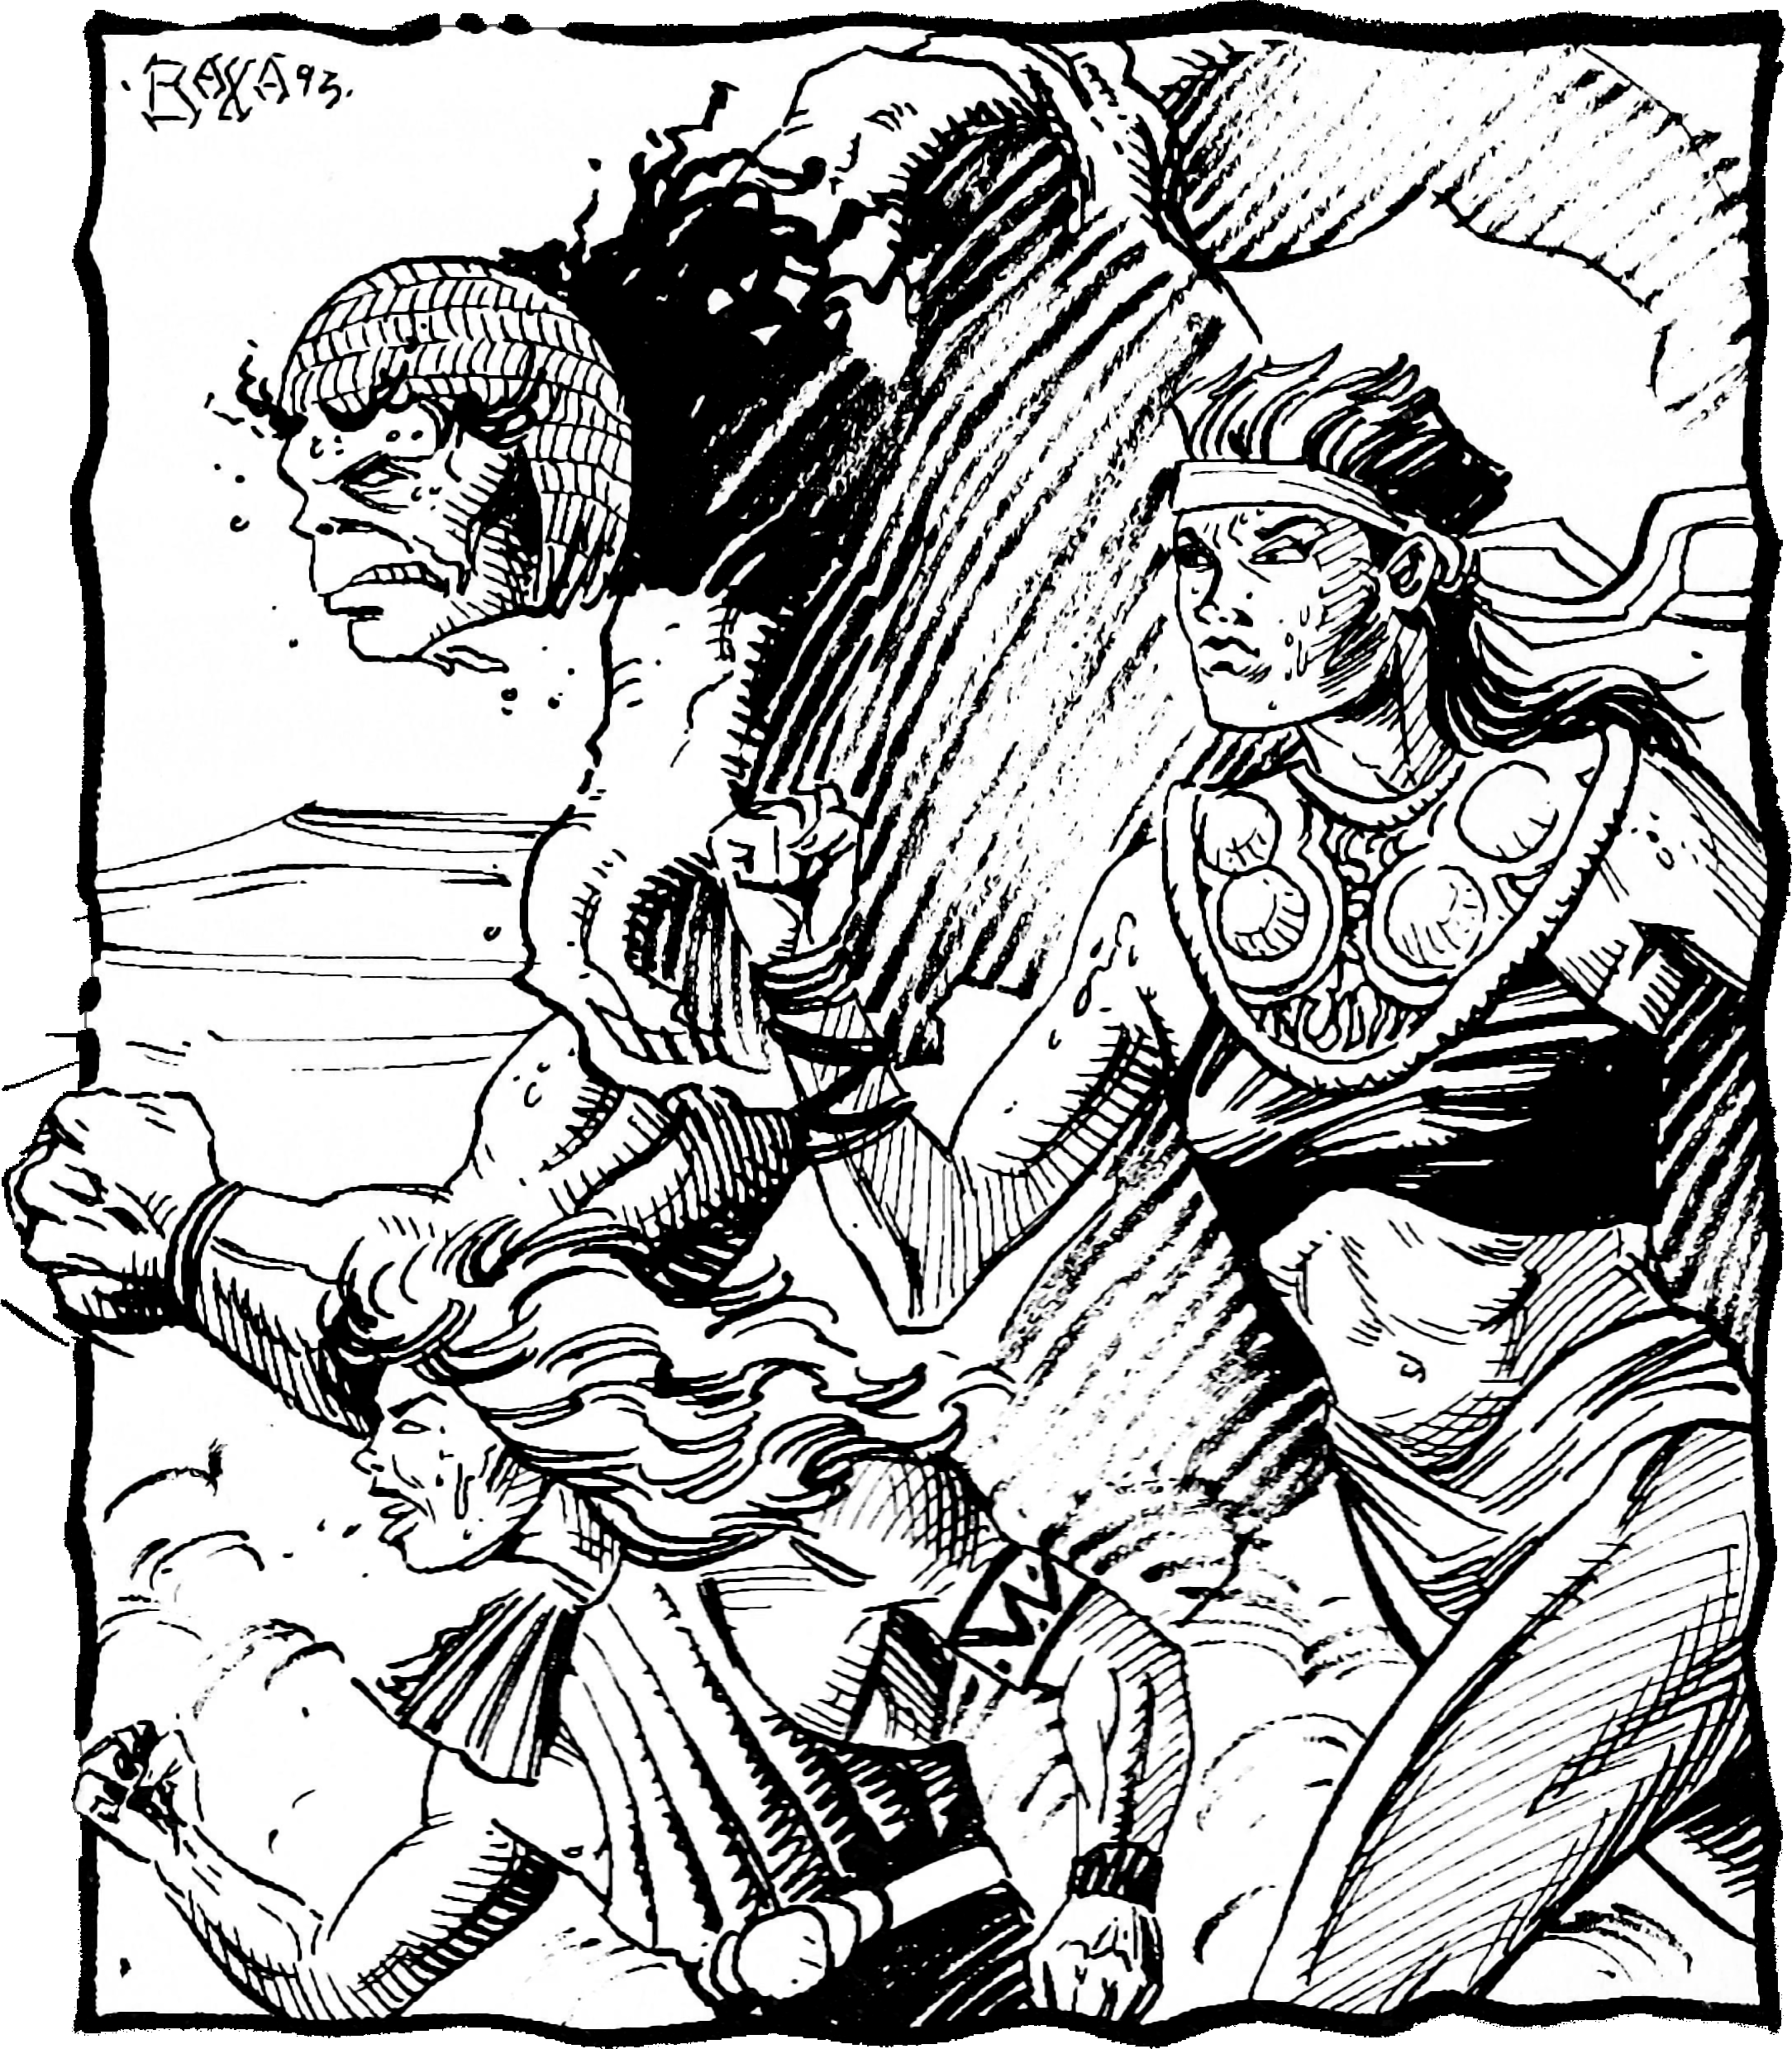
\includegraphics[width=\columnwidth]{images/running-1.png}
\WOTC
\end{figure}
\input{subsections/combat/actions-in-combat/full-round-actions/run.tex}

\subsubsection{Move 1.5 meter through Difficult Terrain}
In some situations, your movement may be so hampered that you don't have sufficient speed even to move 1.5 meter (a single square). In such a case, you may spend a full-round action to move 1.5 meter (1 square) in any direction, even diagonally. Even though this looks like a 1.5-meter step, it's not, and thus it provokes attacks of opportunity normally.
\subsection{Free Actions}
\Table{Free Actions}{LZ{14mm}}{
\tableheader Action & \tableheader Attack of Opportunity\footnotemark[1] \\
Cease concentration on a spell & No \\
Drop an item & No \\
Drop to the floor & No \\
Prepare spell components to cast a spell\footnotemark[2] & No \\
Speak & No \\
\TableNote{2}{1 Regardless of the action, if you move out of a threatened square, you usually provoke an attack of opportunity. This column indicates whether the action itself, not moving, provokes an attack of opportunity.}\\
\TableNote{2}{2 Unless the component is an extremely large or awkward item.}\\
}

Free actions don't take any time at all, though there may be limits to the number of free actions you can perform in a turn. Free actions rarely incur attacks of opportunity. Some common free actions are described below.

\subsubsection{Drop an Item}
Dropping an item in your space or into an adjacent square is a free action.

\subsubsection{Drop Prone}
Dropping to a prone position in your space is a free action.

\subsubsection{Speak}
In general, speaking is a free action that you can perform even when it isn't your turn. Speaking more than few sentences is generally beyond the limit of a free action.

\subsubsection{Cease Concentration on Spell}
You can stop concentrating on an active spell as a free action.

\Table{Swift Actions}{LZ{14mm}}{
\tableheader Action & \tableheader Attack of Opportunity\footnotemark[1] \\
Assume stance & No \\
Cast quickened spell & No \\
Cast spell (1 swift action casting time) & No \\
Use gladiatorial performance & No \\
Use quickened spell-like ability & No \\
\TableNote{2}{1 Regardless of the action, if you move out of a threatened square, you usually provoke an attack of opportunity. This column indicates whether the action itself, not moving, provokes an attack of opportunity.}\\
}

\subsection{Swift Actions}
A swift action consumes a very small amount of time, but represents a larger expenditure of effort and energy than a free action. You can perform one swift action per turn without affecting your ability to perform other actions. In that regard, a swift action is like a free action. However, you can perform only a single swift action per turn, regardless of what other actions you take. You can take a swift action any time you would normally be allowed to take a free action. Swift actions usually involve spellcasting or the activation of magic items; many characters (especially those who don't cast spells) never have an opportunity to take a swift action.

Casting a quickened spell is a swift action. In addition, casting any spell with a casting time of 1 swift action is a swift action.

Casting a spell with a casting time of 1 swift action does not provoke attacks of opportunity.

\subsection{Immediate Actions}
\Table{Immediate Actions}{LZ{14mm}}{
  \tableheader Action
& \tableheader Attack of Opportunity\footnotemark[1] \\
Cast spell (1 immediate action casting time) & No \\
Use the \feat{Greater Counterspell} feat     & Yes \\
Use martial prowess                          & No \\
\TableNote{2}{1 Regardless of the action, if you move out of a threatened square, you usually provoke an attack of opportunity. This column indicates whether the action itself, not moving, provokes an attack of opportunity.}\\
}

Much like a swift action, an immediate action consumes a very small amount of time, but represents a larger expenditure of effort and energy than a free action. However, unlike a swift action, an immediate action can be performed at any time---even if it's not your turn. An immediate action is an instant response to a trigger of some kind. For example, an attack, a spell cast, a successful hit, or enemy reaching a specific spot.

Casting \spell{feather fall} is an immediate action, since the spell can be cast at any time.

Using an immediate action on your turn is the same as using a swift action, and counts as your swift action for that turn. You cannot use another immediate action or a swift action until after your next turn if you have used an immediate action when it is not currently your turn (effectively, using an immediate action before your turn is equivalent to using your swift action for the coming turn). You also cannot use an immediate action if you are flat-footed.

\subsection{Miscellaneous Actions}
\Table{Miscellaneous Actions}{LZ{14mm}}{
  \tableheader No Action
& \tableheader Attack of Opportunity\footnotemark[1] \\
1.5-meter step                                    & No \\
Delay                                             & No \\
Fight defensively                                 & No \\
Make \skill{Concentration} check                  & No \\
Make passive \skill{Listen} or \skill{Spot} check & No \\

% \cmidrule[0pt]{1-2}

  \tableheader Action Type Varies
& \tableheader Attack of Opportunity\footnotemark[1] \\
Disarm\footnotemark[2]           & Yes \\
Grapple\footnotemark[2]          & Yes \\
Trip an opponent\footnotemark[2] & Yes \\
Use feat\footnotemark[3]         & Varies \\

\TableNote{2}{1 Regardless of the action, if you move out of a threatened square, you usually provoke an attack of opportunity. This column indicates whether the action itself, not moving, provokes an attack of opportunity.}\\
\TableNote{2}{2 These attack forms substitute for a melee attack, not an action. As melee attacks, they can be used once in an attack or charge action, one or more times in a full attack action, or even as an attack of opportunity.}\\
\TableNote{2}{3 The description of a feat defines its effect.}\\
}

\subsubsection{Take 1.5-Meter Step}
You can move 1.5 meter in any round when you don't perform any other kind of movement. Taking this 1.5-meter step never provokes an attack of opportunity. You can't take more than one 1.5-meter step in a round, and you can't take a 1.5-meter step in the same round when you move any distance.

You can take a 1.5-meter step before, during, or after your other actions in the round.

You can only take a 1.5-meter step if your movement isn't hampered by difficult terrain or darkness. Any creature with a speed of 1.5 meter or less can't take a 1.5-meter step, since moving even 1.5 meter requires a move action for such a slow creature.

You may not take a 1.5-meter step using a form of movement for which you do not have a listed speed.

\subsubsection{Use Feat}
Certain feats let you take special actions in combat. Other feats do not require actions themselves, but they give you a bonus when attempting something you can already do. Some feats are not meant to be used within the framework of combat. The individual feat descriptions tell you what you need to know about them.

\subsubsection{Use Skill}
Most skill uses are standard actions, but some might be move actions, full-round actions, free actions, or something else entirely.

The individual skill descriptions tell you what sorts of actions are required to perform skills.


\Figure*{b}{images/skeleton-1.png}
\section{Injury and Death}
Your hit points measure how hard you are to kill. No matter how many hit points you lose, your character isn't hindered in any way until your hit points drop to 0 or lower.

\subsection{Loss Of Hit Points}
The most common way that your character gets hurt is to take lethal damage and lose hit points.

\textbf{What Hit Points Represent:} Hit points mean two things in the game world: the ability to take physical punishment and keep going, and the ability to turn a serious blow into a less serious one.

\textbf{Effects of Hit Point Damage:} Damage doesn't slow you down until your current hit points reach 0 or lower. At 0 hit points, you're disabled.

At from $-1$ to $-9$ hit points, you're dying.

At $-10$ or lower, you're dead.

\textbf{Massive Damage:} If you ever sustain a single attack deals 50 points of damage or more and it doesn't kill you outright, you must make a DC 15 Fortitude save. If this saving throw fails, you die regardless of your current hit points. If you take 50 points of damage or more from multiple attacks, no one of which dealt 50 or more points of damage itself, the massive damage rule does not apply.

\subsection{Disabled (0 Hit Points)}
When your current hit points drop to exactly 0, you're disabled.

You can only take a single move or standard action each turn (but not both, nor can you take full$-round$ actions). You can take move actions without further injuring yourself, but if you perform any standard action (or any other strenuous action) you take 1 point of damage after the completing the act. Unless your activity increased your hit points, you are now at $-1$ hit points, and you're dying.

Healing that raises your hit points above 0 makes you fully functional again, just as if you'd never been reduced to 0 or fewer hit points.

You can also become disabled when recovering from dying. In this case, it's a step toward recovery, and you can have fewer than 0 hit points (see Stable Characters and Recovery, below).

\subsection{Dying ($-1$ to $-9$ Hit Points)}
When your character's current hit points drop to between $-1$ and $-9$ inclusive, he's dying.

A dying character immediately falls unconscious and can take no actions.

A dying character loses 1 hit point every round. This continues until the character dies or becomes stable (see below).

\subsection{Dead ($-10$ Hit Points or Lower)}
When your character's current hit points drop to $-10$ or lower, or if he takes massive damage (see above), he's dead. A character can also die from taking ability damage or suffering an ability drain that reduces his Constitution to 0.

\begin{figure*}[t!]
\centering
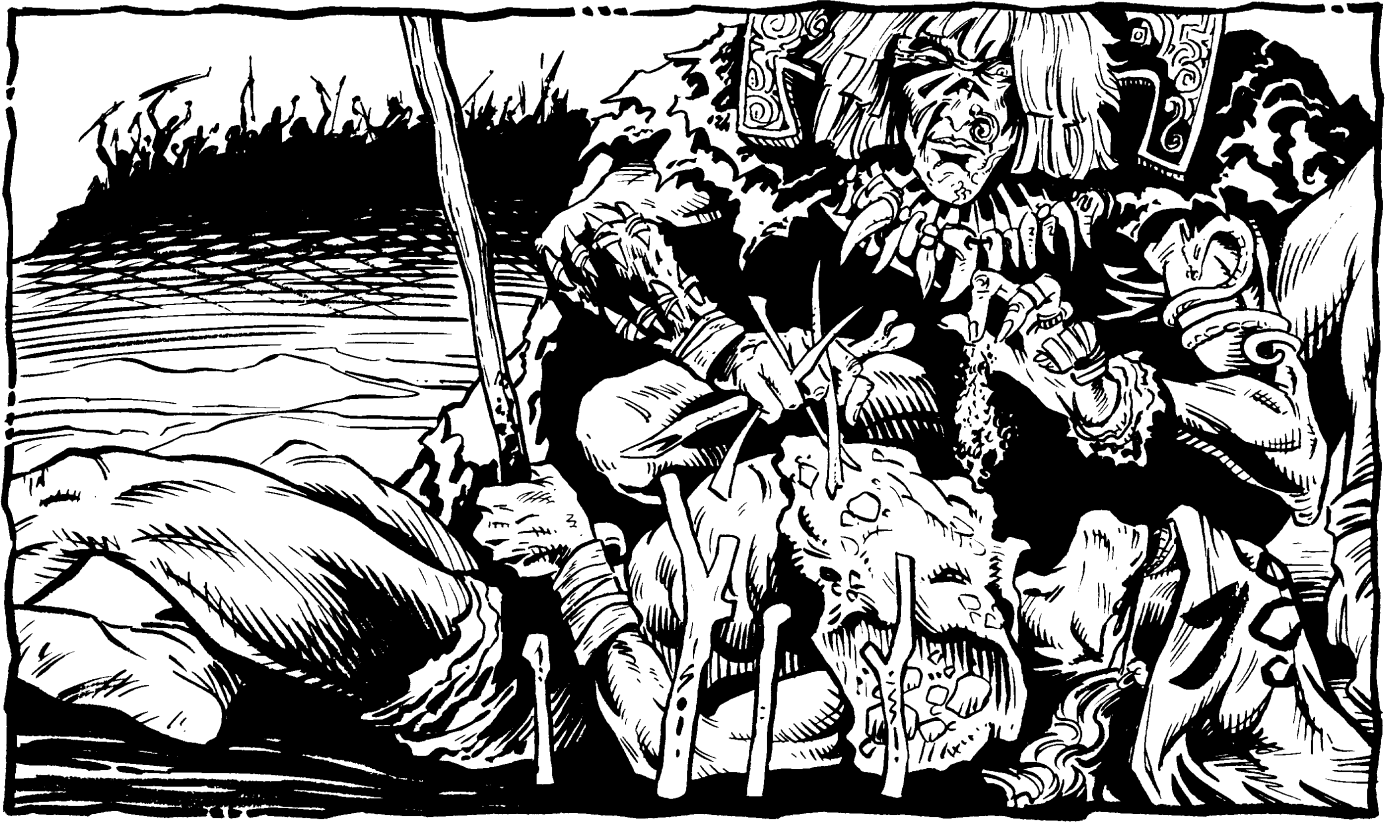
\includegraphics[width=\textwidth]{images/heal-1.png}
\WOTC
\end{figure*}
\subsection{Stable Characters and Recovery}
On the next turn after a character is reduced to between $-1$ and $-9$ hit points and on all subsequent turns, roll d\% to see whether the dying character becomes stable. He has a 10\% chance of becoming stable. If he doesn't, he loses 1 hit point. (A character who's unconscious or dying can't use any special action that changes the initiative count on which his action occurs.)

If the character's hit points drop to $-10$ or lower, he's dead.

You can keep a dying character from losing any more hit points and make him stable with a DC 15 \skill{Heal} check.

If any sort of healing cures the dying character of even 1 point of damage, he stops losing hit points and becomes stable.

Healing that raises the dying character's hit points to 0 makes him conscious and disabled. Healing that raises his hit points to 1 or more makes him fully functional again, just as if he'd never been reduced to 0 or lower. A spellcaster retains the spellcasting capability she had before dropping below 0 hit points.

A stable character who has been tended by a healer or who has been magically healed eventually regains consciousness and recovers hit points naturally. If the character has no one to tend him, however, his life is still in danger, and he may yet slip away.

\textbf{Recovering with Help:} One hour after a tended, dying character becomes stable, roll d\%. He has a 10\% chance of becoming conscious, at which point he is disabled (as if he had 0 hit points). If he remains unconscious, he has the same chance to revive and become disabled every hour. Even if unconscious, he recovers hit points naturally. He is back to normal when his hit points rise to 1 or higher.

\textbf{Recovering without Help:} A severely wounded character left alone usually dies. He has a small chance, however, of recovering on his own.

A character who becomes stable on his own (by making the 10\% roll while dying) and who has no one to tend to him still loses hit points, just at a slower rate. He has a 10\% chance each hour of becoming conscious. Each time he misses his hourly roll to become conscious, he loses 1 hit point. He also does not recover hit points through natural healing.

Even once he becomes conscious and is disabled, an unaided character still does not recover hit points naturally. Instead, each day he has a 10\% chance to start recovering hit points naturally (starting with that day); otherwise, he loses 1 hit point.

Once an unaided character starts recovering hit points naturally, he is no longer in danger of naturally losing hit points (even if his current hit point total is negative).

\subsection{Healing}
After taking damage, you can recover hit points through natural healing or through magical healing. In any case, you can't regain hit points past your full normal hit point total.

\textbf{Natural Healing:} With a full night's rest (8 hours of sleep or more), you recover 1 hit point per character level. Any significant interruption during your rest prevents you from healing that night.

If you undergo complete bed rest for an entire day and night, you recover twice your character level in hit points.

\textbf{Magical Healing:} Various abilities and spells can restore hit points.

\textbf{Healing Limits:} You can never recover more hit points than you lost. Magical healing won't raise your current hit points higher than your full normal hit point total.

\textbf{Healing Ability Damage:} Ability damage is temporary, just as hit point damage is. Ability damage returns at the rate of 1 point per night of rest (8 hours) for each affected ability score. Complete bed rest restores 2 points per day (24 hours) for each affected ability score.

\subsection{Temporary Hit Points}
Certain effects give a character temporary hit points. When a character gains temporary hit points, note his current hit point total. When the temporary hit points go away the character's hit points drop to his current hit point total. If the character's hit points are below his current hit point total at that time, all the temporary hit points have already been lost and the character's hit point total does not drop further.

When temporary hit points are lost, they cannot be restored as real hit points can be, even by magic.

\textbf{Increases in Constitution Score and Current Hit Points:} An increase in a character's Constitution score, even a temporary one, can give her more hit points (an effective hit point increase), but these are not temporary hit points. They can be restored and they are not lost first as temporary hit points are.

\subsection{Nonlethal Damage}
\textbf{Dealing Nonlethal Damage:} Certain attacks deal nonlethal damage. Other effects, such as heat or being exhausted, also deal nonlethal damage. When you take nonlethal damage, keep a running total of how much you've accumulated. Do not deduct the nonlethal damage number from your current hit points. It is not "real" damage. Instead, when your nonlethal damage equals your current hit points, you're staggered, and when it exceeds your current hit points, you fall unconscious. It doesn't matter whether the nonlethal damage equals or exceeds your current hit points because the nonlethal damage has gone up or because your current hit points have gone down.

\textit{Nonlethal Damage with a Weapon that Deals Lethal Damage:} You can use a melee weapon that deals lethal damage to deal nonlethal damage instead, but you take a $-4$ penalty on your attack roll.

\textit{Lethal Damage with a Weapon that Deals Nonlethal Damage:} You can use a weapon that deals nonlethal damage, including an unarmed strike, to deal lethal damage instead, but you take a $-4$ penalty on your attack roll.

\textbf{Staggered and Unconscious:} When your nonlethal damage equals your current hit points, you're staggered. You can only take a standard action or a move action in each round. You cease being staggered when your current hit points once again exceed your nonlethal damage.

When your nonlethal damage exceeds your current hit points, you fall unconscious. While unconscious, you are helpless.

Spellcasters who fall unconscious retain any spellcasting ability they had before going unconscious.

\textbf{Healing Nonlethal Damage:} You heal nonlethal damage at the rate of 1 hit point per hour per character level.

When a spell or a magical power cures hit point damage, it also removes an equal amount of nonlethal damage.


\section{Movement and Distance}
% \section{Movement, Position, and Distance}
Miniatures are on the 30mm scale---a miniature figure of a 1.8-meter-tall human is approximately 30mm tall. A square on the battle grid is 2.5 centimeters across, representing a 1.5-meter-by-1.5-meter area.

\subsection{Tactical Movement}
The characteristics of moving in a combat situation: distance to be covered, the possible impediments, and special rules are described below.


\Figure*{t}{images/kirre.png}

\input{subsections/combat/movement-position-and-distance/tactical-movement/how-far-can-your-character-move.tex}

\subsubsection{Measuring Distance}
\textbf{Diagonals:} When measuring distance, the first diagonal counts as 1 square, the second counts as 2 squares, the third counts as 1, the fourth as 2, and so on.

You can't move diagonally past a corner (even by taking a 1.5-meter step). You can move diagonally past a creature, even an opponent.

You can also move diagonally past other impassable obstacles, such as pits.

\textbf{Closest Creature:} When it's important to determine the closest square or creature to a location, if two squares or creatures are equally close, randomly determine which one counts as closest by rolling a die.

\input{subsections/combat/movement-position-and-distance/tactical-movement/moving-through-a-square.tex}
\input{subsections/combat/movement-position-and-distance/tactical-movement/terrain-and-obstacles.tex}

\BigTableBottom{Creature Size and Scale}{l*{3}{Z{12mm}}XX*{3}{Z{14mm}}}{
\tableheader Size Category &
\tableheader Size\footnotemark[1] Modifier &
\tableheader Grapple\footnotemark[2] Modifier &
\tableheader Hide\footnotemark[3] Modifier &
\tableheader Height or Length\footnotemark[4] &
\tableheader Weight\footnotemark[5] &
\tableheader Space\footnotemark[6] &
\tableheader Natural Reach\footnotemark[6] (Tall) &
\tableheader Natural Reach\footnotemark[6] (Long)\\

Fine       & +8   & $-16$ & +16   & 15 cm or less  & 60 g or less        & 15 cm & 0 m   & 0 m   \\
Diminutive & +4   & $-12$ & +12   & 15 cm--30 cm   & 60 g--0.5 kg        & 30 cm & 0 m   & 0 m   \\
Tiny       & +2   & $-8$  & +8    & 30 cm--60 cm   & 0.5 kg--4 kg        & 75 cm & 0 m   & 0 m   \\
Small      & +1   & $-4$  & +4    & 60 cm--1.2 m   & 4 kg--30 kg         & 1.5 m & 1.5 m & 1.5 m \\
Medium     & +0   & +0    & +0    & 1.2 m--2.5 m   & 30 kg--250 kg       & 1.5 m & 1.5 m & 1.5 m \\
Large      & $-1$ & +4    & $-4$  & 2.5 m--5 m   & 250 kg--1 tonne     & 3 m   & 3 m   & 1.5 m \\
Huge       & $-2$ & +8    & $-8$  & 5 m--10 m   & 1 tonne--8 tonnes   & 4.5 m & 4.5 m & 3 m   \\
Gargantuan & $-4$ & +12   & $-12$ & 10 m--20 m  & 8 tonnes--60 tonnes & 6 m   & 6 m   & 4.5 m \\
Colossal   & $-8$ & +16   & $-16$ & 20 m or more & 60 tonnes or more   & 9 m   & 9 m   & 6 m   \\

\BigTableNote{9}{1 A creature's size modifier is applied to it's attack bonus and Armor Class.}\\
\BigTableNote{9}{2 See the Grapple special attack.}\\
\BigTableNote{9}{3 See the \skill{Hide} skill.}\\
\BigTableNote{9}{4 Biped's height, quadruped's body length (nose to base of tail)}\\
\BigTableNote{9}{5 Assumes that the creature is roughly as dense as a regular animal. A creature made of stone will weigh considerably more. A gaseous creature will weigh much less.}\\
\BigTableNote{9}{6 These values are typical for creatures of the indicated size. Some exceptions exist.}\\
}
\input{subsections/combat/movement-position-and-distance/tactical-movement/special-movement-rules.tex}

% \Figure*[\textwidth-22mm]{t}{images/sizes-1.png}

\subsection{Big and Little Creatures}
% \subsection{Big and Little Creatures In Combat}
Creatures smaller than Small or larger than Medium have special rules relating to position, reach, and weapon size.

\textbf{Tiny, Diminutive, and Fine Creatures:} Very small creatures take up less than 1 square of space. This means that more than one such creature can fit into a single square. A Tiny creature typically occupies a space only 75 centimeters across, so four can fit into a single square. Twenty-five Diminutive creatures or 100 Fine creatures can fit into a single square.

Creatures that take up less than 1 square of space typically have a natural reach of 0 meters, meaning they can't reach into adjacent squares. They must enter an opponent's square to attack in melee. This provokes an attack of opportunity from the opponent. You can attack into your own square if you need to, so you can attack such creatures normally.

Since they have no natural reach, they do not threaten the squares around them. You can move past them without provoking attacks of opportunity. They also can't flank an enemy.

\Figure{b}{images/sizes-1.png}
\textbf{Large, Huge, Gargantuan, and Colossal Creatures:} Very large creatures take up more than 1 square. For instance, a half-giant takes up a space 3 meters on a side (2 squares wide).

Creatures that take up more than 1 square typically have a natural reach of 3 meters or more, meaning that they can reach targets even if they aren't in adjacent squares.

Unlike when someone uses a reach weapon, a creature with greater than normal natural reach (more than 1.5 meter) still threatens squares adjacent to it. A creature with greater than normal natural reach usually gets an attack of opportunity against you if you approach it, because you must enter and move within the range of its reach before you can attack it. (This attack of opportunity is not provoked if you take a 1.5-meter step.)

Large or larger creatures using reach weapons can strike up to double their natural reach but can't strike at their natural reach or less.

\section{Combat Modifiers}
Sometimes you just have to go toe-to-toe in a fight, but you can usually gain some advantage by seeking a better position, either offensively or defensively. This section covers the rules for when you can line up a particularly good attack or are forced to make a disadvantageous one.

\subsection{(Un)Favorable Conditions}
% \subsection{Favorable and Unfavorable Conditions}
Depending on the condition of attackers or defenders, they may gain bonuses or penalties as stated in \tabref{Attack Roll Modifiers} and \tabref{Armor Class Modifiers}.

\Table{Attack Roll Modifiers}{Xcc}{
\tableheader Attacker is... & \tableheader Melee & \tableheader Ranged\\
Dazzled                   & $-1$                 & $-1$ \\
Entangled                 & $-2$\footnotemark[1] & $-2$\footnotemark[1] \\
Flanking defender         & Advantage            & --- \\
Invisible                 & +2\footnotemark[2]   & +2\footnotemark[2] \\
On higher ground          & +1                   & +0 \\
Prone                     & Disadvantage         & ---\footnotemark[3] \\
Shaken or frightened      & $-2$                 & $-2$ \\
Squeezing through a space & Disadvantage         & Disadvantage \\

\TableNote{3}{1 An entangled character also takes a $-4$ penalty to Dexterity, which may affect his attack roll.}\\
\TableNote{3}{2 The defender loses any Dexterity bonus to AC. This bonus doesn't apply if the target is blinded.}\\
\TableNote{3}{3 Most ranged weapons can't be used while the attacker is prone, but you can use a crossbow or shuriken while prone at no penalty.}\\
}

\Table{Armor Class Modifiers}{L*{2}{Z{12mm}}}{
\tableheader Defender is... & \tableheader Melee & \tableheader Ranged\\
Behind cover & +4 & +4 \\
Blinded & $-2$\footnotemark[1] & $-2$\footnotemark[1] \\
Concealed or invisible & \multicolumn{2}{c}{See Concealment} \\
Cowering & $-2$\footnotemark[1] & $-2$\footnotemark[1] \\
Entangled & +0\footnotemark[2] & +0\footnotemark[2] \\
Flat-footed (such as surprised, balancing, climbing) & +0\footnotemark[1] & +0\footnotemark[1] \\
Grappling (but attacker is not) & +0\footnotemark[1] & +0\footnotemark[1]\footnotemark[3] \\
Helpless (such as paralyzed, sleeping, or bound) & $-4$\footnotemark[4] & +0\footnotemark[4] \\
Kneeling or sitting & $-2$ & +2 \\
Pinned & $-4$\footnotemark[4] & +0\footnotemark[4] \\
Prone & $-4$ & +4 \\
Squeezing through a space & $-4$ & $-4$ \\
Stunned & -2\footnotemark[1] & -2\footnotemark[1] \\

\TableNote{3}{1 The defender loses any Dexterity bonus to AC.}\\
\TableNote{3}{2 An entangled character takes a $-4$ penalty to Dexterity.}\\
\TableNote{3}{3 Roll randomly to see which grappling combatant you strike. That defender loses any Dexterity bonus to AC.}\\
\TableNote{3}{4 Treat the defender's Dexterity as 0 ($-5$ modifier). Rogues can sneak attack helpless or pinned defenders.}\\
}

\begin{figure*}[t!]
\centering
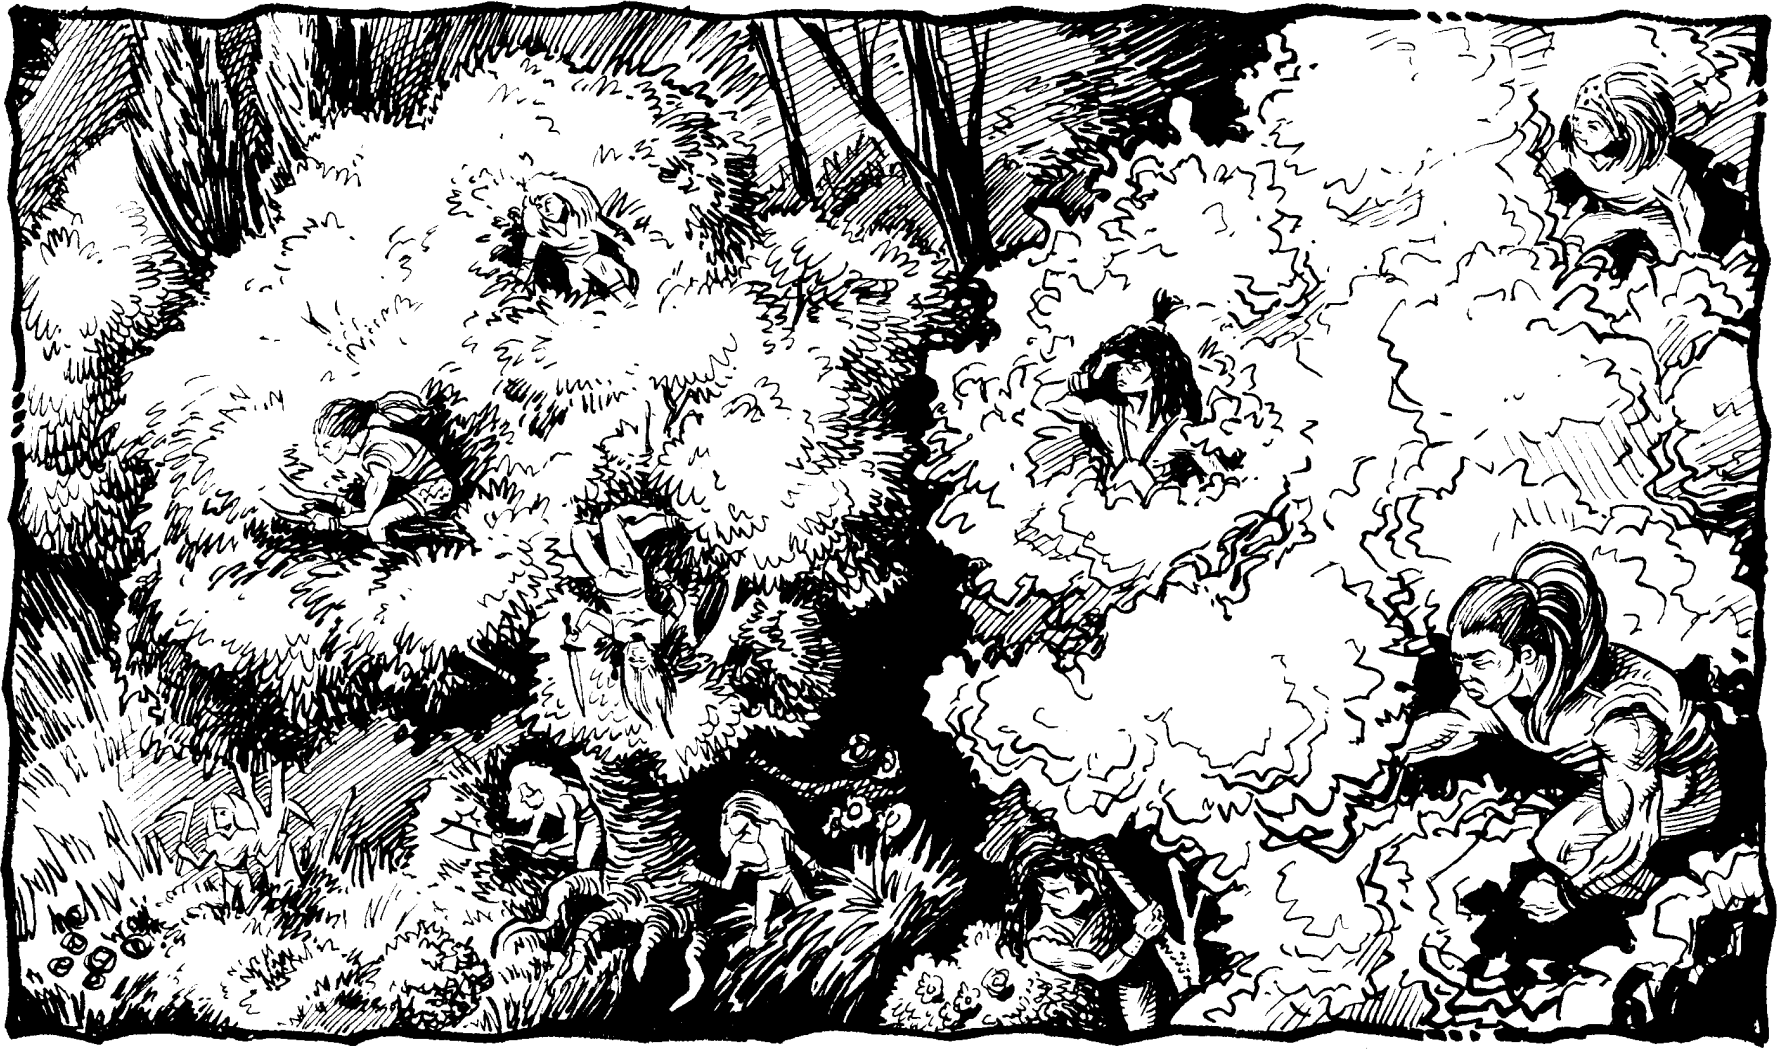
\includegraphics[width=\textwidth]{images/cover-1.png}
\WOTC
\end{figure*}
\subsection{Cover}
To determine whether your target has cover from your ranged attack, choose a corner of your square. If any line from this corner to any corner of the target's square passes through a square or border that blocks line of effect or provides cover, or through a square occupied by a creature, the target has cover (+4 to AC).

When making a melee attack against an adjacent target, your target has cover if any line from your square to the target's square goes through a wall (including a low wall). When making a melee attack against a target that isn't adjacent to you (such as with a reach weapon), use the rules for determining cover from ranged attacks.

\textbf{Low Obstacles and Cover:} A low obstacle (such as a wall no higher than half your height) provides cover, but only to creatures within 9 meters (6 squares) of it. The attacker can ignore the cover if he's closer to the obstacle than his target.

\textbf{Cover and Attacks of Opportunity:} You can't execute an attack of opportunity against an opponent with cover relative to you.

\textbf{Cover and Reflex Saves:} Cover grants you a +2 bonus on Reflex saves against attacks that originate or burst out from a point on the other side of the cover from you. Note that spread effects can extend around corners and thus negate this cover bonus.

\textbf{Cover and Hide Checks:} You can use cover to make a \skill{Hide} check. Without cover, you usually need concealment to make a \skill{Hide} check.

\textbf{Soft Cover:} Creatures, even your enemies, can provide you with cover against ranged attacks, giving you a +4 bonus to AC. However, such soft cover provides no bonus on Reflex saves, nor does soft cover allow you to make a \skill{Hide} check.

\textbf{Big Creatures and Cover:} Any creature with a space larger than 1.5 meter (1 square) determines cover against melee attacks slightly differently than smaller creatures do. Such a creature can choose any square that it occupies to determine if an opponent has cover against its melee attacks. Similarly, when making a melee attack against such a creature, you can pick any of the squares it occupies to determine if it has cover against you.

\textbf{Total Cover:} If you don't have line of effect to your target he is considered to have total cover from you. You can't make an attack against a target that has total cover.

\textbf{Varying Degrees of Cover:} In some cases, cover may provide a greater bonus to AC and Reflex saves. In such situations the normal cover bonuses to AC and Reflex saves can be doubled (to +8 and +4, respectively). A creature with this improved cover effectively gains improved evasion against any attack to which the Reflex save bonus applies. Furthermore, improved cover provides a +10 bonus on \skill{Hide} checks.
\subsection{Concealment}
To determine whether your target has concealment from your ranged attack, choose a corner of your square. If any line from this corner to any corner of the target's square passes through a square or border that provides concealment, the target has concealment.

When making a melee attack against an adjacent target, your target has concealment if his space is entirely within an effect that grants concealment. When making a melee attack against a target that isn't adjacent to you use the rules for determining concealment from ranged attacks.

In addition, some magical effects provide concealment against all attacks, regardless of whether any intervening concealment exists.

\textbf{Concealment Miss Chance:} Concealment gives the subject of a successful attack a 20\% chance that the attacker missed because of the concealment. If the attacker hits, the defender must make a miss chance percentile roll to avoid being struck. Multiple concealment conditions do not stack.

\textbf{Concealment and Hide Checks:} You can use concealment to make a Hide check. Without concealment, you usually need cover to make a Hide check.

\textbf{Total Concealment:} If you have line of effect to a target but not line of sight he is considered to have total concealment from you. You can't attack an opponent that has total concealment, though you can attack into a square that you think he occupies. A successful attack into a square occupied by an enemy with total concealment has a 50\% miss chance (instead of the normal 20\% miss chance for an opponent with concealment).

You can't execute an attack of opportunity against an opponent with total concealment, even if you know what square or squares the opponent occupies.

\textbf{Ignoring Concealment:} Concealment isn't always effective. A shadowy area or darkness doesn't provide any concealment against an opponent with darkvision. Characters with low-light vision can see clearly for a greater distance with the same light source than other characters. Although invisibility provides total concealment, sighted opponents may still make Spot checks to notice the location of an invisible character. An invisible character gains a +20 bonus on Hide checks if moving, or a +40 bonus on Hide checks when not moving (even though opponents can't see you, they might be able to figure out where you are from other visual clues).

\textbf{Varying Degrees of Concealment:} Certain situations may provide more or less than typical concealment, and modify the miss chance accordingly.
\subsection{Flanking}
When making a melee attack, you get a +2 flanking bonus if your opponent is threatened by a character or creature friendly to you on the opponent's opposite border or opposite corner.

When in doubt about whether two friendly characters flank an opponent in the middle, trace an imaginary line between the two friendly characters' centers. If the line passes through opposite borders of the opponent's space (including corners of those borders), then the opponent is flanked.

\textit{Exception:} If a flanker takes up more than 1 square, it gets the flanking bonus if any square it occupies counts for flanking.

Only a creature or character that threatens the defender can help an attacker get a flanking bonus.

Creatures with a reach of 0 feet can't flank an opponent.
\subsection{Helpless Defenders}
A helpless opponent is someone who is bound, sleeping, paralyzed, unconscious, or otherwise at your mercy.

\textbf{Regular Attack:} A helpless character takes a $-4$ penalty to AC against melee attacks, but no penalty to AC against ranged attacks.

A helpless defender can't use any Dexterity bonus to AC. In fact, his Dexterity score is treated as if it were 0 and his Dexterity modifier to AC as if it were $-5$ (and a rogue can sneak attack him).

\textbf{Coup de Grace:} As a full-round action, you can use a melee weapon to deliver a coup de grace to a helpless opponent. You can also use a bow or crossbow, provided you are adjacent to the target.

You automatically hit and score a critical hit. If the defender survives the damage, he must make a Fortitude save (DC 10 + damage dealt) or die. A rogue also gets her extra sneak attack damage against a helpless opponent when delivering a coup de grace.

Delivering a coup de grace provokes attacks of opportunity from threatening opponents.

You can't deliver a coup de grace against a creature that is immune to critical hits. You can deliver a coup de grace against a creature with total concealment, but doing this requires two consecutive full-round actions (one to ``find'' the creature once you've determined what square it's in, and one to deliver the coup de grace).

\subsection{Proficiencies}
A character who uses a weapon with which they are not proficient gets disadvantage on attack rolls.

A character who wears armor and/or uses a shield with which they are not proficient takes the armor's (and/or shield's) armor check penalty on attack rolls and on all Strength-based and Dexterity-based ability and skill checks. The penalty for nonproficiency with armor stacks with the penalty for nonproficiency with shields

Weapon, armor, or shield proficiency may be granted by the character's race, class or by the following feats:

\begin{itemize*}
\item \feat{Armor Proficiency (Light)}
\item \feat{Armor Proficiency (Medium)}
\item \feat{Armor Proficiency (Heavy)}
\item \feat{Exotic Weapon Proficiency}
\item \feat{Martial Weapon Proficiency}
\item \feat{Shield Proficiency}
\item \feat{Simple Weapon Proficiency}
\item \feat{Tower Shield Proficiency}
\end{itemize*}

\section{Special Attacks}
This section covers grappling, feinting, mounted combats, and all other forms of special attacks.

\Table{Special Attacks}{lX}{
\tableheader Special Attack & \tableheader Brief Description\\
Aid another         & Grant an ally advantage on attacks or give disadvantage on an enemy's\\
Bull rush           & Push an opponent back 1.5 meter or more\\
Charge              & Move up to twice your speed and attack with a +2 bonus\\
Disarm              & Knock a weapon from your opponent's hands, or grab a worn item\\
Feint               & Negate your opponent's Dex bonus to AC\\
Grapple             & Wrestle with an opponent\\
Mounted Combat      & Fight while riding your steed\\
Overrun             & Plow past or over an opponent as you move\\
Sunder              & Strike an opponent's weapon or shield\\
Throw splash weapon & Throw container of dangerous liquid at target\\
Trip                & Trip an opponent\\
Turn/rebuke undead  & Channel positive (or negative) energy to turn away (or awe) undead\\
Two-weapon fighting & Fight with a weapon in each hand\\
}
\subsection{Aid Another}
In melee combat, you can help a friend attack or defend by distracting or interfering with an opponent. If you're in position to make a melee attack on an opponent that is engaging a friend in melee combat, you can attempt to aid your friend as a standard action. You make an attack roll against AC 10. If you succeed, your friend gains either gains advantage on his next attack roll against that opponent or that opponent has disadvantage on their next attack against your friend (your choice), as long as that attack comes before the beginning of your next turn. Multiple characters can aid the same friend, and similar bonuses stack.

You can also use this standard action to help a friend in other ways, such as when he is affected by a spell, or to assist another character's skill check.
\subsection{Bull Rush}
You can make a bull rush as a standard action (an attack) or as part of a charge. When you make a bull rush, you attempt to push an opponent straight back instead of damaging him. You can only bull rush an opponent who is one size category larger than you, the same size, or smaller.

\textbf{Initiating a Bull Rush:} First, you move into the defender's space. Doing this provokes an attack of opportunity from each opponent that threatens you, including the defender. (If you have the \feat{Improved Bull Rush} feat, you don't provoke an attack of opportunity from the defender.) Any attack of opportunity made by anyone other than the defender against you during a bull rush has a 25\% chance of accidentally targeting the defender instead, and any attack of opportunity by anyone other than you against the defender likewise has a 25\% chance of accidentally targeting you. (When someone makes an attack of opportunity, make the attack roll and then roll to see whether the attack went astray.)

Second, you and the defender make opposed Strength checks. You each add a +4 bonus for each size category you are larger than Medium or a $-4$ penalty for each size category you are smaller than Medium. You get advantage on your check if you are charging. The defender gets advantage on his roll if he has more than two legs or is otherwise exceptionally stable.

\textbf{Bull Rush Results:} If you beat the defender's Strength check result, you push him back 1.5 meter. If you wish to move with the defender, you can push him back an additional 1.5 meter for each 5 points by which your check result is greater than the defender's check result. You can't, however, exceed your normal movement limit. (Note: The defender provokes attacks of opportunity if he is moved. So do you, if you move with him. The two of you do not provoke attacks of opportunity from each other, however.)

If you fail to beat the defender's Strength check result, you move 1.5 meter straight back to where you were before you moved into his space. If that space is occupied, you fall prone in that space.
\Figure{b}{images/riders.png}
\subsection{Charge}
Charging is a special full-round action that allows you to move up to twice your speed and attack during the action. However, it carries tight restrictions on how you can move.

\textbf{Movement During a Charge:} You must move before your attack, not after. You must move at least 3 meters (2 squares) and may move up to double your speed directly toward the designated opponent.

You must have a clear path toward the opponent, and nothing can hinder your movement (such as difficult terrain or obstacles). Here's what it means to have a clear path. First, you must move to the closest space from which you can attack the opponent. (If this space is occupied or otherwise blocked, you can't charge.) Second, if any line from your starting space to the ending space passes through a square that blocks movement, slows movement, or contains a creature (even an ally), you can't charge. (Helpless creatures don't stop a charge.)

If you don't have line of sight to the opponent at the start of your turn, you can't charge that opponent.

You can't take a 1.5-meter step in the same round as a charge.

If you are able to take only a standard action or a move action on your turn, you can still charge, but you are only allowed to move up to your speed (instead of up to double your speed). You can't use this option unless you are restricted to taking only a standard action or move action on your turn.

\textbf{Attacking on a Charge:} After moving, you may make a single melee attack. You get a +2 bonus on the attack roll and take a $-2$ penalty to your AC until the start of your next turn.

A charging character gets advantage on the Strength check made to bull rush an opponent.

Even if you have extra attacks, such as from having a high enough base attack bonus or from using multiple weapons, you only get to make one attack during a charge.

\textbf{Lances and Charge Attacks:} A lance deals double damage if employed by a mounted character in a charge.

\textbf{Weapons Readied against a Charge:} Spears, tridents, and certain other piercing weapons deal double damage when readied (set) and used against a charging character.
\subsection{Disarm}
As a melee attack, you may attempt to disarm your opponent. If you do so with a weapon, you knock the opponent's weapon out of his hands and to the ground. If you attempt the disarm while unarmed, you end up with the weapon in your hand.

If you're attempting to disarm a melee weapon, follow the steps outlined here. If the item you are attempting to disarm isn't a melee weapon the defender may still oppose you with an attack roll, but takes a penalty and can't attempt to disarm you in return if your attempt fails.

\begin{enumerate*}
\item \textbf{Attack of Opportunity.} You provoke an attack of opportunity from the target you are trying to disarm. (If you have the \feat{Improved Disarm} feat, you don't incur an attack of opportunity for making a disarm attempt.) If the defender's attack of opportunity deals any damage, your disarm attempt fails.

\item \textbf{Opposed Rolls.} You and the defender make opposed attack rolls with your respective weapons. The wielder of a two-handed weapon on a disarm attempt gets advantage on this roll, and the wielder of a light weapon get disadvantage on the roll. (An unarmed strike is considered a light weapon, so you always get disadvantage when trying to disarm an opponent by using an unarmed strike.) If the combatants are of different sizes, the larger combatant gets a bonus on the attack roll of +4 per difference in size category. If the targeted item isn't a melee weapon, the defender gets disadvantage on the roll.

\item \textbf{Consequences.} If you beat the defender, the defender is disarmed. If you attempted the disarm action unarmed, you now have the weapon. If you were armed, the defender's weapon is on the ground in the defender's square.
\end{enumerate*}

If you fail on the disarm attempt, the defender may immediately react and attempt to disarm you with the same sort of opposed melee attack roll. His attempt does not provoke an attack of opportunity from you. If he fails his disarm attempt, you do not subsequently get a free disarm attempt against him.

\textit{Note:} A defender wearing spiked gauntlets can't be disarmed. A defender using a weapon attached to a locked gauntlet gets a +10 bonus to resist being disarmed.

\subsubsection{Grabbing Items}
You can use a disarm action to snatch an item worn by the target. If you want to have the item in your hand, the disarm must be made as an unarmed attack.

If the item is poorly secured or otherwise easy to snatch or cut away the attacker gets a +4 bonus. Unlike on a normal disarm attempt, failing the attempt doesn't allow the defender to attempt to disarm you. This otherwise functions identically to a disarm attempt, as noted above.

You can't snatch an item that is well secured unless you have pinned the wearer (see Grapple). Even then, the defender gains a +4 bonus on his roll to resist the attempt.
\subsection{Feint}
Feinting is a standard action. To feint, make a \skill{Bluff} check opposed by a \skill{Sense Motive} check by your target. The target may add his base attack bonus to this \skill{Sense Motive} check. If your \skill{Bluff} check result exceeds your target's \skill{Sense Motive} check result, the next melee attack you make against the target does not allow him to use his Dexterity bonus to AC (if any). This attack must be made on or before your next turn.

When feinting in this way against a creature of a different shape than yours, you get disadvantage on your roll. For example, an elf would get disadvantage on her \skill{Bluff} check to feint a thri-kreen, since she is humanoid and he is a insectoid. At the same time, he would roll with disadvantage if he tries to feint the elf.

Against a creature of animal Intelligence (1 or 2), you take a $-8$ penalty. Against a nonintelligent creature, it's impossible.

Feinting in combat does not provoke attacks of opportunity.

\textbf{Feinting as a Move Action:} With the \feat{Improved Feint} feat, you can attempt a feint as a move action instead of as a standard action.
\Figure*{t}{images/behir.png}
\subsection{Grapple}
Grappling is holding an opponent in hand-to-hand combat, very common in smaller gladiatorial arenas. For monsters, it can mean locking you in its mouth, or holding you down in the ground.

\subsubsection{Grapple Checks}
Repeatedly in a grapple, you need to make opposed grapple checks against an opponent. A grapple check is like a melee attack roll. Your attack bonus on a grapple check is:

{
	\centering
	\vskip1em
	\Large \textit{Base attack bonus} + \textit{Str. modifier}\\ + \textit{special size modifier}
	\vskip1em
}

\textbf{Special Size Modifier:} The special size modifier for a grapple check is as follows: Colossal +16, Gargantuan +12, Huge +8, Large +4, Medium +0, Small $-4$, Tiny $-8$, Diminutive $-12$, Fine $-16$. Use this number in place of the normal size modifier you use when making an attack roll.

\subsubsection{Starting a Grapple}
To start a grapple, you need to grab and hold your target. Starting a grapple requires a successful melee attack roll. If you get multiple attacks, you can attempt to start a grapple multiple times (at successively lower base attack bonuses).

\begin{enumerate*}
\item \textbf{Attack of Opportunity.} You provoke an attack of opportunity from the target you are trying to grapple. If the attack of opportunity deals damage, the grapple attempt fails. (Certain monsters do not provoke attacks of opportunity when they attempt to grapple, nor do characters with the Improved Grapple feat.) If the attack of opportunity misses or fails to deal damage, proceed to Step 2.

\item \textbf{Grab.} You make a melee touch attack to grab the target. If you fail to hit the target, the grapple attempt fails. If you succeed, proceed to Step 3.

\item \textbf{Hold.} Make an opposed grapple check as a free action. If you succeed, you and your target are now grappling, and you deal damage to the target as if with an unarmed strike.

If you lose, you fail to start the grapple. You automatically lose an attempt to hold if the target is two or more size categories larger than you are.

In case of a tie, the combatant with the higher grapple check modifier wins. If this is a tie, roll again to break the tie.

\item \textbf{Maintain Grapple.} To maintain the grapple for later rounds, you must move into the target's space. (This movement is free and doesn't count as part of your movement in the round.) Moving, as normal, provokes attacks of opportunity from threatening opponents, but not from your target.

If you can't move into your target's space, you can't maintain the grapple and must immediately let go of the target. To grapple again, you must begin at Step 1.
\end{enumerate*}

\subsubsection{Grappling Consequences}
While you're grappling, your ability to attack others and defend yourself is limited.

\textbf{No Threatened Squares:} You don't threaten any squares while grappling.

\textbf{No Dexterity Bonus:} You lose your Dexterity bonus to AC (if you have one) against opponents you aren't grappling. (You can still use it against opponents you are grappling.)

\textbf{No Movement:} You can't move normally while grappling. You may, however, make an opposed grapple check to move while grappling.

\subsubsection{If You're Grappling}
When you are grappling (regardless of who started the grapple), you can perform any of the following actions. Some of these actions take the place of an attack (rather than being a standard action or a move action). If your base attack bonus allows you multiple attacks, you can attempt one of these actions in place of each of your attacks, but at successively lower base attack bonuses.

\textbf{Activate a Magic Item:} You can activate a magic item, as long as the item doesn't require spell completion activation. You don't need to make a grapple check to activate the item.

\textbf{Attack Your Opponent:} You can make an attack with an unarmed strike, natural weapon, or light weapon against another character you are grappling. You take a $-4$ penalty on such attacks.

You can't attack with two weapons while grappling, even if both are light weapons.

\textbf{Cast a Spell:} You can attempt to cast a spell while grappling or even while pinned (see below), provided its casting time is no more than 1 standard action, it has no somatic component, and you have in hand any material components or focuses you might need. Any spell that requires precise and careful action is impossible to cast while grappling or being pinned. If the spell is one that you can cast while grappling, you must make a Concentration check (DC 20 + spell level) or lose the spell. You don't have to make a successful grapple check to cast the spell.

\textbf{Damage Your Opponent:} While grappling, you can deal damage to your opponent equivalent to an unarmed strike. Make an opposed grapple check in place of an attack. If you win, you deal nonlethal damage as normal for your unarmed strike (1d3 points for Medium attackers or 1d2 points for Small attackers, plus Strength modifiers). If you want to deal lethal damage, you take a $-4$ penalty on your grapple check.

\textit{Exception:} Monks deal more damage on an unarmed strike than other characters, and the damage is lethal. However, they can choose to deal their damage as nonlethal damage when grappling without taking the usual $-4$ penalty for changing lethal damage to nonlethal damage.

\textbf{Draw a Light Weapon:} You can draw a light weapon as a move action with a successful grapple check.

\textbf{Escape from Grapple:} You can escape a grapple by winning an opposed grapple check in place of making an attack. You can make an Escape Artist check in place of your grapple check if you so desire, but this requires a standard action. If more than one opponent is grappling you, your grapple check result has to beat all their individual check results to escape. (Opponents don't have to try to hold you if they don't want to.) If you escape, you finish the action by moving into any space adjacent to your opponent(s).

\textbf{Move:} You can move half your speed (bringing all others engaged in the grapple with you) by winning an opposed grapple check. This requires a standard action, and you must beat all the other individual check results to move the grapple.

\textit{Note:} You get a +4 bonus on your grapple check to move a pinned opponent, but only if no one else is involved in the grapple.

\textbf{Retrieve a Spell Component:} You can produce a spell component from your pouch while grappling by using a full-round action. Doing so does not require a successful grapple check.

\textbf{Pin Your Opponent:} You can hold your opponent immobile for 1 round by winning an opposed grapple check (made in place of an attack). Once you have an opponent pinned, you have a few options available to you (see below).

\textbf{Break Another's Pin:} If you are grappling an opponent who has another character pinned, you can make an opposed grapple check in place of an attack. If you win, you break the hold that the opponent has over the other character. The character is still grappling, but is no longer pinned.

\textbf{Use Opponent's Weapon:} If your opponent is holding a light weapon, you can use it to attack him. Make an opposed grapple check (in place of an attack). If you win, make an attack roll with the weapon with a $-4$ penalty (doing this doesn't require another action).

You don't gain possession of the weapon by performing this action.

\subsubsection{If You're Pinning an Opponent}
You can attempt to damage your opponent with an opposed grapple check, you can attempt to use your opponent's weapon against him, or you can attempt to move the grapple (all described above). At your option, you can prevent a pinned opponent from speaking.

You can use a disarm action to remove or grab away a well secured object worn by a pinned opponent, but he gets a +4 bonus on his roll to resist your attempt.

You may voluntarily release a pinned character as a free action; if you do so, you are no longer considered to be grappling that character (and vice versa).

You can't draw or use a weapon (against the pinned character or any other character), escape another's grapple, retrieve a spell component, pin another character, or break another's pin while you are pinning an opponent.

\Figure*{b}{images/raiders-1.png}

\subsubsection{If You're Pinned by an Opponent}
When an opponent has pinned you, you are held immobile (but not helpless) for 1 round. While you're pinned, you take a $-4$ penalty to your AC against opponents other than the one pinning you. At your opponent's option, you may also be unable to speak. On your turn, you can try to escape the pin by making an opposed grapple check in place of an attack. You can make an Escape Artist check in place of your grapple check if you want, but this requires a standard action. If you win, you escape the pin, but you're still grappling.

\subsubsection{Joining a Grapple}
If your target is already grappling someone else, you can use an attack to start a grapple, as above, except that the target doesn't get an attack of opportunity against you, and your grab automatically succeeds. You still have to make a successful opposed grapple check to become part of the grapple.

If there are multiple opponents involved in the grapple, you pick one to make the opposed grapple check against.

\subsubsection{Multiple Grapplers}
Several combatants can be in a single grapple. Up to four combatants can grapple a single opponent in a given round. Creatures that are one or more size categories smaller than you count for half, creatures that are one size category larger than you count double, and creatures two or more size categories larger count quadruple.

When you are grappling with multiple opponents, you choose one opponent to make an opposed check against. The exception is an attempt to escape from the grapple; to successfully escape, your grapple check must beat the check results of each opponent.
\Figure*{t}{images/raiders-1.png}
% \Figure*{t}{images/raiders-1.png}
\subsection{Mounted Combat}
\textbf{Horses in Combat:} Heavy warhorses, light warhorses and warponies can serve readily as combat steeds. Light horses, ponies, and heavy horses, however, are frightened by combat. If you don't dismount, you must make a DC 20 \skill{Ride} check each round as a move action to control such a horse. If you succeed, you can perform a standard action after the move action. If you fail, the move action becomes a full round action and you can't do anything else until your next turn.

Your mount acts on your initiative count as you direct it. You move at its speed, but the mount uses its action to move.

A horse (not a pony) is a Large creature and thus takes up a space 3 meters (2 squares) across. For simplicity, assume that you share your mount's space during combat.

\textbf{Combat while Mounted:} With a DC 5 \skill{Ride} check, you can guide your mount with your knees so as to use both hands to attack or defend yourself. This is a free action.

When you attack a creature smaller than your mount that is on foot, you get the +1 bonus on melee attacks for being on higher ground. If your mount moves more than 1.5 meter, you can only make a single melee attack. Essentially, you have to wait until the mount gets to your enemy before attacking, so you can't make a full attack. Even at your mount's full speed, you don't take any penalty on melee attacks while mounted.

If your mount charges, you also take the AC penalty associated with a charge. If you make an attack at the end of the charge, you receive the bonus gained from the charge. When charging on horseback, you deal double damage with a lance.

You can use ranged weapons while your mount is taking a double move, but at a $-4$ penalty on the attack roll. You can use ranged weapons while your mount is running (quadruple speed), at a $-8$ penalty. In either case, you make the attack roll when your mount has completed half its movement. You can make a full attack with a ranged weapon while your mount is moving. Likewise, you can take move actions normally.

\textbf{Casting Spells while Mounted:} You can cast a spell normally if your mount moves up to a normal move (its speed) either before or after you cast. If you have your mount move both before and after you cast a spell, then you're casting the spell while the mount is moving, and you have to make a \skill{Concentration} check due to the vigorous motion (DC 10 + spell level) or lose the spell. If the mount is running (quadruple speed), you can cast a spell when your mount has moved up to twice its speed, but your \skill{Concentration} check is more difficult due to the violent motion (DC 15 + spell level).

\textbf{If Your Mount Falls in Battle:} If your mount falls, you have to succeed on a DC 15 \skill{Ride} check to make a soft fall and take no damage. If the check fails, you take 1d6 points of damage.

\textbf{If You Are Dropped:} If you are knocked unconscious, you have a 50\% chance to stay in the saddle (or 75\% if you're in a military saddle). Otherwise you fall and take 1d6 points of damage.

Without you to guide it, your mount avoids combat.
\subsection{Overrun}
You can attempt an overrun as a standard action taken during your move. (In general, you cannot take a standard action during a move; this is an exception.) With an overrun, you attempt to plow past or over your opponent (and move through his square) as you move. You can only overrun an opponent who is one size category larger than you, the same size, or smaller. You can make only one overrun attempt per round.

If you're attempting to overrun an opponent, follow these steps.

\begin{enumerate*}
\item \textbf{Attack of Opportunity.} Since you begin the overrun by moving into the defender's space, you provoke an attack of opportunity from the defender.

\item \textbf{Opponent Avoids?} The defender has the option to simply avoid you. If he avoids you, he doesn't suffer any ill effect and you may keep moving (You can always move through a square occupied by someone who lets you by.) The overrun attempt doesn't count against your actions this round (except for any movement required to enter the opponent's square). If your opponent doesn't avoid you, move to Step 3.

\item \textbf{Opponent Blocks?} If your opponent blocks you, make a Strength check opposed by the defender's Dexterity or Strength check (whichever ability score has the higher modifier). A combatant gets a +4 bonus on the check for every size category he is larger than Medium or a $-4$ penalty for every size category he is smaller than Medium. The defender gets advantage on his check if he has more than two legs or is otherwise more stable than a normal humanoid. If you win, you knock the defender prone. If you lose, the defender may immediately react and make a Strength check opposed by your Dexterity or Strength check (including the size modifiers noted above, but no other modifiers) to try to knock you prone.

\item \textbf{Consequences.} If you succeed in knocking your opponent prone, you can continue your movement as normal. If you fail and are knocked prone in turn, you have to move 1.5 meter back the way you came and fall prone, ending your movement there. If you fail but are not knocked prone, you have to move 1.5 meter back the way you came, ending your movement there. If that square is occupied, you fall prone in that square.
\end{enumerate*}

\textbf{Improved Overrun:} If you have the \feat{Improved Overrun} feat, your target may not choose to avoid you.

\textbf{Mounted Overrun (Trample):} If you attempt an overrun while mounted, your mount makes the Strength check to determine the success or failure of the overrun attack (and applies its size modifier, rather than yours). If you have the \feat{Trample} feat and attempt an overrun while mounted, your target may not choose to avoid you, and if you knock your opponent prone with the overrun, your mount may make one hoof attack against your opponent.
\subsection{Sunder}
You can use a melee attack with a slashing or bludgeoning weapon to strike a weapon or shield that your opponent is holding. If you're attempting to sunder a weapon or shield, follow the steps outlined here. (Attacking held objects other than weapons or shields is covered below.)

\Table{Common Armor, Weapon, and Shield Hardness and Hit Points}{X cc}{
\tableheader Weapon or Shield & \tableheader Hardness & \tableheader HP\footnotemark[1]\\
\TableSubheader{Light blade} &&\\
~ wood & 5 & 1\\
~ bone & 6 & 1\\
~ stone & 8 & 1\\
~ metal & 10 & 2\\
\TableSubheader{One-handed blade} &&\\
~ wood & 5 & 2\\
~ bone & 6 & 2\\
~ stone & 8 & 3\\
~ metal & 10 & 5\\
\TableSubheader{Two-handed blade} &&\\
~ wood & 5 & 4\\
~ bone & 6 & 4\\
~ stone & 8 & 5\\
~ metal & 10 & 10\\
\TableSubheader{Light weapon} &&\\
~ wood-hafted & 5 & 2\\
~ bone-hafted & 6 & 2\\
~ stone-hafted & 8 & 3\\
~ metal-hafted & 10 & 10\\
\TableSubheader{One-handed weapon} &&\\
~ wood-hafted & 5 & 5\\
~ bone-hafted & 6 & 5\\
~ stone-hafted & 8 & 8\\
~ metal-hafted & 10 & 20\\
\TableSubheader{Two-handed weapon} &&\\
~ wood-hafted & 5 & 10\\
~ bone-hafted & 6 & 10\\
~ stone-hafted & 8 & 15\\
Projectile weapon & 5 & 5\\
Armor & $\star$ & armor bonus $\times5$\\
Buckler & 10 & 5\\
\TableSubheader{Light shield} &&\\
~ wooden & 5 & 7\\
~ steel & 10 & 10\\
\TableSubheader{Heavy shield} &&\\
~ wooden & 5 & 15\\
~ steel & 10 & 20\\
Tower shield & 5 & 20\\

\TableNote{3}{1 The hp value given is for Medium armor, weapons, and shields. Divide by 2 for each size category of the item smaller than Medium, or multiply it by 2 for each size category larger than Medium.}\\
\TableNote{3}{$\star$ Varies by material; see \tabref{Substance Hardness and Hit Points}.}\\
}

\begin{enumerate*}
\item \textbf{Attack of Opportunity.} You provoke an attack of opportunity from the target whose weapon or shield you are trying to sunder. (If you have the \feat{Improved Sunder} feat, you don't incur an attack of opportunity for making the attempt.)

\item \textbf{Opposed Rolls.} You and the defender make opposed attack rolls with your respective weapons. The wielder of a two-handed weapon on a sunder attempt gets advantage on this roll, and the wielder of a light weapon gets disadvantage on the roll. If the combatants are of different sizes, the larger combatant gets a bonus on the attack roll of +4 per difference in size category.

\item \textbf{Consequences.} If you beat the defender, roll damage and deal it to the weapon or shield. See \tabref{Common Armor, Weapon, and Shield Hardness and Hit Points} to determine how much damage you must deal to destroy the weapon or shield.
\end{enumerate*}

If you fail the sunder attempt, you don't deal any damage.

\textbf{Sundering a Carried or Worn Object:} You don't use an opposed attack roll to damage a carried or worn object. Instead, just make an attack roll against the object's AC. A carried or worn object's AC is equal to 10 + its size modifier + the Dexterity modifier of the carrying or wearing character. Attacking a carried or worn object provokes an attack of opportunity just as attacking a held object does. To attempt to snatch away an item worn by a defender rather than damage it, see Disarm. You can't sunder armor worn by another character.
\subsection{Throw Splash Weapon}
A splash weapon is a ranged weapon that breaks on impact, splashing or scattering its contents over its target and nearby creatures or objects. To attack with a splash weapon, make a ranged touch attack against the target. Splash weapons require no weapon proficiency, so you don't take the nonproficiency disadvantage. A hit deals direct hit damage to the target, and splash damage to all creatures within 1.5 of the target.

You can instead target a specific grid intersection. Treat this as a ranged attack against AC 5. However, if you target a grid intersection, creatures in all adjacent squares are dealt the splash damage, and the direct hit damage is not dealt to any creature. (You can't target a grid intersection occupied by a creature, such as a Large or larger creature; in this case, you're aiming at the creature.)

If you miss the target (whether aiming at a creature or a grid intersection), roll 1d8. This determines the misdirection of the throw, with 1 being straight back at you and 2 through 8 counting clockwise around the grid intersection or target creature. Then, count a number of squares in the indicated direction equal to the range increment of the throw.

After you determine where the weapon landed, it deals splash damage to all creatures in adjacent squares.
\subsection{Trip}
You can try to trip an opponent as an unarmed melee attack. You can only trip an opponent who is one size category larger than you, the same size, or smaller.

\textbf{Making a Trip Attack:} Make an unarmed melee touch attack against your target. This provokes an attack of opportunity from your target as normal for unarmed attacks.

If your attack succeeds, make a Strength check opposed by the defender's Dexterity or Strength check (whichever ability score has the higher modifier). A combatant gets a +4 bonus for every size category he is larger than Medium or a $-4$ penalty for every size category he is smaller than Medium. The defender gets advantage on his check if he has more than two legs or is otherwise more stable than a normal humanoid. If you win, you trip the defender. If you lose, the defender may immediately react and make a Strength check opposed by your Dexterity or Strength check to try to trip you.

\textit{Avoiding Attacks of Opportunity:} If you have the \feat{Improved Trip} feat, or if you are tripping with a weapon (see below), you don't provoke an attack of opportunity for making a trip attack.

\textbf{Being Tripped (Prone):} A tripped character is prone. Standing up is a move action.

\textbf{Tripping a Mounted Opponent:} You may make a trip attack against a mounted opponent. The defender may make a Ride check in place of his Dexterity or Strength check. If you succeed, you pull the rider from his mount.

\textbf{Tripping with a Weapon:} Some weapons can be used to make trip attacks. In this case, you make a melee touch attack with the weapon instead of an unarmed melee touch attack, and you don't provoke an attack of opportunity.

If you are tripped during your own trip attempt, you can drop the weapon to avoid being tripped.
\Figure*{t}{images/necromancer-1.png}
\subsection{Turn Or Rebuke Undead}
Good clerics and some neutral clerics can channel positive energy, which can halt, drive off (rout), or destroy undead.

Evil clerics and some neutral clerics can channel negative energy, which can halt, awe (rebuke), control (command), or bolster undead.

Regardless of the effect, the general term for the activity is ``turning.'' When attempting to exercise their divine control over these creatures, characters make turning checks.

\Table{Turning Undead}{CC}{
\tableheader Turning Check Result & \tableheader Most Powerful Undead Affected (Maximum Hit Dice)\\
0 or lower & Cleric's level $-4$ \\
1--3 & Cleric's level $-3$ \\
4--6 & Cleric's level $-2$ \\
7--9 & Cleric's level $-1$ \\
10--12 & Cleric's level \\
13--15 & Cleric's level +1 \\
16--18 & Cleric's level +2 \\
19--21 & Cleric's level +3 \\
22 or higher & Cleric's level +4 \\
}

\subsubsection{Turning Checks}
Turning undead is a supernatural ability that a character can perform as a standard action. It does not provoke attacks of opportunity.

You must present your holy symbol to turn undead. Turning is considered an attack.

\textbf{Times per Day:} You may attempt to turn undead a number of times per day equal to 3 + your Charisma modifier. You can increase this number by taking the Extra Turning feat.

\textbf{Range:} You turn the closest turnable undead first, and you can't turn undead that are more than 60 feet away or that have total cover relative to you. You don't need line of sight to a target, but you do need line of effect.

\textbf{Turning Check:} The first thing you do is roll a turning check to see how powerful an undead creature you can turn. This is a Charisma check (1d20 + your Charisma modifier). \tabref{Turning Undead} gives you the Hit Dice of the most powerful undead you can affect, relative to your level. On a given turning attempt, you can turn no undead creature whose Hit Dice exceed the result on this table.

\textbf{Turning Damage:} If your roll on \tabref{Turning Undead} is high enough to let you turn at least some of the undead within 60 feet, roll 2d6 + your cleric level + your Charisma modifier for turning damage. That's how many total Hit Dice of undead you can turn.

If your Charisma score is average or low, it's possible to roll fewer Hit Dice of undead turned than indicated on \tabref{Turning Undead}.

You may skip over already turned undead that are still within range, so that you do not waste your turning capacity on them.

\textbf{Effect and Duration of Turning:} Turned undead flee from you by the best and fastest means available to them. They flee for 10 rounds (1 minute). If they cannot flee, they cower (giving any attack rolls against them a +2 bonus). If you approach within 10 feet of them, however, they overcome being turned and act normally. (You can stand within 10 feet without breaking the turning effect---you just can't approach them.) You can attack them with ranged attacks (from at least 10 feet away), and others can attack them in any fashion, without breaking the turning effect.

\textbf{Destroying Undead:} If you have twice as many levels (or more) as the undead have Hit Dice, you destroy any that you would normally turn.

\subsubsection{Evil Clerics and Undead}
Evil clerics channel negative energy to rebuke (awe) or command (control) undead rather than channeling positive energy to turn or destroy them. An evil cleric makes the equivalent of a turning check. Undead that would be turned are rebuked instead, and those that would be destroyed are commanded.

\textbf{Rebuked:} A rebuked undead creature cowers as if in awe (attack rolls against the creature get a +2 bonus). The effect lasts 10 rounds.

\textbf{Commanded:} A commanded undead creature is under the mental control of the evil cleric. The cleric must take a standard action to give mental orders to a commanded undead. At any one time, the cleric may command any number of undead whose total Hit Dice do not exceed his level. He may voluntarily relinquish command on any commanded undead creature or creatures in order to command new ones.

\textbf{Dispelling Turning:} An evil cleric may channel negative energy to dispel a good cleric's turning effect. The evil cleric makes a turning check as if attempting to rebuke the undead. If the turning check result is equal to or greater than the turning check result that the good cleric scored when turning the undead, then the undead are no longer turned. The evil cleric rolls turning damage of 2d6 + cleric level + Charisma modifier to see how many Hit Dice worth of undead he can affect in this way (as if he were rebuking them).

\textbf{Bolstering Undead:} An evil cleric may also bolster undead creatures against turning in advance. He makes a turning check as if attempting to rebuke the undead, but the Hit Dice result on \tabref{Turning Undead} becomes the undead creatures' effective Hit Dice as far as turning is concerned (provided the result is higher than the creatures' actual Hit Dice). The bolstering lasts 10 rounds. An evil undead cleric can bolster himself in this manner.

\subsubsection{Neutral Clerics and Undead}
A cleric of neutral alignment can either turn undead but not rebuke them, or rebuke undead but not turn them. See Turn or Rebuke Undead for more information.

Even if a cleric is neutral, channeling positive energy is a good act and channeling negative energy is evil.

%Paladins and Undead
%Beginning at 4th level, paladins can turn undead as if they were clerics of three levels lower than they actually are.

\subsubsection{Turning Other Creatures}
Some clerics have the ability to turn creatures other than undead.

The turning check result is determined as normal.
\Figure{b}{images/gladiator-3.png}
\subsection{Two-Weapon Fighting}
If you wield a second weapon in your off hand, you can get one extra attack per round with that weapon. You suffer a $-6$ penalty with your regular attack or attacks with your primary hand and a $-10$ penalty to the attack with your off hand when you fight this way. You can reduce these penalties in two ways:

\begin{itemize*}
\item If your off-hand weapon is light, the penalties are reduced by 2 each. (An unarmed strike is always considered light.)
\item The \feat{Two-Weapon Fighting} feat lessens the primary hand penalty by 2, and the off-hand penalty by 6.
\end{itemize*}

\tabref{Two-Weapon Fighting Penalties} summarizes the interaction of all these factors.

\Table{Two-Weapon Fighting Penalties}{p{38mm}CC}{
\tableheader Circumstances & \tableheader Primary Hand & \tableheader Off Hand \\
Normal penalties & $-6$ & $-10$ \\
Off-hand weapon is light & $-4$ & $-8$ \\
\feat{Two-Weapon Fighting} feat & $-4$ & $-4$ \\
Off-hand weapon is light and \feat{Two-Weapon Fighting} feat & $-2$ & $-2$ \\
}

\textbf{Double Weapons:} You can use a double weapon to make an extra attack with the off-hand end of the weapon as if you were fighting with two weapons. The penalties apply as if the off-hand end of the weapon were a light weapon.

\textbf{Thrown Weapons:} The same rules apply when you throw a weapon from each hand. Treat a dart or shuriken as a light weapon when used in this manner, and treat a bolas, javelin, net, or sling as a one-handed weapon.

\textbf{Shield Bash Attacks:} You can bash an opponent with a light shield or heavy shield, using it as an off-hand weapon. See \tabref{Martial Weapons} for the damage dealt by a shield bash. Used this way, a shield is a martial bludgeoning weapon. For the purpose of penalties on attack rolls, treat a heavy shield as a one-handed weapon and a light shield as a light weapon. If you use your shield as a weapon, you lose its AC bonus until your next action (usually until the next round). An enhancement bonus on a shield does not improve the effectiveness of a shield bash made with it, but the shield can be made into a magic weapon in its own right.

\textbf{Shield Spikes:} When added to your shield, these spikes turn it into a martial piercing weapon that increases the damage dealt by a shield bash as if the shield were designed for a creature one size category larger than you. You can’t put spikes on a buckler or a tower shield. Otherwise, attacking with a spiked shield is like making a shield bash attack.

An enhancement bonus on a spiked shield does not improve the effectiveness of a shield bash made with it, but a spiked shield can be made into a magic weapon in its own right.

\section{Special Initiative Actions}
Here are ways to change when you act during combat by altering your place in the initiative order.

\subsection{Delay}
By choosing to delay, you take no action and then act normally on whatever initiative count you decide to act. When you delay, you voluntarily reduce your own initiative result for the rest of the combat. When your new, lower initiative count comes up later in the same round, you can act normally. You can specify this new initiative result or just wait until some time later in the round and act then, thus fixing your new initiative count at that point.

You never get back the time you spend waiting to see what's going to happen. You can't, however, interrupt anyone else's action (as you can with a readied action).

\textbf{Initiative Consequences of Delaying:} Your initiative result becomes the count on which you took the delayed action. If you come to your next action and have not yet performed an action, you don't get to take a delayed action (though you can delay again).

If you take a delayed action in the next round, before your regular turn comes up, your initiative count rises to that new point in the order of battle, and you do not get your regular action that round.

\subsection{Ready}
The ready action lets you prepare to take an action later, after your turn is over but before your next one has begun. Readying is a standard action. It does not provoke an attack of opportunity (though the action that you ready might do so).

\textbf{Readying an Action:} You can ready a standard action, a move action, a swift action, or a free action. To do so, specify the action you will take and the conditions under which you will take it. Then, any time before your next action, you may take the readied action in response to that condition. The action occurs just before the action that triggers it. If the triggered action is part of another character's activities, you interrupt the other character. Assuming he is still capable of doing so, he continues his actions once you complete your readied action. Your initiative result changes. For the rest of the encounter, your initiative result is the count on which you took the readied action, and you act immediately ahead of the character whose action triggered your readied action.

You can take a 1.5-meter step as part of your readied action, but only if you don't otherwise move any distance during the round.

\textbf{Initiative Consequences of Readying:} Your initiative result becomes the count on which you took the readied action. If you come to your next action and have not yet performed your readied action, you don't get to take the readied action (though you can ready the same action again). If you take your readied action in the next round, before your regular turn comes up, your initiative count rises to that new point in the order of battle, and you do not get your regular action that round.

\textbf{Distracting Spellcasters:} You can ready an attack against a spellcaster with the trigger ``if she starts casting a spell.'' If you damage the spellcaster, she may lose the spell she was trying to cast (as determined by her Concentration check result).

\textbf{Readying to Counterspell:} You may ready a counterspell against a spellcaster (often with the trigger ``if she starts casting a spell''). In this case, when the spellcaster starts a spell, you get a chance to identify it with a \skill{Spellcraft} check (DC 15 + spell level). If you do, and if you can cast that same spell (are able to cast it and have it prepared, if you prepare spells), you can cast the spell as a counterspell and automatically ruin the other spellcaster's spell. Counterspelling works even if one spell is divine and the other arcane.

A spellcaster can use dispel magic to counterspell another spellcaster, but it doesn't always work.

\textbf{Readying a Weapon against a Charge:} You can ready certain piercing weapons, setting them to receive charges. A readied weapon of this type deals double damage if you score a hit with it against a charging character.

\pagepdf*{images/color-elf-1.pdf}
\Chapter{Adventuring}
{Beyond the Sea of Silt there is a land of forests and lakes, where the sun is a kiss of warmth and the earth is rich and fertile. There the mountains are made of iron, and the streambeds are strewn with gold. And the beasts of the field and the birds of the sky fill the air with song and gladness, and no creature kills another. Some day this bliss shall be ours as well, when the sorcerer-kings are no more and the Dragon but a legend told to frighten children.}{From the dwarven saga of Mordek, the Hero of the Rising Sun}

\Capitalize{S}{urviving} the wastelands is an essential part of the {\tableheader Dark Sun} experience. This chapter covers carrying capacity and encumbrance, movement overland, exploration, and the various types of terrains Athas offers.

\section{Carrying Capacity}
Encumbrance rules determine how much a character's armor and equipment slow him or her down. Encumbrance comes in two parts: encumbrance by armor and encumbrance by total weight.

\Table{Carrying Capacity}{r{9mm}RRR} {
\tableheader Strength Score & \tableheader Light Load & \tableheader Medium Load & \tableheader Heavy Load\\
1 & up to 2 kg & up to 3 kg & up to 5 kg\\
2 & up to 3 kg & up to 7 kg & up to 10 kg\\
3 & up to 5 kg & up to 10 kg & up to 15 kg\\
4 & up to 7 kg & up to 13 kg & up to 20 kg\\
5 & up to 8 kg & up to 17 kg & up to 25 kg\\
6 & up to 10 kg & up to 20 kg & up to 30 kg\\
7 & up to 12 kg & up to 23 kg & up to 35 kg\\
8 & up to 13 kg & up to 27 kg & up to 40 kg\\
9 & up to 15 kg & up to 30 kg & up to 45 kg\\
10 & up to 17 kg & up to 33 kg & up to 50 kg\\
11 & up to 19 kg & up to 38 kg & up to 58 kg\\
12 & up to 22 kg & up to 43 kg & up to 65 kg\\
13 & up to 25 kg & up to 50 kg & up to 75 kg\\
14 & up to 29 kg & up to 58 kg & up to 88 kg\\
15 & up to 33 kg & up to 67 kg & up to 100 kg\\
16 & up to 38 kg & up to 77 kg & up to 115 kg\\
17 & up to 43 kg & up to 87 kg & up to 130 kg\\
18 & up to 50 kg & up to 100 kg & up to 150 kg\\
19 & up to 58 kg & up to 117 kg & up to 175 kg\\
20 & up to 67 kg & up to 133 kg & up to 200 kg\\
21 & up to 77 kg & up to 153 kg & up to 230 kg\\
22 & up to 87 kg & up to 173 kg & up to 260 kg\\
23 & up to 100 kg & up to 200 kg & up to 300 kg\\
24 & up to 117 kg & up to 233 kg & up to 350 kg\\
25 & up to 133 kg & up to 267 kg & up to 400 kg\\
26 & up to 153 kg & up to 307 kg & up to 760 kg\\
27 & up to 173 kg & up to 347 kg & up to 520 kg\\
28 & up to 200 kg & up to 400 kg & up to 600 kg\\
29 & up to 233 kg & up to 467 kg & up to 700 kg\\
+10 & $\times$4 & $\times$4 & $\times$4\\
}

\textbf{Encumbrance by Armor:} A character's armor defines his or her maximum Dexterity bonus to AC, armor check penalty, speed, and running speed. Unless your character is weak or carrying a lot of gear, that's all you need to know. The extra gear your character carries won't slow him or her down any more than the armor already does.

If your character is weak or carrying a lot of gear, however, then you'll need to calculate encumbrance by weight. Doing so is most important when your character is trying to carry some heavy object.

\textbf{Weight:} If you want to determine whether your character's gear is heavy enough to slow him or her down more than the armor already does, total the weight of all the character's items, including armor, weapons, and gear. Compare this total to the character's Strength on \tabref{Carrying Capacity}. Depending on how the weight compares to the character's carrying capacity, he or she may be carrying a light, medium, or heavy load. Like armor, a character's load affects his or her maximum Dexterity bonus to AC, carries a check penalty (which works like an armor check penalty), reduces the character's speed, and affects how fast the character can run, as shown on \tabref{Carrying Loads}. A medium or heavy load counts as medium or heavy armor for the purpose of abilities or skills that are restricted by armor. Carrying a light load does not encumber a character.

If your character is wearing armor, use the worse figure (from armor or from load) for each category. Do not stack the penalties.

\Table{Carrying Loads}{l *{11}{c}}{
& \tableheader Max& \tableheader Check & \multicolumn{8}{c}{\tableheader Speed (meters)} &\\
\cmidrule[0.5pt]{4-11}
\tableheader Load & \tableheader Dex & \tableheader Penalty & \tableheader 6 & \tableheader 9 & \tableheader 12 & \tableheader 15 & \tableheader 18 & \tableheader 21 & \tableheader 24 & \tableheader 27 & \tableheader Run\\

Medium & +3 & --3 & 4.5 & 6 & 9 & 10.5 & 12 & 15 & 16.5 & 18 & $\times$4\\
Heavy & +1 & --6 & 4.5 & 6 & 9 & 10.5 & 12 & 15 & 16.5 & 18 & $\times$3\\
}

\textbf{Lifting and Dragging:} A character can lift as much as his or her maximum load over his or her head.

A character can lift as much as double his or her maximum load off the ground, but he or she can only stagger around with it. While overloaded in this way, the character loses any Dexterity bonus to AC and can move only 1.5 meter per round (as a full-round action).

A character can generally push or drag along the ground as much as five times his or her maximum load. Favorable conditions can double these numbers, and bad circumstances can reduce them to one-half or less.

\textbf{Bigger and Smaller Creatures:} The figures on \tabref{Carrying Capacity} are for Medium bipedal creatures. A larger bipedal creature can carry more weight depending on its size category, as follows: Large $\times$2, Huge $\times$4, Gargantuan $\times$8, Colossal $\times$16. A smaller creature can carry less weight depending on its size category, as follows: Small $\times$\threequarters, Tiny $\times$\onehalf, Diminutive $\times$\onequarter, Fine $\times$1/8.

Quadrupeds can carry heavier loads than characters can. Instead of the multipliers given above, multiply the value corresponding to the creature's Strength score from \tabref{Carrying Capacity} by the appropriate modifier, as follows: Fine $\times$\onequarter, Diminutive $\times$\onehalf, Tiny $\times$\threequarters, Small $\times$1, Medium $\times$1\onehalf, Large $\times$3, Huge $\times$6, Gargantuan $\times$12, Colossal $\times$24.

\textbf{Tremendous Strength:} For Strength scores not shown on \tabref{Carrying Capacity}, find the Strength score between 20 and 29 that has the same number in the ``ones'' digit as the creature's Strength score does and multiply the numbers in that for by 4 for every ten points the creature's strength is above the score for that row.
\section{Movement}
There are three movement scales, as follows.

\begin{itemize*}
\item Tactical, for combat, measured in meters (or squares) per round.
\item Local, for exploring an area, measured in meters per minute.
\item Overland, for getting from place to place, measured in kilometers per hour or kilometers per day.
\end{itemize*}

\Table{Movement and Distance}{l RRR r{1cm} RR }{
& \multicolumn{6}{c}{\tableheader Speed}\\
\cmidrule[0.5pt]{2-7}
\tableheader Type & \tableheader 4.5 m & \tableheader 6 m & \tableheader 9 m & \tableheader 10.5 m & \tableheader 12 m & \tableheader 15 m \\
\cmidrule[0.5pt]{1-7}
\multicolumn{7}{c}{\TableSubheader{One Round (Tactical)\footnotemark[1]}}\\
Walk & 4.5 m & 6 m & 9 m & 10.5 m & 12 m & 15 m\\
Hustle & 9 m & 12 m & 18 m & 21 m & 24 m & 30 m\\
Run ($\times$3) & 13.5 m & 18 m & 27 m & 31.5 m & 36 m & 45 m\\
Run ($\times$4) & 18 m & 24 m & 36 m & 42 m & 48 m & 60 m\\

\cmidrule[0.5pt]{1-7}
\multicolumn{7}{c}{\TableSubheader{One Minute (Local)}}\\
Walk & 45 m & 60 m & 90 m & 105 m & 120 m & 150 m\\
Hustle & 90 m & 120 m & 180 m & 210 m & 240 m & 300 m\\
Run ($\times$3) & 135 m & 180 m & 270 m & 315 m & 360 m & 450 m\\
Run ($\times$4) & 180 m & 240 m & 360 m & 420 m & 480 m & 600 m\\

\cmidrule[0.5pt]{1-7}
\multicolumn{7}{c}{\TableSubheader{One Hour (Overland)}} \\
Walk & 2.3 km & 3 km & 4.5 km & 5.3 km & 6 km & 7.5 km\\
Hustle & 4.5 km & 6 km & 9 km & 10.5 km & 12 km & 15 km\\
Run & --- & --- & --- & --- & --- & --- \\

\cmidrule[0.5pt]{1-7}
\cmidrule[0pt]{1-7}
\multicolumn{7}{c}{\TableSubheader{One Day (Overland)}} \\
Walk & 18 km & 24 km & 36 km & 42 km & 48 km & 60 km\\
Hustle & --- & --- & --- & --- & --- & --- \\
Run & --- & --- & --- & --- & --- & --- \\

\rowcolor{white}
\TableNote{7}{1 Tactical movement is often measured in squares on the battle grid (1 square = 1.5 meter) rather than meters.}
}

\textbf{Modes of Movement}: While moving at the different movement scales, creatures generally walk, hustle, or run.

\textit{Walk}: A walk represents unhurried but purposeful movement at 1.5 kilometers per hour for an unencumbered human.

\textit{Hustle}: A hustle is a jog at about 9 kilometers per hour for an unencumbered human. A character moving his or her speed twice in a single round, or moving that speed in the same round that he or she performs a standard action or another move action is hustling when he or she moves.

\textit{Run (×3)}: Moving three times speed is a running pace for a character in heavy armor. It represents about 11 kilometers per hour for a human in full plate.

\textit{Run (×4)}: Moving four times speed is a running pace for a character in light, medium, or no armor. It represents about 21 kilometers per hour for an unencumbered human, or 15 kilometers per hour for a human in chainmail.

\subsection{Tactical Movement}
Use tactical movement for combat. Characters generally don't walk during combat---they hustle or run. A character who moves his or her speed and takes some action is hustling for about half the round and doing something else the other half.

\Table{Hampered Movement}{XC}{
\tableheader Condition & \tableheader Additional Movement Cost\\
Difficult terrain & $\times$2\\
Obstacle\footnotemark[1] & $\times$2\\
Poor visibility & $\times$2\\
Impassable & --- \\
\rowcolor{white}
\TableNote{2}{1 May require a skill check}
}

\textbf{Hampered Movement}: Difficult terrain, obstacles, or poor visibility can hamper movement. When movement is hampered, each square moved into usually counts as two squares, effectively reducing the distance that a character can cover in a move.

If more than one condition applies, multiply together all additional costs that apply. This is a specific exception to the normal rule for doubling.

In some situations, your movement may be so hampered that you don't have sufficient speed even to move 1.5 meter (1 square). In such a case, you may use a full-round action to move 1.5 meter (1 square) in any direction, even diagonally. Even though this looks like a 1.5-meter step, it's not, and thus it provokes attacks of opportunity normally. You can't take advantage of this rule to move through impassable terrain or to move when all movement is prohibited to you.

You can't run or charge through any square that would hamper your movement.

\textbf{Aerial Movement}: Once movement becomes three-dimensional and involves turning in midair and maintaining a minimum velocity to stay aloft, it gets more complicated. Most flying creatures have to slow down at least a little to make a turn, and many are limited to fairly wide turns and must maintain a minimum forward speed. Each flying creature has a maneuverability, as shown on \tabref{Maneuverability}. The entries on the table are defined below.

\BigTablePair{Maneuverability}{l*{5}{C}}{
& \multicolumn{5}{c}{\tableheader Maneuverability}\\
\cmidrule[0.5pt]{2-6}
& \tableheader Perfect & \tableheader Good & \tableheader Average & \tableheader Poor & \tableheader Clumsy \\
Move backward & Yes & Yes & No & No & No \\
Reverse & Free & $-1.5$ m & No & No & No \\
Turn & Any & 90{\textdegree} per 1.5 m & 45{\textdegree} per 1.5 m & 45{\textdegree} per 1.5 m & 45{\textdegree} per 3 m \\
Turn in place & Any & 90{\textdegree} per 1.5 m & 45{\textdegree} per 1.5 m & No & No \\
Maximum turn & Any & Any & 90{\textdegree} & 45{\textdegree} & 45{\textdegree} \\
Minimum forward speed\footnotemark[1] & None & None & Half & Half & Half \\
Hover\footnotemark[1] & Yes & Yes & No & No & No \\
Up angle\footnotemark[1] & Any & Any & 60{\textdegree} & 45{\textdegree} & 45{\textdegree} \\
Up speed\footnotemark[1] & Full & Half & Half & Half & Half \\
Down angle\footnotemark[1] & Any & Any & Any & 45{\textdegree} & 45{\textdegree} \\
Down speed\footnotemark[1] & Double & Double & Double & Double & Double \\
Between down and up\footnotemark[1] & 0 & 0 & 1.5 m & 3 m & 6 m \\

\BigTableNote{6}{1 Only valid for aerial movement.}
}

\textit{Move Backward}: The ability to move backward without turning around.

\textit{Reverse}: A creature with good maneuverability uses up 5 feet of its speed to start flying backward.

\textit{Turn}: How much the creature can turn after covering the stated distance.

\textit{Turn in Place}: A creature with good or average maneuverability can use some of its speed to turn in place.

\textit{Maximum Turn}: How much the creature can turn in any one space.

\textit{Minimum Forward Speed}: If a flying creature fails to maintain its minimum forward speed, it must land at the end of its movement. If it is too high above the ground to land, it falls straight down, descending 45 meters in the first round of falling. If this distance brings it to the ground, it takes falling damage. If the fall doesn't bring the creature to the ground, it must spend its next turn recovering from the stall. It must succeed on a DC 20 Reflex save to recover. Otherwise it falls another 90 meters. If it hits the ground, it takes falling damage. Otherwise, it has another chance to recover on its next turn.

\textit{Hover}: The ability to stay in one place while airborne.

\textit{Up Angle}: The angle at which the creature can climb.

\textit{Up Speed}: How fast the creature can climb.

\textit{Down Angle}: The angle at which the creature can descend.

\textit{Down Speed}: A flying creature can fly down at twice its normal flying speed.

\textit{Between Down and Up}: An average, poor, or clumsy flier must fly level for a minimum distance after descending and before climbing. Any flier can begin descending after a climb without an intervening distance of level flight.

\textbf{Vehicle Movement}: Vehicles have a maneuverability similar to airborne creatures, as shown on \tabref{Maneuverability}. They have turn rates, maximum turn, and so on. The vehicles' maneuverabilities are shown on \tabref{Vehicle Maneuverability}.

A rider can improve the maneuverability of chariots with a DC 20 Ride check.

\Table{Vehicle Maneuverability}{lRX}{
\tableheader Vehicle & \tableheader Speed & \tableheader Maneuverability\\
Transport chariot (crodlu) & 12 m $\star$ & Average\\
Light war chariot (crodlu) & 12 m $\star$ & Poor\\
Heavy war chariot (crodlu) & 12 m $\star$ & Clumsy\\
Wagon (kank) & 9 m $\star$ & Poor\\
Armored caravan & 6 m & Clumsy\\


\TableNote{3}{$\star$ Speed can change depending on the creatures pulling the vehicle}\\
}


\subsection{Local Movement}
Characters exploring an area use local movement, measured in meters per minute.

\textbf{Walk}: A character can walk without a problem on the local scale.

\textbf{Hustle}: A character can hustle without a problem on the local scale. See Overland Movement, below, for movement measured in kilometers per hour.

\textbf{Run}: A character with a Constitution score of 9 or higher can run for a minute without a problem. Generally, a character can run for a minute or two before having to rest for a minute.

\subsection{Overland Movement}
Characters covering long distances cross-country use overland movement. Overland movement is measured in kilometers per hour or kilometers per day. A day represents 8 hours of actual travel time. For rowed watercraft, a day represents 10 hours of rowing. For a sailing ship, it represents 24 hours.

\textbf{Walk}: A character can walk 8 hours in a day of travel without a problem. Walking for longer than that can wear him or her out (see Forced March, below).

\textbf{Hustle}: A character can hustle for 1 hour without a problem. Hustling for a second hour in between sleep cycles deals 1 point of nonlethal damage, and each additional hour deals twice the damage taken during the previous hour of hustling. A character who takes any nonlethal damage from hustling becomes fatigued.

A fatigued character can't run or charge and takes a penalty of --2 to Strength and Dexterity. Eliminating the nonlethal damage also eliminates the fatigue.

\textbf{Run}: A character can't run for an extended period of time. Attempts to run and rest in cycles effectively work out to a hustle.

\textbf{Terrain}: The terrain through which a character travels affects how much distance he or she can cover in an hour or a day (see Table: Terrain and Overland Movement). A highway is a straight, major, paved road. A road is typically a dirt track. A trail is like a road, except that it allows only single-file travel and does not benefit a party traveling with vehicles. Trackless terrain is a wild area with no paths.

\textbf{Forced March}: In a day of normal walking, a character walks for 8 hours. The rest of the daylight time is spent making and breaking camp, resting, and eating.

A character can walk for more than 8 hours in a day by making a forced march. For each hour of marching beyond 8 hours, a Constitution check (DC 10, +2 per extra hour) is required. If the check fails, the character takes 1d6 points of nonlethal damage. A character who takes any nonlethal damage from a forced march becomes fatigued. Eliminating the nonlethal damage also eliminates the fatigue. It's possible for a character to march into unconsciousness by pushing himself too hard.

\textbf{Mounted Movement}: A mount bearing a rider can move at a hustle. The damage it takes when doing so, however, is lethal damage, not nonlethal damage. The creature can also be ridden in a forced march, but its Constitution checks automatically fail, and, again, the damage it takes is lethal damage. Mounts also become fatigued when they take any damage from hustling or forced marches.

See \tabref{Mounts and Vehicles} for mounted speeds and speeds for vehicles pulled by draft animals.

\textbf{Waterborne Movement}: See Table: Mounts and Vehicles for speeds for water vehicles.



\Table{Mounts and Vehicles}{lr{21mm}RR}{
 & \tableheader Carrying Load & \tableheader Per Hour & \tableheader Per Day\\
\multicolumn{4}{l}{\TableSubheader{Mounts}}\\
Riding crodlu & up to 100 kg & 6 km & 48 km\\
Riding crodlu & up to 300 kg & 4.5 km & 36 km\\
War crodlu & up to 234 kg & 6 km & 48 km\\
War crodlu & up to 700 kg & 4.5 km & 36 km\\

Erdland & up to 58 kg & 4.5 km & 36 km\\
Erdland & up to 175 kg & 3 km & 24 km\\

Erdlu & up to 22 kg & 6 km & 48 km\\
Erdlu & up to 65 kg & 4.5 km & 36 km\\

Inix & up to 174 kg & 6 km & 48 km\\
Inix & up to 525 kg & 4.5 km & 36 km\\

Mekillot & up to 1,200 kg & 4.5 km & 36 km\\
Mekillot & up to 3,600 kg & 3 km & 24 km\\

Kank & up to 66 kg & 4.5 km & 36 km\\
Kank & up to 195 kg & 3 km & 24 km\\

\multicolumn{4}{l}{\TableSubheader{Vehicles}}\\
Chariot (kank) & one person & 4.5 km & 36 km \\

Light chariot (crodlus) & up to two people & 6 km & 48 km \\
Heavy chariot (crodlus) & up to four people & 6 km & 48 km \\

Howdah (inix) & one person & 6 km & 48 km\\
Howdah (inix) & two people & 4.5 km & 36 km\\

War howdah (inix) & up to two people & 4.5 km & 36 km\\

Howdah (mekillot) & up to six people & 4.5 km & 36 km\\

War howdah (mekillot) & up to 16 people & 3 km & 24 km\\

Wagon (one kank) & up to 500 kg & 4.5 km & 36 km\\
Wagon (two kanks) & up to 1,250 kg & 4.5 km & 36 km\\
Wagon (four kanks) & up to 2,500 kg & 4.5 km & 36 km\\
Wagon (mekillot) & up to 5,000 kg & 4.5 km & 36 km\\

Caravan (two mekillot) & up to 20,000 kg & 3 km & 24 km\\
}



\subsection{Evasion And Pursuit}
In round-by-round movement, simply counting off squares, it's impossible for a slow character to get away from a determined fast character without mitigating circumstances. Likewise, it's no problem for a fast character to get away from a slower one.

When the speeds of the two concerned characters are equal, there's a simple way to resolve a chase: If one creature is pursuing another, both are moving at the same speed, and the chase continues for at least a few rounds, have them make opposed Dexterity checks to see who is the faster over those rounds. If the creature being chased wins, it escapes. If the pursuer wins, it catches the fleeing creature.

Sometimes a chase occurs overland and could last all day, with the two sides only occasionally getting glimpses of each other at a distance. In the case of a long chase, an opposed Constitution check made by all parties determines which can keep pace the longest. If the creature being chased rolls the highest, it gets away. If not, the chaser runs down its prey, outlasting it with stamina.

\subsection{Moving Around In Squares}
In general, when the characters aren't engaged in round-by-round combat, they should be able to move anywhere and in any manner that you can imagine real people could. A 5-foot square, for instance, can hold several characters; they just can't all fight effectively in that small space. The rules for movement are important for combat, but outside combat they can impose unnecessary hindrances on character activities.


% Quadrupeds, such as horses, can carry heavier loads than characters can. See Carrying Capacity, above, for more information.
% Rafts, barges, keelboats, and rowboats are used on lakes and rivers.

% If going downstream, add the speed of the current (typically 3 miles per hour) to the speed of the vehicle. In addition to 10 hours of being rowed, the vehicle can also float an additional 14 hours, if someone can guide it, so add an additional 42 miles to the daily distance traveled. These vehicles can't be rowed against any significant current, but they can be pulled upstream by draft animals on the shores.

% Light horse or light warhorse	6 miles	48 miles
% Light horse (151-450 lb.)\footnotemark[1]	4 miles	32 miles
% Light warhorse (231-690 lb.)\footnotemark[1]	4 miles	32 miles
% Heavy horse or heavy warhorse	5 miles	40 miles
% Heavy horse (201-600 lb.)\footnotemark[1]	3½ miles	28 miles
% Heavy warhorse (301-900 lb.)\footnotemark[1]	3½ miles	28 miles
% Pony or warpony	4 miles	32 miles
% Pony (76-225 lb.)\footnotemark[1]	3 miles	24 miles
% Warpony (101-300 lb.)\footnotemark[1]	3 miles	24 miles
% Donkey or mule	3 miles	24 miles
% Donkey (51-150 lb.)\footnotemark[1]	2 miles	16 miles
% Mule (231-690 lb.)\footnotemark[1]	2 miles	16 miles
% Dog, riding	4 miles	32 miles
% Dog, riding (101-300 lb.)\footnotemark[1]	3 miles	24 miles
% Vehicles	Per Hour	Per Day
% Cart or wagon	2 miles	16 miles
% Raft or barge (poled or towed)2	½ mile	5 miles
% Keelboat (rowed)2	1 mile	10 miles
% Rowboat (rowed)2	1½ miles	15 miles
% Sailing ship (sailed)	2 miles	48 miles
% Warship (sailed and rowed)	2½ miles	60 miles
% Longship (sailed and rowed)	3 miles	72 miles
% Galley (rowed and sailed)	4 miles	96 miles
\section{Exploration}

\subsection{Vision and Light}

\Table{Light Sources and Illumination}{lCCc}{
\tableheader Object & \tableheader Bright & \tableheader Shadowy & \tableheader Duration\\
Candle & n/a\footnotemark[1] & 5 ft. & 1 hr. \\
Everburning torch & 6 m & 12 m & Permanent \\
Lamp, common & 4.5 m & 9 m & 6 hr./pint \\
Lantern, bullseye\footnotemark[2] & 18-m cone & 36-m cone & 6 hr./pint \\
Lantern, hooded & 9 m & 18 m & 6 hr./pint \\
Sunrod & 9 m & 18 m & 6 hr. \\
Torch & 6 m & 12 m & 1 hr. \\

\rowcolor{white}\\
\cmidrule[0pt]{1-4}
\tableheader Spell & \tableheader Bright & \tableheader Shadowy & \tableheader Duration \\
\spell{Continual Flame} & 6 m & 12 m & Permanent \\
\spell{Dancing Lights} (torches) & 6 m (each) & 12 m (each) & 1 min. \\
\spell{Daylight} & 18 m & 36 m & 30 min. \\
\spell{Light} & 6 m & 12 m & 10 min. \\
\TableNote{4}{1 A candle does not provide bright illumination, only shadowy illumination.}\\
\TableNote{4}{2 A bullseye lantern illuminates a cone, not a radius.}\\
}

Dwarves and half-orcs have darkvision, but everyone else needs light to see by. See \tabref{Light Sources and Illumination} for the radius that a light source illuminates and how long it lasts.

In an area of bright light, all characters can see clearly. A creature can't hide in an area of bright light unless it is invisible or has cover.

In an area of shadowy illumination, a character can see dimly. Creatures within this area have concealment relative to that character. A creature in an area of shadowy illumination can make a Hide check to conceal itself.

In areas of darkness, creatures without darkvision are effectively blinded. In addition to the obvious effects, a blinded creature has a 50\% miss chance in combat (all opponents have total concealment), loses any Dexterity bonus to AC, takes a $-2$ penalty to AC, moves at half speed, and takes a $-4$ penalty on Search checks and most Strength and Dexterity-based skill checks.

Characters with low-light vision (elves, gnomes, and half-elves) can see objects twice as far away as the given radius. Double the effective radius of bright light and of shadowy illumination for such characters.

Characters with darkvision (dwarves and half-orcs) can see lit areas normally as well as dark areas within 60 feet. A creature can't hide within 60 feet of a character with darkvision unless it is invisible or has cover.
\subsection{Breaking And Entering}
When attempting to break an object, you have two choices: smash it with a weapon or break it with sheer strength.

\subsubsection{Smashing an Object}
Smashing a weapon or shield with a slashing or bludgeoning weapon is accomplished by the sunder special attack. Smashing an object is a lot like sundering a weapon or shield, except that your attack roll is opposed by the object's AC. Generally, you can smash an object only with a bludgeoning or slashing weapon.

\textbf{Armor Class:} Objects are easier to hit than creatures because they usually don't move, but many are tough enough to shrug off some damage from each blow. An object's Armor Class is equal to 10 + its size modifier + its Dexterity modifier. An inanimate object has not only a Dexterity of 0 ($-5$ penalty to AC), but also an additional $-2$ penalty to its AC. Furthermore, if you take a full-round action to line up a shot, you get an automatic hit with a melee weapon and a +5 bonus on attack rolls with a ranged weapon.

\textbf{Hardness:} Each object has hardness---a number that represents how well it resists damage. Whenever an object takes damage, subtract its hardness from the damage. Only damage in excess of its hardness is deducted from the object's hit points (see \tabref{Common Armor, Weapon, and Shield Hardness and Hit Points}; \tabref{Substance Hardness and Hit Points}; and \tabref{Object Hardness and Hit Points}).

\Table{Common Armor, Weapon, and Shield Hardness and Hit Points}{X cc}{
\tableheader Weapon or Shield & \tableheader Hardness & \tableheader HP\\
\TableSubheader{Light blade} &&\\
~ bone & 6 & 1\\
~ metal & 10 & 2\\
~ stone & 8 & 1\\
~ wood & 5 & 1\\
\TableSubheader{One-handed blade} &&\\
~ bone & 6 & 2\\
~ metal & 10 & 5\\
~ stone & 8 & 3\\
~ wood & 5 & 2\\
\TableSubheader{Two-handed blade} &&\\
~ bone & 6 & 4\\
~ metal & 10 & 10\\
~ stone & 8 & 5\\
~ wood & 5 & 4\\
\TableSubheader{Light weapon} &&\\
~ bone-hafted & 6 & 2\\
~ metal-hafted & 10 & 10\\
~ stone-hafted & 8 & 3\\
~ wood-hafted & 5 & 2\\
\TableSubheader{One-handed weapon} &&\\
~ bone-hafted & 6 & 5\\
~ metal-hafted & 10 & 20\\
~ stone-hafted & 8 & 8\\
~ wood-hafted & 5 & 5\\
\TableSubheader{Two-handed weapon} &&\\
~ bone-hafted & 6 & 10\\
~ stone-hafted & 8 & 15\\
~ wood-hafted & 5 & 10\\
Projectile weapon & 5 & 5\\
Armor & special & armor bonus $\times5$\\
Buckler & 10 & 5\\
\TableSubheader{Light shield} &&\\
~ wooden & 5 & 7\\
~ steel & 10 & 10\\
\TableSubheader{Heavy shield} &&\\
~ wooden & 5 & 15\\
~ steel & 10 & 20\\
Tower shield & 5 & 20\\
}

Athasians use a variety of materials in constructing everyday items, many of which are uncommon in other campaign worlds. Doors made from giant pieces of chitin, ceilings made of mekillot rib truss with leather stretched in-between...

\Table{Substance Hardness and Hit Points}{lC r{28mm}}{
\tableheader Substance & \tableheader Hardness & \tableheader HP\\
Paper or cloth & 0 & 2/2.5 cm of thickness\\
Rope & 0 & 2/2.5 cm of thickness\\
Rope, giant hair & 2 & 5/2.5 cm of thickness\\
Glass & 1 & 1/2.5 cm of thickness\\
Ice & 0 & 3/2.5 cm of thickness\\
Leather or hide & 2 & 5/2.5 cm of thickness\\
Chitin & 3 & 5/2.5 cm of thickness\\
Wood & 5 & 10/2.5 cm of thickness\\
Bone or nen & 6 & 10/2.5 cm of thickness\\
Rahn-rath & 7 & 12/2.5 cm of thickness\\
Dasl & 7 & 15/2.5 cm of thickness\\
Stone & 8 & 15/2.5 cm of thickness\\
Living crystal & 8 & 15/2.5 cm of thickness\\
Drake ivory & 10 & 30/2.5 cm of thickness\\
Iron or steel & 10 & 30/2.5 cm of thickness\\
Gray-forged steel & 15 & 30/2.5 cm of thickness\\
Dwarven steel & 20 & 40/2.5 cm of thickness\\
}

\Table{Object Hardness and Hit Points}{lCCC}{
\tableheader Object & \tableheader Hardness & \tableheader Hit Points & \tableheader Break DC\\
Rope (2.5 cm diam.) & 0 & 2 & 23 \\
Simple wooden door & 5 & 10 & 13 \\
Small chest & 5 & 1 & 17 \\
Good wooden door & 5 & 15 & 18 \\
Treasure chest & 5 & 15 & 23 \\
Strong wooden door & 5 & 20 & 23 \\
Masonry wall (30 cm thick) & 8 & 90 & 35 \\
Hewn stone (1 m thick) & 8 & 600 & 60 \\
Chain & 10 & 5 & 26 \\
Manacles & 10 & 10 & 26 \\
Masterwork manacles & 10 & 10 & 28 \\
Iron door (5 cm thick) & 10 & 60 & 28 \\
}

\textbf{Hit Points:} An object's hit point total depends on what it is made of and how big it is (see \tabref{Common Armor, Weapon, and Shield Hardness and Hit Points}; \tabref{Substance Hardness and Hit Points}; and \tabref{Object Hardness and Hit Points}). When an object's hit points reach 0, it's ruined.

Very large objects have separate hit point totals for different sections.

\textit{Energy Attacks:} Acid and sonic attacks deal damage to most objects just as they do to creatures; roll damage and apply it normally after a successful hit. Electricity and fire attacks deal half damage to most objects; divide the damage dealt by 2 before applying the hardness. Cold attacks deal one-quarter damage to most objects; divide the damage dealt by 4 before applying the hardness.

\textit{Ranged Weapon Damage:} Objects take half damage from ranged weapons (unless the weapon is a siege engine or something similar). Divide the damage dealt by 2 before applying the object's hardness.

\textit{Ineffective Weapons:} Certain weapons just can't effectively deal damage to certain objects.

\textit{Immunities:} Objects are immune to nonlethal damage and to critical hits.

Even animated objects, which are otherwise considered creatures, have these immunities because they are constructs.

\textit{Magic Armor, Shields, and Weapons:} Each +1 of enhancement bonus adds 2 to the hardness of armor, a weapon, or a shield and +10 to the item's hit points.

\textit{Vulnerability to Certain Attacks:} Certain attacks are especially successful against some objects. In such cases, attacks deal double their normal damage and may ignore the object's hardness.

\textit{Damaged Objects:} A damaged object remains fully functional until the item's hit points are reduced to 0, at which point it is destroyed.

Damaged (but not destroyed) objects can be repaired with the \skill{Craft} skill.

\textbf{Saving Throws:} Nonmagical, unattended items never make saving throws. They are considered to have failed their saving throws, so they always are affected by spells. An item attended by a character (being grasped, touched, or worn) makes saving throws as the character (that is, using the character's saving throw bonus).

Magic items always get saving throws. A magic item's Fortitude, Reflex, and Will save bonuses are equal to 2 + one-half its caster level. An attended magic item either makes saving throws as its owner or uses its own saving throw bonus, whichever is better.

\textit{Animated Objects:} Animated objects count as creatures for purposes of determining their Armor Class (do not treat them as inanimate objects).

\subsubsection{Breaking Items}
When a character tries to break something with sudden force rather than by dealing damage, use a Strength check (rather than an attack roll and damage roll, as with the sunder special attack) to see whether he or she succeeds. The DC depends more on the construction of the item than on the material.

If an item has lost half or more of its hit points, the DC to break it drops by 2.

Larger and smaller creatures get size bonuses and size penalties on Strength checks to break open doors as follows: Fine $-16$, Diminutive $-12$, Tiny $-8$, Small $-4$, Large +4, Huge +8, Gargantuan +12, Colossal +16.

A crowbar or portable ram improves a character's chance of breaking open a door.

\section{Wilderness}

\subsection{Getting Lost}
There are many ways to get lost in the wilderness. Following an obvious road, trail, or feature such as a stream or shoreline prevents any possibility of becoming lost, but travelers striking off cross-country may become disoriented---especially in conditions of poor visibility or in difficult terrain.

\textbf{Chance to Get Lost:} If conditions exist that make getting lost a possibility, the character leading the way must succeed on a \skill{Survival} check or become lost. The difficulty of this check varies based on the terrain, the visibility conditions, and whether or not the character has a map of the area being traveled through. Refer to the tables below and use all modifiers that apply.

\Table{Survival DCs to Avoid Getting Lost}{LcLc}{
  \tableheader Terrain
& \tableheader Survival DC 
& \tableheader Terrain
& \tableheader Survival DC \\
Forests        & 17 & Stone barrens  & 12 \\
Mountains      & 15 & Mudflats       & 10 \\
Scrub plains   & 15 & Salt flat      & 10 \\
Boulder fields & 12 & Sea of silt    & 10 \\
Rocky badlands & 12 & Swamp          & 10 \\
Sandy wastes   & 12 & Verdant plains & 10 \\
% Poor visibility & 12 &&\\
}

\Table{Modifiers to Avoid Getting Lost}{Lc} {
  \tableheader Condition
& \tableheader Survival DC Modifier \\
Map             & $-4$ \\
Duststorm       & +4   \\
Sandstorm       & +6   \\
Glare           & +2   \\
Mirage          & +4   \\
Poor visibility & +2   \\
Trackless       & +2   \\
}

A character with at least 10 ranks in \skill{Knowledge} (geography) or \skill{Knowledge} (local) pertaining to the area being traveled through gains a +2 bonus on this check.

Check once per hour (or portion of an hour) spent in local or overland movement to see if travelers have become lost. In the case of a party moving together, only the character leading the way makes the check.

\textit{Difficult Terrain:} Any character in forest, mountain, scrub plains, boulder fields, rocky badlands, or stone barrens terrain may become lost if they move away from a trail, road, stream, or other obvious path or track. Forests are especially dangerous because they obscure far-off landmarks and make it hard to see the sun or stars.

\textit{Glare:} Salt flats reflect the sun's glare into the eyes even when not looked at directly.

\textit{Mirage:} Air above salt flats and sandy wastes can distort features and produce optical illusions.

\textit{Poor Visibility:} Any time characters cannot see at least 18 meters in the prevailing conditions of visibility, they may become lost. Characters traveling through fog, snow, or a downpour might easily lose the ability to see any landmarks not in their immediate vicinity. Similarly, characters traveling at night may be at risk, too, depending on the quality of their light sources, the amount of moonlight, and whether they have darkvision or low-light vision.

% \textit{Trackless:} Walking in a terrain without a track, road, or highway, is easier to become lost.

\textbf{Effects of Being Lost:} If a party becomes lost, it is no longer certain of moving in the direction it intended to travel. Randomly determine the direction in which the party actually travels during each hour of local or overland movement. The characters' movement continues to be random until they blunder into a landmark they can't miss, or until they recognize that they are lost and make an effort to regain their bearings.

\textit{Recognizing that You're Lost:} Once per hour of random travel, each character in the party may attempt a \skill{Survival} check (DC 20, $-1$ per hour of random travel) to recognize that they are no longer certain of their direction of travel. Some circumstances may make it obvious that the characters are lost.

\textit{Setting a New Course:} A lost party is also uncertain of determining in which direction it should travel in order to reach a desired objective. Determining the correct direction of travel once a party has become lost requires a \skill{Survival} check (DC 15, +2 per hour of random travel). If a character fails this check, he chooses a random direction as the ``correct'' direction for resuming travel.

Once the characters are traveling along their new course, correct or incorrect, they may get lost again. If the conditions still make it possible for travelers to become lost, check once per hour of travel as described in Chance to Get Lost, above, to see if the party maintains its new course or begins to move at random again.

\textit{Conflicting Directions:} It's possible that several characters may attempt to determine the right direction to proceed after becoming lost. Make a \skill{Survival} check for each character in secret, then tell the players whose characters succeeded the correct direction in which to travel, and tell the players whose characters failed a random direction they think is right.

\textbf{Regaining Your Bearings:} There are several ways to become un-lost. First, if the characters successfully set a new course and follow it to the destination they're trying to reach, they're not lost anymore. Second, the characters through random movement might run into an unmistakable landmark. Third, if conditions suddenly improve---the fog lifts or the sun comes up---lost characters may attempt to set a new course, as described above, with a +4 bonus on the \skill{Survival} check. Finally, magic may make their course clear.

\subsection{Forest Terrain}
Forest terrain can be divided into three categories: sparse, medium, and dense. An immense forest could have all three categories within its borders, with more sparse terrain at the outer edge of the forest and dense forest at its heart.

The table describes in general terms how likely it is that a given square has a terrain element in it.

\Table{Forest Terrain Features}{lCCC}{
 & \multicolumn{3}{c}{\tableheader Category of Forest}\\
\cmidrule[0.5pt]{2-4}
\tableheader Terrain Feature & \tableheader Sparse & \tableheader Medium & \tableheader Dense\\
Typical trees & 50\% & 70\% & 80\%\\
Massive trees & & 10\% & 20\%\\
Light undergrowth & 50\% & 70\% & 50\%\\
Heavy undergrowth & & 20\% & 50\%\\
}

\textbf{Trees:} The most important terrain element in a forest is the trees, obviously. A creature standing in the same square as a tree gains a +2 bonus to Armor Class and a +1 bonus on Reflex saves (these bonuses don't stack with cover bonuses from other sources). The presence of a tree doesn't otherwise affect a creature's fighting space, because it's assumed that the creature is using the tree to its advantage when it can. The trunk of a typical tree has AC 4, hardness 5, and 150 hp. A DC 15 \skill{Climb} check is sufficient to climb a tree. Medium and dense forests have massive trees as well. These trees take up an entire square and provide cover to anyone behind them. They have AC 3, hardness 5, and 600 hp. Like their smaller counterparts, it takes a DC 15 \skill{Climb} check to climb them.

\textbf{Undergrowth:} Vines, roots, and short bushes cover much of the ground in a forest. A space covered with light undergrowth costs 2 squares of movement to move into, and it provides concealment. Undergrowth increases the DC of \skill{Tumble} and \skill{Move Silently} checks by 2 because the leaves and branches get in the way. Heavy undergrowth costs 4 squares of movement to move into, and it provides concealment with a 30\% miss chance (instead of the usual 20\%). It increases the DC of \skill{Tumble} and \skill{Move Silently} checks by 5. Heavy undergrowth is easy to hide in, granting a +5 circumstance bonus on \skill{Hide} checks. Running and charging are impossible. Squares with undergrowth are often clustered together. Undergrowth and trees aren't mutually exclusive; it's common for a 1.5-meter square to have both a tree and undergrowth.

\textbf{Forest Canopy:} It's common for halflings and other forest dwellers to live on raised platforms far above the surface floor. These wooden platforms generally have rope bridges between them. To get to the treehouses, characters generally ascend the trees' branches (\skill{Climb} DC 15), use rope ladders (\skill{Climb} DC 0), or take pulley elevators (which can be made to rise 30 cm $\times$ Strength check, made each round as a full-round action). Creatures on platforms or branches in a forest canopy are considered to have cover when fighting creatures on the ground, and in medium or dense forests they have concealment as well.

\textbf{Other Forest Terrain Elements:} Fallen logs generally stand about 1 meter high and provide cover just as low walls do. They cost 1.5 meter of movement to cross. Forest streams are generally 1.5 to 3 meters wide and no more than 1.5 meter deep. Pathways wind through most forests, allowing normal movement and providing neither cover nor concealment. These paths are less common in dense forests, but even unexplored forests will have occasional game trails.

\textbf{Stealth and Detection in a Forest:} In a sparse forest, the maximum distance at which a \skill{Spot} check for detecting the nearby presence of others can succeed is 3d6 $\times$ 3 meters. In a medium forest, this distance is 2d8 $\times$ 3 meters, and in a dense forest it is 2d6 $\times$ 3 meters.

Because any square with undergrowth provides concealment, it's usually easy for a creature to use the \skill{Hide} skill in the forest. Logs and massive trees provide cover, which also makes hiding possible.

The background noise in the forest makes \skill{Listen} checks more difficult, increasing the DC of the check by 2 per 3 meters, not 1 (but note that \skill{Move Silently} is also more difficult in undergrowth).

\subsubsection{Forest Fires (CR 6)}
Most campfire sparks ignite nothing, but if conditions are dry, winds are strong, or the forest floor is dried out and flammable, a forest fire can result. Lightning strikes often set trees afire and start forest fires in this way. Whatever the cause of the fire, travelers can get caught in the conflagration.

A forest fire can be spotted from as far away as 2d6 $\times$ 30 meters by a character who makes a \skill{Spot} check, treating the fire as a Colossal creature (reducing the DC by 16). If all characters fail their \skill{Spot} checks, the fire moves closer to them. They automatically see it when it closes to half the original distance.

Characters who are blinded or otherwise unable to make \skill{Spot} checks can feel the heat of the fire (and thus automatically ``spot'' it) when it is 30 meters away.

The leading edge of a fire (the downwind side) can advance faster than a human can run (assume 36 meters per round for winds of moderate strength). Once a particular portion of the forest is ablaze, it remains so for 2d4 $\times$ 10 minutes before dying to a smoking smolder. Characters overtaken by a forest fire may find the leading edge of the fire advancing away from them faster than they can keep up, trapping them deeper and deeper in its grasp.

Within the bounds of a forest fire, a character faces three dangers: heat damage, catching on fire, and smoke inhalation.

\textbf{Heat Damage:} Getting caught within a forest fire is even worse than being exposed to extreme heat (see Heat Dangers). Breathing the air causes a character to take 1d6 points of damage per round (no save). In addition, a character must make a Fortitude save every 5 rounds (DC 15, +1 per previous check) or take 1d4 points of nonlethal damage. A character who holds his breath can avoid the lethal damage, but not the nonlethal damage. Those wearing heavy clothing or any sort of armor take a $-4$ penalty on their saving throws. In addition, those wearing metal armor or coming into contact with very hot metal are affected as if by a heat metal spell.

\textbf{Catching on Fire:} Characters engulfed in a forest fire are at risk of catching on fire when the leading edge of the fire overtakes them, and are then at risk once per minute thereafter.

\textbf{Smoke Inhalation:} Forest fires naturally produce a great deal of smoke. A character who breathes heavy smoke must make a Fortitude save each round (DC 15, +1 per previous check) or spend that round choking and coughing. A character who chokes for 2 consecutive rounds takes 1d6 points of nonlethal damage. Also, smoke obscures vision, providing concealment to characters within it.

\pagepdf*{images/color-dragon-2.pdf}
\Chapter{Campaigns}
{Bards tell tales of the fall of King Kalak of Tyr, the great rebellion and liberation of the slaves, and the war against Urik. It is the life of Rikus the gladiator and his fellow comrades. Elders speak of ancient ruins where undead walk at night, where powerful defilers seek secrets so terrible the Sorcerer-Kings tremble. Travelers dream of hidden cities in the Silt Sea, of forgotten cities to the North closed off to the world around them, and of strange halfling cities, beyond which are the vast Hinterlands of the kreen. Some whisper of sighting strange beings, a forewarning of invasions of kreen, undead or dray. Athas calls for new heroes and villains. Who will rise to answer the call?}{The Oracle, Blue Shrine Scrolls}

The world of Athas has a slightly different flavor from traditional high fantasy. With a combination of survival against, ecological disaster, resource depletion, survival of the fittest, slavery and poverty, and the wide-spread use of psionic abilities, it has the potential to handle a wide range of adventures. The world has been scarred and forever changed by the abuse of magic and a terrible war that lasted over a millennia. In the aftermath, a handful of individuals with powers akin to gods in other settings and other powerful groups fight to gain power and influence.

% >encounters OK
% >encounter level OK
% >skill encounter OK
% >traps OK
% >dungeons OK
% urban adventures
% >demographics

% war
% >NPCs OK
% >cohorts OK
% >followers OK
% roles in society


% Dungeon masters can gather inspiration to run {\tableheader Dark Sun} adventures and campaigns from a wide selection of movies, music and text sources.

% \subsubsection{Movies and TV series}
% \textbf{Movies:} Apocalypto, Dune, Gladiator, Mad Max, Spartacus, The Beastmaster, Conan the Barbarian, 300, 10,000 BC.

% \textbf{TV series:} Rome.

% \subsubsection{Music}
% \textbf{Movie soundtracks:} Batman Begins, Black Hawk Down, Gladiator, Kingdom of Heaven, 300.

% \textbf{Game soundtracks:} Diablo 2, Fallout, Fallout 2, Planescape: Torment, World of Warcraft.

% \subsubsection{Texts}
% Troy Denning and Timothy Brown appear to have been influenced by ancient Earth cultures during their creation of {\tableheader Dark Sun}. For example, Urik has a definite Babylonian feel, and there is a striking resemblance between Hamanu of Urik and Hammurabi of Babylon, including the Code of Laws. Thus searching the web for historic references or visiting a library can provide a host of information to enrich a {\tableheader Dark Sun} campaign. For science fiction elements, Edgar Rice Burrows' ``Barsoom'' series contains elements that closely resemble concepts found in {\tableheader Dark Sun}.


\section{Athasian Style}
{\tableheader Dark Sun} supports several styles of play---hack and slash, survival and political intrigue, to name a few. The ideal adventure weaves these elements together, combining action and high drama with mystery and betrayal. An adventure can focus on one genre over the other for a change of pace, but the best campaigns use combine several of these elements as the adventure progresses.

An adventure entirely set in a city-state may have less focus on survival and be more focused on intrigue and deception, but it still could include a few fight scenes when, for example the characters are caught in the middle of a Veiled Alliance attack, or a rival bribes a templar patrol to get rid of the PCs. On the other hand, an expedition to explore UnderTyr or to explore a ruin recently discovered after an aftershock has an entirely different tone, though intrigue can be added with mercenaries hired from a merchant house following the PCs in case they find anything interesting.

\subsection{Creating a Party}
When players create characters, they should work with you and each other to determine their history, and to give the characters a reason to be together from the very beginning. How do they know each other? Why are they working together? Consider the following possibilities.

\textbf{Slavery:} The player characters share the fate of shackles and servitude. They can be gladiators fighting for their lives in the arenas, laborers toiling in the Smoking Crown mines, or as builders constructing the grand monuments of the sorcerer-kings. Were they born in captivity? Were they captured and sold into slavery, or were they sentenced for their crimes?

\textbf{Rebellion:} King Kalak of Tyr was overthrown by an unlikely band of heroes, which liberated all slaves in the city, and fought off the advancing army of Hamanu of Urik come to claim Tyr's iron mines. Today the city faces many challenges. Did the player characters participate in the rebellion? Which side were they on? Were they freed from captivity? Did they fight in the war against Urik?

\textbf{King's Service:} The sorcerer-kings rule their domains with an iron fist, and their enforcers are feared and loathed. Political intrigue, corruption, assassinations and intimidation accompany those employed in the king's service. Player characters can assume the roles of templars, royal defilers, myrmeleons and other agents of the king, or as mercenaries employed by such individuals.

\textbf{Dune Traders:} Caravans trek across the deserts and fierce rivalries exist between new and established trade houses. Either through business operations of their own, or by working for a merchant house, the player characters are involved with trade. Are the characters mercenaries? Do they work for a small or large house? Do they follow the Merchant Code, and where do their allegiances truly lie?

\textbf{Wastelanders:} Those who eke a living in the Athasian wilderness must protect themselves from the dreaded sun, forage for food and defend scarce water supplies. Nomadic elves and herders, ex-slaves and raiders, and savage humanoids all fight for survival in the wastelands.

\subsection{What Every Adventure Needs}
A {\tableheader Dark Sun} adventure has a style and flavor all its own. To take full advantage of everything this setting has to offer, keep the following guidelines and principles in mind when you create an adventure for your players.

\subsubsection{Alignment Is Blurry}
No one is truly evil or good under the Crimson Sun. Athas is a world of contrasts, fanaticism and survival. Slave gladiators fight battles to the death for the entertainment of the masses. The Veiled Alliance are preservers who seek the downfall of the sorcerer-kings, using terrorist attacks to achieve their goals. Defilers fuel their magic with plant life, bringing the planet one step closer to its doom for every spell they cast. Finally, the Dragon of Tyr kept Rajaat imprisoned through rituals involving periodic sacrifices of thousands of people to prevent the return of its former master, who would destroy all of Athas in a mad quest to restore the world to the Blue Age.

Also, life threatening circumstances always put a character's alignment to the test. How he acts, how he treats the other characters in a party, and how he controls his own actions can change drastically with desperation.

\subsubsection{Blood and Bone}
Athas is a brutal world ravaged by dark sorcery. Slavery, blood sport, abuse and corruption are part of city-life. In the wilderness, every day is a fight for survival. Savage beasts, raiding tribes and deadly vegetation challenge player characters over scarce water supplies. The sun itself drains away a character's life. The only certainty is death. Never let the player characters feel safe and remind them constantly of how harsh life on Athas is.

\subsubsection{Opportunism}
In a world where survival and struggle for power dominate the way of life, concepts such as ethics and morality are increasingly rare. Unscrupulous traders, corrupt templars, abusive slavers and elven smugglers all represent Athasian walks of life. Where opportunities arise, some will seek to claim them. Player characters should face temptations and opportunities that will define their nature and challenge their beliefs. Will they act in selfish opportunism to improve the conditions for themselves and their allies, or do the player characters strive for rare ideals such as fairness and equality?

\subsubsection{Price of Power}
Characters who rise to power attract attention. Warriors seek champions to lead them on daring raids and engage wars on old enemies. Templars in positions of power become the targets of plots from ambitious rivals. The sorcerer-kings constantly watch for wizards who could one day challenge them, and take measures to eliminate them if no one else does. Rogues and bards who do not pledge loyalty to a noble family soon find themselves with a choice to swear fealty with a knife at their throat, while psionicists will be watched closely by the Order until the day they are to be judged.

Never let the player characters rise to power without facing contenders and those who would seek to profit from their fortune. On Athas, power always comes at a price.

\subsection{Plot Themes}
{\tableheader Dark Sun} can support a host of different styles of adventure plots, but a few basic plot themes are particularly well suited to the world. This section looks at a few of these themes.

\subsubsection{Freedom}
\Quote{Freedom has its own shackles. Why trade the whip for an empty stomach?}{Borac, tarek slave}
\Figure{h}{images/slave-1.png}

\textbf{Description:} The characters are gladiatorial slaves that entertain arena spectators. A slave, who has not been seen for some time, returns to his cell, babbling like a madman. He rants about a passage and ``the guardian''. The guards throw the slave into the arena to die in combat with a lirr, while puzzled slaves begin to whisper about a road to freedom.

The player characters could escape slavery in the arena if they find the passage and get past its guardian. It turns out that the guardian is an undead spirit protecting a long forgotten shrine. The characters must fight or negotiate with the spirit to be allowed passage to the surface and gain their freedom.

\textbf{Primary Challenge:} Finding the passage and making it past the raaig that guards the forgotten shrine.

\textbf{Secondary Challenge:} Guards following the PCs, traps and debris in the ancient underground passage.

\textbf{Combat:} Moderate.

\textbf{Basic Structure:} Finding the passage is a matter of tracing the dead slave. He used to perform maintenance work in the arena, and was last working in the lower floors. The passage is partially hidden beneath some rubble. After clearing the rubble, the player characters will have to make their way through a dungeon which threatens to collapse, while making their escape from guards in pursuit. The main challenge is getting past a raaig that guards a shrine dedicated to an elemental lord, which requires sacrifice of an intelligent humanoid to allow passage to the characters. Once past the raaig, there is a passage leading to a clay brick wall, which the characters must break through or find another means to get past. If they do, they are free.

\subsubsection{Politics}
\Quote{Do templars hold the power or does the power hold them?}{Saniara of the Veiled Alliance}
\Figure{h}{images/discussion.png}

\textbf{Description:} A mission to protect a merchant takes a new turn when the player characters are caught in a power struggle between three templars. They must tread carefully in the political environment of the Templarate---or risk imprisonment or worse.

\textbf{Primary Challenge:} Avoid committing crimes that incriminate templars.

\textbf{Secondary Challenge:} Fights with thugs.

\textbf{Combat:} Infrequent.

\textbf{Basic Structure:} Templar Saram hires the player characters to protect a merchant. Unbeknownst to them, they and the merchant are pawns in a power struggle between three templars. The merchant is a witness in a trade court matter with much prestige and a promotion on the line for the involved templars.

If the characters save the merchant when he is attacked by thugs, Templar Saram will be pleased---as this will secure his promotion. However, the templar who sent the thugs, Templar Gilas, will be furious as he loses face and his promotion to Saram.

The losing templar will approach the characters and offer them the chance to redeem themselves---by killing the rival. If they do not cooperate, he threatens to have them imprisoned and sentenced to the slave pits, a threat he is capable of carrying out. If the characters comply and actually murder a templar, they will be betrayed. Soldiers and templars will arrive on the scene of the crime and the characters are caught red handed. The characters will be imprisoned and sentenced for this heinous crime, unless they manage to escape, in which case they will become wanted fugitives. If, on the other hand, the characters inform the templar they have been instructed to assassinate of their assignment, they will be offered to testify against templar Gilas in the presence of his superiors. If the characters agree, they will be attacked by thugs on the way to the Templarate. If they make it to the Templarate and testify, Gilas will be arrested and immediately sentenced to death.

Regardless of whether they are imprisoned for the murder or testify against the templar who instructed them, the characters are approached by a third templar, Templar Kali. She also seeks the position Saram and Gilas are fighting over, and she offers to release the characters or reward them in return for their service. Unlike the two men, Kali's plan will not involve violence. She wants the characters to plant false evidence on the remaining of the two rivals, connecting him to another sorcerer-king. If they accept, they receive a templar sigil from another city-state. The characters are instructed to visit the male templar and hide the symbol in his office. Shortly after they leave the office, Kali will arrive with superiors to have it searched and the ``traitor'' exposed.

If the player characters do as instructed by Kali, and manage to hide the templar sigil without being noticed, events unfold as described. The ``traitor'' is arrested and executed, and Kali receives the promotion. However, she will take measures to have the characters removed as they may incriminate her. On the other hand, if the characters inform the remaining templar of Kali's instructions, he will prepare for her arrival and have her humiliated in front of her superiors. She will not be promoted, but she will not dare to strike against the characters as they will be under the protection of the then promoted Saram or Gilas.

\subsubsection{Search for the Truth}
\Quote{If we can discover the truth we may yet attain the glory of the ancients. Somewhere out there buried beneath tons of sand and dust, lost in centuries of fire and blood, is an Athas that we have never known: a world of abundance and splendor, where honor is as precious as water.}{The Wanderer's Chronicle}
\Figure{h}{images/resting-3.png}

\textbf{Description:} The party must uncover a part of Athasian history. This is typically a short-term challenge; once the ruin is found, the long-lost object is returned, or the truth is exposed, things return to normal. Most people are too concerned with the problems of the present to devote themselves to the lessons of the past. The few who have any interest in history are the flattering lackeys of sorcerer-kings undertaking the project to glorify their sovereign. The resulting chronicles are implausible fables or mutually incompatible fabrications.

\textbf{Primary Challenge:} With a search for the truth, the primary challenge is intellectual---getting the facts straight, identifying why it needs to be found, and locating it. This requires more roleplaying and skill/spell use than direct combat.

\textbf{Secondary Challenges:} On the other hand, it can be very dangerous to go looking for secrets. The characters may have to fight agents of the sorcerer-kings, ancient undead or other people who don't want the truth to be known. Once they have learned the truth, it may take a battle to see justice done.

\textbf{Combat:} Infrequent.

\textbf{Basic Structure:} Party has a problem to be solved that needs information from the past, either by being contacted by a patron or by having it affect them.

\textit{Initial investigation:} Attempt to identify people involved, examining relevant locations. Opportunity for initial threats and a cliffhanger moment.

Pieces begin to come together, which is the time to insert an unexpected twist. As the party gets closer to the truth, chance of dangerous opposition increases.

Mystery solved, but situation not yet resolved. Can the characters see that justice is done? 

Aftermath. Are there any loose ends? Is there a reward to be had, or coconspirators to round up?

\subsubsection{Survival}
\Quote{The sun is merciless. My men wager whether it or the roaming beasts do you in first.}{Resan, raider leader}
\Figure{h}{images/combat-2.png}

\textbf{Description:} The characters are survivors after a raid on a caravan. Abandoned with no food or water, and only a handful of weapons, they have to find a way to survive and make it to safety.

\textbf{Primary Challenge:} Survive the rigors of the desert and reach the nearest trading fort.

\textbf{Secondary Challenge:} Roaming monsters, raiding tribe, beasts and vegetation at oasis.

\textbf{Combat:} Frequent.

\textbf{Basic Structure:} Left standing in the heat of the sun by the remains of a caravan after a raider attack, the player characters will have to scavenge what they can from among the remains of the wagon and the dead. There is no food or water, but there are a handful of weapons that can be picked up.

The characters may learn that a trade outpost is approximately five days on foot from their current location. Before they can think of this destination, they will have to find food and water and shelter from the sun. The trip to the trade outpost is perilous as roaming monsters can be encountered both day and night, and at the only oasis within miles, they encounter wild beasts and bramble weed. There are traces of someone living at the oasis; a dwarf druid who tends to the land, who is skeptical towards strangers, and thus remains hidden if she can. If the characters stay for too long, a band of raiders will show up again and this time they will seek to finish off the characters.

When the player characters finally reach the trade outpost, most of the residents are suffering from wind sickness (see Dregoth Ascending) after a M'ke caravan stopped by a week ago. The player characters themselves risk infection, and the administrator says he will pay them handsomely if they can find a cure.

The characters may opt to look for the druid at the oasis, or they can track the raiders back to their camp. The druid can help---if the characters bring her the body of a wizard that is in the service of the trade outpost. The wizard is a preserver who has served the merchant house that owns the trade outpost loyally for years, but the administrator is willing to sacrifice him for a cure. The druid is adamant in her demands, as she views all wizards as potential defilers.

Should the characters travel to the raider camp; the raiders will seek to capture them. They will be harassed and tied to stakes, left to die under the crimson sun. Unless the characters find a way to escape, they will die by dehydration or attacks from wild beasts that pick up their scent.
% \Figure*{b}{images/arena-1.png}
\Figure{b}{images/giant-beastheaded.png}
\section{Designing Encounters}
The heart of any adventure is its encounters. An encounter is any event that puts a specific problem before the PCs that they must solve. Most encounters present combat with monsters or hostile NPCs, but there are many other types---a trapped corridor, a political interaction with a suspicious king, a dangerous passage over a rickety rope bridge, an awkward argument with a friendly NPC who suspects a PC has betrayed him, or anything that adds drama to the game. Brain-teasing puzzles, roleplaying challenges, and skill checks are all classic methods for resolving encounters, but the most complex encounters to build are the most common ones---combat encounters.

When designing an encounter, you first decide what level of challenge you want your PCs to face, then follow the steps outlined below.

\subsection{Determine Average Party Level}
Determine the average effective character level (ECL) of your player characters---this is their Average Party Level (APL for short). You should round this value to the nearest whole number (this is one of the few exceptions to the round down rule). Note that these encounter creation guidelines assume a group of four or five PCs. If your group contains six or more players, add one to their average level. If your group contains three or fewer players, subtract one from their average level. For example, if your group consists of six players, two of which are 4th level and four of which are 5th level, their APL is 6th (28 total levels, divided by six players, rounding up, and adding one to the final result).

\subsection{Determine Encounter Level}
Encounter Level (or EL) is a convenient number used to indicate the relative danger presented by a monster, trap, hazard, or other encounter---the higher the EL, the more dangerous the encounter. Refer to \tabref{Encounter Design} to determine the Encounter Level your group should face, depending on the difficulty of the challenge you want and the group's APL.

\Table{Encounter Design}{XX}{
  \tableheader Difficulty
& \tableheader Encounter Level Equals\\
Easy        & APL $-1$\footnotemark[1] \\
Average     & APL \\
Challenging & APL +1 \\
Hard        & APL +2 \\
Epic        & APL +3 \\
\TableNote{2}{1 The easy encounter for an average party level of 1 is \onehalf} \\
}

\subsection{Build the Encounter}
The Encounter Level informs the budget you have for the encounter. Use \tabref{Encounter Budget} to get the total number of points and how many points each CR is worth. To build an encounter simply add creatures, skill challenges, traps, and hazards whose combined points does not exceed the budget for the entire encounter. Its easiest to add the highest CR challenges to the encounter first, filling out the remaining total with lesser challenges.

Encounters should not be based on individual challenges (creatures, skill challenges, traps, or hazards) with Challenge Rating less than the APL$-6$, since this difference in level brings no challenge for the party. You can use such low-level challenges to enhance the environment, e.g. servants for a king, traps to delay the PCs. However, they should not be the focus of the encounter.

\Table{Encounter Budget}{CC}{
  \tableheader Challenge Rating
& \tableheader Points \\

APL $-6$ &  1 \\
APL $-5$ &  2 \\
APL $-4$ &  3 \\
APL $-3$ &  4 \\
APL $-2$ &  5 \\
APL $-1$ &  6 \\
APL      &  8 \\
APL  +1  & 12 \\
APL  +2  & 16 \\
APL  +3  & 24 \\
}

For example, let's say you want your group of three 12th-level PCs to face a hard encounter. Their APL is 11, and \tabref{Encounter Design} tells you that a hard encounter would have EL 13. \tabref{Encounter Budget} gives you 16 points to distribute between monsters between CR 5 to CR 13. You decide to use a pack of dune reapers. Three drones (CR 6) cost 6 points, two warriors (CR 7) cost 6 points, and a matron (CR 8) costs 4 points, for a total of 16 points.

 %To improve the environment, you also add to the encounter five dune reaper drones (CR 6). They are not supposed to be the actual problems for the PCs, but they complete the feel of a dune reaper pack.

% \subsection{Awarding Experience}
% Characters advance in level by defeating monsters, overcoming challenges, and completing adventures---in so doing, they earn experience points (XP for short). Although you can award experience points as soon as a challenge is overcome, this can quickly disrupt the flow of gameplay. It's easier to simply award experience points at the end of a game session---that way if a character earns enough XP to gain a level, the player won't disrupt the game while they level up their character. They can instead take the time between game sessions to do that.

% Keep a list of all the Encounter Levels for each encounter the PCs overcome. At the end of each session, award XP to each PC that participated. Simply 

%  Each monster, trap, and obstacle awards a set amount of XP, as determined by its CR, regardless of the level of the party in relation to the challenge, although you should never bother awarding XP for challenges that have a CR of 10 or more lower than the APL. Pure roleplaying encounters generally have a CR equal to the average level of the party (although particularly easy or difficult roleplaying encounters might be one higher or lower). There are two methods for awarding XP. While one is more exact, it requires a calculator for ease of use. The other is slightly more abstract.

% Exact XP: Once the game session is over, take your list of defeated CR numbers and look up the value of each CR on Table: Experience Point Awards under the “Total XP” column. Add up the XP values for each CR and then divide this total by the number of characters---each character earns an amount of XP equal to this number.

% Abstract XP: Simply add up the individual XP awards listed for a group of the appropriate size. In this case, the division is done for you---you need only total up all the awards to determine how many XP to award to each PC.

% Story Awards: Feel free to award Story Awards when players conclude a major storyline or make an important accomplishment. These awards should be worth double the amount of experience points for a CR equal to the APL. Particularly long or difficult story arcs might award even more, at your discretion as GM.

\subsection{Random Wilderness Encounters}
When exploring the wastelands, the adventurers may have a chance encounter with anything in their way. Refer to \tabref{Chance of Wilderness Encounter}, determining the type of terrain in question and then rolling d\% at the end of every hour the PCs spend in the area to see if an encounter occurs.

\Table{Chance of Wilderness Encounter}{lR}{
  \tableheader Terrain Type\footnotemark[1]
& \tableheader d\% Chance \\
Deep silt\footnotemark[2]      &  2\% per hour \\
Silt\footnotemark[2]           &  3\% per hour \\
Salt flat\footnotemark[2]      &  3\% per hour \\
Sandy waste\footnotemark[2]    &  5\% per hour \\
Stony barren\footnotemark[2]   &  5\% per hour \\
Scrub plain\footnotemark[2]    &  5\% per hour \\
Verdant belt\footnotemark[2]   &  5\% per hour \\
Rocky badlands\footnotemark[2] &  6\% per hour \\
Boulder field\footnotemark[2]  &  6\% per hour \\
Mountain\footnotemark[2]       &  7\% per hour \\
Forest                         &  8\% per hour \\
Forest Ridge                   & 10\% per hour \\
Mud flat                       & 12\% per hour \\
\TableNote{2}{1 Roads have additional 3 percent points per hour, and trails have additional 2 percent points per hour.} \\
\TableNote{2}{2 Do not roll for random encounters between 11:00 and 14:00.} \\
}

\subsubsection{Encounter Tables}
One alternative for running these encounters is creating a table with appropriate leveled encounters for your party, from easy (APL $-1$) to epic (APL +3). These encounters can be creatures native to the current environment or more general encounters, such as a band of raiders. Single creatures are easy entries for those tables, as their Challenge Rating matches their Encounter Level. Encounters with multiple creatures require you to be mindful of the difficulty of each encounter. Encounter tables should have total average Encounter Level compatible with the Average Party Level.

\Table{Sample Verdant Belt Encounter Table (APL 12)}{cXc}{
  \tableheader d\%
& \tableheader Encounter
& \tableheader Encounter Level \\
 01--04 &  5 ettins + 1 wyvern       & 11 \\
 05--09 &  6 dire lion (11 HD)       & 11 \\
 10--13 &  6 wyverns                 & 11 \\
 14--17 &  3 chimeras                & 11 \\
 18--21 &  2 behir                   & 11 \\
 22--25 &  2 slimahacc               & 11 \\
 26--30 &  5 ettins + 2 wyvern       & 12 \\
 31--37 &  8 dire lion (11 HD)       & 12 \\
 38--43 &  2 dire lion (17 HD, Huge) & 12 \\
 44--48 &  4 chimeras                & 12 \\
 49--53 &  1 giant, plains           & 12 \\
 54--58 &  1 korinth                 & 12 \\
 59--63 &  3 slimahacc               & 12 \\
 64--69 &  6 dire lion (14 HD)       & 13 \\
 70--75 &  6 chimeras                & 13 \\
 76--81 &  1 styr                    & 13 \\
 82--87 &  4 slimahacc               & 13 \\
 88--89 &  8 dire lion (14 HD)       & 14 \\
 90--91 &  8 chimeras                & 14 \\
 92--93 &  5 slimahacc               & 14 \\
 94--95 &  2 giant, plains           & 14 \\
 96--97 &  6 dire lion (17 HD, Huge) & 15 \\
   98   & 12 chimeras                & 15 \\
   99   &  3 giant, plains           & 15 \\
  100   &  1 drake, fire             & 15 \\
}

The \tabref{Sample Verdant Belt Encounter Table (APL 12)} was built by removing extra steps for randomization, such as having to roll additional dice to know the number of enemies. This can give you more control on the Encounter Level, but it can also hide the actual probabilities for each type of encounter. A different approach can be done to simplify the number of entries, but this will remove a bias towards the Encounter Level and can lead to greater risks for the party. The \tabref{Simplified Verdant Belt Encounter Table (APL 12)} has less entries, but now it doesn't has explicit encounters of 14th level.


\Table{Simplified Verdant Belt Encounter Table (APL 12)}{cXc}{
  \tableheader d\%
& \tableheader Encounter
& \tableheader Average EL \\
 01--04 &  2 behir                   & 11 \\
 05--16 &  1d3+5 dire lion (11 HD)   & 11 \\
 17--25 &  5 ettins + 1d2 wyvern     & 11 \\
 26--29 &  6 wyverns                 & 11 \\

 30--35 &  2 dire lion (17 HD, Huge) & 12 \\
 36--40 &  1 korinth                 & 12 \\
 41--57 &  1d4+1 slimahacc           & 12 \\

 58--75 &  3d4 chimeras              & 13 \\
 76--83 &  1d3+5 dire lion (14 HD)   & 13 \\
 84--91 &  1d3 giant, plains         & 13 \\
 92--97 &  1 styr                    & 13 \\

 98--99 &  6 dire lion (17 HD, Huge) & 15 \\
  100   &  1 drake, fire             & 15 \\
}

\Figure*{t}{images/wizard-4.2.png}
\subsection{Random Urban Encounters}
The urban environment has chance encounters according to the settlement size. Refer to \tabref{Chance of Urban Encounter}, determining the town size and then rolling d\% at the end of every day the PCs spend in the settlement to see if an encounter occurs. These encounters represent anything worth the character's attention---routine behavior is not an encounter, e.g. a merchant selling their wares.

\textit{Note:} Wilderness encounters have a chance per \emph{hour}, while urban encounters have a chance per \emph{day}.

\textbf{Encounter Level:} The base level for NPCs in an urban encounter is 6th-level. Refer to \tabref{Chance of Urban Encounter} and \tabref{Time of Day Modifiers}, to determine to total modifier. For example, a templar guard encounter in a small city (+1) past midnight (+2) would be a 9th-level templar.

\Table{Chance of Urban Encounter}{XcR}{
  \tableheader Town Size
& \tableheader Level Modifier
& \tableheader d\% Chance \\
Small tribe & $-4$ &  1\% per day \\
Large tribe & $-3$ &  2\% per day \\
Village     & $-2$ &  3\% per day \\
Small town  & $-1$ &  4\% per day \\
Large town  &  +0  &  6\% per day \\
Small city  &  +1  &  8\% per day \\
Large city  &  +2  & 12\% per day \\
Metropolis  &  +3  & 16\% per day \\
Megalopolis &  +4  & 20\% per day \\
}

\Table{Time of Day Modifiers}{XCR}{
  \tableheader Time of Day
& \tableheader Level Modifier
& \tableheader NPC Attitude \\
Daytime  & +0 & Indifferent \\
Evening  & +1 & Unfriendly  \\
Midnight & +2 & Hostile     \\
}

\textbf{NPC Attitude:} As time passes by, the base attitude of an encounter degrades (see \skill{Diplomacy} skill). Evening encounters tend to be more hostile than daytime encounters, but they are usually not aggressive (at first). Midnight encounters are always hostile towards the party---nobody with good intentions is out at this time.


\Table{Urban Encounter Table}{*3cX}{
\multicolumn{3}{c}{\tableheader d\%} & \\
\cmidrule[0.5pt]{1-3}
  \tableheader Daytime
& \tableheader Evening
& \tableheader Midnight
& \tableheader Encounter Type \\
  01   & 01--05 & 01--09 & Templar guard         \\
02--06 & 06--10 & 10--20 & Noble guard           \\
07--10 & 11--16 & 21--27 & Nomads                \\
11--15 & 17--23 & 28--36 & Thieves               \\
16--17 & 24--28 & 37--45 & Addicts               \\
18--27 & 29--39 & 46--55 & Mercenaries           \\
28--30 & 40--44 & 56--69 & Thugs                 \\
31--33 & 45--46 &  ---   & Mages                 \\
34--35 & 47--51 & 70--73 & Inquisitors           \\
36--37 & 52--55 & 74--75 & Tracker               \\
38--42 & 56--57 &  ---   & Nobles                \\
43--47 & 58--62 &   76   & Storytellers          \\
48--54 & 63--68 & 77--78 & Locals                \\
55--58 & 69--73 & 79--83 & Crazy or street fight \\
59--61 & 74--77 & 84--86 & Wanderers             \\
62--66 & 78--81 &  ---   & Artists               \\
67--72 & 82--86 & 87--89 & Gang                  \\
73--75 & 87--88 &  ---   & Celebrity             \\
 ---   & 89--90 &   90   & Major criminal        \\
76--80 & 91--92 & 91--92 & Found item            \\
81--83 &  ---   &  ---   & Lost child            \\
84--87 & 93--94 &  ---   & Overturned cart       \\
88--90 &   95   & 93--94 & Fire                  \\
91--95 & 96--97 & 95--96 & Construction accident \\
96--99 & 98--99 & 97--99 & Monster               \\
 100   &  100   &  100   & Spell gone awry       \\
}

\subsubsection{Encounter Types}
The base level for NPCs in an urban encounter is 6th-level.

\textbf{Templar Guard:} A templar demands documents.

\textbf{Noble Guard:} Four gladiators patrolling the area.

\textbf{Nomads:} Four scouts from a douar stationed nearby.

\textbf{Thieves:} Five thieves looking for trouble.

\textbf{Addicts:} Six thieves want money for their drugs. In the daytime, they try to pickpocket (\skill{Spot} DC 15 + \onehalf their level).

\textbf{Mercenaries:} Three fighters clearly doing some operation for a merchant house.

\textbf{Thugs:} Six barbarians looking for trouble and money.

\textbf{Mages:} Two wizards want to trade magical items.

\textbf{Inquisitors:} Six templars searching for magical items.

\textbf{Tracker:} A scout or bloodhound\textsuperscript{CAd} is tracking someone. Roll 1d6. On 1--2: they are hassling an informant concerning the whereabouts of someone; 3--4: they are shadowing someone ahead of you; 5--6: they will stop the party to ask whether about the person they are following.

\textbf{Nobles:} 1d3+1 nobles headed either to a restaurant or home. Roll 1d10. On 1--4: they are being followed by thugs (see above); 5--8: they are lost; 9--10: they fear the party and will call for noble guard (see above).

\textbf{Storytellers:} 1d3+1 bards are doing interviews. The subject vary depending on recent events. They have 50\% chance of following the party for more stories.

\textbf{Locals:} 1d6+1 commoners stop the party out of curiosity.

\textbf{Crazy or Street Fight:} In the daytime, the party encounters a madman acting as if under the \spell{confusion} spell. At night, the party encounters a interhouse dispute.

\textbf{Wanderers:} Five elemental clerics (wanderers, see \chapref{Prestige Classes}) attending clerical duties. At night, they have 50\% chance of thinking the party is a problem.

\textbf{Artists:} 1d3+2 bards with two gladiators as bodyguards on the way to a gig. They have 40\% chance of inviting the party to join them.

\textbf{Gang:} Four bards wearing very distinct vestments. They will take offense with any comment about their appearance. They have 20\% chance of inviting the party to join them.

\textbf{Celebrity:} A famous bard or gladiator walking on the street. 10\% chance of allowing the party to tag along.

\textbf{Major Criminal:} Four heavily armed fighters are unloading drugs for a merchant house. 20\% chance they see the party as witness.

\textbf{Found Item:} A valuable item, such as a map or jewelry.

\textbf{Lost Child:} An adult calls for help about a missing child.

\textbf{Overturned Cart:} Crodlus pulling a cart are racing chaotically through the city streets. The crodlus will overrun the party. A \skill{Handle Animal} or wild empathy check can help stop them.

\textbf{Fire:} A fire in the city, spreading as a wildfire (see Hazards).

\textbf{Construction Accident:} Falling objects from a construction site, a fall through unsafe scaffolding, or any similar mishap. Adapt a mechanical trap for the encounter (see Traps).

\textbf{Monster:} A wilderness encounter from the surrounding environment rampages through the city. Use a wilderness encounter of appropriate level for the party.

\textbf{Spell Gone Awry:} The aftermath of illegal use of spells in the street, such as a summoned creature or a \spell{lightning bolt}.

\section{Character Progress}
DMs use adventures to offer a number of challenges (or encounters) for the characters to overcome. As the characters overcome these encounters, they should improve and gain new abilities to overcome greater challenges. The rate of encounters is called the pace of the adventure, or the pace of the campaign. \tabref{Paces of Campaign} shows how many encounters or sessions are expected for each type of campaign.

\Table{Paces of Campaign}{XRR}{
  \tableheader Pace of Campaign
& \tableheader Encounters per Level
& \tableheader Sessions per Level \\

Rushed  &  5 encounters & 1 session \\
Fast    & 10 encounters & 2 sessions \\
Default & 12 encounters & 3 sessions \\
Slow    & 15 encounters & 4 sessions \\
Dragged & 20 encounters & 5+ sessions \\
}

Instead of the standard of using Experience Points (XP) to attain new character levels, we recommend that players gain levels based on a fixed number of sessions. This way the DM can tailor the experience based on the frequency of the sessions, e.g., if your group can only play once per month it may be better to speed up the progress of the characters.

If your group would rather use a traditional leveling system via XP, you can use \tabref{Traditional Experience and Wealth}. In this table there is the expected wealth of player characters. Use this as a guide to balance adventures, i.e., do not assume a 3rd-level character should have a 3,000 cp item.


% If your group would rather use a traditional leveling system via XP, you can use \tabref{Traditional Experience and Wealth}. In this table there is the expected wealth of player characters. Use this as a guide to balance adventures, i.e., do not assume a 3rd-level character should have a 3,000 cp item.

\Table{Traditional Experience and Wealth}{lRRR}{
  \tableheader ECL
& \tableheader Total XP
& \tableheader XP for next level
& \tableheader Wealth\\

 1st &        & 1,200 & 3d4 $\times$ 10 cp\\
 2nd &  1,200 & 1,200 &     600 cp\\
 3rd &  2,400 & 1,200 &   1,500 cp\\
 4th &  3,600 & 1,200 &   3,000 cp\\
 5th &  4,800 & 1,200 &   6,000 cp\\
 6th &  6,000 & 1,200 &   9,000 cp\\
 7th &  7,200 & 1,200 &  12,000 cp\\
 8th &  8,400 & 1,200 &  18,000 cp\\
 9th &  9,600 & 1,200 &  24,000 cp\\
10th & 10,800 & 1,200 &  30,000 cp\\
11th & 12,000 & 1,200 &  42,000 cp\\
12th & 13,200 & 1,200 &  54,000 cp\\
13th & 14,400 & 1,200 &  66,000 cp\\
14th & 15,600 & 1,200 &  90,000 cp\\
15th & 16,800 & 1,200 & 114,000 cp\\
16th & 18,000 & 1,200 & 138,000 cp\\
17th & 19,200 & 1,200 & 186,000 cp\\
18th & 20,400 & 1,200 & 234,000 cp\\
19th & 21,600 & 1,200 & 282,000 cp\\
20th & 22,800 &       & 378,000 cp\\
}

\subsection{Gaining Experience}
Characters advance in level by defeating monsters, overcoming challenges, and completing adventures---in so doing, they earn experience points (XP for short). Although you can award experience points as soon as a challenge is overcome, this can quickly disrupt the flow of gameplay. It's easier to simply award experience points at the end of a game session---that way if a character earns enough XP to gain a level, the player won't disrupt the game while they level up their character. They can instead take the time between game sessions to do that.

% Keep a list of all the Encounter Levels for each encounter the PCs overcome. At the end of each session, award XP to each PC that participated. Simply 

Award players for combat, skills, and role-playing. Combat can be inevitable and emerging victorious in a combat should earn experience points. Skills are one way of dealing with problems without violence. Like combat, awards are only for successful attempts.

There are also some guidelines to award players experience points for their roleplay. These are based on their race, so that they are incentivized to follow the racial culture.

\Figure*[\textwidth-5mm]{b}{images/adventurer-2.png}
\subsection{Awards per Race}
These awards are for roleplaying some of the stereotypical aspects of athasian character races. Players should remember that races are more than just stats on their character sheets, they have culture and history which are what these stereotypes try to enforce.

The judgment of good roleplaying ultimately lies with the DM, and they must be familiar with the nuances of the character races. The communication between the DM and the players should be clear so that a good roleplaying experience can arise, and the nature of {\tableheader Dark Sun} can be emphasized.

To determine the XP award for a particular action, check the correspondent table for the character's race and multiply the award by the character's effective character level (ECL). Remember that this will quicken the rate of progress of the characters.

\subsubsection{Dwarf}
Dwarves live by their foci. A focus must take at least a week to complete. If a focus takes a least a year to complete, it becomes a major focus.

Focus can be changed in very rare circumstances. These circumstances must be agreed between the player and the DM.

\subsubsection{Elf}
Roleplaying an elf is centered around trust. Elves are self-reliant and do not want to gain friendship with every character they meet. They test redeemable outsiders (in the elvish perspective) to see if they are trustworthy.

\textit{Examples of subtle tests of trust:}
\begin{itemize*}
	\item entrust with confidential information,
	\item leave a valuable item easy for taking to see the outsider takes it,
	\item ask to deliver a message or item.
\end{itemize*}

\textit{Examples of life-threatening tests of trust:}
\begin{itemize*}
	\item let themselves get captured to see if there is a rescue attempt,
	\item fake unconsciousness after a battle to see what type of care is provided,
	\item cut supplies to see if they get a fair share.
\end{itemize*}

\subsubsection{Half-Elf}
Every half-elf seek acceptance among humans and elves, t hough they deny it as much as possible. Observing simple customs for the first time should award bonus experience points. These can be drinking the local ale with the elven chieftain or participating in a human wedding ritual.

If a local custom takes form of a competition, the half-elf gains bonus experience points if they perform better than any \emph{one} of the humans or elves also participating. If they perform better than \emph{all} the humans or elves, they get double the experience award.


\subsubsection{Half-Giant}
A half-giant seeks guidance and purpose in others' lifestyles. Player characters should seek to imitate the most charismatic member of the party in their racial and class customs. Whenever they do, they should be rewarded for it.

Half-giant can also look elsewhere for inspiration, imitating non-player characters and may even switch sides in an adventure. Whenever a player goes this far, they should get bonus experience points.

Whenever half-giants shift their alignment based on the events in the campaign, the DM should give them bonus experience points. This is only for appropriate shifts that are followed by a meaningful roleplay.

\subsubsection{Halfling}
Halflings come from isolated tribes and, similar to half-elves, they want to experiment other races' customs. Unlike half-elves, their drive is curiosity, instead of trying to fit in. Whenever halflings try a  custom for the first time, no matter how trivial, they gain an experience bonus.

Their sense of belonging makes them honor bound to aid another halfling in need. This should only be rewarded when there is danger of injury or loss of life to the aiding halfling.

\subsubsection{Mul}
As a race bred exclusively for slavery, muls lack a culture similar to the other races. What they all share is the culture of labor. Whenever they exert themselves, they should be awarded bonus experience. This should only be rewarded if the exertion is meaningful to the adventure.

\subsubsection{Thri-Kreen}
Thri-kreen come from an empire of hunter-gatherers. Whenever they take back a slain creature for food, it should warrant experience bonus.

\Table{Experience Awards Per Race}{X p{3cm}}{
  \tableheader Action
& \tableheader XP Award \\

\TableSubheader{Dwarves} & \\
~ Pursue present focus & 50 XP $\times$ days pursuing \\
~ Ignore present focus & $-100$ XP $\times$ days ignoring \\
~ Complete major focus & 1,000 XP \\

\TableSubheader{Elves} & \\
~ Subtle test of trust               & 25 XP \\
~ Life-threatening test of trust     & 200 XP \\
~ Refuse animal or magical transport & 50 XP \\
~ Continuous run                     & 10 XP $\times$ distance in km \\

\TableSubheader{Half-Elves} & \\
~ Observe human or elven custom   & 25 XP \\
~ Better a human or elf in custom & 250 XP \\

\TableSubheader{Half-Giants} & \\
~ Imitate charismatic friend    & 25 XP $\times$ days imitating \\
~ Shift alignment per influence & 50 XP \\


\TableSubheader{Halflings} & \\
~ Refuse money                   & 25 XP \\
~ Practice another race's custom & 50 XP \\
~ Eat slain foe                  & 50 XP \\
~ Aid another halfling           & 100 XP \\

\TableSubheader{Muls} & \\
~ Heavy exertion & 10 XP $\times$ day of work \\

\TableSubheader{Thri-Kreen} & \\
~ Defeat creature for food & 50 XP \\
~ Paralyze creature        & 100 XP \\
}

\subsection{Awards per Challenge Rating}
When the players defeat the enemy in battle or succeed on a skill challenge, they earn experience points. Here challenges are any difficulty that has an inherent Challenge Rating associated with it: creatures, skill challenges, traps, and hazards.

\Table{Experience Point Awards}{L *5C}{
  \multirow[l]{2}{1cm}{\tableheader Challenge Rating}
& \multicolumn{5}{c}{\tableheader Experience Points Award}\\

\cmidrule[0.5pt]{2-6}

& \tableheader Rushed
& \tableheader Fast
& \tableheader Normal
& \tableheader Slow
& \tableheader Dragged \\

ECL $-6$ &   120 &    60 &    50 &   40 &   30 \\%    50 XP &   5 XP \\
ECL $-5$ &   240 &   120 &   100 &   80 &   60 \\%   100 XP &  10 XP \\
ECL $-4$ &   360 &   180 &   150 &  120 &   90 \\%   150 XP &  15 XP \\
ECL $-3$ &   480 &   240 &   200 &  160 &  120 \\%   200 XP &  20 XP \\
ECL $-2$ &   600 &   300 &   250 &  200 &  150 \\%   250 XP &  25 XP \\
ECL $-1$ &   720 &   360 &   300 &  240 &  180 \\%   300 XP &  30 XP \\
ECL      &   960 &   480 &   400 &  320 &  240 \\%   400 XP &  40 XP \\
ECL  +1  & 1,440 &   720 &   600 &  480 &  360 \\%   600 XP &  60 XP \\
ECL  +2  & 1,920 &   960 &   800 &  640 &  480 \\%   800 XP &  80 XP \\
ECL  +3  & 2,400 & 1,200 & 1,000 &  800 &  600 \\% 1,200 XP & 120 XP \\
}

Use \tabref{Experience Point Awards} to cross-reference the campaign's pace with the defeated challenge's CR. The table does not have reference for individual challenges with CR lower than the character's ECL$-6$, since this difference in level brings no challenge for the character. At the same time, challenges with CR greater than ECL+3 represent a danger so great for the character that special awards should be given if they successfully defeat it.

\subsubsection{Skill Checks}
Skill checks represent minor nonviolent challenges in the game. To determine the XP award for a successful skill check, follow these steps:

\begin{enumerate*}
	\item Calculate the adjusted Difficulty Class (DC) of the check. It is equal to the skill check's DC minus any racial bonus the character has in that check.
	\item Use \tabref{Challenge Rating for Skill Checks} to check the Challenge Rating for the adjusted DC.
	\item Use \tabref{Experience Point Awards} to cross-reference the campaign's pace with the Challenge Rating and give 10\% of the XP award.
\end{enumerate*}

Only successful checks award XP. Checks with adjusted DC lower than 10 do not give XP. The award is not based on the check's result.

Opposed checks do not have Difficulty Class. For the purposes of experience awards, they are considered to have a DC equal to a roll of 12. For example, a barbarian with a \skill{Hide} bonus of +4 would be awarded for a CR 1 if they pass a \skill{Hide} check DC 16---regardless of the result of the barbarian's \skill{Hide} check or any opposed \skill{Spot} check.


\Table{Challenge Rating for Skill Checks}{CC}{
  \tableheader Adjusted DC
& \tableheader Challenge Rating \\

10--11 & \onethird \\
12--14 & \onehalf \\
15--19 &  1 \\
20--24 &  3 \\
25--29 &  5 \\
30--39 & 10 \\
40--49 & 15 \\
50+    & 20 \\
}

\Figure{b}{images/combat-1.png}
\subsubsection{Encounters}
Only characters who take part in the encounter should gain experience point awards. Characters who died before the combat, or did not participate for any other reason, should not be awarded.

To determine the XP award for an encounter, follow these steps.
\begin{enumerate*}
	\item Determine each character's effective character level (ECL).
	\item For each challenge defeated, determine its Challenge Rating (CR).
	\item Use \tabref{Experience Point Awards} to cross-reference the campaign's pace with the CR of each challenge to find the base XP award.
	\item Divide the base XP award by the number of characters in the party.
	\item Add up all the XP awards for all the challenges the character helped defeat.
	\item Repeat the process for each character.
\end{enumerate*}

Creatures summoned or that otherwise are related to an enemy's ability (such as animal companion) do not award XP. These abilities are already taken into account in the enemy's CR.

\subsection{Awards per Story}
Feel free to award story awards when players conclude a major storyline or make an important accomplishment. These awards should be worth double the amount of experience points for a CR equal to the APL. Particularly long or difficult story arcs might award even more, at your discretion as GM.

\section{Skill Challenges}
Skill challenges are a series of skill checks made by a group of characters in order to obtain a certain objective. They must accumulate a number of successful skill uses before they have too many failures.

A DM should treat a skill challenge just as they treat a monster. Skill challenges have CR, so you can use skill challenge as the only thing happening in an encounter, or just another challenge with monsters and traps.


\subsection{Designing Skill Challenges}
Before designing a skill challenge, understand the context of the encounter. Where it will take place, if it will be a stand-alone challenge or will it be part of a combat?

Give as much attention to the setting of the skill challenge as you do to the setting of the rest of the adventure. You might not need a detailed map full of interesting terrain for a skill challenge, but an interesting setting helps set the tone for the encounter.

If the challenge involves any kind of interaction with nonplayer characters or monsters, detail those characters as well. In a complex social encounter, have a clear picture of the motivations, goals, and interests of the NPCs involved so you can tie them to character skill checks.

A skill challenge can serve as an encounter in and of itself, or it can be combined with monsters as part of a combat encounter.

\subsubsection{Set the Objective}
Define the goal of the challenge and what obstacles the characters face to accomplish that goal. The goal has everything to do with the overall story of the adventure. Success at the challenge should be important to the adventure, but not essential. You don't want a series of bad skill checks to bring the adventure to a grinding halt. At worst, failure at the challenge should send the characters on a long detour, thereby creating a new and interesting part of the adventure.

\subsubsection{Define the Complexity}
Challenge Rating and complexity determine how hard the challenge is for the characters to overcome. The skill challenge's Difficulty Class determine the base Challenge Rating for the encounter, while the complexity determines the number of successes the characters need to overcome the challenge, and how many failures to end the challenge. The complexity also modifies that base CR to give the final Challenge Rating.

Set the DC for the primary skills using \tabref{Base Challenge Rating for Skill Challenge}. As a starting point, use the Challenge Rating closest to the group's level. If you reduce the DCs by 2, reduce the base CR by 1. If you increase the DCs by 2, increase the base CR by 1.

\Table{Base Challenge Rating for Skill Challenge}{CCC}{
  \tableheader Difficulty Class for Primary Skills\footnotemark[1]
& \tableheader Difficulty Class for Secondary Skills\footnotemark[1]
& \tableheader Base Challenge Rating \\
DC 10 & DC 15 &  1 \\
DC 15 & DC 20 &  3 \\
DC 20 & DC 25 &  5 \\
DC 25 & DC 30 & 10 \\
DC 30 & DC 35 & 15 \\
DC 40 & DC 45 & 20 \\
\TableNote{3}{1 You can modify the DC by +2 or $-2$. Doing so changes the base CR by +1 or $-1$, respectively.}
}

Set the complexity based on how significant you want the challenge to be (see \tabref{Skill Challenge Complexity}). High complexity challenges are expected to have the same weight as combat encounters. Low complexity challenges are less significant, or work as part of a combat encounter. You can cut the number of failures in half, and increase the Challenge Rating by two.

\Table{Skill Challenge Complexity}{lCCl}{
  \tableheader Complexity Level
& \tableheader Successes
& \tableheader Failures\footnotemark[1]
& \tableheader Final Challenge Rating \\
1 &  4 & 2 & CR$-4$ \\
2 &  6 & 3 & CR$-3$ \\
3 &  8 & 4 & CR$-2$ \\
4 & 10 & 5 & CR$-1$ \\
5 & 12 & 6 & CR     \\
\TableNote{4}{1 If you halve the number of failures, increase the CR by 2.}\\
}

\subsubsection{Select the Skills}
Certain skills lead to the natural solutions to the problem the challenge presents. These should serve as the primary skills in the challenge. Give some thought to which skills you select here, keeping in mind the goal of involving all the players in the action. You know what skills your player characters are good at, so make sure to include some chances for every character to shine.

Start with a list of the challenge's primary skills, then give some thought to what a character might do when using that skill. You don't need to make an exhaustive list, but try to define categories of actions the characters might take. Sometimes characters might decide to do exactly what you anticipate, but often you need to take what a player wants to do and find the closest match to the actions you've outlined.

When a player's turn comes up in a skill challenge, let that player's character use any skill the player wants. As long as the player or you can come up with
a way to let this secondary skill play a part in the challenge, go for it. If a player wants to use a skill you didn't identify as a primary skill in the challenge, however, then that secondary skill uses a DC 5 points higher. The use of the skill might win the day in unexpected ways, but the risk is greater as well. In addition, a secondary skill can never be used by a single character more than once in a challenge.

Always keep in mind that players can and will come up with ways to use skills you do not expect. Stay on your toes, and let whatever improvised skill uses they come up with guide the rewards and penalties you apply afterward. Remember that not everything has to be directly tied to the challenge. Tangential or unrelated benefits, such as finding a small, forgotten treasure, can also be fun.

\subsubsection{Decide the Consequences}
When the skill challenge ends, reward the characters for their success (with challenge-specific rewards, as well as experience points) or assess penalties for their failure.

A successful skill challenge should be rewarded as a combat encounter for the entire group that participated in it (see \tabref{Experience Awards from Combats}), and each successful skill check should be rewarded individually to each character (see \tabref{Experience Awards from Skill Checks}).

Beyond the fundamental reward, the characters' success should have a significant impact on the story of the adventure. Additional rewards might include information, clues, and favors, as well as simply moving the adventure forward.

If the characters fail the challenge, the story still has to move forward, but in a different direction and possibly by a longer, more dangerous route. You can think of it like a room in a dungeon. If the characters can't defeat the dragon in that room, they don't get the experience for killing it or the treasure it guards, and they can't go through the door on the opposite side of the room. They might still be able to get to the chamber behind the door, but by taking a different and more arduous path. In the same way, failure in a skill challenge should send the characters down a different route in the adventure, but not derail them entirely.

\subsection{Running a Skill Challenge}
A skill challenge should be run akin to a combat encounter (see \chapref{Combat}). Initiative should be rolled to establish an order of play. If the skill challenge is part of a combat encounter, work the challenge into the order just as you do monsters.

Skill challenges need to be described clearly to the players so they know what earns successes. You can't start a skill challenge until the PCs know their role in it, and that means giving them a couple of skills to start.

In a skill challenge encounter, every player character must make skill checks to contribute to the success or failure of the encounter. Characters must make a check on their turn using one of the identified primary skills or they must use a different skill, if they can come up with a way to contribute to the challenge (with a higher DC). A secondary skill can be used only once by a single character in any given skill challenge.

Always give the players the information they need to make smart choice. Make sure to tell them when a check result provides a success or a failure.

\subsubsection{Group Skill Checks}
Sometimes a skill challenge calls for a group skill check. In this case, allow one character to be the leader. This character makes the actual check to gain a success or failure. The others make checks to help the lead character, in effect aiding that character, but their checks provide neither a success nor a failure toward resolving the challenge. They use the Aid Another option, giving +2 circumstance bonus or advantage to the lead character's skill check (depending on the number of successful aids).

\subsection{Sample Skill Challenges}
Use the following skill challenge templates as the basis for skill challenges you design for your adventures. Adjust the complexity and Challenge Rating according to the needs of your adventure.

\subsubsection{Find the Veiled Alliance}
Without inside help, the characters need to find the Veiled Alliance in a foreign city, for goods or shelter against the templars.

\textbf{Objective:} Find the Veiled Alliance to escape from the templars, or to buy material components.

\textbf{Challenge Rating:} 15.

\textbf{Complexity:} Requires 8 successes before 2 failures.

\textbf{Primary Skills:} \skill{Diplomacy}, \skill{Gather Information}, \skill{Knowledge} (arcana), \skill{Listen}, \skill{Sense Motive}, \skill{Spot}.

\textit{Diplomacy (DC 30):} The character tries to bring a trader to help them as a guide to the city's market, where illegal material components can be found. First success with this skill opens up the use of \skill{Sense Motive}.

\textit{Gather Information (DC 30):} The character asks the common people from the city where they could find material components, in a non-incriminating way. Three successes with this skill inform the character the location with the precision of two blocks.

\textit{Knowledge (arcana) (DC 30):} The character understands the veiled code of members of the Alliance. This is available only after one character has gained a success using \skill{Listen} or \skill{Spot}, and it can be used only once in this way during the challenge for each skill (once for \skill{Listen}, and once for \skill{Spot}).

\textit{Listen (DC 35):} The character tries to eavesdrop conversations around the city. First success with this skill opens up the use of \skill{Knowledge} (arcana).

\textit{Sense Motive (DC 30):} The character empathize with the guide. First success with this skill reveals that any use of \skill{Intimidate} earns a failure.

\textit{Spot (DC 30):} The character checks for hidden signs left by the Veiled Alliance throughout the city. First success with this skill opens up the use of \skill{Knowledge} (arcana).

\textit{Intimidate:} Only the first NPC can be intimidated by the group. It counts as failure, however. The NPC will help, but they will alert the templars as well. Any other NPC refuses to be helpful with this request while being intimidated. They either don't know enough or simply won't cooperate.

\textbf{Success:} The characters find the hiding spot of the Veiled Alliance. This could mean they can come as veiled themselves.

\textbf{Failure:} The templars are alerted of the strangers trying to find the Alliance, and chase the PCs throughout the city.

\subsubsection{Urban Chase}
The Templarate is chasing the PCs as they try to escape. A typical chase plays out in rounds, but it could take from minutes to hours in the game world.

\textbf{Objective:} Escape from the templarate.

\textbf{Challenge Rating:} 12.

\textbf{Complexity:} Requires 12 successes before 3 failures.

\textbf{Primary Skills:} \skill{Balance}, \skill{Climb}, \skill{Jump}, \skill{Knowledge} (local), \skill{Spot}, \skill{Tumble}.

\textit{Balance (DC 25):} The character balances in the strait walls between the houses. This is available only after the character has obtained a success using \skill{Climb}.

\textit{Climb (DC 25):} The character climbs on a house and starts to run on the ceiling.

\textit{Jump (DC 25):} The character jumps over an obstacle, or leaps a fence. Failure indicates you stumble upon the obstacle the templarate gets closer. If the character has obtained success using \skill{Climb}, the character jumps over or down to a street. Failure in this jump and the character takes falling damage.

\textit{Knowledge (local) (DC 25):} The character knows enough about the layout of the city to use the environment to their best advantage.

\textit{Spot (DC 20):} The character spots a shortcut, notice a hiding space, or otherwise aid their cause. It doesn't count as a success or a failure but instead gives advantage to the next character's skill check.

\textit{Tumble (DC 35):} The character tumbles through the busy street to gain advantage in the chase.

\textbf{Success:} The PCs evade pursuit or lead their pursuers into an ambush (which leads directly to a combat).

\textbf{Failure:} The templarate catch up with the PCs, and a combat starts immediately.


\subsubsection{Interrogation}
The PCs want to extract information from a prisoner. An interrogation can take minutes, hours, or even days. This is a model of interrogation based on a 5th-level templar. You can use this as a base for interrogations, if you adjust the DCs according to the prisoner in question.

\textbf{Objective:} Convince an NPC to give you the information.

\textbf{Challenge Rating:} 1.

\textbf{Complexity:} Requires 4 successes before 2 failures.

\textbf{Primary Skills:} \skill{Bluff}, \skill{Diplomacy}, \skill{Intimidate}.

\textit{Bluff (DC 20):} The character tricks the NPC into revealing a vital piece of information. Failure closes off this approach and increases the DCs for other checks by +5 for the duration of the challenge.

\textit{Diplomacy (DC 25):} The character reasons or bargains with the NPC, offering something in good faith for the information. At the end of the challenge, if three or more successes came from this approach, the character must do everything in their power to hold up their end of the bargain.

\textit{Intimidate (DC 20):} The character threatens the NPC. Failure closes off this approach and increases the DCs for other checks by +5 for the duration of the challenge.

\textbf{Success:} The PCs learn the desired information, and the NPC might agree to spy for them or otherwise give more information in the future.

\textbf{Failure:} The NPC refuses to give any useful information, or gives incorrect or dangerously inaccurate information. The PCs might walk into an ambush, or give the wrong code phrase, or otherwise run into trouble due to the false information they received.


\subsubsection{Research Secret Lore}
The PCs try to learn more about a clue they discovered during their adventures. It involves attempts to gather information from sages and other knowledgeable people. This is a model of research based on \skill{Knowledge} (arcana) DC 25, and 14th-level NPCs used as sages. You can use this as a base for researches, if you adjust the \skill{Knowledge} specialization and the DCs according to the lore in question.

\textbf{Objective:} Find the information needed.

\textbf{Challenge Rating:} 8.

\textbf{Complexity:} Requires 8 successes before 4 failures.

\textbf{Primary Skills:} \skill{Diplomacy}, \skill{Gather Information}, \skill{Knowledge} (arcana), \skill{Intimidate}, \skill{Sense Motive}.

\textit{Diplomacy (DC 30):} The character visits a sage in hopes to learn a useful bit of information. This approach requires a character to spend ceramic pieces equal to the \skill{Knowledge} DC $\times$ 10. They pay the cost, whether the check results in a success or failure. A success provides advantage in the next \skill{Knowledge} check, as well as counting as a success for completing the challenge. A failure likewise provides disadvantage, as well as counting toward the completion of the challenge. This is available only if the PCs already have a skill contact for the \skill{Knowledge} skill in question, or after one character has gained a success using \skill{Gather Information}. The characters can't use the same sage multiple times.

\textit{Gather Information (DC 25):} The character asks around the city about a sage who knows about the topic in question.

\textit{Knowledge (arcana) (DC 25):} The character remembers a useful clue. Success brings the research one step closer to fruition. Failure indicates that this particular line of research ran into a dead end.

\textit{Intimidate (DC 25):} The character intimidates the sage into answering the PCs questions. A success provides advantage in the next \skill{Knowledge} check, but it counts as a failure. The sage will help but will alert the guards.

\textit{Sense Motive (DC 20):} The character empathizes with the sage. First success with this skill reveals that any use of \skill{Intimidate} earns a failure.

\textbf{Success:} The PCs learn the desired information, and the sage agrees to be a skill contact for the characters (if no \skill{Intimidate} check was used).

\textbf{Failure:} The PCs uncover flawed or incomplete information. As they proceed forward, they operate at a disadvantage. Perhaps they find the wrong answer to the riddle, causing a trap to detonate or cutting off the aid they could have gotten from a magic item or ritual. Or they might translate the lore incorrectly, leading to all kinds of mistakes and misadventures as they otherwise work to complete their quest.

\section{Traps}

\textbf{Types of Traps:} A trap can be either mechanical or magic in nature. Mechanical traps include pits, arrow traps, falling blocks, water-filled rooms, whirling blades, and anything else that depends on a mechanism to operate. A mechanical trap can be constructed by a PC through successful use of the \skill{Craft} (trapmaking) skill (see Designing a Trap, below, and the skill description).

Magic traps are further divided into spell traps and magic device traps. Magic device traps initiate spell effects when activated, just as wands, rods, rings, and other magic items do. Creating a magic device trap requires the \feat{Craft Wondrous Item} feat (see Designing a Trap and the feat description).

Spell traps are simply spells that themselves function as traps. Creating a spell trap requires the services of a character who can cast the needed spell or spells, who is usually either the character creating the trap or an NPC spellcaster hired for the purpose.

\subsection{Mechanical Traps}
Dungeons are frequently equipped with deadly mechanical (nonmagical) traps. A trap typically is defined by its location and triggering conditions, how hard it is to spot before it goes off, how much damage it deals, and whether or not the heroes receive a saving throw to mitigate its effects. Traps that attack with arrows, sweeping blades, and other types of weaponry make normal attack rolls, with a specific attack bonus dictated by the trap’s design.

Creatures who succeed on a DC 20 \skill{Search} check detect a simple mechanical trap before it is triggered. (A simple trap is a snare, a trap triggered by a tripwire, or a large trap such as a pit.)

A character with the trapfinding class feature who succeeds on a DC 21 (or higher) \skill{Search} check detects a well-hidden or complex mechanical trap before it is triggered. Complex traps are denoted by their triggering mechanisms and involve pressure plates, mechanisms linked to doors, changes in weight, disturbances in the air, vibrations, and other sorts of unusual triggers.

\subsection{Magic Traps}
Many spells can be used to create dangerous traps. Unless the spell or item description states otherwise, assume the following to be true.

\begin{itemize*}
\item A successful \skill{Search} check (DC 25 + spell level) made by a rogue (and only a rogue) detects a magic trap before it goes off. Other characters have no chance to find a magic trap with a \skill{Search} check.
\item Magic traps permit a saving throw in order to avoid the effect (DC 10 + spell level $\times$ 1.5).
\item Magic traps may be disarmed by a rogue (and only a rogue) with a successful \skill{Disable Device} check (DC 25 + spell level).
\end{itemize*}

\subsection{Elements of a Trap}
All traps---mechanical or magic---have the following elements: trigger, reset, \skill{Search} DC, \skill{Disable Device} DC, attack bonus (or saving throw or onset delay), damage/effect, and Challenge Rating. Some traps may also include optional elements, such as poison or a bypass. These characteristics are described below.

\subsubsection{Trigger}
A trap's trigger determines how it is sprung.

\textbf{Location Trigger:} A location trigger springs a trap when someone stands in a particular square.

\textbf{Proximity Trigger:} This trigger activates the trap when a creature approaches within a certain distance of it. A proximity trigger differs from a location trigger in that the creature need not be standing in a particular square. Creatures that are flying can spring a trap with a proximity trigger but not one with a location trigger. Mechanical proximity triggers are extremely sensitive to the slightest change in the air. This makes them useful only in places such as crypts, where the air is unusually still.

The proximity trigger used most often for magic device traps is the \spell{alarm} spell. Unlike when the spell is cast, an \spell{alarm} spell used as a trigger can have an area that's no larger than the area the trap is meant to protect.

Some magic device traps have special proximity triggers that activate only when certain kinds of creatures approach. For example, a \spell{detect good} spell can serve as a proximity trigger on an evil altar, springing the attached trap only when someone of good alignment gets close enough to it.

\textbf{Sound Trigger:} This trigger springs a magic trap when it detects any sound. A sound trigger functions like an ear and has a +15 bonus on Listen checks. A successful Move Silently check, magical silence, and other effects that would negate hearing defeat it. A trap with a sound trigger requires the casting of clairaudience during its construction.

\textbf{Visual Trigger:} This trigger for magic traps works like an actual eye, springing the trap whenever it ``sees'' something. A trap with a visual trigger requires the casting of \spell{arcane eye}, \spellref{clairvoyance/clairaudience}{clairvoyance}, or \spell{true seeing} during its construction. Sight range and the Spot bonus conferred on the trap depend on the spell chosen, as shown.

\Table{}{lXc}{
  \tableheader Spell
& \tableheader Sight Range
& \tableheader Spot Bonus \\
\spell{arcane eye} & Line of sight (unlimited range) & +20 \\
\spellref{clairaudience/clairvoyance}{clairaudience} & One preselected location & +15 \\
\spell{true seeing} & Line of sight (up to 36 m) & +30 \\
}

If you want the trap to ``see'' in the dark, you must either choose the \spell{true seeing} option or add \spell{darkvision} to the trap as well. (\spell{Darkvision} limits the trap's sight range in the dark to 18 meters.) If \spell{invisibility}, disguises, or illusions can fool the spell being used, they can fool the visual trigger as well.

\textbf{Touch Trigger:} A touch trigger, which springs the trap when touched, is one of the simplest kinds of trigger to construct. This trigger may be physically attached to the part of the mechanism that deals the damage or it may not. You can make a magic touch trigger by adding alarm to the trap and reducing the area of the effect to cover only the trigger spot.

\textbf{Timed Trigger:} This trigger periodically springs the trap after a certain duration has passed.

\textbf{Spell Trigger:} All spell traps have this kind of trigger. The appropriate spell descriptions explain the trigger conditions for traps that contain spell triggers.

\subsubsection{Reset}
A reset element is the set of conditions under which a trap becomes ready to trigger again.

\textbf{No Reset:} Short of completely rebuilding the trap, there's no way to trigger it more than once. Spell traps have no reset element.

\textbf{Repair Reset:} To get the trap functioning again, you must repair it.

\textbf{Manual Reset:} Resetting the trap requires someone to move the parts back into place. This is the kind of reset element most mechanical traps have.

\textbf{Automatic Reset:} The trap resets itself, either immediately or after a timed interval.

\subsubsection{Repairing And Resetting Mechanical Traps}
Repairing a mechanical trap requires a \skill{Craft} (trapmaking) check against a DC equal to the one for building it. The cost for raw materials is one-fifth of the trap's original market price. To calculate how long it takes to fix a trap, use the same calculations you would for building it, but use the cost of the raw materials required for repair in place of the market price.

Resetting a trap usually takes only a minute or so. For a trap with a more difficult reset method, you should set the time and labor required.

\subsubsection{Bypass (Optional Element)}
If the builder of a trap wants to be able to move past the trap after it is created or placed, it's a good idea to build in a bypass mechanism---something that temporarily disarms the trap. Bypass elements are typically used only with mechanical traps; spell traps usually have built-in allowances for the caster to bypass them.

\textbf{Lock:} A lock bypass requires a DC 30 \skill{Open Lock} check to open.

\textbf{Hidden Switch:} A hidden switch requires a DC 25 \skill{Search} check to locate.

\textbf{Hidden Lock:} A hidden lock combines the features above, requiring a DC 25 \skill{Search} check to locate and a DC 30 \skill{Open Lock} check to open.

\subsubsection{Search And Disable Device DCs}
The builder sets the \skill{Search} and Disable Device DCs for a mechanical trap. For a magic trap, the values depend on the highest-level spell used.

\textbf{Mechanical Trap:} The base DC for both \skill{Search} and \skill{Disable Device} checks is 20. Raising or lowering either of these DCs affects the base cost (Table: Cost Modifiers for Mechanical Traps) and possibly the CR (Table: CR Modifiers for Mechanical Traps).

\textbf{Magic Trap:} The DC for both \skill{Search} and \skill{Disable Device} checks is equal to 25 + the spell level of the highest-level spell used. Only characters with the trapfinding class feature can attempt a \skill{Search} check or a \skill{Disable Device} check involving a magic trap. These DCs do not affect the trap's cost or CR.

\subsubsection{Attack Bonus/Saving Throw DC}
A trap usually either makes an attack roll or forces a saving throw to avoid it. Occasionally a trap uses both of these options, or neither (see Never Miss).

\textbf{Pits:} These are holes (covered or not) that characters can fall into and take damage. A pit needs no attack roll, but a successful Reflex save (DC set by the builder) avoids it. Other save-dependent mechanical traps also fall into this category.

Pits in dungeons come in three basic varieties: uncovered, covered, and chasms. Pits and chasms can be defeated by judicious application of the Climb skill, the Jump skill, or various magical means.

Uncovered pits serve mainly to discourage intruders from going a certain way, although they cause much grief to characters who stumble into them in the dark, and they can greatly complicate a melee taking place nearby.

Covered pits are much more dangerous. They can be detected with a DC 20 \skill{Search} check, but only if the character is taking the time to carefully examine the area before walking across it. A character who fails to detect a covered pit is still entitled to a DC 20 Reflex save to avoid falling into it. However, if she was running or moving recklessly at the time, she gets no saving throw and falls automatically.

Trap coverings can be as simple as piled refuse (straw, leaves, sticks, garbage), a large rug, or an actual trapdoor concealed to appear as a normal part of the floor. Such a trapdoor usually swings open when enough weight (usually about 50 to 80 pounds) is placed upon it. Devious trap builders sometimes design trapdoors so that they spring back shut after they open. The trapdoor might lock once it's back in place, leaving the stranded character well and truly trapped. Opening such a trapdoor is just as difficult as opening a regular door (assuming the trapped character can reach it), and a DC 13 Strength check is needed to keep a spring-loaded door open.

Pit traps often have something nastier than just a hard floor at the bottom. A trap designer may put spikes, monsters, or a pool of acid, lava, or even water at the bottom. Spikes at the bottom of a pit deal damage as daggers with a +10 attack bonus and a +1 bonus on damage for every 10 feet of the fall (to a maximum bonus on damage of +5). If the pit has multiple spikes, a falling victim is attacked by 1d4 of them. This damage is in addition to any damage from the fall itself.

Monsters sometimes live in pits. Any monster that can fit into the pit might have been placed there by the dungeon's designer, or might simply have fallen in and not been able to climb back out.

A secondary trap, mechanical or magical, at the bottom of a pit can be particularly deadly. Activated by a falling victim, the secondary trap attacks the already injured character when she's least ready for it.

\textbf{Ranged Attack Traps:} These traps fling darts, arrows, spears, or the like at whoever activated the trap. The builder sets the attack bonus. A ranged attack trap can be configured to simulate the effect of a composite bow with a high strength rating which provides the trap with a bonus on damage equal to its strength rating.

\textbf{Melee Attack Traps:} These traps feature such obstacles as sharp blades that emerge from walls and stone blocks that fall from ceilings. Once again, the builder sets the attack bonus.

\subsubsection{Damage/Effect}
The effect of a trap is what happens to those who spring it. Usually this takes the form of either damage or a spell effect, but some traps have special effects.

\textbf{Pits:} Falling into a pit deals 1d6 points of damage per 10 feet of depth.

\textbf{Ranged Attack Traps:} These traps deal whatever damage their ammunition normally would. If a trap is constructed with a high strength rating, it has a corresponding bonus on damage.

\textbf{Melee Attack Traps:} These traps deal the same damage as the melee weapons they ``wield.'' In the case of a falling stone block, you can assign any amount of bludgeoning damage you like, but remember that whoever resets the trap has to lift that stone back into place.

A melee attack trap can be constructed with a built-in bonus on damage rolls, just as if the trap itself had a high Strength score.

\textbf{Spell Traps:} Spell traps produce the spell's effect. Like all spells, a spell trap that allows a saving throw has a save DC of 10 + spell level + caster's relevant ability modifier.

\textbf{Magic Device Traps:} These traps produce the effects of any spells included in their construction, as described in the appropriate entries. If the spell in a magic device trap allows a saving throw, its save DC is 10 + spell level $\times$ 1.5. Some spells make attack rolls instead.

\textbf{Special:} Some traps have miscellaneous features that produce special effects, such as drowning for a water trap or ability damage for poison. Saving throws and damage depend on the poison or are set by the builder, as appropriate.

\subsubsection{Miscellaneous Trap Features}
Some traps include optional features that can make them considerably more deadly. The most common such features are discussed below.

\textbf{Alchemical Item:} Mechanical traps may incorporate alchemical devices or other special substances or items, such as tanglefoot bags, alchemist's fire, thunderstones, and the like. Some such items mimic spell effects. If the item mimics a spell effect, it increases the CR as shown on Table: CR Modifiers for Mechanical Traps.

\textbf{Gas:} With a gas trap, the danger is in the inhaled poison it delivers. Traps employing gas usually have the never miss and onset delay features (see below).

\textbf{Liquid:} Any trap that involves a danger of drowning is in this category. Traps employing liquid usually have the never miss and onset delay features (see below).

\textbf{Multiple Target:} Traps with this feature can affect more than one character.

\textbf{Multiple Attacks:} A melee attack trap can make multiple attacks with the same weapon, slashing back and forth at careless adventurers before resuming its reset position. Each successive attack after the first is made with a cumulative $-5$ penalty on the attack roll, and the trap can make as many attacks as its attack bonus divided by 6 (rounded down, maximum 4). If the trap is also poisoned, the poison is effective only on the first attack that strikes a target, after which the blade is not envenomed again until the trap resets.

\textbf{Never Miss:} When the entire dungeon wall moves to crush you, your quick reflexes won't help, since the wall can't possibly miss. A trap with this feature has neither an attack bonus nor a saving throw to avoid, but it does have an onset delay (see below). Most traps involving liquid or gas are of the never miss variety.

\textbf{Onset Delay:} An onset delay is the amount of time between when the trap is sprung and when it deals damage. A never miss trap always has an onset delay.

\textbf{Poison:} Traps that employ poison are deadlier than their nonpoisonous counterparts, so they have correspondingly higher CRs. To determine the CR modifier for a given poison, consult Table: CR Modifiers for Mechanical Traps. Only injury, contact, and inhaled poisons are suitable for traps; ingested types are not. Some traps simply deal the poison's damage. Others deal damage with ranged or melee attacks as well.

\textbf{Pit Spikes:} Treat spikes at the bottom of a pit as daggers, each with a +10 attack bonus. The damage bonus for each spike is +1 per 10 feet of pit depth (to a maximum of +5). Each character who falls into the pit is attacked by 1d4 spikes. Pit spikes do not add to the average damage of the trap (see Average Damage, below).

\textbf{Pit Bottom:} If something other than spikes waits at the bottom of a pit, it's best to treat that as a separate trap (see Multiple Traps, below) with a location trigger that activates on any significant impact, such as a falling character.

\textbf{Touch Attack:} This feature applies to any trap that needs only a successful touch attack (melee or ranged) to hit.

\subsection{Sample Traps}
The costs listed for mechanical traps are market prices; those for magic traps are raw material costs. Caster level and class for the spells used to produce the trap effects are provided in the entries for magic device traps and spell traps. For all other spells used (in triggers, for example), the caster level is assumed to be the minimum required.

\subsubsection{CR 1 Traps}
\textbf{Basic Arrow Trap:} CR 1; mechanical; proximity trigger; manual reset; Atk +10 ranged (1d6/$\times$3, arrow); \skill{Search} DC 20; \skill{Disable Device} DC 20. Market Price: 2,000 cp.

\textbf{Camouflaged Pit Trap:} CR 1; mechanical; location trigger; manual reset; DC 20 Reflex save avoids; 3 m deep (1d6, fall); \skill{Search} DC 24; \skill{Disable Device} DC 20. Market Price: 1,800 cp.

\textbf{Deeper Pit Trap:} CR 1; mechanical; location trigger; manual reset; hidden switch bypass (\skill{Search} DC 25); DC 15 Reflex save avoids; 6 m deep (2d6, fall); multiple targets (first target in each of two adjacent 1.5 m squares); \skill{Search} DC 20; \skill{Disable Device} DC 23. Market Price: 1,300 cp.

\textbf{Fusillade of Darts:} CR 1; mechanical; location trigger; manual reset; Atk +10 ranged (1d4+1, dart); multiple targets (fires 1d4 darts at each target in two adjacent 1.5 m squares); \skill{Search} DC 14; \skill{Disable Device} DC 20. Market Price: 500 cp.

\textbf{Poison Dart Trap:} CR 1; mechanical; location trigger; manual reset; Atk +8 ranged (1d4 plus poison, dart); poison (bloodroot, DC 12 Fortitude save resists, 0/1d4 Con plus 1d3 Wis); \skill{Search} DC 20; \skill{Disable Device} DC 18. Market Price: 700 cp.

\textbf{Poison Needle Trap:} CR 1; mechanical; touch trigger; manual reset; Atk +8 ranged (1 plus greenblood oil poison); \skill{Search} DC 22; \skill{Disable Device} DC 20. Market Price: 1,300 cp.

\textbf{Portcullis Trap:} CR 1; mechanical; location trigger; manual reset; Atk +10 melee (3d6); \skill{Search} DC 20; \skill{Disable Device} DC 20. Note: Damage applies only to those underneath the portcullis. Portcullis blocks passageway. Market Price: 1,400 cp.

\textbf{Razor-Wire across Hallway:} CR 1; mechanical; location trigger; no reset; Atk +10 melee (2d6, wire); multiple targets (first target in each of two adjacent 1.5 m squares); \skill{Search} DC 22; \skill{Disable Device} DC 15. Market Price: 400 cp.

\textbf{Rolling Rock Trap:} CR 1; mechanical; location trigger; manual reset; Atk +10 melee (2d6, rock); \skill{Search} DC 20; \skill{Disable Device} DC 22. Market Price: 1,400 cp.

\textbf{Scything Blade Trap:} CR 1; mechanical; location trigger; automatic reset; Atk +8 melee (1d8/$\times$3); \skill{Search} DC 21; \skill{Disable Device} DC 20. Market Price: 1,700 cp.

\textbf{Spear Trap:} CR 1; mechanical; location trigger; manual reset; Atk +12 ranged (1d8/$\times$3, spear); \skill{Search} DC 20; \skill{Disable Device} DC 20. Note: 60 m max range, target determined randomly from those in its path. Market Price: 1,200 cp.

\textbf{Swinging Block Trap:} CR 1; mechanical; touch trigger; manual reset; Atk +5 melee (4d6, stone block); \skill{Search} DC 20; \skill{Disable Device} DC 20. Market Price: 500 cp.

\textbf{Wall Blade Trap:} CR 1; mechanical; touch trigger; automatic reset; hidden switch bypass (\skill{Search} DC 25); Atk +10 melee (2d4/$\times$4, scythe); \skill{Search} DC 22; \skill{Disable Device} DC 22. Market Price: 2,500 cp.

\subsubsection{CR 2 Traps}
\textbf{Box of Brown Mold:} CR 2; mechanical; touch trigger (opening the box); automatic reset; 1.5 m cold aura (3d6, cold nonlethal); \skill{Search} DC 22; \skill{Disable Device} DC 16. Market Price: 3,000 cp.

\textbf{Bricks from Ceiling:} CR 2; mechanical; touch trigger; repair reset; Atk +12 melee (2d6, bricks); multiple targets (all targets in two adjacent 1.5 m squares); \skill{Search} DC 20; \skill{Disable Device} DC 20. Market Price: 2,400 cp.

\textbf{Burning Hands Trap:} CR 2; magic device; proximity trigger (\spell{alarm}); automatic reset; spell effect (\spell{burning hands}, 1st-level wizard, 1d4 fire, DC 11 Reflex save half damage); \skill{Search} DC 26; \skill{Disable Device} DC 26. Cost: 500 cp, 40 XP.

\textbf{Camouflaged Pit Trap:} CR 2; mechanical; location trigger; manual reset; DC 20 Reflex save avoids; 6 m deep (2d6, fall); multiple targets (first target in each of two adjacent 1.5 m squares); \skill{Search} DC 24; \skill{Disable Device} DC 19. Market Price: 3,400 cp.

\textbf{Inflict Light Wounds Trap:} CR 2; magic device; touch trigger; automatic reset; spell effect (\spell{inflict light wounds}, 1st-level cleric, 1d8+1, DC 11 Will save half damage); \skill{Search} DC 26; \skill{Disable Device} DC 26. Cost: 500 cp, 40 XP.

\textbf{Javelin Trap:} CR 2; mechanical; location trigger; manual reset; Atk +16 ranged (1d6+4, javelin); \skill{Search} DC 20; \skill{Disable Device} DC 18. Market Price: 4,800 cp.

\textbf{Large Net Trap:} CR 2; mechanical; location trigger; manual reset; Atk +5 melee (see note); \skill{Search} DC 20; \skill{Disable Device} DC 25. Note: Characters in 3-m square are grappled by net (Str 18) if they fail a DC 14 Reflex save. Market Price: 3,000 cp.

\textbf{Pit Trap:} CR 2; mechanical, location trigger; manual reset; DC 20 Reflex save avoids; 12 m deep (4d6, fall); \skill{Search} DC 20; \skill{Disable Device} DC 20. Market Price: 2,000 cp.

\textbf{Poison Needle Trap:} CR 2; mechanical; touch trigger; repair reset; lock bypass (\skill{Open Lock} DC 30); Atk +17 melee (1 plus poison, needle); poison (blue whinnis, DC 14 Fortitude save resists (poison only), 1 Con/unconsciousness); \skill{Search} DC 22; \skill{Disable Device} DC 17. Market Price: 4,720 cp.

\textbf{Spiked Pit Trap:} CR 2; mechanical; location trigger; automatic reset; DC 20 Reflex save avoids; 6 m deep (2d6, fall); multiple targets (first target in each of two adjacent 1.5 m squares); pit spikes (Atk +10 melee, 1d4 spikes per target for 1d4+2 each); \skill{Search} DC 18; \skill{Disable Device} DC 15. Market Price: 1,600 cp.

\textbf{Tripping Chain:} CR 2; mechanical; location trigger; automatic reset; multiple traps (tripping and melee attack); Atk +15 melee touch (trip), Atk +15 melee (2d4+2, spiked chain); \skill{Search} DC 15; \skill{Disable Device} DC 18. Market Price: 3,800 cp. Note: This trap is really one CR 1 trap that trips and a second CR 1 trap that attacks with a spiked chain. If the tripping attack succeeds, a +4 bonus applies to the spiked chain attack because the opponent is prone.

\textbf{Well-Camouflaged Pit Trap:} CR 2; mechanical; location trigger; repair reset; DC 20 Reflex save avoids; 3 m deep (1d6, fall); \skill{Search} DC 27; \skill{Disable Device} DC 20. Market Price: 4,400 cp.

\subsubsection{CR 3 Traps}
\textbf{Burning Hands Trap:} CR 3; magic device; proximity trigger (\spell{alarm}); automatic reset; spell effect (\spell{burning hands}, 5th-level wizard, 5d4 fire, DC 11 Reflex save half damage); \skill{Search} DC 26; \skill{Disable Device} DC 26. Cost: 2,500 cp, 200 XP.

\textbf{Camouflaged Pit Trap:} CR 3; mechanical; location trigger; manual reset; DC 20 Reflex save avoids; 9 m deep (3d6, fall); multiple targets (first target in each of two adjacent squares); \skill{Search} DC 24; \skill{Disable Device} DC 18. Market Price: 4,800 cp.

\textbf{Ceiling Pendulum:} CR 3; mechanical; timed trigger; automatic reset; Atk +15 melee (1d12+8/$\times$3, greataxe); \skill{Search} DC 15; \skill{Disable Device} DC 27. Market Price: 14,100 cp.

\textbf{Fire Trap:} CR 3; spell; spell trigger; no reset; spell effect (\spell{fire trap}, 3rd-level druid, 1d4+3 fire, DC 13 Reflex save half damage); \skill{Search} DC 27; \skill{Disable Device} DC 27. Cost: 85 cp to hire NPC spellcaster.

\textbf{Extended Bane Trap:} CR 3; magic device; proximity trigger (\spell{detect good}); automatic reset; spell effect (\emph{extended} \spell{bane}, 3rd-level cleric, DC 13 Will save negates); \skill{Search} DC 27; \skill{Disable Device} DC 27. Cost: 3,500 cp, 280 XP.

\textbf{Ghoul Touch Trap:} CR 3; magic device; touch trigger; automatic reset; spell effect (\spell{ghoul touch}, 3rd-level wizard, DC 13 Fortitude save negates); \skill{Search} DC 27; \skill{Disable Device} DC 27. Cost: 3,000 cp, 240 XP.

\textbf{Hail of Needles:} CR 3; mechanical; location trigger; manual reset; Atk +20 ranged (2d4); \skill{Search} DC 22; \skill{Disable Device} DC 22. Market Price: 5,400 cp.

\textbf{Acid Arrow Trap:} CR 3; magic device; proximity trigger (\spell{alarm}); automatic reset; Atk +2 ranged touch; spell effect (\spell{acid arrow}, 3rd-level wizard, 2d4 acid/round for 2 rounds); \skill{Search} DC 27; \skill{Disable Device} DC 27. Cost: 3,000 cp, 240 XP.

\textbf{Pit Trap:} CR 3; mechanical, location trigger; manual reset; DC 20 Reflex save avoids; 18 m deep (6d6, fall); \skill{Search} DC 20; \skill{Disable Device} DC 20. Market Price: 3,000 cp.

\textbf{Poisoned Arrow Trap:} CR 3; mechanical; touch trigger; manual reset; lock bypass (\skill{Open Lock} DC 30); Atk +12 ranged (1d8 plus poison, arrow); poison (Large monstrous scorpion venom, DC 14 Fortitude save resists, 1d4 Con/1d4 Con); \skill{Search} DC 19; \skill{Disable Device} DC 15. Market Price: 2,900 cp.

\textbf{Spiked Pit Trap:} CR 3; mechanical; location trigger; manual reset; DC 20 Reflex save avoids; 6 m deep (2d6, fall); multiple targets (first target in each of two adjacent 1.5 m squares); pit spikes (Atk +10 melee, 1d4 spikes per target for 1d4+2 each); \skill{Search} DC 21; \skill{Disable Device} DC 20. Market Price: 3,600 cp.

\textbf{Stone Blocks from Ceiling:} CR 3; mechanical; location trigger; repair reset; Atk +10 melee (4d6, stone blocks); \skill{Search} DC 25; \skill{Disable Device} DC 20. Market Price: 5,400 cp.

\subsubsection{CR 4 Traps}
\textbf{Bestow Curse Trap:} CR 4; magic device; touch trigger (\spell{detect chaos}); automatic reset; spell effect (\spell{bestow curse}, 5th-level cleric, DC 14 Will save negates); \skill{Search} DC 28; \skill{Disable Device} DC 28. Cost: 8,000 cp, 640 XP.

\textbf{Camouflaged Pit Trap:} CR 4; mechanical; location trigger; manual reset; DC 20 Reflex save avoids; 12 m deep (4d6, fall); multiple targets (first target in each of two adjacent 1.5 m squares); \skill{Search} DC 25; \skill{Disable Device} DC 17. Market Price: 6,800 cp.

\textbf{Collapsing Column:} CR 4; mechanical; touch trigger (attached); no reset; Atk +15 melee (6d6, stone blocks); \skill{Search} DC 20; \skill{Disable Device} DC 24. Market Price: 8,800 cp.

\textbf{Glyph of Warding (Blast):} CR 4; spell; spell trigger; no reset; spell effect (\spell{glyph of warding} [blast], 5th-level cleric, 2d8 acid, DC 14 Reflex save half damage); multiple targets (all targets within 1.5 m); \skill{Search} DC 28; \skill{Disable Device} DC 28. Cost: 350 cp to hire NPC spellcaster.

\textbf{Lightning Bolt Trap:} CR 4; magic device; proximity trigger (\spell{alarm}); automatic reset; spell effect (\spell{lightning bolt}, 5th-level wizard, 5d6 electricity, DC 14 Reflex save half damage); \skill{Search} DC 28; \skill{Disable Device} DC 28. Cost: 7,500 cp, 600 XP.

\textbf{Pit Trap:} CR 4; mechanical, location trigger; manual reset; DC 20 Reflex save avoids; 24 m deep (8d6, fall); \skill{Search} DC 20; \skill{Disable Device} DC 20. Market Price: 4,000 cp.

\textbf{Poisoned Dart Trap:} CR 4; mechanical; location trigger; manual reset; Atk +15 ranged (1d4+4 plus poison, dart); multiple targets (1 dart per target in a 3-m-by-3-m area); poison (Small monstrous centipede poison, DC 10 Fortitude save resists, 1d2 Dex/1d2 Dex); \skill{Search} DC 21; \skill{Disable Device} DC 22. Market Price: 12,090 cp.

\textbf{Sepia Snake Sigil Trap:} CR 4; spell; spell trigger; no reset; spell effect (\spell{sepia snake sigil}, 5th-level wizard, DC 14 Reflex save negates); \skill{Search} DC 28; \skill{Disable Device} DC 28. Cost: 650 cp to hire NPC spellcaster.

\textbf{Spiked Pit Trap:} CR 4; mechanical; location trigger; automatic reset; DC 20 Reflex save avoids; 18 m deep (6d6, fall); pit spikes (Atk +10 melee, 1d4 spikes per target for 1d4+5 each); \skill{Search} DC 20; \skill{Disable Device} DC 20. Market Price: 4,000 cp.

\textbf{Wall Scythe Trap:} CR 4; mechanical; location trigger; automatic reset; Atk +20 melee (2d4+8/$\times$4, scythe); \skill{Search} DC 21; \skill{Disable Device} DC 18. Market Price: 17,200 cp.

\textbf{Water-Filled Room Trap:} CR 4; mechanical; location trigger; automatic reset; multiple targets (all targets in a 3-m-by-3-m room); never miss; onset delay (5 rounds); liquid; \skill{Search} DC 17; \skill{Disable Device} DC 23. Market Price: 11,200 cp.

\textbf{Wide-Mouth Spiked Pit Trap:} CR 4; mechanical; location trigger; manual reset; DC 20 Reflex save avoids; 6 m deep (2d6, fall); multiple targets (first target in each of two adjacent 1.5 m squares); pit spikes (Atk +10 melee, 1d4 spikes per target for 1d4+2 each); \skill{Search} DC 18; \skill{Disable Device} DC 25. Market Price: 7,200 cp.

\subsubsection{CR 5 Traps}
\textbf{Camouflaged Pit Trap:} CR 5; mechanical; location trigger; manual reset; DC 20 Reflex save avoids; 50 ft. deep (5d6, fall); multiple targets (first target in each of two adjacent 1.5 m squares); \skill{Search} DC 25; \skill{Disable Device} DC 17. Market Price: 8,500 cp.

\textbf{Doorknob Smeared with Contact Poison:} CR 5; mechanical; touch trigger (attached); manual reset; poison (nitharit, DC 13 Fortitude save resists, 0/3d6 Con); \skill{Search} DC 25; \skill{Disable Device} DC 19. Market Price: 9,650 cp.

\textbf{Falling Block Trap:} CR 5; mechanical; location trigger; manual reset; Atk +15 melee (6d6); multiple targets (can strike all characters in two adjacent specified squares); \skill{Search} DC 20; \skill{Disable Device} DC 25. Market Price: 15,000 cp.

\textbf{Fire Trap:} CR 5; spell; spell trigger; no reset; spell effect (\spell{fire trap}, 7th-level wizard, 1d4+7 fire, DC 16 Reflex save half damage); \skill{Search} DC 29; \skill{Disable Device} DC 29. Cost: 305 cp to hire NPC spellcaster.

\textbf{Fireball Trap:} CR 5; magic device; touch trigger; automatic reset; spell effect (\spell{fireball}, 8th-level wizard, 8d6 fire, DC 14 Reflex save half damage); \skill{Search} DC 28; \skill{Disable Device} DC 28. Cost: 12,000 cp, 960 XP.

\textbf{Flooding Room Trap:} CR 5; mechanical; proximity trigger; automatic reset; no attack roll necessary (see note below); \skill{Search} DC 20; \skill{Disable Device} DC 25. Note: Room floods in 4 rounds. Market Price: 17,500 cp.

\textbf{Fusillade of Darts:} CR 5; mechanical; location trigger; manual reset; Atk +18 ranged (1d4+1, dart); multiple targets (1d8 darts per target in a 3-m-by-3-m area); \skill{Search} DC 19; \skill{Disable Device} DC 25. Market Price: 18,000 cp.

\textbf{Moving Executioner Statue:} CR 5; mechanical; location trigger; automatic reset; hidden switch bypass (\skill{Search} DC 25); Atk +16 melee (1d12+8/$\times$3, greataxe); multiple targets (both arms attack); \skill{Search} DC 25; \skill{Disable Device} DC 18. Market Price: 22,500 cp.

\textbf{Phantasmal Killer Trap:} CR 5; magic device; proximity trigger (\spell{alarm} covering the entire room); automatic reset; spell effect (\spell{phantasmal killer}, 7th-level wizard, DC 16 Will save for disbelief and DC 16 Fort save for partial effect); \skill{Search} DC 29; \skill{Disable Device} DC 29. Cost: 14,000 cp, 1,120 XP.

\textbf{Pit Trap:} CR 5; mechanical, location trigger; manual reset; DC 20 Reflex save avoids; 30 m deep (10d6, fall); \skill{Search} DC 20; \skill{Disable Device} DC 20. Market Price: 5,000 cp.

\textbf{Poison Wall Spikes:} CR 5; mechanical; location trigger; manual reset; Atk +16 melee (1d8+4 plus poison, spike); multiple targets (closest target in each of two adjacent 1.5 m squares); poison (Medium monstrous spider venom, DC 12 Fortitude save resists, 1d4 Str/1d4 Str); \skill{Search} DC 17; \skill{Disable Device} DC 21. Market Price: 12,650 cp.

\textbf{Spiked Pit Trap:} CR 5; mechanical; location trigger; manual reset; DC 25 Reflex save avoids; 12 m deep (4d6, fall); multiple targets (first target in each of two adjacent 1.5 m squares); pit spikes (Atk +10 melee, 1d4 spikes per target for 1d4+4 each); \skill{Search} DC 21; \skill{Disable Device} DC 20. Market Price: 13,500 cp.

\textbf{Spiked Pit Trap (24 m Deep):} CR 5; mechanical; location trigger, manual reset; DC 20 Reflex save avoids; 24 m deep (8d6, fall), pit spikes (Atk +10 melee, 1d4 spikes for 1d4+5 each); \skill{Search} DC 20; \skill{Disable Device} DC 20. Market Price: 5,000 cp.

\textbf{Ungol Dust Vapor Trap:} CR 5; mechanical; location trigger; manual reset; gas; multiple targets (all targets in a 3-m-by-3-m room); never miss; onset delay (2 rounds); poison (ungol dust, DC 15 Fortitude save resists, 1 Cha/1d6 Cha plus 1 Cha drain); \skill{Search} DC 20; \skill{Disable Device} DC 16. Market Price: 9,000 cp.

\subsubsection{CR 6 Traps}
\textbf{Built-to-Collapse Wall:} CR 6; mechanical; proximity trigger; no reset; Atk +20 melee (8d6, stone blocks); multiple targets (all targets in a 3-m-by-3-m area); \skill{Search} DC 14; \skill{Disable Device} DC 16. Market Price: 15,000 cp.

\textbf{Compacting Room:} CR 6; mechanical; timed trigger; automatic reset; hidden switch bypass (\skill{Search} DC 25); walls move together (12d6, crush); multiple targets (all targets in a 3-m by 3-m room); never miss; onset delay (4 rounds); \skill{Search} DC 20; \skill{Disable Device} DC 22. Market Price: 25,200 cp.

\textbf{Flame Strike Trap:} CR 6; magic device; proximity trigger (\spell{detect magic}); automatic reset; spell effect (\spell{flame strike}, 9th-level cleric, 9d6 fire, DC 17 Reflex save half damage); \skill{Search} DC 30; \skill{Disable Device} DC 30. Cost: 22,750 cp, 1,820 XP.

\textbf{Fusillade of Spears:} CR 6; mechanical; proximity trigger; repair reset; Atk +21 ranged (1d8, spear); multiple targets (1d6 spears per target in a 3 m-by-3-m area); \skill{Search} DC 26; \skill{Disable Device} DC 20. Market Price: 31,200 cp.

\textbf{Glyph of Warding (Blast):} CR 6; spell; spell trigger; no reset; spell effect (\spell{glyph of warding} [blast], 16th-level cleric, 8d8 sonic, DC 14 Reflex save half damage); multiple targets (all targets within 1.5 m); \skill{Search} DC 28; \skill{Disable Device} DC 28. Cost: 680 cp to hire NPC spellcaster.

\textbf{Lightning Bolt Trap:} CR 6; magic device; proximity trigger (\spell{alarm}); automatic reset; spell effect (\spell{lightning bolt}, 10th-level wizard, 10d6 electricity, DC 14 Reflex save half damage); \skill{Search} DC 28; \skill{Disable Device} DC 28. Cost: 15,000 cp, 1,200 XP.

\textbf{Spiked Blocks from Ceiling:} CR 6; mechanical; location trigger; repair reset; Atk +20 melee (6d6, spikes); multiple targets (all targets in a 3-m-by-3-m area); \skill{Search} DC 24; \skill{Disable Device} DC 20. Market Price: 21,600 cp.

\textbf{Spiked Pit Trap (30 m Deep):} CR 6; mechanical; location trigger, manual reset; DC 20 Reflex save avoids; 30 m deep (10d6, fall); pit spikes (Atk +10 melee, 1d4 spikes per target for 1d4+5 each); \skill{Search} DC 20; \skill{Disable Device} DC 20. Market Price: 6,000 cp.

\textbf{Whirling Poison Blades:} CR 6; mechanical; timed trigger; automatic reset; hidden lock bypass (\skill{Search} DC 25, \skill{Open Lock} DC 30); Atk +10 melee (1d4+4/19-20 plus poison, dagger); poison (purple worm poison, DC 24 Fortitude save resists, 1d6 Str/2d6 Str); multiple targets (one target in each of three preselected 1.5 m squares); \skill{Search} DC 20; \skill{Disable Device} DC 20. Market Price: 30,200 cp.

\textbf{Wide-Mouth Pit Trap:} CR 6; mechanical; location trigger, manual reset; DC 25 Reflex save avoids; 12 m deep (4d6, fall); multiple targets (all targets within a 3-m-by-3-m area); \skill{Search} DC 26; \skill{Disable Device} DC 25. Market Price: 28,200 cp.

\textbf{Wyvern Arrow Trap:} CR 6; mechanical; proximity trigger; manual reset; Atk +14 ranged (1d8 plus poison, arrow); poison (wyvern poison, DC 17 Fortitude save resists, 2d6 Con/2d6 Con); \skill{Search} DC 20; \skill{Disable Device} DC 16. Market Price: 17,400 cp.

\subsubsection{CR 7 Traps}
\textbf{Acid Fog Trap:} CR 7; magic device; proximity trigger (\spell{alarm}); automatic reset; spell effect (\spell{acid fog}, 11th-level wizard, 2d6/round acid for 11 rounds); \skill{Search} DC 31; \skill{Disable Device} DC 31. Cost: 33,000 cp, 2,640 XP.

\textbf{Blade Barrier Trap:} CR 7; magic device; proximity trigger (\spell{alarm}); automatic reset; spell effect (\spell{blade barrier}, 11th-level cleric, 11d6 slashing, DC 19 Reflex save half damage); \skill{Search} DC 31; \skill{Disable Device} DC 31. Cost: 33,000 cp, 2,640 XP.

\textbf{Burnt Othur Vapor Trap:} CR 7; mechanical; location trigger; repair reset; gas; multiple targets (all targets in a 3-m-by-3-m room); never miss; onset delay (3 rounds); poison (burnt othur fumes, DC 18 Fortitude save resists, 1 Con drain/3d6 Con); \skill{Search} DC 21; \skill{Disable Device} DC 21. Market Price: 17,500 cp.

\textbf{Chain Lightning Trap:} CR 7; magic device; proximity trigger (\spell{alarm}); automatic reset; spell effect (\spell{chain lightning}, 11th-level wizard, 11d6 electricity to target nearest center of trigger area plus 5d6 electricity to each of up to eleven secondary targets, DC 19 Reflex save half damage); \skill{Search} DC 31; \skill{Disable Device} DC 31. Cost: 33,000 cp, 2,640 XP.

\textbf{Black Tentacles Trap:} CR 7; magic device; proximity trigger (\spell{alarm}); no reset; spell effect (\spell{black tentacles}, 7th-level wizard, 1d4+7 tentacles, Atk +7 melee [1d6+4, tentacle]); multiple targets (up to six tentacles per target in each of two adjacent 1.5 m squares); \skill{Search} DC 29; \skill{Disable Device} DC 29. Cost: 1,400 cp, 112 XP.

\textbf{Fusillade of Greenblood Oil Darts:} CR 7; mechanical; location trigger; manual reset; Atk +18 ranged (1d4+1 plus poison, dart); poison (greenblood oil, DC 13 Fortitude save resists, 1 Con/ 1d2 Con); multiple targets (1d8 darts per target in a 3-m-by-3-m area); \skill{Search} DC 25; \skill{Disable Device} DC 25. Market Price: 33,000 cp.

\textbf{Lock Covered in Dragon Bile:} CR 7; mechanical; touch trigger (attached); no reset; poison (dragon bile, DC 26 Fortitude save resists, 3d6 Str/0); \skill{Search} DC 27; \skill{Disable Device} DC 16. Market Price: 11,300 cp.

\textbf{Summon Monster VI Trap:} CR 7; magic device; proximity trigger (\spell{alarm}); no reset; spell effect (\spell{summon monster VI}, 11th-level wizard), \skill{Search} DC 31; \skill{Disable Device} DC 31. Cost: 3,300 cp, 264 XP.

\textbf{Water-Filled Room:} CR 7; mechanical; location trigger; manual reset; multiple targets (all targets in a 3-m-by-3-m room); never miss; onset delay (3 rounds); water; \skill{Search} DC 20; \skill{Disable Device} DC 25. Market Price: 21,000 cp.

\textbf{Well-Camouflaged Pit Trap:} CR 7; mechanical; location trigger; repair reset; DC 25 Reflex save avoids; 21 m deep (7d6, fall); multiple targets (first target in each of two adjacent 1.5 m squares); \skill{Search} DC 27; \skill{Disable Device} DC 18. Market Price: 24,500 cp.

\subsubsection{CR 8 Traps}
\textbf{Deathblade Wall Scythe:} CR 8; mechanical; touch trigger; manual reset; Atk +16 melee (2d4+8 plus poison, scythe); poison (deathblade, DC 20 Fortitude save resists, 1d6 Con/2d6 Con); \skill{Search} DC 24; \skill{Disable Device} DC 19. Market Price: 31,400 cp.

\textbf{Destruction Trap:} CR 8; magic device; touch trigger (alarm); automatic reset; spell effect (\spell{destruction}, 13th-level cleric, DC 20 Fortitude save for 10d6 damage); \skill{Search} DC 32; \skill{Disable Device} DC 32. Cost: 45,500 cp, 3,640 XP.

\textbf{Earthquake Trap:} CR 8; magic device; proximity trigger (\spell{alarm}); automatic reset; spell effect (\spell{earthquake}, 13th-level cleric, 65-ft. radius, DC 15 or 20 Reflex save, depending on terrain); \skill{Search} DC 32; \skill{Disable Device} DC 32. Cost: 45,500 cp, 3,640 XP.

\textbf{Insanity Mist Vapor Trap:} CR 8; mechanical; location trigger; repair reset; gas; never miss; onset delay (1 round); poison (insanity mist, DC 15 Fortitude save resists, 1d4 Wis/2d6 Wis); multiple targets (all targets in a 3-m-by-3-m room); \skill{Search} DC 25; \skill{Disable Device} DC 20. Market Price: 23,900 cp.

\textbf{Acid Arrow Trap:} CR 8; magic device; visual trigger (true seeing); automatic reset; multiple traps (two simultaneous acid arrow traps); Atk +9 ranged touch and +9 ranged touch; spell effect (\spell{acid arrow}, 18th-level wizard, 2d4 acid damage for 7 rounds); \skill{Search} DC 27; \skill{Disable Device} DC 27. Cost: 83,500 cp, 4,680 XP. Note: This trap is really two CR 6 acid arrow traps that fire simultaneously, using the same trigger and reset.

\textbf{Power Word Stun Trap:} CR 8; magic device; touch trigger; no reset; spell effect (\spell{power word stun}, 13th-level wizard), \skill{Search} DC 32; \skill{Disable Device} DC 32. Cost: 4,550 cp, 364 XP.

\textbf{Prismatic Spray Trap:} CR 8; magic device; proximity trigger (\spell{alarm}); automatic reset; spell effect (\spell{prismatic spray}, 13th-level wizard, DC 20 Reflex, Fortitude, or Will save, depending on effect); \skill{Search} DC 32; \skill{Disable Device} DC 32. Cost: 45,500 cp, 3,640 XP.

\textbf{Reverse Gravity Trap:} CR 8; magic device; proximity trigger (\spell{alarm}, 3-m area); automatic reset; spell effect (\spell{reverse gravity}, 13th-level wizard, 6d6 fall [upon hitting the ceiling of the 60-ft.- high room], then 6d6 fall [upon falling 18 m to the floor when the spell ends], DC 20 Reflex save avoids damage); \skill{Search} DC 32; \skill{Disable Device} DC 32. Cost: 45,500 cp, 3,640 XP.

\textbf{Well-Camouflaged Pit Trap:} CR 8; mechanical; location trigger; repair reset; DC 20 Reflex save avoids; 30 m deep (10d6, fall); \skill{Search} DC 27; \skill{Disable Device} DC 18. Market Price: 16,000 cp.

\textbf{Word of Chaos Trap:} CR 8; magic device; proximity trigger (\spell{detect law}); automatic reset; spell effect (\spell{word of chaos}, 13th-level cleric); \skill{Search} DC 32; \skill{Disable Device} DC 32. Cost: 46,000 cp, 3,680 XP.

\subsubsection{CR 9 Traps}
\textbf{Drawer Handle Smeared with Contact Poison:} CR 9; mechanical; touch trigger (attached); manual reset; poison (black lotus extract, DC 20 Fortitude save resists, 3d6 Con/3d6 Con); \skill{Search} DC 18; \skill{Disable Device} DC 26. Market Price: 21,600 cp.

\textbf{Dropping Ceiling:} CR 9; mechanical; location trigger; repair reset; ceiling moves down (12d6, crush); multiple targets (all targets in a 3-m-by-3-m room); never miss; onset delay (1 round); \skill{Search} DC 20; \skill{Disable Device} DC 16. Market Price: 12,600 cp.

\textbf{Incendiary Cloud Trap:} CR 9; magic device; proximity trigger (\spell{alarm}); automatic reset; spell effect (\spell{incendiary cloud}, 15th-level wizard, 4d6/round for 15 rounds, DC 22 Reflex save half damage); \skill{Search} DC 33; \skill{Disable Device} DC 33. Cost: 60,000 cp, 4,800 XP.

\textbf{Wide-Mouth Pit Trap:} CR 9; mechanical; location trigger; manual reset; DC 25 Reflex save avoids; 30 m deep (10d6, fall); multiple targets (all targets within a 3-m-by-3-m area); \skill{Search} DC 25; \skill{Disable Device} DC 25. Market Price: 40,500 cp.

\textbf{Wide-Mouth Spiked Pit with Poisoned Spikes:} CR 9; mechanical; location trigger; manual reset; hidden lock bypass (\skill{Search} DC 25, \skill{Open Lock} DC 30); DC 20 Reflex save avoids; 21 m deep (7d6, fall); multiple targets (all targets within a 3-m-by-3-m area); pit spikes (Atk +10 melee, 1d4 spikes per target for 1d4+5 plus poison each); poison (giant wasp poison, DC 14 Fortitude save resists, 1d6 Dex/1d6 Dex); \skill{Search} DC 20; \skill{Disable Device} DC 20. Market Price: 11,910 cp.

\subsubsection{CR 10 Traps}
\textbf{Crushing Room:} CR 10; mechanical; location trigger; automatic reset; walls move together (16d6, crush); multiple targets (all targets in a 3-m-by-3-m room); never miss; onset delay (2 rounds); \skill{Search} DC 22; \skill{Disable Device} DC 20. Market Price: 29,000 cp.

\textbf{Crushing Wall Trap:} CR 10; mechanical; location trigger; automatic reset; no attack roll required (18d6, crush); \skill{Search} DC 20; \skill{Disable Device} DC 25. Market Price: 25,000 cp.

\textbf{Energy Drain Trap:} CR 10; magic device; visual trigger (true seeing); automatic reset; Atk +8 ranged touch; spell effect (\spell{energy drain}, 17th-level wizard, 2d4 negative levels for 24 hours, DC 23 Fortitude save negates); \skill{Search} DC 34; \skill{Disable Device} DC 34. Cost: 124,000 cp, 7,920 XP.

\textbf{Forcecage and Summon Monster VII trap:} CR 10; magic device; proximity trigger (\spell{alarm}); automatic reset; multiple traps (one \spell{forcecage} trap and one \spell{summon monster VII} trap that summons a hamatula); spell effect (\spell{forcecage}, 13th-level wizard), spell effect (\spell{summon monster VII}, 13th-level wizard, hamatula); \skill{Search} DC 32; \skill{Disable Device} DC 32. Cost: 241,000 cp, 7,280 XP. Note: This trap is really one CR 8 trap that creates a \spell{forcecage} and a second CR 8 trap that summons a hamatula in the same area. If both succeed, the hamatula appears inside the \spell{forcecage}. These effects are independent of each other.

\textbf{Poisoned Spiked Pit Trap:} CR 10; mechanical; location trigger; manual reset; hidden lock bypass (\skill{Search} DC 25, \skill{Open Lock} DC 30); DC 20 Reflex save avoids; 50 ft. deep (5d6, fall); multiple targets (first target in each of two adjacent 1.5 m squares); pit spikes (Atk +10 melee, 1d4 spikes per target for 1d4+5 plus poison each); poison (purple worm poison, DC 24 Fortitude save resists, 1d6 Str/2d6 Str); \skill{Search} DC 16; \skill{Disable Device} DC 25. Market Price: 19,700 cp.

\textbf{Wail of the Banshee Trap:} CR 10; magic device; proximity trigger (\spell{alarm}); automatic reset; spell effect (\spell{wail of the banshee}, 17th-level wizard, DC 23 Fortitude save negates); multiple targets (up to 17 creatures); \skill{Search} DC 34; \skill{Disable Device} DC 34. Cost: 76,500 cp, 6,120 XP.

\subsection{Designing A Trap}
\textbf{Mechanical Traps:} Simply select the elements you want the trap to have and add up the adjustments to the trap's Challenge Rating that those elements require (see \tabref{CR Modifiers for Mechanical Traps}) to arrive at the trap's final CR. From the CR you can derive the DC of the \skill{Craft} (trapmaking) checks a character must make to construct the trap.


\textbf{Magic Traps:} As with mechanical traps, you don't have to do anything other than decide what elements you want and then determine the CR of the resulting trap (see \tabref{CR Modifiers for Magic Traps}). If a player character wants to design and construct a magic trap, he must have the \feat{Craft Wondrous Item} feat. In addition, he must be able to cast the spell or spells that the trap requires---or, failing that, he must be able to hire an NPC to cast the spells for him.

\Table{CR Modifiers for Mechanical Traps}{Xl}{
  \tableheader Feature
& \tableheader CR Modifier\\
\cmidrule[0pt]{1-2}
\multicolumn{2}{l}{\TableSubheader{\skill{Search} DC}}\\
15 or lower            & $-1$ \\
25--29                 & +1 \\
30 or higher           & +2 \\

\multicolumn{2}{l}{\TableSubheader{\skill{Disable Device} DC}}\\
15 or lower            & $-1$ \\
25--29                 & +1 \\
30 or higher           & +2 \\

\multicolumn{2}{l}{\TableSubheader{Reflex Save DC (Pit or Other Save-Dependent Trap)}}\\
15 or lower            & $-1$ \\
16--24                 & +0 \\
25--29                 & +1 \\
30 or higher           & +2 \\

\cmidrule[0pt]{1-2}
\multicolumn{2}{l}{\TableSubheader{Attack Bonus (Melee or Ranged Attack Trap)}}\\
+0 or lower            & -2 \\
+1 to +5               & $-1$ \\
+6 to +14              & +0 \\
+15 to +19             & +1 \\
+20 to +24             & +2 \\
+25 to +34             & +3 \\
+35 to +45             & +4 \\
+50 or higher          & +5 \\

\cmidrule[0pt]{1-2}
\multicolumn{2}{l}{\TableSubheader{Damage/Effect}}\\
Average damage         & +1/7 points\footnotemark[1] \\

% \cmidrule[0pt]{1-2}
\multicolumn{2}{l}{\TableSubheader{Miscellaneous Features}}\\
Alchemical device      & Level of spell mimicked \\
Liquid                 & +5 \\
Multiple target        & +1 (or 0 if never miss) \\
Multiple melee attack  & +2 \\
Onset delay 1 round    & +3 \\
Onset delay 2 rounds   & +2 \\
Onset delay 3 rounds   & +1 \\
Onset delay 4+ rounds  & $-1$ \\
Poison                 & See \tabref{CR Modifiers for Poisons} \\
Pit spikes             & +1 \\
Touch attack           & +1 \\
\TableNote{2}{1 Rounded to the nearest multiple of 7 (round up for an average that lies exactly between two numbers).}
}

\Table{CR Modifiers for Poisons}{XlXl}{
  \tableheader Poison
& \tableheader CR
& \tableheader Poison
& \tableheader CR\\

Antloid, soldier (contact)     & +3 & Mastyrial, black               & +4 \\
Antloid, soldier (injury)      & +3 & Mastyrial, desert              & +4 \\
Assassin bug                   & +1 & Medium spider venom            & +2 \\
Beetle, dragon\footnotemark[1] & +4 & Mulworm (contact)              & +2 \\
Black adder venom              & +2 & Mulworm (injury)               & +2 \\
Black lotus extract            & +8 & Nitharit                       & +3 \\
Bloodgrass (jungle)            & +3 & Pulp bee                       & +2 \\
Bloodgrass (plains)            & +1 & Purple worm poison             & +6 \\
Bloodroot                      & +1 & Random displays                & +2 \\
Blossomkiller                  & +2 & S'thag zagath                  & +3 \\
Blue whinnis                   & +1 & Sassone leaf residue           & +2 \\
Boneclaw, lesser               & +2 & Scarlet warden                 & +4 \\
Brain seed powder              & +3 & Scorpion, barbed               & +3 \\
Burnt othur fumes              & +5 & Scorpion, gold                 & +2 \\
Cha'thrang                     & +4 & Shadow essence                 & +4 \\
Cistern fiend                  & +6 & Silk wyrm                      & +2 \\
Deathblade                     & +5 & Silt serpent                   & +2 \\
Dragon bile                    & +6 & Silt serpent, giant            & +3 \\
Drik, high                     & +4 & Silt serpent, giant (immature) & +4 \\
Dune freak                     & +2 & Single-mindedness              & +2 \\
Dust glider                    & +2 & Small centipede poison         & +1 \\
Fordorran                      & +6 & Spider, crystal                & +3 \\
Gaj poison gas                 & +2 & Spider, dark defiler           & +1 \\
Giant wasp poison              & +4 & Spider, dark psion             & +2 \\
Greenblood oil                 & +1 & Spider, dark queen             & +5 \\
Hej-kin                        & +1 & Spider, dark warrior           & +2 \\
Insanity mist                  & +3 & T'chowb ichor                  & +2 \\
Jankx                          & +3 & Terinav root                   & +4 \\
Kank, soldier                  & +2 & Ungol dust                     & +2 \\
Large spider venom             & +4 & Wyvern poison                  & +5 \\
Malyss root paste              & +3 & Zik-trin'ta                    & +3 \\

\TableNote{4}{1 Only affects dray and creatures with the Dragon type.}\\
}


\Table{CR Modifiers for Magic Traps}{lX}{
  \tableheader Feature
& \tableheader CR Modifier\\
Highest-level spell & + Spell level OR\\
\cmidrule[0pt]{1-2}
                    & +1 per 7 points of average damage per round\footnotemark[1]\\
\TableNote{2}{1 Rounded to the nearest multiple of 7 (round up for an average that lies exactly between two numbers).}
}

\subsubsection{Challenge Rating Of A Trap}
To calculate the Challenge Rating of a trap, add all the CR modifiers (see the tables below) to the base CR for the trap type.

\textbf{Mechanical Trap:} The base CR for a mechanical trap is 0. If your final CR is 0 or lower, add features until you get a CR of 1 or higher.

\textbf{Magic Trap:} For a spell trap or magic device trap, the base CR is 1. The highest-level spell used modifies the CR (see Table: CR Modifiers for Magic Traps).

\textbf{Average Damage:} If a trap (either mechanical or magic) does hit point damage, calculate the average damage for a successful hit and round that value to the nearest multiple of 7. Use this value to adjust the Challenge Rating of the trap, as indicated on the tables below. Damage from poisons and pit spikes does not count toward this value, but damage from a high strength rating and extra damage from multiple attacks does.

For a magic trap, only one modifier applies to the CR---either the level of the highest-level spell used in the trap, or the average damage figure, whichever is larger.

\textbf{Multiple Traps:} If a trap is really two or more connected traps that affect approximately the same area, determine the CR of each one separately.

\textit{Multiple Dependent Traps:} If one trap depends on the success of the other (that is, you can avoid the second trap altogether by not falling victim to the first), they must be treated as separate traps.

\textit{Multiple Independent Traps:} If two or more traps act independently (that is, none depends on the success of another to activate), use their CRs to determine their combined Encounter Level as though they were monsters. The resulting Encounter Level is the CR for the combined traps.

\subsubsection{Mechanical Trap Cost}
The base cost of a mechanical trap is 1,000 cp. Apply all the modifiers from \tabref{Cost Modifiers for Mechanical Traps} for the various features you've added to the trap to get the modified base cost.

The final cost is equal to (modified base cost $\times$ Challenge Rating) + extra costs. The minimum cost for a mechanical trap is (CR $\times$ 100) cp.

After you've multiplied the modified base cost by the Challenge Rating, add the price of any alchemical items or poison you incorporated into the trap. If the trap uses one of these elements and has an automatic reset, multiply the poison or alchemical item cost by 20 to provide an adequate supply of doses.

\textbf{Multiple Traps:} If a trap is really two or more connected traps, determine the final cost of each separately, then add those values together. This holds for both multiple dependent and multiple independent traps (see the previous section).

\Table{Cost Modifiers for Mechanical Traps}{p{25mm}X}{
  \tableheader Feature
& \tableheader Cost Modifier\\

\cmidrule[0pt]{1-2}
\multicolumn{2}{l}{\TableSubheader{Trigger Type}}\\
Location                                  & --- \\
Proximity                                 & +1,000 cp\\
Touch                                     & --- \\
Touch (attached)                          & $-100$ cp\\
Timed                                     & +1,000 cp\\

\multicolumn{2}{l}{\TableSubheader{Reset Type}}\\
No reset                                  & $-500$ cp\\
Repair                                    & $-200$ cp\\
Manual                                    & --- \\
Automatic                                 & +500 cp (or 0 if trap has timed trigger)\\

\cmidrule[0pt]{1-2}
\multicolumn{2}{l}{\TableSubheader{Bypass Type}}\\
Lock                                      & +100 cp (\skill{Open Lock} DC 30)\\
Hidden switch                             & +200 cp (\skill{Search} DC 25)\\
Hidden lock                               & +300 cp (\skill{Open Lock} DC 30, \skill{Search} DC 25)\\

% \cmidrule[0pt]{1-2}
\multicolumn{2}{l}{\TableSubheader{\skill{Search} DC}}\\
19 or lower                               & $-100$ cp $\times$ (20 $-$ DC)\\
20                                        & --- \\
21 or higher                              & +200 cp $\times$ (DC $-$ 20)\\

% \cmidrule[0pt]{1-2}
\multicolumn{2}{l}{\TableSubheader{\skill{Disable Device} DC}}\\
19 or lower                               & $-100$ cp $\times$ (20 $-$ DC)\\
20                                        & --- \\
21 or higher                              & +200 cp $\times$ (DC $-$ 20)\\

% \cmidrule[0pt]{1-2}
\multicolumn{2}{l}{\TableSubheader{Reflex Save DC (Pit or Other Save-Dependent Trap)}}\\
19 or lower                               & $-100$ cp $\times$ (20 $-$ DC)\\
20                                        & --- \\
21 or higher                              & +300 cp $\times$ (DC $-$ 20)\\

% \cmidrule[0pt]{1-2}
\multicolumn{2}{l}{\TableSubheader{Attack Bonus (Melee or Ranged Attack Trap)}}\\
+9 or lower                               & $-100$ cp $\times$ (10 $-$ bonus)\\
+10                                       & --- \\
+11 or higher                             & +200 cp $\times$ (bonus $-$ 10)\\

\multicolumn{2}{l}{\TableSubheader{Damage Bonus}}\\
High strength rating (ranged attack trap) & +100 cp $\times$ bonus (max +4)\\
High Strength bonus (melee attack trap)   & +100 cp $\times$ bonus (max +8)\\

\cmidrule[0pt]{1-2}
\multicolumn{2}{l}{\TableSubheader{Miscellaneous Features}}\\
Never miss                                & +1,000 cp\\
Poison                                    & Cost of poison\footnotemark[1]\\
Alchemical item                           & Cost of item\footnotemark[1]\\


\TableNote{2}{1 Multiply cost by 20 if trap features automatic reset.}\\
}

\subsubsection{Magic Device Trap Cost}
Building a magic device trap involves the expenditure of experience points as well as gold pieces, and requires the services of a spellcaster. \tabref{Cost Modifiers for Magic Device Traps} summarizes the cost information for magic device traps. If the trap uses more than one spell (for instance, a sound or visual trigger spell in addition to the main spell effect), the builder must pay for them all (except alarm, which is free unless it must be cast by an NPC; see below).

The costs derived from \tabref{Cost Modifiers for Magic Device Traps} assume that the builder is casting the necessary spells himself (or perhaps some other PC is providing the spells for free). If an NPC spellcaster must be hired to cast them those costs must be factored in as well.

A magic device trap takes one day to construct per 500 cp of its cost.

\Table{Cost Modifiers for Magic Device Traps}{lX}{
  \tableheader Feature
& \tableheader Cost Modifier\\

\spell{Alarm} spell used in trigger & ---  \\

% \cmidrule[0pt]{1-2}
\multicolumn{2}{l}{\TableSubheader{One-Shot Trap}}\\

Each spell used in trap & +50 cp $\times$ caster level $\times$ spell level, +4 XP $\times$ caster level $\times$ spell level\\
Material components     & + Cost of all material components\\
XP components           & + Total of XP components $\times$ 5 cp\\

% \cmidrule[0pt]{1-2}
\multicolumn{2}{l}{\TableSubheader{Automatic Reset Trap}}\\
Each spell used in trap & +500 cp $\times$ caster level $\times$ spell level, +40 XP $\times$ caster level $\times$ spell level\\
Material components     & + Cost of all material components $\times$ 100 cp\\
XP components           & + Total of XP components $\times$ 500 cp\\
}

\subsubsection{Spell Trap Cost}
A spell trap has a cost only if the builder must hire an NPC spellcaster to cast it.

\subsubsection{Craft DCs For Mechanical Traps}
Once you know the Challenge Rating of a trap determine the \skill{Craft} (trapmaking) DC by referring to the table and the modifiers given below.

\Table{}{XX}{
  \tableheader Trap CR
& \tableheader Base \skill{Craft} (Trapmaking) DC \\
 1--3  & 20 \\
 4--6  & 25 \\
 7--10 & 30 \\
11--15 & 35 \\
16--20 & 40 \\
}
\Table{}{XX}{
  \tableheader Additional Components
& \tableheader Modifier to \skill{Craft} (Trapmaking) DC \\
Proximity trigger & +5 \\
Automatic reset   & +5 \\
}

\textbf{Making the Checks:} To determine how much progress a character makes on building a trap each week, that character makes a \skill{Craft} (trapmaking) check. See the \skill{Craft} skill description for details on \skill{Craft} checks and the circumstances that can affect them.



\section{Hazards}
Hazards are natural dangers that adventurers might encounter during their stay on a dangerous zone. A seemingly safe room of a dungeon might cave-in after a convoluted battle, or a mountain hike might be in the way of an avalanche. None of these dangers are constructed specifically to hurt the adventurers, but they must find a way to survive them. Each hazard has a Challenge Rating as a trap does, and characters earn XP for encountering them.

\subsection{Environmental Hazards}
Some hazards are intrinsic to the environment it is in. For example, being on a mountainous environment has the potential of an avalanche happening. Caves, forests, and mountains all have hazards associated with them.

\subsubsection{Avalanches (CR 7)}
The combination of high peaks and heavy snowfalls means that avalanches are a deadly peril in many mountainous areas. While avalanches of snow and ice are common, it's also possible to have an avalanche of rock and soil.

An avalanche can be spotted from as far away as 1d10 $\times$ 150 meters downslope by a character who makes a DC 20 \skill{Spot} check, treating the avalanche as a Colossal creature. If all characters fail their \skill{Spot} checks to determine the encounter distance, the avalanche moves closer to them, and they automatically become aware of it when it closes to half the original distance. It's possible to hear an avalanche coming even if you can't see it. Under optimum conditions (no other loud noises occurring), a character who makes a DC 15 \skill{Listen} check can hear the avalanche or landslide when it is 1d6 $\times$ 150 meters away. This check might have a DC of 20, 25, or higher in conditions where hearing is difficult (such as in the middle of a thunderstorm).

A landslide or avalanche consists of two distinct areas: the bury zone (in the direct path of the falling debris) and the slide zone (the area the debris spreads out to encompass). Characters in the bury zone always take damage from the avalanche; characters in the slide zone may be able to get out of the way. Characters in the bury zone take 8d6 points of damage, or half that amount if they make a DC 15 Reflex save. They are subsequently buried (see below). Characters in the slide zone take 3d6 points of damage, or no damage if they make a DC 15 Reflex save. Those who fail their saves are buried.

Buried characters take 1d6 points of nonlethal damage per minute. If a buried character falls unconscious, he or she must make a DC 15 Constitution check or take 1d6 points of lethal damage each minute thereafter until freed or dead.

The typical avalanche has a width of 1d6 $\times$ 30 meters, from one edge of the slide zone to the opposite edge. The bury zone in the center of the avalanche is half as wide as the avalanche's full width.

To determine the precise location of characters in the path of an avalanche, roll 1d6 $\times$ 6; the result is the number of meters from the center of the path taken by the bury zone to the center of the party's location. Avalanches of snow and ice advance at a speed of 150 meters per round, and rock avalanches travel at a speed of 75 meters per round.

\subsubsection{Cave-Ins And Collapses (CR 8)}
Cave-ins and collapsing tunnels are extremely dangerous. Not only do dungeon explorers face the danger of being crushed by tons of falling rock, even if they survive they may be buried beneath a pile of rubble or cut off from the only known exit. A cave-in buries anyone in the middle of the collapsing area, and then sliding debris damages anyone in the periphery of the collapse. A typical corridor subject to a cave-in might have a bury zone with a 4.5-meter radius and a 3-meter-radius slide zone extending beyond the bury zone. A weakened ceiling can be spotted with a DC 20 \skill{Knowledge} (architecture and engineering) or DC 20 \skill{Craft} (stonemasonry) check. Remember that \skill{Craft} checks can be made untrained as Intelligence checks. A dwarf can make such a check if he simply passes within 3 meters of a weakened ceiling.

A weakened ceiling may collapse when subjected to a major impact or concussion. A character can cause a cave-in by destroying half the pillars holding the ceiling up.

Characters in the bury zone of a cave-in take 8d6 points of damage, or half that amount if they make a DC 15 Reflex save. They are subsequently buried. Characters in the slide zone take 3d6 points of damage, or no damage at all if they make a DC 15 Reflex save. Characters in the slide zone who fail their saves are buried.

Characters take 1d6 points of nonlethal damage per minute while buried. If such a character falls unconscious, he must make a DC 15 Constitution check. If it fails, he takes 1d6 points of lethal damage each minute thereafter until freed or dead.

Characters who aren't buried can dig out their friends. In 1 minute, using only her hands, a character can clear rocks and debris equal to five times her heavy load limit. The amount of loose stone that fills a 1.5-meter-by-1.5-meter area weighs one tonne (1,000 kg). Armed with an appropriate tool, such as a pick, crowbar, or shovel, a digger can clear loose stone twice as quickly as by hand. You may allow a buried character to free himself with a DC 25 Strength check.

\subsubsection{Flash Floods (CR 4)}
A flash flood can suddenly raise the water level of an area, filling a dry gulch to the top of its walls. A flood raises the water level by 1d10+3 meters within a matter of minutes. Water washes through affected squares, traveling at a speed of 18 meters or more, unless impeded by slopes or solid barriers.

Character caught in a flash flood must make DC 20 \skill{Swim} checks every round to avoid going under, and an additional DC 20 \skill{Swim} check is required each round to keep the head above water. Characters who stay below the surface might drown. If a character gets a check result of 5 or more over the minimum necessary to avoid going under, he arrests his motion by catching a rock, tree limb, or bottom snag---he is no longer being carried along by the flow of the water. Escaping the rapids by reaching the bank requires three DC 20 \skill{Swim} checks in a row. 

Characters arrested by a rock, limb, or snag can't escape under their own power unless they strike out into the water and attempt to swim their way clear. Other characters can rescue them with a branch, spear haft, rope, or similar tool that enables the rescuer to reach the victim with one end of it. Then the rescuer must make a DC 15 Strength check to successfully pull the victim, and the victim must make a DC 10 Strength check to hold onto the branch, pole, or rope. If the victim fails to hold on, he must make a DC 15 \skill{Swim} check immediately to stay above the surface. If both checks succeed, the victim is pulled 1.5 meter closer to safety.

Along with the hazards of fast-flowing water, the flow uproots trees and rolls enormous boulders with deadly impact. Characters struck by a wall of water during a flash flood must make a successful DC 15 Reflex save or take 3d6 points of bludgeoning damage. A flash flood passes through an area in 3d4 hours.

\subsubsection{Sandstorm (CR 3)}
Sandstorms impose a $-4$ penalty on Dexterity-based skill checks, as well as \skill{Search} checks, \skill{Spot} checks, and any other checks that rely on vision. Winds automatically extinguish unprotected flames and have a 75\% chance of blowing out protected flames, such as those of lanterns. Ranged weapon attacks are impossible, and even siege weapons have a $-4$ penalty on attack rolls. \skill{Listen} checks are at a $-8$ penalty due to the howling of the wind.

Moreover, sandstorms deal 1d3 points of nonlethal damage each round to anyone caught out in the open without shelter and pose a suffocation hazard. A sandstorm leaves 2d8 $\times$ 10 centimeters of fine sand in its wake. One in ten sandstorms become siroccos.

\textit{Gray Death:} Every round under a sandstorm (or sirocco) in the Sea of Silt, a character must save against the gray death disease. Expertly worn cloth gives +4 on the save. Inhaled---Fortitude DC 15, incubation period 1 day, damage 1d3 Str and 1d3 Dex. When damaged, character must succeed on another saving throw or become permanently fatigued.

\textit{Sirocco (CR 5):} Siroccos occur when wind blows at hurricane-force. All flames are extinguished. Ranged attacks are impossible (except with siege weapons, which have a $-8$ penalty on attack rolls). \skill{Listen} checks are impossible: All characters can hear is the roaring of the wind. Hurricane-force winds often fell trees.

A character in a sirocco take a $-6$ penalty on Dexterity-based skill checks, and \skill{Search} checks. Moreover, siroccos deal 1d3 points of lethal damage each round to anyone caught out in the open without shelter and pose a suffocation hazard. A sirocco leaves 2d4$-1$ meters of fine sand in its wake.

\textit{Suffocation:} Exposed characters might begin to choke if their noses and mouths are not covered. A sufficiently large cloth expertly worn (\skill{Survival} DC 15) negates the effects of suffocation from dust and sand. An inexpertly worn cloth across the nose and mouth protects a character from the potential of suffocation for a number of rounds equal to 10 $\times$ her Constitution score. An unprotected character faces potential suffocation after a number rounds equal to twice her Constitution score. Once the grace period ends, the character must make a successful Constitution check (DC 10, +1 per previous check) each round or begin suffocating on the encroaching sand. In the first round after suffocation begins, the character falls unconscious (0 hp). In the following round, she drops to $-1$ hit points and is dying. In the third round, she suffocates to death.

\subsubsection{Tornado (CR 10)}
All flames are extinguished. All ranged attacks are impossible (even with siege weapons), as are \skill{Listen} checks. Instead of the normal wind effects, Large or smaller characters in close proximity to a tornado who fail their Fortitude saves (DC 30) are sucked toward the tornado. Those who come in contact with the actual funnel cloud (5d12 $\times$ 9 meters of radius) are picked up and whirled around for 1d10 rounds, taking 6d6 points of damage per round, before being violently expelled (falling damage may apply). While a tornado's rotational speed can be as great as 500 km/h, the funnel itself moves forward at an average of 45 km/h (roughly 75 meters per round). A tornado uproots trees, destroys buildings, and causes other similar forms of major destruction.

Tornadoes are accompanied by lightning that can pose a hazard to characters without proper shelter (especially those in metal armor). As a rule of thumb, assume one bolt per minute for a 1-hour period at the center of the storm. Each bolt causes electricity damage equal to 1d10 eight-sided dice.

\subsubsection{Wildfires (CR 6)}
Most campfire sparks ignite nothing, but if conditions are dry, winds are strong, or the forest floor is dried out and flammable, a wildfire can result. Lightning strikes often set trees afire and start wildfires in this way. Whatever the cause of the fire, travelers can get caught in the conflagration.

A wildfire can be spotted from as far away as 2d6 $\times$ 30 meters by a character who makes a \skill{Spot} check, treating the fire as a Colossal creature (reducing the DC by 16). If all characters fail their \skill{Spot} checks, the fire moves closer to them. They automatically see it when it closes to half the original distance.

Characters who are blinded or otherwise unable to make \skill{Spot} checks can feel the heat of the fire (and thus automatically ``spot'' it) when it is 30 meters away.

The leading edge of a fire (the downwind side) can advance faster than a human can run (assume 36 meters per round for winds of moderate strength). Once a particular portion of the forest is ablaze, it remains so for 2d4 $\times$ 10 minutes before dying to a smoking smolder. Characters overtaken by a wildfire may find the leading edge of the fire advancing away from them faster than they can keep up, trapping them deeper and deeper in its grasp.

Within the bounds of a wildfire, a character faces three dangers: heat damage, catching on fire, and smoke inhalation.

\textbf{Heat Damage:} Getting caught within a wildfire is even worse than being exposed to extreme heat (see Heat Dangers). Breathing the air causes a character to take 1d6 points of damage per round (no save). In addition, a character must make a Fortitude save every 5 rounds (DC 15, +1 per previous check) or take 1d4 points of nonlethal damage. A character who holds his breath can avoid the lethal damage, but not the nonlethal damage. Those wearing heavy clothing or any sort of armor take a $-4$ penalty on their saving throws. In addition, those wearing metal armor or coming into contact with very hot metal are affected as if by a heat metal spell.

\textbf{Catching on Fire:} Characters engulfed in a wildfire are at risk of catching on fire when the leading edge of the fire overtakes them, and are then at risk once per minute thereafter.

\textbf{Smoke Inhalation:} Wildfires naturally produce a great deal of smoke. A character who breathes heavy smoke must make a Fortitude save each round (DC 15, +1 per previous check) or spend that round choking and coughing. A character who chokes for 2 consecutive rounds takes 1d6 points of nonlethal damage. Also, smoke obscures vision, providing concealment to characters within it.
\subsection{Slimes, Molds, And Fungi}
In a dungeon's damp, dark recesses, molds and fungi thrive. While some plants and fungi are monsters and other slime, mold, and fungus is just normal, innocuous stuff, a few varieties are dangerous dungeon encounters. For purposes of spells and other special effects, all slimes, molds, and fungi are treated as plants.

A form of glistening organic sludge coats almost anything that remains in the damp and dark for too long. This kind of slime, though it might be repulsive, is not dangerous.

Molds and fungi flourish in dark, cool, damp places. While some are as inoffensive as the normal dungeon slime, others are quite dangerous. Mushrooms, puffballs, yeasts, mildew, and other sorts of bulbous, fibrous, or flat patches of fungi can be found throughout most dungeons. They are usually inoffensive, and some are even edible (though most are unappealing or odd-tasting).

\subsubsection{Green Slime (CR 4)}
This dungeon peril is a dangerous variety of normal slime. Green slime devours flesh and organic materials on contact and is even capable of dissolving metal. Bright green, wet, and sticky, it clings to walls, floors, and ceilings in patches, reproducing as it consumes organic matter. It drops from walls and ceilings when it detects movement (and possible food) below.

A single 1.5-meter square of green slime deals 1d6 points of Constitution damage per round while it devours flesh. On the first round of contact, the slime can be scraped off a creature (most likely destroying the scraping device), but after that it must be frozen, burned, or cut away (dealing damage to the victim as well). Anything that deals cold or fire damage, sunlight, or a remove disease spell destroys a patch of green slime. Against wood or metal, green slime deals 2d6 points of damage per round, ignoring metal's hardness but not that of wood. It does not harm stone.

\subsubsection{Yellow Mold (CR 6)}
If disturbed, a 1.5-meter square of this mold bursts forth with a cloud of poisonous spores. All within 3 meters of the mold must make a DC 15 Fortitude save or take 1d6 points of Constitution damage. Another DC 15 Fortitude save is required 1 minute later---even by those who succeeded on the first save---to avoid taking 2d6 points of Constitution damage. Fire destroys yellow mold, and sunlight renders it dormant.

\subsubsection{Brown Mold (CR 2)}
Brown mold feeds on warmth, drawing heat from anything around it. It normally comes in patches 1.5 meter in diameter, and the temperature is always cold in a 9-meter radius around it. Living creatures within 1.5 meter of it take 3d6 points of nonlethal cold damage. Fire brought within 1.5 meter of brown mold causes it to instantly double in size. Cold damage, such as from a cone of cold, instantly destroys it.

\subsubsection{Phosphorescent Fungus (No CR)}
This strange underground fungus grows in clumps that look almost like stunted shrubbery. It gives off a soft violet glow that illuminates underground caverns and passages as well as a candle does. Rare patches of fungus illuminate as well as a torch does.


\clearpage
\section{Non-Player Characters}
Player characters are remarkable individuals. Most Athasians can't advance as quickly or as far as player characters; they simply lack the potential or the opportunity to become true heroes.

\Figure*{b}{images/raiders-4.png}
\subsection{Settler}
Settlers are the people who live in cities and towns around Athas. Living in settlements is a quite tame endeavor, so settlers do not have the inclination or training to be adventurers. Settlers can be of any social class: nobles who were born into high position, craftsmen who produce the goods in the world around the adventurers, or slaves who farm the fields and staff the shops.

\begin{itemize*}
\item Nobles are the wealthy or politically influential people in the world. They are given the freedom to train in the fields of their choice, for the most part, and often travel widely. With access to all the best goods and opportunities, many nobles become formidable individuals. Some even go on adventures with fighters, wizards, and members of other classes, although usually such activities are nothing more than a lark.
\item Craftsmen operate as professionals in the world. They normally do not have the inclination or training to be adventurers, but they are capable in their own field. The skilled blacksmith, the astute barrister, the canny merchant, the educated sage, and the master shipwright are all craftsmen.
\item Enslaved farmers and laborers are the basis of the Athasian society. They urge for freedom at any cost they lack the martial training or the skills to survive on their own in the wastes. Laborers are usually owned by craftsmen, and they work in their shops, or building new merchant emporiums. Farmers are usually owned by noble families, and they are the most eager to escape since noble farms are one of the most cruel places on Athas.
\end{itemize*}

\Table{The Settler}{lX *{3}{Z{12mm}}}{
  \tableheader Level
& \tableheader Base Attack Bonus
& \tableheader Fort Save
& \tableheader Ref Save
& \tableheader Will Save\\

1st  & +0     & +0 & +0 & +0 \\
2nd  & +1     & +0 & +0 & +0 \\
3rd  & +1     & +1 & +1 & +1 \\
4th  & +2     & +1 & +1 & +1 \\
5th  & +2     & +1 & +1 & +1 \\
6th  & +3     & +2 & +2 & +2 \\
7th  & +3     & +2 & +2 & +2 \\
8th  & +4     & +2 & +2 & +2 \\
9th  & +4     & +3 & +3 & +3 \\
10th & +5     & +3 & +3 & +3 \\
11th & +5     & +3 & +3 & +3 \\
12th & +6/+1  & +4 & +4 & +4 \\
13th & +6/+1  & +4 & +4 & +4 \\
14th & +7/+2  & +4 & +4 & +4 \\
15th & +7/+2  & +5 & +5 & +5 \\
16th & +8/+3  & +5 & +5 & +5 \\
17th & +8/+3  & +5 & +5 & +5 \\
18th & +9/+4  & +6 & +6 & +6 \\
19th & +9/+4  & +6 & +6 & +6 \\
20th & +10/+5 & +6 & +6 & +6 \\
}

\textbf{Hit Die:} d4.

\subsubsection{Class Skills}
\skill{Craft} (Int), \skill{Diplomacy} (Cha), \skill{Handle Animal} (Cha), and \skill{Profession} (Wis). The settler can choose any two additional skills to be class skill. See \chapref{Skills} for skill descriptions.

\textbf{Skill Points per Level:} 4 + Int. modifier ($\times$4 at 1st level).

\subsubsection{Class Features}
\textbf{Weapon and Armor Proficiency:} The settler is proficient with one simple weapon. They are not proficient with any other weapons, nor are they proficient with any type of armor or shields.


\subsubsection{Starting Gear}
Depends on the social status:
\begin{itemize*}
\item Noble: 5d4 $\times$ 20 cp worth of equipment.
\item Craftsmen: 5d4 $\times$ 6 cp worth of equipment.
\item Slave: 5d4 cp worth of equipment.
\end{itemize*}
\Figure*{b}{images/resting-2.png}
\subsection{Contacts}
\label{sec:contacts}
This system codifies a phenomenon commonplace in most long-term campaigns: the friendly bartender, gruff weaponsmith, or absentminded sage who points the PCs in the right direction, passes along important clues, or offers unusual skills and knowledge.

Some alternate class features and prestige classes grant a PC with a reliable contact to call when the time comes. The player defines his contact at the time he gains this ability: where she lives, her race, personality, and so on. He is encouraged to roll the background of his contact (see \chapref{Character Description}).

\subsubsection{NPCs and Contacts}
While all defined contacts are friendly NPCs, that doesn't mean that all friendly NPCs are defined contacts. The contact mechanic is intended to supplement, not replace, other social interactions with noncombatant NPCs. It gives a player a chance to insert a minor character into the ongoing drama.

Defined contacts should be among the campaign's most stable characters. Unless the characters are completely obtuse or have remarkable misfortune, the minor characters they define as contacts aren't going anywhere. They're generally available wherever they happen to live, and they usually have the time and inclination to help their friend the PC. Major NPC characters---those defined entirely by the GM---are off limits as contacts. A player can't just say, ``I want to define the sorcerer-queen as a contact.''

A contact won't risk life or livelihood on the PC's say-so, but a contact makes some sacrifices for a friend. For example, a contact will burn the midnight oil translating an ancient text or sneak the key to the pantry out of the castle (as long as it's back by morning).

\subsubsection{Types of Contacts}
While your contact is friendly and tries to be helpful in small ways, you can ask for a more serious favor once per week per contact. Contacts have half as many character levels as you do. Contacts always have settler levels. They come in three varieties, one of which you must choose: influence contacts, skill contacts, and trade contacts.

\textbf{Influence Contacts:} An influence contact is a noble associated with one of the big organizations of Athas (see \chapref{Organizations}). While a player can't define the leader of an organization as his character's contact, he can define one of the nobles associated with its logistic as a contact. The noble doesn't have a broad store of information, and she doesn't have any skills the PCs might need. But she might be able to put in a good word with the organization, and she can certainly make introductions between the PC and the rest of the organization's logistic staff. The purpose of an influence contact is to enable and smooth talks with more important, but less friendly, NPCs.

These contacts are not skillful nor have goods to trade, but they can pull some strings to help you in the following ways: 

\begin{itemize*}
\item Grant an appointment or meeting with an NPC (templar, noble, gladiatorial slave, chieftain, etc. At DM's discretion).
\item Access to a place to stay hidden for three days.
\item Avoid templar inspection.
\end{itemize*}

These are not the only ways an influence contact may help, but they give a direction for the DM to come up with other favors this contact can make.

\textbf{Skill Contacts:} A skill contact is a craftsman focused on a single skill. Some skills---especially categories of \skill{Craft}, \skill{Profession}, and \skill{Knowledge}---are rarely possessed by PCs. Skill contacts have those skills in abundance, so they're useful when characters need a smith to repair a lance or an honest broker to appraise a giant emerald. Some just have an uncanny sense of what's going on in their neighborhood or town, such as the grumpy bartender or the talkative fruit merchant. These are specialized in \skill{Diplomacy}, \skill{Gather Information}, or \skill{Sense Motive}.

This contact has maximum ranks in the skill he is best at, and his highest ability score is in the key ability for the skill in question. A skill contact always has the \feat{Skill Focus} feat related to his field of specialty. When called for a favor this contact can deliver the effect of a skill check of DC equal to 18 + \onehalf your character level.

\textbf{Trade Contacts:} A trade contact is a craftsman who has access to a particular type of service or product. A guy who knows where to buy from the black market, or who has mercenary contacts. Whenever a barter may happen in his neighborhood, he knows. When asked for a favor, a trader contact can give you one of the following options:

\begin{itemize*}
\item +5 circumstance bonus on \skill{Diplomacy} check to bargain a single transaction.
\item Access to purchase and sell black market goods.
\item Access to hire mercenary of trader's desired race and class (see Hirelings).
\item Access to purchasing spellcasting services from a particular class.
\end{itemize*}
\Figure{b}{images/fighter-2.png}
\subsection{Leadership}
The \feat{Leadership} feat brings two types of NPC allies: cohorts and followers. Cohorts are loyal allies who go with the PC to any adventure to face the challenges side-by-side. Followers are low-level allies who are happy to be of any help, but they are too fragile to face any challenges head-on.

\subsubsection{Cohorts}
Cohorts serve as companions for any adventure a particular character may face. Although cohorts usually follow one character, there can be instances of cohorts following a group. Whether they follow a group or a character, they always work out a deal agreeable to both parties so that they work for the character or group.

Cohorts can serve as many things: a sidekick, a healer, a scout, etc. But no matter what they do, they are always part of the group. They have a subservient role in the group and they do as they're told, but they voice their opinion on any matter. Their servitude should not be taken for granted, and mistreated cohorts become disloyal and may leave or even seek revenge.

There are no limitations on class, race, or gender of a character's cohorts. But a cohort's alignment should not be opposed to the leader's alignment on either the law-vs.-chaos or good-vs.-evil axis. Even a different alignment imposes a penalty on the Leadership score.

\textbf{Experience Points:} Cohorts depend on their leaders to earn experience, and do not earn in the same rate as player characters. Cohorts earn XP as follows:

\begin{itemize*}
\item The cohort does not count as a party member when determining the party's XP.
\item Divide the cohort's level by the level of the PC with whom they are associated (the character with the \feat{Leadership} feat who attracted the cohort).
\item Multiply this result by the total XP awarded to the PC and add that number of experience points to the cohort's total.
\end{itemize*}

If a cohort gains enough XP to bring it to a level one lower than the associated PC's character level, the cohort does not gain the new level---its new XP total is 1 less than the amount needed attain the next level.

\textbf{Treasure:} The most common deal for cohorts is for them to get half share of any treasure the party gains. For instance, if a party of four PCs and one cohort earns 1,000 cp, divide the gold pieces by 9 (two for each PC and one for the cohort). The cohort is awarded 112 cp, while the PCs get each 222 cp.

In Athas, it is \emph{very} rare for any one to seek no pay to work, especially working a dangerous job as the PCs are meant to do.

\subsubsection{Followers}
Followers are the allies used for menial tasks. They are not meant to be effective in combat, since they are generally five or more levels behind their leader. They are usually used as messengers, errand-runners, or guards.

Like cohorts, there are no limitations on class, race or gender for followers. Unlike cohorts, followers do not voice opinions on any matter. They are merely a character's minions, they are not part of the group.

Followers can't earn experience, or gain levels. Whenever the character with the \feat{Leadership} feat gains a new level, they may gain new followers of higher level, but the existing ones do not gain levels.

Followers do not demand a share of treasure, but all their needs and equipment should be provided by their leader.

\subsubsection{Replacing Cohorts and Followers}
If a leader loses a cohort or followers, they can generally replace them, according to their current \feat{Leadership} score. It takes time (1d4 months) to recruit replacements. If the leader is to blame for the deaths of the cohort or followers, it takes extra time to replace them, up to a full year (1d4$\times$3 months). Note that the leader also picks up a reputation of failure, which decreases their \feat{Leadership} score.

\subsection{Hirelings}
Hirelings and servants can be paid on a regular basis to take care of things back home while adventurers are out and about. Characters can also use hirelings to carry torches, tote their treasure, and fight for them. Hirelings differ from cohorts in that they have no investment in what's going on. They just do their jobs.

Even though diligent adventurers spend most of their time in dungeons and other dangerous environs, there's still other work to be done. In most cases, it's easier to simply delegate menial tasks and day-to-day chores to paid servants, partners, and allies. These NPCs are collectively known as hirelings.

Unlike cohorts, hirelings do not make decisions. They do as they're told (at least in theory). Thus, even if they go on an adventure with the PCs, they gain no experience and do not affect any calculations involving the party level. Like cohorts, hirelings must be treated fairly well, or they will leave and might even turn against their former employers. Some hirelings might require hazard pay (perhaps as high as double normal pay) if placed in particularly dangerous situations. In addition to demanding hazard pay, hirelings placed in great danger might be unfriendly, but characters potentially can influence them to a better attitude and perhaps even talk them out of
hazard pay.

The wages of hirelings do not include materials, tools, or weapons the hirelings might need to do their job.

\Table{Prices for Hireling Services}{Xlll}{
  \tableheader Hireling
& \tableheader Per Day
& \tableheader Per Week
& \tableheader Per Month \\

\multicolumn{4}{l}{\TableSubheader{Military}}\\
Archer              & 1 bit  & 1 cp   & 4 cp   \\
Cavalry, heavy      & 3 bits & 3 cp   & 1 sp   \\
Cavalry, light      & 1 bit  & 1 cp   & 4 cp   \\
Crossbowman         & 5 bd   & 5 bits & 2 cp   \\
Engineer            & 5 cp   & 4 sp   & 15 sp  \\
Infantry, heavy     & 5 bd   & 5 bits & 2 cp   \\
Infantry, light     & 2 bd   & 2 bit  & 1 cp   \\
Infantry, irregular & 1 bd   & 1 bit  & 5 bits \\

\multicolumn{4}{l}{\TableSubheader{Civilian}}\\
Draqoman                        & $\star$ cp & $\star$ sp & $\star\times4$ sp\\
Craftsman\footnotemark[1]       & 1 bit  & 1 cp   & 4 cp \\
Professional\footnotemark[2]    & 5 bd   & 5 bits & 2 cp \\
Specialist\footnotemark[3]      & 3 bits & 3 cp   & 1 sp \\
Spellcaster                     & 5 bits & 5 cp   & 2 sp \\
Unskilled labor\footnotemark[4] & 2 bd   & 2 bits & 1 cp \\

\TableNote{4}{$\star$ Draqoman's level.}\\
\TableNote{4}{1 Any \skill{Craft} skill available.}\\
\TableNote{4}{2 Any \skill{Profession} skill available.}\\
\TableNote{4}{3 Any skill, other than Craft and Profession.}\\
\TableNote{4}{4 Jobs that do not require associated skills.}\\
}

The types of hirelings characters might employ are described below.

\textbf{Archer:} A 2nd-level fighter specialized in longbows, wielding a composite longbow (Str +2), and wearing studded leather and a buckler.

\textbf{Cavalry, Heavy:} A 2nd-level fighter wearing scale mail, and wielding a lance two-handed. They mount a heavy crodlu wearing a scale mail, as well.

\textbf{Cavalry, Light:} A 1st-level fighter wearing a studded leather and a wooden shield, and wielding a lance. They mount a light crodlu with no armor.

\textbf{Craftsman:} Usually a 2nd-level settler, but they can be of any class. This pays for any \skill{Craft} check of DC 20 or lower. Higher DC checks double the price for each 5 points of difference. 

\textbf{Crossbowman:} A 1st-level fighter specialized in crossbows, wielding a composite heavy crossbow (Str +2), and wearing scale mail and a tower shield.

\textbf{Draqoman:} A bard of 6th or higher level with at least one contact (see Alternative Class Features). Their wages depends on the bard's level and are the default price for skill contacts. If the draqoman has different types of contact, then they might double the price.

\textbf{Engineer:} A 5th-level fighter with 8 ranks of \skill{Knowledge} (warcraft) and a martial prowess that depend on this skill. They are equipped with \emph{breastplate +1} and a \emph{tower shield +1}. Although a military engineer has combat capabilities, their function is to oversee construction of siege engines and of static defenses.


\Table[b!]{NPC Examples}{Xlc}{
  \tableheader Name
& \tableheader Organization
& \tableheader Challenge Rating \\

Caravan Archer   & Merchant House &  1 \\ %OK
Caravan Infantry & Merchant House &  1 \\ %OK
Caravan Scout    & Merchant House &  1 \\ %OK
Caravan Cavalry  & Merchant House &  3 \\ %OK
Caravan Sergeant & Merchant House &  5 \\ %OK
Regular Agent    & Merchant House &  6 \\ %OK
Senior Agent     & Merchant House & 10 \\ %OK

Royal Defiler      & Templarate &  6 \\
Arch Defiler       & Templarate &  9 \\
Templar Guard      & Templarate & \onehalf \\
Templar Sergeant   & Templarate &  1 \\
Templar Centurion  & Templarate &  1 \\
Templar Bureaucrat & Templarate &  5 \\
High Templar       & Templarate & 12 \\

Veiled Initiate & Veiled Alliance &  4 \\
Veiled One      & Veiled Alliance &  9 \\
Veiled Master   & Veiled Alliance & 14 \\

Shadow & Shadow Tribe & 9 \\

Mercenary Crossbowman    & Any & \onehalf \\ %OK
Mercenary Light Cavalry  & Any & \onehalf \\
Mercenary Light Infantry & Any & \onehalf \\
Mercenary Archer         & Any & 1 \\ %OK
Mercenary Heavy Cavalry  & Any & 1 \\
Mercenary Heavy Infantry & Any & 1 \\
Mercenary Irregular      & Any & 1 \\
Mercenary Engineer       & Any & 4 \\

Auditor  & Any & 4 \\

Egoist     & Psionic Schools & 7 \\
Kineticist & Psionic Schools & 7 \\
Nomad      & Psionic Schools & 7 \\
Seer       & Psionic Schools & 7 \\
Shaper     & Psionic Schools & 7 \\
Telepath   & Psionic Schools & 7 \\
Sensei     & Psionic Schools & 10 \\

Raider         & Raider Tribes & 2 \\
Raider Captain & Raider Tribes & 5 \\

Herder         & Nomad Tribes & 2 \\
Herder Captain & Nomad Tribes & 5 \\

}
\BigTable{}{lXX}{
& \tableheader Caravan Archer
& \tableheader Caravan Infantry \\
\cmidrule[0pt]{1-3}
& \tableheader Medium Humanoid (human)
& \tableheader Medium Humanoid (human) \\

\tableheader Hit Dice:
    & 2d10+2 (13 hp)
    & 2d10+5 (16 hp) \\
\tableheader Initiative:
    & +2
    & +2 \\
\tableheader Speed:
    & 9 m (6 squares)
    & 9 m (6 squares) \\
\tableheader Armor Class:
    & 16 (+2 Dex, +4 armor), touch 12, flat-footed 14
    & 19 (+2 Dex, +4 armor, +3 shield), touch 12, flat-footed 17 \\
\tableheader Base Attack/Grapple:
    & +2/+4
    & +2/+4 \\
\tableheader Attack:
    & Dagger +4 melee (1d4+2/19--20), or composite longbow (Str +2) +4 ranged (1d8+2/$\times$3), or fixed crossbow (Str +4) +4 (2d8+4/19--20)
    & Short spear +4 melee (1d6+3) \\
\tableheader Full Attack:
    & Composite longbow (Str +2) +2/+2 ranged (1d8+2/$\times$3)
    & Short spear +4 melee (1d6+3) \\
\tableheader Space/Reach:
    & 1.5 m/1.5 m
    & 1.5 m/1.5 m \\
\tableheader Special Attacks:
    & ---
    & --- \\
\tableheader Special Qualities:
    & Military training
    & Military training \\
\tableheader Saves:
    & Fort +4, Ref +2, Will +0
    & Fort +4, Ref +2, Will +0 \\
\tableheader Abilities:
    & Str 14, Dex 15, Con 13, Int 13, Wis 10, Cha 8
    & Str 15, Dex 14, Con 13, Int 13, Wis 10, Cha 8 \\
\tableheader Skills:
    &
    \skill{Autohypnosis} +5,
    \skill{Climb} +6,
    \skill{Diplomacy} +1,
    \skill{Handle Animal} +4,
    \skill{Jump} +6,
    \skill{Ride} +5,
    \skill{Spot} +5
    &
    \skill{Autohypnosis} +5,
    \skill{Climb} +6,
    \skill{Diplomacy} +1,
    \skill{Handle Animal} +4,
    \skill{Jump} +6,
    \skill{Ride} +5,
    \skill{Spot} +5\\
\tableheader Feats:
    &
    \feat{Field Officer}\textsuperscript{B},
    \feat{Point-Blank Shot},
    \feat{Precise Shot}\textsuperscript{B},
    \feat{Quick Draw}\textsuperscript{B},
    \feat{Rapid Shot}\textsuperscript{B}
    &
    \feat{Combat Expertise}\textsuperscript{B},
    \feat{Field Officer}\textsuperscript{B},
    \feat{Shield Wall}\textsuperscript{B},
    \feat{Teamwork}\textsuperscript{B},
    \feat{Toughness}
    \\
\tableheader Environment:
    & Any
    & Any \\
\tableheader Organization:
    & Squad (6--12 plus one sergeant)
    & Squad (6--12 plus one sergeant) \\
\tableheader Challenge Rating:
    & 1
    & 1 \\
\tableheader Treasure:
    & Longbow, caravan armor, 60 arrows, 2 daggers
    & 2 short spears, caravan armor, heavy wooden shield \\
\tableheader Alignment:
    & Usually neutral
    & Usually neutral \\
\tableheader Advancement:
    & By character class
    & By character class \\
\tableheader Level Adjustment:
    & ---
    & --- \\
}


\textbf{Infantry, Heavy:} A 2nd-level fighter, wearing a banded mail and large shield, wielding a one-handed weapon. 

\textbf{Infantry, Light:} A 1st-level fighter, specialized either in spear and shields, or longswords. Light infantry usually wears studded leather, but caravan's infantry wear caravan armor.

\textbf{Infantry, Irregular:} A 2nd-level barbarian or gladiator. Their specialization is atypical, and they generally use gladiator armor or shell armor.

\textbf{Professional:} Usually a 2nd-level settler, but they can be of any class. This pays for any \skill{Profession} check of DC 20 or lower. Higher DC checks double the price for each 5 points of difference.

\textbf{Specialist:} A 2nd-level NPC with \feat{Skill Focus} on the corresponding skill speciality, who can deliver a skill check of DC 20. Scouts are usually hired for \skill{Knowledge} (geography), \skill{Spot}, or \skill{Survival}. Thieves for \skill{Disable Device}, \skill{Forgery}, \skill{Open Lock}, \skill{Search}, or \skill{Sleight of Hand}. Bards for \skill{Appraise}, \skill{Diplomacy}, or \skill{Perform}. Wizards for \skill{Decipher Script}, any \skill{Knowledge}, or \skill{Spellcraft}. These are guidelines, but the wages are the same for any class.

\textbf{Spellcaster:} A 3rd-level cleric or wizard. These wages do not pay for expensive material components, which must be given by the employer.

\textbf{Unskilled Labor:} Any job that a freeman might do that does not require a skill check.

% \subsection{Examples}
The following characters are examples of typical allies and opponents that the DM can throw into an adventure or campaign. They represent some of the more common characters seen across the Tablelands. The DM can add personalities and histories to these archetypal characters as he sees fit.

\Table{NPC Examples}{Xlc}{
  \tableheader Name
& \tableheader Organization
& \tableheader Challenge Rating \\

Caravan Archer   & Merchant House &  1 \\
Caravan Infantry & Merchant House &  1 \\
Caravan Scout    & Merchant House &  1 \\
Caravan Cavalry  & Merchant House &  3 \\
Caravan Sergeant & Merchant House &  5 \\
Regular Agent    & Merchant House &  6 \\
Senior Agent     & Merchant House & 10 \\

Royal Defiler      & Templarate &  6 \\
Arch Defiler       & Templarate &  9 \\
Templar Guard      & Templarate &  1 \\
Templar Bureaucrat & Templarate &  5 \\
High Templar       & Templarate & 11 \\

Veiled Initiate & Veiled Alliance &  4 \\
Veiled One      & Veiled Alliance &  9 \\
Veiled Master   & Veiled Alliance & 14 \\

Shadow & Shadow Tribe & 9 \\

Mercenary Crossbowman    & Any & \onehalf \\
Mercenary Light Cavalry  & Any & \onehalf \\
Mercenary Light Infantry & Any & \onehalf \\
Mercenary Archer         & Any & 1 \\
Mercenary Heavy Cavalry  & Any & 1 \\
Mercenary Heavy Infantry & Any & 1 \\
Mercenary Irregular      & Any & 1 \\
Mercenary Engineer       & Any & 4 \\

Raider         & Raider Tribes & 2 \\
Raider Captain & Raider Tribes & 5 \\

Herder         & Raider Tribes & 2 \\
Herder Captain & Raider Tribes & 5 \\

}

\BigTable{}{lXX}{
& \tableheader Caravan Archer
& \tableheader Caravan Infantry \\
\cmidrule[0pt]{1-3}
& \tableheader Medium Humanoid (human)
& \tableheader Medium Humanoid (human) \\

\tableheader Hit Dice:
    & 2d10+2 (13 hp)
    & 2d10+5 (16 hp) \\
\tableheader Initiative:
    & +2
    & +2 \\
\tableheader Speed:
    & 9 m (6 squares)
    & 9 m (6 squares) \\
\tableheader Armor Class:
    & 16 (+2 Dex, +4 armor), touch 12, flat-footed 14
    & 19 (+2 Dex, +4 armor, +3 shield), touch 12, flat-footed 17 \\
\tableheader Base Attack/Grapple:
    & +2/+4
    & +2/+4 \\
\tableheader Attack:
    & Dagger +4 melee (1d4+2/19--20), or composite longbow (Str +2) +4 ranged (1d8+2/$\times$3), or fixed crossbow (Str +4) +4 (2d8+4/19--20)
    & Short spear +4 melee (1d6+3) \\
\tableheader Full Attack:
    & Composite longbow (Str +2) +2/+2 ranged (1d8+2/$\times$3)
    & Short spear +4 melee (1d6+3) \\
\tableheader Space/Reach:
    & 1.5 m/1.5 m
    & 1.5 m/1.5 m \\
\tableheader Special Attacks:
    & ---
    & --- \\
\tableheader Special Qualities:
    & Military training
    & Military training \\
\tableheader Saves:
    & Fort +4, Ref +2, Will +0
    & Fort +4, Ref +2, Will +0 \\
\tableheader Abilities:
    & Str 14, Dex 15, Con 13, Int 13, Wis 10, Cha 8
    & Str 15, Dex 14, Con 13, Int 13, Wis 10, Cha 8 \\
\tableheader Skills:
    &
    \skill{Autohypnosis} +5,
    \skill{Climb} +6,
    \skill{Diplomacy} +1,
    \skill{Handle Animal} +4,
    \skill{Jump} +6,
    \skill{Ride} +5,
    \skill{Spot} +5
    &
    \skill{Autohypnosis} +5,
    \skill{Climb} +6,
    \skill{Diplomacy} +1,
    \skill{Handle Animal} +4,
    \skill{Jump} +6,
    \skill{Ride} +5,
    \skill{Spot} +5\\
\tableheader Feats:
    &
		\feat{Field Officer}\textsuperscript{B},
    \feat{Point-Blank Shot},
    \feat{Precise Shot}\textsuperscript{B},
    \feat{Quick Draw}\textsuperscript{B},
    \feat{Rapid Shot}\textsuperscript{B}
    &
    \feat{Combat Expertise}\textsuperscript{B},
		\feat{Field Officer}\textsuperscript{B},
    \feat{Shield Wall}\textsuperscript{B},
    \feat{Teamwork}\textsuperscript{B},
    \feat{Toughness}
    \\
\tableheader Environment:
    & Any
    & Any \\
\tableheader Organization:
    & Squad (6--12 plus one sergeant)
    & Squad (6--12 plus one sergeant) \\
\tableheader Challenge Rating:
    & 1
    & 1 \\
\tableheader Treasure:
    & Longbow, caravan armor, 60 arrows, 2 daggers
    & 2 short spears, caravan armor, heavy wooden shield \\
\tableheader Alignment:
    & Usually neutral
    & Usually neutral \\
\tableheader Advancement:
    & By character class
    & By character class \\
\tableheader Level Adjustment:
    & ---
    & --- \\
}
\subsubsection{Caravan Archer}
\MonsterStatsDescription{
    Caravan archers are the reinforcements needed for the infantry while fighting to defend the caravan. They usually travel inside the caravan wagon, if there is one, otherwise they travel on kanks and dismount to fight. The statistics block is for a human 2nd-level fighter.

    Caravan archers speak Common and their merchant house's language.
}

A caravan archer focus on foes already being targeted by the caravan's infantry, since they all have the \feat{Precise Shot} feat. They use the fixed crossbow mounted on top of the wagon at first to deal the greatest damage. If the enemies are still alive, they quickly switch to their longbows.

\textbf{Military Training:} A caravan archer gain +1 permanent bonus on Constitution.

\subsubsection{Caravan Infantry}
\MonsterStatsDescription{
    The main line of both offense and defense, the infantry footmen are the bulk of any medium to large caravan. They usually travel close to the caravan mounted on kanks, and dismount at the first sign of danger. The statistics block is for a human 2nd-level fighter.

    Infantry speak Common and their merchant house's language.
}

A caravan infantry tries to fight as a single entity, using the \feat{Shield Wall} feat to set a perimeter around the caravan and fend off opposing riders.

When in grave danger, they fight defensively while using the \feat{Combat Expertise} feat to gain +2 dodge bonus to their AC.

\textbf{Military Training:} A caravan infantry gain +1 permanent bonus on Constitution.

\subsubsection{Caravan Scout}
\begin{MonsterStats}
{Medium Humanoid (human)}
{2d8+2 (11 hp)}
{+2}
{12 m (8 squares)}
{16 (+2 Dex, +4 armor), touch 12, flat-footed 16}
{+1/+3}
{Dagger +3 melee (1d4+2/19--20) or shortbow +4 ranged (1d6+2/$\times$3)}
{Shortbow +2/+2 ranged (1d6+2/$\times$3)}
{1.5 m/1.5 m}
{Skirmish +1d6}
{Fast movement, trapfinding, uncanny dodge}
{Fort +1, Ref +5, Will +1}
{Str 14, Dex 15, Con 12, Int 10, Wis 13, Cha 8}
{
    \skill{Balance} +7,
    \skill{Diplomacy} +1,
    \skill{Escape Artist} +5,
    \skill{Hide} +5,
    \skill{Jump} +7,
    \skill{Knowledge} (nature) +7,
    \skill{Knowledge} (warcraft) +6,
    \skill{Listen} +6,
    \skill{Move Silently} +5,
    \skill{Spot} +6,
    \skill{Survival} +6 (+8 in aboveground natural environments),
    \skill{Tumble} +9
}
{
		\feat{Field Officer}\textsuperscript{B},
    \feat{Point-Blank Shot},
    \feat{Precise Shot}\textsuperscript{B}
}
{Any}
{Team (2--4)}
{1}
{Shortbow, caravan armor, 60 arrows, 2 daggers}
{Usually neutral}
{By character class}
{---}
\end{MonsterStats}

\MonsterStatsDescription{
    Caravan scouts watch out for raider ambushes, road blocks, and any other signs of trouble. They travel farther from the wagon than the infantry, usually more than 90 meters away, with whistles ready to alert the caravan about dangers ahead---humanoid or otherwise. The statistics block is for a human 2nd-level scout.

    Caravan scouts speak Common and their merchant house's language.
}

A caravan scout tries to use skirmish as much as possible, while warning the wagon. They never engage head-on.

\textbf{Military Training:} A caravan infantry gain +1 permanent bonus on Constitution.

\textbf{Skirmish (Ex):} The scout deals an extra 1d6 points of damage on all attacks they make during any round in which they move at least 3 meters.


\BigTable{}{lXX}{
& \tableheader Caravan Cavalry
& \tableheader Soldier Kank (mount) \\
\cmidrule[0pt]{1-3}
& \tableheader Medium Humanoid (human)
& \tableheader Large Vermin \\

\tableheader Hit Dice:
    & 4d10+8 (30 hp)
    & 2d8+4 (13 hp) \\
\tableheader Initiative:
    & +1
    & $-1$ \\
\tableheader Speed:
    & 12 m (8 squares); base speed 9 m
    & 12 m (8 squares) \\
\tableheader Armor Class:
    & 15 (+1 Dex, +4 armor), touch 11, flat-footed 14
    & 14 ($-1$ size, $-1$ Dex, +6 natural), touch 8, flat-footed 14 \\
\tableheader Base Attack/Grapple:
    & +4/+7
    & +1/+9 \\
\tableheader Attack:
    & Lance +8 melee (1d8+5/$\times$3) or charging lance +10 melee (3d8+15/$\times$3)
    & Bite +4 melee (1d8+6 plus poison) \\
\tableheader Full Attack:
    & Lance +8 melee (1d8+5/$\times$3)
    & Bite +4 melee (1d8+6 plus poison) \\
\tableheader Space/Reach:
    & 3 m/3 m; unmounted 1.5 m/1.5 m
    & 3 m/1.5 m \\
\tableheader Special Attacks:
    & ---
    & Improved grab, poison \\
\tableheader Special Qualities:
    & Military training
    & Darkvision 18 m, scent, tremorsense 9 m, vermin traits \\
\tableheader Saves:
    & Fort +6, Ref +2, Will +1
    & Fort +7, Ref $-1$, Will +1 \\
\tableheader Abilities:
    & Str 16, Dex 12, Con 15, Int 13, Wis 10, Cha 8
    & Str 18, Dex 9, Con 14, Int ---, Wis 12, Cha 11 \\
\tableheader Skills:
    &
    \skill{Autohypnosis} +7,
    \skill{Diplomacy} +1,
    \skill{Handle Animal} +6 (+9 involving mounts),
    \skill{Knowledge} (warcraft) +10,
    \skill{Ride} +11,
    \skill{Spot} +7
    &
    \skill{Listen} +6,
    \skill{Spot} +2\\
\tableheader Feats:
    &
		\feat{Field Officer}\textsuperscript{B},
    \feat{Mounted Combat},
    \feat{Ride-By Attack}\textsuperscript{B},
    \feat{Spirited Charge}\textsuperscript{B},
    \feat{Skill Focus} (Ride),
    \feat{Weapon Focus} (lance)\textsuperscript{B},
    \feat{Weapon Specialization} (lance)\textsuperscript{B}
    &
    \feat{Great Fortitude}\textsuperscript{B}
    \\
\tableheader Environment:
    & Any
    & Any \\
\tableheader Organization:
    & Squad (6--12 plus one sergeant)
    & Solitary, pair, or hive (50--500) \\
\tableheader Challenge Rating:
    & 3
    & 1 \\
\tableheader Treasure:
    & Lance, caravan armor, wooden long sword
    & None \\
\tableheader Alignment:
    & Usually neutral
    & Always neutral \\
\tableheader Advancement:
    & By character class
    & --- \\
\tableheader Level Adjustment:
    & ---
    & --- \\
}
\subsubsection{Caravan Cavalry}
\MonsterStatsDescription{
    Caravan cavalry serves as shock troops for the defense of caravans. The statistics block is for a human 4th-level fighter.

    Caravan cavalry speak Common and their merchant house's language.
}

Caravan cavalry always attack as a single unit. They are more maneuverable than the infantry, and are used to either flank whatever the infantry is defending against, or to chase any potential enemies.

They try to always make use of both \feat{Ride-By Attack} and \feat{Spirited Charge} feats.

\textbf{Military Training:} A caravan cavalry gain +1 permanent bonus on Constitution.

\subsubsection{Kank Soldier (Mount)}
\MonsterStatsDescription{
    Soldier kanks are the most used mount on the Tablelands, as they can travel for a full day at top speed. They can weigh as much as 200 kilograms, and they are 1.2 meter in height and 2.5 meters in length.
}

Soldier kanks usually don't do much besides run around as mounts, but when they have the chance, they will bite anyone their rider is attacking.

\textbf{Improved Grab (Ex):} To use this ability, a kank must hit with its bite attack. It can then attempt to start a grapple as a free action without provoking an attack of opportunity.

\textbf{Poison (Ex):} Injury, Fortitude DC 13, initial and secondary damage 1d6 Str. The save DC is Constitution-based.


\BigTable{}{lXX}{
& \tableheader Regular Agent
& \tableheader Senior Agent \\
\cmidrule[0pt]{1-3}
& \tableheader Medium Humanoid (human)
& \tableheader Medium Humanoid (human) \\

\tableheader Hit Dice:
    & 7d6+14 (41 hp)
    & 11d6+44 (85 hp) \\
\tableheader Initiative:
    & +3
    & +7 \\
\tableheader Speed:
    & 9 m (6 squares)
    & 9 m (6 squares) \\
\tableheader Armor Class:
    & 20 (+3 Dex, +6 \emph{+2 chitin}, +1 deflection), touch 14, flat-footed 17
    & 21 (+3 Dex, +6 \emph{+2 chitin}, +2 deflection), touch 15, flat-footed 18 \\
\tableheader Base Attack/Grapple:
    & +5/+6
    & +8/+9 \\
\tableheader Attack:
    & Masterwork dagger +9 melee (1d4/19--20 plus poison)
    & Masterwork dagger +12 melee (1d4+1/19--20 plus poison) \\
\tableheader Full Attack:
    & Masterwork dagger +9 melee (1d4/19--20 plus poison)
    & Masterwork dagger +12/+7 melee (1d4+1/19--20 plus poison) \\
\tableheader Space/Reach:
    & 1.5 m/1.5 m
    & 1.5 m/1.5 m \\
\tableheader Special Attacks:
    & Bardic music, poison use
    & Bardic music, dazzle, poison use \\
\tableheader Special Qualities:
    & Agent, bardic knowledge, bargainer, contact, master linguist, smooth talk
    & Agent, bardic knowledge, bargainer, contact, fast talk, master linguist, slippery mind, smooth talk \\
\tableheader Saves:
    & Fort +5, Ref +5, Will +7
    & Fort +5, Ref +5, Will +7 \\
\tableheader Abilities:
    & Str 10, Dex 16, Con 14, Int 13, Wis 8, Cha 12
    & Str 12, Dex 16, Con 19, Int 14, Wis 8, Cha 14 \\
\tableheader Skills:
    &
        \skill{Appraise} +11,
        \skill{Bluff} +18*,
        \skill{Decipher Script} +7,
        \skill{Diplomacy} +16* (+18 to bargain),
        \skill{Forgery} +5,
        \skill{Gather Information} +13*,
        \skill{Hide} +9,
        \skill{Intimidate} +5*,
        \skill{Listen} +9,
        \skill{Profession} (merchant) +9,
        \skill{Sense Motive} +9,
        \skill{Sleight of Hand} +13*
    &
        \skill{Appraise} +11,
        \skill{Bluff} +19*,
        \skill{Decipher Script} +7,
        \skill{Diplomacy} +17* (+19 to bargain),
        \skill{Forgery} +5,
        \skill{Gather Information} +14*,
        \skill{Hide} +9,
        \skill{Intimidate} +6*,
        \skill{Listen} +9,
        \skill{Profession} (merchant) +9,
        \skill{Sense Motive} +9,
        \skill{Sleight of Hand} +13*\\
\tableheader Feats:
    &
        \feat{Combat Expertise},
        \feat{Improved Feint},
        \feat{Quick Draw}\textsuperscript{B},
        \feat{Skill Focus} (Bluff)\textsuperscript{B},
        \feat{Trader}\textsuperscript{B},
        \feat{Weapon Finesse}
    &
        \feat{Combat Expertise},
        \feat{Improved Feint},
        \feat{Improved Initiative},
        \feat{Leadership}\textsuperscript{B},
        \feat{Quick Draw}\textsuperscript{B},
        \feat{Skill Focus} (Bluff)\textsuperscript{B},
        \feat{Trader}\textsuperscript{B},
        \feat{Weapon Finesse}
    \\
\tableheader Environment:
    & Any
    & Any \\
\tableheader Organization:
    & Solitary
    & Solitary \\
\tableheader Challenge Rating:
    & 6
    & 10 \\
\tableheader Treasure:
    & Standard
    & Standard \\
\tableheader Alignment:
    & Often neutral
    & Often neutral \\
\tableheader Advancement:
    & By character class
    & By character class \\
\tableheader Level Adjustment:
    & ---
    & --- \\
}

\subsubsection{Caravan Sergeant}
\begin{MonsterStats}
{Medium Humanoid (human)}
{1d6+2 plus 5d10+10 (43 hp)}
{+1}
{12 m (8 squares); base speed 9 m}
{18 (+1 Dex, +4 armor, +3 shield), touch 11, flat-footed 17}
{+5/+8}
{Masterwork longsword +10 (1d8+6/19--20) or spiked gauntlet +9 (1d4+2)}
{Masterwork longsword +10 (1d8+6/19--20)}
{1.5 m/1.5 m}
{Bardic music, coordinate allies}
{Bardic knowledge, military training}
{Fort +8, Ref +4, Will +3}
{Str 16, Dex 12, Con 15, Int 13, Wis 10, Cha 8}
{
    \skill{Autohypnosis} +7,
    \skill{Diplomacy} +1,
    \skill{Handle Animal} +6 (+8 involving mounts),
    \skill{Intimidate} +8,
    \skill{Knowledge} (warcraft) +15,
    \skill{Listen} +4,
    \skill{Perform} (oratory) +4,
    \skill{Ride} +12,
    \skill{Spot} +7
}
{
    \feat{Combat Expertise}\textsuperscript{B},
    \feat{Extra Music},
		\feat{Field Officer}\textsuperscript{B},
    \feat{Martial Performer},
    \feat{Quick Draw}\textsuperscript{B},
    \feat{Skill Focus} (\skill{Knowledge} [warcraft]),
    \feat{Weapon Focus} (longsword)\textsuperscript{B},
    \feat{Weapon Specialization} (longsword)\textsuperscript{B}
}
{Any}
{Squad (1 plus 6--12 archers, cavalry, or infantry)}
{5}
{
    Masterwork metal longsword,
    Masterwork caravan armor,
    Masterwork heavy wooden shield,
    Masterwork bone spiked gauntlet
}
{Usually neutral}
{By character class}
{---}
\end{MonsterStats}

\MonsterStatsDescription{
    Caravan sergeants serve as leaders for squads of footmen or cavalry. The statistics block is for a human 1st-level bard/5th-level fighter.

    Caravan sergeants speak Common and their merchant house's language.
}

Caravan sergeants use their \emph{inspire courage} at their first round, to improve their squad's combat abilities, and keep using coordinate allies in the following rounds improving attack rolls or AC as needed.

They only go to the front line if there is no other option, as their job is to command their squad, not to be a dashing fighter. However, when they do fight, they will use the \feat{Combat Expertise} feat to improve their AC if they can hit easily.

\textbf{Bardic Knowledge:} A caravan sergeant has +2 on bardic knowledge checks.

\textbf{Bardic Music (Su):} A caravan sergeant has the bardic music ability 5/day as a 1st-level bard: \emph{countersong}, \emph{fascinate} 1 creature, and \emph{inspire courage} +1.

\textbf{Coordinate Allies (Ex):} As a full-round action, the caravan sergeant can make a Knowledge (warcraft) check with a DC equal to 15 + the number of allies affected. If the check succeeds, all affected allies gain a +1 competence bonus on attack rolls or a +1 dodge bonus to AC. They choose which of the two benefits to impart and must impart the same benefit to all affected allies. The benefits last for 1 round. The caravan sergeant cannot use this ability on themselves.

\textbf{Military Training:} A caravan sergeant gain +1 permanent bonus on Constitution.


\subsubsection{Agent}
\MonsterStatsDescription{
    Merchant house agents serve as hands and eyes for their houses, operating throughout Athas to improve their house profits. The statistics block is for a human 4th-level bard/3rd-level dune trader.

    Agents speak Common and their merchant house's language.
}

Unless they have no other option, agents will try to persuade their opponents to avoid any combat. If combat is inevitable, they will use 

\textbf{Agent (Ex):} An agent of a merchant house gains a circumstance bonus on a related skill:

\textit{House Inika:} +2 circumstance bonus on \skill{Gather Information} checks.

\textit{House M'ke:} +2 circumstance bonus on \skill{Sense Motive} checks.

\textit{House Shom:} +2 circumstance bonus on \skill{Bluff} checks.

\textit{House Stel:} +2 circumstance bonus on \skill{Knowledge} (warcraft) checks.

\textit{House Tsalaxa:} +2 circumstance bonus on \skill{Intimidate} checks.

\textit{House Vordon:} +2 circumstance bonus on \skill{Appraise} checks.

\textit{House Wavir:} +2 circumstance bonus on \skill{Diplomacy} checks.

\textit{Other Houses:} +1 circumstance bonus on checks of a skill of choice.

\textbf{Bardic Knowledge:} An agent has +5 on bardic knowledge checks.

\textbf{Bardic Music (Su):} An agent has the bardic music ability 4/day as a 4th-level bard: \emph{countersong}, \emph{fascinate} 2 creatures, and \emph{inspire courage} +1.

\textbf{Bargainer:} Whenever an agent bargains, the result of this \skill{Diplomacy} opposed check is always one step better for him. In addition, agents can use caravans of smaller houses to move around the Tablelands.

\textbf{Contact:} An agent has one contact who he can ask for a favor once per week. Contacts come in three varieties, one of which he must choose: influence contacts, skill contacts, and trade contacts (see \hyperref[sec:contacts]{Contacts}).

\textbf{Master Linguist (Ex):} Whenever an agent encounters a new language, either spoken or written, that he does not know, he can make an Intelligence check (for a spoken language) or a \skill{Decipher Script} check (for a written language) to determine if he can understand it.

The DC for the check is DC 15 if the language is commonly spoken, or DC 25 if the language is ancient or unique. Success means he can glean enough meaning from a conversation or document to ascertain the basic message, but this ability in no way simulates actually being able to converse or fluently read and write in a given language. A single check covers roughly one minute of a spoken language or one page of a written language.

\textbf{Poison Use:} An agent is trained in the use of poison and never risk accidentally poisoning himself when applying poison to a blade.

\textbf{Smooth Talk (Ex):} An agent can retry \skill{Bluff} and \skill{Diplomacy} checks at a $-5$ penalty, but only once per check.

* An agent has +2 insight bonus to \skill{Bluff} and \skill{Sleight of Hand} checks, +2 competence bonus to \skill{Gather Information} and \skill{Intimidate} checks, +1 competence bonus on \skill{Diplomacy} checks.

\subsubsection{Senior Agent}
\MonsterStatsDescription{
    Merchant house senior agents are representatives of their merchant houses. The statistics block is for a human 4th-level bard/7rd-level dune trader.

    Senior agents speak Common and their merchant house's language.
}


\textbf{Agent (Ex):} A senior agent of a merchant house gains a circumstance bonus on a related skill:

\textit{House Inika:} +3 circumstance bonus on \skill{Gather Information} checks.

\textit{House M'ke:} +3 circumstance bonus on \skill{Sense Motive} checks.

\textit{House Shom:} +3 circumstance bonus on \skill{Bluff} checks.

\textit{House Stel:} +3 circumstance bonus on \skill{Knowledge} (warcraft) checks.

\textit{House Tsalaxa:} +3 circumstance bonus on \skill{Intimidate} checks.

\textit{House Vordon:} +3 circumstance bonus on \skill{Appraise} checks.

\textit{House Wavir:} +3 circumstance bonus on \skill{Diplomacy} checks.

\textit{Other Houses:} +2 circumstance bonus on checks of a skill of choice.

\textbf{Bardic Knowledge:} A senior agent has +6 on bardic knowledge checks.

\textbf{Bardic Music (Su):} A senior agent has the bardic music ability 4/day as a 4th-level bard: \emph{countersong}, \emph{fascinate} 2 creatures, and \emph{inspire courage} +1.

\textbf{Bargainer:} Whenever an agent bargains, the result of this \skill{Diplomacy} opposed check is always one step better for him. In addition, agents can use caravans of smaller houses to move around the Tablelands.

\textbf{Contact:} A senior agent has three contacts who he can ask for a favor once per week, per contact. Contacts come in three varieties, one of which he must choose: influence contacts, skill contacts, and trade contacts (see \hyperref[sec:contacts]{Contacts}).

\textbf{Dazzle (Ex):} A senior agent can dazzle two creatures through sheer force of personality, a winning smile, and fast-talking. Each creature to be fascinated must be within 27 meters, able to see, hear and understand the senior agent, and able to pay attention to him. The senior agent must also be able to see the creature. The distraction of nearby combat or other dangers prevents the ability from working.

As a move action, the senior agent makes an opposed \skill{Bluff} check against each. If he succeeds on the check, the creature receives a $-1$ penalty on attack rolls, ability checks, skill checks, and saving throws for seven rounds.

This is a mind-affecting, language-dependent ability.

\textbf{Fast Talk (Ex):} A senior agent may make a rushed \skill{Diplomacy} check as a full-round action with a $-5$ penalty instead of the normal $-10$ penalty.

\textbf{Master Linguist (Ex):} Whenever an agent encounters a new language, either spoken or written, that he does not know, he can make an Intelligence check (for a spoken language) or a \skill{Decipher Script} check (for a written language) to determine if he can understand it.

The DC for the check is DC 15 if the language is commonly spoken, or DC 25 if the language is ancient or unique. Success means he can glean enough meaning from a conversation or document to ascertain the basic message, but this ability in no way simulates actually being able to converse or fluently read and write in a given language. A single check covers roughly one minute of a spoken language or one page of a written language.

\textbf{Poison Use:} A senior agent is trained in the use of poison and never risk accidentally poisoning himself when applying poison to a blade.

\textbf{Smooth Talk (Ex):} A senior agent can retry \skill{Bluff} and \skill{Diplomacy} checks at a $-5$ penalty, but only once per check.

\textbf{Slippery Mind (Ex):} If a senior agent is affected by an enchantment spell or effect and fails his saving throw, he can attempt it again 1 round later at the same DC. He gets only this one extra chance to succeed on her saving throw.

* An agent has +2 insight bonus to \skill{Bluff} and \skill{Sleight of Hand} checks, +2 competence bonus to \skill{Gather Information} and \skill{Intimidate} checks, +3 competence bonus on \skill{Diplomacy} checks. An agent may take 10 on \skill{Bluff}, \skill{Diplomacy}, \skill{Gather Information}, \skill{Sense Motive}, and \skill{Sleight of Hand} checks even if stress and distractions would normally prevent him from doing so.

% Junior Agent
% - Bard 4/Dune Trader 3

% Senior Agent
% - Bard 4/Dune Trader 7

% Royal Defiler
% - Defiler 7

% Templar Guard
% - Templar 2

% Templar Bureaucrat
% - Templar 6

% High Templar
% - Templar 12

% Veiled Initiate
% - Preserver 5

% Veiled One
% - Preserver 10

% Veiled Master
% - Preserver 15

% Assassin
% - Thief 4/Gladiator 2/Assassin 4

% City Thug
% - Thief 2

% Raider
% - Barbarian 2

% Raider Leader
% - Barbarian 6

% Nomad
% - Scout 2

% Nomad Leader (Cleric)
% - Cleric 7

% Slaver
% - Scout 4

% Auditor
% - Psion 5

% Mindguard
% - Psion

\section{Variant Rules}
In this section, we present a number of variant rules for the game, in order to balance the game or capture some of the feel from the original {\tableheader Dark Sun}.

\subsection{Active Block}
Whenever you would be hit by an attack, you can attempt an active block to prevent the hit. Blocking uses an attack of opportunity to deflect incoming attack with a shield or buckler. You can't block without a shield or buckler.

The active block maneuver is available only when fighting defensively, using the \feat{Combat Expertise} feat, or using total defense (this is a special case for attacks of opportunities).

New feats are also needed for this new maneuver.

\subsubsection{Block Checks}
An active block replaces your AC with the result of a special attack roll:

\begin{Formula*}{1d20 + \textit{attack bonus} + \textit{defense bonus}}
  \item \textit{Attack bonus} = base attack bonus + Str. modifier + size modifier.
  \item \textit{Defense bonus} = shield bonus + dodge bonus.
\end{Formula*}

Any penalties on attack rolls apply to this special attack roll.

\textbf{Automatic Hits:} A natural 20 is always a successful block.

\textbf{Weapon Finesse:} You may use your Dexterity modifier on block rolls, if you carry a buckler.

\GFeat[Fighter]{Improved Block}
{Int 13, \feat{Combat Expertise}.}
{You gain +4 bonus on all block checks.}

\GFeat[Fighter]{Intensify Blocking}
{Int 13, \feat{Combat Expertise}, \feat{Improved Block}.}
{You may forfit the attack with smallest bonus from your full attack, and gain one additional block attempt until the start of your next turn.}

\subsection{Improved Saving Throws}
This variant improves the progression of saving throws, and it is best used when magic items are hard to find. This variant also seeks to alleviate the problem that arises with multiclass characters with high base saving throws.

In this variant, good saving throws use \threequarters the level (as the cleric's BAB) and bad saving throws use \onehalf the level (as the wizard's BAB).

\Table{Improved Saving Throws}{lCC}{
  \tableheader Level
& \tableheader Good Saving Throw
& \tableheader Bad Saving Throw \\
 1st &  +0 &  +0 \\
 2nd &  +1 &  +1 \\
 3rd &  +2 &  +1 \\
 4th &  +3 &  +2 \\
 5th &  +3 &  +2 \\
 6th &  +4 &  +3 \\
 7th &  +5 &  +3 \\
 8th &  +6 &  +4 \\
 9th &  +6 &  +4 \\
10th &  +7 &  +5 \\
11th &  +8 &  +5 \\
12th &  +9 &  +6 \\
13th &  +9 &  +6 \\
14th & +10 &  +7 \\
15th & +11 &  +7 \\
16th & +12 &  +8 \\
17th & +12 &  +8 \\
18th & +13 &  +9 \\
19th & +14 &  +9 \\
20th & +15 & +10 \\
}

\subsubsection{1st-level Saving Throws}
At 1st level, characters need every 5\% chance they can get to survive. In order to make characters more viable, each character should gain a bonus feat to boost their saving throws. This bonus feat only applies to a character's 1st-level class. Multiclass characters do not gain multiple bonus feats.

\Table{}{lCCC}{
& \tableheader Barbarian, fighter, gladiator
& \tableheader Bard, ranger, rogue
& \tableheader Cleric, druid, templar, wizard \\
\tableheader Bonus feat & \feat{Great Fortitude} & \feat{Lightning Reflexes} & \feat{Iron Will} \\
}
\subsection{Maximum Hit Dice}
% Some spells stop working, hit points and damage become too great at high levels. This variant imposes a maximum number of hit dice any character can have, and beyond that characters only gain additional hit points instead.
In this variant, each player character can have up to 10 Hit Dice, gaining bonus hit points by their Constitution modifier as normal. Beyond the 10th HD, characters gain only a fixed amount of hit points determined by the Hit Die from their class, without any bonus hit points from their Constitution modifier.

\Table{}{CC}{
  \tableheader Hit Die
& \tableheader Bonus Hit Points \\
d4  & 1 \\
d6  & 2 \\
d8  & 3 \\
d10 & 4 \\
d12 & 5 \\
}

\subsubsection{Power Attack}
Since characters have fewer hit points than normal, the \feat{Power Attack} feat become increasingly more efficient over the levels. Because of this, the \feat{Power Attack} feat has a maximum penalty of $-10$ in this variant.

\subsubsection{Monster Races}
Having a maximum number of Hit Dice gives a hard stop on the number of playable monster races. In this variant, monsters with 10 or more Hit Dice are not playable, even if they have Level Adjustment.
\subsection{No Shapechanging}
This variant removes all shapechanging abilities. Since their effects are 

\subsubsection{Classes}
\textbf{Druid:} At 5th level, a druid gains an animal companion (as a ranger), instead of wild shape.

\textbf{Prestige Classes:} The following prestige classes cease to function in this environment: master of many forms\textsuperscript{CAd}, master transmogrifist\textsuperscript{CAr}.

\subsubsection{Spells}
The following spells are removed:
\spell{alter self},
\spell{animal shapes},
\spell{polymorph},
\spell{polymorph any object},
\spell{shapechange}.

With the removal of these spells, the Animal domain has the following replacements:
\begin{itemize*}
	\item[7.] \spellList{Summon Nature's Ally VII}: ,
	\item[9.] \spellList{Wild Lands}: .
\end{itemize*}


\subsubsection{Powers}
The following psionic powers are removed:
\psionic{animal affinity},
\psionic{metamorphosis}.

With the removal of these powers, the \feat{Metamorphic Transfer} feat is also removed.
\subsection{Partial Progression}
Characters gain experience and that experience may be represented as a new level. But that is not the only way to mark character growth. Here we present some alternate rules for expending experience points. These options may be adequate for adventures that don't strive to get into high levels. Maybe you want for the characters to stay in the same level for longer than normal. With these options, they can get meaningful progression without receiving an actual level.

In \tabref{Partial Progression}, you can see the benefits and their costs. Some benefits are intentionally left out of the table, such as general feats or extra spell slots. Those benefits are too close to a new level, so it would be more meaningful to give an actual level.

\Table{Partial Progression}{XX}{
\tableheader Benefit & \tableheader XP Cost (per ECL)\\
1 skill point        & 100 XP\\
1 skill feat         & 200 XP\\
1 racial feat        & 300 XP\\
1 regional feat      & 300 XP\\
1 item creation feat & 500 XP\\
}

\textbf{Skill Point:} You gain one skill point, just as the skill points gained by acquiring a new level. You can't have more ranks than you are allowed for your level. Spending this skill point on a cross-class skill still gets your character \onehalf rank in that skill. For more information on skill points, see \chapref{Skills}.

\textbf{Feats:} You may purchase a new feat, granted you have its prerequisites. You can only purchase some types of feats: item creation feats, racial feats, regional feats, and skill feats. For more information on these types of feats, see \chapref{Feats}.
% \subsection{Ritual Spells}
A ritual spell can be cast following the normal rules for spellcasting, or the spell can be cast as a ritual. The ritual version of a spell takes 10 minutes longer to cast than normal or double the normal casting time, whichever is longer. The ritual version has the minimum duration for a spell of that level. It also doesn't expend a spell slot, which means the ritual version of a spell can't be cast at a higher level, or be affected by any feat.

The list of ritual spells is the following:

\subsubsection{Assassin Ritual Spells}
\noindent\textbf{1st-Level Assassin Ritual Spells}
\begin{itemize*}
	\item[] \spellList{Detect Poison}: Detects poison in one creature or object.
	\item[] \spellList{Slave Scent}: Divines target's social class. %%
\end{itemize*}

\subsubsection{Cleric Ritual Spells}
\noindent\textbf{0-Level Cleric Ritual Spells}
\begin{itemize*}
	\item[] \spellList{Detect Magic}: Detects spells and magic items within 18 m.
	\item[] \spellList{Detect Poison}: Detects poison in one creature or object.
	\item[] \spellList{Light}: Object shines like a torch.
	\item[] \spellList{Purify Food and Drink}: Purifies 0.3 m$^3$/level of food or water.
	\item[] \spellList{Read Magic}: Read scrolls and spellbooks.
\end{itemize*}

\noindent\textbf{1st-Level Cleric Ritual Spells}
\begin{itemize*}
	\item[] \spellList{Comprehend Languages}: You understand all spoken and written languages.
	\item[] \spellList{Detect Undead}: Reveals undead within 18 m.
\end{itemize*}

\noindent\textbf{2nd-Level Cleric Ritual Spells}
\begin{itemize*}
	\item[] \spellList{Augury}\textsuperscript{MF}: Learns whether an action will be good or bad.
	\item[] \spellList{Consecrate}\textsuperscript{M}: Fills area with positive energy, making undead weaker.
	\item[] \spellList{Desecrate}\textsuperscript{M}: Fills area with negative energy, making undead stronger.
	\item[] \spellList{Gentle Repose}: Preserves one corpse.
\end{itemize*}

\noindent\textbf{3rd-Level Cleric Ritual Spells}
\begin{itemize*}
	\item[] \spellList{Surface Walk}: Subject treads on unstable surfaces as if solid. %%
\end{itemize*}

\noindent\textbf{4th-Level Cleric Ritual Spells}
\begin{itemize*}
	\item[] \spellList{Divination}\textsuperscript{M}: Provides useful advice for specific proposed actions.
	\item[] \spellList{Restoration}\textsuperscript{M}: Restores level and ability score drains.
\end{itemize*}

\noindent\textbf{5th-Level Cleric Ritual Spells}
\begin{itemize*}
	\item[] \spellList{Atonement}\textsuperscript{FX}: Removes burden of misdeeds from subject.
	\item[] \spellList{Commune}\textsuperscript{X}: Deity answers one yes-or-no question/level.
	\item[] \spellList{Hallow}\textsuperscript{M}: Designates location as holy.
	\item[] \spellList{True Seeing}\textsuperscript{M}: Lets you see all things as they really are.
	\item[] \spellList{Unhallow}\textsuperscript{M}: Designates location as unholy.
\end{itemize*}

\noindent\textbf{6th-Level Cleric Ritual Spells}
\begin{itemize*}
	\item[] \spellList{Forbiddance}\textsuperscript{M}: Blocks planar travel, damages creatures of different alignment.
\end{itemize*}


\subsubsection{Cleric Domains' Ritual Spells}
\noindent\textbf{Agriculture Domain}
\begin{itemize*}
	\item[2.] \spellList{Soften Earth and Stone}: Turns stone to clay or dirt to sand or mud.
	\item[3.] \spellList{Plant Growth}: Grows vegetation, improves crops.
	\item[6.] \spellList{Rejuvenate}: Increase the fertility of the land.
\end{itemize*}

\noindent\textbf{Air Domain}
\begin{itemize*}
	\item[2.] \spellList{Whispering Wind}: Sends a short message 1.5 km/level.
\end{itemize*}

\noindent\textbf{Cleansing Domain}
\begin{itemize*}
	\item[4.] \spellList{Clues of Ash}: You receive a vision of an item's destruction.
\end{itemize*}

\noindent\textbf{Cycle Domain}
\begin{itemize*}
	\item[1.] \spellList{Return to the Earth}: Turns dead and undead bodies into dust.
\end{itemize*}

\noindent\textbf{Drought Domain}
\begin{itemize*}
	\item[1.] \spellList{Return to the Earth}: Turns dead and undead bodies into dust.
\end{itemize*}

\noindent\textbf{Earth Domain}
\begin{itemize*}
	\item[2.] \spellList{Meld into Stone}: You and your gear merge with stone.
	\item[6.] \spellList{Stone Tell}: Talk to natural or worked stone.
\end{itemize*}

\noindent\textbf{Forecasting Domain}
\begin{itemize*}
	\item[3.] \spellList{Eye of the Storm}: Protects 9-m radius from effects of storm for 1 hour/level.
	\item[4.] \spellList{Divination}\textsuperscript{M}: Provides useful advice for specific proposed actions.
	\item[5.] \spellList{True Seeing}\textsuperscript{M}: See all things as they really are.
\end{itemize*}

\noindent\textbf{Freedom Domain}
\begin{itemize*}
	\item[1.] \spellList{Slave Scent}: Divines target's social class.
\end{itemize*}

\noindent\textbf{Growth Domain}
\begin{itemize*}
	\item[3.] \spellList{Plant Growth}: Grows vegetation, improves crops.
	\item[6.] \spellList{Rejuvenate}: Increase the fertility of the land.
\end{itemize*}

\noindent\textbf{Purity Domain}
\begin{itemize*}
	\item[1.] \spellList{Clear Water}: Doubles the benefit of water.
\end{itemize*}

\noindent\textbf{Replenishment Domain}
\begin{itemize*}
	\item[6.] \spellList{Rejuvenate}: Increase the fertility of the land.
\end{itemize*}

\noindent\textbf{Silt Domain}
\begin{itemize*}
	\item[1.] \spellList{Worm's Breath}\footnotemark[1]: Subjects can breathe underwater, in silt or earth.
\end{itemize*}
\noindent 1 Cast only to breathe in silt or earth.

\noindent\textbf{Travel Domain}
\begin{itemize*}
	\item[2.] \spellList{Whispering Wind}: Sends a short message 1.5 km/level.
	\item[3.] \spellList{Phantom Steed}: Magic horse appears for 1 hour/level.
\end{itemize*}

\noindent\textbf{Water Domain}
\begin{itemize*}
	\item[1.] \spellList{Worm's Breath}\footnotemark[1]: Subjects can breathe underwater, in silt or earth.
	\item[3.] \spellList{Quench}: Extinguishes nonmagical fires or one magic item.
\end{itemize*}
\noindent 1 Cast only to breathe underwater.

\subsubsection{Druid Ritual Spells}
\noindent\textbf{0-Level Druid Ritual Spells}
\begin{itemize*}
	\item[] \spellList{Defiler Scent}: Smells the presence or absence of defilers.
	\item[] \spellList{Detect Magic}: Detects spells and magic items within 18 m.
	\item[] \spellList{Detect Poison}: Detects poison in one creature or object.
	\item[] \spellList{Know Direction}: You discern north.
	\item[] \spellList{Light}: Object shines like a torch.
	\item[] \spellList{Purify Food and Drink}: Purifies 0.3 m$^3$/level of food or water.
	\item[] \spellList{Read Magic}: Read scrolls and spellbooks.
\end{itemize*}

\noindent\textbf{1st-Level Druid Ritual Spells}
\begin{itemize*}
	\item[] \spellList{Detect Animals or Plants}: Detects kinds of animals or plants.
	\item[] \spellList{Detect Snares and Pits}: Reveals natural or primitive traps.
	\item[] \spellList{Detect Undead}: Reveals undead within 18 meters.
	\item[] \spellList{Plant Renewal}: Brings one plant back from near destruction.
	\item[] \spellList{Speak with Animals}: You can communicate with animals.
\end{itemize*}

\noindent\textbf{3rd-Level Druid Ritual Spells}
\begin{itemize*}
	\item[] \spellList{Eye of the Storm}: Protects 9-m radius from effects of storm for 1 hour/level.%%
	\item[] \spellList{Meld into Stone}: You and your gear merge with stone.
	\item[] \spellList{Quench}: Extinguishes nonmagical fires or one magic item.
	\item[] \spellList{Return to the Earth}: Turns dead and undead bodies into dust.
	\item[] \spellList{Surface Walk}: Subject treads on unstable surfaces as if solid.
	\item[] \spellList{Worm's Breath}: Subjects can breathe underwater, in silt, or earth.
\end{itemize*}

\noindent\textbf{5th-Level Druid Ritual Spells}
\begin{itemize*}
	\item[] \spellList{Atonement}: Removes burden of misdeeds from subject.
	\item[] \spellList{Commune with Nature}: Learn about terrain for 1.5 kilometer/level.
	\item[] \spellList{Conversion}\textsuperscript{FX}: Removes burden of acts of defiling from a wizard.
	\item[] \spellList{Hallow}\textsuperscript{M}: Designates location as holy.
	\item[] \spellList{Rejuvenate}: Increase the fertility of the land.
	\item[] \spellList{Unhallow}\textsuperscript{M}: Designates location as unholy.
\end{itemize*}

\noindent\textbf{7th-Level Druid Ritual Spells}
\begin{itemize*}
	\item[] \spellList{True Seeing}\textsuperscript{M}: Lets you see all things as they really are.
\end{itemize*}

\subsubsection{Templar Ritual Spells}
\noindent\textbf{0-Level Templar Ritual Spells}
\begin{itemize*}
	\item[] \spellList{Defiler Scent}: Smells presence or absence of defilers.
	\item[] \spellList{Detect Magic}: Detects spells and magical items within 18 m.
	\item[] \spellList{Detect Poison}: Detects poison in one creature or small object.
	\item[] \spellList{Light}: Object shines like a torch.
	\item[] \spellList{Read Magic}: Read scrolls and spellbooks
\end{itemize*}

\noindent\textbf{1st-Level Templar Ritual Spells}
\begin{itemize*}
	\item[] \spellList{Comprehend Languages}: Understand all spoken and written languages.
	\item[] \spellList{Detect Undead}: Reveals undead within 18 m.
\end{itemize*}

\noindent\textbf{2nd-Level Templar Ritual Spells}
\begin{itemize*}
	\item[] \spellList{Footsteps of the Quarry}\textsuperscript{M}: Track a specific creature or person.
	\item[] \spellList{Return to the Earth}: Turns dead and undead bodies into dust.
\end{itemize*}

\noindent\textbf{5th-Level Templar Ritual Spells}
\begin{itemize*}
	\item[] \spellList{True Seeing}\textsuperscript{M}: Lets you see all things as they really are.
\end{itemize*}

\noindent\textbf{6th-Level Templar Ritual Spells}
\begin{itemize*}
	\item[] \spellList{Forbiddance}\textsuperscript{M}: Blocks planar travel, damages creatures of different alignment.
\end{itemize*}




\subsubsection{Wizard Ritual Spells}
\noindent\textbf{0-Level Wizard Ritual Spells}

\noindent\textit{Divination}
\begin{itemize*}
	\item[] \spellList{Detect Poison}: Detects poison in one creature or small object.
	\item[] \spellList{Detect Magic}: Detects spells and magic items within 18 m.
	\item[] \spellList{Read Magic}: Read scrolls and spellbooks.
	\item[] \spellList{Slave Scent}: Divines target's social class. %%
\end{itemize*}

\noindent\textit{Evocation}
\begin{itemize*}
	\item[] \spellList{Light}: Object shines like a torch.
\end{itemize*}

\noindent\textit{Transmutation}
\begin{itemize*}
	\item[] \spellList{Mage Hand}: 2-kg telekinesis.
	\item[] \spellList{Message}: Whispered conversation at distance.
\end{itemize*}

\noindent\textit{Universal}
\begin{itemize*}
	\item[] \spellList{Arcane Mark}: Inscribes a personal rune (visible or invisible).
	\item[] \spellList{Prestidigitation}: Performs minor tricks.
\end{itemize*}


\noindent\textbf{1st-Level Wizard Ritual Spells}

\noindent\textit{Abjuration}
\begin{itemize*}
	\item[] \spellList{Alarm}: Wards an area for 2 hours/level.
\end{itemize*}

\noindent\textit{Conjuration}
\begin{itemize*}
	\item[] \spellList{Unseen Servant}: Invisible force obeys your commands.
\end{itemize*}

\noindent\textit{Divination}
\begin{itemize*}
	\item[] \spellList{Comprehend Languages}: You understand all spoken and written languages.
	\item[] \spellList{Detect Undead}: Reveals undead within 18 m.
	\item[] \spellList{Identify}\textsuperscript{M}: Determines properties of magic item.
\end{itemize*}

\noindent\textit{Evocation}
\begin{itemize*}
	\item[] \spellList{Floating Disk}: Creates 1-m-diameter horizontal disk that holds 50 kg/level.
\end{itemize*}

\noindent\textit{Illusion}
\begin{itemize*}
	\item[] \spellList{Magic Aura}: Alters object's magic aura.
\end{itemize*}

\noindent\textit{Transmutation}
\begin{itemize*}
	\item[] \spellList{Erase}: Mundane or magical writing vanishes.
\end{itemize*}


\noindent\textbf{2nd-Level Wizard Ritual Spells}

\noindent\textit{Abjuration}
\begin{itemize*}
	\item[] \spellList{Arcane Lock}\textsuperscript{M}: Magically locks a portal or chest.
	\item[] \spellList{Eye of the Storm}: Protects 9-m radius from effects of storm for 1 hour/level.%%
\end{itemize*}

\noindent\textit{Divination}
\begin{itemize*}
	\item[] \spellList{Footsteps of the Quarry}: Track a specific creature or person. %%
	\item[] \spellList{Locate Object}: Senses direction toward object (specific or type).
\end{itemize*}

\noindent\textit{Illusion}
\begin{itemize*}
	\item[] \spellList{Magic Mouth}\textsuperscript{M}: Speaks once when triggered.
	\item[] \spellList{Phantom Trap}\textsuperscript{M}: Makes item seem trapped.
\end{itemize*}

\noindent\textit{Transmutation}
\begin{itemize*}
	\item[] \spellList{Whispering Wind}: Sends a short message 1.5 kg/level.
\end{itemize*}

\noindent\textbf{3rd-Level Wizard Ritual Spells}

\noindent\textit{Abjuration}
\begin{itemize*}
	\item[] \spellList{Conservation}\textsuperscript{M}: Protect the land from defilement. %%
	\item[] \spellList{Nondetection}\textsuperscript{M}: Hides subject from divination, scrying.
\end{itemize*}

\noindent\textit{Conjuration}
\begin{itemize*}
	\item[] \spellList{Phantom Steed}: Magic horse appears for 1 hour/level.
\end{itemize*}

\noindent\textit{Divination}
\begin{itemize*}
	\item[] \spellList{Telepathic Bond, Lesser}: As \spell{telepathic bond}, but you and one other creature.
\end{itemize*}

\noindent\textit{Evocation}
\begin{itemize*}
	\item[] \spellList{Tiny Hut}: Creates shelter for ten creatures.
\end{itemize*}

\noindent\textit{Illusion}
\begin{itemize*}
	\item[] \spellList{Illusory Script}\textsuperscript{M}: Only intended reader can decipher.
\end{itemize*}

\noindent\textit{Necromancy}
\begin{itemize*}
	\item[] \spellList{Gentle Repose}: Preserves one corpse.
\end{itemize*}

\noindent\textit{Transmutation}
\begin{itemize*}
	\item[] \spellList{Secret Page}: Changes one page to hide its real content.
	\item[] \spellList{Worm's Breath}: Subjects can breathe underwater, in silt or earth. %%
\end{itemize*}

\noindent\textbf{4th-Level Wizard Ritual Spells}

\noindent\textit{Conjuration}
\begin{itemize*}
	\item[] \spellList{Secure Shelter}: Creates sturdy cottage.
\end{itemize*}

\noindent\textit{Evocation}
\begin{itemize*}
	\item[] \spellList{Dweomer of Transference}: Convert spellcasting into psionic power points.
\end{itemize*}

\noindent\textbf{5th-Level Wizard Ritual Spells}

\noindent\textit{Divination}
\begin{itemize*}
	\item[] \spellList{Telepathic Bond}: Link lets allies communicate.
\end{itemize*}

\noindent\textit{Evocation}
\begin{itemize*}
	\item[] \spellList{Sending}: Delivers short message anywhere, instantly.
\end{itemize*}

\noindent\textit{Universal}
\begin{itemize*}
	\item[] \spellList{Permanency}\textsuperscript{X}: Makes certain spells permanent.
\end{itemize*}

\noindent\textbf{6th-Level Wizard Ritual Spells}

\noindent\textit{Abjuration}
\begin{itemize*}
	\item[] \spellList{Guards and Wards}: Array of magic effects protect area.
\end{itemize*}

\noindent\textit{Divination}
\begin{itemize*}
	\item[] \spellList{Analyze Dweomer}\textsuperscript{F}: Reveals magical aspects of subject.
	\item[] \spellList{Legend Lore}\textsuperscript{MF}: Lets you learn tales about a person, place, or thing.
	\item[] \spellList{True Seeing}\textsuperscript{M}: Lets you see all things as they really are.
\end{itemize*}

\noindent\textit{Illusion}
\begin{itemize*}
	\item[] \spellList{Permanent Image}\textsuperscript{M}: Includes sight, sound, and smell.
\end{itemize*}

\subsection{Tiered Powers}
There is a natural imbalance towards magical (and psionic) powers. So much so that the whole system is balanced around wonderous items, and it is expected to have spellcasters in an adventuring group. But at higher levels, this imbalance in power can become frustrating for both DMs and players, as the powers become increasingly more complex and game-changing.

In \tabref{Tiered Powers}, you can see the level adjustment based on the maximum spell level or power level available for a manifester or spellcaster. This means that a 17th-level human wizard should be equivalent to a 19th-level character---she has access to 9th-level magic and thus has a +2 level adjustment. An elf ranger of the same level (17th) should be equivalent to a 18th-level character---4th-level psionic powers grant +1 level adjustment.

\Table{Tiered Powers}{lXc}{
\tableheader Tier & \tableheader Maximum Spell/Power Level Available & \tableheader Total Level Adjustment \\
I   & 1st--3rd & +0 \\
II  & 4th--6th & +1 \\
III & 7th--9th & +2 \\
}

In an already running adventure, a character that will change their tier should only advance another level after gaining enough experience for two whole levels. For instance, Jozan is a 6th-level human cleric. In order for him to get his 7th level (and 4th-level spells), he must gain enough XP to advance to an effective 8th character level. Once the character makes a tier breakthrough, he advances normally with his level adjustment and new effective character level until another breakthrough must be made. So from his 7th level to 12th level, Jozan advances with a +1 level adjustment. After he becomes a 12th-level cleric (13 ECL), he should again acquire enough XP to advance two character levels in order to gain access to 7th-level spells---this time to an effective 15th character level. After that, he advances normally again with his +2 level adjustment.


\pagepdf{images/color-tyr-1.pdf}
\Chapter{Life on Athas}
{Almost all the Tyr Region is a desert wasteland, though it is beautiful and spectacular in its own fashion. Over each hill, behind each sand dune, the terrain appears more awesome than the land before. In my travels, I have often been overwhelmed by the sheer magnitude of this land, cowed by its indifferent brutality, even frightened by the unrestrained might of its elements---but I have never been bored.

Can I impart the grandeur and majesty of this area with mere words? I wonder. I can describe the queasy feeling of sliding down the glassy slopes of the Smoking Crown, or make your eyes sting with tales of walking the salt flats on a windy day. My words are but transparent reflections of this magnificent land, but perhaps they can be of use.}
{The Wanderer's Journal}

\Capitalize{A}{thas} is still a largely unknown world. Millennia of misinformation, wars, and natural barriers have created isolated pockets of civilization between large expanses of desert terrain.

The known world is currently divided into the Silt Sea, the Tablelands (also known as the Tyr Region), the Ringing Mountains, and the Hinterlands. The Tyr Region is defined as the area bordered by the Sea of Silt on the east, the Hinterlands to the west, and the Endless Sand Dunes to the south.

Outside of those regions, the Jagged Cliffs, the Deadlands, and the Valley of the Cerulean Storm wait to be discovered, charted, and plundered. The surface of Athas stretches from horizon to horizon, a patchwork of fields and forests, oceans (of water and sand) and mountains, deserts, swamps, jungles, and more. Beneath the crimson sun, Athas' varied environments give way one to another across the Tablelands. Mountains rise, valleys fall, and desert surrounds the land.

\section{The World of Athas}
Athas is a desert-sun-scorched and wind-scoured, parched and endless, but that does not mean that the landscape is monotonous. Far from it; over each hill, behind each dune, the terrain is more awesome, more spectacular, and more beautiful than any one has seen before. North or south, east or west, Athas contains natural wonders and dangers undreamed of on other worlds.

Storms blow in from the Sea of Silt, walls of pearly dust billow three thousand meters into the air, then come roiling ashore like a mountain range crashing down about unwary travelers. There are hundreds of different kinds of terrain on Athas, from wind-scoured pebble flats to twisted badlands canyons to gleaming sands to jumbled boulder fields.

In this chapter, the world of Athas is examined from the point of view of the Tablelands, also known as the Tyr Region, the region that has influenced Athas (for good or bad) the most.

\subsection{Time}
Each year is made up of exactly 375 days: the exact time between highest suns. Athasians have no seasons that govern their thinking of time, for there is no marked difference in temperature or weather patterns. However, the year is divided into three equal phases: High Sun, Sun Descending, and Sun Ascending. Highest sun is the first day of the year, and lowest sun indicates the midpoint of the year (which, incidentally, occurs at midnight and is generally observed in night-time ceremonies).

\subsection{Marking the Years}
Every city-state and merchant house has its own calendar, but the most commonly used is the Calendar of Kings. In the Calendar of Kings, years are counted off using a pair of concurrently running cycles: one of eleven parts, the other of seven. The eleven-part, or Endlean cycle, is counted and spoken first, in the order presented below. The seven-part, or Seofean cycle, is counted and spoken second. The Endlean cycle is complete when Athas' two moons, Ral and Guthay, meet in the heavens, resulting in a major eclipse that occurs every 11 years. The Seofean cycle is more abstract, occurring after Agitation has led back to Fury in the cosmos.

Every 77 years the cycle repeats itself, ending with a year of Guthay's Agitation and starting again with a new year of Ral's Fury. Each 77-year cycle is called a King's Age. There have been 189 complete King's Ages since this calendar was adopted more than 14,500 years ago.

So, the first year of each King's Age is a year of Ral's Fury. The next year is a year of Friend's Contemplation, etc. The 76th year of each King's Age is a year of Enemy's Reverence, followed by the 77th year, a year of Guthay's Agitation.

\Table{Calendar of Kings}{C C}{
\tableheader Endlean Cycle & \tableheader Seofean Cycle\\
Ral & Fury\\
Friend & Contemplation\\
Desert & Vengeance\\
Priest & Slumber\\
Wind & Defiance\\
Dragon & Reverence\\
Mountain & Agitation\\
King &\\
Silt &\\
Enemy &\\
Guthay &\\
}

While each city-state has its own official calendar, the dynastic merchant houses have, over the centuries, come to use a standardized book of days. This has evolved slowly over time as the need to efficiently coordinate activities with trading partners grew. The calendar is generally referred to as the Merchant's Calendar. In the cities, it usually bears the name of the largest merchant house (which also generally receives the credit for inventing it).

The Merchant's Calendar divides the 375-day year into three 125-day seasons---High Sun, Sun Descending and Sun Ascending. Each season is divided into four 30-day months made up of six day weeks. A five day long festival week in the middle of each season lies outside the confines of the months.

The year begins on the day of Highest Sun, midway through the season of High Sun.

\Table{Merchant's Calendar}{l l c X}{
\tableheader Season & \tableheader Month & \tableheader Days & \tableheader Star Sign\\
High Sun & Dominary & 30 & Balimarash the Caravan\\
High Sun & Sedulous & 30 & Fiddle the Beetle\\
Sun Descending & Fortuary & 30 & Hesper the Kenku\\
Sun Descending & Macro & 30 & Saurus the Lizard\\
Sun Descending & Dessalia & 5 & On the cusp\\
Sun Descending & Fifthover & 30 & Hortle the Spider\\
Sun Descending & Hexameron & 30 & Sylk the Wyrm\\
Sun Ascending & Morrow & 30 & Tasker the Scorpion\\
Sun Ascending & Octavus & 30 & Pyrus the Wheel\\
Sun Ascending & Assalia & 5 & On the cusp\\
Sun Ascending & Thaumast & 30 & The Dragon\\
Sun Ascending & Anabasis & 30 & Tyrospur the Lion\\
High Sun & Hoard & 30 & Scratch the Basilisk\\
High Sun & Flagstaad & 30 & Krawler the Kank\\
High Sun & Zenalia & 5 & On the cusp
}
\City{Balic}
{28,000 (78\% humans, 8\% dwarves, 4\% elves, 4\% half-giants, 3\% muls, 2\% thri-kreen, 1\% other).}
{Grain, salt, olives, kank nectar, leather, livestock, silver.}
{Common, Dwarven, Elven, Balikite.}
{
\Figure{b}{images/balic-1.png}

	The sorcerer-king Andropinis once ruled Balic from the airy confines of the White Palace, not far from the dusty shores of the city's silt harbor. One day in the Year of Friend's Agitation (FY 10), he boarded his silt armada and struck out for the far side of the Sea of Silt. It was a trip from which he never returned.

	Balic has suffered on a number of fronts in recent years. In the Year of Dragon's Agitation (FY 3), when Tyr had refused to pay the Dragon's Levy, it fell to Balic to make up the loss by adding an extra thousand slaves to its contribution. The following year, Mountain's Fury, saw the Peninsula Rampage, a short-lived war in which a small army of giants overran most of the Balican Peninsula. Half of Balic's army and a quarter of its fields were destroyed in the battle. The city-state was still recovering when Andropinis fell to Rajaat's revenge a few years later.
}
{
	Balic is a clean, comfortable metropolis on the shores of a silt bay. Since Andropinis' disappearance, the city has been divided into three parts, each ruled over by a different trade lord. Balic was untouched by the Great Earthquake, but other disasters have left their marks on the place in recent years. For the most part, however, life under the trade lords is considerably better than it was under the cruel and oppressive Andropinis.

	Even the territory controlled by House Tomblador, whose lord attempts to pattern himself as Balic's new dictator, is pleasant compared to the atrocities of the previous ruler.

	On the surface, the city appears to be one sprawling metropolis, not a divided city. No walls separate one territory from another, no guards wait to collect tolls as citizens move from block to block. To the locals, however, there is a clear delineation between one lord's domain and the next. Wavir is free and bright, Tomblador oppressive and dark, and Rees is like an extended work camp where everyone labors for the benefit of the trade lord.

	Though they appear to cooperate for the good of the city, the trade lords wage a secret war against each other that everyone knows about but few people understand. None of the trade lords is willing to let this conflict escalate into a full-scale civil war, but they have come very close to it in recent months. Caravans have been raided or sabotaged, warehouses plundered or burnt to the ground, and important agents have been killed on all sides. How far each is willing to push before a better solution must be found remains to be seen.

	To stave off another war with the giants, House Rees has sent representatives into the silt basin to negotiate a lasting peace. No contracts have been agreed upon, but it seems Balic may soon have an agreement with the usually hostile giants.

	The three contenders for rulership of Balic before the trade lords made their moves are still active in the city-state. Oriol the Patrician has dedicated his noble house to Lord Tabaros; though he is ready to step back to the forefront should the old man grow too sick to rule. General Zanthiros has fled the city with a small but significant portion of the city militia. His band operates as a raiding tribe along the peninsula, waiting for an opportunity to return to Balic to seize power. The templar Asthira, meanwhile, has gone into hiding within the city. From her place in the shadows, she continues to keep in contact with many of the templars who still have roles in the government, as well as with those who have taken to hiding. She hopes to eventually overthrow the trade lords, who she feels illegally took power.

	Dark rumors persist that Andropinis is able to contact his loyal templars (such as Asthira) from his prison in the Black. These can be neither confirmed nor denied at this time, but the thought of Andropinis continuing to exert influence over the city has the local Veiled Alliance more than a little concerned. If the rumors are true, is Andropinis working with his exiled templars or with someone currently in power somewhere in the city?
}
{
\Figure*{b}{images/balic-2.png}

	After Andropinis' imprisonment, Balic was divided into three parts, each controlled by a different trade lord. These parts cooperate on one level but battle for supremacy on all others.

	The largest block of control falls to Lord Tabaros of House Wavir (NG male human, aristocrat 7/rogue 8/dune trader 5), while Lord Kaladon of House Tomblador (LE male human, rogue 8/dune trader 5) and Lady Essen of House Rees (LN female human, rogue 7/dune trader 5/telepath 4) control equally sized smaller blocks. The same amount of cooperation that allows the three rivals to jointly maintain the major trading village of Altaruk allows them to keep Balic running as a major city-state.

	As far as outsiders are concerned, the three leaders formed a triune council to rule the city after Andropinis fell. While such a council does exist, and the three rivals meet regularly to keep the city-state strong enough to stand against invaders, they each work behind the scenes to build their own power bases up and knock their rivals down.

	Each trade lord has a different view of the world and the way Balic should be governed. Wavir, for example, wants to free all slaves, outlaw defilers, welcome preservers into society, and set up a true democratic state. The way to accomplish this, Lord Tabaros believes, is by quick action and harsh measures. Unfortunately, Tabaros is more than 100 years old and may not be able to stay in power much longer. Publicly, the trade lord appears as sharp and healthy as ever, but privately he suffers the weaknesses of age and illness. He had hoped to pass leadership to his son long ago, but his son died when raiders attacked his caravan in FY 6. The next likely candidate, Tabaros' granddaughter Tarinne (NG female human, fighter 4/rogue 2/dune trader 4), isn't ready for the responsibilities yet (or so Tabaros believes).

	Lord Kaladon wants to resume the dictatorship---with himself as king of Balic. Lady Essen, meanwhile, believes that the city-state should be nothing more than a glorified merchant village, serving to fill the coffers of House Rees and making it the most powerful merchant house in the entire Tyr Region. Needless to say, none of the sides want to see any other gain a significant advantage.

	Those templars who agreed to swear allegiance to one of the trade lords have been retained for their bureaucratic skills. However, the merchant houses have their own administrators to fall back on, so any templars who can't be trusted are eliminated. (A small number of templars still loyal to Andropinis have gone into hiding and continue to work in secret, though they have little power and few hopes of gaining any under the current system.)

	The patricians are allowed varying degrees of participation in the government, depending upon which merchant house holds sway over the territory their land occupies. Under Wavir's control, the patricians are allowed full participation rights. Under House Tomblador, the patricians are treated barely better than slaves, while House Rees gives them the freedom to handle their own affairs-provided they meet the production quotas Lady Essen has established for each patrician family.
}
{
	Today the city-state has no sorcerer-king to lead it or protect it from the ravages of Athas. Balic has always had a tradition of the illusion of democracy. Andropinis claimed to have been freely elected to his position, the templars were elected to ten-year terms by the free citizens, and even the nobles (called patricians) were allowed to participate in the governmental process by selecting members to attend the Chamber of Patricians on a regular basis. Though this democracy wasn't real, it still taught the people about one possible way a free society could work. When the news spread that Andropinis was gone (he had been imprisoned in the Black by Rajaat), various factions called for a new election.

	The main contenders for the position of dictator of Balic were Oriol of Magestalos, First Speaker of the Patricians (LN male human, telepath 7); General Zanthiros of the Balican army (LE male human, fighter 13); and First Templar Asthira (LE female human, templar 6/shadow templar 7). Before the final votes could be counted, Tabaros, the patriarch of House Wavir, made his move. The merchant house seized the White Palace, the silt harbor, and all of the territory in between and declared Tabaros to be the Trade Lord of Balic. This didn't sit well with House Wavir's rivals. Neither House Tomblador nor House Rees wanted to be cut out of this opportunity, so each of these merchant dynasties took over the remaining portions of the city.

	\textbf{Shadow Templars:} When the Trade Lords seized power in Balic, many of the templars swore allegiance to one of the Trade Lords. A small number of templars refused to abandon their loyalty to Dictator Andropinis and have gone into hiding. They hope to one day free Andropinis from his prison, and there are rumors that the shadow templars have already developed a means of communicating with the imprisoned sorcerer-king. They work in the shadows, but have many contacts with the templars that have pledged their allegiance to the Trade Lords. First Templar Asthira leads the shadow templars.

	\textbf{The Veiled Alliance:} Like other organizations in Balic, the city's Veiled Alliance is run by an elected leadership. For this reason, a nonwizard leads the Alliance. Ramphion (LG male human, rogue 11) has held his position for 15 years, winning five elections in a row. The next election must occur later this year, and Ramphion may finally give up his role as head of the Alliance. He has strong ties to House Wavir, though House Rees has begun to court the preservers. Ramphion listens to all sides, hoping to play peacemaker if the three factions ever resort to civil war. The Alliance has two other goals at the moment: to turn Balic into a true democratic society, and to find out if the rumors concerning Andropinis are true.
}
{
	\textbf{Altaruk (Village, 620):} Altaruk is a client village of the merchant houses of Wavir, Rees, and Tomblador. This major trade village is located at the head of Big Fork of the Forked Tongue Estuary. Heavily fortified, a 4.5-meter wall surrounds the village, and 500 free mercenaries defend it. Altaruk is commanded by Arisphistaneles (LG male human, wizard 5/veiled one 6/dune trader 4), a powerful preserver who allows the Veiled Alliance to use the village as a meeting place. The village is regularly attacked by giants from the islands of the Forked Tongue, and the Great Earthquake buried parts of Altaruk beneath rubble from the nearby mountains. As always, the merchant houses of Balic are in the process of rebuilding the village, for it serves as a key deterrent to raiders along this portion of the trade roads. Protection is extended to caravans of other merchant houses, provided they pay the toll as they pass through Altaruk. For caravans, the toll is one gold piece per caravan mount, an exorbitant price that prohibits most merchants from spending more than one day in the village. For individual travelers the toll is one ceramic piece.

	\textbf{Last Port (Hamlet, 200):} The village of Last Port is surrounded by a silt moat. The village falls under the influence of Balic, but has maintained its independence as much as it can. Aicmenes (LN male human, telepath 9) leads the village. The village is a mix of Dwarven architecture, influenced by the Smokestone clan that makes Last Port its home, and Balic artistry. A small amber mine is the main source of income for the village, though many villagers also provide services for the silt skimmers that stop at the village's small docks.

	\textbf{Walis (Thorp, 120):} Walis is a small hidden village in the foothills of the Ringing Mountains. From its position atop a high rock spire the village sits on one of the only active gold mines in the Tyr region. The merchant house Tomblador controls the village and keeps the village's defenses as strong as possible. The village can only be reached from the ground by a cargo bucket lowered by the villagers. Besides a large company of soldiers, six defilers are stationed at the village at all times to add to the defenses.
}
{
	\textbf{Agora:} All the merchant houses have their emporiums in the Balican agora. Surrounding the agora is the Elven market.

	\textbf{Criterion:} Balic's gladiator arena sits beneath the stony bluff of the Megaleneon. The Criterion is an architectural marvel, constructed of pure white marble, with great sails rising from the walls to provide shade. The arena floor is rectangular shaped and consists of hexagon-shaped marble slabs. The slabs are 3 meters wide and 9 meters tall and rest on a bed of sand. This unique floor is always uneven since no two adjoining slabs are of the same height, with as much as 3 meters difference between two slabs.

	\textbf{Fort Glamis:} Established and maintained by House Wavir, Fort Glamis is located on the Balic/Ledopolus road and is an important supply center for caravans from Balic on their way to the rest of the Tyr region.

	\textbf{The Shining Bridges:} Ravines, filled with silt, break through the ground around the agora. Monumental bridges made of marble allow access to the agora.

	\textbf{Segovara:} The village of Segovara was a client village of House Rees of Balic. Located southeast of Balic across the Estuary of the Forked Tongue, the village rests inside a small narrow canyon. The village is mainly a collection of huts built against both sides of the canyon walls. Because of the lack of space inside the canyon only one narrow road exists in the cramped village. The villagers manufactured leather goods for House Rees, however their isolated position, without a source of water, left them utterly depended on Rees caravans. In the chaotic aftermath of the trade lords' seizure of power in Balic the village was forgotten and all of the villagers perished. The next time a caravan from House Rees arrives at the village the entire population will rise as faels.
}
{
	\item Working in secret, a group of templars attempts to open a portal to Andropinis' prison in the Black. Unfortunately for the templars, they were duped by an extraplanar creature into opening a portal to its plane, allowing a band of extraplanar creatures onto Athas. These creatures proceed to run amok throughout Balic. The creatures could be from the Black, one of the elemental planes, or another plane of the DM's choosing.
	\item The animals on House Dagsonius's ranch have begun to talk! The animals do not respond to spoken questions, but randomly blurt out predictions of doom in perfect Balikite to those standing nearby. The head of House Dagsonius is troubled. He raises the animals for slaughter but many in the family do not want to kill the animals if they have become intelligent. He needs someone to get to the bottom of this.
	\item Drake Crag Bay is not far from Balic and takes its name from a rocky crag overlooking the bay that resembles an earth drake. For years the bay has been a prime spot to harvest silt mussels, and many from Balic make their livelihood in the shallow bay. Recently a creature from the deep silt has entered the bay and preys on the mussel harvesters. The creature has remained under the silt so far, so no one is sure what the creature is.
	\item With the current struggle for control of Balic between the three merchant houses being mostly a war in the shadows, the bards of Balic are taking advantage of all sides to generate high profits. When the PCs show up in town, a few of the bards see them as mercenaries who could become competition. The bards try to either force the PCs out of town or eliminate them.
	\item The Silt Blazer, a silt skimmer based out of Balic was three days overdue when it finally sailed into Balic harbor---with no one aboard. There is no sign of the crew; however, the skimmer's cargo appears to be intact. While House Wavir has confiscated the cargo, they hired the PCs to find out what happened to the crew.
	\item As a sign of his status as Dictator, Andropinis did not wear a crown. His position was signified by a rod and cloak, both rumored to be enchanted. The royal regalia disappeared from the Megaleneon in the days after the trade lords seized power. All three trade lords desire the royal regalia to strength their claim to rulership of the city and will pay handsomely for any who recover the items.
}
\vskip3cm
\City{Draj}
{15,000 (60\% humans, 15\% dwarves, 15\% elves, 5\% muls, 3\% half-elves, 2\% half-giants).}
{Wheat, rice, hemp, livestock, textiles, straw mats, pottery.}
{Common, Dwarven, Elven, Draji.}
{
	Draj, situated on a vast mud flat east of Raam, was another warlike city-state before its sorcerer-king was killed by Rajaat during his brief escape in FY 10. Before the news could cause panic and social upheaval in the city, King Tectuktitlay's templars (called ``moon priests'') quickly took stock of the situation, trying to find some way to preserve immortal Draj. The templars knew they had no real power without the spells granted by their sorcerer-king, so the supreme moon priests approached the most powerful masters of King Tectuktitlay's psionic academy, the House of the Mind. After numerous secret meetings, a plan was hit upon: The rulership of Draj would pass on to King Tec's ``son,'' a young psionicist named Atzetuk.

	The masters of the Way altered the teenager's mind, making him believe he was actually the king's son. Then they instructed him on what to say to the city's masses to instill confidence. In reality, the templars and psionic masters would share rulership of the city, working behind the scenes while the populace looked upon young Atzetuk as their new god-king. The transition from one king to another was accomplished quite easily; order had never been a problem in Draj, as its citizens were enraptured with the theocracy and religious trappings Tectuktitlay had surrounded himself with. As such, it was an easy task for the templars to use these rituals to save the city and keep the government running smoothly.
}
{
	Draj's citizens dress in loose, bright-colored shirts and skirts. All citizens wear headdresses of some sort, usually a roll of cloth or giant-hair braids, though the wealthy go in for more elaborate designs. By law only warriors may wear more than a single feather.

	The war festivals and religious ceremonies dedicated to the twin moons of Athas are the focus of life in Draj. The people have lost a god-king they neither respected nor believed in, but have gained a new god-king that is both well liked and inspires faith and reverence. This has surprised the secret leaders of the city, though not to the point where they have grown concerned. If their plan to replace King Tectuktitlay has succeeded beyond their wildest dreams, so much the better. Life in Draj remains the same as always---only the name of the king has changed.

	The natural disasters of the west never reached Draj. Rumors of a Great Earthquake arrived with the passing traders, but not even the slightest tremor or quake disturbed the city. Draj was inundated by one of the first Tyr-storms, however. The mud fields flooded, ruining crops and killing more than a few Draj citizens before the rain stopped falling and the wind and lightning abated.

	It didn't take long for the templars to clean up in the wake of the storm or for King Atzetuk to assuage the fears of his citizens. He called for sacrifices to appease the elementals, and the people of Draj approved. Atzetuk sent his warriors out into the wilderness to find captives worthy of dying on Draj's great pyramid, and before the week had passed rivers of blood washed over the pyramid's stone steps. Because of the relative closeness of the Cerulean Storm and because the Tyr-storms often pass within sight of Draj as they sweep inland, the sacrifices have become a regular ritual. The citizens believe that the blood will keep the storms at bay-after all, that's what their king has told them.

	The problems in Raam have had an effect on Draj. The templars and psionic masters watch the unfolding events as omens of what could occur in Draj if the illusion they've woven around Atzetuk ever unravels. Plus, many refugees have fled Raam and sought sanctuary in Draj. Most of these expatriates found only death, either in the mud flats or atop the bloody pyramid at the heart of the city. At some point, these lost exiles will find a voice and shout their grievances-and perhaps the citizens of Draj will hear that shout. The secret leaders fear Draj's society will collapse if the people lose faith in King Atzetuk.

	Atzetuk himself poses another problem for Draj's secret leadership. Every day, the youth gains more and more confidence. His belief in his own divinity strengthens.

	Soon, the masters of the Way suspect, they will lose control of the youth. While they don't want Draj to be overcome by anarchy and violence, they also don't want to give up the authority they've gained since Tectuktitlay's death. If Atzetuk continues to assert himself, the masters of the Way and the moon priests might decide to remove the king they put in place. After all, they reason, Draj survived the death of one king. It will surely survive the death of a second.
}
{
	Atzetuk (NG male human, telepath 6) apparently rules Draj, but he's nothing more than a figurehead who sits on the throne and carries on the practices and traditions of war set forth by King Tectuktitlay. The youth is paraded before his subjects every day and holds court in the Father and Master Temple. Although Atzetuk believes he's the legitimate heir to Tectuktitlay's throne and the true ruler of Draj, the business of government is managed by the moon priests and the masters of the House of the Mind. The templars have some power in this alliance, but the real leaders of the city are the masters of the Way, who bow to the commands of old lxtabai the Blind (LN male human, egoist 12). It's in everyone's interest to maintain this illusion. Without the young god-king, the nobles and free citizens would rebel against the rule of templars and mindbenders.

	Draj's noble families participate in the governing of the city through special meetings held at tecpans. In these long buildings, noble elders gather to debate and resolve problems considered too ordinary and routine to concern the moon priests and the new god-king. The noble elders are all great warriors. They will follow Atzetuk for as long as the warrior traditions and ceremonies are upheld.
}
{
	\textbf{Knights:} There are a number of knightly orders that are part of the Draji society. The two most important are the eagle knights and the jaguar knights. The eagle knights are among the most brutal and fanatical Draji warriors and rank second behind only the jaguar knights. The jaguar knights are the finest warriors of Draj. They undergo intense training to conquer their fear and strike fear in their opponents.

	\textbf{House Tsalaxa:} The merchants of House Tsalaxa conduct most of the trade for the city of Draj. Tsalaxa is known for its ruthless practices, well suited for a warrior culture. These traders regularly engage in espionage and intrigue in order to secure valuable contracts and business opportunities. The new head of the House, Yarsha Tsalaxa (LN female human, aristocrat 2/rogue 15), has some private doubts about the legitimacy of Atzetuk's rulership. However, she's still trying to settle her own position as leader of House Tsalaxa in the wake of her grandfather Ydris' death, and she doesn't want to express her concerns without solid proof to back them up. In the meantime, she'll continue to aggressively control the merchant house and keep the trade routes active and open to benefit the city and fill her own coffers.

	\textbf{The Veiled Alliance:} Draj's Veiled Alliance is hampered by poor leadership and indecisiveness. The current leader, Chimali Zaachila (LG female human, preserver 5), pretends to be much more powerful than she really is. Her lack of ability and training makes her reluctant to launch any daring programs that might reveal her secret. As such, the Alliance has no spies in high places, no active programs designed to thwart the king and his templars, and no plans to accomplish anything of lasting importance. The Alliance in Draj does offer some assistance to visiting preservers, but has little else to make it much more than a secret club for wizards.
}
{
	\textbf{Break Shore (Village, 100):} Break Shore is a trading village on the shore of the Silt Sea. Originally a client-village of Raam, the Draji gained control over the village during a war between the two city-states centuries ago, when gold was discovered in the nearby Mastyrial Mountains. The gold mine has been nearly depleted, though Draji templars still supervise bands of slaves struggling to uncover any little bit of precious metal remaining.

	\textbf{Bitter Well (Village, 100):} Bitter Well is located on the shore of the Silt Sea. Originally built by dwarves the village's buildings are made of stone, and a grand well lies at the center of the village. The buildings are packed close together and canvas drapes are hung between them to provide shade. However, the drapes also create a closed environment and traps the smell of unwashed bodies in the streets.

	\textbf{Ket (Village, 500):} The village of Ket is located on a small mud flat completely surrounded by an inland silt basin. The only way to access the village is along a mile-long causeway. The village maintains lucrative grain fields, which have maintained the village for years. With the renewed contact with the city-states of the North, Ket is becoming an important stop for caravans on the way north from Draj, bringing more prosperity the villagers.
}
{
	\textbf{Father and Master Temple:} More often known just as the Great Pyramid, the Father and Master Temple is a grand pyramid of stone and marble that is easily the largest building in Draj. The Great Pyramid houses administrative offices as well as the King's private quarters. Treasure rooms are rumored to fill the lower levels of the pyramid.

	\textbf{Fort Ebon:} Fort Ebon is a major supply point for all Tsalaxa's caravans traveling west from Draj. Located between Draj and Raam, all of the House's caravans that travel to the other city-states of the Tyr region stop at the fort.

	\textbf{Fort Firstwatch:} A merchant fort owned by House M'ke, Firstwatch is a supply point mid way between Raam and Draj. The fort defenders see frequent raids by elf nomads and mercenaries hired by rival houses, especially House Tsalaxa.

	\textbf{Fort Ral:} Fort Ral is a supply route on the road north from Ket. The fort was built on the ruins of an ancient pyramid. A contingent of soldiers from Draj, mostly archers, garrisons the fort. The soldiers patrol the road around the fort for raiders who often attack caravans traveling between Kurn and Draj. If threatened with an overwhelming hostile force, the soldiers retreat to the much more defensible Ket.

	\textbf{Flower War Field:} Located on a flat plain outside of the city, this field is used twice a year to hold the ``Flowery Wars.'' During the flowery wars, soldiers of Draj dress in elaborate regalia involving jaguar headdresses and feathers. Though considered training by the officers, the results of the battle bring glory to the winner, and exile or death to the loser.

	\textbf{The Palace of Gladiatorial Combat:} The Palace is a circular arena in which gladiator combat takes place. Spectator stands surround two-thirds of the arena, with the rest of the area taken up by the observation hall of the king of Draj. The eight storey tall observation hall towers over the rest of the arena and is covered by bas-reliefs depicting various scenes of Tectuktitlay victorious in battle. The former king of Draj is flanked by two jaguars in every image. The observation hall is used by the king, his templars, and their guests.

	\textbf{Royal Menagerie:} King Tectuktitlay maintained a large menagerie of captured beast from the wastes. Located near the royal jaguar breeding pits, Tectuktitlay kept a number of vicious predatory beasts in stout cages. The beasts of the royal menagerie are never used in the gladiator arena and are given excellent care by a department of the templarate.

	\textbf{Two Moon City:} Two Moon City is the walled administrative center of Draj. It houses the Father and Master Temple pyramid, the temples to Ral and Guthay, the House of the Mind, the Palace of Gladiatorial Combat and other important sites. The only entrance to Two Moon City is through the Jaguar Gate.
}
{
	\item A number of jaguars has escaped from the king's pens. The jaguars pose a threat to the ordinary citizens of Draj and must be recaptured. However, it is a punishable offense for anyone to harm one of the sacred jaguars, so they must be recaptured without any injury coming to them. Unknown to the templars, the jaguars were released by a druid who actively hinders all attempts to recapture the jaguars.
	\item Scandal rocks the city, when a young Draji named Inkarri declares that he is a son of Tectuktitlay. Inkarri appears to be one year older than Atzetuk and has the support of a small but influential group of templars. When a few nobles show support for Inkarri's claim, the rulers of Draj move quickly to crush him. Forces are sent against Inkarri and his followers who are holed up in a fortified clan compound.
	\item One of the PCs begins to court a Draji woman. Her brothers consider this a grave insult to their family's honor because the PC is a foreigner. Until the PC pays a suitable ``blood price'' decided by the clan's elders, her brothers will seek to kill both the PC and the woman to restore their family's honor. The PC can kill the brothers but will still have to pay the ``blood price'' to the clan elders to prevent any more unrest with the clan.
	\item More than the normal number of slaves has been disappearing from the fields. The mudflats that surround Draj have been infested with kluzds. The serpents prey on those slaves who come too close to the mudflats.
	\item A furious Tyr-storm strikes Draj, causing death and destruction. A mob of distraught citizens forms outside the Temple of Storms, blaming the priests of rain for the Tyr-storm. Many of the Temple's supporters flock to the scene to protect the temple from the mob. With neither side backing down, a full riot seems imminent. Templars and soldiers also arrive on the scene intent on restoring order.
	\item Chimali Zaachila, head of the Veiled Alliance, is always on the lookout for magic objects which she can use to simulate spell casting. When she learns that one of the PCs has such an item, she sends agents of the Veiled Alliance to steal the item and bring it to her. 
}
\clearpage
\begin{figure}[t!]
\centering
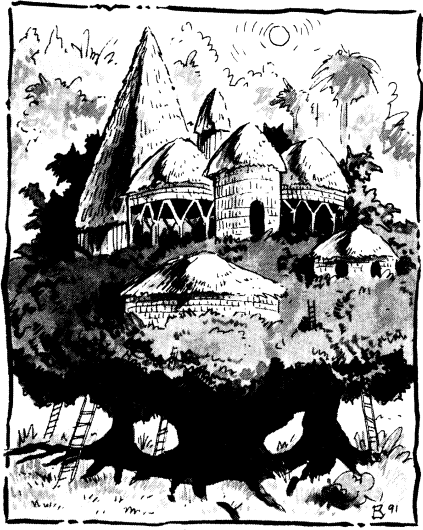
\includegraphics[width=\columnwidth]{images/gulg-1.png}
\end{figure}
\City{Gulg}
{13,500 (80\% humans, 7\% elves, 5\% dwarves, 3\% muls, 2\% half-elves, 2\% thri-kreen, 1\% other).}
{Agafari, copra, feathers, livestock, spices, textiles.}
{Common, Dwarven, Elven, Gulgan.}
{
	The city-state of Gulg sits inside the southern portion of the Crescent Forest, almost directly east of Tyr. Being east of the Windbreak Mountains, Gulg was spared the devastation that the Great Earthquake visited on the cities and villages to the west. That doesn't mean that life in Gulg has remained unaffected by the changes sweeping through the Tablelands. In a few significant ways, Gulg has been changed the most.

	Gulg's sorcerer-queen, Lalali-Puy (LE female champion of Rajaat stage III dragon, defiler 5/telepath 6/arch defiler 5/thrallherd 4/cerebremancer 5/Athasian dragon 2), is the absolute monarch of her realm. Her subjects consider her to be the Oba, the forest goddess. Over the centuries that she's been in power, Lalali-Puy has come to relish the worship and adoration her subjects heap upon her. In fact, though she remembers her origins as a Champion of Rajaat and a sorcerer-queen, she prefers to think of herself as the goddess her people believe her to be.

	To the Oba of Gulg, the abundance of rain---even the violent rain that accompanies a Tyr-storm---is a blessing to Athas. She has proclaimed this blessing to be a gift from the forest goddess. ``No longer will Gulg be solely concerned with the well-being of Gulg,'' the Oba declared to her people. ``Wherever the rain falls, there will the forest grow. And wherever the forest grows, the forest goddess will be there, for all the forests belong to the Oba.''

	Behind the rhetoric, Lalali-Puy actually wants to help restore the vitality of Athas. The Gulgs have always had an enlightened understanding of the interconnected nature of all life, so they've always treated the forest as a precious resource that must be maintained and not depleted. This attitude comes right from the Oba herself, which may seem strange as she is a defiler of extreme power. Since taking over Gulg, however, she has learned to temper her use of defiling magic in favor of keeping her forest healthy.

	Of course, this attitude was one of the contributing factors to the problems with Nibenay. The Nibenese saw the forest as a resource to be exploited, not a living thing that cares for its inhabitants as they care for it. Nonetheless, Lalali-Puy has made the first moves toward a peaceful existence with Nibenay, going so far as to teach the sorcerer-king how to preserve the life-giving environment of the Crescent Forest.

	The Oba's motivation isn't entirely selfless. She believes that when the forests return to Athas she will be deified by all races, just like she's been in Gulg. ``Let Nibenay and Hamanu play as sorcerer-kings,'' she has decided, ``for in the end I will be as a god to all of Athas.''
}
{
	The \emph{dagada} is the single most influential social force on Gulgs outside of the immediate family. The dagada is an extremely close-knit community that shares attributes of both clans and neighborhoods found in other societies. It is similar to a neighborhood in that it is a social organization defined first and foremost by physical proximity. It is like a clan in the role that it plays in acculturating an individual to the values of the society.

	The word dagada is used to describe both a cluster of huts and the people who live there. A dagada can contain up to 100 huts, and typically includes a number of families, though extended families may not necessarily live in the same dagada. Each dagada has a large degree of autonomy in managing its affairs as well as a degree of responsibility for all the members of the dagada. All parents have the burden of raising the young children of the dagada. Elders are responsible for educating the youths as they go. All members have a social duty to care for those who cannot provide for themselves.

	Life has always been more tolerable in Gulg than in any of the other city-states under the rule of sorcerer-kings. In some ways, life has actually gotten better for the Gulgs. The Oba's newfound crusade to restore Athas has made her more forgiving of and generous to her loyal citizens. In the spirit of cooperation, she has selected her best templars to travel the Tyr Region and spread the word of restoration. These templars have a twofold purpose. First, they help show the rest of the Tablelands how to work in harmony with nature, which Lalali-Puy hopes will hasten the reforestation of the world. Second, her templars pass along the tale that the rain is a blessing from the Oba, thereby increasing the number of people who know of and believe in Lalali-Puy.

	Except for the aid these templars have provided to Nibenay, no other city-state has thus far been targeted by the Oba's select force. Instead, the templars visit villages and oasis communities, teaching and preaching as circumstances permit. Some places have welcomed the templars, others have driven them away. Those communities that have actually experienced a Tyr-storm, for example, are quick to attack anyone who claims to be associated with their fearful properties, while those desperately in need of water invite them in.
}
{
\begin{figure*}[b!]
\centering
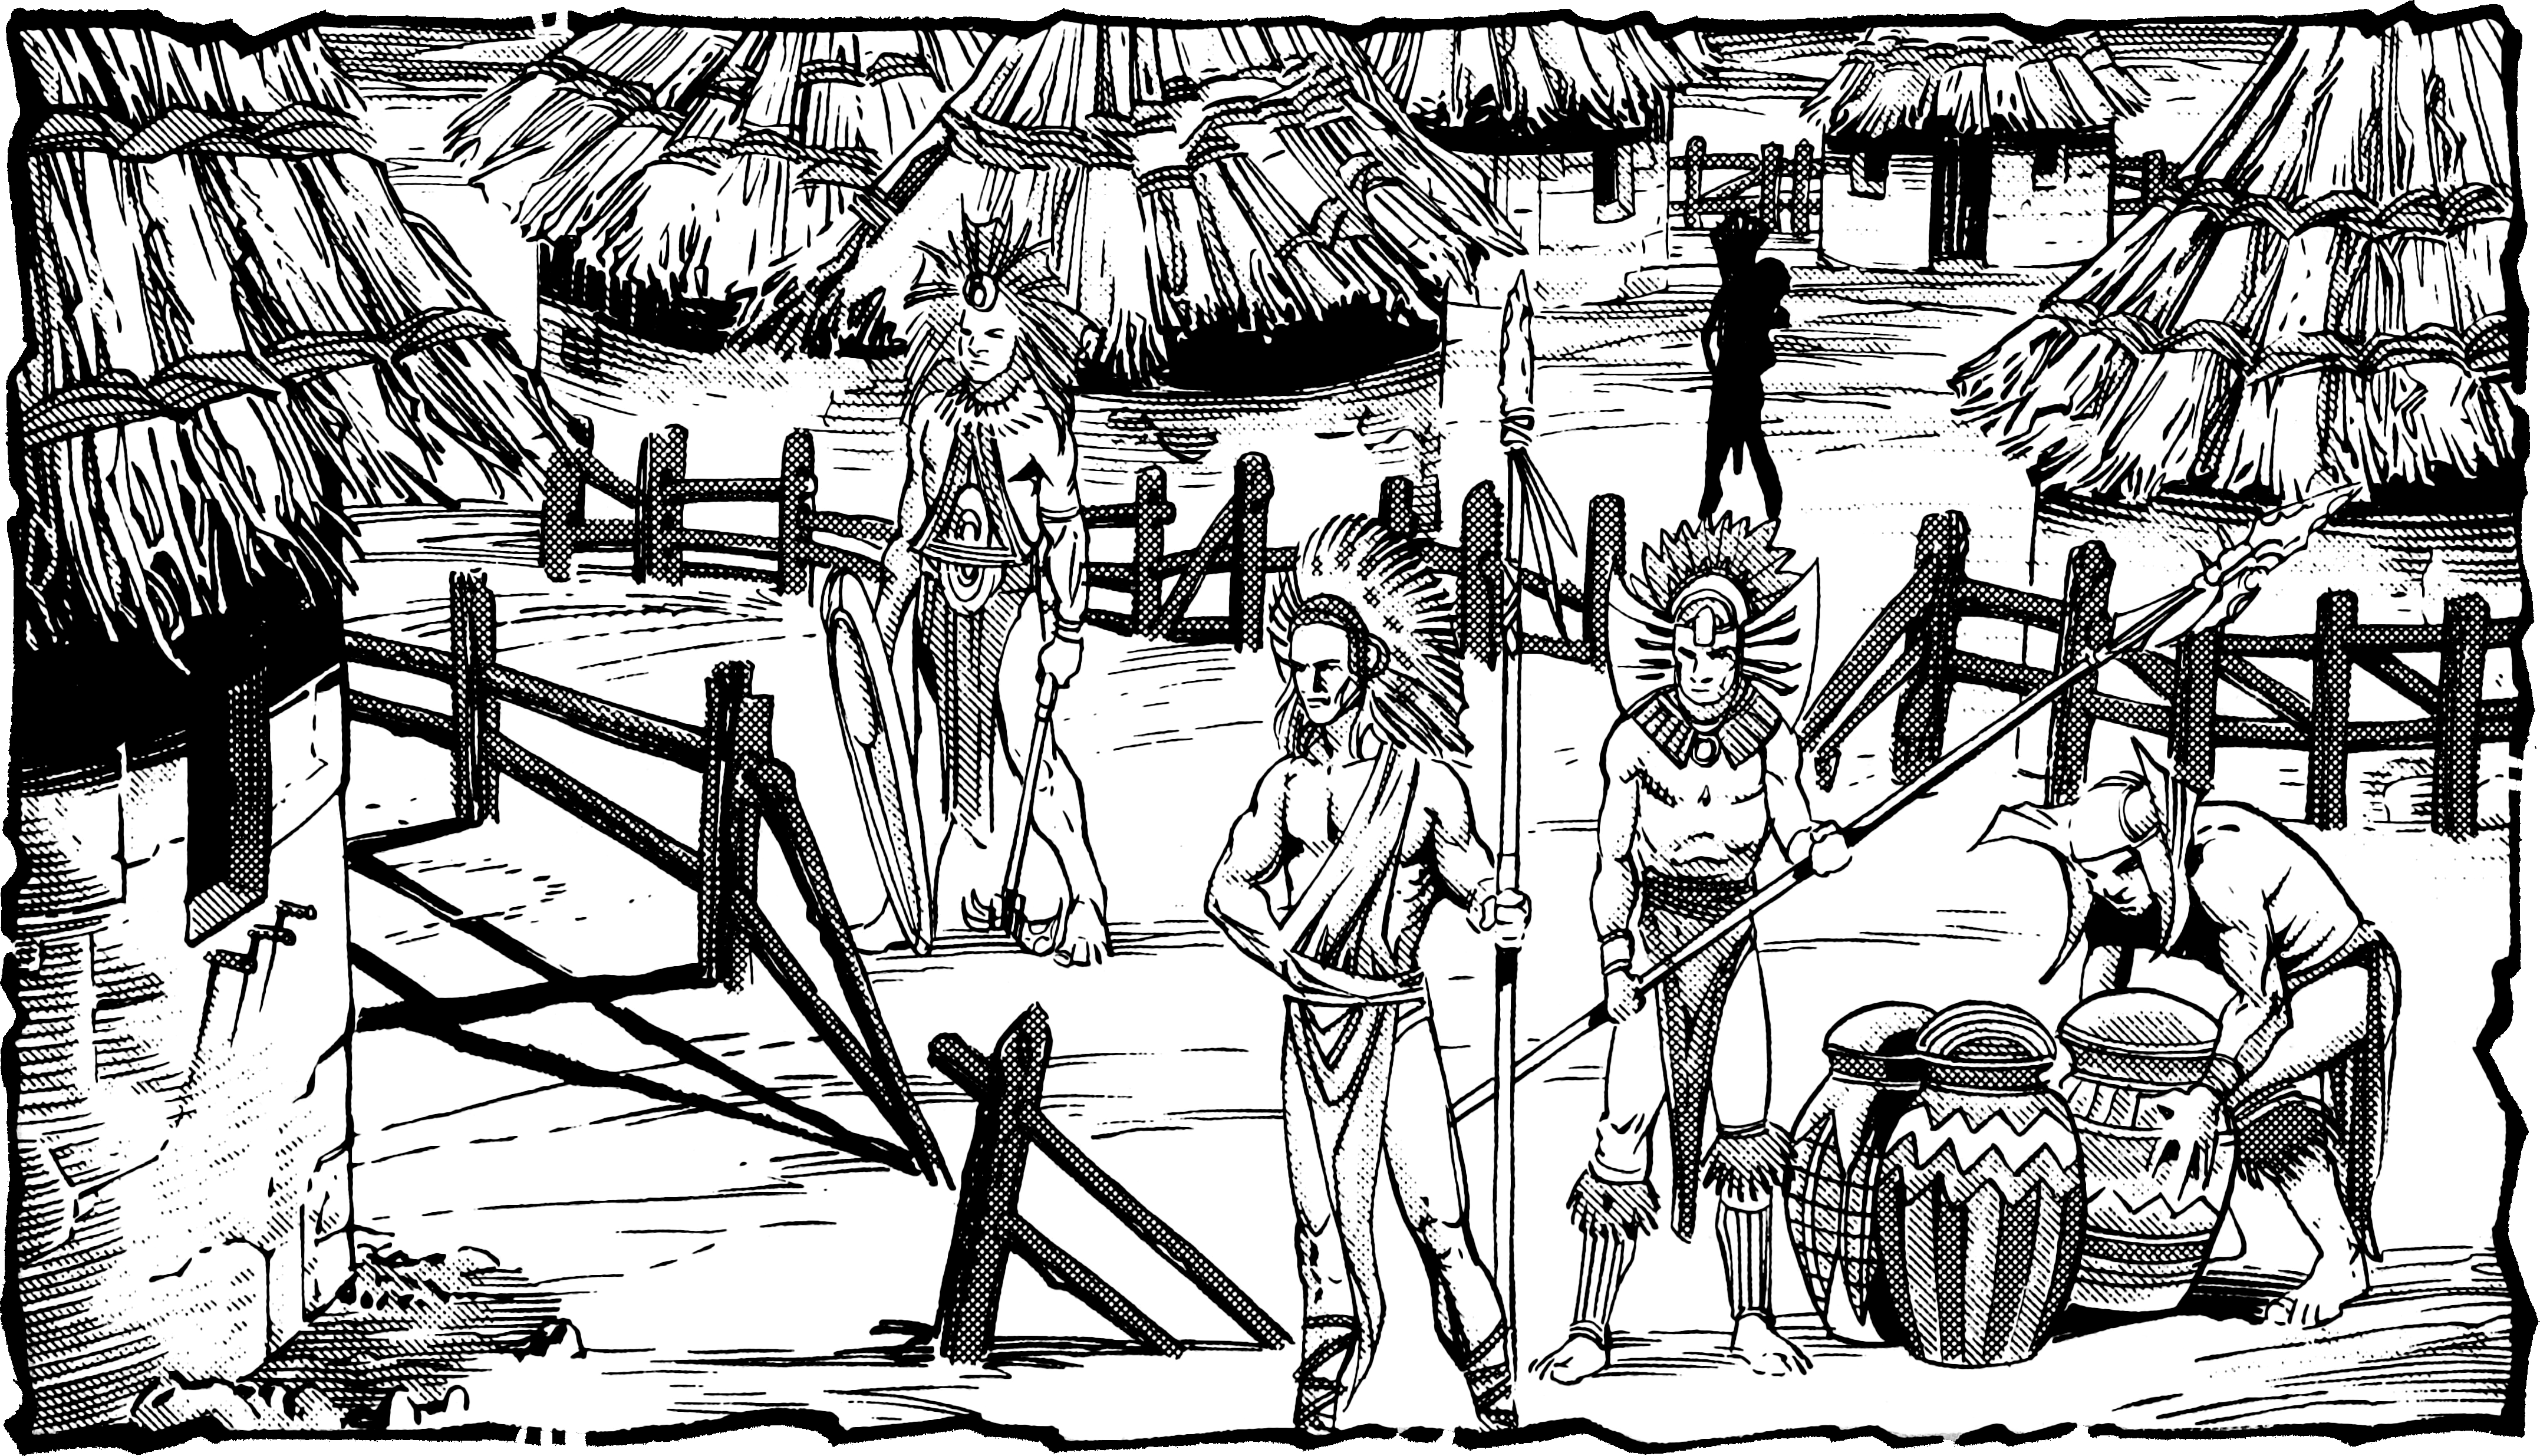
\includegraphics[width=\textwidth]{images/gulg-2.png}
\end{figure*}

	In many respects, Gulg is not like any of the other city-states of the Tyr Region. It's a living city, grown from vines and trees instead of constructed from brick and stone. The outer walls of the city, for example, consist of a thick hedge of thorny trees. The Oba lives in the tallest branches of a huge agafari tree, while her templars inhabit the lower branches. There are no paved or cobblestone roads leading through Gulg. Instead, forest paths and trails wind their way between the trees.

	There have been few major changes in the way Gulg is ruled. The Oba remains the owner of everything, distributing food, water, and other supplies to where they are needed most. Her templars continue to oversee the military, economic, and agricultural aspects of the community on behalf of the forest goddess. Nobility is still an earned position, not one granted by an accident of birth. The nobles hunt the forest for fresh meat, while slaves commanded by the templars gather the wild fruits, nuts, and berries that round out the dietary concerns of the community.
}
{
	\textbf{House Inika}: House Inika, the largest merchant family based in Gulg, is smaller than the typical merchant house. They specialize in small light weight goods of high value, such as spices, gemstones, and feathers from the exotic birds of the Crescent Forest. Inika maintains cordial relations with most of the other houses as it has a reputation for being nonconfrontational. Direct force is rarely used against rivals, with intrigue and economic means being the house's preferred means of strike back at rivals who try to take advantage of the house. The matriarch of the house is Andiama Inika (LN female human, rogue 14/ dune trader 5) who has ruled the house for more than two decades.

	\textbf{Judaga}: Nobility in Gulg is not granted by birth. Instead nobles must earn their position by proving they have the hunting skills necessary to provide meat for the rest of the community. There are several ways in which a citizen can become a noble. One of the most widely known ways a hunter can earn the rank of nobility is by participating in the Red Moon Hunt. During the hunt, prisoners are released unarmed into the Crescent Forest, and a thousand seconds later the hunters are sent after them. If a hunter returns with the head of the prisoners he has earned noble status, which will be bestowed upon him in a ceremony at the next High Sun. The Red Moon hunt is held on nights when the moon Ral is full and alone in the night sky.

	\textbf{The Paper Nest}: The Paper Nest is a secret society comprised of nobles favored by the Oba. The twelve to twenty-four members meet in a secret chamber in the trunk of the Sunlight Home to perform the sacred task of making paper. There is another reason for the group's existence besides making paper. Lalali-Puy attends the meetings and listens as the members debate current problems, offer advice, and present their counsel. At no other time does the autocratic Lalali-Puy allow her subjects to participate in the city's governance.

	\textbf{The Veiled Alliance}: A significant change in Gulg society concerns the Veiled Alliance of the city. Gulg's Veiled Alliance has always actively worked to restore Athas to its verdant glory, never directly opposing the will of the sorcerer-queen.

	Now that the Oba has declared her own intentions for restoring Athas, the two seem to have less to fight over. The Oba has even extended a ``peace leaf'' to the Alliance, calling for the preservers to shed the veil of secrecy and join the forest goddess's quest to save the world. The Alliance hasn't responded yet, but rumors persist that the preservers will soon come out of hiding in the forest city. The Alliance's leader, Aukash-Pad (LG male human, preserver 6/veiled one 5/earth cleric 3/psychic theurge 1), is utterly committed to restoring Athas' life force. If the Oba continues to genuinely work toward that same goal, he may be forced to join with her for the good of the world.
}
{
	\textbf{Losthome (Thorp, 60)}: Losthome is a halfling community deep in the Crescent Forest. The community is less than 10 years old and was formed when the Oba of Gulg attempted to form an alliance with a halfling tribe from the Forest Ridge. An agreement was made, but shortly after the halfling warriors arrived in Gulg, their chief died. The halflings believed that the death of their chief ended the agreement and sought to return to their home, but Lalali-Puy refused to let them go and imprisoned them. Over the years since, most of the halflings have escaped into the Crescent Forest and banded together around their leader, Zivlil (N male halfling, preserver 5/kineticist 3/cerebremancer 2). The halflings maintain no permanent settlement but roam an area of the forest approximately 40 miles wide, in which they have a number of prepared resting areas. The halflings wish to keep their existence a secret to convince the templars of Gulg that they died in the forest. So they kill any nonhalfling who sees them.
}
{
	\textbf{The Drum Circle}: The bard's quarter in Gulg is centered around a dagada called the Drum Circle. The bards of the Gulg specialize in percussion instruments. The most skilled bard in the Drum Circle is considered to be Ken-kenku Vek (NE male half-elf, bard 12). His skills as a drummer and an assassin are legendary.

	\textbf{The Forest Arena}: The gladiator arena of Gulg is located outside the city's mopti wall in the Crescent Forest. Trees and vines intertwine with the arena to give it the appearance of growing from the forest. The floor of the arena is oval shaped, and covered with grass. A number of trees grow from the arena floor; however, none is closer than 6 meters from the arena's walls, to prevent gladiators from using them to escape.

	\textbf{The Grove of Mysteries}: Throughout the forest surrounding Gulg there are a number of forest groves called the Queen's Groves. Entrance into one of these groves without the permission of the Oba is punishable by death. The Grove of Mysteries is the largest of the Queen's Groves and is tended by the druid Extambolan (N male mul, druid 5/grove master 10).

	\textbf{Mopti Wall}: Unlike the walls of other city-states, the walls around Gulg are alive. The Mopti wall is a miles long thorn wall make of thickly packed brambleweed that surrounds the city.

	\textbf{The Seers' Dagada}: When a Gulg shows psionic potential they are sent to the Seers' dagada, where they receive instruction from experienced psions. The teachers are patient and encouraging towards the students. Even those who fail to develop enough psionic potential are not cast out, but remain part of the Seers' dagada performing physical chores for the other members.

	\textbf{Sunlight Home}: Sunlight Home is the name given to the palace of Sorcerer-Queen, Lalali-Puy. Located in the tallest branches of a massive agafari tree, Sunlight Home towers over the rest of the city. Lalali-Puy's palace is rumored to contain dungeons and secret passages that have been carved into the trunk of the massive tree.
}
{
	\item Ngeli is a small boy of ten years old. While gathering cloves in the forest he was attacked and dragged off by a sloth. His parents are distraught and want to see a rescue attempt made to recover their boy, but the ambo of their dagada ruled that the boy was taken by the nature spirits and should be given up to his fate. Ngeli's parents turn to outsiders, the PCs, to secretly bring back their boy.
	\item The berry harvest has finished for the year. The berries had a strange brownish tint, but seemed fine to the taste. But those who have eaten too much of the berries have been having strange reactions. Some exhibit strange new psionic powers, others become sick and die, and some fall into a suggestive state and will do nothing but what others tell them to do.
	\item Alexia Vordon trades for spices with Gulg. She feels that her house trades at a disadvantage by being forced to deal with the templars. If she can make contact with a member of the spice gathers she is convinced that she will have a better understanding of how good the year's harvest has been and be in a better position to negotiate with the templars. Alexia hires the PCs to sneak her into the city and help her try to befriend someone from the spice gatherers dagada.
	\item Rumors in the neighborhood have begun that a teenage girl is really a witch. The wild rumors began when the girl started wearing a veil that covers her face leaving only her eyes showing. Many hot-headed, superstitious members of her dagada are contemplating drastic actions against the girl. The PCs will have to find some way to stop these rumors. The truth is that the girl has experienced her first heavy case of acne. Unsure of what is really happening to her, and fearful that others will reject her because of her affliction, she hides behind the veil, refusing to remove the veil and revealing her affliction to anyone.
	\item The PCs are invited on a hunt with a group of nobles from Gulg. The nobles seek to test the PCs hunting skills. They hang back letting the PCs take the lead, while hunting a dangerous beast, such as a klar.
	\item The templar, Kampala, has a feylaar as his fetish. When visiting a small client village, he summons the totem spirit, only to have it break from his control and go on a rampage.
}
\City{Nibenay}
{24,000 (60\% humans, 12\% half-giants, 10\% dwarves, 10\% elves, 4\% half-elves, 3\% muls, 1\% other).}
{Rice, timber, hardwood, weapons, copper.}
{Common, Dwarven, Elven, Nibenese.}
{
	Nibenay has been affected by the monumental happenings of recent months, for the Shadow King has changed his approach to ruling the masses and dealing with the neighboring city-states. Like Hamanu and Lalali-Puy, Nibenay (who shares the same name as his domain) witnessed the deaths of the Dragon and the other sorcerer-kings.

	He saw Rajaat reach out from beyond the veil of Athas to wreak vengeance against those who betrayed him. He also saw Rajaat defeated by the efforts of lowly mortals from the city of Tyr. In the wake of these signs and portents, Nibenay realized it was time to reconsider how best to rule his city, for the time for change had come.

	The city-state of Nibenay is located east of Tyr at the northern tip of the Crescent Forest. It barely felt the effects of the Great Earthquake, as it was protected by the Windbreak Mountains. Nibenay has also thus far been spared from Tyr-storms and the growing unrest spreading throughout the Tablelands. If the Shadow King has his way, none of these problems will ever reach his domain.
}
{
\Figure{b}{images/nibenay-1.png}

	Though there have been no major changes to life in Nibenay, enough strange occurrences have been worked into the routine to put a different spin on the city-state. For example, average citizens and even powerful nobles never expected to see the Shadow King, let alone attend one of his courts. Now the Shadow King regularly makes public appearances and shows an active concern for his community. This doesn't mean that life is any harder or easier than it's always been. It's just different. If a citizen or visitor breaks a law and can't afford to bribe a templar, then that citizen or visitor is still going to end up in Nibenay's slave pens.

	The other major change is the city's outlook on matters of a martial nature. The Shadow King and his templars seem to be concentrating much of their efforts on bolstering Nibenay's military might. The army regularly practices in the arena and patrols of the surrounding countryside have increased dramatically. In addition, free citizens and nobles have been ordered to serve in Nibenay's defense. Templars are busy organizing them into part-time militias and regimenting training sessions.

	What the Shadow King is truly concerned about, besides the unrest and upheaval that seems to be spreading throughout the Tablelands, are the rumors claiming that Dregoth has returned. Nibenay knows how powerful the sorcerer-king of Giustenal was. Dregoth was second only to Borys the Dragon in power. If Dregoth and his city have somehow come back from the dead, Nibenay wants to be prepared.

	After all, Nibenay's city-state is one of the closest to the ruins of ancient Giustenal, and he has no intention of losing his domain to a rival that was destroyed two millennia ago.
}
{
\Figure*{b}{images/nibenay-2.png}

	The sorcerer-king Nibenay (LE male champion of Rajaat stage IV dragon, defiler 5/seer 5/loremaster 10/cerebremancer 10/Athasian dragon 2) used to stay behind the scenes. He was called the Shadow King because he rarely left Naggaramakam, his walled sub-city. His templars, who are all female, ran the city with skill and great care. Now, however, the Shadow King has become more prominent.

	In the past, the average free citizen could hope to see King Nibenay once or perhaps twice in an entire lifetime. Since the time of the Great Earthquake, Nibenay has taken a more active role. He still allows his templars to deal with the daily business of government, but now Nibenay has turned his attention away from the mysterious scholarly pursuits that once occupied his time to hold court for the city's nobles and free citizens.

	Nibenay's military might was never a question, but it also was never a major concern of the Shadow King. Now he actively seeks to understand his forces and looks for ways to improve their might and readiness. While the city used to appear to be secure in its own position, it now seems to be gearing up to battle an enemy that only the Shadow King knows about. The problem is that the enemy is change, and no army that Nibenay raises will be able to stop its relentless tide.

	In the wake of all this upheaval, Nibenay's nobles continue to care for and maintain the bubbling springs that surround the city. They don't know what to make of the Shadow King's sudden interest in the business of the city, but many of them are seeking ways to improve their own positions by getting closer to their once-elusive king.
}
{
	\textbf{Poortool's Horde:} Lead by the half-Elven preserver Poortool (LN male half-elf preserver 5/seer 3/cerebremancer 5), the Horde is a raiding tribe to the east of Nibenay. Poortool is a renegade from the Veiled Alliance who seeks to study magic without any restriction that the Veiled Alliance or sorcerer-king Nibenay may apply. He has created a community for likeminded preservers in a village in the foothills of the Black Spine Mountains. He has also allied with the gith of the Black Spine Mountains who provide guards and raiders for his tribe. Poortool seeks to make it difficult for members of the Veiled Alliance in Nibenay to convince its members to leave the Alliance and join him.

	\textbf{House Shom:} House Shom is thought to be the oldest merchant house operating in the Tyr region. For centuries the house amassed great wealth through aggressive trading. However, now the House is seen as passive and decadent. The Shom family members are almost never seen in public and have little to do with the daily business of the house. Instead the family members live decadent lives in their palaces, engaging in expensive parties and balls. The running of the trading house is left to the house agents. Most of the agents place their interests ahead of House Shom's interests, and there is much infighting between agents. This has lead to a decline in the House's prospects over the past few decades. Only the house's immense wealth has saved it from collapse already. House Shom is known to use non-human guards on its caravans and as raiders against other merchant houses, including thri-kreen packs and belgoi tribes. The house is currently ruled by Temmnya Shom (NE female human, defiler 15). Her younger brother, Jebea Shom (LN male human, rogue 3/fighter 2/dune trader 1) has begun a reform movement to straighten out the family's problems, but his popularity threatens Temmnya's position. She has contemplated disposing of him if she can do so without her involvement being discovered by other family members.

	\textbf{Sky Singers:} The Sky Singers elf tribe maintains a permanent market in the Hill District of Nibenay. It is the only known instance of a permanent Elven market. The market is filled with goods of all kinds from the rare to the common. The Sky Singers have a reputation of offering quality products that were not stolen from their previous owners, unlike most Elven tribes. While the tribe numbers over 3,000 members, much of the time the elves are off wandering, leaving only a dozen or so elves to tend the marketplace. But when the tribe returns, the Sky Singers' market takes on a festive atmosphere.

	\textbf{The Veiled Alliance:} Nibenay's Alliance has an utter hatred of defilers. This has led to a rare commodity beneath Athas' crimson sun-idealism. With the help of an ancient spiritual force known as the zwuun, which resides in the hot springs outside the city, the Alliance does what it can to protect wizards who use preserving magic. The Alliance doesn't feel it can oppose the Shadow King directly, so it directs its activities against lesser defilers. Thagya Phon (LN male human, preserver 7/veiled one 10) leads the Nibenese Alliance, though his health has begun to fail him in recent years. He has two goals he wishes to accomplish before he dies: He longs to discover what Nibenay's scholar slaves have been working on in the Naggaramakam, and he has a dream of mounting the Shadow King's head on the obsidian pedestal that rises from the floor of his spartan quarters.
}
{
	\textbf{Cromlin (Hamlet, 150):} The trading village of Cromlin sits on the shores of the Silt Sea, northeast of Nibenay. House Shom runs the village, though House M'ke has a sizable operation as well. Together they handle the vast majority of trade from the north, as traders attempt to bypass the chaos of Raam. Cromlin traders use silt skimmers to navigate the silt shoals, keeping the trade route to Break Shore open. The shoal navigators of Cromlin are in high demand, for they are among the select few who can lead silt skimmers along the buried paths.

	Cromlin is a wild place, full of people who are too untamable to live in the cities. Thieves of all sorts reside in the village. Silt pirates use it as a haven and other scoundrels and restless souls are drawn to its sandy shores. Master trader Hurdll Crost (N male human, bard 10/dune trader 5) and his agents turn a blind eye towards shady characters as long as they remain to do business in his village.

	\textbf{Salt View (Small Village, 550):} Nestled in the Mekillot Mountains, Salt View is a chaotic sprawl of tents and buildings located within a large cavern on the mountain's eastern face. Ex-slaves of all races fill the community. The tribe originally practiced raiding as its primary occupation, but today it is known for a lavish form of storytelling called theater. Salt View's traveling theater troupes are welcome across the Tyr Region, though they present themselves as free merchants from the independent House Fyra (a cover for Salt View activities). The troupes perform for caravans, at oasis villages, and even in the city-states of Tyr, Nibenay, and Balic.

	\textbf{Vavrek (Thorp, 200):} Vavrek is typical of the small farming villages located throughout the Fertile Crescent. The village is located southwest of Nibenay within sight of the Crescent Forest. The villagers grow vegetables, mostly soybeans. The land the village is built on is owned by the Koelse noble family, to which the villagers must pay rent. The village is administered by a templar-wife of Nibenay named Sonyalah (NE female human, templar 5/wife of Nibenay 3).
}
{
	\textbf{The City Reservoir:} The Shadow King had this enormous stone cistern constructed centuries ago to supply the city with water in the event of a siege. The top of the reservoir is covered and a lush garden, maintained by the templars, grows on top of the reservoir.

	\textbf{The Coliseum:} The coliseum rises above the dilapidated buildings in a rundown part of the city. The size of the arena is immense, taking up four city blocks and rising six stories high. It is an ancient building and it is said that not even the Shadow King knows when the coliseum was built and by whom. Elaborate carvings and etchings cover the coliseum's stonework. The square shaped arena floor stretches almost a quarter of a mile across.

	\textbf{Monasteries of the Exalted Path and of the Serene Bliss:} Nibenay has a tradition of monasteries. The two orders are called the Exalted Path and the Serene Bliss. The monks pledge loyalty to the King and their teachings include the quiet acceptance of authority, so the templars tolerate them. They are treated with great respect by the citizens. The monks live very aesthetic lives, tending gardens and mediating. Many of the monks, especially those of the Exalted Path, study psionics. The Exalted Path consists entirely of male monks and is led by Thong Nal, (CN male human, air cleric 3) who encourages the study of psionics at his monastery. Other monks become artisans who specialize in the carving of the images that cover the buildings of Nibenay. The Serene Bliss is an all female order and is led by the abbess Au Treng (LN female human, cleric 4).

	\textbf{Naggaramakam:} The Naggaramakam is a walled forbidden inner city where the sorcerer-king Nibenay lives with his templar-wives. Only templars are permitted to enter and leave the Naggaramakam. While slaves are permitted to be brought into the Naggaramakam, once inside they are never allowed to leave. No free citizen is ever allowed to see the inside of the Naggaramakam. The sorcerer-king's palace is said to be carved into a stone relief of the Shadow King with dancing women, representing his templar-wives, strung together as if they were his hair.

	\textbf{The Omnipotent Receivers:} A line of large statues of sorcerer-king Nibenay stand on each side of the main road leading to the city. The statues are called the Omnipotent Receivers as it is believed that King Nibenay sees all that the statues see.

	\textbf{The Plain of Burning Water:} The city of Nibenay is situated on the border of a large area of hot springs. Called the Plain of Burning Water, the hot springs provide the water needed by the citizens of Nibenay. Each noble house owns at least one of the hot springs which is the source of much of the wealth of the nobility.

	\textbf{Sage's Square:} Sage's Square is the largest open area inside of the city. The grand emporiums of all the dynastic merchant houses are located around the square and are the center of trade in Nibenay, where almost anything can be purchased. The square was named Sage's Square because scholars and sages use to gather under the shadow of the huge agafari trees that grew in the square, and debate philosophy. This tradition ended only a few years ago when a renegade defiler, fleeing the templars defiled the trees. King Nibenay had the dead trees removed from the square, and ordered that no other trees be planted in the square as a public reminder of the danger of renegade defilers.

	\textbf{The School of Augurs:} The school of Augurs is the largest school for psionic instruction in Nibenay. The head master is a dwarf named Djef, who developed a scheme to help support the school by hiring out its students to transfer telepathic messages and to teleport-deliver small parcels.
}
{
	\item A disguised dray agent has entered Nibenay seeking to make contact with nobles disgruntled with the Shadow-King's rule. The dray tries to gather together as many nobles as possible so that when Dregoth makes his attack on Raam, he can start a rebellion in Nibenay to distract the Shadow-King from interfering in Dregoth's plan.
	\item The templars attempt to ambush a cell leader of the Veiled Alliance who they believe is staying at the same inn as the PCs. During the templar raid, one of the PCs is mistakenly identified as the Veiled Alliance member. Capture means execution, so the PCs must flee. If the PC makes it out of the city, his problems are not over. Because of the secrecy of the Veiled Alliance, the subordinates of the cell leader have never met him before. When the templars identify the PC as the cell leader, the other members assume it to be true. When the PC flees the city the cell members attempt to enforce Requital, believing the PC has tried to resign from the Veiled Alliance.
	\item Ramai is a templar of Nibenay, who is responsible for interrogations. Dedicated and highly skilled in all manner of interrogation and torture techniques, she holds some respect within the templar hierarchy. Her career appeared promising until one day, inexplicably, Ramai fell in love with one of her victims, a young man named Tongkol. Unable to bear the thought of Tongkol suffering under torture but also realistic enough to know they can never be together, she assigns the PCs the task of spiriting Tongkol out of the city. Ramai will not offer the PCs any direct help, but can give them information to help them succeed. If the PCs fail and are captured, Ramai will deny any involvement with the PCs and see that they are executed quickly to silence them.
	\item Gith raiders have discovered a previously unknown ancient catacomb that allows them to enter the city undetected. They raid some dwellings in the city and attempt to flee back the way they came. But undead that were angered by the gith's trespass have arisen and prevented the gith from getting out of the catacombs. The PCs are sent into the catacombs after the gith and must also face the undead horrors.
	\item One of House Shom's merchant forts has been overrun by gith. The PCs are hired to lead the assault to retake the desert fortress.
	\item A preserver of the Veiled Alliance asked the zwuun for help on his latest research. The zwunn's answer directed the preserver to the site of ancient ruins that overlook the road to North Ledopolus where he could find what he sought. Unsure if the zwuun was being mischievous or not, the preserver sends the PCs to scout out the ruins.
}
\begin{figure}[b!]
\centering
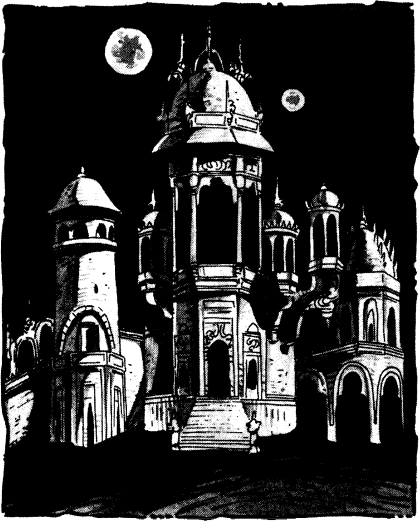
\includegraphics[width=\columnwidth]{images/raam-1.png}
\end{figure}

\City{Raam}
{40,000 (40\% humans, 20\% dwarves, 15\% elves, 10\% muls, 5\% half-elves, 5\% half-giants, 4\% thri-kreen, 1\% other).}
{Silver, gems, flint, jute, silk, textiles.}
{Common, Dwarven, Elven, Raamite.}
{
	Shortly before the day of the Great Earthquake, the sorcerer-queen Abalach-Re was killed in battle with Sadira of Tyr. When the news reached Raam, it was the spark that ignited the fires of anarchy, and now Raam burns. But Raam was a city on the brink of revolution even before the death of its queen. Since Abalach-Re's death, the city has collapsed into chaos. Various factions have grabbed whatever power they could, and Raam teeters on the brink of civil war.
}
{
	Raamish society revolves around a caste system. Each citizen is born into a caste and can never leave it. Members of one caste cannot marry or associate with others from another caste without becoming unclean. Caste and race are not related, and a member of each race can be of any caste.

	The highest caste is made up of priests. This caste includes clerics and druids, as well as teachers, scholars and wise men. Members of this caste wear white garments to distinguish themselves.

	Below the highest caste, is the vizier caste. The templars and soldiers of Abalach-Re fall into this caste. The members of the vizier caste typically wear silk clothing dyed a variety of colors.

	The next caste includes the majority of the nobles of Raam, as well as artisans, and tradesmen. Wealth has no affect on one's caste. The richest tradesmen will never rise above his caste. This caste typically dresses in clothing made of less expensive material than the silk worn by the vizier class.

	The laborers caste is the largest caste and the lowest. It includes all servants and unskilled workers as well as the vast numbers of slaves. Laborer caste members wear simple white linen clothing.

	Below the laborers caste are the truly desperate. Outcastes are those who most handle dead animals and people. Butchers, morticians, and tanners are all included in this caste. They are considered so unclean that they must live outside the city to prevent them from polluting the rest of the citizens.

	The environmental disasters of recent months have had very little impact on Raam. The Great Earthquake was barely perceived, for it caused little damage and no deaths. No Tyr-storm has yet visited the city-state, so Raam's residents have yet to experience the devastation that such a storm can inflict. The death of Abalach-Re and the resulting struggle for power, however, have caused more death and destruction than any force of nature.

	Raam has been divided into armed camps controlled by greedy, power-hungry warlords. Some call themselves templars, others nobles, liberators, or merchant lords. All are raiders and bullies, seeking to use strength as a means of control.

	These armed camps don't even make a pretense of peaceful coexistence. Skirmishes over disputed territories are constantly being fought, as are battles over caches of weapons or supplies-even just to determine which side is stronger! It won't be long before all-out war breaks out to see if one leader and his faction can conquer the others and restore order of some sort to the city. This war, of course, may simply wind up destroying Raam and reducing the verdant belt it occupies to a wasteland.

	Understandably, the free citizens live in a constant state of fear. They have nowhere to go, nowhere to turn to, and conditions within the city become more terrible every day. Some citizens have appealed to one faction or another, offering to become indentured slaves for the protection and sustenance offered by the vying warlords.

	Every day, more and more citizens surrender their freedom in exchange for a safe place to sleep, a cool drink of water, and a bit of food to fill an aching stomach.

	The slaves of the city have fared even worse than the free citizens. Their masters have been replaced by heartless owners who treat the slaves no better than living tools that can be replaced when they break. Some slaves, embracing the legends of Rikus, Neeva, and Sadira of Tyr, have rebelled, using the opportunity presented by the chaos. One group has come under the leadership of a gladiator named Korno (CN male mul, barbarian 1/gladiator 4/arena champion 4). Between Korno's military daring and expertise and the cache of weapons his followers found in one of Abalach-Re's many hidden treasuries, this group of slaves has set itself up as another armed band in a city of gangs. Korno has called for all slaves to join his community, for when they have the numbers to go along with their dreams they will rise up and overthrow all their masters. Korno, however, is as cruel and ruthless as any of the other leaders of the armed bands. The slaves that have flocked to his side continue to be treated as slaves, working to make life easier for Korno and his best warriors.

	With food and water in short supply and violence rampant in the streets, it is little wonder that the people of Raam are turning to anyone or anything that claims to have a solution. In this volatile environment, revolution seems to be inevitable. What the outcome of such an event will be is unknown, but by all indications it will be bloody in the extreme.
}
{
\begin{figure*}[b!]
\centering
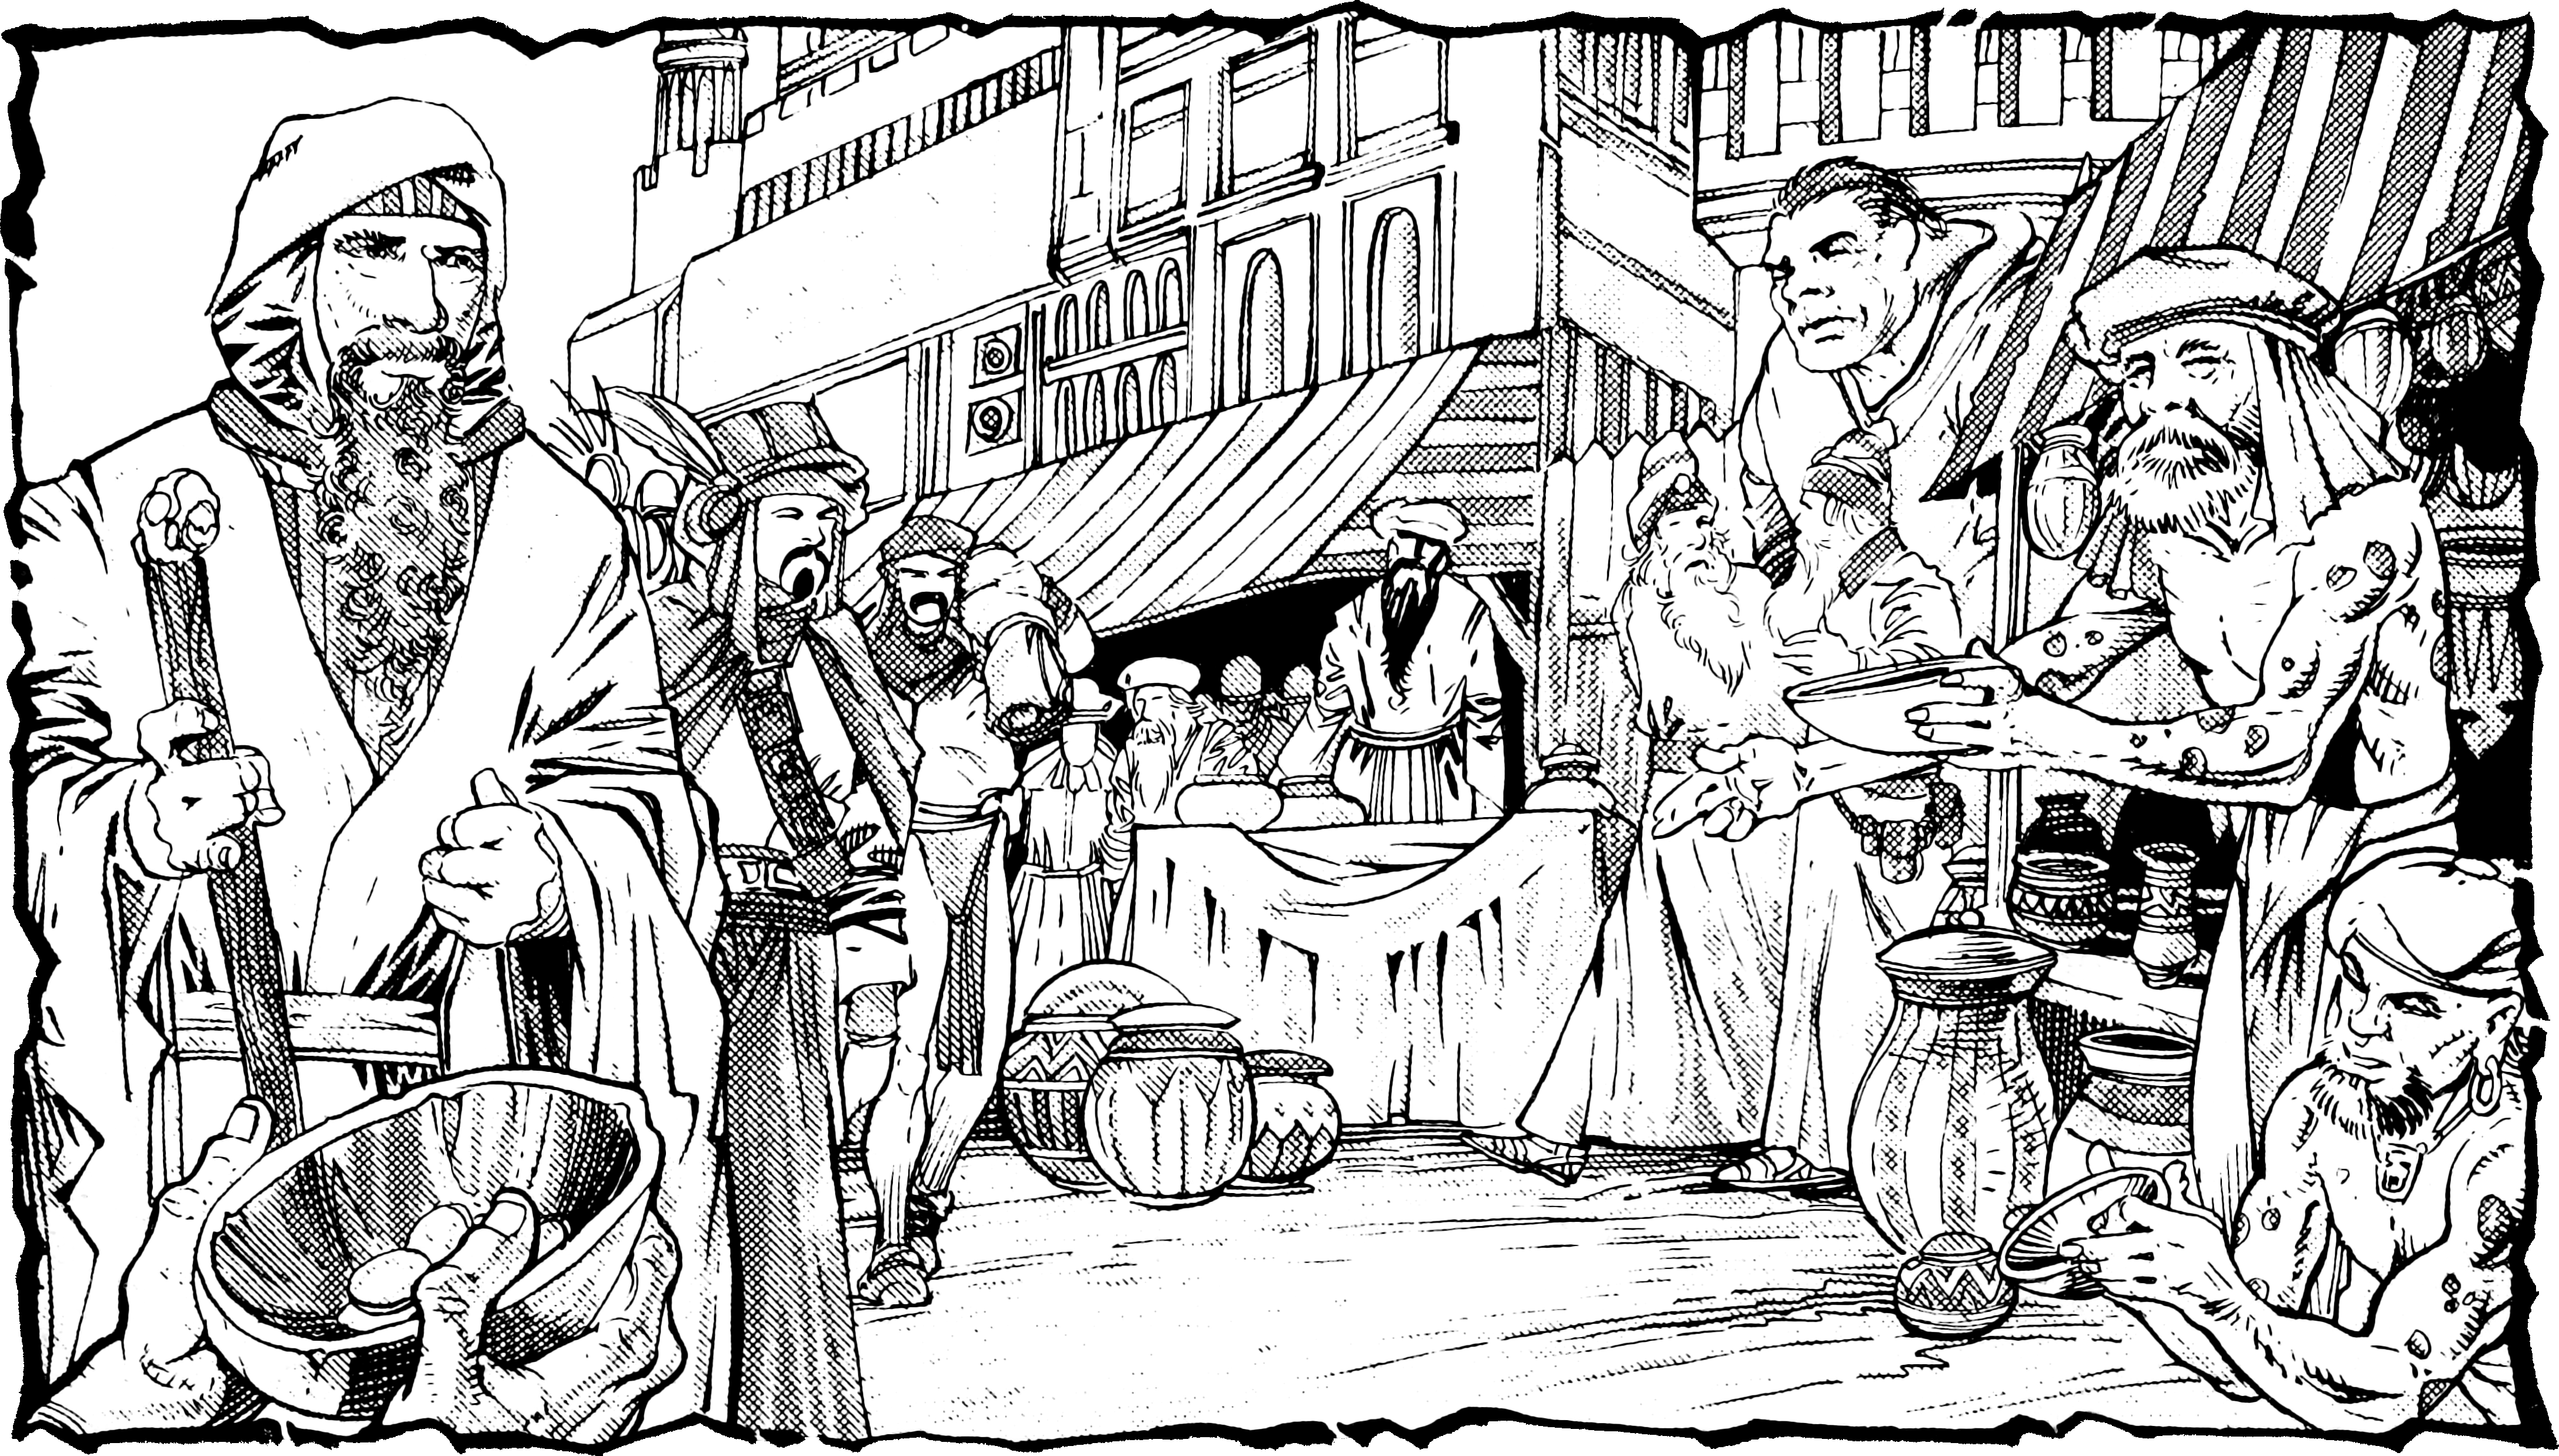
\includegraphics[width=\textwidth]{images/raam-2.png}
\end{figure*}

	The government of Raam still exists, but it has almost no power in the face of the violence and chaos ravaging the city. The templars who haven't fled in fear or tried to hide among the populace as regular citizens continue to administer the city, but it is clear the city no longer functions the way it used to. These templars have only their bureaucratic skills to fall back on, as their ability to use priestly spells vanished with Abalach-Re's demise. The templars continue to call for the worship of Badna, the mysterious (and imaginary) being the sorcerer-queen claimed to receive her powers from. Most people ignore these calls to worship, for they never believed in Badna anyway.
}
{
	\textbf{Leviath the Calm}: Leviath the Calm (LN male half-giant, shaper 9) is an unusual half-giant who speaks of peace and tranquility to all who would listen. His words are spoken with kindness and sincerity, and have had a profound effect on the masses, among which he has developed a large following. Despite his large size and strength Leviath is said to have never raised his voice in anger or struck a blow to harm another living creature.

	\textbf{House M'ke}: The merchant houses have taken one of two tacks regarding conducting business in Raam. The first option, chosen by the vast majority of merchant houses, was to get out of town and take their business elsewhere. The second option, embraced by House M'ke as a prudent enterprise that will ensure its own survival, was to seize control of as much of the city as possible. House M'ke and its army of mercenaries now control most of the merchant district. Armed bands wearing House M'ke's colors periodically sweep through the city, looting and pillaging until they gather enough goods to fill a caravan. This caravan then sets out across the Tablelands to conduct trade as any merchant house caravan would. Only in Raam does House M'ke behave like a conquering army of raiders-because in Raam, that's what House M'ke has become. A few of the more daring (or desperate) merchant houses return to Raam from time to time to test the climate, but they usually wind up losing their goods to one or more of the armed camps seeking dominance in the city.

	\textbf{Night Runners}: The strangest group to stake a claim in Raam's power vacuum is the elf tribe known as the Night Runners. Prior to Abalach-Re's death, the Night Runners maintained a small presence in Raam. Now this group of elves-which specializes in the ``shadow arts'' of espionage, assassination, and extortion-has decided to take a more active role in Raam society. A large portion of the elf quarter and the tradesmen's district has been taken over by the Night Runners. Besides holding and expanding their own territory, the Night Runners continue to sell their unique services to those who can afford them---including noble houses, merchant camps, and even templar domains. In the end, the Night Runners plan to control the entire city, making it the first elf city in thousands of years. Until then, the elves don't mind working for the bands they're competing with, for it gives them an easy way to keep tabs on how the factions are doing.

	\textbf{Nobles}: One of the largest groups claiming dominion over sections of Raam is the noble families. Like the raiding tribes of the sandy wastes, the nobles pillage and plunder for the things they want and need to survive. The nobles have expanded their areas of control. While each family started with a small piece of land and the road adjoining it, those with the power and audacity to press their advantage have grabbed whatever they could hold onto. Like the raiding tribes, the noble camps are savage, ruthless, and have only their own interests at heart.

	\textbf{Prophets of Dregoth}: Strange figures with bizarre accents who hide their features beneath many folds of robes preach of Dregoth the Savior. These prophets claim Dregoth is a god who will bring salvation to Raam if they lay down their weapons and accept him.

	\textbf{Templars}: The main body of templars occupies one camp, centered in the templar quarter of the city. Various rogue templars command smaller parts of Raam, claiming from as little as one building to as many as several blocks as their personal domains. They defend these domains with troops that were once loyal to Abalach-Re but now follow their templar commanders.

	Under Abalach-Re's reign there were two organizations of templars assigned to police the city. The mansabdars were the public force. They were assigned to guard and patrol duties. Though the larger of the two police forces, the mansabdars were corrupt and many were incompetent. The kuotagha was the secret police force. These ruthless enforcers were tasked with administering justice as they saw fit. Disguised as merchants and artisans, they moved freely among the population spying out sedition and unlawful behavior. When they judged someone guilty, the kuotagha executed the suspect without trial, immediately and by surprise. All kuotagha members carried a special garrote called a ghi, for use in such situations.

	\textbf{The Veiled Alliance}: The turbulent conditions in Raam haven't made it any easier for the city's Veiled Alliance. The preservers continue to operate in secret, but the contacts they once had in all levels of government have been lost. Nanda Shatri (LG female human, preserver 7/telepath 4/veiled one 10) continues to lead the Alliance and still seeks to become an avangion so that she can help restore Athas' lost vigor. However, beyond the vague rumors that Urik's Alliance had created such a being some years back, Shatri is no closer to her goal than she was a decade ago. She has considered siding with one of the armed bands in order to assure the safety of her people, but she has yet to determine which band to approach. Her reluctance to make a decision might be her undoing, for the Prophets of Dregoth have begun making overtures to the Alliance that the members find very appealing. In fact, the Prophets have also promised that Dregoth can help Shatri with her research into the avangion transformation process---a promise that she is seriously considering accepting.
}
{
	\textbf{Daro (Thorp, 300)}: Daro was a center of agricultural administration, used to oversee the slaves working the fields of Raam. After the death of Abalach-Re, templar Avish Thira seized control of Daro, instituting martial law which prevented the chaos that swept the rest of the city-state from reaching Daro. Under Avish Thira the village no longer is concerned with agriculture. The fields have been allowed to become fallow and most of the hundreds of field slaves have been freed, actually expelled from the village since Thira could not feed them. Thira supports himself and his guards by sponsoring raids into Raam.
}
{
	\textbf{The Benevolence Center}: The Benevolence Center is the name of a large housing complex for the elderly.

	\textbf{The Consecrated Sepulcher of Badna}: The massive Consecrated Sepulcher of Badna is one of the most majestic buildings in Raam. The Sepulcher is a mausoleum where the remains of the last 30 generations of favorite husbands of sorcerer-queen Abalach-Re were laid to rest.

	\textbf{The Crematory}: The stark granite walls of the Crematory tower over the slums outside the western wall of Raam. There are no windows in the entire building. A large chimney rises from the back of the building, emanating a thick column of smoke. Only outcastes are considered suitable to handle the remains of the dead, and as such the crematory is staffed completely by outcastes. Members of the rest of Raamish society spend as little time as necessary in the Crematory for fear of being contaminated.

	\textbf{The Gallery of the Seven Stars}: The Gallery of the Seven Stars houses the works of Raam's finest sculptures. Built of white rock, the Gallery is decorated with ornate murals and minarets. The museum contains seven star-shaped display halls where magnificent sculptures are displayed.

	\textbf{Natural Arena of Raam}: Raam's gladiator arena is a naturally formed amphitheater formed between two hillocks, outside of the city's walls. Wind and time have carved one of the hillsides into natural seating areas of rust colored rock. The arena floor is a rough oval and has a floor of red sand. A natural crevasse separates the arena floor from the seating area. Known as ``The Maw of Raam'' the chasm runs the full length of the arena floor, and is rumored to be almost 60 meters deep. The bottom of the Maw is difficult to see because of the wild brambleweed that grows within. On the second hillock, the side that forms the back of the arena is a sheer granite wall. The hillock contains many tunnels and secret passages that end at observation spots throughout the hill. It was from here, hidden from the sight of the populace that Abalach-Re and her templars watched gladiator contests.

	\textbf{Psiumarkh}: The Psiumarkh has been the most prestigious of the psionic schools in Raam. It can trace its founding back to the founder of modern psionic principles, Tarandas over 900 years ago. The Psiumarkh has always maintained strict neutrality in the struggles that afflict Raam, allowing them not to anger any of the city's powerful factions.

	\textbf{Royal Barracks}: Located within the Palace district of Raam, near the Ivory Palace, the Royal Barracks is a multi-storey building used as a military barracks for the elite warriors and officers of the Raamish army.

	\textbf{The Ivory Palace}: Abalach-Re ruled Raam from a beautiful palace of ivory and alabaster. Built upon a knoll and surrounded by a series of defensive ditches and walls, Abalach-Re prevented most of her subjects from approaching her palace. Since her fall, various noble factions have attempted to seize and/or loot the palace. Their resulting struggles have destroyed most of the palace. Recently rumors of a curse affecting those who enter the ruined palace are beginning to spread.

	\textbf{Wrestling Pits}: Located near the Elven market, the wrestling pits are used for legal and illegal matches.

	\textbf{The Yellow Monastery}: The Yellow Monastery houses a group of monks who focus their study on telepathic psionic powers. Under the rule of Abalach-Re, the monastery was seen as a symbol of resistance to her rule, as the monks were opposed to slavery as well as the use of magic of any kind. Since the sorcerer-queen's fall, the monks have tried to protect those who live near the monastery against the chaos that has engulfed the city, but to little effect. They are rumored to have befriended the half-giant Leviath the Calm and his followers.
}
{
	\item An undead war beetle is no longer under the control of its handlers and goes on a rampage. Something has wrestled control of the beast away from its handlers and the PCs must board the undead war machine and face whatever it is.
	\item The situation in Raam is getting desperate. One morning a large group of members of the laborer caste gathers in front of the PCs' dwelling. Desperate for food, they believe the PCs are hoarding food. After building up their courage, the rioters attack the dwelling. The rioters are lead by a deranged woman who clutches the undernourished body of a small baby. In her desperation, the woman deludes herself into thinking the baby is still alive. Even if the PCs drive off the rioters, rumors of their hoard of food spread quickly around the city. Other more powerful forces, such as templars and nobles, seek to gain the PCs hidden food hoard for themselves.
	\item The forces of the t'liz, Nevarli (see Terrors Beyond Tyr for more information), invade a client village near Raam. She intends to use the village as a base for her invasion of Raam, as well as using the villagers as her feeding stock. Nevarli's forces include undead, humanoids, and other-planar creatures.
	\item In the chaos after news of Queen Abalach-Re's death reached the city many attempted to loot the Queen's palace. Most of the looters were disappointed because the Queen's treasury was never found. Rumors say the queen hid her treasury but the location varies with each telling. Some say the Royal Barracks, others underneath the Gallery of the Seven Stars, and many claim the treasure is hidden with Abalach-Re's former husbands in the Sepulcher of Badna.
	\item A salt golem built by Sorcerer-Queen Abalach-Re stood unmoving guard over a fountain in her palace until her death. Without warning, the creature has struck out into the city traveling from one public well to the next, attacking anyone it sees gathering water from the wells. The PCs may seek to destroy the creature but some templars want to capture the creature and figure out a way to gain control over it.
	\item The gem mines south of Raam have been abandoned for years. Recent reports say that undead have been sighted around the mine. The undead do not attack those who maintain their distance but killed and devoured a group of elves that tried to enter the mine.
}
\begin{figure}[b!]
\centering
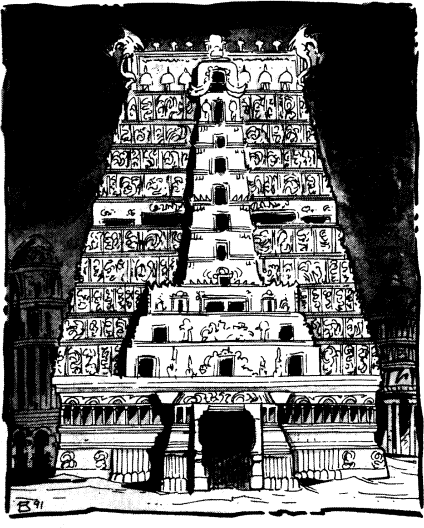
\includegraphics[width=\columnwidth]{images/tyr-1.png}
\par\textit{\small\textcopyright Wizards of the Coast, 2020.}
\end{figure}

\City{Tyr}
{15,000 (70\% humans, 10\% dwarves, 9\% half-giants, 6\% muls, 3\% elves, 1\% half-elves, 1\% other).}
{Iron, silk.}
{Common, Dwarven, Elven, Tyrian.}
{
	Located in a fertile valley in the foothills of the Ringing Mountains, it was the first city-state to successfully revolt against its sorcerer-king. King Kalak ruled Tyr until he fell to a group of heroes led by the gladiator Rikus, the wizard Sadira, and Agis of the noble house of Asticles. With Kalak dead, the High Templar Tithian stepped forward to take his place as king. Tithian received the backing of Rikus and the others, for the templar promised to free all Tyr slaves and institute other sweeping reforms---promises he actually kept. Tithian had his own agenda, of course, which slowly played out over the decade he held the throne.

	The new king created the Council of Advisers and gave members of the most important groups in Tyr a role in the city's government. Councilors were drawn from all ranks of society and worked diligently to pass laws that would strengthen Tyr's newfound freedom. Tithian allowed the Council to operate independently and virtually run the city while he sought the means to become a true sorcerer-king.

	Urik tried to capture Tyr's iron mines less than six months after Kalak's death. The resulting battles made Tyr's leaders realize how necessary a strong military was, and how important it was to resume iron production and get trade and commerce back on an even keel. During his reign, the new king also faced the problem of finding a way to overcome the Dragon's levy, had numerous skirmishes with raiding tribes, and battled angry giants intent on plundering the city. The Council struggled to stay together in the face of secret agendas and conflicting partisan interests. The templar revolt of Free Year 3 shut down the bureaucracy and public works for nearly two months until those who swore new oaths to abandon the old ways and support the tenets of Free Tyr were given more representation in the Council. The artisan strike of Free Year 6 lasted almost four months, and then ended in increased wages for basic services. Agis and the Council handled most of these crises in one way or another, for Tithian was much too busy to get involved in what he considered to be the chores of government.

	Today, in its twelfth year of freedom, Tyr faces new challenges. Agis of Asticles is dead, so his wisdom and honor can no longer guide the Council of Advisers. King Tithian's rule has come to an end. His ambitions led to his downfall, for he is trapped in the Cerulean Storm (though only a few people know of his true fate). The general populace believes that Tithian died fighting to keep Tyr free, thanks to the tales told by Rikus and Sadira. The heroes decided to keep Tithian's current state a secret, fearing that ambitious defilers might try to free him in order to gain power and prestige. Can Tyr's freedom take root in the Tablelands in the wake of these events, or will it be blown away in a devastating Tyr-storm?

	Tyr citizens remain as untroubled by modesty as they were in the days of Kalak. The less a person has to wear in the heat of the day, the better. Most wear loose-fitting cotton tunics gathered at the waist with wide, colorful belts. Others wear loincloths and vests. Light gauze or silks are draped over heads and exposed flesh to protect the skin from the blistering sun. Turbans and other forms of light headgear often finish off a Tyrian's attire.
}
{
	Four months into its twelfth year as a free city, Tyr must deal with the environmental and social conditions left over from the past decade. The Great Earthquake, for example, struck while most of Tyr's beloved heroes and its king were away. It fell to the remaining members of the Council of Advisers to pick up the pieces. Though the rumbling ground made for a terrifying period of time, Tyr escaped the disaster relatively unscathed. There was some structural damage and a small number of deaths, but most of these occurred in the Warrens. The comparatively weak and dilapidated buildings in this part of the city buckled when the quake hit, burying the residents beneath rubble and debris. Ironically, if the quake had struck during Kalak's reign, even less deaths would have occurred. In Kalak's day, the Warrens were mostly unoccupied. It's only since the First Edict freed the slaves that the Warrens have been filled to overflowing with the new crop of free citizens.

	The earthquake caused other damage. Cracks appeared in the city wall, and a whole section of the wall near the Grand Gate collapsed. Minor damage can be seen throughout the rest of the city, but the most noticeable appears on Kalak's Ziggurat. Great cracks riddle one face of the tower, while another face has collapsed into a heap of rubble. The client villages that dot the valley endured the worst of the quake's effects, however. One village was leveled by the quake, and others were pounded by rockslides that cascaded out of the mountains.

	Beyond the death and destruction, the worst aspect for the city is the refugees. Intelligent races and a wide variety of creatures and monsters have fled the mountains, flooding the valley in search of a safe haven. This, in turn, has sent villagers to the city gates, seeking protection from the ravaging hordes.

	What with the Great Earthquake, the periodic aftershocks that visit the city, and the violent Tyr-storms that occasionally sweep the land, the populace has turned into a frightened mob. Not everyone has succumbed to these base fears, of course, but a significant portion has lost control-the Council desperately needs to find a way to calm the people and restore order. A particularly vocal group claims that Kalak has returned to gain vengeance against the city, calling for open worship of the sorcerer-king to appease his wrath. Others have been trying to placate the elemental spirits of earth, hoping that they'll spare Tyr from their ground-shaking anger. Then there are those who seek to take advantage of the misfortune, looting shops, robbing nobles, and generally taking what they want and need by force of arms. These violent mobs are concentrated in the Warrens, but they sometimes range into other parts of the city to sow mayhem and destruction.

	The Council of Advisers has been working overtime to address these problems, though first it had to deal with King Tithian's supposed death. It established the OverCouncil to rule in Tithian's place so that the business of government could continue.

	Second, it increased the size of the City Guard and commanded it to restore order. Things haven't returned to normal yet, but the situation is much better than it was in the days immediately following the Great Earthquake. Various subcommittees have been set up to handle damage control, to see to the fair distribution of water and supplies, and to handle the refugee problem -both those rushing into the valley and those fleeing the villages for the safer environs of the city walls.

	The situations in the other city-states have added to the general nervousness and apprehension hanging over Tyr. While Urik has sealed itself off from the rest of the Tablelands (except for the heavily armed trade caravans that set out and return at random intervals), Gulg and Nibenay have made a few overtures to the Council of Advisers. Both city-states have offered to aid Tyr, claiming that without a sorcerer-king to defend it, the city is vulnerable to all sorts of terrible dangers. The Council, naturally, has thus far graciously refused these offers. Draj and Balic have recently resumed trade with Tyr, but both cities have changed significantly since the reported deaths of their sorcerer-kings. In fact, though Sadira and Rikus assured the Council that the kings had been disposed of by Rajaat, rumors of their return continue to drift in with caravans, adventurers, and refugees. The worst tales come out of Raam, where confusion, madness, and ambition have given rise to anarchy. Tales of nobles being murdered in their homes, of templars being slaughtered in the streets, and of vicious invaders from a hidden city-state controlled by a king named Dregoth have made the Tyr citizens ill at ease and not quite confident that their leaders can protect them.

	Sadira recently convinced a significant portion of the Veiled Alliance to come out of hiding and join Tyr society. These wizards formed a new group in Tyr, called the Preservers. The Preservers were given a place on the Council of Advisers to reflect their new role in Tyr. Sadira, as their leader and as an important member of the Council, was assigned to the OverCouncil. These good wizards are developing plans and guidelines for helping the city in a variety of ways that adhere to their overall morals and code of ethics.
}
{
\begin{figure*}[b!]
\centering
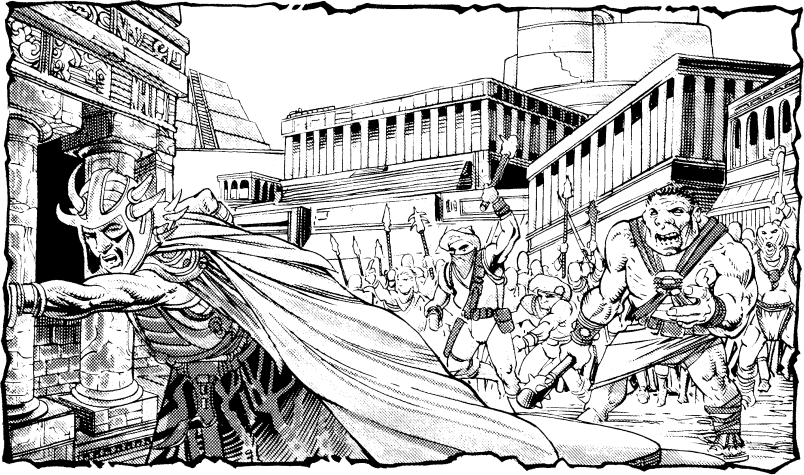
\includegraphics[width=\textwidth]{images/tyr-2.png}
\par\textit{\small\textcopyright Wizards of the Coast, 2020.}
\end{figure*}

	A Council of Advisers makes the laws of Tyr. The Council is divided into five distinct groups who together represent Tyr's varied citizenry. These groups are the Guildsmen, made up mostly of human and dwarf artisans and other professionals from Tyr's three trade districts; the Nobles, representing Tyr's aristocratic families; the Templars, who continue to handle administrative functions in the city; the Free Citizens, chosen from among the masses who were either slaves or paupers before Tyr's liberation; and the Preservers, the newest group admitted to the Council, consisting of members of the once secret and outlawed Veiled Alliance.

	When Rikus, Neeva, and Sadira returned with the news of Agis' and Tithian's death, it was resolved that the Free City shouldn't be burdened with another king. With no king to lead the city, the Council now oversees all aspects of government; a subcommittee made up of one member from each of the Council's divisions serves as an OverCouncil. This OverCouncil governs on a daily basis, while the entire Council of Advisers only meets three out of every fifteen days. The OverCouncil consists of the dwarf stonecutter Gar Bonehammer (NG male dwarf, expert 3) who represents the Guildsmen; Lady Laaj of Mycilen (LE female human, seer 6) for the Nobles; the High Templar Timor (LE male human, defiler 8) for the Templars; Rikus (NG male mul, gladiator 8/arena champion 10) who represents the Free Citizens; and Sadira (N female sun-touched half-elf, preserver 5/veiled one 5) for the Preservers.

	Surprisingly, the Council runs relatively smoothly. Some councilors posture for power and influence and partisan voting sometimes causes meetings to stall, but in general the Council has learned how to get the job done. Each division of the Council meets separately with its constituents to draft its own agenda before coming to a full session. Then the councilors do their best to get their own projects pushed through the voting process while trying to keep in mind the welfare of Tyr as a whole.

	While the Council deals with the big picture, the templars continue to fill the administrative roles they have long been associated with. Since the loss of their spellcasting abilities, it has become doubly important for this division to demonstrate why Tyr needs them. The tangled bureaucracy has been reformed, but it still exists.

	Without the templars to turn the massive wheels of government, Tyr's infrastructure would have collapsed long ago. High Templar Timor (who hides his status as a defiler) serves as the Minister of Tyr, overseeing the various Senior Templars who run departments like Fields, Finance, Public Works, Water, and Trade.
}
{
	\textbf{Free Wizards}: With preserver magic no longer outlawed in Tyr, Sadira convinced a number of preservers to come out of hiding and openly proclaim themselves to the city. As a group the free wizards are not a strong cohesive group. Individual free wizards pursue their own goals, whether in the political arena or merchant activities. Only the desire to instruct the populace in the differences between preserving and defiling magic and to build the public's trust in them unites the group.

	\textbf{House Vordon}: Under the last years of Kalak's reign, House Vordon had fallen from its position as one of the most powerful merchant houses in the Tablelands. Since the fall of Kalak, House Vordon has returned to a position of respect among its peers. The House's return to profitability is fueled by its specialization in the iron trade from the mines of Tyr.

	Thaxos Vordon is head of House Vordon. In the last ruinous days of Kalak's reign, Thaxos began a plan to overthrow the mad king. However, Kalak's demise at the hands of Rikus and the heroes of Tyr stopped him from going forward with the plan. In the years since, Thaxos has become convinced that he should become king of Tyr, and has refined the plan he originally developed for Kalak's overthrow. A number of dummy merchant houses have been created and large numbers of mercenaries hired as part of this plan. Unbeknownst to all but the highest members of House Vordon, Thaxos now has an army scattered at outposts throughout the region, waiting for his orders.

	\textbf{The Veiled Alliance}: The Veiled Alliance remains active in the wake of this new age of wizardly openness. Matthias Morthen (LG male human, preserver 8/veiled one 10) continues to lead a small number of preservers who feel that secrecy must be maintained until all of Kalak's defilers have been eradicated and the citizens of Tyr learn to deal with the responsibilities of freedom. Besides, Morthen doesn't like or trust Sadira, whom he believes has often approached the moral line between defiling and preserving magic (if not actually crossed over it) in the course of defending Tyr. He believes that the Veiled Alliance must continue, if only to serve as a balance for a wizard whose powers and motivations he doesn't fully understand.
}
{
	\textbf{Hidden Village (Thorp, 250)}: Established by the slave tribe known as the Free, the Hidden Village sits in a remote crater in the foothills of the Ringing Mountains between Tyr and Urik. Originally the tribe survived by raiding as most slave tribes do. Now the tribe has advanced into a small trading house. The villagers have developed such a strong relationship with Tyr that they have become a client village of the free city.

	\textbf{Kled (Village, 450)}: Kled is a Dwarven community that has ties to Tyr. Possibly the largest Dwarven community in the Tablelands, Kled was built near the ruins of the city of last Dwarven kings, Kemalok.

	\textbf{Mira's Halo (Thorp, 50)}: Mira's Halo is a merchant outpost owned by House Qual, one of House Vordon's dummy trading houses. The outpost is used in the iron trade between Tyr and Urik. The name of the outpost comes from an unusual rock formation nearby.
}
{
	\textbf{The Elven Market}: The Elven market is located inside the Warrens. Several nomadic Elven tribes trade at the market regularly, bringing a wide range of goods and curiosities from across the Tablelands. Many tribes own a building or two that borders on the square. Others take ownership of unoccupied buildings for the duration of their visit in Tyr. Anything can be found in the Elven market, legal or illegal. The customer just has to know the right people to ask. The market has a reputation for pick pockets and dubious merchandise, but people come from all over the city in order to find items not available anywhere else in Tyr.

	\textbf{Gladiator Stadium}: The Gladiator Arena of Tyr is the second largest building in the city, with only the ziggurat, which looms over one end of the stadium, being larger. The stadium's rectangular floor is some 90 meters long and 24 meters wide. The floor is of a hard packed sand with a reddish hue, which Tyrians say is caused by the spilling of the lifeblood of a thousand fallen gladiators. The stadium is unique in the Tyr Region as it has upper and lower seating sections. The upper section is generally referred to as ``The Sun Seats'' because of the lack of shade, and is open to the general populace. The crowd in the upper section is more raucous and enthusiastic than in the lower section. Seats in the lower section cost more and are traditionally used by merchants, and nobles.

	Despite the end of slavery in Tyr, gladiator matches are still held in the stadium. Now the bouts are not fought to the death and are open to any who wish to participate.

	The gladiator matches are only held on festival days. The remaining time, the arena floor is used for an open air market. A monthly array of tents and stalls cover the sandy floor in drunken rows. Traders who operate in these stalls offer a wide variety of legal and illegal goods and services.

	\textbf{Golden Tower}: The Golden Tower was the imperial home of the King of Tyr. Both King Kalak and King Tithian ruled from the Tower. Constructed of a rare golden granite, the tower gleams harshly during daylight. The only public entrance to the tower is to cross Tower Bridge from the Observation Tower. The public receiving areas are on the top floors, with the King's private chambers on the levels below. These included the King's library, an enormous collection of scrolls and books, many from ancient times.

	\textbf{Iron Mines}: Tyr's iron mines are the largest in the Tablelands and help the city exert leverage over the other cities in the region. The iron mines are located two days, travel northwest of the city. Death has always surrounded the mines, from cave-ins to the ``hej-kin's curse.'' The iron ore is transported to Tyr in heavily guarded caravans.

	\textbf{Kalak's Ziggurat}: The ziggurat built by Kalak still towers over the squalor of the city from its center. The ziggurat is a stepped pyramid with each level finished in a different colored glazed brick. An enormous staircase runs straight from the base to the summit of the ziggurat. Since Kalak's fall, the ziggurat has fallen into disrepair. The Great Earthquake has exacerbated this, causing an entire face of the pyramid to collapse. Great cracks riddle another face of the tower, causing concern that more of the pyramid may crumble soon. Few have dared enter the ziggurat since Kalak's death and it has become the focus of numerous rumors and frightening stories.

	\textbf{School of Thought}: The School of Thought is the only major organized institution for the study of psionics in Tyr. The school was founded a little over 30 years ago by the noblewoman Chessia. Chessia provided the funds to establish the school and made contributions to help the school operate over the years, but she is not involved running the school. The current headmistress of the School of Thought is Sycia Strimmen (NG female human, telepath 7/psiologist 9), a young and enthusiastic woman with considerable charm. She has been the headmistress for almost nine years now, since the previous headmaster, Thanik Arkos, disappeared from the school after murdering one of the master instructors. Sycia is very organized and well liked by students and instructors alike.

	\textbf{Shadow Square}: Shadow Square is a small entertainment district in the Warrens near Kalak's Ziggurat. Five lanes end at the small plaza around which sit six wineshops, a gambling house, and two hostelries. Most business in the square happens between sunset and dawn.

	\textbf{UnderTyr}: The site the city of Tyr was built on has been inhabited for thousands of years. The current city sits atop the ruins of these previous civilizations. An undercity of interconnecting byways, crumbled buildings, and dilapidated courtyards exists under the streets of modern Tyr. From buildings used as businesses to former residences and temples to forgotten gods all make up the structures of UnderTyr. It is not possible to travel from one side of the city to the other through UnderTyr. Instead pockets exist throughout the city. The location of the eight largest pockets is scattered and unconnected across the city. With names such as the Sorrows, Elven River, and Merchant's Maze, these underground locations provide opportunities for the brave or foolish. Many strange and wondrous items can be found in UnderTyr, as can dangerous creatures and malicious entities.

	\textbf{The Warrens}: The Warrens sprawl across the northern quarter of the city. The slum is filled with dilapidated structures and trash dumps. The district is filled to overflowing with the poor, mostly ex-slaves. Many are out of work, and the desperate and ambitious have chosen to prey on their neighbors. Gangs roam the Warrens targeting anyone who looks like they might have a ceramic piece. Templars and the city guard rarely patrol the Warrens anymore for fear of being overrun by the mob. Parts of the Warren are said to be cursed. Other buildings are said to be haunted or the lair of some wild beast. Anyone who enters the Warrens does so at their own peril.
}
{
	\item Slavery is outlawed in Tyr, but a group of slavers has set up a network to kidnap citizens of Tyr and sell them as slaves in other cities. The slaver network is elaborate, involving snatch teams that kidnap the victims, nobles whose estates are used to hold the captives, templars who look the other way, an Elven tribe that smuggles the slaves out of the city, and a merchant house, perhaps House Shom, that transports the captives to other cities where they are sold.
	\item Is the shadow of Kalak's ziggurat deadly? Rumors fly that ever since King Tithian's death, people are suddenly dropping dead while standing in the ziggurat's shadow. Those living close to the ziggurat are fearful of falling under what they have named Kalak's Curse. Many are fleeing, but no one knows what is causing the deaths.
	\item The elderly noblewoman Prisella Obstrunia is unlike many of her fellow nobles. Since the slaves were granted their freedom she has come to regret her past participation in the practice, and seeks to make amends somehow as she nears the end of her life. One of her former slaves, Raxenth, has remained with her as a servant and become a friend. When slavery was still in practice in Tyr, Prisella had sold off a number of Raxenth's relatives. Now, she wants to reunite Raxenth with these relatives, who through the slave trade have been scattered across the Tablelands. The noblewoman will hire the PCs to track down Raxenth's relatives and bring them back to Tyr.
	\item Zacraloc is the landlord for a large section of the Warrens, where most of the poor cannot afford to own their own homes but rent dilapidated buildings from Zacraloc. Seeking to increase his land holdings, Zacraloc uses hired thugs to set fire to a large section of the Warrens, which he does not own. His intentions are to approach the owners of those who lose their houses in the fire and offer to buy the ruined homes for very little money, since the desperate victims will need any money they can get. But the fire spreads out of control fed by either fire clerics or fire elemental creatures attracted to the original blaze.
	\item One of the rare, well-respected templars with no known enemies is found murdered. The templars are demanding better protection and seek to use the murder for political concessions by blaming the freemen. Freemen politicians reject the acquisitions but attempt to hinder the investigation, because they fear what would happen if the allegations were true. The truth is that it was not a political murder. The templar was murdered by a woman he sold into slavery years ago to merchants from Balic. The woman only recently escaped slavery during the confusion of the Wavir coup and returned to Tyr where she tracked down the person responsible for her enslavement.
	\item Tired of the raids by hej-kin on the iron mines, the Council of Advisors decides to send emissaries to the hej- kin to negotiate some sort of truce. Timor, the senior templar on the Council, does not believe the negotiations will be successful so before the PCs leave he secretly asks them to map out their journey to the hej-kin lair. With this map, a military expedition can be led to wipe out the hej- kin threat. To further complicate the PCs' mission, an agent of King Hamanu has infiltrated the mine as a guard and seeks to broker an agreement with the hej-kin on behalf of his master.
}
\begin{figure}[b!]
\centering
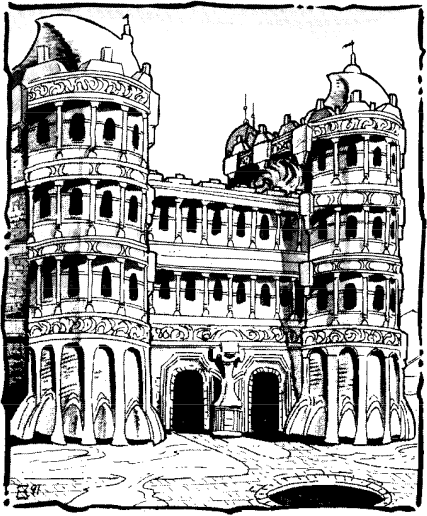
\includegraphics[width=\columnwidth]{images/urik-1.png}
\WOTC
\end{figure}

\City{Urik}
{30,000 (75\% humans, 10\% half-giants, 5\% dwarves, 3\% muls, 3\% thri-kreen, 2\% elves, 1\% halfling, 1\% other).}
{Obsidian, silk, pottery.}
{Common, Dwarven, Urikite.}
{
	Located northeast of Tyr, between the Dragon's Bowl and the Smoking Crown Mountains, the square, clean lines of the city-state of Urik can be found. The city-state has remained virtually the same as it was before the Great Earthquake and the demise of the Dragon. Hamanu, the King of the World and the Lion of Urik, was away from his city when the tremor struck.

	Although minor damage and only a few deaths resulted from the quake, the citizens trembled. When Hamanu returned, he promised his citizens that they would have nothing else to fear from Athas and its cruel temperament. The sorcerer-king's word (and his magic) was as strong as precious steel, for neither the aftershocks nor the Tyr-storm that arrived two months later could breach the towering yellow walls of Urik.

	Hamanu's promise wasn't unconditional. Though the Urikites don't have to fear change, they do have to fear their king. To disobey Hamanu is to risk punishment and even death, while to obey him is to live without fear. That's how it's always been in eternal Urik, and that's how it always will be.

	Urikites wear their hair in square cuts with elaborate ringlets. Some men wear square-cut curled beards. White linen shirts with short, tight sleeves are the fashion of Urik. Individuals of the lower classes wear plain, unadorned shirts that fall to their knees. Individuals of the upper classes increase the length to their ankles and add a striped or diamond pattern as well as a tassel-trimmed girdle. Elaborate scarves, worn only at night, indicate a citizen's station. The longer and richer the scarf, the higher the wearer's social status. By law and tradition, only templars may wear cloaks, and these are always bleached pure white for the low to mid levels and tinged yellow for the higher ranks.
}
{
	Except for the new restrictions regarding trade and travel, things in Urik are the same as they ever were. The city remains a warrior culture, ruled by a warrior king and geared toward fighting and winning wars. The current enemies aren't the other city-states, however. Rather, the refugees seeking shelter from the constant tremors and the monsters fleeing from the violent storms near the Silt Sea have become Urik's foes. When either approaches Urik's high, yellow walls, Hamanu leads his army out of his gigantic palace (called Destiny's Kingdom) and charges into battle. In most cases, the result is slaughter, for terrified invaders can't stand against Hamanu's highly trained and well-equipped legions.

	The few signs that the Great Earthquake touched Urik have been wiped out; buildings have been repaired, streets repaved, the dead buried. Now, Hamanu's magic keeps the aftershocks and the storms from entering the city, and in most respects the citizens have learned to ignore the disasters. As long as the disasters remain outside Urik's walls, the citizens see no reason to worry about them.

	Closing the city off from the rest of the world has made it difficult for certain members of Urik's society. Adventurers and traders, for example, are severely hampered by the well-guarded walls. Elves, never really welcome near Urik's walls, now avoid the city completely. They are treated like invaders, set upon as soon as they're spotted entering Urik's verdant belt. Things may change as soon as the king finishes contemplating his city's new approach to the world---or it may simply get worse if Hamanu decides to keep the rest of Athas at bay forever.
}
{
\begin{figure*}[b!]
\centering
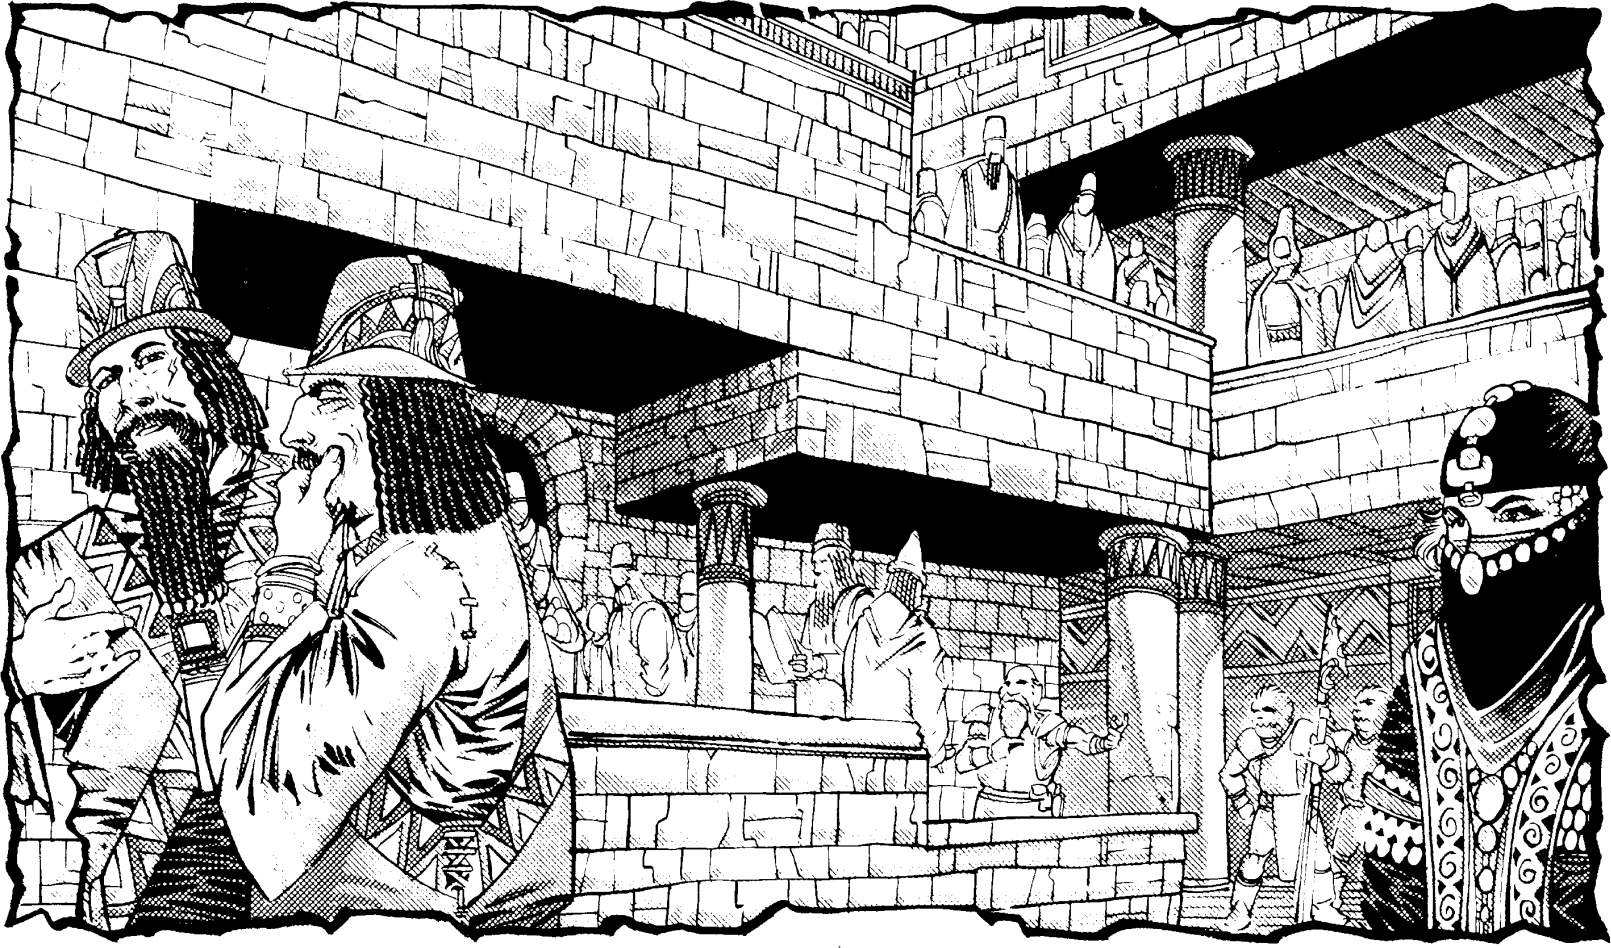
\includegraphics[width=\textwidth]{images/urik-2.png}
\WOTC
\end{figure*}

	The sorcerer-king Hamanu rules Urik, taking a personal interest in the affairs of his city. Except for Hamanu's direct involvement, Urik operates as a traditional sorcerer-king's domain. Templars enforce Hamanu's laws and handle the day-to-day bureaucracy, nobles manage the farms and water supplies, free citizens engage in business and try to remain free, and slaves provide the muscle to get everything else done.

	Hamanu is a third-stage dragon king (LE male Champion of Rajaat stage III dragon, defiler 5/psychic warrior 11/arch defiler 10/cerebremancer 5/Athasian dragon 4). Through a combination of the Way and magic, he appears before his subjects as either a tall, vigorous man with close-cropped silver hair, dark skin stretched tight over ruthless features, and heartless yellow eyes, or as a half-man and half-lion of powerful build and mythic proportions. He is never seen in his true dragon form, even by his most-trusted templars. His laws, called Hamanu's Code, are strict and innumerable, covering almost every conceivable aspect of life in Urik. Hamanu's Code relies on punishment in kind and emphasizes loyalty to the king and his templars. The Code stands unsurpassed in the Tyr Region for utility, comprehensiveness, and ruthlessness.

	At one time, Hamanu's ambitions exceeded his resources. Since the Great Earthquake and the events surrounding Rajaat's brief return, his agenda has subtly changed. The three surviving sorcerer-kings sensed that the time had come to rethink the old ways, to find new approaches to the challenges of life on Athas. Until he figures out what those new approaches are, Hamanu has decided to withdraw a bit. He has effectively closed Urik off from the rest of the Tablelands, trying to keep change from intruding on his domain for as long as possible.
}
{
	\textbf{The Brotherhood of the Mind}: The Brotherhood of the Mind is an organization of evil psionic-users that wish to overthrow the sorcerer-kings and seize power for themselves. Ruled by Liumakh, an undead psion, (NE male undead, telepath 10/thrallherd 7) the Brotherhood is headquartered in a monastery in the Smoking Crown mountains. Both Hamanu and Nibenay know of the brotherhood's existence. Nibenay seeks their destruction, while Hamanu ignores them for the most part, though he occasionally spies on the brotherhood to see if they have developed anything interesting during their psionic studies.

	\textbf{Hamanu's Halflings}: Hamanu has forged an agreement with a halfling chief from the Ringing Mountains. As long as Hamanu provides the chief with obsidian from the Urikite mines, he receives the services of 200 halfling warriors. These halflings are excellent night raiders and assassins that Hamanu has used to deadly effect in the past.

	\textbf{House Stel}: House Stel is best known for trading in the spoils of war, weapons, slaves, and various stolen cargo. Heavily influenced by the militant nature of Hamanu's regime in Urik, Stel is aggressive and confrontational with rivals. Stel caravans are heavily guarded to prevent against raids from other merchant houses, a tactic the house uses on its rivals regularly. The leaders of House Stel have a deep hatred of elves which has led to open warfare with a number of Elven tribes over the years. The House maintains lucrative trading contacts with halflings of the Ringing Mountains. Hargan Stel III (LN male human, fighter 5/rogue 2/ dune trader 5) leads the house and reflects the nature of his house, being both an expert trader and warrior.

	\textbf{The Veiled Alliance}: The Veiled Alliance has to be doubly careful in the wake of Hamanu's restrictions, and the preservers' supplies of spell components have become extremely limited. For most of the decade following the war with Tyr, Urik's Veiled Alliance was split into two factions. Its leader, the legendary Morlak, disappeared mysteriously, leaving two preservers to contend for the spot he vacated.

	When one of the contenders, Leoricius the Untamable, was killed in the Great Earthquake, the other contender worked feverishly to heal the split. This became increasingly important in the wake of Hamanu's newest restrictions. Today, Thania (LN female half-elf, preserver 5/veiled one 7) commands a whole Alliance, advocating patience and negotiation instead of the violent confrontations advocated by her one-time rival. Thania has been working to establish a partnership with Tyr's Alliance, but if Hamanu learns of it both groups will undoubtedly suffer.
}
{
	\textbf{Makla (Village, 1,000)}: The obsidian mines of Urik are located on the Mountain of the Black Crown, a peak in the Smoking Crown mountain chain. Urik's economy is completely dependent on obsidian and the tools fashioned from it. The Urikite client village of Makla serves as a base camp for the mining operations on Black Crown. The village is located on the shores of the Lake of Golden Dreams. Heavily fortified with over 500 guards, it is rarely attacked by raiders.

	\textbf{Fort Courage}: Fort Courage is a massive fortress on the trade road between Makla and Urik. This facility of House Stel is a supply point for caravans traveling between Urik and Makla and the halfling village of Ogo. Patrols are also sent from the fort to discourage raids on caravans along this route.
}
{
	\textbf{Destiny's Kingdom}: Sorcerer-King Hamanu rules Urik from his palace inside the massive fortress of Destiny's Kingdom. The walled fortress covers one square mile at the center of the city, containing troop barracks, drill fields, and an armory to support the army, as well as administrative offices for the king's templars.

	\textbf{The King's Academy}: The only legal psionic school in Urik is located within Destiny's Kingdom and is called the King's Academy. Students who attend the Academy are subject to a strict education that brings harsh punishment for failure. At the same time students are indoctrinated with the militarism that runs through the government of Urik.

	\textbf{Little Jungle}: A portion of the drill fields inside Destiny's Kingdom has been set aside for Hamanu's halfling allies to make their homes. Little Jungle is the name given to the fenced off area, where the halflings build huts in the jungle style.

	\textbf{Pit of Black Death}: Urik uses the site of an old obsidian mine for a gladiator arena, thus giving the arena its name, the Pit of Black Death. The Pit does not rise above the ground but is sunken into the ground. Stepped excavation provides viewing platforms for the crowd. All spectators must stand in the Pit, as there are no seats in the arena. The irregularly shaped combat area is made entirely of obsidian. The sun heats the black obsidian until it becomes almost unbearable for both combatants and spectators. As such most gladiator matches are held in the morning before the heat has become too great, or on rare occasions at night. Another danger of the obsidian is the thousands of sharp edges, shards, and spikes that protrude from the walls of the arena. These obsidian shards cover the walls and columns of obsidian that are scattered around the arena floor.

	\textbf{Potter's Court}: Pottery is an art form in Urik, and all other city-states recognize the superiority of Urikite pottery. The potters' workshops are collected in the Potter's Court area of the city. The concentration of so many immense kilns in the area, make Potter's Court unbearably warm, even at night when most of the potters conduct their work.

	\textbf{Potters' School}: The Potters' School is the largest group of psionic users who refuse to attend the King's Academy or register with the authorities. While the Potters' School teaches pottery casting and painting, skilled psions instruct students in the Way, outside of the influence of King Hamanu and his templars. The head instructor of the psions is Erriok (LN male human, shaper 7). He is rumored to have contact with the Veiled Alliance and work with them on occasion.

	\textbf{Three Sisters Observatory}: The Three Sisters Observatory is a two storey building with a flat roof and many observation balconies built on top of a hill called Sunrise Point. The Three Sisters Observatory served as the king's observatory until the construction of the Royal Observatory. Now the building is used to store old astronomical records and equipment, and has a run down, neglected appearance. The observatory gets its name from three identical granite hills nearby.
}
{
	\item Templars arrive at where the PCs are staying with orders to arrest them. Someone has accused the PCs of practicing magic. A fair trial is not possible and the sentence is death. The PCs must escape the templars, find out who their accuser is, and clear their name before they are captured by the templars.
	\item Unbeknownst to the PCs, their names have been added to a bounty list the templars of Urik maintain. Templars and bounty hunters begin to appear, trying to collect the bounty by capturing or killing the PCs. Whether or not the PCs are wanted by the templars, in this instance it is a case of mistaken identity. A wealthy merchant, wanted for smuggling, is supposed to be on the bounty list, however, he bribed a templar to remove his name and that of his family from the list. The PCs' names were chosen at random and added in place of the merchant's and his family to fill the vacancy.
	\item House Wavir has heard rumors that King Hamanu is planning on ordering his templars to seize all of their house's assets in Urik. Using the Wavir coup in Balic as an example, the house will be accused of planning a rebellion in Urik. Before he goes through with this threat, Hamanu is checking with the other major merchant-houses to gain their acceptance of his actions so they do not boycott his city. House Wavir gets wind of the plot and secretly plans to sneak out of the city with as much of their assets as possible. The PCs are hired to coordinate and have to safely get the Wavir agents and as much of their various assets, including wagons, merchandise, and draft animals, out of the city.
	\item The PCs are attending a feast at a noble's compound when the head of the family is murdered. Templars descend on the compound preventing anyone from leaving. Instead of investigating the crime, the templars simply state that unless the murderer is presented to them by morning everyone in the house will be executed. The PCs have until morning to find the real killer, or be executed along with everyone else.
	\item The Veiled Alliance has wondered for years about the high drik transformation process. The PCs are assigned to steal a drik egg that has undergone the process but that has not yet hatched.
	\item Saita, a templar of Urik, secretly sold some of the city's slaves to a tribe of yuan-ti in the Ringing Mountains to make some extra money. Unfortunately, the slaves were the personal property of Hamanu who is now enraged that his slaves are missing, and wants the head of the person responsible. Saita is desperate to get the slaves back before it is discovered that she is the one responsible. She secretly hires the PCs to get the slaves back from the yuan-ti any way they can.
}
\section{Beyond the Tablelands}
Plenty of action and adventure can be found across Athas. More lands of wonder, mystery, and danger exist beyond the barrenness of the Tablelands. A quick tour of these other places follows, and more information about specific locations will be revealed in future products.

\SubCity{Eldaarich}
{21,000 (85\% humans, 8\% dwarves, 4\% half-giants, 2\% muls, 1\% others).}
{Gold, silver.}
{Eldaarish, picts.}
{
\Figure*[\textwidth-2cm]{b}{images/city-eldaarich-1.png}

	Eldaarich occupies a small island in the Sea of Silt, just off the mainland. Here, isolated and protected from the rest of Athas, the citizens huddle in the paranoid delusions of their mad sorcerer-king. Daskinor, ruler of Eldaarich, believes that unknowable forces in the world are trying to destroy him.

	Every few years he puts a new name to these forces---the Order, the Veiled Alliance, Rajaat, pyreen, a merchant house, a lowly slave, or some other identifiable target becomes the imagined source of his fears for a time. Daskinor does his best to destroy these imagined enemies, and anyone who has even a passing resemblance to the target is persecuted until the next delusion grips him.

	Daskinor was never a stable ruler. From the beginning of his reign as sorcerer-king of Eldaarich, he was tormented by unfounded fears and nameless terrors that preyed upon his mind. For the first few centuries of his reign, he was able to function more or less normally despite his growing paranoia. As time passed, genuine bouts of panic began to intrude upon his psyche. These bouts lasted longer and longer, paralyzing Daskinor for hours, days, sometimes even months at a time.

	Eldaarich was constructed to protect Daskinor from his fears. Fortified walls, a strong military, devoted templars, retractable bridges, and a series of keeps and forts ensured that the entire city-state and surrounding area was secured against outsiders. Over time, it became less of a fort and more of a prison, locking king and citizens alike behind sturdy gates and high walls. Seven centuries ago, the sorcerer-king's paranoia became acute. He completely sealed his city, cutting off all ties to the other city-states. That was the way things remained until about FY 0 year, when limited trade was resumed with House Azeth of Kurn.

	Today, Eldaarich remains an isolated prison of a city. Daskinor's fears have become the fears of his citizenry, making everyone who lives under his rule as paranoid as he is. No one ever leaves Eldaarich, and no one ever enters its massive gates. It's a closed society---figuratively and literally.
}
{
	Every outsider wants to destroy their city-state and their sorcerer-king, and everyone who lives within the walls waits for an opportunity to betray you. That's what the people of Eldaarich believe, for that's what their leaders believe. Nowhere else in all of Athas is there such an underlying current of genuine, unattributable fear. It filters down from Daskinor himself, making citizen and slave alike tremble with uncontrollable paranoia.

	The citizenry is a subdued, cowering lot, given to unexpected bursts of violence once the fear inside them becomes too much to contain. In many cases, the ever-crushing weight of terror and oppression keeps the masses down, but sometimes a delusional artisan will strike out at a templar or noble, causing the level of paranoia to rise even higher.

	The quality of life isn't good in Eldaarich. Because Daskinor doesn't trust anyone, he allows his templars to dispense only the barest essentials to the free citizens and slaves. With just enough food and water to sustain them and few personal possessions, the people of the city are a sad, pathetic lot. They have no hope of a better life and no concept that a better life exists outside the walls of Eldaarich. If anyone even suggests such a notion, the ingrained fear of the unknown kicks in and makes everyone else dismiss the idea.

	While the class structure of noble, free citizen and slave exists in Eldaarich, the truth is that everyone beneath the templars is a slave to Daskinor's all-pervasive fear.

	The sorcerer-king sees threats to his rule on every face and in every dark shadow. For this reason, he permits no freedoms of any sort, not even the token rights given to the citizens of other cities. Freedom, Daskinor believes, is just an opportunity to betray his trust. So he orders his templars to oppress the people of his city, to make their lives so miserable they don't have time or strength to contemplate treachery.

	The templars don't have it much better. They're kept in line by the high templars who, in turn, are subject to Daskinor's brutal whims.

	The majority of the population consists of humans, though there are also dwarves, half-giants, and muls in significant numbers. There are also a few aarakocra wasting away in the slave pens. Daskinor has a particular hatred of the winged people and gives his templars special compensations for capturing aarakocra from the nearby White Mountains.

	If travelers were to find themselves in Eldaarich or one of its holdings (which isn't very likely), they'd feel the weight of oppression and smell the stench of mental illness that hangs in the hot, stifling air. Every year the darkness in Daskinor's soul grows deeper, his paranoia more acute. This mental deterioration is reflected in the city itself, as though each citizen were a part of the sorcerer-king's diseased mind.
}
{
	The same model of government evident in the other city-states exists in Eldaarich. The sorcerer-king Daskinor (CE male stage II Champion of Rajaat dragon defiler 8/nomad 10/cerebremancer 10/Athasian dragon 2) stands atop the societal hierarchy, his troubled delusions coloring every aspect of life in the city-state. His chaotic tendencies and often overwhelming paranoia infuse everyone he comes in contact with, making the city almost as wild and frenzied as Raam. The only thing that allows the city to function is that the citizens are a subdued lot, living in quiet fear instead of in rambunctious anarchy. Daskinor constantly watches over his shoulder for assassins that don't exist, and so do his templars and nobles. No one trusts anyone else in Eldaarich. This works out for the best, as the troubled atmosphere has fostered a society where the fear of murder and betrayal has encouraged the periodic use of such techniques by those who prefer to strike first.

	Templars and nobles regularly kill each other to keep the same from happening to them, or to gain power or position, or just because the tension of living behind heavy locks and being constantly on guard eventually drives even the most peaceful beings to violence. In Eldaarich, fears permeates everything---fear of the sorcerer-king, fear of outsiders, fear of each other, and fear of the unknown. Because the society is closed off to the rest of the world, everything on the other side of its walls and locked gates is, by definition, unknown.

	If Eldaarich is a prison, Daskinor is its most prominent prisoner. The sorcerer-king lives in a walled sub-city and rarely ventures into other parts of his realm. His constant paranoia sometimes intensifies to such a fevered pitch that he ceases to function.

	In such a state, which may last as long as months at a time, Daskinor is cared for by his senior templars. At other times, his paranoia drives him to give a name to his fear. When this occurs, the entire city mobilizes to combat this supposed threat to the realm. Currently, the use of psionic abilities has been outlawed, as Daskinor believes that the Order has initiated a campaign against his rule. Even low-powered psionicists and wild talents who openly display their abilities are subject to imprisonment or death because of the current edict. Only Daskinor, a psionicist of the highest caliber, is exempt from the terms of the edict.

	Daskinor's templars serve as administrators to the city, and also act as the sorcerer-king's eyes and ears in all corners of the domain. They are charged with watching for signs of treachery among the masses-and with dealing with such treachery before it gets out of hand. The templars are as paranoid and delusional as Daskinor, giving in to their fear whenever it overwhelms them. For this reason, Eldaarich has become a police state, and the templars are the police. They command the military. They oversee all records and the distribution of goods and services. They hold the power of life and death for the rest of the citizenry in their terrified hands.
}
{
	\textbf{Kulag:} The Kulag Order controls Daskinor's silt fleet, which currently acts as the merchant house for the Dim Lands, a nearby archipelago. It is leaded by High Templar Kerillis (LE female human, templar 14). Sometimes they also resort to piracy in the nearby islands.

	\textbf{Neshtap:} More commonly known as ``red guards'', the Neshtap are the most feared, and the second-most powerful of seven orders that Daskinor uses to maintain control of his city Eldaarich, and its client villages. They never speak, seemingly revere the element of fire, and are becoming increasingly powerful and independent from Daskinor.

	\textbf{The Veiled Alliance:} Eldaarich has no Veiled Alliance. Daskinor rooted out the Alliance and destroyed it 400 years ago when the group of preservers became his imagined enemy of the moment. Some preservers still live in the city, but they remain hidden and are relatively weak due to a lack of adequate training. Preservers from Kurn sometimes sneak into the closed city to provide training and to see what the conditions are, but they don't do this very often. If they get caught, they're put to death, and if their city of origin is discovered, it could mean war between the two cities. No one, especially Oronis the Avangion of Kurn, wants a war to break out. He does, however, feel the pain that both Daskinor and his citizens project, and often contemplates finding a solution to Eldaarich's problems.
}
{}{}
{
	\item A silt schooner owned by House M'ke was attacked and captured by the navy of Eldaarich. The merchant house could hire the PCs to raid the harbor of Eldaarich and bring the schooner back.
	\item An aarakocra from Winter Nest was captured when she flew too close to Eldaarich. The PCs are asked to free her before she is executed by the templars of Eldaarich. Once freed from her cage, the aarakocra can easily fly back to Winter Nest on her own, but the PCs will have to sneak out of Eldaarich.
	\item Grehgatha is a Kurnan preserver who has snuck into Eldaarich many times to tutor young preservers. Since she has returned from her last attempt she is consumed with freeing an entire village from Daskinor and hires the PCs to help. The PCs must come up with a way to sneak 150 people past the templars of Eldaarich.
	\item The Red Guard has become jealous of the monopoly on trade held by the templars of the Kulag Order. In an attempt to disrupt the trade negotiations, the Red Guard mounts a surprise attack on Silt Side during a meeting between Corik Azeth and High Templar Kerillis. The PCs acting as guards for House Azeth may misinterpret the attack as directed by Corik or themselves.
	\item Concerned with a recent rise in the level of the silt sea around Eldaarich, the city has declared war on all silt clerics. Mercenaries are to be hired to help hunt down the silt clerics along the coast for a hundred miles north and south of Eldaarich. The PCs could become embroiled on either side.
	\item A major giant raid on the Huuros Islands has been repulsed by the Kulag Fleet, though many casualties were suffered. Templars assign the PCs to salvage what they can from the battle, equipment as well as the bodies of those who died. Most of the wreckage is just off shore in silt 4.5 to 6 meters deep.
}


\SubCity{Kurn}
{18.000 (65\% humans, 10\% elves, 6\% muls, 6\% aarakocra, 5\% dwarves, 4\% half-elves, 3\% half-giants, 1\% other).}
{livestock, magic items, medicines.}
{Elven, Kurnan.}
{
\Figure*[\textwidth-2cm]{b}{images/kurn-1.png}
	Kurn is actually two city-states: an ancient, public metropolis, and a utopian city hidden from the rest of the world. Old Kurn sits in a lush meadow on the eastern side of the White Mountains. The trade road running north out of Draj connects Kurn to the Tyr Region, and the city welcomes merchants from the south. New Kurn lies in a fertile valley hidden among the White Mountains themselves. A secluded road protected by a towering fortress keeps the valley safe from unwanted visitors---and New Kurn doesn't want any visitors.

	Old Kurn was a prosperous but relatively small city from the Green Age that suffered great devastation in the early days of the Cleansing Wars. Once situated in a vast forest that has long since faded from the landscape, the elf city of Kurn was destroyed by the Champion called Albeorn, Slayer of Elves. When the Champions finally turned against Rajaat and became the dragon kings, the one named Keltis decided to build his city-state on the ruins of Old Kurn. He changed his name to Oronis, but decided to retain the name of the city he was building over.

	The ruins weren't in as bad a shape as Oronis originally thought. He was able to build upon many of the foundations, and a few whole structures were still fit for use. Within a decade, Oronis' Kurn was established. Within five decades, it was thriving. For five hundred years, Kurn followed the same course as the other sorcerer-king domains. Throughout that time, Oronis was troubled by something few of his peers possessed---his conscience.

	When he was Keltis, Lizard Man Executioner, he succeeded at the task Rajaat handed to him. He eliminated the entire race from the face of Athas. As the years passed and Keltis the Champion became Oronis the sorcerer-king, images of the atrocities he committed started to haunt him. After Oronis advanced to a second stage dragon king, his problems intensified. Now he had the deaths of his subjects on his head, for he had to use a specified amount of life force to power his transformation.

	He decided that none of this was what Rajaat originally promised him. Where was the restoration of the world? Athas hadn't gotten better because of the Cleansing Wars. It had gotten worse. What's more, the sorcerer-kings were continuing the downward spiral, slowly killing the world by their actions. Oronis refused to be a part of that trend any longer. He renounced his defiling skills and his status as a dragon king and sought a different path.

	That was when Kurn broke off relations with the other city-states. Mercantile activities continued, of course, but at a reduced rate. After a time, Kurn became one of the forgotten cities---just as Oronis had hoped. In the meantime, he set the next part of his plan for redemption in motion. Oronis wanted to make amends for the horrors of his past.

	The first step was to change the rules of society in Kurn. Though the city had to maintain an illusion of normalcy to keep the other sorcerer-kings from detecting treachery or weakness, Oronis secretly freed all slaves and instituted fair and just practices at all levels of society. He swore his citizens to secrecy, for if word got out he was sure his one-time peers would flock to Kurn like gith to a dying braxat. The second step was to begin construction on the utopia he envisioned. Like all ex-Champions, Oronis originally wanted to return Athas to the glory of the Blue Age.

	He decided to once more strive for that goal. In a hidden valley among the peaks of the White Mountains, the foundation stones of New Kurn were laid. As his templars and citizens worked to build New Kurn, Oronis went in search of a better path to power. Using the techniques and practices of preserving magic, Oronis looked for a way to combine magic with psionics in a more positive way than through dragon magic. It took nearly 1,000 years of study and experimentation for Oronis to develop the preserver metamorphosis spell. With it, the reformed sorcerer-king could become an advanced being aligned to goodness instead of another force for evil.

	Today, the twin cities of Kurn continue along their parallel courses. Old Kurn displays a typical sorcerer-king's domain to the other inhabitants of the region, at least on the surface, while New Kurn works to complete Oronis' experiment in regressing a small portion of Athas back through time. Between the two cities, Kurn has a total population of 18,000 people. The majority live in the new city, as each year more citizens are moved from the old city to the new. Old Kurn has such a small number of residents that it appears to be almost a ghost town, and one day Oronis plans to completely abandon it in favor of his secluded valley.
}
{
	The state of life in Kurn depends on which of the twin cities is being considered. Old Kurn, on the surface, appears to be much like any city in the Tyr Region still ruled by a sorcerer-king. Surface appearances, however, can be deceiving. Travelers who stay for any length of time might notice a few oddities. For example, the slaves seem to have a sparkle in their eyes and a bounce in their step that isn't seen in the other city-states, and templars aren't given as wide a berth as their counterparts in Urik or Nibenay. Additionally, while the merchant and tradesmen districts are always crowded, the rest of the city is as empty and desolate as the ruins of Giustenal.

	Old Kurn maintains its illusion of business-as-usual through the cooperation of its citizens and the advanced powers of its sorcerer-king. If visitors notice that the noble and templar quarters of the city are practically deserted, they usually attribute it to the rumors that Kurn is slowly dying. Dying or not, the city is far from defenseless. More than one raiding tribe has attempted to take advantage of the ``dying'' city only to discover that its defenders were more than capable of driving them off.

	Through the efforts of House Azeth and the commerce provided by other traders, Kurn maintains a modest economy. While most of the inhabitants of the Tyr Region have forgotten that this northern city exists, Kurn interacts with its closest neighbors on a regular basis. It has good relations with the aarakocra of Winter Nest, the merchants of Draj's House Tsalaxa, and the elves of a few of the local tribes. Except for the contact between House Azeth and the trade templars of Eldaarich, Kurn has little interaction with its neighboring city-state. On the other hand, Kurn sometimes has trouble with raiders from the Bandit States. The raiders don't come to the gates of the city (at least not very often), but they do attack travelers on the trade road and even plunder the client villages on rare occasions.

	New Kurn is a different matter. The high, sturdy walls of Fort Protector block the eastern entrance to the hidden valley, while the tall, steep peaks of the White Mountains make the other directions inaccessible. The only approach that might be open is by air, though flying creatures loyal to Oronis nest in the vertical peaks.

	Within the valley, Oronis' restoration project is in full swing. He has turned the valley into a place from the past, recreating the conditions of the Green Age in its sheltered space. A thick forest surrounds a lush clearing where the city of New Kurn has been built beside a small, clean lake. Oronis hopes to eventually regress the valley to conditions as they were in the Blue Age, but that's still many years away.

	The new city resembles Oronis' vision of utopia. Airy buildings with tall, elegant spires grace wide, open streets paved with white stone. Here, the people govern themselves through a system of fair laws and majority rule. Everyone has a say in the workings of the city, from the poorest laborer to the highest elected official. And if someone doesn't like the way things are going, they're free to run for a position when the current terms of office expire.

	Thanks to the fertile valley and the lush forest, no one goes hungry or thirsty in New Kurn. No creatures are hunted out of existence and no plants are plucked completely from a given area. The templars monitor the forest on a daily basis to make sure the delicate balance is maintained. For this reason, no defilers are permitted within the ranks of the templars or anywhere in the twin cities. It is strictly against the laws of Kurn to practice defiling magic.

	Oronis continues to advance as an avangion, and he tries to instill the same serene, peaceful, life-giving properties of his new form in the city and people who follow him. Where once there was a man of evil, now Oronis is a force for good in the world. His templars work to promote his plans and prepare to someday strike out from the valley with the knowledge of how to restore all of Athas. Until then, they'll work to finish the restoration of the valley and to perfect the society that Oronis has inspired.
}
{
	Oronis the Avangion (LG male Champion of Rajaat stage IV avangion, preserver 5/shaper 5/cerebremancer 10/loremaster 3/avangion 5) guides the paths of the twin cities. Oronis spent centuries redeeming himself, going so far as to change his very nature from evil to good, though he still feels he has a long way to go to make up for his acts as a Champion of Rajaat and a sorcerer-king. For this reason, he has dedicated himself and his citizens to working toward the eventual restoration of all Athas.

	While in Old Kurn, Oronis wears the guise of a normal human. In this psionically and magically induced disguise, he appears as a tall, lanky, middle-aged man with short golden hair, pale-blue eyes, and a close-cropped blond beard. He covers himself in the trappings of a sorcerer-king, wearing a golden circlet on the crown of his head and carrying an obsidian-topped walking staff. In New Kurn, however, such disguises aren't called for. There he openly displays his true avangion form---a tall, thin, hairless humanoid with golden skin, silver eyes, and gossamer wings.

	Though Old Kurn appears to run like any other city-state, Oronis long ago abandoned a monarchical form of government. He allows his subjects to govern themselves via a democratic system he developed. In this system, nobles and all citizens except templars may hold public office. Elections are held at regular intervals and term limits are set. The highest elected official is called the Presider, who sits at the head of a body called the Tribunal. Members of the Tribunal are referred to as Tribunes. Together, the Presider and the Tribunes draft the laws that keep the city-state running smoothly. The current Presider is Ulali of Prusicles (LG female half-elf, preserver 8), now in the second year of a five-year term.

	Oronis refuses to hold an official position, though he does pretend to be sorcerer-king in the old city. He acts as an adviser when the Presider or Tribunal requests his presence, but otherwise, he's more concerned with advancing as an avangion and keeping the valley restoration project on track. Oronis' templars don't serve as administrators in Kurn, either. Instead, they are the keepers and dispensers of knowledge, serving as teachers and advisers to local officials and businesses. It's also their job to oversee and handle the restoration process, under Oronis' supervision.
}
{
	\textbf{Black Brethren:} Oronis' Black Brethren are Kurn's elite army, charged with patrolling Kurn and making sure Kurn is safe and secret.

	\textbf{School of Spies:} Kurn's School of Spies is an organization of Kurnan spies, mostly female, that studies non-Kurnan societies, and brings back information to defend Kurn and improve its way of life. They have managed to infiltrate into Merchant Houses and even the templarate of every city-state in the Tablelands.

	\textbf{The Veiled Alliance:} Kurn has no Veiled Alliance. Preservers are a welcome and significant part of the society, so there's no reason for them to hide behind a veil of secrecy. In fact, preservers from other Alliance factions sometimes come to Kurn to study with Oronis. One preserver, Korgunard of Urik, even learned the steps to become an avangion and followed the path forged by Oronis. It's conceivable that more avangions will appear in the future, though when and how many is hard to say. While preservers are accepted and integral to Kurn society, defilers are considered enemies of everything Oronis stands for. The avangion is reluctant to allow his followers to make defiling magic punishable by death, as he himself was once a defiler of the highest order. However, he knows that in most cases defilers can't make the mental and spiritual changes necessary to reject that path, so he has agreed that known defilers must be banished from the society.
}
{
	\textbf{Azeth's Rest (Village, 900):} This fortified oasis and trade village lies on the trade road, reaching north from Draj to Kurn. It has remained in the hands of House Azeth ever since the trade village was founded. Fifty tough mercenaries protect it and the nearby road, manning the ballistae and fixed crossbows atop its great walls. Azeth's Rest welcomes all traders, provided they can pay the fees for using its services.

	\textbf{Silt Side (village, varies):} Silt Side is an open village on the coast of the Silt Sea. Silt Side handles trade with Eldaarich; in fact, this village is the only connection with the outside world that Eldaarich maintains. Silt Side is a seasonal village, populating and emptying for a few weeks three times every year when House Azeth members meet to trade.
}
{}
{
	\item Oronis needs many unusual spell components for his studies. Often times he does not have the time to gather all of them himself, so he hires the PCs to collect some of the rarer spell components he needs, such as roc eggshells, leather from a dune reaper matron, the bark of a zhackal, or silt eel tongues.
	\item The last time the PCs were in Kurn, they were befriended by Aloth, a friendly merchant. But now that they have returned to Kurn, Aloth has disappeared and his shop is being used by another merchant. No one claims to have heard of Aloth when the PCs ask. Has Aloth been secretly granted citizenship in New Kurn, or has something more sinister happened to him?
	\item The residents of New Kurn are up in arms when a patch of defiled ground is discovered. Suspicion falls quickly on the newest members of the community, the PCs. Actually, there is no defiler in New Kurn. The defiled ground was caused by a magical object that uses a defiling effect to power its magic. One of the preservers of New Kurn recently acquired the item and tested it, not realizing what it would do. Now he is horrified that he will be blamed for the defilement, anger Oronis, and be forbidden to practice magic, so he remains silent.
	\item The PCs have to figure out who murdered a merchant in Kurn. But the investigation is hampered when many of the witnesses and suspects disappear. Are they being relocated to New Kurn or is something more sinister happening?
	\item New Kurn needs a cistern fiend to purify its water supply. The Tribunal will greatly reward adventurers that can find and transport a cistern fiend to New Kurn.
	\item The bee keepers of Kurn are concerned. Their bees have been disappearing. Every morning the bees leave the hives and every afternoon less of the bees return. Is this some new threat from the sorcerer-king of Eldaarich or is something gathering the bees in the desert?
}
\SubCity{Pterran Vale}
{4,000 (99\% pterran, 1\% other)}
{bones tools, livestock}
{Pterran}
{
	Pterran Vale is the largest community of civilized pterrans in the Hinterlands. The buildings are lodges constructed from the bones and hides of large creatures, such as mekillots, built over hollowed out pits. Each building has steps leading down into the interior.
}
{
	The pterrans of Pterran Vale survive by hunting, farming, and herding. In addition to using bone in the construction of their buildings, they make fine bone weapons and tools.

	Each pterran must choose a life path when they come of age. There are three main Life Paths, the Path of the Warrior, the Path of the Druid, and the Path of the Psion. However, other lesser Life Paths, farmer, crafter, traders, and herders, also exist. Those pterrans following one of the lesser Life Paths are treated with respect but the three primary Life Paths are more prestigious. All leaders are in pterran society are selected from the primary Life Paths.

	The pterrans revere Athas as the Earth Mother, and their religious ceremonies and celebrations are devoted to her. After the Great Earthquake, the pterrans became convinced that the earthquake was a call from the Earth Mother to them, directing them to become more involved with the affairs of others. In response, explorers have been sent out resulting in contact with the city-state of Tyr on the other side of the Ringing Mountains. Trade routes are being established with Tyr and areas beyond.
}
{
	As in all pterran communities, Pterran Vale is lead by a Triumvirate. The Triumvirate is made up of the eldest member from each of the three primary Life Paths. The Triumvirate has the power to make all decisions for the community. However, before important decisions are made the entire community gathers to debate the question in front of the Triumvirate. Only after all pterrans have had their say does the Triumvirate make their decision.
}
{
	\textbf{Traders:} Recently, the prestige of the merchants of Pterran Vale, lead by Ptellac Goldeye, has been growing. Since they are at the forefront of the pterrans' new push to make contact with civilizations outside of their vale, the traders have become well respected. In addition, the new trade routes they have developed to the cities of the Tablelands have brought them increased wealth.

	The traders are not an organized group as yet. Thought the different merchants are business rivals some have begun to recognize their new found status and how if they united, they could exert significant influence over the pterran society of the Hinterlands.
}
{
	\textbf{Lost Scale (Small Town, 2,000):} Centuries ago, a religious dispute resulted in a schism in Pterran Vale. One group found itself in the minority and chose to leave Pterran Vale and establish their own community, and founding Lost Scale. Today the disagreement has long been settled and the two communities work together.

	Lost Scale is noted for its legion of expert pterrax riders. Each of these warriors searches rocky badlands and canyons for a pterrax egg. The baby pterrax that hatches is raised and trained from birth by its rider.
}
{}
{
	\item After the success of Ptellac Goldeye's effort to make contact with the cities of the Tablelands, the leaders of Pterran Vale have decided to send emissaries to the south, where rumors state long lost communities of pterrans exist. While the rumors are indeed true, the pterrans of the south have long ago degenerated into barbarism and cannibalism, making the expedition fraught with peril.
	\item Pterran scouts have witnessed thri-kreen with unusual coloration herding trin packs into a large enclosure in the desert. Concerned as to who these strange thri-kreen are and why they are herding trin, the leaders of Pterran Vale send the PCs to investigate.
	\item The crops in the fields around Pterran Vale are not growing as healthily as they normal do. The farmers quickly discovered why. Blood grass has sprouted up throughout the fields, stealing nutrients from the crops and attacking farmers who approach too close. Adventurers are needed to clear the blood grass from the fields, as well as discover how the blood grass came to be there in the first place.
	\item The pterrax riders of Lost Scale are having a problem locating pterrax eggs. It seems the pterrax have been driven from their normal nesting areas by an unusually large concentration of giant hornets. The pterrans hope the PCs can kill or drive off enough giant hornets to reduce the number to a balanced level so that the pterrax could return to their nesting area.
	\item The Dark One is a pterran outcast from Pterran Vale. An earth cleric, the Dark One was exiled for claiming the Great Earthquake and the aftershocks were calls from the Earth Mother demanding sacrifices of young pterrans. Now a hermit in the wilderness, the Dark One believes he has developed direct communication with the Earth Mother through a large hole in the ground. At the direction of the voice from this hole, the Dark One makes sacrifices to the Earth Mother by kidnapping and throwing pterrans into the hole. However, the Dark One is being manipulated by an earth drake, who poses as the Earth Mother to have the Dark One drop food into its lair.
	\item A pack of dune freaks have migrated to an oasis near Pterran Vale, posing a hazard to travelers going north. The PCs could be asked to clean out the dune freaks; however, they are only a lesser evil. The dune freaks were forced out of their normal hunting grounds by the increased patrols of zik-trin coming from the Great Rift.
}

\SubCity{Saragar}
{30,000 (85\% humans, 6\% elves, 6\% dwarves, 2\% other)}
{Metal weapons, puddingfish cloth, fresh water}
{Saragarian}
{
\Figure{b}{images/saragar-2.png}

	Separated from the rest of the region by the Burning Plains and the Thunder Mountains, the city of Saragar sits on the shores of the Last Sea, called Marnita by Saragarians. Visitors from the Tablelands would consider Saragar a miracle. All of the drudge work performed by slaves in other cities is taken care of by the minds of ancient criminals trapped forever in obsidian spheres. The streets are cleaned, cattle herded, crops tended, garbage removed, and water purified by these psionic powered spheres.

	The only price the citizens must pay to have all of their needs looked after in this way is that they must remain happy. The primary law of Saragar is, ``Happiness must be maintained!''
}
{
	For the most part Saragar maintains a closed self-sufficient society. To visit Saragar is to step back into the Green Age. People dress in tabards and gowns befitting a less savage age. The relatively cooler climate in the vale makes such clothing practical and comfortable. There is an abundance of metal in Saragar compared to the Tablelands, though most of it is ancient and shows signs of wear. Some new sources of ore exist in the surrounding mountains, but few citizens of Saragar still know how to extract it, let alone forge it into new items.

	Someone from the city-states of the Tyr region might consider Saragar to be a paradise. That certainly is the perception the Triune Mind Lords try to propagate. They generate laws to bolster the illusion of happiness and serenity but do nothing to truly address those concerns. The lawkeepers enforce these rules. For this reason the Saragar dwellers have learned to constantly display serene attitudes.

	There are no wizards of any sort in Saragar. Wizardry is considered evil and most citizens in Saragar who witness it don't have any idea what they are seeing. Psionics are the true power of the domain.
}
{
	The basic form of Saragar's government is a triune of 	lawmakers who write the city's laws, an army of lawkeepers to enforce the laws, and a bureaucracy of lawtenders to perform the administrative function.

	The trio that make up Saragar's Triune Mind Lords are powerful, ageless masters of psionics. They are Thesik (LE male mindlord human, kineticist 29), Barani (NE female mindlord human, telepath 28), and Kosveret (CE male mindlord elf, nomad 27). The citizens of Saragar consider the Mind Lords gods and treat them as such; thought there is little interaction between the Mind Lords and the populous.

	Senior Lawkeeper Efkenu (LN male human, psychic warrior 17) is the only person to have regular contact with the Mind Lords. He passes on their edicts and as head of the lawkeepers sees that their laws are enforced. Though a fair man, Efkenu makes no distinctions between the types of offenses and all criminal acts are punished in the same manner. The accused is taken to the harmonizers. The harmonizers are psions who reach into a subject's mind to sift and shape thoughts back to the track the Mind Lords have dictated.

	The lawkeepers are as corrupt as any templar. They enforce the laws arbitrarily and to suit their own desires. Supervisors rarely leave their offices to check on their subordinates and only rebuke subordinates for their behavior if it interferes with their own plans.

	The lawtenders perform all of the administrative work. They tend to be the most optimistic of people, determined that there is no problem that cannot be solved with a little determination and positive thinking. While they are not corrupt like the lawkeepers, the lawtenders are not very good administrators. They insist on only performing their duties by the book, and refuse to delineate from their guidelines no matter how inefficient or incorrect those guidelines are.
}
{
	\textbf{The Underground:} Despite the relative pleasantness of Saragar, there are some people who recognize that they are living in a society in decay; one that relies on powerful immortals for every aspect of their lives. These people make up the Underground which has been growing in Saragar for the past few hundred years.

	Most members of the Underground are just upset that their lives have become more inconvenient as some of the obsidian orbs have begun to fail. Others just like having someone to complain to without being arrested by the lawkeepers.

	A smaller group, who consider themselves the real Underground, speak out on street corners against the Mind Lords. They are always working on crazed schemes such as assassinating the Mind Lords, or destroying all of the obsidian orbs, but they lack the power to implement any of these plans.
}
{
	\textbf{Blufftown (Thorp, 50):} This small settlement sits on the side of a bluff on an isolated butte in the middle of the Last Sea called the Lonely Butte. The lawkeepers generally refuse to set foot on the Lonely Butte unless directly ordered to do so by the Mind Lords, which makes Blufftown a perfect safe haven for the Underground and other fugitives from the Mind Lords' rule.

	The community is little more than a couple of inns sitting inside a cave in the side of a cliff. The only way to enter the village is to be hauled up in a device consisting of a large wicker basket and a series of ropes and pulleys powered by an obsidian orb.

	\textbf{Cubarto (Small Town, 1,500):} Cubarto is located on the opposite of side of Marnita from Saragar. The people of Cubarto are loud and lusty and would not fit in Saragar. With the lack of a presence of the lawkeepers, most people in Cubarto support the Underground, though discreetly. The villagers make their living off of fishing and trade coming into their port on its way to Kharzden or Sylvandretta. The village is known throughout the valley of the Last Sea for throwing a large party at the end of the year at which a large public feast is held.

	\textbf{Kharzden (Large Town, 2,000):} Kharzden is a Dwarven colony scattered through ancient mining shafts in the Thunder Mountains. Most of the veins of ore were mined out long ago, and most of the metal items the dwarves have are ancient. The Dwarven society is matriarchal and is lead by Queen Elakta. Her word is law and is to be obeyed by all. Queen Elakta refused to have much to do with the lawkeepers, and maintains the tradition in Kharzden of not calling for help from the lawkeepers. The dwarves live underground and grow subterranean crops in massive chambers underneath the mountains. The dwarves have always doubted the power of the Mind Lords to keep the rest of the world at bay, and tried to make their community as self sufficient as possible.

	\textbf{Shallat (Hamlet, 300):} Shallat is one of a number of small fishing villagers on the shores of Marnita. What makes the village stand out is the Shallat family who rules the villages. Each member of the Shallat family is a skilled physician and many are also water clerics. The Shallat healers provide their services to anyone in need, no matter who they are. The villagers of Shallat are fun-loving people and are generally treated well by everyone living on the shores of the Last Sea. Even brigands and pirates do not harass the village, as potentially they might need the skills of the Shallat healers.

	\textbf{Sylvandretta (Small Village, 500):} The elves of Sylvandretta are called ``ghost elves'' by the people of Saragar because of their fair skin and their cold and aloof nature. The ghost elves believe that the purity of their bloodline must be preserved above all other concerns, and isolate themselves from the other races of the Last Sea region.

	The secluded settlement of Sylvandretta is located in the Spirit Forest nestled within a grove of trees of life. The community is run by a council of seven elders, elected by the general Elven population.
}
{
	\textbf{The Distillery and the Water Tower:} The distillery is a psionically powered factory used to transform salt water from the Last Sea into fresh water. The water is pumped from the distillery into the water tower which is connected to a citywide plumbing network that pipes fresh water into every building in Saragar.

	\textbf{The Palace:} A massive palace overlooks the city of Saragar from a hill east of the city. Unlike the palaces of the sorcerer-kings, the palace of the Mind Lords was built more for awe-inspiring beauty than for defense. The security provided by the lawkeepers is lax around the palace, as the Mind Lords are confident they could handle any intruder.

	Statues of the three Mind Lords stand on a circular base at the highest point of the palace. The base slowly rotates throughout the day powered by an obsidian sphere. The people of Saragar use the statues to tell time, as the statues complete a full rotation every hour.
}
{
	\item Vikus and Mylandus are two merchants who run a successful business in Saragar until Mylandus disappears with most of the funds from the business. The PCs are hired by Vikus to track down his partner. Mylandus has discovered some secret that has scared him greatly enough that he has fled the city and is trying to leave the Last Sea area completely. Unfortunately for him, Mylandus has no idea how to survive in the devastated environment of the rest of Athas and will not survive long if he is able to find a way out of the area of the Last Sea.
	\item Jarsius, a tavern owner in Saragar, has begun to have disturbing visions, in which he sees himself behaving in random acts of violence. In actuality, the visions are memories. Jarsius was an active leader of the Underground until he was captured three years ago, but his memories were erased. The effect was not perfect and now some of his suppressed memories are returning. Members of the Underground still watch Jarsius, to see if he remembers what happened to him. For Jarsius's mind was not destroyed by the lawkeepers but by members of the Underground who acted to mindwipe him to protect their identities.
	\item The lawkeepers based at South Pass discover the tracks of a large beast they have never encountered before. The PCs, as outlanders who may have seen such a beast before, are drafted to help track down the beast.
	\item A wealthy Saragarian wants to see what the world is like outside of the Last Sea. He hires the PCs to get him through the Border of Guardians.
	\item Because of the ragged appearance of most outlanders, the PCs are mistaken for druids by a small fishing community. The villagers ask the PCs for help with a school of sharks that is making fishing difficult in the area.
	\item A man is found beaten to death. His face was so badly beaten that the only way to identify him was by a letter found in his pocket. The letter was addressed from one of the PCs, and the lawkeepers wish to talk to the PC to see how he was involved with the murdered man. The PC has never heard of the man and has no idea why the dead man had the PCs name in his pocket.
}
\SubCity{Thamasku}
{12,000 (99\% rhul-thaun, 1\% other)}
{Life-shapes, fish}
{Rhul-thaun}
{
	The ancient rhul-thaun city of Thamasku sits next to Ghavin Lake a t the top of the Jagged Cliffs. The city is surrounded by a forest of hardwood trees. Like all rhul-thaun communities, the buildings are constructed of organically grown material. The architecture focuses on the vertical, with most buildings having many storeys. There is one difference from other rhul-thaun settlements. Because the city is not cramped onto a ledge of the Jagged Cliffs, the buildings of Thamasku are not crowded together allowing for wider streets and a more open feel for the city.
}
{
Rhul-thaun society is highly ritualized. Each aspect of their lives has a ritual attached to it, and throughout the day the rhul-thaun perform various rituals. Simple rituals from the greeting ritual to the payment ritual, to the before meal ritual last less than a minute, while more complex rituals such as those for legal procedures may last hours. Often the ritual is just as or more important than the associated action it is attached to, and if one of the participants makes a mistake the entire ritual is begun again. The rituals are more akin to superstitions than to a religious devotion, and allow a rhul-thaun to feel he has some control over the chaotic forces that rule his life.

As the center of the rhul-thaun society, Thamasku has a diverse population. The wealthiest rhul-thaun live side by side with the poorest of the cliff dwellers. The citizens of Thamasku are some of the few individuals on Athas who do not have to struggle daily to survive. Life-shaped devices provide a vast array of conveniences and basic needs, from nourishment to waste disposal. Most homes have indoor plumbing, operated by life-shaped engines that pump water from the lake.

Because they do not struggle daily for survival, the rhul-thaun of Thamasku have developed a rich culture of the arts and entertainment. Dance halls, theaters, art galleries, and auditoriums are numerous throughout the city, with many located in the Art Quarter on the city's eastern side.
}
{
	The rhul-thaun of Thamasku are divided into 28 different clans. The clan leaders are called Har-etuil. The Har-etuil act as judges for matters within their clans. Disputes between clans are settled by a council of Har-etuil. The collective of Har-etuil appoints the city administrator.

	Currently, Vher-asach (LN female rhul-thaun, rogue 10) holds the title of city administrator, since she inherited the position from her mother. She has proved herself a capable administrator and most expect she will remain in the position for the time being.
}
{
	\textbf{Ban-ghesh:} A guild of thieves, assassins, and hired thugs, the ban-ghesh runs the criminal activities in Thamasku. Extortion is the guild's main source of income, though their activities include burglary, smuggling, and gambling. There is little to challenge the ban-ghesh as they have a network of corrupt lawkeepers and administrative officials protecting their organization. The ban-ghesh also enters into legitimate business with merchants, providing financial support in exchange for a percentage of the merchant's profits.

	\textbf{Chahn:} The Chahn is a revolutionary organization which does not hesitate to use violence to achieve their goals. Their goal is the complete overthrow of rhul-thaun society. The Chahn are against almost every tradition in rhul-thaun society from clan-rule, the mastery of the life-shapers, to the daily rituals that dominate rhul-thaun life. The lawkeepers have branded them a terrorist group and most rhul-thaun live in fear of them.

	\textbf{Life-Shapers:} The life-shapers are a secret society that holds the knowledge of life-shaped creations. They hold a place of reverence by the rhul-thaun as the entire society is based on their works. Through the study of life-shaping the life-shapers feel a strong connection with the past back to the rhulisti, the inventors of life-shaping. The life-shapers feel they are superior to the rest of the rhul-thaun, because of this connection.

	The life-shapers guard their knowledge protectively, letting no one outside of their order learn their secrets. Because they control the creation of all life-shaped items the life-shapers can exert control over the all of the rhul-thaun, forcing the Har-etuil to listen to the life-shapers' opinions strongly.

	The life-shapers are led by Loi Far-oneth (LG male rhul-thaun, bard 7/life-shaper 5) and his chief lieutenant, Gil-ogres (LE male rhul-thaun, rogue 5/graftwarrior 7), who reside at the Sanctuary in Thamasku. Each rhul-thaun settlement has a life-shaper sanctuary with a head life-shaper who reports directly to Loi Far-oneth and his lieutenant.

	\textbf{Windriders:} Windrider is the name given to the rhul-thaun who dare to fly on the backs of various life-shaped creatures through the high winds and mist that plague the Jagged Cliff. Traveling between the rhul-thaun communities, they transport messages and merchant goods, allowing trade and communication between all their settlements. Windrider is the most glamorous position in rhul-thaun society. Though there is a windriders guild, it maintains a loose organization with little structure or hierarchy. The windriders typically work in small independent groups of 2 to 8 windriders.
}
{
	\textbf{Sol-fehn (Hamlet, 300):} Sol-fehn is a small village located at the top of a waterfall created by a river flowing from Ghavin Lake. The village serves as a hub for goods and rhul-thaun leaving Thamasku for the rest of the settlements scattered across the Jagged Cliffs. Almost all of the villagers make their living through transportation. The villagers are members of two clans that are centered in the city of Thamasku, so there is no Har-etuil in the village. An administrator appointed by the administrator of Thamasku runs the city. The current administrator is Rath-omak (LN male rhul-thaun, fighter 5).
}
{
	\textbf{Air Temple:} The air temple is located in one of the tallest of the city's spires. A dozen clerics of air staff the temple, but they have little interaction with most of the city's population. There are few devout followers in the city, and the clerics take no interest in politics. The air clerics do interact with the windriders regularly. In fact they have turned their temple into a safehome for windriders, where they can receive free food, a free room and lodging for their mounts. The clerics look on windriding as the ideal way to commune with the air spirits and treat the windriders as holy men.

	\textbf{Aviary:} The tall tower known as the aviary is home to hundreds of birds that fly about the city. The eclectic rhul-thaun known only as the Birdmaster cares for and watches over the birds. The tower is large enough for large flying creatures to roost there, and the Birdmaster allows windriders to stable their mounts at the aviary for free when in the city.

	\textbf{Conclave:} The Conclave is the meeting hall of the Har-etuil. It is a grand structure that sees little use when the Har-etuil council is not in session.

	\textbf{The Sanctuary:} The Sanctuary is the headquarters and workplace of the life-shapers in Thamasku. The mushroom shaped structure is located some 90 meters below the surface of Ghavin Lake. This masterpiece of life-shaping technology maintains fresh air within the structure by extracting it from the surrounding water through a complex gill-system. Over 150 life-shapers work at the Sanctuary creating and maintaining the life-shaped items that are used throughout Thamasku.
}
{
	\item No one has seen the Birdmaster of Thamasku for many weeks, but because of his reclusive nature, few citizens have realized this. So why are some of his birds following the PCs everywhere they go? Are the birds trying to send the PCs a message?
	\item The Ban-ghesh claim they have managed to infiltrate the Sanctuary of Thamasku and steal a wonderful new type of life-shaped item. There are rumors that the Ban-ghesh plan to sell this new item to the Chahn. The life-masters hire the PCs to recover the stolen item. The life-masters are unconcerned with the item falling into the hands of the Chahn, because there is really nothing extraordinary about the item. It is simply an unfinished common life-shaped tool. The life-masters are more concerned about the slight of someone stealing from the Sanctuary.
	\item A high-level reggelid believes that the secrets of Rajaat may be hidden in Thamasku. He has charmed a rhul-thaun climber named Bal-orean, and sent him to the rhul-thaun capital. The reggelid seeks to create a web of charmed agents throughout the city, and so has Bal-orean lure other rhul-thaun to a secluded part of the Jagged Cliffs where the reggelid has its lair. Once there the victim is charmed and sent back to Thamasku, as the reggelid attempts to create a spy network in Thamasku to root out the location of Rajaat's secrets.
	\item A wealthy benefactor hires the PCs to accompany him on a journey down the Jagged Cliffs to the Crimson Savanna to recover a long lost life-shaped artifact hidden on the Savanna. Their employer is not who he claims to be however. Taen-ofuth is really the high priest of the forbidden temple of fire in Thamasku. Frustrated with his lack of opportunity to demonstrate his devotion to his element, Taen-ofuth desires to travel to the Crimson Savanna to set a massive brush fire. He seeks to revel in the fire's destruction but also hopes to impress other rhul-thaun into seeing the benefits of devotion to the element of fire.
	\item Two weeks ago, a windrider arrived at the air temple and went immediately into a private meeting with Thim-obec, high priest of the temple. Two days later, Thim-obec left Thamasku with the windrider and a high ranking life-master on the windrider's gon-evauth. They have not been seen since, and the temple of air is seeking adventurers to find the high priest.
	\item Ghoun-awir is famous windancer, known throughout Thamasku for her daring performances. After a recent performance, a wealthy citizen claimed that Ghoun-awir is a thief and burglarized his home during her performance. The citizen's home was used as part of the performance. Ghoun-awir proclaimed her innocence before the lawkeepers arrived, but when they tried to arrest her she escaped. Since windancers wear face paint and costumes, no one is sure what Ghoun-awir really looks like. PCs could be hired to track Ghoun-awir down, or Ghoun-awir could approach the PCs to help prove her innocence by finding the true criminal.
}
\SubCity{Winter Nest}
{650 (100\% aarakocra)}
{Ice, feathers}
{Auran, Kurnan}
{
\Figure{t}{images/aarakocra-1.png}
	The village of Winter Nest is located in the frozen peaks of the White Mountains. It is the home of a civilized tribe of aarakocra.

	The unusual buildings of Winter Nest are formed from a mixture of ice, stone, and shaped bricks. To new visitors the village looks like a cluster of towers, giving the appearance that the mountain peak has a crown. There are no roads in Winter Nest and very few connecting walkways between the buildings, as the aarakocra fly rather than walk. Doorways appear all along the face of the buildings, though most are clustered near the top of each tower. Landing platforms and resting perches decorate the outsides of most building. Each tower is topped with a large rounded structure. Most of these sphere-shaped constructs are communal areas, though the highest are the personal quarters of the leaders of Winter Nest.
}
{
	The aarakocra of Winter Nest called themselves ``silvaarak,'' which means ``people of the silver wing.'' They are perceptive, and have great confidence and pride in themselves. This translates into arrogance at times, because the silvaarak believe that their ability to fly makes them superior to all other races. Though they often express sympathy for people unable to fly, this more often comes across as condescending.

	The aarakocra have had a difficult time forming friendly relations with others over the years. Only in Kurn have they made dedicated friends. Traders from Winter Nest visit the city-state of Kurn a few times each year for trade. Other attempts to make contact with other communities have meet with failure. Either due to the hostility of the natives such as in Eldaarich and the Bandit States, or the silvaarak's condescending nature towards other races.
}
{
	Winter Nest is lead by Traaka (LG female aarakocra, air cleric 5/elementalist 2) a female aarakocra of many years. Traditionally, the aarakocra are isolationists, and Traaka supports this policy. The isolationist policy was adopted years ago after bad experiences with Eldaarich and later with the peoples of the Bandit States. The policy has kept the village safe over the years and most of the silvaarak want to see it continue.

	However, many of the younger generation of bird-people desire to explore the world beyond the White Mountains. They have been vocal in their wish to explore and make contact with other civilizations, believing they will not experience such bad receptions as those the aarakocra received in Eldaarich or the Bandit States. Pointing to Kurn, these young bloods believe there is opportunity for the silvaarak in positive relationships with outsiders.

	Traaka understands the young aarakocra's desires, but wishes to maintain the status quo for the protection of the village. She is trying to develop a middle path that would allow some exploration without making the location of the village well known to its enemies.
}
{
	\textbf{Air Clerics:} Winter Nest is ruled by clerics of Air and Ice drawn from the leading aarakocra families. The clerics meet in a large hall in Winter Nest to discuss community issues; when there is a particularly contentious debate, the priests adjourn to the very summit of a nearby mountain overlooking the village. There, perched on the ice and surrounded by the sky, the priests of the two faiths pray for guidance together.	
}
{}
{
	\textbf{Air Temple:} The Air Temple is the grandest structure in the village. The temple is built like a huge brazier, with four legs made of massive evergreen tree trunks dragged up from the foothills centuries ago. These tree boles, each more than 30 meters long, are set in the icy ground and canted to nearly join at the tops. There is a concave plate of ice, 6 meters in diameter, held up between the four posts with a hole 2.5 meters in diameter cut in its center. Priests of Air preach from the center of the bowl, while congregants gather on the rim of the bowl and on the perches placed at intervals along the legs.

	\textbf{Ice Temple:} Smaller only to the Air Temple, the Ice Temple (which is basically another word for water at such high altitudes most of the year) is built of large sheets of translucent white and blue ice, layered upon one another to create a five-sided pyramid more than 10 meters tall. The interior is sunken below ground level dug into the glacier so all the worshippers are surrounded by primordial ice throughout the services. Fresh plates of ice are added to the temple throughout the High Sun.
}
{
	\item Few in Winter Nest took much notice when a roc landed on a perch overlooking the village. Two days later the roc has been joined by a dozen more of his kind. The large birds rarely move from their perches, but their menacing presence is unnerving the aarakocra of Winter Nest.
	\item The wind patterns around Winter Nest have changed drastically. A dangerous downdraft has developed making any attempt at flying from the village fraught with peril. Town elders are puzzled by this sudden change, and have forbidden all but the strongest, most agile fliers from leaving Winter Nest. Air clerics are calling for a sacrifice to appease the air spirits, but the town elders want to understand what is going on before they decide, and the local druid who communes with the spirit of the land has disappeared.
	\item The aarakocra of Winter Nest tell tales of a wise old aviarag named Vocia that lives in a cave near the base of the White Mountains. The noble beast has not been seen for three years. Templars from Eldaarich, intent on plundering Vocia's lair, have been spotted approaching the cave. Traaka needs volunteers to warn Vocia. Unfortunately Vocia has passed away due to old age, leaving the PCs to defend her cave, as well as her remains, which the templars wish to plunder.
	\item A defiler has polymorphed himself into an aarakocra and infiltrated Winter Nest, seeking to gain some of the knowledge from the preservers of Winter Nest. His defiling is having an adverse affect on the ice sculpted portions of Winter Nest's buildings. If he is not unmasked soon, one or more buildings in the community may collapse.
	\item Some of the more adventuresome young aarakocra enjoy a deadly challenge. They know of a lair of an air drake on one of the other mountains in the White Mountain range. To show their bravery they occasionally sneak into the lair and come back with a scale or other souvenir. The act is not as dangerous as it sounds, since the aarakocra know the air drake's migration pattern and typically know when it is not in this particular lair. Some of these youths could challenge the PCs to try this stunt, but unfortunately for the PCs the air drake has returned to the lair earlier than expected in order to lay eggs.
	\item A heavily armed Tsalaxan caravan has arrived at the foot of the White Mountains from Draj. The Tsalaxans seem to be trying to reach Winter Nest but the steep mountain sloop prevents them from approaching from below. They have not given up and continue to search for some path up the mountain to Winter Nest. The aarakocra believe the Tsalaxans are raiders and wish to avoid them. The Winter Nesters know their village cannot be reached except through the air, and are not concerned that the Tsalaxans will be able to reach the village. However, Traaka wishes to determine the caravan master's true intentions in case the aarakocra are mistaken. PC allies of the aarakocra could infiltrate the caravan while not obviously tying directly back to the aarakocra.
}

\section{Other Races}
Athas is blooming with intelligent humanoid races whose societies are constantly interacting with the city-states. Here described are the rarer races that inhabit the Tablelands and beyond.

\subsectionA{B'rohg}
B'rohgs are a species of four-armed humanoids akin to giants. Simpleminded, nomadic hunters and gatherers, b'rohgs tend to keep to themselves, only attacking when they feel threatened. Bands have been known to turn to raiding in desperate situations. B'rohgs are often captured and put to work in the arena as gladiators. Some are even tricked into service with promises of food and sweetmeats but this is the exception rather than the rule. Most b'rohgs are not intelligent enough to remember their friends, let alone long-term promises.

Although they are treated like animals by their owners, enslaved b'rohgs still possess enough cunning to be able to escape from time to time. These ``renegade'' b'rohgs often have developed considerable skill with weaponry and combat techniques during their time in captivity and are viewed with concern as a result b'rohgs communicate through a series of grunts and hand signals. Adult b'rohgs stand about 5 meters high.

\subsubsection{B'rohg Society}
Dominated by their strongest males, b'rohgs are a throwback to simpler times. They live in small nomadic bands comprised of 1--4 family units called cliques, consisting of one male, one or two females, and generally fewer than four total offspring. The strongest b'rohg in a band will primarily be hunters, while the older, weaker members and the children are gatherers and water bearers.
\begin{figure}[t!]
\centering
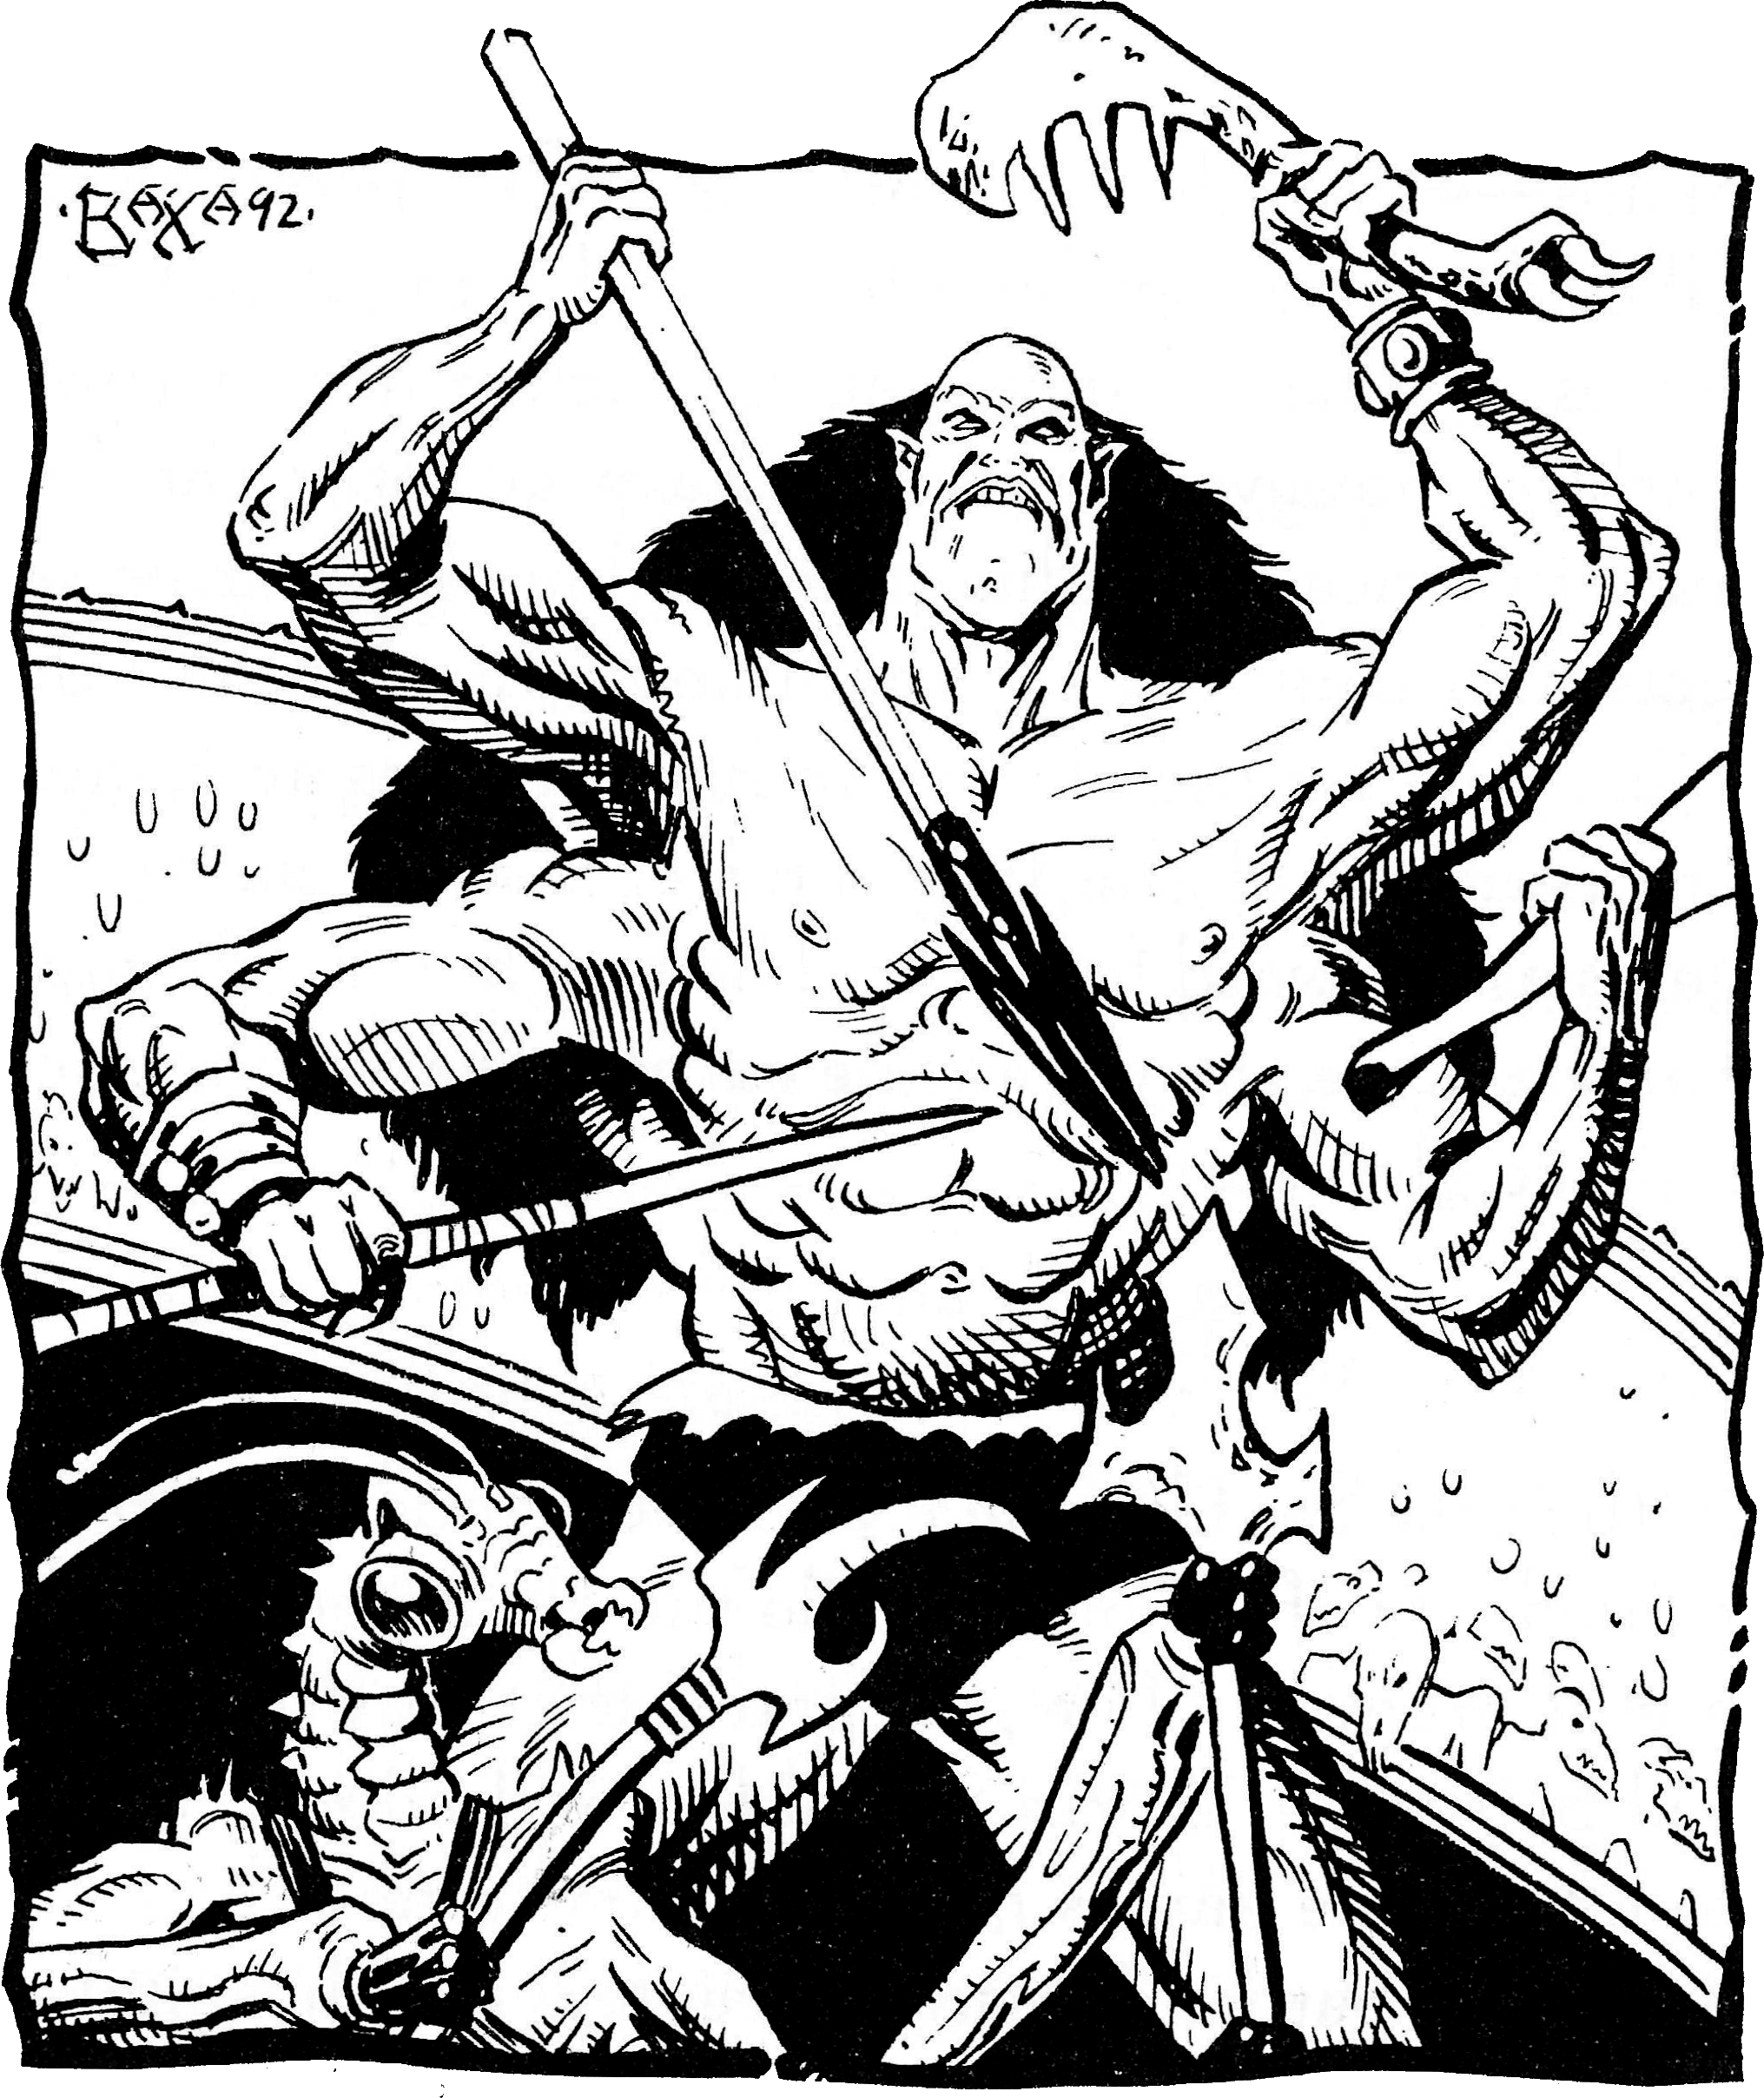
\includegraphics[width=\columnwidth]{images/b-rohg-2.png}
\WOTC
\end{figure}

B'rohgs have no mastery of fire but do not fear it. They also have no real understanding of death and will ignore objects or creatures that do not display signs of life (although they have learned that ``playing dead'' is a tactic sometimes used by their foes and will repeatedly strike felled enemies, just to be sure).

While they are too stupid to learn more contemporary speech, others can learn the grunt and sign language of the b'rohgs.

\subsubsection{B'rohg Racial Traits}
\begin{itemize*}
    \item +14 Strength, +4 Dexterity, +8 Constitution, $-4$ Intelligence: B'rohgs are stupid but very strong and agile.
    \item Huge: $-2$ penalty to Armor Class, $-2$ penalty on attack rolls, $-8$ penalty on \skill{Hide} checks, +8 bonus on grapple checks, lifting and carrying limits quadruple those of Medium characters.
    \item B'rohgs occupy a space of 4.5 meters and have a reach of 4.5 meters.
    \item Giant: B'rohgs are creatures with the giant type.
    \item B'rohg base land speed is 12 meters. B'rohg base climb speed is 6 meters. B'rohg have +8 racial bonus on \skill{Climb} checks. They can always choose to take 10 on a \skill{Climb} check, even if rushed or threatened.
    \item Low-light vision: B'rohgs can see twice as far as a human in moonlight and similar conditions of poor illumination, retaining the ability to distinguish color and detail.
    \item Racial Hit Dice: A b'rohg begins with 6 levels of giant, which provide 6d8 Hit Dice, a base attack bonus of +4, and base saving throw bonuses of Fort +5, Ref +2 and  Will +2.
    \item Racial Skills: A b'rohg's giant levels give it skill points equal to 9 $\times$ (2 + Int modifier). Its class skills are \skill{Climb}, \skill{Listen}, \skill{Spot} and \skill{Survival}.
    \item Racial Feats: A b'rohg's giant levels give it 3 feats.
    \item Weapon Proficiency: A b'rohg is proficient with simple and martial weapons as well as its natural weaponry.
    \item Natural Armor: +6 natural armor bonus to AC.
    \item Natural Weapons: 4 slams (1d6).
    \item Rock Catching (Ex): Once per round, a b'rohg that would normally be hit by a rock can make a Reflex save to catch a rock (or similar projectile) as a free action. The DC is 15 for a Small rock, 20 for a Medium one, and 25 for a Large one (if the projectile provides a magical bonus on attack rolls, the DC increases by that amount.) The b'rohg must be ready for and aware of the attack in order to make a rock catching attempt.
    \item Rock Throwing (Ex): Adult b'rohgs are accomplished rock throwers and receive a +1 racial bonus on attack rolls when throwing rocks. A b'rohg of at least Huge size can hurl rocks weighing 30 to 40 kilograms each (Medium objects) up to five range increments. The size of the range increment is 42 meters.
    \item Automatic Languages: B'rohg. Bonus Languages: none.
    \item Favored Class: Ranger.
    \item Level Adjustment: +9.
\end{itemize*}

\subsectionA{Belgoi}
Belgoi are a race of savage humanoids that appear human, but their blue skin, clawed hands and webbed, three-toed feet soon give it away. They have no teeth, no visible ears, and their hair is black and stringy.

Belgoi live in the most desolate of places, since no other race will allow them nearby. Belgoi seem to revel in destruction, and are considered to be second only to the defilers in the damage they do to the world around them.

\subsubsection{Belgoi Society}
Belgoi form large nomadic tribes that move into an area, strip it of all resources, and then move on. These tribes send out raiding parties that attack caravans and small villages, hoping to obtain food and treasure. They will eat anything but prefer the taste of the flesh of intelligent races.

These humanoids engage in trade from time to time. Their infamy makes them thoroughly objectionable, and their wares are full of the most distasteful items. However, anyone who still finds themselves trading with the belgoi discovers that they are reasonably honest in all dealings.

Belgoi speak their own language and the Common tongue.

\Figure{b}{images/belgoi.png}

\subsubsection{Belgoi Racial Traits}
\begin{itemize*}
	\item +4 Dexterity, $-4$ Intelligence, +4 Charisma: Belgoi are fast, but they are not smart.
    \item Humanoid (belgoi, psionic): Belgoi are humanoid creatures with the belgoi and psionic subtypes.
	\item Medium: Belgoi receive no advantages or penalties due to size.
    \item Belgoi base land speed is 9 meters.

    \item Darkvision: Belgoi can see in the dark up to 18 meters. Darkvision is black and white only, but it is otherwise like normal sight, and belgoi can function just fine with no light at all.

    \item Racial Hit Dice: A belgoi begins with five levels of humanoid, which provide 5d8 Hit Dice, a base attack bonus of +3, and base saving throw bonuses of Fort +1, Ref +1, and Will +4.
    \item Racial Skills: A belgoi's humanoid levels give it skill points equal to 8 $\times$ (2 + Int modifier). Its class skills are \skill{Hide}, \skill{Intimidate}, \skill{Listen}, \skill{Move Silently}, \skill{Search}, and \skill{Spot}.
    \item Racial Feats: A belgoi's humanoid levels give it 2 feats.
    \item Weapon Proficiency: A belgoi is proficient with all simple weapons and their natural weaponry.

    \item Natural Weapons: 2 claws (1d4).

    \item Constitution Damage (Ex): A belgoi's claw attack deals additional 1d6 points of Constitution damage.
    \item Naturally Psionic: Belgoi gain 35 bonus power points at 1st level. These power points can be used for their psi-like abilities or to manifest powers, if they gain levels in a psionic class.% is benefit does not grant them the ability to manifest powers unless they gain that ability through another source, such as levels in a psionic class.
    \item Bell Ringing (Ps): Belgoi can use a tiny bell to make \psionic{contact} wit a creature up to 600 meters away. Belgoi can't use this ability without a bell. The ability is otherwise identical to \psionic{contact} manifested by a 2nd-level manifester. The power check is Charisma-based.
    % \item Bell Ringing (Su): Belgoi use a bell to focus their \psionic{psionic dominate}. A \psionic{psionic dominate} target who hears the belgoi's bell receives a $-2$ penalty on their Will save.
    \item Psi-like Abilities:
        \psionic{attraction},
        \psionic{ego whip},
        \psionic{psionic blast},
        \psionic{psionic dominate}.
    Manifester level 2nd. The power checks and save DCs are Charisma-based.

    \item Automatic Languages: Belgoi. Bonus Languages: Common.
    \item Favored Class: Psion.
    \item Level Adjustment: +3.
\end{itemize*}

\subsectionA{Gith}
Gith are a lanky race of reptilian humanoids that, when erect, stand close to 2 meters tall, but who spend most of their time, bent-over in a crouch that makes them appear to be only 1.5 meter tall. Their lower jaws jut forward and, while toothless, they have sharp, bony ridges that they use to crush and grind their food. Their powerful legs allow them to make great leaps, which they use to move about, walking in an awkward waddle only when they cannot jump or when sneaking up on prey.

\subsubsection{Gith Society}
Gith organize themselves into tribes, with the most powerful member acting as leader. All authority comes from the chief, who has the power of life and death over any member of his tribe. If the chief is killed, the strongest members of the tribe will fight to the death in order to determine who will be the new leader. This trial-by-combat occurs immediately, even if the gith tribe is currently in the middle of a battle with another force.

Most gith tribes inhabit mountainous regions, coming down only to raid the villages of other humanoids or to attack a passing caravan. They are usually interested in entertaining themselves with the suffering of others and with the prospect of a good meal (gith will eat anything organic, preferring meat), but know the value of treasure, especially of psionic and magical items.

Gith speak their own language, which has no alphabet but can be expressed in elvish script.

\Figure{t}{images/gith.png}

\subsubsection{Gith Racial Traits}
\begin{itemize*}
    \item +2 Dexterity, $-2$ Intelligence, $-2$ Charisma: Gith have keen reflexes but are slightly dim and aggressive in their behavior.
    \item Humanoid (gith): Gith are humanoid creatures with the gith subtype.
    \item Medium: As Medium creatures, gith have no special bonuses or penalties due to size.
    \item Gith base land speed is 9 meters.
    \item Low-light vision: Gith can see twice as far as a human in moonlight and similar conditions of poor illumination, retaining the ability to distinguish color and detail.
    \item Natural Armor: Gith have a +2 natural armor bonus to AC due to their tough hide and heavy bones.
    \item Natural Weapons: 2 claws (1d4).
    \item Gith are natural jumpers, gaining a +10 racial bonus to all \skill{Jump} checks.
    \item Leaping Charge (Ex): Gith can use their leap to improve a charge. Whenever a gith charges and they jump at least 3 meters, they gain an additional +2 bonus on their attack roll. This bonus stacks with the +2 bonus given by charging.
    \item Gith have a +4 racial bonus on all \skill{Hide} and \skill{Move Silently} checks. Gith are sly and stealthy.
    \item Automatic Languages: Gith. Bonus Languages: Common, Elven, Pterran, Ssurran and Tarek.
    \item Favored Class: Rogue.
    \item Level Adjustment: +1.
\end{itemize*}

\Figure*[\textwidth-1cm]{t}{images/hej-kin.png}

\subsectionA{Hej-Kin}
Hej-kin are a race of degenerate humanoids that spend their entire lives underground, dwelling in the Athasian underdark near suitable supplies of water. They are omnivores and subsist largely on a diet of small subterranean creatures and plants.

Hej-kin are malevolent creatures that enjoy inflicting pain and fear on those who trespass on their caverns, blaming them for the damage that has been inflicted on the earth by the defilers.

Hej-kin language is a combination of sign and verbal communication, and their voices are low-pitched, resembling human mumbling. Few surface dwellers are able to learn the language. The color of their skin varies from red to light green, but their skin is always thick and very tough. Hej-kin live on average for 40 or 45 years.

\subsubsection{Hej-Kin Society}
Hej-kin do not create artificial tunnels or caves, as they consider the earth to be sacred. They will only occupy naturally-occurring subterranean formations, but they mark these as their property with curious runes on the cave walls.

Hej-kin clans are often led by earth clerics and preservers. Clerics rise highest in hej-kin society and are the only hej-kin who travel to the surface, usually investigating a disturbance that threatens the earth. Hej-kin are never defilers.

Hej-kin are natural enemies to most other surface dwelling and subterranean races, due to the abuse and destruction of the earth perpetrated by these others. Hej-kin clans will migrate to a new area every decade in order to avoid over-using the land on which they dwell.

\subsubsection{Hej-Kin Racial Traits}
\begin{itemize*}
    \item $-4$ Dexterity, +4 Wisdom, $-2$ Charisma: Hej-kin are not agile, and they don't understand the surface dwellers society.
    \item Humanoid (hej-kin, psionic): Hej-kin are humanoid creatures with the hej-kin and psionic subtypes.
    \item Small: Hej-kin gain a +1 size bonus to Armor Class, a +1 size bonus on attack rolls, and a +4 size bonus on \skill{Hide} checks, but they must use smaller weapons than humans use, and their lifting and carrying limits are three-quarters of those of a Medium character.
    \item A hej-kin's base land speed is 6 meters. They may phase through rock and earth at a speed of 3 meters.

    \item Darkvision: Hej-kin can see in the dark up to 18 meters. Darkvision is black and white only, but it is otherwise like normal sight, and hej-kin can function just fine with no light at all.

    \item Racial Hit Dice: A hej-kin begins with 2 levels of humanoid, which provide 2d8 Hit Dice, a base attack bonus of +1, and base saving throw bonuses of Fort +3, Ref +0, and Will +0.
    \item Racial Skills: A hej-kin's humanoid levels give it skill points equal to 5 $\times$ (2 + Int modifier). Its class skills are \skill{Hide}, \skill{Listen}, \skill{Spot} and \skill{Survival}.
    \item A hej-kin's humanoid levels give it one feat.
    \item Weapon Proficiency: A hej-kin is proficient with its natural weapons and all simple weapons.

    \item Natural Armor: +1 natural armor bonus to AC.
    \item Natural Weapons: 2 claws (1d4).

	\item Hej-kin receive a +30 circumstance bonus on \skill{Hide} checks while phased inside solid rock.
    \item Phase (Su): Hej-kin may move through earth and rock at a speed of 3 meters. They may stop while inside of walls or floors and remain there indefinitely.
	\item Poison (Ex): A hej-kin delivers its poison with a successful claw attack. Fortitude DC 11 + Con modifier. The initial and secondary damage are 1 Con.
    \item Resistant Mind (Su): Hej-kin have naturally developed psionic defenses. Any psionic attack against a hej-kin has a $-3$ penalty. This effect is always active while the hej-kin has available power points.

    \item Psionic Powers: A hej-kin character manifests psionic powers as a 2nd-level psion. If the character takes additional levels of psion, these levels stack with the hej-kin's base manifesting ability for powers known, power points per day, and other effects dependent on manifester level. A hej-kin character likewise uses the sum of its racial spellcasting levels and class levels to determine the abilities of its psicrystal.

    \item Automatic Languages: Hej-kin. Bonus Languages: Anakore, Common, Elven, and Gith.
    \item Favored Class: Cleric.
    \item Level Adjustment: +2.
\end{itemize*}

\Figure*{t}{images/jozhal.png}

\subsectionA{Jozhal}
Jozhals are small, lightly built reptilian creatures which may be distantly related to crodlu. They have long, slender legs, lanky arms ending in dexterous hands, and long, flexible tails. The neck of a jozhal is also long and flexible, ending in a narrow-muzzled head with large eyes and many needle-like teeth. The skin is covered in many tiny scales, which are only visible on close examination, and can change color to match with or contrast against the creature's surroundings. Jozhals have precise control over their skin's color, and sometimes use it to create decorative patterns of color resembling tattoos.

\subsubsection{Jozhal Society}
Jozhals are naturally shy and secretive creatures, and do not normally learn the languages of other races. The leader of a family will learn the Common tongue, so that he or she may communicate with outsiders on the rare occasion that interaction is necessary. When around those they do not know, especially other races, jozhals become much more withdrawn and are unwilling to even speak to outsiders unless necessary. They will often travel days out of their way just to avoid encountering non-jozhals, especially elves and humans, whom they consider destructive. If forced to interact with members of another race, jozhals will attempt to make the experience as short as possible. Jozhals do not normally form permanent settlements. Instead, they travel in nomadic family groups, traveling between the fertile areas of the Tablelands and Hinterlands, beyond the Ringing Mountains. These families forage for roots, nuts, and small reptiles and insects. Jozhals always make use of every little bit of anything that they find, to the point of extremes, practicing cannibalism and fashioning the bones of their dead into weapons and tools. The only time a jozhal family will permanently settle in one area is when a member of that family becomes a grove master and takes custody of his guardian lands.

Jozhals are deeply suspicious of all arcane spellcasters. They will tolerate preservers, but will watch them closely for any signs that they may defile, and criticize them harshly if they use magic wantonly or carelessly. Jozhals do not tolerate defilers in any way. A jozhal may even put himself at risk to stop a defiler from damaging the land. The jozhal suspicion of arcane magic does not extend to magical items. Jozhals are fascinated by magical items, which they consider to hold the power of the land, and desire to own as may magical items as they can. Jozhal children are taught from a young age the proper use of magical items, both arcane and divine, so even non-spellcaster jozhals will be able to use most any magical item they come to possess. They go to great lengths to possess magical items, typically following parties of humanoids to determine if they carry any magical items and stealing any they detect.

Jozhal is a language composed of click, pops, and whistles. Do to its unusual nature, many who are not familiar with Jozhal will not even recognize it as a language. The vast majority of jozhals do not keep a written form of their language, and the pyreen alphabet is the only known writing system that can be adapted to writing the jozhal tongue.

\subsubsection{Jozhal Racial Traits}
\begin{itemize*}
    \item $-4$ Strength, +4 Dexterity, $-2$ Constitution, +4 Intelligence, +4 Wisdom.
    \item Aberration: jozhals are not subject to spells or effects that affect humanoids only, such as \spell{charm person} or \spell{dominate person}.
    \item Small: jozhals gain a +1 size bonus to Armor Class, a	+1 size bonus on attack rolls, and a +4 size bonus on \skill{Hide} checks, but they must use smaller weapons than humans use, and their lifting and carrying limits are three-quarters of those of a Medium character.
    \item A jozhal's base land speed is 15 meters.

    \item Racial Hit Dice: A jozhal begins with four levels of aberration, which provide 4d8 Hit Dice, a base attack bonus of +3, and base saving throw bonuses of Fort +1, Ref +1 and Will +4.
    \item Racial Skills: A jozhal's aberration levels give it skill points equal to 7 $\times$ (2 + Int modifier). Its class skills are \skill{Climb}, \skill{Concentration}, \skill{Hide}, \skill{Jump}, \skill{Knowledge} (arcana), \skill{Listen}, and \skill{Use Magic Device}.
    \item A jozhal's aberration levels give it 2 feats.
    \item Weapon Proficiency: A jozhal is proficient with all simple weapons and its natural weaponry.

    \item +4 racial bonus on \skill{Hide} checks. Jozhals can alter their skin coloration and often use this for camouflage purposes.
    \item +4 racial bonus on \skill{Use Magic Device} checks. Jozhals have a natural affinity for magic.

    \item Natural Armor: +4 natural armor bonus to AC.
    \item Natural Weapons: Bite (1d8).

    \item Psionic Powers: A jozhal character manifests psionic powers as a 4th-level psion. If the character takes additional levels of psion, these levels stack with the jozhal's base manifesting ability for powers known, power points per day, and other effects dependent on manifester level. A jozhal character likewise uses the sum of its racial spellcasting levels and class levels to determine the abilities of its psicrystal.
    \item Spells: A jozhal character casts spells as a 4th-level elemental cleric---jozhal are never paraelemental clerics. If the character takes additional levels of cleric, these levels stack with the jozhal's base spellcasting ability for spells per day, and other effects dependent on caster level. A jozhal character likewise uses the sum of its racial spellcasting levels and class levels to determine the abilities of their domain granted powers.
    \item Spell Resistance (Ex): A jozhal has spell resistance equal to 9 + class levels.

    \item Automatic Languages: Jozhal, Common. Bonus Languages: Aarakocra, Dwarven, Elven, Pterran, and Thri-Kreen.
    \item Favored Class: Cleric.
    \item Level Adjustment: +3.
\end{itemize*}

\subsectionA{Scrab}
Scrabs are small, insectoid men that live in nests in the desert. A scrab can draw air through sand while submerged due to the long gills located all along the grooves in their shells. Scrabs are ruled over by monstrously bloated members of the species known as nest mothers.

Scrabs need very little water to survive and seem to derive all the sustenance that they need from the blood and other bodily fluids of their victims.

Scrabs can speak their own language. A small percentage can also speak elvish. Adult scrabs live to be 25 years old, but nest mothers can live twice that long.

\Figure{t}{images/scrab.png}

\subsubsection{Scrab Society}
Scrabs inhabit tunnels deep under the desert, which they fashion using spittle that solidifies the sand. If possible, the entrance to the nest will be concealed behind a rocky outcrop. Scrabs hate elves and prefer their flesh above that of any other creature. This hatred extends beyond a desire for food and, in fact, anything with pointed ears is likely to be identified as an elf. A captive elf may be kept alive for weeks, even months, just to be tortured. Legends of both races hold that there were once great wars between the two species, with each side blaming the other for the conflicts and for the many unspeakable atrocities perpetrated on innocent victims of each race.

The eldest male in the nest is allowed to mate with the nest mother, with clutches of up 100 eggs resulting. The eggs hatch in three months, and the young are possessed by a cannibalistic frenzy when they are born. Fewer than half the hatchlings survive this period. Three quarters of all hatchlings are male.

Only males who develop additional psionic abilities or spellcasting powers grow into leaders, and only females with clerical abilities can become nest mothers. A female who begins to develop into a nest mother will take a number of males and depart to create a new nest of her own.

Scrabs are predators first and foremost but will trade with merchants brave enough to risk contact with the creatures. They are also preyed upon by the larger creatures that inhabit the wastes. Part of the scrabs' hatred of elves stems from the fact that elves use every part of a scrab they have defeated. A scrab shell can be used to make breastplates, and the sharp parts of the pincers make decent polearms.

\subsubsection{Scrab Racial Traits}
\begin{itemize*}
    \item +4 Intelligence, +2 Wisdom.
    \item Monstrous Humanoid: Scrabs are not subject to spells or effects that affect humanoids only, such as \spell{charm person} or \spell{dominate person}.
    \item Small. Scrabs gain a +1 size bonus to Armor Class, a +1 size bonus on attack rolls, and a +4 size bonus on \skill{Hide} checks, but they must use smaller weapons than humans use, and their lifting and carrying limits are three-quarters of those of a Medium character.
    \item A scrab's base land speed is 15 meters. Scrabs also have a burrow speed of 3 meters.
    \item Darkvision: Scrabs can see in the dark up to 18 meters. Darkvision is black and white only, but it is otherwise like normal sight, and scrabs can function just fine with no light at all.
    \item Racial Hit Dice: A scrab begins with 5 levels of monstrous humanoid, which provide 5d8 Hit Dice, a base attack bonus of +5, and base saving throw bonuses of Fort +1, Ref +4 and Will +4.
    \item Racial Skills: A scrab's monstrous humanoid levels give it skill points equal to 8 $\times$ (2 + Int modifier). Its class skills are \skill{Concentration}, \skill{Hide}, \skill{Listen}, \skill{Move Silently}, \skill{Psicraft}, \skill{Spot}, and \skill{Survival}.
    \item A scrab's monstrous humanoid levels give it 2 feats.
    \item Weapon Proficiency: A scrab is proficient with its natural weaponry and all simple weapons.
    \item Natural Armor: +5 natural armor bonus to AC.
    \item Natural Weapons: 2 claws (1d4).
    \item Improved Grab: To use this ability, a scrab must hit with a claw attack. It can then attempt to start a grapple as a free action without provoking an attack of opportunity. If it wins the grapple check, it deals automatic claw damage each round it remains grappling.
	\item Psionic Powers: A scrab character manifests psionic powers as a 5th-level psion. If the character takes additional levels of psion, these levels stack with the scrab's base manifesting ability for powers known, power points per day, and other effects dependent on manifester level. A scrab character likewise uses the sum of its racial spellcasting levels and class levels to determine the abilities of its psicrystal.
    \item Automatic Languages: Scrab. Bonus Languages: Common, Elven, Entombic.
    \item Favored Class: Psion.
    \item Level Adjustment: +3.
\end{itemize*}

\subsectionA{Silt Runner}
Silt runners are a race of short lizard-men with green scales, jagged teeth, and wickedly clawed hands. They are cowardly reptilian humanoids with the curious ability to run across open silt. They have tails, but these usually drag along the ground except when they are running or in combat, when the tail is used to help them maintain their balance. They wear trophies taken from their victims.

\subsubsection{Silt Runner Society}
Most silt runner tribes live on islands of the Silt Sea near the coastline, the same islands that giants live. Giants view them as pests overrunning their homes, and are left alone by silt runners, since they are just too fast to swat properly.

Silt runners live by raiding passing merchant caravans and nearby villages. Silt runners have an unreasoning hatred for elves and attack them on sight---they may even turn aside from a caravan to attack a single elf. They consider the flesh of an elf slain in combat to be the greatest of delicacies.

Silt runners speak a tribal language, and a few of them can
speak Common.

\Figure{t}{images/silt-runner.png}

\subsubsection{Silt Runner Racial Traits}
\begin{itemize*}
    \item $-4$ Intelligence, $-2$ Charisma.
    \item Humanoid (psionic, reptilian): Silt runners are humanoid creatures with the psionic and reptilian subtypes.
    \item Small. Silt runners gain a +1 size bonus to Armor Class, a +1 size bonus on attack rolls, and a +4 size bonus on \skill{Hide} checks, but they must use smaller weapons than humans use, and their lifting and carrying limits are three-quarters of those of a Medium character.
    \item A silt runner's base land speed is 42 meters.
    \item Darkvision: Silt runners can see in the dark up to 18 meters. Darkvision is black and white only, but it is otherwise like normal sight, and silt runners can function just fine with no light at all.
    \item Weapon Proficiency: A silt runner is proficient with all simple weapons and its natural weaponry.
    \item +4 racial bonus on \skill{Balance} checks. A silt runner's tail makes them exceptionally stable.
    \item Natural Armor: +2 natural armor bonus to AC.
    \item Natural Weapons: A silt runner's primary attacks are two claws (1d3), and their secondary attack is their bite (1d6).
    \item Silt Run (Ex): A silt runner moving at running speed can move across up to 18 meters of silt without breaking the surface.
    \item Psi-Like Abilities: 1/day---\psionic{anchored navigation}, \psionic{precognition}, \psionic{synesthete}. Manifester level equal to the silt runner's class levels.
    \item Automatic Languages: Silt Runner. Bonus Languages: Common.
    \item Favored Class: Rogue.
    \item Level Adjustment: +1.
\end{itemize*}

\Chapter{Organizations}
{Traders cooperate for Profit. Templars form allegiances for Domination. Psions join schools to gain Knowledge. And raiders band together for Strength. Power comes in many forms, but all who band together seek it---intentionally or unknowingly. Those who join them are caught in a web, for all organizations are tainted with corruption. The Veiled Alliance seeks to overthrow the Sorcerer-Kings and justifies murder in its ranks out of fear for discovery. The elitist Order would deny all other beings the use of psionic power and drive tens of thousands of beings insane. And the first generation dray believe they are children of a god, who has banished them from their homes. Once you realize the secrets of your organization, it is too late, for you are shackled to it. You realize you have traded your freedom for power.}{The Oracle, Blue Shrine Scrolls}

In a {\tableheader Dark Sun} campaign, characters may have to deal with intrigue and sabotage as often as with creatures of the Athasian wastelands. The descriptions that follow represent only a few of the many organizations that operate across the Tablelands and beyond. Some can be used as patrons for adventurers, other as opponents. More often, these organizations can be an ally one day, and opponent the next.

\section{Dynastic Merchant Houses}

\textbf{Entry Requirements:} Accept the Merchants' Code (see below).

It would be a terrible mistake to assume that all power on Athas rests in the hands of the sorcerer-kings. Power can be held in many ways, and many hands besides those of the cities' rulers may possess it.

The merchant houses supply the lifeblood of Athas---foodstuffs that feed isolated city‐states, construction materials to build the palaces of sorcerer-kings and decadent nobles, slaves to toil in fields or fight and die in gladiator pits, and many other vital items.

\subsubsection{Merchants' Code}
All mercantile houses follow a strict code of behavior, known as the Merchants' Code. Anyone wishing to join a merchant house must accept all aspects of this code and abide by them or face immediate expulsion. The code varies from house to house, but in most cases it conforms to the following principles:

\begin{enumerate*}
\item Recognition that by joining a merchant house, an agent forsakes citizenship in any city or membership in any tribe.
\item An oath of allegiance to the merchant house.
\item A promise to perform in the best interests of the merchant house in return for a salary.
\item A promise to deal honestly with stranger, friend, and foe alike.
\item A promise not to flaunt any wealth gained through employment with the house.
\item A promise to uphold the laws of the city in which the agent is stationed, and to do nothing to bring down the wrath of the sorcerer-king or his agents upon the house.
\item A promise to cooperate with other merchants to make life very expensive for any person who unjustly imprisons, blackmails, or otherwise harasses any merchant.
\end{enumerate*}

\subsubsection{Dynastic Merchant Houses Benefits}
Being a member of any merchant house gives access to some common benefits.

\textbf{Economics:} Agents of a Merchant House may buy their House's specialty goods for 80\% of their listed market price.

\textbf{Services:} Merchant Houses often acquire hirelings for their caravans. Agents may get access to experts among the hirelings to appraise, disguise, and negotiate. These experts have a relevant skill modifier of +10. Experts with modifiers of +15 or higher are also available at half the price.

\textbf{Information:} Checking with the leader of the local headquarters is equivalent to a \skill{Gather Information} check on the PCs' behalf. A typical House local leader has a \skill{Gather Information} modifier of +15.

\textbf{Access:} Agents have access to a place to stay in each city-state, and in each of the House's facilities.

\subsubsection{Dynastic Merchant Houses in the Game}
Senior members of a Merchant House make good patrons and allies. They might seek to hire the PCs for almost any kind of mission or even recruit them if they display useful skills. As a twist, you can use a templar to send the PCs on various missions, revealing only later (or not at all) that the PCs' contact is actually an undercover agent from a Merchant House. Allow the PCs to take advantage of the hirelings, special transportations, and other perks of joining a Merchant House. Over time, introduce the costs associated with those advantages: internal and interhouse rivalries, political machinations, and the feeling of being just a small cog in a vast economic enterprise.

\subsection{House Inika}
\textbf{Location:} Gulg.

\textbf{Banner:} A plain gold circle on a black field.

\textbf{Trade Goods:} Small and valuable items such as Kola nuts, spices, gems, feathers.

\textbf{Troops:} 500 soldiers (5th level or higher).

Inika operates out of its headquarters in the city of Gulg. It is small compared to some of the other major houses, but this is by choice. Dealing in small, valuable cargoes, such as kola nuts, exotic feathers, spices, and gemstones, Inika sees the benefit in remaining small and efficient. As a result, the house rakes in profits far out of proportion to its size, gaining a reputation for being one of the shrewdest houses in the region.

\subsubsection{Brief History}
Over three centuries ago, in the year of the Desert's Fury, in the city of Gulg, Taro Inika, a trusted agent of House Riben, broke his merchant's oath and left his employers, starting his own house. Only the good will of Biria Riben, the house's matriarch who had once been Inika's lover, prevented the new house from being crushed within a year.

In Gulg, rivalries between trade houses are kept to a minimum to maintain the peace and tranquility of the city. This proved a rich environment for the new concern. Within a few years, the house assumed its current form: a streamlined business dealing in small but valuable cargoes.

The House Inika's major philosophies are that force is to be used only as a last resort, and that strategic withdrawal to a superior position is often the best route.

\subsubsection{Inika's Assets}
Gulg's relative tranquility and the regularity of its production provides House Inika with a regular income. Wise investment and conservative spending combine to keep Inika on a solid financial footing.

\textbf{Caravans:} Inika's caravans are small and fast. Elven scouts provide advance warning of ambushes or attacks, which are usually avoided rather than confronted. Cargo is carried almost exclusively on kanks, although inix are sometimes used for larger cargoes. Mekillots and wagons are almost never found in Inika caravans.

Average caravans include about a dozen elven scouts with up to 20 kanks and (rarely) four to six inix. Due to the caravans' small size, House Inika can afford to maintain many more than other merchant houses. At any one time, Inika can have 50 to 75 caravans carrying cargo across the region.

Inika caravans' tactics are, first and foremost, to avoid any enemy forces. Should this fail, they scatter to break up pursuit. The scouts are expected to seek out the dispersed kank riders and bring them back together after the attack has ended.

\textbf{Facilities:} House Inika maintains very few permanent installations, preferring to temporarily rent or lease space in villages, forts, or cities.

\textit{Fort Adros:} 75 employees, 150 slaves. Supply point along the gold route between Walis and Altaruk. Often a target of attacks by elves and gith.

\textit{Fort Harbeth:} 50 employees, 100 slaves. A major trading post for the slaves of Salt View and a place to purchase dwarven items from Ledopolus.

\textit{Fort Skonz:} 50 employees, 75 slaves. Supply point at junction of three roads between Tyr, Altaruk, and Silver Spring.

\textit{Shazlim:} Trade village, 500 citizens. Located along the southern edge of Dragon's Bowl between Raam and Silver Spring, Shazlin represents an important stopover and trade point in the area.

\subsubsection{House Inika in Athas}
House Inika stays out of trouble. This is not to say that Inika never engages in intrigue or double-dealing; it's just very difficult to catch Inika at it. Such conduct is usually directed only at those who have done wrong by Inika. House Inika does not get mad, but it does get even.

In dealing with other houses and the sorcerer-kings, Inika takes a nonconfrontational approach. If challenged for control of an important route or commodity, Inika resists strongly to persuade its opponents to commit time and resources to the conflict. Inika then withdraws suddenly, changes tactics, and ends up putting pressure on the opponents in a totally unexpected quarter.

\subsubsection{Inika Lore}
Characters with ranks in \skill{Knowledge} (local [Gulg]) or \skill{Gather Information} can research House Inika to learn more about it. When a character makes a skill check, read or paraphrase the following, including the information from lower DCs.

\textbf{DC 10:} House Inika is the major merchant house in Gulg.

\textbf{DC 15:} Inika is dedicated in trading spices, gemstones and other luxury items.

\textbf{DC 20:} Caravans are small and fast, in order to minimize the losses from raids. Becoming an agent for Inika is safe and profitable, even being their slave is not (that) bad---just don't cross them in any way.

\textbf{DC 25:} Their tactic is to stay out of trouble from other houses.  If it comes to it, they hit where it hurts. 

\textbf{DC 30:} House Wavir in Balic is counted as an ally by House Inika. Most others at least have nothing against House Inika, though trade rivalries are common. House Tsalaxa harbors bad feelings toward Inika, but Inika's reputation prevents Tsalaxa from taking overt action.

A bardic knowledge check can reveal the same information as these knowledge checks, but in each case the DC is 5 higher than the given value.

\subsubsection{Agents}
Should a hireling rise through the ranks to become a valued employee, however, House Inika may offer the ultimate honor---a permanent position as an agent. Particularly successful agents may be invited to join the family itself, but this is very rare.

Agents are well cared for, due in part to their small numbers. Inika is reluctant to share its prosperity with too many house members, so its agents are few but highly skilled. Inika cares for its agents and their families from the cradle to the grave, on the wise thought that such a major investment is not lightly set aside.
\textbf{Wages:} Hirelings receive average pay, at most. Agents are well cared for all their needs.

\textbf{Additional Requirements:} Base attack bonus +6, \skill{Diplomacy} 13 ranks.

\textbf{Desired Roles:} Scouts, spies, kank riders, and lightly armed, fast-moving fighters. Mages and psionicists only in dire need.
\subsection{House M'ke}
\textbf{Location:} Raam.

\textbf{Banner:} A silver quill pen on a red field.

\textbf{Trade Goods:} Metals, food, weapons, and obsidian.

\textbf{Troops:} 600 soldiers.

As chief house of the troubled city of Raam, M'ke maintains a precarious balance between the reviled Great Vizier and the restive populace. The house's reputation has fallen somewhat in recent years due to the near-anarchy in Raam, but M'ke has fallen back on its vast cash reserves to see it through.

\subsubsection{Brief History}
House M'ke's origins are somewhat mysterious. Some claim that the house originated in an unknown area beyond the Tyr region, while others believe that M'ke was founded by dissident templars fleeing their sorcerer-king's wrath. Whatever its origin, M'ke became a force to be reckoned with.

M'ke's subsequent behavior has been an interesting combination of ruthlessness and caution. They treat more powerful rivals with intense respect, but they steal trade routes and even engage in open combat with weaker houses. Despite their occasional vicious streak, members of House M'ke are generally considered pleasant and intelligent individuals with few bad habits. This is only one of many bizarre contrasts in the confusing, contradictory House M'ke.

Trade by the house has shrunk of late, with M'ke withdrawing to secure citadels and outposts and adopting a fortress mentality to withstand the chaos in Raam. Truvo M'ke realizes that this means the future will hold intense struggles to regain old routes, but the house has been equal to the task in the past.

\subsubsection{M'ke's Assets}
M'ke's greatest asset is its hidden wealth, much of which is contained in the vaults beneath the family palace in Raam. Other caches of wealth are rumored to be scattered throughout the Tyr region as a hedge against future reverses.

\textbf{Caravans:} M'ke can maintain only ten to 20 caravans at any one time. A typical caravan consists of 20-30 crodlu-mounted scouts, six to ten medium-sized wagons and, on especially important caravans, up to four well-defended armored caravan wagons. Crossbow-armed troops ride in the caravans, while foot soldiers or slaves walk alongside to provide further protection.

\textbf{Facilities:} House M'ke's holdings have shrunk along with their caravan routes. The house maintains small offices, often with skeleton staffs, in most major cities of the Tyr region.

\textit{Fort Firstwatch:} 30 employees, 50 slaves. Storage and supply point between Raam and Draj. Frequent target of raids by trade rivals and elf nomads.

\textit{Fort Isus:} 50 employees, 100 slaves. Supply point and trading post between Raam and Nibenay. Popular spot for trading with nomadic tribes.

\textit{Fort Xalis:} 100 employees, 150 slaves. Major trading post, supply point, and military base near Black Waters, between Raam and Urik. Much of M'ke's reduced military manpower has been concentrated here, because the obsidian and slave routes between Raam and Urik are vital to Raam's survival and M'ke's continued prosperity.

\textit{Jalaka:} Trade village, 250 citizens. Despite difficult terrain and massive logistical problems, M'ke continues to maintain this village, located on the edge of the Forest Ridge approximately 60 kilometers north of Tyr.

\subsubsection{House M'ke in Athas}
Powerful rivals are treated with respect and even friendship, while weaker houses are treated with contempt. M'ke's mercenaries have few qualms about raiding the caravans of small houses or even assaulting their headquarters or warehouses in major cities. Perhaps the best way for a small house to deal with M'ke is to put up a bold front, for M'ke will pounce at the slightest sign of weakness.

M'ke also treats the sorcerer-kings with great respect, even going so far as to maintain strict neutrality while the rest of Raam's populace calls for the Great Vizier's overthrow. M'ke never engages in smuggling, and it is particularly friendly with the kings of Draj and Urik.

\subsubsection{M'ke Lore}
Characters with ranks in \skill{Knowledge} (local [Raam]) or \skill{Gather Information} can research the House of the Mind to learn more about it. When a character makes a skill check, read or paraphrase the following, including the information from lower DCs.

\textbf{DC 10:} House M'ke is the major merchant house in Raam.

\textbf{DC 15:} M'ke trades in food and weapon supplies.

\textbf{DC 20:} They can't maintain many caravans at the same time, 20 at most. Becoming an agent for M'ke is busy work---and dangerous. They pay much better than most, but it is dangerous to switch houses.

\textbf{DC 25:} M'ke is shrinking lately, but they still maintains a halfling village. The reasons for this persistence are the profits to be gained from the hardwood found in the forest and the unique trade goods from the halflings of the forest. Some also suggest that Jalaka harbors a major cache of M'ke's wealth, though no specifics of this alleged hoard are known.

\textbf{DC 30:} Houses Vordon and Tsalaxa have been applying pressure on M’ke of late, urging it to join the rebels seeking to overthrow the Great Vizier, but so far nothing has come of this.

A bardic knowledge check can reveal the same information as these knowledge checks, but in each case the DC is 5 higher than the given value.

\subsubsection{Agents}
Unfortunately, the mortality rate among M'ke employees, who are expected to die rather than betray or compromise their masters, is quite high. Employees who transfer loyalty (when offered higher wages, for example) are dealt with harshly. Hirelings must obtain permission from the top in order to change employers.

Work with M'ke is high-paying but hazardous, and new employees can expect constant action, including dealing with raids from outside tribes, nobles, and even rival merchant houses.

\textbf{Wages:} 25--50\% more higher wages than average. Special bonuses are paid for particularly resourceful or skilled acts in battle.

\textbf{Additional Requirements:} \skill{Bluff} 5 ranks, \skill{Diplomacy} 5 ranks; or ability to manifest 1st-level psionic powers.

\textbf{Desired Roles:} Bards, rogues, and psionicists are often employed; raamite templars have been known to offer services as guards, spies, or spellcasters.
\subsectionA{House Shom}
\textbf{Location:} Nibenay.

\textbf{Banner:} Three white dragonflies on a red-and-black, diagonally divided field.

\textbf{Trade Goods:} Obsidian, rice, water, wood, as well as a host of minor products, such as weapons and works of art.

\textbf{Troops:} 2,000+ soldiers.

House Shom, the leading trade faction in the city of Nibenay, is an old and (in the eyes of many) corrupt house. Perhaps the decadent atmosphere of Nibenay has affected the house's rulers, making them strange and merciless. Perhaps centuries of sybaritic luxuries have dulled their minds and convinced them that any means of making a profit is acceptable.

\subsubsection{Brief History}
Shom may be the oldest trading house in the Tyr region, with a history that stretches back for over a thousand years. The house's origins are shrouded in mystery and legend, but Nibenay's historians are certain that until eight centuries ago, Shom was a tiny house with a few secure trade routes and little ambition. It was when a young merchant named Kys came to power after the unexplained deaths of both his grandfather and mother that House Shom began to grow in size and influence. Nowadays, as the house's fortunes wane and its rulers grow more isolated, some claim that House Shom's masters have become sorcerer-kings themselves, in all but name.

Kys forged alliances with thri-kreen tribes, and to this day, belgoi are sometimes employed by House Shom---an unpleasant surprise for those who attack Shom's caravans. It is not known how Shom maintains friendly relations with these hostile creatures.


\subsubsection{Shom's Assets}
House Shom's assets are truly impressive. Unfortunately, much of the house's wealth is tied up in massive mansions and extravagant art treasures. The actual volume of trade the house engages in has shrunk steadily over the past few decades.

\textbf{Caravans:} Today, perhaps 20 caravans fly Shom's white dragonflies; these numbers decline each year. A typical Shom caravan employs 20 to 50 kank- or crodlu-mounted outriders, (who usually stick close to the main body of the caravan, thus defeating their purpose), as many as 150 leather-armored infantry, up to ten half-giants, and up to 20 mul gladiators who serve as guards for any family members or senior agents with the caravan. Family members rarely accompany caravans, but when they do, it is in a private mekillot wagon with extensive facilities.

\textbf{Facilities:} Typical outposts feature rather spartan quarters for the mercenary guards and outrageously extravagant quarters for the family member or agent assigned to command.

\textit{Fort Melidor:} 60 employees, 150 slaves. Supply point located near Lost Oasis. Most of the time, the fort sits idle, waiting for family members to visit.

\textit{Fort Inix:} 75 employees, 200 slaves. Supply and storage point located at oasis 45 kilometers east of Nibenay. It is sometimes raided by slaves from Salt View or by various desert tribes, but in general it is a dull place.

\textit{Fort Sunset:} 25 employees. A tiny outpost in the shelter of the Ringing Mountains. It is quite impoverished, but it occasionally services a Shom caravan or fights off an attack by gith.

\textit{Cromlin:} Trade village, 300 citizens. Located on the shore of the Sea of Silt, 45 kilometers west of Giustenal. Cromlin serves as a trading city for nomadic tribes. It also maintains facilities for the repair and storage of silt skimmers, which many trading houses use to cut across the sea and reduce travel time between Nibenay and Raam.


\subsubsection{House Shom in Athas}
House Shom generally does not deign to acknowledge that any other merchant houses even exist; their attitude toward the mighty sorcerer-kings is only slightly better. Aggressive houses, particularly the militaristic House Stel, have engaged in an active campaign of raiding and disruption of Shom's routes between Nibenay and Raam.

Despite its diminished status, Shom maintains good relations with several tribes of thri-kreen, as well as numerous belgoi raiders. Those who attack Shom caravans or outposts occasionally find themselves confronted by unexpected hordes of mantis warriors or belgoi in disguise. 

Outsiders dealing with Shom usually have an easy time if they have enough cash for bribes. Shom agents can be persuaded to almost any course with enough ceramic pieces, although reform-minded agents respond to attempted bribes with disdain or even violence.

\subsubsection{Shom Lore}
Characters with ranks in \skill{Knowledge} (local [Nibenay]) or \skill{Gather Information} can research House Shom to learn more about it. When a character makes a skill check, read or paraphrase the following, including the information from lower DCs.

\textbf{DC 10:} House Shom is the major merchant house in Nibenay.

\textbf{DC 15:} Shom trades mainly in food supplies from the Crescent Forest, but also weapons and art. A typical Shom caravan is large and slow-moving, burdened by far more troops than it really needs, and numerous employees who do little more than take up cargo space.

\textbf{DC 20:} Shom has been shrinking over the past few decades, now they can maintain up to 20 caravans at the same time. Family members are always in the padded, silken confines of their vast mansions and isolated villas.

\textbf{DC 25:} House Shom has good relations with many thri-kreen tribes, even belgoi. But these relations are becoming brittle as the family is directing all their wealth to defend their house against enemies.

\textbf{DC 30:} A few of Shom's younger members have realized the dire straits their house is in, and they have begun to move to counteract this peril.

A bardic knowledge check can reveal the same information as these knowledge checks, but in each case the DC is 5 higher than the given value.

\subsubsection{Agents}
More than any other house, Shom depends on agents and hirelings for its survival. Since the members of the Shom family are loathe to even acknowledge the need for profit and mercantile practices, what remains of House Shom's once-vast influence is in the hands of the few agents who retain a shred of loyalty.

For their part, agents only rarely allow hirelings to rise through the ranks to the position of agent. For this reason, there is a great deal of intrigue and double-dealing among the employees of House Shom.

\textbf{Wages:} Up to double normal rates.

\textbf{Additional Requirements:} Base Fortitude save +3; must not have a power point reserve.

\textbf{Desired Roles:} Fighters, rangers, and gladiators are the most commonly employed. Clerics are also among the most desired roles. Shom's agents are paranoid with manifesters, distrusting anyone who might be able to discern their secrets. Shom has few qualms about hiring defilers, but they are hired only on a short-term basis.
\subsectionA{House Stel}
\textbf{Location:} Urik.

\textbf{Banner:} A pair of crossed black scimitars on a white field.

\textbf{Trade Goods:} Slaves, iron, gold, weapons, plundered items.

\textbf{Troops:} 3,000+ soldiers (3rd level or higher).

Closely associated with the warrior culture of Urik, Stel is without question the most aggressive and militaristic of the merchant houses. While Stel also maintains regular trade routes (albeit heavily guarded ones) and engages in ordinary trade, the house is best known for their specialization in the spoils of war.

\subsubsection{Brief History}
No one who lives in Urik for any amount of time remains unaffected by the city's omnipresent militarism; House Stel is no exception. Founded by a small group of warriors and gladiators nearly 300 years ago, and led by a soldier of fortune named Korvo Stel, the house would not have lasted long without the assistance and good will of the sorcerer-king.

Korvo built up an impressive trade house whose bases, outposts, and caravans were organized along strict military lines. But what the House Stel had in military strength, they lacked in business insight---they had little talent for selecting profitable cargoes or for managing the money the caravans brought in.

After several years of hiring outsiders to help the House's financial disaster, Iol, leader of Korvo's advisors and a talented psionicist, came to Korvo with an ultimatum. He wanted to be made a full partner in House Stel, and his fellows to be made part owners as well. Korvo eventually agreed, and within a decade following his mysterious death, Iol had taken the name Stel and was head of the household.

Today, the descendants of Iol and Korvo continue to control the house. Any bad blood that might once have existed has been swept away by the affection and brotherhood engendered by a far greater force---prosperity. Many competitors consider House Stel to be little more than a nest of bandits masquerading under the guise of a legitimate trading house, but the good will between the house and most sorcerer-kings keeps Stel in business.

\subsubsection{Stel's Assets}
House Stel deals in the usual variety of trade goods---in fact, most of its wealth is brought in by traditional items, such as weapons, ceramics, and especially iron from Tyr, a vital item for Urik's war industries. Stel is best known, however, for trading in items seized during Urik's conquests---slaves, gold, and a miscellany of stolen cargoes.

\textbf{Caravans:} House Stel has 20 to 30 caravans traveling at the same time. These caravans are slow and heavily guarded, under the strict command of the caravan master, with numerous guards and missile-armed skirmishers. Mekillot wagons, often loaded more with soldiers than cargo and mounting ballistae and even an occasional catapult, are favored. These are accompanied by swift crodlu cavalry and slave archers under whip-wielding mul or half-giant guards. A typical caravan includes up to ten wagons of various sizes (larger wagons are favored) and up to 100 foot soldiers and 30 to 40 cavalrymen.

\textbf{Facilities:} Outposts, trade villages, and the house headquarters in Urik are all built like fortresses. They are sometimes hired out as such, when sorcerer-kings or nomads wish a secure base of operations.

\textit{Fort Courage:} 150 employees, 200 slaves. Supply point and military base near the Smoking Crown on the route between Urik and Makla.

\textit{Fort Iron:} 75 employees, 100 slaves. Supply point and military base 45 kilometers west of Silver Spring. This base represented an important advance position during the recent war between Urik and Tyr.

\textit{Fort Sandol:} 20 employees, 50 slaves. Outpost and trading post in the Tablelands, approximately 50 miles north of Gulg. This distant, lonely outpost occasionally services caravans, but its primary function is as a trading post for the various nomads who travel throughout the Tablelands. Nomads of all races may be found here, selling artwork, weapons, or slaves taken in raids.

\subsubsection{House Stel in Athas}
Stel's aggressive policies and militaristic nature have made more than a few enemies among their fellow merchants. House Tsalaxa, with its long memory for slights, is a particularly vehement enemy, as is House Inika, whose caravans have been raided and trade routes plundered far too often. Neutral relations are maintained with House Wavir, with a tacit agreement that the two powerful houses will not interfere with each other, lest disaster befall them both.

Stel's attitude toward the elven houses and small traders is nothing short of murderous. Stel's leaders are known to harbor a deep dislike of nonhumans in general and elves in particular. In contrast, Stel maintains good relations with all of the sorcerer-kings, particularly those of Urik, Raam, and Draj, which lie along Stel's major trade routes. City law is obeyed to the letter, and Stel never engages in smuggling or trade in illegal items.

\subsubsection{Stel Lore}
Characters with ranks in \skill{Knowledge} (local [Urik]) or \skill{Gather Information} can research House Stel to learn more about it. When a character makes a skill check, read or paraphrase the following, including the information from lower DCs.

\textbf{DC 10:} House Stel is the major merchant house in Urik.

\textbf{DC 15:} Stel is dedicated in slaves, iron, gold, weapons, plundered items. Sometimes they rent their outposts and trade villages as fortress, when sorcerer-kings or nomads wish a secure base of operations.

\textbf{DC 20:} Their caravans are slow and heavily guarded, often loaded more with soldiers than cargo. They maintain a strict chain of command, with superior officers taking responsibility for the actions of those under them and underlings accepting orders without question.

\textbf{DC 25:} King Hamanu often lends the services of his elite troops or even, on occasion, his templars, to help guard Stel's caravans and outposts. House Stel also keeps the merchants obligated to Hamanu. Other merchant houses have complained that accepting these warriors violates the spirit of the Merchants' Code, but Stel's obvious power and influence have kept such complaints quiet.

\textbf{DC 30:} Stel also engages, behind closed doors, in kidnapping for ransom, although this is considered a violation of the Merchants' Code and is never discussed in public.

A bardic knowledge check can reveal the same information as these knowledge checks, but in each case the DC is 5 higher than the given value.

\subsubsection{Agents}
House Stel requires the services of a wide variety of hirelings, with an emphasis on those with military or combat skills. Mages with offensive spells, fire clerics, and warriors of all sorts---House Stel is always looking for more guards, mercenaries, spies, gladiators, and the like.

Particularly promising hirelings are often promoted to agent status. Agents are rarely asked to join the family, however, but exceptional acts of bravery or skill have resulted in such invitations in the past. Admission into the family itself is a long, arduous process, reserved only for the most loyal agents.

\textbf{Wages:} Average pay or above.

\textbf{Additional Requirements:} Base attack bonus +3; or able to cast 2nd-level evocation spells.

\textbf{Desired Roles:} Any with combat skills---mages with offensive spells, fire clerics, and warriors of all sorts.

\subsection{House Tsalaxa}
\subsection{House Vordon}
\subsection{House Wavir}
\Figure*{b}{images/elf-2.png}
\section{Elvish Tribes}

\textbf{Entry Requirements:} Must be an elf.

Elvish tribes are notoriously nomads, typically running as a group towards new grounds to hunt, trade, or raid. Outsiders often view their culture as savage and barbaric. They don't use any type of mount, as elves reject the idea of depending on others for transportation. The tribe takes care of one as long as they can keep up with the tribe, otherwise they are left behind.

\subsubsection{Elvish Tribes Benefits}
\textbf{Economics:} Elvish merchants are willing to go one step lower when bargaining (see \skill{Diplomacy}) when selling goods to fellow tribe members.

\textbf{Services:} With the exception of basic needs, services are always paid and tribe members do not get a discount. All elvish tribes have access to merchants, scouts, and thieves. Some tribes may have access to more specific experts.

\textbf{Information:} All tribes excel with their information network, since they are nomads with very little military power. Being a member of the tribe gives access to part of these secrets. Elvish sages have a \skill{Knowledge} modifier of +15, or a \skill{Gather Information} modifier of +20.

\textbf{Access:} Most tribes are nomads, so tribe members will always have protection and every basic need covered while traveling with the tribe.

\subsubsection{Elvish Tribes in the Game}
There are two major types of elvish tribes: minor merchant houses and herdsmen. Minor merchant houses might hire the PCs for protection, but they do not have the wealth required for riskier tasks. Their main quests are spying on other houses. Herdsmen interact mostly with the natural dangers of the wasteland and the occasional merchant house with which they trade livestock and its derivatives.

There are exceptions for these types: the Silver Hands who control a fixed settlement, and the Shadows who are mostly assassins for hire.

\subsectionA{Clearwater Tribe}
\textbf{Area of Operation:} The whole Tablelands, with a permanent market in Tyr.

\textbf{Tribe Size:} Around 5,000 split between a dozen clans.

The Clearwaters are traders first and foremost, but they choose well what they sell. Even though their merchandise vary as much as their customers, from ordinary items to magical items, they are known to sell shoddy items to those they fell deserve it. Contraband (e.g., books and spell components) is sold only under the most secure conditions, after the tribe's many troubles with templars.

\subsubsection{Brief History}
These elves claim their tribe comes from the Blue Age, but their appearance in the Tablelands is dated to 800 years ago, from west of the Ringing Mountains. First established a market near Tyr, where they were successful in avoid direct confrontation with the city's templars. Later, they ventured south to Gulg, where they were not as successful, vanishing from the city for many years.

After almost a hundred years missing, the Clearwater tribe has returned to roaming the Tablelands, stopping occasionally near any settlement loaded with valuable goods and spell components.

\subsubsection{Clearwater Tribe in Athas}
After a devastating battle against the gith from the Mekillot Mountains during the tribe's exploration of the Tablelands, they found an unlikely alliance with the dwarves from North Ledopolus. The Clearwaters have settled near the dwarven village and started trading with them, starting their close relationship that continues to this day as some dwarves still travel with the tribe to sell their stonework and weapons.

The Clearwaters have a mixed relationship with city-states. They have had trouble with Gulg in the past, but started trading in the city again after the current high templar reached its current status. Even with all their caution, there still was trouble with Draj recently---two Clearwater warriors were found dead. As a result, the Clearwater are avoiding the city-state.

The Clearwaters maintain a permanent market in the city-state of Tyr, close to the city's center. Popular wisdom says that anything that can be bought is found in the city's Elven Market, which is closer to the truth than the city-state's templars are willing to admit.

\subsubsection{Clearwater Tribe Society}
The Clearwaters are divided between twelve clans, who have distinct roles within the tribe. This is reflected in the rarity of interclan marriage. The resulting children from such marriages choose which of the clans they wish to join by the age of ten. The clans have enough autonomy to gain allies for the whole tribe, as is the case of Tolkas of Ledopolus, who wields a \emph{flame tongue}, a sacred steel sword of the Fireshaper clan.

Clearwater chiefs are chosen among the clan elders. These chiefs are absolute only in battle, when orders are obeyed instantly and to the letter. In peacetime, chiefs have the clan elders as advisers and act only on consensus.

% \subsubsection{Clearwater Tribe Clans}
% The Clearwaters are split among twelve clans, each with their own culture and trade specialties.

% \textbf{Fireshapers:} Spellcasting clan, with mainly wizards and clerics. The ten highest-ranking warriors fight with ancient steel \emph{flame tongue} sword, while the highest-ranking warrior bears the sacred \emph{sun sword}---the clan's most. The dwarven hero Tolkas of Ledopolus wields a \emph{flame tongue}, but neither he or the Fireshapers say what he did to deserve it.

% Fireshapers sell weapons, fine clothing, and spell components.

% \textbf{Graffyons:} Warrior house, with many elite fighters. By tradition, the Graffyons do not cast spells---any clan member who shows this capability is allowed to join another clan to better nurture their skill.

% Graffyons trade in weapons and mounts.

% \textbf{Graystars:} They serve as wasteland scouts for the Clearwater tribe. They only spend short periods of time with the tribe, before wandering into the desert again. While in the desert, they occasionally raid caravans or other elvish tribes.

% Graystars sell survival gear made from animals they hunted, or booty gathered in the desert.

% \textbf{Lightning:} Spellcasting clan specialized in weather and earth spells. They rarely use weapons, preferring magic items for protection or wands for aggression. The clan has a single \emph{rod of wonder}, which they hold in similar fashion as the Fireshapers' \emph{sun sword}.

% The Lightning clan trade in spell components and magic items.

% \textbf{Onyx:} The stealth branch of the tribe, serving as spies and assassins for the Clearwaters. Clan members are known for their magical onyx daggers, which are used for special missions.

% Onyx trade only on the black market.

% \textbf{Sandrunners:} Urban scouts and minstrels. They are a constant presence at Clearwater feasts and celebrations, even performed before sorcerer-kings on rare occasions.

% Sandrunners trade in jewelry, wines, and musical instruments. Magical instruments are also sold by the clan, although some customers claim that their magic ceases as soon as the tribe leaves the area.

% \textbf{Silverleaves:} Bureaucratic house, with mostly traders and accountants. Their manifesters and spellcasters are trained in detection and stealth, as they guard the elven market.

% Silverleaves are the most skilled merchants of the tribe. They deal in virtually any item, licit or illicit.

% \textbf{Songweavers:} Artisan house, they are the most skilled crafters of the Clearwaters. Songweavers design and produce their own armor, weapons, and magical items. Their art always fetches high prices, since all their craft is considered masterwork.

% Songweavers trade in artwork, fine jewelry, clothing. Many items are magical besides being masterworks.

% \textbf{Steeljaw:} Blacksmith clan, they supply the tribe with weapons and armor. All members of this clan are combat-oriented, even spellcasters and manifesters.

% Steeljaws rarely trade with outsiders.

% \textbf{Wavedivers:} Spellcasting clan specialized in water spells. Wavediver clerics create water for the tribe when supplies run low.

% Wavedivers sell water and magical items to find it.

% \textbf{Windriders:}

\subsectionA{Shadows}
\textbf{Area of Operation:} The whole Tablelands.

\textbf{Tribe Size:} Unknowable.

The Shadows is a mysterious, vast, and unthinkably old organization. They deal with all kinds of illegal activities, e.g. espionage, assassination, theft, and extortion, but also trade of contraband and forbidden items.

\subsubsection{Brief History}
The origins of the Shadows has not been exactly dated, but the oldest known reference comes from the ancient epic ``The Saga of the Fall of Kaday,'' in which the powerful defiler Kaday is undone by an ex-lover with the aid of black-clad elves. Each settlement has a tale about the tribe, always with a different role for the tribe. The only thing that stays the same in every tale is the exquisite sense of justice. Orders followed to the letter, even if the outcome is far out of proportion of the original request.

\subsubsection{The Shadows in Athas}
Every city in the Tablelands has a tale about the Shadows because every city has a Shadow cell, known as a ``talon,'' responsible for all activities in the vicinity. For outsiders, Shadows seem to only operate as thieves and spies, as their mercenary and spellcasting sections are often disguised as independent agents. But while this is their view, the reality is that the tribe has also traders. When Shadows need to operate within another elvish tribe domain, such as an elvish market, they usually do so by an agreement with the host tribe.

Hiring the Shadows to steal treasure can cost up to 100 gp, \emph{before} the job is done. After the job is done, the tribe demands up to \onehalf the value of the stolen treasure. The Shadows are relentless against cheaters, not only getting back the treasure but also stealing a ``compensation fee'' from the cheater.

Price for any job depends on the Shadows' sense of justice. It goes up for any target considered poor or innocent, and it goes down for rich targets. Their raiders are known to charge almost nothing for lucrative targets, while their merchants disfavor evil clients. But up to a point, as their spies can even take revenge if they feel the information is gained for evil purposes or to harm innocents.

\subsubsection{The Shadows Society}
The Shadows are no longer a single tribe or family, but a secret elvish society. They operate much like the Veiled Alliance, with a different cell in each city. They have a strict hierarchy with each cell having a leader, called ``talon-master,'' ruling over numerous sub-commanders, called ``shadow-masters''. Once per decade, all talon-masters meet in a secret location to elect the Grand Shadow Master, who leads the tribe for the next ten years. While each cell has autonomy, the Grand Master can remove any talon-master from office, so his edicts are usually followed.

While each city has a different internal organization, shadow-masters are usually divided between a mercenary, spellcasting, thieving, espionage, and merchant sections.

\subsectionA{Silt Stalkers}
\textbf{Area of Operation:} Eastern side of the Ivory Triangle, extending to the shore.

\textbf{Tribe Size:} 850 members.

Silt Stalkers are a raiding tribe operating in the eastern coast of the Sea of Silt. They plunder small villages, outposts, and caravans. Since they started acting, all major houses stopped sending caravans east of the Windbreak Mountains.

\subsubsection{Brief History}
The Silt Stalkers started as a small raiding tribe, but they have quickly grown into a mighty force recognized by all major players in the Ivory Triangle. In the last months, the tribe's master defiler has taken interest in the ruins of Giustenal. She has been urging the tribe chief for more aggressive acts ever since she returned from the ruins.

\subsubsection{Silt Stalkers in Athas}
The tribe does not have allies. Everyone and everything within their area of operation is a potential target. Their main targets are gith and belgoi tribes, located in the Blackspine Mountains. Occasional raids are bound to slave villages and the few outposts in the region.

The merchant houses of Fyra, Inika, Shom, and Wavir are constantly harassed. The tribe periodically raids Fort Harbeth, Fort Inix, Outpost 19, Fort Fyra, and the Cromlin village. This caused House Shom to increase the number of troops in Cromlin.

The elves of the Sky Singer tribe are special targets to the Silt Stalkers, since the Sky Singers are preservers seeking the same treasures in Giustenal.

\subsubsection{Silt Stalkers Society}
Silt Stalkers are divided between three clans. Defilers and thieves are the members of the Fire Dagger clan, focusing in assassination and specialized skills. Fire Bow clan is focused in wilderness skills, with scouts and elemental fire singers. The Fire Sword clan is the tribe's vanguard, using elvish longswords as its name implies.

The tribe chief maintains his position with death-fights. This is the only tribal law that must be obeyed by everyone, even the chief. A refused challenge will result in lost honor, position, or even life. The only rules in a death-fight are: (i) the fight continues until one or both are dead; and (ii) death must be delivered by a physical elvish weapon. Magic and psionics can be used through out the fight, but not as the killing blow. Eevuu has been challenged three times, but still remains chief of the Silt Stalkers.

\Figure*{b}{images/fort-2.png}
\subsectionA{Silver Hands}
\textbf{Area of Operation:} Silver Spring.

\textbf{Tribe Size:} 100 members.

The most different of the elvish tribes, Silver Hands have settled down in a small oasis. Silver Spring is now an almost mandatory stopping point for travelers in the main trade route between Urik and Tyr. Stopping there will teach that the silver in their names comes from the coins they crave.

\subsubsection{Brief History}
Silver Hands were raiders first, roaming the Great Road that connects Urik to the south of the Tablelands. Upon reaching the oasis, the chief saw the opportunity to use the location to rob unaware travelers. As time passed by, the Silver Hands methods changed from the simple raids and thefts to ruling of the Silver Spring. They started to think more like other races, on how to better protect the tribe and their end goal, profit. As the tribe changed, so did the settlement---the simple camp turned into a mud-bricked fort, and now into an even bigger stone fort protects the oasis.

\subsubsection{Silver Hands in Athas}
Settled in the middle of the trade route between Tyr and Urik, the Silver Hands is seen as a necessary evil for the merchant houses. The settlement is now a fortified trading post with  caravans paying the price of two silver pieces per creature---person or animal. All able members of the tribe try to sell or trade any trinket for far more than it is worth, or collect minor fees for the privilege of resting within the tribe's fortified wall. Those who try to resupply in the compound's market find that everything is extremely expensive, and most items have subpar quality.

Being a constant presence in the region, Silver Hands had to deal themselves with raiders. They agreed to allow the Black Sand Raiders to use the oasis in exchange of the raiders not plunder and destroy the elvish compound. The Silver Hands serve as scouts for the slave tribe, warning them of choice caravans and signs of danger.

\subsubsection{Silver Hands Society}
The Silver Hands is less structured than other elvish tribes. They have no clans--all members are Silver Hands elves. They also only have three official posts: chief, protector of the wall, and keeper of the silver. Chief Toramund believes that sharing all wealth that comes his way with the entire tribe will decrease the likelihood of them holding back any wealth they obtain.

While the money with a steady pace comes to the Silver Hands, goods are not as constant. From time to time, the tribe sends small trading parties to Fort Iron and the trading village of Ablath, to gather resources when supplies are low. The tribe also has a routine of sending scouts to watch for caravans and dangers in the nearby wilderness.

\subsectionA{Sky Singers}
\textbf{Area of Operation:} The Ivory Triangle, with a permanent market in Nibenay.

\textbf{Tribe Size:} Approximately 3,500 split between three clans.

Sky Singers operate as a minor merchant house for all intents and purposes. They trade and purchase goods from outlying settlements to bring to market in the city-states. Each clan is coordinated with this simple vision in mind: increase the tribe's profit via legitimate means.

\subsubsection{Brief History}
The Sky Singer tribe is a relatively new faction in Athas. They started trading more than a hundred years ago, and since then they use it as the tribe's primary means of sustenance. Only in desperate times, the tribe turns to raiding to survive---the only memory of such decision is in the ``Song of Temtaa.'' In the last few years, they erected an elvish market in Nibenay and with it trade flourished, making the now permanent market their main source of income.

\subsubsection{Sky Singers in Athas}
Sky Singers are a constant presence in the Ivory Triangle, trading mainly in Nibenay and Gulg, but also in their surrounding settlements. Being an elvish merchant house, they attract hatred from certain Dynastic Merchant Houses, specially House Stel from Urik. They are in open conflict against each other, while House Stel tries to increase its market share in Nibenay. The central motive behind this feud is livestock. Sky Singers are able to bring animals faster and in larger numbers, and their expertise in the field makes their animals healthier and more robust.

A healthy competition is held between Sky Singers and Clearwaters, as the tribes are now competing for the same markets, resources, and trade routes. Currently there is no sign of escalation between both tribes, but that can change at any moment. Silt Stalkers raid recurrently Sky Singers' caravans, with increasingly amounts of success.

\subsubsection{Sky Singers Society}
Three clans compose the Sky Singer tribe: Dayjumpers with 1,500 members, and Dawnchasers and Twilightcatchers with the rest. Dawnchasers operate as herders, handling not only the tribe's animals but also livestock sold at the markets. Dayjumpers are mainly traders and bureaucrats who deal with city-states' laws and customs, staying behind to maintain their markets while the rest of the tribe travels. Twilightcatchers are focused on the arcane arts, dealing with spell components, magic items, and scrolls of all descriptions.

The advisers consist of the leader of each clan, the flame singer, the elder wizard, the commander of the guard, and the nine trade masters. While clan leaders keep their posts for 12 years, the other advisers are the paragons of the tribe: the best cleric, wizard, warrior, and traders the tribe has. Their seats change as other elves show better skills.

\subsectionA{Swiftwing Tribe}
\textbf{Area of Operation:} The Ivory Triangle.

\textbf{Tribe Size:} Unknown (estimated to be in some hundreds).

Swiftwings are nomadic raiders who terrorize the Tyr Region, with no one save from their raids---not even other elvish tribes. As a nomadic tribe, most of the tribe's sustenance comes from hunting, gathering, and herding. Raiding is done to complement what they can't gather and for profit by doing what no other raider in the wastelands does: the Swiftwing tribe find time to trade their goods, specially forbidden goods. While still learning the trade practices, they are quickly adjusting to the market.

\subsubsection{Brief History}
The Swiftwings are remnants of the older Red Sand tribe, from which they broke off over 500 years ago. They wandered the Alluvial Sand Wastes until a flock of birds guided them to the Dragon's Bowl---giving them their current name, Swiftwings. They started raiding caravans since then. This lifestyle brought new enemies to the tribe, from Silver Spring to Gulg, merchants hired anyone to destroy them---including the Red Sands.

The tribe was convinced to turn south. After raiding so much loot to slow their tribe, they arrived at Balic. They started an elvish market to reduce their cargo, but it proved to be profitable enough to make them rethink their ways.

\subsubsection{Swiftwing Tribe in Athas}
The tribe never stopped raiding, and they still are a constant menace in the Ivory Triangle. But since the Swiftwings started trading, they do so with the same chaotic glee normally reserved for raids.

The tribe can be reasoned with, and over time has allied with other forces in the region. Swiftwing tribe is currently protecting House Wavir against other raiders near the Mekillot Mountains.

\subsubsection{Swiftwing Tribe Society}
The Swiftwing tribe is led by a chief and the ``Learned Ones''---a council of advisors. The Learned Ones are chosen by consensus, when the attitude of those around them match their own sense of accomplishment and self-confidence. The chief is chosen from among the Learned Ones, also by consensus. When a chief has a dispute with a Learned One about a decision and neither party wants to compromise, the council will convene to settle the issue. A chief who disagrees with the consensus is removed, and a new chief is chosen.

For a tribe member, participating in raids is the best way to gain status. Each act of bravery is rewarded with a bead, with a different color for each act. Black beads represent killing an enemy warrior. Red beads represent slaying an enemy while unarmed and unarmored. Green beads for defeating a manifester or spellcaster. White beads for finding a particularly rich caravan to raid. Defeating a known defiler is the highest status for the Swiftwings, and such warrior tattoos themselves with a nine-pointed star.

\subsectionA{Water Hunters}
\textbf{Area of Operation:} Northeast of Tyr, near the Utbo Grove.

\textbf{Tribe Size:} 100 members.

Hunter-gatherers and herders make up the Water Hunters. They embrace the old elven ways with zealous fervor, declaring the other tribes heretics of elvish nature. They follow Coraanu Star Racer, a mythic elf that legends tell stories of how he taught all tribes how to run, fight, steal, and sing.

\subsubsection{Brief History}


\subsubsection{Water Hunters in Athas}

\subsubsection{Water Hunters Society}
The two forces that drive the Water Hunters tribe are tradition and devotion to the elemental water. Every decade when spring bubbles beneath an ancient kaor tree, the tribe gathers in the Utbo grove for the election of a new leader. Water Hunters wait for the water elementals that dwell in the underground spring to choose the new leader. If no elemental appears, the old chief continues to rule for another 10 years.

Three clans form the tribe, the Raindancers, the Poolrunners, and the Lakesingers. But they are not specialized as the other elvish tribes, each clan hunts, herds, and gathers for the benefit of the entire tribe. Tradition tells that each member is free to follow any course they wish---provided they don't violate tradition or anger water elementals.

Hunters also gain as much prestige as chiefs and religious leaders.

\subsectionA{Wind Dancers}
\textbf{Area of Operation:} The Great Alluvial Sand Wastes.

\textbf{Tribe Size:} 400 members.

Wind Dancers have become raiders by necessity, as disaster struck the tribe twice.

\subsubsection{Brief History}
Originally herders, the Wind Dancers tended to a huge kank herd, moving from Balic to Tyr, until a disease affected the tribe's herd. This disease passed to the elves themselves, who started to die or become incapacitated, with fewer than 50 strong enough to tend to the tribe's needs. At the height of the Wind Dancers' vulnerability, a thri-kreen hunting pack attacked. Between the disease and the kreen, the tribe lost all their kanks and only 400 members survived.

\subsubsection{Wind Dancers in Athas}
Any outsider is a potential target for the Wind Dancers, as they search for plunder from Tyr to the Lost Oasis. House Wavir and House Inika have increased security of their caravans, while the tribe raids targets close to the Ringing Mountains, such as House Wavir's Outpost 10. While they are on the run, they have come to conflict with gith, thri-kreen, and even slave tribes. They do anything to take what they need to survive, from anyone.

There is an exception to this generalized aggression: outcast elves. The Wind Dancers have dwindled in numbers, so the tribe's chief, Santhaal, has focused on making the tribe prosper by any means. These outcast elves are given a chance to join the tribe, if they swear loyalty to Santhaal. As expected for elvish tribes, they go through tests of loyalty as initiation rituals.

\subsubsection{Wind Dancers Society}
Only two clans remain from the original five clans that made up the tribe, the Airhunters and the Breezechasers. Surviving members of the other clans were assimilated into the remaining ones by order of Santhaal. As far as the chief is concerned, the clans must be as one if the tribe is going to survive.

The adviser council is composed only of warriors, since they are now constantly functioning in a state of emergency. Even the element singer and the master wizard have militaristic approach to life. This mentality is shown when raiding, as the raiding parties (consisting of 50 elves) have even children among their ranks. Every single elf able to help the tribe must do so.


\Figure{b}{images/psionic-4.png}
\section{Psionic Schools}
\textbf{Entry Requirements:} Must have a power point reserve of at least 1 power point.

Hundreds of psionic organizations are scattered throughout the Tyr region. Each city hosts schools of all sizes, Villichi communities lie hidden in the deserts, and ancient brotherhoods unite masters from across the land. Overshadowing all of these is \textbf{the Order}, a group so secret that few know of its existence.

\subsubsection{Psionic Schools Benefits}
Being a member of any psionic school gives access to some common benefits. Some schools grant access to specific prestige classes.

\textbf{Information:} Whenever the PCs find themselves in one of the schools headquarters, they have free access to a researcher with \skill{Knowledge} (psionics) +15 or \skill{Knowledge} (any other category) +10. Given two weeks' time, a more learned sage (+20 in psionics and +15 in other categories) can respond to telepathic requests.

\subsection{The Brotherhood of the Mind}
\textbf{Location:} Makla.

\textbf{Members:} 12 members.

The Brotherhood of the Mind is an ancient society of evil psionicists that conspire to destroy all sorcerer-kings and rule Athas supreme. In the Sanctuary, they secretly plot and scheme while constantly searching for ancient psionic texts.

\subsubsection{Brief History}
The Brotherhood was founded by a noble Nibenese psionicist named Liumakh almost 500 years ago. Liumakh is a powerful telepath who dreamed of unseating the Shadow King of Nibenay. He was convinced that a sufficient gathering of psionic power could defeat the tyrant. Unfortunately, the Shadow King learned of his plots, and he and his followers were forced to flee. At that time, Hamanu of Urik was feuding with Nibenay, and he gave them sanctuary.

Liumakh and his followers constantly work to bring down the Shadow King, but they've never been able to succeed. In studying his enemy, Liumakh realized the nature of the sorcerer-kings, and his secret order changed its goal to the accumulation of raw power. He planned to destroy the sorcerer-kings and assume his role as the ruler of Athas.

Over the centuries, the Brotherhood's importance has fluctuated. Despite this, not one sorcerer-king has fallen to its plots. The Order closely watches the Brotherhood, but to date it has not achieved a level of power that would require intervention. Hamanu of Urik pretends to ignore them, but he occasionally spies on the Brotherhood to see what they are up to.

The Brotherhood has taken advantage of the recent events that shook the Tablelands, falsely advertising that the sorcerer-kings of Tyr, Raam, and Draj were killed by members of the Brotherhood, which has caused their ranks to substantially grow in the last few years. The insulation of Urik has further helped the Brotherhood to further grow, since now they are unfettered by Hamanu's templars.

\subsubsection{The Sanctuary}
The headquarters of the Brotherhood of the Mind is a hidden monastery cradled in the fiery slopes of the Smoking Crown, overlooking the Lake of Golden Dreams.

The Sanctuary lies in the slopes of the Smoking Crowns, north of Makla, along a narrow and sinuous path. Its entrance is marked by a stone gatehouse protected with several clairsentient psionics. After that, stone stairs lead to the front hall. The Sanctuary has three floors. On the ground floor the dormitories house the apprentices and can hold one hundred students comfortably. Classrooms and meditating rooms are on the first floor, with rooms for the instructors and senior members flanking them. The library is located in the basement, together with a series of closed down tunnels that go deep into the Smoking Crowns. No one knows why these tunnels were closed.

Aside from the high-level psions and other manifesters responsible for instructing the apprentices, the House employs many guardians to watch the gatehouse and patrol the region surrounding the monastery.

\subsubsection{The Brotherhood of the Mind Benefits}
\textbf{Access:} As members of the Brotherhood, PCs have access to knowledge for the prestige class \class{Psion Uncarnate}. The most preeminent students may be taught by Liumakh himself.

\subsubsection{The Brotherhood on Athas}
The Brotherhood of the Mind is a secretive and somewhat large body of evil manifesters, spreading out into Athas searching for more members and ancient psionic mysteries.

The Brotherhood is a network of like-minded individuals, all committed to advancement of their craft and power. Although most train at the Sanctuary, only a few members remain there. Most leave, returning on occasion to share information, learn new powers, or seek an audience with Liumakh.

Officially, members are free to come and go as they please, but in reality, any ex-member will suffer a terrible, fatal accident soon after leaving the Brotherhood. After all it is a steep climb down. Liumakh is afraid that ex-members could reveal any important information to the sorcerer-kings.

\textbf{Organization:} For years, the Brotherhood has been engaged in a quest for ancient texts of psionic enchantments, hoping to find something that would make possible the destruction of the remaining sorcerer-kings. The Brotherhood is still led by Liumakh (LE male undead [human], telepath 7/psion uncarnate 10), whose unending ambition for power continued even after his death. Currently, there are about fifty members of the Brotherhood scattered across the Tyr Region.

\textbf{NPC Reactions:} Traditional psionicists view the Brotherhood of the Mind's purpose as hideous and against the basic principles of the Way; therefore most manifesters aware of the Brotherhood are unfriendly. Templars and good-aligned characters are always unfriendly.

\subsubsection{The Brotherhood Lore}
Characters with ranks in \skill{Knowledge} (local [Urik]) or \skill{Knowledge} (psionics) can research the Brotherhood of the Mind to learn more about it. When a character makes a skill check, read or paraphrase the following, including the information from lower DCs.

\textbf{DC 20:} A Brother is a psionicist bent on using psionics for evil and domination.

\textbf{DC 25:} The Brotherhood of the Mind operates out of the Sanctuary, a monastery where apprentice members are trained.

\textbf{DC 30:} Brothers are always searching for new talent to add to their ranks, and so members always watch for those with psionic talents.

A bardic knowledge check or a \skill{Gather Information} check (wherever a psionic academy can be found) check can reveal the same information as these knowledge checks, but in each case the DC is 5 higher than the given value.


\subsubsection{The Brotherhood in the Game}
The Brotherhood represents a great vehicle for introducing psionics into your campaign. The Brotherhood could be an anonymous group not previously encountered. If a PC has interest in psionics, he can research the organization and seek out the Sanctuary.

Most often than not, the Brotherhood will work as antagonist for the PCs, since sooner or later, the PCs will learn about the true nature of the organization or even be the victim of one of its members.
\Figure*[\textwidth-5mm]{t}{images/cerebran.png}
\subsection{The Cerebran}
\textbf{Location:} Balic.

\textbf{Members:} 100+ students.

The Cerebran is considered to be one of the best psionic universities. It is located in Balic and it is sponsored by Andropinis, its Dictator. He believes that is is easier to keep track of the psionicists in his city if he sponsors a single training center. The people of Balic are proud of their university and view it as a great accomplishment for their city.

\subsubsection{Brief History}
The Cerebran is located on the outskirts of the city, by the shores of the Silt Estuary. It is an impressive collection of majestic marble buildings surrounded by groves of olive trees. The masters of the university believe that the tending of the groves aids young students in developing patience.

Andropinis allows the university to administer itself, and no templars or soldiers are stationed on its grounds. This creates a seething hotbed of revolutionary ideas and conspiracies. Unfortunately, the dictator has thoroughly infiltrated the Cerebran with loyal spies who keep tabs on the most disloyal.

\subsubsection{The Cerebran Benefits}
\textbf{Access:} As students of the Cerebran, PCs have access to the prestige class \class{Metamind}.

\subsubsection{The Cerebran on Athas}
\textbf{Organization:} The Cerebran is led by an aging woman known as Iphignea, a powerful telepath (LN human telepath 9/psiologist 7) referred to as the Speaker of the Cerebran. Iphignea is not pleased by Andropinis's rule, but she feels that the school will run better if the dictator is not angered, so she cultivates an appearance of loyalty.

\textbf{NPC Reactions:} The Cerebran students are treated as members of a prestigious university. Even NPCs without psionic capabilities know of the fame of the university. However, raamites and nibenese may react unfavorably when the university is mentioned, as they have their own renowned universities.

\subsubsection{The Cerebran Lore}
Characters with ranks in \skill{Knowledge} (local [Balic]) or \skill{Knowledge} (psionics) can research the Cerebran to learn more about it. When a character makes a skill check, read or paraphrase the following, including the information from lower DCs.

\textbf{DC 10:} The Cerebran is a prestigious psionic university in Balic. Many of the great names came from there.

\textbf{DC 15:} The university is sponsored by Andropinis himself.

\textbf{DC 20:} The Speaker of the Cerebran is unhappy with Andropinis, but she puts her university above her feelings.

A bardic knowledge check or a \skill{Gather Information} check (wherever a psionic academy can be found) check can reveal the same information as these knowledge checks, but in each case the DC is 5 higher than the given value.

\subsubsection{The Cerebran in the Game}
The Cerebran could be used as a starting point for psionic characters, giving them a place to call home. Giving a fixed point to recover and research can be a way to make your campaign feel grounded.

The Cerebran can also be used as a way to introduce the dynamics of the schools of psionics, and the rivalries between schools and how the templarate and the Order affect the decisions of each school.
\subsectionA{The House of the Mind}
\textbf{Location:} Draj.

\textbf{Members:} 200+ students (15 advanced students).

A psionic academy located in Two Moon City---the walled fortress in the heart of Draj---the House of the Mind is personally supervised by Tectuktitlay, sorcerer-king of Draj. Every child with promise is taken to the House of the Mind and schooled by Tectuktitlay's mindbenders.

\subsubsection{Brief History}
No one knows why the king takes such an interest in tutoring talented students. Some claim that the king is looking for a special and unique talent, others believe that the king wants to make his armies invincible by fielding more psionicists than other city-states, and a few whisper that Tectuktitlay is building a priesthood of mindbenders or some dark purpose.

\subsubsection{The House of the Mind Benefits}
\textbf{Access:} As students of the House of the Mind, PCs have access to the prestige classes \class{Metamind} and \class{War Mind}. These advanced students frequently receive personal instruction from Tectuktitlay, who trusts high-level training to no one else.

\subsubsection{The House of the Mind on Athas}
The House of the Mind is not a forgiving place. The students are driven ruthlessly by the lesser masters, who seek to impress the higher masters by obtaining results quickly. Students are often subjected to severe punishments for minor mistakes, and Tectuktitlay has been known to kill those who disappoint him.

It is against the law to tutor a person in the Way outside of the House of the Mind. A few wandering masters can be found practicing their trade in secret in the poorer hovels of the city, but no other psionic schools exist. One of these masters, Tlotipec (LG human nomad 10), is tied to the city's Veiled Alliance and has accumulated several disciples among the city's slaves and criminals.

\textbf{Organization:} Although Tectuktitlay devotes a good deal of time to the school, he cannot be there constantly. The master of the House of the Mind is an aging psionicist known as Ixtabai the Blind (LE telepath [auditor] 17). He oversees the day-to-day operation of the House and the routine instruction of the students. Ixtabai is aided by two dozen lesser psionicists and several powerful Moon Priests.

\textbf{NPC Reactions:} High-ranking students of the House of the Mind are revered (and feared), even outside the city-state, as they have personal tutelage from Tectuktitlay. Surviving the known brutal teachings of the House is a feat in and of itself. Low-ranking students are more of the same, and don't get any bonus or penalties.

\subsubsection{The House of the Mind Lore}
Characters with ranks in \skill{Knowledge} (local [Draj]) or \skill{Knowledge} (psionics) can research the House of the Mind to learn more about it. When a character makes a skill check, read or paraphrase the following, including the information from lower DCs.

\textbf{DC 10:} The House of the Mind is a home to the best psionic minds of Draj.

\textbf{DC 15:} The House is supervised by Tectuktitlay himself.

\textbf{DC 20:} Students of the House may suffer severe punishments, and even death, for minor mistakes.

\textbf{DC 30:} Tectuktitlay's eagerness to train the best psionic minds is still unclear. It may serve as a double purpose, to create a psionic army and to find a special talent---but for what?

A bardic knowledge check or a \skill{Gather Information} check (wherever a psionic academy can be found) check can reveal the same information as these knowledge checks, but in each case the DC is 5 higher than the given value.

\subsubsection{The House of the Mind in the Game}

% \subsectionA{Psiumarkh}
\textbf{Location:} Raam.

\textbf{Members:} .

The most prestigious psionic school in Raam, and possibly the entire Tyr region. is the Psiumarkh. This ancient school is descended directly from the order founded by Tarandas herself more than 300 years ago.

\subsubsection{Brief History}
The ancient home of Tarandas's first school, Raam remains one of the leading cities for psionic research. Dozens of small colleges, circles, and orders reside here. studying the works of Tarandas and expanding the knowledge of the Way. A number of these groups are little more than misguided cults, but the largest organizations are making excellent progress.

\subsubsection{Psiumarkh Benefits}
\textbf{Access:} 

\subsubsection{Psiumarkh on Athas}
For centuries the masters of the Psiumarkh have carefully maintained a policy of strict neutrality, avoiding the petty squabbles and intrigues of the city. This has allowed them to survive the civil wars and oppressive purges that have cycled through the city for decades.

The Psiumarkh is currently led by a Grand Master named Tierard, a wizened old man who sometimes is distracted by strict adherence to propriety and form. The masters of the various disciplines are beginning to maneuver for Tierard's seat, which they believe will become vacant soon.

% Another school worth mentioning is the Yellow Monastery. The Yellow Monks form an order devoted to the development of telepathic powers. The Monastery has a fair amount of influence in the city and is noted as a symbol of resistance to the rule of Abalach-Re. The monks themselves are completely dedicated to a set of principles, including opposition to slavery, magic of any kind, and gladiatorial games. Students of the Yellow Monastery almost always remain there to become monks instead of moving on to different studies.

\textbf{Organization:} 

\textbf{NPC Reactions:} 

\subsubsection{Psiumarkh Lore}
Characters with ranks in \skill{Knowledge} (local [Draj]) or \skill{Knowledge} (psionics) can research the Psiumarkh to learn more about it. When a character makes a skill check, read or paraphrase the following, including the information from lower DCs.

\textbf{DC 10:}

\textbf{DC 15:}

\textbf{DC 20:}

\textbf{DC 30:}

A bardic knowledge check or a \skill{Gather Information} check (wherever a psionic academy can be found) check can reveal the same information as these knowledge checks, but in each case the DC is 5 higher than the given value.

\subsubsection{Psiumarkh in the Game}


\Figure{b}{images/veiled-alliance-2.png}
\section{Veiled Alliance}

\textbf{Entry Requirements:} Must be non-evil; wizards must be preservers; vow fulfillment of the duties:
\begin{itemize*}
	\item Obey the Five Aims (see below).
	\item Obey Council's orders.
	\item Hold regular meetings in different locations.
	\item Cautiously seek new members.
	\item Never resign, and enforce requital on those who do.
\end{itemize*}

The Veiled Alliance serves as a secret support network to help preservers survive across Athas, no matter their enemies. They help any preserver, not only members of the Alliance.

\textbf{The Green Test:} In order to accept wizards as members, they must cast an arcane spell in a verdant environment without destroying the plant matter around them.



\subsubsection{The Five Aims}
The Five Aims have a rank of priority, listed below.

\begin{enumerate*}
	\item \textbf{Protect the Alliance:} This usually means ``keep it a secret,'' since that is the way that kept the Alliance alive all these years. 
	\item \textbf{Protect Preservers:} The oldest aim of the Alliance. Even non-members should be protected.
	\item \textbf{Protect Auxiliaries:} Those who help the Alliance but don't have arcane capabilities must also be protected.
	\item \textbf{Oppose Defilers:} The Alliance is practical about this, as defilers compete for land, spell components, and magical treasure.
	\item \textbf{Undermine the Sorcerer-Kings:} The sorcerer-kings are the only ones with enough power and will to eradicate the Alliance.
\end{enumerate*}



\subsubsection{Veiled Alliance Benefits}
Being a member of the Veiled Alliance gives access to some common benefits.

\textbf{Economics:} Preservers can find any material component if they wait long enough. Magical weapons and armor are often sold at a 10\% discount for members.

\textbf{Services:} The Veiled Alliance offers a number of services to help preservers in danger: hideaways, non-magical transportation, forgery of new identities, training novice preservers, rescue of imprisoned preservers or auxiliaries.

\textbf{Information:} Even though they are not often around, asking for information from senior members is equivalent to a \skill{Knowledge} check on the PCs' behalf. A senior member has a \skill{Knowledge} modifier of +20, but it may take days for the request to get through the Alliance's network.

\textbf{Access:} Members of the Veiled Alliance have access to a place to stay in each city-state, and in each of the Alliance's headquarters.



\subsubsection{Veiled Alliance in the Game}
The Veiled Alliance usually is the one to initiate contact with the PCs, a fact that helps to conceal the existence of the organization, even if characters have previously explored UnderTyr, Magehome, or any other location where Veiled Alliance member are expected to be encountered.

Being a part of a Veiled Alliance chapter offers great opportunities for adventure. The more missions the PCs undertake, the greater their prominence, allowing them to make important decisions and perhaps eventually rise to a position of leadership.



\subsection{Structure}
The Veiled Alliance is an acephalous ecoterrorist group. Instead of a single-minded group across Athas, each city-state holds a different Alliance (usually called \emph{chapter}). Those groups do not cooperate, nor do they share leaders. Each chapter may have their own goals, but all pledged allegiance the Five Aims.

Within each city-state, its chapter is structured with a overseeing Council, that acts as a central leadership, and several cells, with little knowledge of the bigger scope of the organization. This way, no member outside the Council can betray much under interrogation.

\textbf{The Council:} The Council is composed of one leader and three lieutenants. Leaders of the Council are usually members from the high society. They hold both huge arcane power and huge influential power. All members of the city's Alliance pay close attention to their usual pronouncements. Their orders are sent down to all cells. Each lieutenant is in charge of a branch of cells. While they have autonomy in their own cells operations, the leader's orders are final.

\textbf{The Cells:} Each cell is composed of 3--6 members, occasionally more. They receive a rank depending on how many steps a Council message takes to reach, i.e. a first-rank cell is directly linked to the Council, while a second-rank cell receives the messages from a first-rank cell. They are linked to a higher rank via a regular contact and to another cell of the same rank with an emergency contact. The members who hold contact to their higher rank do not necessarily lead the cells, as cells have autonomy for their internal affairs. 



\subsection{Methods}
The Veiled Alliance has two major common enemies: defilers and sorcerer-kings. They use different tactics for each of those.

\textbf{Defilers:} When it comes to defilers, the Veiled Alliance uses one of the following tactics:
\begin{enumerate*}
	\item \textit{Whispering Campaigns:} The Alliance uses the common hatred of wizards towards specific defilers, whom they expose through rumors, hoping that the mob will do its justice.
	\item \textit{Theft:} One of their preferred ways of dealing with defilers, they steal their magical items and spellbooks.
	\item \textit{Vandalism:} When they can't steal, they destroy a defiler's lair.
	\item \textit{Conversion:} If a defiler is at the beginning of their career, the wisest Alliance members lure the defiler to the wilderness in hopes of converting his heart to preserving.
	\item \textit{Ambush:} Powerful defilers sometimes are taken down by luring them into a prepared location.
	\item \textit{Duel:} Lawful members challenge those powerful defilers on a duel to the death. Defilers who refuse the challenge become fair game for ambush.
\end{enumerate*}

\textbf{Sorcerer-Kings:} The Veiled Alliance is still in war against the sorcerer-kings and their templars, and they use the following fighting methods:
\begin{enumerate*}
	\item \textit{Propaganda:} Rumors of slave uprisings, betrayed templars, and covert resistance.
	\item \textit{Sabotage:} Shipments missing, templar headquarters collapsing, slave pits gates unlocking.
	\item \textit{Betrayal:} Revealing important state secrets to their enemies, such as army deployments on hostile territory.
\end{enumerate*}



\subsection{Chapters}
Each city-state chapter has its own idiosyncrasies, summarized below.


\subsubsection{Balic}
\textbf{Chapter Age:} About 100 years old.

\textbf{Contact:} Theatrical performances at the various amphitheaters around.

\textbf{Initiation:} After the "Green Test", candidate-wizards must do a mission that hurts Andropinis, however little.

\textbf{Headquarters:} Villa of Zaethus Nauripides, near the city gate.

Balikites honor the city's tradition of voting, by running elections every three years for the chapter's leader and lieutenants and every member votes, no matter the cell. For the last four elections, the Balic's Alliance voted for Ramphion, a bard, as their leader. Son of a templar reformer who died because of the many hateful edicts he repealed, his father's death moved him to create an award-winning drama called Hero's Burial. He was recruited by the Veiled Alliance soon after the play's win.


\subsubsection{Draj}
\textbf{Chapter Age:} About 65 years old.

\textbf{Contact:} A tent selling spell components, in the market near the Two Moon City.

\textbf{Initiation:} After the "Green Test", candidate-wizards must do a rescue mission for preservers and auxiliaries kept in the Draji detention pens.

\textbf{Headquarters:} Beneath the shell of Tectuktitlay's Temple of Two Moons, in an ancient forgotten pyramid.

The late leader (and founder) of the chapter, Diatlaxi, was austere and no member has satisfied his stringent tests of morality. Some of his austerity is deep into the chapter's culture: unlike the other chapters, the Draji Alliance leave any defiler's corpse in the open, as an example. Being the youngest chapter, their plots against templars and the sorcerer-king are still crude. While they successfully promoted rivalries among the templars, most of those would probably have occurred anyway.


\subsubsection{Gulg}
\textbf{Chapter Age:} About 200 years old.

\textbf{Contact:} Wait at a spell component harvesting points in the forest, or a suspicious house with concealed wards and glyphs. Bring a token gift.

\textbf{Initiation:} After the "Green Test", candidate-wizards must hunt the member who recruited them.

\textbf{Headquarters:} Inside a dead baobab tree, within an unnamed Queen's Grove guarded by a thri-kreen druid.

Gulg's chapter does not see the city-state's sorcerer-queen as a great danger, but as a benevolent dictator. The number of defilers in the Gulg was greatly reduced by Nibenay's crusade against them. Because of these factors, the goal of the Alliance in Gulg is to restore Athas to its former verdant glory. This has caused other chapters, specially Raam's, to think of them as cowards. Raam's rivalry goes back to its foundation, since they were both founded by the same Clennay the Impetuous.


\subsubsection{Nibenay}
\textbf{Chapter Age:} 300--350 years old.

\textbf{Contact:} In dance festivals, the Veiled Alliance has members observing the defilers who cast the illusions.

\textbf{Initiation:} After the "Green Test", candidate-wizards must either retrieve magical items from known defilers or learn anything on a templar from Naggaramakam.

\textbf{Headquarters:} Beneath an area of rolling hills, about 800 meters north of the city, adjacent to the Plain of Burning Water.

The Nibanese chapter finds the Shadow King virtually impossible to fight, but their opposition to defilers has become true fanaticism---they regard defilers as an offense against the universe. They developed its particular hatred of defilers after Thagya Phon rose to leadership 20 years ago. When he returned from a desert sojourn with his family, he told the Alliance a defiler's tribe attacked them and killed his wife. Since then, the Alliance has achieved significant success in its crusade.


\subsubsection{Raam}
\textbf{Chapter Age:} About 200 years old.

\textbf{Contact:} Ask for a job as corpse hauler, at the crematory in the city's outskirts.

\textbf{Initiation:} After the "Green Test", lower-leveled candidate-wizards must retrieve unusual spell components or expose the identity of a previously unknown kuotagha. High-leveled candidates must retrieve a completely new spell for the chapter, without help from anyone in the Alliance.

\textbf{Headquarters:} The underground of the city's crematory.

Raamite chapter has completely restructured its internal organization under the current leadership of Nanda Shatri. The chapter holds a military hierarchy with the chapter's leader as their Commander. The council is effectively formed by the Commander, the Sub-Commander, and the Secretary. Below them, there are four Sectorates, responsible for each corner of the city. Sectorates command five officers (for research, security, finance, training, and information), and each officer commands a varying number of lieutenants.

With the money that the crematory generates, which is owned by Shatri, the Alliance has increased its influence at every level of the government (mostly through bribes). They also allocate resources for spell research---as Shatri wants to learn the spell to become an avangion (see \chapref{Epic Levels}).


\subsubsection{Tyr}
\textbf{Chapter Age:} 400--500 years old.

\textbf{Contact:} Drunken Giant wine shop, at the Elven Market.

\textbf{Initiation:} After the "Green Test", candidate-wizards must go to UnderTyr and enter an ancient temple guarded by ``crimson knights'', who turn evil-doers back.

\textbf{Headquarters:} The marble ruin of Kalla-Kouro, in the northwest Warrens.

Tyr's chapter is the oldest chapter in the Veiled Alliance, and during the King Kalak's reign survival was their most notable success. This survival was greatly influenced by the 300 years of leadership of Acritus the Transmuter. He diligently followed the Five Aims and the requital. Having such a long livespan, Acritus has many legends around his name: some say he studied psionics with Kalak himself, which would explain his keen understanding of the late king's mentality; others say Acritus \spellref{polymorph}{polymorphed} a volunteer or prisoner on two different occasions to escape death; another legend tells that a dynasty of wizards have used the Acritus name after the original died after a normal lifespan.


\subsubsection{Urik}
\textbf{Chapter Age:} 400--500 years old.

\textbf{Contact:} At the Three Sisters Observatory, or in the Potter's Court.

\textbf{Initiation:} After the "Green Test", candidate-wizards must either answer a series of questions to assess their ability to reason (Leoricius' faction), or do a task with an unexpected problem (i.e. deliver an item to someone who will not appear) to assess their ability to think quickly (Thania's faction).

\textbf{Headquarters:} Three Sisters Observatory, and a small shop in the Potter's Court.

After Hamanu's merciless hunt of the Alliance, Morlak restored the Urikite chapter and focused them to overthrow the sorcerer-king. But, after his disappearance, the Alliance has split into two factions. His bodyguard, Leoricius, leads one of the factions over the Observatory, maintaining Morlak's goal. Thania, the half-elf, accused him of murdering Morlak, and now leads the other faction from the Potter's Court, with the goal of remaining out of Hamanu's sight and focusing on covert actions.



\Chapter{Planes of Existence}
{Scampering blazes dove in to the rolling mass of ooze that issued from the plane of magma, but the attack was in vain. The hungry paraelementals devoured them, using the energy to stoke their liquid ovens. A mighty creature of earth rose from the ground and roared its defiance at the wave of lava that threatened to overwhelm it. Mighty fists of granite and obsidian smashed in to the magma bank, scattering its molten form. What remained reformed and threw itself over the earth elemental, swallowing it in its glowing cocoon. It grew from the feast, and dared the remaining fire elementals to throw themselves in to its gaping maw.}
{Tales of an Unseen War}

\Capitalize{P}{lanes} of existence make up the cosmology of any campaign setting. These planes correspond to entire universes with their own laws of physics and idiosyncrasies. They can be dangerous, wondrous, and specially strange.

The spells required to reach other planes are all 6th level or higher, making planar adventures more recommended for high-level characters. These adventures require not only the characters to be able to reach the planes, but they also must survive the unusual environments in those planes.

\section{What Is A Plane?}
The planes of existence are different realities with interwoven connections. Except for rare linking points, each plane is effectively its own universe with its own natural laws.

The planes break down into a number of general types: the Material Plane, the Transitive Planes, the Inner Planes, the Outer Planes, and the demiplanes.

\textbf{Material Plane:} The Material Plane tends to be the most Earthlike of all planes and operates under the same set of natural laws that our own real world does. This is the default plane for most adventures.

\textbf{Transitive Planes:} These planes have one important common characteristic: Each is used to get from one place to another. The Astral Plane is a conduit to the Outer Planes, the Ethereal Plane connects to the Inner Planes, the Gray connects the Material Plane to the Astral and Ethereal planes, the Black serve as means of transportation within the Material Plane and to the Hollow. The Gray and the Black have the strongest regular interaction with the Material Plane and are often accessed by using various spells. All transitive planes have native inhabitants as well.

\textbf{Inner Planes:} These eight planes are manifestations of the basic building blocks of the universe. Each is made up of a single type of element that overwhelms all others. The natives of a particular Inner Plane are made of the same element as the plane itself.

\textbf{Outer Planes:} The deities live on the Outer Planes, as do creatures such as celestials, demons, and devils. Each of the Outer Planes has an alignment, representing a particular moral or ethical outlook, and the natives of each plane tend to behave in agreement with that plane's alignment. The Outer Planes are also the final resting place of souls from the Material Plane, whether that final rest takes the form of calm introspection or eternal damnation.

\textbf{Demiplanes:} This catch-all category covers all extradimensional spaces that function like planes but have measurable size and limited access. Other kinds of planes are theoretically infinite in size, but a demiplane might be only a few hundred feet across. The Hollow is one of such demiplanes.

\section{Planar Traits}
Each plane of existence has its own properties---the natural laws of its universe.

Planar traits are broken down into a number of general areas.

All planes have the following kinds of traits.

\textbf{Physical Traits:} These traits determine the laws of physics and nature on the plane, including how gravity and time function.

\textbf{Elemental and Energy Traits:} These traits determine the dominance of particular elemental or energy forces.

\textbf{Alignment Traits:} Just as characters may be lawful neutral or chaotic good, many planes are tied to a particular moral or ethical outlook.

\textbf{Magic Traits:} Magic works differently from plane to plane, and magic traits set the boundaries for what it can and can't do.

\subsection{Physical Traits}
The two most important natural laws set by physical traits are how gravity works and how time passes. Other physical traits pertain to the size and shape of a plane and how easily a plane's nature can be altered.

\textbf{Gravity:} The direction of gravity's pull may be unusual, and it might even change directions within the plane itself.

\textit{Normal Gravity:} Most planes have gravity similar to that of the Material Plane. The usual rules for ability scores, carrying capacity, and encumbrance apply. Unless otherwise noted in a description, it is assumed every plane has the normal gravity trait.

\textit{Heavy Gravity:} The gravity on a plane with this trait is much more intense than on the Material Plane. As a result, Strength- and Dexterity-based skill checks incur a $-2$ circumstance penalty, as do all attack rolls. All item weights are effectively doubled, which might affect a character's speed. Weapon ranges are halved. A character's Strength and Dexterity scores are not affected. Characters who fall on a heavy gravity plane take 1d10 points of damage for each 3 meters fallen, to a maximum of 20d10 points of damage.

\textit{Light Gravity:} The gravity on a plane with this trait is less intense than on the Material Plane. As a result, creatures find that they can lift more, but their movements tend to be ungainly. Characters on a plane with the light gravity trait take a $-2$ circumstance penalty on attack rolls and \skill{Balance}, \skill{Ride}, \skill{Swim}, and \skill{Tumble} checks. All items weigh half as much. Weapon ranges double, and characters gain a +2 circumstance bonus on \skill{Climb} and \skill{Jump} checks.

Strength and Dexterity don't change as a result of light gravity, but what you can do with such scores does change. These advantages apply to travelers from other planes as well as natives.

Falling characters on a light gravity plane take 1d4 points of damage for each 3 meters of the fall (maximum 20d4).

\textit{No Gravity:} Individuals on a plane with this trait merely float in space, unless other resources are available to provide a direction for gravity's pull.

\textit{Objective Directional Gravity:} The strength of gravity on a plane with this trait is the same as on the Material Plane, but the direction is not the traditional ``down'' toward the ground. It may be down toward any solid object, at an angle to the surface of the plane itself, or even upward.

In addition, objective directional gravity may change from place to place. The direction of ``down'' may vary.

\textit{Subjective Directional Gravity:} The strength of gravity on a plane with this trait is the same as on the Material Plane, but each individual chooses the direction of gravity's pull. Such a plane has no gravity for unattended objects and nonsentient creatures. This sort of environment can be very disorienting to the newcomer, but is common on ``weightless'' planes.

Characters on a plane with subjective directional gravity can move normally along a solid surface by imagining ``down'' near their feet. If suspended in midair, a character ``flies'' by merely choosing a ``down'' direction and ``falling'' that way. Under such a procedure, an individual ``falls'' 45 meters in the first round and 90 meters in each succeeding round. Movement is straight-line only. In order to stop, one has to slow one's movement by changing the designated ``down'' direction (again, moving 45 meters in the new direction in the first round and 90 meters per round thereafter).

It takes a DC 16 Wisdom check to set a new direction of gravity as a free action; this check can be made once per round. Any character who fails this Wisdom check in successive rounds receives a +6 bonus on subsequent checks until he or she succeeds.

\textbf{Time:} The rate of time's passage can vary on different planes, though it remains constant within any particular plane. Time is always subjective for the viewer. The same subjectivity applies to various planes. Travelers may discover that they'll pick up or lose time while moving among the planes, but from their point of view, time always passes naturally.

\textit{Normal Time:} This trait describes the way time passes on the Material Plane. One hour on a plane with normal time equals one hour on the Material Plane. Unless otherwise noted in a description, every plane has the normal time trait.

\textit{Timeless:} On planes with this trait, time still passes, but the effects of time are diminished. How the timeless trait can affect certain activities or conditions such as hunger, thirst, aging, the effects of poison, and healing varies from plane to plane.

The danger of a timeless plane is that once one leaves such a plane for one where time flows normally, conditions such as hunger and aging do occur retroactively.

\textit{Flowing Time:} On some planes, time can flow faster or slower. One may travel to another plane, spend a year there, then return to the Material Plane to find that only six seconds have elapsed. Everything on the plane returned to is only a few seconds older. But for that traveler and the items, spells, and effects working on him, that year away was entirely real.

When designating how time works on planes with flowing time, put the Material Plane's flow of time first, followed by the same flow in the other plane.

\textit{Erratic Time:} Some planes have time that slows down and speeds up, so an individual may lose or gain time as he moves between the two planes. The following is provided as an example.

\Table{}{lXX}{ 
  \tableheader d\%
& \tableheader Time on Material Plane
& \tableheader Time on Erratic Time Plane\\
01--10  & 1 day   & 1 round\\
11--40  & 1 day   & 1 hour\\
41--60  & 1 day   & 1 day\\
61--90  & 1 hour  & 1 day\\
91--100 & 1 round & 1 day\\
}

To the denizens of such a plane, time flows naturally and the shift is unnoticed.

If a plane is timeless with respect to magic, any spell cast with a noninstantaneous duration is permanent until dispelled.

\textbf{Shape and Size:} Planes come in a variety of sizes and shapes. Most planes are infinite, or at least so large that they may as well be infinite.

\textit{Infinite:} Planes with this trait go on forever, though they may have finite components within them. Or they may consist of ongoing expanses in two directions, like a map that stretches out infinitely.

\textit{Finite Shape:} A plane with this trait has defined edges or borders. These borders may adjoin other planes or hard, finite borders such as the edge of the world or a great wall. Demiplanes are often finite.

\textit{Self-Contained Shape:} On planes with this trait, the borders wrap in on themselves, depositing the traveler on the other side of the map. A spherical plane is an example of a self-contained, finite plane, but there can be cubes, toruses, and flat planes with magical edges that teleport the traveler to an opposite edge when he crosses them.

Some demiplanes are self-contained.

\textbf{Morphic Traits:} This trait measures how easily the basic nature of a plane can be changed. Some planes are responsive to sentient thought, while others can be manipulated only by extremely powerful creatures. And some planes respond to physical or magical efforts.

\textit{Alterable Morphic:} On a plane with this trait, objects remain where they are (and what they are) unless affected by physical force or magic. You can change the immediate environment as a result of tangible effort.

\textit{Highly Morphic:} On a plane with this trait, features of the plane change so frequently that it's difficult to keep a particular area stable. Such planes may react dramatically to specific spells, sentient thought, or the force of will. Others change for no reason.

\textit{Magically Morphic:} Specific spells can alter the basic material of a plane with this trait.

\textit{Divinely Morphic:} Specific unique beings (deities or similar great powers) have the ability to alter objects, creatures, and the landscape on planes with this trait. Ordinary characters find these planes similar to alterable planes in that they may be affected by spells and physical effort. But the deities may cause these areas to change instantly and dramatically, creating great kingdoms for themselves.

\textit{Static:} These planes are unchanging. Visitors cannot affect living residents of the plane, nor objects that the denizens possess. Any spells that would affect those on the plane have no effect unless the plane's static trait is somehow removed or suppressed. Spells cast before entering a plane with the static trait remain in effect, however.

Even moving an unattended object within a static plane requires a DC 16 Strength check. Particularly heavy objects may be impossible to move.

\textit{Sentient:} These planes are ones that respond to a single thought---that of the plane itself. Travelers would find the plane's landscape changing as a result of what the plane thought of the travelers, either becoming more or less hospitable depending on its reaction.
\subsection{Elemental And Energy Traits}
Four basic elements and two types of energy together make up everything. The elements are earth, air, fire, and water. The types of energy are positive and negative.

The Material Plane reflects a balancing of those elements and energies; all are found there. Each of the Inner Planes is dominated by one element or type of energy. Other planes may show off various aspects of these elemental traits. Many planes have no elemental or energy traits; these traits are noted in a plane's description only when they are present.

\textbf{Air-Dominant:} Mostly open space, planes with this trait have just a few bits of floating stone or other elements. They usually have a breathable atmosphere, though such a plane may include clouds of acidic or toxic gas. Creatures of the earth subtype are uncomfortable on air-dominant planes because they have little or no natural earth to connect with. They take no actual damage, however.

\textbf{Earth-Dominant:} Planes with this trait are mostly solid. Travelers who arrive run the risk of suffocation if they don't reach a cavern or other pocket within the earth. Worse yet, individuals without the ability to burrow are entombed in the earth and must dig their way out (1.5 meter per turn). Creatures of the air subtype are uncomfortable on earth dominant planes because these planes are tight and claustrophobic to them. But they suffer no inconvenience beyond having difficulty moving.

\textbf{Fire-Dominant:} Planes with this trait are composed of flames that continually burn without consuming their fuel source. Fire-dominant planes are extremely hostile to Material Plane creatures, and those without resistance or immunity to fire are soon immolated.

Unprotected wood, paper, cloth, and other flammable materials catch fire almost immediately, and those wearing unprotected flammable clothing catch on fire. In addition, individuals take 3d10 points of fire damage every round they are on a fire-dominant plane. Creatures of the water subtype are extremely uncomfortable on fire-dominant planes. Those that are made of water take double damage each round.

\textbf{Water-Dominant:} Planes with this trait are mostly liquid. Visitors who can't breathe water or reach a pocket of air will likely drown. Creatures of the fire subtype are extremely uncomfortable on water-dominant planes. Those made of fire take 1d10 points of damage each round.

\textbf{Positive-Dominant:} An abundance of life characterizes planes with this trait. The two kinds of positive-dominant traits are minor positive-dominant and major positive-dominant. A minor positive-dominant plane is a riotous explosion of life in all its forms. Colors are brighter, fires are hotter, noises are louder, and sensations are more intense as a result of the positive energy swirling through the plane. All individuals in a positive-dominant plane gain fast healing 2 as an extraordinary ability.

Major positive-dominant planes go even further. A creature on a major positive-dominant plane must make a DC 15 Fortitude save to avoid being blinded for 10 rounds by the brilliance of the surroundings. Simply being on the plane grants fast healing 5 as an extraordinary ability. In addition, those at full hit points gain 5 additional temporary hit points per round. These temporary hit points fade 1d20 rounds after the creature leaves the major positive-dominant plane. However, a creature must make a DC 20 Fortitude save each round that its temporary hit points exceed its normal hit point total. Failing the saving throw results in the creature exploding in a riot of energy, killing it.

\textbf{Negative-Dominant:} Planes with this trait are vast, empty reaches that suck the life out of travelers who cross them. They tend to be lonely, haunted planes, drained of color and filled with winds bearing the soft moans of those who died within them. As with positive-dominant planes, negative-dominant planes can be either minor or major. On minor negative-dominant planes, living creatures take 1d6 points of damage per round. At 0 hit points or lower, they crumble into ash.

Major negative-dominant planes are even more severe. Each round, those within must make a DC 25 Fortitude save or gain a negative level. A creature whose negative levels equal its current levels or Hit Dice is slain, becoming a wraith. The \spell{death ward} spell protects a traveler from the damage and energy drain of a negative-dominant plane.

\subsection{Alignment Traits}
Some planes have a predisposition to a certain alignment. Most of the inhabitants of these planes also have the plane's particular alignment, even powerful creatures such as deities. In addition, creatures of alignments contrary to the plane have a tougher time dealing with its natives and situations.

The alignment trait of a plane affects social interactions there. Characters who follow other alignments than most of the inhabitants do may find life more difficult.

Alignment traits have multiple components. First are the moral (good or evil) and ethical (lawful or chaotic) components; a plane can have either a moral component, an ethical component, or one of each. Second, the specific alignment trait indicates whether each moral or ethical component is mildly or strongly evident.

\textbf{Good-Aligned/Evil-Aligned:} These planes have chosen a side in the battle of good versus evil. No plane can be both good-aligned and evil-aligned.

\textbf{Law-Aligned/Chaos-Aligned:} Law versus chaos is the key struggle for these planes and their residents. No plane can be both law-aligned and chaos-aligned.

Each part of the moral/ethical alignment trait has a descriptor, either ``mildly'' or ``strongly,'' to show how powerful the influence of alignment is on the plane.

\textbf{Mildly Aligned:} Creatures who have an alignment opposite that of a mildly aligned plane take a $-2$ circumstance penalty on all Charisma-based checks.

\textbf{Strongly Aligned:} On planes that are strongly aligned, a $-2$ circumstance penalty applies on all Charisma-based checks made by all creatures not of the plane's alignment. In addition, the $-2$ penalty affects all Intelligence-based and Wisdom-based checks, too.

The penalties for the moral and ethical components of the alignment trait do stack.

\textbf{Neutral-Aligned:} A mildly neutral-aligned plane does not apply a circumstance penalty to anyone.

The Material Plane is considered mildly neutral-aligned, though it may contain high concentrations of evil or good, law or chaos in places.

A strongly neutral-aligned plane would stand in opposition to all other moral and ethical principles: good, evil, law, and chaos. Such a plane may be more concerned with the balance of the alignments than with accommodating and accepting alternate points of view. In the same fashion as for other strongly aligned planes, strongly neutral-aligned planes apply a $-2$ circumstance penalty to Intelligence-, Wisdom-, or Charisma-based checks by any creature that isn't neutral. The penalty is applied twice (once for law/chaos, and once for good/evil), so neutral good, neutral evil, lawful neutral, and chaotic neutral creatures take a $-2$ penalty and lawful good, chaotic good, chaotic evil, and lawful evil creatures take a $-4$ penalty.
\subsection{Magic Traits}
A plane's magic trait describes how magic works on the plane compared to how it works on the Material Plane. Particular locations on a plane (such as those under the direct control of deities) may be pockets where a different magic trait applies.

\textbf{Normal Magic:} This magic trait means that all spells and supernatural abilities function as written. Unless otherwise noted in a description, every plane has the normal magic trait.

\textbf{Wild Magic:} On a plane with the wild magic trait spells and spell-like abilities function in radically different and sometimes dangerous ways. Any spell or spell-like ability used on a wild magic plane has a chance to go awry. The caster must make a level check (DC 15 + the level of the spell or effect) for the magic to function normally. For spell-like abilities, use the level or HD of the creature employing the ability for the caster level check and the level of the spell-like ability to set the DC for the caster level check. Failure on this check means that something strange happens; roll d\% and consult the following table.

\Table{}{lX}{
  \tableheader d\%
& \tableheader Effect\\
01-19  & Spell rebounds on caster with normal effect. If the spell cannot affect the caster, it simply fails.\\
20-23  & A circular pit 4.5 meters wide opens under the caster's feet; it is 3 meters deep per level of the caster.\\
24-27  & The spell fails, but the target or targets of the spell are pelted with a rain of small objects (anything from flowers to rotten fruit), which disappear upon striking. The barrage continues for 1 round. During this time the targets are blinded and must make \skill{Concentration} checks (DC 15 + spell level) to cast spells.\\
28-31  & The spell affects a random target or area. Randomly choose a different target from among those in range of the spell or center the spell at a random place within range of the spell. To generate direction randomly, roll 1d8 and count clockwise around the compass, starting with south. To generate range randomly, roll 3d6. Multiply the result by 1.5 meter for close range spells, 6 meters for medium range spells, or 24 meters for long range spells.\\
32-35  & The spell functions normally, but any material components are not consumed. The spell is not expended from the caster's mind (a spell slot or prepared spell can be used again). An item does not lose charges, and the effect does not count against an item's or spell-like ability's use limit.\\
36-39  & The spell does not function. Instead, everyone (friend or foe) within 9 meters of the caster receives the effect of a heal spell.\\
40-43  & The spell does not function. Instead, a deeper darkness and a silence effect cover a 9-meter radius around the caster for 2d4 rounds.\\
44-47  & The spell does not function. Instead, a reverse gravity effect covers a 9-meter radius around the caster for 1 round.\\
48-51  & The spell functions, but shimmering colors swirl around the caster for 1d4 rounds. Treat this a glitterdust effect with a save DC of 10 + the level of the spell that generated this result.\\
52-59  & Nothing happens. The spell does not function. Any material components are used up. The spell or spell slot is used up, and charges or uses from an item are used up.\\
60-71  & Nothing happens. The spell does not function. Any material components are not consumed. The spell is not expended from the caster's mind (a spell slot or prepared spell can be used again). An item does not lose charges, and the effect does not count against an item's or spell-like ability's use limit.\\
72-98  & The spell functions normally.\\
99-100 & The spell functions strongly. Saving throws against the spell incur a $-2$ penalty. The spell has the maximum possible effect, as if it were cast with the \feat{Maximize Spell} feat. If the spell is already maximized with the feat, there is no further effect.\\
}

\textbf{Impeded Magic:} Particular spells and spell-like abilities are more difficult to cast on planes with this trait, often because the nature of the plane interferes with the spell.

To cast an impeded spell, the caster must make a \skill{Spellcraft} check (DC 20 + the level of the spell). If the check fails, the spell does not function but is still lost as a prepared spell or spell slot. If the check succeeds, the spell functions normally.

\textbf{Enhanced Magic:} Particular spells and spell-like abilities are easier to use or more powerful in effect on planes with this trait than they are on the Material Plane.

Natives of a plane with the enhanced magic trait are aware of which spells and spell-like abilities are enhanced, but planar travelers may have to discover this on their own.

If a spell is enhanced, certain metamagic feats can be applied to it without changing the spell slot required or the casting time. Spellcasters on the plane are considered to have that feat or feats for the purpose of applying them to that spell. Spellcasters native to the plane must gain the feat or feats normally if they want to use them on other planes as well.

\textbf{Limited Magic:} Planes with this trait permit only the use of spells and spell-like abilities that meet particular qualifications.

Magic can be limited to effects from certain schools or subschools, to effects with certain descriptors, or to effects of a certain level (or any combination of these qualities). Spells and spell-like abilities that don't meet the qualifications simply don't work.

\textbf{Dead Magic:} These planes have no magic at all. A plane with the dead magic trait functions in all respects like an antimagic field spell. Divination spells cannot detect subjects within a dead magic plane, nor can a spellcaster use teleport or another spell to move in or out. The only exception to the ``no magic'' rule is permanent planar portals, which still function normally.

\section{How Planes Interact}

\textbf{Separate Planes:} Two planes that are separate do not overlap or directly connect to each other. They are like planets in different orbits. The only way to get from one separate plane to the other is to go through a third plane.

\textbf{Coterminous Planes:} Planes that touch at specific points are coterminous. Where they touch, a connection exists, and travelers can leave one reality behind and enter the other.

\textbf{Coexistent Planes:} If a link between two planes can be created at any point, the two planes are coexistent. These planes overlap each other completely. A coexistent plane can be reached from anywhere on the plane it overlaps. When moving on a coexistent plane, it is often possible to see into or interact with the plane it coexists with.

\subsection{Layered Planes}
Infinities may be broken into smaller infinities, and planes into smaller, related planes. These layers are effectively separate planes of existence, and each layer can have its own planar traits. Layers are connected to each other through a variety of planar gates, natural vortices, paths, and shifting borders.

Access to a layered plane from elsewhere usually happens on a specific layer: the first layer of the plane, which can be either the top layer or the bottom layer, depending on the specific plane. Most fixed access points (such as portals and natural vortices) reach this layer, which makes it the gateway for other layers of the plane. The \spell{plane shift} spell also deposits the spellcaster on the first layer of the plane.

\section{The Athasian Cosmology}
\begin{figure}[t!]
\centering
\begin{tikzpicture}[blend mode=multiply, baseline=0]
\contourlength{.5mm}
\begin{scope}[blend group=normal]
\draw[line width=0.2mm, color=black, draw, fill=black!20] ( 3.46, 1.7) arc (30:150:4) -- (0,0) --cycle;
\draw[line width=0.2mm, color=black, draw, fill=black!20] (-3.46,-1.7) arc (210:330:4) -- (0,0) --cycle;
\draw[line width=0.2mm, color=black, draw,fill=white] ( 2.95,  .5) arc(10:170:3) -- (0,0) --cycle;
\draw[line width=0.2mm, color=black, draw,fill=white] (-2.95, -.5) arc(190:350:3) -- (0,0) --cycle;
\draw[line width=0.2mm, color=black, pattern=crosshatch dots, pattern color=black!20]  ( 2.95,  .5) arc(10:170:3) -- (0,0) --cycle;
\draw[line width=0.2mm, color=black, pattern=north west lines, pattern color=black!20] (-2.95, -.5) arc(190:350:3) -- (0,0) --cycle;
\node[line width=0.2mm, color=black, circle, draw, fill=black!40, minimum size=45mm, inner sep=0pt, outer sep=0pt] at (0,0) {};
\node[color=black] at (0,-1.5) {\tableheader The Gray};
\node[line width=0.2mm, color=black, circle, draw, fill=white, minimum size=30mm, inner sep=0pt, outer sep=0pt] at (0,.6) {};
\node[color=black] at (0,1.2) {\tableheader Material Plane};
\node[line width=0.2mm, color=black, circle, draw, fill=black, minimum size=14mm, inner sep=0pt, outer sep=0pt] at (0,0) {\color{white}\tableheader The Black};
\node[color=black] at (0, 2.5) {\tableheader \contour{white}{Ethereal Plane}};
\node[color=black] at (0,-2.55) {\tableheader \contour{white}{Astral Plane}};
\node[color=black] at (0, 3.3) {\tableheader Inner Planes};
\node[color=black] at (0,-3.3) {\tableheader Outer Planes};
\end{scope}
\end{tikzpicture}
\end{figure}

The Athasian cosmology is structured as follows.

The Material Plane at its center.

The Gray is coexistent with the Material Plane. It serves a buffer that inhibits planar travel to and from the Athasian Material Plane. This buffer is larger in the direction of the Astral Plane (and the Outer Planes) than in the direction of the Ethereal Plane (and the Inner Planes).

The Black is coterminous and coexistent with the Material Plane.

% The Hollow is coterminous with the Black, and as far away from the Material Plane as possible.

The Ethereal Plane is coterminous with the Inner Planes and the Gray. The Ethereal Plane is linked to those planes by the \emph{ethereal border}, where a traveler can see into both planes.

The eight Inner Planes are separate from all other planes, but each Elemental Plane is coterminous with two Paraelemental Planes. Each of the Inner Planes has the appropriate elemental trait. Elemental conduits link the Inner Planes and the Material Plane allowing the clerics to gather their divine energy.

The Astral Plane is coexistent with the Outer Planes and the Gray. Color pools connect the Astral Plane to each of the Outer Planes and the Gray.

% The Outer Planes are arranged in a great wheel. Each Outer Plane is coterminous to the planes on either side of it but separate from the other Outer Planes. The exception is the \emph{Concordant Domain of the Outlands}, which is coterminous to every other Outer Plane and thus serves as a central hub for dealings between outsiders.

% The Outer Planes are coexistent with the Astral Plane. They are separate from the Ethereal Plane, so certain spells (\spell{ethereal jaunt}, for example) aren't available to a caster on the Outer Planes. Each Outer Planes is made up of related layers, and the most common access to an Outer Plane is through the top layer of each plane. The good-aligned planes, also called the celestial planes or the upper planes, are linked by the path of the \emph{River Oceanus}. The evil-aligned planes, also called the infernal planes or the lower planes, are linked by the path of the \emph{River Styx}.

The Outer Planes are thoroughly explained in the \emph{Manual of the Planes}.

A large number of finite demiplanes connect all over the place. Individual conduits, freestanding portals, and vortices are also common.

\section{Transitive Planes}
Transitive Planes are the planes that connect the Prime Material Plane (Athas) to the Outer and Inner Planes. They are the glue that holds the cosmology together. These planes are used for safe or fast travel, to reach areas that might be more difficult to access otherwise. All are mostly empty; most of the space within is used only to access other planes. Permanent structures within Transitive Planes are tied tightly to their coexistent or coterminous planes. Finally, and most important, these planes can all be entered or manipulated by magic, so they have an important place in a spellcaster's bag of tricks.

Denizens of a Transitive Plane usually come from the planes connected to it, but a Transitive Plane can have its own native life. Creatures found on a Transitive Plane may be visitors, or they may have carved out their own domains within the empty space of the plane.

\subsectionA{The Black}
The Black is a coterminous and coexistent plane that resides next to Athas. It is a reflection of the Prime Material Plane and shows what exists by way of negative space. For as long as Athasians have realized the power of the shadows the Black has been used, whether magically, psionically, or mundanely. The landscape of the Black is in constant flux, spells and psionic powers draw power from the planes, and due to the reflexive nature of the plane, changes on Athas cause changes in the Black.

The power and energy from the Black comes from its connection to the Material Plane of Athas. Shadows show what exist by absence. Shadows are negative space that shows existence through a negative. The Black exists where shadows are, and as its own plane. The Black contains not only the negative space from the reflections of existing objects, but also the potential of what all those things could be. Within the Black, all the things that could be are, but they are reflections, and have no substance, not existence, no life. When creatures used the Black to fuel their abilities, they are drawing on this potential and giving it a reality. The Black is not only the reflection of what is on Athas, but also the reflection of what could be. Powerful spellcasters have investigated the power of exploiting this potentiality to great effect. Rumors of a place beyond the Black, where not even reflections of reality exist are true. The Hollow is a plane outside of space and time. It is non-existence, and it is here that the Champions trapped Rajaat during the Rebellion.

Because of this, the landscape of the Black is constantly in motion, and never settled. It is at once a reflection of what is, and all the things that could be. The landscape resembles Athas, and there is a definite up and down, ground and sky, buildings, trees, rivers, and seas. However, all these things change and warp constantly. Gravity here exists, but only if one wishes it to.

Within the Black there are creatures that once lived on Athas. The halfling servants of the Warbringer were thrown into the Black during the Rebellion. To this day, they remain bodily within the Black, and are only able to interact with Athas through manipulating shadows. Also within the Black is the body of King Tithian of Tyr, his spirit trapped within the Cerulean Storm. When Rajaat was freed from the Hollow, he imprisoned Andropinis within the Black where he remains unable to escape from. Creatures native to the Black are few, but rumor has it that deep within the depths are possibilities of what could be, for both good and ill, and that these things sleep, unless someone awakens them. Terror could be unleashed on Athas if these things were given form outside the depths of the Black.

It has the following traits.
\begin{itemize*}
\item \textbf{Subjective Directional Gravity:} Inhabitants of the plane determine their own ``down'' direction. Objects not under the motive force of others do not move.
\item \textbf{Magically Morphic:} Certain spells (those with the shadow descriptor, those that draw on the Black) modify the base material of the Black. The utility and power of these spells within the Black make them particularly useful for explorers and natives alike.
\item \textbf{Minor Negative-Dominant:} The dark nature of the Black brings numbing cold to all who visit. Living creatures take 1d6 points of damage per round. At 0 hit points or lower, they crumble into ash.
\item \textbf{Mildly Neutral-Aligned.}
\item \textbf{Enhanced Magic:} Spells with the shadow descriptor are enhanced when within the Black. Such spells are cast as though they were prepared with the \feat{Maximize Spell} feat, though they don't require the higher spell slots.\\

Furthermore, specific spells become more powerful on the Black. The spells \spell{shadow conjuration} and \spell{shadow evocation} are 30\% as powerful as the conjurations and evocations they mimic (as opposed to 20\%). \spell{Greater shadow conjuration} and \spell{greater shadow evocation} are 70\% as powerful (not 60\%), and a \spell{shades} spell conjures at 90\% of the power of the original (not 80\%).

\item \textbf{Impeded Magic:} Spells that use or generate light or fire may fizzle when cast within the Black. A spellcaster attempting a spell with the light or fire descriptor must succeed on a \skill{Spellcraft} check (DC 20 + the level of the spell). Spells that produce light are less effective in general, because all light sources have their ranges halved within the Black.
\end{itemize*}

\subsectionA{The Gray}
When a character enters the Gray, its vast emptiness stretches out before him. It can be extremely hard to keep one's bearing in the Gray, especially without a reference point. Distances are hard to determine, and even figuring out which direction one is moving can be a challenge!

The Gray is coexistent with the Material Plane. The Material Plane itself is visible from the Gray, but it appears muted and indistinct, its colors blurring into each other and its edges turning fuzzy. The Gray is usually invisible to those on the Material Plane, and creatures in the Gray cannot normally attack creatures on the Material Plane, and vice versa. A traveler in the Gray is invisible, incorporeal, and utterly silent to someone on the Material Plane.

Visibility in the Gray is reduced to twilight levels, but the dimness does not grant concealment to creatures. Low-light vision and darkvision function normally. A creature's range of vision to the Material Plane is limited to 18 meters in any direction. %Each minute a traveler moves deeper, his range of vision shrinks by 3 meters until he can only see 3 m around. At that point, the creature is at the Deep Gray (see below).

\textbf{Living Glow:} Living, corporeal creatures cast a faint glow that, though perceptible, fails to illuminate any of the ashen drear of the Gray. However, the warm body of a living creature appears as a beacon, visible up to a mile and often drawing spirits near.

\textbf{Limited Movement:} Creatures move at half speed in the Gray, though they may move in any direction.

\subsubsection{Gray Traits}
\begin{itemize*}
\item \textbf{No gravity.} Gravity does not exist in this plane of nothing. There is no concept of up or down in the Gray. The effect can be extremely disorienting.
\item \textbf{Mildly neutral-aligned.}
\item \textbf{No Elemental or Energy Traits.} The Gray does not pose an immediate danger to living creatures traveling within it.
\item \textbf{Enhanced Magic:} In the Gray, a wizard can draw energy for a spell from an incorporeal undead (whether or not it has been forced into corporeal form), as the undead acts as a battery of energy. As part of casting a spell, a wizard can make a touch attack against the undead, dealing 1d6 points of damage per level of the spell to be powered by its energy. This touch attack is a free action that provokes attacks of opportunity.
\item \textbf{Impeded Magic and Psionics:} Spells and powers that draw upon the power of the Black are completely useless, for there is no light or shadow in the Gray. Spells and powers of the shadow subschool or with the light or darkness descriptors fail, absorbed into the surroundings.
\item \textbf{Alterable Morphic.} The plane contains little to alter, however.
\end{itemize*}

% \subsubsection{The Deep Gray}
% The Deep Gray is the lower layer of the Gray, the furthest from the Material Plane. In the Deep Gray is where lost travelers lose their lives, as the negative energy from the plane takes their vitality.

% Once a creature becomes lost in the Deep Gray, movement becomes abstract as the plane has no landmarks, so the concepts of distance or direction lose meaning. Only time matters.

% \Table{}{Xl}{
%   \tableheader Goal
% & \tableheader Time Needed\\
% Returning to the Gray & 1d10 minutes \\
% Finding a specific object on the Gray & 1d10$\times$100 hours \\
% }

% The Deep Gray shares the same traits as the Gray, except as noted here.
% \begin{itemize*}
% \item \textbf{Major negative-dominant:} Each round, those within must make a DC 25 Fortitude save or gain a negative level. A creature whose negative levels equal its current levels or Hit Dice is slain, becoming a wraith.\\

% Some areas within the plane have only the minor negative-dominant trait, and these islands tend to be inhabited.
% \item \textbf{Enhanced magic.} Spells and spell-like abilities that use negative energy are maximized (as if the Maximize Spell metamagic feat had been used on them, but the spells don't require higher-level slots). Spells and spell-like abilities that are already maximized are unaffected by this benefit. Class abilities that use negative energy, such as rebuking and controlling undead, gain a +10 bonus on the roll to determine Hit Dice affected.
% \item \textbf{Impeded magic} Spells and spell-like abilities that use positive energy, including \emph{cure} spells, are impeded. Characters on this plane take a $-10$ penalty on Fortitude saving throws made to remove negative levels bestowed by an energy drain attack.
% \end{itemize*}

\subsectionA{The Astral Plane}
The Astral Plane is the medium through which creatures move between planes, the void between the Outer Planes and the Gray, where they were build upon. The plane is a huge argent emptiness occasionally punctuated by large stars, which is why it is also called the Silvery Void. The Astral Plane is almost always deafening quiet and disturbingly still. The only changes one might find in their stay in the plane are tiny color pools and floating islands---chunks of rock and earth pulled from another plane.

The plane is home to creatures like the astral stalker\textsuperscript{MM3} and the astral kraken\textsuperscript{PH}, and it also harbors the githyanki, a race of reavers who travel through the plane in astral ships. They are the ancestors of the Athasian gith, and far more cunning and dangerous.

The Astral Plane is devoid of concepts of space or time. It is fueled by thoughts, emotions, perceptions, and dreams---a more esoteric plane, where the sensations and memories are carried by the wind. Entering the plane means that the Astral Plane translates the character and their equipment into an astral projection, because nothing physical actually enters the plane.

\textbf{Astral Form:} An astral form is a silvery, ghostly image of a creature that used the \spell{astral projection} spell or the \psionic{psionic astral projection} power. A silver cord trails behind it for about 1.5 meter, then disappears into the astral haze. Astral forms have all the abilities from its native body, with the following differences. An astral form can return to its original body as a standard action.

\textit{Dying:} If an astral form is killed, the astral traveler's soul returns to its original body, which remains unharmed.

\textit{Entering Color Pools:} If an astral form passes through a color pool, it forms a new body from the building blocks of the plane itself. That body is identical to the original body, except it is immune to the natural hazards of that particular plane. The silver cord becomes attached to the pool, allowing the traveler to return to its original body regardless of the pool's direction.

\textit{Healing:} On the Astral Plane, natural healing does not occur. Magical healing functions normally on astral forms.

\textit{Severing the Silver Cord:} Very few dangers can sever the silver cord, but doing so kills the traveler's original body. Only the silver swords of the githyanki can sever this cord. Monster, items, and circumstances cannot sever a silver cord unless this ability is specifically noted. An astral traveler is automatically aware if their silver cord is threatened. A traveler's silver cord has its owner's AC, hardness 10, and 20 hit points.

\textbf{Color Pools:} Color pools are irregular disks of a particular color floating in the vastness of the Astral Plane. The color of the pool tells the astral traveler what plane is on the other end of the color pool. Seven out of every ten color pools are one-way portals leading only to the plane in question. The remaining three out of ten allow two-way access.

\Table{Color Pools}{Xl}{
  \tableheader Plane
& \tableheader Color \\

Ysgard      & Indigo \\
Limbo       & Jet \\
Pandemonium & Magenta \\
Abyss       & Amethyst \\
Carceri     & Olive \\
Hades       & Rust \\
Gehenna     & Russet \\
Baator      & Ruby \\
Acheron     & Flame \\
Mechanus    & Diamond \\
Arcadia     & Saffron \\
Celestia    & Gold \\
Bytopia     & Amber \\
Elysium     & Opal \\
Beastlands  & Emerald \\
Arborea     & Sapphire \\
Outlands    & Leather brown \\
}

\textbf{Movement:} Creatures move at a maximum speed equal to 3 m $\times$ their Intelligence score (minimum 3 m) as if they are flying with perfect maneuverability. They can double move dropping the maneuverability to average, or run with clumsy maneuverability.

Creatures with an Intelligence score of 0 or without Intelligence (such as golems) can move with a speed of 3 m, and then only by pushing off other solid objects. They cannot double move or run. If they are grounded and able to walk, they can move normally.

Travelers suffer no movement penalty for armor or weight, but they can carry no more than a heavy load while moving.

Movement through the Astral Plane is silent.

\textbf{Traveling:} Distances are deceptive on the Astral Plane, and maps are almost completely useless in the hazy expanse. The time it takes an individual or a group of individuals to reach a particular part of the Astral Plane depends on how familiar the travelers are with that area.

\Table{}{XX}{
  \tableheader Familiarity
& \tableheader Travel Time\\
Very familiar & 2d6 hours \\
Studied carefully & 1d4 $\times$ 6 hours \\
Seen casually & 1d4 $\times$ 10 hours \\
Viewed once & 1d6 $\times$ 20 hours \\
Description only & 1d10 $\times$ 50 hours \\
}

``Very familiar'' describes a place the traveler has been to very often and feels at home with. ``Studied carefully'' is a well-known place from regular visits, including most color pools the traveler has used before. ``Seen casually'' is a place known from occasional visits, including a color pool of a particular type but not a specific color pool (any color pool to Ysgard as opposed to a specific color pool to Ysgard, for example). ``Viewed once'' is for a place seen one time only, or a place that has been seen only by magic. ``Description only'' can be verbal or written, although a map to the location would be useless on a plane so devoid of landmarks.


The Astral Plane has the following traits.
\begin{itemize*}
\item \textbf{Subjective directional gravity:} Inhabitants of the plane determine their own ``down'' direction. Objects not under the motive force of others do not move.
\item \textbf{Timeless:} Age, hunger, thirst, poison, and natural healing don't function in the Astral Plane, though they resume functioning when the traveler leaves the Astral Plane.
\item \textbf{Mildly neutral-aligned.}
\item \textbf{Enhanced magic:} All spells and spell-like abilities used within the Astral Plane may be employed as if they were improved by the \feat{Quicken Spell} feat. Already quickened spells and spell-like abilities are unaffected, as are spells from magic items. Spells so quickened are still prepared and cast at their unmodified level. As with the \feat{Quicken Spell} feat, only one quickened spell can be cast per round.
\end{itemize*}

\subsectionA{The Ethereal Plane}
The Ethereal Plane is a misty, fog-bound dimension that is coexistent and coterminous with the Gray and the Inner Planes. Since the Gray does not form a large buffer between the Material Plane and the Ethereal, it allows the Ethereal Plane to act as a bridge between the Inner Planes and the Material Plane via elemental conduits. These conduits provide the energy source for clerics and druids.

While on the Ethereal Plane, creatures can see the Material Plane via the Gray, which acts as a dirty lens. The Material Plane appears without colors because of the Gray, and its forms blurring into each other, barely recognizable. The visibility on the Ethereal Plane is greatly reduced, creatures can only see in a 3-meter radius.

While it is possible to see into the Material Plane from the Ethereal Border, the Ethereal Border is invisible to those on the Material Plane. Normally, creatures on the Ethereal Border cannot attack creatures on the Material Plane, and vice versa. A traveler on the Ethereal Border is invisible, incorporeal, and utterly silent to someone on the Material Plane.

The Ethereal Plane is mostly empty of structures and impediments. Only planar travelers inhabit the plane, and mostly for a short period.
In the Ethereal Plane, movement becomes abstract as the plane has no landmarks, so the concepts of distance or direction lose meaning. Only time matters, as locations are closer to states of being rather than physical constants.

\Table{}{Xl}{
  \tableheader Goal
& \tableheader Time Needed\\
Returning to the Gray & 1d10 minutes \\
Finding a specific color curtain & 1d10$\times$10 hours \\
Finding a specific object on the Ethereal Plane & 1d10$\times$100 hours \\
}

\textbf{Curtains of Vaporous Color:} These stationary curtains bridge the Ethereal Plane to the Inner Planes as one-way portals. Well-known color curtains may be guarded, worshiped, or exploited by those with interest in the plane on the other end. Each plane gives the curtains a unique color and intensity.

\Table{Color Curtain}{Xl}{
  \tableheader Bordering Plane
& \tableheader Color\\

The Gray            & Gray \\

Elemental Air       & Olive \\
Elemental Earth     & Brown \\
Elemental Fire      & Red \\
Elemental Water     & Aqua \\

Paraelemental Magma & Maroon \\
Paraelemental Rain  & Turquoise \\
Paraelemental Silt  & Beige \\
Paraelemental Sun   & Crimson \\
}

\textbf{Elemental Conduits:} Elemental conduits are thin vortices barely visible through the ethereal mist that connect one of the elemental or paraelemental planes directly to Athas. They flex and weave as they move through the Ethereal Plane, and successfully catching one of them is akin to hitching a ride on a tornado. Grabbing a conduit requires a successful Will save (DC 20). Failure means the individual is flung violently away from the conduit and takes 1d10 points of damage from the elemental turbulence. Success indicates that the traveler has latched onto the conduit and moves instantly onto one of the two planes the conduit connects. Conduits tend to flow either in one direction or the other, but they do not change their direction of flow frequently, so individuals who hitch a ride on a conduit in quick succession wind up on the same plane.

The advantage of using a conduit is that the traveler likely has a way back out of the destination plane. The disadvantage is that it's impossible to tell by looking where a conduit is coming from or where it's going. Conduits are often used by ethereal travelers who have no other means of transportation and need to get off the Ethereal Plane quickly.

\textbf{Elemental Tornados:} Elemental conduits may become unstable and generate dangerous weather on the Ethereal Plane. Any character in close proximity with an elemental tornado must succeed on a Will save (DC 30) or be sucked toward the tornado. Anyone in contact with the funnel cloud is picked and whirled around for 1d10 rounds, taking energy damage per round, before being expelled. The nature of the damage depends on the elemental plane from which the tornado came.

\Table{Elemental Tornado Damage}{Xl}{
  \tableheader Plane
& \tableheader Damage\\

Elemental Air       & 5d8 sonic \\
Elemental Earth     & 8d4 acid \\
Elemental Fire      & 6d6 fire \\
Elemental Water     & 8d4 acid \\

Paraelemental Magma & 6d6 fire \\
Paraelemental Rain  & 4d10 electricity \\
Paraelemental Silt  & 8d4 acid \\
Paraelemental Sun   & 6d6 fire \\
}

The Ethereal Plane has the following traits.
\begin{itemize*}
\item \textbf{No gravity.}
\item \textbf{Alterable morphic.} The plane contains little to alter, however.
\item \textbf{Mildly neutral-aligned.}
\item \textbf{Normal magic:} Spells function normally on the Ethereal Plane, though they do not cross into the Material Plane.
\end{itemize*}
\section{Inner Planes}
The Inner Planes are places of raw power and pure elements, of ultimate states and extreme conditions. They are the building blocks of the rest of the universe and represent matter and energy in their primal states. As destinations go, the Inner Planes are the most inhospitable to creatures from the Material Plane. Unprepared travelers are at best helpless before such power, and at worst they are snuffed out like candles in a tornado.

Each of the Inner Planes is a region of roughly similar environment. The Elemental Plane of Earth, for example, is mostly solid matter, while flames overwhelm the Elemental Plane of Fire. On each of the planes are bits of other elements and substances, existing like islands in the otherwise overwhelming element or energy. Outsiders and visitors gravitate toward the comfort these islands provide. The City of Brass, on the Elemental Plane of Fire, is the best-known locale of this type.

\subsectionA{Elemental Plane of Air}
The Elemental Plane of Air is an empty plane, consisting of sky above and sky below. Clouds billow up in bank after bank, swelling into grand thunderheads and dissipating into wisps like cotton candy. The wind pulls and tugs around the traveler, and rainbows glimmer in the distance.

The Elemental Plane of Air is the most comfortable and survivable of the Inner Planes, and it is the home of all manner of airborne creatures. Indeed, flying creatures find themselves at a great advantage on this plane. While travelers without flight can survive easily here, they are at a disadvantage.

Cities in the Elemental Plane of Air are vast floating fortresses composed of clouds and walls of wind. While non-natives will find these disorienting and weird, denizens of the plane have little trouble navigating the streets of these floating cities.

Armies of Air are strange indeed. While many air elementals are naturally invisible, elemental beasts and incarnations soar within the ranks. They may seem like smaller numbers than are actually there by sight, but the Armies of Air make a fearsome and terrible noise as they approach. If traveling on the plane, one should flee from the sound of great rushing wind, and thunderclaps that have no clouds or lightning.

The Elemental Plane of Air has the following traits.
\begin{itemize*}
\item \textbf{Subjective Directional Gravity:} Inhabitants of the plane determine their own ``down'' direction. Objects not under the motive force of others do not move.
\item \textbf{Air-Dominant.}
\item \textbf{Enhanced Magic:} Spells and spell-like abilities that use, manipulate, or create air (including spells of the Air domain) are both empowered and enlarged (as if the \feat{Empower Spell} and \feat{Enlarge Spell} metamagic feats had been used on them, but the spells don't require higher-level slots).
\item \textbf{Impeded Magic:} Spells and spell-like abilities that use or create earth (including spells of the Earth domain and spells that summon earth elementals or outsiders with the earth subtype) are impeded.
\end{itemize*}

\subsectionA{Elemental Plane of Earth}
The Elemental Plane of Earth is a solid place of rock, soil, and stone. An unwary and unprepared traveler may find himself entombed within this vast solidity of material and have his body crushed into powder so all that is left is dust to stand as a warning to any foolish enough to follow.

Despite its unyielding nature, the Elemental Plane of Earth is varied in its consistency, ranging from relatively soft soil to veins of heavier and more valuable metal. Moving within the areas of softer soil will lead to the occasional isolated pocket of air. These locations typically have settlements in them for interacting with and talking to non-natives. The Lords of the Elemental Plane of Earth understand their followers on Athas aren't as hardy as they, and when they seek an audience, it will be here.

When off to war, the inhabitants of the Plane of Earth come like an earthquake. Their forms are the earth itself, so all manner of stone, metal, gems, soil and sand rush forward to meet their foes. Earth is the most patient of the Elemental Planes, however, and a sign of surrender or intentions of peace will typically be accepted, even if only for a short while.

The plane boasts two layers: Quasielemental Mineral and Quasielemental Dust.

\ElementalLayers{Mineral}{Earth}{Dust}

\subsubsection{Elemental Plane of Earth Traits}
\begin{itemize*}
\item \textbf{Heavy Gravity:} Strength-based and Dexterity-based skill checks incur a $-2$ circumstance penalty, as do all attack rolls. All item weights are effectively doubled, which might affect a character's speed. Weapon ranges are halved. Characters who fall on a heavy gravity plane take 1d10 points of damage for each 3 meters fallen, to a maximum of 20d10 points of damage.
\item \textbf{Earth-Dominant.}
\item \textbf{Enhanced Magic:} Spells and spell-like abilities that use, manipulate, or create earth or stone (including those of the Earth domain) are both empowered and extended (as if the \feat{Empower Spell} and \feat{Extend Spell} metamagic feats had been used on them, but the spells don't require higher-level slots). Spells and spell-like abilities that are already empowered or extended are unaffected by this benefit.
\item \textbf{Impeded Magic:} Spells and spell-like abilities that use or create air (including spells of the Air domain and spells that summon air elementals or outsiders with the air subtype) are impeded.
\end{itemize*}


\subsubsection{Quasielemental Mineral}
The layer of Quasielemental Mineral is where the Elemental Plane of Earth is closest to the Positive Energy Plane, infusing the earth with energy. It is saturated with jewels, gems, and all manner of valuable crystals. As one moves into the Mineral layer, gemstones become more prevalent, and they glow like stars.

The Quasielemental Mineral has the following additional traits.
\begin{itemize*}
\item \textbf{Minor Positive-Dominant:} A creature in Quasielemental Mineral gains fast healing 2 as an extraordinary ability.
\end{itemize*}

\subsubsection{Quasielemental Dust}
The layer of Quasielemental Dust is where the Elemental Plane of Earth is closest to the Negative Energy Plane, removing the energy and substance of the earth. As one comes closer to Quasielemental Dust, the earth starts to break down. Rocks become soil, and soil becomes dust. This layer is an expanse of tenuous atmosphere filled with swirling particles of granular matter.

\textbf{Dust Devils:} In Quasielemental Dust, dust devils are specially dangerous. They function as windstorms, but failing the Fortitude save (DC 18) will turn anything to dust, as the \spell{disintegrate} spell.

The Quasielemental Dust has the following additional traits.
\begin{itemize*}
\item \textbf{Subjective Directional Gravity:} Inhabitants of the plane determine their own ``down'' direction. Objects not under the motive force of others do not move.\\

This trait replaces the Heavy Gravity trait.
\item \textbf{Minor Negative-Dominant:} A living creature in Quasielemental Dust take 1d6 points of damage per round. At 0 hit points or lower, they crumble into ash.\\

This trait replaces the Earth-Dominant trait.
\end{itemize*}

\subsectionA{Elemental Plane of Fire}
The Elemental Plane of Fire is a nightmare to behold. The ground is nothing more than great, ever shifting plates of compressed flame. The air ripples with the heat of continual firestorms. The oceans are made of liquid flame. Yet, many creatures call this place home. Non-natives who lack protection from fire will find themselves nothing more than cinders within minutes if not seconds.

Fire burns here without fuel or air, and flammables brought onto the plane are ignited and consumed. The cities of this plane are constructed of compressed flames and heavy metals, like brass. The Lords of Fire are some of the most volatile, yet weakest rulers of the Elemental Planes. Their passion burns like everything else and they change their minds in a flash. Beware the traveler who makes a deal with the Lords of Flames as the contract may go up in smoke.

Armies of Fire are masked by the rolling smoke that heralds their approach, and they radiate heat that will burn those that come too close. Travelers on the plane should flee if they encounter a war party, as Fire delights in setting those unburned alight.

The plane boasts two layers: Quasielemental Radiance and Quasielemental Ash.

\begin{figure}[h!]
\centering
\begin{tikzpicture}[blend mode=multiply, baseline=0]
\contourlength{.5mm}
\begin{scope}[blend group=normal]
\path[fill=black!20] (-\columnwidth/2-2mm, -3.5mm) rectangle (\columnwidth/2-2mm,-10.5mm);
\path[pattern=dots, pattern color=black!20] (-\columnwidth/2-2mm, 10.5mm) rectangle (\columnwidth/2-2mm, 3.5mm);
\path[pattern=crosshatch dots, pattern color=black!20] (-\columnwidth/2-2mm, 3.5mm) rectangle (\columnwidth/2-2mm, -3.5mm);
\path[pattern=crosshatch dots, pattern color=white] (-\columnwidth/2-2mm, -3.5mm) rectangle (\columnwidth/2-2mm, -10 .5mm);
\node[color=richblack] at (0,  7mm) {\tableheader \contour{white}{Quasielemental Radiance}};
\node[color=richblack] at (0, 0)    {\tableheader \contour{white}{Elemental Fire}};
\node[color=richblack] at (0, -7mm) {\tableheader \contour{white}{Quasielemental Ash}};
\end{scope}
\end{tikzpicture}
\end{figure}

\subsubsection{Elemental Plane of Fire Traits}
\begin{itemize*}
\item \textbf{Fire-Dominant:} Unprotected wood, paper, cloth, and other flammable materials catch fire almost immediately, and those wearing unprotected flammable clothing catch on fire. In addition, individuals take 3d10 points of fire damage every round. Those that are made of water take double damage each round.
\item \textbf{Enhanced Magic:} Spells and spell-like abilities with the fire descriptor are both maximized and enlarged (as if the \feat{Maximize Spell} and \feat{Enlarge Spell} had been used on them, but the spells don't require higher-level slots). Spells and spell-like abilities that are already maximized or enlarged are unaffected by this benefit.
\item \textbf{Impeded Magic:} Spells and spell-like abilities that use or create water (including spells of the Water domain and spells that summon water elementals or outsiders with the water subtype) are impeded.
\end{itemize*}


\subsubsection{Quasielemental Radiance}
The layer of Quasielemental Radiance is where the Elemental Plane of Fire is closest to the Positive Energy Plane, infusing the fire with energy. Fire burns harder, brighter, in all colors. This is a place where light comes to being.

\textbf{Blinding Light:} Creatures in Quasielemental Radiance must make a Fortitude saving throw (DC 12) to avoid being blinded for 5 rounds by the brilliance of their surroundings.

The Quasielemental Radiance has the following additional traits.
\begin{itemize*}
\item \textbf{Minor Positive-Dominant:} A creature in Quasielemental Radiance gains fast healing 2 as an extraordinary ability.
\item \textbf{Enhanced Magic:} Spells and spell-like abilities with the light descriptor are both maximized and enlarged (as if the \feat{Maximize Spell} and \feat{Enlarge Spell} had been used on them, but the spells don't require higher-level slots). Spells and spell-like abilities that are already maximized or enlarged are unaffected by this benefit.
\item \textbf{Impeded Magic:} Spells and spell-like abilities with the darkness or shadow descriptor are impeded.
\end{itemize*}

\subsubsection{Quasielemental Ash}
The layer of Quasielemental Ash is where the Elemental Plane of Fire is closest to the Negative Energy Plane, removing the energy from the fire, leaving only ashes. Where Quasielemental Ash meets the Elemental Fire, it is an accumulation of burnt matter pressed into a solid mass. This burnt matter starts to break down when closer to the center of the layer. This layer is filled with floating particles, as clouds from a volcano.

\textbf{No Air:} A creature who breathes air starts to suffocate in the Quasielemental Ash.

The Quasielemental Ash has the following traits.
\begin{itemize*}
\item \textbf{Subjective Directional Gravity:} Inhabitants of the plane determine their own ``down'' direction. Objects not under the motive force of others do not move.
\item \textbf{Minor Negative-Dominant:} A living creature in Quasielemental Ash take 1d6 points of damage per round. At 0 hit points or lower, they crumble into ash.
\item \textbf{Enhanced Magic:} Spells and spell-like abilities  with the fire descriptor are both maximized and enlarged (as if the \feat{Maximize Spell} and \feat{Enlarge Spell} had been used on them, but the spells don't require higher-level slots). Spells and spell-like abilities that are already maximized or enlarged are unaffected by this benefit.
\item \textbf{Impeded Magic:} Spells and spell-like abilities that use or create water (including spells of the Water domain and spells that summon water elementals or outsiders with the water subtype) are impeded.
\end{itemize*}

\subsectionA{Elemental Plane of Water}
The Elemental Plane of Water is a sea of green and blue. Lacking a floor or a surface, it is an entirely fluid environment lit by a diffuse glow. It is one of the more hospitable of the Elemental Planes once a traveler figures out how to breathe.

The eternal oceans of this plane vary between ice cold and boiling hot, between saline and fresh. The water is constantly in motion, wracked by currents and tides. The plane's permanent settlements form around bits of coral and other drifting things suspended within this endless liquid. These settlements drift on the tides of the Elemental Plane of Water.

Armies of the Elemental Plane of Water are strange and surprisingly plentiful. Within the waves that are water elementals ride fearsome aquatic creatures, from sharks to kraken. The armies of the plane are aware when an intruder lurks, and if one is injured in battle, the scent of blood will travel for miles, attracting more and more creatures to devour the interloper.

The plane boasts two layers: Quasielemental Mist and Quasielemental Ice.

\begin{figure}[h!]
\centering
\begin{tikzpicture}[blend mode=multiply, baseline=0]
\contourlength{.5mm}
\begin{scope}[blend group=normal]
\path[pattern=dots, pattern color=black!20] (-\halflength, 7mm) rectangle (\halflength, 3.5mm);
\path[pattern=crosshatch dots, pattern color=black!20] (-\halflength, 3.5mm) rectangle (\halflength, -3.5mm);
\path[pattern=dots, pattern color=black!40] (-\halflength, -3.5mm) rectangle (\halflength, -7mm);
\node[color=richblack] at (0,  5.25mm) {\tableheader \contour{white}{Quasielemental Mist}};
\node[color=richblack] at (0, 0)    {\tableheader \contour{white}{Elemental Water}};
\node[color=richblack] at (0, -5.25mm) {\tableheader \contour{white}{Quasielemental Ice}};
\end{scope}
\end{tikzpicture}
\end{figure}
\Figure*{b}{images/planes-1.png}

\subsubsection{Elemental Plane of Water Traits}
\begin{itemize*}
\item \textbf{Subjective Directional Gravity:} Inhabitants of the plane determine their own ``down'' direction. Objects not under the motive force of others do not move.
\item \textbf{Water-Dominant:} Creatures made of fire take 1d10 points of damage each round.
\item \textbf{Enhanced Magic:} Spells and spell-like abilities that use or create water are both extended and enlarged (as if the \feat{Extend Spell} and \feat{Enlarge Spell} metamagic feats had been used on them, but the spells don't require higher-level slots). Spells and spell-like abilities that are already extended or enlarged are unaffected by this benefit.
\item \textbf{Impeded Magic:} Spells and spell-like abilities with the fire descriptor (including spells of the Fire domain) are impeded.
\end{itemize*}


\subsubsection{Quasielemental Mist}
The layer of Quasielemental Mist is where the Elemental Plane of Water is closest to the Positive Energy Plane, infusing the water with energy, until it turns to mist. This mist is not hot or cold, or even a dangerous hazard. Near the Elemental Water, the mist becomes so thick it seems more like bubbly water.

\textbf{Breathing Mist:} The Quasielemental Mist is barely breathable, creatures are \spellref{slow}{slowed} by breathing it. A \spell{worm's breath} spell removes this limitation.

The Quasielemental Mist has the following additional traits.
\begin{itemize*}
\item \textbf{Minor Positive-Dominant:} A creature in Quasielemental Mist gains fast healing 2 as an extraordinary ability.
\end{itemize*}

\subsubsection{Quasielemental Ice}
The layer of Quasielemental Ice is where the Elemental Plane of Water is closest to the Negative Energy Plane, removing all warmth from the water, only ice remaining.

\textbf{Unearthly Cold:} Every round, an unprotected creature in Quasielemental Ice takes 1d6 lethal damage and 1d4 nonlethal damage from the cold (no save allowed). Partially protected characters take damage once per 10 minutes, instead.

The Quasielemental Ice has the following additional traits.
\begin{itemize*}
\item \textbf{Minor Negative-Dominant:} A living creature in Quasielemental Ice take 1d6 points of damage per round. At 0 hit points or lower, they crumble into ash.\\

This trait replaces the Water-Dominant trait.
\end{itemize*}

\Figure*{b}{images/planes-1.png}
\subsectionA{Paraelemental Plane of Magma}
The Paraelemental Plane of Magma is a vast expanse of flowing lava. Different pockets of alternating temperatures make some places within the plane harder or softer. Occasionally, a pocket of toxic fumes will exist. Travelers on the planes who are not native will be burned to cinders then crushed under the weight of all that liquid stone.

Cities within the plane are made of obsidian and basalt. The hellish landscape leaves little room for error for those traveling here. Passions erupt like volcanoes, and violence spews forth in pyroclastic shows of force and magic.
 
The armies of the plane are fearsome. They drip with molten rock burning and crushing all those in their way. They are highly aggressive and militaristic. Those who fail their lords are consumed, and their remains return to the plane that gave them life. Those traveling here would be best served to make the trip a short one. If they don't, the inhabitants of the plane will.

The Paraelemental Plane of Magma has the following traits.
\begin{itemize*}
\item \textbf{Heavy Gravity:} Strength-based and Dexterity-based skill checks incur a $-2$ circumstance penalty, as do all attack rolls. All item weights are effectively doubled, which might affect a character's speed. Weapon ranges are halved. Characters who fall on a heavy gravity plane take 1d10 points of damage for each 3 meters fallen, to a maximum of 20d10 points of damage.
\item \textbf{Earth-Dominant.}
\item \textbf{Fire-Dominant:} Unprotected wood, paper, cloth, and other flammable materials catch fire almost immediately, and those wearing unprotected flammable clothing catch on fire. In addition, individuals take 3d10 points of fire damage every round. Those that are made of water take double damage each round.
\item \textbf{Enhanced Magic.} Spells and spell-like abilities with the fire or earth descriptor are both maximized and enlarged (as if the \feat{Maximize Spell} and \feat{Enlarge Spell} had been used on them, but the spells don't require higher-level slots). Spells and spell-like abilities that are already maximized or enlarged are unaffected by this benefit.
\item \textbf{Impeded Magic.} Spells and spell-like abilities that use or create water (including spells of the Water domain and spells that summon water elementals or outsiders with the water subtype) are impeded.
\end{itemize*}

\subsectionA{Paraelemental Plane of Rain}
The Paraelemental Plane of Rain is an endless expanse of clouds, lightning and, of course, rain. The plane is not uniform, so pockets of peaceful light drizzle give way to raging storms that blow with the force of a hurricane. The Paraelemental Plane of Rain also has varying temperatures, so that one place will have warm, tropical rains, while others will have storms that are the rarest of all on Athas: blizzards.

Settlements in the plane are made of clouds and ice, hardened into vast castles and cities. Lightning jumps from structure to structure, and the sound of thunder, both from the storms and from the voices of the inhabitance, echo for hundreds of miles. A sadness seems to infect the plane, as well as an anger that burst like a thunderclap.

The forces of the Plane of Rain are the weakest of all the Paraelemental planes. Due to the weakened condition of Athas and their connection to the planes, Rain has suffered. However, weakest does not mean weak, and to withstand the force unleashed by the denizens of the planes when off to war is to be electrified, deafened, and then to have your flesh ripped by your bones from the onslaught of hailstones. Travelers should be prepared to make their stay as short as possible.

\subsubsection{Paraelemental Plane of Rain Traits}
\begin{itemize*}
\item \textbf{Subjective Directional Gravity:} Inhabitants of the plane determine their own ``down'' direction. Objects not under the motive force of others do not move.
\item \textbf{Air-Dominant.}
\item \textbf{Enhanced Magic:} Spells and spell-like abilities that use, manipulate, or create air or water (including spells of the Air or water domains) are both empowered and enlarged (as if the \feat{Empower Spell} and \feat{Enlarge Spell} metamagic feats had been used on them, but the spells don't require higher-level slots).
\item \textbf{Impeded Magic:} Spells and spell-like abilities that use or create earth or fire (including spells of the Earth and Fire domains and spells that summon earth or fire elementals or outsiders with the earth or fire subtype) are impeded.
\end{itemize*}

\subsectionA{Paraelemental Plane of Silt}
The Paraelemental Plane of Silt is a powdery field of gray that stretches for as far as the eye can see, which is a very short distance due to the clouds of silt that blanket the plane.. The silt is uniform throughout the plane, so one has trouble finding his way, or differentiating between this section of Gray Death and that section.

Settlements within the plane are formed from compressed silt into cities. These cities are thriving places where creatures rely on sonar and touch more than any other sense. Travelers need some way to survive, due to the lack of oxygen, the nature of silt, and the effects of Gray Death.

Being one of the more powerful Paraelemental Planes, the Armies of the Silt Lords are fierce. They flow forward like a tide. Anything that they catch is pulled apart and ground away by the thousands of tiny particles sandblasting the meat from a victim's bones.

\textbf{Gray Death:} Every 10 minutes in the Paraelemental Plane of Silt, a character must save against the gray death disease. Expertly worn cloth gives +4 on the save. Inhaled---Fortitude DC 15, incubation period 1 day, damage 1d3 Str and 1d3 Dex. When damaged, character must succeed on another saving throw or become permanently fatigued.

\subsubsection{Paraelemental Plane of Silt Traits}
\begin{itemize*}
\item \textbf{Subjective Directional Gravity:} Inhabitants of the plane determine their own ``down'' direction. Objects not under the motive force of others do not move.
\item \textbf{Earth-Dominant.}
\item \textbf{Enhanced Magic:} Spells and spell-like abilities with the acid descriptor are both maximized and enlarged (as if the \feat{Maximize Spell} and \feat{Enlarge Spell} had been used on them, but the spells don't require higher-level slots). Spells and spell-like abilities that are already maximized or enlarged are unaffected by this benefit.
\item \textbf{Impeded Magic:} Spells and spell-like abilities that use or create water (including spells of the Water domain and spells that summon water elementals or outsiders with the water subtype) are impeded.
\end{itemize*}

\subsectionA{Paraelemental Plane of Sun}
The Paraelemental Plane of Sun is a vast plane of cloudless sky and an enormous sun, with heat and light radiating on all. There is no protection from the heat, nor do the denizens of the plane care to have it.

Settlements on the plane are cities of light, radiating like the sun on solidified rays of solar energy. While different colors exist, the structures tend to mimic the sun and have a dark red coloring. Every so often a building will have prisms, scattering the light into more colors than a traveler could imagine. Visitors will want protection from the exposure to so much light and heat.

The Armies of the Sun are blinding forces that radiate not only their anger and power, but also cast out any shadows or darkness. They travel fast and strike hard, vanishing in the blink of an eye, leaving their victims blind and burned.

The Paraelemental Plane of Sun has the following traits.
\begin{itemize*}
\item \textbf{Subjective Directional Gravity:} Inhabitants of the plane determine their own ``down'' direction. Objects not under the motive force of others do not move.
\item \textbf{Air-Dominant.}
\item \textbf{Fire-Dominant:} Unprotected wood, paper, cloth, and other flammable materials catch fire almost immediately, and those wearing unprotected flammable clothing catch on fire. In addition, individuals take 3d10 points of fire damage every round. Those that are made of water take double damage each round.
\item \textbf{Enhanced Magic:} Spells and spell-like abilities with the air or fire descriptor are both maximized and enlarged (as if the Maximize Spell and Enlarge had been used on them, but the spells don't require higher-level slots). Spells and spell-like abilities that are already maximized or enlarged are unaffected by this benefit.
\item \textbf{Impeded Magic:} Spells and spell-like abilities that use or create water, darkness or shadows (including spells of the Water domain and spells that summon water elementals or outsiders with the water or shadow or Black subtype) are impeded.
\end{itemize*}

\subsectionA{Negative Energy Plane}
To an observer, there's little to see on the Negative Energy Plane. It is a dark, empty place, an eternal pit where a traveler can fall until the plane itself steals away all light and life. The Negative Energy Plane is the most hostile of the Inner Planes, and the most uncaring and intolerant of life. Only creatures immune to its life-draining energies can survive there.

\subsubsection{Negative Energy Plane Traits}
\begin{itemize*}
\item \textbf{Subjective Directional Gravity:} Inhabitants of the plane determine their own ``down'' direction. Objects not under the motive force of others do not move.
\item \textbf{Major Negative-Dominant:} Each round, those within must make a DC 25 Fortitude save or gain a negative level. A creature whose negative levels equal its current levels or Hit Dice is slain, becoming a wraith. The \spell{death ward} spell protects a traveler from the damage and energy drain of the plane.

Some areas within the plane have only the minor negative-dominant trait, and these islands tend to be inhabited. On those areas, living creatures take 1d6 points of damage per round. At 0 hit points or lower, they crumble into ash.
\item \textbf{Enhanced Magic:} Spells and spell-like abilities that use negative energy are maximized (as if the \feat{Maximize Spell} metamagic feat had been used on them, but the spells don't require higher-level slots). Spells and spell-like abilities that are already maximized are unaffected by this benefit. Class abilities that use negative energy, such as rebuking and controlling undead, gain a +10 bonus on the roll to determine Hit Dice affected.
\item \textbf{Impeded Magic:} Spells and spell-like abilities that use positive energy, including \spellref{cure light wounds}{cure} spells, are impeded. Characters on this plane take a $-10$ penalty on Fortitude saving throws made to remove negative levels bestowed by an energy drain attack.
\end{itemize*}

\subsectionA{Positive Energy Plane}
The Positive Energy Plane has no surface and is akin to the Elemental Plane of Air with its wide-open nature. However, every bit of this plane glows brightly with innate power. This power is dangerous to mortal forms, which are not made to handle it. Despite the beneficial effects of the plane, it is one of the most hostile of the Inner Planes. An unprotected character on this plane swells with power as positive energy is force-fed into her. Then, her mortal frame unable to contain that power, she immolates as if she were a small planet caught at the edge of a supernova. Visits to the Positive Energy Plane are brief, and even then travelers must be heavily protected.

The Positive Energy Plane has the following traits.
\begin{itemize*}
\item \textbf{Subjective Directional Gravity:} Inhabitants of the plane determine their own ``down'' direction. Objects not under the motive force of others do not move.
\item \textbf{Major Positive-Dominant:} A creature on the Positive Energy Plane must make a DC 15 Fortitude save to avoid being blinded for 10 rounds by the brilliance of the surroundings. Simply being on the plane grants fast healing 5 as an extraordinary ability. In addition, those at full hit points gain 5 additional temporary hit points per round. These temporary hit points fade 1d20 rounds after the creature leaves the Positive Energy Plane. However, a creature must make a DC 20 Fortitude save each round that its temporary hit points exceed its normal hit point total. Failing the saving throw results in the creature exploding in a riot of energy, killing it.

Some regions of the plane have the minor positive-dominant trait instead, and those islands tend to be inhabited. All individuals in those regions gain fast healing 2 as an extraordinary ability.
\item \textbf{Enhanced Magic:} Spells and spell-like abilities that use positive energy, including \spellref{cure light wounds}{cure} spells, are maximized (as if the \feat{Maximize Spell} metamagic feat had been used on them, but the spells don't require higher-level slots). Spells and spell-like abilities that are already maximized are unaffected by this benefit. Class abilities that use positive energy, such as turning and destroying undead, gain a +10 bonus on the roll to determine Hit Dice affected. (Undead are almost impossible to find on this plane, however.)
\item \textbf{Impeded Magic:} Spells and spell-like abilities that use negative energy (including \spellref{inflict light wounds}{inflict} spells) are impeded.
\end{itemize*}


\section{Outer Planes}
If the Inner Planes are the raw matter and energy that makes up the multiverse, the Outer Planes are the direction, thought and purpose for such construction. 
These are the planes where the ancient gods once thrived. The Outer Planes are so far from the Prime Material Plane that any of the existing gods cannot interact with Athas anymore. The bigger buffer the Gray has between Athas and the Astral Plane is enough to impede the formation of conduits connecting the Prime Material Plane to the Outer Planes.

% Accordingly, many sages refer to the Outer Planes as divine planes, spiritual planes, or godly planes, for the Outer Planes are best known as the homes of deities. Gods may live elsewhere, but they thrive on the Outer Planes. Other creatures inhabit the Outer Planes too, some that are the servants of deities and others that fiercely guard their independence.

To the novice traveler, the Outer Planes seem more hospitable and familiar to natives of the Material Plane than either the Transitive Planes or the Inner Planes. The notion is deceptive. While the landscape might look like that of the Material Plane, it can change at the whim of the powerful forces that live on the Outer Planes. The desires of the godly forces that dwell on these planes can remake them completely, effectively erasing and rebuilding existence itself to better fulfill their own needs.

\textbf{Traveling:} Each of the Outer Planes borders two others, forming the Great Wheel that encircles the Gray. It is possible to move between the Outer Planes of the Great Wheel through the Astral or through physical movement as one plane gives way to another near the coterminous border regions. These borders are loosely defined and always in a state of flux, so creatures sometimes move between planes without intending to.

\subsubsection{Godhood}
The Outer Planes are also the homes of powerful deities. These deities may exist on other planes, but the Outer Planes are ideal for them. The Outer Planes are divinely morphic, so deities can alter the landscape itself within a limited area. And deities benefit from inhabiting planes that match their alignment.

The basic categories of godhood are:

\textbf{Quasi-Deity/Hero-Deity:} Quasi-deities and hero-deities are only slightly ``divine,'' but they still possess a portion of deity-level power or attract worshipers. They lack the ability to manipulate the area around them. As a result, they tend to wander or occupy small realms on the Outer Planes that are constructed with brute labor, not divine power.

\textbf{Demideity:} This is the weakest category of fully divine deities. Indeed, some demideities were once legendary mortals who were rewarded with (or seized for themselves) the mantle of godhood. They are the most mortal-seeming of the deities. They also lack the power to manipulate the divinely morphic area around them. They also wander, construct their homes conventionally, or rely on more powerful deities to manipulate the planar landscape for them.

\textbf{Lesser Deity:} The deities in this category have several domains they grant their clerics and an area of responsibility called a portfolio that they oversee. Lesser deities tend to handle relatively ``small'' matters, and they often work for and with more powerful deities. They can begin to alter the Outer Plane where they live, changing how travelers reach their realms. Within a two-kilometer radius, a lesser deity can determine the nature of any planar connections. The deity can decide, for example, whether the area can be accessed from the Astral Plane. In addition, a lesser deity can mandate that planar portals only appear at a specific location and that creatures cannot be summoned from within the area.

\textbf{Intermediate Deity:} These deities are more powerful than the lesser deities and command more important portfolios. can make more dramatic and far-reaching effects. They can affect everything within a fifteen-kilometer radius just as a lesser deity can, plus an intermediate deity can apply the enhanced magic or impeded magic trait to up to four groups (selected by school, domain, or descriptor) of spells.

Many deities apply the enhanced magic trait to their domain spells, making them maximized (as the \feat{Maximize Spell} feat) within the boundaries of their realm. The impeded magic trait doesn't affect the intermediate deity's spells and spell-like abilities, but the deity can take advantage of enhanced magic within the realm.

In addition, the intermediate deity can erect buildings as desired and alter terrain within ten miles to become any terrain type found on the Material Plane.

\textbf{Greater Deity:} These are the most powerful deities that adventurers encounter. They have the most important portfolios and often have other deities reporting to them. Some lead entire groups of deities (called pantheons). A greater deity affects everything just as an intermediate deity does, but out to a two-hundred-kilometer radius. Within this area, the greater deity can also do anyone of the following:

\begin{itemize*}
\item Change or apply an elemental or energy trait of the area.
\item Change or apply a time trait within the area.
\item Change or apply a gravity trait within the area.
\item Apply the limited magic trait against a particular school, domain, or spell descriptor within the area. The greater deity's own spells and spell-like abilities are not limited by these restrictions.
\end{itemize*}

Using power to divinely morph a plane in such dramatic fashion is time-consuming and involves a great deal of the deity's divine power. As a result, a greater deity often uses major trait changes to cement his or her hold over a realm. Such places are not given up lightly.

\subsectionA{Heroic Domains of Ysgard}
Ysgard is a plane on an epic scale, with soaring mountains, deep fjords, and dark caverns that hide the secret forges of the dwarves. A biting wind always blows at a hero's back. From the freezing water channels to the sacred groves of Alfheim's elves, Ysgard's terrain is grand and terrible. It is a place of sharp seasons: Winter is a time of darkness and killing cold, and a summer day is scorching and clear.

Most spectacular of all, the landscape floats atop immense rivers of earth flowing forever through an endless skyscape. The broadest earthen rivers are the size of continents, while smaller sections, called earthbergs, are island-sized. Fire rages under each river, but only a reddish glow penetrates to the continent's top. Of more concern is the occasional collision between rivers, which produces terrible quakes and sometimes spawns new mountain ranges.

Ysgard is the home of slain heroes who wage eternal battle on fields of glory. When these petitioners fall, they rise again the next morning to continue eternal warfare. Two deities make their homes on Ysgard: Kord, scion of Strength; and Olidammara, patron of thieves.

Ysgard has the following traits.
\begin{itemize*}
\item \textbf{Divinely Morphic:} Specific powerful beings (such as the deities Kord and Olidammara) can alter Ysgard with a thought. They can change vast areas, creating great realms for themselves.
\item \textbf{Minor Positive-Dominant:} Ysgard possesses a riotous explosion of life in all its forms. All individuals on a positive-dominant plane gain fast healing 2 and may even regrow lost limbs in time. Additionally, those slain in the never-ending conflicts on Ysgard's fields of battle rise each morning as if \spell{true resurrection} were cast on them, fully healed and ready to fight anew. Even petitioners, who as outsiders cannot be raised, awaken fully healed. Only those who suffer mortal wounds on Ysgard's battlefields get the \spell{true resurrection} effect; dead characters brought to Ysgard don't spontaneously revive.
\item \textbf{Mildly Chaos-Aligned:} Lawful creatures on Ysgard suffer a $-2$ penalty on all Charisma-based checks.
\end{itemize*}

\subsubsection{Ysgard}
The top layer of Ysgard, also called Ysgard, is far and away the most well known and well traveled of the three layers. Most of the inhabitants live in camps and rugged settlements with rough and wild conditions. The layer is dotted with dozens of huge halls, smoking battlefields, and hilly terrain leading down to cold seas. Few settlements exist along the edges of any of the earthbergs, except those interested in trade with communities on other earthbergs.

\textbf{Kord's Realm:} The deity of the strong and courageous, Kord the Brawler lives in the Hall of the Valiant on this plane. His grand hall is built of stout beams of wood hewn from a single massive ash tree. Within, Kord presides over a never-ending banquet where honored guests come and go, but the revelry never ends. The feast tables surround a great open space where valiant heroes wrestle for sport. Sometimes, Kord himself sets aside his intelligent dragon-slaying greatsword, Kelmar, and his dragon-hide accoutrements, and enters the square to the great delight of all assembled.

\textbf{Plain of Ida:} This great field is located near the Hall of the Valiant and the great free city of Himinborg, the largest population center on the layer. The Plain of Ida hosts daily festivals where warriors can flaunt their mettle. Here, bravery and skill in battle is valued over all else.

\textbf{Alfheim:} Elven petitioners populate this brilliant, sunlit region, as does a contingent of mortal elves. Alfheim is suffused with light and joy, and visitors cannot help but be buoyed by the happiness in the air. The lands are wild and beautiful, untouched by civilization. Wildlife is plentiful, and natural features such as streams, forests, and sunny hills are likewise bountiful.

The elven natives are friendly, but they care little for anything but games and meditative appreciation of their natural surroundings. While many elves live in harmony with nature among the trees and fields of the surface, some elves abide in glittering caves below the surface of Alfheim.

Alfheim has seasons. Summers are long and kind, and its winters are dark and unforgiving. During winter, the elves retreat into the glittering caves, the entrances to which are sealed off and buried during the season of snows.

\textbf{Den of Olidammara:} The god of rogues, Olidammara the Laughing Rogue is an intermediate deity who concerns himself with music, revels, wine, humor, and similar ideals. Wood, stone, and stranger substances create a grand but haphazard structure, as if several mansions of various cultures were mashed together.

On the inside, mazes, locked doors, blind hallways, and secret treasuries surround a grand hall where music and dancing are mandatory. Usually, the guests of this inmost den include rogues, bards, performers, and entertainers of all stripes and all places. Wine, romance, and song rule here, where Olidammara lounges at his ease on a grand divan---unless he is disguised as one of his many guests using his magic laughing mask. Because some terrible prank often draws him far away from his den, other deities treat Olidammara with deserved caution no matter where they are.


\subsubsection{Muspelheim}
The middle layer of Ysgard, Muspelheim, is made from ribbons of floating earth, some continent-sized or larger. Here, though, the ground smokes and burns, earning this layer the name ``Land of Fire.'' It's a hostile layer where even the ground is sharp volcanic rock. Most of Muspelheim has the fire-dominant trait.

Muspelheim's ground rolls toward a ridge of fiery mountains at the highest point. This range, called the Serpent Spine, is home to hundreds of clans of fire giants. Watchtowers and citadels defend the mountain passes against rival clans and unwanted visitors.

The Spire is a towering, needle-thin citadel of dark stone in the midst of the Serpent Spine mountains. Devout fire giant maidens are said to inhabit the tower, serving as clerics of a mysterious intermediate deity of fire giants.

\subsubsection{Nidavellir}
The third layer of Ysgard is Nidavellir. It is an ``underground'' realm crisscrossed by warm tunnels, heated by hot springs and geysers. The wild regions are crowded with underground forests of strange woods that need no sun, only heat, to grow. Vast caverns run through veins of clear quartz, and deep holds are studded with shining mica and pyrite. Precious and semiprecious minerals are strewn across the floor of some lengths of runnel and even entire caverns.

Dwarven and gnome kingdoms divide up most of Nidavellir. Most of the layer's inhabitants are mortals, but petitioners are common as well. It is a place of fiery furnaces, ringing anvils, and constant striving for perfection in the crafts of smithing, runecrafting, and magic. Its halls resound with the chanting voices of dwarves and the lilting songs of gnomes. Though the two races are rivals often given to war, they unite when confronted by their underground enemies: dark elves.

\textbf{Svartalfheim:} Drow have their own realm in Nidavellir. Though the gnomes and dwarves think the worst of the dark elves, the allegiances of these particular drow are not as evil as many travelers might think. Like others of this layer, they merely wish to be left alone and they don't take kindly to unannounced visitors or trespassers.

\subsectionA{Ever-Changing Chaos of Limbo}
Limbo is a plane of pure chaos. Untended sections appear as a roiling soup of the four basic elements and all their combinations. Balls of fire, pockets of air, chunks of earth, and waves of water battle for ascendance until they in turn are overcome by yet another chaotic surge. However, landscapes similar to ones found on the Material Plane drift through the miasma: bits of forest, meadow, ruined castles, and small islands.

Limbo is inhabited by living natives. Most prominent of these are the githzerai and the slaadi. In Limbo, most petitioners take the form of unthinking, ghostly spheres of swirling chaos.

Limbo has no layers. Or if it does, the layers continually merge and part, each is as chaotic as the next, and even the wisest sages would be hard-pressed to distinguish one from another.

Maps are useless in the chaotic expanse. Over time, even solid, permanent structures drift in the chaotic currents of Limbo. The time it takes an individual or group of individuals to reach a particular area depends on how familiar they are with that area:

\Table{}{XX}{
  \tableheader Familiarity
& \tableheader Travel Time \\
Very familiar     & 2d6 hours \\
Studied carefully & 1d4 $\times$ 6 hours \\
Seen casually     & 1d4 $\times$ 10 hours \\
Viewed once       & 1d6 $\times$ 20 hours \\
Description only  & 1d10 $\times$ 50 hours \\
}

It has the following traits.
\begin{itemize*}
\item \textbf{Subjective Directional Gravity:} Inhabitants of the plane determine their own ``down'' direction. Objects not under the motive force of others do not move.
\item \textbf{Highly Morphic:} Limbo is continually changing, and keeping a particular area stable is difficult. A given area, unless magically stabilized somehow, can react to specific spells, sentient thought, or the force of will. Left alone, it continually changes. For more information on stabilization, see Controlling Limbo, below.
\item \textbf{Sporadic Element-Dominant:} No one element constantly dominates Limbo. Each element (Earth, Water, Air, or Fire) is dominant from time to time, so any given area is a chaotic, dangerous boil. The elemental dominance can change without warning.
\item \textbf{Strongly Chaos-Aligned:} Nonchaotic characters suffer a $-2$ penalty on all Charisma-, Wisdom-, and Intelligence-based checks. However, the strongly chaos-aligned trait disappears within the walls of githzerai monasteries (but not githzerai cities).
\item \textbf{Wild Magic:} Spells and spell-like abilities in Limbo function in wildly different ways. They function normally within permanent structures or on permanently stabilized landscapes in Limbo. But any spell or spell-like ability used in an untended area of Limbo, or an area temporarily controlled, has a chance to go awry. The spellcaster must make a level check (1d20 + spellcaster level) against a DC of 15 + the level of the attempted spell. If the caster fails the check, roll on \tabref{Wild Magic Effects}.
\end{itemize*}


\subsubsection{Controlling Limbo}
There are three kinds of terrain in Limbo: uncontrolled raw areas, controlled areas, and stabilized areas. Raw areas make up most of the plane, while the controlled areas (also called tended areas) and stabilized areas are tiny islands in comparison.

\textbf{Raw Limbo:} Uncontrolled areas of limbo are dangerous, but most sentient creatures can exert a localized calming influence (see Controlled Limbo, below). But sometimes there's no control, such as when a visitor first enters Limbo or when a traveler is knocked unconscious. When no one's trying to control a given area of Limbo, it exhibits the qualities noted on the table below. For the purposes of this table, an area is everything within a 9-meter-radius sphere, though areas can drift and move around randomly. For a given area, roll on the table once every 1d10 minutes.

\Table{Uncontrolled Limbo}{lX}{
  \tableheader d\%
& \tableheader Effect \\
01--10  & Air-dominant \\
11--20  & Earth-dominant \\
21--30  & Fire-dominant \\
31--40  & Water-dominant \\
41--50  & Mixed dominant: Air and earth \\
51--60  & Mixed dominant: Fire and earth \\
61--70  & Mixed dominant: Water and earth \\
71--80  & Mixed dominant: Water and air \\
81--90  & Mixed dominant: Air and fire \\
91--100 & Balance (as if air-dominant) \\

\TableNote{2}{\textbf{Element-Dominant:} The indicated type of element surges in the given area. The previous dominant element is wiped away in the first round, and the effects of the new dominant element come into play immediately. Limbo's subjective gravity trait overrides elemental gravity traits that conflict with it.}\\

\TableNote{2}{\textbf{Mixed Dominance:} Two elements mix together, creating a hybrid effect. All effects of both element-dominant traits simultaneously affect the area. In addition to the trait effects, the region develops a chaotic mix of both elements. For example, where earth and fire mix, a boiling ball of magma results.}\\

\TableNote{2}{\textbf{Balance:} The elemental forces come into exact balance, and tranquillity results (for 1d10 minutes). Treat a balanced area as air-dominant, because that trait has no dramatic effects.}\\
}


\textbf{Controlled Limbo:} Controlling a raw area of Limbo is an exercise of the mind. A Wisdom check (DC 16) establishes control within part of a raw area of limbo, and the check can be repeated once per round as a free action. A traveler who has failed checks twice in a row gains a +6 circumstance bonus on subsequent checks. If entering an area of raw Limbo from a controlled or stabilized area, a character can make a control check just prior to stepping into the boil.

If the Wisdom check succeeds, the creature has established control over part of the area and can reshape it as she desires, allowing a desired element or a mixture of elements to become dominant. A favorite among travelers from the Material Plane is a chunk of earth surrounded by a small atmosphere of air.

Consult the table below to determine how large an area a character can control.

\Table{Controlled Limbo}{cXX}{
  \tableheader Wisdom Score
& \tableheader Area of Control
& \tableheader Stabilized Area \\
1--3   & None                    &  \\
4--7   & 30-cm radius            &  \\
8--11  & 1.5-m radius            &  \\
12--15 & 3-m radius              &  \\
16--19 & 4.5-m radius            &  \\
20--23 & 6-m radius              & 1.5-m radius \\
24+    & +1.5 m per 4 Wis points & +1.5 m per 4 Wis points \\
}

\textbf{Stabilized Limbo:} A section of Limbo becomes stabilized if a creature of sufficiently high Wisdom creates it within an area of control. The stabilized area in the center of the area of control retains its traits. It drifts at the whim of Limbo's chaotic currents and, if not protected, is eventually eroded by repeated immersions in the elemental surges. For instance, a 1.5-meter-radius ball of fire could become stable if created by a creature with a Wisdom of 20 or higher. Over the course of several dunks in water, however, it is eroded and finally dissipated. However, industrious creatures can bring bits of stabilized earth together and use them as the foundation for permanent structures, especially if tended by guardians.

\subsectionA{Windswept Depth of Pandemonium}
Pandemonium is a great mass of matter pierced by innumerable tunnels carved by the howling winds of the plane. It is windy, noisy, and dark, having no natural source of light. The wind quickly extinguishes normal fires, and lights that last longer draw attention of wights driven insane by the constant howling wind.

Every word, scream, or shout is caught by the wind and flung through all the layers of the plane. Conversation is accomplished by shouting, and even then words are spirited away by the wind beyond 3 meters. Likewise, spells and effects that rely on sonic energy have their range limited to 3 meters. Travelers are temporarily deafened after 1d10 rounds of exposure to the winds, and permanently deafened after 24 hours of exposure. Temporarily deafened characters regain their hearing after 1 hour spent out of the wind.

Ear plugs or similar devices negate the deafening effect. Of course, wearing ear-plugs effectively mimics the normal effects of being deafened.

The stale wind of Pandemonium is cold, and it steals the heat from travelers unprotected from its endless gale that buffets each inhabitant, blowing sand and dirt into eyes, snuffing torches, and carrying away loose items. In some places, the wind can howl so fiercely that it lifts creatures off their feet and carries them for miles before dashing their forms to lifeless pulp against some dark, unseen cliff face.

In a few relatively sheltered places, the wind dies down to just a breeze carrying haunting echoes from distant pans of the plane, though they are so distorted that they sound like cries of torment.

Erythnul, the Lord of Slaughter, makes his terrible domain on Pandemonium.

Pandemonium has four layers: Pandesmos, Cocytus, Phlegethon, and Agathion.

Pandemonium has the following traits.
\begin{itemize*}
\item \textbf{Objective Directional Gravity:} In the cavernous tunnels of Pandemonium, gravity is oriented toward whatever wall a creature is nearest. Thus, there is no normal concept of floor, wall and ceiling---any surface is a floor if you're near enough to it. Rare narrow tunnels exactly cancel out gravity, allowing a traveler to shoot through them at incredible speed. The layer of Phlegethon is an exception---there the normal gravity trait applies.
\item \textbf{Divinely Morphic:} Specific powerful beings such as the deity Erythnul can alter Pandemonium. Ordinary creatures find Pandemonium indistinguishable from the Material Plane (the alterable morphic trait, in other words). Spells and physical effort affect Pandemonium normally.
\item \textbf{Mildly Chaos-Aligned:} Lawful characters on the plane of Pandemonium suffer a $-2$ penalty on all Charisma-based checks.
\end{itemize*}

\subsubsection{Windstorms on Pandemonium}
The constant winds on Pandemonium can gust with howls so maddening and speeds so enormous that they become dangerous.

Those caught without shelter when one of Pandemonium's windstorms blows up are in trouble; both mind and body are in peril. A windstorm has a 10\% chance per day of blowing through a given area. Generally, a windstorm gusts through an area in 1 round.

\Table{Windstorms on Pandemonium}{lXp{25mm}}{
  \tableheader d\%
& \tableheader Effect
& \tableheader Saving Throw \\
01--10 & Flying pebbles deal 1d4 points of damage & Reflex DC 15 half \\
11--20 & Pelting stones deal 2d6 points of damage & Reflex DC 18 half \\
21--30 & Howling wind causes \spell{confusion} for 1d4+1 rounds & Will DC 15 negates \\
31--40 & Flying boulders deal 2d8 points of damage & Reflex DC 20 half \\
41--50 & Cacophonous wind causes \spell{confusion} for 2d4+1 rounds & Will DC 18 negates \\
51--60 & Wind picks up travelers, dashing them against rock wall for 2d10 points of damage & Reflex DC 22 half \\
61--70 & Screaming wind causes \spell{confusion} for 2d4+1 rounds & Will DC 20 negates \\
71--80 & Wind picks up travelers, dashing them against rock wall for 4d10 points of damage & Reflex DC 24 half \\
81--90 & Wind picks up travelers, dashing them against rock wall for 4d10 points of  damage, then blows them into a tributary of the River Styx & Reflex DC 24 half, then Reflex DC 20 negates \\
91--100 & Shrieking wind causes \spell{insanity} & Will DC 22 negates \\
}

\subsubsection{Pandesmos}
The first layer of Pandemonium has the largest caverns, with some big enough to hold entire nations. Large or small, most caverns are desolate and abandoned to the winds.

Several of Pandesmos's caverns and tunnels possess a feature in common besides the omnipresent wind. Streams of frigid water flow from cavern to cavern, some down the center of the tunnel in midair because the objective gravity exerted by each wall cancels out the others. Many of these streams, but not all, are tributaries of the River Styx.

\textbf{Madhouse:} A group of outsiders known as the Bleak Cabal maintains a citadel in Pandesmos that serves as a way station for travelers. The Madhouse is a sprawling edifice of haphazardly organized buildings divided by several circular stone walls. The citadel is so large it fills an entire cavern, covering every surface. The place is rife with travelers, petitioners, and natives. Available services include lodging and most other services one might expect in i normal city. However, a respectable percentage of the Madhouse's populace is insane, deaf, or both.

\textbf{Winter's Hall:} This region of Pandemonium is snowy and blizzard-ridden. Visibility, even when light can be had, is only a few feet. The snow never rests; the winds constantly whip it up so it coats tunnels and even creatures with a uniform layer of ice. Frost giants and winter wolves prowl the cold waste. These creatures serve a particularly cruel entity called many names but most often venerated as the Trickster.

\subsubsection{Cocytus}
The tunnels of Cocytus tend to be smaller than those of Pandesmos, which means that they funnel the winds more strongly. The resulting wails have earned Cocytus the nickname ``layer of lamentation.'' Strangely, the tunnels on this layer bear the marks of having been hand-chiseled, but such an undertaking must have occurred so long ago that years do not suffice as a measure.

\textbf{Howler's Crag:} A jagged spike of stone stands in the center of Cocytus. The Crag is a jumbled pile of stones, boulders, and worked stone, as if a giant's palace had collapsed in on itself. The Crag's top is mostly a level latform about eight feet in diameter, with a low wall surrounding it. The platform and those on it glow with an ephemeral blue radiance. The lower reaches of the Crag are riddled with small burrows. Some are merely dead ends, but others connect. The wall of every burrow is covered with lost alphabets that supposedly spell out strange psalms, liturgies, and strings of numerals or formulas.

Natives of Pandemonium say that anything yelled aloud from the top of the Crag finds the ears of the intended recipient, no matter where that recipient is on the Great Wheel. The words of the message are borne on a shrieking, frigid wind.

Demons of various sorts have learned that visitors constantly trickle to the crag. The visitors are usually archeologists, diviners, and those wishing to send a message to some lost friend or enemy. Most become the prey of the ambushing fiends.

\textbf{Harmonica:} Legend tells of a site in Cocytus called Harmonica. In this place, the winds whip through a cavern with holes and tubes chiseled into gargantuan rock columns, creating a noise worse than anywhere else in the plane. Somewhere within this mazelike realm of tortured cacophony lies the true secret of planewalking: the art of traveling the planes without a portal, spell, or device of any kind. In all likelihood, this secret is a legend with no basis in fact, but that doesn't stop the occasional seeker from finding, then dying among, the columns of Harmonica.

\subsubsection{Phlegethon}
The unrelenting noise of dripping water meshes with the howling winds of Phlegethon's narrow, twisting runnels. The rock itself absorbs light and heat. All light sources, natural and magic, only shine to half their normal distance. Unlike on the other layers, normal gravity applies in Phlegethon's tunnels, giving rise to intricate stalagmite and stalactite formations, which in turn are constantly weathered by the brutal wind.

\textbf{Windglum:} Windglum is a city of Banished in a cavern several miles wide and long, with enormous natural columns that hold up the cavern's ceiling. Hundreds of ever-burning globes provide light for the city, illuminating a disordered sprawl of individual homes. The homes in turn surround a fortification known locally as the Citadel of Loros.

Windglum is characterized by an aura of suspicion. The locals are unlikely to trust strangers, and many of Windglum's citizens are mentally unstable. However, one inn in Windglum welcomes strangers. Called the Scaly Dog, it's a place where a planar traveler can meet other wayfarers, hire mercenaries, gather information, or seek employment.

\textbf{Citadel of Slaughter:} Called ``The Many,'' the intermediate deity Erythnul is lord of envy, malice, panic, ugliness, and slaughter. Erythnul is a brutal deity who makes his home in what appears to be a tumbled ruin of some vast citadel. In fact, its tortuous passages channel cold winds on which can always be heard the sound of terrible battle. Battle-mad petitioners of all races infest the passages, and they desire nothing other than to hunt and slay each other in cold blood.

At the center of the pile is Erythnul himself, usually engaged in the slaughter of an endless stream of petitioners, as well as the occasional mortal captive. In battle, the deity's features change between human, gnoll, bugbear, ogre, and troll. If ever Erythnul's blood is spilled, it transforms into an allied creature of whatever form Erythnul currently wears.

No one goes to the Citadel of Slaughter on purpose, unless they serve Erythnul and seek to join in the deity's eternal slaughter.

\subsubsection{Agathion}
In the fourth layer, the narrowing tunnels finally constrict down to nothing, leaving behind an infinite number of closed-off spaces filled with stale air or vacuum surrounded by an infinitude of solid stone. The portals that connect Agathion to the rest of Pandemonium open into the otherwise unreachable bubbles, but the act of stepping through a portal always sets off a windstorm.

Unless you know where the portal is, the closed-off spaces of Agathion are almost impossible to find. For this reason, forgotten spaces have been used by deities (and other powerful entities that predate the current deities) as vaults where items are hidden away. Such items may include uncontrollable artifacts, precious mementos, lost languages, unborn cosmologies, and monsters of such cataclysmic power that they couldn't be slain or otherwise neutralized.

\subsectionA{Infinite Layers of The Abyss}
The Abyss is all that is ugly, all that is evil, and all that is chaotic reflected in infinite variety through layers beyond count. Its virtually endless layers spiral downward into ever more atrocious forms. Conventional wisdom places the number of layers of the Abyss at 666, though there may be far more. The whole point of the Abyss, after all, is that it's far more terrible than conventional wisdom could ever encompass.

Each layer of the Abyss has its own unique, horrific environment. No theme unifies the multifarious layers other than their harsh, inhospitable nature. Lakes of caustic acid, clouds of noxious fumes, caverns of razor-sharp spikes, and landscapes of magma are all possibilities. So are less immediately deadly terrains such as parched salt deserts, subtly poisonous winds, and plains of biting insects.

The Abyss is home to demons, creatures devoted to death and destruction. A demon in the Abyss looks upon visitors as food or a source of amusement. Some see powerful visitors as potential recruits (willing or not) in the never-ending war that pits demons against devils: the Blood War.

Demon lords and deities inhabit the Abyss, including Demogorgon, Graz'zt, Pazuzu, Blibdoolpoolp (deity of kuo-toa), Diirinka (deity of the derro), the Great Mother (deity of beholders), Gruumsh (deity of orcs), Hruggek (deity of bugbears), and many others, including the well-known deity Lolth (draw deity and queen of the demonweb pits). Other demon princes include Yeenoghu, Alzrius, Baphomet, Eldanoth, Fraz Urblu, Juiblex, Kostchtchie, Lissa'aera, Lupercio, Lynkhab, Pale Night, Verin, and Vucarik.

As noted before, the Abyss has layers beyond count, though the top layer is well-known: the Plain of Infinite Portals.

It has the following traits.
\begin{itemize*}
\item \textbf{Divinely Morphic:} Entities at least as powerful as lesser deities can alter the Abyss. Less powerful creatures find the Abyss indistinguishable from a normal Material Plane (alterable morphic trait) in that the plane can be changed by spells and physical effort.
\item \textbf{Mixed Elemental and Energy Traits:} This trait varies widely from layer to layer. In the Abyss as a whole, no one element or energy constantly dominates, though certain layers have a dominant element or energy, or a mixture of two or more.
\item \textbf{Mildly Chaos-Aligned and Mildly Evil-Aligned:} Lawful characters in the Abyss suffer a $-2$ penalty on all Charisma-based checks, and good characters suffer the same penalty. Lawful good characters suffer a $-4$ penalty on all Charisma-based checks.
\end{itemize*}

\subsubsection{Plain of Infinite Portals}
This is the topmost of the uncountable Abyssal layers. It is a barren, dusty place without life or greenery, baking beneath a hell-red sun. The dusty plains are broken by three features: huge pits in the earth, great iron strongholds, and the River Styx.

The pits of this first layer are portals to deeper layers. Dropping down a given pit soon deposits the traveler into the associated layer, though jumping into random pits that lead to unknown planes of the Abyss is insanely dangerous. Most of the pits are two-way portals, but some are only one-way, leaving travelers stranded on the new layer.

Iron strongholds here most often house powerful demons and their court. Such fortresses often serve as a rallying point for demonic armies on their way to join the endless Blood War. Some of that war's greatest battles take plane in this layer, deeper layers, and nearby Outer Planes.

The River Styx flows a winding course on this layer. Some channels pour into the pits, while other pits well up with foul water, serving as tributaries of the mighty river.

A character entering a new, unknown layer of the Abyss via a pit (or another method) can wind up in almost any sort of terrain. Develop this layer of the Abyss yourself, or use \tabref{Random Abyssal Layers} to provide guidance.

\textbf{Broken Reach:} Red Shroud, a succubus sorcerer, rules the town of Broken Reach, which serves as a gathering point for Blood War mercenaries, a way spot for travelers insane enough to explore the Abyss, and a place for trade. The town is a set of crumbling towers surrounded by outworks of trenches, walls, and spiky barricades.

Several important precincts are underground. The portal to Plague-Mort, a town in the Outlands, is beneath the main hall, for example. The food stores, the arsenal, the interrogation halls, and the crypts are likewise underground, connected by narrow tunnels. Rooms for visiting mercenaries and merchants are above ground, off the main towered hall. The inhabitants are a mix of petitioner slaves, demons of all types, and mercenaries from the Material Plane and beyond.

\textbf{Ferrug:} An abandoned iron stronghold is situated near the Lakes of Molten Iron, a series of natural whitehot crucibles filled with molten iron. Ferrug's former demonic lord was slain as she lay senseless while astrally traveling to the Material Plane to corrupt mortal hearts. Since then, Ferrug has hosted countless armies of demons interested in gathering workable iron to build other iron strong- holds. Because the demons highly value iron, devil strike forces often attack the Lakes of Molten Iron, so Ferrug currently serves as a command center for a force of demons charged by Demogorgon to protect the lakes.

\subsubsection{Random Abyssal Layers}
What if your characters wind up being sent to the Abyss as a result of an adventure gone wrong? Or what if they flee powerful demons on the Plain of Infinite Portals by jumping down the nearest pit?

Use the following table to randomly determine the general terrain type of an unknown layer. If desired, roll twice (or more) and combine the results.

\Table{Random Abyssal Layers}{lX}{
  \tableheader d\%
& \tableheader Type of Layer\\
01--05  & Air-dominant \\
06--10  & Blood War battleground (demons against devils) \\
11--15  & Burning hellscape \\
16--20  & Demonic city \\
21--25  & Desert of sand, ice, salt, or ash \\
26--30  & Earth-dominant \\
31--35  & Fire-dominant \\
36--40  & Grass plain (filled with predators) \\
41--45  & Mixed elemental-dominant (as Limbo) \\
46--50  & Mountainous \\
51--55  & Negative-dominant (minor or major) \\
56--60  & Normal (as the Material Plane) \\
61--65  & Ocean of water \\
66--70  & Realm of powerful Abyssal entity \\
71--75  & Sea of acid \\
76--80  & Sea of insects \\
81--85  & Sea of magma \\
86--90  & Subterranean \\
91--95  & Undead realm \\
96--100 & Water-dominant \\
}

\subsectionA{Tarterian Depths of Carceri}
Carceri seems the least overtly dangerous of the lower planes, but that first impression quickly disappears. Acid seas and sulfurous atmospheres may be rare on this plane, and there are no areas of biting cold or infernos of raging heat. The danger of Carceri is a subtler thing.

The plane is a place of darkness and despair, of passions and poisons, and of kingdom-shattering betrayals. On Carceri, hatreds run like a deep, slow-moving river. And there's no telling what the flood of treachery is going to consume next. It is said that a prisoner on Carceri may only escape when she has become stronger than whatever imprisoned her there. That's a difficult task on a plane whose very nature breeds despair, betrayal, and self-hatred.

Unlike most inhabitants of Carceri, the deity Nerull makes his home on Carceri willfully, not because of exile.

Carceri consists of six layers. Each layer has a series of orbs like tiny planets, in a row. A gulf of air separates each orb from the next. On a particular layer, little distinguishes one orb from the next, and it's possible that the number of orblike planets on each layer is infinite.

It has the following traits.
\begin{itemize*}
\item \textbf{Divinely Morphic:} Nerull and any other entity of lesser deity power or greater can alter Carceri. More ordinary creatures find Carceri indistinguishable from the Material Plane; it responds to spells and physical effort normally.
\item \textbf{Mildly Evil-Aligned:} Good characters on Carceri suffer a $-2$ penalty on all Charisma-based checks.
\end{itemize*}

\subsubsection{Orthrys}
Orthrys, the first layer of Carceri, is a realm of vast bogs and quicksand. The River Styx runs freely through the layer, saturating the ground with its magic. Channels carved into the soft ground through eons of erosion are wide and deep. Where there is no river, there are swamps. Though patches of dry ground exist, they are rare and usually climb swiftly to rugged mountains where enraged titans dwell.

Mosquitoes swarm the air above the bogs, annoying travelers. Even more annoying are the smooth-talking petitioners that populate this dreary realm.

\textbf{Bastion of Last Hope:} A fortress made of black igneous rock squats in a mountain range of Orthrys. The ambient, reddish light of the plane lends the Bastion of Last Hope a brooding air of menace. Only one entrance offers itself, and those entering can't help but notice that the entrance strongly resembles the maw of some massive demonic toad.

No one person rules the Bastion. Instead, it serves as a sort of outpost for anarchists. Here a traveler can obtain all manner of forged documents, surgical alterations to aid a permanent disguise, and various other nefarious goods and services. It is a good place to find assassins, spies, and others of ill repute. But cunning travelers remember that they're on a plane full of traitors, so they trust no one within the Bastion's walls.

\textbf{Mount Orthrys:} The highest peaks of the mountain ranges on two of this layer's orbs reach ridiculously high, just bridging the planetary gulf between them. At their intersection is a titanic palace of white marble columns, amphitheaters, and galleries. Here lives a race of titans, banished from the Material Plane long ago. The titan lord of Mount Orthrys, Cronus, resides at the center of his palace in a throne room a mile wide. Visitors may seek audiences with Cronus to hear his wisdom, but those who seek such counsel must be always aware that the titan's eons-long anger at his confinement may lash out unexpectedly at those who can come and go at their leisure. Cronus has the power of a lesser deity for the purposes of altering Mount Orthrys.

\subsubsection{Cathrys}
The orbs in the second layer of Carceri are covered with fetid jungles and scarlet plains. The stench of decay fills the air, a rot fueled by acidic secretions of jungle plants. Those without immunity to acid are soon rendered down to their component materials if they stay too long amid the swaying trees. The jungle air deals 1d4 points of acid damage per minute, and some plants secrete more potent acids.

The plains of Cathrys are more habitable. Vast, windswept grasslands cover the planes. Some patches possess razor-sharp leaves, which can cut a traveler not mindful of them. Those who hustle (double move) or run on the plains must make a Reflex save (DC 20) each round or cut themselves for 1d4 points of damage.

\textbf{Apothecary of Sin:} Located deep in the fetid jungles of an orb of Cathrys is the Apothecary of Sin. The Apothecary is built from cunningly woven scrap wood atop the trunk of large tree, raising the one-story structure high above the waving branches of the acid-laden leaves below. Rope-suspended catwalks provide access above the treetops, though random sections are missing, possibly victims of caustic storms. Mundane and exotic poisons and acids are bought and sold in the Apothecary.

A demon called Sinmaker runs the Apothecary. Sinmaker is a glabrezu of average abilities, except for his special affinity for acids, poisons, and venoms. He delights in all things poisonous---the more diabolical, the better. All poisons are available in the Apothecary, as well as many special, unique concoctions bought by Sinmaker from travelers or synthesized in Sinmaker's own laboratory. Acid is also sold here, by the one-dose vial or by the thousand-dose keg. Neither the size of the purchase nor the nature of the buyer matters to Sinmaker.

\subsubsection{Minethys}
The third layer of Carceri is filled with sand. Stinging grit is driven so hard by the wind that it can strip an exposed being to the bone in a matter of hours, should one of the place's terrible windstorms spring up. Sandstorms are 10\% likely in any given area per 24 hours. All who dwell in this layer, mortal and fiend alike, cover themselves in cloth garments to block out the stinging sand.

Tornadoes are common on Minethys. To avoid these hazards, petitioners live in miserable sand-filled pits, dug by hand. Their crude pits must be constantly dug out to provide even the slightest shelter.

\textbf{Sand Tombs of Payratheon:} Payratheon is the name of a vanished city built on an orb of Minethys eons ago. That city is long buried, but its sand-drowned avenues, crumbled towers, and silted porticos still remain far below the shifting surface of the layer. Sometimes the shifting sands reveal Payratheon for an hour or a longer, but it is always engulfed again by the sands, smothering most creatures who were tempted by its appearance and entered the sand-blasted city.

Particularly resourceful adventurers have burrowed down to find outlying suburbs of the city during its phases of submersion. Tales of terror walk hand in hand with these accounts, which tell of dragonlike ``sand gorgons'' that swim through the sand as if water. Also mentioned are the remnants of former inhabitants that force their way through the streets as petrified undead, so weathered and eroded that little can be discerned of their race or original size.

\subsubsection{Colothys}
The fourth layer of Carceri is a realm of mountains so tall, rough, and cruel as to stagger the imagination of a traveler from the Material Plane. Travel on foot here is almost impossible, because the land is divided by canyons miles deep where it is not lifted to absurd heights by mighty tectonics. A few trading routes do exist, usually in the form of rickety bridges and cliff-face trails barely wide enough for one.

It's impossible to move normally away from the areas along the trading routes. Characters must make \skill{Climb} checks (DC 15) to move one-half their speed as a miscellaneous full-round action.

\textbf{Garden of Malice:} The hanging gardens of Colothys are found on a single orb of the layer that travelers would do well to avoid. To the inexperienced eye, many of the cliff faces and sheer slopes of this orb are home to thick vines and tubers that sprout a riot of beautiful flowers. Characters who attempt to collect samples for their botanical collections quickly learn that the vines are animate and determined to wring the life from any creature that would dare to use them as climbing aids, defoliate the flowers, or even move too close.

It may be that the animate vines represent one large organism that has grown through the eons to cover one whole orb. Once every six hundred days, the vines release tiny seeds into the air that look like dandelion fluff. The winds of the layer often send the seeds blowing across several hundred other orbs of the mountainous realm. Though many are eaten by vermin, many other seeds have also found nourishing soil, and have sprouted tubers in small nooks and forgotten cliff-faces on other orbs.

\subsubsection{Porphatys}
The fifth layer of Carceri is a realm where each orb is coated in a cold, shallow ocean fed by constant black snow. The snow and water are mildly acidic, automatically dealing 1d6 points of acid damage per 10 minutes of direct exposure.

Artificial structures do not last long in Porphatys. Small islands barely taller than sandbars rise above the waves. Most petitioners crow from atop the small sandbar islands, promising anything to those who can take them away. Despite their entreaties, they reward any charity with betrayal at the first opportunity.

Another exiled titan lives here, but even his palace is half sunken and slowly crumbling before the acidic waves.

\textbf{Ship of One Hundred:} A ship rides the cold swells of Porphatys's seas, called the Ship of One Hundred, though in some accounts it is referred to as the White Caravel. It appears as a ghost-white caravel unmanned by any visible crew. It wends between the islets of many orbs (somehow disappearing on one orb and appearing on another), picking up stranded souls and other travelers who are brave (or foolish) enough to brave passage.

Passengers soon discover that apparently no one moves on board the craft. The lower deck and hold are stuffed with exactly one hundred unadorned stone sarcophagi. No one has ever successfully opened a sarcophagus and lived to tell the tale. Any time this has been tried, some unrecorded calamity devours all creatures currently on board, and the next time the ship puts in at a new port it is utterly empty of life. Stories have it that the ship seeks to deliver its terrible cargo, but it waits for the end times to do so.

Between the ``cleansings'' that occur when the curious try to open a sarcophagus, travelers (mostly petitioners, demons, or other creatures) infest the ship. Some make it their temporary home, happy to move from place to place by whatever mysterious force steers the ship. These denizens take a very dim view of visitors who want to open a sarcophagus.

\subsubsection{Agathys}
The coldest layer of Carceri is also the lowest---or inner-most, given the nested nature of this plane. Unlike the other layers, Agathys has only a single orb: a sphere of black ice streaked with red.

The air is bitterly cold and deals 1d2 points of cold damage each round. This layer has the minor negative-dominant trait. Petitioners here are half imbedded in the ice, their lies frozen on their lips.

\textbf{Necromanteion:} A black citadel carved out of ice is the focus of the greater deity Nerull's realm. Nerull is a deity of death and is called the Reaper, the Foe of All Good, the Bringer of Darkness, and similar names. Petitioners are frozen flush into the floors, walls, and ceilings of the Necromanteion, just as they are in the surrounding ice.

The deserted entrance to the Necromanteion leads quickly to a wide hall called the Hidden Temple, which crawls with undead of all types. The pallid, green glow of gibbering ghoul-light lanterns illuminates the area. Hundreds of onyx altars are evenly spaced around the hall, and demonic clerics constantly chant stanzas of a ghastly necromantic ritual. Besides chanting, the demonic priests spend endless hours attending grotesque experiments on necrotic flesh piled on other altars.

Nerull's throne stands at the center of the Hidden Temple. Woe betide the character who disturbs Nerull, a rust-red skeleton wearing a dull black cloak. Always clutched in Nerull's skeletal hands is his sablewood staff. Lifecutter, which projects a scythelike blade of scarlet force that has the power to slay any creature.

The Hidden Temple has several satellite chambers. Some hold food and quarters for the demonic clerics, others have cells for living captives destined to be strapped onto an onyx altar (or become food for a hungry cleric), and in some are special vaults where the relics of Nerull's faith are sealed away.

Finally, small tunnels lead deeper into the ice of the layer, supposedly connecting to vaults of horror so ghastly that even the demonic priests shy from exploring their depths. Otherworldly wailing and whispers rise up from the depths.

\subsectionA{Gray Waste of Hades}
Hades sits at the nadir of the lower planes, halfway
between two races of fiends each bent on the other's annihilation. Thus, it often sees its gray plains darkened by vast armies of demons battling equally vast armies of devils who neither ask nor give quarter. If any plane defines the nature of true evil, it is the Gray Waste.

In the Gray Waste of Hades, pure undiluted evil acts as a powerful spiritual force that drags all creatures down. Here, even the consuming rage of the Abyss and the devious plotting of the Nine Hells are subjugated to hopelessness. Apathy and despair seep into everything at the pole of evil. Hades slowly kills a visitor's dreams and desires, leaving the withered husk of what used to be a fiery sprit. Spend enough time in Hades, and visitors give up on things that used to matter, eventually giving in to total apathy.

A spiritual poison affects any creature (including outsiders) in Hades that does not possess spell resistance of 10 or more. Creatures without spell resistance 10 must make a Will save (DC 13) every twenty-four hours they spend in Hades.

A failed save deals 1 point of temporary Wisdom damage to the victim. A victim can be drained to a minimum Wisdom of 1 in this fashion. Unlike most ability score damage, Wisdom damage dealt by ``the grays'' does not heal until the victim has left Hades behind. Each point of Wisdom damage dealt in this fashion represents growing apathy, hopelessness, and despair.

This effect is concurrent with the entrapping trait of Hades. Wisdom damage taken from the grays makes it harder to make the weekly saving throws to resist the loss of all hope that the entrapping trait represents.

Hades has three layers called ``glooms.'' Uncaring malevolence that slowly crushes the spirit permeates each gloom.

It has the following traits.
\begin{itemize*}
\item \textbf{Divinely Morphic:} Entities of at least lesser deity status
can alter Hades, though few deities deign to reign in Hades. The Gray Waste has the alterable morphic trait for less powerful creatures; Hades responds normally to spells and physical effort.
\item \textbf{Strongly Evil-Aligned:} Nonevil characters in Hades suffer a –2 penalty on all Charisma-, Wisdom-, and Intelligence-based checks.
\item \textbf{Entrapping:} This is a special trait unique to Hades, although Elysium has a similar entrapping trait. A nonoutsider in Hades experiences increasing apathy and despair while there. Colors become grayer and less vivid, sounds duller, and even the demeanor of companions seems to be more hateful. At the conclusion of every week spent in Hades, any nonoutsider must make a will saving throw (DC 10 + the number of consecutive weeks in Hades). Failure indicates that the individual has fallen entirely under the control of the plane, becoming a petitioner of Hades. \\

Travelers entrapped by the inherent evil of Hades cannot leave the plane of their own volition and have no desire to do so. Memories of any previous life fade into nothingness, and it takes a wish or miracle spell to return such characters to normal.
\end{itemize*}

\subsubsection{Oinos}
The first gloom of Hades is a land of stunted trees, roving fiends, and virulent disease. But more than anything else, it is a plane ravaged by war. This is the central battlefield of the Blood War. Fiends, warrior-slaves, trained beasts, and hired mercenaries gather here to wage horrific battles on an epic scale. These battles despoil the already bleak terrain. The sounds of rending claws, clashing weapons, and screams echo across the entire layer.

\textbf{Khin-Oin the Wasting Tower:} A twenty-mile-high tower, Khin-Oin looks like nothing so much as a freestanding spinal column. Some say that's exactly what it is: the backbone of a deity slain by yugoloths. Khin-Oin plunges as deep into Oinos's gray soil as it ascends into the air, so the tower's sublevels tunnel twenty miles deep.

The Wasting Tower is ruled by an ultraloth prince named Mydianchlarus. In fact, some stories hint that the entire yugoloth race was birthed here, arising in a pit at the absolute bottom of Khin-Oin. None but yugoloths have ever held the tower, despite the constant array of fiendish armies outside.

The rooms and the floors of the tower seem to have no end. Spawning vats, magical laboratories, and meditation chambers can be found here, as can orreries, suites of rooms for yugoloths, and floors that are themselves battlegrounds and drill fields. Mydianchlarus rules from the tower's zenith, and the token of his rulership is the Siege Malicious.

Whoever rules the Wasting Tower is often referred to as the oinoloth. Any creature that can successfully invade the Wasting Tower and make it to the top chamber has the opportunity to claim the title for himself. Claiming the title involves defeating the current ruler, then sitting on the Siege Malicious. The Siege Malicious is a throne of artifact-level power, and as such, it may grant powers over the layer of Oinos.

\textbf{The Siege Malicious:} The Siege Malicious is a major artifact. It is a gargantuan, immovable throne carved from the stone of the Wasting Tower itself. The throne is inlaid with tarnished silver, base copper, and brass. A circular crown of rubies adorns the top of the high seat, which is just large enough to sit a Huge creature. (Many Medium-size creatures would look ridiculous sitting on the Siege Malicious with their legs dangling several feet off the floor.)

\textit{Powers of the Throne:} In order to operate the Siege Malicious, a character sitting on the throne must have defeated the previous oinoloth. If the previous oinoloth yet lives, the sitter suffers 3d6+6 points of permanent Charisma drain, as a consequence of being infected with a particularly virulent strain of the disease called gray wasting. Characters immune to disease don't take damage, but the Siege Malicious seems powerless to them.

If the character sitting on the throne has defeated the previous oinoloth, then the powers of the siege malicious are his. But the throne forever changes those who sit on it.

The Siege Malicious deals 1d4 points of permanent Charisma drain as part of the sitter's skin sloughs off in a rather grotesque manner. This disfigurement is the mark of the oinoloth and may not be magically healed without forsaking the title of oinoloth.

But with the disfigurement comes absolute control of disease on the layer of Oinos. The new oinoloth (whether yugoloth or not) commands the diseases of Oinos, creating, modifying, or nullifying diseases as he sees fit. New or modified diseases could potentially spread beyond the layer of Oinos, but the oinoloth only has this power while in Hades. The oinoloth has power over disease whether sitting in the Siege Malicious or not.

\textit{Creating or Modifying a Disease:} The oinoloth may conceive of or modify a disease at will as a free action (though
coming up with just the right name is an exercise of
intellect that could take longer). The important parameters
for creating or modifying a disease are infection, DC,
incubation, and damage; for more information, see Disease
in Chapter 3 of the D UNGEON M ASTER ’s Guide.
Generally, new or modified diseases must possess a
standard infection type, have a DC no higher than 20, have
an incubation time of no less than one day, and have
damage not greater than 1d8 temporary points of any
ability score damage except Constitution (1d6 if the
disease deals permanent ability drain). Secondary visual
effects of a new disease are up to the oinoloth. Secondary
effects can include deafness, blindness, muteness, and
other sensory deprivations (one per disease), on a second
failed saving throw against the initial disease DC.
Infecting: Once a disease is created or modified, the
oinoloth can set it loose. The oinoloth can infect a living
target within 300 feet as a standard action, and the target
gets no saving throw to avoid infection.

Niflheim
The second gloom of Hades is a layer of gray mists that
constantly twist and swirl among sickly trees and ominous
bluffs. The thin fog limits vision to 100 feet at best, muffles
sound, and eventually saturates everything with
dampness. Niflheim is not as war-ravaged as Oinos, prob-
ably because the mist hinders combat. Many predators
prowl the lands, hidden amid the mist, including fiendish
dire wolves and trolls.
Vision (including darkvision) is limited to 100 feet in
Niflheim, and Listen checks suffer a –4 circumstance
penalty due to the muffling nature of the fog.
Death of Innocence: A small town tucked away in the
misty pines, Death of Innocence is constructed of hewn
pine taken from the surrounding forest.
The town holds more than 5,000 mortals and (nonlarva)
petitioners, though they mostly remain inside their
dwellings, giving the city a vacant feel. Strangely, those
who live behind the protection of the town's walls
sometimes strive to improve their lot and break out of
apathy.
Great wooden gates bar entry to Death of Innocence,
and both the gates and the outer wall bristle with spikes.
Inside, a broad avenue leads to the town's center, where a
gray marble fountain stands. The wood of the buildings
and gates oozes blood, as if sap, confirming the belief that
petitioners are trapped within the wood. Neither the grays
nor the entrapping trait of Hades can penetrate the walls
of Death of Innocence.

Pluton
The third gloom of Hades is a layer of dying willows,
shriveled olive trees, and night-black poplars. It is a realm
where no one wants to be and no one can remember why
they came. Of course, petitioners have no choice in the
matter.
Usually, the Blood War does not reach this lowest
gloom, though some raids have occurred when one side or
the other wished to retrieve the spirit of a fallen mortal
captain who possessed particularly sharp tactical skills.
Underworld: The Underworld is contained within
walls of gray marble that stretch for hundreds of miles and
are visible for thousands of miles beyond that. A single
double gate pierces the marble walls of the realm.
Constructed of beaten bronze, the gates are dented and
scarred by heroes intent on getting past. However, the
gates are also guarded by a terrible fiendish beast, a
Gargantuan three-headed hound made from the
squirming, decaying bodies of hundreds of petitioners.
Beyond the gate, the inside of the realm appears much
like the outside. Blackened trees, stunted bushes, and
wasted ground dominate the landscape. Larvae are
everywhere, writhing in the dust, as are gray, wraithlike
petitioners who are on the verge of being sucked
completely dry of all emotion by the spiritual decay of the
plane. When they lose the last shred of emotion, their
remaining essence becomes one with the gloom of Pluton.
Sometimes, great heroes or desperate lovers from the
Material Plane travel to this layer via a tributary of the
River Styx or portals hidden in great volcanic fissures.
They come to the Underworld because they believe that
they can find the spirit of a friend or loved one and
extricate that spirit from a hopeless eternity. Besides
larvae, faded petitioners, and the occasional foolish
mortals, demons, yugoloths, and devils roam the land,
looking for choice morsels.
% \input{subsections/planes/outer-planes/gehenna.tex}
% \input{subsections/planes/outer-planes/baator.tex}
% \input{subsections/planes/outer-planes/acheron.tex}
% \input{subsections/planes/outer-planes/mechanus.tex}
% \input{subsections/planes/outer-planes/arcadia.tex}
% \input{subsections/planes/outer-planes/celestia.tex}
% \input{subsections/planes/outer-planes/bytopia.tex}
% \input{subsections/planes/outer-planes/elysium.tex}
% \input{subsections/planes/outer-planes/beastlands.tex}
% \input{subsections/planes/outer-planes/arborea.tex}
% \input{subsections/planes/outer-planes/outlands.tex}


\Chapter{Other Ages of Play}
{Little is known of Athas' true past. Every time I find another piece to the puzzle, more questions arise. The truth remains hidden and forever will be. There are records of great wars where entire races were hunted down and destroyed, and I have found images of beings unlike those that walk the sands today. Who were the Warbringer and his Champions, what was their motivation? One tablet speaks of a great cataclysm when a gate to the paraelemental plane of Magma was opened, but who did this, for what purpose, and could this be the source of the obsidian plains to the south? And what of our planet? Was Athas once covered in forests or even water, as some sources suggest? The only ones who could know are those who were there, and they are all either dead or mad.}
{The Oracle, Blue Shrine Scrolls}

\Capitalize{A}{s} the Dungeon Master, you are free to set your {\tableheader Dark Sun} campaign in any time period. However, the core rulebook focuses in two ages in particular, the Dragon Age, and the Age of Heroes. The information presented in this chapter is intended to give you enough of a backdrop to comfortably set adventures in any of Athas' other ages.

Take note that information concerning the history of Athas is scarce. Furthermore, it tends to be ambiguous, sometimes even contradictory. Separating fact from myth when history is recorded by individuals of power with their own agendas and views can sometimes be difficult, if not impossible.

The sections entitled ``A brief overview'' below could have been recovered from crystal orbs stored in the Blue Shrine, from writings in New Kurn's Great Library, or even from a rhulisti recorder unearthed during an aftershock. Knowledge of who, how and for what purpose the information was gathered remains shrouded in mystery. One theory is that they have belonged to the Wanderer or a sage. Whoever left them behind is now long gone...

\section{The Blue Age}
\textbf{FY $-14,577$ to FY $-14,025$}

\Quote{The water near the edge of the walkway seemed to bubble for an eternity. Terror ran through the streets as giant monstrous creatures poured into the city .It was too late, the Benders were here. Those few of us that escaped now know the horror that has been unleashed upon us by the Benders' disregard for life. Our only hope is that the Nature Masters can fight off these vile mutants and destroy the Benders before it is too late. I will never forgive them for what they did to my home.}
{Journal of Bur-han Vut-luc, resident of Tyr'agi recovered by a Tyrian explorer after the Great Earthquake.}

\subsection{A Brief Overview}
The Blue Age was a time of wonder, when Athas was covered by vast oceans dotted with small island chains that were inhabited by the rhulisti. They ruled the land  and sea through the power of the age: Life-shaping.

Drawing on their ability to alter the basic building blocks of life itself, the rhulisti lived in harmony with their environment and were able to prosper and grow across the face of Athas. During this time, the few conflicts that broke out amongst different settlements were settled with wisdom and foresight by the lords of the age, the naturemasters. The nature masters were the elite of the rhulisti, and their knowledge allowed them to shape not only the life around them, but the political climate and society as well. Contests for various offices were fierce, and not every rhulisti settlement had the same style of governance or even used the same life-shaped items.

A small group of nature masters who sought to change creatures in questionable ways started experimenting and gaining  some influence. This group became known as the nature benders. Eventually, ethical differences erupted into a full scale war with both sides using their life-shaped creations against each other. Elemental clerics first started to appear at this time as did wild talents and minor users of psionics, and both were seen as abominations as they used their new powers with the nature benders in the First War.

The nature masters eventually were victorious, but their victory proved to be short lived. While seeking to expand their empire, the nature masters tried to double the output of the seas, and instead a Brown Tide swept the oceans, slowly covering Athas in a deadly plague that killed what all in its path. Eventually, the nature masters constructed the Pristine Tower, and used the energy of the sun to destroy the Brown Tide. Doing so caused the seas to recede and the sun to change from a blue to a yellow sun. The Rebirth followed, where those who survived the Brown Tide changed themselves into different races, and set about populating this new world with new peoples. The Blue Age ended, and the Green Age began.

\subsection{Playing in the Blue Age}
There are many different opportunities for campaigning in the Blue Age. One can take part in any one of the three major events of the Age, or find other interesting things to do based on where the DM would want to direct the campaign.

First on the list of interesting campaign hooks would be the discovery of the nature benders. This group began to twist their creations and use them against others in order to dominate the rhulisti. A DM could have the characters play both detective and strike force for the nature masters, by figuring out what was happening and trying to stop it before it went to a full scale war. Or, the PCs could be warriors during the First War and fight for either side, striking at the leadership of the other in an attempt to win for their side. Either way, this style of campaign can take place at any level of play, from beginning characters to epic movers and shakers.

Finally, the Brown Tide could be an interesting arc, especially for epic characters looking to fix things. Having the PCs create the Pristine Tower and enact the Rebirth could be an interesting and fun campaign for both the players and the DM. Also of interest in this time would be helping the Rebirth races discover each other and struggle to survive the beginnings of their culture. This style of campaign would rely more on political intrigue and other types of social setting interactions than on pure combat.

Regardless, campaigns set in this Age should highlight the power of the Age. Play up the wonder and basic utility of life-shaped items. Things like illness and early deaths were rare, and even regular halflings had no real need to worry about hard physical labor, as life-shaped items were there to serve the needs of the people. It was an age of comfort and plenty, even with the battles between the nature masters and the benders. In fact, the relative peace and prosperity of the age was one of the things that made the benders so horrible in the eyes of the nature masters. Encourage players to take levels in the life-shaper (LSH 29) and nature-master prestige classes (LSH 33) in order to better understand what was possible at the time. Look to the Life-Shaping Handbook for more info on life-shaped items and their applications and uses. Feel free to develop your own items and take things as far as you want. Those who describe the Blue Age talk about it with awe; it should be played as something totally alien to current day Athas. If your players are unaware of other Ages, then they may never know that the Blue Age and life shaping is Athas at all.

\subsection{Character Races}
There is only one race that really is acceptable for playing in the Blue Age: rhulisti. No other races existed during this age, and the thri-kreen's ancestors had yet to gain sentience. Regardless, the rhulisti were the masters of the world during this age, and should be the focus of any campaign set in this time.

One other interesting possibility would be to play intelligent life-shaped creations that existed during the First Wars. Given that these creations could be grown any number of ways, the only limit on this sort of PC would be your own creativity and campaign. If one were to play out the beginning of the Rebirth, any number of races could be allowed. These races shouldn't be limited to just the ones listed in Rajaat's list of Rebirth races. Any creature could be used as a sentient being at this time. They may have died off because of a lack of ability to continue breeding, being killed by many of the new creatures, or may even exist still on some distant part of Athas in the current age. Regardless, if a DM is playing the Rebirth, anything goes as the rhulisti would not have known what would and wouldn't work during the Green Age.

\subsection{Character Classes}
Character classes available exclude the following: gladiator, psion, templar and wizard.

Psionics was rare, and did not find common enough usage for people to train in this area. Arcane magic did not exist during the Blue Age, and violence for the pleasure of others was not a norm for this time. Clerics to the elements were rare, and druids were almost unheard of. The connections of Athas to the elemental planes were not well known at this time, and the focus of the Age was life shaping. Bards make the best life shapers, as their skill focus can go into crafting, as well as their natural abilities with political and social interaction. Fighters, scouts and thieves would have been important at the time, as they would have been the soldiers and spies of the era, as well as explorers and the rare adventurer. Druids, clerics, and rangers whose focus was water would have had the most influence among others, while fire would have been seen as dangerous. Paraelemental clerics and templars did not exist at all during this Age.

\section{The Green Age}
\textbf{FY $-14,024$ to FY $-3,530$}

\Quote{We teleported into the heart of the city with our strike force just a few dozen in number to begin with. It appeared that our presence was undetected, though this would only last a few more moments. My team knew what to do, and I ordered our combat guardians to summon their physical harbingers. The seekers found the target three heartbeats after my orders were given, and our handful of artillery guardians had their default orders confirmed. Our team had tripled in size within five heartbeats and we stormed the keep, laying waste to all in side. I secured the head of the noblewoman Var'el Rictus as you asked and have included it as requested. Within ten heartbeats of our arrival, we were gone. I will be expecting payment as we agreed upon within the week.}
{a message by Ryl'in Zycart'es of the Astral Company imbedded into a crystal shard found outside of Gulg during a Red Moon Hunt.}

\subsection{A Brief Overview}
The Rebirth took a few centuries to stabilize into the Green Age. Races banded together, fought amongst each other, rose and fell, found their footing, and eventually established their own cultures and traditions during the first centuries of the Green Age.

\subsubsection{Psionics}
Psionics was the power of the Age. After the first few centuries, people developed and categorized psionics in a way that made it the dominant force of the Age. While life-shaping shaped life, psionics allowed the Will to be used in a Way that made thoughts real. Psionics has always been the most elegant power source on Athas, and it found its most impressive expression during the Green Age. As societies emerged, those who knew psionics became the nobles and rulers of the cities and nations that developed. They taught their powers to those who could afford them, and ensured that they could stay in power. Power plays between rivals became legendary tales among the common folk. Occasionally, a rare student would gain admittance into a psionic academy based solely on their determination and raw talent, but those in power would only let those few in after detailed and intense screenings.

Psionics allowed for an age of wonder to unfold. It powered massive building projects and transportation. Every city-state, nation-state and empire had different methods that were preferred. Some, like Giustenal, relied on massive moving platforms. Others, like Carsys, used ships that could sail in both the Sunrise Sea and the sky. Elven citadels were constructed in impossible positions, ogre fortresses floated above the sky, and gnomish factories produced psionic items that were the envy of every other race.

Psionics quickened the development of public works, from water to mass transit within nations to farms powered by projections of pure mind. Peace was not, however, the norm during this time. War was near constant, as the Reman people and the Tanysh people fought amongst themselves, as well as some of the more independent isolationist races, such as orcs and wemics. Psionics powered war as well as peace. Almost all the militaries used teleportation for both troops and for other nefarious uses. Psionic masters who specialized in warfare would teleport enormous boulders high above a city, and watch it crush what it landed on. Those living close to the Sunrise Sea would attempt to drown their opponents with vast quantities of water teleported into fortresses and contained with powerful walls of psionic force. Units would teleport behind enemy lines and increase their number with physical harbingers. Sometimes, battles would be solely for the minds of soldiers, as master telepaths of both sides wrestled to control the thoughts of those on the field. In the Green Age, thoughts became reality for those who practiced the Will and the Way.

\subsubsection{Guardians}
The work horses of the age were the guardians, former living beings striped of personality to ensure their loyalty and placed within obsidian orbs. While the life-shaped items of the Blue Age were able to produce what was needed, from food to protection to housing, they did so in a way that was grown. Guardians were able to turn the thoughts of their masters into reality. The floating platforms or flying ships of the various city-states were powered by guardians more often than not. These psionic slaves could be used to perform any number of tasks. Seekers sought information and kept a watch on those who were designated. Warriors were developed to fight alongside living breathing soldiers. Artillery batteries used psionic force and manipulated energy to blast away at troop formations and enemy fortifications. Workers would plow fields, build public works and private homes, operate gates, and levitation platforms. House servants would clean and cook, send a worker to collect supplies and food, and stay in contact with others. Guardians were the wonder of the age, with enough freedom and decision making to operate specific tasks, yet without the ability to resist the orders of their masters.

The creation of guardians was a closely kept secret by the masters of various academies. They kept it secret, for fear of it being used on themselves. Often results of covert or overt conflict between noble houses of a city resulted in the victors turning their fallen foes into Guardians, to forever serve the victor. Convicts and slaves were sometimes placed under a process to awaken their psionic potential, and then turned into guardians. Prisoners of war were almost always turned into warrior guardians, to forever serve those who vanquished them. The Green Age was an age of wonders, but strife, struggle and savagery were still the norm.

\subsubsection{Priests}
During the Green Age, clerical magic also came to be a source of power for people. While psionics was the dominant power and the source favored by the ruling elite, the elemental planes opened up their benefits to those who would make a pact with their patrons without concern for that person's station or nobility. Some elemental patrons took on personalities in the eyes of followers, and so a god of the forge and war was a patron from the elemental plane of fire, and the god of the harvest and fertility was connected to either earth or water. While rituals and themes varied from patron to patron and community to community, the source of these powers, the elemental planes, remained the same. Each city-state or tribe had its own views, though eventually the views of the Remans people took precedence. They had a Great Pantheon of gods, with elemental patrons taking on the identities of various figures for these groups. The Tanysh, in contrast, were concerned more with power and control, and didn't develop the same theological vision that the Remans did.

\subsubsection{Empires}
During this time, two different styles of empires fought back and forth. To the south lived the Remans, who populated what is now the Tablelands with a loose confederation of city-states. They would occasionally war with each other, but psionics flourished in these lands, and the centers for research and learning were found here. The wonders of Guestinel, the majesty of Bodach, the marvels of Celik and the beauty of Tyr were legendary. These were the jewels of the land, sparkling with knowledge and power. Each city-state had its own culture and leadership style, but as a group they were interested in prosperity and growth, and worked hard to develop their confederation into a land of plenty that was known as the Heartlands.

To the south of the Reman Confederation extending south to the icy Hoarwall, were the forests of Vanarra where the pixies and sprites and gnomes lived. Ulyan was also located here in the deep south, and was a place of trade and knowledge where all races met and mingled. The city of Nagarvos was a city ruled by mixed races. Nagarvos took after the settlements of the Remans, but did so in a way that made them look pedestrian. The people of Nagarvos were cosmopolitan, and enjoyed diversity and learning, as well as cultural racial diversity in a way unmatched anywhere else in the lands the Rebirth races settled.

The Tanysh empires were to the north, in places like Carsys, and on islands to the east, like Ebe and Draxa. They were highly aggressive, and fought amongst each other as much as against the Reman people. These peoples would sometimes conquer each other, only to have a vassal rise up and conquer its neighbors again. The rulers here would also send their sons and daughters to the centers of learning in the Heartlands, to better prepare them to lead the cities of the North. However, these children would often fight amongst themselves as often as against their rival nations, so progress in the Tanysh lands was often in rapid moves both forward and backwards. Cities were destroyed, only to be rebuilt later and become conquerors of others. This back and forth allowed for a culture of harsh dominance to develop, where leaders were willing to sacrifice their followers to reach their goals. Power was important beyond all else. It was like sand in their hands, constantly flowing in and out again.

Some places existed that were city-states unaffiliated with either the Reman or the Tanysh. Places like Saragar on the banks of the Marnita Sea were home to psionic academies that were rivals of Bodach and Celik. Eventually, Saragar became ruled by the Mind Lords, psionic users of such power that they became like gods.

Other places like Hogalay were centers that developed around one specific race. The dwarves in Hogalay were aligned with the elemental powers of Earth, and were an important place for the dwarven race, a northern outpost as prosperous as the capital of Kemalok was in the Heartlands.

During the Green Age, a new race appeared; migrating from the west from a place they called the Crimson Savanna. They did not say what it was that they were leaving, but the thri-kreen were both hard working and wise, even though their short life spans and insect mindset made interactions strained at first. After a time, their migration stopped, and they settled into a nomadic existence, hunting prey across the plains of the Tablelands and beyond.

\subsubsection{Rajaat}
Near the beginning of the Green Age a pyreen was born close to the Pristine Tower. The influence of the Tower on his body was extreme. Unlike other pyreen, he represented the worst features of the Rebirth races. Very deformed and ugly, he was, however, blessed with an incredible intellect. For millennia, he learned of the Will and the Way, traveled and spoke with the people of the Age. Despite his interactions with those around him, he could not accept himself as he was, and research into the past revealed to him that he was nothing more than a misshapen deformed accident.

His research into the past touched on the life-shaping of the nature-masters, and he sought to learn as much as possible. He spent time among the halflings of the Jagged Cliffs, learning from the one group that still had some semblance of understanding of the nature of life on Athas. With a few followers from the so called rhul-thaun, he traveled to a vast forest at the base of the cliffs to research a new way of manipulating life energy. After two centuries, he discovered two distinct ways of using the natural life force of living things called arcane magic: preserving and defiling. His desire for a cure to his condition caused him to attempt to use the life force of Athas itself as a power source. The attempt almost killed him and caused the entire forest to become a wasted swamp, with magical mutational energies that rival that of the Pristine Tower. He left with his followers for the site of his tragic birth, and the location that caused the Rebirth. There he refined the two types of magic for the next three thousand years, and altering the Tower to fit his ultimate needs. He made many plans for his final solution to the problem of the Rebirth until he found the one that pleased him.

When he made his presence known to the people of Athas, Rajaat taught magic to anyone who showed promise. Whereas the rules of the Age were that nobles were taught psionics, so as to keep them in power, the normal social structures did not apply to his students. Having been an outcast and reject by others, Rajaat welcomed those who could not gain entrance into the psionic academies, and also welcomed those who did. Magic was never as elegant as psionics. Its edge was in its simplicity and its power. He openly taught preserving magic to his students, being observant of which races did best with the studies and the methods involved. He set up schools and academies, sending trusted disciples to run them in far of city-states, and visiting each to make sure that the new novices learned directly from the one the people called the First Sorcerer. His calls for students went in waves with decades between accepting students. Those who answered underwent numerous difficult exams to prove their readiness and ability. Entrance into the schools allowed them to enter into a new life.

Because the power Rajaat granted to his students was not part of the social fabric of the time, it caused upheavals in some places. Students from marginalized groups banded together when they returned, and demanded recognition and a place in the decision making of the city-states. Mages, learned in more than just arcane magic, built towers within the cities and worked to help those around them. While it was initially a period of tension and adjustment, magic helped make the Time of Magic a wonderland that rivaled the rest of the Green Age. Cabals of wizards formed, working for good. One such group, the Wind Mages, worked to both find ways to improve the world, and also to improve their own position. These expansive fraternities often feuded with each other, but direct conflict was forbidden by Rajaat. Mages were to learn from each other, and rivalries should not turn to bloodshed. The First Sorcerer told all that he wanted his students to be better than the petty squabbling nobles with their psionic schools.

In secret, Rajaat taught students of questionable morality another way, defiling. Keeping these students close at hand and isolated from those who might discover his ultimate plan, Rajaat learned which races would take most quickly to defiling, as these would be the ones who could return Athas to the way it was supposed to be. Eventually, he learned what he needed to, and Rajaat stopped calling for new students. Rajaat told the world that they were ready to stand on their own now, and that he would stay in his Tower, happy to see the world had move closer to the harmony he had always wanted. Few knew the reality of what that harmony entailed.

\subsection{Playing in the Green Age}
Playing during the Green Age provides numerous examples of high adventure and rich campaigns. Of all the times that are able to be played, the Green Age is the most like a standard fantasy world, with psionics replacing arcane magic. This time period spanned thousands of years. Huge empires and city-states rose and fell. Campaigns around this, conflicts between city-states, nations and empires, or even internal politics, could be fruitful for players and DMs alike.

During this time, metal was more common than it currently is on Athas, and items and weapons made of metal were as common as bone and obsidian are now. Magic items existed, though they were either psionic in nature, or created by the priests who worked for elemental patrons. Games set in this time should highlight the power that is psionics, and it should rightly be a time of wonder and plenty.

During the Time of Magic, campaigns can introduce this power, and play through the introduction of magic and its effects on the social standing of different groups. Campaigns around discovering the origins of Rajaat, or his motives could be very interesting, perhaps even leading to epic level games. Near the end of the Time of Magic, games that involve the discovery of defilers and the plans of Rajaat could also be epic in nature, with as much detective work as combat.

The Green Age provides a rich world of adventure and exploration that should allow for anyone playing in this time to enjoy themselves.

\subsection{Character Races}
Almost any race can be played in the Green Age. Thri-kreen had at best limited interaction with the people of the Rebirth, and so this race would most likely not be playable. Half-giants had not been created, as they were the later work of the sorcerer-kings, who had yet to need such a large-bodied soldier. Muls could occur anywhere that humans and dwarves meet, though they would still be a rarity. Any other race can be played, however. One should use the standard races available to include orcs, goblins, gnomes, wemics, sprites and the other PC races. Any trait that they have that is a spell-like power should be replaced with its psionic equivalent, even if played during the Time of Magic. Races that aren't standard could also certainly exist, as they could have fallen by the wayside. The Pristine Tower is just as likely to mutate those who pass too close then as it is in the current age.

\subsection{Character Classes}
Almost any class is available during the Green Age. Gladiators existed in certain locales, but templars did not exist yet. Wizards did not exist until the Time of Magic. Necromancers, and shadow wizards did not exist until the start of the Cleansing Wars, and are not playable at this time. Templars did not exist as they do now, but tales abound of followers of the Great Ones being able to cast spells for their devotion.

Of all the classes, psions and psychic warriors were the most common. Wilders were also common amongst tribes and those who did not have access to the academies of the cities. Psionics is the tool of the age, even after the advent of arcane magic, and so psionic using characters will naturally have the most influence and prestige. Elemental clerics were also important during this time, and helped to bring stability to the different regions.

Arcane magic, once it came to be taught, would be seen as something exotic and also something that was able to change the social standing of those who practiced it. Those who learned did so under the gaze of Rajaat, whether directly or indirectly, and so this knowledge was both secretive and yet openly displayed for others to see. Playing a preserver in this time period would be something of an enigma, with the common people supporting their actions. Playing a defiler is a risk during this time, as only those closest to Rajaat would learn the secrets of defiling. Those preservers who existed would still not know of defiling, and would see the act as a failure of control and of willpower.


\section{The Blood Age}
\textbf{FY $-3,529$ to FY $-2,024$}

\Quote{For thousands of years they have lorded their wealth over us, treating us like vermin, like dogs. Well, no longer. They killed my brother, they killed your kin. They have had it too good for too long. I learned their ways long ago, while I studied in Hogalay, and their arrogance knows no bounds. We will not rest until every last dwarf is dead. We will not rest until we have paid them back in full for their treachery. My brother's death will not go unavenged, and he will ride into the afterlife on an ocean of dwarven blood.}
{Egendo of Carsys to his troops before the Siege of Navargos}

\subsection{A Brief Overview}
The Cleansing Wars were perhaps the most dynamic and horrific time of all for Athas. Races that once thrived were wiped out, and others brought right to the brink of destruction. The Wars themselves did not start out of nowhere, no war does. The build up to the Cleansing Wars began during the Time of Magic, when Rajaat began teaching some of his students the secrets of defiling. Those who also could command the Way were brought into his inner circle of trusted disciples.

\subsubsection{Preserver Jihad}
After realizing it was humans who best suited his plans, Rajaat collected his loyal servants and his best students to him and spun his tale of what was becoming of Athas and what they needed to do about it. Those whom he had taught magic to were turning on them. The preservers had betrayed him, and had been using their magic to gain power over others, and further the cause of small interests, whether personal or even in the service of the larger nations or empire. Rajaat had taught magic to the races for a grander purpose, for the whole of Athas, to help everyone. Rajaat told his assembled followers how these traitor would misuse their power until all of Athas was under their control, not unlike how it was before the Time of Magic, when a few practitioners of the Way controlled the lives of so many. What was needed, was to set things right. With cheers and promises of violence, fueled by lies and half truths, Rajaat began the Preserver Jihad.

Rajaat initially gave his disciples a specific list of influential preservers for covert assassination: court advisers, wizards that had opened their own schools, and renowned mages who had taken nobles as apprentices. Rajaat's followers initially managed to remain in the shadows, sowing suspicion between preservers. Even when some of the more powerful preservers began to accuse Rajaat and to try to rally other preservers to their defense, many refused to accept that Rajaat was responsible. Any who had influence enough to raise the alarm were taken out early to avoid knowledge of the conflict getting out. However, opposition formed, and secret strikes escalated to open war. Soon, any city or town who sheltered preservers became targets of Rajaat's wrath.

What few realized, on either side of the conflict, was that this was to begin a much bigger conflict. The slaughter of so many preservers resulted in preserving magic being effectively lost to the planet. With preservers pushed underground and into hiding, their knowledge was not passed on, and as defilers learned their new way, they became the dominant arcane spell casters. The preserver methods used exist in isolated places, known to a few who would pass it on only to a chosen student.

Eventually, Rajaat called for an end to the fighting. Much destruction was done, and some defilers had moved on and renounced their ways, serving the very people they had once fought against.

\subsubsection{Cleansing Wars}
Rajaat brought his inner circle to him and told them whatever they needed to hear to convince them to agree to the changes that were to be made both to them and the world. Some were told of lost loved ones who could be avenged, others were promised power, still others did so simply out of loyalty to Rajaat. Whatever their reasons, not all knew what it was they were agreeing to.

Rajaat brought the Champions into the Pristine Tower in groups of four, accompanied by his strange halfling followers who never spoke. They emerged from the Steeple of Crystals changed, and hungry. Athas had changed as well. The yellow sun had grown and turned crimson. The magnitude of this new crusade sunk in as Rajaat explained that the power that coursed through their veins had required the sun to give up much of its life and light. At the base of the Pristine Tower were thousands of men, many of them veterans of the Preserver Jihad, gathered together for the first time. Rajaat divided the men among the Champions, and declared them the nucleus of armies they were to lead.

Rajaat, speaking into the minds of those present, told them of the Wars to come. He told the human armies that the world was ruined by the mixing of races. He talked of the greed of the dwarves and the gnomes, the savage brutality of the wemics, the arrogance of the aarakocra and the elves. He spoke to the hurt and the pain that the armies had seen, how orcs had slain their kin, and how pixies had killed their neighbors. There was only one thing to do, Rajaat told them: wipe them out. With this host and his fifteen Champions, Rajaat marched the armies to the south into Ulyan, deep to the city of Nagarvos. Once there, Rajaat demanded the surrender of the rogue preserver Pandruj. The leaders of the city, seeing the vast host assembled, try to negotiate. Rajaat took the cities emissaries in, and kept them in deliberations for months. With mighty magic, Rajaat had Gretch block the transmissions of the city's guardians and a psionic gem that were in contact with others in the region until they could be destroyed, and began the siege. Though the city leaders worked hard to keep the forces at bay, the city was in ruins within three days of the attack order.

As the black billows of Nagarvos' destructions faded to brown wisps from the ruins, Rajaat summoned his Champions to a final council; even Keltis was recalled from his campaign in the swamps of Sagramog around the city to join them. Rumors were spreading, but the fate of Nagarvos' was still a secret known only to the Champions and their armies: the destruction of the psionic gem of Nagarvos', the cordon of pickets that Gallard had ordered to hunt down any messengers from the doomed city, and various magical and psionic wards that Rajaat created, had prevented any reliable news from escaping. To take advantage of the confusion and strike before any of the neighboring kingdoms could prepare their defenses, Rajaat ordered his Champions to disperse on their cleansing missions immediately.

Wyan marched west, past Gretch's Grey Tower, bound for Small Home. Gallard marched with him as far as the gnomish city of Arludas, where his men began their work. Sacha and Daskinor struck due west, raiding the kobold and goblin warrens in the hills. Abalach-Re and Dregoth marched together to the Winding Way, and up it, battling the defenders of Fort Tru'ezarr and continuing onward to Celik. Myron Troll-Scorcher led his army north, striking the trollish kingdom of the Sagocracy of far northern Ulyan; the Dwarf-Butcher marched with him, and then continued west to Toganay. When the dwarven hold there was wrecked, he followed the others up the Winding Way and departed Ulyan for northern lands.

Tectuktitlay refused to wait for the others' armies to pass up the Winding Way; no wemics lived in Ulyan, and the Wemic Annihilator was eager to smite his foes. Tectuktitlay forced his men to climb the impassable cliffs of northern Ulyan, hacking a narrow way up the cliffs at the cost of thousands of lives. Tectuktitlay's Stair remains there to this day, though few now remember it. Keltis marched east, finishing the lizardmen of Sagramog and then taking the narrower but more direct route east up toward the Sunrise Sea. Albeorn followed him, striking at the elven settlements along the route to Arkhold.

The Champions went their separate ways, attacking those that they could. For many, it was easy to find humans who would fight for the cause. Attacking a dwarven outpost would cause dwarves to retaliate against the humans in a nearby village, adding fresh recruits who were hungry for vengeance. Working with northern herders to fight against wemics who threatened their flocks increased the numbers of Tectuktitlay's army. Once word of the attacks became common knowledge, racial tensions increased. Few knew who to trust.

Each Champion fought his war of genocide in their own way in order to attack the weakness of the race. Pixies were natural druids, connected with the forests in a symbiotic way. Male pixies were short lived, but gained second life by being ``reborn'' as trees. By defiling the forests, Pixie's Blight was able to kill off half the race and prevent any new pixies from being born.

Champions tended to focus their efforts on massive epic spells only occasionally. Besides the enormous cost in resources and time, these powerful spells could be countered by elemental priests or by defilers and preservers within the racial strongholds and fastnesses that held out against the Champions. The Champion's distrusted any wizard not under their control, so new mages were rarely taught, limiting their number.

Believing that humans would one day live in the cities that were under siege, the Champions were initially careful about the amount of defiling the permitted. Their cabal of defiler attendants needed permission for most spells. Spells that could shatter mountains or sink islands were used, but they were used rarely, while other methods of engagement were used.

An early instance that proved particularly destructive was a spell cast by Keltis to obliterate a lizardmen settlement in the Sunrise Sea. After months of preparations, the spell was complete and the water started to turn to silt, polluting the settlement and killing many. The spell was more powerful than anticipated. The silt continued to grow until it became the Silt Sea that exists today.

Green Age technology, like guardians, was used as often as possible. As many of the cities had these posted on their walls and in vast networks outside their cities and strongholds, many were destroyed in the fighting. The elves were the first to discover a magic that would shatter obsidian which proved useful against the Champions and their Green Age weapons. However, after Albeorn struck the forest outpost of Sylibar, the secret was taken from them and passed to the other Champions. Guardians did not last long under these conditions, meaning that direct conflict, sword to sword, spear to spear, and claw to fist became much more the norm.

The various races did not simply fad away, however. Some cities with mixed race citizens rallied together, and worked against the Champions. The ogres used dark magics to mutate their greatest warriors into nightmarish anti-siege monstrosities. As the ogre encampments fell to Kalak, he was able to capture some of these creations, and transfer into them the minds of some of his trusted captains. Turning these creatures on their owners proved useful, especially after warping them by the corrupting influence of defiling magic and the Pristine Tower. After the wars, the living siege engines were abandoned by their master, and set up domains of their own, using their powers to sow nightmares to attack wandering caravans to this day.

Elves took to a nomadic existence, abandoning their cities and outpost, and scattered to the far edges of the world. Dwarves dug their settlements in deep, resisting the attacks of Egendo. In the northern city of Hogalay, the dwarves did what no other race had: captured and eliminated a Champion. After this loss, Rajaat elevated one of Egendo's captains, Borys of Ebe, to replace him.

One of the most important forces in the defense of the races were the pyreen. Gaining the name peace-bringers in the process, the pyreen used various methods to try to save the races. Some were called Great Ones by their followers, fought side by side within the cities and took forms that made them stand out as leaders. Halflings with wings, orcs twice the size of their kin, and all other manner of fierce and protective images were used by the pyreen in their defense of the Rebirth races.

One such pyreen took his followers to find the source of Rajaat's magic. His personal disciples, along with a tribe of elves found their way to the Swamp where Rajaat first discovered arcane magic. Along the way, some of the elves mutated from the effects of the swamp, and became the reggelid that occupy the swamp today. Those who survived founded a citadel in the north end of the swamp,
where the magical effects of Rajaat's experiments made energy from the Gray seep onto Athas in places. There they worked to discover the secrets to undo Rajaat.

The resistance was as varied as the races, with air strikes by aarakocra upon supply lines, and gnomish traps and magical and psionic horrors unleashed upon human populations. The constant back and forth caused deep divisions between races, as armies of the Champions would attack races under powerful illusions making them appear to be non-human soldiers. This eventually led most races to distrust not only humans but other races as well. Trolls, forced to scavenge and pillage to survive, would loot dwarven settlements as easily as they would human ones. Animosity became great as the wars moved on, and the world became dominated by humans. Many races that were common and a vital part of the life of the Green Age were wiped out during the Cleansing Wars.

\subsubsection{Aftermath}
During the conflicts, Rajaat had a group of researchers busy working to figure out the connection that elemental priests had with the planes so that this could be a source of power that was used in the Restoration. Working in the ruined heart of Nagarvos in a research facility named the Navel, these researchers found ways to summon beings from the elemental planes, but were unsuccessful in discovering a means of taping the energy of the planes directly. When some survivors of the massacres of the southlands amassed a large force of meorties and others and attacked the research facility, one of the researchers miscast a \spell{gate} spell and opened a portal to the Paraelemental Plane of Magma. This portal caused magma to spew out, stretching out for miles and miles, until it covered the land in a thick layer of obsidian. These planes eventually became known as the Deadlands, as everything living on the vast expanse of obsidian woke to find itself undead and in a strange and terrible new world. How the portal was closed is unknown, and those who dwell on the plane assume that all of Athas is now a barren wasteland.

Eventually, some of the Champions were successful and started to settle their armies in various cities, waiting for the final victory that was promised to them. They took control of the cities in different ways. Some abandoned their armies, and took up residence in a city as a citizen who then rose to power. Some moved their existing armies into a conquered city, turning the citizens into slaves and the soldiers into nobility. Still others marched their armies to the gates of the city, only to take a new identity and rally the city against the outside aggressors, and win the hearts of the city's inhabitance. A few Champions returned to the Pristine Tower, abandoning their armies to be in service to their master, the Warbringer. During this time, Myron the Troll Scorcher, came to the attention of Rajaat for some failing. One of his soldiers, Manu of Deche, was chosen as his replacement. Manu took the name of Hamanu, and was victorious in eliminating the trolls. As the Champions took to settling down in cities, they worked at starting new lives, and preparing their people for the paradise to come, where all the land was set for humanity.

\subsubsection{Rebellion}
At some point, Borys of Ebe came to the Champions and told them that he had discovered the truth behind Rajaat's plans. Though they all must have known that Rajaat was mad, they somehow discovered that he did not intend to leave humanity intact either. They discovered that Rajaat wanted to return the world to the Blue Age, and to reverse the Rebirth. Seeing that their master would betray them, they decided to save themselves.

The Rebellion happened quickly, with the Champions striking their master without warning. Battering him with fierce magic and the Way, as well as with powerful weapons, the Champions came and trapped their lord. However, during their attack, they discovered that their master would not be easy to vanquish. Two of the Champions stayed loyal to their master. Sacha and Wyan worked to help the First Sorcerer escape. A powerful attack by the halfling servants of Rajaat was aided by the two traitors. During this attempt they were discovered, and beheaded for their treachery, with the halflings thrown into the black and imprisoned with their master. While this infighting was occurring, the dwarves Jo'orsh and Sa'ram stole into the Steeple of Crystals and took the Dark Lens. By the time the Champions found it gone, wards were placed upon the Dark Lens that made it undetectable to them. The Champions began to research a way to keep their master imprisoned without the aid of the Lens.

Eventually, Gallard Bane of Gnomes told of a ritual that he had developed to keep Rajaat lock away. Casting this spell would allow the Champions to place Rajaat beyond the realm of Athas, underneath the plane of the Black in a place named the Hollow. There, he would be unable to attack them and seek retribution. However, without the Dark Lens, there would need some way to keep Rajaat in his prison. Borys, the self-declared leader of the rebellion, said that he would take the role of prison warden. Dregoth and Borys had talked and Dregoth told him of the spell he had been working on to transform himself into a being of legend, towards the level of power and godhood that Rajaat had promised. Dregoth offered this to Borys, as this would allow him to become powerful enough to cast the spell on his own. In order to accomplish this, however, they all needed to start the process. Guided by Dregoth, the Champions cast the spells of transformation upon themselves, taking the first step towards dragonhood. The powerful energies that were unleashed at the time attracted the attention of strange beings that connected the elemental planes to Athas, joining with the Champions and allowing them to grant others access to the elemental planes. The Champions became sorcerer-kings that day, though it would be many years before the secrets of this new reality were to become known.

The Champions finalized their pact. They would complete the spells, turning Borys into a full dragon, and they would sacrifice together to keep Rajaat locked away. The Cleansing Wars would be over, and the Champions would settle the land as they could. Some already had cities, while others would take them where they could. They joined together, and cast the spells to change Borys into the Dragon. However, not everything went as planned. The process was too much, even for Borys, and his mind broke. He became mad with fury and pain, and an incredible hunger. For one hundred years, he scoured the planet, sucking up life force and destroying everything that was in his path. The Champions fled, and fortified their cities quickly, in order to defend themselves against this new threat that they had made. The Cleansing Wars ended, not in the victory of paradise, but in a new hellish landscape. The Athas of today was shaped by this time. Metal became scarce, as eons of war depleted mines and resources, and existing material was destroyed by spell and by claw. The Dragon drained the land of life, making Athas the desert that it is, and turning the blood soak earth to ash and sand.

\subsection{Playing in the Blood Age}
Playing in the Blood Age presents some interesting challenges and rewards. It does require some thought however, as any campaign set in this time will have a natural progression towards epic play, given the intense nature of the Age.

The Preserver Jihad allows for players to try figuring out Rajaat's plans. Because they began in secret, discovering that this conflict started is an interesting arc that could be developed. Or, players could be warriors for Rajaat, leading strikes against rogue mages and bringing people to ``justice.''

The Clensing Wars allow for players to take on any role they want. They could be soldiers in a Champion's army, members of a race fighting for survival, or even play the Champions themselves. Just how epic you want to go depends on the DM.

To be certain, playing in this time is a brutal prospect. The Champions themselves refer to this time as a time of horrors, and they are the ones who perpetrated it. Ruthlessness and callous acceptance are necessary in this Age. Trust is non-existent. Playing in this age should highlight the terrible price that was forced on the cleansed races, as the Champions did all that they could to wipe out their foes.

The Rebellion could also be an interesting campaign, playing either as the Champions against Rajaat, or as member of the dwarven race intent on stealing the Dark Lens.

Campaigns set in this Age might not be epic in game level terms, but they will all be so in scope. It is by far the most dynamic time of Athas.

\subsection{Character Races}
All of the races of the Green Age are available for play in the Blood Age period. However, as time moves forward, certain races were cleansed from the planet, and are no longer available for play. Playing as a soldier in the armies of the Champions, or as survivors from different races will allow Characters to play throughout the time period. Pay attention to the intentions of the player, and make sure that they understand that playing an orc or a gnome does not bode well for that character's survival. Check with your DM before creating a character from one of those races.

\subsection{Character Classes}
At this point in the history of Athas, all classes are available to characters with the exception of templars. It was not until the very end of the Blood Age that Champions could grant spells, so they did not exist until that time. All other classes existed, with rangers and druids being common among the races seeking survival, and defilers being a sought after class by those in the armies of the Champions. Fighters and barbarians also existed in high numbers, though the latter tended to be grouped into shock troop units, to better take advantage of their ferocity.

Psionics was still common, and many people had access to training that was necessary to become psions. These would be valuable forces to have in the conflicts of the age, especially after the loss of so many guardians early in the war. Clerical magic was important as well. The healing that clerics could bring was seen as valuable to the forces on all sides of the Wars, and they were in high demand.

\section{The Dragon Age}
\textbf{FY $-2,024$ to FY $-1$}

\Quote{What monstrosity is this? My scouts are turned to ash, and a mekillot is torn in two! Where are the Armies of the Champions to protect us from this foul beast?}
{The final words of Hyland Gothril, Merchant of Walis while on route to Tyr.}

\subsection{A Brief Overview}
The Dragon Age began during a time of Terror, when Borys of Ebe became the Dragon of Tyr, and scoured the planet of Athas far and wide. Anything that was in his path was consumed, and many tribes and cities fell to his destructive presence. Those who could find safety in the cities did so, as all of Athas lived in fear of the Dragon and his wrath. The damage done by defiling during the Cleansing Wars was significant, but it was the Dragon that completed the transformation of Athas from a land of green to a desert stained red. After one hundred years, the terror that gripped Athas ended as Borys recovered from his madness. With his sanity returned, he found Rajaat's prison was nearly broken, so he demanded that the others pay their due and give him what was needed to keep Rajaat locked away. He would visit the city-states once a year, and collect tribute in the form of slaves, wealth and live stock, using these to build fortifications for the prison, and using the life-force of those slaves as fuel for his mighty spells.

The Champions of Rajaat took unclaimed cities to settle in and save themselves. The cities would make for good power bases, and would provide a buffer from the Dragon, and allow them to find ways to improve themselves. First on the list of things to accomplish for the Champions was to distance themselves from their pasts. With the destruction of the Cleansing Wars creating a rift between the races, the Champions dubbed themselves sorcerer-kings and settled into cities. Once in power, they quickly made the cities their own personal domains. The discovery of their connection to the elemental planes allowed them to grant spells to their templars. Some set themselves up as gods, others rigged elections, while others attempted to rule as the emissary of a higher power. Regardless of the methods, all the sorcerer-kings worked to reshape history to avoid connecting themselves to the past. Reading and writing were forbidden in the cities. Arcane magic was outlawed, and only those approved by the city-state, royal court defilers who were instructed by the god-kings personally, could practice.

There was one source of information that the new god-kings needed to get rid of: druids. Because of the connection between druids and the Spirits of the Land, druids had access to memories from the previous ages. The Spirits could tell of the atrocities that were unleashed during the Cleansing Wars, and point the finger at who was responsible. Knowing that killing a Spirit of the Land was practically impossible, for it would simply change based on how its inhabited features changed; for example, many forest Spirits were now desert Spirits. The former Champions lead a brutal campaign against the druids that became known as the Eradication; thousands of druids were killed, and the remaining few settled into the Forest Ridge, beyond the Tablelands, and hid for centuries, passing on knowledge as they could.

In the defense of the cities against the Dragon and each other, the sorcerer kings worked to create the perfect soldiers. Two such creations occurred. The first were the muls, which were a natural breeding of dwarves and humans. The birthing process was difficult for the mother, and the children were sterile, and unable to reproduce, but the resulting creation was strong and had incredible endurance. The others were the half-giants. Originally developed by Abalach-Re of Raam, half-giants were a magical creation, and the race bred true. They were powerful soldiers, and strong workers, but they lacked the intelligence or will power to be leaders or generals. They followed orders well, and, lacking their own culture, sought to mimic those around them who were seen as socially important. This proved useful in the creation of armies, as it made them into effective units.

Besides working to appease the Dragon, sorcerer-kings fought amongst themselves. Early in the Dragon Age, Abalach-Re lead a strike against Dregoth, in order to kill him before the madness that gripped Borys caused Dregoth to become another enraged beast. Dregoth had advanced far in his transformation into a dragon, and the remaining sorcerer-kings felt they needed to protect Athas from yet another source of possible destruction. Nibenay and the Oba of Gulg have been locked in countless wars back and forth, with neither side winning a decisive victory or destroying the other. Urik has been victorious numerous times. Hamanu destroyed the city of Yaramuke, killing the sorcerer-queen Sielba.

In the conflicts between city-states, the god-kings sought power and how to advance their metamorphosis. In Kalidnay, Kalid-Ma attempted to skip several steps, moving to a much higher stage. The process, like that Borys went through, proved to be too much, and his mind broke as well. The city was left in ruins, and it took Hamanu, Borys and Kalak to track down the beast and kill it.

In the Northlands, Daskinor sought to defend himself against the Dragon's levy. Daskinor's attempt was successful, and the Dragon left. However, this broke Daskinor's already fragile mind and he retreated into his city, slowly turning it into the prison state it is today. The Dragon stopped coming north, and left both Eldaarich and Kurn alone. Oronis, seeing this as a blessing, and steeped with regret, sought to undo the damage that he had done.

During this time, psionics was formalized in the city-states into the current method of teaching and terminology by Tarandas the Gray. After her systemization, she opened schools across the Tablelands, until she mysteriously disappeared.

Eventually, after a few hundred years, things settled down in the Dragon Age. The sorcerer-kings ruled with fists of iron, and enforced strict rigid rules on their subjects. Life continued, with the battles between city-states being little more than diversions to keep the attention of the sorcerer-kings while they slowly sought methods of advancement that would not end in their death or the madness that they had seen in Borys and Kalid-Ma. Life continued, scratched out of dry dirt, in this miserable way, until the end of the Age.

The signal of the end of the Age was not a massive world changing event, like the transitions of the previous ages were, but a small rebellion that was for the first time, in many centuries successful. A small group of citizens in Tyr attacked Kalak during the gladiatorial games to commemorate the completion of his ziggurat. With his death, the first city-state free from the rule of Rajaat's former Champions saw its first dawn in thousands of years. The Dragon Age was ended, and the Age of Heroes had begun.

\subsection{Playing in the Dragon Age}
The Dragon Age is one of the two typical ages to play in for a Dark Sun campaign. There are three things that stand out for a Dragon Age campaign.

First is stability. The god-kings rule with absolute authority. Their will is law, and those who deviate from it are punished severely, and then killed. The stability this creates makes life in the walls of the city-states predictable if not a happy existence. Resistance to the power of the sorcerer-kings can provide many fun adventures.

Second is war. The former Champions fought constantly against each other, and players can get caught up in this and become agents of the sorcerer-kings in these conflicts.

Brutality is the last aspect of playing in the Dragon Age. Life is short and brutal. Characters will die. Often. When playing in the Dragon Age, it is important to remember this. Sometimes the best option is to run or surrender to become a slave, hoping to escape another day. The world of Athas has always been brutal, and the Dragon Age is no exception.

\subsection{Character Races}
Any of the races in this book are available during the Dragon Age. Half-giants did not appear until this era, so this is the first time that they would be available. Muls are much more common during this time period as well. Humans are the dominant race, with the vast majority of city inhabitance being human. Elf tribes and dwarven villages dot the landscape, as do slave tribes of mixed races. Pterrans exist in the Hinterlands, and aarakocra in the high mountains, although still very isolated from the Tyr Region. New races are appearing all the time, as tribes, merchants, and lost souls travel too close to the Pristine Tower and find themselves corrupted by its influence.

\subsection{Character Classes}
Templars are now a playable class during this period when the Champions of Rajaat became the sorcerer-kings. Gladiatorial matches became much more common, increasing the likelihood of playing this class. Mages of all types are rare; citizens of the city-states and the villages of the waste hate and fear arcane magic, and will kill its users on sight. Defilers in the employ of the city-states, and perseveres who have joined the Veiled Alliance are the few mages who can expect support.

Rangers and druids are important classes for tribes of the wastes, as they provide protection and can give aid to the tribe in the barren wasted landscape. Psionics is still an important practice, with the academies of the Will and the Way in every city-state. Elemental temples also exist in some of the city-states, villages, and tribes of Athas, offering support to their communities in return for devotion to their element.

All the classes in this book are playable during the Dragon Age.


\pagepdf*{images/color-dragon-1.pdf}
\Chapter{Epic Levels}
{
`Three thousand, one hundred and fifty-seven years in this place! What am I doing here? What do I hope to accomplish when it's done? I already know the damage this can inflict on the land, so why do I keep trying to perfect it? What if all of this set me back one step towards returning Athas to its former glory, but later on it will be two steps forwards it? I am willing to make this sacrifice. It will all be worthy.'

Then, with renewed energy, he went back once again to the final piece of the puzzle. An epiphany suddenly struck him: `Yes, the path is all too clear to me now.' He left his chambers, never looking back. After a while, the deformed creature emerged from the porous rock tower. He knew Athas would never be the same again.
}{}

Epic characters in {\tableheader Dark Sun} earn the power to drastically change their environment, for better or for worse. They can become the leaders of mighty armies, cruel tyrants ruling with iron fists, beings of pure psionic
energy, elemental champions battling for their patron's superiority, or become a force of hope and renewal for Athas' abused landscape.

Differently from other {\tableheader D\&D} settings, it is very hard to become epic in Athas without ever being noticed by the general populace, and worst, it is harder yet to go unnoticed by those who hold the reins of power. It is almost impossible to do so without attracting at least some (unwelcome) attention.

\subsection{Epic Characters in Your Game}
Athas is a harsh world, where survival itself is not a mundane task, let alone living enough to be able to thrive. Advancing into epic levels is extremely difficult, since victims of their own success. Powerful forces, such as the sorcerer-kings or the mysterious Order constantly look for potential threats and eliminate them before they have a
chance to fight back. Sometimes it is even impossible to become one, unless a character starts preparing years, maybe decades, in advance.

The most powerful epic creatures in Athas must be able to wield both magic and psionics, since only the clarity of mind resulting in practicing the Way would prepare their minds for the traumatic metamorphosis they must go through in order to become truly advanced beings.


\section{Epic Level Basics}
Epic characters---those whose character level is 21st or higher---are handled slightly differently from nonepic characters. While epic characters continue to receive most of the benefits of gaining levels, some benefits are replaced by alternative gains. A class can be advanced beyond 20th level. A ten-level prestige class can progress beyond 10th level, but only if the character level is already 20th or higher. A class with fewer than ten levels cannot progress beyond the maximum for that class, regardless of character level.

If your group is using the traditional leveling system via XP, you can use \tabref{Traditional Experience and Wealth}. In this table there is the expected wealth of player characters. Use this as a guide to balance adventures, i.e., do not assume a 23rd-level character should have a 762,000 cp item.


\Table{Traditional Experience and Wealth}{lRRR}{
\tableheader ECL & \tableheader Total XP & \tableheader XP for next level & \tableheader Wealth\\
20 & 285,000 & 30,000 &   378,000 cp\\
21 & 315,000 & 31,500 &   474,000 cp\\
22 & 346,500 & 33,000 &   570,000 cp\\
23 & 379,500 & 34,500 &   762,000 cp\\
24 & 414,000 & 36,000 &   954,000 cp\\
25 & 450,000 & 37,500 & 1,146,000 cp\\
26 & 487,500 & 39,000 & 1,530,000 cp\\
27 & 526,500 & 40,500 & 1,914,000 cp\\
28 & 567,000 & 42,000 & 2,298,000 cp\\
29 & 609,000 & 43,500 & 3,066,000 cp\\
30 & 652,500 &        & 3,834,000 cp\\
}


\subsection{Level-Dependent Benefits}
Level-dependent benefits continue their progression through the epic levels (see \tabref{Level-Dependent Benefits}).

\Table{Level-Dependent Benefits}{lccCC}{
\multirow[b]{2}{11mm}{\tableheader Character Level}
& \multirow[b]{2}{5mm}{\centering \tableheader Feat}
& \multirow[b]{2}{15mm}{\centering \tableheader Ability Score\\Increase}
& \multicolumn{2}{c}{\tableheader Max Ranks}\\
\cmidrule[0.5pt]{4-5}
&&& \tableheader Class Skill & \tableheader Cross-Class Skill\\
21 & 8th  &     & 24 & 12         \\
22 &      &     & 25 & 12\onehalf \\
23 &      &     & 26 & 13         \\
24 & 9th  & 6th & 27 & 13\onehalf \\
25 &      &     & 28 & 14         \\
26 &      &     & 29 & 14\onehalf \\
27 & 10th &     & 30 & 15         \\
28 &      & 7th & 31 & 15\onehalf \\
29 &      &     & 32 & 16         \\
30 & 11th &     & 33 & 16\onehalf \\
}

\textbf{Feats:} Every character gains one feat (which may be an epic or nonepic feat at the player's choice) at every level divisible by three. These feats are in addition to any bonus feats granted in the class descriptions.

\textbf{Ability Increases:} Upon gaining any level divisible by four, a character increases one of their ability scores by 1 point. The player chooses which ability score to improve. For multiclass characters, feats and ability increases are gained according to character level, not class level.

\textbf{Class Skill Max Ranks:} The maximum number of ranks a character can have in a class skill is equal to their character level +3.

\textbf{Cross-Class Skill Max Ranks:} For cross-class skills, the maximum number of ranks is one-half the maximum for a class skill.

\subsection{Adding a Second Class}
When a single-class epic character gains a level, they may choose to increase the level of their current class or pick up a new class at 1st level. The standard rules for multiclass characters still apply.

\subsection{Divine Rank}
\label{Divine Rank}
Some epic prestige classes grant the character the divine rank. These characters act like demigods and can grant spells and perform a few deeds that are beyond mortal limits. They have anywhere from a few hundred to a few thousand devoted mortal worshipers and may receive veneration or respect from many more.

All characters with divine rank have all alignment subtypes that correspond with their alignment. Additionally, they have all of the following additional qualities.

\textbf{Hit Points:} Divine characters receive maximum hit points for each Hit Die.

% \textbf{Armor Class:} Divine characters have a deflection bonus to their AC equal to their Charisma bonus (if any).

\textbf{Saving Throws:} Divine characters do not automatically fail on a natural saving throw roll of 1.

\textbf{Immunities:} Divine characters have the following immunities.

\textit{Transmutation:} A divine character is immune to polymorphing, petrification, or any other attack that alters its form. Any shape-altering powers the divine character might have work normally on itself.

\textit{Energy Drain, Ability Drain, Ability Damage:} A divine character is not subject to energy drain, ability drain, or ability damage.

\textit{Mind-Affecting Effects:} A divine character is immune to mind-affecting effects (charms, compulsions, phantasms, patterns, and morale effects).

% \textit{Energy Immunity:} Divine characters are immune to electricity, cold, and acid.

Divine characters are immune to disease and poison, stunning, sleep, paralysis, and death effects, and disintegration.

\textbf{Immortality:} All divine characters are naturally immortal and cannot die from natural causes. Divine characters do not age, and they do not need to eat, sleep, or breathe. The only way for a divine character to die is through special circumstances, usually by being slain in magical or physical combat. Divine characters are not subject to death from massive damage.

% \textbf{Divine Aura:} The mere presence of a divine character can deeply affect mortals. All divine aura effects are mind-affecting, extraordinary abilities. Mortals can resist the aura's effects with successful Will saves; the DC is 10 + \onehalf Hit Dice + Charisma modifier. Any being who makes a successful saving throw against a divine character's aura power becomes immune to that divine character's aura power for one day. Divine aura is an emanation that extends around the divine character in a 15-meter radius. The divine character chooses the size of the radius and can change it as a free action. If the divine character chooses a radius of 0 meters, its aura power effectively becomes non-functional. When two or more divine characters' auras cover the same area, the auras coexist.

% The divine character can make its own worshipers, beings of its alignment, or both types of individuals immune to the effect as a free action. The immunity lasts one day or until the divine character dismisses it. Once affected by an aura power, creatures remain affected as long as they remain within the aura's radius. The divine character can choose from the following effects each round as a free action.

% \textit{Daze:} Affected beings just stare at the divine character in fascination. They can defend themselves normally but can take no actions.

% \textit{Fright:} Affected beings become shaken and suffer a $-2$ morale penalty on attack rolls, saves, and checks. The merest glance or gesture from the divine character makes them frightened, and they flee as quickly as they can, although they can choose the path of their flight.

% \textit{Resolve:} The divine character's allies receive a +4 morale bonus on attack rolls, saves, and checks, while the divine character's foes receive a $-4$ morale penalty on attack rolls, saves, and checks.

\textbf{Grant Spells:} A divine character automatically grants spells and domain powers to mortal divine spellcasters who pray to it. A divine character can withhold spells from any particular mortal as a free action; once a spell has been granted, it remains in the mortal's mind until expended.
\Figure*{t}{images/avangion-1.png}
\subsection{Psionic Enchantment}
Beyond the horizons of routine magic are whole seas of power that cannot be tapped naturally. The unaided mind, regardless of intelligence, cannot comprehend, let alone command, such tremendous energy. But psionics can ``tune'' the mind for greater mastery of magic. The combination produces the most powerful magic available in a {\tableheader Dark Sun} campaign.

In psionic enchantment, psionics is a means toward an end, a catalyst in the magical process. Spells beyond 9th-level are too difficult for the unaided mind to comprehend, so with psionic disciplines a mind can handle magic this powerful.

Only certain epic prestige classes grant spell slots at that level: the Athasian dragon, the avangion, the elemental lord, and the spirit initiate.

\textbf{Sensory Effects:} All psionic enchantments have grand effects, besides all sensory effects. The ground may tremble, rocking tables and tipping over bottles. The weather may temporarily change, clouding over ominously, wind picking up or stopping, temperature growing abnormally hot or chill.

\subsubsection{Casting Psionic Enchantments}
Psionic enchantments follow all spell rules, with additional restrictions. They are 10th-level spells that require expending the psionic focus to cast.

\textbf{Defiling Psionic Enchantments:} The ashen circle left by defiling a psionic enchantment has a radius of 30 meters. All living creatures within this range take 10d6 damage. With a successful Fortitude save, a creature takes half the damage. This is in addition to normal defiling rules. The spellcaster may use raze feats as normal.

\textbf{Specialist Wizards and Psionic Enchantments:} Specialist wizards do not gain additional spell slots for psionic enchantments---these spell slots do not work with the normal arcane regimes and cannot be manipulated in the same way.

\subsubsection{Psionic Enchantment Descriptions}
Psionic enchantments have additional information in their description.

\textbf{Preparation Time:} Spells are prepared each day in a period of 1 hour. Psionic enchantments are more complex, and often more specific. Each psionic enchantment requires a specific amount of time to prepare. The time is measured in days.

\textbf{Cost:} Unlike spells, psionic enchantments have a power points expenditure to cast. This represents the psionic energy required to attune the mind for the arcane power. However, they do not have maintenance costs, as psionic powers do. They are still spells.


\clearpage
\section{Epic Class Progressions}
Because the \chapref{Character Classes} contains information on advancement only up to 20th level in any given class, this chapter expands each class's progression up to the 30th level.

\WarriorTable{The Epic Barbarian}{
21 & +21/+16/+11/+6/+1   & +12 & +7  & +7  & Incite rage, wasteland trap sense +7 \\
22 & +22/+17/+12/+7/+2   & +13 & +7  & +7  & Damage reduction 6/-- \\
23 & +23/+18/+13/+8/+3   & +13 & +7  & +7  & Bonus feat \\
24 & +24/+19/+14/+9/+4   & +14 & +8  & +8  & Rage 7/day, wasteland trap sense +8 \\
25 & +25/+20/+15/+10/+5  & +14 & +8  & +8  & Damage reduction 7/--, superior rage \\
26 & +26/+21/+16/+11/+6  & +15 & +8  & +8  & Bonus feat \\
27 & +27/+22/+17/+12/+7  & +15 & +9  & +9  & Wasteland trap sense +9 \\
28 & +28/+23/+18/+13/+8  & +16 & +9  & +9  & Damage reduction 8/--, rage 8/day \\
29 & +29/+24/+19/+14/+9  & +16 & +9  & +9  & Bonus feat, unbreakable will \\
30 & +30/+25/+20/+15/+10 & +17 & +10 & +10 & Wasteland trap sense +10 \\
}

\subsectionA{Epic Barbarian}
The epic barbarian becomes a raging leader, not only becoming the very incarnation of rage but inciting rage into his allies. 

\textbf{Hit Die:} d12.

\textbf{Skill Points per Level:} 4 + Int modifier.

\textbf{Incite Rage (Ex):} At 21st level, when an epic barbarian enters a rage, he can incite a barbarian rage in any or all allies within 18 meters. (Any ally who doesn't wish to become enraged is unaffected.) The ally gains +4 to Strength, +4 to Constitution, and a +2 morale bonus on Will saves, but takes a $-2$ penalty to AC, for as long as the epic barbarian remains raging. The rage of affected allies lasts a number of rounds equal to 3 + their Constitution modifier, regardless of whether they remain within 18 meters of you. This is otherwise identical with normal barbarian rage (including the fatigue at its end). This is a mind-affecting ability.

\textbf{Wasteland Trap Sense (Ex):} An barbarian improves these bonuses rise by +1 at 21st level and every three barbarian levels thereafter (24th, 27th, and 30th level). Trap sense bonuses gained from multiple classes stack.

\textbf{Damage Reduction (Ex):} At 22nd level and every three barbarian levels thereafter (25th, and 28th level), an epic barbarian improves his damage reduction by 1 point.

\textbf{Bonus Feat:} At 23rd level and every three barbarian levels thereafter (26th, and 29th level), an epic barbarian gains a bonus feat. These bonus feat must be selected from the normal barbarian bonus feat list or the following list of epic feats:
Chaotic Rage,
Damage Reduction,
Fast Healing,
Ruinous Rage,
Terrifying Rage.

\textbf{Rage (Ex):} At 24th and 28th level, an epic barbarian gains one additional use of rage (7/day at 24th, and 8/day at 28th level).

\textbf{Superior Rage (Ex):} At 25th level, an epic barbarian's bonuses to Strength and Constitution during his rage each increase to +10, and his morale bonus on Will saves increases to +5. The penalty to AC remains at $-2$.

\textbf{Unbreakable Will (Ex):} While in rage, an epic barbarian becomes immune to any enchantment and illusion spells, telepathy powers, and any mind-affecting effects. Against other effects that require Will saves, he gains +8 bonus to resist.
\SpellcasterTable[7]{3mm}{The Epic Bard}{
\SpellHeader{6}\\
21 & +15/+10/+5        & +12 & +12 & +12 & Chance 3/day, quick thinking +8, inspire excellence & 3 & 2 & 1 & & & & \\
22 & +16/+11/+6/+1     & +13 & +13 & +13 & \feat{Brew Potion}                                  & 3 & 2 & 2 & & & & \\
23 & +17/+12/+7/+2     & +13 & +13 & +13 & \feat{Scribe Scroll}                                & 3 & 2 & 2 & 1 & & & \\
24 & +18/+13/+8/+3     & +14 & +14 & +14 & Trade secret, deafening song                        & 3 & 2 & 2 & 2 & & & \\
25 & +18/+13/+8/+3     & +14 & +14 & +14 & Special ability, inspire courage +5                 & 3 & 2 & 2 & 2 & 1 & & \\
26 & +19/+14/+9/+4     & +15 & +15 & +15 & Quick thinking +10                                  & 3 & 2 & 2 & 2 & 2 & & \\
27 & +20/+15/+10/+5    & +15 & +15 & +15 & Hindering song                                      & 3 & 2 & 2 & 2 & 2 & 1 & \\
28 & +21/+16/+11/+6/+1 & +16 & +16 & +16 & Chance 4/day, trade secret                          & 3 & 2 & 2 & 2 & 2 & 2 & \\
29 & +21/+16/+11/+6/+1 & +16 & +16 & +16 & Master minstrel                                     & 3 & 2 & 2 & 2 & 2 & 2 & 1 \\
30 & +22/+17/+12/+7/+2 & +17 & +17 & +17 & ???, special ability                 & 3 & 2 & 2 & 2 & 2 & 2 & 2 \\
}

\subsectionA{Epic Bard}
The epic bard becomes tuned with the magic and gains the capability of casting as a wizard. His talents with poison and subterfuge are unrivaled.

\textbf{Hit Die:} d6.

\textbf{Skill Points per Level:} 6 + Int modifier.

\textbf{Bardic Music:} An epic bard continues to gain one additional daily use of bardic music per level. Each bardic music effect continues to improve by the same rate.

\textit{Fascinate (Sp):} At 21st level, an epic bard can target 8 creatures with this ability with a single use. For every three levels a bard attains beyond 21st, he can target one additional creature with a single use of this ability.

\textit{Inspire Greatness (Su):} At 21st level, an epic bard can target five allies with a single use of this ability. For every three levels an epic bard attains beyond 21st, he can target one additional ally with a single use of this ability (six at 24th level, seven at 27th, eight at 30th).

\textit{Inspire Courage (Su):} At 25th level, the bonus of this ability increases to +5.

The epic bard also gains new bardic music abilities. Each ability requires both a minimum bard level and a minimum number of ranks in the \skill{Perform} skill to qualify; if an epic bard does not have the required number of ranks in at least one \skill{Perform} skill, he does not gain the bardic music ability until he acquires the needed ranks. An epic bard cannot use \skill{Perform} (arena fighting) to use his bardic music abilities.

\textit{Inspire Excellence (Su):} An epic bard of 21st level or higher with 24 or more ranks in \skill{Perform} skill can use song or poetics to grant a bonus to one ability score to one of his allies. For every three levels a bard attains beyond 21st, he can target one additional ally with a single use of this ability (two at 24th level, three at 27th, four at 30th). To be affected, an ally must hear him sing for 1 full round. The effect lasts as long as the ally hears the epic bard sing and for 5 rounds thereafter. Each ally to be inspired gains a +4 competence bonus to the same ability score, which the epic bard must choose before he begins inspiring. Inspire excellence is a mind-affecting ability.

\textit{Deafening Song (Su):} An epic bard of 24th level or higher with 27 or more ranks in \skill{Perform} skill can use song or poetics to temporarily deafen all enemies within a 9-meter spread. A successful Fortitude save (DC 10 + \onehalf his class level + the his Charisma modifier) negates the effect. The deafening effect lasts for as long as he continues the deafening song. He can choose to exclude any characters from this effect. He may keep up the deafening song for a maximum of 10 rounds.

\textit{Hindering Song (Su):} An epic bard of 27th level or higher with 30 or more ranks in \skill{Perform} skill can use song or poetics to hinder enemy spellcasters within a 9-meter spread centered on him. To successfully cast a spell within this area, a spellcaster must make a \skill{Concentration} check as if they were casting defensively, and all such checks have a penalty equal to half the epic bard's level. He can choose to exclude any characters from this effect. The epic bard may keep up the hindering song for a maximum of 10 rounds.


\textbf{Chance (Ex):} An epic bard gains a new daily use of this ability at 21st level, and another at 28th level.

\textbf{Quick Thinking (Ex):} At 21st and 26th level, the initiative bonus increases by 2 (+8 at 21st, and +10 at 26th level).

\textbf{Spells:} At 21st level, the epic bard gains the ability to cast spells as a preserver (an epic bard can't defile). An epic bard can choose enchantment, illusion, or transmutation spells from the wizard spell list or the assassin spell list; if a spell appears on both lists at different levels, he uses the assassin version of the spell. An epic bard does not have access to any universal spell (such as \spell{permanency}).

% As a preserver, an epic bard must choose and prepare his spells ahead of time (see below).

To learn, prepare, or cast a spell, the epic bard must have an Intelligence score equal to at least 10 + the spell level. The Difficulty Class for a saving throw against an epic bard's spell is 10 + the spell level + the epic bard's Intelligence modifier.

Like other spellcasters, an epic bard can cast only a certain number of spells of each spell level per day. His base daily spell allotment is given on \tabref{The Epic Bard}. In addition, he receives bonus spells per day if he has a high Intelligence score.

% An epic bard may know any number of spells. She must choose and prepare his spells ahead of time by getting a good night's sleep and spending 1 hour studying his spellbook. While studying, the epic bard decides which spells to prepare.

\textbf{Brew Potion:} At 22nd level, an epic bard gains the \feat{Brew Potion} feat as a bonus feat.

\textbf{Scribe Scroll:} At 23rd level, an epic bard gains the \feat{Scribe Scroll} feat as a bonus feat.

\textbf{Trade Secret:} At 24th and 28th level, an epic bard learns a trade secret. This secret can be chosen from the normal bard list or the following list:

\textit{Arcane Poison (Su):} An epic bard may infuse poison with the effect of an arcane spell of 5th-level or lower that targets one or more creatures. This requires raw materials that cost a value equal to the spell level $\times$ the epic bard's caster level $\times$ 25 cp. Crafting an arcane poison increases the craft time by one day, but only after the base poison has been completed (see \skill{Craft} skill).

When the target is inflicted with the poison, he is the target of the spell infused.

\textit{Combine Songs (Ex):} An epic bard with this trade secret can combine two types of bardic music to provide the benefit of both. The epic bard chooses two music abilities and activates both using the same standard action. If either or both require concentration, the epic bard can maintain concentration on both by using one standard action each round to concentrate. The normal stacking rules for bonus types apply to music abilities combined with this ability.

% \textit{Reactive Countersong (Ex):} An epic bard can begin a countersong at any time, even when it isn't his turn (much like a wizard who has readied a counterspell action), though he doesn't have to ready an action to do so. An epic bard can't use reactive countersong at the same time he is using another bardic music ability (though he could stop the other bardic music ability to begin reactive countersong if so desired).

\textit{Self-Concealment (Ex):} Attacks against an epic bard have a 20\% miss chance, similar to the effect of concealment. He loses this benefit whenever he would lose his Dexterity bonus to AC. This ability can be taken multiple times, each time the miss chance increases by 20\%.


\textbf{Special Ability:} The epic bard continues to gain new special abilities at 25th and 30th level. He may choose from the normal bard special abilities or the following list:

\textit{Dexterous Fortitude (Ex):} Once per round, when targeted by an effect that requires a Fortitude saving throw, an epic bard may make a Reflex save instead to avoid the effect (evasion is not applicable).

\textit{Dexterous Will (Ex):} Once per round, when targeted by an effect that requires a Will saving throw, an epic bard may make a Reflex save instead to avoid the effect (evasion is not applicable).

\textbf{Master Minstrel (Su):} At 29th level, an epic bard has mastered the ability to inspire allies. All inspire music effects affect double the normal number of creatures with a single use of the ability. This affects inspire competence, inspire greatness, inspire heroics, and inspire excellence.

Additionally, all bardic music can affect even those normally immune to mind-affecting effects. However, such creatures gain a +10 bonus on their Will saves to resist such effects.

\SpellcasterTable[11]{5mm}{The Epic Cleric}{
\SpellHeader{10} \\
21 & +15/+10/+5        & +12 & +7  & +12 & Bonus domain     & 6 & 5+1 & 5+1 & 5+1 & 5+1 & 5+1 & 4+1 & 4+1 & 3+1 & 3+1 & 1 \\
22 & +16/+11/+6/+1     & +13 & +7  & +13 & Spectral strike  & 6 & 5+1 & 5+1 & 5+1 & 5+1 & 5+1 & 4+1 & 4+1 & 3+1 & 3+1 & 1 \\
23 & +17/+12/+7/+2     & +13 & +7  & +13 & Bonus domain     & 6 & 5+1 & 5+1 & 5+1 & 5+1 & 5+1 & 4+1 & 4+1 & 3+1 & 3+1 & 1 \\
24 & +18/+13/+8/+3     & +14 & +8  & +14 &                  & 6 & 5+1 & 5+1 & 5+1 & 5+1 & 5+1 & 4+1 & 4+1 & 3+1 & 3+1 & 1 \\
25 & +18/+13/+8/+3     & +14 & +8  & +14 & Bonus domain     & 6 & 5+1 & 5+1 & 5+1 & 5+1 & 5+1 & 4+1 & 4+1 & 3+1 & 3+1 & 2 \\
26 & +19/+14/+9/+4     & +15 & +8  & +15 & Elemental strike & 6 & 5+1 & 5+1 & 5+1 & 5+1 & 5+1 & 4+1 & 4+1 & 3+1 & 3+1 & 2 \\
27 & +20/+15/+10/+5    & +15 & +9  & +15 & Bonus domain     & 6 & 5+1 & 5+1 & 5+1 & 5+1 & 5+1 & 4+1 & 4+1 & 3+1 & 3+1 & 2 \\
28 & +21/+16/+11/+6/+1 & +16 & +9  & +16 &                  & 6 & 5+1 & 5+1 & 5+1 & 5+1 & 5+1 & 4+1 & 4+1 & 3+1 & 3+1 & 2 \\
29 & +21/+16/+11/+6/+1 & +16 & +9  & +16 &                  & 6 & 5+1 & 5+1 & 5+1 & 5+1 & 5+1 & 4+1 & 4+1 & 3+1 & 3+1 & 3 \\
30 & +22/+17/+12/+7/+2 & +17 & +10 & +17 & Energy aura      & 6 & 5+1 & 5+1 & 5+1 & 5+1 & 5+1 & 4+1 & 4+1 & 3+1 & 3+1 & 3 \\
}

\subsectionA{Epic Cleric}
The epic cleric is a master of his element and his mastery spreads to all adjacent paraelemental planes to his own elemental plane.

\textbf{Hit Die:} d8.

\textbf{Skill Points per Level:} 2 + Int modifier.

\textbf{Spells:} An epic cleric gain access to psionic enchantments: 10th-level spells that need profound psionic knowledge. In order to cast those psionic enchantments, the epic cleric must have Intelligence and Wisdom scores both equal to at least 20, and access to all six psionic disciplines. Casting a psionic enchantment requires spending 50 power points, besides the spell slot of 10th-level. The Difficulty Class for a saving throw against a psionic enchantment is 20 + the epic cleric's Wisdom modifier.

\textbf{Bonus Domain:} An epic cleric gains access to adjacent planes (see \tabref{Adjacent Paraelements}). If he is an elemental cleric, he selects an adjacent paraelement to gain access. If he is a paraelemental cleric, he selects an adjacent element.

At 21st level, the epic cleric gains access to a bonus domain from the selected adjacent plane. At 25th level, he gains access to another bonus domain from this first adjacent plane.

At 23rd level, the epic cleric gains access to a bonus domain from a second adjacent plane. For example, an epic Air cleric, who selected Rain as his first adjacent plane, must select Sun at 23rd level. At 27th level, he gains access to another bonus domain from the second adjacent plane.

\Table{Adjacent Paraelements}{lX||lX}{
  \tableheader Element
& \tableheader Adjacent Paraelements
& \tableheader Element
& \tableheader Adjacent Paraelements \\

Air   & Rain, Sun   & Fire  & Magma, Sun \\
Earth & Magma, Silt & Water & Rain, Silt \\
}

\textbf{Spectral Strike (Su):} At 22nd level, an epic cleric's attacks ignore any chance of not dealing damage against incorporeal creatures. His attacks deal damage normally against incorporeal creatures.

\textbf{Elemental Strike (Su):} At 26th level, an epic cleric's attacks are treated as flaming, frost, shock, or thundering (see \tabref{Elemental Strike}).

\Table{Elemental Strike}{lX||lX}{
  \tableheader Element
& \tableheader Weapon Ability
& \tableheader Paraelement
& \tableheader Weapon Ability \\

Air   & Shock      & Magma  & Flaming    \\
Earth & Thundering & Rain   & Shock      \\
Fire  & Flaming    & Silt   & Thundering \\
Water & Frost      & Sun    & Flaming    \\
}

\textbf{Energy Aura (Su):} At 30th level, an epic cleric gains an 4.5-meter aura that automatically affects undead creatures. This doesn't cost a turning or rebuking attempt, and the epic cleric doesn't have to roll turning damage (it automatically affects all undead in a 4.5-meter burst). Just as with normal turning, he can't affect undead that have total cover relative to him.

An epic cleric who turns undead gains a positive energy aura, and every undead creature is affected as if he had turned it. The aura only turns undead with Hit Dice equal to or less than his effective cleric level minus 10 (and automatically destroys undead with Hit Dice equal to or less than his effective cleric level minus 20).

An epic cleric who rebukes undead gains a negative energy aura, and every undead creature is affected as if he had rebuked it. The aura only rebukes undead with Hit Dice equal to or less than his effective cleric level minus 10 (and automatically commands undead with Hit Dice equal to or less than his effective cleric level minus 20).

\subsectionA{Epic Druid}
The epic druid is the epitome of primal protection, able to telepathically call any species inside her guarded lands or even create an impenetrable dome to protect it. Her abilities to transform increase even further with new sizes and creature types to transform.

\SpellcasterTable[11]{3mm}{The Epic Druid}{
\SpellHeader{10} \\
21 & +15/+10/+5        & +12 & +7  & +12 & Wild shape (7/day, Diminutive)    & 6 & 5 & 5 & 5 & 4 & 4 & 3 & 3 & 2 & 2 & 0 \\
22 & +16/+11/+6/+1     & +13 & +7  & +13 & Guardian telepathy                & 6 & 5 & 5 & 5 & 4 & 4 & 3 & 3 & 2 & 2 & 0 \\
23 & +17/+12/+7/+2     & +13 & +7  & +13 & Guardian call                     & 6 & 5 & 5 & 5 & 4 & 4 & 3 & 3 & 2 & 2 & 1 \\
24 & +18/+13/+8/+3     & +14 & +8  & +14 & Wild shape (8/day, magical beast) & 6 & 5 & 5 & 5 & 4 & 4 & 3 & 3 & 2 & 2 & 1 \\
25 & +18/+13/+8/+3     & +14 & +8  & +14 & Wild shape (Gargantuan)           & 6 & 5 & 5 & 5 & 4 & 4 & 3 & 3 & 2 & 2 & 1 \\
26 & +19/+14/+9/+4     & +15 & +8  & +15 & Guardian dome                     & 6 & 5 & 5 & 5 & 4 & 4 & 3 & 3 & 2 & 2 & 1 \\
27 & +20/+15/+10/+5    & +15 & +9  & +15 & Wild shape (9/day)                & 6 & 5 & 5 & 5 & 4 & 4 & 3 & 3 & 2 & 2 & 2 \\
28 & +21/+16/+11/+6/+1 & +16 & +9  & +16 & Guardian sacrifice                & 6 & 5 & 5 & 5 & 4 & 4 & 3 & 3 & 2 & 2 & 2 \\
29 & +21/+16/+11/+6/+1 & +16 & +9  & +16 & Wild shape (Colossal)             & 6 & 5 & 5 & 5 & 4 & 4 & 3 & 3 & 2 & 2 & 2 \\
30 & +22/+17/+12/+7/+2 & +17 & +10 & +17 & Wild shape (10/day, aberration)   & 6 & 5 & 5 & 5 & 4 & 4 & 3 & 3 & 2 & 2 & 2 \\
}

\textbf{Hit Die:} d8.

\textbf{Skill Points per Level:} 2 + Int modifier.

\textbf{Spells:} An epic druid gain access to psionic enchantments: 10th-level spells that need profound psionic knowledge. In order to cast those psionic enchantments, the epic druid must have Intelligence and Wisdom scores both equal to at least 20, and be capable of manifesting 9th-level powers. Casting a psionic enchantment requires spending 50 power points, besides the spell slot of 10th-level. The Difficulty Class for a saving throw against a psionic enchantment is 20 + the epic druid's Wisdom modifier.

\textbf{Wild Shape (Su):} At 21st level, the epic druid can use this ability to take the form of an animal one additional time per day. An epic druid can use this ability more times per day at 24th and every three levels thereafter (27th and 30th level).

In addition, she gains the ability to take the shape of a Diminutive animal at 21st level, a Gargantuan animal at 25th level, and a Colossal animal at 29th level.

At 24th level, an epic druid becomes able to use wild shape to change into a magical beast with the same size restrictions as for animal forms.

At 30th level, an epic druid becomes able to use wild shape to change into an aberration with the same size restrictions as for animal forms. This transformation uses two wild shape daily uses.

\textbf{Guardian Telepathy (Su):} At 22nd level, an epic druid can communicate telepathically with any creature within her guarded lands. This ability has no range limit, and language does not interfere with this communication. The epic druid does not need to be on her guarded lands to communicate.

\textbf{Guardian Call (Su):} At 23rd level, an epic druid can call upon an entire species within her guarded lands. The epic druid must first wild shape into the desired creature and use her telepathy to call for all members of the same species. All able creatures will move to her location at their best speed. The number of creatures cannot be decrease---it's all who live on her guarded lands or nothing. The called creatures will obey all of the epic druid's commands, provided she stays with them in wild shape. Once she returns to her original form, all creatures return to their homes.

\textbf{Guardian Dome (Su):} At 26th level, an epic druid can create an impenetrable dome around her guarded lands. The dome rises 300 meters above the highest point of the guarded lands. The dome is impossible to cross with the following exceptions: creatures designated by the epic druid or creatures with more Hit Dice than the epic druid can cross the dome. The dome prohibits passage in both directions---those inside cannot get out and those without cannot get in.

The nature of the dome is up to the epic druid's imagination---an array of spinning blades, a field of pure force, a curtain of flame and magma, etc.

\textbf{Guardian Sacrifice (Su):} At 28th level, an epic druid senses precisely where a defiler casts a spell within her guarded lands she knows the location of the act---even if she is not in the area. She can protect her lands through sacrificing part of her own life force. This nullifies a wizard's defiling radius and any effects it entails, such as penalties to attacks and saving throws, and damage to plants. It also nullifies the benefits of any raze feats used in the casting of the defiling spell. She loses 1 hit point per 3 meter of defiling radius nullified.

\subsectionA{Epic Fighter}
The epic fighter is a master of combat maneuvers and a natural leader, his martial reach a lethality that inspire his allies.

\Table{The Epic Fighter}{ll*3{Z{4mm}}L}{
  \tableheader Level
& \tableheader Base Attack Bonus
& \tableheader Fort Save
& \tableheader Ref Save
& \tableheader Will Save
& \tableheader Special\\
21 & +21/+16/+11/+6/+1   & +12 & +7  & +7  & Martial prowess \\
22 & +22/+17/+12/+7/+2   & +13 & +7  & +7  & Bonus feat      \\
23 & +23/+18/+13/+8/+3   & +13 & +7  & +7  & Martial prowess \\
24 & +24/+19/+14/+9/+4   & +14 & +8  & +8  & Bonus feat      \\
25 & +25/+20/+15/+10/+5  & +14 & +8  & +8  & Martial prowess \\
26 & +26/+21/+16/+11/+6  & +15 & +8  & +8  & Bonus feat      \\
27 & +27/+22/+17/+12/+7  & +15 & +9  & +9  & Martial prowess \\
28 & +28/+23/+18/+13/+8  & +16 & +9  & +9  & Bonus feat      \\
29 & +29/+24/+19/+14/+9  & +16 & +9  & +9  & Martial prowess \\
30 & +30/+25/+20/+15/+10 & +17 & +10 & +10 & Bonus feat      \\
}


\textbf{Hit Die:} d10.

\textbf{Skill Points per Level:} 4 + Int modifier.

\textbf{Martial Prowess:} At 21st level and every two epic fighter levels thereafter (23th, 25th, 27th, and 29th level), an epic fighter learns a new technique. This technique can be chosen from the normal fighter list or the following list:

\textit{Aura of Courage (Su):} An epic fighter is immune to fear (magical or otherwise). Each ally within 3 meters of him gains a +4 morale bonus on saving throws against fear effects. This ability functions while the epic fighter is conscious, but not if he is unconscious or dead.

\textit{Counterstrike (Ex):} Whenever an adjacent creature that swings at an epic fighter and misses, he gains a free attack against that creature with his highest base attack bonus.

\textit{Devastating Blow (Ex):} As a standard action, an epic fighter may make a single melee attack with a two-handed weapon at a $-5$ penalty. If the attack hits, it is treated as a critical threat.

\textit{Epic Leadership:} An epic fighter may gain \feat{Epic Leadership} as a bonus feat.

\textit{Improved Tactics (Ex):} The bonuses provided by coordinate allies, defensive tactics, flanking tactics, lead the charge, and harden resolve improve by 1. This martial prowess can be taken more than once.

\textit{Improved Aim (Ex):} An epic ranger may use aim as a move action. This ability requires aim.

\textit{Indomitable Charge (Ex):} An epic fighter with 24 or more ranks in \skill{Knowledge} (warcraft) can lead his allies into an epic charge. As he charges an opponent, all allies within 9 meters at the beginning of his turn can also charge at this target as an immediate action. The epic fighter and his allies do not block each other when determining if they can charge. The epic fighter's charge deals an extra damage equal to 3 $\times$ his fighter levels, and his allies' charges deal an extra damage equal to 1\onehalf $\times$ his fighter levels. The epic fighter and his allies do not provoke attacks of opportunity for moving as part of this charge.

\textit{Martial Mastery (Ex):} An epic fighter may apply any feat that applies to only a single weapon (such as \feat{Weapon Focus}) to any simple or martial weapon.

\textit{Penetrating Strike (Ex):} An epic fighter's attacks ignore up to 10 points of damage reduction.

\textit{Piercing Shot (Ex):} An epic fighter can pierce through foes with his crossbow attacks. If an attack deals 20 or more points of damage, the bolt pierces the target and can strike another creature in line behind it. The epic fighter must be able to trace a line starting at his location and passing through both targets to make this additional attack. The secondary attack is made at a $-4$ penalty, in addition to any modifiers for added range. The damage threshold for piercing changes according to the target's size category. For each size increase from Medium, double the threshold; and for each size decrease from Medium, halve it.

\textit{Stalwart Shield (Ex):} As an immediate action, an epic fighter can redirect an attack made at an adjacent creature, as long as the attacking creature is within the epic fighter's reach. The attack is made against the epic fighter's AC. In addition, the epic fighter's shield cannot be disarmed or sundered.

\textit{Stunning Critical (Ex):} Whenever an epic fighter scores a critical hit, the target becomes stunned for 1d3+1 rounds. A successful Fortitude save (DC 10 + his base attack bonus) reduces this to 1 round.

\textit{Two-Weapon Riposte (Ex):} When an epic fighter makes a full attack with two weapons, every creature that hits him with a melee attack before the beginning of his next turn provokes an attack of opportunity from the epic fighter.

%% MISSING POLEARM

\textbf{Bonus Feat:} At 22nd and every even-numbered level thereafter, an epic fighter gains a bonus feat. These bonus feat must be selected from the normal fighter bonus feat list or epic fighter feats.

\subsectionA{Epic Gladiator}
The epic gladiator is the center of attention no matter where he fights, as his arena performances become even more bloody and spectacular.

\textbf{Hit Die:} d8.

\textbf{Skill Points per Level:} 4 + Int modifier.

\textbf{Arena Performance:} An epic gladiator continues to gain one additional daily use of arena performance per level. Each arena performance effect continues to improve by the same rate.

\textit{Dirty Trick (Ex):} At 25th level, an epic gladiator can do one of the following, once per encounter per opponent:

\begin{itemize*}
\item Gain +6 circumstance bonus on his attack rolls against target opponent.
\item Gain +8 circumstance bonus on his damage rolls against target opponent.
\item Impose $-6$ circumstance penalty on target opponent's attack rolls.
\item Impose $-8$ circumstance penalty on target opponent's damage rolls.
\end{itemize*}

The epic gladiator also gains new arena performance abilities. Each ability requires both a minimum gladiator level and a minimum number of ranks in the \skill{Perform} (arena fighting) skill to qualify; if an epic gladiator does not have the required number of ranks in at least one \skill{Perform} (arena fighting) skill, he does not gain the arena performance ability until he acquires the needed ranks.

\textit{Uncanny Initiative (Ex):} An epic gladiator of 21st level or higher with 24 or more ranks in \skill{Perform} (arena fighting) can spend two of his daily arena performance as an immediate action to treat his initiative roll as if it resulted in any number of his choosing (from 1 to 20). This can only be done at the moment of the initiative, not later.

\textit{Wounding Strike (Ex):} An epic gladiator of 24th level or higher with 27 or more ranks in \skill{Perform} (arena fighting) can turn an attack into a wounding strike. The epic gladiator must declare the wounding strike before making the attack. If the attack hits, it deals 2d10 points of Constitution damage in addition to the normal damage.

\textit{Lethal Strike (Ex):}  An epic gladiator of 27th level or higher with 30 or more ranks in \skill{Perform} (arena fighting) can attempt to kill his opponent with a single brutally overwhelming assault. As a full-round action, he makes a single attack. The target is considered flat-footed against this attack. If this attack deals damage, the target must make a successful Fortitude save (DC 10 + \onehalf his gladiator level + his Str modifier) or be instantly slain (hit points drop to $-10$). If the save is successful, the attack deals an extra 1d6 damage per gladiator level. Creatures immune to critical hits are immune to the death effect of this strike.

\textit{Time Stands Still (Su):} An epic gladiator of 30th level with 33 in \skill{Perform} (arena fighting) can lash out with his blade, striking his opponent so rapidly that observers can't keep track of his moves. The epic gladiator can use a full attack action two times in succession. He takes his first full attack as normal. Once he has resolved those attacks, he can then take another full attack action. He must resolve these actions separately. He cannot combine the attacks provided by both actions as he wishes. Instead, he must take them separately and in order as normal for a full attack.

\textbf{Martial Prowess:} At 22nd level and every three epic gladiator levels thereafter (25th and 28th level), an epic gladiator learns a new technique. This technique can be chosen from the normal gladiator list or from the following list:

\textit{Concealing Acrobat (Ex):} An epic gladiator with 25 or more ranks in \skill{Tumble} has 20\% miss chance if he moves at least 3 meters during his turn. When in total defense, the epic gladiator has 50\% miss chance if he moves at least 3 meters, instead. He loses this benefit if he is caught flat-footed, or if he loses his Dexterity bonus to AC.


\PsychicTable{The Epic Psion}{
21 & +15/+10/+5        & +7  & +7  & +12 &            &  84 & 26 & 6 \\
22 & +16/+11/+6/+1     & +7  & +7  & +13 &            &  86 & 27 & 6 \\
23 & +17/+12/+7/+2     & +7  & +7  & +13 &            &  88 & 28 & 6 \\
24 & +18/+13/+8/+3     & +8  & +8  & +14 &            &  90 & 29 & 6 \\
25 & +18/+13/+8/+3     & +8  & +8  & +14 & Bonus feat &  92 & 30 & 6 \\
26 & +19/+14/+9/+4     & +8  & +8  & +15 &            &  94 & 31 & 6 \\
27 & +20/+15/+10/+5    & +9  & +9  & +15 &            &  96 & 32 & 6 \\
28 & +21/+16/+11/+6/+1 & +9  & +9  & +16 &            &  98 & 33 & 6 \\
29 & +21/+16/+11/+6/+1 & +9  & +9  & +16 &            & 100 & 34 & 6 \\
30 & +22/+17/+12/+7/+2 & +10 & +10 & +17 & Bonus feat & 102 & 35 & 6 \\
}


\textit{Counterstrike (Ex):} Whenever an adjacent creature that swings at an epic gladiator and misses, he gains a free attack against that creature with his highest base attack bonus.

\textit{Epic Fighter Feat:} An epic gladiator may select an epic fighter feat in place of a martial prowess.

\textit{Epic Leadership:} An epic gladiator may gain the \feat{Epic Leadership} feat as a bonus feat.

% \feat{Energy Resistance},
% \feat{Epic Leadership},
% \feat{Epic Speed},
% \feat{Epic Toughness},
% \feat{Fast Healing},
% \feat{Improved Armor Optimization},
% \feat{Legendary Acrobat},
% \feat{Legendary Commander},
% \feat{Legendary Rider},
% \feat{Perfect Health}.

\textit{Greater Flurry (Ex):} An epic gladiator with uses the highest base attack bonus for all attacks when he uses flurry of blows. All attacks still take the $-2$ penalty for flurry of blows. This ability requires improved flurry. For example, a 22nd-level gladiator would attack with a base attack bonus +22/+22/+22/+22/+22/+22 instead of +22/+22/+22/+17/+12/+7.

\textit{Intimidating Presence (Ex):} An epic gladiator with 25 or more ranks in \skill{Intimidate} can unsettle foes with its mere presence. The ability takes effect automatically whenever the epic gladiator attacks or charges. Creatures within a radius of 45 meters are subject to the effect. A potentially affected creature that succeeds on a Will save (DC 10 + the epic gladiator's \skill{Intimidate} bonus) remains immune to the intimidating presence for 24 hours. On a failure, creatures with 4 or less HD become panicked for 4d6 rounds and those with 5 or more HD become shaken for 4d6 rounds. Epic gladiators ignore the intimidating presence of other epic gladiators.

\textit{Master Escapist (Ex):} An epic gladiator with 25 or more ranks in \skill{Escape Artist} can slip out of grapples easily. This ability duplicates the effect of a \spell{freedom of movement} spell, except that it is always active. As a swift action, the epic gladiator may expend three of his daily arena performances to effectively reduce his size by one size category for one round. The epic gladiator gains the standard size bonuses or penalties on attacks, \skill{Hide} checks, and so forth.

\textit{Master Feint (Ex):} An epic gladiator with 25 or more ranks in \skill{Bluff} can feint multiples attacks with a single skill check. Whenever the epic gladiator successfully feints one attack, that foe loses their Dexterity bonus to AC for all of his attacks until the epic gladiator's next turn. As a swift action, the epic gladiator may expend three of his daily arena performances to gain sneak attack +10d6 until his next turn.

\textit{Piercing Eyes (Ex):} An epic gladiator with 25 or more ranks in \skill{Spot} is immune to blindness and cannot be harmed by any spell or power with the light descriptor. As a swift action, he may spend three of his daily arena performances to make all his melee attacks resolve as melee touch attacks until the end of his turn.

\textit{Pressing Tactics (Ex):} An epic gladiator with 25 or more ranks in \skill{Balance} can move 1.5 meter each time he makes a successful melee attack. This movement does not provoke attacks of opportunity from the creature he struck. A gladiator cannot use this technique to move more than his current speed in a single round. As a swift action, the epic gladiator may expend three of his daily arena performances to make two additional attacks with each weapon he wields. These extra attacks are made at his highest attack bonus for each respective weapon.

\textit{Stone Will (Ex):} An epic gladiator with 25 or more ranks in \skill{Autohypnosis} is immune to critical hits. As a swift action, the epic gladiator may expend three of his daily arena performances to end one spell, effect, or other condition currently affecting him with a duration of 1 or more rounds. That effect ends immediately.

\textbf{Exotic Weapon:} At 22nd level and every four levels thereafter, an epic gladiator gains \feat{Exotic Weapon Proficiency} as a bonus feat.

\textbf{Armor Optimization (Ex):} At 25th level, an epic gladiator increases the armor bonus to AC and reduces the armor check penalty by 5 whenever he is wearing any armor he is proficient with. At 30th level, these improvements increase to 6.


\subsectionA{Epic Psion}
The epic psion has evolved his mental abilities to master of all psionic disciplines, able to control the very fabric of reality.

\textbf{Hit Die:} d6.

\textbf{Skill Points per Level:} 2 + Int modifier.

\textbf{Power Points per Day:} An epic psion's base daily allotment of power points continues to increase as given on \tabref{The Epic Psion}.

\textbf{Powers Known:} An epic psion continues to unlock the knowledge of a new power every level.

\textbf{Bonus Feat:} At 25th and 30th level, an epic psion gains a bonus feat. This feat must be a psionic feat, a metapsionic feat, a psionic item creation feat, an epic psionic feat, or an epic metapsionic feat.

\SpellcasterTable[4]{5mm}{The Epic Ranger}{
\SpellHeader[1]{4}\\
21 & +21/+16/+11/+6/+1   & +12 & +12 & +7  & Epic combat style                       & 3 & 3 & 3 & 3 \\
22 & +22/+17/+12/+7/+2   & +13 & +13 & +7  & Bonus domain, martial prowess           & 3 & 3 & 3 & 3 \\
23 & +23/+18/+13/+8/+3   & +13 & +13 & +7  & \feat{Epic Endurance}, improved evasion & 3 & 3 & 3 & 3 \\
24 & +24/+19/+14/+9/+4   & +14 & +14 & +8  & \feat{Scribe Scroll}                    & 3 & 3 & 3 & 3 \\
25 & +25/+20/+15/+10/+5  & +14 & +14 & +8  & Favored enemy, favored terrain          & 3 & 3 & 3 & 3 \\
26 & +26/+21/+16/+11/+6  & +15 & +15 & +8  & Martial prowess                         & 3 & 3 & 3 & 3 \\
27 & +27/+22/+17/+12/+7  & +15 & +15 & +9  & \feat{Legendary Tracker}                & 3 & 3 & 3 & 3 \\
28 & +28/+23/+18/+13/+8  & +16 & +16 & +9  & Bonus domain                            & 3 & 3 & 3 & 3 \\
29 & +29/+24/+19/+14/+9  & +16 & +16 & +9  & Death of enemies                        & 3 & 3 & 3 & 3 \\
30 & +30/+25/+20/+15/+10 & +17 & +17 & +10 & Favored enemy, martial prowess          & 3 & 3 & 3 & 3 \\
}

\subsectionA{Epic Ranger}
The epic ranger is completely attuned with his element and an unparalleled danger to his favored enemies.

\textbf{Hit Die:} d8.

\textbf{Skill Points per Level:} 6 + Int modifier.

\textbf{Animal Companion:} The epic ranger's animal companion continues to increase in power. At every three levels higher than 18th (21st, 24th, 27th, and so on), the companion gains +2 bonus Hit Dice, its natural armor increases by 2, its Strength and Dexterity modifiers increase by 1, and it learns one additional bonus trick.

\textbf{Spells:} The ranger's caster level is equal to one-half his class level, as normal. The ranger's number of spells per day does not increase after 20th level.

\textbf{Epic Combat Style:} At 21st level, an epic ranger's aptitude in his chosen combat style (archery or two-weapon combat) reaches its peak. If he selected archery at 2nd level, he is treated as having the \feat{Uncanny Accuracy} feat, even if he does not have the normal prerequisites for that feat.

If the ranger selected two-weapon combat at 2nd level, he is treated as having the \feat{Perfect Two-Weapon Fighting} feat, even if he does not have the normal prerequisites for that feat.

As before, the benefits of the ranger's chosen style apply only when he wears light or no armor. He loses all benefits of his combat style when wearing medium or heavy armor.

\textbf{Bonus Domain:} At 22nd and 28th level, an epic ranger gain full access to a domain of his choice. The character can choose any domain made available by his element. The character gains the granted power associated with the domain he chooses.

\textbf{Martial Prowess:} At 22nd level and every four epic ranger levels thereafter (26th and 30th level), an epic ranger learns a new technique. This technique can be chosen from the normal ranger list or the following list:


% ????

\textbf{Epic Endurance:} At 23rd level, an epic ranger gain \feat{Epic Endurance} as a bonus feat.

\textbf{Improved Evasion (Ex):} At 23rd level, an epic ranger improves his agility. This ability works like evasion, except that while the epic ranger still takes no damage on a successful Reflex saving throw against attacks henceforth he takes only half damage on a failed save. A helpless epic ranger does not gain the benefit of improved evasion.
% \textbf{Bane of Enemies (Ex):} At 23rd level, any weapon an epic ranger wields against one of his favored enemies is treated as a \emph{bane weapon} for that creature type (thus, its enhancement bonus is increased by +2 and it deals +2d6 points of damage). This ability doesn't stack with similar abilities.

\textbf{Scribe Scroll:} At 24th level, an epic ranger gain \feat{Scribe Scroll} as a bonus feat.

\textbf{Favored Enemy (Ex):} At 25th and 30th level, an epic ranger may select an additional favored enemy. In addition, the bonus against any one favored enemy (including the one just selected, if so desired) increases by 2.

\textbf{Favored Terrain (Ex):} At 25th level, an epic ranger may select an additional favored terrain. In addition, the bonus for any one favored terrain (including the one just selected, if so desired) increases by 2.

\textbf{Legendary Tracker:} At 27th level, an epic ranger gains \feat{Legendary Tracker} as a bonus feat.

\textbf{Death of Enemies (Ex):} At 29th level, any time an epic ranger scores a critical hit against one of his favored enemies, it must make a Fortitude save (DC 10 + \onehalf his ranger class level + his Wisdom modifier) or die instantly.

\subsectionA{Epic Scout}

\MiniWarriorTable{The Epic Scout}{
% \Table{The Epic Scout}{ll*3{Z{5mm}}L}{
%   \tableheader Level
% & \tableheader Base Attack Bonus
% & \tableheader Fort Save
% & \tableheader Ref Save
% & \tableheader Will Save
% & \tableheader Special\\
21 & +15/+10/+5        & +7  & +12 & +7  & Skirmish ~~~~~~ (+6d6/+5 AC)\\
22 & +16/+11/+6/+1     & +7  & +13 & +7  & Trade secret\\
23 & +17/+12/+7/+2     & +7  & +13 & +7  & Skirmish ~~~~~~ (+6d6/+6 AC)\\
24 & +18/+13/+8/+3     & +8  & +14 & +8  & Bonus feat\\
25 & +18/+13/+8/+3     & +8  & +14 & +8  & Special ability, skirmish ~~~~~~ (+7d6/+6 AC)\\
26 & +19/+14/+9/+4     & +8  & +15 & +8  & Trade secret\\
27 & +20/+15/+10/+5    & +9  & +15 & +9  & Skirmish ~~~~~~ (+7d6/+7 AC)\\
28 & +21/+16/+11/+6/+1 & +9  & +16 & +9  & Bonus feat\\
29 & +21/+16/+11/+6/+1 & +9  & +16 & +9  & Skirmish ~~~~~~ (+8d6/+7 AC)\\
30 & +22/+17/+12/+7/+2 & +10 & +17 & +10 & Special ability, trade secret\\
}

\textbf{Hit Die:} d8.

\textbf{Skill Points per Level:} 8 + Int modifier.

\textbf{Skirmish (Ex):} At 21st level, the extra damage increases by 1d6. It increases again for every four levels gained above 21st (7d6 at 25th, and 8d6 at 29th level).

At 23rd level, the competence bonus to AC improves by 1. This bonus improves by 1 again at 27th level.

\textbf{Trade Secret:} At 22th, 26th and 30th level, an epic scout learns a trade secret. This secret can be chosen from the normal scout list or the following list:

\textit{Natural Speaker (Su):} An epic scout gain the ability to speak with animals and plants as if under the effects of the \spell{speak with animals} and \spell{speak with plants} spells.

\textit{Greater Skirmish (Ex):} An epic scout's skirmish damage improves by 1d6 and the competence bonus to AC improves by 1. This trade secret can be selected multiple times.

\textit{Self-Concealment (Ex):} Attacks against an epic scout have a 20\% miss chance, similar to the effect of concealment. He loses this benefit whenever he would lose his Dexterity bonus to AC. This ability can be taken multiple times, each time the miss chance increases by 20\%.
%%%

\textbf{Bonus Feat:} At 24th and 28th level, an epic scout gains a bonus feat. These bonus feat must be selected from the normal scout bonus feat list or the following list of epic feats:
\feat{Distant Shot},
\feat{Epic Endurance},
\feat{Epic Initiative},
\feat{Epic Skill Focus},
\feat{Epic Speed},
\feat{Instant Reload},
\feat{Legendary Acrobat},
\feat{Legendary Climber},
\feat{Legendary Rider},
\feat{Legendary Tracker},
\feat{Perfect Health},
\feat{Storm of Throws},
\feat{Swarm of Arrows},
\feat{Uncanny Accuracy}.

\textbf{Special Ability:} The epic scout continues to gain new special abilities at 25th and 30th level. He may choose from the normal scout special abilities or the following list:

\textit{Blindsight (Ex):} An epic scout gains the blindsight ability out to 18 meters. His senses become so acute that she can maneuver and fight flawlessly even in total darkness. Invisibility, darkness, and most kinds of concealment are irrelevant, though he must have line of effect to a creature or object to discern it. This ability requires blindsense.

\textit{Dexterous Fortitude (Ex):} Once per round, when targeted by an effect that requires a Fortitude saving throw, an epic scout may make a Reflex save instead to avoid the effect (evasion is not applicable).

\textit{Dexterous Will (Ex):} Once per round, when targeted by an effect that requires a Will saving throw, an epic scout may make a Reflex save instead to avoid the effect (evasion is not applicable).

\textit{Haste (Su):} An epic scout can act as if under the \spell{haste} spell for a number of rounds per day equal to \onefifth his scout levels. The duration of the effect need not be consecutive rounds. Activating this power is a free action.

\SpellcasterTable[7]{3mm}{The Epic Thief}{
\SpellHeader{6}\\
21 & +15/+10/+5        & +7  & +12 & +7  & Sneak attack +11d6                  & 3 & 2 & 1 & & & & \\
22 & +16/+11/+6/+1     & +7  & +13 & +7  & Special ability, trade secret       & 4 & 2 & 2 & & & & \\
23 & +17/+12/+7/+2     & +7  & +13 & +7  & Sneak attack +12d6                  & 4 & 3 & 2 & 1 & & & \\
24 & +18/+13/+8/+3     & +8  & +14 & +8  &                                     & 4 & 3 & 3 & 2 & & & \\
25 & +18/+13/+8/+3     & +8  & +14 & +8  & Special ability, sneak attack +13d6 & 4 & 4 & 3 & 2 & 1 & & \\
26 & +19/+14/+9/+4     & +8  & +15 & +8  & Trade secret                        & 4 & 4 & 4 & 3 & 2 & & \\
27 & +20/+15/+10/+5    & +9  & +15 & +9  & Sneak attack +14d6                  & 4 & 4 & 4 & 3 & 2 & 1 & \\
28 & +21/+16/+11/+6/+1 & +9  & +16 & +9  & Special ability                     & 4 & 4 & 4 & 4 & 3 & 2 & \\
29 & +21/+16/+11/+6/+1 & +9  & +16 & +9  & Sneak attack +15d6                  & 4 & 4 & 4 & 4 & 3 & 2 & 1 \\
30 & +22/+17/+12/+7/+2 & +10 & +17 & +10 & Trade secret                        & 4 & 4 & 4 & 4 & 4 & 3 & 2 \\
}

\subsectionA{Epic Thief}

\textbf{Hit Die:} d6.

\textbf{Skill Points per Level:} 10 + Int modifier.

\textbf{Sneak Attack:} The epic rogue's sneak attack damage increases by +1d6 at every odd-numbered level.

\textbf{Spells:} At 21st level, the epic thief gains the ability to cast spells as a preserver (an epic thief can't defile). An epic thief can choose divination, illusion, or transmutation spells from the wizard spell list or the assassin spell list; if a spell appears on both lists at different levels, he uses the assassin version of the spell. An epic thief does not have access to any universal spell (such as \spell{permanency}).

% As a preserver, an epic thief must choose and prepare his spells ahead of time (see below).

To learn, prepare, or cast a spell, the epic thief must have an Intelligence score equal to at least 10 + the spell level. The Difficulty Class for a saving throw against an epic thief's spell is 10 + the spell level + the epic thief's Intelligence modifier.

Like other spellcasters, an epic thief can cast only a certain number of spells of each spell level per day. His base daily spell allotment is given on \tabref{The Epic Thief}. In addition, he receives bonus spells per day if he has a high Intelligence score.

\textbf{Trade Secret:} At 22th, 26th, and 30th level, an epic thief learns a trade secret. This secret can be chosen from the normal thief list or from the following list:

\textit{Deadly Range (Ex):} An epic thief with this talent increases the range at which he can deal sneak attack damage by 6 meters. An epic thief can select this talent more than once; its effects stack.

\textit{Epic Thief Feat:} An epic thief can select one of the following epic feats:
\feat{Epic Skill Focus},
\feat{Legendary Acrobat},
\feat{Legendary Climber},
\feat{Legendary Detective},
\feat{Legendary Equilibrist},
\feat{Legendary Leaper},
\feat{Legendary Prowler},
\feat{Polyglot}.

\textit{Self-Concealment (Ex):} Attacks against an epic thief have a 20\% miss chance, similar to the effect of concealment. She loses this benefit whenever she would lose her Dexterity bonus to AC. This ability can be taken multiple times, each time the miss chance increases by 20\%.


\textbf{Special Ability:} The epic thief continues to gain new special abilities at 22nd, 26th, and 30th level. He may choose from the normal thief special abilities or from the following list:

\textit{Dexterous Fortitude (Ex):} Once per round, when targeted by an effect that requires a Fortitude saving throw, an epic thief may make a Reflex save instead to avoid the effect (evasion is not applicable).

\textit{Dexterous Will (Ex):} Once per round, when targeted by an effect that requires a Will saving throw, an epic thief may make a Reflex save instead to avoid the effect (evasion is not applicable).

\textit{Epic Feat:} An epic thief may gain a bonus epic feat in place of a special ability.

\textit{Haste (Su):} An epic thief can act as if under the \spell{haste} spell for a number of rounds per day equal to \onefifth his thief levels. The duration of the effect need not be consecutive rounds. Activating this power is a free action.

\textit{Lingering Damage (Ex):} Any time an epic thief deals damage with a sneak attack, that target takes damage equal to his sneak attack bonus damage on his next turn as well. This ability requires crippling strike.

\textit{Sneak Attack of Opportunity (Ex):} Any attack of opportunity an epic thief makes is considered a sneak attack. This ability requires opportunist.



\SpellcasterTable{3mm}{The Epic Wizard}{
\SpellHeader{9} \\
21 & +10/+5     & +7  & +7  & +12 &            & 4 & 4 & 4 & 4 & 4 & 4 & 4 & 4 & 4 & 4 \\
22 & +11/+6/+1  & +7  & +7  & +13 &            & 4 & 4 & 4 & 4 & 4 & 4 & 4 & 4 & 4 & 4 \\
23 & +11/+6/+1  & +7  & +7  & +13 &            & 4 & 4 & 4 & 4 & 4 & 4 & 4 & 4 & 4 & 4 \\
24 & +12/+7/+2  & +8  & +8  & +14 &            & 4 & 4 & 4 & 4 & 4 & 4 & 4 & 4 & 4 & 4 \\
25 & +12/+7/+2  & +8  & +8  & +14 & Bonus feat & 4 & 4 & 4 & 4 & 4 & 4 & 4 & 4 & 4 & 4 \\
26 & +13/+8/+3  & +8  & +8  & +15 &            & 4 & 4 & 4 & 4 & 4 & 4 & 4 & 4 & 4 & 4 \\
27 & +13/+8/+3  & +9  & +9  & +15 &            & 4 & 4 & 4 & 4 & 4 & 4 & 4 & 4 & 4 & 4 \\
28 & +14/+9/+4  & +9  & +9  & +16 &            & 4 & 4 & 4 & 4 & 4 & 4 & 4 & 4 & 4 & 4 \\
29 & +14/+9/+4  & +9  & +9  & +16 &            & 4 & 4 & 4 & 4 & 4 & 4 & 4 & 4 & 4 & 4 \\
30 & +15/+10/+5 & +10 & +10 & +17 & Bonus feat & 4 & 4 & 4 & 4 & 4 & 4 & 4 & 4 & 4 & 4 \\
}

\Figure*[\textwidth-20mm]{t}{images/party-1.png}
\subsectionA{Epic Wizard}
The epic wizard is on a never-ending quest for knowledge and power, even at the pinnacle of arcane mastery. 

\textbf{Hit Die:} d4.

\textbf{Skill Points per Level:} 2 + Int modifier.

\textbf{Spells:} An epic wizard does not gain additional spell slots. % gain access to psionic enchantments: 10th-level spells that need profound psionic knowledge. In order to cast those psionic enchantments, the epic wizard must have Intelligence and Wisdom scores both equal to at least 20, and access to all six psionic disciplines. Casting a psionic enchantment requires spending 50 power points, besides the spell slot of 10th-level. The Difficulty Class for a saving throw against a psionic enchantment is 20 + the epic wizard's Intelligence modifier.

\textbf{Familiar:} An epic wizard's familiar continues to increase in power.

\Table{Epic Familiar Progression}{b{1.4cm} Z{1.2cm} c X}{
  \tableheader Master Class Level
& \tableheader Natural Armor Adj.
& \tableheader Int
& \tableheader Special\\

21st--22nd & +11 & 16 & Familiar spell (0--1st) \\
23rd--24th & +12 & 17 & Familiar spell (2nd--3rd) \\
25th--26th & +13 & 18 & Familiar spell (4th--6th) \\
27th--28th & +14 & 19 & Familiar spell (7th--8th) \\
29th--30th & +15 & 20 & Familiar spell (9th) \\
}

\textit{Familiar Spell (Sp):} An epic master's familiar gains the ability to use spells as spell-like abilities. The familiar can use one spell per available spell level, each once per day, at a caster level equal to the master's caster level. The master must choose spells from his spellbook that does not have an XP cost or a material component more expensive than 1 cp.

\textbf{Bonus Feat:} At 25th and 30th level, an epic wizard gains a bonus feat. This feat must be a metamagic feat, a raze feat, an item creation feat, \feat{Spell Mastery}, or an epic metamagic feat.


\clearpage
\section{Epic Feats}
\textbf{Acquiring Epic Feats:} Characters gain epic feats in the following ways:
\begin{itemize*}
\item At 21st level, and every three levels thereafter, the character may select an epic feat in place of a non-epic feat.
\item Character class that gains bonus epic feats according to the class description.
\end{itemize*}


\subsection{General Feats}
\Feat[Epic]{Advanced Armor Optimization}
{}
{Armor optimization 4 or more.}
{Your armor optimization improvement increases by 1.}
{}{You can gain this feat multiple times. Its effects stack.}

\Feat[Epic]{Advanced Dirty Trick}
{}
{Dirty trick $\pm8$/$\pm10$.}
{Your dirty trick bonuses and penalties increases by 1.}
{}{You can gain this feat multiple times. Its effects stack.}

\Feat[Epic]{Advanced Favored Enemy}
{}
{Five or more favored enemies.}
{Add +1 to the bonus on \skill{Bluff}, \skill{Listen}, \skill{Sense Motive}, \skill{Spot}, and \skill{Survival} checks and damage rolls against all your favored enemies.}
{}{You can gain this feat multiple times. Its effects stack.}

\Feat[Epic]{Advanced Favored Terrain}
{}
{Four or more favored enemies.}
{Add +1 to the bonus on \skill{Hide}, \skill{Listen}, \skill{Move Silently}, \skill{Search}, \skill{Spot}, and \skill{Survival} checks and initiative checks within your favored terrains. Likewise, add +1 to the bonus on \skill{Knowledge} (geography) and \skill{Knowledge} (nature) checks about your favored terrains.}
{}{You can gain this feat multiple times. Its effects stack.}

\Feat[Epic]{Advanced Inspiration}
{}
{Cha 25, \skill{Perform} 30 ranks, bardic music class feature.}
{All competence bonuses, dodge bonuses, and morale bonuses granted by your bardic music ability increase by +1. If you have the inspire greatness bardic music ability, it grants one additional bonus HD.}
{}{You can gain this feat multiple times. Its effects stack.}

\GFeat[Epic]{Advanced Metamagic}
{Four metamagic feats, \skill{Spellcraft} 30 ranks.}
{The spell slot modifier of all your metamagic feats is reduced by one level, to a minimum of +1. This feat has no effect on metamagic feats whose spell slot modifier is +1 or less.}

\Feat[Epic]{Advanced Skirmish}
{}
{Skirmish +4d6/+4 AC.}
{
If the bonus to AC granted when you use your skirmish ability is equal to or higher than the number of dice of extra damage granted by your skirmish ability, your extra damage on skirmish attacks increases by 1d6.

If the bonus to AC granted by your skirmish ability is less than the number of dice of extra damage granted by your skirmish ability, the bonus to AC when skirmishing increases by 1 instead.
}
{}{You can gain this feat multiple times. Its effects stack.}

\Feat[Epic]{Advanced Sneak Attack}
{}
{Sneak attack +8d6.}
{Your sneak attack increases by 1d6.}
{}{You can gain this feat multiple times. Its effects stack.}

\Feat[Epic]{Advanced Spell Resistance}
{}
{Spell resistance.}
{The spell slot modifier of all your metamagic feats is reduced by one level, to a minimum of +1. This feat has no effect on metamagic feats whose spell slot modifier is +1 or less.}
{}{You can gain this feat multiple times. Its effects stack.}

\GFeat[Epic]{Augmented Poison}
{Int 21, \skill{Craft} (poisonmaking) 24 ranks.}
{Whenever creating a poison, you can make it more potent than normal by adding +20 to the DC required to create it and multiplying its price by 5. You increase its damage by 100\%.}

\GFeat[Epic]{Bane Of Enemies}
{\skill{Survival} 24 ranks, five or more favored enemies.}
{Any weapon you wield against one of your favored enemies is treated as a bane weapon for that creature type (thus, its enhancement bonus is increased by +2 and it deals +2d6 points of damage). This ability doesn't stack with similar abilities.}

\GFeat[Epic]{Chaotic Rage}
{Rage 5/day, chaotic alignment.}
{Any weapon you wield while in a rage is treated as an anarchic weapon (it is chaos-aligned and deals an extra 2d6 points of damage against creatures of lawful alignment). This ability does not stack with similar abilities.}

\Feat[Epic]{Efficient Item Creation}
{}
{
Item creation feat to be selected, \skill{Knowledge} (arcana) or \skill{Knowledge} (psionics) 24 ranks, \skill{Psicraft} or \skill{Spellcraft} 24 ranks.}
{Select an item creation feat. Creating a magic item using that feat requires one day per 10,000 cp of the item's market price, with a minimum of one day.

Psionic item creation feats require \skill{Knowledge} (psionics) and \skill{Psicraft}, while magic item creation feats require \skill{Knowledge} (arcana) and \skill{Spellcraft}.
}
{Without this feat, creating a magic item requires one day for each 1,000 cp of the item's market price.}
{You can gain this feat multiple times. Its effects do not stack. Each time you take the feat, it applies to a different item creation feat.}

\Feat[Epic]{Energy Resistance}
{}{}
{Choose a type of energy (acid, cold, electricity, fire, or sonic). You gain resistance 10 to that type of energy, or your existing resistance to that type of energy increases by 10. This feat does not stack with energy resistance granted by magic items or nonpermanent magical effects.}
{}{You can gain this feat multiple times. If the same type of energy is chosen, the effects stack.}

\GFeat[Epic]{Epic Dodge}
{Dex 25, \feat{Dodge}, \skill{Tumble} 30 ranks, improved evasion, defensive roll class feature.}
{Once per round, when struck by an attack from an opponent you have designated as the object of your dodge, you may automatically avoid all damage from the attack.}

\GFeat[Epic]{Epic Endurance}
{Con 25, \feat{Endurance}.}
{Whenever you make a check for performing a physical action that extends over a period of time, you get a +10 bonus on the check.}

\GFeat[Epic]{Epic Fortitude}
{}{You gain a +4 bonus on all Fortitude saving throws.}

\GFeat[Epic]{Epic Initiative}
{\feat{Improved Initiative}.}
{You get a +8 bonus on initiative checks. This bonus overlaps (does not stack with) the bonus from Improved Initiative.}

\Feat[Epic]{Epic Leadership}
{}
{Cha 25, \feat{Leadership}, \feat{Leadership} score 25.}
{You attract a cohort and followers as shown on \tabref{Epic Leadership}. In all other ways Epic Leadership functions as the \feat{Leadership} feat.

\Table{Epic Leadership}{CC*9c}{
  && \multicolumn{9}{c}{\tableheader Number of Followers by Level}\\
\cmidrule[0.5pt]{3-11}
  \tableheader Leadership Score
& \tableheader Cohort Level
& \tableheader 1st
& \tableheader 2nd
& \tableheader 3rd
& \tableheader 4th
& \tableheader 5th
& \tableheader 6th
& \tableheader 7th
& \tableheader 8th
& \tableheader 9th\\

25 & 17th & 135  & 13  & 7  & 4  & 2  & 2 &   &   &   \\
26 & 18th & 160  & 16  & 8  & 4  & 2  & 2 & 1 &   &   \\
27 & 18th & 190  & 19  & 10 & 5  & 3  & 2 & 1 &   &   \\
28 & 19th & 220  & 22  & 11 & 6  & 3  & 2 & 1 &   &   \\
29 & 19th & 260  & 26  & 13 & 7  & 4  & 2 & 1 &   &   \\
30 & 20th & 300  & 30  & 15 & 8  & 4  & 2 & 1 &   &   \\
31 & 20th & 350  & 35  & 18 & 9  & 5  & 3 & 2 & 1 &   \\
32 & 21st & 400  & 40  & 20 & 10 & 5  & 3 & 2 & 1 &   \\
33 & 21st & 460  & 46  & 23 & 12 & 6  & 3 & 2 & 1 &   \\
34 & 22nd & 520  & 52  & 26 & 13 & 6  & 3 & 2 & 1 &   \\
35 & 22nd & 590  & 59  & 30 & 15 & 8  & 4 & 2 & 1 &   \\
36 & 23rd & 660  & 66  & 33 & 17 & 9  & 5 & 3 & 2 & 1 \\
37 & 23rd & 740  & 74  & 37 & 19 & 10 & 5 & 3 & 2 & 1 \\
38 & 24th & 820  & 82  & 41 & 21 & 11 & 6 & 3 & 2 & 1 \\
39 & 24th & 910  & 91  & 46 & 23 & 12 & 6 & 3 & 2 & 1 \\
40 & 25th & 1000 & 100 & 50 & 25 & 13 & 7 & 4 & 2 & 1 \\
  per +1
& +\onehalf
& +100\footnotemark[1]
& $\star$
& $\star$
& $\star$
& $\star$
& $\star$
& $\star$
& $\star$
& $\star$\\

\TableNote{11}{\textit{Leadership Score:} Your Leadership score equals your level plus any Charisma modifier. Outside factors can affect a character's Leadership score, as detailed in the Leadership feat.}\\

\TableNote{11}{\textit{Cohort Level:} You can attract a cohort of up to this level. Regardless of your Leadership score, you can't recruit a cohort of your level or higher.}\\

\TableNote{11}{\textit{Number of Followers by Level:} You can lead up to the indicated number of characters of each level.}\\

\TableNote{11}{1 The number of 1st-level followers increases by 100 for every point of \feat{Leadership} score above 40.}\\

\TableNote{11}{$\star$ You can command one-tenth as many 2nd-level followers as 1st-level followers. You can command one-half as many 3rd-level followers as 2nd-level followers, one-half as many 4th-level followers as 3rd-level followers, and so on (round fractions up, except any fraction less than 1 rounds to 0). You can't have a follower of higher than 20th level.}
}
}
{The \feat{Leadership} feat provides no benefit for leadership scores beyond 25.}{}

\GFeat[Epic]{Epic Reflex}
{}{You gain a +4 bonus on all Reflex saving throws.}

\Feat[Epic]{Epic Skill Focus}
{}
{\feat{Skill Focus} in the selected skill, 20 ranks in the selected skill.}
{You gain a +10 bonus on all checks with that skill.}
{}{You can gain this feat multiple times. Its effects do not stack. Each time you take the feat, it applies to a different skill.}

\Feat[Epic]{Epic Speed}
{}
{Dex 21, \feat{Run}.}
{Your speed increases by 9 meters. This is considered an enhancement bonus.}
{}{This feat only functions when you are wearing medium armor, light armor, or no armor.}

\Feat[Epic]{Epic Spell Focus}
{}
{\feat{Greater Spell Focus} in school, \feat{Spell Focus} in school, ability to cast at least one 9th-level spell of the school to be chosen.}
{Add +1 to the Difficulty Class for all saving throws against spells from the school of magic you select to focus on. This stacks with the bonuses from \feat{Spell Focus} and \feat{Greater Spell Focus}.}
{}{You can gain this feat multiple times. Its effects do not stack. Each time you take the feat, it applies to a different school of magic.}






\FeatTable{General}{
\feat{Advanced Armor Optimization}\footnotemark[1] & Armor optimization 4 or more & Increase armor optimization improvement by 1 \\
\feat{Advanced Dirty Trick}\footnotemark[1] & Dirty trick $\pm8$/$\pm10$ & Increase dirty trick bonuses and penalties by 1 \\
\feat{Advanced Favored Enemy}\footnotemark[1] & Five or more favored enemies & Improve all favored enemy bonus by +1 \\
\feat{Advanced Favored Terrain}\footnotemark[1] & Four or more favored terrain & Improve all favored terrain bonus by +1 \\
\feat{Advanced Inspiration}\footnotemark[1] & Cha 25, \skill{Perform} 30 ranks, bardic music class feature & Improve all bardic music bonus by +1\\
\feat{Advanced Metamagic} & Four metamagic feats, \skill{Spellcraft} 30 ranks & Reduce metamagic spell slot modifier by 1\\
\feat{Advanced Skirmish}\footnotemark[1] & Skirmish +4d6/+4 AC & Increase skirmish by +1d6 or +1 AC\\
\feat{Advanced Sneak Attack}\footnotemark[1] & Sneak attack +8d6 & Increase sneak attack by +1d6\\
\feat{Advanced Spell Resistance}\footnotemark[1] & Spell resistance & Increase your spell resistance by 2\\

\feat{Augmented Poison} & Int 21, \skill{Craft} (poisonmaking) 24 ranks & Double the poison damage \\
\feat{Bane Of Enemies} & \skill{Survival} 24 ranks, five or more favored enemies & Weapons are treated as bane against favored enemies \\
\feat{Chaotic Rage} & Rage 5/day, chaotic alignment & Weapons are treated as anarchic while raging \\
\feat{Efficient Item Creation}\footnotemark[2] & Item creation feat to be selected, \skill{Knowledge} (arcana) or \skill{Knowledge} (psionics) 24 ranks, \skill{Psicraft} or \skill{Spellcraft} 24 ranks & Using selected item creation feat requires 1 day per 10,000 cp \\
\feat{Energy Resistance}\footnotemark[1] && Energy resistance 10 for one energy type\\

\feat{Epic Dodge} & Dex 25, \feat{Dodge}, \skill{Tumble} 30 ranks, improved evasion, defensive roll class feature & Once per round avoid all damage from one attack \\
\feat{Epic Endurance} & Con 25, \feat{Endurance} & +10 on checks to resist nonlethal damage \\
\feat{Epic Fortitude} && +4 bonus on Fortitude saves\\
\feat{Epic Initiative} & \feat{Improved Initiative} & +8 on initiative checks \\
\feat{Epic Leadership} & Cha 25, \feat{Leadership}, \feat{Leadership} score 25 & Access to more followers and higher-leveled cohorts\\
~ \feat{Legendary Commander} & Cha 25, \feat{Epic Leadership}, \feat{Leadership}, \skill{Diplomacy} 30 ranks, must rule own kingdom and have a stronghold & Multiply number of followers by 10\\
\feat{Epic Reflex} && +4 bonus on Reflex saves\\
\feat{Epic Skill Focus}\footnotemark[2] & \feat{Skill Focus} in the selected skill, 20 ranks in the selected skill & +10 bonus on checks of selected skill \\
\feat{Epic Speed} & Dex 21, \feat{Run} & Speed +9 m while not in heavy armor \\
\feat{Epic Spell Focus}\footnotemark[2] & \feat{Greater Spell Focus} in school, \feat{Spell Focus} in school, ability to cast at least one 9th-level spell of the school & +1 bonus to DC on spells of chosen school \\
\feat{Epic Spell Penetration} & \feat{Greater Spell Penetration}, \feat{Spell Penetration} & +2 bonus on caster level check to defeat spell resistance\\
\feat{Epic Toughness} && +30 hit points\\
\feat{Epic Will} && +4 bonus on Will saves\\

\feat{Extended Life Span}\footnotemark[1] && Increase the threshold for each of your age categories\\
% \feat{Familiar Spell}\footnotemark[1] & Int 25 & Familiar gains a spell-like ability 1/day\\
\feat{Fast Healing}\footnotemark[1] & Con 25 & Fast healing 3\\

\feat{Great Charisma}\footnotemark[1] && Increase your Charisma by 1\\
\feat{Great Constitution}\footnotemark[1] && Increase your Constitution by 1\\
\feat{Great Dexterity}\footnotemark[1] && Increase your Dexterity by 1\\
\feat{Great Intelligence}\footnotemark[1] && Increase your Intelligence by 1\\
\feat{Great Strength}\footnotemark[1] && Increase your Strength by 1\\
\feat{Great Wisdom}\footnotemark[1] && Increase your Wisdom by 1\\

\feat{Ignore Material Components} & \feat{Eschew Materials}, \skill{Spellcraft} 25 ranks, ability to cast 9th-level arcane or divine spells & Cast spells without any material components\\
\feat{Lasting Inspiration} & \skill{Perform} 25 ranks, bardic music & Bardic music lasts 10$\times$ longer after singing stops\\

\feat{Legendary Acrobat} & \skill{Balance} 12 ranks, \skill{Jump} 12 ranks, \skill{Tumble} 24 ranks & Ignore penalties for accelerated tumbling\\
\feat{Legendary Climber} & Dex 21, \skill{Balance} 12 ranks, \skill{Climb} 24 ranks & Ignore penalties for accelerated climbing\\
\feat{Legendary Detective} & Cha 25, \feat{Urban Tracking}, \skill{Diplomacy} 24 ranks, \skill{Gather Information} 24 ranks & Reduce time to track and ignore penalty to avoid suspicion\\
\feat{Legendary Equilibrist} & \skill{Balance} 24 ranks & Ignore penalties for accelerated balancing\\
\feat{Legendary Leaper} & \skill{Jump} 24 ranks & Move only 1.5 meter to make running jump\\
\feat{Legendary Poisoner} & \skill{Craft} (poisonmaking) 24 ranks & +2 DC to all poisons you apply\\
\feat{Legendary Prowler} & \skill{Hide} 27 ranks, \skill{Move Silently} 27 ranks & Ignore penalties for accelerated movement \\
\feat{Legendary Rider} & \skill{Ride} 24 ranks & No penalty riding bareback and no checks to control mount in combat\\
\feat{Legendary Tracker} & Wis 25, \feat{Track}, \skill{Knowledge} (nature) 30 ranks, \skill{Survival} 30 ranks & Track across water, underwater or through the air \\

\feat{Perfect Health} & Con 25, \feat{Great Fortitude} & Become immune to diseases and poisons\\
\feat{Permanent Emanation} & \feat{Persistent Spell}, \skill{Spellcraft} 25 ranks, ability to cast the spell to be made permanent & One emanation spell becomes permanent\\
\feat{Poison Penetration} & Int 21, \skill{Craft} (poisonmaking) 24 ranks & Your poisons affect creatures with poison immunity\\
\feat{Polyglot} & Int 25, \skill{Speak Language} (five languages) & Speak all languages\\

\feat{Ranged Inspiration} & \skill{Perform} 25 ranks, bardic music & Double the range of bardic music\\
\feat{Rapid Inspiration} & \skill{Perform} 25 ranks, bardic music & Use move action for bardic music\\

\feat{Spontaneous Domain Access} & Wis 25, \skill{Spellcraft} 30 ranks, ability to cast 9th-level divine spells & Convert prepared spells into a domain spell of the same level\\

\TableNote{3}{1 You can take this feat multiple times. Its effects stack.}\\
\TableNote{3}{2 You can take this feat multiple times. Its effects do not stack.}\\
}










\GFeat[Epic]{Epic Spell Penetration}
{\feat{Greater Spell Penetration}, \feat{Spell Penetration}.}
{You get a +2 bonus on caster level checks to beat a creature's spell resistance. This stacks with the bonuses from \feat{Spell Penetration} and \feat{Greater Spell Penetration}.}

\GFeat[Epic]{Epic Toughness}
{}
{You gain +30 hit points.}

\GFeat[Epic]{Epic Will}
{}{You gain a +4 bonus on all Will saving throws.}

\Feat[Epic]{Extended Life Span}
{}{}
{Add one-half the maximum result of your race's maximum age modifier to your normal middle age, old, and venerable age categories. Calculate your maximum age using the new venerable number. This feat can't lower your current age category.}
{}{You can gain this feat multiple times. Its effects stack.}

% \Feat[Epic]{Familiar Spell}
% {}
% {Int 25.}
% {Choose one arcane spell you know of 8th level or lower. Your familiar can now use this spell once per day as a spell-like ability, at a caster level equal to your caster level. Your cannot bestow a spell to your familiar if the spell normally has a material component cost of more than 1 gp or an XP cost.}
% {}{You can gain this feat multiple times. Each time you take the feat, you can give your familiar a different spell-like ability or another daily use of the same spell-like ability.}

\Feat[Epic]{Fast Healing}
{}
{Con 25.}
{You gain fast healing 3, or your existing fast healing increases by 3.}
{}{You can gain this feat multiple times. Its effects stack.}

\Feat[Epic]{Great Charisma}
{}{}
{Your Charisma increases by 1 point.}
{}{You can gain this feat multiple times. Its effects stack.}

\Feat[Epic]{Great Constitution}
{}{}
{Your Constitution increases by 1 point.}
{}{You can gain this feat multiple times. Its effects stack.}

\Feat[Epic]{Great Dexterity}
{}{}
{Your Dexterity increases by 1 point.}
{}{You can gain this feat multiple times. Its effects stack.}

\Feat[Epic]{Great Intelligence}
{}{}
{Your Intelligence increases by 1 point.}
{}{You can gain this feat multiple times. Its effects stack.}

\Feat[Epic]{Great Strength}
{}{}
{Your Strength increases by 1 point.}
{}{You can gain this feat multiple times. Its effects stack.}

\Feat[Epic]{Great Wisdom}
{}{}
{Your Wisdom increases by 1 point.}
{}{You can gain this feat multiple times. Its effects stack.}

\GFeat[Epic]{Ignore Material Components}
{\feat{Eschew Materials}, \skill{Spellcraft} 25 ranks, ability to cast 9th-level arcane or divine spells.}
{You may cast spells without any material components. This feat does not affect the need for a focus or divine focus.}

\GFeat[Epic]{Lasting Inspiration}
{\skill{Perform} 25 ranks, bardic music class feature.}
{The effects of your bardic music inspiration abilities last for ten times as long as normal after you stop singing. This feat has no effect on inspiration abilities that have no duration after you stop singing.}

\Feat[Epic]{Legendary Acrobat}
{}
{\skill{Balance} 12 ranks, \skill{Jump} 12 ranks, \skill{Tumble} 24 ranks.}
{
  You can ignore any check penalties applied for accelerated movement while balancing, for accelerated tumbling, or for running while balancing on a narrow surface or while tumbling.

  You also need only move 1.5 meter in a straight line to make a running jump.
}
{
  Without this feat, you take a $-10$ penalty on \skill{Tumble} checks when attempting to move your full speed as a move action, or a $-20$ penalty on \skill{Tumble} checks when attempting to run while tumbling.
}{}

\Feat[Epic]{Legendary Climber}
{}
{Dex 21, \skill{Balance} 12 ranks, \skill{Climb} 24 ranks.}
{You can ignore any check penalties applied for accelerated climbing or rapid climbing.}
{Without this feat, you take a $-5$ penalty on \skill{Climb} checks when attempting to cover your full speed in climbing distance in a round, or a $-20$ penalty when attempting to cover twice your speed in climbing distance in a round.}{}

\GFeat[Epic]{Legendary Commander}
{Cha 25, \feat{Epic Leadership}, \feat{Leadership}, \skill{Diplomacy} 30 ranks, must rule own kingdom and have a stronghold.}
{Multiply the number of followers of each level that you can lead by 10. This has no effect on cohorts.}

\Feat[Epic]{Legendary Equilibrist}
{}
{\skill{Balance} 24 ranks.}
{
  You can ignore any check penalties applied for accelerated movement while balancing or for running while balancing on a narrow surface.
}
{
  Without this feat, you take a $-5$ penalty on \skill{Balance} checks when attempting to move your full speed as a move action, or a $-20$ penalty on \skill{Balance} when attempting to run while balancing on a narrow surface.
}{}

\Feat[Epic]{Legendary Leaper}
{}
{\skill{Jump} 24 ranks.}
{You need only move 1.5 meter in a straight line to make a running jump.}
{Without this feat, you must move at least 6 meters in a straight line before attempting a running jump.}{}

\GFeat[Epic]{Legendary Poisoner}
{\skill{Craft} (poisonmaking) 24 ranks.}
{Add 2 to the save DC of all poisons applied by you.}

\Feat[Epic]{Legendary Prowler}
{}
{\skill{Hide} 24 ranks.}
{
  You can ignore any check penalties applied for accelerated movement while hiding or for running while hiding.
}
{
  Without this feat, you take a $-5$ penalty on \skill{Hide} checks when attempting to move your full speed as a move action, or a $-20$ penalty on \skill{Hide} when attempting to run while moving silently.
}{}

\Feat[Epic]{Legendary Rider}
{}
{\skill{Ride} 24 ranks.}
{You don't take a penalty on \skill{Ride} checks when riding a mount without a saddle (bareback). You never need to make a \skill{Ride} check to control a mount in combat (and even controlling a mount not trained for combat doesn't require an action).}
{Without this feat, you take a -5 penalty on \skill{Ride} checks without a saddle, and must make a \skill{Ride} check to control a mount in combat (and controlling a mount not trained for combat requires a move action).}{}

\GFeat[Epic]{Legendary Tracker}
{Wis 25, \feat{Track}, \skill{Knowledge} (nature) 30 ranks, \skill{Survival} 30 ranks.}
{You can track creatures across water, under-water, or through the air. This adds the surfaces of water, underwater, and air to the list of surfaces found under the \feat{Track} feat.}

\Table{}{XC}{
  \tableheader Surface
& \tableheader DC\\
Water      & 60  \\
Underwater & 80  \\
Air        & 120 \\
}

\GFeat[Epic]{Perfect Health}
{Con 25, \feat{Great Fortitude}.}
{You are immune to all nonmagical diseases, as well as to all poisons whose Fortitude save DC is 25 or less.}

\Feat[Epic]{Permanent Emanation}
{}
{\feat{Persistent Spell}, \skill{Spellcraft} 25 ranks, ability to cast the spell to be made permanent.}
{Designate any one of your spells whose area is an emanation centered on you. This spell's effect is permanent (though you can dismiss or restart it as a free action). Effects that would normally dispel this spell instead suppress it for 2d4 rounds.}
{}{You can gain this feat multiple times. Each time, select a different spell to become permanent.}

\GFeat[Epic]{Poison Penetration}
{Int 21, \skill{Craft} (poisonmaking) 24 ranks.}
{Whenever you attack a creature with immunity to poison, you deal \onehalf of the damage it would otherwise deal as if it didn't have immunity.}

\GFeat[Epic]{Polyglot}
{Int 25, \skill{Speak Language} (five languages).}
{You can speak all languages. If you are literate, you can also read and write all languages (not including magical script).}

\Feat[Epic]{Ranged Inspiration}
{}
{\skill{Perform} 25 ranks, bardic music class feature.}
{Double the range of any bardic music ability that has a range. (If the creature must hear you to be affected by the ability, that requirement doesn’t change regardless of any extended range your ability may have.)}
{}{You can gain this feat multiple times. Its effects stack. Remember that two doublings equals a tripling, and so forth.}

\GFeat[Epic]{Rapid Inspiration}
{\skill{Perform} 25 ranks, bardic music class feature.}
{You can use any of your bardic music inspiration abilities as a move action. The inspiration takes effect immediately after you conclude the action.}
\subsection{Fighter Feats}
\Feat[Epic, Fighter]{Armor Skin}
{}{}
{You gain a +1 natural armor bonus to Armor Class, or your existing natural armor bonus increases by 1.}
{}{You can gain this feat multiple times. Its effects stack.}

\Feat[Epic, Fighter]{Damage Reduction}
{}
{Con 21.}
{You gain damage reduction 3/--. This does not stack with damage reduction granted by magic items or nonpermanent magical effects, but it does stack with any damage reduction granted by permanent magical effects, class features, or this feat itself.}
{}{You can gain this feat multiple times. Each time you gain the feat, your damage reduction increases by 3.}

\Feat[Epic, Fighter]{Devastating Critical}
{}
{Str 25, \feat{Cleave}, \feat{Great Cleave}, \feat{Improved Critical} with weapon, \feat{Overwhelming Critical} with weapon, \feat{Power Attack}, \feat{Weapon Focus} with weapon.}
{Whenever you score a critical hit with the chosen weapon, the target must make a Fortitude save (DC 10 + \onehalf your level + your Strength modifier) or die instantly. (Creatures immune to critical hits can't be affected by this feat.)}
{}{You can gain this feat multiple times. Its effects do not stack. Each time you take the feat, it applies to a different type of weapon.}

\GFeat[Epic, Fighter]{Distant Shot}
{Dex 25, \feat{Far Shot}, \feat{Point Blank Shot}, \skill{Spot} 20 ranks.}
{You may throw or fire a ranged weapon at any target within line of sight, with no penalty for range.}

\GFeat[Epic, Fighter]{Epic Feint}
{\skill{Bluff} 24 ranks, \feat{Improved Feint}.}
{You can ignore any check penalties applied to feinting against nonhumanoid opponents.}

\GFeat[Epic, Fighter]{Epic Grapple}
{Str 21, Dex 21, \feat{Improved Unarmed Strike}, \feat{Improved Grapple}.}
{You gain a +10 bonus on all grapple checks.}

\Feat[Epic, Fighter]{Epic Manyshot}
{}
{Dex 19, base attack bonus +21, \feat{Manyshot}, \feat{Point Blank Shot}, \feat{Rapid Shot}.}
{As \feat{Manyshot}, but the number of arrows you can fire is limited only by your base attack bonus (two arrows, plus one arrow for every 5 points of base attack bonus above +6).}
{With the \feat{Manyshot} feat, you are limited to a maximum of four arrows fired (when your base attack bonus is +16 or higher).}
{Regardless of the number of arrows you fire, you only apply precision-based damage (such as sneak attack damage or the ranger's favored enemy bonus) once. If you score a critical hit, only one of the arrows deals critical damage (your choice); all others deal normal damage.}

\Feat[Epic, Fighter]{Epic Weapon Focus}
{}
{\feat{Weapon Focus} with weapon, \feat{Greater Weapon Focus} with weapon, fighter level 21st.}
{Add a +2 bonus to all attack rolls you make using the selected weapon.}
{}{You can gain this feat multiple times. Its effects do not stack. Each time you take the feat, it applies to a different type of weapon.}

\Feat[Epic, Fighter]{Epic Weapon Specialization}
{}
{\feat{Epic Weapon Focus} with weapon, \feat{Greater Weapon Focus} with weapon, \feat{Greater Weapon Specialization} with weapon, \feat{Weapon Focus} with weapon, \feat{Weapon Specialization} with weapon, fighter level 24th.}
{Add +4 to all damage you deal using the selected weapon.}
{}{You can gain this feat multiple times. Its effects do not stack. Each time you take the feat it applies to a different type of weapon.}

\GFeat[Epic, Fighter]{Exceptional Deflection}
{Dex 21, Wis 19, \feat{Deflect Arrows}, \feat{Improved Unarmed Strike}.}
{You can deflect any ranged attacks (including spells that require ranged touch attacks) as if they were arrows.}

\GFeat[Epic, Fighter]{Exotic Mastery}
{\feat{Exotic Weapon Proficiency} with five or more weapons.}
{You are proficient with all exotic weapons.}

\GFeat[Epic, Fighter]{Improved Combat Reflexes}
{Dex 21, \feat{Combat Reflexes}.}
{There is no limit to the number of attacks of opportunity you can make in one round. (you still can't make more than one attack of opportunity for a given opportunity.)}

\Feat[Epic, Fighter]{Improved Whirlwind Attack}
{}
{Int 13, Dex 23, \feat{Combat Expertise}, \feat{Dodge}, \feat{Mobility}, \feat{Spring Attack}, \feat{Whirlwind Attack}.}
{As a standard action, you can make one melee attack for every five points of your base attack bonus.

You cannot attack any one opponent more than once as part of this action. These attacks (as well as all other attacks made until the start of your next turn) suffer a $-4$ penalty.

When using the Improved Whirlwind Attack feat, you also forfeit any bonus or extra attacks granted by other spells or abilities (such as the \feat{Cleave} feat or the \spell{haste} spell).

Since these attacks are made as part of a standard action, you can't make a 1.5-meter step between any two of the attacks.}
{Without this feat, using the Whirlwind Attack feat requires a full attack action, and you can take a 1.5-meter step between any two of the attacks.}
{}

\GFeat[Epic, Fighter]{Infinite Deflection}
{Dex 25, \feat{Combat Reflexes}, \feat{Deflect Arrows}, \feat{Improved Unarmed Strike}.}
{You may perform any number of deflections each round, as the \feat{Deflect Arrows} feat.}

\Feat[Epic, Fighter]{Instant Reload}
{}
{\feat{Quick Draw}, \feat{Rapid Reload} with crossbow type chosen, \feat{Weapon Focus} with crossbow type chosen.}
{You may fire the selected type of crossbow at your full normal attack rate. Reloading the crossbow does not provoke attacks of opportunity.}
{}{You can gain this feat multiple times. Its effects do not stack. Each time you take the feat, it applies to a different type of crossbow.}

\Feat[Epic, Fighter]{Overwhelming Critical}
{}
{Str 23, \feat{Cleave}, \feat{Great Cleave}, \feat{Improved Critical} with weapon, \feat{Power Attack}, \feat{Weapon Focus} with weapon.}
{When using the weapon you have selected, you deal an extra 1d6 points of bonus damage on a successful critical hit. If the weapon's critical multiplier is $\times$3, add +2d6 points of bonus damage instead, and if the multiplier is $\times$4, add +3d6 points of bonus damage instead. Creatures immune to critical hits can't be affected by this feat.}
{}{You can gain this feat multiple times. Its effects do not stack. Each time you take this feat, it applies to a different type of weapon.}


\Feat[Epic, Fighter]{Perfect Multiweapon Fighting}
{}
{Dex 25, three or more hands, base attack bonus +25, \feat{Greater Multiweapon Fighting}, \feat{Multiweapon Fighting}.}
{You can make as many attacks with each extra weapon as with your primary weapon, using the same base attack bonus. You still take the normal penalties for fighting with two weapons.}
{Without this feat, you can make only one attack per round with each extra weapon (or two attacks per round with each weapon if you have \feat{Multiweapon Fighting}, or three attacks per round with each extra weapon if you have \feat{Greater Multiweapon Fighting}). Each attack after the first extra attack has a cumulative $-5$ penalty.}
{This feat replaces the \feat{Perfect Two-Weapon Fighting} feat for creatures with more than two arms.}

\Feat[Epic, Fighter]{Perfect Two-Weapon Fighting}
{}
{Dex 25, bonus attack bonus +21, \feat{Greater Two-Weapon Fighting}, \feat{Improved Two-Weapon Fighting}, \feat{Two-Weapon Fighting}.}
{You can make as many attacks with your off-hand weapon as with your primary weapon, using the same base attack bonus. You still take the normal penalties for fighting with two weapons.}
{Without this feat, you can only get a single attack with an off-hand weapon (or two attacks with an off-hand weapon if you have \feat{Improved Two-Weapon Fighting}, or three attacks with an off-hand weapon if you have \feat{Greater Two-Weapon Fighting}).}
{A 21st level ranger who has chosen the two-weapon combat style is treated as having Perfect Two-Weapon Fighting, even if he does not have the prerequisites for it, but only when he is wearing light or no armor.}

\GFeat[Epic, Fighter]{Spellcasting Harrier}
{\feat{Combat Reflexes}.}
{Any spellcaster you threaten in melee provokes an attack of opportunity if they try to cast defensively. You get a +4 bonus on this attack roll.}

\GFeat[Epic, Fighter]{Storm of Throws}
{Dex 23, \feat{Point Blank Shot}, \feat{Quick Draw}, \feat{Rapid Shot}.}
{As a full-round action, you may throw a light weapon at your full base attack bonus at each opponent within 9 meters. All light weapons thrown need not be the same type.}

\GFeat[Epic, Fighter]{Swarm of Arrows}
{Dex 23, \feat{Point Blank Shot}, \feat{Rapid Shot}, \feat{Weapon Focus} with bow.}
{As a full-round action, you may fire an arrow at your full base attack bonus at each opponent within 9 meters.}

\Feat[Epic, Fighter]{Uncanny Accuracy}
{}
{Dex 21, base attack bonus +11, \feat{Point Blank Shot}, \feat{Precise Shot}, \feat{Improved Precise Shot}, \skill{Spot} 20 ranks.}
{Your ranged attacks ignore the miss chance granted to targets by total concealment. You must aim your attacks at the correct square to take advantage of this feat.}
{Without this feat, you suffer a 50\% miss chance when making a ranged attack against a target with total concealment.}
{A 21st level ranger who has chosen the archery combat style is treated as having Uncanny Accuracy, even if he does not have the prerequisites for it, but only when he is wearing light or no armor.}

\FeatTable[p{35mm}]{Psionic}{
\feat{Advanced Metapsionics} & Four metapsionic feats, \skill{Psicraft} 30 ranks & Reduce manifest cost for metapsionics by 10\\
\feat{Epic Psionic Focus} & Access to six disciplines & Expend psionic focus for two feats\\
\feat{Epic Psionic Meditation} & Wis 21, \feat{Psionic Meditation}, \skill{Concentration} 24 ranks & Become psionically focused as free action\\
\feat{Improved Manifestation}\footnotemark[1] & Access to six disciplines & Gain 50 power points\\
\feat{Power Knowledge}\footnotemark[1] & Access to six disciplines & Learn two new powers\\
\feat{Psicrystal Power}\footnotemark[1] & Int 25, \feat{Psicrystal Affinity}, access to six disciplines & Psicrystal can manifest power up to 8th-level\\
\TableNote{3}{1 You can take this feat multiple times. Its effects stack.}\\
\TableNote{3}{2 You can take this feat multiple times. Its effects do not stack.}\\
}


\FeatTable[p{35mm}]{Divine}{
\feat{Elemental Turning} & Wis 25, Cha 25, ability to turn or rebuke undead, patron element & Turn or rebuke rival elementals\\
\feat{Planar Turning} & Wis 25, Cha 25, ability to turn or rebuke undead & Turn or rebuke outsiders\\
\feat{Undead Mastery} & Cha 21, ability to rebuke or command undead & Command 10$\times$ more undead\\
\feat{Zone Of Animation} & Cha 25, Undead Mastery, ability to rebuke or command undead & Animate corpses with a rebuke attempt\\
}


\FeatTable[p{35mm}]{Metamagic}{
\feat{Intensify Spell} & \feat{Empower Spell}, \feat{Maximize Spell}, \skill{Spellcraft} 30 ranks, ability to cast 9th-level arcane or divine spells & Maximize and double all variables of a spell\\
}


\FeatTable[p{35mm}]{Metapsionic}{
\feat{Intensify Power} & \feat{Empower Power}, \feat{Maximize Power}, \skill{Psicraft} 30 ranks, access to six disciplines & Maximize and double all variables of a power\\
}

\subsection{Psionic Feats}
\GFeat[Epic, Psionic]{Advanced Metapsionics}
{Four metapsionic feats, \skill{Psicraft} 30 ranks.}
{Metapsionic powers you manifest cost 10 power points less than normal (to a minimum of 5 power point).

This feat has no effect on metapsionic powers that inflate the cost by only 10 power points.}

\Feat[Epic, Psionic]{Improved Manifestation}
{}
{Access to six disciplines.}
{When you select this feat, you gain 50 power points.}
{}{You can gain this feat multiple times.}

\Feat[Epic, Psionic]{Epic Psionic Focus}
{}
{Access to six disciplines.}
{When you expend your psionic focus, you can simultaneously use two feats that require a psionic focus to be expended, instead of just one. The feats must be stackable. You must still spend the requisite power points required to use each metapsionic feat, and you cannot exceed the power point limit set by your manifester level.}
{}{You can take this feat multiple times. Each time you do so, you can simultaneously use one additional feat that requires a psionic focus to be expended.}

\Feat[Epic, Psionic]{Epic Psionic Meditation}
{}
{Wis 21, \feat{Psionic Meditation}, \skill{Concentration} 24 ranks.}
{You can become psionically focused as a free action, but only once per round.}
{Without this feat, you must take a full-round action to become psionically focused (or a move action if you have \feat{Psionic Meditation}).}
{}

\Feat[Epic, Psionic]{Power Knowledge}
{}
{Access to six disciplines.}
{You learn two new powers of any level up to the highest level of power you can manifest. The powers you select must be on your class list or the list for your discipline.}
{}{You can gain this feat multiple times. Each time, you learn two new powers at any level up to the highest level of power you can manifest.}

\Feat[Epic, Psionic]{Psicrystal Power}
{}
{Int 25, \feat{Psicrystal Affinity}, access to six disciplines.}
{Choose one power you know of 8th level or lower. Your psicrystal can now manifest this power once per day at your manifester level (the psicrystal gains sufficient power points to manifest the power once). You cannot bestow a power upon your psicrystal if the power normally has any experience point cost.}
{}{You can gain this feat multiple times. Each time you take the feat, you can give your psicrystal knowledge of a new power (and it gains sufficient power points to manifest that power once).

All power points gained by a psicrystal from multiple applications of this feat go into its reserve and can be used to manifest the powers it knows as you desire.
}

\subsection{Divine Feats}
\GFeat[Epic]{Elemental Turning}
{Wis 25, Cha 25, ability to turn or rebuke undead, patron element.}
{
  You can turn or rebuke elementals opposed to your patron element as if they were undead. An elemental has effective turn resistance equal to half its spell resistance (round down). If you can turn undead, you turn (or destroy) all opposed elementals. If you can rebuke undead, you rebuke (or command) all opposed elementals.
}

\GFeat[Epic]{Planar Turning}
{Wis 25, Cha 25, ability to turn or rebuke undead.}
{
  You can turn or rebuke outsiders as if they were undead. An outsider has effective turn resistance equal to half its spell resistance (round down). If you can turn undead, you turn (or destroy) all evil outsiders and rebuke (or command) all nonevil outsiders. If you can rebuke undead, you rebuke (or command) all evil outsiders and turn (or destroy) all nonevil outsiders.
}

\GFeat[Divine, Epic]{Undead Mastery}
{Cha 21, ability to rebuke or command undead.}
{You may command up to ten times your level in HD of undead.}

\GFeat[Divine, Epic]{Zone Of Animation}
{Cha 25, Undead Mastery, ability to rebuke or command undead.}
{You can use a rebuke or command undead attempt to animate corpses within range of your rebuke or command attempt. You animate a total number of HD of undead equal to the number of undead that would be commanded by your result (though you can't animate more undead than there are available corpses within range). You can't animate more undead with any single attempt than the maximum number you can command (including any undead already under your command). These undead are automatically under your command, though your normal limit of commanded undead still applies. If the corpses are relatively fresh, the animated undead are zombies. Otherwise, they are skeletons.}



\subsection{Metamagic Feats}
\GFeat[Epic, Metamagic]{Intensify Spell}
{\feat{Empower Spell}, \feat{Maximize Spell}, \skill{Spellcraft} 30 ranks, ability to cast 9th-level arcane or divine spells.}
{All variable, numeric effects of an intensified spell are maximized, then doubled. An intensified spell deals twice maximum damage, cures twice the maximum number of hit points, affects twice the maximum number of targets, and so forth, as appropriate. Saving throws and opposed rolls are not affected. An intensified spell uses up a spell slot seven levels higher than the spell's actual level. You can't combine the effects of this feat with any other feat that affects the variable, numeric effects of a spell.}


\subsection{Metapsionic Feats}
\GFeat[Epic, Metapsionic]{Intensify Power}
{\feat{Empower Power}, \feat{Maximize Power}, \skill{Psicraft} 30 ranks, access to six disciplines.}
{To use this feat, you must expend your psionic focus.

All variable, numeric effects of an intensified spell are maximized, then doubled. An intensified spell deals twice maximum damage, cures twice the maximum number of hit points, affects twice the maximum number of targets, and so forth, as appropriate. Saving throws and opposed rolls are not affected. You can't combine the effects of this feat with any other feat that affects the variable, numeric effects of a spell.

Using this feat increases the power point cost of the power by 35.}

\clearpage
\section{Epic Prestige Classes}
This chapter presents prestige classes that support epic Athasian characters. Prestige classes described here include the Athasian dragon, capable of using plant life and living creatures to power their spells; the avangion, capable of using magic without harming any source; the element lord, the ultimate elemental champion; the spirit initiate, capable of melding with a spirit of the land; the Order adept, psionic defendants of the natural order.

If you are interested in a prestige class, examine its entry requirements carefully. Most of the classes in this book have stringent requirements that demand enormous effort from their characters and early planning in order to be fulfilled. The prestige classes found in this chapter are described below in broad terms that can help you narrow your choices.

\Table{}{lX}{
\tableheader Class & \tableheader Description\\
Athasian dragon & Multiclass defiler/manifester that slowly becomes a dragon \\
Avangion        & Multiclass preserver/manifester that slowly becomes a higher being \\
Element lord    & Multiclass cleric/manifester that can turn into an elemental \\
Order adept     & Epic manifester of a secret organization \\
Spirit initiate & Multiclass druid/manifester that melds into a spirit of the land \\
}

\PrestigeClass[\subsectionA][\subsubsection]{Athasian Dragon}
{The Dragon of Tyr is a true legend, a reptilian beast unrivaled in power and terrible evil. It claims a thousand lives every time it visits our great city. On decree of our god-king, a thousand slaves are sent to their deaths at the claws of the beast. This is not an honorable death, son, thus we despise the dragon and curse the silt it crosses to get here.}
{A Draji father to his son.}
{
Dragons are incredibly powerful individuals who have mastered both arcane magic and psionics. In their quests for power, these individuals have chosen to undergo a metamorphosis, changing them into reptilian dragons.

Dragons command terrible magic capable of draining the life-force of both man and beast, leaving only withered skulls behind. They are masters of the Way and the arcane arts, which can combine these supernatural powers into psionic enchantments, allowing them to exploit even further might.
}
{d12}
{a}
{
Only an epic spellcaster with a fairly high manifester level can qualify to become an Athasian dragon. Dragons use psionics to focus their minds in order to go through the metamorphosis, so because of the rigorous dedication in studying the processes, wilders likewise rarely become dragons. Some dragons take levels of cerebremancer to boost both their arcane and psionic skills.
}
{
\textbf{Skills:} \skill{Knowledge} (arcana) 23 ranks, \skill{Knowledge} (ancient history) 23 ranks, \skill{Knowledge} (psionics) 23 ranks, \skill{Psicraft} 23 ranks, \skill{Spellcraft} 23 ranks.

\textbf{Feats:} \feat{Mind Over Body}, any one raze feat, any two metamagic feats, and any two psionic feats.

\textbf{Spells:} Able to cast 9th-level arcane spells.

\textbf{Psionics:} Able to manifest 7th-level powers.

\textbf{Special:} Must be a defiler.

\textbf{Special:} Must perform a special ritual (see \hyperref[Defiler Metamorphosis]{Defiler Metamorphosis}).
}
{
\skill{Concentration} (Con), \skill{Craft} (Int), \skill{Decipher Script} (Int), \skill{Diplomacy} (Cha), \skill{Knowledge} (all skills, taken separately) (Int), \skill{Psicraft} (Int), \skill{Sense Motive} (Wis), and \skill{Spellcraft} (Int).
}
{2}
{\WarriorTable[ll *{3}{Z{12mm}} L]}
{
 1 & +1  & +2 & +2 & +2 & Continued advancement, divine rank, \spell{tongues}          \\
 2 & +2  & +3 & +3 & +3 & Increased size                                               \\
 3 & +3  & +3 & +3 & +3 & Frightful presence, natural attack (claws)                   \\
 4 & +4  & +4 & +4 & +4 & Improved speed, natural armor                                \\
 5 & +5  & +4 & +4 & +4 & DR 10/metal and magic, increased size, natural attack (bite) \\
 6 & +6  & +5 & +5 & +5 & Resistance                                                   \\
 7 & +7  & +5 & +5 & +5 & Breath (10d12)                                               \\
 8 & +8  & +6 & +6 & +6 & DR 20/metal and epic, increased size, natural attack (tail)  \\
 9 & +9  & +6 & +6 & +6 & Breath (20d12), natural attack (wings)                       \\
10 & +10 & +7 & +7 & +7 & Draconic perfection                                          \\
}
{
\textbf{Continued Advancement:} When a new dragon level is attained, the character gains new spells per day as if he had also attained a level in any one arcane spellcasting class he belonged to before he added the prestige class. He gains additional power points per day and access to new powers as if he had also gained a level in any one manifesting class he belonged to previously. He does not, however, gain any other benefit a character of either class would have gained (bonus metamagic, metapsionic, or item creation feats, psicrystal special abilities, and so on). This essentially means that he adds the level of dragon to the level of whatever other arcane spellcasting class and manifesting class the character has, then determines spells per day, caster level, power points per day, powers known, and manifester level accordingly.

If a character had more than one arcane spellcasting class or more than one manifesting class before he became a dragon, he must decide to which class he adds each level of dragon for purpose of determining spells per day, caster level, power points per day, powers known, and manifester level.

\textbf{Divine Rank:} A dragon is considered a demigod. He can grant spells and perform a few deeds that are beyond mortal limits. He is immune to the effects of aging and never dies of ``natural causes.'' For more information, see \hyperref[Divine Rank]{Divine Rank}.

\textit{Tongues (Sp):} A dragon gains the ability to understand and speak any language, as per the \spell{tongues} spell. This spell-like ability is always considered active.

\Figure*{b}{images/dragon-3.png}

\textbf{Increased Size:} At 2nd level and every three levels thereafter (5th and 8th level), a dragon increases in size by one category. At each size increase, the dragon improves his Strength score by 8, and his Constitution score by 4. The size indicated at the table is for Medium dragons. Small and Large dragons increase the size by one category normally. Small Dragons that become Medium improve Strength as indicated, as this is not a normal monster progression. Colossal dragons cannot increase further in size.

\textbf{Natural Attacks:} At 3rd level, a dragon begins to gain natural weapons. These natural attacks change damage with each increase in size (see \tabref{Dragon's Natural Attack Damage}). A dragon is considered proficient with these attacks.

\Table{Dragon's Natural Attack Damage}{lCCCC}{
\tableheader Level & \tableheader Claw & \tableheader Bite & \tableheader Tail & \tableheader Wings\\
 1 &     &      &     &     \\
 2 &     &      &     &     \\
 3 & 3d6 &      &     &     \\
 4 & 3d6 &      &     &     \\
 5 & 4d6 &  6d8 &     &     \\
 6 & 4d6 &  6d8 &     &     \\
 7 & 4d6 &  6d8 &     &     \\
 8 & 6d6 &  8d8 & 6d6 &     \\
 9 & 6d6 &  8d8 & 6d6 & 4d6 \\
10 & 8d6 & 10d8 & 8d6 & 6d6 \\
}

\textit{Claws:} At 3rd level, a dragon's hands become natural weapons. He gains two claw attacks that deal the indicated damage plus \onehalf the dragon's Strength bonus (round down). The dragon also can use its claws to snatch opponents if it has the \feat{Snatch} feat. Claw attacks are secondary attacks, requiring a $-5$ penalty on the attack roll. (Many dragons choose the \feat{Multiattack} feat to lessen this penalty to $-2$).

\textit{Bite:} At 5th level, a dragon's jaws protrude remarkably, allowing for a bite attack. Bite attacks deal the indicated damage plus the dragon's Strength bonus. A dragon also can use its bite to snatch opponents if it has the \feat{Snatch} feat.

\textit{Tail Slap:} At 8th level, a dragon's tail can be weaponized, as he gains a tail slap attack. The dragon can slap one opponent each round with its tail. A tail slap deals the indicated damage plus 1\onehalf times the dragon's Strength bonus (round down) and is treated as a secondary attack.

\textit{Wings:} At 9th level, a dragon grows bat-like wings. These wings grant him a flight speed of 18 meters with poor maneuverability. These wings can also be weaponized, as he gains two wing attacks. The dragon can slam opponents with its wings, even when flying. Wing attacks deal the indicated damage plus \onehalf the dragon's Strength bonus (round down) and are treated as secondary attacks.

\textbf{Frightful Presence (Ex):} At 3rd level, a dragon can unsettle foes with its mere presence. The ability takes effect automatically whenever the dragon attacks, charges, or flies overhead. Creatures within a radius of 9 meters $\times$ the dragon's level are subject to the effect if they have fewer HD than the dragon. A potentially affected creature that succeeds on a Will save (DC 10 + dragon's HD + dragon's Cha modifier) remains immune to that dragon's frightful presence for 24 hours. On a failure, creatures with 4 or less HD become panicked for 4d6 rounds and those with 5 or more HD become shaken for 4d6 rounds. Dragons ignore the frightful presence of other dragons.

\textbf{Improved Speed (Ex):} At 4th level, a dragon increases his land speed by 6 meters.

\textbf{Natural Armor:} At 4th level, tough scales, now everywhere but the underbelly and the underside of its limbs, grant a dragon natural armor equal to its level + his Intelligence modifier.

\textbf{Damage Reduction:} At 5th level, a dragon's gains damage reduction 10/metal and magic. So attacks from weapons that are not made of metal have their damage reduced, even if the weapon has an enhancement bonus. Only metal weapons with an enhancement bonus can ignore this damage reduction. Damage reduction can reduce damage to 0 but not below 0.

At 8th level, this damage reduction improves to 20/metal and epic. Only attacks with metal weapons with an enhancement bonus of +6 or better can ignore this damage reduction.

\textbf{Resistance (Su):} At 6th level, a dragon gains spell resistance and power resistance equal to 12 + dragon's HD.

\textbf{Breath Attack (Su):} At 7th level, a dragon can use its breath weapon, a cone of superheated sand 15 meters long. The cone deals 10d12 points of damage. A blast from a breath weapon always starts at any intersection adjacent to the dragon and extends in a direction of the dragon's choice. The creatures caught in the area can attempt Reflex saves to take half damage. The save DC against a breath weapon is 10 + dragon's HD + dragon's Con modifier.

At 9th level, the dragon's breath attack increases its damage to 20d12.

\textbf{Draconic Perfection:} By obtaining the 10th level, the dragon's type changes to Dragon. All of his hit dice become d12. He increases in size by one last time, and his natural attacks increase their damage because of it. His flight speed improves to 45 meters with average maneuverability. His breath attack damage increases to 25d12.

\subsubsection{The Animalistic Stages}
From 5th through 9th levels, the ascending dragon goes through a terrible rampaging period. Reason is often superseded by a lust for destruction. Vegetation and animals that do not directly serve the dragon's purpose are targets for its unending wrath, laid waste in its quest for power and advancement. The savage destruction comes of the incredible pain that wracks its body during these final stages of metamorphosis. No longer human but not yet dragon, its need to end the process nearly drives it mad.

For role-playing purposes, advancing dragons should take an illogical bent toward destruction. DMs should guide the player characters in this stage, so that the true maddening destruction can be accomplished.

\subsubsection{Defiler Metamorphosis}
\label{Defiler Metamorphosis}

In order to receive the benefits of the prestige class, a character must perform a defiling ritual to change their body. This ritual depends on the level in which the character wants to obtain. Although the experience points have been earned (or the number of sessions have been passed), the defiler gains no benefits of his new level until after the ritual is complete.

The ritual functions as a special spell of at least 9th-level that consumes all power points from the caster. It has the verbal, somatic, and material components of a normal spell, but it also requires a special component: the life of a number of living creatures. Besides, some transformations require a special structure as a arcane focus.

\textbf{Low Level (1st, 2nd, and 3rd levels):} The defiler is merely beginning his metamorphosis toward dragon form. During the preparation time of this ritual the caster must have access to ancient documents, tablets, and scrolls. Such materials must be studied for at least eight hours every day for the entire year. The ritual consumes all materials and documents, the creatures serving as living components turn to defiler ash and die and cannot be ressurrected by normal means.

\textit{Spell Level:} 9th-level.

\textit{Preparation Time:} 1 year.

\textit{Casting Time:} 24 hours.

\textit{Material Component:} Jewels, gems, coins, or artistic treasures worth at least 30,000 cp per level.

\textit{Living Component:} 1,000 Hit Dice of living creatures per level.

\textit{Arcane Focus:} A huge structure capable of holding the living components for the ritual costing at least 150,000 cp.

\textbf{Middle Level (4th, 5th, and 6th levels):} During the preparation time, the caster visits a powerful creature on an elemental plane for one day of every five.

\textit{Spell Level:} 10th-level.

\textit{Preparation Time:} 2 years.

\textit{Casting Time:} 3 days.

\textit{Material Component:} Jewels, gems, coins, or artistic treasures worth at least 15,000 cp per level.

\textit{Living Component:} 2,000 Hit Dice of living creatures per level.

\textit{Arcane Focus:} A huge structure capable of holding the living components for the ritual, different from the structure used by the low level transformations, costing at least 375,000 cp.

\textbf{High Level (7th, 8th, and 9th levels):} The high levels of dragon metamorphosis must take place on either an Elemental or the Astral Plane. No structure or riches are requires, but the caster must travel to the plane of choice with the living components from the Material Plane. At least three powerful beings from that plane must cooperate with the casting of the spell, so the preparation time is equal to the time it takes to convince the planar beings to cooperate.

\textit{Spell Level:} 10th-level.

\textit{Preparation Time:} Special (see above).

\textit{Casting Time:} 24 hours.

\textit{Living Component:} 200 Hit Dice of living creatures per level, with at least 10 HD each.

\textbf{Final Level (10th level):} The final stage of dragon metamorphosis requires no preparation time and a single material component: the slain body of a good spellcaster. The spell must be cast over the fallen victim within one hour of his defeat.

\textit{Spell Level:} 10th-level.

\textit{Casting Time:} 1 full round.

\textit{Material Component:} The slain body of a good spellcaster with at least 20 Hit Dice, capable of casting 9th-level spells, slain in single combat.

}
\PrestigeClass[\subsectionA][\subsubsection]{Avangion}
{Nothing on Athas is as dangerous as hope. Each of the destroyers of worlds set out to save or to restore. Will history remembers my hopes with the hopes of Gretch, Rajaat, and the architects of the Pristine Tower?}
{``Wisdom of Sorrow,'' by Oronis}
{
Having mastered both psionics and arcane magic, some of Athas' most powerful preservers seek out the mysteries of a metamorphosis that would change themselves into strange beings of gossamer wings and light.

As avangions, they can combine their mastery of the Way and arcane arts into psionic enchantments that some say counters dragon magic. Others say that the avangions bring a healing power, and that they come not to fight, but to return life to dying lands. Most sages have never heard of avangions, and would probably call them myth.
}
{d6}
{an}
{
Avangions are epic progressions of preserver cerebremancers. They take a step further by doing the long and tedious processes of developing the metamorphosis.
%Only an epic spellcaster with a fairly high manifester level can qualify to become an avangion. Avangions tend to dislike physical confrontation, so while a psychic warrior can qualify for this class, their combat-related powers don't add much. Because of the long and tedious processes in developing the metamorphosis, wilders likewise rarely become avangions. Some avangions take levels of cerebremancer to boost both their arcane and psionic skills.
}
{
\textbf{Skills:} \skill{Diplomacy} 11 ranks, \skill{Knowledge} (arcana) 23 ranks, \skill{Knowledge} (nature) 23 ranks, \skill{Knowledge} (psionics) 23 ranks, \skill{Psicraft} 23 ranks, \skill{Spellcraft} 23 ranks.

\textbf{Feats:} \feat{Iron Will}, \feat{Mind Over Body}, any two metamagic feats, and any two psionic feats.

\textbf{Spells:} Able to cast 9th-level arcane spells.

\textbf{Psionics:} Able to manifest powers from all disciplines.

\textbf{Special:} Must be a preserver.

\textbf{Special:} Must perform a special ritual (see \hyperref[Avangion Metamorphosis]{Avangion Metamorphosis}).
}
{
\skill{Concentration} (Con), \skill{Craft} (Int), \skill{Decipher Script} (Int), \skill{Diplomacy} (Cha), \skill{Knowledge} (all skills, taken separately) (Int), \skill{Psicraft} (Int), \skill{Sense Motive} (Wis), and \skill{Spellcraft} (Int).
}
{6}
{\EpicTable}
{
 1 & +0 & +2 & +2 & +2 & Continued advancement, divine rank, spell-like abilities            & 1 \\
 2 & +1 & +3 & +3 & +3 & Deflection, spell resistance                                        & 1 \\
 3 & +1 & +3 & +3 & +3 & DR 10/metal and magic                                               & 2 \\
 4 & +2 & +4 & +4 & +4 & Arcane sage                                                         & 2 \\
 5 & +2 & +4 & +4 & +4 & DR 15/cold iron and magic, wings (24 m, clumsy)                     & 2 \\
 6 & +3 & +5 & +5 & +5 & Wings (36 m, poor)                                                  & 3 \\
 7 & +3 & +5 & +5 & +5 & Atrophied limbs, Wisdom increase                                    & 3 \\
 8 & +4 & +6 & +6 & +6 & Aura, DR 20/cold iron and epic, wings (48 m, poor), Wisdom increase & 3 \\
 9 & +4 & +6 & +6 & +6 & Aura (enfeeble evil), Wisdom increase                               & 4 \\
10 & +5 & +7 & +7 & +7 & Preserver apotheosis                                                & 4 \\
}
{
\textbf{Continued Advancement:} When a new avangion level is attained, the character gains new spells per day as if he had also attained a level in any one arcane spellcasting class he belonged to before he added the prestige class. He gains additional power points per day and access to new powers as if he had also gained a level in any one manifesting class he belonged to previously. He does not, however, gain any other benefit a character of either class would have gained (bonus metamagic, metapsionic, or item creation feats, psicrystal special abilities, and so on). This essentially means that he adds the level of avangion to the level of whatever other arcane spellcasting class and manifesting class the character has, then determines spells per day, caster level, power points per day, powers known, and manifester level accordingly.

If a character had more than one arcane spellcasting class or more than one manifesting class before he became an avangion, he must decide to which class he adds each level of avangion for purpose of determining spells per day, caster level, power points per day, powers known, and manifester level.

\Figure*{t}{images/avangion.png}
\textbf{Psionic Enchantments:} An avangion can cast psionic enchantments, epic magic that act as 10th-level spells and expends his psionic focus. He must choose and prepare his spells ahead of time. Each psionic enchantment requires a different preparation time.

To learn, prepare, or cast a psionic enchantment, the avangion must have an Intelligence score equal to at least 20. The Difficulty Class for a saving throw against an avangion's psionic enchantment is 20 + the avangion's Intelligence modifier.

An avangion can cast only a certain number of psionic enchantments per day. His daily psionic enchantment allotment is given on \tabref{The Avangion}. Unlike spells, he does not receive bonus psionic enchantments per day.

\textbf{Divine Rank:} An avangion is considered a demigod. He can grant templar spells and perform a few deeds that are beyond mortal limits. He is immune to the effects of aging and never dies of ``natural causes.'' For more information, see \hyperref[Divine Rank]{Divine Rank}.

\textbf{Spell-Like Abilities:} An avangion gains the following spell-like abilities that are always considered active: \spell{tongues}, \spell{detect evil}, and \spell{detect thoughts}.


\textbf{Deflection (Su):} At 2nd level, an avangion gains a deflection bonus to AC equal to his avangion level + his Wisdom modifier.

\textbf{Spell Resistance (Su):} At 2nd level, an avangion gains spell resistance equal to 12 + avangion's HD.

\textbf{Damage Reduction:} At 3rd level, an avangion gains damage reduction 10/metal and magic. So attacks from weapons that are not made of metal have their damage reduced, even if the weapon has an enhancement bonus. Only metal weapons with an enhancement bonus can ignore this damage reduction. Damage reduction can reduce damage to 0 but not below 0.

At 5th level, this damage reduction improves to 15/cold metal and magic. Only attacks with cold metal weapons with an enhancement bonus of +1 or better can ignore this damage reduction.

At 8th level, this damage reduction improves to 20/cold metal and epic. Only attacks with cold metal weapons with an enhancement bonus of +6 or better can ignore this damage reduction.

\textbf{Arcane Sage (Su):} At 4th level, an avangion can use his Wisdom score to cast wizard spells and for bonus spell per day, and his Wisdom modifier for wizard spells saving throws DC.

\textbf{Wings (Ex):} At 5th level, an avangion's wings are large enough to grant him a flight speed of 24 meters with clumsy maneuverability.

At 6th level, his flight speed improves to 36 meters with poor maneuverability.

At 8th level, his flight speed increases to 48 meters.

\textbf{Atrophied Limbs:} At 7th level, an avangion's legs can no longer hold him and his arms can't hold anything. He loses his land speed. He also loses his Strength score. It does not become 0---it ceases to exist. He automatically fails Strength checks. If he can attack, he applies his Dexterity modifier to his base attack bonus instead of a Strength modifier.

\textbf{Wisdom Increase:} At 7th level, an avangion's Wisdom score increases by 2. His Wisdom score increases again at 8th and 9th levels.

\textbf{Aura (Su):} At 8th level, an avangion gains an aura of light with a radius of 24 meters. It has a radius of bright light of 12 meters, and shadowy illumination up to 24 meter. This aura acts as a \spell{magic circle against evil}. The aura also dispels any darkness spell 3rd-level or lower within its area.

At 9th level, an avangion's aura improves. Its radius increases to 45 meters, and it gains the ability to weaken evildoers. Any evil creature within its area take 1d6+5 points of Strength damage, each round they are within its radius.

\textbf{Preserver Apotheosis:} By obtaining the 10th level, the avangion's type changes to Fey. All of his hit dice become d6. His flight speed improves to 60 meters with average maneuverability. His Wisdom score increases by 4. His aura radius increases to 60 meters, and also acts as a \spell{globe of invulnerability}.

\subsubsection{Avangion Metamorphosis}
\label{Avangion Metamorphosis}

In order to receive the benefits of the prestige class, a character must perform a ritual to change their body. This ritual depends on the level in which the character wants to obtain. Although the experience points have been earned (or the number of sessions have been passed), the preserver gains no benefits of his new level until after the ritual is complete.

The ritual functions as a special spell of at least 9th-level that consumes all power points from the caster. It has the verbal, somatic, and material components of a normal spell. Besides, some transformations require a arcane focus.

\textbf{Low Level (1st, 2nd, and 3rd levels):} The preserver leaves the company of his fellows and seeks isolation. In this isolation period, the preserver must gather physical remains of the enemies of life, usually those of high-level defilers---their bodily remains, destructive belongings or artifacts, ash from their spellcasting, etc. The spell must be cast at night, beneath the light of both Athasian moons.

\textit{Spell Level:} 9th-level.

\textit{Casting Time:} 6 hours.

\textit{Material Component:} Six bodies or belongings of defilers capable of casting 9th-level spells, or ashes of defiling radius of 9th-level spells cast by six different defilers. These defilers must have been defeated by the preserver in a single combat.

\textbf{Middle Level (4th, 5th, and 6th levels):} The preserver must attain absolute isolation---any contact with intelligent beings who aren't foes to be defeated negates the spell preparation. During the preparation time, the caster must receive at least three gifts from powerful good creatures. Usually, these gifts are rewards for completing extremely important or dangerous goals determined prior to the preparation of the spell. The spell must be cast in a forest or an area of dense vegetation. At the time of casting, there must be living vegetation for at least 1.5 kilometers in all directions, untainted by defiler ash or evil creatures.

\textit{Spell Level:} 10th-level.

\textit{Preparation Time:} Special (see above).

\textit{Casting Time:} 12 hours.

\textit{Material Components:} At least three gifts from good creatures with at least 20 Hit Dice.

\textit{Arcane Focus:} A single tree or bush personally saved by the preserver from defiler magical destruction.

\textbf{High Level (7th, 8th, and 9th levels):} Unlike previous advancements, the preserver has no calling toward isolation at high levels. Instead, he must collect a core group of companions, no fewer than eight in number and of at least 10 ECL each. All companions must be of good alignment. The preserver must spend the preparation time with these characters. During the casting of the spell, the preserver must have the aid of a single companion for the entire length of the ritual. If the companion is of non-good alignment, the spell fails and the companion is slain. Companions cannot repeat the process with a single preserver, at each level the preserver must find new companions.

\textit{Spell Level:} 10th-level.

\textit{Preparation Time:} 1 year.

\textit{Casting Time:} 24 hours.

\textit{Material Component:} A single gift from each of the companions in the core group (see above).

\textbf{Final Level (10th level):} The preserver must make an area of lush vegetation (crops, scrubs, forest, or any combination) at least 8 kilometers in diameter. The preparation time is the time it takes the preserver to create these lush lands. At the time of casting, the lush lands must be free of evil creatures. The preserver and the material components disappear after casting the spell. The preserver returns in his final avangion form to the glass case after 2d6 months. If the glass case is damaged in the meantime, the avangion is lost to oblivion.

\textit{Spell Level:} 10th-level.

\textit{Preparation Time:} Special (see above).

\textit{Casting Time:} 1 full round.

\textit{Material Components:} A single diamond worth at least 30,000 cp, and a stone tomb large enough to hold the preserver's body.

\textit{Arcane Focus:} A perfectly sealed glass case built around the tomb.
}

\Figure{b}{images/cleric-7.png}

\PrestigeClass[\subsectionA][\subsubsection]{Element Lord}
{I am the embodiment of the Fire's fury. Who shall dare to stop me?}
{Ghedran, dwarven fire lord}
{
Some of Athas' most powerful clerics combine their faith with the clearness of mind the Way provides in order to take their worship of the elements to the next step: changing themselves into their patron element. As element lords, they can combine their mastery of the Way and divine power into psionic enchantments that greatly enhance their abilities. Element lords are often called by their elements in order to fight in the Unseen War.
}
{d8}
{an}
{
Element lords are epic progressions of the clerical divine minds.
}
{
\textbf{Skills:} \skill{Knowledge} (psionic) 15 ranks, \skill{Knowledge} (religion) 23 ranks, \skill{Knowledge} (the planes) 20 ranks, \skill{Psicraft} 20 ranks, \skill{Spellcraft} 20 ranks.

\textbf{Feats:} \feat{Elemental Manifestation}, \feat{Mind Over Body}, any two divine feats, and any two psionic feats.

\textbf{Spells:} Able to cast 9th-level divine spells.

\textbf{Psionics:} Able to manifest powers from all disciplines.

\textbf{Special:} Must have a patron element.
}
{
\skill{Concentration} (Con), \skill{Craft} (Int), \skill{Diplomacy} (Cha), \skill{Knowledge} (psionic) (Int), \skill{Knowledge} (religion) (Int), \skill{Knowledge} (the planes) (Int), \skill{Psicraft} (Int), and \skill{Spellcraft} (Int).
}
{2}
{\WarriorTable[ll *{3}{Z{12mm}} L]}
{
 1 &  +1 & +2 & +2 & +2 & Continued advancement, elemental shape (1/day, Small) \\
 2 &  +2 & +3 & +3 & +3 & Damage reduction \\
 3 &  +3 & +3 & +3 & +3 & Elemental shape (2/day, Medium) \\
 4 &  +4 & +4 & +4 & +4 & \emph{Summon elementals} 1/day \\
 5 &  +5 & +4 & +4 & +4 & Elemental shape (3/day, Large) \\
 6 &  +6 & +5 & +5 & +5 & \emph{Summon elementals} 2/day \\
 7 &  +7 & +5 & +5 & +5 & Elemental shape (4/day, Huge) \\
 8 &  +8 & +6 & +6 & +6 & \emph{Summon elementals} 3/day \\
 9 &  +9 & +6 & +6 & +6 & Elemental shape (5/day, Greater), \emph{summon elder elementals} 1/day \\
10 & +10 & +7 & +7 & +7 & Elemental permanence, \emph{summon elder elementals} 2/day \\
}
{
\textbf{Continued Advancement:} When a new element lord level is attained, the character gains new spells per day as if he had also attained a level in any one divine spellcasting class he belonged to before he added the prestige class. He gains additional power points per day and access to new powers as if he had also gained a level in any one manifesting class he belonged to previously. He does not, however, gain any other benefit a character of either class would have gained (bonus metamagic, metapsionic, or item creation feats, psicrystal special abilities, and so on). This essentially means that he adds the level of element lord to the level of whatever other divine spellcasting class and manifesting class the character has, then determines spells per day, caster level, power points per day, powers known, and manifester level accordingly.

If a character had more than one divine spellcasting class or more than one manifesting class before he became an element lord, he must decide to which class he adds each level of element lord for purpose of determining spells per day, caster level, power points per day, powers known, and manifester level.

\textbf{Elemental Shape (Su):} An element lord gains the ability to turn himself into any Small elemental and back again once per day. His options for new forms include all creatures with the elemental type of his patron element. This ability functions like the alternate form special ability, except as noted here. The effect lasts for 1 hour per element lord level, or until he changes back. Changing form (to elemental or back) is a standard action and doesn't provoke an attack of opportunity.

The element lord changes his type and subtype to match his new form. He also gains the special qualities and supernatural special attacks of his new form.

Any gear worn or carried by the element lord melds into the new form and becomes nonfunctional. When the element lord reverts to his true form, any objects previously melded into the new form reappear in the same location on his body that they previously occupied and are once again functional. Any new items worn in the assumed form fall off and land at the element lord's feet.

An element lord can use this ability more times per day at 3rd level and every two levels thereafter (5th, 7th, and 9th level). In addition, he gains the ability to take the shape of a Medium elemental at 3rd level, a Large elemental at 5th level, a Huge elemental at 7th level, and a greater elemental at 9th.

\textbf{Damage Reduction (Ex):} At 2nd level, an element lord gains damage reduction 2/--. This damage reduction rises by 1 point for every new class level.

\textit{Summon Elementals (Sp):} At 4th level, an element lord gains the ability to summon elementals from his patron elemental plane, once per day. This ability functions as the \spell{summon monster VIII} spell, except as noted. The duration of this effect is 1 minute per class level. The element lord can summon 1 greater elemental, 1d3 Huge elementals, or 1d4+1 Large elementals.

The element lord gains one additional use at 6th and 8th level.

\textit{Summon Elder Elementals (Sp):} At 9th level, an element lord gains the ability to summon one elder elemental from his patron elemental plane, once per day. This ability functions as the \spell{summon monster IX} spell, except as noted. The duration of this effect is 10 minutes per class level.

The element lord gains one additional use at 10th level.

\textbf{Elemental Permanence:} At 10th level, an element lord becomes fully attuned to his element. All his hit dice become d8. His type changes to elemental, which brings about the following alterations to her basic nature:
\begin{itemize*}
\item An element lord gains immunity to poison, \spell{sleep} effects, paralysis, and stunning.
\item He is not subject to critical hits or flanking.
\item He does not eat, sleep, or breathe.
\item Unlike other elementals, an element lord retains his dual nature and can be brought back to life via \spell{raise dead}, \spell{reincarnate}, and \spell{resurrection}.
\end{itemize*}

He also gains additional abilities depending on his patron element.

\textit{Air Lord:} An air lord gains flight speed of 42 meters with perfect maneuverability, the air subtype, and the following abilities.

\emph{Air Mastery (Ex):} Airborne creatures take a $-1$ penalty on attack and damage rolls against an air lord.

\emph{Whirlwind (Su):} As an elder air elemental (DC 25 + his Strength modifier).


\textit{Earth Lord:} An earth lord gains the earth subtype, and the following abilities.

\emph{Earth Mastery (Ex):} An earth lord gains a +1 bonus on attack and damage rolls if both he and his foe are touching the ground. If an opponent is airborne or waterborne, he takes a $-4$ penalty on attack and damage rolls.

\emph{Push (Ex):} An earth lord can start a bull rush maneuver without provoking an attack of opportunity. The combat modifiers given in Earth Mastery, above, also apply to his opposed Strength checks.


\textit{Fire Lord:} A fire lord doubles his land speed. He gains the fire subtype, and the following abilities.

\emph{Fire Damage (Ex):} Each slam attack deals additional 4d8 points of fire damage.

\emph{Burn (Ex):} As an elder fire elemental (DC 25 + his Constitution modifier).


\textit{Water Lord:} A water lord gains swim speed of 42 meters, the water subtype, and the following abilities.

\emph{Water Mastery (Ex):} A water lord gains a +1 bonus on attack and damage rolls if both he and his opponent are touching water. If the opponent or the water lord is touching the ground, the water lord takes a $-4$ penalty on attack and damage rolls.

\emph{Vortex (Su):} As an elder water elemental (DC 25 + his Strength modifier).

}

\PrestigeClass[\subsectionA][\subsubsection]{Spirit Initiate}
{
Hezzerat became a legend long ago. Now, as the ancient druid began to look deeper into the nature of his lands, he felt a compelling urge to become one with them. He spoke with the spirit that dwelled in the canyon he guarded, and learned that it was composed of a great many of his own, powerful predecessors.
}{Hezzerat's transformation}
{
Some of the most devoted druids in Athas' choose to take a path of self-sacrifice and abandonment, greatly increasing their bond with their spirit of the land, together with the help of psionics, and meld themselves into the land they protect.

As spirit initiates, they can combine their mastery of the Way and divine power into psionic enchantments that greatly enhance their abilities, and can counter defiling effects. Spirit initiates are often called to help other elemental beings in order to fight in the Unseen War.
}
{d6}
{an}
{
Spirit initiates are epic progressions of the druidic divine minds.
}
{
\textbf{Skills:} \skill{Concentration} 23 ranks, \skill{Knowledge} (psionic) 20 ranks, \skill{Knowledge} (nature) 20 ranks, \skill{Psicraft} 20 ranks, \skill{Spellcraft} 20 ranks.

\textbf{Feats:} \feat{Psionic Meditation}, \feat{Mind Over Body}, any two metamagic feats, and any two psionic feats.

\textbf{Spells:} Able to cast 9th-level divine spells.

\textbf{Psionics:} Able to manifest powers from all disciplines.

\textbf{Special:} Trackless step class feature.
}
{
\skill{Concentration} (Con),
\skill{Craft} (Int),
\skill{Diplomacy} (Cha),
\skill{Hide} (Dex),
\skill{Knowledge} (geography) (Int),
\skill{Knowledge} (nature) (Int),
\skill{Knowledge} (psionic) (Int),
\skill{Listen} (Wis),
\skill{Psicraft} (Int),
\skill{Search} (Int),
\skill{Sense Motive} (Wis),
\skill{Spellcraft} (Int),
\skill{Spot} (Wis),
and \skill{Survival} (Wis).
}
{6}
{\WarriorTable[ll *{3}{Z{12mm}} L]}
{
 1 & +0 & +2 & +2 & +2 & Continued advancement, fast healing                    \\
 2 & +1 & +3 & +3 & +3 & Deflection, spell resistance                           \\
 3 & +2 & +3 & +3 & +3 & Blindsense, telepathy                                  \\
 4 & +3 & +4 & +4 & +4 & Increased size                                         \\
 5 & +3 & +4 & +4 & +4 & DR 10/cold metal and magic                             \\
 6 & +4 & +5 & +5 & +5 &                                                        \\
 7 & +5 & +5 & +5 & +5 & Increased size                                         \\
 8 & +6 & +6 & +6 & +6 & DR 15/cold metal and epic                              \\
 9 & +6 & +6 & +6 & +6 & Blindsight                                             \\
10 & +7 & +7 & +7 & +7 & Complete melding, divine rank, elemental manifestation \\
}
{
\textbf{Continued Advancement:} When a new spirit initiate level is attained, the character gains new spells per day as if she had also attained a level in any one divine spellcasting class she belonged to before she added the prestige class. She gains additional power points per day and access to new powers as if she had also gained a level in any one manifesting class she belonged to previously. She does not, however, gain any other benefit a character of either class would have gained (bonus metamagic, metapsionic, or item creation feats, psicrystal special abilities, and so on). This essentially means that she adds the level of spirit initiate to the level of whatever other divine spellcasting class and manifesting class the character has, then determines spells per day, caster level, power points per day, powers known, and manifester level accordingly.

If a character had more than one divine spellcasting class or more than one manifesting class before she became a spirit initiate, she must decide to which class she adds each level of spirit initiate for purpose of determining spells per day, caster level, power points per day, powers known, and manifester level.

\textbf{Fast Healing (Ex):} A spirit initiate gains fast healing. She heals a number of points of damage each round equal to her spirit initiate level.

\textbf{Deflection (Su):} At 2nd level, a spirit initiate gains a deflection bonus to AC equal to her class level + her Wisdom modifier.

\textbf{Spell Resistance (Su):} At 2nd level, a spirit initiate gains spell resistance equal to 12 + spirit initiate's HD.

\textbf{Blindsense (Ex):} At 3rd level, a spirit initiate gains the blindsense ability out to 9 meters. She does not need to make \skill{Spot} or \skill{Listen} checks to notice and locate creatures within range of her blindsense ability, provided that she has line of effect to that creature. Any opponent the spirit initiate cannot see has total concealment (50\% miss chance) against her, and the spirit initiate still has the normal miss chance when attacking foes that have concealment. Visibility still affects the spirit initiate's movement. A spirit initiate is still denied its Dexterity bonus to Armor Class against attacks from creatures she cannot see.

When she is in her guarded lands, the range of the blindsense extends over the entire guarded land area.

\textbf{Telepathy (Su):} At 3rd level, a spirit initiate gains the ability to communicate telepathically with any creature within 30 meters that has a language. When she is in her guarded lands, the range of this telepathy extends over the entire guarded land area and she can communicate with any intelligent creature within its borders, regardless of language.

\textbf{Increased Size:} At 4th level and 7th level, a spirit initiate increases in size by one category. At each size increase, the spirit initiate improves her Strength score by 8, and her Constitution score by 4. Small and Large spirit initiates increase the size by one category normally. Small spirit initiates that become Medium improve Strength as indicated, as this is not a normal monster progression. Colossal spirit initiates cannot increase further in size.

\textbf{Damage Reduction:} At 5th level, a spirit initiate gains damage reduction 10/cold metal and magic. So attacks from weapons that are not made of cold metal have their damage reduced, even if the weapon has an enhancement bonus or if it is made of common metal. Only cold metal weapons with an enhancement bonus can ignore this damage reduction. Damage reduction can reduce damage to 0 but not below 0. % Only attacks with cold metal weapons with an enhancement bonus of +1 or better can ignore this damage reduction.

At 8th level, this damage reduction improves to 15/cold metal and epic. Only attacks with cold metal weapons with an enhancement bonus of +6 or better can ignore this damage reduction.

\textbf{Blindsight (Ex):} At 9th level, a spirit initiate gains the blindsight ability out to 27 meters. Her senses become so acute that she can maneuver and fight flawlessly even in total darkness. Invisibility, darkness, and most kinds of concealment are irrelevant, though the spirit initiate must have line of effect to a creature or object to discern it.

When she is in her guarded lands, the range of the blindsight extends over the entire guarded land area.

\textbf{Complete Melding:} By obtaining the 10th level, the spirit initiate finishes melding into a spirit of the land, embodying all aspects of her guarded lands. A spirit initiate is now directly linked to her guarded lands. If her guarded lands are destroyed, so is she. All of her hit dice become d6. She gains flight speed of 21 meters, with perfect maneuverability. Her type changes to fey, and she gains the incorporeal subtype, which brings about the following alterations to her basic nature:
\begin{itemize*}
\item She loses her Strength score. She automatically fails Strength checks. If she can attack, she applies her Dexterity modifier to her base attack bonus instead of a Strength modifier.
\item She loses her weight and do not set off traps that are triggered by weight.
\item She gains immunity to all nonmagical attack forms.
\item She gains 50\% chance to ignore any damage from a corporeal source (except for positive energy, negative energy, force effects, or attacks made with \emph{ghost touch} weapons).
\item Her attacks ignore natural armor, armor, and shields, although deflection bonuses and force effects (such as \spell{mage armor}) work normally against it.
\item She cannot take any physical action that would move or manipulate an opponent or their equipment, nor is she subject to such actions.
\item She moves silently and cannot be heard with \skill{Listen} checks if she doesn't wish to be.
\item She cannot pass through a force effect.
\end{itemize*}

\textbf{Divine Rank:} At 10th level, a spirit initiate is considered a demigod. She can grant druid spells and perform a few deeds that are beyond mortal limits. She is immune to the effects of aging and never dies of ``natural causes.'' For more information, see \hyperref[Divine Rank]{Divine Rank}.
}

\textbf{Elemental Manifestation (Su):} At 10th level, when a spirit initiate is in her guarded lands, she gains the ability to manifest a material body as a standard action. While manifested, she loses the incorporeal subtype and her flight speed. She gains a Strength score depending on her size: Large spirits have a Strength score of 27, Huge spirits have Strength score of 35. She also gains two slam attacks that deal 2d8 points of bludgeoning damage, regardless of size, plus her Strength modifier.


\textit{Air Manifestation:} To manifest as air, a spirit initiate must have a windy valley, breezy seashore, or the like in her guarded lands. In this form, she gains flight speed of 42 meters with perfect maneuverability, the air subtype, and the following abilities.

\emph{Air Mastery (Ex):} Airborne creatures take a $-1$ penalty on attack and damage rolls against a spirit initiate.

\emph{Whirlwind (Su):} As an elder air elemental (DC 25 + her Strength modifier).


\textit{Earth Manifestation:} An earth manifestation simply requires any type of land. In this form, she gains land speed of 9 meters, the earth subtype, and the following abilities.

\emph{Earth Mastery (Ex):} A spirit initiate manifested as earth gains a +1 bonus on attack and damage rolls if both she and her foe are touching the ground. If an opponent is airborne or waterborne, she takes a $-4$ penalty on attack and damage rolls.

\emph{Push (Ex):} A spirit initiate manifested as earth can start a bull rush maneuver without provoking an attack of opportunity. The combat modifiers given in Earth Mastery, above, also apply to her opposed Strength checks.


\textit{Fire Manifestation:} A fire manifestation requires a volcanic region, hot spring, or the like on the spirit initiate's guarded lands. In this form, she gains land speed of 18 meters, the fire subtype, and the following abilities.

\emph{Fire Damage (Ex):} Each slam attack deals additional 4d8 points of fire damage.

\emph{Burn (Ex):} As an elder fire elemental (DC 25 + her Constitution modifier).


\textit{Water Manifestation:} To manifest as water, a spirit initiate must have a river, lake, pond, or other waterway in her guarded lands. In this form, she gains land speed of 6 meters, swim speed of 42 meters, the water subtype, and the following abilities.

\emph{Water Mastery (Ex):} A spirit initiate manifested as water gains a +1 bonus on attack and damage rolls if both she and her opponent are touching water. If the opponent or the spirit initiate is touching the ground, the spirit initiate takes a $-4$ penalty on attack and damage rolls.

\emph{Vortex (Su):} As an elder water elemental (DC 25 + her Strength modifier).


\newcommand{\psienchList}[1]{\refList{psiench}{#1}}

\section{Psionic Enchantments}
This section begins with the psionic enchantment lists for all spellcasting classes. An \textsuperscript{M} or \textsuperscript{F} appearing at the end of a spell's name in the spell lists denotes a spell with a material or focus component, respectively, that is not normally included in a spell component pouch. An \textsuperscript{X} denotes a spell with an XP component paid by the caster.


\subsection{Cleric Psionic Enchantments}
\psienchList{Change of Heart}: Change target's alignment.

\psienchList{Disruption}: Create interference between templars and target sorcerer-monarch.

\psienchList{Forever Minions}: Followers become zombies after death.

\psienchList{Hasten Crops}: Increase growth by a factor of 10.

\psienchList{Insect Host}: Create a plague of insects.

\psienchList{Miracle, Epic}: Request a deity's greater intercession.

\psienchList{Prolific Forestation}: Create a grove of trees.

\psienchList{Prolific Vegetation}: Create a shrubs and grass.

\psienchList{Rift}: Negative energy sphere boosts nearby undead.


\subsubsection{Air}
\psienchList{Air of Permanence}: Make an item immune to aging.

\psienchList{Alter Climate}: Make an item immune to aging.

\psienchList{Storm Legion}: Transports willing creatures via a natural storm.

\psienchList{Wild Weather}: As \spell{control weather}, but all weather is possible.


\subsubsection{Earth}
\psienchList{Create Oasis}: Create an oasis within a stone circle.

\psienchList{Flesh to Stone, Mass}: As \spell{flesh to stone}, affects one subject/level. %NEW

\psienchList{Silt Bridge}: Solidify huge portions of silt.

\psienchList{Wall of Mountains}: Create a mountain range for one day.


\subsubsection{Fire}
\psienchList{Fiery Troops}: Enchant weapons of a whole army. %NEW

\psienchList{Wall of Ash}: Deals 1d10/epic level in contact, or disintegrates trespassers.


\subsubsection{Water}
\psienchList{Alter Climate}: Make an item immune to aging.

\psienchList{Create Oasis}: Create an oasis within a stone circle.

\psienchList{Storm Legion}: Transports willing creatures via a natural storm.

\psienchList{Wild Weather}: As \spell{control weather}, but all weather is possible.


\subsubsection{Magma}
\psienchList{Eruption}: Create a temporary volcano. %NEW

\psienchList{Fiery Troops}: Enchant weapons of a whole army. %NEW

\psienchList{Flesh to Stone, Mass}: As \spell{flesh to stone}, affects one subject/level. %NEW


\subsubsection{Rain}
\psienchList{Living Lightning}: Create a living lightning bolt. %NEW

\psienchList{Storm Legion}: Transports willing creatures via a natural storm.

\psienchList{Wild Weather}: As \spell{control weather}, but all weather is possible.


\subsubsection{Silt}
\psienchList{Silt Bridge}: Solidify huge portions of silt.


\subsubsection{Sun}
\psienchList{Cloak}: Hide an entire settlement. %NEW


\subsection{Druid Psionic Enchantments}
\psienchList{Air of Permanence}: Make an item immune to aging.

\psienchList{Hasten Crops}: Increase growth by a factor of 10.

\psienchList{Insect Host}: Create a plague of insects.

\psienchList{Prolific Forestation}: Create a grove of trees.

\psienchList{Prolific Vegetation}: Create a shrubs and grass.

\psienchList{Silt Bridge}: Solidify huge portions of silt.

\psienchList{Wall of Mountains}: Create a mountain range.

\psienchList{Wild Weather}: As \spell{control weather}, but all weather is possible.



\subsection{Wizard Psionic Enchantments}
\subsubsection{Abjuration}
\psienchList{Dome of Invulnerability}: As \spell{globe of invulnerability}, affects a larger area.

\psienchList{Dimensional Lock, Epic}: As \spell{dimensional lock}, affects a settlement. %NEW


\subsubsection{Conjuration}
\psienchList{Mountain Fortress}: Create a mountain with a fortress on its top.

\psienchList{Prolific Forestation}\textsuperscript{1}: Create a grove of trees.

\psienchList{Prolific Vegetation}\textsuperscript{1}: Create a field of shrubs and grass.

\psienchList{Rift}: Creates a pocket of negate energy that buffs undead.

\noindent 1 Only preservers.


\subsubsection{Divination}
\psienchList{Foretell}: As \spell{scrying}, but over time. %NEW

\psienchList{Lineage}: Know all personal history of the touched creature.


\subsubsection{Enchantment}
\psienchList{Cowardice}: Weaken the morale of a whole army.

\psienchList{Dominate Monster, Epic}: As \spell{dominate monster}, but no save allowed.

\psienchList{Dominate Monster, Mass}: As \spell{dominate monster}, affects one subject/level. %NEW

\psienchList{Fanaticism}: As \spell{greater heroism}, but a whole army.

\psienchList{Recruitment}: All living creatures within range become an army at your command.


\subsubsection{Evocation}
\psienchList{Abrasion}: Creatures in area take up to 1d3 damage per HD, may be unable to move.

\psienchList{Wall of Ash}: Deals 1d10/epic level in contact, or disintegrates trespassers.


\subsubsection{Illusion}
\psienchList{Cloak}: Hide an entire settlement. %NEW

\psienchList{Umbra}: Mimics any conjuration or evocation, but 80\% real. %NEW


\subsubsection{Necromancy}
\psienchList{Defiling Regeneration}\textsuperscript{2}: Creatures regenerate at the cost of nearby vegetation.

\psienchList{Obsidian Field}\textsuperscript{2}: Remove all life from the ground in a 3-km-radius. %NEW

\psienchList{Raise City}: raise all dead people from the ruins of a city

\psienchList{Wizard Plague}: create a magical plague that forbids wizards from casting spells from the chosen school

\noindent 2 Only defilers.


\subsubsection{Transmutation}
\psienchList{Flesh to Stone, Mass}: As \spell{flesh to stone}, affects one subject/level. %NEW

\psienchList{Life Extension}: Increase your maximum age by 77 years.


\subsection{Psionic Enchantment Descriptions}

\PowerDescription[\subsubsection]{psiench}{Air of Permanence}{air of permanence}
{Transmutation [Air]}
{
    \textbf{Level:}
    Air 10, Drd 10\\
    \textbf{Components:}
    V, S, M\\
    \textbf{Preparation Time:}
    30 days\\
    \textbf{Casting Time:}
    1 full round\\
    \textbf{Range:}
    Touch\\
    \textbf{Target:}
    Airtight container with a volume up to 30 liters\\
    \textbf{Duration:}
    Permanent\\
    \textbf{Saving Throw:}
    See text\\
    \textbf{Spell Resistance:}
    See text\\
    \textbf{Cost:}
    50 power points, psionic focus\\
}
{
    You enchant the air inside an airtight container, effectively stopping time inside it. Items inside do not age or decay. If the container is broken, the items are unharmed and resume aging normally.

    You may choose to fix a single spell effect to the container. The spell effect is unleashed on any creature that tampers with the container. Spell effects that may be tied to a \emph{air of permanence} include \spell{bestow curse}, \spell{blindness/deafness}, \spell{contagion}, \spell{harm}, and \spell{poison}. Saving throws and spell resistance might apply to these spells' effects. (See individual spell descriptions for details.)

    Once the container is broken and the spell is lost, the spell effect is also lost.

    This container must cost at least 1,000 cp.

    \textit{Material Component:} Bottle of air from the lungs of a creature that has been dead for at least 100 years.
}

\clearpage


\Chapter{Glossary}
{}
{}

\Capitalize{T}{his} chapter summarizes the abilities monsters (and maybe player characters) have, conditions to which characters might fall victim, monster types.

\section{Ability Summary}
Abilities are separated between natural abilities and special abilities. Below are descriptions of those abilities, how to use them and what they look like.

\subsection{Natural Abilities}
This category includes abilities a creature has because of its physical nature. Natural abilities are those not otherwise designated as extraordinary, supernatural, or spell-like.

\subsection{Special Abilities}
A special ability is either extraordinary, psi-like, spell-like, or supernatural in nature.

\BigTableBottom{Special Ability Types}{l*4C}{
& \tableheader Extraordinary
& \tableheader Psi-Like
& \tableheader Spell-Like
& \tableheader Supernatural\\

Dispel magic          & No & No  & Yes & No \\
% Dispel psionics       & No & Yes & No  & No \\
Spell resistance      & No & No  & Yes & No \\
Antimagic field       & No & No  & Yes & Yes \\
Null psionics field   & No & Yes & No  & Yes \\
Attack of opportunity & No & Yes & Yes & No \\

\BigTableNote{5}{\textit{Dispel magic:} Can \spell{dispel magic} and similar spells dispel the effects of abilities of that type?}\\
% \BigTableNote{5}{\textit{Dispel psionics:} Can \psionic{dispel psionics} and similar powers dispel the effects of abilities of that type?}\\
\BigTableNote{5}{\textit{Spell Resistance:} Does spell resistance protect a creature from these abilities?}\\
\BigTableNote{5}{\textit{Antimagic Field:} Does an \spell{antimagic field} or similar magic suppress the ability?}\\
\BigTableNote{5}{\textit{Null Psionics Field:} Does a \psionic{null psionics field} or similar power suppress the ability?}\\
\BigTableNote{5}{\textit{Attack of Opportunity:} Does using the ability provoke attacks of opportunity the way that casting a spell does?}\\
}

\textbf{Extraordinary Abilities (Ex):} Extraordinary abilities are nonmagical and nonpsionic, though they may break the laws of physics. They are not something that just anyone can do or even learn to do without extensive training.

These abilities cannot be disrupted in combat, as spells can, and they generally do not provoke attacks of opportunity. Effects or areas that negate or disrupt magic have no effect on extraordinary abilities. They are not subject to dispelling, and they function normally in an \spell{antimagic field} or a \psionic{null psionics field}.

Using an extraordinary ability is usually not an action because most extraordinary abilities automatically happen in a reactive fashion. Those extraordinary abilities that are actions are standard actions unless otherwise noted.

\textbf{Psi-Like Abilities (Ps):} The manifestation of powers by a psionic character is considered a psi-like ability, as is the manifestation of powers by creatures without a psionic class (creatures with the psionic subtype, also simply called psionic creatures). Usually, a psionic creature's psi-like ability works just like the power of that name. A few psi-like abilities are unique; these are explained in the text where they are described.

Psi-like abilities have no verbal, somatic, or material components, nor do they require a focus or have an XP cost (even if the equivalent power has an XP cost). The user activates them mentally. Armor never affects a psi-like ability's use. A psi-like ability has a manifesting time of 1 standard action unless noted otherwise in the ability description. In all other ways, a psi-like ability functions just like a power---including paying power point cost and maintenance cost. %However, a psionic creature does not have to pay a psi-like ability's power point cost.

% Psi-like abilities are subject to being dispelled by \psionic{dispel psionics}. They do not function in areas where psionics is suppressed or negated.
Psi-like abilities do not function in areas where psionics is suppressed or negated.

The saving throw (if any) against a psi-like ability is:

\begin{Formula*}{10 + \textit{power level} + \textit{Charisma modifier}}
	\item \textit{Power level} = level of the psionic power the ability resembles or duplicates.
\end{Formula*}

\textbf{Spell-Like Abilities (Sp):} Usually, a spell-like ability works just like the spell of that name. A few spell-like abilities are unique; these are explained in the text where they are described.

A spell-like ability has no verbal, somatic, or material component, nor does it require a focus or have an XP cost. The user activates it mentally. Armor never affects a spell-like ability's use, even if the ability resembles an arcane spell with a somatic component.

A spell-like ability takes the same amount of time to complete as the spell that it mimics (usually 1 standard action) unless otherwise stated. Spell-like abilities cannot be used to counterspell, nor can they be counterspelled. In all other ways, a spell-like ability functions just like a spell:

Using a spell-like ability while threatened provokes attacks of opportunity. It is possible to make a \skill{Concentration} check to use a spell-like ability defensively and avoid provoking an attack of opportunity. A spell-like ability can be disrupted just as a spell can be. Spell-like abilities are subject to spell resistance and to being dispelled by \spell{dispel magic}. They do not function in areas where magic is suppressed or negated.

A spell-like ability usually has a limit on how often it can be used. A spell-like ability that can be used at will has no use limit.

For creatures with spell-like abilities, a designated caster level defines how difficult it is to dispel their spell-like effects and to define any level-dependent variables (such as range and duration) the abilities might have. The creature's caster level never affects which spell-like abilities the creature has; sometimes the given caster level is lower than the level a spellcasting character would need to cast the spell of the same name. If no caster level is specified, the caster level is equal to the creature's Hit Dice. The saving throw (if any) against a spell-like ability is:

\begin{Formula*}{10 + \textit{spell level} + \textit{Charisma modifier}}
	\item \textit{Spell level} = level of the spell the ability resembles or duplicates.
\end{Formula*}

% 10 + the level of the spell the ability resembles or duplicates + the creature's Cha modifier.

Some spell-like abilities duplicate spells that work differently when cast by characters of different classes. A monster's spell-like abilities are presumed to be the wizard versions. If the spell in question is not a wizard spell, then default to cleric, druid, and ranger, in that order.

Some creatures are actually wizards of a sort. They cast arcane spells as wizards do, using components when required. In fact, an individual creature could have some spell-like abilities and also cast other spells as a wizard.

\textbf{Supernatural Abilities (Su):} Supernatural abilities are magical or psionic and go away in an \spell{antimagic field} or a \psionic{null psionic field} but are not subject to spell resistance, counterspells, or to being dispelled by \spell{dispel magic} or \psionic{dispel psionics}. Using a supernatural ability is a standard action unless noted otherwise. Supernatural abilities may have a use limit or be usable at will, just like spell-like abilities. However, supernatural abilities do not provoke attacks of opportunity and never require \skill{Concentration} checks. Unless otherwise noted, a supernatural ability has an effective caster level equal to the creature's Hit Dice. The saving throw (if any) against a supernatural ability is:

\begin{Formula*}{10 + \onehalf HD + \textit{ability modifier}}
	\item \textit{HD} = the creature's racial Hit Dice (not class levels).
	\item \textit{Ability modifier} = the creature's ability modifier (usually Charisma).
\end{Formula*}


Psionic feats are also supernatural abilities.

% 10 + \onehalf the creature's HD + the creature's ability modifier (usually Charisma).


\subsection{Ability Descriptions}

\subsubsection{Ability Score Loss}
Some attacks reduce the opponent's score in one or more abilities. This loss can be temporary (ability damage) or permanent (ability drain).

While any loss is debilitating, losing all points in an ability score can be devastating.

\begin{itemize*}
\item Strength 0 means that the character cannot move at all. He lies helpless on the ground.
\item Dexterity 0 means that the character cannot move at all. He stands motionless, rigid, and helpless.
\item Constitution 0 means that the character is dead.
\item Intelligence 0 means that the character cannot think and is unconscious in a coma-like stupor, helpless.
\item Wisdom 0 means that the character is withdrawn into a deep sleep filled with nightmares, helpless.
\item Charisma 0 means that the character is withdrawn into a catatonic, coma-like stupor, helpless.
\end{itemize*}

Keeping track of negative ability score points is never necessary. A character's ability score can't drop below 0.

Having a score of 0 in an ability is different from having no ability score whatsoever.

Some spells or abilities impose an effective ability score reduction, which is different from ability score loss. Any such reduction disappears at the end of the spell's or ability's duration, and the ability score immediately returns to its former value.

If a character's Constitution score drops, then he loses 1 hit point per Hit Die for every point by which his Constitution modifier drops. A hit point score can't be reduced by Constitution damage or drain to less than 1 hit point per Hit Die.

The ability that some creatures have to drain ability scores is a supernatural one, requiring some sort of attack. Such creatures do not drain abilities from enemies when the enemies strike them, even with unarmed attacks or natural weapons.

\textbf{Ability Damage:} This attack damages an opponent's ability score. The creature's descriptive text gives the ability and the amount of damage. If an attack that causes ability damage scores a critical hit, it deals twice the indicated amount of damage (if the damage is expressed as a die range, roll two dice).

Points lost to ability damage return at the rate of 1 point per day (or double that if the character gets complete bed rest) to each damaged ability, and the spells \spell{lesser restoration} and \spell{restoration} offset ability damage as well.

\textit{Ability Burn:} This is a special form of ability damage that cannot be magically or psionically healed. It is caused by the use of certain psionic feats and powers. It returns only through natural healing.

\textbf{Ability Drain:} This effect permanently reduces a living opponent's ability score when the creature hits with a melee attack. The creature's descriptive text gives the ability and the amount drained. If an attack that causes ability drain scores a critical hit, it drains twice the indicated amount (if the damage is expressed as a die range, roll two dice). Unless otherwise specified in the creature's description, a draining creature gains 5 temporary hit points (10 on a critical hit) whenever it drains an ability score no matter how many points it drains. Temporary hit points gained in this fashion last for a maximum of 1 hour.

Some ability drain attacks allow a Fortitude save (DC 10 + \onehalf draining creature's racial HD + draining creature's Cha modifier; the exact DC is given in the creature's descriptive text). If no saving throw is mentioned, none is allowed.

Points lost to ability drain, is permanent, though \spell{restoration} can restore even those lost ability score points.

\subsubsection{Alternate Form}
A creature with this special quality has the ability to assume one or more specific alternate forms. A true seeing spell or ability reveals the creature's natural form. A creature using alternate form reverts to its natural form when killed, but separated body parts retain their shape. A creature cannot use alternate form to take the form of a creature with a template. Assuming an alternate form results in the following changes to the creature:

\begin{itemize*}
\item The creature retains the type and subtype of its original form. It gains the size of its new form. If the new form has the aquatic subtype, the creature gains that subtype as well.
\item The creature loses the natural weapons, natural armor, and movement modes of its original form, as well as any extraordinary special attacks of its original form not derived from class levels (such as the barbarian's rage class feature).
\item The creature gains the natural weapons, natural armor, movement modes, and extraordinary special attacks of its new form.
\item The creature retains the special qualities of its original form. It does not gain any special qualities of its new form.
\item The creature retains the spell-like abilities and supernatural attacks of its old form (except for breath weapons and gaze attacks). It does not gain the spell-like abilities or attacks of its new form.
\item The creature gains the physical ability scores (Str, Dex, Con) of its new form. It retains the mental ability scores (Int, Wis, Cha) of its original form. Apply any changed physical ability score modifiers in all appropriate areas with one exception: the creature retains the hit points of its original form despite any change to its Constitution.
\item The creature retains its hit points and save bonuses, although its save modifiers may change due to a change in ability scores.
\item Except as described elsewhere, the creature retains all other game statistics of its original form, including (but not necessarily limited to) HD, hit points, skill ranks, feats, base attack bonus, and base save bonuses.
\item The creature retains any spellcasting ability it had in its original form, although it must be able to speak intelligibly to cast spells with verbal components and it must have humanlike hands to cast spells with somatic components.
\item The creature is effectively camouflaged as a creature of its new form, and it gains a +10 bonus on \skill{Disguise} checks if it uses this ability to create a disguise.
\item Any gear worn or carried by the creature that can't be worn or carried in its new form instead falls to the ground in its space. If the creature changes size, any gear it wears or carries that can be worn or carried in its new form changes size to match the new size. (Nonhumanoid-shaped creatures can't wear armor designed for humanoid-shaped creatures, and vice versa.) Gear returns to normal size if dropped.
\end{itemize*}

\subsubsection{Antimagic}
An \spell{antimagic field} spell or effect cancels magic altogether. An antimagic effect has the following powers and characteristics.

\begin{itemize*}
\item No supernatural ability, spell-like ability, or spell works in an area of antimagic (but extraordinary abilities still work).
\item Antimagic does not dispel magic; it suppresses it. Once a magical effect is no longer affected by the antimagic (the antimagic fades, the center of the effect moves away, and so on), the magic returns. Spells that still have part of their duration left begin functioning again, magic items are once again useful, and so forth.
\item Spell areas that include both an antimagic area and a normal area, but are not centered in the antimagic area, still function in the normal area. If the spell's center is in the antimagic area, then the spell is suppressed.
\item Golems and other constructs, elementals, outsiders, and undead, still function in an antimagic area (though the antimagic area suppresses their spellcasting and their supernatural and spell-like abilities normally). If such creatures are summoned or conjured, however, see below.
\item Summoned or conjured creatures of any type, as well as incorporeal creatures, wink out if they enter the area of an antimagic effect. They reappear in the same spot once the field goes away.
\item Magic items with continuous effects do not function in the area of an antimagic effect, but their effects are not canceled (so the contents of a bag of holding are unavailable, but neither spill out nor disappear forever).
\item Two antimagic areas in the same place do not cancel each other out, nor do they stack.
\item \spellref{wall of force}{Wall of force}, \spell{prismatic wall}, and \spell{prismatic sphere} are not affected by antimagic. \spellref{break enchantment}{Break enchantment}, \spell{dispel magic}, and \spell{greater dispel magic} spells do not dispel antimagic. Mage's disjunction has a 1\% chance per caster level of destroying an antimagic field. If the antimagic field survives the disjunction, no items within it are disjoined.
\end{itemize*}

\subsubsection{Blindsight And Blindsense}
Some creatures have blindsight, the extraordinary ability to use a nonvisual sense (or a combination of such senses) to operate effectively without vision. Such sense may include sensitivity to vibrations, acute scent, keen hearing, or echolocation. This ability makes invisibility and concealment (even magical darkness) irrelevant to the creature (though it still can't see ethereal creatures and must have line of effect to a creature or object to discern that creature or object). This ability operates out to a range specified in the creature description.

The creature usually does not need to make \skill{Spot} or \skill{Listen} checks to notice creatures within range of its blindsight ability. Unless noted otherwise, blindsight is continuous, and the creature need do nothing to use it. Some forms of blindsight, however, must be triggered as a free action. If so, this is noted in the creature's description. If a creature must trigger its blindsight ability, the creature gains the benefits of blindsight only during its turn.

\begin{itemize*}
\item Blindsight never allows a creature to distinguish color or visual contrast. A creature cannot read with blindsight.
\item Blindsight does not subject a creature to gaze attacks (even though darkvision does).
\item Blinding attacks do not penalize creatures using blindsight.
\item Deafening attacks thwart blindsight if it relies on hearing.
\item Blindsight works underwater but not in a vacuum.
\item Blindsight negates displacement and blur effects.
\end{itemize*}

\textbf{Blindsense:} Other creatures have blindsense, a lesser ability that lets the creature notice things it cannot see, but without the precision of blindsight. The creature with blindsense usually does not need to make \skill{Spot} or \skill{Listen} checks to notice and locate creatures within range of its blindsense ability, provided that it has line of effect to that creature. Any opponent the creature cannot see has total concealment (50\% miss chance) against the creature with blindsense, and the blindsensing creature still has the normal miss chance when attacking foes that have concealment. Visibility still affects the movement of a creature with blindsense. A creature with blindsense is still denied its Dexterity bonus to Armor Class against attacks from creatures it cannot see.

\subsubsection{Breath Weapon}
A creature attacking with a breath weapon is actually expelling something from its mouth (rather than conjuring it by means of a spell or some other magical effect). Most creatures with breath weapons are limited to a number of uses per day or by a minimum length of time that must pass between uses. Such creatures are usually smart enough to save their breath weapon until they really need it.

\begin{itemize*}
\item Using a breath weapon is typically a standard action.
\item No attack roll is necessary. The breath simply fills its stated area.
\item A breath weapon attack usually deals damage and is often based on some type of energy.
\item Breath weapons usually allow a Reflex save for half damage (DC 10 + \onehalf breathing creature's racial HD + breathing creature's Con modifier; the exact DC is given in the creature's descriptive text). Some breath weapons allow a Fortitude save or a Will save instead of a Reflex save.
\item Breath weapons are supernatural abilities except where noted.
\item A creature is immune to its own breath weapon unless otherwise noted.
\item Creatures unable to breathe can still use breath weapons. (The term is something of a misnomer.)
\end{itemize*}

\subsubsection{Change Shape}
A creature with this special quality has the ability to assume the appearance of a specific creature or type of creature (usually a humanoid), but retains most of its own physical qualities. A true seeing spell or ability reveals the creature's natural form. A creature using change shape reverts to its natural form when killed, but separated body parts retain their shape. A creature cannot use change shape to take the form of a creature with a template. Changing shape results in the following changes to the creature:

\begin{itemize*}
\item The creature retains the type and subtype of its original form. It gains the size of its new form.
\item The creature loses the natural weapons and movement modes of its original form, as well as any extraordinary special attacks of its original form not derived from class levels (such as the barbarian's rage class feature).
\item The creature gains the natural weapons, movement modes, and extraordinary special attacks of its new form.
\item The creature retains all other special attacks and qualities of its original form, except for breath weapons and gaze attacks.
\item The creature retains the ability scores of its original form.
\item Except as described elsewhere, the creature retains all other game statistics of its original form, including (but not necessarily limited to) HD, hit points, skill ranks, feats, base attack bonus, and base save bonuses.
\item The creature retains any spellcasting ability it had in its original form, although it must be able to speak intelligibly to cast spells with verbal components and it must have humanlike hands to cast spells with somatic components.
\item The creature is effectively camouflaged as a creature of its new form, and gains a +10 bonus on \skill{Disguise} checks if it uses this ability to create a disguise.
\item Any gear worn or carried by the creature that can't be worn or carried in its new form instead falls to the ground in its space. If the creature changes size, any gear it wears or carries that can be worn or carried in its new form changes size to match the new size. (Nonhumanoid-shaped creatures can't wear armor designed for humanoid-shaped creatures, and viceversa.) Gear returns to normal size if dropped.
\end{itemize*}

\subsubsection{Charm And Compulsion}
Many abilities and spells can cloud the minds of characters and monsters, leaving them unable to tell friend from foe---or worse yet, deceiving them into thinking that their former friends are now their worst enemies. Two general types of enchantments affect characters and creatures: charms and compulsions.

Charming another creature gives the charming character the ability to befriend and suggest courses of actions to his minion, but the servitude is not absolute or mindless. Charms of this type include the various charm spells. Essentially, a charmed character retains free will but makes choices according to a skewed view of the world.

\begin{itemize*}
\item A charmed creature doesn't gain any magical ability to understand his new friend's language.
\item A charmed character retains his original alignment and allegiances, generally with the exception that he now regards the charming creature as a dear friend and will give great weight to his suggestions and directions.
\item A charmed character fights his former allies only if they threaten his new friend, and even then he uses the least lethal means at his disposal as long as these tactics show any possibility of success (just as he would in a fight between two actual friends).
\item A charmed character is entitled to an opposed Charisma check against his master in order to resist instructions or commands that would make him do something he wouldn't normally do even for a close friend. If he succeeds, he decides not to go along with that order but remains charmed.
\item A charmed character never obeys a command that is obviously suicidal or grievously harmful to her.
\item If the charming creature commands his minion to do something that the influenced character would be violently opposed to, the subject may attempt a new saving throw to break free of the influence altogether.
\item A charmed character who is openly attacked by the creature who charmed him or by that creature's apparent allies is automatically freed of the spell or effect.
\item Compulsion is a different matter altogether. A compulsion overrides the subject's free will in some way or simply changes the way the subject's mind works. A charm makes the subject a friend of the caster; a compulsion makes the subject obey the caster.
\end{itemize*}

Regardless of whether a character is charmed or compelled, he won't volunteer information or tactics that his master doesn't ask for.

\subsubsection{Cold Immunity}
A creature with cold immunity never takes cold damage. It has vulnerability to fire, which means it takes half again as much (+50\%) damage as normal from fire, regardless of whether a saving throw is allowed, or if the save is a success or failure.

\subsubsection{Constrict}
A creature with this special attack can crush an opponent, dealing bludgeoning damage, after making a successful grapple check. The amount of damage is given in the creature's entry. If the creature also has the improved grab ability it deals constriction damage in addition to damage dealt by the weapon used to grab.

\subsubsection{Damage Reduction}
A creature with this special quality ignores damage from most weapons and natural attacks. Wounds heal immediately, or the weapon bounces off harmlessly (in either case, the opponent knows the attack was ineffective). The creature takes normal damage from energy attacks (even nonmagical ones), spells, spell-like abilities, and supernatural abilities. A certain kind of weapon can sometimes damage the creature normally, as noted below.

The entry indicates the amount of damage ignored (usually 5 to 15 points) and the type of weapon that negates the ability.

Some monsters are vulnerable to piercing, bludgeoning, or slashing damage.

Some monsters are vulnerable to certain materials, such as alchemical silver, adamantine, or cold iron. Attacks from weapons that are not made of the correct material have their damage reduced, even if the weapon has an enhancement bonus.

Some monsters are vulnerable to magic weapons. Any weapon with at least a +1 magical enhancement bonus on attack and damage rolls overcomes the damage reduction of these monsters. Such creatures' natural weapons (but not their attacks with weapons) are treated as magic weapons for the purpose of overcoming damage reduction.

A few very powerful monsters are vulnerable only to epic weapons; that is, magic weapons with at least a +6 enhancement bonus. Such creatures' natural weapons are also treated as epic weapons for the purpose of overcoming damage reduction.

Some monsters are vulnerable to chaotic-, evil-, good-, or lawful-aligned weapons. When a cleric casts align weapon, affected weapons might gain one or more of these properties, and certain magic weapons have these properties as well. A creature with an alignment subtype (chaotic, evil, good, or lawful) can overcome this type of damage reduction with its natural weapons and weapons it wields as if the weapons or natural weapons had an alignment (or alignments) that match the subtype(s) of the creature.

When a damage reduction entry has a dash (---) after the slash, no weapon negates the damage reduction.

A few creatures are harmed by more than one kind of weapon. A weapon of either type overcomes this damage reduction.

A few other creatures require combinations of different types of attacks to overcome their damage reduction. A weapon must be both types to overcome this damage reduction. A weapon that is only one type is still subject to damage reduction.

Ammunition fired from a projectile weapon with an enhancement bonus of +1 or higher is treated as a magic weapon for the purpose of overcoming damage reduction. Similarly, ammunition fired from a projectile weapon with an alignment gains the alignment of that projectile weapon (in addition to any alignment it may already have).

Whenever damage reduction completely negates the damage from an attack, it also negates most special effects that accompany the attack, such as injury type poison, a monk's stunning, and injury type disease. Damage reduction does not negate touch attacks, energy damage dealt along with an attack, or energy drains. Nor does it affect poisons or diseases delivered by inhalation, ingestion, or contact.

Attacks that deal no damage because of the target's damage reduction do not disrupt spells.

If a creature has damage reduction from more than one source, the two forms of damage reduction do not stack. Instead, the creature gets the benefit of the best damage reduction in a given situation.

\subsubsection{Darkvision}
Darkvision is the extraordinary ability to see with no light source at all, out to a range specified for the creature. Darkvision is black and white only (colors cannot be discerned). It does not allow characters to see anything that they could not see otherwise---invisible objects are still invisible, and illusions are still visible as what they seem to be. Likewise, darkvision subjects a creature to gaze attacks normally. The presence of light does not spoil darkvision.

\subsubsection{Death Attacks}
In most cases, a death attack allows the victim a Fortitude save to avoid the affect, but if the save fails, the character dies instantly.

\begin{itemize*}
\item \spellref{raise dead}{Raise dead} doesn't work on someone killed by a death attack.
\item Death attacks slay instantly. A victim cannot be made stable and thereby kept alive.
\item In case it matters, a dead character, no matter how she died, has $-10$ hit points.
\item The spell death ward protects a character against these attacks.
\end{itemize*}

\subsubsection{Disease}
When a character is injured by a contaminated attack, touches an item smeared with diseased matter, or consumes disease-tainted food or drink, he must make an immediate Fortitude saving throw. If he succeeds, the disease has no effect---his immune system fought off the infection. If he fails, he takes damage after an incubation period. Once per day afterward, he must make a successful Fortitude saving throw to avoid repeated damage. Two successful saving throws in a row indicate that he has fought off the disease and recovers, taking no more damage.

These Fortitude saving throws can be rolled secretly so that the player doesn't know whether the disease has taken hold.

\textbf{Disease Descriptions:} Diseases have various symptoms and are spread through a number of vectors. The characteristics of several typical diseases are summarized on Table: Diseases and defined below.

\textit{Disease:} Diseases whose names are printed in italic in the table are supernatural in nature. The others are extraordinary.

\textit{Infection:} The disease's method of delivery---ingested, inhaled, via injury, or contact. Keep in mind that some injury diseases may be transmitted by as small an injury as a flea bite and that most inhaled diseases can also be ingested (and vice versa).

\textit{DC:} The Difficulty Class for the initial Fortitude saving throw to prevent infection. If the character has been infected, the DC to prevent each instance of repeated damage (and to recover from the disease) increases by +1 for each previous save.

\textit{Incubation Period:} The time before damage begins.

\textit{Damage:} The ability damage the character takes after incubation and each day afterward.

\Table{Diseases}{LlclY{15mm}}{
  \tableheader Disease
& \tableheader Infection
& \tableheader DC
& \tableheader Incubation
& \tableheader Damage \\
Cerebral parasite & Contact  & 15 & 1d4 days & 1d2 Int\footnotemark[1] \\
Chitin rot        & Contact  & 16 & 1d3 days & 1d2 natural armor \\
Dehydrating fever & Ingested & 14 & 1d6 days & 1d3 Str, 1d2 Con\footnotemark[2] \\
Filth fever       & Injury   & 12 & 1d3 days & 1d3 Dex, 1d3 Con \\
Gray death        & Inhaled  & 15 &   1 day  & 1d3 Str, 1d3 Dex\footnotemark[3] \\
Red ache          & Injury   & 15 & 1d3 days & 1d6 Str \\
Sleeping sickness & Injury   & 14 & 2d6 days & 1d3 Dex, 1d3 Wis\footnotemark[4] \\
Wheezing death    & Injury   & 14 & 1d2 days & 1d6 Con \\
\TableNote{5}{1 Psionic creatures with cerebral parasites expend 1 more power point to manifest any power for each time they failed a damage save.}\\
\TableNote{5}{2 When damaged, character becomes dehydrated. Every full day without water after the damage, the creature takes 1 point of Constitution damage.}\\
\TableNote{5}{3 When damaged, character must succeed on another saving throw or become permanently fatigued.}\\
\TableNote{5}{4 Each time the victim 2 or more Wisdom damage from the disease, they must make another Fortitude save or acquire insomnia.}\\
}

\textbf{Types of Diseases:} Typical diseases include the following:

\textit{Cerebral Parasites:} Cerebral parasites are tiny organisms, undetectable to normal sight. An afflicted character may not even know he carries the parasites---until he discovers he has fewer power points for the day than expected. 

\textit{Chitin Rot:} Sap from the Forest Ridge's trees spread it. Only affects thri-kreen and other creatures with exoskeleton.

\textit{Dehydrating Fever:} Spread in tainted water.

\textit{Filth Fever:} Dire rats and otyughs spread it. Those injured while in filthy surroundings might also catch it.

\textit{Gray Death:} Caused by long exposure to strong winds at Sea of Silt.

\textit{Red Ache:} Skin turns red, bloated, and warm to the touch.

\textit{Sleeping sickness:} Joints swell and redden. Easily mistaken for red ache (\skill{Heal} DC 20, $-1$ for each day after incubation). An afflicted character with insomnia cannot get sleep through natural means.

\textbf{Healing A Disease:} Use of the \skill{Heal} skill can help a diseased character. Every time a diseased character makes a saving throw against disease effects, the healer makes a check. The diseased character can use the healer's result in place of his saving throw if the \skill{Heal} check result is higher. The diseased character must be in the healer's care and must have spent the previous 8 hours resting.

Characters recover points lost to ability score damage at a rate of 1 per day per ability damaged, and this rule applies even while a disease is in progress. That means that a character with a minor disease might be able to withstand it without accumulating any damage.

\subsubsection{Energy Drain And Negative Levels}
Some horrible creatures, especially undead monsters, possess a fearsome supernatural ability to drain levels from those they strike in combat. The creature making an energy drain attack draws a portion of its victim's life force from her. Most energy drain attacks require a successful melee attack roll---mere physical contact is not enough. Each successful energy drain bestows one or more negative levels (the creature's description specifies how many). If an attack that includes an energy drain scores a critical hit, it drains twice the given amount. A creature gains 5 temporary hit points (10 on a critical hit) for each negative level it bestows (though not if the negative level is caused by a spell or similar effect). These temporary hit points last for a maximum of 1 hour.

A creature takes the following penalties for each negative level it has gained:

\begin{itemize*}
\item $-1$ on all skill checks and ability checks.
\item $-1$ on attack rolls and saving throws.
\item $-5$ hit points.
\item $-1$ effective level (whenever the creature's level is used in a die roll or calculation, reduce it by one for each negative level).
\item If the victim casts spells, she loses access to one spell as if she had cast her highest-level, currently available spell. If she has more than one spell at her highest level, she chooses which she loses. In addition, when she next prepares spells or regains spell slots, she gets one less spell slot at her highest spell level.
\item If the victim manifests psionic powers, she loses access to one power from the highest level of power he can manifest; she also loses a number of power points equal to the cost of that power. If two or more powers fit these criteria, the manifester decides which one becomes inaccessible. The lost power becomes available again as soon the negative level is removed, providing the manifester is capable of using it at that time. Lost power points also return.
\end{itemize*}

Negative levels remain until 24 hours have passed or until they are removed with a spell, such as restoration. If a negative level is not removed before 24 hours have passed, the affected creature must attempt a Fortitude save (DC 10 + \onehalf draining creature's racial HD + draining creature's Cha modifier; the exact DC is given in the creature's descriptive text). On a success, the negative level goes away with no harm to the creature. On a failure, the negative level goes away, but the creature's level is also reduced by one. A separate saving throw is required for each negative level.

A character with negative levels at least equal to her current level, or drained below 1st level, is instantly slain. Depending on the creature that killed her, she may rise the next night as a monster of that kind. If not, she rises as a wight.

\subsubsection{Etherealness}
Phase spiders and certain other creatures can exist on the Ethereal Plane. While on the Ethereal Plane, a creature is called ethereal. Unlike incorporeal creatures, ethereal creatures are not present on the Material Plane.

Ethereal creatures are invisible, inaudible, insubstantial, and scentless to creatures on the Material Plane. Even most magical attacks have no effect on them. See invisibility and true seeing reveal ethereal creatures.

An ethereal creature can see and hear into the Material Plane in a 60-foot radius, though material objects still block sight and sound. (An ethereal creature can't see through a material wall, for instance.) An ethereal creature inside an object on the Material Plane cannot see. Things on the Material Plane, however, look gray, indistinct, and ghostly. An ethereal creature can't affect the Material Plane, not even magically. An ethereal creature, however, interacts with other ethereal creatures and objects the way material creatures interact with material creatures and objects.

Even if a creature on the Material Plane can see an ethereal creature the ethereal creature is on another plane. Only force effects can affect the ethereal creatures. If, on the other hand, both creatures are ethereal, they can affect each other normally.

A force effect originating on the Material Plane extends onto the Ethereal Plane, so that a wall of force blocks an ethereal creature, and a magic missile can strike one (provided the spellcaster can see the ethereal target). Gaze effects and abjurations also extend from the Material Plane to the Ethereal Plane. None of these effects extend from the Ethereal Plane to the Material Plane.

Ethereal creatures move in any direction (including up or down) at will. They do not need to walk on the ground, and material objects don't block them (though they can't see while their eyes are within solid material).

Ghosts have a power called manifestation that allows them to appear on the Material Plane as incorporeal creatures. Still, they are on the Ethereal Plane, and another ethereal creature can interact normally with a manifesting ghost. Ethereal creatures pass through and operate in water as easily as air. Ethereal creatures do not fall or take falling damage.

\subsubsection{Evasion And Improved Evasion}
These extraordinary abilities allow the target of an area attack to leap or twist out of the way. Rogues and monks have evasion and improved evasion as class features, but certain other creatures have these abilities, too.

If subjected to an attack that allows a Reflex save for half damage, a character with evasion takes no damage on a successful save.

As with a Reflex save for any creature, a character must have room to move in order to evade. A bound character or one squeezing through an area cannot use evasion.

As with a Reflex save for any creature, evasion is a reflexive ability. The character need not know that the attack is coming to use evasion.

Rogues and monks cannot use evasion in medium or heavy armor. Some creatures with the evasion ability as an innate quality do not have this limitation.

Improved evasion is like evasion, except that even on a failed saving throw the character takes only half damage.

\subsubsection{Fast Healing}
A creature with fast healing has the extraordinary ability to regain hit points at an exceptional rate. Except for what is noted here, fast healing is like natural healing.

At the beginning of each of the creature's turns, it heals a certain number of hit points (defined in its description).

Unlike regeneration, fast healing does not allow a creature to regrow or reattach lost body parts. Unless otherwise stated, it does not allow lost body parts to be reattached.

A creature that has taken both nonlethal and lethal damage heals the nonlethal damage first.

Fast healing does not restore hit points lost from starvation, thirst, or suffocation.

Fast healing does not increase the number of hit points regained when a creature polymorphs.

\subsubsection{Fear}
Spells, magic items, and certain monsters can affect characters with fear. If a fear effect allows a saving throw, it is a Will save (DC 10 + \onehalf fearsome creature's racial HD + creature's Cha modifier; the exact DC is given in the creature's descriptive text). All fear attacks are mind-affecting fear effects. A failed roll usually means that the character is shaken, frightened, or panicked.

Fear effects are cumulative. A shaken character who is made shaken again becomes frightened, and a shaken character who is made frightened becomes panicked instead. A frightened character who is made shaken or frightened becomes panicked instead.

\textbf{Fear Aura (Su):} The use of this ability is a free action. The aura can freeze an opponent (such as a mummy's despair) or function like the \spell{fear} spell. Other effects are possible. A fear aura is an area effect. The descriptive text gives the size and kind of area.

\textbf{Fear Cones (Sp) and Rays (Su):} These effects usually work like the \spell{fear} spell.

\textbf{Frightful Presence (Ex):} This special quality makes a creature's very presence unsettling to foes. It takes effect automatically when the creature performs some sort of dramatic action (such as charging, attacking, or snarling). Opponents within range who witness the action may become frightened or shaken. Actions required to trigger the ability are given in the creature's descriptive text. The range is usually 9 meters, and the duration is usually 5d6 rounds. This ability affects only opponents with fewer Hit Dice or levels than the creature has. An affected opponent can resist the effects with a successful Will save (DC 10 + \onehalf frightful creature's racial HD + frightful  creature's Cha modifier; the exact DC is given in the creature's descriptive text). An opponent that succeeds on the saving throw is immune to that same creature's frightful presence for 24 hours.

\subsubsection{Fire Immunity}
A creature with fire immunity never takes fire damage. It has vulnerability to cold, which means it takes half again as much (+50\%) damage as normal from cold, regardless of whether a saving throw is allowed, or if the save is a success or failure.

\subsubsection{Gaseous Form}
Some creatures have the supernatural or spell-like ability to take the form of a cloud of vapor or gas.

Creatures in gaseous form can't run but can fly. A gaseous creature can move about and do the things that a cloud of gas can conceivably do, such as flow through the crack under a door. It can't, however, pass through solid matter. Gaseous creatures can't attack physically or cast spells with verbal, somatic, material, or focus components. They lose their supernatural abilities (except for the supernatural ability to assume gaseous form, of course).

Creatures in gaseous form have damage reduction 10/magic. Spells, spell-like abilities, and supernatural abilities affect them normally. Creatures in gaseous form lose all benefit of material armor (including natural armor), though size, Dexterity, deflection bonuses, and armor bonuses from force armor still apply.

Gaseous creatures do not need to breathe and are immune to attacks involving breathing (troglodyte stench, poison gas, and the like).

Gaseous creatures can't enter water or other liquid. They are not ethereal or incorporeal. They are affected by winds or other forms of moving air to the extent that the wind pushes them in the direction the wind is moving. However, even the strongest wind can't disperse or damage a creature in gaseous form.

Discerning a creature in gaseous form from natural mist requires a DC 15 \skill{Spot} check. Creatures in gaseous form attempting to hide in an area with mist, smoke, or other gas gain a +20 bonus.

\subsubsection{Gaze Attacks}
While the medusa's gaze is well known, gaze attacks can also charm, curse, or even kill. Gaze attacks not produced by a spell are supernatural.

Each character within range of a gaze attack must attempt a saving throw (which can be a Fortitude or Will save) each round at the beginning of his turn.

An opponent can avert his eyes from the creature's face, looking at the creature's body, watching its shadow, or tracking the creature in a reflective surface. Each round, the opponent has a 50\% chance of not having to make a saving throw. The creature with the gaze attack gains concealment relative to the opponent. An opponent can shut his eyes, turn his back on the creature, or wear a blindfold. In these cases, the opponent does not need to make a saving throw. The creature with the gaze attack gains total concealment relative to the opponent.

A creature with a gaze attack can actively attempt to use its gaze as an attack action. The creature simply chooses a target within range, and that opponent must attempt a saving throw. If the target has chosen to defend against the gaze as discussed above, the opponent gets a chance to avoid the saving throw (either 50\% chance for averting eyes or 100\% chance for shutting eyes). It is possible for an opponent to save against a creature's gaze twice during the same round, once before its own action and once during the creature's action.

Looking at the creature's image (such as in a mirror or as part of an illusion) does not subject the viewer to a gaze attack.

A creature is immune to its own gaze attack.

If visibility is limited (by dim lighting, a fog, or the like) so that it results in concealment, there is a percentage chance equal to the normal miss chance for that degree of concealment that a character won't need to make a saving throw in a given round. This chance is not cumulative with the chance for averting your eyes, but is rolled separately.

Invisible creatures cannot use gaze attacks. Gaze attacks can affect ethereal opponents.

Characters using darkvision in complete darkness are affected by a gaze attack normally.

Unless specified otherwise, a creature with a gaze attack can control its gaze attack and ``turn it off'' when so desired. Allies of a creature with a gaze attack might be affected. All the creature's allies are considered to be averting their eyes from the creature with the gaze attack, and have a 50\% chance to not need to make a saving throw against the gaze attack each round.

\subsubsection{Improved Grab}
If a creature with this special attack hits with a melee weapon (usually a claw or bite attack), it deals normal damage and attempts to start a grapple as a free action without provoking an attack of opportunity. No initial touch attack is required.

Unless otherwise noted, improved grab works only against opponents at least one size category smaller than the creature. The creature has the option to conduct the grapple normally, or simply use the part of its body it used in the improved grab to hold the opponent. If it chooses to do the latter, it takes a $-20$ penalty on grapple checks, but is not considered grappled itself; the creature does not lose its Dexterity bonus to AC, still threatens an area, and can use its remaining attacks against other opponents.

A successful hold does not deal any extra damage unless the creature also has the constrict special attack. If the creature does not constrict, each successful grapple check it makes during successive rounds automatically deals the damage indicated for the attack that established the hold. Otherwise, it deals constriction damage as well (the amount is given in the creature's descriptive text).

When a creature gets a hold after an improved grab attack, it pulls the opponent into its space. This act does not provoke attacks of opportunity. It can even move (possibly carrying away the opponent), provided it can drag the opponent's weight.

\subsubsection{Incorporeality}
Spectres, wraiths, and a few other creatures lack physical bodies. Such creatures are insubstantial and can't be touched by nonmagical matter or energy. Likewise, they cannot manipulate objects or exert physical force on objects. However, incorporeal beings have a tangible presence that sometimes seems like a physical attack against a corporeal creature.

Incorporeal creatures are present on the same plane as the characters, and characters have some chance to affect them.

Incorporeal creatures can be harmed only by other incorporeal creatures, by magic weapons, or by spells, spell-like effects, or supernatural effects. They are immune to all nonmagical attack forms. They are not burned by normal fires, affected by natural cold, or harmed by mundane acids.

Even when struck by magic or magic weapons, an incorporeal creature has a 50\% chance to ignore any damage from a corporeal source---except for a force effect or damage dealt by a ghost touch weapon.

Incorporeal creatures are immune to critical hits, extra damage from being favored enemies, and from sneak attacks. They move in any direction (including up or down) at will. They do not need to walk on the ground. They can pass through solid objects at will, although they cannot see when their eyes are within solid matter.

Incorporeal creatures hiding inside solid objects get a +2 circumstance bonus on Listen checks, because solid objects carry sound well. Pinpointing an opponent from inside a solid object uses the same rules as pinpointing invisible opponents (see Invisibility, below).

Incorporeal creatures are inaudible unless they decide to make noise.

The physical attacks of incorporeal creatures ignore material armor, even magic armor, unless it is made of force (such as mage armor or bracers of armor) or has the ghost touch ability.

Incorporeal creatures pass through and operate in water as easily as they do in air.

Incorporeal creatures cannot fall or take falling damage.

Corporeal creatures cannot trip or grapple incorporeal creatures.

Incorporeal creatures have no weight and do not set off traps that are triggered by weight.

Incorporeal creatures do not leave footprints, have no scent, and make no noise unless they manifest, and even then they only make noise intentionally.

\subsubsection{Invisibility}
Visually undetectable. An invisible creature gains a +2 bonus on attack rolls against sighted opponents, and ignores its opponents' Dexterity bonuses to AC (if any). (Invisibility has no effect against blinded or otherwise nonsighted creatures.) An invisible creature's location cannot be pinpointed by visual means, including darkvision. It has total concealment; even if an attacker correctly guesses the invisible creature's location, the attacker has a 50\% miss chance in combat.

Invisibility does not, by itself, make a creature immune to critical hits, but it does make the creature immune to extra damage from being a ranger's favored enemy and from sneak attacks.

A creature can generally notice the presence of an active invisible creature within 9 meters with a DC 20 \skill{Spot} check. The observer gains a hunch that ``something's there'' but can't see it or target it accurately with an attack. A creature who is holding still is very hard to notice (DC 30). An inanimate object, an unliving creature holding still, or a completely immobile creature is even harder to spot (DC 40). It's practically impossible (+20 DC) to pinpoint an invisible creature's location with a \skill{Spot} check, and even if a character succeeds on such a check, the invisible creature still benefits from total concealment (50\% miss chance).

\Table{Listen Check DCs to Detect Invisible Creatures}{XX}{
  \tableheader Invisible Creature Is...
& \tableheader DC \\

In combat or speaking           & 0 \\
Moving at half speed            & Move Silently check result \\
Moving at full speed            & Move Silently check result $-5$ \\
Running or charging             & Move Silently check result $-20$ \\
Some distance away              & +1 per 3 meters \\
Behind an obstacle (door)       & +5 \\
Behind an obstacle (stone wall) & +15 \\
}

A creature can use hearing to find an invisible creature. A character can make a \skill{Listen} check for this purpose as a free action each round. A \skill{Listen} check result at least equal to the invisible creature's Move Silently check result reveals its presence. (A creature with no ranks in Move Silently makes a Move Silently check as a Dexterity check to which an armor check penalty applies.) A successful check lets a character hear an invisible creature ``over there somewhere.'' It's practically impossible to pinpoint the location of an invisible creature. A \skill{Listen} check that beats the DC by 20 pinpoints the invisible creature's location.

A creature can grope about to find an invisible creature. A character can make a touch attack with his hands or a weapon into two adjacent 1.5-meter squares using a standard action. If an invisible target is in the designated area, there is a 50\% miss chance on the touch attack. If successful, the groping character deals no damage but has successfully pinpointed the invisible creature's current location. (If the invisible creature moves, its location, obviously, is once again unknown.)

If an invisible creature strikes a character, the character struck still knows the location of the creature that struck him (until, of course, the invisible creature moves). The only exception is if the invisible creature has a reach greater than 1.5 meter. In this case, the struck character knows the general location of the creature but has not pinpointed the exact location.

If a character tries to attack an invisible creature whose location he has pinpointed, he attacks normally, but the invisible creature still benefits from full concealment (and thus a 50\% miss chance). A particularly large and slow creature might get a smaller miss chance.

If a character tries to attack an invisible creature whose location he has not pinpointed, have the player choose the space where the character will direct the attack. If the invisible creature is there, conduct the attack normally. If the enemy's not there, roll the miss chance as if it were there, don't let the player see the result, and tell him that the character has missed. That way the player doesn't know whether the attack missed because the enemy's not there or because you successfully rolled the miss chance.

If an invisible character picks up a visible object, the object remains visible. One could coat an invisible object with flour to at least keep track of its position (until the flour fell off or blew away). An invisible creature can pick up a small visible item and hide it on his person (tucked in a pocket or behind a cloak) and render it effectively invisible.

Invisible creatures leave tracks. They can be tracked normally. Footprints in sand, mud, or other soft surfaces can give enemies clues to an invisible creature's location.

An invisible creature in the water displaces water, revealing its location. The invisible creature, however, is still hard to see and benefits from concealment.

A creature with the scent ability can detect an invisible creature as it would a visible one.

A creature with the \feat{Blind-Fight} feat has a better chance to hit an invisible creature. Roll the miss chance twice, and he misses only if both rolls indicate a miss. (Alternatively, make one 25\% miss chance roll rather than two 50\% miss chance rolls.)

A creature with blindsight can attack (and otherwise interact with) creatures regardless of invisibility.

An invisible burning torch still gives off light, as does an invisible object with a light spell (or similar spell) cast upon it.

Ethereal creatures are invisible. Since ethereal creatures are not materially present, \skill{Spot} checks, \skill{Listen} checks, Scent, \feat{Blind-Fight}, and blindsight don't help locate them. Incorporeal creatures are often invisible. Scent, \feat{Blind-Fight}, and blindsight don't help creatures find or attack invisible, incorporeal creatures, but \skill{Spot} checks and possibly \skill{Listen} checks can help.

Invisible creatures cannot use gaze attacks.

Invisibility does not thwart \emph{detect} spells.

Since some creatures can detect or even see invisible creatures, it is helpful to be able to hide even when invisible.

\subsubsection{Level Loss}
A character who loses a level instantly loses one Hit Die. The character's base attack bonus, base saving throw bonuses, and special class abilities are now reduced to the new, lower level. Likewise, the character loses any ability score gain, skill ranks, and any feat associated with the level (if applicable). If the exact ability score or skill ranks increased from a level now lost is unknown (or the player has forgotten), lose 1 point from the highest ability score or ranks from the highest-ranked skills. If a familiar or companion creature has abilities tied to a character who has lost a level, the creature's abilities are adjusted to fit the character's new level.

The victim's experience point total is immediately set to the midpoint of the previous level.

\subsubsection{Low-Light Vision}
Characters with low-light vision have eyes that are so sensitive to light that they can see twice as far as normal in dim light. Low-light vision is color vision. A spellcaster with low-light vision can read a scroll as long as even the tiniest candle flame is next to her as a source of light.

Characters with low-light vision can see outdoors on a moonlit night as well as they can during the day.

\subsubsection{Manufactured Weapons}
Some monsters employ manufactured weapons when they attack. Creatures that use swords, bows, spears, and the like follow the same rules as characters, including those for additional attacks from a high base attack bonus and two-weapon fighting penalties. This category also includes ``found items,'' such as rocks and logs, that a creature wields in combat---in essence, any weapon that is not intrinsic to the creature.

Some creatures combine attacks with natural and manufactured weapons when they make a full attack. When they do so, the manufactured weapon attack is considered the primary attack unless the creature's description indicates otherwise and any natural weapons the creature also uses are considered secondary natural attacks. These secondary attacks do not interfere with the primary attack as attacking with an off-hand weapon does, but they take the usual $-5$ penalty (or $-2$ with the \feat{Multiattack} feat) for such attacks, even if the natural weapon used is normally the creature's primary natural weapon.

\subsubsection{Movement Modes}
Creatures may have modes of movement other than walking and running. These are natural, not magical, unless specifically noted in a monster description.

\textbf{Burrow:} A creature with a burrow speed can tunnel through dirt, but not through rock unless the descriptive text says otherwise. Creatures cannot charge or run while burrowing. Most burrowing creatures do not leave behind tunnels other creatures can use (either because the material they tunnel through fills in behind them or because they do not actually dislocate any material when burrowing); see the individual creature descriptions for details.

\textbf{Climb:} A creature with a climb speed has a +8 racial bonus on all \skill{Climb} checks. The creature must make a \skill{Climb} check to climb any wall or slope with a DC of more than 0, but it always can choose to take 10 even if rushed or threatened while climbing. The creature climbs at the given speed while climbing. If it chooses an accelerated climb it moves at double the given climb speed (or its base land speed, whichever is lower) and makes a single \skill{Climb} check at a $-5$ penalty. Creatures cannot run while climbing. A creature retains its Dexterity bonus to Armor Class (if any) while climbing, and opponents get no special bonus on their attacks against a climbing creature.

\textbf{Fly:} A creature with a fly speed can move through the air at the indicated speed if carrying no more than a light load. (Note that medium armor does not necessarily constitute a medium load.) All fly speeds include a parenthetical note indicating maneuverability, as follows:

\begin{itemize*}
\item \textit{Perfect:} The creature can perform almost any aerial maneuver it wishes. It moves through the air as well as a human moves over smooth ground.
\item \textit{Good:} The creature is very agile in the air (like a housefly or a hummingbird), but cannot change direction as readily as those with perfect maneuverability.
\item \textit{Average:} The creature can fly as adroitly as a small bird.
\item \textit{Poor:} The creature flies as well as a very large bird.
\item \textit{Clumsy:} The creature can barely maneuver at all.
A creature that flies can make dive attacks. A dive attack works just like a charge, but the diving creature must move a minimum of 9 meters and descend at least 3 meters. It can make only claw or talon attacks, but these deal double damage. A creature can use the run action while flying, provided it flies in a straight line.
\end{itemize*}

\textbf{Flight (Ex or Su):} A creature with this ability can cease or resume flight as a free action. If the ability is supernatural, it becomes ineffective in an antimagic field, and the creature loses its ability to fly for as long as the antimagic effect persists.

\textbf{Swim:} A creature with a swim speed can move through water at its swim speed without making \skill{Swim} checks. It has a +8 racial bonus on any \skill{Swim} check to perform some special action or avoid a hazard. The creature can always can choose to take 10 on a \skill{Swim} check, even if distracted or endangered. The creature can use the run action while swimming, provided it swims in a straight line.

\subsubsection{Natural Weapons}
Natural weapons are weapons that are physically a part of a creature. A creature making a melee attack with a natural weapon is considered armed and does not provoke attacks of opportunity. Likewise, it threatens any space it can reach. Creatures do not receive additional attacks from a high base attack bonus when using natural weapons. The number of attacks a creature can make with its natural weapons depends on the type of the attack---generally, a creature can make one bite attack, one attack per claw or tentacle, one gore attack, one sting attack, or one slam attack (although Large creatures with arms or arm-like limbs can make a slam attack with each arm). Refer to the individual monster descriptions.

Unless otherwise noted, a natural weapon threatens a critical hit on a natural attack roll of 20.

When a creature has more than one natural weapon, one of them (or sometimes a pair or set of them) is the primary weapon. All the creature's remaining natural weapons are secondary.

The primary weapon is given in the creature's Attack entry, and the primary weapon or weapons is given first in the creature's Full Attack entry. A creature's primary natural weapon is its most effective natural attack, usually by virtue of the creature's physiology, training, or innate talent with the weapon. An attack with a primary natural weapon uses the creature's full attack bonus. Attacks with secondary natural weapons are less effective and are made with a $-5$ penalty on the attack roll, no matter how many there are. (Creatures with the Multiattack feat take only a $-2$ penalty on secondary attacks.) This penalty applies even when the creature makes a single attack with the secondary weapon as part of the attack action or as an attack of opportunity.

Natural weapons have types just as other weapons do. The most common are summarized below.

\textbf{Bite:} The creature attacks with its mouth, dealing piercing, slashing, and bludgeoning damage.

\textbf{Claw or Talon:} The creature rips with a sharp appendage, dealing piercing and slashing damage.

\textbf{Gore:} The creature spears the opponent with an antler, horn, or similar appendage, dealing piercing damage.

\textbf{Slap or Slam:} The creature batters opponents with an appendage, dealing bludgeoning damage.

\textbf{Sting:} The creature stabs with a stinger, dealing piercing damage. Sting attacks usually deal damage from poison in addition to hit point damage.

\textbf{Tentacle:} The creature flails at opponents with a powerful tentacle, dealing bludgeoning (and sometimes slashing) damage.

\subsubsection{Nonabilities}
Some creatures lack certain ability scores. These creatures do not have an ability score of 0---they lack the ability altogether. The modifier for a nonability is +0. Other effects of nonabilities are detailed below.

\textbf{Strength:} Any creature that can physically manipulate other objects has at least 1 point of Strength. A creature with no Strength score can't exert force, usually because it has no physical body or because it doesn't move. The creature automatically fails Strength checks. If the creature can attack, it applies its Dexterity modifier to its base attack bonus instead of a Strength modifier.

\textbf{Dexterity:} Any creature that can move has at least 1 point of Dexterity. A creature with no Dexterity score can't move. If it can perform actions (such as casting spells), it applies its Intelligence modifier to initiative checks instead of a Dexterity modifier. The creature automatically fails Reflex saves and Dexterity checks.

\textbf{Constitution:} Any living creature has at least 1 point of Constitution. A creature with no Constitution has no body or no metabolism. It is immune to any effect that requires a Fortitude save unless the effect works on objects or is harmless. The creature is also immune to ability damage, ability drain, and energy drain, and automatically fails Constitution checks. A creature with no Constitution cannot tire and thus can run indefinitely without tiring (unless the creature's description says it cannot run).

\textbf{Intelligence:} Any creature that can think, learn, or remember has at least 1 point of Intelligence. A creature with no Intelligence score is mindless, an automaton operating on simple instincts or programmed instructions. It has immunity to mind-affecting effects (charms, compulsions, phantasms, patterns, and morale effects) and automatically fails Intelligence checks.

Mindless creatures do not gain feats or skills, although they may have bonus feats or racial skill bonuses.

\textbf{Wisdom:} Any creature that can perceive its environment in any fashion has at least 1 point of Wisdom. Anything with no Wisdom score is an object, not a creature. Anything without a Wisdom score also has no Charisma score.

\textbf{Charisma:} Any creature capable of telling the difference between itself and things that are not itself has at least 1 point of Charisma. Anything with no Charisma score is an object, not a creature. Anything without a Charisma score also has no Wisdom score.

\subsubsection{Paralysis}
Some monsters and spells have the supernatural or spell-like ability to paralyze their victims, immobilizing them through magical means. (Paralysis from toxins is discussed in the Poison section below.)

A paralyzed character cannot move, speak, or take any physical action. He is rooted to the spot, frozen and helpless. Not even friends can move his limbs. He may take purely mental actions, such as casting a spell with no components. Paralysis works on the body, and a character can usually resist it with a Fortitude saving throw (the DC is given in the creature's description). Unlike hold person and similar effects, a paralysis effect does not allow a new save each round.

A winged creature flying in the air at the time that it becomes paralyzed cannot flap its wings and falls. A swimmer can't swim and may drown.



\BigTableBottom{Non-Injury Poisons}{l l X X r{11mm}}{
  \tableheader Name
& \tableheader Save DC
& \tableheader Initial Damage
& \tableheader Secondary Damage
& \tableheader Price\\

\multicolumn{5}{l}{\TableSubheader{Contact Poisons}}\\
Mulworm (contact)              & DC 10 & 2d6 Dex & 1d6 Con & 120 cp\\
Beetle, dragon\footnotemark[1] & DC 12 & 2d6 Con & 2d6 Con & 150 cp\\
Sassone leaf residue           & DC 16 & 2d12 hp & 1d6 Con & 300 cp\\
T'liz essence                  & DC 16 & $\star$ & --- & 400 cp\\
T'chowb ichor                  & DC 13 & 1 Int$^\dagger$ & 2d4 Int + 1 Int$^\dagger$ & 500 cp\\
Malyss root paste              & DC 16 & 1 Dex & 2d4 Dex & 500 cp\\
Nitharit                       & DC 13 & --- & 3d6 Con & 650 cp\\
Id fiend essence               & DC 16 & shaken 1 minute & panicked 2d6 minutes & 750 cp\\
Terinav root                   & DC 16 & 1d6 Dex & 2d6 Dex & 750 cp\\
Dragon bile                    & DC 26 & 3d6 Str & --- & 1,500 cp\\
Antloid, soldier (contact)     & DC 16 & 2d6 Con & --- & 1,800 cp\\
Black lotus extract            & DC 20 & 3d6 Con & 3d6 Con & 4,500 cp\\

\multicolumn{5}{l}{\TableSubheader{Ingested Poisons}}\\
Kivit                                & DC 10 & 1d3 Con & 1d3 Con & 90 cp\\
Oil of taggit                        & DC 15 & --- & Unconsciousness & 90 cp\\
Arsenic                              & DC 13 & 1 Con & 1d8 Con & 120 cp\\
Id moss                              & DC 14 & 1d4 Int & 2d6 Int & 125 cp\\
Kank taint\footnotemark[2]           & DC 13 & 1d4 Con + $\star$ & --- & 125 cp\\
Mulworm (ingested)                   & DC 12 & 1d6 Con & 1d6 Con & 125 cp\\
Crescent forest wine                 & DC 16 & 1d3 Int & 1d4 Int +1d3 Str & 175 cp\\
Striped toadstool                    & DC 11 & 1 Wis & 2d6 Wis + 1d4 Int & 180 cp\\
Lich dust                            & DC 17 & 2d6 Str & 1d6 Str & 250 cp\\
Dark reaver powder                   & DC 18 & 2d6 Con & 1d6 Con + 1d6 Str & 300 cp\\
Elf scent                            & DC 16 & skill penalty & --- & 300 cp\\
Purple grass extract                 & DC 15 & 4d10 hit points & $\star$ & 500 cp\\
Bleached inix slumber                & DC 16 & $\star$ & $\star$ & 650 cp\\
Fael appetite                        & DC 14 & 1d6 Wis + $\star$ & 1d6 Wis + $\star$ & 700 cp\\
Methelinoc                           & DC 16 & 1d6 Con & 1d6 Con & 800 cp\\
Zombie plant extract                 & DC 15 & 1d6 Int & 2d6 Int + $\star$ & 1,300 cp\\
Fruit, tree of death\footnotemark[3] & DC 22 & 4d6 Con & 4d6 Con & 4,500 cp\\
Templar's ultimatum                  & DC 23 & suggestibility 1 minute & 5d6 Con & 5,000 cp\\

\multicolumn{5}{l}{\TableSubheader{Inhaled Poisons}}\\
Ungol dust        & DC 15 & 1 Cha & 1d6 Cha + 1 Cha$^\dagger$ & 1,000 cp\\
Brain seed powder & DC 14 & 1d4 Wis & 2d4 Wis & 1,100 cp\\
Gaj poison gas    & DC 16 & 1d4 Con and nauseated for 1 round & --- & 1,200 cp\\
Insanity mist     & DC 15 & 1d4 Wis & 2d6 Wis & 1,500 cp\\
Burnt othur fumes & DC 18 & 1 Con$^\dagger$ & 3d6 Con & 2,100 cp\\
Jalath'gak        & DC 16 & paralysis 2d6 rounds & --- & 3,000 cp\\
Fordorran         & DC 16 & 2d6 Dex & 3d6 Dex & 3,500 cp\\
Jalath'gak, giant & DC 21 & paralysis 3d6 rounds & --- & 4,500 cp\\
Poisonweed spores & DC 21 & unconsciousness 2d6 minutes & unconsciousness 2d6 minutes & 6,500 cp\\

% \TableNote[p{\columnwidth}]{5}{vish}\\
\BigTableNote{5}{$\star$ See entry.}\\
\BigTableNote{5}{$\dagger$ Permanent drain, not temporary damage.}\\
\BigTableNote{5}{1 Only affects dray and creatures with the Dragon type.}\\
\BigTableNote{5}{2 Affects creatures with the Elemental type, and creatures with the air, earth, fire, and/or water subtype---including those that are otherwise immune to poison.}\\
\BigTableNote{5}{3 Cannot be crafted.}\\
}

\BigTableBottom{Injury Poisons}{l l X X r{11mm}}{
\tableheader Name & \tableheader Save DC & \tableheader Initial Damage & \tableheader Secondary Damage & \tableheader Price\\

% \multicolumn{6}{l}{\textit{Injury}}\\
Cactus, spider                 & DC 12 & paralysis for 2d4 rounds & --- & 75 cp\\
Elven poison                   & DC 13 & Unconsciousness & Unconsciousness for 2d4 hours & 75 cp\\
Hej-kin                        & DC 11 & 1 Con & 1 Con & 80 cp\\
Assassin bug                   & DC 10 & 1d3 Dex & 1d3 Dex & 90 cp\\
Blight                         & DC 10 & paralysis & paralysis & 90 cp\\
Small centipede poison         & DC 11 & 1d2 Dex & 1d2 Dex & 90 cp\\
Bloodroot                      & DC 12 & --- & 1d4 Con + 1d3 Wis & 100 cp\\
Dust glider                    & DC 13 & 1d4 Str & 1d4 Str & 100 cp\\
Greenblood oil                 & DC 13 & 1 Con & 1d2 Con & 100 cp\\
Wall walker                    & DC 14 & paralysis 1d6 rounds & --- & 100 cp\\
Dune freak                     & DC 14 & 1 point Str & 1d6 Str & 110 cp\\
Silt serpent                   & DC 10 & 1d6 Str & 1d6 Con & 110 cp\\
Spider, dark defiler           & DC 13 & 1d6 Con & --- & 110 cp\\
Black adder venom              & DC 11 & 1d6 Con & 1d6 Con & 120 cp\\
Blue whinnis                   & DC 14 & 1 Con & Unconsciousness & 120 cp\\
Kank, soldier                  & DC 13 & 1d6 Str & 1d6 Str & 120 cp\\
Scorpion, gold                 & DC 12 & 1d6 Str & 1d4 Str & 120 cp\\
Thri-kreen                     & DC 11 & paralysis & paralysis & 120 cp\\
Pulp bee                       & DC 14 & 1d4 Dex & 1d4 Dex & 130 cp\\
Spider, dark psion             & DC 14 & 1d6 Con & --- & 130 cp\\
Boneclaw, lesser               & DC 10 & 1d6 Con & 1d6 Con & 150 cp\\
Floater                        & DC 13 & paralysis & --- & 150 cp\\
Jankx                          & DC 11 & 1d6 Str & 2d6 Dex & 150 cp\\
Medium spider venom            & DC 14 & 1d4 Str & 1d4 Str & 150 cp\\
Trin                           & DC 13 & paralysis & paralysis & 150 cp\\
Spider, dark warrior           & DC 15 & 1d6 Con & --- & 175 cp\\
Silt horror, black             & DC 14 & paralysis for 1 minute & paralysis 1d6 rounds & 180 cp\\
Spider, silt                   & DC 13 & paralysis & paralysis & 180 cp\\
Wezer, soldier                 & DC 13 & unconsciousness 1 minute & unconsciousness 2d4 days & 180 cp\\
Braxat hide                    & DC 18 & --- & $\star$ & 200 cp\\
Cactus, hunting                & DC 14 & paralysis 1 minute & paralysis for 1d4+2 rounds & 200 cp\\
Large spider venom             & DC 18 & 1d6 Str & 1d6 Str & 200 cp\\
Psionocus                      & DC 13 & sleep 1 min plus drain PP & sleep 5d6 min plus drain PP & 200 cp\\
Giant wasp poison              & DC 18 & 1d6 Dex & 1d6 Dex & 210 cp\\
Mulworm (injury)               & DC 12 & 1d6 Con & 1d6 Con & 250 cp\\
Shadow essence                 & DC 17 & 1 Str$^\dagger$ & 2d6 Str & 250 cp\\
Cha'thrang                     & DC 18 & 1 Str & 2d6 Str & 300 cp\\
Random displays                & DC 16 & 1d4 Int & $\star$ & 300 cp\\
Bloodgrass (plains)            & DC 13 & 1d6 Dex & paralysis 2d6 rounds & 350 cp\\
Silt serpent, giant            & DC 13 & 2d4 Str & 2d4 Con & 375 cp\\
Single-mindedness              & DC 15 & 1d4 Wis + $\star$ & --- & 450 cp\\
Halfling tar                   & DC 17 & unconsciousness & --- & 500 cp\\
Silt serpent, giant (immature) & DC 15 & 2d4 Str & 2d4 Con & 500 cp\\
Purple worm poison             & DC 24 & 1d6 Str & 2d6 Str & 700 cp\\
Scorpion, barbed               & DC 17 & 1d4 Con & 1d4 Con & 800 cp\\
Blossomkiller                  & DC 17 & 1d6 Dex & unconsciousness 2d10 minutes & 1,000 cp\\
Silt horror, red               & DC 17 & paralysis 2d6 rounds & paralysis 2d6 rounds & 1,000 cp\\
Spider, crystal                & DC 17 & 1d6 Con & 1d6 Con & 1,000 cp\\
Mastyrial, desert              & DC 18 & 1d6 Con & 1d6 Con & 1,200 cp\\
Mastyrial, black               & DC 16 & 2d6 Dex & 1d6 Str & 1,300 cp\\
Spider, mountain               & DC 15 & paralysis 2d12 minutes & paralysis 2d12 minutes & 1,350 cp\\
Zik-trin'ak                    & DC 17 & paralysis & paralysis & 1,350 cp\\
Zik-trin'ta                    & DC 15 & paralysis & 2d6 Con & 1,500 cp\\
Antloid, soldier (injury)      & DC 16 & 2d6 Con & --- & 1,500 cp\\
Scarlet warden                 & DC 21 & 1d6 Con & 1d6 Con & 1,500 cp\\
Cistern fiend                  & DC 25 & 1d6 Dex & 2d6 Dex & 1,500 cp\\
Deathblade                     & DC 20 & 1d6 Con & 2d6 Con & 1,800 cp\\
Bloodgrass (jungle)            & DC 19 & 1d6 Dex & paralysis 2d6 rounds & 2,100 cp\\
Spider, dark queen             & DC 19 & 1d6 Con & 2d6 Con & 2,100 cp\\
Puddingfish                    & DC 21 & paralysis 1 minute & paralysis 2d4 rounds & 2,500 cp\\
Silk wyrm                      & DC 18 & 1d4 Str & paralysis 1d4 days & 2,500 cp\\
S'thag zagath                  & DC 21 & 1d4 Dex & paralysis 1 minute & 2,500 cp\\
Drik, high                     & DC 18 & 2d6 Con & 1d6 Con & 2,500 cp\\
Wyvern poison                  & DC 17 & 2d6 Con & 2d6 Con & 3,000 cp\\
% Drakesblood 3 & DC 25 & 1 point of DR 4 & 1d3 points of DR 4 & 1,500 cp\\

\BigTableNote{5}{$\star$ See entry.}\\
\BigTableNote{5}{$\dagger$ Permanent drain, not temporary damage.}\\
}

\subsubsection{Poison}
When a character takes damage from an attack with a poisoned weapon, touches an item smeared with contact poison, consumes poisoned food or drink, or is otherwise poisoned, he must make a Fortitude saving throw. If he fails, he takes the poison's initial damage (usually ability damage). Even if he succeeds, he typically faces more damage 1 minute later, which he can also avoid with a successful Fortitude saving throw. The Fortitude save DC against a creature's natural poison attack is equal to 10 + \onehalf poisoning creature's racial HD + poisoning creature's Con modifier (the exact DC is given in the creature's descriptive text).

One dose of poison smeared on a weapon or some other object affects just a single target. A poisoned weapon or object retains its venom until the weapon scores a hit or the object is touched (unless the poison is wiped off before a target comes in contact with it). Any poison smeared on an object or exposed to the elements in any way remains potent until it is touched or used.

Although supernatural and spell-like poisons are possible, poisonous effects are almost always extraordinary.

\textbf{Perils Of Using Poison:} A character has a 5\% chance of exposing himself to a poison whenever he applies it to a weapon or otherwise readies it for use. Additionally, a character who rolls a natural 1 on an attack roll with a poisoned weapon must make a DC 15 Reflex save or accidentally poison himself with the weapon. A creature with a poison attack is immune to its own poison and the poison of others of its kind.

\textbf{Poison Immunities:} Creatures with natural poison attacks are immune to their own poison. Nonliving creatures (constructs and undead) and creatures without metabolisms (such as elementals) are always immune to poison. Oozes, plants, and certain kinds of outsiders are also immune to poison, although conceivably special poisons could be concocted specifically to harm them.

Poisons can be divided into four basic types according to the method by which their effect is delivered, as follows.

\textbf{Contact:} Merely touching this type of poison necessitates a saving throw. It can be actively delivered via a weapon or a touch attack. Even if a creature has sufficient damage reduction to avoid taking any damage from the attack, the poison can still affect it. A chest or other object can be smeared with contact poison as part of a trap.

\textbf{Ingested:} Ingested poisons are virtually impossible to utilize in a combat situation. A poisoner could administer a potion to an unconscious creature or attempt to dupe someone into drinking or eating something poisoned. Assassins and other characters tend to use ingested poisons outside of combat.

\textbf{Inhaled:} Inhaled poisons are usually contained in fragile vials or eggshells. They can be thrown as a ranged attack with a range increment of 10 feet. When it strikes a hard surface (or is struck hard), the container releases its poison. One dose spreads to fill the volume of a 10-foot cube. Each creature within the area must make a saving throw. (Holding one's breath is ineffective against inhaled poisons; they affect the nasal membranes, tear ducts, and other parts of the body.)

\textbf{Injury:} This poison must be delivered through a wound. If a creature has sufficient damage reduction to avoid taking any damage from the attack, the poison does not affect it. Traps that cause damage from weapons, needles, and the like sometimes contain injury poisons.

The characteristics of poisons are summarized on \tabref{Non-Injury Poisons} and \tabref{Injury Poisons}.



% Type
% The poison's method of delivery (contact, ingested, inhaled, or via an injury) and the Fortitude save DC to avoid the poison's damage.

\textbf{Save DC:} The Fortitude save DC to avoid the poison's damage.

\textbf{Initial Damage:} The damage the character takes immediately upon failing his saving throw against this poison. Ability damage is temporary unless marked with an asterisk (*), in which case the loss is a permanent drain. Paralysis lasts for 2d6 minutes.

\textbf{Secondary Damage:} The amount of damage the character takes 1 minute after exposure as a result of the poisoning, if he fails a second saving throw. Unconsciousness lasts for 1d3 hours. Ability damage marked with an asterisk is permanent drain instead of temporary damage.

\textbf{Price:} The cost of one dose (one vial) of the poison. It is not possible to use or apply poison in any quantity smaller than one dose. The purchase and possession of poison is always illegal, and even in big cities it can be obtained only from specialized, less than reputable sources.


% The characteristics of poisons are summarized on Table: Poisons. Terms on the table are defined below.

% Type
% The poison's method of delivery (contact, ingested, inhaled, or via an injury) and the Fortitude save DC to avoid the poison's damage.

% Initial Damage
% The damage the character takes immediately upon failing his saving throw against this poison. Ability damage is temporary unless marked with an asterisk (*), in which case the loss is a permanent drain. Paralysis lasts for 2d6 minutes.

% Secondary Damage
% The amount of damage the character takes 1 minute after exposure as a result of the poisoning, if he fails a second saving throw. Unconsciousness lasts for 1d3 hours. Ability damage marked with an asterisk is permanent drain instead of temporary damage.

% Price
% The cost of one dose (one vial) of the poison. It is not possible to use or apply poison in any quantity smaller than one dose. The purchase and possession of poison is always illegal, and even in big cities it can be obtained only from specialized, less than reputable sources.

% Table: Poisons
% Poison	Type	Initial Damage	Secondary Damage	Price
% Permanent drain, not temporary damage.
% Nitharit	Contact DC 13	0	3d6 Con	650 gp
% Sassone leaf residue	Contact DC 16	2d12 hp	1d6 Con	300 gp
% Malyss root paste	Contact DC 16	1 Dex	2d4 Dex	500 gp
% Terinav root	Contact DC 16	1d6 Dex	2d6 Dex	750 gp
% Black lotus extract	Contact DC 20	3d6 Con	3d6 Con	4,500 gp
% Dragon bile	Contact DC 26	3d6 Str	0	1,500 gp
% Striped toadstool	Ingested DC 11	1 Wis	2d6 Wis + 1d4 Int	180 gp
% Arsenic	Ingested DC 13	1 Con	1d8 Con	120 gp
% Id moss	Ingested DC 14	1d4 Int	2d6 Int	125 gp
% Oil of taggit	Ingested DC 15	0	Unconsciousness	90 gp
% Lich dust	Ingested DC 17	2d6 Str	1d6 Str	250 gp
% Dark reaver powder	Ingested DC 18	2d6 Con	1d6 Con + 1d6 Str	300 gp
% Ungol dust	Inhaled DC 15	1 Cha	1d6 Cha + 1 Cha1	1,000 gp
% Insanity mist	Inhaled DC 15	1d4 Wis	2d6 Wis	1,500 gp
% Burnt othur fumes	Inhaled DC 18	1 Con1	3d6 Con	2,100 gp
% Black adder venom	Injury DC 11	1d6 Con	1d6 Con	120 gp
% Small centipede poison	Injury DC 11	1d2 Dex	1d2 Dex	90 gp
% Bloodroot	Injury DC 12	0	1d4 Con + 1d3 Wis	100 gp
% Drow poison	Injury DC 13	Unconsciousness	Unconsciousness for 2d4 hours	75gp
% Greenblood oil	Injury DC 13	1 Con	1d2 Con	100 gp
% Blue whinnis	Injury DC 14	1 Con	Unconsciousness	120 gp
% Medium spider venom	Injury DC 14	1d4 Str	1d4 Str	150 gp
% Shadow essence	Injury DC 17	1 Str1	2d6 Str	250 gp
% Wyvern poison	Injury DC 17	2d6 Con	2d6 Con	3,000 gp
% Large scorpion venom	Injury DC 18	1d6 Str	1d6 Str	200 gp
% Giant wasp poison	Injury DC 18	1d6 Dex	1d6 Dex	210 gp
% Deathblade	Injury DC 20	1d6 Con	2d6 Con	1,800 gp
% Purple worm poison	Injury DC 24	1d6 Str	2d6 Str	700 gp


\subsubsection{Polymorph}
Magic can cause creatures and characters to change their shapes---sometimes against their will, but usually to gain an advantage. Polymorphed creatures retain their own minds but have new physical forms.

The \spell{polymorph} spell defines the general polymorph effect.

Unless stated otherwise, creatures can polymorph into forms of the same type or into an aberration, animal, dragon, fey, giant, humanoid, magical beast, monstrous humanoid, ooze, plant, or vermin form. Most spells and abilities that grant the ability to polymorph place a cap on the Hit Dice of the form taken.

Polymorphed creatures gain the Strength, Dexterity, and Constitution of their new forms, as well as size, extraordinary special attacks, movement capabilities (to a maximum of 36 meters for flying and 18 meters for nonflying movement), natural armor bonus, natural weapons, racial skill bonuses, and other gross physical qualities such as appearance and number of limbs. They retain their original class and level, Intelligence, Wisdom, Charisma, hit points, base attack bonus, base save bonuses, and alignment.

Creatures who polymorph keep their worn or held equipment if the new form is capable of wearing or holding it. Otherwise, it melds with the new form and ceases to function for the duration of the polymorph.

\subsubsection{Pounce}
When a creature with this special attack makes a charge, it can follow with a full attack---including rake attacks if the creature also has the rake ability.

\subsubsection{Powerful Charge}
When a creature with this special attack makes a charge, its attack deals extra damage in addition to the normal benefits and hazards of a charge. The amount of damage from the attack is given in the creature's description.

% \subsubsection{Psionics}
% Telepathy, mental combat and psychic powers---psionics is a catchall word that describes special mental abilities possessed by various creatures. These are spell-like abilities that a creature generates from the power of its mind alone---no other outside magical force or ritual is needed. Each psionic creature's description contains details on its psionic abilities.

% Psionic attacks almost always allow Will saving throws to resist them. However, not all psionic attacks are mental attacks. Some psionic abilities allow the psionic creature to reshape its own body, heal its wounds, or teleport great distances. Some psionic creatures can see into the future, the past, and the present (in far-off locales) as well as read the minds of others. Psionic abilities are usually usable at will.

\subsubsection{Rake}
A creature with this special attack gains extra natural attacks when it grapples its foe. Normally, a monster can attack with only one of its natural weapons while grappling, but a monster with the rake ability usually gains two additional claw attacks that it can use only against a grappled foe. Rake attacks are not subject to the usual $-4$ penalty for attacking with a natural weapon in a grapple.

A monster with the rake ability must begin its turn grappling to use its rake---it can't begin a grapple and rake in the same turn.

\subsubsection{Rays}
All ray attacks require the attacker to make a successful ranged touch attack against the target. Rays have varying ranges, which are simple maximums. A ray's attack roll never takes a range penalty. Even if a ray hits, it usually allows the target to make a saving throw (Fortitude or Will). Rays never allow a Reflex saving throw, but if a character's Dexterity bonus to AC is high, it might be hard to hit her with the ray in the first place.

\subsubsection{Regeneration}
Creatures with this extraordinary ability recover from wounds quickly and can even regrow or reattach severed body parts. Damage dealt to the creature is treated as nonlethal damage, and the creature automatically cures itself of nonlethal damage at a fixed rate per round, as given in the creature's entry.

Certain attack forms, typically fire and acid, deal damage to the creature normally; that sort of damage doesn't convert to nonlethal damage and so doesn't go away. The creature's description includes the details. A regenerating creature that has been rendered unconscious through nonlethal damage can be killed with a coup de grace. The attack cannot be of a type that automatically converts to nonlethal damage.

Creatures with regeneration can regrow lost portions of their bodies and can reattach severed limbs or body parts. Severed parts die if they are not reattached.

Regeneration does not restore hit points lost from starvation, thirst, or suffocation.

Attack forms that don't deal hit point damage ignore regeneration.

An attack that can cause instant death only threatens the creature with death if it is delivered by weapons that deal it lethal damage.

A creature must have a Constitution score to have the regeneration ability.

\subsubsection{Resistance To Energy}
A creature with resistance to energy has the ability (usually extraordinary) to ignore some damage of a certain type each round, but it does not have total immunity.

Each resistance ability is defined by what energy type it resists and how many points of damage are resisted. It doesn't matter whether the damage has a mundane or magical source.

When resistance completely negates the damage from an energy attack, the attack does not disrupt a spell. This resistance does not stack with the resistance that a spell might provide.

\subsubsection{Scent}
This extraordinary ability lets a creature detect approaching enemies, sniff out hidden foes, and track by sense of smell.

A creature with the scent ability can detect opponents by sense of smell, generally within 9 meters. If the opponent is upwind, the range is 18 meters. If it is downwind, the range is 4.5 meters. Strong scents, such as smoke or rotting garbage, can be detected at twice the ranges noted above. Overpowering scents, such as skunk musk or troglodyte stench, can be detected at three times these ranges.

The creature detects another creature's presence but not its specific location. Noting the direction of the scent is a move action. If it moves within 1.5 meter of the scent's source, the creature can pinpoint that source.

A creature with the \feat{Track} feat and the scent ability can follow tracks by smell, making a Wisdom check to find or follow a track. The typical DC for a fresh trail is 10. The DC increases or decreases depending on how strong the quarry's odor is, the number of creatures, and the age of the trail. For each hour that the trail is cold, the DC increases by 2. The ability otherwise follows the rules for the \feat{Track} feat. Creatures tracking by scent ignore the effects of surface conditions and poor visibility.

Creatures with the scent ability can identify familiar odors just as humans do familiar sights.

Water, particularly running water, ruins a trail for air-breathing creatures. Water-breathing creatures that have the scent ability, however, can use it in the water easily.

False, powerful odors can easily mask other scents. The presence of such an odor completely spoils the ability to properly detect or identify creatures, and the base \skill{Survival} DC to track becomes 20 rather than 10.

\subsubsection{Sonic Attacks}
Unless otherwise noted, a sonic attack follows the rules for spreads. The range of the spread is measured from the creature using the sonic attack. Once a sonic attack has taken effect, deafening the subject or stopping its ears does not end the effect. Stopping one's ears ahead of time allows opponents to avoid having to make saving throws against mind-affecting sonic attacks, but not other kinds of sonic attacks (such as those that deal damage). Stopping one's ears is a full-round action and requires wax or other soundproof material to stuff into the ears.

\subsubsection{Spell Immunity}
A creature with spell immunity avoids the effects of spells and spell-like abilities that directly affect it. This works exactly like spell resistance, except that it cannot be overcome. Sometimes spell immunity is conditional or applies to only spells of a certain kind or level. Spells that do not allow spell resistance are not affected by spell immunity.

\subsubsection{Spell Resistance}
Spell resistance is the extraordinary ability to avoid being affected by spells. (Some spells also grant spell resistance.)

To affect a creature that has spell resistance, a spellcaster must make a caster level check (1d20 + caster level) at least equal to the creature's spell resistance. (The defender's spell resistance is like an Armor Class against magical attacks.) If the caster fails the check, the spell doesn't affect the creature. The possessor does not have to do anything special to use spell resistance. The creature need not even be aware of the threat for its spell resistance to operate.

Only spells and spell-like abilities are subject to spell resistance. Extraordinary and supernatural abilities (including enhancement bonuses on magic weapons) are not. A creature can have some abilities that are subject to spell resistance and some that are not. Even some spells ignore spell resistance; see When Spell Resistance Applies, below.

A creature can voluntarily lower its spell resistance. Doing so is a standard action that does not provoke an attack of opportunity. Once a creature lowers its resistance, it remains down until the creature's next turn. At the beginning of the creature's next turn, the creature's spell resistance automatically returns unless the creature intentionally keeps it down (also a standard action that does not provoke an attack of opportunity).

A creature's spell resistance never interferes with its own spells, items, or abilities.

A creature with spell resistance cannot impart this power to others by touching them or standing in their midst. Only the rarest of creatures and a few magic items have the ability to bestow spell resistance upon another.

Spell resistance does not stack. It overlaps.

\textbf{When Spell Resistance Applies:} Each spell includes an entry that indicates whether spell resistance applies to the spell. In general, whether spell resistance applies depends on what the spell does:

\textit{Targeted Spells:} Spell resistance applies if the spell is targeted at the creature. Some individually targeted spells can be directed at several creatures simultaneously. In such cases, a creature's spell resistance applies only to the portion of the spell actually targeted at that creature. If several different resistant creatures are subjected to such a spell, each checks its spell resistance separately.

\textit{Area Spells:} Spell resistance applies if the resistant creature is within the spell's area. It protects the resistant creature without affecting the spell itself.

\textit{Effect Spells:} Most effect spells summon or create something and are not subject to spell resistance. Sometimes, however, spell resistance applies to effect spells, usually to those that act upon a creature more or less directly, such as web.

Spell resistance can protect a creature from a spell that's already been cast. Check spell resistance when the creature is first affected by the spell.

Check spell resistance only once for any particular casting of a spell or use of a spell-like ability. If spell resistance fails the first time, it fails each time the creature encounters that same casting of the spell. Likewise, if the spell resistance succeeds the first time, it always succeeds. If the creature has voluntarily lowered its spell resistance and is then subjected to a spell, the creature still has a single chance to resist that spell later, when its spell resistance is up.

Spell resistance has no effect unless the energy created or released by the spell actually goes to work on the resistant creature's mind or body. If the spell acts on anything else and the creature is affected as a consequence, no roll is required. Creatures can be harmed by a spell without being directly affected.

Spell resistance does not apply if an effect fools the creature's senses or reveals something about the creature.

Magic actually has to be working for spell resistance to apply. Spells that have instantaneous durations but lasting results aren't subject to spell resistance unless the resistant creature is exposed to the spell the instant it is cast.

When in doubt about whether a spell's effect is direct or indirect, consider the spell's school:

\textit{Abjuration:} The target creature must be harmed, changed, or restricted in some manner for spell resistance to apply. Perception changes aren't subject to spell resistance.

Abjurations that block or negate attacks are not subject to an attacker's spell resistance---it is the protected creature that is affected by the spell (becoming immune or resistant to the attack).

\textit{Conjuration:} These spells are usually not subject to spell resistance unless the spell conjures some form of energy. Spells that summon creatures or produce effects that function like creatures are not subject to spell resistance.

\textit{Divination:} These spells do not affect creatures directly and are not subject to spell resistance, even though what they reveal about a creature might be very damaging.

\textit{Enchantment:} Since enchantment spells affect creatures' minds, they are typically subject to spell resistance.

\textit{Evocation:} If an evocation spell deals damage to the creature, it has a direct effect. If the spell damages something else, it has an indirect effect.

\textit{Illusion:} These spells are almost never subject to spell resistance. Illusions that entail a direct attack are exceptions.

\textit{Necromancy:} Most of these spells alter the target creature's life force and are subject to spell resistance. Unusual necromancy spells that don't affect other creatures directly are not subject to spell resistance.

\textit{Transmutation:} These spells are subject to spell resistance if they transform the target creature. Transmutation spells are not subject to spell resistance if they are targeted on a point in space instead of on a creature. Some transmutations make objects harmful (or more harmful), such as magic stone. Even these spells are not generally subject to spell resistance because they affect the objects, not the creatures against which the objects are used. Spell resistance works against magic stone only if the creature with spell resistance is holding the stones when the cleric casts magic stone on them.

\textbf{Successful Spell Resistance:} Spell resistance prevents a spell or a spell-like ability from affecting or harming the resistant creature, but it never removes a magical effect from another creature or negates a spell's effect on another creature. Spell resistance prevents a spell from disrupting another spell.

Against an ongoing spell that has already been cast, a failed check against spell resistance allows the resistant creature to ignore any effect the spell might have. The magic continues to affect others normally.

\subsubsection{Spells}
Sometimes a creature can cast arcane or divine spells just as a member of a spellcasting class can (and can activate magic items accordingly). Such creatures are subject to the same spellcasting rules that characters are, except as follows.

A spellcasting creature that lacks hands or arms can provide any somatic component a spell might require by moving its body. Such a creature also does need material components for its spells. The creature can cast the spell by either touching the required component (but not if the component is in another creature's possession) or having the required component on its person. Sometimes spellcasting creatures utilize the Eschew Materials feat to avoid fussing with noncostly components.

A spellcasting creature is not actually a member of a class unless its entry says so, and it does not gain any class abilities. A creature with access to cleric spells must prepare them in the normal manner and receives domain spells if noted, but it does not receive domain granted powers unless it has at least one level in the cleric class.

\subsubsection{Summon}
A creature with the summon ability can summon specific other creatures of its kind much as though casting a \emph{summon monster} spell, but it usually has only a limited chance of success (as specified in the creature's entry). Roll d\%: On a failure, no creature answers the summons. Summoned creatures automatically return whence they came after 1 hour. A creature that has just been summoned cannot use its own summon ability for 1 hour. Most creatures with the ability to summon do not use it lightly, since it leaves them beholden to the summoned creature. In general, they use it only when necessary to save their own lives. An appropriate spell level is given for each summoning ability for purposes of Concentration checks and attempts to dispel the summoned creature. No experience points are awarded for summoned monsters.

\subsubsection{Swallow Whole}
If a creature with this special attack begins its turn with an opponent held in its mouth (see Improved Grab), it can attempt a new grapple check (as though attempting to pin the opponent). If it succeeds, it swallows its prey, and the opponent takes bite damage. Unless otherwise noted, the opponent can be up to one size category smaller than the swallowing creature. Being swallowed has various consequences, depending on the creature doing the swallowing. A swallowed creature is considered to be grappled, while the creature that did the swallowing is not. A swallowed creature can try to cut its way free with any light slashing or piercing weapon (the amount of cutting damage required to get free is noted in the creature description), or it can just try to escape the grapple. The Armor Class of the interior of a creature that swallows whole is normally 10 + \onehalf its natural armor bonus, with no modifiers for size or Dexterity. If the swallowed creature escapes the grapple, success puts it back in the attacker's mouth, where it may be bitten or swallowed again.

\subsubsection{Telepathy}
A creature with this ability can communicate telepathically with any other creature within a certain range (specified in the creature's entry, usually 30 meters) that has a language. It is possible to address multiple creatures at once telepathically, although maintaining a telepathic conversation with more than one creature at a time is just as difficult as simultaneously speaking and listening to multiple people at the same time.

Some creatures have a limited form of telepathy, while others have a more powerful form of the ability.

\subsubsection{Trample}
As a full-round action, a creature with this special attack can move up to twice its speed and literally run over any opponents at least one size category smaller than itself. The creature merely has to move over the opponents in its path; any creature whose space is completely covered by the trampling creature's space is subject to the trample attack. If a target's space is larger than 1.5 meter, it is only considered trampled if the trampling creature moves over all the squares it occupies. If the trampling creature moves over only some of a target's space, the target can make an attack of opportunity against the trampling creature at a $-4$ penalty. A trampling creature that accidentally ends its movement in an illegal space returns to the last legal position it occupied, or the closest legal position, if there's a legal position that's closer.

A trample attack deals bludgeoning damage (the creature's slam damage + 1onehalf times its Str modifier). The creature's descriptive text gives the exact amount.

Trampled opponents can attempt attacks of opportunity, but these take a $-4$ penalty. If they do not make attacks of opportunity, trampled opponents can attempt Reflex saves to take half damage.

The save DC against a creature's trample attack is 10 + \onehalf creature's HD + creature's Str modifier (the exact DC is given in the creature's descriptive text). A trampling creature can only deal trampling damage to each target once per round, no matter how many times its movement takes it over a target creature.

\subsubsection{Tremorsense}
A creature with tremorsense automatically senses the location of anything that is in contact with the ground and within range. Aquatic creatures with tremorsense can also sense the location of creatures moving through water.

If no straight path exists through the ground from the creature to those that it's sensing, then the range defines the maximum distance of the shortest indirect path. It must itself be in contact with the ground, and the creatures must be moving.

As long as the other creatures are taking physical actions, including casting spells with somatic components, they're considered moving; they don't have to move from place to place for a creature with tremorsense to detect them.

\subsubsection{Turn Resistance}
Some creatures (usually undead) are less easily affected by the turning ability of clerics or paladins.

Turn resistance is an extraordinary ability.

When resolving a turn, rebuke, command, or bolster attempt, added the appropriate bonus to the creature's Hit Dice total.

\subsubsection{Vulnerability to Energy}
Some creatures have vulnerability to a certain kind of energy effect (typically either cold or fire). Such a creature takes half again as much (+50\%) damage as normal from the effect, regardless of whether a saving throw is allowed, or if the save is a success or failure.


\section{Condition Summary}
If more than one condition affects a character, apply them all. If certain effects can't combine, apply the most severe effect.

\textbf{Ability Damaged:} The character has temporarily lost 1 or more ability score points. Lost points return at a rate of 1 per day unless noted otherwise by the condition dealing the damage. A character with Strength 0 falls to the ground and is helpless. A character with Dexterity 0 is paralyzed. A character with Constitution 0 is dead. A character with Intelligence, Wisdom, or Charisma 0 is unconscious. Ability damage is different from penalties to ability scores, which go away when the conditions causing them go away.

\textbf{Ability Drained:} The character has permanently lost 1 or more ability score points. The character can regain drained points only through magical means. A character with Strength 0 falls to the ground and is helpless. A character with Dexterity 0 is paralyzed. A character with Constitution 0 is dead. A character with Intelligence, Wisdom, or Charisma 0 is unconscious.

\textbf{Blinded:} The character cannot see. He takes a $-2$ penalty to Armor Class, loses his Dexterity bonus to AC (if any), moves at half speed, and takes a $-4$ penalty on Search checks and on most Strength- and Dexterity-based skill checks. All checks and activities that rely on vision (such as reading and Spot checks) automatically fail. All opponents are considered to have total concealment (50\% miss chance) to the blinded character. Characters who remain blinded for a long time grow accustomed to these drawbacks and can overcome some of them.

\textbf{Blown Away:} Depending on its size, a creature can be blown away by winds of high velocity. A creature on the ground that is blown away is knocked down and rolls 1d4 $\times$ 3 meters, taking 1d4 points of nonlethal damage per 3 meters. A flying creature that is blown away is blown back 2d6 $\times$ 3 meters and takes 2d6 points of nonlethal damage due to battering and buffering.

\textbf{Checked:} Prevented from achieving forward motion by an applied force, such as wind. Checked creatures on the ground merely stop. Checked flying creatures move back a distance specified in the description of the effect.

\textbf{Confused:} A confused character's actions are determined by rolling d\% at the beginning of his turn.

\Table{}{lX}{
  \tableheader d\%
& \tableheader Action \\
01--10  & Attack caster with melee or ranged weapons (or close with caster if attacking is not possible) \\
11--20  & Act normally \\
21--50  & Do nothing but babble incoherently \\
51--70  & Flee away from caster at top possible speed \\
71--100 & Attack nearest creature (for this purpose, a familiar counts as part of the subject's self) \\
}

A confused character who can't carry out the indicated action does nothing but babble incoherently. Attackers are not at any special advantage when attacking a confused character. Any confused character who is attacked automatically attacks its attackers on its next turn, as long as it is still confused when its turn comes. A confused character does not make attacks of opportunity against any creature that it is not already devoted to attacking (either because of its most recent action or because it has just been attacked).

\textbf{Cowering:} The character is frozen in fear and can take no actions. A cowering character takes a $-2$ penalty to Armor Class and loses her Dexterity bonus (if any).

\textbf{Dazed:} The creature is unable to act normally. A dazed creature can take no actions, but has no penalty to AC.

A dazed condition typically lasts 1 round.

\textbf{Dazzled:} The creature is unable to see well because of overstimulation of the eyes. A dazzled creature takes a $-1$ penalty on attack rolls, Search checks, and Spot checks.

\textbf{Dead:} The character's hit points are reduced to $-10$, his Constitution drops to 0, or he is killed outright by a spell or effect. The character's soul leaves his body. Dead characters cannot benefit from normal or magical healing, but they can be restored to life via magic. A dead body decays normally unless magically preserved, but magic that restores a dead character to life also restores the body either to full health or to its condition at the time of death (depending on the spell or device). Either way, resurrected characters need not worry about rigor mortis, decomposition, and other conditions that affect dead bodies.

\textbf{Deafened:} A deafened character cannot hear. She takes a $-4$ penalty on initiative checks, automatically fails Listen checks, and has a 20\% chance of spell failure when casting spells with verbal components. Characters who remain deafened for a long time grow accustomed to these drawbacks and can overcome some of them.

\textbf{Disabled:} A character with 0 hit points, or one who has negative hit points but has become stable and conscious, is disabled. A disabled character may take a single move action or standard action each round (but not both, nor can she take full-round actions). She moves at half speed. Taking move actions doesn't risk further injury, but performing any standard action (or any other action the game master deems strenuous, including some free actions such as casting a quickened spell) deals 1 point of damage after the completion of the act. Unless the action increased the disabled character's hit points, she is now in negative hit points and dying.

A disabled character with negative hit points recovers hit points naturally if she is being helped. Otherwise, each day she has a 10\% chance to start recovering hit points naturally (starting with that day); otherwise, she loses 1 hit point. Once an unaided character starts recovering hit points naturally, she is no longer in danger of losing hit points (even if her current hit points are negative).

\textbf{Dying:} A dying character is unconscious and near death. She has $-1$ to $-9$ current hit points. A dying character can take no actions and is unconscious. At the end of each round (starting with the round in which the character dropped below 0 hit points), the character rolls d\% to see whether she becomes stable. She has a 10\% chance to become stable. If she does not, she loses 1 hit point. If a dying character reaches $-10$ hit points, she is dead.

\textbf{Energy Drained:} The character gains one or more negative levels, which might permanently drain the character's levels. If the subject has at least as many negative levels as Hit Dice, he dies. Each negative level gives a creature the following penalties: $-1$ penalty on attack rolls, saving throws, skill checks, ability checks; loss of 5 hit points; and $-1$ to effective level (for determining the power, duration, DC, and other details of spells or special abilities). In addition, a spellcaster loses one spell or spell slot from the highest spell level castable.

\textbf{Entangled:} The character is ensnared. Being entangled impedes movement, but does not entirely prevent it unless the bonds are anchored to an immobile object or tethered by an opposing force. An entangled creature moves at half speed, cannot run or charge, and takes a $-2$ penalty on all attack rolls and a $-4$ penalty to Dexterity. An entangled character who attempts to cast a spell must make a Concentration check (DC 15 + the spell's level) or lose the spell.

\textbf{Exhausted:} An exhausted character moves at half speed and takes a $-6$ penalty to Strength and Dexterity. After 1 hour of complete rest, an exhausted character becomes fatigued. A fatigued character becomes exhausted by doing something else that would normally cause fatigue.

\textbf{Fascinated:} A fascinated creature is entranced by a supernatural or spell effect. The creature stands or sits quietly, taking no actions other than to pay attention to the fascinating effect, for as long as the effect lasts. It takes a $-4$ penalty on skill checks made as reactions, such as Listen and Spot checks. Any potential threat, such as a hostile creature approaching, allows the fascinated creature a new saving throw against the fascinating effect. Any obvious threat, such as someone drawing a weapon, casting a spell, or aiming a ranged weapon at the fascinated creature, automatically breaks the effect. A fascinated creature's ally may shake it free of the spell as a standard action.

\textbf{Fatigued:} A fatigued character can neither run nor charge and takes a $-2$ penalty to Strength and Dexterity. Doing anything that would normally cause fatigue causes the fatigued character to become exhausted. After 8 hours of complete rest, fatigued characters are no longer fatigued.

\textbf{Flat-Footed:} A character who has not yet acted during a combat is flat-footed, not yet reacting normally to the situation. A flat-footed character loses his Dexterity bonus to AC (if any) and cannot make attacks of opportunity.

\textbf{Frightened:} A frightened creature flees from the source of its fear as best it can. If unable to flee, it may fight. A frightened creature takes a $-2$ penalty on all attack rolls, saving throws, skill checks, and ability checks. A frightened creature can use special abilities, including spells, to flee; indeed, the creature must use such means if they are the only way to escape.

Frightened is like shaken, except that the creature must flee if possible. Panicked is a more extreme state of fear.

\textbf{Grappling:} Engaged in wrestling or some other form of hand-to-hand struggle with one or more attackers. A grappling character can undertake only a limited number of actions. He does not threaten any squares, and loses his Dexterity bonus to AC (if any) against opponents he isn't grappling. See Grapple.

\textbf{Helpless:} A helpless character is paralyzed, held, bound, sleeping, unconscious, or otherwise completely at an opponent's mercy. A helpless target is treated as having a Dexterity of 0 ($-5$ modifier). Melee attacks against a helpless target get a +4 bonus (equivalent to attacking a prone target). Ranged attacks gets no special bonus against helpless targets. Rogues can sneak attack helpless targets.

As a full-round action, an enemy can use a melee weapon to deliver a coup de grace to a helpless foe. An enemy can also use a bow or crossbow, provided he is adjacent to the target. The attacker automatically hits and scores a critical hit. (A rogue also gets her sneak attack damage bonus against a helpless foe when delivering a coup de grace.) If the defender survives, he must make a Fortitude save (DC 10 + damage dealt) or die.

Delivering a coup de grace provokes attacks of opportunity.

Creatures that are immune to critical hits do not take critical damage, nor do they need to make Fortitude saves to avoid being killed by a coup de grace.

\textbf{Incorporeal:} Having no physical body. Incorporeal creatures are immune to all nonmagical attack forms. They can be harmed only by other incorporeal creatures, +1 or better magic weapons, spells, spell-like effects, or supernatural effects.

\textbf{Invisible:} Visually undetectable. An invisible creature gains a +2 bonus on attack rolls against sighted opponents, and ignores its opponents' Dexterity bonuses to AC (if any). (See Invisibility, under Special Abilities.)

\textbf{Knocked Down:} Depending on their size, creatures can be knocked down by winds of high velocity. Creatures on the ground are knocked prone by the force of the wind. Flying creatures are instead blown back 1d6 $\times$ 3 meters.

\textbf{Nauseated:} Experiencing stomach distress. Nauseated creatures are unable to attack, cast spells, concentrate on spells, or do anything else requiring attention. The only action such a character can take is a single move action per turn.

\textbf{Panicked:} A panicked creature must drop anything it holds and flee at top speed from the source of its fear, as well as any other dangers it encounters, along a random path. It can't take any other actions. In addition, the creature takes a $-2$ penalty on all saving throws, skill checks, and ability checks. If cornered, a panicked creature cowers. A panicked creature can use special abilities, including spells, to flee; indeed, the creature must use such means if they are the only way to escape.

Panicked is a more extreme state of fear than shaken or frightened.

\textbf{Paralyzed:} A paralyzed character is frozen in place and unable to move or act. A paralyzed character has effective Dexterity and Strength scores of 0 and is helpless, but can take purely mental actions. A winged creature flying in the air at the time that it becomes paralyzed cannot flap its wings and falls. A paralyzed swimmer can't swim and may drown. A creature can move through a space occupied by a paralyzed creature---ally or not. Each square occupied by a paralyzed creature, however, counts as 2 squares.

\textbf{Petrified:} A petrified character has been turned to stone and is considered unconscious. If a petrified character cracks or breaks, but the broken pieces are joined with the body as he returns to flesh, he is unharmed. If the character's petrified body is incomplete when it returns to flesh, the body is likewise incomplete and there is some amount of permanent hit point loss and/or debilitation.

\textbf{Pinned:} Held immobile (but not helpless) in a grapple.

\textbf{Prone:} The character is on the ground. An attacker who is prone has a $-4$ penalty on melee attack rolls and cannot use a ranged weapon (except for a crossbow). A defender who is prone gains a +4 bonus to Armor Class against ranged attacks, but takes a $-4$ penalty to AC against melee attacks.

Standing up is a move-equivalent action that provokes an attack of opportunity.

\textbf{Shaken:} A shaken character takes a $-2$ penalty on attack rolls, saving throws, skill checks, and ability checks.

Shaken is a less severe state of fear than frightened or panicked.

\textbf{Sickened:} The character takes a $-2$ penalty on all attack rolls, weapon damage rolls, saving throws, skill checks, and ability checks.

\textbf{Stable:} A character who was dying but who has stopped losing hit points and still has negative hit points is stable. The character is no longer dying, but is still unconscious. If the character has become stable because of aid from another character (such as a Heal check or magical healing), then the character no longer loses hit points. He has a 10\% chance each hour of becoming conscious and disabled (even though his hit points are still negative).

If the character became stable on his own and hasn't had help, he is still at risk of losing hit points. Each hour, he has a 10\% chance of becoming conscious and disabled. Otherwise he loses 1 hit point.

\textbf{Staggered:} A character whose nonlethal damage exactly equals his current hit points is staggered. A staggered character may take a single move action or standard action each round (but not both, nor can she take full-round actions).

A character whose current hit points exceed his nonlethal damage is no longer staggered; a character whose nonlethal damage exceeds his hit points becomes unconscious.

\textbf{Stunned:} A stunned creature drops everything held, can't take actions, takes a $-2$ penalty to AC, and loses his Dexterity bonus to AC (if any).

\textbf{Turned:} Affected by a turn undead attempt. Turned undead flee for 10 rounds (1 minute) by the best and fastest means available to them. If they cannot flee, they cower.

\textbf{Unconscious:} Knocked out and helpless. Unconsciousness can result from having current hit points between $-1$ and $-9$, or from nonlethal damage in excess of current hit points.
\section{Type Summary}
% TODO: Change text
Type determines how magic affects a creature; for example, the \spell{hold animal} spell affects only creatures of the animal type. Type determines certain features, such as Hit Dice size, base attack bonus, base saving throw bonuses, and skill points.

Subtypes describe a creature's intrinsic affinities to other planes, their race, or even their form.

All types and some subtypes also impose inherent traits for any creature, such as a fixed alignment, or proficiency in weapons or armor.

\subsection{Types}
\textbf{Features:} For creatures, their racial hit dice function as classes, granting a number of features. Each racial hit die grants base attack bonus and skill points. Racial hit dice also have a number of good saves. Class skills for monster are the skills described in each monster's entry.

Below are the description of each creature type.

\subsubsection{Aberration Type}
An aberration has a bizarre anatomy, strange abilities, an alien mindset, or any combination of the three.

\textbf{Features:} An aberration has the following features.
\begin{itemize*}
\item 8-sided Hit Dice.
\item Base attack bonus equal to \threequarters total Hit Dice (as cleric).
\item Good Will saves.
\item Skill points equal to (2 + Int modifier, minimum 1) per Hit Die, with quadruple skill points for the first Hit Die.
\end{itemize*}

\textbf{Traits:} An aberration possesses the following traits (unless otherwise noted in a creature's entry).
\begin{itemize*}
\item Darkvision out to 18 meters.
\item Proficient with its natural weapons. If generally humanoid in form, proficient with all simple weapons and any weapon it is described as using.
\item Proficient with whatever type of armor (light, medium, or heavy) it is described as wearing, as well as all lighter types. Aberrations not indicated as wearing armor are not proficient with armor. Aberrations are proficient with shields if they are proficient with any form of armor.
\item Aberrations eat, sleep, and breathe.
\end{itemize*}

\subsubsection{Animal Type}
An animal is a living, nonhuman creature, usually a vertebrate with no magical abilities and no innate capacity for language or culture.

\textbf{Features:} An animal has the following features (unless otherwise noted in a creature's entry).
\begin{itemize*}
\item 8-sided Hit Dice.
\item Base attack bonus equal to \threequarters total Hit Dice (as cleric).
\item Good Fortitude and Reflex saves (certain animals have different good saves, for instance dire animals have good Fortitude, Reflex, and Will saves).
\item Skill points equal to (2 + Int modifier, minimum 1) per Hit Die, with quadruple skill points for the first Hit Die.
\end{itemize*}

\textbf{Traits:} An animal possesses the following traits (unless otherwise noted in a creature's entry).
\begin{itemize*}
\item Intelligence score of 1 or 2 (no creature with an Intelligence score of 3 or higher can be an animal).
\item Low-light vision.
\item \emph{Alignment:} Always neutral.
\item \emph{Treasure:} None.
\item Proficient with its natural weapons only. A noncombative herbivore uses its natural weapons as a secondary attack. Such attacks are made with a $-5$ penalty on the creature's attack rolls, and the animal receives only \onehalf its Strength modifier as a damage adjustment.
\item Proficient with no armor unless trained for war.
\item Animals eat, sleep, and breathe.
\end{itemize*}

\subsubsection{Construct Type}
A construct is an animated object or artificially constructed creature.

\textbf{Features:} A construct has the following features.
\begin{itemize*}
\item 10-sided Hit Dice.
\item Base attack bonus equal to \threequarters total Hit Dice (as cleric).
\item No good saving throws.
\item Skill points equal to (2 + Int modifier, minimum 1) per Hit Die, with quadruple skill points for the first Hit Die, if the construct has an Intelligence score. However, most constructs are mindless and gain no skill points or feats.
\end{itemize*}

\textbf{Traits:} A construct possesses the following traits (unless otherwise noted in a creature's entry).
\begin{itemize*}
\item No Constitution score.
\item Low-light vision.
\item Darkvision out to 18 meters.
\item Immunity to all mind-affecting effects (charms, compulsions, phantasms, patterns, and morale effects).
\item Immunity to poison, sleep effects, paralysis, stunning, disease, death effects, and necromancy effects.
\item Cannot heal damage on their own, but often can be repaired by exposing them to a certain kind of effect (see the creature's description for details) or through the use of the Craft Construct feat. A construct with the fast healing special quality still benefits from that quality.
\item Not subject to critical hits, nonlethal damage, ability damage, ability drain, fatigue, exhaustion, or energy drain.
\item Immunity to any effect that requires a Fortitude save (unless the effect also works on objects, or is harmless).
\item Not at risk of death from massive damage. Immediately destroyed when reduced to 0 hit points or less.
\item Since it was never alive, a construct cannot be raised or resurrected.
\item Because its body is a mass of unliving matter, a construct is hard to destroy. It gains bonus hit points based on size, as shown on the table.

\Table{}{*2{p{23mm}c}}{
  \tableheader Construct Size
& \tableheader Bonus HP
& \tableheader Construct Size
& \tableheader Bonus HP \\
Tiny or smaller &    & Huge       & 40 \\
Small           & 10 & Gargantuan & 60 \\
Medium          & 20 & Colossal   & 80 \\
Large           & 30 &&\\
}
\item Proficient with its natural weapons only, unless generally humanoid in form, in which case proficient with any weapon mentioned in its entry.
\item Proficient with no armor.
\item Constructs do not eat, sleep, or breathe.
\end{itemize*}

\subsubsection{Dragon Type}
A dragon is a reptilelike creature, usually winged, with magical or unusual abilities.

\textbf{Features:} A dragon has the following features.
\begin{itemize*}
\item 12-sided Hit Dice.
\item Base attack bonus equal to total Hit Dice (as fighter).
\item Good Fortitude, Reflex, and Will saves.
\item Skill points equal to (6 + Int modifier, minimum 1) per Hit Die, with quadruple skill points for the first Hit Die.
\end{itemize*}

\textbf{Traits:} A dragon possesses the following traits (unless otherwise noted in the description of a particular kind).
\begin{itemize*}
\item Darkvision out to 18 meters and low-light vision.
\item Immunity to magic sleep effects and paralysis effects.
\item Proficient with its natural weapons only unless humanoid in form (or capable of assuming humanoid form), in which case proficient with all simple weapons and any weapons mentioned in its entry.
\item Proficient with no armor.
\item Dragons eat, sleep, and breathe.
\end{itemize*}

\subsubsection{Elemental Type}
An elemental is a being composed of one of the four classical elements: air, earth, fire, or water.

\textbf{Features:} An elemental has the following features.
\begin{itemize*}
\item 8-sided Hit Dice.
\item Base attack bonus equal to \threequarters total Hit Dice (as cleric).
\item Good saves depend on the element: Fortitude (earth, water) or Reflex (air, fire).
\item Skill points equal to (2 + Int modifier, minimum 1) per Hit Die, with quadruple skill points for the first Hit Die.
\end{itemize*}

\textbf{Traits:} An elemental possesses the following traits (unless otherwise noted in a creature's entry).
\begin{itemize*}
\item Darkvision out to 18 meters.
\item Immunity to poison, sleep effects, paralysis, and stunning.
\item Not subject to critical hits or flanking.
\item Unlike most other living creatures, an elemental does not have a dual nature---its soul and body form one unit. When an elemental is slain, no soul is set loose. Spells that restore souls to their bodies, such as \spell{raise dead}, \spell{reincarnate}, and \spell{resurrection}, don't work on an elemental. It takes a different magical effect, such as \spell{limited wish}, \spell{wish}, \spell{miracle}, or \spell{true resurrection}, to restore it to life.
\item Proficient with natural weapons only, unless generally humanoid in form, in which case proficient with all simple weapons and any weapons mentioned in its entry.
\item Proficient with whatever type of armor (light, medium, or heavy) that it is described as wearing, as well as all lighter types. Elementals not indicated as wearing armor are not proficient with armor. Elementals are proficient with shields if they are proficient with any form of armor.
\item Elementals do not eat, sleep, or breathe.
\end{itemize*}

\subsubsection{Fey Type}
A fey is a creature with supernatural abilities and connections to nature or to some other force or place. Fey are usually human-shaped.

\textbf{Features:} A fey has the following features.
\begin{itemize*}
\item 6-sided Hit Dice.
\item Base attack bonus equal to \onehalf total Hit Dice (as wizard).
\item Good Reflex and Will saves.
\item Skill points equal to (6 + Int modifier, minimum 1) per Hit Die, with quadruple skill points for the first Hit Die.
\end{itemize*}

\textbf{Traits:} A fey possesses the following traits (unless otherwise noted in a creature's entry).
\begin{itemize*}
\item Low-light vision.
\item Proficient with all simple weapons and any weapons mentioned in its entry.
\item Proficient with whatever type of armor (light, medium, or heavy) that it is described as wearing, as well as all lighter types. Fey not indicated as wearing armor are not proficient with armor. Fey are proficient with shields if they are proficient with any form of armor.
\item Fey eat, sleep, and breathe.
\end{itemize*}

\subsubsection{Giant Type}
A giant is a humanoid-shaped creature of great strength, usually of at least Large size.

\textbf{Features:} A giant has the following features.
\begin{itemize*}
\item 8-sided Hit Dice.
\item Base attack bonus equal to \threequarters total Hit Dice (as cleric).
\item Good Fortitude saves.
\item Skill points equal to (2 + Int modifier, minimum 1) per Hit Die, with quadruple skill points for the first Hit Die.
\end{itemize*}

\textbf{Traits:} A giant possesses the following traits (unless otherwise noted in a creature's entry).
\begin{itemize*}
\item Low-light vision.
\item Proficient with all simple and martial weapons, as well as any natural weapons.
\item Proficient with whatever type of armor (light, medium or heavy) it is described as wearing, as well as all lighter types. Giants not described as wearing armor are not proficient with armor. Giants are proficient with shields if they are proficient with any form of armor.
\item Giants eat, sleep, and breathe.
\end{itemize*}

\subsubsection{Humanoid Type}
A humanoid usually has two arms, two legs, and one head, or a humanlike torso, arms, and a head. Humanoids have few or no supernatural or extraordinary abilities, but most can speak and usually have well-developed societies. They usually are Small or Medium. Every humanoid creature also has a subtype.

Humanoids with 1 Hit Die exchange the features of their humanoid Hit Die for the class features of a PC or NPC class. Humanoids of this sort are presented as 1st-level warriors, which means that they have average combat ability and poor saving throws.

Humanoids with more than 1 Hit Die are the only humanoids who make use of the features of the humanoid type.

\textbf{Features:} A humanoid has the following features (unless otherwise noted in a creature's entry).
\begin{itemize*}
\item 8-sided Hit Dice, or by character class.
\item Base attack bonus equal to \threequarters total Hit Dice (as cleric).
\item Good Reflex saves (usually; a humanoid's good save varies).
\item Skill points equal to (2 + Int modifier, minimum 1) per Hit Die, with quadruple skill points for the first Hit Die, or by character class.
\end{itemize*}

\textbf{Traits:} A humanoid possesses the following traits (unless otherwise noted in a creature's entry).
\begin{itemize*}
\item Proficient with all simple weapons, or by character class.
\item Proficient with whatever type of armor (light, medium, or heavy) it is described as wearing, or by character class. If a humanoid does not have a class and wears armor, it is proficient with that type of armor and all lighter types. Humanoids not indicated as wearing armor are not proficient with armor. Humanoids are proficient with shields if they are proficient with any form of armor.
\item Humanoids breathe, eat, and sleep.
\end{itemize*}

\subsubsection{Magical Beast Type}
Magical beasts are similar to animals but can have Intelligence scores higher than 2. Magical beasts usually have supernatural or extraordinary abilities, but sometimes are merely bizarre in appearance or habits.

\textbf{Features:} A magical beast has the following features.
\begin{itemize*}
\item 10-sided Hit Dice.
\item Base attack bonus equal to total Hit Dice (as fighter).
\item Good Fortitude and Reflex saves.
\item Skill points equal to (2 + Int modifier, minimum 1) per Hit Die, with quadruple skill points for the first Hit Die.
\end{itemize*}

\textbf{Traits:} A magical beast possesses the following traits (unless otherwise noted in a creature's entry).
\begin{itemize*}
\item Darkvision out to 18 meters and low-light vision.
\item Proficient with its natural weapons only.
\item Proficient with no armor.
\item Magical beasts eat, sleep, and breathe.
\end{itemize*}

\subsubsection{Monstrous Humanoid Type}
Monstrous humanoids are similar to humanoids, but with monstrous or animalistic features. They often have magical abilities as well.

\textbf{Features:} A monstrous humanoid has the following features.
\begin{itemize*}
\item 8-sided Hit Dice.
\item Base attack bonus equal to total Hit Dice (as fighter).
\item Good Reflex and Will saves.
\item Skill points equal to (2 + Int modifier, minimum 1) per Hit Die, with quadruple skill points for the first Hit Die.
\end{itemize*}

\textbf{Traits:} A monstrous humanoid possesses the following traits (unless otherwise noted in a creature's entry).
\begin{itemize*}
\item Darkvision out to 18 meters.
\item Proficient with all simple weapons and any weapons mentioned in its entry.
\item Proficient with whatever type of armor (light, medium, or heavy) it is described as wearing, as well as all lighter types. Monstrous humanoids not indicated as wearing armor are not proficient with armor. Monstrous humanoids are proficient with shields if they are proficient with any form of armor.
\item Monstrous humanoids eat, sleep, and breathe.
\end{itemize*}

\subsubsection{Ooze Type}
An ooze is an amorphous or mutable creature, usually mindless.

\textbf{Features:} An ooze has the following features.
\begin{itemize*}
\item 10-sided Hit Dice.
\item Base attack bonus equal to \threequarters total Hit Dice (as cleric).
\item No good saving throws.
\item Skill points equal to (2 + Int modifier, minimum 1) per Hit Die, with quadruple skill points for the first Hit Die, if the ooze has an Intelligence score. However, most oozes are mindless and gain no skill points or feats.
\end{itemize*}

\textbf{Traits:} An ooze possesses the following traits (unless otherwise noted in a creature's entry).
\begin{itemize*}
\item \textit{Mindless:} No Intelligence score, and immunity to all mind-affecting effects (charms, compulsions, phantasms, patterns, and morale effects).
\item Blind (but have the blindsight special quality), with immunity to gaze attacks, visual effects, illusions, and other attack forms that rely on sight.
\item Immunity to poison, sleep effects, paralysis, polymorph, and stunning.
\item Some oozes have the ability to deal acid damage to objects. In such a case, the amount of damage is equal to 10 + \onehalf ooze's HD + ooze's Con modifier per full round of contact.
\item Not subject to critical hits or flanking.
\item Proficient with its natural weapons only.
\item Proficient with no armor.
\item Oozes eat and breathe, but do not sleep.
\end{itemize*}

\subsubsection{Outsider Type}
An outsider is at least partially composed of the essence (but not necessarily the material) of some plane other than the Material Plane. Some creatures start out as some other type and become outsiders when they attain a higher (or lower) state of spiritual existence.

\textbf{Features:} An outsider has the following features.
\begin{itemize*}
\item 8-sided Hit Dice.
\item Base attack bonus equal to total Hit Dice (as fighter).
\item Good Fortitude, Reflex, and Will saves.
\item Skill points equal to (8 + Int modifier, minimum 1) per Hit Die, with quadruple skill points for the first Hit Die.
\end{itemize*}

\textbf{Traits:} An outsider possesses the following traits (unless otherwise noted in a creature's entry).
\begin{itemize*}
\item Darkvision out to 18 meters.
\item Unlike most other living creatures, an outsider does not have a dual nature---its soul and body form one unit. When an outsider is slain, no soul is set loose. Spells that restore souls to their bodies, such as \spell{raise dead}, \spell{reincarnate}, and \spell{resurrection}, don't work on an outsider. It takes a different magical effect, such as \spell{limited wish}, \spell{wish}, \spell{miracle}, or \spell{true resurrection} to restore it to life. An outsider with the native subtype can be raised, reincarnated, or resurrected just as other living creatures can be.
\item Proficient with all simple and martial weapons and any weapons mentioned in its entry.
\item Proficient with whatever type of armor (light, medium, or heavy) it is described as wearing, as well as all lighter types. Outsiders not indicated as wearing armor are not proficient with armor. Outsiders are proficient with shields if they are proficient with any form of armor.
\item Outsiders breathe, but do not need to eat or sleep (although they can do so if they wish). Native outsiders breathe, eat, and sleep.
\end{itemize*}

\subsubsection{Plant Type}
This type comprises vegetable creatures. Note that regular plants, such as one finds growing in gardens and fields, lack Wisdom and Charisma scores (see Nonabilities) and are not creatures, but objects, even though they are alive.

\textbf{Features:} A plant creature has the following features.
\begin{itemize*}
\item 8-sided Hit Dice.
\item Base attack bonus equal to \threequarters total Hit Dice (as cleric).
\item Good Fortitude saves.
\item Skill points equal to (2 + Int modifier, minimum 1) per Hit Die, with quadruple skill points for the first Hit Die, if the plant creature has an Intelligence score. However, some plant creatures are mindless and gain no skill points or feats.
\end{itemize*}

\textbf{Traits:} A plant creature possesses the following traits (unless otherwise noted in a creature's entry).
\begin{itemize*}
\item Low-light vision.
\item Immunity to all mind-affecting effects (charms, compulsions, phantasms, patterns, and morale effects).
\item Immunity to poison, sleep effects, paralysis, polymorph, and stunning.
\item Not subject to critical hits.
\item Proficient with its natural weapons only.
\item Proficient with no armor.
\item Plants breathe and eat, but do not sleep.
\end{itemize*}

\subsubsection{Undead Type}
Undead are once-living creatures animated by spiritual or supernatural forces.

\textbf{Features:} An undead creature has the following features.
\begin{itemize*}
\item 12-sided Hit Dice.
\item Base attack bonus equal to \onehalf total Hit Dice (as wizard).
\item Good Will saves.
\item Skill points equal to (4 + Int modifier, minimum 1) per Hit Die, with quadruple skill points for the first Hit Die, if the undead creature has an Intelligence score. However, many undead are mindless and gain no skill points or feats.
\end{itemize*}

\textbf{Traits:} An undead creature possesses the following traits (unless otherwise noted in a creature's entry).
\begin{itemize*}
\item No Constitution score.
\item Darkvision out to 18 meters.
\item Immunity to all mind-affecting effects (charms, compulsions, phantasms, patterns, and morale effects).
\item Immunity to poison, sleep effects, paralysis, stunning, disease, and death effects.
\item Not subject to critical hits, nonlethal damage, ability drain, or energy drain. Immune to damage to its physical ability scores (Strength, Dexterity, and Constitution), as well as to fatigue and exhaustion effects.
\item Cannot heal damage on its own if it has no Intelligence score, although it can be healed. Negative energy (such as an \spell{inflict} spell) can heal undead creatures. The fast healing special quality works regardless of the creature's Intelligence score.
\item Immunity to any effect that requires a Fortitude save (unless the effect also works on objects or is harmless).
\item Uses its Charisma modifier for Concentration checks.
\item Not at risk of death from massive damage, but when reduced to 0 hit points or less, it is immediately destroyed.
\item Not affected by \spell{raise dead} and \spell{reincarnate} spells or abilities. \spell{Resurrection} and \spell{true resurrection} can affect undead creatures. These spells turn undead creatures back into the living creatures they were before becoming undead.
\item Proficient with its natural weapons, all simple weapons, and any weapons mentioned in its entry.
\item Proficient with whatever type of armor (light, medium, or heavy) it is described as wearing, as well as all lighter types. Undead not indicated as wearing armor are not proficient with armor. Undead are proficient with shields if they are proficient with any form of armor.
\item Undead do not breathe, eat, or sleep.
\end{itemize*}

\subsubsection{Vermin Type}
This type includes insects, arachnids, other arthropods, worms, and similar invertebrates.

\textbf{Features:} Vermin have the following features.
\begin{itemize*}
\item 8-sided Hit Dice.
\item Base attack bonus equal to \threequarters total Hit Dice (as cleric).
\item Good Fortitude saves.
\item Skill points equal to (2 + Int modifier, minimum 1) per Hit Die, with quadruple skill points for the first Hit Die, if the vermin has an Intelligence score. However, most vermin are mindless and gain no skill points or feats.
\end{itemize*}

\textbf{Traits:} Vermin possess the following traits (unless otherwise noted in a creature's entry).

\begin{itemize*}
\item \textit{Mindless:} No Intelligence score, and immunity to all mind-affecting effects (charms, compulsions, phantasms, patterns, and morale effects).
\item Darkvision out to 18 meters.
\item Proficient with their natural weapons only.
\item Proficient with no armor.
\item Vermin breathe, eat, and sleep.
\end{itemize*}

\subsection{Subtypes}
Below are the description of each creature subtype.

\subsubsection{Air Subtype}
This subtype usually is used for elementals and outsiders with a connection to the Elemental Plane Air. Air creatures always have fly speeds and usually have perfect maneuverability.

\subsubsection{Angel Subtype}
Angels are a race of celestials, or good outsiders, native to the good-aligned Outer Planes.

\textbf{Traits:} An angel possesses the following traits (unless otherwise noted in a creature's entry).
\begin{itemize*}
\item Darkvision out to 18 meters and low-light vision.
\item Immunity to acid, cold, and petrification.
\item Resistance to electricity 10 and fire 10.
\item +4 racial bonus on saves against poison.
\item \textit{Protective Aura (Su):} Against attacks made or effects created by evil creatures, this ability provides a +4 deflection bonus to AC and a +4 resistance bonus on saving throws to anyone within 6 meters of the angel. Otherwise, it functions as a magic circle against evil effect and a lesser globe of invulnerability, both with a radius of 6 meters (caster level equals angel's HD). (The defensive benefits from the circle are not included in an angel's statistics block.)
\item \textit{Tongues (Su):} All angels can speak with any creature that has a language, as though using a \spell{tongues} spell (caster level equal to angel's Hit Dice). This ability is always active.
\end{itemize*}

\subsubsection{Aquatic Subtype}
These creatures always have swim speeds and thus can move in water without making Swim checks. An aquatic creature can breathe underwater. It cannot also breathe air unless it has the amphibious special quality.

\subsubsection{Archon Subtype}
Archons are a race of celestials, or good outsiders, native to lawful good-aligned Outer Planes.

\textbf{Traits:} An archon possesses the following traits (unless otherwise noted in a creature's entry).
\begin{itemize*}
\item Darkvision out to 18 meters and low-light vision.
\item \textit{Aura of Menace (Su):} A righteous aura surrounds archons that fight or get angry. Any hostile creature within a 6-meter radius of an archon must succeed on a Will save to resist its effects. The save DC varies with the type of archon, is Charisma-based, and includes a +2 racial bonus. Those who fail take a $-2$ penalty on attacks, AC, and saves for 24 hours or until they successfully hit the archon that generated the aura. A creature that has resisted or broken the effect cannot be affected again by the same archon's aura for 24 hours.
\item Immunity to electricity and petrification.
\item +4 racial bonus on saves against poison.
\item \textit{Magic Circle against Evil (Su):} A magic circle against evil effect always surrounds an archon (caster level equals the archon's Hit Dice). (The defensive benefits from the circle are not included in an archon's statistics block.)
\item \textit{Teleport (Su):} Archons can use \spell{greater teleport} at will, as the spell (caster level 14th), except that the creature can transport only itself and up to 50 pounds of objects.
\item \textit{Tongues (Su):} All archons can speak with any creature that has a language, as though using a \spell{tongues} spell (caster level 14th). This ability is always active.
\end{itemize*}

\subsubsection{Augmented Subtype}
A creature receives this subtype whenever something happens to change its original type. Some creatures (those with an inherited template) are born with this subtype; others acquire it when they take on an acquired template. The augmented subtype is always paired with the creature's original type. A creature with the augmented subtype usually has the traits of its current type, but the features of its original type.

\subsubsection{Chaotic Subtype}
A subtype usually applied only to outsiders native to the chaotic-aligned Outer Planes. Most creatures that have this subtype also have chaotic alignments; however, if their alignments change they still retain the subtype. Any effect that depends on alignment affects a creature with this subtype as if the creature has a chaotic alignment, no matter what its alignment actually is. The creature also suffers effects according to its actual alignment. A creature with the chaotic subtype overcomes damage reduction as if its natural weapons and any weapons it wields were chaotic-aligned (see Damage Reduction, below).

\subsubsection{Cold Subtype}
A creature with the cold subtype has immunity to cold. It has vulnerability to fire, which means it takes half again as much (+50\%) damage as normal from fire, regardless of whether a saving throw is allowed, or if the save is a success or failure.

\subsubsection{Demon Subtype}
Demons are fiends, or evil outsiders, native to chaotic evil-aligned Outer Planes.

\textbf{Traits:} Most demons possess the following traits (unless otherwise noted in a creature's entry).
\begin{itemize*}
\item Immunity to electricity and poison.
\item Resistance to acid 10, cold 10, and fire 10.
\item \textit{Summon (Sp):} Many demons share the ability to summon others of their kind (the success chance and type of demon summoned are noted in each monster description). Demons are often reluctant to use this power until in obvious peril or extreme circumstances.
\item Telepathy.
\end{itemize*}

\subsubsection{Devil Subtype}
Devils are fiends, or evil outsiders, native to lawful evil-aligned Outer Planes.

\textbf{Traits:} A devil possesses the following traits (unless otherwise noted in a creature's entry).
\begin{itemize*}
\item Immunity to fire and poison.
\item Resistance to acid 10 and cold 10.
\item \textit{See in Darkness (Su):} Some devils can see perfectly in darkness of any kind, even that created by a deeper darkness spell.
\item \textit{Summon (Sp):} Some devils share the ability to summon others of their kind (the success chance and type of devils summoned are noted in each monster description).
\item Telepathy.
\end{itemize*}

\subsubsection{Earth Subtype}
This subtype usually is used for elementals and outsiders with a connection to the Elemental Plane of Earth. Earth creatures usually have burrow speeds, and most earth creatures can burrow through solid rock.

\subsubsection{Evil Subtype}
A subtype usually applied only to outsiders native to the evil-aligned Outer Planes. Evil outsiders are also called fiends. Most creatures that have this subtype also have evil alignments; however, if their alignments change, they still retain the subtype. Any effect that depends on alignment affects a creature with this subtype as if the creature has an evil alignment, no matter what its alignment actually is. The creature also suffers effects according to its actual alignment. A creature with the evil subtype overcomes damage reduction as if its natural weapons and any weapons it wields were evil-aligned (see Damage Reduction).

\subsubsection{Extraplanar Subtype}
A subtype applied to any creature when it is on a plane other than its native plane. A creature that travels the planes can gain or lose this subtype as it goes from plane to plane. Monster entries assume that encounters with creatures take place on the Material Plane, and every creature whose native plane is not the Material Plane has the extraplanar subtype (but would not have when on its home plane). Every extraplanar creature in this book has a home plane mentioned in its description. Creatures not labeled as extraplanar are natives of the Material Plane, and they gain the extraplanar subtype if they leave the Material Plane. No creature has the extraplanar subtype when it is on a transitive plane, such as the Astral Plane, the Ethereal Plane, and the Plane of Shadow.

\subsubsection{Fire Subtype}
A creature with the fire subtype has immunity to fire. It has vulnerability to cold, which means it takes half again as much (+50\%) damage as normal from cold, regardless of whether a saving throw is allowed, or if the save is a success or failure.

\subsubsection{Goblinoid Subtype}
Goblinoids are stealthy humanoids who live by hunting and raiding and who all speak Goblin.

\subsubsection{Good Subtype}
A subtype usually applied only to outsiders native to the good-aligned Outer Planes. Most creatures that have this subtype also have good alignments; however, if their alignments change, they still retain the subtype. Any effect that depends on alignment affects a creature with this subtype as if the creature has a good alignment, no matter what its alignment actually is. The creature also suffers effects according to its actual alignment. A creature with the good subtype overcomes damage reduction as if its natural weapons and any weapons it wields were good-aligned (see Damage Reduction).

\subsubsection{Incorporeal Subtype}
An incorporeal creature has no physical body. It can be harmed only by other incorporeal creatures, magic weapons or creatures that strike as magic weapons, and spells, spell-like abilities, or supernatural abilities. It is immune to all nonmagical attack forms. Even when hit by spells or magic weapons, it has a 50\% chance to ignore any damage from a corporeal source (except for positive energy, negative energy, force effects such as \spell{magic missile}, or attacks made with \emph{ghost touch} weapons). Although it is not a magical attack, holy water can affect incorporeal undead, but a hit with holy water has a 50\% chance of not affecting an incorporeal creature.

An incorporeal creature has no natural armor bonus but has a deflection bonus equal to its Charisma bonus (always at least +1, even if the creature's Charisma score does not normally provide a bonus).

An incorporeal creature can enter or pass through solid objects, but must remain adjacent to the object's exterior, and so cannot pass entirely through an object whose space is larger than its own. It can sense the presence of creatures or objects within a square adjacent to its current location, but enemies have total concealment (50\% miss chance) from an incorporeal creature that is inside an object. In order to see farther from the object it is in and attack normally, the incorporeal creature must emerge. An incorporeal creature inside an object has total cover, but when it attacks a creature outside the object it only has cover, so a creature outside with a readied action could strike at it as it attacks. An incorporeal creature cannot pass through a force effect.

An incorporeal creature's attacks pass through (ignore) natural armor, armor, and shields, although deflection bonuses and force effects (such as \spell{mage armor}) work normally against it. Incorporeal creatures pass through and operate in water as easily as they do in air. Incorporeal creatures cannot fall or take falling damage. Incorporeal creatures cannot make trip or grapple attacks, nor can they be tripped or grappled. In fact, they cannot take any physical action that would move or manipulate an opponent or its equipment, nor are they subject to such actions. Incorporeal creatures have no weight and do not set off traps that are triggered by weight.

An incorporeal creature moves silently and cannot be heard with \skill{Listen} checks if it doesn't wish to be. It has no Strength score, so its Dexterity modifier applies to both its melee attacks and its ranged attacks. Nonvisual senses, such as scent and blindsight, are either ineffective or only partly effective with regard to incorporeal creatures. Incorporeal creatures have an innate sense of direction and can move at full speed even when they cannot see.

\subsubsection{Lawful Subtype}
A subtype usually applied only to outsiders native to the lawful-aligned Outer Planes. Most creatures that have this subtype also have lawful alignments; however, if their alignments change, they still retain the subtype. Any effect that depends on alignment affects a creature with this subtype as if the creature has a lawful alignment, no matter what its alignment actually is. The creature also suffers effects according to its actual alignment. A creature with the lawful subtype overcomes damage reduction as if its natural weapons and any weapons it wields were lawful-aligned (see Damage Reduction, above).

\subsubsection{Native Subtype}
A subtype applied only to outsiders. These creatures have mortal ancestors or a strong connection to the Material Plane and can be raised, reincarnated, or resurrected just as other living creatures can be. Creatures with this subtype are native to the Material Plane (hence the subtype's name). Unlike true outsiders, native outsiders need to eat and sleep.

\subsubsection{Reptilian Subtype}
These creatures are scaly and usually coldblooded. The reptilian subtype is only used to describe a set of humanoid races, not all animals and monsters that are truly reptiles.

\subsubsection{Shapechanger Subtype}
A shapechanger has the supernatural ability to assume one or more alternate forms. Many magical effects allow some kind of shape shifting, and not every creature that can change shape has the shapechanger subtype.

\textbf{Traits:} A shapechanger possesses the following traits (unless otherwise noted in a creature's entry).
\begin{itemize*}
\item Proficient with its natural weapons, with simple weapons, and with any weapons mentioned in the creature's description.
\item Proficient with any armor mentioned in the creature's description, as well as all lighter forms. If no form of armor is mentioned, the shapechanger is not proficient with armor. A shapechanger is proficient with shields if it is proficient with any type of armor.
\end{itemize*}

\subsubsection{Swarm Subtype}
A swarm is a collection of Fine, Diminutive, or Tiny creatures that acts as a single creature. A swarm has the characteristics of its type, except as noted here. A swarm has a single pool of Hit Dice and hit points, a single initiative modifier, a single speed, and a single Armor Class. A swarm makes saving throws as a single creature. A single swarm occupies a square (if it is made up of nonflying creatures) or a cube (of flying creatures) 10 feet on a side, but its reach is 0 feet, like its component creatures. In order to attack, it moves into an opponent's space, which provokes an attack of opportunity. It can occupy the same space as a creature of any size, since it crawls all over its prey. A swarm can move through squares occupied by enemies and vice versa without impediment, although the swarm provokes an attack of opportunity if it does so. A swarm can move through cracks or holes large enough for its component creatures.

A swarm of Tiny creatures consists of 300 nonflying creatures or 1,000 flying creatures. A swarm of Diminutive creatures consists of 1,500 nonflying creatures or 5,000 flying creatures. A swarm of Fine creatures consists of 10,000 creatures, whether they are flying or not. Swarms of nonflying creatures include many more creatures than could normally fit in a 10-foot square based on their normal space, because creatures in a swarm are packed tightly together and generally crawl over each other and their prey when moving or attacking. Larger swarms are represented by multiples of single swarms. The area occupied by a large swarm is completely shapeable, though the swarm usually remains in contiguous squares.

\textbf{Traits:} A swarm has no clear front or back and no discernable anatomy, so it is not subject to critical hits or flanking. A swarm made up of Tiny creatures takes half damage from slashing and piercing weapons. A swarm composed of Fine or Diminutive creatures is immune to all weapon damage. Reducing a swarm to 0 hit points or lower causes it to break up, though damage taken until that point does not degrade its ability to attack or resist attack. Swarms are never staggered or reduced to a dying state by damage. Also, they cannot be tripped, grappled, or bull rushed, and they cannot grapple an opponent.

A swarm is immune to any spell or effect that targets a specific number of creatures (including single-target spells such as disintegrate), with the exception of mind-affecting effects (charms, compulsions, phantasms, patterns, and morale effects) if the swarm has an Intelligence score and a hive mind. A swarm takes half again as much damage (+50\%) from spells or effects that affect an area, such as splash weapons and many evocation spells.

Swarms made up of Diminutive or Fine creatures are susceptible to high winds such as that created by a \spell{gust of wind} spell. For purposes of determining the effects of wind on a swarm, treat the swarm as a creature of the same size as its constituent creatures. A swarm rendered unconscious by means of nonlethal damage becomes disorganized and dispersed, and does not reform until its hit points exceed its nonlethal damage.

\textbf{Swarm Attack:} Creatures with the swarm subtype don't make standard melee attacks. Instead, they deal automatic damage to any creature whose space they occupy at the end of their move, with no attack roll needed. Swarm attacks are not subject to a miss chance for concealment or cover. A swarm's statistics block has ``swarm'' in the Attack and Full Attack entries, with no attack bonus given. The amount of damage a swarm deals is based on its Hit Dice, as shown in the table.

\Table{}{XC}{
  \tableheader Swarm HD
& \tableheader Swarm Base Damage \\
1--5       & 1d6 \\
6--10      & 2d6 \\
11--15     & 3d6 \\
16--20     & 4d6 \\
21 or more & 5d6 \\
}

A swarm's attacks are nonmagical, unless the swarm's description states otherwise. Damage reduction sufficient to reduce a swarm attack's damage to 0, being incorporeal, and other special abilities usually give a creature immunity (or at least resistance) to damage from a swarm. Some swarms also have acid, poison, blood drain, or other special attacks in addition to normal damage.

Swarms do not threaten creatures in their square, and do not make attacks of opportunity with their swarm attack. However, they distract foes whose squares they occupy, as described below.

\textbf{Distraction (Ex):} Any living creature vulnerable to a swarm's damage that begins its turn with a swarm in its square is nauseated for 1 round; a Fortitude save (DC 10 + \onehalf swarm's HD + swarm's Con modifier; the exact DC is given in a swarm's description) negates the effect. Spellcasting or concentrating on spells within the area of a swarm requires a Concentration check (DC 20 + spell level). Using skills that involve patience and concentration requires a DC 20 Concentration check.

\subsubsection{Water Subtype}
This subtype usually is used for elementals and outsiders with a connection to the Elemental Plane of Water. Creatures with the water subtype always have swim speeds and can move in water without making Swim checks. A water creature can breathe underwater and usually can breathe air as well.


\section{Modifier Summary}
\textbf{Ability Modifier:} The bonus or penalty associated with a particular ability score. Ability modifiers apply to die rolls for character actions involving the corresponding abilities.

\textbf{Alchemical Bonus:} An alchemical bonus is granted by the use of a nonmagical, alchemical substance such as antitoxin.

\textbf{Armor Bonus:} An armor bonus applies to Armor Class and is granted by armor or by a spell or magical effect that mimics armor. Armor bonuses stack with all other bonuses to Armor Class (even with natural armor bonuses) except other armor bonuses. An armor bonus doesn't apply against touch attacks, except for armor bonuses granted by force effects (such as the mage armor spell) which apply against incorporeal touch attacks, such as that of a shadow.

\textbf{Circumstance Modifier:} A circumstance bonus (or penalty) arises from specific conditional factors impacting the success of the task at hand. Circumstance bonuses stack with all other bonuses, including other circumstance bonuses, unless they arise from essentially the same source.

\textbf{Competence Modifier:} A competence bonus (or penalty) affects a character's performance of a particular task, as in the case of the bardic ability to inspire competence. Such a bonus may apply on attack rolls, saving throws, skill checks, caster level checks, or any other checks to which a bonus relating to level or skill ranks would normally apply. It does not apply on ability checks, damage rolls, initiative checks, or other rolls that aren't related to a character's level or skill ranks. Multiple competence bonuses don't stack; only the highest bonus applies.

\textbf{Deflection Bonus:} A deflection bonus affects Armor Class and is granted by a spell or magic effect that makes attacks veer off harmlessly. Deflection bonuses stack with all other bonuses to AC except other deflection bonuses. A deflection bonus applies against touch attacks.

\textbf{Dodge Bonus:} A dodge bonus improves Armor Class (and sometimes Reflex saves) resulting from physical skill at avoiding blows and other ill effects. Dodge bonuses are never granted by spells or magic items. Any situation or effect (except wearing armor) that negates a character's Dexterity bonus also negates any dodge bonuses the character may have. Dodge bonuses stack with all other bonuses to AC, even other dodge bonuses. Dodge bonuses apply against touch attacks.

\textbf{Enhancement Bonus:} An enhancement bonus represents an increase in the sturdiness and/or effectiveness of armor or natural armor, or the effectiveness of a weapon, or a general bonus to an ability score. Multiple enhancement bonuses on the same object (in the case of armor and weapons), creature (in the case of natural armor), or ability score do not stack. Only the highest enhancement bonus applies. Since enhancement bonuses to armor or natural armor effectively increase the armor or natural armor's bonus to AC, they don't apply against touch attacks.

\textbf{Insight Bonus:} An insight bonus improves performance of a given activity by granting the character an almost precognitive knowledge of what might occur. Multiple insight bonuses on the same character or object do not stack. Only the highest insight bonus applies.

\textbf{Luck Modifier:} A luck modifier represents good (or bad) fortune. Multiple luck bonuses on the same character or object do not stack. Only the highest luck bonus applies.

\textbf{Morale Modifier:} A morale bonus represents the effects of greater hope, courage, and determination (or hopelessness, cowardice, and despair in the case of a morale penalty). Multiple morale bonuses on the same character do not stack. Only the highest morale bonus applies. Nonintelligent creatures (creatures with an Intelligence of 0 or no Intelligence at all) cannot benefit from morale bonuses.

\textbf{Natural Armor Bonus:} A natural armor bonus improves Armor Class resulting from a creature's naturally tough hide. Natural armor bonuses stack with all other bonuses to Armor Class (even with armor bonuses) except other natural armor bonuses. Some magical effects (such as the barkskin spell) grant an enhancement bonus to the creature's existing natural armor bonus, which has the effect of increasing the natural armor's overall bonus to Armor Class. A natural armor bonus doesn't apply against touch attacks.

\textbf{Profane Modifier:} A profane bonus (or penalty) stems from the power of evil. Multiple profane bonuses on the same character or object do not stack. Only the highest profane bonus applies.

\textbf{Racial bonus:} A bonus granted because of the culture a particular creature was brought up in or because of innate characteristics of that type of creature. If a creature's race changes (for instance, if it dies and is reincarnated), it loses all racial bonuses it had in its previous form.

\textbf{Resistance Bonus:} A resistance bonus affects saving throws, providing extra protection against harm. Multiple resistance bonuses on the same character or object do not stack. Only the highest resistance bonus applies.

\textbf{Sacred Modifier:} A sacred bonus (or penalty) stems from the power of good. Multiple sacred bonuses on the same character or object do not stack. Only the highest sacred bonus applies.

\textbf{Shield Bonus:} A shield bonus improves Armor Class and is granted by a shield or by a spell or magic effect that mimics a shield. Shield bonuses stack with all other bonuses to AC except other shield bonuses. A magic shield typically grants an enhancement bonus to the shield's shield bonus, which has the effect of increasing the shield's overall bonus to AC. A shield bonus granted by a spell or magic item typically takes the form of an invisible, tangible field of force that protects the recipient. A shield bonus doesn't apply against touch attacks.

\textbf{Size Modifier:} A size bonus or penalty is derived from a creature's size category. Size modifiers of different kinds apply to Armor Class, attack rolls, Hide checks, grapple checks, and various other checks.
\section{Environment Effects}
Environmental hazards specific to one kind of terrain (such as an avalanche, which occurs in the mountains) are described in \chapref{Adventuring} for each type of terrain, and again in \chapref{Campaigns} with a summary of all environmental hazards with a Challenge Rating.

Environmental effects that are common to more than one setting are detailed below. These environmental effects are not challenges as hazards are, but the mere characteristics of certain situations.


\subsection{Acid Effects}
Corrosive acids deals 1d6 points of damage per round of exposure except in the case of total immersion (such as into a vat of acid), which deals 10d6 points of damage per round. An attack with acid, such as from a hurled vial or a monster's spittle, counts as a round of exposure.

The fumes from most acids are inhaled poisons. Those who come close enough to a large body of acid to dunk a creature in it must make a DC 13 Fortitude save or take 1 point of Constitution damage. All such characters must make a second save 1 minute later or take another 1d4 points of Constitution damage.

Creatures immune to acid's caustic properties might still drown in it if they are totally immersed.


\subsection{Fire Effects}
Characters exposed to burning oil, bonfires, and noninstantaneous magic fires might find their clothes, hair, or equipment on fire. Spells with an instantaneous duration don't normally set a character on fire, since the heat and flame from these come and go in a flash.

Characters at risk of catching fire are allowed a DC 15 Reflex save to avoid this fate. If a character's clothes or hair catch fire, he takes 1d6 points of damage immediately. In each subsequent round, the burning character must make another Reflex saving throw. Failure means he takes another 1d6 points of damage that round. Success means that the fire has gone out. (That is, once he succeeds on his saving throw, he's no longer on fire.)

A character on fire may automatically extinguish the flames by jumping into enough water to douse himself. If no body of water is at hand, rolling on the ground or smothering the fire with cloaks or the like permits the character another save with a +4 bonus.

Those unlucky enough to have their clothes or equipment catch fire must make DC 15 Reflex saves for each item. Flammable items that fail take the same amount of damage as the character.


\subsection{Darkness}
Darkvision allows many characters and monsters to see perfectly well without any light at all, but characters with normal vision (or low-light vision, for that matter) can be rendered completely blind by putting out the lights. Torches or lanterns can be blown out by sudden gusts of subterranean wind, magical light sources can be dispelled or countered, or magical traps might create fields of impenetrable darkness.

In many cases, some characters or monsters might be able to see, while others are blinded. For purposes of the following points, a blinded creature is one who simply can't see through the surrounding darkness.

\begin{itemize*}
\item Creatures blinded by darkness lose the ability to deal extra damage due to precision (for example, a sneak attack).
\item Blinded creatures are hampered in their movement, and pay 2 squares of movement per square moved into (double normal cost). Blinded creatures can't run or charge.
\item All opponents have total concealment from a blinded creature, so the blinded creature has a 50\% miss chance in combat. A blinded creature must first pinpoint the location of an opponent in order to attack the right square; if the blinded creature launches an attack without pinpointing its foe, it attacks a random square within its reach. For ranged attacks or spells against a foe whose location is not pinpointed, roll to determine which adjacent square the blinded creature is facing; its attack is directed at the closest target that lies in that direction.
\item A blinded creature loses its Dexterity adjustment to AC and takes a $-2$ penalty to AC.
\item A blinded creature takes a $-4$ penalty on Search checks and most Strength- and Dexterity-based skill checks, including any with an armor check penalty. A creature blinded by darkness automatically fails any skill check relying on vision.
\item Creatures blinded by darkness cannot use gaze attacks and are immune to gaze attacks.
\end{itemize*}

A creature blinded by darkness can make a \skill{Listen} check as a free action each round in order to locate foes (DC equal to opponents' Move Silently checks). A successful check lets a blinded character hear an unseen creature “over there somewhere.” It's almost impossible to pinpoint the location of an unseen creature. A \skill{Listen} check that beats the DC by 20 reveals the unseen creature's square (but the unseen creature still has total concealment from the blinded creature).

\begin{itemize*}
\item A blinded creature can grope about to find unseen creatures. A character can make a touch attack with his hands or a weapon into two adjacent squares using a standard action. If an unseen target is in the designated square, there is a 50\% miss chance on the touch attack. If successful, the groping character deals no damage but has pinpointed the unseen creature's current location. (If the unseen creature moves, its location is once again unknown.)
\item If a blinded creature is struck by an unseen foe, the blinded character pinpoints the location of the creature that struck him (until the unseen creature moves, of course). The only exception is if the unseen creature has a reach greater than 1.5 meter (in which case the blinded character knows the location of the unseen opponent, but has not pinpointed him) or uses a ranged attack (in which case, the blinded character knows the general direction of the foe, but not his location).
\item A creature with the scent ability automatically pinpoints unseen creatures within 1.5 meter of its location.
\end{itemize*}


\subsection{Falling}
\textbf{Falling Damage:} The basic rule is simple: 1d6 points of damage per 3 meters fallen, to a maximum of 20d6.

If a character deliberately jumps instead of merely slipping or falling, the damage is the same but the first 1d6 is nonlethal damage. A DC 15 \skill{Jump} check or DC 15 \skill{Tumble} check allows the character to avoid any damage from the first 3 meters fallen and converts any damage from the second 3 meters to nonlethal damage. Thus, a character who slips from a ledge 9 meters up takes 3d6 damage. If the same character deliberately jumped, he takes 1d6 points of nonlethal damage and 2d6 points of lethal damage. And if the character leaps down with a successful \skill{Jump} or \skill{Tumble} check, he takes only 1d6 points of nonlethal damage and 1d6 points of lethal damage from the plunge.

Falls onto yielding surfaces (soft ground, mud) also convert the first 1d6 of damage to nonlethal damage. This reduction is cumulative with reduced damage due to deliberate jumps and the \skill{Jump} skill.

\textbf{Falling into Water:} Falls into water are handled somewhat differently. If the water is at least 3 meters deep, the first 6 meters of falling do no damage. The next 6 meters do nonlethal damage (1d3 per 3-meter increment). Beyond that, falling damage is lethal damage (1d6 per additional 3-meter increment).

Characters who deliberately dive into water take no damage on a successful DC 15 Swim check or DC 15 \skill{Tumble} check, so long as the water is at least 3 meters deep for every 9 meters fallen. However, the DC of the check increases by 5 for every 15 meters of the dive.


\subsection{Falling Objects}
Just as characters take damage when they fall more than 3 meters, so too do they take damage when they are hit by falling objects.

Objects that fall upon characters deal damage based on their weight and the distance they have fallen.

For each 100 kilograms of an object's weight, the object deals 1d6 points of damage, provided it falls at least 3 meters. Distance also comes into play, adding an additional 1d6 points of damage for every 3-meter increment it falls beyond the first (to a maximum of 20d6 points of damage).

Objects smaller than 100 kilograms also deal damage when dropped, but they must fall farther to deal the same damage. Use \tabref{Damage from Falling Objects} to see how far an object of a given weight must drop to deal 1d6 points of damage.

\Table{Damage from Falling Objects}{CC}{
  \tableheader Object Weight
& \tableheader Distance \\

100--51 kg &  6 m \\
 50--26 kg &  9 m \\
 25--16 kg & 12 m \\
  15--6 kg & 15 m \\
   5--3 kg & 18 m \\
   2--1 kg & 21 m \\
}

For each additional increment an object falls, it deals an additional 1d6 points of damage.

Objects weighing less than 1 pound do not deal damage to those they land upon, no matter how far they have fallen.


\subsection{Lava Effects}
Lava or magma deals 2d6 points of damage per round of exposure, except in the case of total immersion (such as when a character falls into the crater of an active volcano), which deals 20d6 points of damage per round.

Damage from magma continues for 1d3 rounds after exposure ceases, but this additional damage is only half of that dealt during actual contact (that is, 1d6 or 10d6 points per round).

An immunity or resistance to fire serves as an immunity to lava or magma. However, a creature immune to fire might still drown if completely immersed in lava.


\subsection{Smoke Effects}
A character who breathes heavy smoke must make a Fortitude save each round (DC 15, +1 per previous check) or spend that round choking and coughing. A character who chokes for 2 consecutive rounds takes 1d6 points of nonlethal damage.

Smoke obscures vision, giving concealment (20\% miss chance) to characters within it.


\subsection{Suffocation}
A character who has no air to breathe can hold her breath for 2 rounds per point of Constitution. After this period of time, the character must make a DC 10 Constitution check in order to continue holding her breath. The save must be repeated each round, with the DC increasing by +1 for each previous success.

When the character fails one of these Constitution checks, she begins to suffocate. In the first round, she falls unconscious (0 hit points). In the following round, she drops to $-1$ hit points and is dying. In the third round, she suffocates.

\subsubsection{Slow Suffocation}
A Medium character can breathe easily for 6 hours in a sealed chamber measuring 3 meters on a side. After that time, the character takes 1d6 points of nonlethal damage every 15 minutes. Each additional Medium character or significant fire source (a torch, for example) proportionally reduces the time the air will last. When a character falls unconscious from this nonlethal damage, she drops to $-1$ hit points and is dying. In the next round, she suffocates.

Small characters consume half as much air as Medium characters. A larger volume of air, of course, lasts for a longer time.


% epic chacracter


\listoftables
\begin{appendices}
\chapter{Monsters of Athas}
\Capitalize{H}{ere} are the statistics of the monsters referenced in this book: animal companions, options for \emph{summon monster} and \emph{summon nature's ally}. For a complete description of the monsters, see \emph{Terrors of Athas}.

\section{Animal Companions}
\subsection{4th-level or higher}
\subsubsection{Baazrag}
\begin{MonsterStats}
{Small Animal}
{1d8 (4 hp)}
{+2}
{12 m (8 squares)}
{16 (+1 size, +2 Dex, +3 natural), touch 13, flat-footed 14}
{+0/+2*}
{Bite +3 melee (1d4-2 plus poison*)}
{Bite +3 melee (1d4-2 plus poison*)}
{1.5 m/1.5 m}
{Improved grab, poison}
{Low-light vision, scent}
{Fort +2, Ref +4, Will +1}
{Str 6, Dex 14, Con 10, Int 1, Wis 12, Cha 4}
{\skill{Hide} +5, \skill{Listen} +3, \skill{Spot} +6}
{\feat{Alertness}, \feat{Weapon Finesse}\textsuperscript{B}}
{Stony barrens}
{Pack (4--40)}
{\onehalf}
{None}
{Always neutral}
{2--3 HD (Small); 4--5 HD (Medium)}
{---}
\end{MonsterStats}

\textbf{Improved Grab (Ex):} If a lesser boneclaw hits with its bite it may initiate a grapple check as a free action without provoking an attack of opportunity. If it succeeds at the grapple check it may gnaw at the wound, injecting its poison. *Lesser boneclaws receive a +8 racial bonus on grapple checks.

\textbf{Poison (Ex):} Injury, Fortitude DC 10, initial damage 1d6 Con, secondary damage 1d6 Con. The save DC is Constitution-based. *Note that a lesser boneclaw can only use its poison if it successfully grapples its target.

\subsubsection{Carru}
\begin{MonsterStats}
{Large Animal}
{3d8+9 (22 hp)}
{+0}
{12 m (8 squares)}
{12 ($-1$ size, +3 natural), touch 9, flat-footed 12}
{+2/+12}
{Slam +7 melee (1d6+6)}
{Slam +7 melee (1d6+6) and gore +2 melee (1d8+3)}
{3 m/1.5 m}
{Trample 1d6+9}
{Low-light vision, scent}
{Fort +6, Ref +3, Will +2}
{Str 22, Dex 10, Con 17, Int 2, Wis 12, Cha 3}
{\skill{Spot} +4, \skill{Survival} +4}
{\feat{Alertness}, \feat{Endurance}}
{Any (Tablelands)}
{Domesticated or herd (5--50 plus 1--5 bull carrus)}
{1}
{None}
{Always neutral}
{4--5 HD (Large)}
{---}
\end{MonsterStats}

\textbf{Trample (Ex):} Reflex half DC 17. The save DC is Strength-based.

\vskip3cm
\subsubsection{Dire Rat}
\begin{MonsterStats}
{Small Animal}
{1d8+1 (5 hp)}
{+3}
{12 m (8 squares), climb 6 m}
{15 (+1 size, +3 Dex, +1 natural), touch 14, flat-footed 12}
{+0/$-4$}
{Bite +4 melee (1d4 plus disease)}
{Bite +4 melee (1d4 plus disease)}
{1.5 m/1.5 m}
{Disease}
{Low-light vision, scent}
{Fort +3, Ref +5, Will +3}
{Str 10, Dex 17, Con 12, Int 1, Wis 12, Cha 4}
{\skill{Climb} +11, \skill{Hide} +8, \skill{Listen} +4, \skill{Move Silently} +4, \skill{Spot} +4, \skill{Swim} +11}
{\feat{Alertness}, \feat{Weapon Finesse}\textsuperscript{B}}
{Any}
{Solitary or pack (11--20)}
{1/3}
{None}
{Always neutral}
{2--3 HD (Small); 4--6 HD (Medium)}
{---}
\end{MonsterStats}

\textbf{Disease (Ex):} Filth fever---bite, Fortitude DC 11, incubation period 1d3 days, damage 1d3 Dex and 1d3 Con. The save DC is Constitution-based.

\textbf{Skills:} Dire rats have a +8 racial bonus on \skill{Swim} checks.

Dire rats have a +8 racial bonus on \skill{Climb} checks and can always choose to take 10 on \skill{Climb} checks, even if rushed or threatened.

Dire rats use their Dexterity modifier for \skill{Climb} and \skill{Swim} checks.

\subsubsection{Eagle}
\begin{MonsterStats}
{Small Animal}
{1d8+1 (5 hp)}
{+2}
{3 m (2 squares), fly 24 m (average)}
{14 (+1 size, +2 Dex, +1 natural), touch 13, flat-footed 12}
{+0/$-4$}
{Talon +3 melee (1d4)}
{2 talons +3 melee (1d4) and bite $-2$ melee (1d4)}
{1.5 m/1.5 m}
{---}
{Low-light vision}
{Fort +3, Ref +4, Will +2}
{Str 10, Dex 15, Con 12, Int 1, Wis 14, Cha 4}
{\skill{Listen} +2, \skill{Spot} +14}
{\feat{Weapon Finesse}}
{Mountains}
{Solitary or pair}
{\onehalf}
{None}
{Always neutral}
{2--3 HD (Medium)}
{---}
\end{MonsterStats}

\textbf{Skills:} Eagles have a +8 racial bonus on \skill{Spot} checks.

\subsubsection{Erdlu}
\begin{MonsterStats}
{Medium Animal}
{2d8+2 (11 hp)}
{+2}
{12 m (8 squares)}
{13 (+2 Dex, +1 natural), touch 12, flat-footed 11}
{+1/+2}
{Claw +2 melee (1d4+1)}
{2 claws +2 melee (1d4+1) and bite $-3$ melee (1d6)}
{1.5 m/1.5 m}
{---}
{Low-light vision}
{Fort +4, Ref +5, Will +1}
{Str 12, Dex 14, Con 13, Int 2, Wis 12, Cha 3}
{\skill{Jump} +16, \skill{Listen} +5, \skill{Spot} +5}
{\feat{Alertness}}
{Any (Tablelands)}
{Solitary, pair, or flock (10-500)}
{1}
{None}
{Always neutral}
{3--4 HD (Medium); 5--6 HD (Large)}
{---}
\end{MonsterStats}

\textbf{Skills:} Erdlu receive a +10 racial bonus to all \skill{Jump} checks.

\subsubsection{Jankx}
\begin{MonsterStats}
{Tiny Animal}
{1d8+1 (5 hp)}
{+8}
{6 m (4 squares), burrow 9 m}
{16 (+2 size, +4 Dex), touch 16, flat-footed 12}
{+0/$-10$}
{Claw +6 melee (1d2$-2$ plus poison)}
{2 claws +6 melee (1d2$-2$ plus poison)}
{0.75 m/0 m}
{Poison}
{Low-light vision}
{Fort +3, Ref +6, Will +1}
{Str 6, Dex 19, Con 13, Int 1, Wis 12, Cha 4}
{\skill{Hide} +22, \skill{Listen} +8, \skill{Move Silently} +16}
{\feat{Improved Initiative}, \feat{Weapon Finesse}\textsuperscript{B}}
{Sandy wastes and stony barrens}
{Community (1-1000)}
{\onehalf}
{None}
{Always neutral}
{2 HD (Tiny); 3 HD (Small)}
{---}
\end{MonsterStats}

\textbf{Poison (Ex):} Injury, Fortitude DC 11, initial damage 1d6 Str, secondary damage 2d6 Dex. The save DC is Constitution-based.

\textbf{Skills:} Jankx receive a +10 racial bonus to \skill{Hide} and \skill{Move Silently} checks, and a +5 racial bonus to \skill{Listen} checks.

\subsubsection{Jhakar}
\begin{MonsterStats}
{Small Animal}
{2d8 (9 hp)}
{+3}
{6 m (8 squares)}
{16 (+1 size, +3 Dex, +2 natural), touch 14, flat-footed 13}
{+1/$-1$}
{Bite +5 melee (1d6$-2$)}
{Bite +5 melee (1d6$-2$)}
{1.5 m/1.5 m}
{Improved grab, pulldown}
{Low-light vision, scent}
{Fort +3, Ref +6, Will +1}
{Str 7, Dex 17, Con 11, Int 2, Wis 12, Cha 4}
{\skill{Listen} +3, \skill{Spot} +2, \skill{Survival} +3*}
{\feat{Track}, \feat{Weapon Finesse}\textsuperscript{B}}
{Any (Tablelands)}
{Solitary or pack (2--5)}
{1}
{None}
{Always neutral}
{3--4 HD (Small); 5--6 HD (Medium)}
{---}
\end{MonsterStats}


\textbf{Improved Grab (Ex):} If a jhakar hits with its bite it may initiate a grapple check as a free action without provoking an attack of opportunity. *A jhakar has a +4 racial bonus on grapple checks.

\textbf{Pulldown (Ex):} Once per round, a jhakar can either make a trip attack as a free action or aid another jhakar in a trip attack as a free action (but not both). If it wins the Strength check ($-2$ check modifier*), it may immediately make a melee attack against the tripped opponent. If the attempt fails, the opponent cannot react to trip the jhakar.

* A jhakar has a +4 racial bonus on Strength checks made to trip an opponent.

\textbf{Skills:} Jhakars receive a +4 racial bonus to Survival checks when tracking by scent.

\subsubsection{Kes'trekel}

\begin{MonsterStats}
{Tiny Animal (Psionic)}
{1d8+1 (5 hp)}
{+1}
{3 m (2 squares), fly 18 m (average)}
{15 (+2 size, +1 Dex, +2 natural), touch 13, flat-footed 14}
{+0/$-7$}
{Bite +3 melee (1d3+1)}
{Bite +3 melee (1d3+1)}
{0.75 m/0 m}
{\emph{Aversion}}
{Low-light vision}
{Fort +3, Ref +3, Will +1}
{Str 12, Dex 12, Con 13, Int 1, Wis 12, Cha 4}
{\skill{Spot} +5}
{\feat{Flyby Attack}}
{Any}
{Flock (3--30)}
{\onehalf}
{None}
{Always neutral}
{2 HD (Small); 3--5 HD (Medium); 6--9 HD (Large)}
{---}
\end{MonsterStats}

\textit{Aversion (Ps):} A group of 20 or more kes'trekels can manifest \psionic{aversion} three times per day (Will DC 11 negates). For every 10 additional kes'trekel, increase the save DC by 1. Manifester level 3rd. The save DC is Charisma-based.

\subsubsection{Ocelot}
\begin{MonsterStats}
{Small Animal}
{1d8 (4 hp)}
{+3}
{9 m (3 squares)}
{15 (+1 size, +4 Dex), touch 15, flat-footed 11}
{+0/$-7$}
{Bite +5 melee (1d3$-2$)}
{Bite +5 melee (1d3$-2$) and 2 claws +0 melee (1d2$-2$)}
{1.5 m/1.5 m}
{Rake 1d3$-2$}
{Low-light vision, scent}
{Fort +3, Ref +3, Will +1}
{Str 7, Dex 18, Con 11, Int 2, Wis 12, Cha 4}
{\skill{Balance} +8, \skill{Climb} +4, \skill{Hide} +12*, \skill{Listen} +5, \skill{Move Silently} +8, \skill{Spot} +5}
{\feat{Alertness}, \feat{Weapon Finesse}\textsuperscript{B}}
{Scrub plains}
{Solitary, pair, or family (3--5)}
{\onehalf}
{None}
{Always neutral}
{2--3 HD (Small)}
{---}
\end{MonsterStats}

\textbf{Rake (Ex):} Attack bonus +5, damage 1d3$-2$.

\textbf{Skills:} Ocelots receive a +4 racial bonus to \skill{Balance}, \skill{Hide}, and \skill{Move Silently} checks. *In areas of tall grass or heavy undergrowth, the \skill{Hide} bonus rises to +8.

Ocelots use their Dexterity modifier for \skill{Climb} checks.

\subsubsection{Owl}
\begin{MonsterStats}
{Tiny Animal}
{1d8 (4 hp)}
{+3}
{3 m (2 squares), fly 12 m (average)}
{17 (+2 size, +3 Dex, +2 natural), touch 15, flat-footed 14}
{+0/$-11$}
{Talons +5 melee (1d4$-3$)}
{Talons +5 melee (1d4$-3$)}
{0.75 m/0 m}
{---}
{Low-light vision}
{Fort +2, Ref +5, Will +2}
{Str 4, Dex 17, Con 10, Int 2, Wis 14, Cha 4}
{\skill{Listen} +14, \skill{Move Silently} +17, \skill{Spot} +6*}
{\feat{Weapon Finesse}}
{Any (Tablelands)}
{Solitary}
{\onequarter}
{None}
{Always neutral}
{2 HD (Small)}
{---}
\end{MonsterStats}

\textbf{Skills:} Owls have a +8 racial bonus on \skill{Listen} checks and a +14 racial bonus on \skill{Move Silently} checks. *They have a +8 racial bonus on \skill{Spot} checks in areas of shadowy illumination.

\subsubsection{Snake, Small Viper}
\begin{MonsterStats}
{Small Animal}
{1d8 (4 hp)}
{+3}
{6 m (4 squares), climb 6 m, swim 6 m}
{17 (+1 size, +3 Dex, +3 natural), touch 14, flat-footed 14}
{+0/$-6$}
{Bite +4 melee (1d2$-2$ plus poison)}
{Bite +4 melee (1d2$-2$ plus poison)}
{1.5 m/1.5 m}
{Poison}
{Scent}
{Fort +2, Ref +5, Will +1}
{Str 6, Dex 17, Con 11, Int 1, Wis 12, Cha 2}
{\skill{Balance} +11, \skill{Climb} +11, \skill{Hide} +11, \skill{Listen} +7, \skill{Spot} +7, \skill{Swim} +6}
{\feat{Weapon Finesse}}
{Sandy wastes and scrub plains}
{Solitary}
{\onehalf}
{None}
{Always neutral}
{---}
{---}
\end{MonsterStats}

\textbf{Poison (Ex):} Injury, Fortitude DC 10, initial and secondary damage 1d6 Con. The save DC are Constitution-based.

\textbf{Skills:} Snakes have a +4 racial bonus on \skill{Hide}, \skill{Listen}, and \skill{Spot} checks and a +8 racial bonus on \skill{Balance} and \skill{Climb} checks.

A snake can always choose to take 10 on a \skill{Climb} check, even if rushed or threatened.

Snakes use either their Strength modifier or Dexterity modifier for \skill{Climb} checks, whichever is higher.

A snake has a +8 racial bonus on any \skill{Swim} check to perform some special action or avoid a hazard. It can always choose to take 10 on a \skill{Swim} check, even if distracted or endangered. It can use the run action while swimming, provided it swims in a straight line.

\subsubsection{Snake, Medium Viper}
\begin{MonsterStats}
{Medium Animal}
{2d8 (9 hp)}
{+3}
{6 m (4 squares), climb 6 m, swim 6 m}
{16 (+3 Dex, +3 natural), touch 14, flat-footed 14}
{+1/+0}
{Bite +4 melee (1d4$-1$ plus poison)}
{Bite +4 melee (1d4$-1$ plus poison)}
{1.5 m/1.5 m}
{Poison}
{Scent}
{Fort +3, Ref +6, Will +1}
{Str 8, Dex 17, Con 11, Int 1, Wis 12, Cha 2}
{\skill{Balance} +11, \skill{Climb} +11, \skill{Hide} +12, \skill{Listen} +5, \skill{Spot} +5, \skill{Swim} +7}
{\feat{Weapon Finesse}}
{Sandy wastes and scrub plains}
{Solitary}
{\onehalf}
{None}
{Always neutral}
{---}
{---}
\end{MonsterStats}
\textbf{Poison (Ex):} Injury, Fortitude DC 11, initial and secondary damage 1d6 Con. The save DC are Constitution-based.

\textbf{Skills:} Snakes have a +4 racial bonus on \skill{Hide}, \skill{Listen}, and \skill{Spot} checks and a +8 racial bonus on \skill{Balance} and \skill{Climb} checks.

A snake can always choose to take 10 on a \skill{Climb} check, even if rushed or threatened.

Snakes use either their Strength modifier or Dexterity modifier for \skill{Climb} checks, whichever is higher.

A snake has a +8 racial bonus on any \skill{Swim} check to perform some special action or avoid a hazard. It can always choose to take 10 on a \skill{Swim} check, even if distracted or endangered. It can use the run action while swimming, provided it swims in a straight line.

\subsection{7th-level or higher}
\subsubsection{Carru, Bull}
\begin{MonsterStats}
{Large Animal}
{6d8+24 (51 hp)}
{$-1$}
{12 m (8 squares)}
{13 ($-1$ size, $-1$ Dex, +5 natural), touch 8, flat-footed 13}
{+4/+15}
{Slam +10 melee (1d6+7)}
{Slam +10 melee (1d6+7) and gore +5 melee (1d8+3)}
{3 m/1.5 m}
{Trample 1d6+10}
{Low-light vision, scent}
{Fort +9, Ref +4, Will +1}
{Str 24, Dex 8, Con 18, Int 2, Wis 12, Cha 3}
{\skill{Listen} +3, \skill{Spot} +7, \skill{Survival} +6}
{\feat{Alertness}, \feat{Diehard}, \feat{Endurance}}
{Any (Tablelands)}
{Domesticated or herd (1--5 plus 5--50 carrus)}
{2}
{None}
{Always neutral}
{7--8 HD (Large)}
{---}
\end{MonsterStats}

\textbf{Trample (Ex):} Reflex half DC 20. The save DC is Strength-based.

\subsubsection{Cheetah}
\begin{MonsterStats}
{Medium Animal}
{3d8+6 (19 hp)}
{+5}
{15 m (10 squares)}
{15 (+4 Dex, +1 natural), touch 14, flat-footed 11}
{+2/+5}
{Bite +6 melee (1d6+3)}
{Bite +6 melee (1d6+3) and 2 claws +0 melee (1d2+1)}
{1.5 m/1.5 m}
{Trip}
{Low-light vision, scent, sprint}
{Fort +5, Ref +7, Will +2}
{Str 7, Dex 18, Con 11, Int 2, Wis 12, Cha 6}
{\skill{Hide} +6, \skill{Listen} +4, \skill{Move Silently} +6, \skill{Spot} +4}
{\feat{Alertness}, \feat{Weapon Finesse}}
{Verdant plains}
{Solitary, pair, or family (3--5)}
{2}
{None}
{Always neutral}
{4--5 HD (Medium)}
{---}
\end{MonsterStats}

\textbf{Trip (Ex):} A cheetah that hits with a claw or bite attack can attempt to trip the opponent (+3 check modifier) as a free action without making a touch attack or provoking an attack of opportunity. If the attempt fails, the opponent cannot react to trip the cheetah.

\textbf{Sprint (Ex):} Once per hour, a cheetah can move ten times its normal speed (150 meters) when it makes a charge.

\subsubsection{Crodlu}
\begin{MonsterStats}
{Large Animal}
{4d8+12 (30 hp)}
{+5}
{15 m (10 squares)}
{16 ($-1$ size, +5 Dex, +2 natural), touch 14, flat-footed 11}
{+3/+11}
{Claw +6 melee (1d6+4)}
{2 claws +6 melee (1d6+4) and bite +1 melee (1d8+2)}
{3 m/1.5 m}
{Improved grab, pounce, rake 1d6+2}
{Low-light vision}
{Fort +7, Ref +9, Will +3}
{Str 19, Dex 21, Con 17, Int 2, Wis 14, Cha 6}
{\skill{Jump} +22, \skill{Listen} +7, \skill{Move Silently} +9, \skill{Spot} +0}
{\feat{Alertness}, \feat{Endurance}, \feat{Run}\textsuperscript{B}}
{Any (Tablelands)}
{Herd (5--30)}
{3}
{None}
{Always neutral}
{5--8 HD (Large)}
{---}
\end{MonsterStats}

\textbf{Improved Grab (Ex):} To use this ability, a crodlu must hit with its bite attack. It can then attempt to start a grapple as a free action without provoking an attack of opportunity. If it wins the grapple check, it establishes a hold and can rake.

\textbf{Pounce (Ex):} If a crodlu charges, it can make a full attack, including two rake attacks.

\textbf{Rake (Ex):} Attack bonus +6 melee, damage 1d6+2.

\textbf{Skills:} Crodlu receive a +10 racial bonus on \skill{Jump} checks and a $-4$ penalty on \skill{Spot} checks.

\subsubsection{Crodlu, Heavy}
\begin{MonsterStats}
{Large Animal}
{5d8+20 (30 hp)}
{+5}
{12 m (8 squares)}
{17 ($-1$ size, +4 Dex, +4 natural), touch 13, flat-footed 13}
{+3/+13}
{Claw +8 melee (1d6+6)}
{2 claws +8 melee (1d6+6) and bite +3 melee (1d8+3)}
{3 m/1.5 m}
{Improved grab, pounce, rake 1d6+3}
{Low-light vision}
{Fort +7, Ref +9, Will +3}
{Str 22, Dex 19, Con 19, Int 2, Wis 12, Cha 7}
{\skill{Jump} +20, \skill{Listen} +7, \skill{Move Silently} +8, \skill{Spot} $-1$}
{\feat{Alertness}, \feat{Endurance}, \feat{Run}\textsuperscript{B}}
{Any (Tablelands)}
{Herd (5--30)}
{3}
{None}
{Always neutral}
{5--8 HD (Large)}
{---}
\end{MonsterStats}

\textbf{Improved Grab (Ex):} To use this ability, a heavy crodlu must hit with its bite attack. It can then attempt to start a grapple as a free action without provoking an attack of opportunity. If it wins the grapple check, it establishes a hold and can rake.

\textbf{Pounce (Ex):} If a heavy crodlu charges, it can make a full attack, including two rake attacks.

\textbf{Rake (Ex):} Attack bonus +6 melee, damage 1d6+2.

\textbf{Skills:} Heavy crodlu receive a +10 racial bonus on \skill{Jump} checks and a $-4$ penalty on \skill{Spot} checks.

\subsection{10th-level or higher}
\subsection{13th-level or higher}
\subsection{16th-level or higher}
\subsection{19th-level or higher}
\chapter{Changes from d20 System}
\label{apx:Changes from d20 System}

\section{Core Mechanic}
\begin{itemize*}
\item Added advantage and disadvantage, from \textbf{D\&D} 5e.
\item Simplified XP table for combat encounters (500 XP $\times$ CR).
\item Added new XP table for skill checks.
\item Added new XP table for racial roleplaying.
\item Added multiclass prerequisites for base classes.
\item Using a contact mechanic based on: influence contacts, skill contacts, and trade contacts.
\item Spellcasters can cast one additional spell of their highest level per new class level.
\end{itemize*}

\section{Base Classes}
In general, warriors and thieves have gotten a boost via either bonus feats or new class features. Some class features were rearranged so that their progression is well behaved until the 30th level. The goal of these changes was to make the power gap between spellcasters and psionicists and these classes more manageable.

One change made on all base classes: Swim is not a class skill for any class (except water clerics).

There are two new classes: \textbf{Gladiator} and \textbf{Templar}.

These classes were removed: \textbf{Monk}, \textbf{Paladin}, \textbf{Psychic Warrior}, \textbf{Sorcerer}, and \textbf{Wilder}.

\subsection{Barbarian}
\begin{itemize*}
\item Swapped trap sense to wasteland sense, that adds Constitution bonus to his AC, and to his Reflex saves against traps and natural hazards.
\item Gained bonus feats beginning at 5th level, from a select list.
\item Rearranged the level of rage abilities, improving rage in earlier levels.
\item Added new class skills: Autohypnosis and Knowledge (nature).
\end{itemize*}

\subsection{Bard}
\begin{itemize*}
\item Inspire courage improves every six levels after the 1st, improving the bonus one level earlier than originally.
\item Added new class skills: Forgery, Heal, Intimidate, Ride, Use Psionic Device, and Use Rope.
\item Removed class skills: Concentration, Spellcraft.
\item Removed spellcasting.
\item Fortitude as good save as well.
\item New class feature: trade secret at 4th and every four levels thereafter.
\item New class feature: special ability at 10th and every five levels thereafter.
\item And many more class features.
\end{itemize*}
% Improved inspire courage progression, and skill points per level.

\subsection{Cleric}
\begin{itemize*}
\item Each element or paraelement gives a class skill.
\item Duties of clerics of each element are defined.
\item Domain spells can be prepared in his normal spell slots.
% \item Elemental domains were reworked to match {\tableheader AD\&D} concepts.
\item New class feature: sacrifice at 5th.
\item New class feature: combine casting at 7th.
\end{itemize*}

\subsection{Druid}
\begin{itemize*}
\item Removed animal companion.%---this ability was reserved to the ranger.
\item Removed elemental wild shape.
\item Skills points per level reduced to 2.
\item Rearranged the wild shape progression:
	\begin{itemize*}
	 	\item One additional daily use every three levels after 6th.
	 	\item One different size category at 9th and every four levels there after (Large, Tiny, and Huge).
	 	\item One different type at 12th and 18th (plant and vermin).
 	\end{itemize*}
\item Venom immunity at 8th.
\item A thousand faces at 14th.
\item Timeless body at 16th.
\item Reduced spell slots progression after 15th level.
\end{itemize*}

\subsection{Fighter}
\begin{itemize*}
\item Skill points per level increased to 4.
\item Added new class skills: Autohypnosis, Knowledge (warcraft), and Spot.
\item New class feature: martial prowess at 5th and every two levels thereafter.
\end{itemize*}

\subsection{Psion}
\begin{itemize*}
\item Reworked psionics.
\item Increased power points at lower levels.
\item Decreased power point progression.
\item Acquire access to disciplines over the levels.
\item Requires Constitution, Intelligence, and Wisdom to manifest psionic powers depending on the discipline.
	\begin{itemize*}
	\item \textit{Psychometabolism:} Constitution.
	\item \textit{Psychoportation:} Constitution.
	\item \textit{Psychokinesis:} Intelligence.
	\item \textit{Metacreativity:} Intelligence.
	\item \textit{Clairscience:} Wisdom.
	\item \textit{Telepathy:} Wisdom.
	\end{itemize*}
\end{itemize*}

% \subsection{Psychic Warrior}
% \begin{itemize*}
% \item Must be lawful or chaotic.
% \item Improved power point progression.
% \item Skill points per level increased to 4.
% \end{itemize*}

\subsection{Ranger}
\begin{itemize*}
\item Improved animal companion: equivalent to original druid level $-3$, instead of one-half ranger level.
\item Improved spell slot progression.
\end{itemize*}

\subsection{Rogue}
\begin{itemize*}
\item Skill points per level increased to 10.
\item Added new class skill: Use Psionic Device.
\item New class feature: trade secret at 6th and every four levels thereafter.
\item New special abilities:
	\begin{itemize*}
	\item \textit{False vulnerability:} no penalties on AC while prone, and feint with advantage.
	\item \textit{Infiltrator:} roll first checks of Bluff, Disguise, and Forgery with advantage.
	\item \textit{Psionic Harrier:} flanked manifesters can't manifest defensively.
	\item \textit{Silver Tongue:} retry one skill check with disadvantage.
	\item \textit{Thief's Luck:} 1/day reroll one failed attack, check or saving throw.
	\item \textit{Trap Sense:} entitled to Search check when within 1.5 m of a trap, as if actively looking for it.
	\end{itemize*}
\end{itemize*}

\subsection{Wizard}
\begin{itemize*}
\item Learn one additional spell per level from specific schools, depending on the path choice (preserver or defiler).
\end{itemize*}

\section{Skills}
Non-synergy bonuses require 10 ranks in a skill, instead of 5 (Balance, Survival, and Tumble).

\Table{}{Xl}{
\tableheader Conditional Modifiers & \tableheader Effect \\
1 favorable condition            & +2 circumstance bonus\\
2 or more favorable conditions   & Advantage\\
1 unfavorable condition          & $-2$ penalty\\
2 or more unfavorable conditions & Disadvantage\\
}
% Conditional modifiers don't scale indefinitely. One favorable condition gives +2 bonus. If there are two or more favorable conditions, they give advantage (besides +2 bonus). At the same time, one unfavorable condition gives $-2$ penalty. If there are two or more unfavorable conditions, they give disadvantage (besides $-2$ penalty).

\subsection{New skills}
\begin{itemize*}
\item \textbf{Knowledge (ancient history)}: History from before the sorcerer-kings rule.
\item \textbf{Knowledge (warcraft)}: Supervision of construction of siege engines and knowledge of war tactics.
\item \textbf{Literacy}: Reading and writing is forbidden in most of Athas.
\end{itemize*}

\subsection{New synergies}
\Table{}{lX}{
\tableheader 5 ranks in... & \tableheader Gives +2 bonus on...\\
Appraise             & Diplomacy checks to bargain \\
Balance              & Tumble checks \\
Decipher Script      & Forgery checks \\
Diplomacy            & Gather Information checks \\
Disable Device       & Open Locks checks \\
Knowledge (warcraft) & Diplomacy checks dealing with troops\\
Open Locks           & Disable Device checks \\
Ride                 & Handle Animal checks involving mounts \\
Use Magic Device     & Appraise checks involving magic items \\
Use Psionic Device   & Appraise checks involving psionic items \\
}

\subsection{New uses}
\begin{itemize*}
\item \textit{Appraise:} identify magic or psionic item.
\item \textit{Autohypnosis:} rejuvenate (recover power points as if sleeping).
\item \textit{Craft:} create poison.
\item \textit{Diplomacy:} bargain a discount.
\item \textit{Disguise:} conceal spellcasting.
\item \textit{Heal:} treat hypothermia.
\item \textit{Knowledge (warcraft):} identify tactics.
\item \textit{Ride:} improve chariot maneuverability.
\item \textit{Spot:} spot moving target, spot still target, identify race or affiliation, identify individual, detect spellcasting, spot details.
\item \textit{Survival:} find shelter.
\end{itemize*}

\subsection{Changed uses}
\begin{itemize*}
\item \textit{Craft:} crating metal items has a $-5$ penalty.
\item \textit{Heal:} first-aid can heal hit points up to $-1$, and long-term care can heal up to double the healer's ranks per character level.
\item \textit{Survival:} avoid getting lost, endure the elements, and getting along in the wild each has a table since the difficulty depends on the terrain.
\end{itemize*}

\subsection{Removed uses}
\begin{itemize*}
\item \textit{Use Psionic Device:} address power stone, use dorje, use power stone.
\end{itemize*}

\section{Feats}
\begin{itemize*}
\item General feats that give +2 bonus to two skills were separated into \textit{skill feats}.
\item General feats available to fighters were separated into \textit{fighter feats}.
\end{itemize*}

\subsection{New feats}
\Table{}{XX}{

\multicolumn{2}{l}{\tableheader General Feats}\\
\feat{Ancestral Knowledge}  & \feat{Greasing the Wheels}   \\
\feat{Arena Clamor}         & \feat{Greater Counterspell}  \\
\feat{Arena Fighter}        & \feat{Hard as Rock}          \\
\feat{Arena Performer}      & \feat{Improved Counterspell} \\
\feat{Armored Stealth}      & \feat{Improved Sigil}        \\
\feat{Brutal Attack}        & \feat{Innate Hunter}         \\
\feat{Bug Trainer}          & \feat{Kiltektet}             \\
\feat{Cloak Dance}          & \feat{Linguist}              \\
\feat{Cornered Fighter}     & \feat{Martial Performer}     \\
\feat{Deadly Precision}     & \feat{Mastyrial Blood}       \\
\feat{Defender of the Land} & \feat{Open Minded}           \\
\feat{Dissimulated}         & \feat{Protective}            \\
\feat{Drake's Child}        & \feat{Psionic Mimicry}       \\
\feat{Druidic Hunter}       & \feat{Raised by Beasts}      \\
\feat{Elemental Cleansing}  & \feat{Rapid Metabolism}      \\
\feat{Extra Music}          & \feat{Reckless Offense}      \\
\feat{Extra Performance}    & \feat{Rogue Performer}       \\
\feat{Faithful Follower}    & \feat{Sniper}                \\
\feat{Fearsome}             & \feat{Wastelander}           \\
}

\Table{}{XX}{
\multicolumn{2}{l}{\tableheader Skill Feats}\\
\feat{Field Officer} & \feat{Trader}\\
}

\Table{}{XX}{
\multicolumn{2}{l}{\tableheader Racial Feats}\\
\feat{Active Glands} & \feat{Elfeater} \\
\feat{Advanced Antennae} & \feat{Improved Gyth'sa} \\
\feat{Blend} & \feat{Longshanks} \\
\feat{Blessed by the Ancestors} & \feat{Tikchak} \\
\feat{Cannibalism Ritual} & \feat{Tokchak} \\
\feat{Dwarven Vision} & \\
}

\Table{}{XX}{
\multicolumn{2}{l}{\tableheader Fighter Feats}\\
\feat{Commanding Presence} & \feat{Rotate Lines} \\
\feat{Concentrated Fire} & \feat{Shield Evasion} \\
\feat{Implacable Defender} & \feat{Shield Wall} \\
\feat{Greater Critical} & \feat{Spear Wall} \\
\feat{Intimidating Presence} & \feat{Tactical Expertise} \\
\feat{Inspiring Presence} & \feat{Teamwork} \\
}

\Table{}{XX}{
\multicolumn{2}{l}{\tableheader Divine Feats}\\
\feat{Elemental Affinity} & \feat{Elemental Vengeance} \\
\feat{Elemental Might} & \feat{Superior Blessing} \\
}

\Table{}{XX}{
\multicolumn{2}{l}{\tableheader Psionic Feats}\\
\feat{Elemental Manifestation} & \feat{Improved Elf Run} \\
\feat{Focused Mind} & \feat{Jump Charge} \\
\feat{Improved Dwarven Focus} & \feat{Pterran Telepathy} \\
}

\Table{}{XX}{
\multicolumn{2}{l}{\tableheader Item Creation Feats}\\
\feat{Craft Psionic Item} & \\
}

\subsection{Removed feats}
\begin{itemize*}
\item Craft Dorje
\item Craft Psicrown
\item Craft Psionic Arms and Armor
\item Craft Psionic Construct
\item Craft Universal Item
\item Imprint Stone
\end{itemize*}

\section{Prestige Classes}

\subsection{New Prestige Classes}
\Table{}{XX}{
\multicolumn{2}{l}{\tableheader Prestige Classes}\\
Arch defiler           & Elite sniper\\
Arena champion         & Exterminator\\
Battle dancer          & Grove master\\
Beastmaster psionicist & Jazst\\
Cerulean               & Master scout\\
Chasseur               & Poisonmaster\\
Convict                & Psiologist\\
Divine mind            & Restorationist\\
Dune trader            & Sensei\\
Earth defender         & Shadow wizard\\
Elemental singer       & Wanderer\\
}

\subsection{Removed Prestige Classes}
\Table{}{XX}{
\multicolumn{2}{l}{\tableheader Prestige Classes}\\
Arcane Archer   & Duelist \\
Blackguard      & Dwarf Defender \\
Dragon Disciple & Eldritch Knight \\
}

\section{Planes}
Heavy gravity incurs $-2$ circumstance penalty on all Strength- and Dexterity-based skill checks, not only on select skills.

\section{Traps}
\begin{itemize*}
\item Attack bonus greater than +24 are described for CR Modifiers.
\item Melee mechanical traps can have multiple attacks, up to 4.
\item Changed CR modifiers for poison, to use the same formula for {\tableheader Dark Sun} specific poisons.
\item Add new Craft (trapmaking) DC for high level mechanical traps.
\end{itemize*}

\section{Epic Levels}
The whole d20 System epic mechanics was scraped, and the new mechanics bring most of what was in \emph{Dragon Kings} into the d20 System.

\begin{itemize*}
\item Evolution up to 30th level, and no more than 30.
\item Base attack and save bonuses continue the normal progression.
\item Class features with any improvement rate, continue improving at the same rate.
\item Some previous epic feats were turned into class features (incite rage, deafening song, wild shape feats, etc).
\item \textbf{Psionic Enchantment:} 10th-level spells that require manifesting 9th-level psionic powers.
\end{itemize*}
\end{appendices}

\pagepdf{ogl.pdf}
\end{document}
